\documentclass{book}

\usepackage{elsst-book}
\usepackage{float}
\usepackage{amsmath}
\usepackage{amsfonts}
\usepackage{graphicx}
\usepackage{lineno}
\usepackage{natbib}
\usepackage{hyperref}
\usepackage{verbatim}
\usepackage{soul}
\usepackage{color}
\usepackage{fancyvrb}

\bibliographystyle{asa}




\usepackage{fancyvrb}
\usepackage{makeidx,bm,amsmath,url}
\makeindex

\floatstyle{plain}
\floatname{panel}{Panel}
\newfloat{algorithm}{h}{txt}[chapter]
\newfloat{panel}{h}{txt}[chapter]

\newcommand{\mytilde}{$\sim$}
\newcommand{\R}{\textbf{R}}
\newcommand{\winbugs}{\textbf{WinBUGS}}
\newcommand{\bugs}{\textbf{BUGS}}
\newcommand{\jags}{\textbf{JAGS}}
\newcommand{\secr}{\mbox{\tt secr}}
\newcommand{\scrbook}{\mbox{\tt scrbook}}


\linenumbers

\begin{document}

\title{ Spatial Capture-Recapture  }
\subtitle{
%Hierarchical modeling of capture-recapture data with auxiliary spatial information
}
\author{J. Andrew Royle \\
Richard B. Chandler \\
Rahel Sollmann \\
Beth Gardner}

\affiliation{USGS Patuxent Wildlife Research Center \\ North Carolina
  State University}

\address{
USGS Patuxent Wildlife Research Center \\
North Carolina State University
}

\maketitle

\newpage

\setcounter{tocdepth}{0}
\tableofcontents

%\chapter{Introduction}
%\label{chapt.intro}
\chapter{
Introduction to Spatial Capture-Recapture
}
\markboth{Introduction}{}
\label{chapt.intro}

\vspace{.3in}



Space: The final frontier. The spatial structure of populations, and
spatial processes that contribute to population dynamics,  
are central to  applied and theoretical population ecology.  At the
same time, the inherent spatial aspect of {\it sampling} populations
strongly affects apprent biases in how we observe population structure.
Books have been written on spatial processes in animals
oppulations \citep{tilman_kareiva:1997,hanski:1999}
and books have been written on how we sample these populations using
capture-recapture methods \citep{seber:1982,williams_etal:2003}.

Despite the central roll of space and spatial processes to both
understanding population dynamics and to how we observe population
structure, these two things have not yet been synthesized....... We do that
here, in this book.


Spatial processes structure animal populations --
-- movement, spatial variation in density, space usage, density dependence, interactions among individuals.
This is all about motive -- should not be about fixing technical
problems
with existing estimators but , rather, modeling actual ecological
processes.

SCR is about explicit formulations of CR models that involve space --
the spatial context of how we observe individuals , and what gives
rise to the distribution of individuals in space, and how individuals
use space, etc... 





\section{Capture-Recapture}

Information about abundance or density of populations, and their vital
rates, is fundamental to applied ecology and conservation biology.  To
that end, a huge variety of statistical methods have been devised, and
among these, the most well-developed are collectively known as
capture-recapture (or capture-mark-recapture) methods. For example,
the volumes by \citet{seber:1982}, \citet{borchers_etal:2002},
\citet{williams_etal:2002}, and \citet{amstrup_etal:2005} are largely
synthetic treatments of such methods, and contributions on modeling
and estimation using capture-recapture are plentiful in the
peer-reviewed ecology literature.  

Capture-recapture techniques have been the number 1 quantiative method
in studies of animal populations for decades.
But they apply basically to fish bowl sampling. Does it make sense
that methods should apply to both?

Capture-recapture techniques make
use of individual encounter history data, by which we mean sequences
of 0's and 1's denoting if an individual was encountered at a
particular trap during a certain time period. For example, the
encounter history ``010'' indicates that this individual was
encountered only during the second of three trapping occasions. As we
will see, these data contain
information about encounter probability, abundance, and other
parameters of interest in the study of population dynamics.

A diverse and growing number of methods exist for obtaining encounter
history data. Such methods are, naturally, taxa-specific. They include
classical ``traps'' which capture and retain animals until visited by
a biologist who removes the individual, marks it, or otherwise molests
it in some scientific fashion.  Small-mammal traps and mist nets for
birds are standard examples. Traps that physically capture and
restrain individuals are common, but capture-recapture methods no
longer require ``capture'' or even physical marking of individuals.
Recent technological advances have produced a
large number of passive detection devices that produce individual
encounter history data. These include camera traps
\citep{karanth_nichols:1998, oconnell_etal:2010}, acoustic recording
devices \citep{dawson_efford:2009}, and methods that obtain DNA
samples such as hair snares for bears \citep{gardner_etal:2010jwm}, scent
posts for many carnivores \citep{kery_etal:2010}, and related methods which allow DNA
to be extracted from scat, urine or animal tissue in order to identify
individuals.  This book is concerned with how such data can be used to
carry out inference about animal abundance or density, and other
demographic parameters such as survival, recruitment, and movement
using new classes of capture-recapture models which utilize auxiliary
spatial information related to the encounter process.  We refer to
such methods as spatial capture-recapture (SCR) models\footnote{In
the literature the term spatially explicit capture-recapture (SECR) is
also used}.

As the name implies, the primary feature of SCR models that
distinguishes them from traditional CR methods is that they make use
of the spatial information inherent to capture-recapture studies. That
is, the encounter histories are associated with spatial coordinates,
and these coordinates are informative about home range
characteristics, movement and space usage.
As we will see, this allows us to overcome three critical
deficiencies of non-spatial methods, namely,
traditional CR methods cannot be used to formally estimate density,
include of trap-level covariates of density or capture probability, or
account for heterogeneity in encounter probability that
results from the spatial organization of animals and traps.
Thus, spatial modeling is not just
a fun academic exercise; it provides a solution to basic problems in
the study of animal populations that have been acknowledged for more
than 70 years \citep{dice:1938}.
More important than just providing a resolution to
some basic technical problems,
SCR models provide
 a framework
for integrating
into capture-recapture models
explicit ecological hypotheses related to space usage,
and the spatial
organization of individuals in a population.
This greatly expands the practical utility and scientific
relevance of
capture-recapture methods and studies based on
encounter history data.

\section{Scope of this Book}

In this book, we try to achieve a broad methodological scope from
basic closed population models %using a number of distinct observation
%models
for inference about population density on up to open population models
for inference about vital rates such as survival and recruitment. %---spatial versions of
%conventional Jolly-Seber models. %A number of conceptual and
%methodological themes unify the main topical coverage of this book, and
%those are:
Much of the material is a synthesis of recent research but we also expand SCR models in a
number of useful directions, including to accomodate unmarked individuals
(Chapt. \ref{chapt.xxxx}), use of telemetry information (Chapt. \ref{chapt.rsf}), and developing
explicit models of individual space usage (Chapt. \ref{chapt.ecoldist}), and many other
new topics that have yet to appear in the literature.
Our intent is to
provide a comprehensive resource for ecologists interested in
understanding and applying SCR models to solve common problems
faced in the study of population dynamics. To do so, we make use of
hierarchical models, which allow extraordinary
flexibility in accommodating virtually any type of capture-recapture
data. We present many example analyses, of real and simulated data
using likelihood-based and Bayesian methods---examples that readers
can replicate using the code presented in the text and
the resources made available on-line and in our accompanying {\bf R} package
{\tt scrbook}.

Although we aim to reach a
broad audience, at times we go into details that may only be of
interest to advanced practitioners who need to extend these models to
unique situations.  We hope that these advanced topics will not
discourage those new to these methods, but instead we believe this
material will allow readers to advance their understanding and become
less reliant on restrictive tools and software. Before discussing the
specifics of SCR models, we begin with an overview of the methods
used to collect capture-recapture data, and provide a brief summary of
traditional non-spatial capture-recapture models.



In this book we present a diverse array of modeling approaches for making
inference about density and population dynamics using spatial
capture-recapture data. A number of conceptual and
methodological themes unify the main topical coverage of this book, and
those are:

\begin{itemize}
\item[(1)] Hierarchical modeling. We develop hierarchical models
  consisting of explicit models for both the observation process and
  the underlying ``ecological process'' which describes the
  organization of individuals in space.

\item[(2)] Formal inference using both classical (frequentist,
  likelihood-based) and Bayesian methods. We often emphasize
  Bayesian analysis because this allows us to focus the technical
  formulation of models, and spatial capture-recapture is mainly
  concerned with modeling random effects and estimating functions of
  random effects. However, we also explore likelihood methods using existing
  software such as the R package SECR \citep{efford:2011}, as well as
  development of custom solutions along the way.

\item[(3)] In developing Bayesian analyses of SCR models, we emphasize
  the use of the BUGS language for describing models. The BUGS
  language emphasizes the syntactic description of the essential
  assumptions of models in a special kind of pseudo-code language,
  which is used in software (WinBUGS, JAGS, OpenBUGS) to devise Markov
  chain Monte Carlo (MCMC) algorithms for Bayesian analysis of
  models. The BUGS language focuses your thinking on model development
  and lets you develop an understanding of models at the level of
  their basic assumptions and structure.  Despite our focus on
  describing models using the BUGS language, we also show readers how
  to devise their own MCMC algorithms for Bayesian analysis of SCR
  models, which can be convenient (even necessary) in some practical
  situations.

\item[(4)] Data augmentation -- dealing with the fact that population
  size, $N$, is unknown is a challenging technical problem in
  capture-recapture models. We confront this problem in almost every
  chapter of this book. To deal with it we use a technical device
  called {\it data augmentation} which is extremely useful for
  analysis of capture-recapture models that are specified
  ``conditional on $N$'' \citep{royle_etal:2007}.
\end{itemize}

Altogether, these different conceptual and methodological elements
provide for a formulation of SCR models that essentially renders them
as variations of generalized linear mixed models (GLMMs). This in a
sense makes them consistent with many important methodologies used in
ecology (e.g., see \citet{zuur_etal:2009, kery_etal:2010}), and
because of the connection with standard modeling concepts, we believe
that the material presented in this book can be understood and used by
most ecologists with some modeling experience.

This book is not a book about Bayesian analysis, not a book about
hierarchical models, not a book about capture-recapture, and not about
programming in R. In a sense though, our book integrates elements of
all of these things into what we hope is a coherent package for
analyzing data from this enormous class of data collection methods
that produce spatially-explicit capture-recapture data.   As such, we
expect that people have a basic understanding of statistical models
and classical inference (What is frequentist inference? what is a
likelihood? Generalized linear model? Generalized linear mixed
model?),
{\bf R} programming,
 Bayesian analysis (what is s a prior distribution and a
posterior distribution?),
and maybe even a little bit
of Bayesian
computation (MCMC and perhaps the BUGS language).
The ideal candidate for reading this book has basic knowledge of these
topics. However, we do provide introductory chapters on the necessary
components which we hope can serve as a brief and cursory tutorial for
those who might have only limited technical knowledge, e.g., many
carnivore biologists who implement field sampling programs but do not
have extensive experience analyzing data.



\section{Lions and Tigers and Bears, oh my:  Genesis of
Spatial capture-recapture data}

A diverse number of methods and devices exist for producing individual
encounter history data with auxiliary spatial information about
individual locations. Historically, physical ``traps'' have been widely
used to sample animal populations. These include live traps, leg-hold
traps, mist nets, pitfall traps and many other types of
devices. Although these are still widely used, 
recent technological advances 
for obtaining encounter history
data non-invasively 
 have made it possible to study many species that
were difficult if not impossible to study effectively just a few years
ago.  And, 
 we believe, these methods have revolutionized the study of animal populations by
 capture-recapture methods and will lead to their increasing
 relevance in the future.
 We briefly review some of these here, which we
 consider more explicitly in later chapters of this book.

\subsection{Camera trapping}

Considerable recent work has gone into the development of
camera-trapping methodologies. For a historical overview of this
method see \citet{kays_etal:2008} and \citet{kucera_barrett:2011}.  Several
recent synthetic works have been published including
\citet{nichols_karanth:2002}, and an edited volume by
\citet{oconnell_etal:2010} devoted solely to camera trapping concepts
and methods. As a method for estimating abundance, some of the earliest
work that relates to the use of camera trapping data in
capture-recapture models originates from Karanth and colleagues
\citep{karanth:1995, karanth_nichols:1998, karanth_nichols:2000}. In
camera trapping studies, cameras are situated along trails or
at baited stations and individual animals are photographed and
subsequently identified either manually by a person sitting behind a
computer,  or sometimes now using computational
methods. Camera trapping methods are widely used for species that have
unique stripe or spotting patterns such as tigers \citep{karanth:1995,
  karanth_nichols:1998}, ocelots
\citep{trolle_kery:2003,trolle_kery:2005}, leopards
\citep{balme_etal:2010}, and many other cat species.
% Scientific names
Camera traps are
also used for other species such as wolverines 
\citep[{\it Gulo gulo}][]{magoun_etal:2011,royle_etal:2011}, 
and even species that are less easy to
identify uniquely such as mountain lions \citep{sollmann_etal:inprep} 
and coyotes  %add scientific names
(e.g. \citet{kelly_etal:2008}.  We note that even for species that are
not readily identified by pelage patterns, it might be efficient to use
camera traps in conjunction with spatial capture-recapture models to
estimate density (see Chapt.~\ref{chapt.scr-unmarked}).
%, if an initial sample of individuals can be collared
%or tagged in some way so that subsequent encounter by camera-traps can
%yield individual information. In this way, the probability of
%encounter can be estimated from the camera traps based on the
%pre-marked individuals, and this is applied to the frequencies of
%unmarked individuals to estimate density.


\begin{figure}
\begin{center}
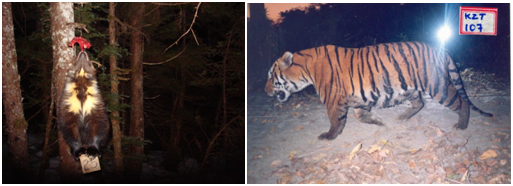
\includegraphics[width=5in]{Ch1/figs/wolverinetiger}
\end{center}
\caption{
Left: Wolverine being encounter by a
camera trap ({\it Photo credit: Audrey Magoun}).
Right: Tiger encountered by
camera trap ({\it Photo credit: Ullas Karanth/WCS}).
}
\label{fig.wolverinetiger}
\end{figure}

\subsection{DNA Sampling}

DNA obtained from hair, blood or scat is now
routinely used to obtain individual identity and encounter history
information about individuals \citep{taberlet_bouvent:1992,
  woods_etal:1999, mills_etal:2000, schwartz_monfort:2008}.  A common
method is based on the use of ``hair snares'' (Fig. \ref{fig.bearcat})
which are widely used to study bear populations
\citep{woods_etal:1999, gardner_etal:2010jwm, garshelis_etal:2006,
  kendall_etal:2009}.  A sample of hair is obtained as individuals
pass under or around barbed-wire (or other physical mechanism) to take
bait. Hair snares and scent sticks have also been used to sample felid populations
\citep{garciaalaniz_etal:2010, kery_etal:2010} and other species. Research has even shown that
DNA information can be extracted from urine deposited in the wild (e.g., in snow; see \cite{valiere_taberlet:2000})
and as a result this may prove another future data collection technique where SCR models
are useful.

\begin{figure}
\begin{center}
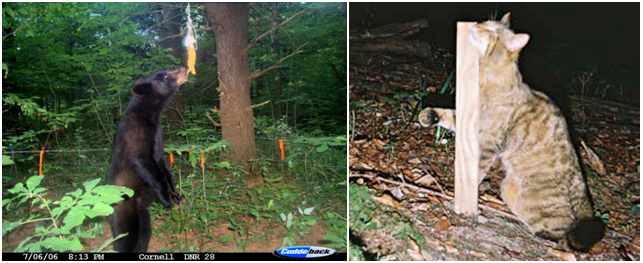
\includegraphics[width=5in]{Ch1/figs/bearcat}
\end{center}
\caption{Left:  Black bear in a hair snare ({\it Photo credit: M. Wegan})
Right: European wildcat loving on a scent stick ({\it Photo credit: Darius
Weber, Hintermann \& Weber AG, Ecological Consultancy, Planning \&
Research, Switzerland})
}
\label{fig.bearcat}
\end{figure}


\begin{figure}
\begin{center}
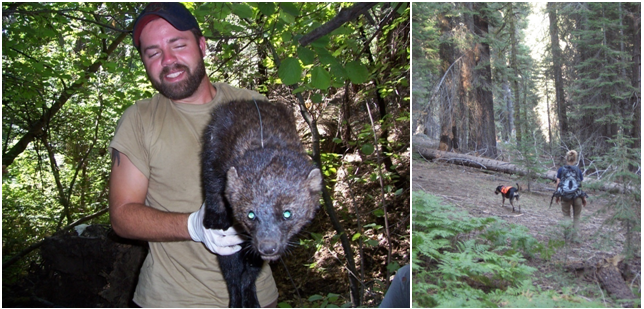
\includegraphics[width=5in]{Ch1/figs/beardog}
\end{center}
\caption{Left:
A wildlife research technician for the USDA Forest Service
  holding a male fisher  captured as part of the Kings River Fisher
  Project in the Sierra National Forest, California.
Right: A dog handler surveying for fisher scat in the Sierra National Forest.
{\it Photo credit: Craig Thompson, USDA Forest Service,
Pacific Southwest Research Station.}}
\label{fig.fisherscatdog}
\end{figure}


\subsection{Acoustic surveys}

Many studies of birds \citep{dawson_efford:2009}, bats, and whales \citep{marques_etal:2009}  now collect data using
devices that record vocalizations. When vocalizations can be identified by individual from multiple
recording devices, spatial encounter histories are produced that are amenable to
the application of SCR models \citep{dawson_efford:2009, efford_etal:2009ecol}.

\subsection{Search-Encounter Methods}

There are other methods which don't fall into a nice clean taxonomy of
``devices''. Spatial encounter histories\footnote{defined? probably
  not! need to do that} are commonly obtained by conducting manual
searches of geographic sample units such as quadrats, transects or
road or trail networks.
For example,
DNA-based encounter histories can be obtained from scat
samples located along roads or trails or by specially trained dogs
\citep{mackay_etal:2008} searching space
(Fig. \ref{fig.fisherscatdog}). This method has been used in studies
of martens, fishers \citep{thompson_etal:inpress}, lynx, coyotes,
birds \citet{kery_etal:2010}, and many other species. We might search
space on foot and pick up individuals and physically mark them
somehow. This is pretty common in surveys that involve reptiles and
amphibians, e.g., we might walk transects picking up 
box turtles \citep{hall_etal:1999}, or desert tortoises \citep{zylstra_eta:2010},
 or search space for lizards
\citep{royle_young:2008} and also surveys designed to obtain animal
scat. These methods don't seem like normal capture-recapture in the
sense that the encounter of individuals is not associated with
specific trap location, but SCR models are equally relevant for
analysis of such data (see Chapt. \ref{chapt.searchencounter}).


\section{ Historical Context: A Brief Synopsis of the Literature}

Spatial capture-recapture is a relatively new methodological
development, at least with regard to formal estimation and
inference. However, the basic problems that motivate the need for
formal spatially-explicit models have been recognized for decades and
quite a large number of ideas have been proposed to deal with these
problems. We review some of these ideas here.


\subsection{Buffering}

 The standard approach to estimating density even now is to estimate $N$ using
conventional closed population models \citep{otis_etal:1978} and then
try to associate with this estimate some specific sampled area, say $A$,
the area which is contributing individuals to the population for which
$N$ is being estimated. The strategy is to define $A$ by placing a buffer
of say $W$ around the trap array or some polygon which encloses the trap
array. The historical context is succinctly stated by \citep{obrien:2011}
from which we draw this description:

\begin{quote}
  ``At its most simplistic, $A$ may be described by a concave polygon
  defined by connecting the outermost trap locations ($A_{tp}$; \citet{mohr:1947}).
 This assumes that animals do not move from outside the
  bounded area to inside the area or vice versa. Unless the study is
  conducted on a small island or a physical barrier is erected in the
  study area to limit movement of animals, this assumption is unlikely
  to be true. More often, a boundary area of width $W$ ($A_{w}$) is added to
  the area defined by the polygon $A_{tp}$ to reflect the area beyond the
  limit of the traps that potentially is contributing animals to the
  abundance estimate \citep{otis_etal:1978}. The sampled area, also known
  as the effective area, is then $A(W) = A_{tp} + A_{w}$. Calculation of the
  buffer strip width ($W$) is critical to the estimation of density and
  is problematic because there is no agreed upon method of estimating
  $W$. Solutions to this problem all involve ad hoc methods that date
  back to early attempts to estimate abundance and home ranges based
  on trapping grids
  \citep[see][]{hayne:1949}. \citet{dice:1938} first drew attention
  to this problem in small mammal studies and recommended using
  one-half the diameter of an average home range. Other solutions have
  included use of inter-trap distances \citep{blair:1940,burt:1943}, mean
  movements among traps, maximum movements among traps \citep{holdenried:1940, hayne:1949},
 nested grids \citep{otis_etal:1978}, and assessment
  lines \citep{smith_etal:1971}.''
\end{quote}

The idea of using 1/2 mean maximum distance moved
\citep{wilson_anderson:1985a} seems to be the standard approach even
today, presumably justified by Dice's suggestion to use 1/2 the home
range diameter. Alternatively, some studies have used the full
MMDM (e.g. \citet{parmenter_etal:2003}),

%\footnote{Do they really say that?}  Yes, they really do use it, but so
%do a lot of studies so we can add more if you want.

because the trap array might not provide a full coverage of the home range so 1/2 MMDM may be smaller than the home range radius. And, sometimes home range size is
estimated by telemetry \citep{karanth:1995, bales_etal:2005}.
%\footnote{Is this correct cite for this?}.  Karanth used some technique, it's hard to tell for sure....but he
% mentions using 1 female that is collared to estimate effective trap area.  Bales does it too, so I added it for
% extra value!

This is usually combined
with an AIC-based selection from among the closed-population models in
\citet{otis_etal:1978} which most often suggests heterogeneity in detection (Model
Mh).  Almost all of these early methods were motivated by studies of
small mammals using classical ``trapping grids'' but, more recently,
their popularity has increased with the advent of new technologies and
especially related to non-invasive sampling methods such as camera
trapping. In particular, the series of papers by Karanth and Nichols
\citep{karanth:1995, karanth_nichols:1998, karanth_nichols:2002}
has led to fairly widespread adoption of these ideas.

Some of the heuristic ideas based on buffer strips do have some
technical justification in the sense of estimating parameters of an
underlying movement model from observed movements. For example, if we
let $x$ be a random variable indicating movement outcomes of an
individual about its  home range center, and suppose that $x$ has pdf
$g(x)$ then we can understand properties of MMDM by studying the
properties of the sample order statistics, as the maximum distance
moved is the sample range based on a sample of observations of
individual locations.



%As an illustration, imagine a 1-dimensional
%system where individuals have a home range that amounts to a line
%segment. Then suppose that individual movements are $\mbox{uniform}(0,A)$. It
%can be shown that the sampling distribution of the sample range, R,
%scaled by $A$, say $R/A$ has a beta distribution, $\mbox{beta}(n-1,2)$
%\citep[][p. 235]{casella_berger:2002}
%and thus the diameter of the home range, i.e. $A$, is
%estimated (biasedly) by$ R/( (n-1)/(n+1) )$. For large $n$ we could then
%say that the sample range, i.e., ''maximum distance moved'' seems like a good estimator of home range diameter and, therefore, $R/2$ is an estimator of home-range radius.

%There are a number of technical issues that arise in attempting to use
%such heuristics to justify the application in practice. For one, the
%moments of the sample order statistics are strongly affected by sample
%size, which is typically quite small (per individual encountered) and
%thus, in general, are biased and estimated with variable precision
%depending on sample size. For example, the expected value of MMDM is
%$k(n)*A$ , i.e., the true home range diameter is related to observed
%MMDM by some function of sample size, $k(n)$, that increases to 1. In
%the case where the underlying movement model is uniform, $k(n) =
%(n-1)/(n+1)$ (from above) which motivates a formula for ``adjusting''
%observed MMDM for small sample size. We suspect that many such
%formulae are obtainable depending on the assumed movement distribution
%\citep[e.g., formula 6.16 in][]{obrien:2011}. We might also think about taking
%the {\it maximum} (over individuals) of the maximum distance moved
%because under the specific model considered here (iid uniform) then
%all individuals have the same home range radius. This increases our
%sample size ($n$) and thus the observed sample range should be more
%accurate.


%%Another issue of somewhat more importance (and less easy to
%rectify) is that the {\it observation} of movement outcomes is biased
%by the locations of traps. We cannot observe movements ``off the
%trapping grid'' (or between traps) and thus our observed movements
%will generally be smaller than expected under any particular model
%(the uniform in this case). Moreover, the trap spacing also induces a
%discreteness to the movements that causes a further level of
%approximation based on hypothetical movement
%distributions. Nevertheless, formal analysis of `` buffering''
%strategies based on sample order statistics under specific models for
%movement does at least provide some heuristic support for specific
%choices.  The interested reader should ponder the distribution of the
%sample minimum, maximum and range under other distributions such as a
%normal (and bivariate normal), exponential distribution and perhaps
%others. In addition, contemplate the effect of censoring of movements
%to some arbitrary limit ($B<A$) to mimic bias in observed movement
%outcomes due to a finite trap grid.

\subsection{Trapping webs}

The use of buffer strips is conventional and widespread due to the
heuristic appeal of that idea and its easy implementation, but other
conceptual approaches exist to address specific problems motivated by
the spatial context of capture-recapture data. D.R. Anderson came up
with the idea of the ``trapping web'' \citep{anderson_etal:1983} which
does not seem to have been widely adopted in practice.
% although there
%is a clear mathematical formalization to the trapping web design
%\citep{link_barker:1994}.
One reason for this is
the design is somewhat restrictive in the sense that it requires
a large number of traps be organized in close proximity to one
another.

\subsection{Temporary Emigration}

Another intuitively appealing idea is that by \citet{white_shenk:2000}
who discuss ``correcting bias of grid trapping estimates'' by
recognizing that the basic problem is like random temporary emigration
\citep{kendall_etal:1997} where individuals flip a coin with
probability $\phi$ to determine if they are ``available'' to be
sampled or not.  White and Shenk's idea was to estimate $\phi$ from
radio telemetry, as the proportion of time an individual spends in the
study area. They obtain the estimated super-population size by using
standard closed population models and then obtain density by $\hat{D}
= \hat{N}\hat{\phi}/A$ where $A$ is the nominal area of the trapping
array (e.g., minimum convex hull).  A problem with this approach is
that individuals that were radio collared represent a biased sample
i.e., you fundamentally have to sample individuals randomly from the
population {\it in proportion to their exposure to sampling} and that
seems practically impossible to accomplish. In other words, ``in the study area'' has no
precise meaning itself and is impossible to characterize in almost all capture-recapture studies.
Deciding what is ``in the study area'' is effectively the same as choosing an arbitrary buffer which defines
who is in the study area who who isn't.
That said, the temporary
emigration analogy is a good heuristic for understanding SCR models
and has a precise technical relevance to certain models.

Another very interesting idea is that of using some summary of
``average location'' as an individual covariate in standard
capture-recapture models. \citet{boulanger_mclellan:2001} use
distance-to-edge (DTE) as a covariate in the Huggins-Alho type of
model. \citet{ivan:2012} uses this approach in conjunction with an
adjustment to the estimated $N$ obtained by estimating the proportion of
time individuals are ``on the area formally covered by the grid''
using radio telemetry.  We do not dwell too much on these different
variations but we do note that the use of DTE as an individual
covariate amounts to some kind of intermediate model between simple
closed population models and fully spatial capture-recapture models,
which we address directly in Chapt. \ref{chapt.closed}.
%We note that no adjustment
%based on telemetry information is necessary if one were simply to
%place a prior distribution on the individual covariate (which is not
%to say that telemetry data isn't useful, just that the same objective
%can be achieved without telemetry data).

While these procedures are all heuristically appealing, they are also
essentially ad hoc in the sense that the underlying model remains
unspecified or at least imprecisely characterized and so there is
little or no basis for modifying, extending or generalizing the
methods. These methods are distinctly {\it not} model-based procedures
even though they might well be heuristically appealing under specific
movement models. Despite this, there seems to be an enormous amount of
literature developing, evaluating and ``validating'' these literally
dozens of heuristic ideas that solve specific problems, as well as
various related tweeks and tunings of them and really it hasn't led to
any substantive breakthroughs that are sufficiently general or
theoretically rigorous.



%A classical argument in favor of the HA model is
%that it ``doesn't require assumptions about the covariate'' but the
%assumption is explicit in capture-recapture models and thus it is
%natural to attack inference based on the ``joint likelihood''
%\citep{borchers_etal:2002}. This has proven necessary in certain other
%classes of individual covariate models in which natural models arise
%for the individual covariate, such as time-varying individual
%covariates \citep{bonner_schwarz:2006}, or covariates with measurement
%error (e.g., distance sampling; see
%\citet[][ch. 7]{royle_dorazio:2008}).
%The model-based formulation is easily adapted to standard
%individual covariate models as well \citep{royle:2008}. Throughout
%this book we rely heavily on Bayesian inference of the joint
%likelihood, using the formulation based on data-augmentation
%\citep{royle_etal:2007, royle_young:2008, royle:2009} though we also
%discuss the development of likelihood-based inference in chapter 5 and
%apply those methods in some cases.


\section{The Failure of Classical Capture-Recapture}

XXXX Motive should probably go here , or immediately in next
section XXXXXXX


We briefly introduced and reviewed a number of classical techniques for applying non-spatial capture-recapture
models to studies of animal populations. These techniques, such as buffering, are based on many heuristically appealing
ideas.
But these are just heuristics and do not resolve the essential, basic problem with conventional
(''non-spatial'') capture-recapture models which is that there is no linkage {\it in the model} between
the quantity being informed by the data (i.e., $N$) and any stated or prescribed ``area'', $A$.

More generally,
ordinary capture-recapture methods are
distinctly non-spatial. They don't admit spatial indexing of either sampling
(the observation process) or
of individuals (the ecological process). This leads immediately to 3 main deficiencies:
 (1)
Ordinary CR models do not provide a coherent basis for estimating density.
For capture-recapture models to provide a coherent framework for inference about population density,
$N$ has to scale, as part of the model, with $A$ so that the model imposes biological context
on $A$ (i.e., as the area over which the $N$ individuals reside). SCR models achieve this.
(2) Ordinary CR models {\it induce} a form of heterogeneity that can
 only at best be approximated by classical models of latent heterogeneity. SCR models formally
 accommodate heterogeneity due to the juxtaposition of individuals with the encounter devices.
(3) Ordinary CR models do not accommodate trap-level covariates which
 exist in a large proportion of real studies. Again, SCR models formally
 accommodate heterogeneity due trap variation.  %or something like that last sentence
 %so that all 3 issues match.


Here we confront some of the issues that motivate the need for spatial
capture-recapture models by considering analysis of data from a study
design to estimate black bear abundance on the Fort Drum Military
Installation in upstate New York (see Chapt. \ref{chapt.closed} for more details). The
specific data used here are encounter histories on 47 individuals
obtained from an array of 38 baited ``hair snares'' during June and
July 2006. The study area and locations of the 38 hair snares are
shown in Fig. \ref{fig.hairsnares}.  Barbed wire traps (see
Fig. \ref{fig.bearcat}) were baited and checked for hair samples each
week for eight weeks.  Analysis of these data appears in
\citet{gardner_etal:2010jwm} and we use the data in a number of analyses
in later chapters.

\begin{figure}
\begin{center}
\includegraphics[height=3in]{Ch1/figs/hairsnares}
\end{center}
\caption{Locations of black bear hair snares on Fort Drum.}
\label{fig.hairsnares}
\end{figure}

We regarded this data set as a standard capture-recapture data set -
an encounter history matrix with 47 rows and 8 columns with entries
$y_{ik}$, where $y_{ik}=1$ if individual $i$ was captured in sample
$k$ and $y_{ik}=0$ otherwise. There is a standard closed population
model, colloquially referred to as ``model $M_0$'' (see Chapt. \ref{chapt.closed}), which
assumes that encounter probability $p$ is constant for all individuals
and sample periods.  We fitted model $M_0$ to the Fort Drum data using
traditional likelihood methods, yielding the maximum likelihood
estimate (MLE) of $\hat{N} = 49.19$ with an asymptotic standard error
(SE) of $1.9$.

The key issue in using closed population models with such data is how
on earth do we interpret this estimate of $N=49.19$ bears? Does it
represent the entire population of Fort Drum? Certainly not -- the trapping array covers less than
half of Fort Drum! (Fig. \ref{fig.hairsnares}). So to get at the total bear
population size of Fort Drum, we'd have to convert our $\hat{N}$ to
an estimate of density and extrapolate. To get at density, then,
should we
assert that $N$ applies to the southern half of Fort Drum below some
arbitrary line? Surely bears move on and off of Fort Drum without
regard to hypothetical boundaries. Without additional information
there is simply no way of converting this estimate of $N$ to density,
and hence it is really not meaningful biologically. To resolve this
problem, we will adopt the customary approach of converting $N$ to $D$
by buffering the convex hull around the trap array. The convex hull
has area $157.135$ $km^2$. We follow \citet{bales_etal:2005} in
buffering the convex hull of the trap array by the radius of the mean
female home range size.


%%%%\footnote{Did Bales et al. actually do this?}.
%HERE IS WHAT BALES DID:  First, we created a 95% minimum convex polygon
%for all radiolocations of adult females used in homerange
%analyses (Figure 1). Second,we buffered the
%100% minimum convex polygon for trapping locations
%with the approximate radius of the average
%95% minimum convex polygon home range of adult
%females (n = 13) using ArcView (ESRI, Redlands,
%Calif.).


The mean female home range radius was
estimated \citep{wegan:2008} for our study region to be $2.19$
km,
%\footnote{Is this number right out of Wegan's disseration?}
% YES, this is straight out of his thesis.
and
the area of the convex hull buffered by $2.19$ km is $277.01$
km$^2$. ({\bf R}
commands to compute the convex hull, buffer it, and compute the area
are given in the {\bf R} package \mbox{scrbook} which accompanies the
book).  Hence, the estimated density
here is approximately $0.178$ bears/km$^2$ for an estimated population
size obtained using model $M_0$.  We could assert that the problem has
been solved, go home, and have a beer.  But then, on the other hand,
maybe we should question the use of the estimated home range radius
 -- after all, this is only the female home range radius and the home ranges
 change for many reasons. Instead, we may decide to rely on a buffer width based on
one-half MMDM estimated from the actual hair snare data as is more customary
\citep{dice:1938}. In that case the buffer width is $1.19$ km, and the
resulting estimated density is increased to $0.225$ bears/ha$^2$ about
27 \% larger.  But wait - some studies actually found the full MMDM
\citep{parmenter_etal:2003} to be a more appropriate measure of
movement (e.g \citet{soisalo_cavalcanti:2006}). So maybe we should use
the full MMDM
which is $2.37$ km, pretty close to the telemetry-based estimate
and therefore providing a similar estimate of density ($0.171$
bears/ha$^2$). So in trying to decide how to buffer our trap array we
have already generated 3 density estimates. The crux of the matter is
obvious: Although it is intuitive that $N$ should scale with area --
the number of bears should go up as area increases and go down as area
decreases -- in this ad hoc approach of accounting for animal movement
$N$ remains the same, no matter what area we decide we sampled. The
number of bears and the area they live in are not formally tied
together within the model, because estimating $N$ and estimating the
area $N$ refers to are two completely independent analytical steps which are unrelated to one another by a
formal model.

Unfortunately, our problems don't end here. In thinking about the use of model $M_0$, we might naturally question
some of the basic assumptions that go into that model. The obvious one
to question is that which declares that $p$ is constant. One obvious
source of variation in $p$ is variation {\it among individuals}. We
expect that individuals may have more or less exposure to trapping due
to their location relative to traps, and so we try to model this ``heterogeneous''
encounter probability
phenomenon.
To illustrate this here are the number of traps that each individual was captured in:
\begin{verbatim}
 #traps:  1   2  3  4  5  6  9
 #bears: 23  13  6  2  1  1  1
\end{verbatim}
suggesting quite a range in traps exposed to by different bears.
%%% #bears: 19 15  5  2  2  1  1  1  1
% But, being captured in different numbers of traps is {\it not} inconsistent with a non-spatial model.
%That is if individuals roamed randomly over space with no ``home range'' then you should expect them to be captured
%in varying numbers of traps also.....
This has led many to consider
capture-recapture models that allow for individual heterogeneity in
$p$. Such models have the colloquial name of ``model $M_h$.''
We fitted this model (see Chapt. \ref{chapt.closed} for details) to the Fort Drum data
using each of the 3 buffer widths previously described (telemetry, 1/2
MMDM and MMDM), producing the estimates reported in Table
\ref{intro.tab.fdests}. While we can tell by the models' AIC that $M_h$ is
clearly favored by more than 30 units, we might still not be entirely
happy with our results. Clearly there is information in our data that
could tell us something about the exposure of individual bears to the
trap array -- where they were captured, and how many times -- but
since space has no representation in our model, we can't make use of
this information. Model Mh thus merely accounts for what we observe in
our data (some bears were more frequently captured than others) rather
than explicitly accounting for the processes that generated the data.

So what are we left with?  Our density estimates span  a range
from $0.17$ to $0.43$ bears/km$^2$ depending on which estimator of $N$ we use and
what buffer strip we apply. Should we feel strongly about one or the other?
Which buffer should we prefer?
AIC favors model $M_h$, but did it adequately account for the differences in
exposure of individuals to the trap array? Are we happy with a purely phenomenological model
for heterogeneity? One that posits that all bears are $iid$ draws from some distribution?
It assumes that all individuals are iid draws from some distribution but does not
account for the explicit mechanism of induced heterogeneity. And, further, we have information
about that (trap of capture) which model Mh ignores.
%Moreover, we could find more variations of
%model Mh to choose among, but see \citep{link:2003}.
And if we choose one type of buffer, how do we compare our density estimates
to those from other studies that may opt for a different kind of buffer?
The fact that $N$ doesn't scale with $A$, as part of the model, renders this choice
arbitrary. The buffer isn't part of the model.
\begin{comment} So
how do we characterize uncertainty of the buffer ``estimate''?  And,
in what sense is the
buffer even an estimate of something? What is it an estimate of?
\end{comment}
Clearly,
there is not a compelling solution to be derived from
this ``estimate $N$ and conjure up a buffer'' approach
and we are left not much wiser about bear density at
Fort Drum than we were before we conducted this analysis.

%%%% We could just finish this part off with a paragraph about these additional open questions -
%%%%the whipped cream of problems on the capture-recapture sundae - including the trap-level covariates;
%%%%or we could come up with some trap-level covariate example for the bears (different baits used, blabla).
\begin{comment}
Some of the open questions at this point:
How do we characterize uncertainty of the buffer ``estimate''?  And,
in what sense is the
buffer even an estimate of something? What is it an estimate of?
The summary here should be that there's not a compelling solution to be derived from
this ``estimate $N$ conjure up a buffer'' approach.
{\bf The main point that N doesn't scale with A is not made
  clearly here.}
\end{comment}


\begin{table}[ht]
\centering
\caption{Table on estimates of D for the Fort Drum data
using models $M_0$ and $M_h$ and different buffers. Model $M_h$ here
is a logit-normal mixture \citep{coull_agresti:1999}.}
\begin{tabular}{ll|cc}
\hline
model & buffer &  $\hat{D}$ & SE \\ \hline
M0   & telemetry &  0.178 & 0.178 \\
M0    & MMDM     &  0.171 & 0.171\\
M0   & 1/2 MMDM  &  0.225 & 0.225\\
Mh(ln) & telemetry &0.341 & 0.144\\
Mh(ln) & MMDM    &  0.327 & 0.138\\
Mh(ln) & 1/2 MMDM & 0.432 & 0.183\\
\end{tabular}
\label{intro.tab.fdests}
\end{table}


\section{Extension of Closed Population Models}
XXX Spatial context of populations ?? XXXXXX


The deficiency with classical closed population models is that they
have no spatial context. $N$ is just an integer parameter that applies
equally well to some population that exists in a computer, estimating the number
of unique words in a book, or a bucket full of goldfish.  The question
of {\it where} the $N$ items belong is central both to interpretation
of data and estimates from all capture-recapture studies and, in fact,
to the construction of spatial capture-recapture models considered in
this book.  Surely it must matter whether the $N$ items exist as words
in a book, or goldfish in a bowl, or birds in a forest patch! That
classical closed population models have no spatial context leads to a
number of conceptual and methodological problems or limitations as we
have discussed and even encountered in our analyses so far.

Thus, the essential problem is that classical closed population models
are too simple - they ignore the spatial attribution of traps and
encounter events, movement and variability in exposure of individuals
to trap proximity, and, because ordinary closed population models
possess no notion of ``area'',  they do not yield estimates of {\it density}.
These are not problems per se but rather just features
of an overly-simple class of models, and they should 
 be addressed formally by the development of
more general models.



\subsection{The modern age}

%Spatial capture-recapture models are
%statistical and mathematical models that extend non-spatial
%``ordinary'' capture-recapture models to accommodate the spatial
%structure inherent in sampling animal populations - i.e., trap
%locations, individual locations, and individual use of space.

The solution to the various issues that arise in the application of
ordinary capture-recapture models is to extend the closed population
model so that $N$ becomes spatially explicit.
%A natural way is to
%define a point process \citep{efford:2004} that describes how
%individuals are organized in space and that, when points are
%aggregated over space, the value $N$ is derived in a meaningful way.
%Thus, in this book, we adopt the view that the locations of the $N$
%individuals in the population are a {\it realization of a spatial
%  point process}.
\citet{efford:2004} was the first to formalize an explicit model for
spatial capture-recapture problems in the context of trapping arrays.
He adopted a Poisson point process model to describe the distribution
of individuals and then what is essentially a distance sampling
formulation of the observation model which describes the probability
of detection as a function of individual location, regarded as a
latent variable governed by the point process model. While earlier
(and contemporary) methods of estimating density from trap arrays have
been ad hoc in the sense of lacking a formal description of the
spatial model, Efford achieved a formalization of the model,
describing explicit mechanisms governing the spatial distribution of
individuals and how they are encountered by traps, but
adopted a more or less ad hoc framework for inference under that
spatial model using a simulation based method known as inverse
prediction \citep{gopalaswamy:2012}.

Recently, there has been a flurry of effort devoted to formalizing
inference under this model-based framework for the analysis of spatial
capture-recapture data \citep{royle_gardner:2011,borchers:2011,gopalaswamy:2012}.
There are two distinct lines of work which
adopt the model-based formulation in terms of the underlying point
process but differ primarily by the manner in which inference is
achieved. One approach \citep{borchers_efford:2008} is a classical inference approach based on
likelihood (see Chapt. \ref{chapt.mle}), and the other \citep{royle_young:2008} adopts a
Bayesian framework for inference (Chapts. \ref{chapt.scr0,chapt.mcmc}).

To motivate the origins and relevance of these approaches, we note
that, fundamentally, spatial capture-recapture models are related to
classical ``individual covariate'' models (colloquially referred to as
Huggins-Alho models) in capture-recapture \citep{huggins:1989,
  alho:1990}.  In particular, the individual covariate\footnote{have
  we mentioned what the individual covariate is, yet?} is observed in
these classical individual covariate models whereas it is not directly
observed in SCR models.  To accommodate that, a prior distribution for
the individual covariate is required.
%In essence then, SCR models are
%similar to a fully model-based formulation of classical Huggins-Alho
%models (see \citet{royle:2009}).
Likelihood analysis
\citep{borchers_efford:2008} proceeds by removing the random effect
from the likelihood by integration whereas Bayesian analysis
\citep{royle_young:2008} proceeds by analyzing the conditional model
directly, usually by methods of Markov chain Monte Carlo (MCMC).




\subsection{Abundance as the Aggregation of a Point Process}

Spatial point process models represent a major methodological theme in
spatial statistics \citep[][ch. xyz]{cressie:1992} and they are
widely applied as models for many ecological phenomena
\citep{stoyan_penttinen:2000,illian_etal:2008}. Point process models apply to
situations in which the random variable in question represents the
locations of events or objects: trees in a forest, weeds in a field,
bird nests, etc.  As such, it seems natural to describe the
organization of individuals in space using point process models. SCR models represent the
extension of ordinary capture-recapture models by augmenting the model with a point process
model to describe individual locations.

One
of the key features of SCR models is that the point locations are
latent, or unobserved, and we only obtain imperfect information about
the point locations by observing individuals at trap or observation
locations.  Thus, the realized locations of individuals represent a
type of ``thinned'' point process, where the thinning mechanism is not
random but, rather, biased by the observation mechanism.  It is
natural to think about the observed point process as some kind of a
compound or aggregate point process with a set of ``parent'' nodes
being the locations of individual home ranges or their centroids,
and the observed locations as
``offspring'' - i.e., a Poisson cluster process (PCP). In that
context, density estimation in SCR models is analogous to estimating the number of
parents of a Poisson cluster process \citep{chandler_royle:2012}.
% Other types of point
% process models for the realized locations have direct relevance to SCR
% models (See \citet{chandler_royle:2012}, discussed in chapter XYZ).

In the context of SCR models, we suppose there is a point on the
landscape that we'll think of as a home range center or, if this is
unappealing, we can think of it as the centroid of an individual's
activities during the time of sampling. In general, this point is
unknown for any individual but if we could track an individual over
time and take many observations then we could perhaps get a good idea
of where that point is.  We'll think of the collection of these points
as defining the spatial distribution of individuals in the
population. Most of the recent developments in modeling and inference
from spatial encounter history data, including most methods discussed
in this book, are predicated on the view that individuals are
organized in space according to a relatively simple point process
model. More specifically, we assume that the collection of individual
activity centers are ``$iid$'' random variables distributed uniformly
over some region. This is consistent with the assumption that the
activity centers represent the realization of a Poisson point process
or, if the total number of activity centers if fixed, then this is
usually referred to as a binomial point process.

%%I think we could shorten the home range paragraph; I like the definition
%%'the centroid of an individual's
%%% activities during the time of sampling'. I think the definition of
%% home range is something like the colleciton of points/sites/areas
%% an animal uses over the course of its lifetime so it's vague anyway
%% and what that definition means for the different forms of home
%%ranges - territory, migratory species etc - is pretty much left open.
We use the terms home range or activity center interchangeably. The
term ``home range center'' suggests that models are only relevant to
animals that exhibit such behavior of establishing home ranges or
territories and since not all species do that, perhaps the
construction of SCR models based on this idea is flawed. However,
 the notion of a home range center is just a conceptual
device and we don't view this concept as being strictly consistent
with classical notions of animal territories. Rather our view is
that a home range or territory is inherently dynamic, temporally, and thus it is a
transient quantity - where the animal lived during the period of
study,
a concept that is completely analogous to the
more conventional notion of utilization
distributions.
Therefore, whether or not individuals of a species establish home ranges
is irrelevant because, once a precise time period is defined, this defines a distinct region of space
that an individual must have occupied. In other
words, the definition of ``home range center'' is predicated
 on the specification of a time period over which individuals
are studied. A term that might be less offensive than ``home range
center'' is ``centroid of space usage (CSU)''
 which should not
conflict directly with preconceived understandings and interpretations
of home range.


\subsection{The state-space}

If we let ${\bf s}_{i}; i=1,2,\ldots,N$ be the locations of individual
activity centers, then the question ``what are the possible values of
${\bf s}$?'' needs to be addressed because the individual ${\bf
  s}_{i}$ are {\it unknown}. As a technical matter, we will regard
them as random effects and in order to apply standard methods of
statistical inference we need to provide a distribution for these
random effects.  In the context of the point process model, the
possible values of the point locations referred to as the
``state-space'' of the point process and this is some region or set of
points which we will denote by ${\cal S}$.
${\cal S}$ is a region within which points are located - essentially a
prior distribution for ${\bf s}_{i}$ (or, equivalently, the random effects
distribution).
%%Don't think prior has come up yet; maybe not that important here?
In animal studies as a description of
where individuals that could be captured are located it encloses our
study area -- the region within which we might have located traps or
detection devices.  The state-space of the point process should
accommodate all individuals that could have been captured in the study
area.

In the practical application of SCR models, in most cases estimates of
density will be relatively insensitive to choice of state-space
%%% I also think the rest of this paragraph could be postponed to a later chapter
unless there are meaningful features to the state-space
which should be accommodated. For example, if the region within which
traps are located contains a coastline or a huge body of water then
clipping that out of the state-space will typically have an
effect on density
(see
sec. \ref{scr0.sec.wolverine} for an illustration).
This should be expected because, insofar as the
state-space serves as a prior distribution on the latent variables
${\bf s}_{i}$ then, {\it the state-space is a
  component of the model. } We discuss choosing the state-space in
Chapt. \ref{chapt.scr0}.

When the underlying point process is well-defined, including a precise
definition of the state-space, this in turn induces a precise
definition of the parameter $N$ ``population size'' as the number of
individual activity centers located within the prescribed state-space.
A deficiency with some classical methods of ``adjustment'' is they
attempted to prescribe something like a state-space - a ``sampled
area'' - except absent any precise linkage of individuals with the
state-space. SCR models formalize the linkage between individuals and
space and, in doing so, provide an explicit definition of $N$
associated with
a well-defined spatial region, and hence
density. That is, the provide a model in which $N$ scales, as part of the model, with the
size of the prescribed state-space. In a sense, the whole idea of SCR models is that by defining
this point process and its state-space ${\cal S}$, this gives context and
meaning to $N$ which can be estimated directly for that specific
state-space. Thus, it is fixing ${\cal S}$ that resolves the problem of
``unknown area'' that we have previously discussed.
\begin{comment}
%% I find the next two sentences a little confusing
But the
existence of an explicit state-space ${\cal S}$ is kind of beside the
point -- ${\cal S}$ is really not always terribly important
itself. Instead, as soon as you give the latent variables ${\bf s}$ a
place to live, and this is recognized explicitly in the model upon which inference is based,
 then you achieve spatial explicitness of the model.
\end{comment}



\section{Elements of SCR Models}

The state-space of the latent point process is the critical element of SCR models but there
are many more aspects relevant to the formulation of SCR models for specific situations.
We address some of these in more detail in the following chapter....

Broadly speaking we differentiate
between two situations: Sampling based on fixed arrays or sampling
based on ``search encounter'' methods. The former includes things like
camera traps, hair snares, mist nets and conventional traps. Fixed
arrays limit the observation location to pre-defined points, where
traps are located. Using such methods the model is a little simpler
because the ``movement process'' of individuals is confounded with the
``observation process''.
The 2nd type of model -- search encounter models -- typically
will allow locations in continuous space, possibly only restricted by
polygon boundaries \citep{royle_young:2008}.
Search-encounter data
usually allow for the separate modeling and estimation of movement
model parameters from encounter model parameters but not always,
depending on whether replication of the sampling is done.  The
classical distance sampling model with no replication (i.e., $t=1$) is a basic model
which confounds the two processes.


Depending on the type of device being considered, certain restrictions
on the observable variable are induced which suggest specific
probability models for the observable random variable, suggesting
either binomial, Poisson or multinomial (and possibly other)
observation models.
One type of a
device is what we think of as the classical ``camera trap'' and which
\citet{efford:2011} refers to as a ``proximity detector''. We can take
pictures of or detect any number of individuals and an individual can
be caught in any number of traps, and an arbitrary number of
times. Iid Bernoulli model is convenient but if you think the
re-encounters are valuable then you can have a frequency model.  Bear
hair snares are slightly different because you cannot differentiate
re-encounters.
The standard observation model that applies for ``single-catch''
\citep{efford_etal:2004} traps posits that individuals are encountered
in at most one trap per sample occasion and traps only hold one
individual.  Unfortunately we're really screwed in the single-catch
situation.
A ``multi-catch'' is like a mist-net or other things - individual is
captured and restrained but traps hold > 1 individual. In this case,
the observation model is a multinomial. There are
many variations on all of these models and new models.







\begin{comment}

\subsection{Why is density so important? }

Knowledge of population size is a fundamental piece of information in
conservation. Since the risk of a species/population going extinct is
a function of how many individuals of that species there are, much of
conservation-related research revolves around abundance. Consider, for
example, the concept of minimum viable population size � to assess
whether a population has a good chance of persistence over some time
frame we need to know how big it is to begin with. The idea of a
minimum viable population is reflected in many applied conservation
efforts. For example, in a range-wide assessment of the jaguar�s
population status, researchers were asked to delineate Jaguar
Conservation Units (JCU�s), of which one criterion was ``holding at
least 50 jaguars'' � a number considered a substantial population
\citep{sanderson_etal:2002}.

While the importance of abundance is indisputable, there are some
major issues associated with this measure. First, you cannot compare
mere values of abundance unless they refer to a specific area. If you
look at the IUCN Red List of Endangered Species entry for the
population status of the tiger, it will tell you that there are an
estimated 1700 tigers in India but only about 20 in Cambodia
\citep{chundawat_etal:2011}. Now, this will not automatically make you
lament the state of tiger conservation in Cambodia as compared to
India (although seeing these numbers you might well lament the state
of the tiger in general), because you know these numbers refer to
countries that are extremely different in size. Rather, if you wanted
to know something about where tigers are currently doing better,
you�d probably divide the number of tigers by the countries�
areas and compare tiger densities (turns out India�s tigers are
still doing better, not by a factor of 85, as mere abundances suggest,
but by a factor of 5). Although abundance and density are obviously
directly related to each other, they are different in their
applicability. Particularly, density as a scaled measure lets us
compare results across sites (as we just demonstrated for the tiger
example). In addition, some concepts incorporated in conservation
biology explicitly deal with density. For example, population growth
rate, home ranges or the probability of epidemics/disease spread are
density-dependent; the Allee effect links individual reproductive
success to population density in low-density populations.

Second, going back to the tiger example once more, we may wonder how
researchers even came up with these numbers for total population
size. Tiger abundance can be estimated using camera-traps, because
individuals have distinct stripe patterns so that photographic data
can be analyzed with capture-recapture models. But surely, no-one ever
camera-trapped the whole of India. This is a typical situation, even
on a much smaller scale. Ecologists generally sample only a small
fraction of the area used by a species or population, but want to
estimate total population size, i.e. the number of individuals
occurring in sampled {\it and unsampled} areas. If we can use the data
from sampled area to obtain a density estimate, explicit predictions
of abundance can be made to regions of any size (assuming that density
is constant across the region we are inferring to and equal to density
in the sampled area)\footnote{Note that the way total tiger abundance
  estimates are derived for India is much more complex than just
  looking at tiger density somewhere in India and then extrapolating
  it to the entire country (for details, see \citep{jhala_etal:2011});
  we merely use these numbers here to illustrate the general
  problem.}.

To summarize, density not only influences several ecological
processes, but also allows us to compare population status among
different sites; even where total abundance is of primary interest,
density can help us arrive at a total population estimate even when
we�re unable to survey the total population. Capture-recapture
models were designed to estimate abundance, but they generally cannot
be used to formally estimate density. This limitation of non-spatial
CR models has long been recognized (REF) and several ad hoc approaches
to overcome this problem have been devised. We will discuss those and
their shortcomings in XXX. The great advantage of SCR models over
non-spatial capture-recapture models is that they formally link
abundance and area so that they actually estimate density.


\end{comment}









\section{Summary and Outlook}


Spatial capture-recapture models are an extension of ordinary
capture-recapture models to accommodate the spatial organization of
both individuals in a population and the observation mechanism (e.g.,
locations of traps).  They resolve problems which have been recognized
historically and for which various ad hoc solutions have been
suggested: heterogeneity in encounter probability due to the spatial
organization of individuals relative to traps, the need to model
trap-level effects on encounter, and that a
well-defined sample area does not exist in most studies, and thus
estimates of $N$ using ordinary capture-recapture models cannot be
related directly to density.

\subsection{The Promise of Spatial Capture-Recapture}

However, SCR models are not merely an extension of technique but
rather they represent an extention in a much more
profound way in that they make ecological processes explicit in the
model -- processes of spatial organization of individuals, movement
and space-usage of individuals. While capture-recapture models have
existed for decades this is a completely new element of
closed capture-recapture models.
This is so profoundly important because
ecological scientists study elements of ecological theory using
observational data that exhibits various biases relating to the
observation mechanisms employed. In the context of capture-recapture,
we observe individual encounter history data from which we can use SCR
models to infer where individual live, how they organize themselves in
space and move around in space and how they interact with other
individuals.  Spatial capture-recapture models show great promise in their ability
to integrate explicit ecological theories directly into the models so
that we can directly test hypotheses about either space usage (e.g.,
Chapt. \ref{chapt.ecoldist}) or movement (Chapt. \ref{chapt.searchencounter}) or the distribution of
individuals in space (Chapt. \ref{chapt.state-space}). We imagine that in the near future
SCR models will include point process models that allow for
interactions among individuals such as inhibition or  clustering (REF XXXX).

Thus, SCR models are capture-recapture models that enable ecologists
to explicitly integrate biological context and theory with encounter
history data, which is something that has always been the focus of
``open population'' models but never, until very recently, has been
considered formally in closed population models. We therefore believe
that SCR models will enable ecologists to test theories of space usage
and environmental effects, social behavior and other important
theories.


<<<<<<< HEAD
=======
\subsection{What Lies Ahead}

In the following chapters we develop a comprehensive synthesis and extension of
spatial capture-recapture models.
Roughly the first third of the book is introductory material --
In Chapt. \ref{chapt.glms} we provide the basic analysis tools to understand and
analyze SCR models - namely generalized linear models (GLMs) with random effects, and their
analysis in {\bf R} and {\bf WinBUGS}.  Because SCR models represent extensions of
basic closed population models, we cover ordinary closed population
models in Chapt. \ref{chapt.closed} wherein, along with Chapts. \ref{chapt.scr0} and \ref{chapt.poisson-mn}
\footnote{might ought to put Modeling Encounter Probability
as chapter 5 instead}, provides the basic introduction
to capture-recapture models and their spatial extension.
We will see that
SCR models are a
conceptual and technical intermediates between the class of models referred to as
model $M_h$, and so-called
individual covariate models.
We develop technical tools for likelihood (Chapt. \ref{chapt.mle})
and Bayesian analysis (Chapt. \ref{chapt.mcmc}).
The middle part of the book expands set of models that we can deal with to include alternative
observation models related to the type of encounter device (Chapt. \ref{chapt.poisson-mn}), models for encounter probability
(Chapt. \ref{chapt.covariates}), [should include search-encounter models right after Poisson-mn type models?] and provides basic tools for model fit and selection (Chapt. \ref{chapt.gof}).
[should include the design chapter right here].
Finally in the last third of the book we address more advanced stuff including modeling
space usage in the encounter process (Chapt. \ref{chapt.ecoldist}), modeling state-space covariates, covariates
that affect density, (Chapt. \ref{chapt.state-space}), open population models (Chapt. \ref{chapt.open}),
models that include unmarked individuals either entirely (Chapt. \ref{chapt.scr-unmarked})
or partially marked samples (Chapt. \ref{chapt.partialID}).

In Chapter XXXX We cover a mish-mash of ideas: using telemetry data, multiple encounter methods, alternative
point-process models, and other topics that are useful but that are not fully developed or that we don't have
room for in this book.





>>>>>>> a4f454ca316a5c34e0c913aa75c0dd27a11e84c7


\chapter{
Basic Statistical Concepts
}
\markboth{Modeling}{}
\label{chapt.modeling}


\vspace{.3in}

In the previous chapter we described basic concepts of
capture-recapture methods, and explained the limitations of
non-spatial models. We emphasized the advantages of
spatial capture-recapture methods, but we assumed very little
statistical knowledge. Although it is critical to understand the
non-technical motivation for this broad class of models, it is
impossible to fully appreciate them, and apply them to real data,
without a solid grasp of the fundamentals of statistical
inference.

In this chapter, we present a brief primer on key
statistical concepts that are referenced throughout the remainder of
this book. For some readers, this material will be familiar,
perhaps even elementary, and thus you may want to skip to the next
chapter. However, our experience is that many basic statistics courses
taken by ecologists do not emphasize the important subjects covered in
this chapter. Instead, there seems to be much attention paid to
minor details such as computing the number of degrees of freedom in
various $F$-tests, which, although useful in some contexts, do not
provide the basis for drawing conclusions from data and evaulating
scientific hypotheses---the objectives of statistical inference.

In addition to being basic, all of the material in the
beginning of this chapter is explained in numerous other
texts. %\citet{casella_burger:2002}
Excellent technical treatments that emphasize ecological
problems are given by
\citet{williams_etal:2002}, \citet{royle_dorazio:2008} and
\citet{link_barker:2010}. A very accessible introduction to some of the
topics covered in this chapter is presented in Chapter 3 of
\citet{mackenzie_etal:2006}. With all these excellent references, one
might wonder why we bother rehashing these concepts here. Our motivation is
two-fold: first, we wish to develop this material using examples
relevant to spatial capture-recapture, and second, we find that most
introductory texts are not accompanied by code that can
assist the novice. We therefore attempt to present simple \R~code
throughout this chapter so that those who struggle with equations and
mathmatical notation can learn by doing. As mentioned in the Preface,
we rely on \R~because it provides tremendous flexibility for analyzing
data and because it is free. We do not, however, try to explain how to
use \R~because there are so many good references already, inluding
\citet{venables_ripley:2002,bolker:2008,venables_etal:2012}.

Following our introduction to basic statistical concepts, we lay out our
philosophy of modeling ecological data, including spatial
capture-recapture data. We also introduce hierarchical
models, and discuss why they are relevant to so many problems in
ecology. Finally, we address the common concerns levied against the
hierarchical modeler, \emph{e.g.} assumptions are bad.

\section{Random Variables and Probability Distributions}

\subsection{Stochasticity in ecology}

Few ecological processes can be described using purely deterministic
models, and thus we need a formal method for drawing conclusions from data while
acknowledging uncertainty. This is the role of statistical inference,
which is founded on the laws of probability. For our purposes, it
suffices to be familiar with a small number of concepts from
probability theory. The most important of which is the concept of a random
variable, say $X$. We wish to know the probability that a realization
of $X$ takes on some value $x$, %. That is, we want to be able to describe
$\text{Pr}(X=x)$, or perhaps the probability that $x$ lies within some
range of valuse. An approach for acheiving such goals is to develop a
statistical model for $X$ and then estimate the parameters of the
model by fitting it to data collected during an experiment.

To clarify the concept of a random variable, let $X$ be the number of
American shad (\emph{Alosa sapidissima}) caught after $K=20$ casts at
the shad hole on Deerfield River in Massachusetts. Suppose that
we had a good day and caught $x=7$ fish. If there were no random
variation at play, we would say that the probability of catching a
fish $p$ is exactly 0.35 and we would always catch 7 shad after 20
casts. In other words, our deterministic model is $x =
0.35\times K$. In reality, however, we can be pretty sure that this
deterministic model would not be very good. Even if we knew for
certain $p \equiv 0.35$, we would expect some variation in the number
of fish caught on repeated fishing outings. To describe this
variation, we need a model that acknowledges uncertainty (i.e.,
stochasticity), and specifically we need a model that describes the
probability of catching $x$ fish given $K$ and $p$,
$\text{Pr}(X=x|K,p)$.

To specify a model for $\text{Pr}(X=x|K,p)$ we need a specific type of
function known as a probability mass function (pmf). Or, in the case
where $X$ is a continuous random variable, we need a probability density function
(pdf). We will generically refer to these as probability distributions.
Statisticians make things easier for themselves,
and more complicated for everyone else, by using different notation
for probability distributions. Sometimes you will see
$\text{Pr}(X=x|K,p)$ expressed as $f(x|K,p)$ or $f(x; K,p)$ or
$p(x|K,p)$ or $\pi(x|K,p)$ or $\mathbb{P}(x|K,p)$ or $[x|K,p]$ or even
just $[x]$! Just remember that these expressions all have the same
meaning---they are all probability distributions which tell us the
probability of observing any possible realization of the random
variable $X$.

In this book, we will use bracket notation (the last two
examples above) to represent arbitrary probability distributions. When
we wish to be specific about the probability distribution, we will do
so in one of two ways, one precise and one symbolic. Before explaining
these two options, let's choose a specific distribution as a model for
the data in our example. In this case, the natural distribution for
$[x|K,p]$ is the binomial. The precise representation of this
distribution will be shown as:
\begin{equation}
  [x|K,p] = %\text{Bin}(K,p) =
             \binom{x}{K}p^x(1-p)^{K-x}.
  \label{modeling.eq.bin}
\end{equation}
The right-hand side of this equation is the binomial pmf (described in
more detail in Sec.~\ref{sec.modeling.distributions}), and plugging in
values for the parameters $K$, and $p$ will return the probability of
observing $x$. This is precise, but cumbersome to write repetitively,
and it may make the eyes glaze over when seen too often. Thus, we will
often simplify Eq.~\ref{modeling.eq.bin} using the symbolic notation:
\begin{equation}
  x \sim \text{Bin}(K, p)
  \label{modeling.eq.binsym}
\end{equation}
%In cases where $x$ is continuous, we refer to
%$[x]$ as a probability density functions (pdf), or when
%$x$ is discrete, we call $[x]$ a probability mass functions (pmf).
%In parametric inference, we assume a particular distribution for $x$, which in
%this case would naturally be the binomial distribution, $x \sim
%\text{Binomial}(K, p)$, where $p$ is the
%probability of catching a shad on a particular cast and $K$ is the
%binomial size parameter.
The $\sim$ symbol is meant to represent a stochastic relationship, and
can be read ``is distributed as.''
%We  will use this notation to complement the bracket notation, which will
%be reserved for generic probability distributions. Thus, we could
%refer to the distribution of $x$ as
%$[x]$, with possible options being $x \sim \text{Binomial}(K,p)$ or $x \sim
%\text{Poisson}(Kp)$.
Another reason for using this notation is that
it resembles the syntax of the \bugs~language, which we will
frequently use to conduct Bayesian inference.

Now that we have specified our model as $x \sim \text{Bin}(K,p)$,
we can use it to make probability statments about future
outcomes. Continuing with our fish example, we might want to know what
the probability of catching $x=7$ again on a future fishing outing
assuming that we know $p=0.35$. Evaluating the pmf returns a
probability of 0.18, as show using this bit of \R~code:
\begin{verbatim}
> dbinom(7, 20, 0.35)
[1] 0.1844012
\end{verbatim}
By definition, the pmf allows us to evaluate the probability of observing
any $x$ given $K=20$ and $p=.35$. This probability mass distribution
can be visualized in \R~as follows:
\begin{verbatim}
plot(0:20, dbinom(0:20, 20, 0.35), type="h", ylab="Probability",
     xlab="Number of shad caught (x)")
\end{verbatim}
the result of which is shown in Fig.\ref{modeling.fig.bin} with some extra details.
\begin{figure}[ht!]
  \centering
  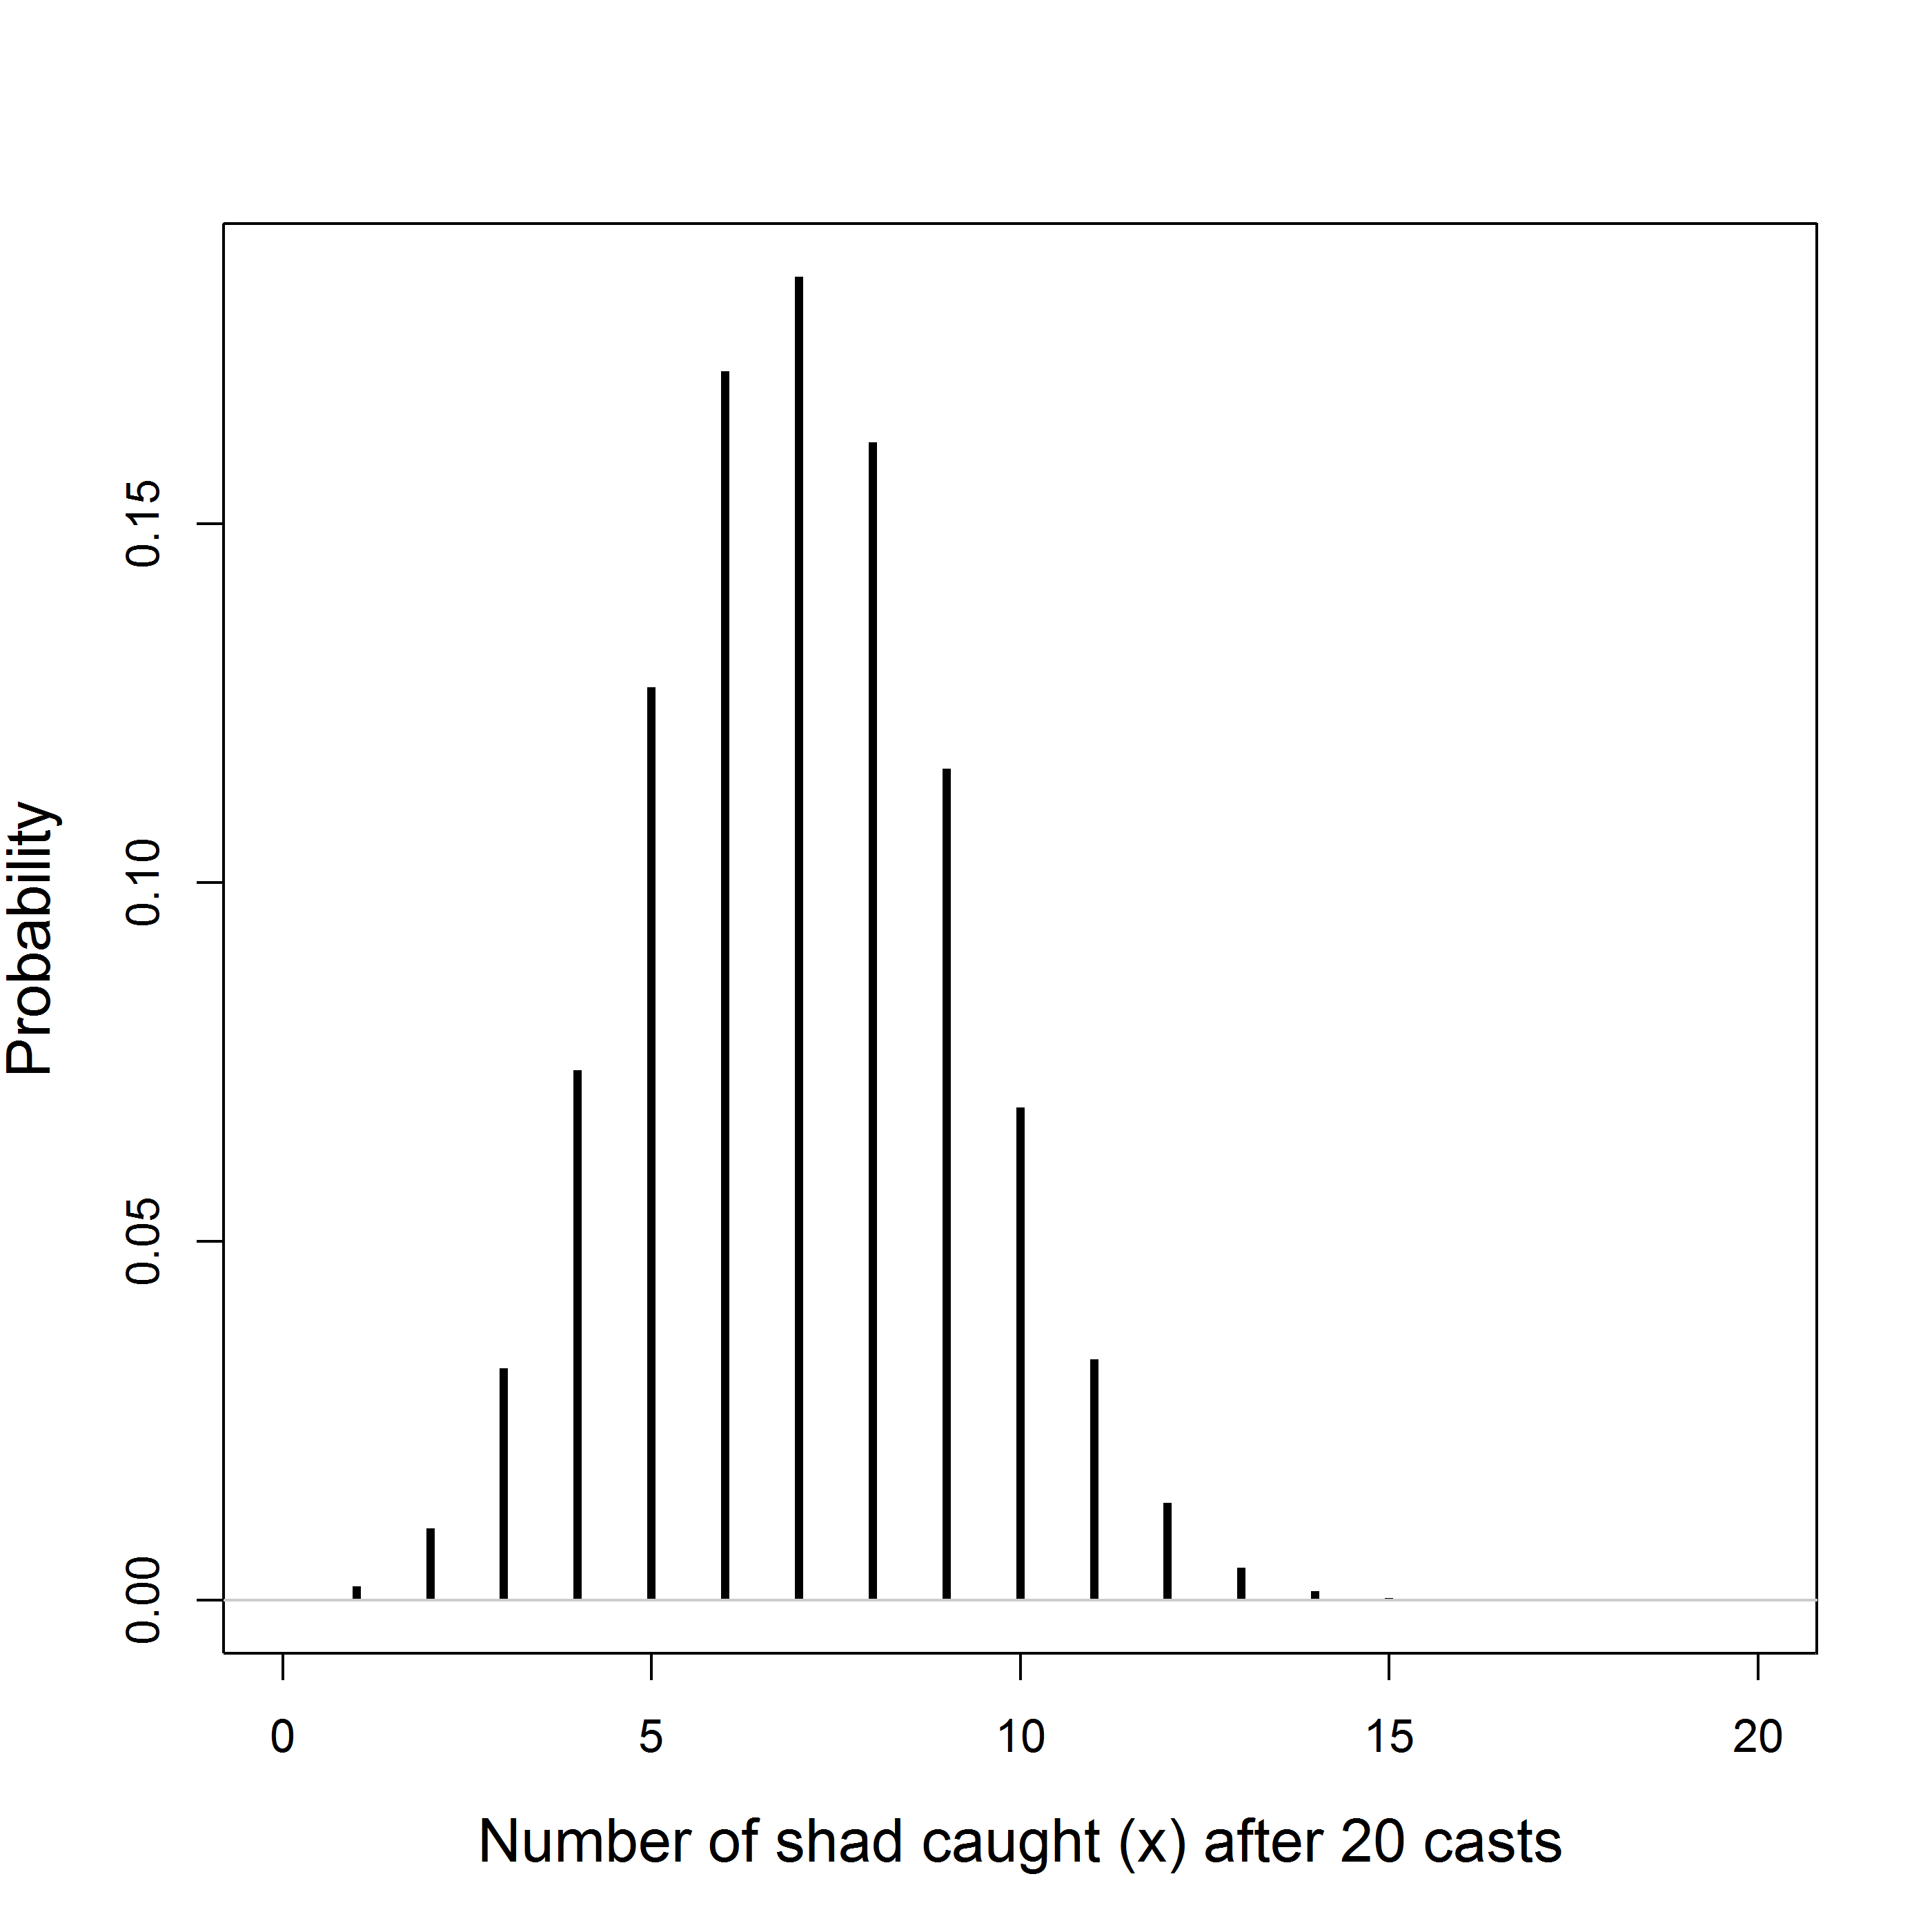
\includegraphics[width=4in,height=4in]{Ch1b/figs/bin}
\caption{The binomial probability mass function with $N=20$ and
  $p=0.35$. }
\label{modeling.fig.bin}
\end{figure}

The purpose of this little example is to show that once we specify a
model for the random variable(s) being studied, we can begin drawing
conclusions, i.e making inferences, about the processes of interest,
even in the face of uncertainty.
Probability distributions are
essential to this process, and thus we need to
understand them in some more depth.


%%%% Add support??
\begin{table}[t!]
  \small
  \caption{Common probability density functions (pdfs) and probability
    mass functions (pmfs) used throughout this book.}
  \begin{tabular}[t]{lcccc}
    \hline
    Distribution & Notation & pdf/pmf & Mean & Variance \\
    \hline
    \multicolumn{5}{c}{Discrete random variables} \\
    Poisson & $x \sim \text{Pois}(\lambda)$ &
    $\exp(-\lambda )\lambda^x/x!$ & $\lambda$ & $\lambda$ \\
    Bernoulli & $x \sim \text{Bern}(p)$ & $p^x(1-p)^{1-x}$ & $p$ &
    $p(1-p)$  \\
    Binomial & x $\sim \text{Bin}(N, p)$ & $\binom{x}{N}p^x(1-p)^{N-x}$
    & $Np$ & $Np(1-p)$  \\
    Multinomial & $\mathbf{x} \sim \text{Multinom}(N, \bm{\pi})$ &
    $\binom{N}{x_1 \cdots x_k}\pi_1^{x_1} \cdots \pi_k^{x_k}$ & $N\pi_k$
    & $N\pi_k(1-\pi_k)$ \\
    \multicolumn{5}{c}{Continuous random variables} \\
    Normal & $x \sim \text{N}(\mu, \sigma^2)$ & $\frac{1}{\sigma\sqrt{2\pi}}
      \exp(-\frac{(x-\mu)^2}{2\sigma^2})$ & $\mu$ & $\sigma^2$  \\
    Uniform & $x \sim \text{Unif}(a, b)$ & $1/(b-a)$ & $(a+b)/2$ &
    $(b-a)^2/12$  \\
%    2D-Uniform & $\mathbf{x} \sim \text{Unif}(\mathcal{S})$ & $1/A(\mathcal{S})$ & &  \\
    Beta & $x \sim \text{Beta}(a, b)$ &
    $\frac{\Gamma(a+b)}{\Gamma(a)+\Gamma(b)}x^{a-1}
    (1-x)^{b-1}$ & $a/(a+b)$ & $\frac{ab}{(a+b)^2(a+b+1)}$ \\
    Gamma & $x \sim \text{Gamma}(a,b)$ &
    $\frac{b^a}{\Gamma(a)}x^{a-1}\exp(-bx)$ & $a/b$ & $a/b^2$  \\
    \hline
  \end{tabular}
  \label{modeling.tab.pdfs}
\end{table}




\subsection{Properties of Probability Distributions}

A pdf or a pfm is a function like any other function
%Probability distributions are functions like any other functions
in the sense that it has one or more arguments whose values determine
the result(s) of the function. However, probability functions have a few
properties that distinguish them from other functions.
The first is that the function
must be non-negative for all possible values of the random variable
$X$, i.e. $[x] \geq 0$. The second requirement is that the integral of
a pdf must be unity, $\int_{-\infty}^{\infty} [x] = 1$, and similarly
for pmf, the summation over all possible values is unity, $\sum_x [x]
= 1$. The following \R~code demonstrates
this for the normal and binomial distributions:
\begin{verbatim}
> integrate(dnorm, -Inf, Inf, mean=0, sd=1)$value
[1] 1
> sum(dbinom(0:5, size=5, p=0.1)) # 5 is as good as Inf here
[1] 1
\end{verbatim}
This requirement is important to remember when one must develop a
non-standard probability distribution. For example, in Chapt.
~\ref{chapt.state-space} and \ref{chapt.rsf},
we work with a resource selection function (RSF) whose probability
density function is not one that is pre-defined in software packages
such as \R~or \bugs.

Another feature of probability distributions is that they can be used
to compute important summaries of random variables. The two most
important summaries are the expected value, $\mathbb{E}(X)$,
and the variance $\text{Var}(X)$. The expected value
can be thought of as the average
value of a very large sample from the specified distribution. For
example, a poor man's way of finding the expected values of a binomial
distribution with $K=20$ trials and $p=0.35$ can be implemented in \R~using:
\begin{verbatim}
> mean(rbinom(10000, 20, 0.3))
[1] 6.9865
\end{verbatim}
For most probability distributions used in this book, the expected
values are known exactly, as shown in Table~\ref{stat.tab.pdfs}, and
thus we don't need to resort to Monte Carlo approximations. For instance, the
expected value of the binomial distribution is $\mathbb{E}[x] = Kp =
20 \times 0.35 = 7$. In this case, it happens to take an integer
value, but this is not a necessary condition, even for discrete random
variables.

A more formal definition of an expected value is the average of all
possible values of the random variable, weighted by their
probabilities. For continuous random variables, this weighted average
is found via integration:
\begin{equation}
  \mathbb{E}(X) = \int_{-\infty}^{\infty} x[x] \, \text{d}{x}.
  \label{modeling:eq:EXc}
\end{equation}
For example, if $[x]$ is normally distributed with mean 3 and unit
variance, we could find the expected value using the following code.
\begin{verbatim}
> integrate(function(x) x*dnorm(x, 3, 1), -Inf, Inf)
3 with absolute error < 0.00033
\end{verbatim}
Of course, the mean \textit{is} the expected values for the normal
distributions, so we didn't need to compute the integral, but the
point is that Eq.~\ref{modeling:eq:EXc} is generic. For discrete
random variables, the expected value is found by summation rather than
integration:
\begin{equation}
  \mathbb{E}(X) = \sum_{x} x[x]
  \label{modeling:eq:EXd}
\end{equation}
where the summation is over all possible values of $x$.

Earlier we
approximted the expected value of the binomial distribution
with $K=20$ trials and $p=0.35$ by taking a Monte Carlo
average. Eq.~\ref{modeling:eq:EXd} let's us
find the exact answer, as done using this bit of \R~code:
\begin{verbatim}
> sum(dbinom(0:100, 20, 0.35)*0:100)
[1] 7
\end{verbatim}
This is great. But of what use is it? One very
important concept to understand is that when we fit (generalized
linear) models, we are modeling the expected value of some random
variable. For example, in Poisson regression, we model $\lambda$, the
expected value of a Poisson random variable, which may be a function
of environmental variables.

The ability to model the expected value of a random variable gets us
very far, but we also need a model for the variance of the random
variable. The variance %is itself a type of expected value; one that
describes the amount of variation around the expected
value. Specifically, $\text{Var}(X) = \mathbb{E}((X -
\mathbb{E}(X))^2)$. Clearly, if the variance is zero, the variable is
not random.

For some distributions, notably the normal distribution, the variance
is a parameter to be estimated. Thus, in ordinary linear regression,
we estimate both the mean (expected value) of the random variable
$\mu$ (which may be a function of covariates) and the variance
$\sigma^2$, or similarly the residual standard error $\sigma$. For
other distributions, the variance is not an explicit parameter to be
estiamted, and instead, the mean to variance ratio is fixed. In the
case of the Poisson distribution, the mean is equal to the
variance, $\mathbb{E}(X) = \text{Var}(X) = \lambda$. This is often viewed as a restriction because in ecology
count data often have a variance greater than the mean. However, much
of this variation can be ``explained'' by modeling the mean as a
function of covarites. Still, in cases where extra-Poisson variation
exists, other distributions such as the negative binomial or
zero-inflated Poisson distribution may be required. A similar
situation is true for the binomial distribuiton---the variance is
determined by the two parameters $K$ and $p$, $\text{Var}(X) = Kp(1-p)$. Thus
in our earlier example with $K=20$ and $p=0.35$, the variance is
4.55. Toying around with these ideas using random number generators
may be helpful. Here is some code
\begin{verbatim}
> 20*0.35*(1-0.35)             # Var(X)
[1] 4.55
> x <- rbinom(100000, 20, 0.35)
> mean((x-mean(x))^2)          # Monte Carlo approximation
[1] 4.545525
\end{verbatim}



\section{Common Probability Distributions}
\label{sec.modeling.distributions}

We got a little ahead of ourselves in the previous example by using
the binomial and Poisson distributions without fully describing them.
A solid understanding of the binomial, Poisson, multinomial, uniform,
and normal distributions is absolutely essential throughout the
remainder of the book. We will occasionally make use of other
distributions such as the beta, log-normal, multivariate-normal,
gamma, Dirichlet, etc... that can be helpful when
modeling capture-recapture data, but these distributions can be
readily understood once you are comfortable with the more commonly
used distributions described in this section.

\subsection{The Binomial Distribution}

We have already briefly introduced the binomial distribution, but we
need to describe it in more detail because of the critical role it
plays in ecology. The binomial distribution is
used for purposes as diverse as modeling count data, survival
probability, occurrence probability, and capture probability.

To describe the properties of the binomial distribution, and related
distributions, we will introduce a new example.
Suppose we are conducting a bird survey at a site in which 10
chestnut-sided warblers (\textit{Stetophaga pensylvanica}) occur and
each of these individuals has a detection probability of 0.5. The
binomial distribution is the natural choice for describing the number
of individuals that we would expect to detect in this
situation, and using our notation, we can write
$x \sim \text{Bin}(10, 0.5)$. Note that if $p \equiv 1$, the number of
individuals that we would observe on $J$ replicate surveys, $x_j$,
would not be a random variable---we would always observe
$x_j=10$. That is the observed data would exactly equal the expected
value and the variance would be zero.
\begin{comment}
  The \texttt{stats} package that comes with \R~has random number
  generators for most of the distributions we will use in this
  book. These functions always begin with \texttt{r}, as in
  \texttt{rbinom} for generating random binomial outcomes. Thus, to
\end{comment}
However, when $p<1$, we can expect that we will observe different
a different number of warblers on each replicate visit. To see this,
we can simulate data under this simple model in which $J=3$ visits are
made to the site:
\begin{verbatim}
> n <- rbinom(3, size=10, prob=0.5)
> n
[1] 6 4 8
\end{verbatim}
The vector $\mathbf{x}$ will typically differ each time you issue this
command; however, we know the probability of observing any value of
$n_j$ because it is defined by the binomial pmf. As we demonstrated
earlier, in \R~this probability can be found using the \verb+dbinom+
function. For example, the probability of observing $n_j=5$ is given by:
\begin{comment}
  Without knowing a thing about probability distributions, most people
  would recognize that the expected value of $x_j$ is $10 \times 0.5 =
  5$. That is, the most likely number of chestnut-sided warblers that
  we would expect to detect is 5. In this case, however, we did not
  observe a single 5, but rather observed counts of 6, 4, and 8
  chestnut-sided warblers on the first, second, and third surveys
  respectively. If 5 is the most likely outcome, how likely was it to
  observe these data? And what is the actual probability of observing
  a 5? These questions can all be answered by the probability mass
  function (pmf) for the binomial distribution.

  The probability of
  observing a 5 (or any other number) when $N=10$ and $p=0.5$ can be
  computed in \R~by issue the following command:
\end{comment}
\begin{verbatim}
dbinom(5, 10, 0.5)
\end{verbatim}
This simply evaluates the function shown in
Table~\ref{stat.tab.pdfs}. We could do the same more transparently, but
less efficiently, using any of the following:
\begin{verbatim}
N <- 10
n <- 5
p <- 0.5
factorial(N)/(factorial(n)*factorial(N-n))*p^n*(1-p)^(N-n)
exp(lgamma(N+1) - (lgamma(n+1) + lgamma(N-n+1)))*p^n*(1-p)^(N-n)
choose(N, n)*p^n*(1-p)^(N-n)
\end{verbatim}

Note that these three expressions differ only in how they compute the
binomial coefficient $\binom{N}{n}$, which is the number of different ways
we could observer 5 of the 10 chestnut-sided warblers at the site. The
binomial coefficient, which is read ``N choose n'' is defined as
\begin{equation}
  \label{eq:1}
  \binom{N}{n} = \frac{N!}{n!(N-n)!}
\end{equation}


\begin{comment}
Now that we know how to compute the probability of observing $n=5$ under
our model, we can compute the probability of observing any
integer $n$ and this allows us to easily visualize the
probability mass function as we did earlier.
  The following command produces a plot of the binomial pmf for
  integers 0 through 15. Notice that the probability of observing
  $n>N$ is zero.

\begin{verbatim}
plot(0:15, dbinom(0:15, 10, 0.5), type="h", lwd=5, lend="butt",
     xlab="n", ylab="Pr(n=x|N,p)")
\end{verbatim}

  In our example, we only drew 3 samples from the binomial
  distribution and it should be evident that it would be difficult to
  estimate parameters of the distribution with such a small
  sample. With a large sample, a histogram of the observed counts
  should closely mimic the true probability mass function as is shown
  here:


  This example illustrates the uncertainty inherent in sampling and
  the


  If our interest was in estimating $N$, and we somehow knew that
  $p=0.5$, our best guess would be that $N$ is the mean of the counts
  divided by the detection probability,
  \[
  \hat{N} = \frac{\mathbb{E}(x)}{p} = \frac{1/J \sum_j x_j}{p} =
  \frac{6}{0.5} = 12.
  \]
  Our estimate is 2 chestnut-sided warblers too high. Not too bad
  though. As it turns out, estimating the binomial $N$ can be quite a
  challenge, which we will discuss in more in the next section on
  estimation. For the moment, it is important to recognize what the
  binomial distribution is, and how it can be used to describe our
  hypotheses about an ecological processs. It also , however, that we
  had nothing better to do than visit the site 100 times. In this
  case, we would expect to observe counts such as this:
\end{comment}



\subsection{The Bernoulli Distribution}

Above, we showed three alternatives to \verb+dbinom+ for evaluating the
binmial pmf. These three commands differed only in how they computed
the binomial coefficient, which we needed because of the numerous ways
in which we could observe $n=5$ under our model. To conceptualize
this, let $h_i$ be the binary variable indicating if individual $i$
was detected or not.
For example, we could observed $\mathbf{h}=(0,0,1,1,1,1,1,0,0,0)$
which is to say that we detected individuals 3-7 but not 1-2 or
8-10. For $N=10$ and $n=5$, there
are 252 possiblities of $\mathbf{h}$. However, when $N \equiv 1$, this term
drops from the pmf and the result is the pmf for the Bernoulli
distribution. That is, the Bernoulli distribution is simply the
binomial distribution when $N \equiv 1$. Alternatively, we could say that the binomial
distribution is the outcome of $N$ i.i.d. Bernoulli trials.

The utility of the Bernoulli distribution is evident when we imagine
that not all of the chestnut-sided warblers have the same detection
probability. Thus, if some individuals can be detected with
probability 0.3 and others have a 0.7 detection probabilty, we can no
longer safely write $n \sim \text{Bin}(N, p)$ since $p$ is no
longer a constant (scalar). %\footnote{Although this model is not
%  technically accurate, it is often a good approximation if
%  heterogeneity in $p$ is low.}.

To properly account for variation in $p$, we could redefine our notation
describing how the counts of chestnut-sided warblers are
generated. Our model now is
\begin{gather}
h_{ij} \sim \text{Bern}(p_i) \quad \text{for} \; i=1,2,\dots,N \\
x_j = \sum_i h_{ij}
\label{modeling.eq.Bern}
\end{gather}

Note that the individual-specific data $h_{ij}$ can observed be
observed when we can keep track of each individual, such as when they
are marked or otherwise distinguishable. In such cases,
the Bernoulli distribution allows us to
model variation in detection probability among individuals and thus
would be preferable to the binomial distribution, we assumes that each
of the $N$ individuals have the same $p$.
For this reason, the Bernoulli
distribution, as simple as it is, is of paramount importance in
capture-recapture models, including spatial capture-recapture models
in which there is virtually always variation in capture probability
among individuals. Indeed, it could be said the Bernoulli model is the
canonical model in capture-recapture studies---most of the
variations in capture-recapture models lie in how $p_i$ is specified,
and how $N$ is estimated.

The Bernoulli pmf is simply $p^n(1-p)^{1-n}$ and hence we do not need canned
functions to facilitate its evaluation. Of course, if you wanted to, you
could always use \verb+dbinom+ with the \verb+size+ argument set to
1.

\subsection{The Multinomial Distribution}


Earlier we let $h_{ij}$ denote a binary variable indicating if
warbler $i$ was detected on survey $j$. The vector of observations for an
individual, $\mathbf{h}_i$, is often referred to as the individual's
``encounter history''. The number of possible encounter
histories depends on the number of survey occasssions. Specifically,
there are $2^J$
possible encounter histories\footnote{When $N$ is unknown, we can
  never observer the encounter history of an individual that is not
  detected, and thus the number of ``observable'' encounter histories
  is $2^(J-1)$}.
If we tabulate the number of individuals with each encounter history,
the frequencies can be modeled using the multinomial
distribution.

The multinomial distribution can be thought of as a
model for placing $N$ items in $K$
categories, which we will also refer to as bins or cells. Each bin has
its own probability $\pi_k$ and
these probabilities must sum to one.
In ecology, $N$ is often population size or the number of individuals
detected, but the definition of the $K$ bins varies among
applications. In standard capture-recapture models, the bins are the
capture histories and the cell probabilities are the probabilities of
observing each capture history. In
distance sampling, when the distance data are in discrete intervals,
the bins are the distance intervals, and the cell probabilities are
the probability of detection in each interval.

Going back to our
chestnut-sided warbler example, suppose the 10 individuals are marked
and we make $J=2$ visits to the site such that there are $2^J = 4$ possible encounter
histories $\mathbf{h} \in c(11, 10, 01, 00)$. If $p=1$, then the
encounter history for each of the 10 individuals would be $11$. That
is, we would detect each individual on both occasions. In this case,
we could format our data as $\mathbf{h} = (10, 0, 0, 0)$. The
cooresponding cell probabilities would be $\bm{\pi} = (1, 0, 0,
0)$. What about the situation where $p<1$, e.g. $p=0.3$? In this case, the
probability of observing the capture history ``11'' (detected on both
occasions) is $pp = 0.3 \times 0.3 = 0.09$. The probability of
observing $10$ is $p*(1-p) = 0.21$. Following this logic, the vector
of cell probabilies is $\bm{\pi} = (0.09, 0.21, 0.21, 0.49)$. We can
simulate data under this model as follows:
\begin{verbatim}
> caphist.probs <- c("11"=0.09, "10"=0.21, "01"=0.21, "00"=0.49)
> drop(rmultinom(1, 10, caphist.probs))
11 10 01 00
 0  3  2  5
\end{verbatim}\footnote{The \verb+drop+ function simply converts the matrix to a vector.}
The
result of our simulation is that zero individuals were observed with
the capture history ``11'' and 5 individuals were observed with the
capture history ``00''. The other 5 individuals were observed one out
of the two occasions. This is not such a surprising outcome given
$p=0.3$. Note that the a single outcome of a multinomial distribution
is a vector, and hence it is a multivariate distribution in contrast
to the univariate distributions discussed so far.

As in non-spatial capture-recapture studies, the multinomial
distribution turns out to be very important in spatial
capture-recapture studies. However, $N$ is typically not population
size. Rather, we use the multinomial distribution when an individual
can only be captured in a single trap during an occasion. Thus, in
this case, $N=1$ and the cell probabilities are the probabilities of
being captured in each trap.

It is worth noting that, just as the Bernoulli distribution is a specific case of the binomial
distribution when $N \equiv 1$, the categorical distribution is a very
similar to a multinomial distribution with size parameter
$N\equiv1$. The only difference is that, rather than returning a
vector with a single element equal to 1, it returns the element number
where the 1 occurs. For example, if $h=(0,0,1,0)$ is an outcome of a
multinomial distribution with $N=1$, then the categorical outcome
would be 3 because the third cell is 1. Thus, in spatial
capture-recapture models, we might use either the multinomial
distribution with $N=1$, or we can just as well use the categorical
distribution. They are equivalent.


\subsection{The Poisson Distribution}

One of the most important models for describing the distribution
of individuals in space is the Poisson point
process. If $N$ individuals are uniformly distributed in some region
$\mathcal{S}$ with area $A$, and $N$ is a
random variable, we call this the homogeneous Poisson point process
whose intensity parameter is $\lambda = 1/A$. The intensity parameter
is defined as the expected number of points that one would find in an
infinitesimally small area. Often, the intensity parameter is not
constant, but rather it takes on different values for each location
$x$ in the region $\mathcal{S}$. The inhomogeneous Poisson point
process model can be useful in such cases, and typically, the
intensity is modeled as a log-linear function of spatially-referenced
environmental covariates. Thus, rather than $\lambda$, the intensity
parameter is now $\lambda(x)$. Inhomogeneous Poisson point process
models have a long history of applications in forestry, and are now
being increasingly used to model species distributions. They are also
extremely important in spatial capture-recapture as we will soon see.

Although the Poisson point process model is very powerful when
coordinate data are available, count data are much more prevalent in
ecological studies. Here too the Poisson distribution acts as the
canonical model, and one of the reasons for this is that count data
can be thought of as spatial aggregations of point data.
Indeed, under the homogeneous Poisson point process model,
then the number of individuals occurring in some
region $B \in A$ is Poisson distributed with expectation
$\lambda = N/A$. As before, $\lambda$ might vary among regions, which
may be distinct habitat patches or arbitrarily-defined survey plots or
quadrats. Modeling spatial variation in $\lambda$ is easily done using
Poisson regression, which is a specific type of generalized linear
model.

One feature of the Poisson distribution that is easily criticized is
that it assumes the mean is equal to the variance. blah and blah.

How will we use the Poisson distribution in spatial-capture recapture
models? One of the most common applications is studies in which an
individual can be detected multiple times at a trap during a single
occasion. For example, in camera trapping studies we might obtain
multiple pictures of the same individual during a sampling
occasion. Thus, $\lambda$ in this case would be defined as the
expected number of detections per occasion.



\subsection{The Uniform Distribution}

The poor uniform distribution is perhaps the most boring of
distributions. I mean, come on, there are no parameters to estimate or
model. The only two parameters are the lower and upper endpoints,
which are almost always known. On the bright side, the uniform
distribution is one of the most widely used,
especially among Bayesians who use it to as a ``non-informative''
prior. We will do this very regularly in this book. For example, if we
have a capture probability parameter $p$ that we wish to estimate, but
we have no prior knowledge of what value it may take in the range
[0,1], we will often use the prior $p \sim \text{Unif}(0,1)$. This
simply states that $p$ is equally likely to take on any value between
zero and one.

Another common use of the uniform distribution is as a prior for the
location of points in a plane. Remember the Poisson point process
described previously---well, a simple way to simulate such data is as
follows:
\begin{verbatim}
s
\end{verbatim}
where $\mathbf{s}$ is the two-dimensional vector of
coordinates. We will often represent this model for the point
locations as
\begin{equation}
  s \sim \text{Unif}(\mathcal{S}),
\end{equation}
although, it would be more correct to somehow distiguish this
two-dimensional uniform distribution for the univariate one. That is,
it might be more clear to use notation such as
$s \sim \text{Unif}_2(\mathcal{S})$ instead. However, this is rather
tedious and cumbersome, so we will opt for the former expression.

\subsection{The Normal Distribution}

Ecologists used to model just about everything as normally
distributed. One reason for this is that methods such a linear
regression and $t$-tests were all that were available in many
primitive stats software programs. Another reason why the normal
distribution, also called the Gaussian distribution, is so attractive
is that it allows us to estimate both the mean and variance of a
random variable, and to model explicit models for each. This is really
great, but often random variables are simply not continuous and cannot
take on values between $-\infty$ and $\infty$. Think of
population size... discrete; presence-absence data... discrete;
survival times... continuous but positive, etc...


\subsection{The Beta Distribution}

Many of the parameters of interest in capture-recapture models are
probabilities---think of capture probability or survival
probability. If we think of these parameters as random variables,
as Bayesians do, then we will often describe these distributions using
the beta distribution. The beta distribution is particularly useful as
a prior for such parameters because it allows us to express either a
lack of knowledge or very precise knowledge about a
parameter. Specifically, a $\text{Beta}(1,1)$ distribution is
equivalent to a $\text{Unif}(0, 1)$ distribution. However, unlike the
the uniform distribution, the beta distribution can be used as an
informative prior; for example if published estimates of detection
probability exist.








\section{Parameter Estimation}

If we know the parameters of a model with absolute certainty, then
we can use pdfs and pmf to make direct
probability statements about unknowns such as future outcomes. However, we
almost never know the actual values of parameters, and instead we have
to estimate them. Our inferences must then acknowledge the uncertainty
associated with our imperfect knowledge of the parameters. Doing so is
most often done using one of two approaches to inference, one referred
to as classical inference and the other known as Bayesian
inference. Both types of statistical inference make heavy use of
probability distributions. In the next chapter, we will review some of
the important concepts in Bayesian inference, so here, we will
focus on classical inference.

In classical inference, if our data are distributed according to some
distribution with unknown parameter $\lambda$, then the only
uncertainty that we are concerned with is that attributable
sampling. For instance, we can imagine repeatedly sampling the
population and each time obtaining a different estimate of $\lambda$.




\section{Joint, Marginal, and Conditional Distributions}

So far we have restricted our attention to single random variables.
However, in ecology, we often are interested in multiple random
variables and how they are related. Define $Y$ as a random variable
whose realized values may or may not be independent of $X$. Inference
about these two random variables can be made using the joint,
marginal, or conditional distributions---or, we may make use of all of
them---it depends upon our question being asked. In the case of
discrete random variables, the joint
distribution is the probability that $X$ takes on the value $x$
\textit{and} that $Y$ takes on the value $y$, which is written
$[X=x,Y=y]$. To clarify this concept, let's go back to our previous
example where $X$ was the number of fish caught after 20 casts, which
we said was an independent and identically distributed (i.i.d.)
binomial random variable. Now,
let's suppose that $X$ depends on the random variable $Y$, which is
the number of other fisherman at the hole. Specifically, let's say
that the probability of catching a fish $p$ is related to $X$
according to $\text{logit}(p) = -0.6 + -2y$. Furthermore, let's
make the intuitive assumption that the number of fishermen at the hole
is a Possion random variable with mean $0.6$, i.e. $x \sim
\text{Poisson}(0.6)$. Our model is now fully specified, and so we can
answer the question, ``what is the probability of catching $x$ fish
\textit{and} of there being $y$ a-holes at the hole. This joint
distribution is given by the product of the binomial pmf (with $p$
determined by $y$), and the Poisson pmf with $\lambda=0.6$. The
following \R~code creates the joint distribution.
\begin{verbatim}
> X <- 0:20 # All possible values of X
> Y <- 0:10  # All possible values of Y
> lambda <- 0.6
> p <- plogis(-0.62 + -2*Y) # p as function of Y
> round(p,2)
 [1] 0.35 0.07 0.01 0.00 0.00 0.00 0.00 0.00 0.00 0.00 0.00
> joint <- matrix(NA, length(X), length(Y))
> rownames(joint) <- paste("X=", X, sep="")
> colnames(joint) <- paste("Y=", Y, sep="")
>
> # Joint distribution [X,Y]
> for(i in 1:length(Y)) {
+     joint[,i] <- dbinom(X, 20, p[i]) * dpois(Y[i], lambda)
+ }
> round(joint,2)
      Y=0  Y=1  Y=2  Y=3 Y=4 Y=5 Y=6 Y=7 Y=8 Y=9 Y=10
X=0  0.00 0.08 0.08 0.02   0   0   0   0   0   0    0
X=1  0.00 0.12 0.02 0.00   0   0   0   0   0   0    0
X=2  0.01 0.08 0.00 0.00   0   0   0   0   0   0    0
X=3  0.02 0.04 0.00 0.00   0   0   0   0   0   0    0
X=4  0.04 0.01 0.00 0.00   0   0   0   0   0   0    0
X=5  0.07 0.00 0.00 0.00   0   0   0   0   0   0    0
X=6  0.09 0.00 0.00 0.00   0   0   0   0   0   0    0
X=7  0.10 0.00 0.00 0.00   0   0   0   0   0   0    0
X=8  0.09 0.00 0.00 0.00   0   0   0   0   0   0    0
X=9  0.06 0.00 0.00 0.00   0   0   0   0   0   0    0
X=10 0.04 0.00 0.00 0.00   0   0   0   0   0   0    0
X=11 0.02 0.00 0.00 0.00   0   0   0   0   0   0    0
X=12 0.01 0.00 0.00 0.00   0   0   0   0   0   0    0
X=13 0.00 0.00 0.00 0.00   0   0   0   0   0   0    0
X=14 0.00 0.00 0.00 0.00   0   0   0   0   0   0    0
X=15 0.00 0.00 0.00 0.00   0   0   0   0   0   0    0
X=16 0.00 0.00 0.00 0.00   0   0   0   0   0   0    0
X=17 0.00 0.00 0.00 0.00   0   0   0   0   0   0    0
X=18 0.00 0.00 0.00 0.00   0   0   0   0   0   0    0
X=19 0.00 0.00 0.00 0.00   0   0   0   0   0   0    0
X=20 0.00 0.00 0.00 0.00   0   0   0   0   0   0    0
\end{verbatim}
This matrix tells us the probability of all possible combinations of
$x$ and $y$, and as dicatated by the law of total probability, the sum
of these probabilities is equal to 1.

Perhaps most fisherman don't care about joint distributions. But, a
question that might be asked is ``what is the probability
of catching 1 fish today?'' Well, we know that this depends upon the
number of fisherman, but we don't know how many will show up
today. This brings us to the marginal distribution, which is defined by
\begin{equation*}
  [X] = \sum_Y [X|Y] \qquad
  [Y] = \sum_X [Y|X]
\end{equation*}
for discrete random variables, and
\begin{equation*}
  [X] = \int_{-\infty}^\infty [X|Y] \, \mathrm{d}Y \qquad
  [Y] = \int_{-\infty}^\infty [Y|X] \, \mathrm{d}X
\end{equation*}
for continuous random variables. The key idea here is that to get the
marginal distribution of $X$, we have to contemplate all possible
values of $Y$. Computing marginal distributions is a key step in
maximilizing likelihoods involving random effects, as will be
demonstrated in Chapt.\ref{chapt.mle}. Here is some \R~code to compute
the marginal distribution of $X$, i.e. the probability of $X=x$ fish:
\begin{verbatim}
> margX <- rowSums(joint)
> round(margX, 2)
 X=0  X=1  X=2  X=3  X=4  X=5  X=6  X=7  X=8  X=9 X=10 X=11 X=12 X=13 X=14
0.18 0.14 0.09 0.05 0.05 0.07 0.09 0.10 0.09 0.06 0.04 0.02 0.01 0.00 0.00
X=15 X=16 X=17 X=18 X=19 X=20
0.00 0.00 0.00 0.00 0.00 0.00
\end{verbatim}
Bad news---the most likely value is $X=0$, but there is a simliar
probability of catching 1 fish.

The last type of question we can ask about these two random variables
relates to their conditional distributions. The
conditional probability distribution is the distribution of one
variable, given a realized value of the other. In the case of two discrete random
variables, the conditional distribution may be written as
$[X=x|Y=y]$, i.e. the probability of $X$ taking on the value $x$
given the realized value of $Y$ being $y$. For simplicity, we will
write this as $[X|Y]$. Conditional distributions are defined as follows:
\begin{equation*}
  [X|Y] = \frac{[X,Y]}{[Y]} \qquad [Y|X] = \frac{[X,Y]}{[X]}.
\end{equation*}
That is, the conditional distribution of $X$ given $Y$ is the joint
distbution divided by the marginal distribution of $Y$.
\begin{verbatim}
> XgivenY <- joint/matrix(margY, nrow(joint), ncol(joint), byrow=TRUE)
> round(XgivenY, 2)
      Y=0  Y=1  Y=2  Y=3 Y=4 Y=5 Y=6 Y=7 Y=8 Y=9 Y=10
X=0  0.00 0.25 0.82 0.97   1   1   1   1   1   1    1
X=1  0.00 0.36 0.16 0.03   0   0   0   0   0   0    0
X=2  0.01 0.25 0.02 0.00   0   0   0   0   0   0    0
X=3  0.03 0.11 0.00 0.00   0   0   0   0   0   0    0
X=4  0.07 0.03 0.00 0.00   0   0   0   0   0   0    0
X=5  0.13 0.01 0.00 0.00   0   0   0   0   0   0    0
X=6  0.17 0.00 0.00 0.00   0   0   0   0   0   0    0
X=7  0.18 0.00 0.00 0.00   0   0   0   0   0   0    0
X=8  0.16 0.00 0.00 0.00   0   0   0   0   0   0    0
X=9  0.12 0.00 0.00 0.00   0   0   0   0   0   0    0
X=10 0.07 0.00 0.00 0.00   0   0   0   0   0   0    0
X=11 0.03 0.00 0.00 0.00   0   0   0   0   0   0    0
X=12 0.01 0.00 0.00 0.00   0   0   0   0   0   0    0
X=13 0.00 0.00 0.00 0.00   0   0   0   0   0   0    0
X=14 0.00 0.00 0.00 0.00   0   0   0   0   0   0    0
X=15 0.00 0.00 0.00 0.00   0   0   0   0   0   0    0
X=16 0.00 0.00 0.00 0.00   0   0   0   0   0   0    0
X=17 0.00 0.00 0.00 0.00   0   0   0   0   0   0    0
X=18 0.00 0.00 0.00 0.00   0   0   0   0   0   0    0
X=19 0.00 0.00 0.00 0.00   0   0   0   0   0   0    0
X=20 0.00 0.00 0.00 0.00   0   0   0   0   0   0    0
\end{verbatim}
Note that we have 11 probability distributions for $X$, one for each
possible value of $Y$, and each pmf sums to unity as it should. Note
also that if you show up at the hole and there are more than 2
fisherman, you might want to head home (assuming you actually want to
catch a fish).
%Why is this? Well, remember that capture probability
%declined as a function of the the number of fisherman.

These concepts are explained in more detail, and with more attention
to detail, in other texts such as \citet{casella_burger:2001}, but hopefully, the
code shown here complements the equations and makes it easier for
non-statisticians to understand these concepts.

The last point we wish
to make in the section is that this simple toy example is an example
of a hierarchical model, and we can put all the pieces together using
the following notation:
\begin{gather}
  y \sim \text{Poisson}(0.6) \\
  \text{logit}(p_y) = -0.6 + -2y \\
  x|y \sim \text{Binomial}(20, p_y)
\end{gather}
From here on out, when you see such notation, you should immediately
grasp the fact that $y$ is a random variable independent of $x$, but
$x$ depends upon $y$ through $p$. Now you have the tools to make
probability statements about the random variables in this system. The
one caveat faced in reality is that we typically do not know the
values of the parameters, and instead we have to estimate them.[DETAILS]









\section{Hierarchical Models and Inference}

The term hierarchical modeling (or hierarchical model) has become
something of a buzzword over the last decade with hundreds of papers
published in ecological journals using that term.  So then, what
exactly is a hierarchical model, anyhow? Obviously, this term stems
from the root ``hierarchy'' which means:

\vspace{.1in}

{\flushleft
Definition: {\it hierarchy} (noun) -- a series of ordered groupings of people or things within a system;
}

\vspace{.1in}

In the case of a hierarchical model (hierarchical being the adjective
form of hierarchy), the ``things'' are probability distributions, and
they are ordered according to their conditional probability structure.
Thus, a hierarchical model is {\it an ordered series of models,
  ordered by their conditional probability structure}.

If we declare that the random variable $y = $ \# of times an
individual is encountered in a trap out of $K=10$ days has a
$\mbox{Bin}(10, p)$ distribution then this is but a single model and,
thus, not a hierarchical model. If, however, we declare that
\[
y \sim \mbox{Bin}(10,p)
\]
{\it and}
\[
p \sim \mbox{beta}(1,1)
\]
which is the same as the previous model but with a ``flat'' prior
distribution on $p$, then this is kind of a cheap pedestrian
hierarchical model according to our definition although it is barely
more interesting than the previous non-hierarchical model.
%% I think here in the intro you could remove this 'pedestrian hierarchical model'
%% For the readers who are not familiar (yet) with distributions and what a prior is, I think it would be mroe helpful
%% to only use the following example and explain briefly what the
%% p_{i}\sim \mbox{beta}(\mu, \tau) stands for
On the
other hand, suppose we have some meaningful group structure in this
problem such that the data arise by observing repeated Bernoulli
trials on {\it individuals}, e.g., they are eggs hatching from a
common nest (or parentage). So let $y_{i}$ be the outcomes for
individuals $i=1,2,...,N$ with
\[
y_{i} \sim \mbox{Bin}(K, p_{i})
\]
 and
\[
p_{i}\sim \mbox{beta}(\mu, \tau).
\]
Because of the meaningful group structure, this is a more interesting
hierarchical model. In fact, in the context of capture-recapture this
is a specific version of ``Model Mh'' (see Chapt. 3 and
\citet{dorazio_royle:2003}).  We should consider this a type of a
hierarchical model although we will make a further conceptual
distinction shortly that further dichotimizes the space of
hierarchical models.

A canonical hierarchical model in ecology is this
elemental model of species occurrence or distribution
\citep{mackenzie_etal:2002, tyre_etal:2003, kery:2011}:
\[
y_{i}|z_{i} \sim \mbox{Bin}(K,z_{i} \,  p)
\]
\[
z_{i} \sim \mbox{Bern}(\psi)
\]
where  $y_{i} = $ observation of presence/absence at a site $i$ and
$z_{i} = $ occurrence status ($z_{i}=1$ if a species occurs at  site
$i$ and $z_{i}=0$ if not).  This model has an important conceptual
distinction between the hierarchical model shown just previously
(Model Mh) and also other types of classical multi-level models such
as repeated measures on subjects, in that $z_{i}$ is an actual state
of nature. In that sense, $z$ is a random variable that is the outcome of a
``real'' process.   \citet{royle_dorazio:2008} used the term {\it
  explicit} hierarchical model to describe this type of model to
distinguish from hierarchical models ({\it implicit} hierarchical
models) where the latent variables don't
correspond to an actual state of nature -- but rather just soak up
variation that is unmodeled by explicit elements of the model.
At best, latent variables in such models
are a a surrogate for something of ecological relevance
(``time effects'', ``space effects'' etc.).


With these examples,
we expand on our definition of a hierarchical model as we will use it
in this book: \newline
{\flushleft {\bf Definition}: {\it Hierarchical Model}: A model with
  explicit component models that describe variation in the data due to
  (spatial/temporal) variation in {\it ecological process}, and due to
  {\it imperfect observation} of the process.
}



%\subsection{Anatomy of a hierarchical model}
%Interesting hierarchical models in ecology typically
%contain the following components:
%\begin{itemize}
%\item[{\bf 1.}] {\it Observations}, $y(s,t)$ -- ``data''
%\item[{\bf 2.}] {\it Observation model} $[y|z,\theta_1]$
%\item[{\bf 3.}] {\it State variable}, $z(s,t)$: outcome of ecological {\it process} of interest
%\item[{\bf 4.}] {\it Process model}  $[z|\theta_2]$
%\item[{\bf 5.}] {\it Parameters}, $\theta_1$, $\theta_2$, that govern
%  the observation and state processes
%\end{itemize}


\subsection{Spatial Capture-Recapture models as hierarchical models}

Most models considered in this book describe the encounter of
individuals conditional on the ``activity center'' of the individual,
which is a latent variable (i.e., unobserved random effect).  The
collection of these latent variables represents the outcome of an
ecological process describing how individuals distribute themselves
over the landscape. Moreover, how individuals are encountered in traps
is, in some cases, the result of a model governing movement.  As such,
these models are examples of hierarchical models that contain formal
model components representing both ecological process and also the
observation of that process. That is, they are explicit hierarchical
models \citep{royle_dorazio:2008} as opposed to implicit hierarchical
models.




\section{Characterization of SCR models}
\label{intro.sec.characterization}

For the purposes of this book, an SCR model is any ``individual
encounter model'' (not just ``capture-recapture''!) where auxiliary
spatial information is also obtained. To be more precise we could as
well use the term ``Spatial capture and/or recapture'' but that is
slightly unwieldy and, besides, it also abbreviates to SCR. The class
of SCR models includes traditional capture-recapture models with
auxiliary spatial information and even some
models that do not even require ``recapture'' (e.g., distance
sampling).  There is even a class of models (Chapt. \ref{chapt.scr-unmarked})
which don't require unique capture or
identification of individuals.

Conceptually SCR models involve a collection of random
variables, ${\bf s}$, ${\bf u}$ and $y$ where ${\bf s}$ are the
activity or home range centers, ${\bf u}$ is the location of the
individual at the time of sampling (i.e., where the observer records
the animal) which we think of as realizations from some movement
model, and $y$ is the ``response variable'' - what the observer
records. E.g., $y=1$ means ``detected'' and $y=0$ means ``not
detected'' but many other types of responses are possible.
A broad class of models for estimating density are unified by a
hierarchical model involving explicit models for
animal home range centers ${\bf s}$, movement outcomes ${\bf u}$, and
encounter data $y$.  In some cases, we don't observe $y$ but rather
summaries of $y$, say $n(y)$, yet it might be convenient in such cases
to retain an explicit focus on $y$ in terms of model construction.
We thus introduce a sequence of models - a hierarchical model -
to relate these random variables and it goes something like this:
{\small
\begin{verbatim}
# NEED A graphic made out of this somehow
# possibly a Directed Acyclic Graph with some parameters,
# Fixed nodes, and stochastic nodes, might look cool.

Home range center    movement model   observation model  [data summarization]
   g(s)                  h(u|s)            f(y|u)	        n(y)
\end{verbatim}
}
Thus, models covered in this book all have distinct
characteristics related to the following decomposition as a
hierarchical model:
\[
f(y|{\bf u})h({\bf u}|{\bf s})g({\bf s}).
\]

Every model we talk about in this book has either all of these
components or a subset of them. Fig.\ref{intro.fig.fig1} is an example of the whole
enchilada in which we make the following assumptions:
\begin{gather}
{\bf s}_{i} \sim \mbox{Uniform}({\cal S}) \\
{\bf u}_{ik} | {\bf s}_{i} \sim \mbox{Normal}({\bf s}_{i}, \sigma) \\
y_{ijk} | {\bf u}_{ik} \sim \mbox{Bernoulli}(p(\| x_j - u_{ik} \|)
\end{gather}
These ``assumptions'' are statistical statements of three basic hypotheses
that (1) activity centers are uniformly distributed in two-dimensional
space, (2) movements are normally distributed around the activity
centers, and (3) capture probability is a funciton of the distance
between the animal and the trap. Each of thse model components can be
modified as need to match specific hypotheses, study designs, and data
structures.

\begin{comment}

{\small
\begin{verbatim}
set.seed(36372)       # so that results can be reproduced
N <- 10               # population size
                      # create trap coordinates:
x <- cbind(rep(seq(0.1,0.9,0.2), each=5), rep(seq(0.1,0.9,0.2), times=5))
                      # generate individual home range centroids
s <- cbind(runif(N), runif(N))
                      # create nice graphic:
plot(x, pch= "+", xlim=c(0,1), ylim=c(0,1), xlab="Easting", ylab="Northing")
points(s, pch=16, col="blue")
for(t in 1:5) {
  points(cbind(rnorm(N, s[,1], 0.05), rnorm(N, s[,2], 0.05)), col="green",pch=20)
}
\end{verbatim}
}

\end{comment}

Fig. \ref{intro.fig.fig1} shows the results of executing these {\bf R} commands. The crosses
in the figure are trap locations, the blue circles are the locations
of each animal's activity center, and the green circles are animal
locations at 5 points in time.  The resulting plot not only
illustrates a simple state model for animal distribution and movement,
but it also hints at the potential influence of the distance between
animals and traps on the detection process. One would expect that the
traps in the northern part of the study area would capture more
animals than those in the south because fewer animals occur in the
south and movements are small. Clearly the encounter rate will also
depend upon the methods used to capture the animals, which we describe
in the next section.  Spatial capture-recapture models provide a
statistical formalization of these considerations.


\begin{figure}
\begin{center}
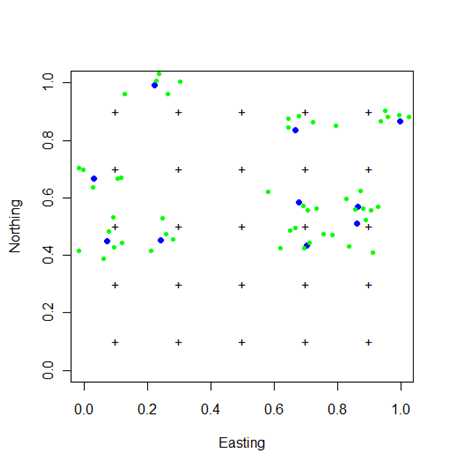
\includegraphics[height=3in]{Ch1/figs/northingeasting}
\end{center}
\caption{Population of $N$ individual home-range centers ($\bf s_i$,
  blue points) and locations during $K=5$ occasions ($\bf u_{ik}$,
  black points). Crosses represent trap locations.}
\label{intro.fig.fig1}
\end{figure}



Although the full model including $u$ and $s$ fully describes the
ecological process, in practice we usually work with reduced forms of
this model. Examples include:
of such models are:
\begin{enumerate}
\item[$\bullet$] Classical distance sampling
\item[$\bullet$] Spatial capture-recapture models with fixed arrays of traps
  \citep{efford:2004, borchers_efford:2008, royle_etal:2009ecol,
    royle_etal:2009jae, gardner_etal:2010ecol,royle_etal:2011jwm}
\item[$\bullet$] Search-encounter models \citep{royle_young:2008, royle_etal:2011mee}.
\item[$\bullet$] Capture-recapture distance-sampling \citep{borchers_etal:1998}.
\end{enumerate}
In some classes of models, components for ${\bf u}$ and ${\bf s}$ will be confounded.
e.g., if ${\bf s}$ are uniform in space and ${\bf u}$ is
a random draw from some distribution centered at ${\bf s}$, then we might as
well define ${\bf u}^{*}=\Pr({\bf u})=\int_{s} [{\bf u}|{\bf s}][{\bf
  s}]ds$ which will itself by uniform
for reasonable choices of $[{\bf u}|{\bf s}]$.  Some examples
of typical spatial capture-recapture models and how
these various model components are manifest in specific cases is
described as follows:
\begin{itemize}
\item[1.] {\bf Distance sampling -- } The last 2 stages of the hierarchy
  are confounded (implicitly) and so analysis is based on the model
  $[y|u*] [u*]$. The ``process model'' is that of ``uniformity'': ${\bf u}^{*}
  \sim Unif({\cal S})$. Sometimes it is argued that distance sampling
  estimators are ``pooling robust'' which is a way of saying they are
  (or may be)
  relatively insensitive to this assumption. That may be true, but the
  construction of distance sampling estimators makes explicit the
  uniformity assumption as a mathematical fact.

\item[2.] {\bf Spatial capture-recapture model with a fixed array of traps} --
SCR models appear to have little in common with distance sampling
because observations are made only at a pre-defined set of discrete
locations -- where traps are placed. However, the models are closely
related in terms of our hierarchical representation above\footnote{Really
they're kind of like point-count distance sampling where the identity
of individuals is preserved across point samples , and distance is a
latent variable. i.e., SCR-DS. I feel like this point should be
emphasized somehow. Here? Later?}
In SCR models based on fixed arrays,
we cannot estimate both
$\Pr(y=1|{\bf u})$ and $\Pr({\bf u}|{\bf s})$ -- the probability  that
an individual ``moves to ${\bf u}$'' cannot be seperated from the
probability that it is detected given that it moves to ${\bf u}$,
because of the fact that the observation locations are fixed by
design.
Formally, such SCR models confound $[y|{\bf u}]$  with $[{\bf
  u}|{\bf s}]$ so that the observation model arises as:
\[
 [y|{\bf s}] = \int_{u} [y|{\bf u}][{\bf u}|{\bf s}] du
\]
This confounding happens because SCR sampling is spatially biased -
restricted to a fixed pre-determined set of locations.

Conversely,
distance sampling confounds $[{\bf u}|{\bf s}][{\bf s}]$ because, essentially, there is
only a single realization of the encounter process.

It is probably
reasonable to assume that $\Pr(y=1|{\bf u})=1$ or at least it is locally
constant for most devices (e.g., cameras, etc..), and thus the
detection model will have the interpretation in terms of movement (see
chapter XXX.YY).

\item[3.] {\bf Search-encounter models -- } What we call
  ``search-encounter'' models \citep{royle_etal:2011mee}
  are kind of a hybrid model - combining features of SCR models and
  features of distance sampling. Like distance sampling they allow for
  encounters in continuous space which provide direct observations
  from $[{\bf u}|{\bf s}]$.
Thus, the
  hierarchical model is fully identified.

\item[4.] {\bf Capture-recapture/distance-sampling -- } See
  \citet{borchers_etal:1998}. As with the search-encounter models the
full hierarchical model is identified:
$[y|{\bf u}][{\bf u}|{\bf s}][{\bf s}]$ but the quantities don't
really mean the same thing as before.

To understand this, we expand the model to accommodate imperfect
measurements of ${\bf u}$. Let ${\bf u}_{obs}$ be an observation of
${\bf u}$ (i.e., made with error). A larger hiearchical model is this:
\[
[y|{\bf u}][{\bf u}_{obs}|{\bf u}][{\bf u}|{\bf s}][{\bf s}]
\]
If we make replicate ``instantaneous'' observations of location, then
information is provided about
 $[{\bf u}_{obs}|{\bf u}]$ (i.e., measurement error). However, in a normal
 distance sampling application, with instantaneous sampling, we don't
 learn anything about $[{\bf u}|{\bf s}]$,
in effect, we are again confounding $[{\bf u}|{\bf s}]$ and $[{\bf
  s}]$: ${\bf u}^{*} = \int_{s} [{\bf u}|{\bf s}][{\bf s}] ds$. So the CR-DS model focuses on:
\[
[y|{\bf u}^{*}][{\bf u}_{obs}|{\bf u}^{*}][{\bf u}^{*}].
\]
Structurally, this is the same basic model as the search-encounter
model notwithstanding (1) that it is usually talked about in terms of
repeated measures of distance instead of location and (2) the 2nd
component of the hierarchy is not movement (an ecological process) but
rather ``measurement error'' and (3) the third component is not a home
range center but rather a movement outcome (``instantaneous
location'').  Thus, while the models are structurally identically, the
meaning and interpretation of quantities are distinct.

%These are
%mostly all semantic and conceptual distinctions which are easy to
%define in a convenient table:
%\begin{table}[ht]
%\centering
%\title{What things mean in each model.}
%\begin{tabular}{c|cc}
%           &   Search encounter models     &  CR-DS  \\  \hline
%  $\sigma$    &  movement       &   measurement error  \\
% ${\bf s}$ & activity center & instaneous location \\
%\end{tabular}
%\end{table}
\end{itemize}

Efford's characterization:
proximity detectors, multi-catch, single-catch, etc....
acoustic detectors, ....

\section{Analysis of spatial capture-recapture models}





%\begin{comment}
\subsection{Models don't have political views!}

Whereas hierarchical modeling is a conceptual and framework for
formulating models, the method of inference is independent of model
formulation. Hierarchical models can be analyzed by Bayesian and
non-Bayesian methods. A model is not Bayesian or frequentist -- what
you do to that model is Bayesian or frequentist!
\[
\bullet \mbox{"Hierarchical model"} \ne  \mbox{"Bayesian"}!!!
\]
Thus, analysis of hierarchical models is easily achieved using either
Bayesian or classical (likelihood, frequentist) methods. By
``analysis'' we mean any type of estimation, characterization of
uncertainty, prediction, model selection, or evaluation and we are not
dogmatic about our choice of inference methods. That said, we do
recognize a benefit of the Bayesian approach which is that it
emphasizes model construction and not the construction of
procedures. The Nobel prize\footnote{called something else besides
  Nobel, officially} winning econometrician Christopher Sims (Slides
from the Hotelling Lecture 6/29/2007 at Duke University - cite his
webpage) said it this way: ``Bayesian inference is a way of thinking,
not a basket of 'Methods''' Conversely, ecologistis that are subjected
to a classical statistical curriculum often have only a vague sense of
what the model is that any particular procedure is employing.  We
agree with Little \citet{little:2006}
that there should be more emphasis on understanding statistical
modeling, and less emphasis on statistical methods.  Toss the ``basket
of methods'' out the window and learn how to model!

%\end{comment}

We rely strictly on principles and procedures of {\it parametric
  inference} in our analysis of hierarchical models in general and,
specifically, of spatial capture-recapture models. Parametric
inference is that in which we make explicit probability assumptions
about how the data were generated. Inference procedures are then
developed under the assumption that the model is truth, because formal
parametric inference procedures that we understand the joint
probability distribution of everything that is a realization of a
random variable. {\bf There is something missing in the previous sentence. require, maybe?}There are two popular flavors of parametric
inference: {\bf Classical inference}: The joint probability distribution
of observations is the {\bf likelihood}. We maximize it to obtain MLEs
and do other fun things to it. We evaluate procedures by thinking
about what would happen over replicate realizations of data to which
our procedures are applied.  {\bf Bayesian inference} is based on the
posterior distribution, which is the joint probability distribution of
the data and also parameters and possibly other quantities including
latent variables or random effects.

Because SCR models contain a collection of latent variables - random
effects -- a natural framework for classical analysis of the models is
based on integrated likelihood \citep{laird_ware:1982,berger_etal:1999}. That is, while
the observation model is conceptualized conditional on the random
effects (the locations of individuals), classical inference is
formally based on the likelihood constructed from the {\it marginal}
probability distribution of the observations (i.e., {\it
  unconditional} on the random effect). The random effects are removed
from the conditional likelihood by integration (which is accomplished
numerically in spatial capture-recapture models). This approach to
inference has been formalized in the context of SCR models by
\citet{borchers_efford:2008, efford:2011}, and implemented for some
classes of models in the software package {\bf DENSITY} \citep{efford:2004}
and the {\bf R} package \mbox{\tt secr} \citep{efford:2011}.

Bayesian analysis is another natural framework for the analysis of
models containing latent variables or random effects.  Under this
approach, analysis of the model is based on Monte Carlo simulation
from the posterior distribution, which is the product of the
conditional likelihood, the distribution of the random effects, and
perhaps other distributions.  This approach was developed by
\citet{royle_young:2008}, and was motivated by work focused on
modeling individual effects in capture-recapture models. In
particular, a convenient reparameterization of individual covariate
models can be obtained using a method known as data augmentation
\citep{royle_etal:2007}, see \citet{royle:2008} for an application to
classical individual covariate models in \citet{royle:2008}. The close
similarity between individual covariate models and spatial
capture-recapture models, with the individual's activity center ${\bf
  s}$ being the individual covariate, led to the application of the
data augmentation method described by \citet{royle_young:2008} and subsequent papers.

These two technical formulations (classical inference based on
integrated likelihood and Bayesian inference) both provide rigorous solutions to
the inference problems posed by spatial capture-recapture data.  There
are also minor distinctions to be aware of. For example,
as a technical matter, \citet{borchers_efford:2008} and related work, assume
a Poisson point process that is unconditional on $N$ whereas Royle and
Young (2008) and related work assume a binomial point process model
which is conditional on $N$.
%More importantly, Borchers and Efford
%develop the analysis in a way that is unconditional on the point
%process (which is removed from the conditional likelihood by
%integration).  Conversely, the analysis of \citet{royle_young:2008} is
%conditional on the underlying point process. As a technical matter,
%Bayesian analysis allows us to analyze the model that is conditional
%on the underlying point process and will otherwise have more
%flexibility - open populations, using telemetry data, etc.. as will be
%demonstrated in later chapters.

We tend to favor Bayesian inference for conceptual and philosphical
reasons but we also think that  integrated likelihood
for complex point process models may prove difficult. On the other
hand, we suspect that Bayesian
analysis by MCMC
of the model that is conditional on the underlying point process will
prove to be more versatile and generalizable for complex point process
models. We say this only
tentatively and throughout this book we are not exclusive in our views
of inference and use Bayesian and classical methods of inference
interchangeable and opportunistically in this book.
We don't want to get too much into the technical foundations of
Bayesian analysis because there are many good books now including
\citet{link_barker:2010}.  \citet{kery:2010, mccarthy:2007,
  king_etal:2009} and probably others by the time this book is
finished. That said,  Bayesian analysis is introduced at a
level required to get through this book in Chapter 2.


%\subsection{Implementing hierarchical models}



\subsection{Estimation}


Maximum likelihood: point estimates, var-covar matrix, confidence
intervals

Bayesian: analytical, simulation (MCMC)




\subsection{Modeling covariate effects}

identity, log, logit, cloglog links


Dummy variables





\section{Criticisms of Hierarchical Models}

\hl{If we keep this, remove all SCR references b/c Andy will address
  those in Chapt 5}

We have frequently used the terms
``assumptions'' and ``priors'', which make some people feel
uneasy. Our view is that expressed eloquently by Link (ADD
QUOTE). Furthermore, we note that hierarchical models allow us to
modify any assumption deemed too
restrictive. That is, we can always generalize our models given enough
data. Chapter is a classic example because it addresses
perhaps the most common criticism of SCR, that ``real animals'' don't
have symmetic home ranges. In fact people have written entire papers
beating up on SCR because they \emph{assume} that this the bivariate
normal model for the encounter processes is a rigid requirement of SCR
methods. Although we believe this assumption is quite reasonable in
many contexts, Chapter \ref{chapt.ecoldist} clearly illustrates that
alternatives exist, and that SCR provides a rigours framework for
testing for departures from this assumption, and even evaluating
hypotheses that may explain why animals move the way they do.




\chapter{
Bayesian Analysis of GL(M)Ms Using R/WinBUGS
}
\markboth{Bayesian Analysis of GLMMS}{}
\label{chapt.glms}

\vspace{.3in}

%%%% STUFF TO DO
%%% 1. Prior lack of invariance to transformation stuff: Reference and Figure
%%% 4. reference for sampling from f() with bounded support
%%% 6. Check Bayesian p-value definition
%%% 8. spell check this document

%%% NEW STUFF TO DO
%%% Add followind data/functions to REPO: R code for mcmc for Poisson regression, bugs model for BBS data
% XXX Should DIC/selection/FIT material go into Chapter 8? XXXXXXX

%%% I think the footnote on one versus several chains is too much here; maybe move to MCMC chapter?
%%% some ref chapters need filling in; eg section 3.8; section 3.8.2
%%% Once Ch2 is ready, ask Richard to go over the sections on Poisson and Binommial GL(M)Ms to make sure there isn't too much redundancy between Ch2 and 3

A major theme of this book is that spatial capture-recapture models
are, for the most part, just generalized linear models (GLMs) wherein
the covariate, distance between trap and home range center, is
partially or fully unobserved  -- and therefore regarded as
a random effect. Such models
are usually referred to as Generalized Linear Mixed Models (GLMMs)
and, therefore, SCR models can be thought of as a specialized type of
GLMM. Naturally then, we should consider analysis of these slightly
simpler models in order to gain some experience and, hopefully,
develop a better understanding of spatial capture-recapture models.

In this chapter, we consider classes of GLM models - Poisson and
binomial (i.e., logistic regression) GLMs - that will prove to be
enormously useful in the analysis of capture-recapture models of all
kinds. Many readers are likely familiar with these models because
they represent probably
the most generally useful models in all of Ecology and, as
such, have received considerable attention in many introductory and
advanced texts. We focus on them here in order to introduce the
readers to the analysis of such models in {\bf R} and {\bf WinBUGS},
which we will
translate directly to the analysis of SCR models in subsequent
chapters.

Bayesian analysis is convenient for analyzing GLMMs because it allows
us to work directly with the conditional model -- i.e., the model that
is conditional on the random effects, using computational methods
known as Markov chain Monte Carlo (MCMC). Learning how to do Bayesian
analysis of GLMs and GLMMs in {\bf WinBUGS} is, in part, the purpose
of this chapter.  While we use {\bf WinBUGS} to do the Bayesian
computations, we organize and summarize our data and execute {\bf
  WinBUGS} from within {\bf R} using the useful package \mbox{\tt
  R2WinBUGS} \citep{sturtz_etal:2005}.  \citet{kery:2010}, and
\citet{kery_schaub:2011} provide excellent introductions to the basics
of Bayesian analysis and GLMs within {\bf WinBUGS} at an accessible level. 
We don't want to
be too redundant with those books and so we avoid a detailed
treatment of Bayesian methodology - instead just providing a cursory
overview so that we can move on and attack the problems we're most
interested in related to spatial capture-recapture.  In addition,
there are a number of texts that provide general introductions to
Bayesian analysis, MCMC, and their applications in Ecology including
\citet{mccarthy:2007}, \citet{kery:2010}, \citet{link_barker:2009}, and
\citet{king_etal:2009}.


While this chapter is about Bayesian analysis of GLMMs, such models
are routinely analyzed using likelihood methods too, as discussed by
\citet{royle_dorazio:2008} and \citet{kery:2010}. 
Indeed, likelihood
analysis of such models is the primary focus of many applied
statistics texts, some good ones being \citet{mccullagh_nelder:1989} and \citet{zuur_etal:2009}. Later in
this book, we will use likelihood methods to analyze SCR models but,
for now, we concentrate on providing a basic introduction to Bayesian
analysis because that is the approach we will use in a majority of
cases in later chapters.

%Richard will move this section to previous chapter
\section{ Notation}

We will sometimes use conventional ``bracket notation'' \index{bracket
  notation} to refer to
probability distributions. If $y$ is a random variable then $[y]$
indicates its distribution or its probability density/mass function
(pdf, pmf) depending on context. If $x$ is another random variable
then $[y|x]$ is the conditional distribution of $y$ given $x$, and
$[y,x]$ is the joint distribution of $y$ and $x$. To differentiate
specific distributions in some contexts we might label them $g(y)$,
$g(y|\theta)$, $f(x)$, or similar. We will also write $y \sim
\mbox{Normal}(\mu,\sigma^{2})$ to indicate that $y$ ``is distributed as'' a normal
random variable with parameters $\mu$ and $\sigma^{2}$. The expected value
or mean of a random variable is $E[y] = \mu$ ,and $Var[y] = \sigma^{2}$ is
the variance of $y$.   To indicate specific observations we'll use an
index such as ``$i$''. So, $y_{i}$ for $i=1,2,\ldots,n$ indicates
observations for $n$ individuals. Finally, we write $\Pr(y)$ to indicate specific probabilities, i.e., of events ``$y$'' or similar.


To illustrate these concepts and notation, suppose $z$ is a binary
outcome (e.g., species occurrence) and we might assume the model: $z
\sim \mbox{Bern}(p)$ for observations.  Under this model $\Pr(z=1) =
\psi$, which is also the expected value $E[z] = \psi$. The variance is
$Var[z] = \psi*(1-\psi)$ and the probability mass function (pmf) is $[z]
= \psi^{z} (1-\psi)^{1-z}$. Sometimes we write $[z|\psi]$ when it is
important to emphasize the conditional dependence of $z$ on $\psi$. As
another example, suppose $y$ is a random variable denoting whether or
not a species is detected if an occupied site is surveyed. In this
case it might be natural to express the pmf of the observations $y$
{\it conditional} on $z$. That is, $[y|z]$. In this case, $[y|z=1]$ is
the conditional pmf of $y$ given that a site is occupied, and it is
natural to assume that $[y|z=1] = \mbox{Bern}(p)$ where $p$ is the
``detection probability'' - the probability that we detect the
species, given that it is present. The model for the observations $y$
is completely specified once we describe the other conditional pmf
$[y|z=0]$. For this conditional distribution it is sometimes
reasonable to assume $\Pr(y=1|z=0) = 0$ (\citet{mackenzie_etal:2002};
see also \citet{royle_link:2006}). That is, if the species is absent,
the probability of detection is 0. This implies that
$\Pr(y=0|z=0)=1$. To allow for situations in which the true state $z$
is unobserved, we  assume that $[z]$ is Bernoulli with parameter
$\psi$.  In this case, the marginal distribution of $y$ is
\[
 [y] = [y|z=1]Pr(z=1) + [y|z=0]Pr(z=0)
\]
because $[y|z=0]$ is a point mass at $y=0$, by assumption, the marginal
probability that $y=1$ is
\[
\Pr(y=1) = p \psi
\]
and the marginal probability that $y=0$ is
\[
\Pr(y=0) = (1-p)*\psi + (1-\psi)
\]
%END of section Richard will move to previous chapter

\section{
GLMs and GLMMs}
\label{glms.sec.glmms}
We have asserted already that SCR models work out most of the time to
be variations of GLMs and GLMMs. Some of you might therefore ask: What
are GLMs and GLMMs, anyhow?   These models are covered extensively in
many very good applied statistics books and we refer the reader
elsewhere for a detailed introduction.  The
classical reference for GLMs is \citet{nelder_wedderburn:1972} and
also \citet{mccullagh_nelder:1989}. In addition, we think \citet{kery:2010},
\citet{kery_schaub:2011}, and \citet{zuur_etal:2009} are all
accessible treatments of considerable merit. 
Here, we'll give the 1
minute
treatment of GLMMs, not trying to be complete but rather only
to preserve a coherent organization to the book.


The generalized linear model (GLM) is an extension of standard linear
models by allowing the response
variable to have some distribution from the exponential family of
distributions (i.e., not just normal). This includes the normal
distribution but also dozens of others such as the Poisson, binomial,
gamma, exponential, and many more. In addition, GLMS allow the
response variable to be related to the predictor variables (i.e.,
covariates) using a link function, which is usually nonlinear.  
%Finally, GLMs typically
% accommodate a relationship between the mean and variance.
% The GLM consists of three components:
% \begin{itemize}
% \item[1.] A probability distribution for the dependent variable $y$,
% from the exponential family of probability distributions.
%\item[2.] A ``linear predictor'' $\eta = {\bf x}'{\bm \beta}$  .
% \item[2.] A ``linear predictor'' $\eta = \beta_0 + x \beta_1$, where $x$ is the predictor variable.
% \item[3.] A link function $g$ that relates $E[y]$ to the linear predictor, $E[y] = \mu = g^{-1}(\eta)$. Therefore $g(E[y]) = \eta$.
% \end{itemize}
% XXXX ISNT THIS REDUNDANT? XXXXXXXXX
% The dependent variable $y$ is assumed to be an outcome from a
% distribution of the exponential family. The mean of the distribution of $y$ is assumed to depend on predictor variables $x$ according to
% \[
%  %g(E[y]) = {\bf x}'{\bm \beta}
%  g(E[y]) =\beta_0 + x \beta_1
% \]
% where $E[y]$ is the expected value of $y$, and ${\bf x}'{\bm \beta}$
% is termed the {\it linear predictor}, i.e., a linear function of the
% predictor variables ${\bf x}$ with unknown parameters ${\bm \beta}$ to be
% estimated.  
% The function $g$ is the link function. In standard GLMs,
% the variance of $y$ is a function $V$ of the mean of $y$: $Var(y) =
% V(\mu)$ (see below for examples).
% XXXXXXXXXXXXXXXXXXXXXXXXXXXXXXXXXXXXX SEEMS REDUNDANT UP TO HERE XXXXXXXXXXXXXXXX

The GLM consists of three components:
\begin{itemize}
\item[1.] A probability distribution for the dependent variable $y$,
from the exponential family of probability distributions.
\item[2.] A ``linear predictor'' $\eta = \beta_0 + x \beta_1$, where $x$ is the predictor variable.
\item[3.] A link function $g$ that relates the expected value of $y$, $E[y]$, to the linear predictor, $E[y] = \mu = g^{-1}(\eta)$. Therefore $g(E[y]) = \eta = \beta_0 + x \beta_1$ .
\end{itemize}

So $g(E[y])$ is assumed to be a linear function of the
predictor variable(s), here $x$, with unknown parameters, here $\beta_0$ and $\beta_1$, to be
estimated. In standard GLMs,
the variance of $y$ is a function $V$ of the mean of $y$: $Var(y) =
V(\mu)$ (see below for examples).

As an example, a Poisson GLM posits that $y \sim \mbox{Poisson}(\lambda)$ with $E[y]
=\lambda$ and usually the model for the mean is specified using the
{\it log link function} by
\[
{\text log}(\lambda_{i}) = \beta_0 + \beta_{1} \times x_{i}
\]
The variance function is $\mbox{V}(y_{i}) = \lambda_{i}$.  

To vizualize how a (Poisson) GLM works, use the {\bf R} code below.
\begin{verbatim}
set.seed(13)
n=100 #set sample size
beta0<--2 # set intercept term
beta1<- 1.5 #set coefficient
x<-rnorm(n, 0,1) #generate a predictor variable, x
linpred<-beta0+beta1*x # calculate the linear predictor of E[y]
y<-rpois(n, exp(linpred), 1) # generate observations, y, from above model
\end{verbatim} 

Using the {\tt glm()} command fits a GLM to the data we just generated and returns estimates of $\beta_0$ and $\beta_1$, which are fairly close to the data generating values above:
\begin{verbatim}
glm(y~1+x, family='poisson') #fit model

Call:  glm(formula = y ~ 1 + x, family = "poisson")

Coefficients:
(Intercept)            x  
     -2.007        1.446  

[... some output deleted ...]
\end{verbatim}

The
binomial GLM posits that $y_{i} \sim \mbox{Binomial}(K,p)$ where $K$
is the fixed sample size parameter and $E[y_{i}] = K*p_{i}$. Usually
the model for the mean is specified using the {\it logit link
  function} according to
\[
 \text {logit}(p_{i}) = \beta_{0} + \beta_{1} \times x_{i}
\]
Where $\text {logit}(u) = \text {log}(u/(1-u))$.  The inverse-logit function,
consequently, is $\text {logit}^{-1}(u) =
\text {exp}(u)/(1+\text {exp}(u))$.

A GLMM is the extension of GLMs to accommodate ``random
effects''. Often this involves adding a normal random effect to the
linear predictor, and so a simple example is:
\[
 \log(\lambda_{i}) = \alpha_{i} + \beta_{1}*x_{i}
\]
where
\[
 \alpha_{i} \sim \mbox{Normal}(\mu,\sigma^{2})
\]
%Many other probability distributions and formulations of the linear
%predictor might be considered.  It is not widely appreicated that
%the link function and
%distribution of the random effect interact directly to affect the
%implied probability distribution of the linear predictor. For the
%Poisson case just considered, $\lambda_{i}$ has a log-normal
%distribution. However, if we set $\lambda_{i} = \alpha_{i}exp(\beta*x_{i})$
%where $\alpha_{i}$ has a Gamma distribution, then $\lambda_{i}$ has
%similarly a gamma distribution with modified scale parameter.  These
%different model assumptions are seldom evaluated formally in practice
%although in many practical situations (in ecology), they imply
%specific things about the ecological process being studied
%(e.g., see \citet{royle_dorazio:2008} section XYZ on occupancy
%logit/cloglog etc..).



\section{Bayesian Analysis}

Bayesian analysis is unfamiliar to many ecological researchers because
older cohorts of ecologists were largely educated in the classical
statistical paradigm of frequentist inference. But advances in
technology and increasing exposure to benefits of Bayesian analysis
are fast making Bayesians out of people or at least making Bayesian
analysis an acceptable, general alternative to classical, frequentist
inference.

Conceptually, the main thing about Bayesian inference is that it uses
probability directly to characterize uncertainty about things we don't
know.  ``Things'', in this case, are parameters of models and, just as
it is natural to characterize uncertain outcomes of stochastic
processes using probability, it seems natural also to characterize
information about unknown ``parameters'' using probability. At least
this seems natural to us and, we think, most ecologists either
explicitly adopt that view or tend to fall into that point of view
naturally.  Conversely, frequentists use probability in many different
ways, but never to characterize uncertainty about
parameters\footnote{To hear this will be shocking to some readers
  perhaps.} Instead, frequentists use probability to characterize the
behavior of {\it procedures} such as estimators or confidence
intervals (see below). It is surprising that people readily
adopt a philosophy of statistical inference in which the things you
don't know (i.e., parameters) should {\it not} be regarded as random
variables, so that, as a consequence, one cannot use probability to
characterize ones state of knowledge about them.


\subsection{Bayes' Rule}

As its name suggests, Bayesian analysis makes use of Bayes' rule in
order to make direct probability statements about model
parameters. Given two random variables $z$ and $y$, Bayes' rule relates
the two conditional probability distributions $[z|y]$ and $[y|z]$ by
the relationship:
\[
[z|y] = [y|z][z]/[y]
\]
Bayes' rule itself is a mathematical fact and there is no debate in
the statistical community as to its validity and relevance to many
problems. Generally speaking, these distributions are characterized as
follows: $[y|z]$ is the conditional probability distribution of $y$
{\it given} $z$, $[z]$ is the marginal distribution of $z$ and $[y]$
is the marginal distribution of $y$. In the context of Bayesian
inference we usually associate specific meanings in which $[y|z]$ is
thought of as ``the likelihood'', $[z]$ as the ``prior'' and so on. We
leave this for later because here the focus is on this expression of
Bayes' rule as a basic fact of probability.

As an example of a simple application of Bayes' rule,
consider the problem of determining species presence at a sample
location based on imperfect survey information. Let $z$ be a binary
random variable that denotes species presence $(z=1)$ or absence
$(z=0)$, let $\Pr(z=1) = \psi$ where $\psi$ is usually called
occurrence probability, ``occupancy'' \citep{mackenzie_etal:2002} or ``prevalence''.
Let $y$ be the {\it observed} presence
($y=1$) or absence ($y=0$) (or detection and non-detection, to be 100 \% correct), and let $p$ be the probability that a
species is detected in a single survey at a site given that it is
present. Thus, $\Pr(y=1|z=1)=p$. The interpretation of this is that,
if the species is present, we will only observe it with
probability $p$. In addition, we assume here that $\Pr(y=1|z=0) =
0$. That is, the species cannot be detected if it is not present which
is a conventional view adopted in most biological sampling problems (but
see \citet{royle_link:2006}).
If we survey a site $T$ times but never detect the species,
then this clearly does not imply that the species is not present
($z=0$) at this site (we could just fail to observe it every single time). Rather, our degree of belief in $z=0$ should be
made with a probabilistic statement,
$\Pr(z=1|y_1=0,\ldots,y_{T}=0)$. If the $T$ surveys are independent so
that we might regard $y_{t}$ as $iid$ Bernoulli trials, then the total
number of detections, say $y$, is Binomial with probability $p$, and
we can use Bayes' rule to compute the probability that the species is present
given that it is not detected in $T$ samples. In words, the expression
we seek is:
\[
\Pr(\mbox{present} | \mbox{not detected}) = \frac{\Pr(\mbox{not detected} |
  \mbox{present})\Pr(\mbox{present})}{\Pr(\mbox{detected})}
\]
Mathematically, this is
\begin{eqnarray*}
\Pr(z=1|y=0) &= &\frac{\Pr(y=0|z=1)\Pr(z=1)}{\Pr(y=0) } \\
             &= & \frac{(1-p)^{T} \psi}{ (1-p)^T \psi + (1-\psi) }.
\end{eqnarray*}
To apply this,
suppose that $T=2$ surveys are done at a wetland for a species of
frog, and the species is not detected there. Suppose further that $\psi
= .8$ and $p = .5$ are obtained from a prior study.  Then the
probability that the species is present at this site is
$(1-0.5)^2 \times.8/((1-0.5)^2 \times 0.8 + (1-0.8) = 0.5$. 
That is, there seems to be about a
50/50 chance that the site is occupied despite the fact that the
species wasn't observed there.

In summary, Bayes' rule provides a simple linkage between the
conditional probabilities $[y|z]$ and $[z|y]$, which is useful whenever
one needs to deduce one from the other.

\subsection{Bayesian Inference}

Bayes' rule as a basic fact of probability is not disputed.
What is controversial to some is the scope and manner in which Bayes'
rule is applied by Bayesian analysts. Bayesian analysts assert that
Bayes' rule is relevant, in general, to all statistical problems by
regarding all unknown quantities of a model as realizations of random
variables - this includes data, latent variables, and also
parameters. Classical (non-Bayesian) analysts sometimes object to
regarding parameters as outcomes of random variables. Classically,
parameters are thought of as ``fixed but unknown'' (using the
terminology of classical statistics). Of course, in Bayesian analysis
they are also unknown and, in fact, there is a single data-generating
value and so they are also fixed. The difference is that this fixed
but unknown value is regarded as having been generated from some
probability distribution. Specification of that probability
distribution is necessary to carryout Bayesian analysis, but it is not
required in classical frequentist inference.


To see the general relevance of Bayes' rule in the context of
statistical inference, let $y$ denote observations - i.e., data -
and let $[y|\theta]$ be the observation model (often colloquially
referred to as the ``likelihood'').  Suppose $\theta$ 
is a parameter of
interest having (prior) probability distribution $[\theta]$. These are
combined to obtain the posterior distribution using Bayes' rule, which
is:
\[
 [\theta|y]= [y|\theta][\theta]/[y]
\]
Asserting the general relevance of Bayes' rule to all statistical
problems, we can conclude that the two main features of Bayesian
inference are that: (1) parameters, $\theta$, are regarded as realizations of
a random variable and, as a result, (2) inference is based on the
probability distribution of the parameters given the data,
$[\theta|y]$,
which is
called the posterior distribution. This is the result of using Bayes'
rule to combine the ``likelihood'' and the prior distribution.  The
key concept is regarding parameters as realizations of a random
variable because, once you admit this conceptual view, this leads
directly to the posterior distribution, a very natural quantity upon
which to base inference about things we don't know -  including
parameters of statistical models.  In particular, $[\theta|y]$ is a
probability distribution for $\theta$ and therefore we can make direct
probability statements to characterize uncertainty about
$\theta$.

The denominator of our invocation of Bayes' rule, $[y]$,
is the marginal distribution of the data $y$.  We note without further
remark right now that, in many practical problems, this can be an
enormous pain to compute. The main reason that the Bayesian paradigm
has become so popular in the last 20 years or so is because methods
have been developed
for characterizing the posterior distribution that do not
require that we possess a mathematical understanding of $[y]$. This means,
we never have to compute it or know what it looks like, or know
anything specific about it.

A common misunderstanding on the distinction between Bayesian and
frequentist inference goes something like this ``in frequentist
inference parameters are fixed but unknown but in a Bayesian analysis
parameters are random.'' At best this is a sad caricature of the
distinction and at worst it is downright wrong. A Bayesian
assumes, just like a frequentist, that there was a single
data-generating value of that parameter - a fixed, and unknown value
that produced the given data set.
The distinction between Bayesian and frequentist approaches is that
Bayesians regard the parameter as a random variable, and its value as
the outcome of a random variable, on par with the observations. This
allows Bayesians to use probability to make direct probability
statements about parameters. Frequentist inference procedures do not
permit direct probability statements to be made about parameter
values -- because parameters are not random variables!

While we can understand the conceptual basis of Bayesian inference
merely by understanding Bayes' rule -- that's really all there is to it
-- it is not so easy to understand the basis of classical
frequentist inference. 
% which is mostly like
% \footnote{as characterized by Christopher A. Sims, winner of the 
% Sveriges Riksbank Prize in Economic Sciences in Memory of Alfred Nobel
% in his
% Hotelling Lecture 6/29/2007 at Duke University - 
% \url{http://sims.princeton.edu/yftp/EmetSoc607/AppliedBayes.pdf}:
% ``Bayesian inference is a way of thinking,
% not a basket of 'Methods'''} a ``basket of
% methods'' with little coherent organization. 
What is mostly coherent
in frequentist inference is the manner in which items are evaluated -- the performance of a given procedure is
evaluated by ``averaging over'' hypothetical realizations of $y$,
regarding the {\it estimator} as a random variable. For example, if
$\hat{\theta}$ is an estimator of $\theta$ then the frequentist is
interested in $E_{y}[\hat{\theta}|y]$ which is used to characterize
bias. If the expected value of $\hat{\theta}$, when averaged over
realizations of $y$, is equal to $\theta$, then $\hat{\theta}$ is
unbiased.

The view of parameters as fixed constants and estimators as random variables
leads to interpretations that are not so straightforward. For
example confidence intervals having the interpretation ``95\%
probability that the interval contains the true value" and p-values
being "the probability of observing an outcome as extreme or more than
the one observed.'' These are far from intuitive interpretations to
most people.  Moreover, this is conceptually problematic to some
because the hypothetical realizations that characterize the
performance of our procedure we will never get to observe.

While we do tend to favor Bayesian inference for the conceptual
simplicity (parameters are random, posterior inference), we mostly
advocate for a pragamatic non-partisian approach to inference because,
frankly, some of the frequentist methods are actually very
convenient in certain situations as we will see in later chapters.


\subsection{Prior distributions}
%add paper richard mentioned in the meeting...

The prior distribution $[\theta]$ is an important feature of Bayesian
inference. As a conceptual matter,
the prior distribution characterizes ``prior beliefs'' or ``prior
information'' about a parameter. Indeed,
an oft-touted benefit of Bayesian analysis is the ease with which
prior information can be included in an analysis. 
However, more commonly, the prior is chosen to
express a lack of prior information, even if previous studies have
been done and even if the investigator does in fact know quite a bit
about a parameter.
This is because
the manner in which prior information is embodied in a prior (and the
amount of information) is
usually very subjective and thus the result can wind up being very
contentious, e.g., different investigators might report different
results based on subjective assessments of prior information. Thus it is usually
better to ``let the data speak'' and use priors that reflect absence
of information beyond the data set being analyzed. An example for an uninformative prior is a Uniform(0,1) for a probability, or a Uniform(-$\infty$, $\infty$) (also called a ``flat'' or ``improper'' prior) for an unbounded continuous parameter. Alternatively, people use ``diffuse prior''; these contain some information, but (ideally) not enough to actually influence the posterior. An example for a diffuse prior could be a Normal distribution with a large standard deviation.

But still the need occasionally arises to embody prior information or
beliefs about a parameter formally into the estimation scheme.
 In SCR models we often have a parameter that is closely linked
to ``home range radius'' and thus auxiliary information on the home
range size of a species can be used as prior information, which may improve parameter estimation (e.g., see
\citet{chandler_royle:2012} ; also Chapt. \ref{chapt.scr-unmarked}).

Other times the situation arises where a prior can inadvertently impose
substantial information on a parameter and that is not desireable.
For example, we use data augmentation
to deal with the fact that $N$ is an unknown parameter
 \citep{royle_etal:2007} which is equivalent to imposing a $Binomial(M,\psi)$
 prior on $N$ for some integer $M$. One has to take care to make sure
 that $M$ is sufficiently large so as to not affect the posterior
 distribution on $N$ (see Fig. \ref{mcmc.fig.timeseries2}).
Another situation that we have
 to be careful of is that
prior 
distributions are {\it not} invariant to transformation of the
parameter,
and therefore neither are posterior distributions
\citep[][sec. 6.2.1]{link_barker:2010}. Thus, a prior that is ostensibly
noninformative on one scale, may be very informative on another
scale. 
For example, if we have a flat prior on $\mbox{logit}(p)$ for some probability
parameter $p$, this is very different from having a 
\mbox{Unif}(0,1) prior 
on $p$. We show an example where this makes a difference in Chapt. \ref{chapt.scr0}.

\subsection{Posterior Inference}

In Bayesian inference, we are not focusing on estimating a single
point or interval but rather on characterizing a whole distribution --
the posterior distribution -- from which one can report any summary of
interest. A point estimate might be the posterior mean, median, mode,
etc..  In many applications in this book, we will compute 95\%
Bayesian confidence intervals using the 2.5\% and 97.5\% quantiles of the
posterior distribution. For such intervals, it is correct to say
$\Pr(L < \theta < U) = 0.95$. That is, "the probability that $\theta$
is between $L$ and $U$ is $0.95$". 

As an
example, suppose we conducted a Bayesian analysis to estimate
detection probability ($p$) of some species at a study site, and we
obtained a posterior distribution of beta(20,10) for the parameter
$p$. The following {\bf R} commands demonstrate how we make inferences based
upon summaries of the posterior distribution. Fig. \ref{densityvsdetection.fig} shows the
posterior along with the summary statistics.

\begin{verbatim}
> (post.median <- qbeta(0.5, 20, 10))
[1] 0.6704151
> (post.95ci <- qbeta(c(0.025, 0.975), 20, 10))
[1] 0.4916766 0.8206164
\end{verbatim}

Thus, we can state that there is a 95\% probability that $\theta$ lies
between 0.49 and 0.82.

\begin{figure}
\begin{center}
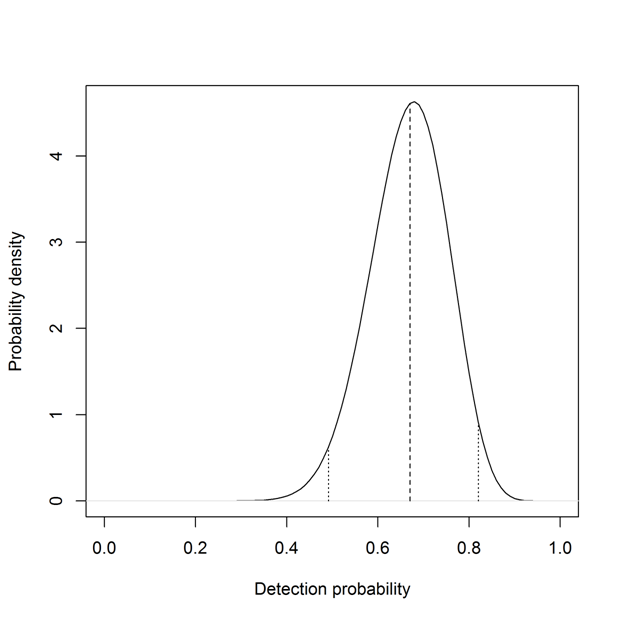
\includegraphics[height=2.5in]{Ch2/figs/densityvsdetection}
%get figure file from Ch7 folder
\end{center}
\caption{Probability density plot of a hypothetical
 posterior distribution of beta(20,10); dashed lines 
 indicate mean and upper and lower 95\% interval}
\label{densityvsdetection.fig}
\end{figure}

It is not a subtle thing that this
cannot be said using frequentist methods - although people tend to say
it anyway and not really understand why it is wrong or even that it is
wrong. This is actually a failing of frequentist ideas and the
inability of frequentists to get people to overcome their natural
tendency to use probability - which is something that, as a
frequentist, you simply cannot do in the manner that you would like
to.


% As a conceptual matter, Bayesian inference based on the posterior
% allows us 
%  to make an inference conditional on the data that we
% actually observed, i.e., what we actually know.  To us, this seems
% logical - to condition on what we know. Conversely, frequentist
% inference is based on considering average performance over
% hypothetical unobserved data sets (i.e., the ``relative frequency''
% interpretation of probability).  Frequentists know that their
% procedures work well when averaged over all hypothetical, unobserved,
% data sets but no one ever really knows how well they work for the
% specific data set analyzed. That seems like a relevant question to
% biologists who oftentimes only have their one, extremely valuable,
% data set. 
\begin{comment}
 This distinction comes into play a lot in exposing
philosophical biases in the peer review of statistical analyses in
ecology in the sense that, despite these opposing conceptual views to
inference (i.e., conditional on the data you have, or averaged over
hypothetical realizations), those who conduct a Bayesian analysis are
often (in ecology, almost always) required to provide a frequentist
evaluation of their Bayesian procedure.
\end{comment}


\subsection{Small sample inference}

The posterior
distribution is an exhaustive summary of the state-of-knowledge
about an unknown quantity. It is the posterior distribution - not an
estimate of that thing. It is also not, usually, an approximation
except to within Monte Carlo error (in cases where we use simulation
to calculate it, see Sect. \ref{glms.sec.convergence}).  One of the great virtues of Bayesian analysis which
is not really appreciated is that it is completely valid for any
particular sample size. i.e., it is $[\theta|y]$, as precise as we
claim it to be based on our ability to do calculations, for the
particular sample size and observations that we have even if we have
only a single datum $y$.  The same cannot be said for almost all
frequentist procedures in which estimates or variances are very often
(almost always in practice) based on ``asymptotic approximations'' to
the procedure which is actually being employed.

There seems to be a prevailing view in statistical ecology that
classical likelihood-based procedures are virtuous because of the
availability of simple formulas and procedures for carrying out
inference, such as calculating standard errors, doing model selection
by AIC, and assessing goodness-of-fit.  In large samples, this may be
an important practical benefit, but the theoretical validity of these
procedures cannot be asserted in most situations involving small
samples.  This is not a minor issue because it is typical in many
wildlife sampling problems - especially in surveys of carnivores or
rare/endangered species - to wind up with a small, sometimes extremely
small, data set, that is nevertheless extremely valuable \citep{foster_harmsen:2012}. For example, a recent paper on the fossa
(\emph{Cryptoprocta ferox}), an endangered carnivore in Madagascar, estimated
an adult density of 0.18 adults / km sq based on 20 animals captured
over 3 years \citep{hawkins_racey:2005}. A similar paper on the
endangered southern river otter (\emph{Lontra provocax}) estimated a density
of 0.25 animals per river km based on 12 individuals captured over 3
years \citep{sepulveda_etal:2007}. \citet{gardner_etal:2010ecol} analyzed
data from a study of the Pampas cat (\emph {Leopardus colocolo}), a species for which very little
is known, wherein only 22 individual cats were captured during the
two year period.  \citet{trolle_kery:2005} reported only 9 individual
ocelots captured and \citet{jackson_etal:2006} captured 6 individual
snow leopards (\emph{Panthera uncia}) using camera trapping. Thus, almost all likelihood-based
analysis of data on rare and/or
secretive carnivores necessarily and flagrantly violate one of Le
Cam's Basic Principles, that of ``If you need to use asymptotic
arguments, do not forget to let your number of observations tend to
infinity.''\citep{lecam:1990}.

The biologist thus faces a dilemma with such data. On one hand, these
datasets, and the resulting inference, are often criticized as being
poor and unreliable. Or, even worse\footnote{Actual quote from a
  referee}, ``the data set is so small, this is a poor analysis.''  On
the other hand, such data may be all that is available for species
that are extraordinarily important for conservation and management.
The Bayesian framework for inference provides a valid, rigorous, and
flexible framework that is theoretically justifiable in arbitrary
sample sizes. This is not to say that one will obtain precise
estimates of density or other parameters, just that your inference is
coherent and justifiable from a conceptual and technical statistical
point of view. That is, ffor example when we estimate the density $D$ of some animal population, we report the posterior probability
$\Pr(D|data)$ which is easily interpretable and just what it is
advertised to be and we don't need to do a simulation study to
evaluate how well some approximate $\Pr(D|data)$ deviates from the
actual $\Pr(D|data)$ because they are precisely the same quantity.

\begin{comment}
% note this is a distinction between SCR and CR not Bayes and non-BAyes
SCR better than ordinary CR 
for analysis of all
CR data sets because they more efficiently use the available information 
that is inherent in almost all capture-recapture studies.
\end{comment}


\section{Characterizing posterior distributions by MCMC simulation}

In practice, it is not really feasible to ever compute the marginal
probability distribution $\Pr(y)$, the denominator resulting from
application of Bayes' rule. For decades this impeded the adoption of
Bayesian methods by practitioners. Or, the few Bayesian analyses done
were based on asymptotic normal approximations to the posterior
distribution. While this was useful stuff from a theoretical and
technical standpoint and, practically, it allowed people to make the
probability statements that they naturally would like to make, it was
kind of a bad joke around the Bayesian water-cooler to, on one hand,
criticize classical statistics for being, essentially, completely ad
hoc in their approach to things but then, on the other hand, have to
devise various approximations to what they were trying to
characterize. The advent of Markov chain Monte Carlo (MCMC) methods
has made it easier to calculate posterior distributions for just about
any problem to arbitrary levels of precision.

Broadly speaking, MCMC is a class of methods for drawing random
samples
(i.e., simulating from or just ``sampling'') from the target posterior
distribution.  Thus, even though we might not recognize the posterior
as a named distribution or be able to analyze its features
analytically, e.g., devise mathematical expressions for the mean and
variance, we can use these MCMC methods to obtain a large sample from
the posterior and then use that sample to characterize features of the
posterior. What we do with the sample depends on our intentions --
typically we obtain the mean or median for use as a point estimate,
and take a confidence interval based on Monte Carlo estimates of the
quantiles. 
\begin{comment}
% tried to make point here about difference between approximations
% but failed
 These are estimates, but not like frequentist
estimates. Rather, they are Monte Carlo estimates with an associated
Monte Carlo error which is largely determined arbitrarily by the
analyst. They are not estimates qualified by a sampling distribution
as in classical statistics. If we run our MCMC long enough then our
reported value of $E[\theta|y]$ or any feature of the posterior
distribution is precisely what we say it is. There is no ``sampling
variation'' in the frequentist sense of the word.  In summary, the
MCMC samples provide a Monte Carlo characterization of {\it the}
posterior distribution.
\end{comment}


\section{What Goes on Under the MCMC Hood}

We will develop and apply MCMC methods in some detail for spatial
capture-recapture models in Chapt. \ref{chapt.mcmc}. Here we provide
a simple illustration of some basic ideas related to the practice of MCMC.

A type of MCMC method relevant to most problems is Gibbs sampling 
\citep{geman_geman:1984} which we address in more detail in Chapt. \ref{chapt.mcmc}.
Gibbs sampling \index{Gibbs sampling}
involves 
iterative simulation from the ``full
conditional'' \index{full conditional distribution}
distributions (also called conditional posterior
distributions). The full conditional distribution for an unknown
quantity is the conditional distribution of that quantity given every
other random variable in the model - the data and all other
parameters. 
For example, for a normal regression model\footnote{We center the 
independent variable here so that things look more intuitive in the result} with $y \sim
\mbox{Normal}(\beta_0 + \beta_1 (x-\bar{x}) , \sigma^{2})$
where lets say $\sigma^{2}$ is known, the full conditionals are, in symbolic terms,
\[
[\beta_0|y,\beta_1]
\]
 and
\[
[\beta_1|y,\beta_0].
\]
We might use our knowledge of probability to identify these
mathematically. In particular, by Bayes' Rule, $[\beta_0|y,\beta_1] =
[y|\beta_0,\beta_1][\beta_0|\beta_1]/[y|\beta_1]$ and similarly for
$[\beta_1|y,\beta_0]$. For example, if we have priors for 
$[\beta_0] = \mbox{Norm}(\mu_{\beta_0}, \sigma^{2}_{\beta_0})$ 
and 
$[\beta_1] = \mbox{Norm}(\mu_{\beta_1}, \sigma^{2}_{\beta_1})$ then
some algebra reveals that 
\begin{equation}
[\beta_0|y,\beta_1] = \mbox{Norm}\left(w \bar{y} + (1-w)\mu_{\beta_0},
(\tau n + \tau_{\beta_0})^{-1} \right)
\label{glms.eq.alpha}
\end{equation}
where $\tau = 1/\sigma^{2}$ and $\tau_{\beta_0} = 1/\sigma^{2}_{\beta_0}$
(the inverse of the variance is sometimes called {\it precision}), and
$w = \tau n/(\tau n + \tau_{\beta_0})$. We see in this case that the
posterior mean is a {\it precision-weighted} sum of the sample mean
$\bar{y}$ and the prior mean $\mu_{\beta_0}$, and the posterior {\it precision} 
is the sum of the precision of the likelihood and that of the
prior. These results are typical of many
classes of problems. In particular, note that as the prior precision
tends to 0, i.e., $\tau_{\beta_0} \rightarrow 0$, then the posterior of
$\beta_0$ tends to  $\mbox{Norm}(\bar{y}, \sigma^{2}/n)$. We recognize the 
variance of this distribution as that of the variance of the sampling
distribution of $\bar{y}$ and its mean is in fact the MLE of $\beta_0$
for this model. 
The conditional posterior of $\beta_1$ has a very similar form:
\begin{equation}
 [\beta_1|y,\beta_0]  = \mbox{Norm}\left(
\frac{ \tau (\sum_{i} y_{i}(x_{i}-\bar{x}) ) + \tau_{\beta_1} \mu_{\beta_1}}
{ \tau \sum_{i} (x_{i}-\bar{x})^{2} + \tau_{\beta_1}},
(\tau \sum_{i} (x_{i}-\bar{x})^{2} + \tau_{\beta_1} )^{-2} \right)
\label{glms.eq.beta}
\end{equation}
which might look slightly unfamiliar, but note that if $\tau_{\beta_1} = 0$, 
then the mean of this distribution is the familiar $\hat{\beta_1}$, and
the variance is, in fact, the sampling variance of $\hat{\beta_1}$. 
\begin{comment}Andy, you use a slightly different representation of the full conditionals then I do in Ch7; might be good to reconcile, or maybe I can just point out in Ch7 that I'm using a slightly different representation so that people don't get confused. Let me know what you'd prefer.\end{comment}
The MCMC algorithm for this model has us simulate in succession,
repeatedly, from those two distributions. See \citet{gelman_etal:2004}
for more examples of Gibbs sampling for the normal model, and we also
provide another example in Chapt. \ref{chapt.mcmc}. A
conceptual representation of the MCMC algorithm for this simple model
is therefore:

\vspace{.1in}

\parbox[h]{6in}{
{\tt Algorithm}: Gibbs Sampling for linear regression

\vspace{.1in}

\hspace{.25in}
     {\tt  0. Initialize} $\beta_0$ {\tt and} $\beta_1$

\vspace{.1in}


\hspace{.25in}
     {\tt  Repeat} $\{$

\vspace{.1in}
   
\hspace{.45in}
        {\tt 1. Draw a new value of} $\beta_0$ {\tt from Eq.} \ref{glms.eq.alpha}

\vspace{.1in}

\hspace{.45in}
        {\tt 2. Draw a new value of} $\beta_1$  {\tt from Eq.} \ref{glms.eq.beta}

\vspace{.1in}

\hspace{.25in}
     $\}$
}

\vspace{.1in}

As we just saw for this simple ``normal-normal'' model it is sometimes
possible to specify the full conditional distributions
analytically. In general, when certain so-called conjugate prior
distributions are chosen, the form of full conditional distributions
is similar to that of the observation model. In this normal-normal
case, the normal distribution for the mean parameters is the conjugate
prior under the normal model, and thus the full-conditional
distributions are also normal. This is convenient because, in such
cases, we can simulate directly from them using standard methods (or
{\bf R}
functions).  But, in practice, we don't really ever need to know such
things because most of the time we can get by using a simple
algorithm, called the Metropolis-Hastings (henceforth ``MH'')
algorithm, to obtain samples from these full conditional distributions
without having to recognize them as specific, named, distributions.
This gives us enormous freedom in developing models
and analyzing them without having to resolve them mathematically
because to implement the MH algorithm we need only identify the full
conditional distribution up to a constant of proportionality, that
being the marginal distribution in the denominator (e.g., $[y|\beta_1]$
above).

We will talk about the Metropolis-Hastings algorithm shortly, and we
will use it extensively in the analysis of SCR models (e.g., Chapt.
\ref{chapt.mcmc}).

\subsection{Rules for constructing full conditional distributions}
\label{glms.sec.rules}

The basic strategy for constructing full-conditional distributions for
devising MCMC algorithms can be reduced conceptually to a couple of
basic steps summarized as follows:
\begin{itemize}
\item[   (step 1)] Collect all stochastic components of the model;
\item[   (step 2)] Recognize and express the full conditional in question
  as proportional to the product of all components;
\item[   (step 3)] Remove the ones that don't have the focal parameter in them.
\item[   (step 4)] Do some algebra on the result in order to identify the resulting pdf or pmf.
\end{itemize}
Of the 4 steps, the last of those is the main step that requires quite
a bit of statistical experience and intuition because various
algebraic tricks can be used to reshape the mess into something
noticeable - i.e., a standard, named distribution. But step 4 is not
necessary if we decide instead to use the Metrpolis-Hastings algorithm
as described below.

In the context of our simple linear regression model that we've been 
working with, to characterize $[\beta_0|y,\beta_1]$ we first apply step 1
and identify the model components as: $[y|\beta_0, \beta_1]$, $[\beta_0]$
and $[\beta_1]$. Step 2 has us write $[\beta_0|y,\beta_1] \propto
[y|\beta_0,\beta_1][\beta_0][\beta_1]$.  Step 3: We note that $[\beta_1]$ is not a
function of $\beta_0$ and therefore we remove it to obtain $[\beta_0|y,\beta_1]
\propto [y|\beta_0,\beta_1][\beta_0]$. Similarly we obtain $[\beta_1|y,\beta_0]
\propto [y|\beta_0,\beta_1][\beta_1]$. We apply step 4 and manipulate
these algebraically to arrive at the result (which we provided in
Eqs. \ref{glms.eq.alpha} and \ref{glms.eq.beta}) or, alternatively, we can
sample them indirectly using the Metropolis-Hastings algorithm, which we 
discuss now.


\subsection{Metropolis-Hastings algorithm}

The Metropolis-Hastings (MH) algorithm is a completely generic method for
sampling from any distribution, say $f(\theta)$. In our applications,
$f(\theta)$ will typically be the full conditional distribution of
$\theta$.
While we sometimes use Gibbs sampling, we seldom
use ``pure'' Gibbs sampling because we might use MH to sample from one
or more of the full conditional distributions.
When the MH algorithm is used to sample from  full
conditional distributions of a Gibbs sampler the resulting hybrid algorithm is
called
 {\it Metrpolized Gibbs sampling} or
more commonly {\it Metropolis-within-Gibbs}.
In sec. \ref{GLMM.sect.mcmc} we will
actually construct such an algorithm for a simple class of models.

The MH algorithm generates candidates from some
proposal or candidate-generating distribution, that may be conditional
on the current value of the parameter, denoted by
$h(\theta^{*}|\theta^{t-1})$. Here, $\theta^{*}$ is the {\it candidate}
or proposed
value and $\theta^{t-1}$ is the value of $\theta$ at the previous time step, i.e., at iteration $t-1$ of
the MCMC algorithm.  The proposed value
is accepted with probability

\[
r = \frac{ f(\theta^{*}) h(\theta^{t-1}|\theta^{*})}
    {f(\theta^{t-1}) h(\theta^{*}|\theta^{t-1}) }
\]
which we call the MH acceptance probability.
This ratio can sometimes be $>1$ in which case we set it equal to
1. It is useful to note that $h()$ can be anything at all. No matter
the choice of $h()$, we can evaluate this ratio numerically because
the marginal $f(y)$ cancels from both the numerator and
denominator, which is the magic of the MH algorithm.


\section{Practical Bayesian Analysis and MCMC}

There are a number of really important practical issues to be
considered in any Bayesian analysis and we cover some of these briefly
here.

\subsection{Choice of prior distributions}

Bayesian analysis requires that we choose prior
distributions for all of the structural parameters of the model (we
use the term structural parameter to mean all parameters that aren't
customary thought of as latent variables). We will strive to use
priors that are meant to express little or no prior information -
default or customary ``non-informative'' or diffuse priors. This will
be $Uniform(a,b)$ priors for parameters that have a natural
bounded support and, for parameters that live on the real line we use
either (1) diffuse normal priors; (2) improper uniform priors or
(3) sometimes even a bounded $\mbox{Uniform}(a,b)$ prior if that greatly
improves the performance of {\bf WinBUGS} or other software doing the MCMC
for us.  In {\bf WinBUGS} a prior with low precision, $\tau$, where
$\tau = 1/\sigma^2$, such as $\mbox{Normal}(0,.01)$ will typically be
used. Of course $\tau = 0.01$ ($\sigma^{2} = 100$) might be very
informative for a regression parameter that has a high
variance. Therefore, we recommend that predictor variables {\it
  always} be standardized. Clearly there are a lot of choices for
ostensibly non-informative priors, and the degree of
non-informativeness depends on the parameterization. For example, a
natural non-informative prior for the intercept of a logistic
regression
\[
\mbox{logit}(p_{i}) = \beta_0 + \beta_1 x_{i}
\]
would be a very diffuse normal prior,
$[\beta_0] = \mbox{Normal}(0,\mbox{Large})$ or even
 $\beta_0 \sim
\mbox{Uniform}(-\mbox{Large},\mbox{Large})$.
However, we might also use a prior on the parameter $p_0
= logit^{-1}(\beta_0)$, which is $\Pr(y=1)$ for the value $x=0$. 
Since $p_0$ is a
probability a natural choice is $p_0 \sim \mbox{Uniform}(0,1)$. 
These priors are very different in their implications. For example, if
we choose the normal prior for $\beta_0$ with variance
$\mbox{Large} = 5^2$ and look at the implied prior for $p_{0}$
we have the result shown in Fig. \ref{glms.fig.impliedprior}
which looks nothing like a $Uniform(0,1)$ prior.
\begin{figure}[htp]
\begin{center}
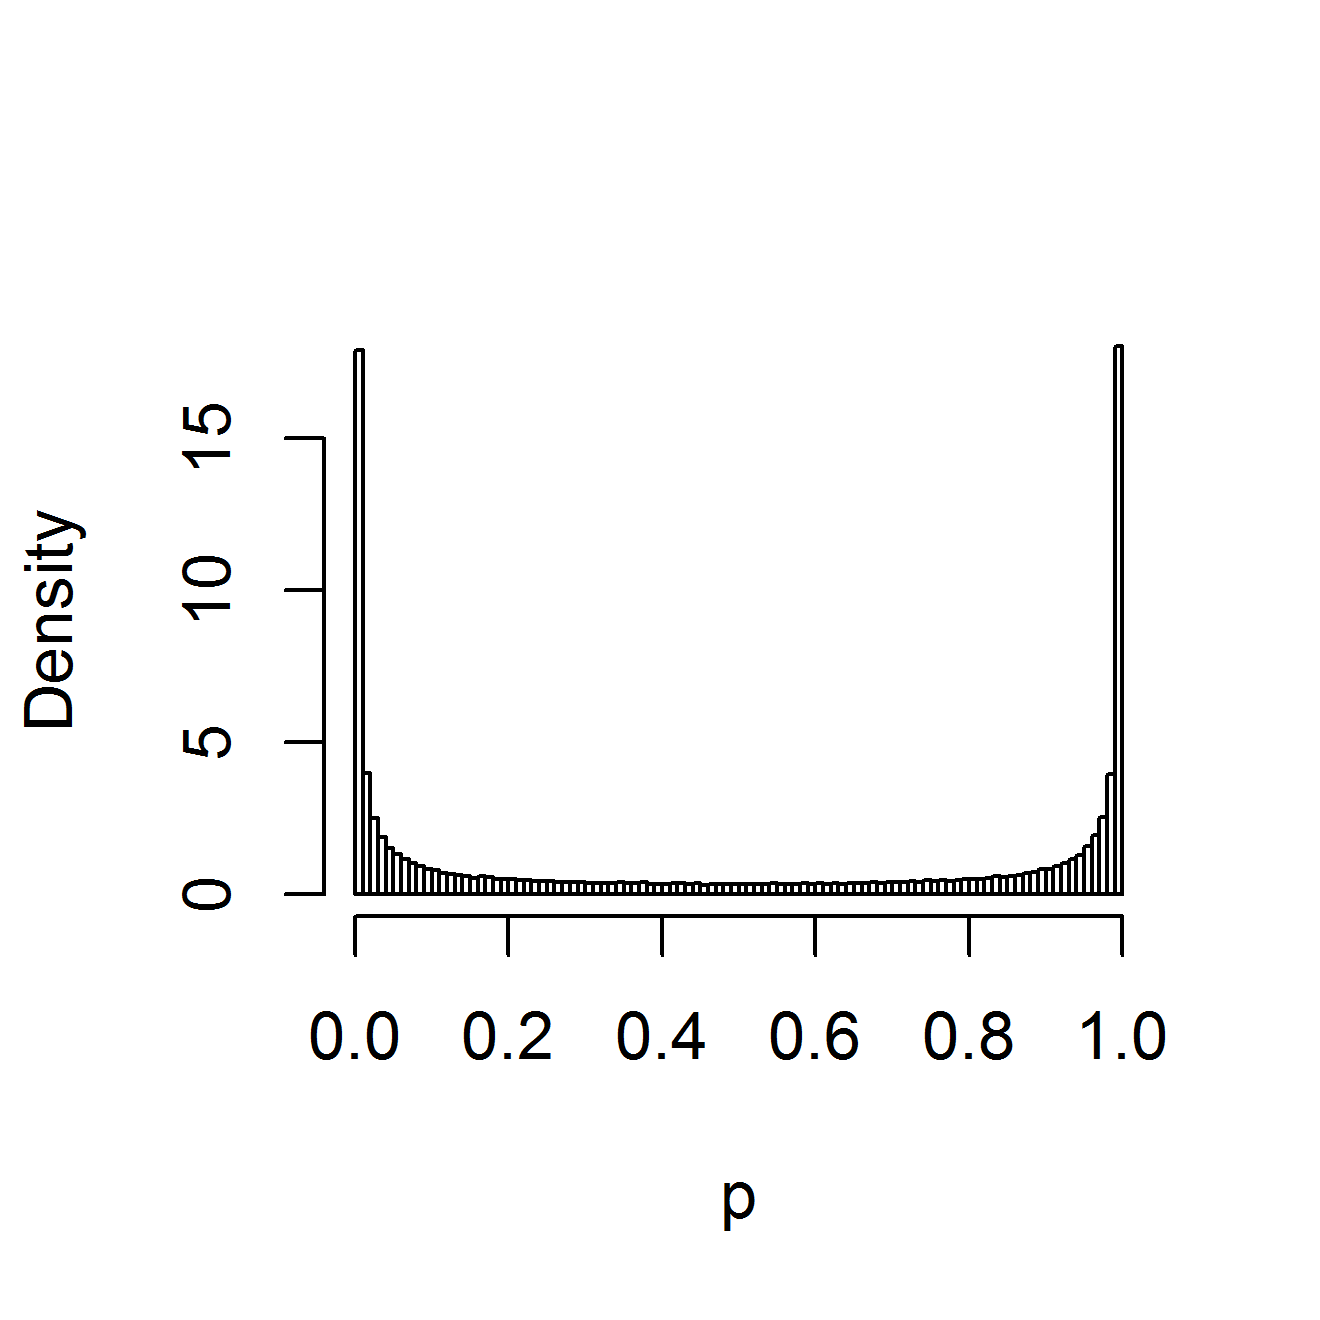
\includegraphics[height=3.3in]{Ch2/figs/implied_prior}
\end{center}
\caption{Implied prior for $p_{0} = exp(\beta_0)/(1+exp(\beta_0))$ 
if $\beta_0 \sim \mbox{Normal}(0, 5^2)$.}
\label{glms.fig.impliedprior}
\end{figure}
These two priors can
affect results (see Chapt. \ref{chapt.closed} sec. XXXXX), yet they are both 
sensible
non-informative priors. Choice of priors and parameterization is
very much problem-specific and often largely subjective. Moreover, it
also affects the behavior of MCMC algorithms and therefore the analyst
needs to pay some attention to this issue and possibly try different
things out.
Most standard Bayesian analysis books address issues related to specification and
affect of prior distribution choice in some depth. Some good references include 
\citet{kass_wasserman:1996}, \citet{gelman:2006} and \citet{link_barker:2010}.


\subsection{Convergence and so-forth}
\label{glms.sec.convergence}

Once we have carried-out an analysis by MCMC, there are many other
practical issues that we have to confront. One characteristic of MCMC sampling is that Markov chains take some time to converge to their stationary distribution - in our case the posterior distribution for some parameter, given some data, $\theta|y$. Only when the Markov chain has reached
its stationary distribution, the generated samples can be used to
characterize the posterior distribution. Thus, one of the most important issues we need to address 
is ``have the chains converged?'' Since we do not know what the
stationary posterior distribution of our Markov chain should look like
(this is the whole point of doing an MCMC approximation), we
effectively have no means to assess whether it has truly converged to
this desired distribution or not. Most MCMC algorithms only guarantee
that, eventually, the samples being generated will be from the target
posterior distribution, but no-one can tell us how long this will
take. Also, you only now the part of your posterior distribution that
the Markov chain has explored so far -- for all you know the chain
could be stuck in a local maximum, while other maxima remain
completely undiscovered.  Acknowledging that there is truly nothing we
can do to ever prove convergence of our MCMC chains, there are several
things we can do to increase the degree of confidence we have about
the convergence of our chains. Some problems are easily detected using
simple plots.  Typically a period of transience is observed in the
early part of the MCMC algorithm, and this is usually discarded as the
``burn-in'' period. The quick diagnostic to whether convergence has
been achieved is that your Markov chains look ``grassy'' -- see Fig.
\ref{glms.fig.grassy} below.  Another way to check convergence is to
update the parameters some more and see if the posterior changes. Yet
another option, and one generally implemented in {\bf WinBUGS}, is to
run several Markov chains and to start them off at different initial
values that are overdispersed relative to the posterior
distribution. Such initial values help to explore different areas of
the parameter space simultaneously; if after a while all chains
oscillate around the same average value, chances are good that they
indeed converged to the posterior distribution. \footnote{Running
  several parallel chains is computationally expensive. But extra
  computational demands are not the only and by no means the major
  concern some people voice when it comes to running several parallel
  MCMC chains to assess convergence. Again, consider the fact that we
  do not know anything about the true form of the posterior
  distribution we are trying to approximate. How do we, then, know how
  to pick overdispersed initial values? We don't. All we can do is
  pick overdispersed values relative to our expectations of what the
  posterior should look like. To use a quote from the home page of
  Charlie Geyer, a Bayesian statistician from the University of
  Minnesota, ``If you don't know any good starting points [...], then
  restarting the sampler at many bad starting points is [...] part of
  the problem, not part of the solution.''
  (\url{''http://users.stat.umn.edu/~charlie/mcmc/diag.html''}). His suggestion
  is that your only chance to discover a potential problem with your
  MCMC sampler is to run it for a very long time. But again, there is
  no way of knowing how long is long enough.  It is up to you to
  decide, which school of thoughts appeals more to you, one long
  versus several parallel Markov chains. Irrespectively, part of
  developing an MCMC sampler should be to make sure (within reasonable
  limits) that you are not missing regions of high posterior density
  because of the way you specify your starting values. Once you have
  explored the behavior of your chain under a reasonable range of
  starting values, you may feel comfortable enough to run only one
  long chain.} Gelman and Rubin came up with the so-called``R-hat''
statistic ($\hat{R}$) or Brooks-Gelman-Rubin statistic that
essentially compares within-chain and between-chain variance to check
for convergence of multiple chains \citep{gelman_etal:1996}. $\hat{R}$
should be close to 1 if the Markov chains have converged and
sufficient posterior samples have been obtained. In practice, $\hat{R}
= 1.2$ is probably good enough for some problems.  For some models you
can't actually realize a low $\hat{R}$. E.g., if the posterior is a
discrete mixture of distributions then you can be misled into thinking
that your Markov chains have not converged when in fact the chains are
just jumping back and forth in the posterior state-space.
%So, for example, model
%selection methods (section XYZ) sometimes suggests non-convergence.
Another situation is when one of the parameters is on the boundary of
the parameter space which might appear to be very poor mixing, but all
within some extreme region of the parameter space.\footnote{it would
  be nice if we could compile examples of this later in the book and
  reference back to this point}.
This
kind of stuff is normally ok and you need to think really hard about
the context of the model and the problem before you conclude that your
MCMC algorithm is ill-behaved.

Some models exhibit ``poor mixing'' of the Markov chains (or ``slow convergence'')
in which case the samples might well
be from the posterior (i.e., the Markov chains have converged to the
proper stationary distribution) but simply mix around the posterior
rather slowly. Anyway, poor mixing can happen for many
reasons -- when parameters are highly correlated (even confounded), or
barely identified from the data, or the algorithms are very terrible
and probably many others.  Slow mixing equates to high
autocorrelation in the Markov chain - the successive draws are highly
correlated, and thus we need to run the MCMC algorithm much longer to
get an effective sample size that is sufficient for estimation, or to
reduce the MC error (see below) to a tolerable level.  A strategy often used to
reduce autocorrelation is ``thinning'' - i.e., keep only every $m^{th}$
value of the Markov chain output. However, thinning is necessarily
inefficient from the stand point of inference - you can always get
more precise posterior estimates by using all of the MCMC output
regardless of the level of autocorrelation
\citep{maceachern_berliner:1994, link_eaton:2011}. Practical considerations might
necessitate thinning, even though it is statistically inefficient. For
example, in models with many parameters or other unknowns being
tabulated, the output files might be enormous and unwieldy to work
with. In such cases, thinning is perfectly reasonable. In many cases,
how well the Markov chains mix is strongly influenced by
parameterization, standardization of covariates, and the prior
distributions being used. Some things work better than others, and the
investigator should experiment with different settings and
remain calm when things don't work out perfectly. MCMC is an
art, as much as it is a science.


{\bf Is the posterior sample large enough?}  The subsequent samples
generated from a Markov chain are not {\it iid} samples from the
posterior distribution, due to the correlation amongst samples
introduced by the Markov process\footnote{In case you are not familiar with Markov chains, for
  $T$ random samples $\theta^ {(1)}$, ... $\theta^{(T)}$ from a Markov chain
  the distribution of $\theta^{(t)}$ depends only on the immediately preceding
  value, $\theta^{(t-1)}$.} and the sample size has to be
adjusted to account for the autocorrelation in subsequent samples (see
Chapt. 8 in \citet{robert_casella:2010} for more details). This
adjusted sample size is referred to as the effective sample
size. Checking the degree of autocorrelation in your Markov chains and
estimating the effective sample size your chain has generated should
be part of evaluating your model output. {\bf WinBUGS} will
automatically return the effective sample size for all monitored
parameters. If you find that your supposedly long Markov chain has
only generated a very short effective sample, you should consider a
longer run. What exactly constitutes a reasonable effective sample
size is hard to say. A more palpable measure of whether you've run
your chain for enough iterations is the time-series or Monte Carlo
error - the 'noise' introduced into your samples by the stochastic
MCMC process. The MC error \index{Monte Carlo error} is printed by
default in summaries produced in the {\bf WinBUGS} GUI, and using the
\mbox{\tt summary} command applied to {\bf JAGS} output (MC error is called
Time-series SE in {\bf JAGS}). You want that to be
smallish relative to the magnitude of the parameter and what smallish means will
depend on the purpose of the analysis. For a preliminary analysis you
might settle for a few percent whereas for a final analysis then
certainly less than 1\% is called for, but you can run your MCMC
algorithm as long as it takes. A consequence of the MC error is that
even for the exact same model, results will always be different. Thus,
as a good rule of thumb you should never report MCMC results to more
than 2 decimal places.
\begin{comment}
% another attempt to address this issue ineffectively 
Note that MC error in summaries of the
posterior is not the same as having an ``approximate'' solution in a
standard likelihood analysis or similar.  The approximate SE in
likelihood inference is actually wrong in its actual value.... XYZ.
\end{comment}

\subsection{Bayesian confidence intervals}

The 95\% Bayesian confidence interval based on percentiles of the posterior
is not a unique interval - there are many of them - and the so-called
``highest posterior density'' (HPD) interval is the narrowest
interval. We might compute that frequently because it is easy to do
with an integer parameter which $N$ is (see the next chapter). The
95 \% HPD is not often exactly 95\% but usually slightly more
conservative than nominal because it is the narrowest interval that
contains at least 95\%  of the posterior mass.

\subsection{Estimating functions of parameters}

A benefit of analysis by MCMC is that we can seamlessly estimate
functions of parameters by simply tabulating the desired function of
the simulated posterior draws. For example, if $\theta$ is the
parameter of interest and let $\theta^{(i)}$ for $i=1,2,\ldots,M$ be
the posterior samples of $\theta$. Let $\eta = exp(\theta)$, then a
posterior sample of $\eta$ can be obtained simply by computing
$exp(\theta^{(i)})$ for $i=1,2,\ldots,M$. We give another example in
section
\ref{glms.sec.xopt}
below and throughout this book.
Almost all SCR models in this book involve at least 1 derived
parameter. For example, density $D$ is a derived parameter, being a
function of population size $N$ and the area $A$ of the underlying
state-space of the point process (see Chapt. \ref{chapt.scr0}).

\section{Bayesian Analysis using the BUGS language}

We won't be too concerned with devising our own MCMC algorithms for
every analysis
although we will do that a few times for fun.  More often, we
will rely on the freely available software package {\bf WinBUGS} or
{\bf JAGS}
for doing this.  We will always execute these {\bf BUGS} engines from
within {\bf R} using the \mbox{\tt R2WinBUGS} \citep{sturtz_etal:2005}
or 
\mbox{\tt rjags} \citep{plummer:2009} packages. 
{\bf WinBUGS} and {\bf JAGS} are  MCMC black boxes
that takes a pseudo-code description (i.e., the {\bf BUGS}
language) of all of the relevant stochastic
and deterministic elements of a model and generate an MCMC algorithm
for that model. But you never get to see the algorithm. Instead,
{\bf WinBUGS}/{\bf JAGS} will run the 
algorithm and  return the Markov chain output
- the posterior samples of model parameters.

The great thing about using the {\bf BUGS} language is that it forces
you to become intimate with your statistical model - you have to write
each element of the model down, admit (explicitly) all of the various
assumptions, understand what the actual probability assumptions are
and how data relate to latent variables and data and latent variables
relate to parameters, and how parameters relate to one another.

While we normally use
{\bf WinBUGS}, we note that {\bf
 OpenBUGS} is the current active development tree of the {\bf BUGS}
project. See \citet[][ch.xyz]{kery:2010} and
\citet[][appendix xyz]{kery_schaub:2011} for more on practial analysis
in {\bf WinBUGS}. We also frequently use {\bf JAGS}, and you can refer to \citet{hobbs:2011} for an ecological
perspective on {\bf JAGS}.
That book should also be consulted
for a more comprehensive introduction to using {\bf WinBUGS}. In this
example, we're going to accelerate pretty fast.

\subsection{Linear Regression in WinBUGS}

We provide a brief introductory example of a normal regression model
using a small simulated data set. The following commands are executed
from within your {\bf R} workspace.
First, simulate a covariate $x$ and observations $y$ having
prescribed intercept, slope and variance:
\begin{verbatim}
 x<-rnorm(10)
 mu<- -3.2+ 1.5*x
 y<-rnorm(10,mu,sd=4)
\end{verbatim}
The {\bf BUGS} model specification for a normal regression model is
written within {\bf R} as a character string input to the command
\mbox{\tt cat()} and
then dumped to a text file named \mbox{\tt normal.txt}:
\begin{verbatim}
cat("
 model {
   for (i in 1:10){
      y[i]~dnorm(mu[i],tau)        # the "likelihood"
      mu[i]<- beta0 + beta1*x[i]   # the linear predictor
     }
   beta0~dnorm(0,.01)              # prior distributions
   beta1~dnorm(0,.01)
   sigma~dunif(0,100)
   tau<-1/(sigma*sigma)            # tau is a derived parameter
}
",file="normal.txt")
\end{verbatim}
Alternatively, you
can write the model specifications directly within a text file and
save it in your current working directory, but we do not usually take
that approach in this book.

The {\bf BUGS} dialects parameterize the normal 
distribution in
terms of the mean and inverse-variance, called the precision. Thus,
\mbox{\tt dnorm(0,.01)} implies a variance of 100.
We typically use diffuse normal priors for mean parameters, $\beta_0$ and $\beta_1$ in this case, but sometimes we might use uniform priors with suitable bounds -B and +B.
Also, we typically use a $\text{Uniform}(0,B)$ prior on standard
deviation parameters
\citep{gelman:2006}.
But sometimes we might use a gamma prior on the precision parameter $\tau$.
In a {\bf BUGS} model file, every variable referenced in
the model description has to be
either data, which will be input (see below), a random variable which
must have a probability distribution associated with it using the
tilde character (aka ``twiddle'') ``\verb#~#'', or it has to be a derived parameter connected to variables and
data using ``\mbox{\tt <-}''.


To fit the model, we need to describe various data objects to {\bf
  WinBUGS}. In particular,
we create an {\bf R} list object called \mbox{\tt data} which
are the data objects identified in the {\bf BUGS} model file.
 In the example, the
data consist of two objects which exist as $y$ and $x$ in the {\bf R}
workspace and also in the {\bf WinBUGS} model definition.
 We also have to create an {\bf R} function
that produces a list of starting values, \mbox{\tt inits}, that get sent to
{\bf WinBUGS}.
 Finally, we identify
the names of the parameters (labeled correspondingly in the {\bf WinBUGS}
model specification) that we want {\bf WinBUGS} to save the MCMC output
for. In this example, we will ``monitor'' the parameters
$\beta_0$, $\beta_1$, $\sigma$ and $\tau$.
{\bf WinBUGS} is executed using the {\bf R} command
\mbox{\tt bugs()}.
We set the option \mbox{\tt debug=TRUE} if we want the {\bf WinBUGS}
GUI to stay open (useful for analyzing MCMC output and looking at the
{\bf WinBUGS} error log). Also, we set \mbox{\tt working.dir=getwd()}
so that {\bf WinBUGS} output files and the log file are saved in the
current {\bf R} working directory.
  All of these activities look like this:
{\small
\begin{verbatim}
 library("R2WinBUGS")    # "attach" the R2WinBUGS library
 data <- list ( "y","x")
 inits <- function()
  list ( beta1=rnorm(1),beta0=rnorm(1),sigma=runif(1,0,2) )
 parameters <- c("beta0","beta1","sigma","tau")
 out<-bugs (data, inits, parameters, "normal.txt", n.thin=2, n.chains=2,
             n.burnin=2000, n.iter=6000, debug=TRUE,working.dir=getwd())
\end{verbatim}
}

A common question is ``how should my data be
formatted?'' That depends on how you describe the model in the {\bf
  BUGS} language, and how your data are input into {\bf R}.
 There is no unique way to describe any
particular model and so you have some flexibility. We talk about data
format further in the context of capture-recapture models and SCR
models in Chapt. \ref{chapt.scr0} and elsewhere.  In general,
starting values are optional. We recommend to always provide
reasonable starting values for structural parameters, but not
necessarily for random effects\footnote{While {\bf WinBUGS} is reasonably robust to a wide rangin of more or less plausible startign values, {\bf JAGS} is a lot more sensitive and especially with more complex models you might actually have to spend some time thinking about how to specify good starting values to get the model running \ref{chapt.app1}; we will come back to this issue when we use {\bf JAGS}}.  Note that the previously created
objects defining data, initial values and parameters to monitor are
passed to the function \mbox{\tt bugs()}.  In addition, various other
things are declared: The number of parallel Markov chains (\mbox{\tt
  n.chains}), the thinning rate (\mbox{\tt n.thin}),
the number of burn-in iterations (\mbox{\tt n.burnin}) and the total
number of iterations
(\mbox{\tt n.iter}).
To develop a detailed understanding of the various parameters and
settings used for MCMC, consult a basic reference such as
\citet{kery:2010}.



You should execute all of the commands given above and then look at
the resulting output (summarized in table \ref{}). Close the {\bf WinBUGS} GUI and the data will be
read back into {\bf R} (or specify \mbox{\tt debug=FALSE}).  We don't
want to give instructions on how to navigate and use the GUI - but you
can fire up {\bf WinBUGS} and read the help files, or see Ch. 4 from
\citet{kery:2010} for a brief introduction.
The object \mbox{\tt out} prints important
summaries by default (this is slightly edited):

{\small
\begin{verbatim}
> print(out,digits=2)
Inference for Bugs model at "normal.txt", fit using WinBUGS,
 2 chains, each with 6000 iterations (first 2000 discarded), n.thin = 2
 n.sims = 4000 iterations saved
          mean   sd  2.5%   25%   50%   75% 97.5% Rhat n.eff
beta0    -2.43 1.84 -6.21 -3.50 -2.42 -1.34  1.27    1  4000
beta1     2.62 1.54 -0.42  1.68  2.62  3.57  5.67    1  4000
sigma     5.29 1.66  3.11  4.14  4.95  6.05  9.39    1  4000
tau       0.05 0.02  0.01  0.03  0.04  0.06  0.10    1  4000
deviance 59.85 3.24 56.18 57.47 59.00 61.37 68.32    1   840

For each parameter, n.eff is a crude measure of effective sample size,
and Rhat is the potential scale reduction factor (at convergence, Rhat=1).

DIC info (using the rule, pD = Dbar-Dhat)
pD = 2.6 and DIC = 62.4
\end{verbatim}
}

 In the {\WinBUGS} output you see a column called ``Rhat''. This is the $\hat{R}$ statistic we introduced in \ref{glms.sec.convergence} to check whether the multiple chains converged (a value near 1 indicates satisfactory convergence). DIC is the
``deviance information criterion'' \citep{spiegelhalter_etal:2002}
(see section \ref{glms.sec.modsel})
 which
some people use in a manner similar to AIC although it is recognized
to have some problems in hierarchical models \citep{millar:2009}. We
evaluate this in the context of SCR models in Chapt. \ref{chapt.gof}.

%Richard will move and write this section into Ch2
\subsection{Modeling categorical variable effects with dummy
  variables}
\label{glms.sec.dummy}

Make point here that we often have categorical variables -- with
nominal levels these are ``factors'', and we model these using dummy
variables but sometimes in \bugs we use ``index variables''.
%end of section Richard will develop in Ch2


\subsection{Inference about functions of model parameters}
\label{glms.sec.xopt}

Using the MCMC draws for a given model we can easily obtain the
posterior distribution of any function of model parameters.  We showed
this in the above example by providing the posterior of $\tau$ when
the model was parameterized in terms of standar deviation $\sigma$.
 As another example, suppose that the
normal regression model above had a quadratic response function of the
form
\[
	E(y_i) = \beta_0 + \beta_1 x_i + \beta_2 x_{i}^{2}
\]
Then the optimum value of $x$, i.e., that corresponding to the optimal
expected response, can be found by setting the derivative of
this function to 0 and solving for $x$. We find that
\[
df/dx = \beta_1 +
2*\beta_2 x = 0
\]
yields that $x_{opt} = -\beta_1/(2*\beta_2)$.  We can just
take our posterior draws for $\beta_1$ and $\beta_2$ and obtain a
posterior sample of $x_{opt}$ by this simple calculation applied to
the posterior output. As an exercise, take
the normal model above and simulate a quadratic response and then
describe the posterior distribution of $x_{opt}$.


\section{Model Checking and Selection}
\label{glms.sec.modsel}

In general terms model checking - or assessing the adequacy of the
model - and model selection are quite thorny issues and, despite
contrary and, sometimes, strongly held belief among practitioners, there are not
really definitive, general solutions to either problem. We're against
dogma on these issues and think people need to be open-minded about
such things and recognize that models can be useful whether or not
they pass certain statistical tests. Some models are intrinsically
better than others because they make more biological sense or foster
understanding or achieve some objective that some  bootstrap
or other goodness-of-fit test can't decide for you. That said, it
gives you some confidence if your model seems adequate in a purely statistical
sense and we try to
provide some fit assessment in most real applications of SCR models.
We provide a very brief overview of concepts here, but provide more
detailed coverage in Chapt. \ref{chapt.gof}.
See also
\citet[][ch. xyz]{kery:2010} and
\citet[][ch. xyz]{link_barker:2009}
for specific context related to Bayesian
model checking and selection.

\subsection{Goodness-of-fit}
\label{glms.sec.gof}

Goodness-of-fit testing is an important element of any analysis
because  our model represents a general set of hypotheses
about the ecological and observation processes that generated our
data. Thus, if our model ``fits'' in some statistical or scientific
sense, then we believe it to be consistent with the hypotheses that
went into the model. More formally, we would conclude that the data
are {\it not inconsistent} with the hypotheses, or that the model
appears adequate. If we have enough
data, then of course we will reject any set of statistical hypotheses.
Conversely, we can always come up with a model that fits by making the
model extremely complex. Despite this paradox, it seems to us that
simple models that you can understand should usually be preferred even
if they don't fit, for example if they embody essential mechanisms
central to our understanding of things, or
if we think that some contributing factors to lack-of-fit are minor or
irrelevant to the scientific context and intended use of the model.
In other words, models can be useful irrespective of whether they fit
according to some formal statistical test of fit.  Yet
the tension is there to obtain fitting models, and this comes naturally at
the expense of models that can be easily interpreted and studied and
effectively used.
Unfortunately, conducting a goodness-of-fit test is
not always so easy to do. And, moreover, it is never really easy (or
especially convenient) to decide if your goodness-of-fit test is worth
anything. It might have 0 power!
Despite this,
we recommend attempting to assess model fit in real applications,
as a general rule, and we provide some basic guidance here and some more
specific to SCR models in
Chapt. \ref{chapt.gof}.

To evaluate goodness-of-fit in Bayesian analyses, we will most often
use the Bayesian p-value \citep{gelman_etal:1996}.  The basic idea is to define
a fit statistic or ``discrepancy measure'' and compare the posterior distribution of that
statistic to the posterior predictive distribution of that statistic
for hypothetical perfect data sets for which the model is known to be correct. For
example, with count frequency data, a standard measure of fit is the
sum of squares of the ``Pearson residuals'',
\[
D(y_i,\theta) = \frac{(y_i - E(y_i))^{2}}{\sqrt{V( y_{i} )}}
\]
The fit statistic based on the squared residuals computed from the
observations is 
\[
T({\bf y}, \theta) = \sum_{i} D(y_{i},\theta)^{2}
\]
which can be computed at each iteration of a MCMC algorithm given the
current values of parameters that determine the
 response distribution.  At the same time (i.e., at each MCMC
 iteration),
the equivalent statistic is computed for a
``new'' data set, say ${\bf y}^{new}$, 
simulated using the current parameter values. From the new data set,
we compute the same fit statistic:
\[
T({\bf y}^{new}, \theta) = \sum_{i} D(y_{i}^{new},\theta)^{2}
\]
and 
the
Bayesian p-value is simply the posterior probability $\Pr(T({\bf
  y}^{new})  >  T({\bf y}))$
 which should be close to $0.50$ for a good model -- one that
 ``fits'' in the sense that the observed data set is
 consistent with realizations simulated under the model being fitted
 to the observed data. In practice
we judge ``close to 0.50'' as being ``not too close to 0 or 1'' and,
as always, closeness is somewhat subjective. We're happy with anything
$>.1$ and $<.9$ but might settle for $>.05$ and $<0.95$. 
Another useful fit statistic is the Freeman-Tukey
statistic, in which
\[
D({\bf y},\theta) = \sum_{i} ( \sqrt{y_{i}} - \sqrt{e_{i}} )^2
\]
\citep{brooks_etal:2000}, where $y_{i}$ is the observed value of
observation $i$ and $e_{i}$ its expected value. In contrast to a
Chi-square discrepancy, the Freeman-Tukey statistic removes the need
to pool cells with small expected values.
In summary, you can see that 
the Bayesian p-value is easy to compute,
and it is widely used as a result.


\subsection{Model Selection }

In ecology, scientific hypotheses are often manifest as different models or parameters
 of a model, and so
evaluating the importance of different models is fundamental 
to many ecological studies.
For model selection we typically use three different methods: First
is, let's say, common sense. If a parameter has posterior mass
concentrated away from 0 then it seems like it should be regarded as
important - that is, it is ``significant.''  This approach seems to
have fallen out of favor with all of the interest over the last 10 or
15 years on model selection in ecology. It seems reasonable to us.


For regression problems we sometimes use the factor weighting idea
which is to introduce a set of binary variables $w_{k}$ for variable
$k$, and express the model as, e.g., for a single covariate model:
 \[
 E(y_i) = \beta_0 + w \beta_1 x_{i}
\]
where $w$ is given a Bernoulli prior distribution with some prescribed
probability. E.g., $w \sim Bern(0.50)$ to provide a prior probability
of 0.50 that variable $x$ should be an element of the linear
predictor. The posterior probability of the event $w=1$ is a gauge of
the importance of the variable $x$. i.e., high values of $\Pr(w=1)$
indicate stronger evidence to support that ``$x$ is in the model''
whereas values of $\Pr(w=1)$ close to 0 suggest that $x$ is less
important.



This idea seems to be due to \citet{kuo_mallick:1998} and see
\citet[][Chapt. 3]{royle_dorazio:2008} for an example in the context
of logistic regression. This approach seems to even work sometimes
with fairly complex hierarchical models of a certain form. E.g.,
\citet{royle:2008} applied it to a random effects model to evaluate
the importance of the random effect component of the model.  The main
problem with this approach is that its effectiveness and results will
typically be highly sensitive to the prior distribution on the
structural parameters (e.g., see \citet[][table xyz]{royle_dorazio:2008}).
The reason for this is obvious: If $w = 0$ for the current
iteration of the MCMC algorithm, so that $\beta$ is sampled from the
prior distribution, and the prior distribution is very diffuse, then
extreme values of $\beta$ are likely. Consequently, when the current value of
$\beta$ is
far away from the mass of the posterior when $w=1$, then the Markov
chain may only jump from $w=0$ to $w=1$ infrequently.  One seemingly
reasonable solution to this problem \citep{aitkin:1991}
is to fit the full
model to obtain posterior distributions for all parameters, and then
use those as prior distributions in a ``model selection'' run of the
MCMC algorithm.  This seems preferable to more-or-less arbitrary restriction of
the prior support to improve the performance of the MCMC algorithm.

A third method that that we advocate is subject-matter
context. It seems that there are some situations -- some models -- where one should not
have to do model selection because it is necessitated by the specific
context of the problem, thus rendering a formal hypothesis test pointless
\citep{johnson:1999}.
SCR models are such an example. In SCR models, we will see that
``spatial location'' of individuals is an element of the model. The
simpler, reduced, model is an ordinary capture-recapture model which
is not spatially explicit (i.e., Chapt. \ref{chapt.closed}),
but it seems silly and pointless to think about actually using the
reduced model even if we could concoct some statistical test to refute
the more complex model.  The simpler model is manifestly wrong but,
more importantly, not even a plausible data-generating model!
Other examples are when effort, area or
sample rate is used as a covariate. One might prefer to have such things in
models regardless of whether or not they pass some statistical litmus
test (although one can always find referees to argue for pedantic procedure
over thinking).


Many problems can be approached using one of these methods but there
are also broad classes of problems that can't and, for those, you're
on your own. In later chapters we will address model selection in
specific contexts and we hope those will prove useful for a majority
of the situations you encounter.


\section{Poisson GLMs}
\label{glms.sec.poisson}

The Poisson GLM (also known as ``Poisson regression'') is probably the
most relevant and important class of models in all of ecology. The
basic model assumes observations $y_{i}; i=1,2,...,n$ follow a Poisson
distribution with mean $\lambda$ which we write
\[
 	y_{i} \sim \mbox{Poisson}(\lambda)
\]
Commonly $y_{i}$ is a count of animals or plants at some point in
space $i$, and $\lambda$ might depend on $i$. For example, $i$ might index point
count locations in a forest, BBS route centers, or sample quadrats, or
similar.  If covariates are available it is typical to model them as
linear effects on the log mean. If $x_i$ is some measured covariate
associated with observation $i$. Then,
\[
 	log(x_i) = \beta_0  + \beta_1 x_i
\]

While we only specify the mean of the Poisson model directly, the
Poisson model (and all GLMs) has a ``built-in'' variance which is
directly related to the mean. In this case, $\mbox{Var}(y) = \mbox{E}(y) =
\lambda$. Thus the model accommodates a linear increase in variance
with the mean.

%Richard: move to Ch2
\subsection{Important properties of the Poisson distribution}
\label{glms.sec.properties}

There are two properties of the Poisson distribution
that make it extremely useful in ecology. First
is the property of {\it compound additivity}. If $y_1$ and $y_2$ are
Poisson random variables with means $\lambda_1$ and $\lambda_2$,
then their sum $N=y_1+y_2$ is Poisson with mean $\lambda_1+\lambda_2$. Thus,
if the observations can be viewed as an aggregate of counts over some
finer unit of measurement, then the Poisson mean aggregates in a corresponding
manner. This comes in hand in some ecological applications
where we have counts, $y_{i}$, made on sample units with different but known areas $A_{i}$. 
Then, we might assume 
the counts have a Poisson distribution with mean $A_{i}\lambda$. On the log-scale we see that 
$log(A_{i})$ enters as an additive constant -- usually referred to as the ``offset'' in GLM
lingo. 
A second useful property of the Poisson distribution is its
direct relationship to the multinomial.
If $y_1$ and $y_2$ are $iid$ Poisson then,
conditional on their sum $N = y_1 + y_2$, their joint distribution is multinomial
 with sample size $N$ and cell probabilities
$\lambda_1/(\lambda_1+\lambda_2)$ and
$\lambda_2/(\lambda_1+\lambda_2)$.  As a result of this, most
multinomial models can be analyzed as a Poisson GLM and {\it vice versa}.
%END section moved to Ch2

\subsection{Example: Breeding Bird Survey Data}

As an example we consider a classical situation in ecology where
counts of an organism are made at a collection of spatial
locations. In this particular example, we have mourning dove counts
made along North American Breeding Bird Survey (BBS) routes in
Pennsylvania, USA. A route consists of 50 stops separated by 0.5
mile. For the purposes here we are defining $y_i$ = route total count
and the sample location will be marked by the center point of the BBS
route.  The survey is run annually and the data set we have is
1966-1998. BBS data can be obtained online at \mbox{\tt http:\//\//www.pwrc.usgs.gov\//bbs\//}, but the particulart chunk of data we will be using here is also included in the {\tt scrbook} package ({\tt bbsdata}).
We will make use of the whole data set shortly but for now we're going
to focus on a specific year of counts -- 1990 -- for the sake of
building a simple model.
 For 1990 there were 77 active routes, where rows index the unique route, column 1 is the
route ID, columns 2-3 are the route coordinates (longitude/latitude),
column 4 is a habitat covariate ``forest cover'' (standardized, see
below) and the remaining columns are the yearly counts. Years for
which a route was not run are coded as ``\mbox{\tt NA}'' in the data matrix. We
imagine that this will be a typical format for many ecological
studies, perhaps with more columns representing covariates.  To read
in the data and display the first few elements of the data frame containing the counts, do
this:
{\small
\begin{verbatim}
data(bbsdata) #loads data frame 'bbs'
bbsdata$counts[1:2,1:6]
      X     lon    lat    habitat X66 X67
1 72002 -80.445 41.501 -0.3871372  NA  24
2 72003 -80.347 41.214 -1.0171629  NA  NA
\end{verbatim}
}

It is useful to display the spatial pattern in the observed counts. For that we use a
spatial dot plot - where we plot the coordinates of the observations
and mark the color of the plotting symbol based on the magnitude of
the count.  We have a special plotting function for that which is
called \mbox{\tt spatial.plot()} and it is available with the
supplemental {\bf R} package.
Actually, what we want to do here is plot the
log-counts (+1 of course) which (Fig. \ref{glms.fig.padovecounts}) display a notable pattern that could
be related to something. The {\bf R} commands for obtaining this figure are:
{\small
\begin{verbatim}
data(bbsdata)
y<-bbsdata$counts[,29]  # pick out 1990
notna<-!is.na(y)
y<-y[notna]
spatial.plot(bbsdata$counts[notna,2:3],y)
\end{verbatim}
}
 We can ponder the potential effects that
might lead to dove counts being high....corn fields, telephone wires,
barn roofs along with misidentification of pigeons, these could all
correlated reasonably well with the observed count of mourning doves.
Unfortunately we don't have any of that information.

\begin{figure}
\begin{center}
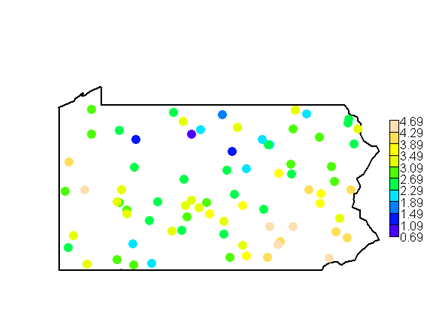
\includegraphics[height=2.75in]{Ch2/figs/PA1}
\end{center}
\caption{Plot of log-counts of mourning doves along North American Breeding Bird Survey routes in Pennsylvania (data from 1990).}
\label{glms.fig.padovecounts}
\end{figure}

We do have a measure of forest cover in the vicinity of each point
which is contained in the data set (variable ``habitat''). This was derived
from a larger GIS coverage of the state (provided in the data frame
``\mbox{\tt bbsdata\$habitat}'') which can be plotted using the \mbox{\tt spatial.plot} function
using the following commands
{\small
\begin{verbatim}
library(maps)
habdata<-bbsdata$habitat
map('state',regions="penn",lwd=2)
spatial.plot(habdata[,2:3],habdata[,"dfor"],cx=2)
map('state',regions="penn",lwd=2,add=TRUE)
\end{verbatim}
}
where the result appears in Fig. \ref{glms.fig.paforest}.
We see a prominent pattern that indicates high forest coverage in the
central part of the state and low forest cover in the SE.  Inspecting
the previous figure of log-counts suggests a relationship between
counts and forest cover which is perhaps not surprising.
\begin{figure}
\begin{center}
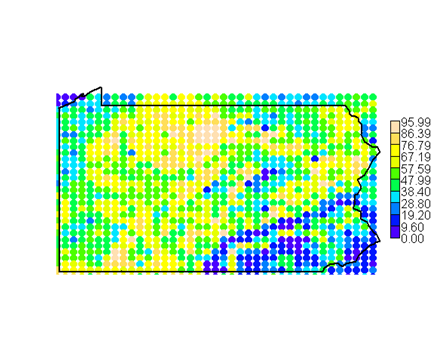
\includegraphics[height=2.75in]{Ch2/figs/PA2}
\end{center}
\caption{Plot of forest cover in Pennsylvania.}
\label{glms.fig.paforest}
\end{figure}

\subsection{Doing it in WinBUGS}

Here we demonstrate how to fit a Poisson GLM in {\bf WinBUGS} using the
covariate $x_{i} =$ forest cover. It is advisable that $x_i$ be
standardized in most cases as this will improve mixing of the Markov
chains. Recall that the data we have stored include a standardized
covariate (forest cover) and so we don't have to worry about that
here.  To read the BBS data into {\bf R} and get things set up for
{\bf WinBUGS}
we issue the following commands:
{\small
\begin{verbatim}
data(bbsdata)
data<-bbsdata$counts                        # pick out 1990
notna<-!is.na(y)
y<-y[notna]                         # discard missing
habitat<-data[notna,4]              # get habitat data
library("R2WinBUGS")                # load R2WinBUGS
data <- list ( "y","M","habitat")   # bundle data for WinBUGS
M<-length(y)
\end{verbatim}
}
Now we write out the Poisson model specification in {\bf WinBUGS}
pseudo-code, provide initial values, identify parameters to be
monitored and then execute {\bf WinBUGS}:
{\small
\begin{verbatim}
cat("
model {
    for (i in 1:M){
      y[i]~dpois(lam[i])
      log(lam[i])<- beta0+beta1*habitat[i]
     }
 beta0~dunif(-5,5)
 beta1~dunif(-5,5)
}
",file="PoissonGLM.txt")

inits <- function()  list ( beta0=rnorm(1),beta1=rnorm(1))
parameters <- c("beta0","beta1")
out<-bugs (data, inits, parameters, "PoissonGLM.txt", n.thin=2,n.chains=2,
                n.burnin=2000,n.iter=6000,debug=TRUE,working.dir=getwd())
\end{verbatim}
}
Note the close correspondence in how the model is
specified here compared with the normal regression model
previously. As an exercise you should discuss the specific differences
between the {\bf BUGS} model specifications for the normal and Poisson
models. 

% Model output is summarized in table \ref{glms.tab.poisreg}. 
% \begin{table}
% \caption{Inference for Poisson GLM, fit using WinBUGS,
%  2 chains, each with 6000 iterations (first 2000 discarded), n.thin = 2
%  n.sims = 4000 iterations saved.}
%    \scriptsize
%   \begin{tabular}{lccccccccc}
%     \hline
%         \hline
%  Parameter &    mean   & sd   &  2.5\%    &  25\%  &    50\%   &   75\%  &  97.5\% & Rhat & n.eff \\
%      \hline
% beta0  &     3.152 & 0.025  &  3.103  &  3.135  &  3.152  &  3.168 &  3.199 & 1.001 & 4000 \\
% beta1  &    -0.497 & 0.021 & -0.537 &  -0.511 &  -0.497 &  -0.484 &  -0.456 & 1.001 & 4000 \\
% deviance & 1116.576 & 1.997 & 1115.000 & 1115.000 & 1116.000 & 1117.000 & 1122.000 & 1.002 & 4000 \\
%     \hline
%   \end{tabular}
%   \label{glms.tab.poisreg}
% \vspace{0.5cm}
% \end{table}
% since I guess this is the first BUGS analysis we might keep the actual output here. 

The {\bf WinBUGS} output can be viewed in {\bf R} using the {\tt print} command:
{\small
\begin{verbatim}
print(out,digits=3)
Inference for Bugs model at "PoissonGLM.txt", fit using WinBUGS,
 2 chains, each with 6000 iterations (first 2000 discarded), n.thin = 2
 n.sims = 4000 iterations saved
             mean    sd     2.5%      25%      50%      75%    97.5%  Rhat n.eff
beta0       3.152 0.025    3.103    3.135    3.152    3.168    3.199 1.001  4000
beta1      -0.497 0.021   -0.537   -0.511   -0.497   -0.484   -0.456 1.001  4000
deviance 1116.576 1.997 1115.000 1115.000 1116.000 1117.000 1122.000 1.002  4000
\end{verbatim}
}

% We might wonder whether this model provides an adequate fit to our
% data.  To evaluate that, we used a Bayesian p-value analysis with fit
% statistic based on the Freeman-Tukey residual by replacing the model
% specification above with this:
% {\small
% \begin{verbatim}
% cat("
% model {
%     for (i in 1:M){
%       y[i]~dpois(lam[i])
%       log(lam[i])<- beta0+beta1*habitat[i]
%       d[i]<-  pow(pow(y[i],0.5)-pow(lam[i],0.5),2)   #

%       ynew[i]~dpois(lam[i])
%       dnew[i]<-pow( pow(ynew[i],0.5)-pow(lam[i],0.5),2)

%      }
%  fit<-sum(d[])
%  fitnew<-sum(dnew[])
%  beta0~dunif(-5,5)
%  beta1~dunif(-5,5)
% }
% ",file="PoissonGLM.txt")
% \end{verbatim}
% }
% The Bayesian p-value is the proportion of times $fitnew > fit$ which,
% for this data set, is 0. This suggests that the basic Poisson model does 
% not fit well.

\subsection{ Constructing your own MCMC algorithm}
\label{GLMM.sect.mcmc}

At this point it might be helpful to suffer through an example
building a custom MCMC algorithm. Here, we develop an MCMC algorithm
for
the Poisson regression model, using a Metropolis-within-Gibbs sampling framework. 
Building MCMC algorithms is covered in more detail in Chapt. \ref{chapt.mcmc} where 
you can also find step-by-step instructions for Metropolis-within-Gibbs samplers, 
should the following section move through all this stuff too quickly.  

We will assume that the two parameters have diffuse
normal priors, say $[\beta_0] = \mbox{Normal}(0,100)$ and
$[\beta_1]=\mbox{Normal}(0,100)$ where each has {\it standard deviation}
100 (recall that {\bf WinBUGS} parameterizes the normal in terms of $1/\sigma^{2}$).
We need to assemble the relevant elements of the model which are these
two prior distributions and the
likelihood $[{\bf y}|\beta_0,\beta_1] = \prod_{i} [y_i|\beta_0 \beta_1] $ which is,
mathematically, the product of the Poisson pmf evaluated at each $y_i$,
given particular values of $\Beta_0$ and $\beta_1$.
Next, we need to identify the full conditionals
$[\beta_0|\beta_1, {\bf y}]$ and $[\beta_1|\beta_0,{\bf y}]$.  We use the all-purpose
rule for constructing full conditionals
(section \ref{glms.sec.rules})
 to discover that:
\[
 [\beta_0|\beta_1,{\bf y}] \propto \left\{ \prod_{i} [y_{i}|\beta_0,\beta_1]\right\}[\beta_0]
\]
and
\[
 [\beta_1|\beta_0,{\bf y}] \propto \left\{ \prod_{i}
   [y_{i}|\beta_0,\beta_1]\right\} [\beta_1]
\]
Remember, we could replace the ``$\propto$'' with ``$=$'' if we
put $[y|\beta_1]$ or $[y|\beta_0]$ in the denominator. But, in general,
$[y|\beta_0]$ or $[y|\beta_1]$ will be quite a pain to compute and, more
importantly, it is a constant as far as the operative parameters
($\beta_0$ or $\beta_1$,
respectively) are concerned. Therefore,
the MH acceptance probability will be the ratio of the
full-conditional evaluated at a candidate draw to that evaluated at the
current value, and so the denominator required to change $\propto$ to $=$
winds up canceling from the MH acceptance probability.
Here we will
use the so-called random walk candidate generator, which is a Normal proposal distribution, so that, for example,
 $\beta_0^{*} \sim \mbox{Normal}(\beta_0^{t},\delta)$ where $\delta$ is
 the standard-deviation of the proposal distribution, which is just a
 tuning parameter that is set by the user and adjusted to achieve
 efficient mixing of chains (see sec. \ref{mcmc.sec.mh}).
We remark also that calculations are often done on the log-scale to
preserve numerical integrity of things when quantities evaluate to
small or large numbers, so keep in mind, for example,
$a*b = exp(log(a) + log(b))$.
 The ``Metropolis within
Gibbs'' algorithm for a Poisson regression turns out to be  remarkably simple and is given in Panel \ref{glms.panel.poisreg}.

\begin{panel}[htp]
\centering
\rule[0.15in]{\textwidth}{.03in}
%\begin{minipage}{2.5in}
{\small
\begin{verbatim}
set.seed(2013)  # so we all get the same result

out<-matrix(NA,nrow=1000,ncol=2)   # matrix to store the output
beta0<- -1                         # starting values
beta1 <- -.8

# begin the MCMC loop ; do 1000 iterations
for(i in 1:1000){

# update the beta0 parameter
lambda<- exp(beta0+beta1*habitat)
lik.curr<- sum(log(dpois(y,lambda)))
prior.curr<- log(dnorm(beta0,0,100))
beta0.cand<-rnorm(1,beta0,.05)         # generate candidate
lambda.cand<- exp(beta0.cand + beta1*habitat)
lik.cand<- sum(log(dpois(y,lambda.cand)))
prior.cand<- log(dnorm(beta0.cand,0,100))
mhratio<- exp(lik.cand +prior.cand - lik.curr-prior.curr)
if(runif(1)< mhratio)
     beta0<-beta0.cand

# update the beta1 parameter
lik.curr<- sum(log(dpois(y,exp(beta0+beta1*habitat))))
prior.curr<- log(dnorm(beta1,0,100))
beta1.cand<-rnorm(1,beta1,.25)
lambda.cand<- exp(beta0+beta1.cand*habitat)
lik.cand<- sum(log(dpois(y,lambda.cand)))
prior.cand<- log(dnorm(beta1.cand,0,100))
mhratio<- exp(lik.cand + prior.cand - lik.curr - prior.curr)
if(runif(1)< mhratio)
     beta1<-beta1.cand

out[i,]<-c(beta0,beta1)             # save the current values
}


plot(out[,1],ylim=c(-1.5,3.3),type="l",lwd=2,ylab="parameter value",
     xlab="MCMC iteration")
lines(out[,2],lwd=2,col="red")
\end{verbatim}
}
%\end{minipage}
\rule[-0.15in]{\textwidth}{.03in}
\caption{
{\bf R} code to run a Metropolis sampler on a simple Logit-Normal model.
}
\label{glms.panel.poisreg}
\end{panel}

The first 300 iterations of the MCMC history of each parameter
are shown in Fig. \ref{glms.fig.poissonmcmc2}. These chains are
not very appealing but a couple of things are evident: 
We see
that the burn-in takes about 250 iterations and that after that chains seem to mix 
reasonably well, although this is not so clear given the scale of the y-axis.
We generated 10,000 posterior samples,
discarding the first 500 as burn-in, and the result is shown in
Fig. \ref{glms.fig.grassy}, this time seperate panels for each
parameter.
The ``grassy''
look of the MCMC history is diagnostic of Markov chains that are
well-mixing and we would generally be very satisfied with results that
look like this.

\begin{figure}
\begin{center}
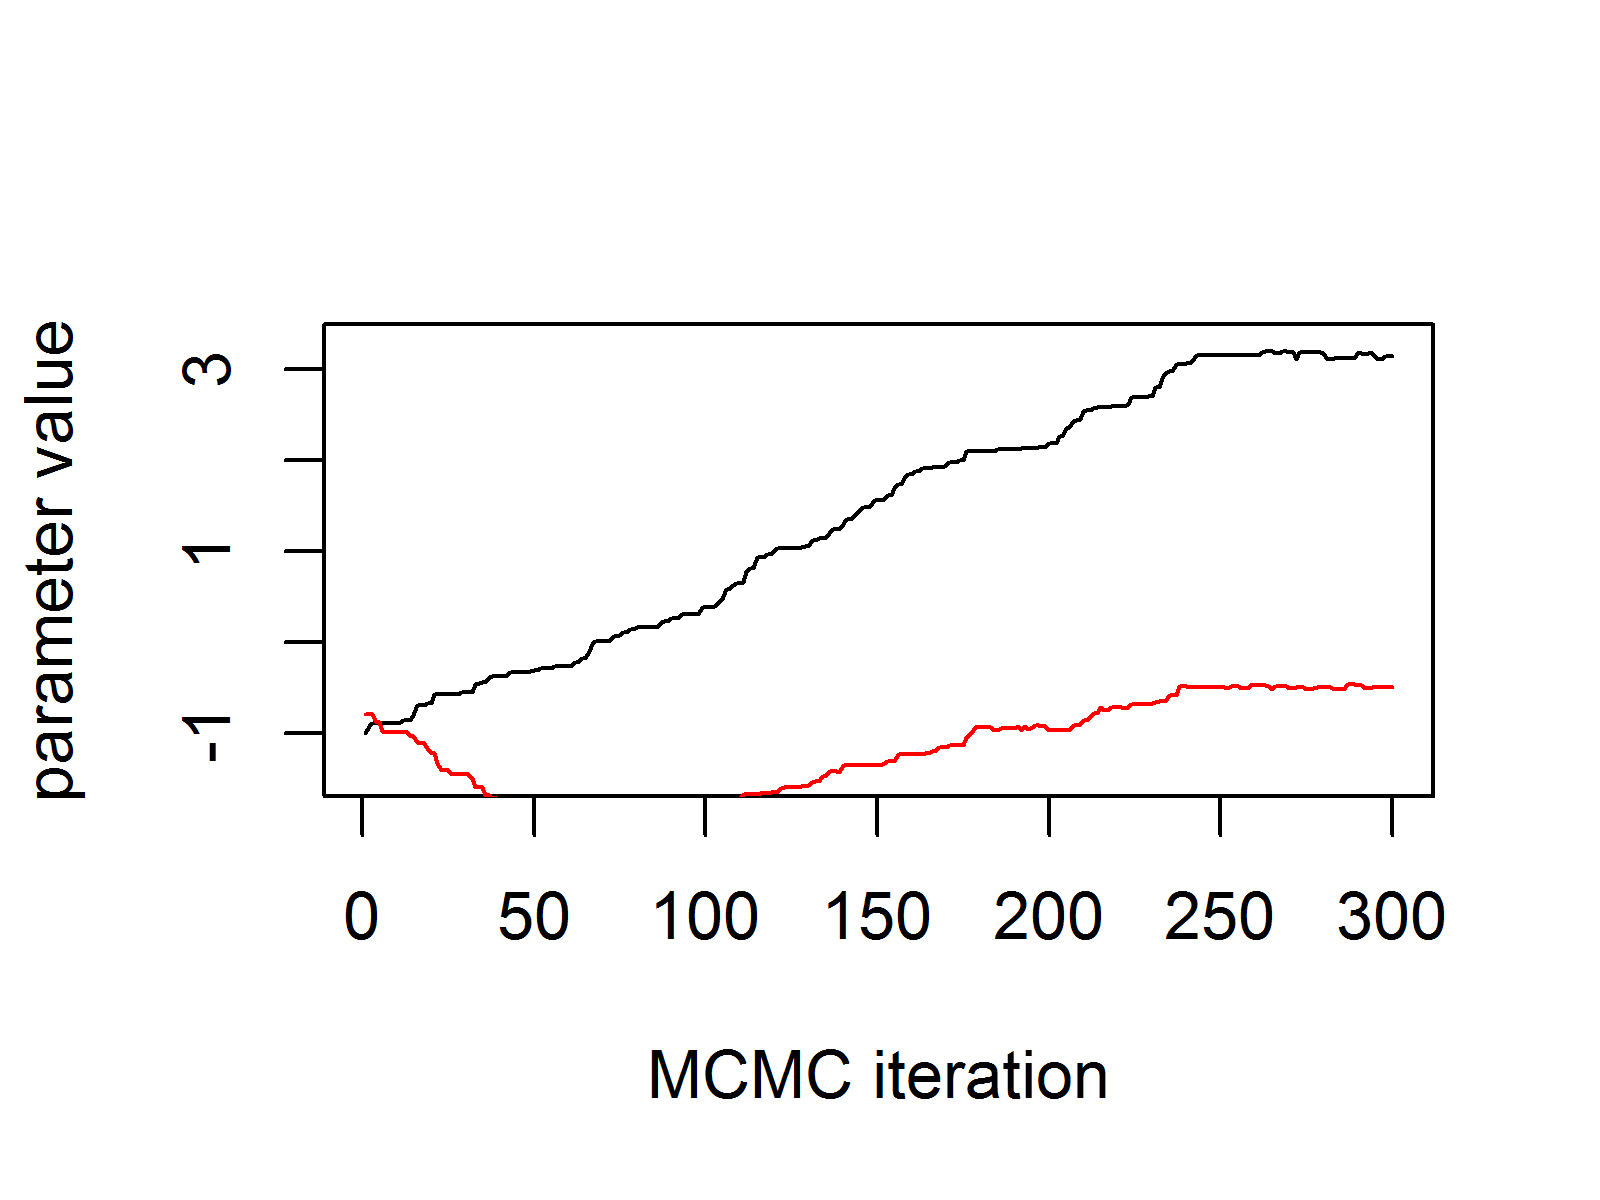
\includegraphics[height=3in,width=4in]{Ch2/figs/poissonmcmc2}
\end{center}
\caption{First 300 MCMC iterations for the Poisson GLM model parameters $\beta_0$ (black) and $\beta_1$ (red) using
a Metropolis-Hastings tuning parameter of
 $\delta = 0.05$.}
\label{glms.fig.poissonmcmc2}
\end{figure}

\begin{figure}
\begin{center}
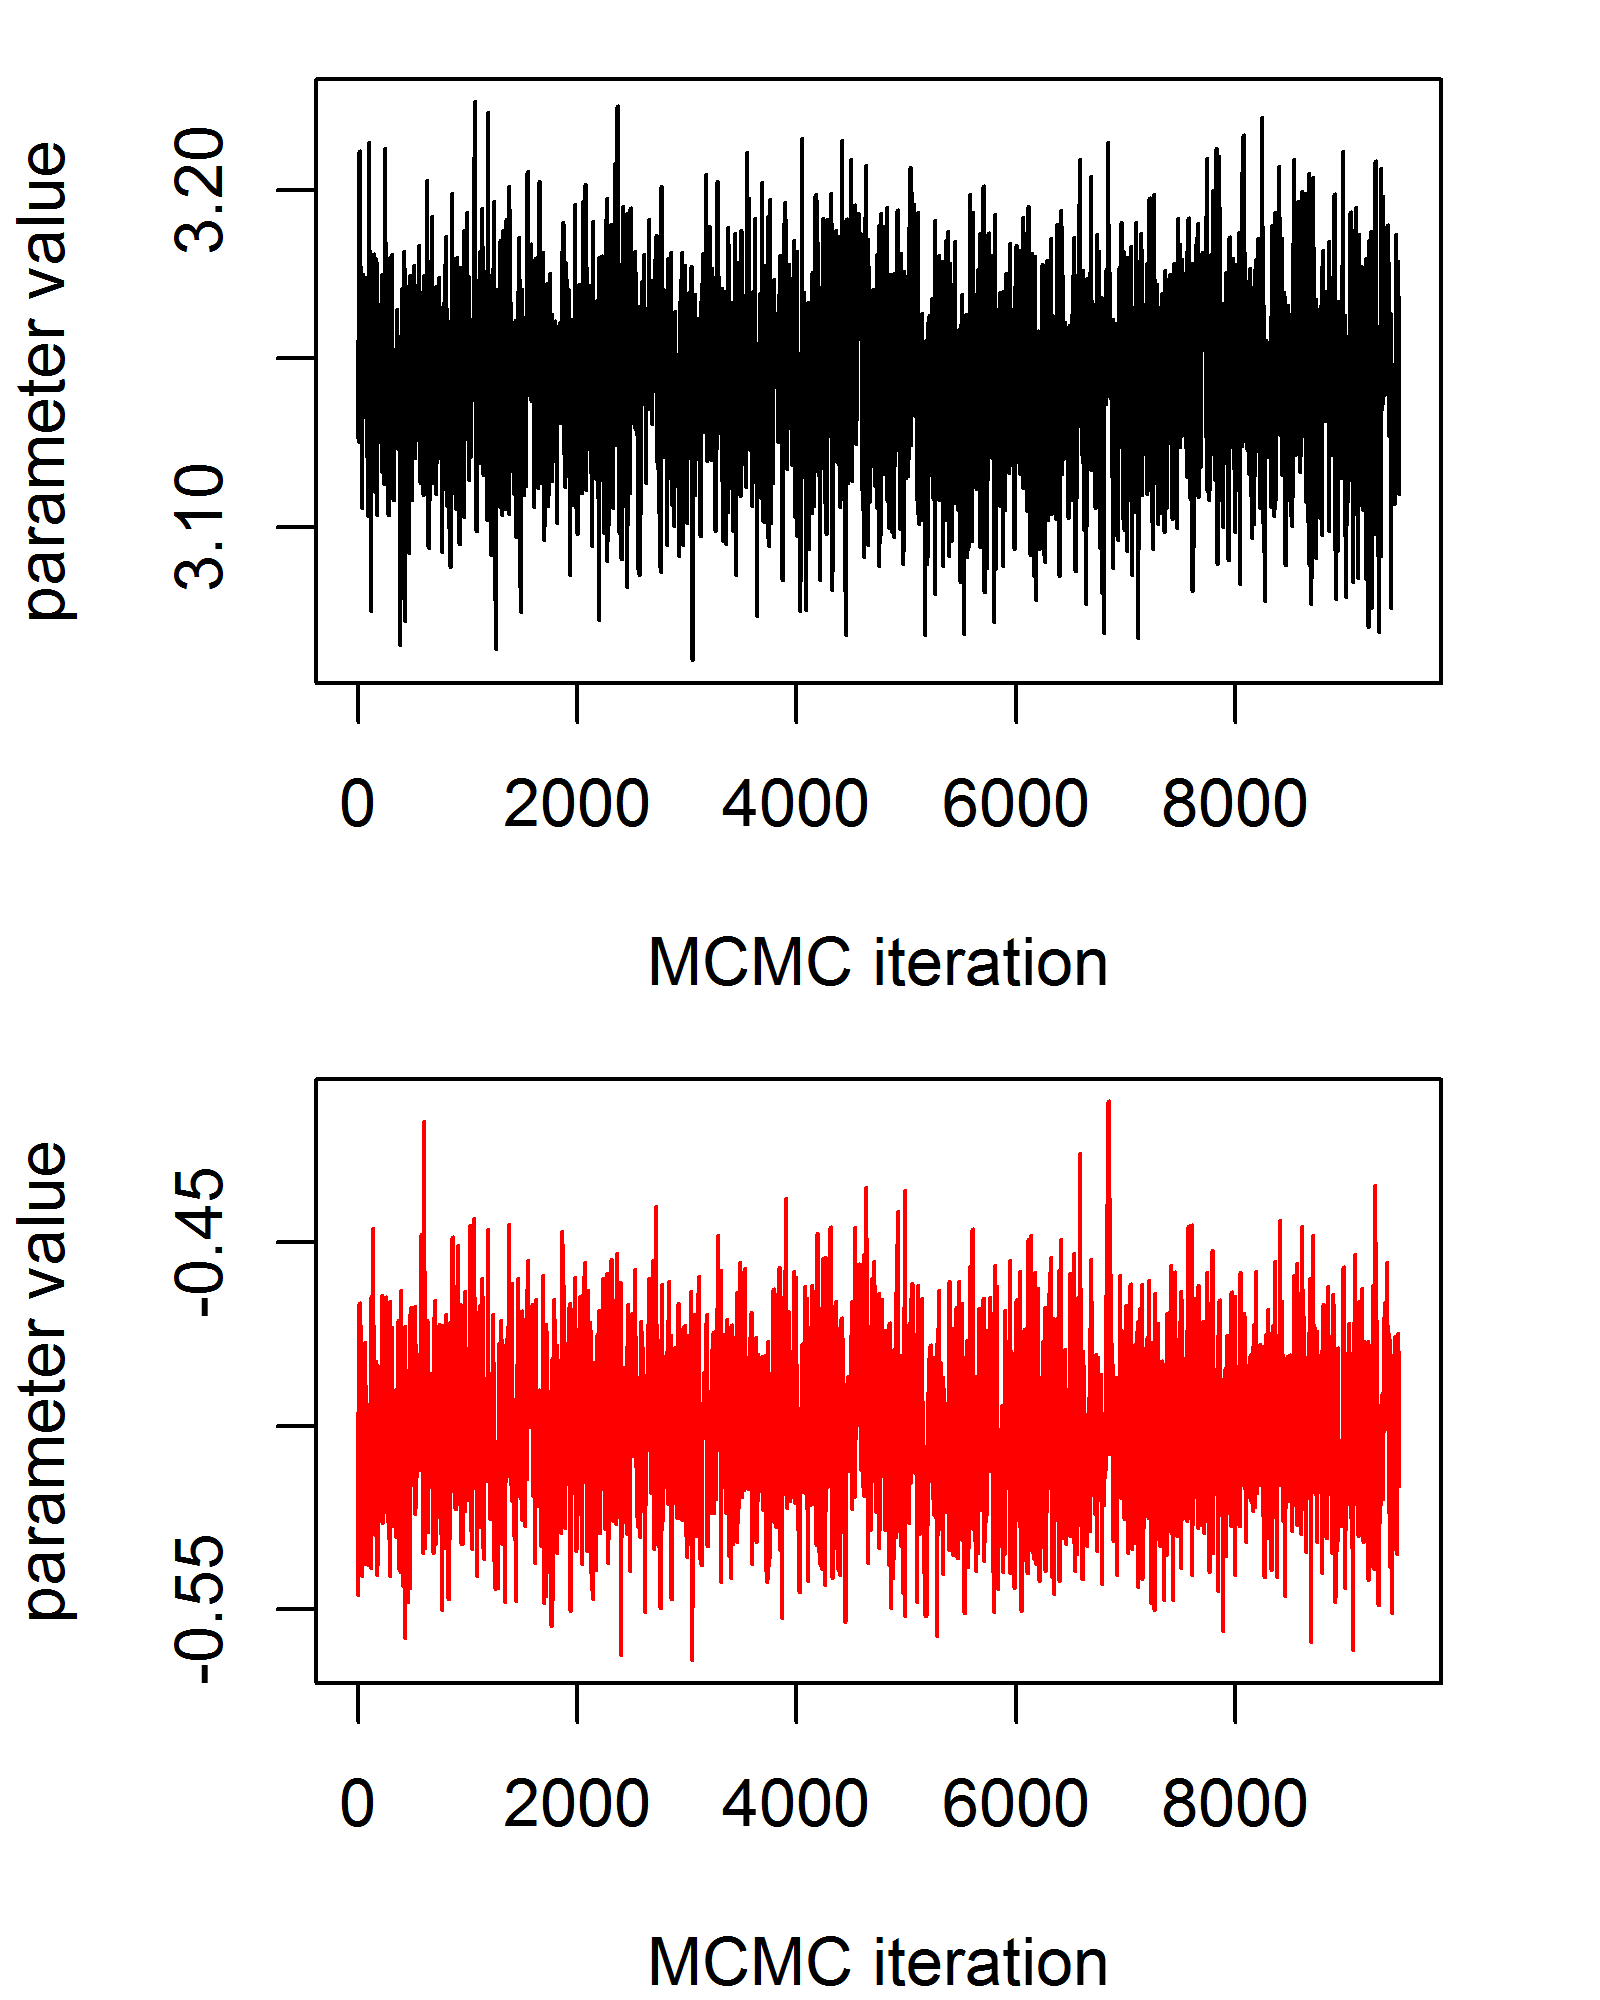
\includegraphics[height=4in,width=5in]{Ch2/figs/poissonmcmc3}
\end{center}
\caption{Nice grassy plots of 10,000 MCMC iterations for the Poisson GLM model parameters $\beta_0$ (black) and $\beta_1$ (red) using
a Metropolis-Hastings tuning parameter of
 $\delta = 0.05$.}
\label{glms.fig.grassy}
\end{figure}

Note that we used a specific set of starting values for these
simulations. It should be clear that starting values closer to the
mass of the posterior distribution might cause burn-in to occur
faster. As an exercise, evaluate that.  
Further, for the diffuse normal prior distributions
here we could leave the prior contribution out of the full conditional
evaluation since it is locally constant, i.e., constant in the vicinity of
the posterior mass, and thus has no practical effect. Removing the
prior contribution from the MH acceptance probability is equivalent to
saying that the parameters have an improper uniform prior, i.e.,
$\beta_0 \sim \mbox{const}$, which is commonly used for mean parameters
in practice.
Note also that we have
used a different prior than in our {\bf WinBUGS} model specification
given previously. As an
exercise, evaluate whether this seems to affect the result.

\section{Poisson GLM with Random Effects}

What we will be doing in most of this book is dealing with random
effects in GLM-like models - similar to what
are usually referred to as generalized
linear mixed models (GLMMs). We provide a brief introduction by way of
example, extending our Poisson regression model to include a random effect.


{\bf The Log-Normal mixture:} The classical situation involves a GLM
with a normally distributed random effect that is additive on the
linear predictor. For the Poisson case, we have:
\[
 	log(\lambda_{i}) = \beta_0  + \beta_1 x_{i} + \eta_{i}
\]
where $\eta_{i} \sim \mbox{Normal}(0,\sigma^{2})$.  A natural
alternative is to have multiplicative gamma-distributed noise,
$exp(\eta_{i}) \sim \mbox{Gamma}(a,b)$ which would correspond to a
negative binomial kind of over-dispersion, implying a different
mean/variance relationship to the log-normal mixture (the interested
reader should work that out).  Choosing between such possibilities is
not a topic we will get into here because it doesn't seem possible to
provide general guidance on it.  
% For this model we carried-out a
% goodness-of-fit evaluation using the Bayesian p-value based on a
% Pearson residual statistic. See also \citep[][ch. 18]{kery:2010} for
% an example involving a binomial mixed model\footnote{Kery has noticed
%   that such tests probably have 0 power. Should use the marginal
%   frequency of the data}. 
 Anyhow, it is really amazingly simple to
express this model in {\bf WinBUGS} and have {\bf WinBUGS} draw
samples from the posterior distribution using the following code for
the BBS dove counts: 
{\small
\begin{verbatim}
data(bbsdata)
locs<-bbsdata$counts[,2:3]
habitat<-bbsdata$counts[,4]
y<-bbsdata$counts[,29]     # grab year 1990
M<-length(y)

set.seed(2013)

cat("
model {
  for (i in 1:M){
     y[i]~dpois(lam[i])
     log(lam[i])<- beta0+ beta1*habitat[i] + eta[i]
     frog[i]<-beta1*habitat[i] + eta[i]
     eta[i] ~ dnorm(0,tau)
   }

 beta0~dunif(-5,5)
 beta1~dunif(-5,5)
 sigma~dunif(0,10)
 tau<-1/(sigma*sigma)
}

",file="model.txt")
data <- list ( "y","M","habitat")
inits <- function()
  list ( beta0=rnorm(1),beta1=rnorm(1),sigma=runif(1,0,4))
parameters <- c("beta0","beta1","sigma","tau")
library("R2WinBUGS")

out<-bugs (data, inits, parameters, "model.txt", n.thin=2,n.chains=2,
 n.burnin=1000,n.iter=5000,debug=TRUE)
\end{verbatim}
}

This produces the posterior summary statistics given in table \ref{glms.tab.bbspoisreg}. 

\begin{table}
\caption{Inference for Poisson GLM with habitat effect for mourning dove counts across BBS routes in PA, 1990, fit using WinBUGS,
 2 chains, each with 5000 iterations (first 1000 discarded), n.thin = 2
 n.sims = 4000 iterations saved.}
   \scriptsize
  \begin{tabular}{lccccccccc}
    \hline
        \hline
 Parameter &    mean   & sd   &  2.5\%    &  25\%  &    50\%   &   75\%  &  97.5\% & Rhat & n.eff \\
     \hline
beta0   &   2.98 & 0.08 &  2.82 &  2.93  & 2.98 &  3.03 &  3.12 & 1.00 & 1400 \\
beta1   &  -0.53 & 0.07 & -0.68 & -0.58 & -0.53 & -0.49 & -0.38 & 1.01 &  350 \\
sigma   &   0.60 & 0.06 &  0.49 &  0.56 &  0.59 &  0.64 &  0.73 & 1.00 & 2000 \\
tau     &   2.88 & 0.57 &  1.88 &  2.47 &  2.86 &  3.24 &  4.12 & 1.00 & 2000 \\
deviance & 445.94 & 12.18 & 424.00 & 437.40 & 445.20 & 453.90 & 471.50 & 1.00 & 4000 \\
    \hline
  \end{tabular}
  \label{glms.tab.bbspoisreg}
\vspace{0.5cm}
\end{table}


% {\small
% \begin{verbatim}
% print(out,digits=2)
% Inference for Bugs model at "model.txt", fit using WinBUGS,
%  2 chains, each with 5000 iterations (first 1000 discarded), n.thin = 2
%  n.sims = 4000 iterations saved
%            mean    sd   2.5%    25%    50%    75%  97.5% Rhat n.eff
% beta0      2.98  0.08   2.82   2.93   2.98   3.03   3.12 1.00  1400
% beta1     -0.53  0.07  -0.68  -0.58  -0.53  -0.49  -0.38 1.01   350
% sigma      0.60  0.06   0.49   0.56   0.59   0.64   0.73 1.00  2000
% tau        2.88  0.57   1.88   2.47   2.86   3.24   4.12 1.00  2000
% deviance 445.94 12.18 424.00 437.40 445.20 453.90 471.50 1.00  4000

% [... some output deleted ...]
% \end{verbatim}
}
% The Bayesian p-value for this model is
% \begin{verbatim}
% > mean(out$sims.list$fit>out$sims.list$fitnew)
% [1] 0.4815
% \end{verbatim}
% indicating a pretty good fit. Given the site-level random effect, it
% would be surprising for this model to not fit! 
One thing we notice is
that the posterior standard deviations of the regression parameters
are much higher, a result of the excess variation. We would also
notice much less precise predictions of hypothetical new
observations.




\section{Binomial GLMs}

Another extremely important class of models in ecology are
binomial models. We use binomial models for count data whenever the
observations are counts or frequencies and it is natural to condition
on a ``sample size'', say $K$, the maximum frequency possible in a sample.
 The random variable, $y \le K$, is then the
frequency of occurrences out of $K$ ``trials''. The parameter of the binomial
models is $p$, often called ``success probability'' which is related
to the expected value of $y$ by $E(y) = pK$. Usually we are interested
in modeling covariates that affect the parameter $p$, and such models
are called binomial GLMs , binomial
regression models or logistic regression, although logistic regression
 really only applies when the logistic link is used to model
the relationship between $p$ and covariates (see below).

One of the most typical binomial GLMs occurs when the sample size
equals 1 and the outcome, $y$, is ``presence'' ($y=1$) or ``absence''
($y=0$) of a species. This is a classical ``species distribution''
modeling situation. A special situation occurs when presence/absence
is observed with error \citep{mackenzie_etal:2002,tyre_etal:2003}.
In that case, $K>1$ samples
are usually needed for effective estimation of model parameters.

 In standard binomial regression problems the sample size
is fixed by design but interesting models also arise when the sample
size is itself a random variable. These are the $N$-mixture models
\citep{royle:2004, kery_etal:2005, royle_dorazio:2008, kery:2010}
and related models (in this case, $N$ being the sample size,
which we labeled $K$ above)\footnote{Some of the jargon is actually a little
bit confusing here
because the binomial index is customarily referred to as ``sample size''
but in the context of $N$-mixture models $N$ is actually the
``population size''}.
Another
situation in which the binomial sample size is ``fixed'' is closed
population capture-recapture models in which a population of
individuals is sampled $K$ times.  The number of times each individual
is encountered is a binomial outcome with parameter - encounter
probability -- $p$, based on a sample of size $K$.  In addition, the
total number of unique individuals observed, $n$, is also a binomial
random variable based on population size $N$.  We consider such
models in Chapt. \ref{chapt.closed}.


\subsection{Binomial regression}

In binomial models, covariates are modeled on a suitable
transformation (the link function) of the binomial success
probability, $p$.  Let $x_{i}$ denote some measured covariate for
sample unit $i$ and let $p_{i}$ be the success probability for unit $i$.
The standard choice is the logit link function (\ref{glms.sec.glmms}) but there are many other possible link functions. However, ecologists seem
to adopt the logit link function without question in most
applications\footnote{a notable exception is distance sampling, which
  is all about choosing among link functions}.  We sometimes use the
``complementary log-log'' (= ``cloglog'') link function in ecological
applications because it arises naturally in many situations
\citep[][p. 150]{royle_dorazio:2008}. For example, consider the
``probability of observing a count greater than 0'' under a Poisson
model: $\Pr(y>0) = 1-exp(- \lambda)$. In that case,
\[
cloglog(p) =log(- log(1-p)) = log(\lambda)
\]
So that if you have covariates in your linear predictor for $E(y)$
under a Poisson model then they are linear on the complementary
log-log link of $p$.
In models of species occurrence it seems natural to view occupancy as
being derived from local abundance $N$
\citep{royle_nichols:2003,royle_dorazio:2006,dorazio:2007}.
Therefore,
models of local abundance in which $N \sim \mbox{Poisson}(A \lambda)$
for a habitat patch of area $A$ implies a model for occupancy $\psi$
of the form
\[
 cloglog(\psi) = log(A) + log(\lambda).
\]
We will use the cloglog link in some analyses of
SCR models in Chapt. \ref{chapt.scr0} and elsewhere.


\subsection{ Example: Waterfowl Banding Data}

It would be easy to consider a standard ``distribution modeling''
application where $K=1$ and the outcome is occurrence ($y=1$) or not
($y=0$) of some species. Such examples abound in books (e.g.,
\citet[][ch. 3]{royle_dorazio:2008}; \citet[][ch. 21]{kery:2010};
\citet[][ch. 13]{kery_schaub:2011}) and in the literature.
Instead, we will
consider an example involving band returns of waterfowl in the upper great plains including some canadian provinces, which were
analyzed by \citet{royle_dubovsky:2001}\footnote{I hate this example.
  Anyone got a better one thats not distribution modeling?}.

For these data, $y_{it}$ is the number of mallard ({\it Anas platyrhynchos}) bands recovered out
of $B_{it}$ birds banded at some location ${\bf s}_{i}$ in year $t$. In this case $B_{it}$ is
fixed. Thinking about recovery rate as being proportional to harvest
rate, we use these data to explore geographic gradients in recovery rate
resulting from variability in harvest pressure experienced by
populations depending on their migration ecology. As such, we fit a
basic binomial GLM with a linear response to geographic coordinates
(including an interaction term). 
% The data ({\tt mallarddata}) are provided with the {\bf
%   R} package \mbox{\tt scrbook}. XXX MAYBE ADD LATER XXXX
Here we
 provide the part of the script for creating the model and fitting the
 model in
{\bf WinBUGS} using the \mbox{\tt bugs} function.
There are few structural differences between this model and the
Poisson GLM fitted previously. The main things are due to the data
structure (we have a matrix here instead of a vector) and otherwise we
change the main distributional assumption to binomial (specified with
\mbox{\tt dbin}) and then use the \mbox{\tt logit} function to relate
the parameter $p_{it}$ to the covariates.  

{\flushleft \bf Dummy variables in BUGS: } 
In Chapt. \ref{CH2} we introduced the concept of categorical variables and how to display them in model formulas in the form of ``dummy variables''. In the mallard example, we model the band recovery probability $p$ not only as a linear function (on the logit scale) of geographic location, but also allow for variation in $p$ with year, $t$; $t=1,2,...T$. In this particular example there are T=5 years of data and if we wanted to describe the full mallard model with a formula adopting the dummy variable format, it would look like this:
\[
y_{it} \sim Binomial(p_{it}, B_{it}}
logit(p_{it}) = \beta_0 + \beta_1 Sv2_t + \beta_2 Sv3_t + \beta_3 Sv4_t + \beta_4 Sv5_t + \beta_5 lat_i + \beta_6 lon_i + \beta_7 lat_i lon_i
\]
Here, $Sv2$ to $Sv5$ are the dummy variable vectors of length $T$ that take on the value of 1 when $t$ corresponds to the respective year and 0 otherwise. For example, Sv2 = (0,1,0,0,0). $\beta_0$ is the common intercept term and correspond to $t=1$; $\beta_1$ - $\beta_4$ describe the difference in $p$ for each $t$ \emph{relative to} $t=1$.

There is a more concise way of implementing such a model with a categorical covariate in {\bf BUGS}, namely, by using indexing instead of dummy variables (actually, in some cases a model may mix or converge better depending on whether you choose a dummy variable or an indexing description of it, although they are structurally equivalent \citep{kery:2010}). Essentially, instead of estimating the difference in $p$ relative to survey 1, we  estimate a separate intercept term for each survey, so that we have 5 different $beta_0$ indexed by $t$. This reduces the linear predictor to:
\[
logit(p_{it}) = \beta_{0t} +  \beta_5 lat_i + \beta_6 lon_i + \beta_7 lat_i lon_i
\]
We show you how to implement that in {\BUGS} for this mallard example. Here is the script:

{\small
\begin{verbatim}
load("mallarddata")  # not sure how this will look

sink("model.txt")
cat("
model {
 for(t in 1:5){
    for (i in 1:nobs){
       y[i,t] ~ dbin(p[i,t], B[i,t])
       logit(p[i,t]) <- beta0[t] + beta1*X[i,1] + beta2*X[i,2] + beta3*X[i,1]*X[i,2]
     }
}
	beta1~dnorm(0,.001)
	beta2~dnorm(0,.001)
	beta3~dnorm(0,.001)
	for(t in 1:5){
 	beta0[t] ~ dnorm(0,.001)
 }
}
",fill=TRUE)
sink()

data  <- list(B=mallard.bandings, y=mallard.recoveries,
             nobs=nrow(banding.locs),X=banding.locs)
inits <- function(){
      list(beta0=rnorm(5),beta1=0,beta2=0,beta3=0) }
parms <- list('beta0','beta1','beta2','beta3')
out   <- bugs(data,inits, parms,"model.txt",n.chains=3,
 	n.iter=2000,n.burnin=1000, n.thin=2,debug=TRUE)
\end{verbatim}
}

\begin{table}
\caption{Inference for binomial GLM with effects of year(alpha0) and geographic loation (alpha1 - alpha3) on mallard band recovery probabilities, fit using WinBUGS, 3 chains, each with 2000 iterations (first 1000 discarded), n.thin = 2
 n.sims = 1500 iterations saved.}
   \scriptsize
  \begin{tabular}{lccccccccc}
    \hline
        \hline
 Parameter &    mean   & sd   &  2.5\%    &  25\%  &    50\%   &   75\%  &  97.5\% & Rhat & n.eff \\
     \hline
alpha0[1]  & -2.346 0.036 &  -2.417 &  -2.370 &  -2.346 &  -2.323 &  -2.277 & 1.001 & 1500 \\
alpha0[2] &  -2.356 0.032 &  -2.420 &  -2.379 &  -2.356 &  -2.335 &  -2.292 & 1.001 & 1500 \\
alpha0[3] &  -2.220 0.035 &  -2.291 &  -2.244 &  -2.219 &  -2.197 &  -2.153 & 1.001 & 1500 \\
alpha0[4] &  -2.144 0.039 &  -2.225 &  -2.169 &  -2.143 &  -2.116 &  -2.068 & 1.000 & 1500 \\
alpha0[5] &  -1.925 0.034 &  -1.990 &  -1.949 &  -1.924 &  -1.901 &  -1.856 & 1.004 & 570 \\
alpha1    &  -0.023 0.003 &  -0.028 &  -0.025 &  -0.023 &  -0.022 &  -0.018 & 1.001 & 1500 \\
alpha2    &   0.020 0.006 &   0.009 &   0.016 &   0.020 &   0.024 &   0.031 & 1.001 & 1500 \\
alpha3    &   0.000 0.001 &  -0.002 &  -0.001 &   0.000 &   0.000 &   0.002 & 1.001 & 1500 \\
deviance & 1716.001 4.091 & 1710.000 & 1713.000 & 1715.000 & 1718.000 & 1726.000 & 1.001 & 1500 \\
    \hline
  \end{tabular}
  \label{glms.tab.mallard}
\vspace{0.5cm}
\end{table}

% {\small
% \begin{verbatim}
% > print(out,digits=3)
% Inference for Bugs model at "model.txt", fit using WinBUGS,
%  3 chains, each with 2000 iterations (first 1000 discarded), n.thin = 2
%  n.sims = 1500 iterations saved
%               mean    sd     2.5%      25%      50%      75%    97.5%  Rhat n.eff
% alpha0[1]   -2.346 0.036   -2.417   -2.370   -2.346   -2.323   -2.277 1.001  1500
% alpha0[2]   -2.356 0.032   -2.420   -2.379   -2.356   -2.335   -2.292 1.001  1500
% alpha0[3]   -2.220 0.035   -2.291   -2.244   -2.219   -2.197   -2.153 1.001  1500
% alpha0[4]   -2.144 0.039   -2.225   -2.169   -2.143   -2.116   -2.068 1.000  1500
% alpha0[5]   -1.925 0.034   -1.990   -1.949   -1.924   -1.901   -1.856 1.004   570
% alpha1      -0.023 0.003   -0.028   -0.025   -0.023   -0.022   -0.018 1.001  1500
% alpha2       0.020 0.006    0.009    0.016    0.020    0.024    0.031 1.001  1500
% alpha3       0.000 0.001   -0.002   -0.001    0.000    0.000    0.002 1.001  1500
% deviance  1716.001 4.091 1710.000 1713.000 1715.000 1718.000 1726.000 1.001  1500

% [... some output deleted ...]
% \end{verbatim}
% }


Look at the posterior summaries of model parameters in Table \ref{glms.tab.mallard}. The basic result suggests a negative east-west gradient and a positive
south to north gradient of abnd recovery probabilities, but no interaction. A map of the response
surface is shown in Fig. \ref{glms.fig.bandrecovery}.
%  We did an additional MCMC run where we saved the binomial
% parameter $p$ and computed the Bayesian p-value (double use of ``p''
% here is confusing, but I guess that happens sometimes!)
% using a fit statistic based on the Freeman-Tukey
% statistic (see Sec. \ref{glms.sec.gof}
% above). The result indicates that the
% linear response surface model does not provide an adequate fit of the
% data. The reader should contemplate whether this invalidates the basic
% interpretation of the result.


\begin{figure}
\begin{center}
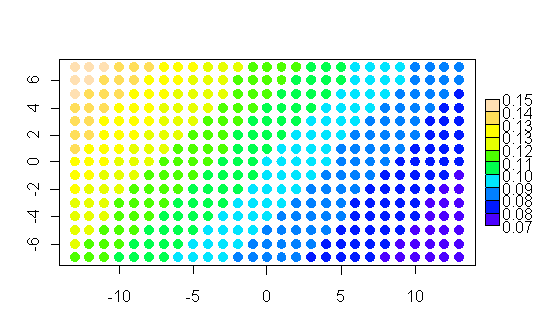
\includegraphics[height=2.75in]{Ch2/figs/responsesurface}
\end{center}
\caption{Predicted recovery rates of mallard bands across the upper great plains. Note the negative east-west gradient.}
\label{glms.fig.bandrecovery}
\end{figure}

\section{ Summary and Outlook}

GLMs and GLMMs are the most useful statistical methods in all of
ecology. The principles and procedures underlying these methods are
relevant to nearly all modeling and analysis problems in every branch
of ecology. Moreover, understanding how to analyze these models is
crucial in a large number of diverse problems. If you understand and
can conduct classical likelihood and Bayesian analysis of Poisson and
binomial GLM(M)s, then you will be successful analyzing and
understanding more complex classes of models that arise. We will see
shortly that spatial capture-recapture models are a type of GLMM
and thus having a basic
understanding of the conceptual origins and formulation of GLM(M)s and
their analysis is extremely useful.

We note that GLM(M)s are routinely
analyzed by likelihood methods but we have focused on Bayesian
analysis here in order to develop the tools that are less familiar to
most ecologists, and that we will apply in much of the remainder of the book.  In particular, Bayesian analysis of models with random
effects is relatively straightforward because the models
are easy to analyze conditional on the random effect, using methods of
MCMC.  Thus, we will often analyze SCR models in later chapters by
MCMC, explicitly adopting a Bayesian inference framework.
In that regard, the various {\bf BUGS} engines ({\bf WinBUGS}, {\bf
  OpenBUGS}, {\bf JAGS}; see also \ref{chapt.app1}) are enormously useful because they
provide an accessible platform for
carrying out  analyses by MCMC by just
describing the model, and not having to worry about how to actually
build MCMC algorithms.  That said, the {\bf BUGS} language is more important
than just to the extent that it enables one to do MCMC - it is useful
as a modeling tool because it fosters understanding, in the sense that
it forces you to become intimate with your model. You have to write
down all of the probability assumptions, the relationships between
observations and latent variables and parameters. This is really a
great learning paradigm that you can grow with.

While we have emphasized Bayesian analysis in this chapter, and make
primary use of it through the book, we
we will provide an introduction to likelihood analysis in Chapt.
\ref{chapt.mle} and use those  methods also from time to time.
 Before getting to that, however, it will be useful to
talk about more basic, conventional closed population
capture-recapture models and these are the topic of the next chapter.


\chapter{
 Closed Population Models
}
\markboth{Chapter 3}{}
\label{chapt.closed}

\vspace{.3in}

Having covered some basics of standard % "standard" is a little vague
models and their implementation in \textbf{BUGS} software,
in this chapter we will consider ordinary capture-recapture (CR)
models for estimating population size in closed populations. A closed
population is one whose abundance $N$ does not change during the
study. Two forms of closure are often discussed: demographic closure,
meaning that no births or deaths occur, and geographic closure, which
means that no individuals do not move onto or off of the study
area. Few populations are actually closed except during very short
time intervals, but closed population CR models serve as the basis for
the development of the rest of the models presented in this book,
including the models for open populations discussed in
Chapt.\ref{chapt.open}.

We will
see that classical closed population CR models are closely related to binomial (or logistic)
regression-type models. In fact, when $N$ is known, they are precisely
logistic regression models.  We consider some important extensions of ordinary closed
population models that accommodate various types of ``individual
effects'' --- either in the form of explicit, observed %and measured
covariates (sex, age,
body mass) or unstructured ``heterogeneity'' in the form of an
individual random effect, which represent effects of unobserved or
unmeasured covariates. In general, these models are variations of
generalized linear or generalized linear mixed models (GLMs and GLMMs, respectively).
Because of the paramount importance of this concept, we focus mainly
on fairly simple models in which the observations are individual
encounter frequencies, $y_{i}$ = the number of encounters of
individual $i$ out of $K$ replicate samples of the population which,
for the models we consider here, is the outcome of a binomial random
variable.  Along the way, we consider the spatial context of
capture-recapture data %and models
and demonstrate that density cannot
be formally estimated when spatial information is ignored. We also
review some of the informal methods of estimating density using CR
methods, and consider some of their limitations.  We will be exposed
to our first primitive spatial capture-recapture models which arise as
relatively minor variations of so-called ``individual covariate
models'' (of the \citet{huggins:1989} and \citet{alho:1990}
variety). In a sense, the point of this chapter is to establish the %that
linkage  between non-spatial and spatial capture-recapture models
 in a direct and concise manner beginning with the most basic
 capture-recapture model colloquially referred to as ``model $M_0$''
 \citep{otis_etal:1978} in which encounter probability is strictly
 constant in all respects (across individuals, and replicates), and
 extensions of that model to include individual
heterogeneity and individual covariates. A special type of
individual covariate models is distance sampling, which could be
thought of as the most primitive spatial capture-recapture model. In
later chapters we further develop and extend ideas introduced in this
chapter.

We emphasize Bayesian analysis of capture-recapture models and we
accomplish this using a method related to classical ``data
augmentation'' from the statistics literature
\citep[e.g.,][]{tanner_wong:1987}.  This is a general concept in
statistics but, in the context of capture-recapture models where $N$
is unknown, it has a consistent implementation across classes of
capture-recapture models and one that is really convenient from the
standpoint of doing MCMC \citep{royle_etal:2007,royle_dorazio:2011}. We use data
augmentation throughout this book and thus emphasize its conceptual
and technical origins and demonstrate applications to closed
population models.  We refer the reader to
\citet[][ch. 6]{kery_schaub:2011} for an accessible and complementary
development of Bayesian analysis of ordinary, i.e., nonspatial closed population models.


\section{The Simplest Closed Population Model: Model $M_0$}

To start looking at the simplest capture-recapture model, let's suppose
there exists a population of $N$ individuals which we
subject to repeated sampling, say over $K$ ``occasions'', such as trap nights, where individuals
are captured, marked, and subsequently recaptured.  We suppose that
individual encounter histories are obtained, and these are of the form
of a sequence of 0's and 1's indicating capture $(y=1)$ or not $(y=0)$
during any sampling occasion% XXX (``sample'') I prefer occasion since a
                            % sample could be spatial
.  As an example, suppose
$K=5$ sampling occasions, then an individual captured during occasion % sample
2 and 3 but not otherwise would have an encounter history of the form
${\bf y}=(0,1,1,0,0)$. Thus, the observation ${\bf y}_{i}$ for each
individual $(i=1,2,\hdots,N)$ is a vector having elements denoted by $y_{ik}$ for
$k=1,2,\hdots,K$. Usually this is organized as a row of a matrix with
elements $y_{ik}$, see Table \ref{closed.tab.3.1}. Except where noted
explicitly, we suppose that observations are independent within
individuals and among individuals.  Formally, this allows us to say
that $y_{ik}$ are $iid$ % XXX somewhere we should write this out. And we
                        % need to be consistent--sometimes we use i.i.d.
Bernoulli random variables and we may write $y_{ik}
\sim \mbox{Bern}(p)$.  Consequently, for this very simple model in
which $p$ is constant (i.e., there are no individual or temporal
covariates that affect $p$) the original binary detection variables
can be aggregated into total encounter frequencies for each individual
(total number of captures), $y_{i} = \sum_{k} y_{ik}$, and the
observation model changes from a Bernoulli distribution to a
binomial distribution based on a sample of size $K$. That is
\[
y_{i}  = \sum_{k} y_{ik} \sim \mbox{Bin}(p,K)
\]
for every individual in the population $i=1,2,\ldots,N$, where $N$ is
the number of individuals in the population (i.e., population size).

We emphasize the central importance of the basic Bernoulli encounter model
-- an individual is either encountered in a sample, or not --
 which forms
the cornerstone of almost all of classical
capture-recapture models, including many spatial capture-recapture
models discussed in this book.

Evidently, the basic capture-recapture model is a
simplistic version of a logistic-regression model with only an
intercept term ($\mbox{logit}(p) = \mbox{constant}$).  To say that all
capture-recapture models are just logistic regressions is only
slightly inaccurate. In fact, we are proceeding here as if we knew $N$.
In practice we don't, of course, and
%that is kind of the point of capture-recapture models as
estimating
$N$ is actually the central objective.
But, by proceeding as if $N$ were known,
we can specify a simple model and then deal with the
fact that $N$ is unknown using standard methods that you are already
familiar with (i.e., GLMs - see Chapt. \ref{chapt.glms}).
\begin{table}
\centering
\caption{A toy capture-recapture data set with $n=6$ observed
  individuals and $K=5$ sample occasions. Under a model with constant encounter
  probability, the binary detection history data can be summarized in the detection frequency (the total number of detections, $y_i$), which is shown in the right-most column.
}
\begin{tabular}{r|ccccc|c}
\hline
&  \multicolumn{5}{c}{Sample occasion} &  \\ \hline
 indiv $i$ &  1 & 2 & 3 & 4 & 5 & $y_{i}$ \\ \hline
  1 &     1 & 0 & 0 & 1 & 0  & 2   \\
  2 &     0 & 1 & 0 & 0 & 1  & 2   \\
  3 &     1 & 0 & 0 & 1 & 0  & 2   \\
  4 &     1 & 0 & 1 & 0 & 1  & 3   \\
  5 &     0 & 1 & 0 & 0 & 0  & 1   \\
  $n=6$ & 1 & 0 & 0 & 0 & 0  & 1   \\ \hline
\end{tabular}
\label{closed.tab.3.1}
\end{table}


\begin{comment}
While the Bernoulli observation model is the fundamental model of the
individual encounter process in all of capture-recapture, when we sum
those up we have a binomial observation model and, when $N$ is
unobserved, we have something of a zero-truncated binomial
model.......... XXXX
\end{comment}

\begin{comment} xxxxxx  $Perhaps explain how the very basic observation model in all
of capture-recapture is Bernoulli: a guy is either seen or
not. However, often we analyse a summary of this, for instance in the
form of the sum of N Bernoulli trials, leading to a Binomial, or in
the form of a Multinomial, which really also is a form of an
incomplete summary or something$ xxxxxx \end{comment}


Assuming individuals in the population are observed independently, the
joint probability distribution of the observations is the product of
$N$ binomials
% This is very condensed, so I tried to break it up
%\begin{eqnarray}
%  \Pr(y_1, \ldots, y_N | p) &=& \prod_{i=1}^N  \mathrm{Bin}(y_i | K, p) \\
%   &=& \prod_{k=0}^K  \pi(k)^{n_k}
%\label{closed.eq.binNknown}
%\end{eqnarray}
\begin{equation}
  \Pr(y_1, \ldots, y_N | p) = \prod_{i=1}^N  \mathrm{Bin}(y_i | K, p).
  \label{closed.eq.binNknown}
\end{equation}
This expression can be simplified even further if we reformat the
observations as capture frequencies, which are the sufficient
statistics under this model. Specifically, let $n_k$ denote the number
of individuals captured $k$ times after $K$ survey occasions, $n_k = \sum_{i=1}^N
I(y_i = k)$ where $I$ is the indicator function evaluating to 1 if its
argument is true and 0 otherwise. For sake of illustration,
we converted the data from TableTable~\ref{closed.tab.3.1} to this
format (Table~\ref{closed.tab.3.1.nk}). An equivalent expression to
Eq.~\ref{closed.eq.binNknown} can now be written as
\begin{equation}
  \Pr(y_1, \ldots, y_N | p) = \prod_{k=0}^K  \pi(k)^{n_k}
  \label{closed.eq.multiNknown}
\end{equation}
where $\pi(k) = \mathrm{Bin}(k | K,p)$.
We emphasize that both expressions are conditional on $N$, in which
case we get to observe the $y_i=0$ observations and the resulting data
are just $iid$ binomial counts. Because this is a binomial regression
model of the variety described in Chapt. \ref{glms}, fitting this model using
a {\bf BUGS} engine poses no difficulty.


The essential problem in capture-recapture, however, is that $N$ is
{\it not} known because the number of uncaptured %/missing
individuals ($n_0$)
%(i.e., those in the zero cell that occur with probability $\pi_0$)
is unknown. % I added some text here, which is kind of clunky but this
            % section was moving too fast I think.
\begin{table}
\centering
\caption{Data from Table~\ref{closed.tab.3.1} formatted as capture
  frequencies. Since $N$ is unknown, the number of individuals not
  captured ($n_0$) is also unknown.}
\begin{tabular}{lcccccc}
\hline
& \multicolumn{6}{c}{$k$} \\
\cline{2-7}
 & 0  & 1 & 2 & 3 & 4 & 5 \\
\hline
Number of individuals captured $k$ times ($n_k$) & $N-6$ & 2 & 3 & 1 & 0 & 0 \\
\hline
\end{tabular}
\label{closed.tab.3.1.nk}
\end{table}
Consequently, the observed capture frequencies $n_k$ are no
longer independent because $n_0$ is a function of the other
frequencies (as well as $N$), $n_0 = N-\sum_{k=1}^K n_k$. Hence, their joint distribution is multinomial
(e.g., see \citet[][p. xyz]{illian_etal:2008}):
%\hl{Andy, I changed this from n_1, n_2 to n_0, n_1. Isn't that right?}
\begin{equation}
    n_0, n_1, \ldots, n_K \sim \mathrm{Multin}(N, \pi_0, \pi_1, \ldots, \pi_K)
\label{closed.eq.multinomial4m0}
\end{equation}
We give a general overview of the multinomial distribution in
sec. \ref{sec.modeling.distributions}. The multinomial distribution is
the standard model for discrete responses that can fall into a fixed
number ($K+1$ in this case) of possible categories. In the context of
capture-recapture, the multinomial posits a population of $N$
individuals with $K+1$ possible outcomes defined by the possible
encounter frequencies. These possible outcomes occur with
probabilities $\pi_{k}$, which we refer to as ``cell probabilities''
or in the specific context of capture-recapture, encounter history
probabilities.
%We denote the number of uncaptured/missing individuals
%by $n_0$, and the total number of distinct individuals encountered in
%the $K$ samples by $n = \sum_{k=1}^K n_k$.  Note that $n_{0}$ appears
%in the likelihood as a component of $N = n + n_{0}$.


To fit the model in which $N$ is {\it unknown}, we can regard $n_{0}$ as a
parameter and maximize the multinomial likelihood directly.
Direct likelihood analysis of the multinomial model is
straightforward, but that does not prove to be too useful in practice
because we seldom are concerned with models for the aggregated
encounter history frequencies, which entail that capture probabilities are the
same for all individuals. In many instances, including for
spatial capture-recapture (SCR) models, we require a formulation of
the model that can accommodate individual-level
covariates to account for
differences in detection among individuals which we
address subsequently in this chapter and also in Chapt. \ref{chapt.covariates}.



\begin{comment}
\subsection{The Spatial Context of Capture-Recapture}

XXX I WOULD CHANGE THE SECTION HEADING TO SOMETHING LIKE 'POPULATION CLOSURE AND THE SPATIAL
CONTEXT OF CAPTURE-RECAPTURE XXX

A common assumption made is that of population ``closure'' which is
really just a colloquial way of saying (in part) the Bernoulli
assumptions stated explicitly above. In the biological context,
closure means, strictly, no additions or subtractions from the
population during study. This is manifest by the statement that the
encounters are independent and identically distributed (iid) Bernoulli
trials.  In practice, closure is usually interpreted by the manner in
which potential violations of that assumption arise. In particular,
two important elements of the closure assumption are ``demographic''
and ``geographic'' closure. If an individual dies then subsequent
values of $y_{ik}$ are clearly no longer Bernoulli trials with the
same parameter $p$; since the probability of capturing that individual becomes 0. If there is no mortality or recruitment in the
population, then we say that demographic closure is
satisfied. Similarly, animals may emigrate or immigrate. If they do
not, then geographic closure is satisfied. Sometimes a distinction is
made between temporary and permanent emigration or immigration. That
is a relevant distinction in spatial capture-recapture models, because
SCR models explicitly accommodate ``temporary emigration'' of a
certain type, due to individuals moving about their home range.
In contrast, ordinary capture-recapture models cannot explicitly deal
with the fact that, unless we're sampling a fenced enclosure or an
island, individuals are bound to move ``off the trapping grid''
(whatever that means).  The
demographic closure assumption can also be relaxed using SCR models,
but we will save that discussion for Chapt. \ref{chapt.scr0}.

XXXX I FEEL LIKE THIS SECTION STILL NEEDS A SENTENCE THAT MAKES THE POINT - SPATIAL CONTEXT; POP CLOSURE AND SCR;
BUT I AM HAVING TROUBLE PUTTING THAT INTO A FEW WORDS RIGHT NOW XXXX

\end{comment}

\subsection{The Core Capture-Recapture Assumptions}

In addition to the assumption of population closure,
\citet{otis_etal:1978} list the following:
\begin{enumerate}
  \item animals do not lose their marks during the experiment,
  \item all marks are correctly noted and recorded at each trapping
    occasion, and
  \item each animal has a constant and equal probability of capture on
    each trapping occasion.
\end{enumerate}
The remainder of their classic work is dedicated to relaxing
assumption 3. While assumptions 1 and 2 are undoubtedly necessary for
inference from basic CR methods to be valid, and while they are
also assumed by most of the models we present in the following
chapters, we refrain from repeatedly making such statements. Our
opinion is that all model assumptions are apparent when a model is
clearly specified. For instance, if we write
\[
y_i \stackrel{iid}{\sim} \text{Bernoulli}(p) \quad \: \text{for} i=1,\ldots,N
\]
then there is not much more to say with respect to assumptions. For
example, if animals lost their marks, then clearly this statement would
not apply because we would not be able to know which individual we
encountered. Likewise for assumption 2.



Encounter events of the same individual are independent of one
another. Usually this is not, but we can build models that contain
covariates.
Of course spatial location is a sensible covariate for encounter
probability and the whole point of SCR models is to induce a certain
type of non-independence as a result of individual location relative
to traps.

Independence of encounter events {\it among} individuals.

Independence, etc.. and why they?re no good. What is the role of model assumptions?

More generally, and this is a point not usually understood by people
who use capture-recapture models, is that we assume that {\it the
  model is properly specified} which means everything thats {\it not}
in the model. Things not covered by the model is really
an infinity things, and
therefore we think being specific about what it {\it does} assume,
explicitly identified by the model, is preferred.

Statistical inference: we assume the model is truth -- not an
approximation to truth -- but actual truth.

As with every model assumption ever made in the history of statistics,
the core capture-recapture assumptions are not correct. This might
come as a major shock to some people.

\subsection{Conditional likelihood}

%%%%% xxxxx Drop that section title and simply go on explaining
%%%%% things. Replace title with a topical sentence: for instance, ?a
%%%%% typical analysis of this model is based on conditional
%%%%% likelihood (plus some references)?

We saw that the closed population model is a simple logistic
regression model if $N$ is known and, when $N$ is unknown, the model
is multinomial with index or sample size parameter $N$. This
multinomial model, being conditional on $N$, is sometimes referred to
as the ``joint likelihood'' the ``full likelihood'' or the
``unconditional likelihood'' (sometimes
``model'' in place of ``likelihood'')
\citep{sanathanan:1972,borchers_etal:2002}. This
formulation differs from the so-called ``conditional likelihood''
approach in which the likelihood of the observed encounter histories
is devised conditional on the event that an individual is captured at
least once.  To construct this likelihood, we have to recognize that
individuals appear or not in the sample based on the value of the
random variable $y_{i}$, that is, we capture them if and only if
$y_{i}>0$.  The observation model is therefore based on $\Pr(y|y>0)$.
For the simple case of model $M_0$, the resulting conditional
distribution is a ``zero truncated'' binomial distribution which
accounts for the fact that we cannot observe the value $y=0$ in the
data set \citep[see][sec. 5.1]{royle_dorazio:2008}.  Both the
conditional and unconditional models are legitimate modes of analysis
in all capture-recapture types of studies, and they provide equally
valid descriptions of the data and for many practical purposes provide
equivalent inferences, at least in large sample sizes
\citep{sanathanan:1972}.

In this book we emphasize Bayesian analysis of capture-recapture
models using data augmentation
(described in sec. \ref{closed.sec.da} below), which
produces yet a third distinct formulation of capture-recapture models
based on the zero-{\it inflated} binomial distribution that we
describe in the next section.  Thus, there are 3 distinct formulations
of the model -- or modes of analysis -- for analyzing all
capture-recapture models based on the (1) binomial model for the joint
or unconditional specification; (2) zero-truncated binomial that
arises ``conditional on $n$''; and (3) the zero-inflated binomial that
arises under data augmentation.  Each formulation has distinct
model parameters (shown in Table \ref{tab.3.modes} for
model $M_0$).


\begin{table}
\centering
\caption{Modes of analysis of capture-recapture models. Closed
  population models can be analyzed using the joint or ``full
  likelihood'' which contains $N$ as an explicit parameter, the
  conditional likeilhood which does not involve $N$, or by data
  augmentation which replaces $N$ with $\psi$. Each approach yields a
  distinct likelihood.}
\begin{tabular}{ccc}
\hline
Mode of analysis & parameters in model & statistical model \\ \hline
Joint likelihood                &	$p$, $N$	&	multinomial with index $N$\\
Conditional likelihood 		&	$p$	&	zero-truncated binomial \\
Data augmentation		&	$p$, $\psi$	&
zero-inflated binomial\\
\hline
\end{tabular}
\label{tab.3.modes}
\end{table}



\section{Data Augmentation }
\label{closed.sec.da}

We consider a method of analyzing closed population models using
parameter-expanded data augmentation (PX-DA), which we abbreviate to
``data augmentation'' or DA, which is useful for Bayesian analysis
and, in particular, analysis of models using the various \bugs engines
and other Bayesian model fitting software.  Data augmentation is a
general statistical concept that is widely used in statistics in many
different settings. The classical reference is
\citet{tanner_wong:1987}, but see also \citet{liu_wu:1999}.  Data
augmentation can be adapted to provide a very generic framework for
Bayesian analysis of capture-recapture models with unknown $N$. This
idea was introduced for closed populations by \citet{royle_etal:2007},
and has subsequently been applied to a number of different contexts
including individual covariate models \citep{royle:2009}, open
population models \citep{royle_dorazio:2008,royle_dorazio:2010,
  gardner_etal:2010ecol}, spatial capture-recapture models
\citep{royle_young:2008, royle_etal:2010, gardner_etal:2009}, and many
others. \citet[][Chapt. 6]{kery_schaub:2011} provides a good
introduction to data augmentation in the context of closed population
models.



Conceptually, the technique of data augmentation represents  a reparameterization of the
``complete data'' model -- i.e., that conditional on $N$. The
reparameterization is achieved by embedding this data set into a
larger data set having $M> N$ ``rows'' (individuals) and reexpressing
the model conditional on $M$ instead of $N$. The great thing about
data augmentation is that we do not need to know $N$ for this reparameterization.
Although this has a whiff of
arbitrariness or even outright ad hockery to it, in the choice of $M$,
it is always possible, in practice, to choose $M$ pretty easily for
a given problem and context and results will be insensitive to choice
of $M$\footnote{Unless the data set is sufficiently small that parameters are
weakly
identified}.
Then, under data augmentation, analysis
 is focused on the ``augmented data set.'' That is, we analyze the bigger
 data set - the one having $M$ rows - with an appropriate model that
 accounts for the augmentation. This is achieved by a Bernoulli sampling process that determines whether and individual in $M$ is also a member of $N$.
Inference is focused directly on
 estimating the proportion $\psi = E[N]/M$, instead of directly on $N$,
 where $\psi$ is the ``data augmentation parameter.''


\subsection{DA links occupancy models and closed population models}

%We provide a heuristic description of data augmentation based on the
There is a close correspondence between so-called ``occupancy'' models and closed
population models \citet[see][sec. 5.6]{royle_dorazio:2008}.

In occupancy models \citep{mackenzie_etal:2002, tyre_etal:2003} the
sampling situation is that $M$ sites, or patches, are sampled multiple
times to assess whether a species occurs at the sites.  This yields
encounter data such as that illustrated in the left panel of Table
\ref{closed.tab.occ}. The important problem is that a species may
occur at a site, but go undetected, yielding all-zero encounter
histories which, in the case of occupancy studies, are {\it
  observed}. However, some of the all-zeros will typically correspond
to sites where the species in fact {\it does} occur. Thus, while the
zeros are observed, there are too many of them and, in a sense, the
inference problem is to partition the zeros into ``structural''
(fixed) and ``sampling'' (or stochastic) zeros, where the former are
associated with unoccupied and the latter with occupied sites. More
formally, inference is focused on the parameter $\psi$, the
probability that a site is occupied.  In contrast, in classical closed
population studies, we observe a data set as in the middle panel of
Table \ref{closed.tab.occ} where {\it no} zeros are observed. The
inference problem is, essentially, to estimate how many sampling zeros
there are - or should be - in a ``complete'' data set. This objective
(how many sampling zeros?) is precisely the same for both types of
problems if an upper limit $M$ is specified for the closed population
model. The only distinction being that, in occupancy models, $M$ is
set by design (i.e., the number of sites to visit), whereas a natural
choice of $M$ for capture-recapture models may not be
obvious. However, the choice of $M$ induces a uniform prior for $N$ on
the integers $[0,M]$ \citep{royle_etal:2007}. Then, one can analyze
capture-recapture models by adding $M-n$ all-zero encounter histories
to the data set and regarding the augmented data set, essentially, as
a site-occupancy data set, where the occupancy parameter ($psi$) takes
the place of the abundance parameter ($N$).

Thus, the heuristic motivation of data augmentation is to fix the size
of the data set by adding {\it too many} all-zero encounter histories
to create the data set shown in the right panel of Table
\ref{closed.tab.occ} - and then analyze the augmented data set using an
occupancy type model which includes both ``unoccupied sites'' as well
as ``occupied sites'' at which detections did not occur. We call these
$M-n$ all-zero histories ``potential individuals'' because they exist
to be recruited (in a non-biological sense) into the population, for
example during an analysis by MCMC.

To analyze the augmented data set, we recognize that it is a
zero-inflated version of the known-$N$ data set. That is, some of the
augmented all-zero rows are sampling zeros (corresponding to actual
individuals that were missed) and some are ``structural'' zeros, which
do not correspond to individuals in the population. For a basic
closed-population model, the resulting likelihood under data
augmentation - that is, for the data set of size $M$ -- is a simple
zero-inflated binomial likelihood.  The zero-inflated binomial model
can be described ``hierarchically'', by introducing a set of binary
latent variables, $z_{1},z_{2},\ldots, z_{M}$, to indicate whether
each individual $i$ is ($z_i=1$) or is not ($z_i=0$) a member of the
population of $N$ individuals exposed to sampling. We assume that
$z_{i} \sim \mbox{Bern}(\psi)$ where $\psi$ is the probability that an
individual in the data set of size $M$ is a member of the sampled
population - in the sense that $1-\psi$ is the probability of
realizing a ``structural zero'' in the augmented data set.  The
zero-inflated binomial model which arises under data augmentation can
be formally expressed by the following set of assumptions (we include
typical priors for a Bayesian analysis):
\begin{eqnarray*}
 y_{i}|{z_{i}=1} & \sim  &\mbox{Bin}(K, p) \\
 y_{i}|{z_{i}=0} & \sim &  \delta(0)  \\
 z_{i} & \stackrel{iid}{\sim} & \mbox{Bern}(\psi) \\
 \psi & \sim & \mathrm{Unif}(0,1) \\
 p & \sim & \mathrm{Unif}(0,1)
\end{eqnarray*}
for $i=1, \ldots, M$, where $\delta(0)$ is a point mass at
$y=0$.
It is sometimes convenient to express the conditional-on-$z$
observation model concisely in
just one steop:
\[
 y_{i}|z_{i}  \sim  \mbox{Bin}(K, z_{i} p) \\
\]
and we understand this to mean, if $z_{i}=0$, then $y_{i}$ is
necessarily 0 because its success probability is $z_{i} p = 0$.

Note that, under data augmentation, $N$ is no longer an explicit
parameter of this model. In its place, we estimate $\psi$ and
functions of the latent variables $z$. In particular, under the
assumptions of the zero-inflated model, $z_{i} \stackrel{iid}{\sim}
\mbox{Bern}(\psi)$; therefore, $N$ is a function of these latent
variables:
 \[
 N = \sum_{i=1}^{M} z_{i}.
\]
Further, we note that the latent $z_i$ parameters {\it can be} removed
 from
the model by integration, in which case the joint probability of the
data is
\begin{equation}
  \Pr(y_1, \ldots, y_M | p, \psi) = \prod_{i=1}^M  \psi \mathrm{Bin}(y_i | K, p) +  I(y_i=0) (1-\psi)
\end{equation}
Interpreted as a likelihood, we can directly maximize this expression
to obtain the MLEs of the structural parameters $\psi$ and $p$ or
those of other more complex models \citep[e.g., see][]{royle:2006}. We
could estimate these parameters and then use them to obtain an
estimator of $N$ using the so-called ``Best unbiased predictor''
\citep[see][]{royle_dorazio:2011}. Normally, however, we will analyze
the model in its ``conditional-on-$z$'' form using methods of MCMC
either in the \bugs engines or using our own MCMC algorithms (see
Chapt. \ref{chapt.mcmc}).

\begin{table}
\centering
\caption{Hypothetical occupancy data set (left), capture-recapture data
 in standard form (center), and capture-recapture data augmented with
 all-zero capture histories (right). }
\begin{tabular}{cccc|cccc|cccc}
\hline
\multicolumn{4}{c}{Occupancy data}    &
\multicolumn{4}{c}{Capture-recapture} &
\multicolumn{4}{c}{Augmented C-R}     \\ \hline
site    & k=1 & k=2 & k=3 & ind & k=1 &k=2  & k=3 & ind & k=1 & k=2 & k=3           \\ \hline
1  & 0   & 1   & 0   & 1   & 0   & 1  & 0   & 1   & 0   & 1   & 0                   \\
2  & 1   & 0   & 1   & 2   & 1   & 0 & 1    & 2 & 1 & 0 & 1 \\
3  & 0   & 1   & 0   & .   & 0   & 1 & 0    & 3 & 1 & 0 & 1 \\
4  & 1   & 0   & 1   & .   & 1   & 0 & 1    & 4 & 1 & 0 & 1 \\
5  & 0   & 1   & 1   & .   & 0   & 1 & 1    & 5 & 1 & 0 & 1 \\
.  & 0   & 1   & 1   & .   & 0   & 1 & 1    & . & 0 & 1 & 1 \\
.  & 1   & 1   & 1   & .   & 1   & 1 & 1    & . & 0 & 1 & 1 \\
.  & 1   & 1   & 1   & .   & 1   & 1 & 1    & . & 1 & 1 & 1 \\
   & 1   & 1   & 1   & .   & 1   & 1 & 1    & . & 1 & 1 & 1 \\
n  & 1   & 1   & 1   & n   & 1   & 1 & 1    & n & 1 & 1 & 1 \\
.  & 0   & 0   & 0   &     &     &   &      & . & 0 & 0 & 0 \\
.  & 0   & 0   & 0   &     &     &   &      & . & 0 & 0 & 0 \\
   & 0   & 0   & 0   &     &     &   &      &   & 0 & 0 & 0 \\
   & 0   & 0   & 0   &     &     &   &      &   & 0 & 0 & 0 \\
   & 0   & 0   & 0   &     &     &   &      &   & 0 & 0 & 0 \\
   & 0   & 0   & 0   &     &     &   &      & N & 0 & 0 & 0 \\
.  & 0   & 0   & 0   &     &     &   &      & . & 0 & 0 & 0 \\
.  & 0   & 0   & 0   &     &     &   &      &   & 0 & 0 & 0 \\
M  & 0   & 0   & 0   &     &     &   &      & . & 0 & 0 & 0 \\
   &     &     &     &     &     &   &      & . & . & . & . \\
   &     &     &     &     &     &   &      & . & . & . & . \\
   &     &     &     &     &     &   &      & . & . & . & . \\
   &     &     &     &     &     &   &      & M & 0 & 0 & 0 \\
\hline
\end{tabular}
\label{closed.tab.occ}
\end{table}


\subsection{Model $M_0$ in BUGS}

For model $M_0$, in which we can aggregate the encounter data to
individual-specific encounter frequencies, the augmented data are
given by the vector of frequencies $(y_{1}, \ldots, y_{n}, 0, 0,
\ldots, 0)$. The zero-inflated model of the augmented data combines
the model of the latent variables, $z_{i} \sim \mbox{Bern}(\psi)$ with
the conditional-on-$z$ binomial model:
\[
y_{i}|z_{i}   \sim \mbox{Bin}(K,z_{i} p)
\]
so that,
if $z_{i}=0$, the success probability of the binomial
distribution is identically 0 whereas, if $z_{i}=1$, the success
probability is $p$. This is useful in describing the model in the {\bf
  BUGS}
language, as shown in Panel \ref{closed.panel.da4m0}.
 Note the last line of the model
specification  provides the expression for computing $N$ from the
data augmentation variables $z_{i}$. To improve readability of code
snippets (especially of large ones) we will sometimes deviate from our
standard notation a bit. In this case we use \mbox{\tt nind} for $n$
(the number of encountered individuals), and \mbox{\tt M = nind + nz}
is the total size of the augmented data set. In other cases we might
also use \mbox{\tt nperiods} in place of $K$ and \mbox{\tt ntraps} in
place of $J$. We find that word definitions make code easier to
understand, especially without having to read surrounding text.

\begin{panel}[htp]
\centering
\rule[0.15in]{\textwidth}{.03in}
%\begin{minipage}{5in}
{\small
\begin{verbatim}
model{
p  ~ dunif(0,1)
psi~dunif(0,1)

# nind = number of individuals captured at least once $better call nind n as in the table and also in the text$
#   nz = number of uncaptured individuals added for PX-DA
for(i in 1:(nind+nz)) {
    z[i]~dbern(psi)
   mu[i]<-z[i]*p
    y[i]~dbin(mu[i],K)
 }

N<-sum(z[1:(nind+nz)])
}
\end{verbatim}
}
%\end{minipage}
\rule[-0.15in]{\textwidth}{.03in}
\caption{Model $M_{0}$ under data augmentation. Here \mbox{\tt y},
  \mbox{\tt K}, \mbox{\tt n} and \mbox{\tt nz} are provided as
  data. The population size parameter $N$ is computed as a function of
the data augmentation variables $z$. }
\label{closed.panel.da4m0}
\end{panel}

Specification of a more general model in terms of the individual
encounter observations $y_{ik}$ is not much more difficult than for
the individual encounter frequencies.  We define the
observation model by a double loop and change the indexing of quantities
accordingly, i.e.,
{\small
\begin{verbatim}
for(i in 1:(nind+nz)) {
    z[i]~dbern(psi)
  for(k in 1:K){
      mu[i,k]<-z[i]*p
      y[i,k]~dbin(mu[i,k],1)
  }
}
\end{verbatim}
}
In this manner, it is straightforward to incorporate covariates on $p$
for both individuals and sampling occasions
(see discussion of this below and also Chapt. \ref{chapt.covariates})
as well as to devise other extensions of the model, including models
for open populations (see Chapt. \ref{chapt.js}).

\subsection{Formal development of data augmentation (DA) }

Use of parameter-expanded data augmentation (PX-DA), or DA for short, for solving inference problems with unknown $N$ can be
justified as originating from the choice of uniform prior on $N$.  The
$\mathrm{Unif}(0,M)$ prior for $N$ is innocuous in the sense that the
posterior associated with this prior is equal to the likelihood for
sufficiently large $M$.  One way of inducing the $\mathrm{Unif}(0,M)$
prior on $N$ is by assuming the following hierarchical prior:
\begin{eqnarray}
\label{closed.eq.NgivenM}
  N &\sim& \mathrm{Bin}(M, \psi) \\ \nonumber
  \psi &\sim& \mathrm{Unif}(0,1)
\end{eqnarray}
which includes a new model parameter $\psi$
(note that we have seen $\psi$ in the previous section as the proportion $E[N]/M$).
This parameter denotes
the probability that an individual in the super-population of size $M$
is a member of the population of $N$ individuals exposed to sampling.
The model assumptions, specifically the multinomial model
(Eq. \ref{closed.eq.multinomial4m0})
and Eq. \ref{closed.eq.NgivenM}, may be combined to yield a
reparameterization of the conventional model that is appropriate for
the augmented data set of known size $M$:
\begin{equation}
\label{closed.eq.multinomial4DA}
    (n_1, n_2, \ldots, n_K) \sim \mathrm{Multin}(M, \psi  \pi(1), \psi \pi(2), \ldots, \psi \pi(K))
\end{equation}
This expression arises by removing $N$ from Eq. \ref{closed.eq.multinomial4m0} by
integrating
over the binomial prior distribution for $N$. Thus, the models we
analyze under data augmentation arise formally by removing the
parameter $N$ from the ordinary closed-population model - the model conditional on $N$ -
by integrating over a binomial prior distribution for $N$.

Note that the $M-n$ unobserved individuals in the augmented data set
have probability $\psi \pi(0) + (1-\psi)$, indicating that these
unobserved individuals are a mixture of individuals that are sampling
zeros ($\psi \pi_0$), and belong to the population of size $N$) and
others that are ``structural zeros'' (occurring in the augmented data
set with probability $1 - \psi$). In Eq.~\ref{closed.eq.multinomial4DA} $N$
has been eliminated as a formal parameter of the model by
marginalization (integration) and replaced with the new parameter
$\psi$, the data augmentation parameter.
However, the full likelihood containing both $N$ and $\psi$ can also be
analyzed \citep[see][]{royle_etal:2007}.


\subsection{Remarks on Data Augmentation}


Data augmentation may seem like a strange and mysterious black-box,
and likely it is unfamiliar to most people, even to many of those with substantial
experience with capture-recapture models. However, it really is just a
formal reparameterization of capture-recapture models in which $N$ is
removed from the ordinary (conditional-on-$N$) model by integration.
In the case of model $M_0$, data augmentation produces the zero-inflated
binomial which is distinct from the original model, but
only in the sense that it embodies, explicitly, the $\mbox{Unif}(0,M)$
prior for $N$.



We emphasize the motivation for data augmentation being that it
produces a data set of fixed size, so that the parameter dimension in
any capture-recapture model is also fixed.  As a result, MCMC is a
relatively simple proposition using standard Gibbs Sampling.  And, in
particular, capture-recapture models become trivial to implement in
\bugs.
Consider
the simplest context - analyzing model $M_0$ using the occupancy-type
model. In this case, DA converts model $M_0$ to a basic occupancy model
and the parameters $p$ and $\psi$ have known full-conditional
distributions (in fact, beta distributions) that can be sampled from
directly.  Furthermore, the data augmentation variables, i.e., the collection
of $z$'s, can be sampled from Bernoulli full
conditionals. MCMC is not much more difficult for complicated
models - sometimes the hyperparameters need to be sampled using a
Metropolis-Hastings step (e.g., Chapt. \ref{chapt.mcmc}), but nothing more sophisticated than that is
required.

Choice of $M$ might be cause for some concern related
to potential sensitivity to choice of $M$. The guiding principle is
that it should be chosen large enough so that the posterior for $N$ is
not truncated, but no larger because large values entail a greater
computational burden. It seems likely that the properties of the
Markov chains should be affected by $M$ and so some optimal choice of
$M$ might
exist \citep{gopalaswamy_etal:2012}.
Formal analysis of this is needed.


There are other approaches to analyzing models with unknown $N$, using
reversible jump MCMC (RJMCMC) or other so-called ``trans-dimensional''
(TD) algorithms \citep{king_brooks:2001, durban_elston:2005,
  king_etal:2008, schofield_barker:2008, wright_etal:2009}.  What
distinguishes DA from RJMCMC and related TD methods is that DA is used
to create a distinctly new model that is unconditional on $N$ and we
(usually) analyze the unconditional model. The various TD/RJMCMC
approaches seek to analyze the conditional-on-$N$ model in which the
dimension of the parameter space is a function of $N$, and will
therefore typically vary at each iteration of the MCMC
algorithm. TD/RJMCMC approaches might appear to have the advantage
that one can model $N$ explicitly or consider alternative priors for
$N$. However, despite that $N$ is removed as an explicit parameter in
DA, it is possible to develop hierarchical models that involve
structure on $N$ \citep{converse_royle:2010, royle_etal:2011ms} which
we consider in Chapt. \ref{chapt.hscr}.


\subsection{Example: Black Bear Study on Fort Drum}

To illustrate the analysis of Model $M_0$ using data augmentation, we use
a data set collected at Fort Drum Military Installation in upstate New
York by P.D. Curtis and M.T Wegan of Cornell University and
their colleagues at the Fort Drum Military Installation.
These data have been analyzed in various forms by
\citet{wegan:2008,gardner_etal:2009} and \citet{gardner_etal:2010jwm}.
The specific data used here are encounter histories on 47 individuals
obtained from an array of 38 baited ``hair snares''
(Fig. \ref{fig.3.bears1}) during June and July 2006.  Barbed wire
traps were baited and checked for hair samples each week for eight
weeks, thus we distinguished $K=8$ weekly sample intervals. The data are provided
in the {\bf R} package \mbox{\tt scrbook}
and the analysis can be set up and run as
follows. Here, the data were augmented with 128
all-zero encounter histories, resulting in a total sample size of $M=175$.

\begin{figure}
\centering
\includegraphics[height=2.5in,width=1.9in]{Ch3/figs/hairsnares.png}
\caption{Fort Drum Black bear study area and the 38 baited hair snare
  locations operated for 8 weeks during June and July, 2006.}
\label{fig.3.bears1}
\end{figure}

{\small
\begin{verbatim}
library("scrbook")
data("beardata")
trapmat<-beardata$trapmat
nind<-dim(beardata$bearArray)[1]
K<-dim(beardata$bearArray)[3]
ntraps<-dim(beardata$bearArray)[2]

M=175
nz<-M-nind
Yaug <- array(0, dim=c(M,ntraps,K))

Yaug[1:nind,,]<-beardata$bearArray
y<- apply(Yaug,c(1,3),sum) # summarize by ind x rep
y[y>1]<- 1                 # toss out multiple encounters
ytot<-apply(y,1,sum)       # total encounters out of K
\end{verbatim}
}

XXXX In these scripts change ytot to just y XXXXXXX

The raw data object, \mbox{\tt beardata\$bearArray} is a 3-dimensional
array $\mbox{\tt nind} \times \mbox{\tt ntraps} \times K$ of
individual encounter events (i.e., $y_{ijk} = 1$ if individual $i$ was
encountered in trap $j$ during occasion $k$, and 0 otherwise).  For
fitting model $M_{0}$ (or $M_{h}$, see below), it is sufficient to
reduce the data to individual encounter frequencies which we have
labeled \mbox{\tt ytot} above.  The {\bf BUGS} model file along with
commands to fit the model are as follows:

{\small
\begin{verbatim}
set.seed(2013)               # to obtain the same results each time
library("R2WinBUGS")
data0<-list(y=y,M=M,K=K)
params0<-list('psi','p','N')
zst=c(rep(1,nind),rbinom(M-nind, 1, .5))
inits =  function() {  list(z=zst, psi=runif(1), p=runif(1)) }

cat("
model {

psi~dunif(0, 1)
p~dunif(0,1)

for (i in 1:M){
   z[i]~dbern(psi)
   for(k in 1:K){
     tmp[i,k]<-p*z[i]
     y[i,k]~dbin(tmp[i,k],1)
      }
     }
N<-sum(z[1:M])
}
",file="modelM0.txt")

fit0 = bugs(data0, inits, params0, model.file="modelM0.txt",
       n.chains=3, n.iter=2000, n.burnin=1000, n.thin=1,
       debug=TRUE,working.directory=getwd())
\end{verbatim}
}
This produces the following posterior
 summary statistics:
{\small
\begin{verbatim}
> print(fit0,digits=2)
Inference for Bugs model at "modelM0.txt", fit using WinBUGS,
 3 chains, each with 2000 iterations (first 1000 discarded)
 n.sims = 3000 iterations saved
           mean    sd   2.5%    25%    50%    75%  97.5% Rhat n.eff
psi        0.29  0.04   0.22   0.26   0.29   0.31   0.36    1  3000
p          0.30  0.03   0.25   0.28   0.30   0.32   0.35    1  3000
N         49.94  1.99  47.00  48.00  50.00  51.00  54.00    1  3000
deviance 489.05 11.28 471.00 480.45 488.80 495.40 513.70    1  3000

[... some output deleted ...]
\end{verbatim}
}
{\bf WinBUGS} did well in choosing an MCMC algorithm for this model --
we have $\hat{R} = 1$ for each parameter, and an effective sample size
of 3000, equal to the total number of posterior samples\footnote{This is even a little
suspicious....}.
We see that the posterior mean of $N$ under this
model is $49.94$ and a 95\% posterior interval is $(48,54)$.  We
revisit these data later in the context of more complex models.

In order to obtain an estimate of density, $D$, we need an area to
associate with the estimate of $N$, and in Chapt.  \ref{chapt.intro}
we already went through a number of commonly used procedures to
conjure up such an area, including buffering the trap array by the
home range radius, often estimated by the mean maximum distance moved
(MMDM) \citep{parmenter_etal:2003}, $1/2$ MMDM \citep{dice:1938} or
directly from telemetry data \citep{wallace_etal:2003}
\begin{comment}
I HAVE SEEN 2 PAPERS CITING OTIS ET AL 1978 IN THIS CONTEXT
BUT I ONLY FOUND THE SECITON WHERE THEY SUGGEST USING INFORMATION ON ANIMAL HOME RANGE AS
OBTAIN FROM TRAPPING DATA; I GUESS THIS DICE GUY SAID TO USE THE HOME RANGE RADIUS
AND PEOPLE JUST TRY TO GET AT THIS WHICHEVER WAY THEY CAN; BE IT RECAPTURES OR OTHER HOME RANGE INFORMATION XXXXX).
\end{comment}
Typically, the trap array is defined by the convex hull around the
trap locations, and this is what we applied a buffer to. We computed
the buffer by using an estimate of the mean female home range radius
(2.19 km) estimated from telemetry studies \citep{bales_etal:2005}
instead of using an estimate based on our relatively more sparse
recapture data.  For the Fort Drum study, the convex hull has area
$157.135$ $km^2$, and the buffered convex hull has area $277.011$
$km^2$.  To create this we used functions contained in the {\bf R}
package \mbox{\tt rgeos} and created a utility function \mbox{\tt
  bcharea} which is in our {\bf R} package \mbox{\tt scrbook}. The
commands are as follows:
\begin{verbatim}
library("rgeos")

bcharea<-function(buff,traplocs){
p1<-Polygon(rbind(traplocs,traplocs[1,]))
p2<-Polygons(list(p1=p1),ID=1)
p3<-SpatialPolygons(list(p2=p2))
p1ch<-gConvexHull(p3)
 bp1<-(gBuffer(p1ch, width=buff))
 plot(bp1, col='gray')
 plot(p1ch, border='black', lwd=2, add=TRUE)
 gArea(bp1)
}

bcharea(2.19,traplocs=trapmat)
\end{verbatim}
The resulting buffered convex hull is shown in Fig. \ref{closed.fig.bch}.
\begin{figure}
\begin{center}
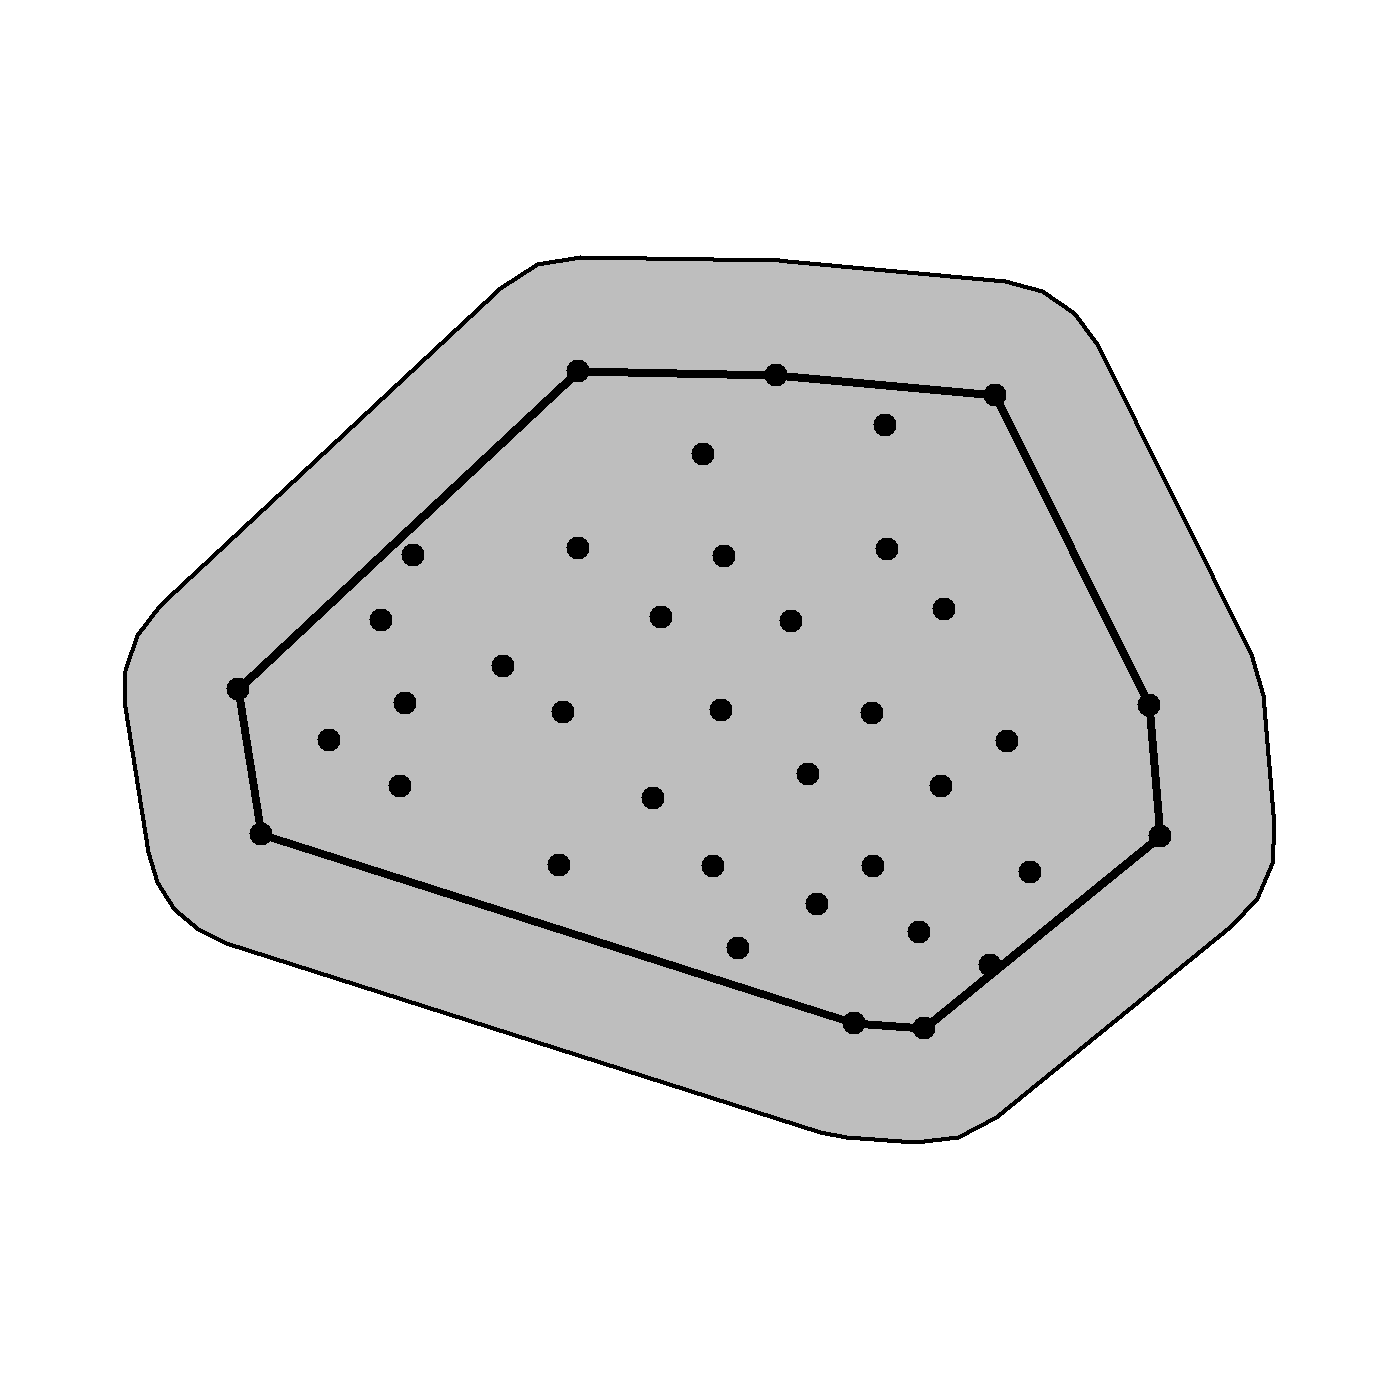
\includegraphics[height=3in,width=3in]{Ch3/figs/bufferedCH}
\end{center}
\caption{Convex hull of the bear hair snare array at Fort Drum, NY buffered by mean female
home range radius (2.19 km).}
\label{closed.fig.bch}
\end{figure}

To conjure up a
density estimate under model $M_0$, we compute the appropriate
posterior summary of the ratio of $N$ and the prescribed area ($277.011$ $km^2$):
{\small
\begin{verbatim}
> summary(fit0$sims.list$N/277.011)
   Min. 1st Qu.  Median    Mean 3rd Qu.    Max.
 0.1697  0.1733  0.1805  0.1803  0.1841  0.2130

> quantile(fit0$sims.list$N/277.011,c(0.025,0.975))
     2.5%     97.5%
0.1696684 0.1949381
\end{verbatim}
}
which yields a density estimate of about $0.18$ ind/km$^2$, and a $95\%$ Bayesian
confidence interval of $(0.170, 0.195)$.

In summary, we have an estimate of density if we have faith in our
stated value of the ``sample area''. Clearly though this is largely
subjective, and not something we can formally evaluate from the data.
How certain are we of this area? Can
we quantify our uncertainty about this quantity?
 More important, what exactly is
the meaning of this area and, in this context, how do we gauge bias
and/or variance of ``estimators'' of it? (i.e., what is it
estimating?).\footnote{Mention the delta approximation from
KARANTH AND NICHOLS (1998)?}
There is no theory to guide us in trying to answer these important questions.
XXX This is lame as shit XXXXX

\section{Temporally varying and behavioral effects}

The purpose of this chapter is mainly to emphasize the central
importance of the binomial model in capture-recapture and so we have
considered models for individual encounter frequencies - the number of
times individuals are captured out of $K$ samples.  Sometimes we can't
aggregate the encounter data for each individual, such as when
encounter probability varies over time among samples.  Time-varying
responses that are relevant in many capture-recapture studies are
``effort'' such as amount of search time, number of observers, or trap
nights, or when encounter probability varies over time or as a
function of date or season due to species behavior
\citep{kery_etal:2010}.  A common situation in many animal studies is
that in which there exists a ``behavioral response'' to trapping (even
if the animal is not physically trapped).
%For example, individuals might exhibit
%``trap happiness'' in response to baited traps. Conversely, individuals might learn
%to avoid traps (trap shyness) if the capture experience produces some negative
%stimulus.

Behavioral response is an important concept in animal studies
because individuals might learn to come to baited traps or avoid traps
due to trauma related to being encountered.  There are a number of
ways to parameterize a behavioral response to encounter. The
distinction between persistent and ephemeral was made by
\citet{yang_chao:2005} who considered a general behavioral response
model of the form:
\[
\mbox{logit}(p_{ik}) = \alpha_{0} + \alpha_{1}*y_{i,k-1} + \alpha_{2} x_{ik}
\]
where $x_{ik}$ is a covariate indicator variable of previous capture
(i.e., $x_{ik} = 1$ if captured in any previous period). Therefore,
encounter probability changes depending on whether an individual was
captured in the immediate previous period (ephemeral behavioral
response; \citep{yang_chao:2005}), described by the term
$\alpha_{1}*y_{i,k-1}$) or in any previous period (persistent behavioral
response).
%The former probably models a behavioral response due to
%individuals moving around their territory relatively slowly over time
%and the latter probably accommodates trap happiness due to baiting or
%shyness due to trauma.
Because spatial capture-recapture models allow us to include
trap-specific covariates, we can describe a 3rd type of behavioral
response -- a local behavioral response that is trap-specific
\citep{royle_etal:2011jwm}. In this local behavioral response, the
encounter probability is modified for an individual trap depending on
previous capture in that trap.

Models with temporal effects are easy to describe in the {\bf BUGS} language
and analyze and we provide a number of examples in
Chapt. \ref{chapt.covariates} and elsewhere.


\section{ Models with individual heterogeneity}
\label{closed.sec.modelmh}

Here we consider models with individual-specific encounter probability
parameters, say $p_{i}$, which we model according to some probability
distribution, $g(\theta)$. We denote this basic model assumption as
$p_{i} \sim g(\theta)$. This type of model is similar in concept to
extending a GLM to a GLMM but in the capture-recapture context $N$ is
unknown.  The basic class of models is often referred to as ``model
$M_h$'', but really this is a broad class of models, each being
distinguished by the specific distribution assumed for $p_{i}$.  There
are many different varieties of model $M_{h}$ including parametric and
various putatively non-parametric approaches
\citep{burnham_overton:1978, norris_pollock:1996, pledger:2000}. One
important practical matter is that estimates of $N$ can be extremely
sensitive to the choice of heterogeneity model
\citep{fienberg_etal:1999, dorazio_royle:2003, link:2003}. Indeed,
\citet{link:2003} showed that in some cases it's possible to find
models that yield precisely the same expected data, yet produce wildly
different estimates of $N$. In that sense, $N$ for most practical
purposes is not identifiable across classes of mixture models, and
this should be understood before fitting any such model. One solution
to this problem is to seek to model explicit factors that contribute
to heterogeneity, e.g., using individual covariate models (See
\ref{closed.sec.indcov} below). Indeed, spatial capture-recapture
models seek to do just that, by modeling heterogeneity due to the
spatial organization of individuals in relation to traps or other
encounter mechanism.  For additional background and applications of
model $M_{h}$ see \citet[][Chapt. 6]{royle_dorazio:2008} and
\citet[][Chapt. 6]{kery_schaub:2011}.

Model $M_{h}$ has important historical relevance to spatial
capture-recapture situations \citep{karanth:1995} because
investigators recognized that the juxtaposition of individuals with
the array of trap locations should yield heterogeneity in encounter
probability, and thus it became common to use some version of model $M_h$
in spatial trapping arrays to estimate $N$.  While this doesn't
resolve the problem of not knowing the area relevant to $N$, it does
yield an estimator that accommodates the heterogeneity in $p$ induced
by the spatial aspect of capture-recapture studies.

To see how this juxtaposition induces heterogeneity, we have to
understand the relevance of movement in capture-recapture models.
Imagine a quadrat that can be uniformly searched by a crew of
biologists for some species of reptile (see
\citet{royle_young:2008}).  Figure \ref{closed.fig.quadrat} shows a
sample quadrat searched repeatedly over a period of time. Further,
suppose that species exhibits some sense of spatial fidelity in the
form of a home range or territory, and individuals move about their
home range (home range centroids are given by the blue dots) in some
kind of random fashion.
%It is natural to think about it in terms of a
%movement process and sometimes that movement process can be modeled
%explicitly using hierarchical models \citep{royle_young:2008,
%  royle_etal:2011mee}.
Heuristically, we imagine that each individual in
the vicinity of the study area is liable to experience variable
exposure to encounter due to the overlap of its home range with the
sampled area - essentially the long-run proportion of times the
individual is within the sample plot boundaries, say $\phi$. We
might model the exposure of an individual to capture by supposing that
$z_{i} = 1$ if individual $i$ is available to be captured (i.e.,
within the survey plot) during any sample, and $0$ otherwise. Then,
$\Pr(z_{i}=1) = \phi$.  In the context of spatial studies, it is
natural that $\phi$ should depend on {\it where} an individual lives,
i.e., it should be individual-specific $\phi_{i}$
\citep{chandler_etal:2011}. This system describes, precisely, that of
``random temporary emigration'' \citep{kendall_etal:1997} where $\phi_{i}$
is the individual-specific probability of being ``available'' for
capture.

Conceptually, SCR models aim to deal with
this problem of variable exposure to sampling due to movement in the
proximity of the trapping array explicitly and formally with auxiliary
spatial information.  If individuals are detected with probability
$p_{0}$, {\it conditional} on $z_{i} = 1$, then the marginal
probability of detecting  individual $i$ is
\[
 p_{i} = p_{0}\phi_{i}
\]
so we see clearly that individual heterogeneity in encounter
probability is induced as a result of the juxtaposition of individuals
(i.e., their home ranges) with the sample apparatus and the movement
of individuals about their home range.

\begin{figure}
\begin{center}
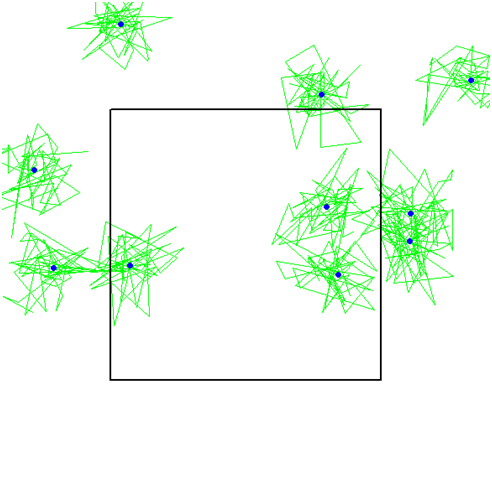
\includegraphics[height=3in]{Ch3/figs/quadrat}
\end{center}
\caption{A quadrat searched for lizards and the locations of each
  lizard over some period of time (simulated data).nice plot ! but, as usual, I would give more info. For instance, I would say something like ?Successive locations of 10 individual lizards over time are depicted by grey lines; black dots represent the individual activity centers.?}
\label{closed.fig.quadrat}
\end{figure}

We will work with a specific type of model $M_{h}$ here, that in which
we extend the basic binomial observation model of model $M_{0}$ so
that
\[
\mbox{logit}(p_{i}) = \mu + \eta_{i}
\]
where
\[
\eta_{i} \sim \mbox{Normal}(0, \sigma_{p}^2)
\]
We could as well write
\[
\mbox{logit}(p_{i}) \sim \mbox{Normal}(\mu,\sigma_{p}^2)
\]
This ``logit-normal mixture'' was analyzed by
\citet{coull_agresti:1999} and elsewhere. It is a natural extension of
the basic model with constant $p$, as a mixed GLMM, and similar models
occur throughout statistics. It is also natural to consider a beta
prior distribution for $p_{i}$ \citep{dorazio_royle:2003} and
so-called ``finite-mixture'' models are also popular
\citep{norris_pollock:1996, pledger:2000}. In the latter, individuals
are assumed to belong to a finite number of latent classes, each of
which has its own capture probability.


\subsection{Analysis of Model $M_h$}

If $N$ is known, it is worth taking note of the essential simplicity
of model $M_h$ as a binomial GLMM.  This is a type of model that is
widely applied throughout statistics using
standard methods of inference based either on integrated likelihood
\citep{laird_ware:1982, berger_etal:1999}, which we discuss in
Chapt. \ref{chapt.mle}, or standard Bayesian
methods. However, because $N$ is not known, inference is somewhat more
challenging. We address that here using Bayesian analysis based on
data augmentation (DA). Although we use data augmentation in the context of
Bayesian methods here, we note that
heterogeneity models formulated under DA are easily analyzed by
conventional likelihood methods as zero-inflated binomial mixtures
\citep{royle:2006} and more traditional analysis of model $M_h$ based on
integrated likelihood, without using data augmentation, has been
considered by \citet{coull_agresti:1999}, \citet{dorazio_royle:2003},
and others.

As with model $M_{0}$, we have the Bernoulli model for the
zero-inflation variables: $z_{i} \sim \mbox{Bern}(\psi)$ and the model
of the observations expressed conditional on these latent variables
$z_{i}$. For $z_{i}=1$, we have a binomial model with
individual-specific $p_{i}$:
\[
y_{i}|{z_{i} \! = \! 1} \sim \mbox{Bin}(K,p_{i})
\]
and otherwise $y_{i} |{ z_{i} \! = \! 0} \sim \delta(0)$. Further, we
prescribe a distribution for $p_{i}$. Here we assume
\[
\mathrm{logit}(p_{i}) \sim \mbox{Normal}(\mu,\sigma^2)
\]
For prior distributions we assume
$p_{0} = \mbox{logit}^{-1}(\mu) \sim
\mbox{Unif}(0,1)$ and, for the variance component
$\sigma \sim \mbox{Unif}(0,B)$ for some large $B$.
\begin{comment}
The basic {\bf BUGS} description for this model is given as follows:
{\small
\begin{verbatim}
model{

p0 ~ dunif(0,1)       # prior distributions
mup<- log(p0/(1-p0))
sigmap ~ dunif(0,10)
taup<- 1/(sigmap*sigmap)
psi~dunif(0,1)

for(i in 1:(nind+nz)){
  z[i]~dbern(psi)     # zero inflation variables
  lp[i] ~ dnorm(mup,taup) # individual effect
  logit(p[i])<-lp[i]
  mu[i]<-z[i]*p[i]
  y[i]~dbin(mu[i],K)  #  observation model
 }

N<-sum(z[1:(nind+nz)])  # N is a derived parameter
}
\end{verbatim}
}
\end{comment}
Another common default prior is to assume
$\tau = 1/\sigma^{2} \sim \mbox{Gamma}(.1,.1)$, although we usually
choose the $\sigma \sim \mbox{Unif}(0,B)$.



\subsection{Analysis of the Fort Drum data}
\label{closed.sec.Mhbear}
The logit-normal heterogeneity model was fitted to the bear data from
the Fort Drum study, and we used data augmentation to produce a data
set of $M=500$ individuals.  We ran the model using {\bf JAGS} with
the instructions given as follows:
{\small
\begin{verbatim}
[... get data as before ....]

set.seed(2013)

cat("
model{
p0 ~ dunif(0,1)       # prior distributions
mup<- log(p0/(1-p0))
sigmap ~ dunif(0,10)
taup<- 1/(sigmap*sigmap)
psi~dunif(0,1)

for(i in 1:(nind+nz)){
  z[i]~dbern(psi)     # zero inflation variables
  lp[i] ~ dnorm(mup,taup) # individual effect
  logit(p[i])<-lp[i]
  mu[i]<-z[i]*p[i]
  y[i]~dbin(mu[i],K)  #  observation model
 }

N<-sum(z[1:(nind+nz)])
}
",file="modelMh.txt")

data1<-list(y=ytot, nz=nz, nind=nind,K=K)
params1= c('p0','sigmap','psi','N')
inits =  function() {list(z=as.numeric(ytot>=1), psi=.6, p0=runif(1),
          sigmap=runif(1,.7,1.2),lp=rnorm(M,-2)) }

library("rjags")
jm<- jags.model("modelMh.txt", data=data1, inits=inits, n.chains=3,
                 n.adapt=10000)
jout<- coda.samples(jm, params1, n.iter=500000, thin=1)
\end{verbatim}
}
This produces the posterior distribution for $N$ shown
in Fig. \ref{closed.fig.bearMh}. Posterior summaries of parameters are
given as follows:
{\small
\begin{verbatim}
summary(jout)

[... output deleted ...]
Iterations = 500001:1e+06
Thinning interval = 1
Number of chains = 3
Sample size per chain = 5e+05

1. Empirical mean and standard deviation for each variable,
   plus standard error of the mean:

            Mean       SD  Naive SE Time-series SE
N      119.11050 57.85859 4.724e-02       1.285748
p0       0.07228  0.05545 4.527e-05       0.001064
psi      0.23928  0.11669 9.528e-05       0.002562
sigmap   2.08650  0.53532 4.371e-04       0.010903

xxxxxx
Could you explain this output a little more ? I later saw that you do
later on, but I would always explain new stuff where it first
appears. For instance, I had no clue what the naive SE meant ? Seems
to be the Monte Carlo error ?
xxxxxxxx

[... output deleted ... ]
\end{verbatim}
}

We used $M=500$ for this analysis and we
note that  while the posterior mass of $N$ is concentrated away from this
upper bound (Fig. \ref{closed.fig.bearMh}), the posterior has an
extremely long right tail, with some posterior values at the upper
bound $N=500$, suggesting that an even higher value of $M$ may be
called for.

To characterize the posterior distribution of density we produce the
relevant summaries of the posterior distribution of $N/277.11$ where,
recall, the buffered area of the convex hull is 277.11 $km^2$:
{\small
\begin{verbatim}
N<-c(jout[[1]][,"N"],jout[[2]][,"N"],jout[[3]][,"N"])
 summary(N/277.11)
   Min. 1st Qu.  Median    Mean 3rd Qu.    Max.
 0.1696  0.2959  0.3681  0.4298  0.4908  1.8040
> quantile(N/277.11,c(0.025,0.50,0.975))
     2.5%       50%     97.5%
0.2237379 0.3680849 1.0284724
\end{verbatim}
}
so the point estimate, characterized by the posterior mean, is around
$0.43$ bears per square km and a 95\% Bayesian credible interval is
$(0.224, 1.028)$.


The model runs effectively in {\bf WinBUGS} but sometimes with apparently
inefficient mixing for reasons that may be related to bad starting
values. In some cases this was resolved if we supplied starting values
for the $logit(p_{i})$ parameters and $\tau$. We provide a user-friendly {\bf R}
function \mbox{\tt modelMhBUGS} in the package \mbox{\tt scrbook} which will
fit the model using either {\bf JAGS} or {\bf WinBUGS} as specified by
the user.
In addition, for fun, we construct our own MCMC algorithm using a Metropolized
Gibbs sampler for model $M_{h}$ in Chapt. \ref{chapt.mcmc}, where we
also develop the MCMC  algorithms for spatial capture-recapture models.


\subsection{Comparison with MLE}

Because of the skewed posterior we see that the posterior mean
($N=119$) is considerably higher than the posterior median
($N=102$). Moreover, posterior summaries are estimated with a
relatively high error: The ``Time-series'' or Monte Carlo SE of around
1.2 (see secs.  for discussion of this quantity
\ref{glms.sec.convergence} \ref{mcmc.sec.mcmcsummary}) even despite
the high number of iterations we ran here (each of 3 chains based on
500000 iterations).  Further, it may be surprising that the posterior
mode does not compare well with the MLE which we presented in
sec. XXXX chapter 1 XXXXX which was XXXXXX.
To see this, we compute the posterior model by finding
the posterior value of $N$ with the highest mass, which is a
relatively easy proposition because $N$ is discrete.
 But we want to smooth out some of the Monte
Carlo error a bit so we used a smoothing spline to the posterior
frequencies of $N$ as follows (here we take only the first 80 values):
\begin{verbatim}
  tt<-table(jout[[1]][,"N"])[1:80]
  xg<-as.numeric(names(tt))
  plot(xg,tt)
  sp<- smooth.spline(xg,tt,df=9)
  sp$x[sp$y==max(sp$y)]
[1] 81
\end{verbatim}
The \mbox{\tt df} argument controls the degree of smoothing and we
find in this case that the modal value (i.e., 81) is not too sensitive
to the smoothing parameter but this should be checked in any specific
instance\footnote{we need to give examples of using \mbox{\tt
    density()} to obtain modes}.
To compare this with the MLE, we used
the {\bf R} code contained in Panel 6.1 from \citet{royle_dorazio:2008}.  The
MLE of $log(n_{0})$, the logarithm of the number of uncaptured
individuals, is $\widehat{log(n0)} = 3.86$ and therefore $\hat{N} =
exp(3.86)+47 = 94.47$ which is not at all consistent with the
mode in
Fig. \ref{closed.fig.bearMh}.
%\footnote{We note that the result is inconsistent with Gardner et
%  al. (2009) who reported an MLE of 104.1 ($density = 0.437
%  inds/km^2$) although we do not know the reason for this at the
%  present time.}
%To convert this to density we use the buffered area
%as computed above (255.3 $km^2$)\footnote{WRONG \#} and perform the
%required summary analysis on the posterior samples of $N$, which
%results in about $0.37$ individuals/$km^2$. The reader should carry
%out this analysis to confirm the estimates, and also obtain the $95\%$
%confidence interval.
\begin{comment}
We reflect for a moment on the whole idea of using
capture-recapture to estimate density. It seems pointless to argue about ``buffer width'' when
we can't even decide on an estimate of $N$! Maybe this reflects poorly
on the desire to have a point estimate of a quantity more than our
ability to provide
\end{comment}

{\bf Remarks:}
First of all the posterior for this model and data set is
very sensitive to prior distributions. While MLEs are invariant to
transformation of the parameters, the posterior distribution
definitely is {\it not} invariant. In the present case, the use of a
$\mbox{Unif}(0,1)$ prior for $p_{0} = \mbox{expit}(\mu)$ is somewhat
informative -- in particular, it is not at all ``flat'' on the scale
of $\mu$ -- and this affects the posterior.  We generally always
recommend use of a $\mbox{Unif}(0,1)$ prior for $\mbox{expit}(\mu)$ in such
models. That said, we were surprised at this result, and we
experimented with other prior configurations including putting a flat
prior on $\mu$ directly. That specific prior suggests the possibility
that the posterior distribution may be improper for that prior
specification. This kind of small sample instability has been widely
noted in model $M_h$ \citep{fienberg_etal:1999, dorazio_royle:2003},
as has extreme sensitivity to the specific form of model $M_{h}$ \citep{link:2003}.
In summary, while the mode is well-defined, the data set is relatively
sparse and hence inferences are poor and sensitive to model choice.

\begin{figure}
\centering
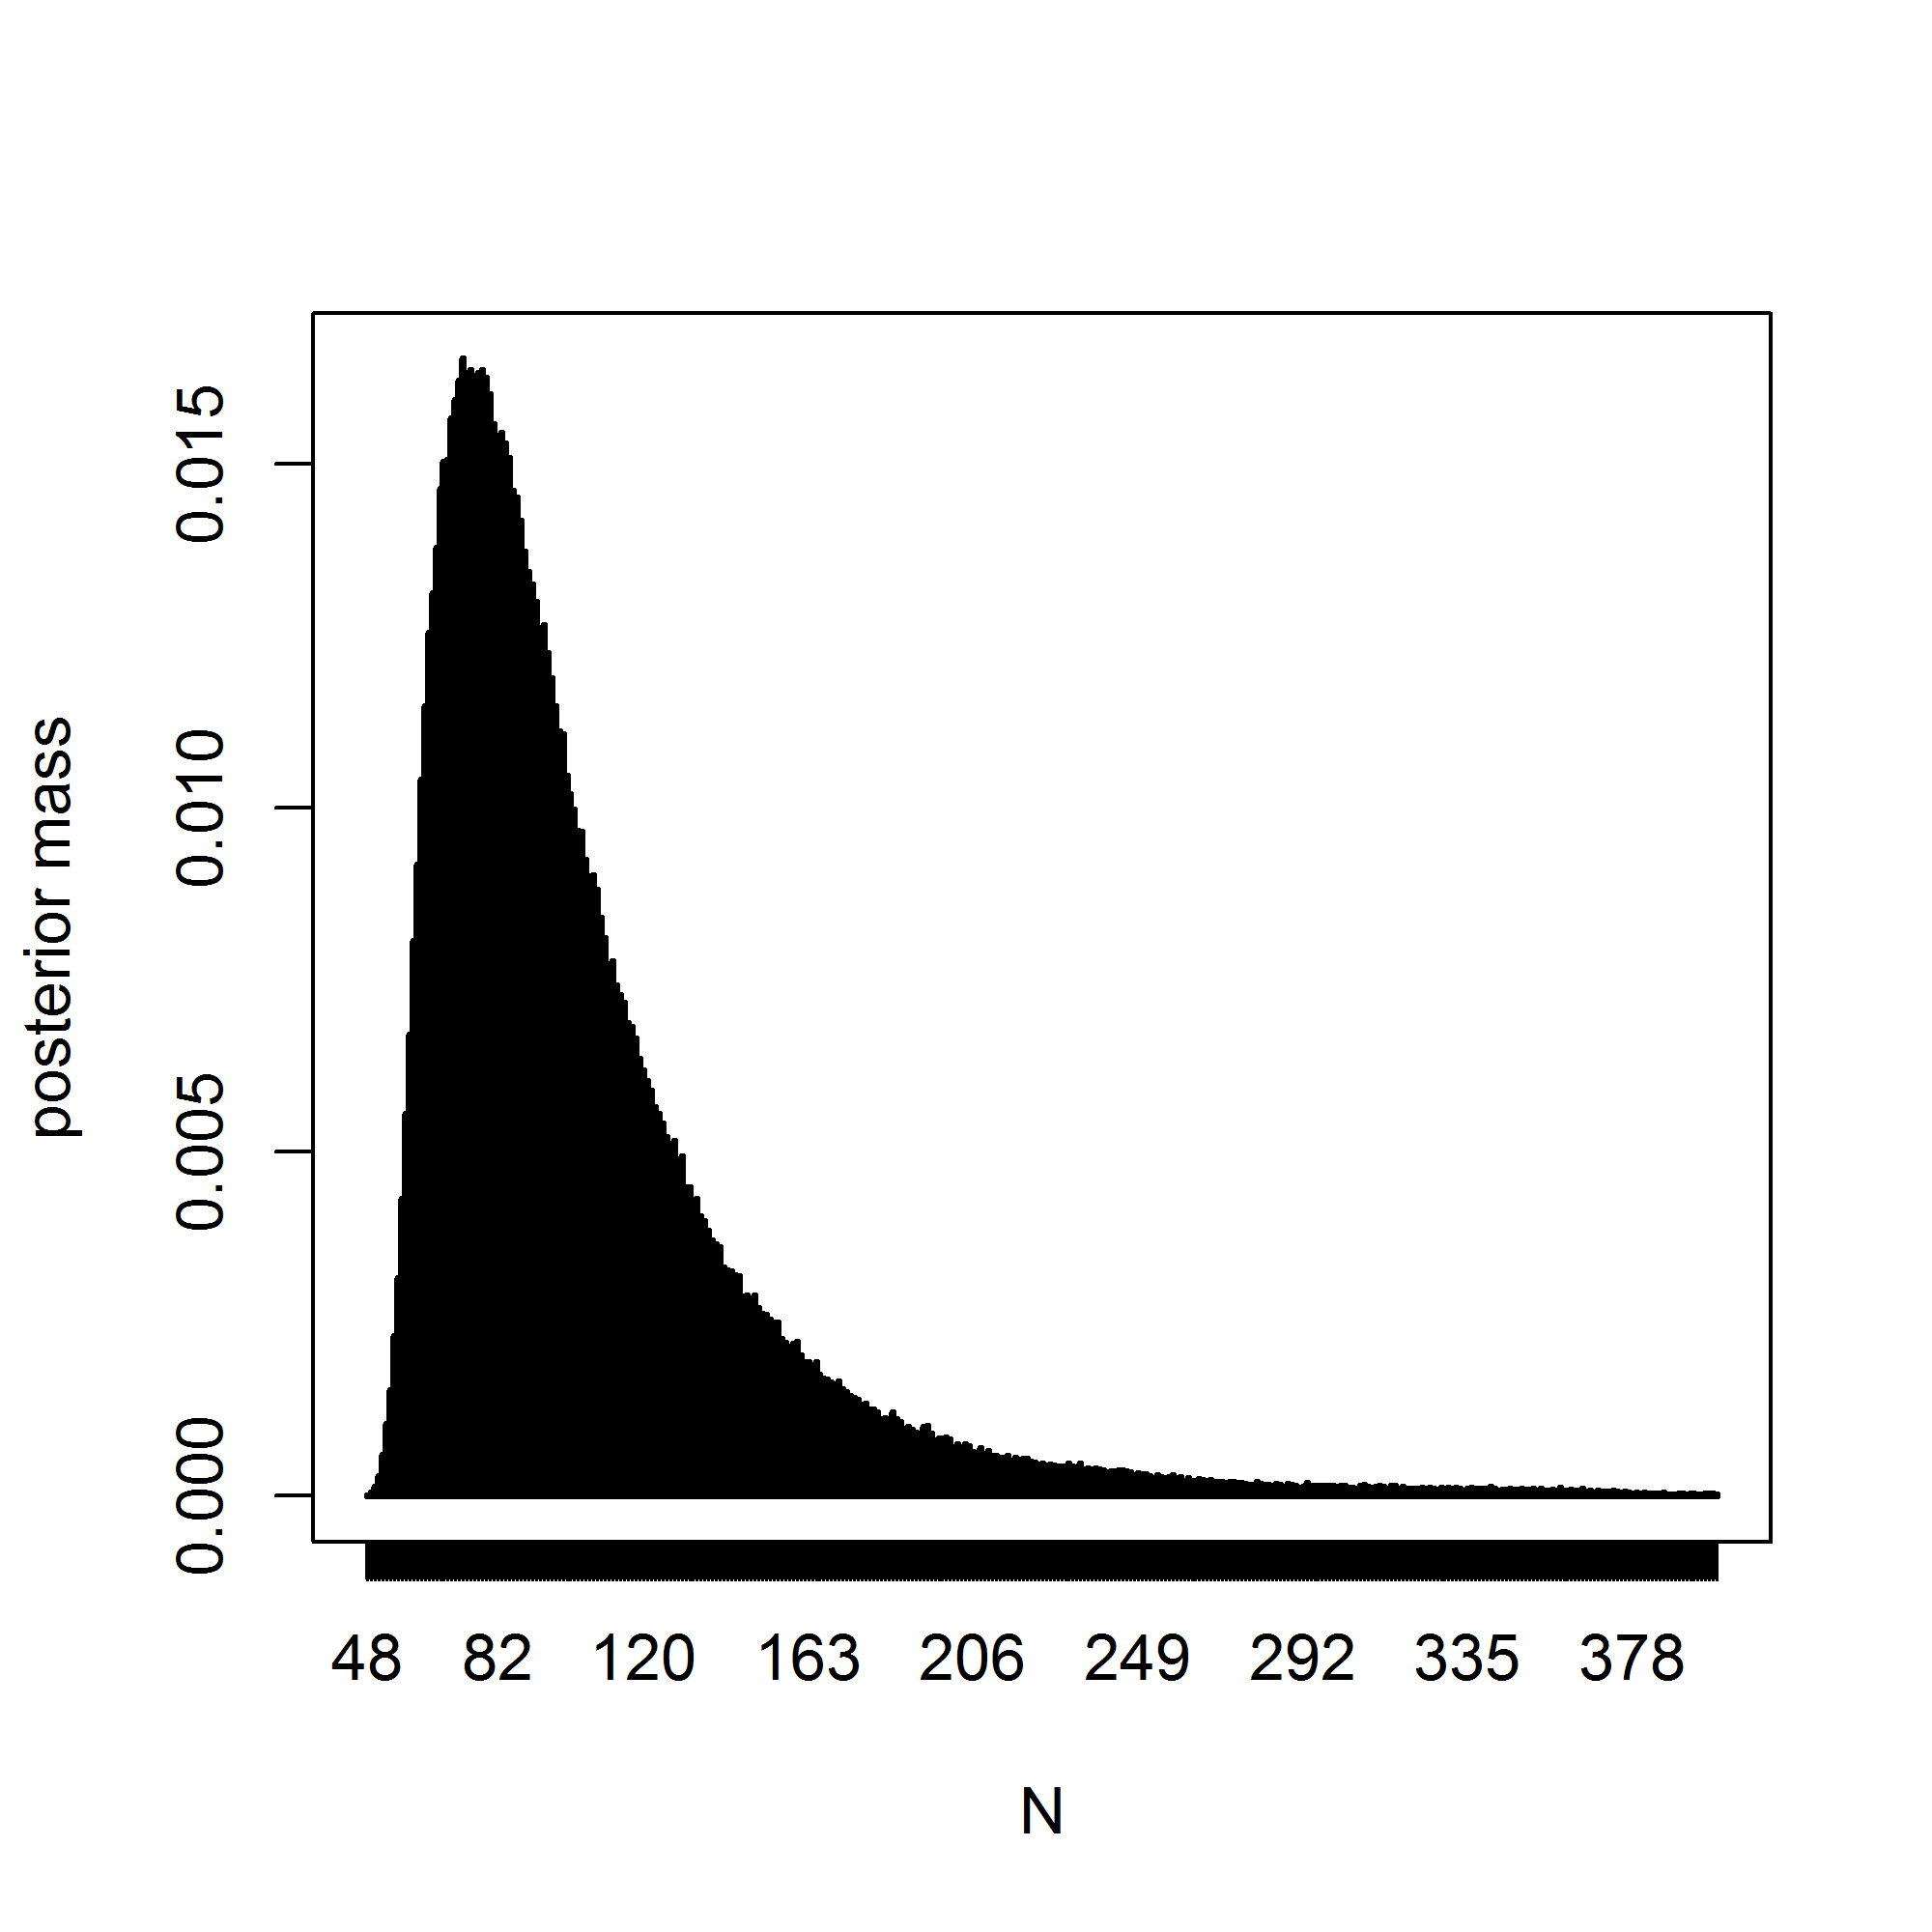
\includegraphics[height=4.5in,width=4.5in]{Ch3/figs/bear-modelMh-post}
\caption{Posterior of $N$ for Fort Drum bear study data under the
logit-normal version of model $M_h$.
}
\label{closed.fig.bearMh}
\end{figure}




\begin{comment}

To begin, we first collect all of our model components
which are as follows: $[y_{i}| p_{i},z_{i}]$,
$[p_{i}|\mu_{p},\sigma_{p}]$, and $[z_{i}|\psi]$
for {\it each} $i=1,2,\ldots,M$ and then prior distributions
$[\mu_{p}]$, $[\sigma_{p}]$ and $[\psi]$.
The joint posterior distribution of all unknown quantities in the model
is proportional to the joint distribution of all elements
$y_{i},p_{i},z_{i}$ and also the prior distributions of the prior parameters:
\[
\left\{ \prod_{i=1}^{M} [y_{i}|p_{i},z_{i}][p_{i}|\mu_{p},\sigma_{p}]
[z_{i}|\psi] \right\} [\mu_{p},\sigma_{p},\psi]
\]
For prior distributions, we assume that $\mu_{p},\sigma_{p}, \psi$ are
mutually independent and for $\mu_{p}$ and $\sigma_{p}$ we use
improper uniform priors, and $\psi \sim \mbox{Unif}(0,1)$.  Note that
the likelihood contribution for each individual, when conditioned on
$p_{i}$ and $z_{i}$, does not depend on $\psi$, $\mu_{p}$, or
$\sigma_{p}$.  As such, the full-conditionals for the structural
parameters $\psi$ only depends on the collection of data augmentation
variables $z_{i}$, and that for $\mu_{p}$ and $\sigma_{p}$ will only
depends on the collection of latent variables $p_{i}; i=1,2,\ldots,M$.
The full conditionals for all the unknowns are as follows:

{\bf (1)} For $p_{i}$:
\begin{eqnarray*}
[p_{i}|y_{i}, \mu_p, \sigma_{p},z_{i}=1] &\propto  &
[y_{i}|p_{i}][p_{i}|\mu_p,\sigma_{p}^{2}] \mbox{ if $z_{i}=1$ }  \\
                 &  &  [p_{i}|\mu_p,\sigma_{p}] \mbox{if $z_{i}=0$ }
\end{eqnarray*}

{\bf (2)} for $z_{i}$:
\[
z_{i} | \cdot \propto [y_{i}|z_{i}*p_{i}] \mbox{Bern}(z_{i}|\psi)
\]

{\bf (3)} For $\mu_{p}$:
\[
[\mu_{p} | \cdot ] \sim \prod_{i} [p_{i}| \cdot] *\mbox{const}
\]


{\bf (4)} For $\sigma_{p}$:
\[
[ \sigma_{p}|\cdot ] \sim\prod_{i}[p_{i}| \cdot ]*\mbox{const}
\]

{\bf (5)} For $\psi$:
\[
\psi|\cdot\sim \mbox{Beta}(1 + \sum z_{i}, 1 + M - \sum z_{i})
\]


We've  identified each of the full conditional
distributions in sufficient detail to apply the
Metropolis-Hastings algorithm. With the exception of $\psi$ which has
a convenient analytic solution -- it is a beta distribution which we
can easily sample directly. In truth, we could also sample $\mu_{p}$
and $\sigma_{p}^{2}$ directly with certain choices of prior
distributions. For example, if $\mu_{p} \sim \mbox{Normal}(0, 1000)$
then the full conditional for $\mu_{p}$ is also normal, etc..
We implement an MCMC algorithm for this model in the following block
of {\bf R} code.  The basic structure is: initialize the parameters
and create any required output or intermediate data holders, and then
begin the main MCMC loop which, in this case, generates 100000
samples.\footnote{This data grabbing function is not implemented yet}

{\small
\begin{verbatim}
## obtain the bear data by executing the previous data grabbing
## function

temp<-getdata()
M<-temp$M
K<-temp$K
ytot<-temp$ytot

###
### MCMC algorithm for Model Mh

out<-matrix(NA,nrow=100000,ncol=4)
dimnames(out)<-list(NULL,c("mu","sigma","psi","N"))
lp<- rnorm(M,-1,1)
p<-expit(lp)
mu<- -1
p0<-exp(mu)/(1+exp(mu))
sigma<- 1
psi<- .5
z<-rbinom(M,1,psi)
z[ytot>0]<-1

for(i in 1:100000){

### update the logit(p) parameters
lpc<- rnorm(M,lp,1)  # 0.5 is a tuning parameter
pc<-expit(lpc)
lik.curr<-log(dbinom(ytot,K,z*p)*dnorm(lp,mu,sigma))
lik.cand<-log(dbinom(ytot,K,z*pc)*dnorm(lpc,mu,sigma))
kp<- runif(M) < exp(lik.cand-lik.curr)
p[kp]<-pc[kp]
lp[kp]<-lpc[kp]

p0c<- rnorm(1,p0,.05)
if(p0c>0 & p0c<1){
muc<-log(p0c/(1-p0c))
lik.curr<-sum(dnorm(lp,mu,sigma,log=TRUE))
lik.cand<-sum(dnorm(lp,muc,sigma,log=TRUE))
if(runif(1)<exp(lik.cand-lik.curr)) {
 mu<-muc
 p0<-p0c
}
}

sigmac<-rnorm(1,sigma,.5)
if(sigmac>0){
lik.curr<-sum(dnorm(lp,mu,sigma,log=TRUE))
lik.cand<-sum(dnorm(lp,mu,sigmac,log=TRUE))
if(runif(1)<exp(lik.cand-lik.curr))
 sigma<-sigmac
}

### update the z[i] variables
zc<-  ifelse(z==1,0,1)  # candidate is 0 if current = 1, etc..
lik.curr<- dbinom(ytot,K,z*p)*dbinom(z,1,psi)
lik.cand<- dbinom(ytot,K,zc*p)*dbinom(zc,1,psi)
kp<- runif(M) <  (lik.cand/lik.curr)
z[kp]<- zc[kp]

psi<-rbeta(1, sum(z) + 1, M-sum(z) + 1)

out[i,]<- c(mu,sigma,psi,sum(z))
}
\end{verbatim}
}


{\bf Remarks}: (1) for parameters with bounded support, i.e.,
$\sigma_{p}$ and $p_{0}$, we are using a random walk candidate
generator but rejecting draws outside of the parameter space.  (2) We
mostly use Metropolis-Hastings except for the data augmentation
parameter $\psi$ which we sample directly from its full-conditional
distribution which is a beta distribution.  (3) Even the latent data
augmentation variables $z_{i}$ are updated using Metropolis-Hastings
although they too can be updated directly from their full-conditional.
\end{comment}


\begin{comment}

\subsection{Exercises related to model $M_h$}

\begin{itemize}
\item[(1)] Enclose the MCMC algorithm in an R function and provide
  arguments for some of the parameters of the function that a user
  might wish to modify.
\item[(2)] Execute the function and compare the results to those
  generated from WinBUGS in the previous section
\item[(3)] Note that the prior distribution for the ``mean'' parameter
  is given on $p_0=exp(\mu)/(1+exp(\mu))$.  Reformulate the algorithm
  with a flat prior on $\mu$ and see what happens. Contemplate this.
\item[(4)] Using Bayes rule, figure out the full conditional for
  $z_{i}$ so that you don't have to use MH for that one. It might be
  more efficient. Is it?
\item[(5)] Modify the MCMC algorithm so that the prior for $\mu_{p}$
  is an improper flat prior. i.e., $[\mu_{p}] \propto 1$. Describe the
  posterior distribution of $N$.
\end{itemize}

\end{comment}



\section{Individual Covariate Models: Toward Spatial Capture-Recapture}
\label{closed.sec.indcov}


A standard situation in capture-recapture models is when a
covariate which is thought
 to influence
encounter probability is measured for each individual.
As with other closed population models, we
begin with the basic binomial observation model:
\[
y_{i} \sim \mbox{Bin}(K, p_{i})
\]
and we assume also  a model for encounter probability according to:
\begin{equation}
 \mbox{logit}(p_{i}) = \alpha + \beta x_{i}
\label{closed.eq.ha}
\end{equation}
Classical examples of covariates influencing detection probability are
type of animal (juvenile/adult or male/female), a continuous covariate
such as body mass \citep[][ch. 6]{royle_dorazio:2008}, or a
discrete covariate such as group or cluster size. For example, in
models of aerial survey data, it is natural to model the detection
probability of a group as a function of the observation-level individual
covariate, ``group size'' \citep{royle:2008, royle:2009,
  langtimm_etal:2011}.

Such ``individual covariate models'' are similar in structure to model
$M_{h}$, except that the individual effects are {\it observed} for the
$n$ individuals that appear in the sample. These models are important
here because spatial capture-recapture models can be descrived precisely as a form of
individual covariate model, an idea that we will develop here and
elsewhere. Specifically, they are such models, but where the
individual covariate is a partially observed latent variable for
captured individuals. As such, it is a type of measurement error.
That is, unlike model $M_h$, we do have some direct information about the
latent variable, which comes from the spatial locations/distribution
of individual recaptures.

Traditionally, estimation of $N$ in individual covariate models is
achieved using methods based on ideas of unequal probability sampling
(i.e., Horvitz-Thompson estimation\footnote{For a  quick summary of
  the idea see:
  \url{http://en.wikipedia.org/wiki/Horvitz-Thompson_estimator}};
%see
\citet{huggins:1989},
\citet{alho:1990} and \citet{borchers_etal:2002}). An estimator of $N$ is
\[
\hat{N} = \sum_{i}^{n} \frac{1}{\tilde{p}_{i}}
\]
where $\tilde{p}_{i}$ is the probability that individual $i$ appeared
in the sample.  That is, $\tilde{p}_{i} = \Pr(y_{i}>0)$
where, in closed population capture-recapture models,
\[
\Pr(y_{i}>0) = (1- (1-p_{i})^K)
\]
where $p_{i}$ is a function of parameters $\alpha$ and $\beta$
according to Eq. \ref{closed.eq.ha}.  In practice, parameters are
estimated from the conditional-likelihood of the observed encounter
histories which is, for observation $y_{i}$,
\[
{\cal L}_{c}(\alpha, \beta | y_{i}) = \frac{ \mbox{Bin}(y_{i}|\alpha,\beta) } { \tilde{p}_{i}}.
\]

Here we take a formal model-based approach to Bayesian analysis of
such models based on the joint likelihood
using data augmentation \citep{royle:2009}. Classical
likelihood analysis of the so-called ``full likelihood'' is covered
 by \citet{borchers_etal:2002}.  For Bayesian analysis of
individual covariate models, because the individual covariate is
unobserved for the $N-n$ uncaptured individuals, we require a model to
describe variation among individuals, essentially allowing the sample
to be extrapolated to the population.  For our present purposes, we
consider a continuous covariate and we assume that it has a normal
distribution:
\[
x_{i} \sim \mbox{Normal}(\mu,\sigma^{2})
\]
Data augmentation can be applied directly to this class of models. In
particular, reformulation of the model under DA yields a basic
zero-inflated binomial model of the form:
\begin{eqnarray*}
z_{i} &\sim& \mbox{Bern}(\psi) \; \; \; i=1,2,\ldots,M\\
y_{i}|{z_{i}\! =\! 1} &\sim& \mbox{Bin}(K,p_{i}(x_{i})) \\
y_{i} |{ z_{i}\! =\! 0} &\sim& \delta(0)  \\
x_{i} & \sim & \mbox{Normal}(\mu,\sigma^{2})
\end{eqnarray*}
Fully spatial capture-recapture models use this
formulation with a latent covariate that is directly related to the
individual detection probability (see next section). As with the
previous models, implementation is trivial in the {\bf BUGS} language. The
{\bf BUGS} specification is very similar to that for model $M_h$, but we
require the distribution of the covariate to be specified, along with
priors for the parameters of that distribution.


\subsection{Example: Location of capture as a covariate.}

Here we consider a special type of individual covariate model that is
especially relevant to SCR.
If we had a regular grid of traps over some geographic region,
then we imagine that the average location of capture would be a decent
estimate (heuristically) of an individual's home range center.
Intuitively, some measure of typical distance from home range center to
traps for an individual should therefore be a reasonable  covariate to explain
heterogeneity in encounter probability, i.e., individuals with more
exposure to traps should have higher encounter probabilities and vice
versa.  A version of this idea was put forth by
\citet{boulanger_mclellan:2001} (see also \citet{ivan:2012}), but
using the Huggins-Alho estimator and with covariate ``distance to
edge'' of the trapping array. A limitation of this  approach is
that it does not provide a solution to the problem that the trap area
is fundamentally ill-defined, nor does it readily accommodate the
inherent and heterogeneous variation in this measured covariate.

We provide an example of this type of heuristically motivated
approach using a fully model-based individual covariate model
described above analyzed by data augmentation. We take a slightly
different approach than that adopted by
\citet{boulanger_mclellan:2001}. By analyzing the full likelihood and
placing a prior distribution on the individual covariate, we resolve
the problem of having an ill-defined area over which the population
size is distributed. After you read later chapters of this book, it
will be apparent that SCR models represent a formalization of this
heuristic procedure.

For our purposes here, we define $x_{i} = ||{\bf s}_{i} - {\bf
  x}_{0}||$ where ${\bf s}_{i}$ is the average encounter location of
individual $i$ and ${\bf x}_{0}$ is the centroid of the trap array.
Conceptually, individuals in the middle of the array should have a
higher probability of encounter and, as $x_{i}$ increases, $p_{i}$
should therefore decrease. We note that we have defined ${\bf s}_{i}$
in terms of a sample quantity - the observed mean - which is ad hoc
but consistent with existing applications in the literature.  For an
expansive, dense trapping grid we might expect the sample mean
encounter location to be a good estimate of home range center but,
clearly this is biased for individuals that live around the edge (or
off) the trapping array. Regardless, it should be good enough for our
present purposes of demonstrating this heuristically appealing
application of an individual covariate model. A key point is that
${\bf s}_{i}$ is missing for each individual that is not encountered
and so  $x_{i}$ is also missing. Therefore, it is a latent variable, or random
effect, and we need therefore to specify a probability distribution
for it.  As a measurement of distance we know it must be
positive-valued, and it seems sensible that an individual located
extremely far from the array of traps would not be captured.
Therefore,
 lets assume that $x_{i}$ is uniformly distributed from $0$ to some large number,
say $D_{max}$, beyond which it would be difficult to imagine an
individual being captured. For example, $D_{max}$ should be at a home
range diameter past the furthest trap from the center.  As such, we
use this distribution for the individual covariate ``distance from
center of the trap array''
\[
 x_{i} \sim \mbox{Unif}(0,D_{max})
\]
where $D_{max}$ is a specified constant, which we may choose to be
arbitrarily large.  In practice, people have
used distance from edge of the trap array but that is less easy to
make sense of.


\subsection{Fort Drum Bear Study}


We have to do a little bit of data processing to fit this individual
covariate model to the Fort Drum data.  We need to compute the
individual covariate ${\bf x}_{i}$ (distance from the centroid of the
trapping array) using the {\bf R} function \mbox{\tt spiderplot}
provided in \mbox{\tt scrbook}. This function also produces the keen
plot shown in Fig. \ref{closed.fig.spiderplot} which we call a
``spider plot''.  The {\bf R} commands for obtaining the individual
covariate ``distance from trap centroid'' and making the spider plot
are as follows:
\begin{verbatim}
library("scrbook")
data("beardata")
toad<- spiderplot(beardata$bearArray,beardata$trapmat)
xcent<-toad$xcent
\end{verbatim}
\begin{figure}
\centering
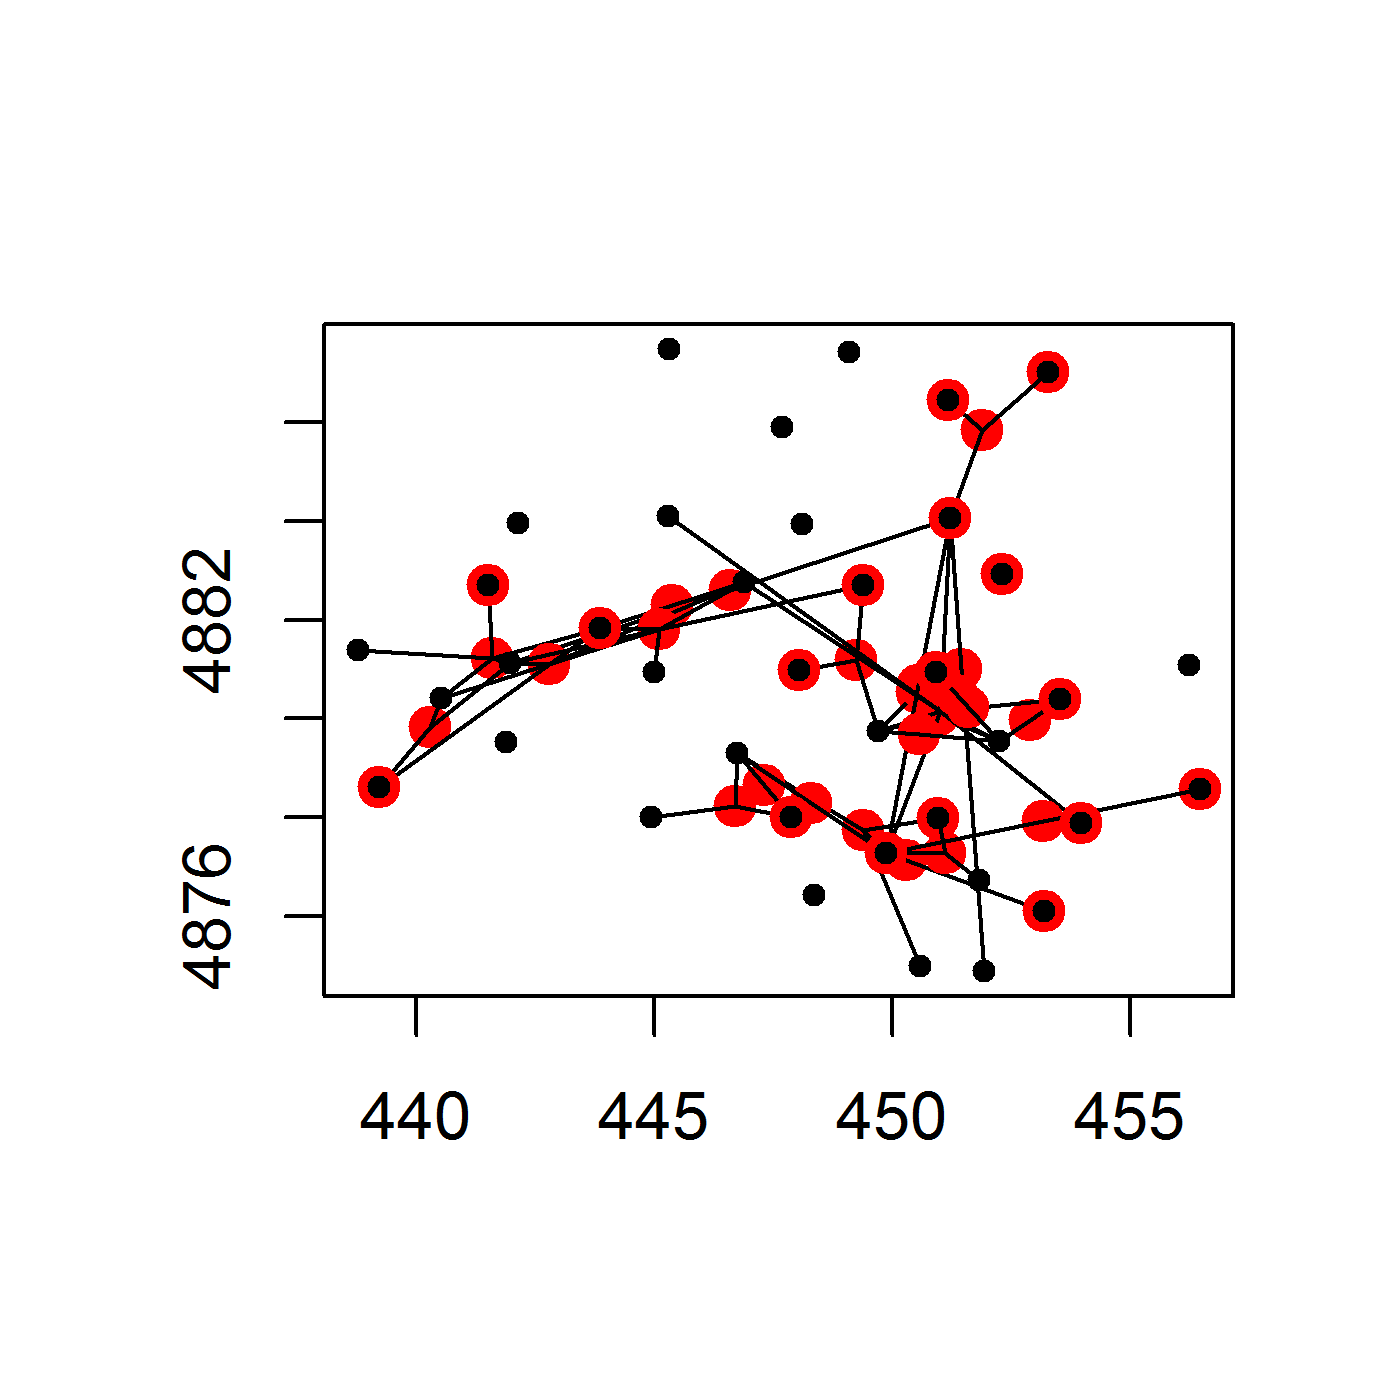
\includegraphics[height=3.5in,width=3.5in]{Ch3/figs/bear_spiderplot.png}
\caption{Spider plot of the Fort Drum study data.
The black dots represent the 47 trap locations with larger red dots
being the average capture location of each bear. i.e., its estimated home
range center. All traps in which a bear was captured are connected to
its estimated home range center with a line.
XXX note change one of the dots to an X or something XXXXX
}
\label{closed.fig.spiderplot}
\end{figure}

For the analysis of these data using the individual covariate
"distance from centroid" we used $x_{i} \sim \mbox{Unif}(0,D_{max})$
with $D_{max} = 11.5$ $km^2$, which is about the distance from the
array center to the furthest trap.  Once we pick $D_{max}$ then the
direct implication is that the population size parameter applies to
the area within 11.5 units of the trap centroid and thus we will find
that $N$ does, in fact, scale with our choice of $D_{max}$ to reflect
the changing area over which the $N$ individuals of the model reside.
The {\bf BUGS} model specification and {\bf R} commands to package the
data and fit the model are as follows:
{\small
\begin{verbatim}
cat("
model{
p0 ~ dunif(0,1)       # prior distributions
mup<- log(p0/(1-p0))
psi~dunif(0,1)
beta~dnorm(0,.01)

for(i in 1:(nind+nz)){
  xcent[i]~dunif(0,Dmax)
  z[i]~dbern(psi)     # DA variables
  lp[i] <- mup + beta*xcent[i] # individual effect
  logit(p[i])<-lp[i]
  mu[i]<-z[i]*p[i]
  y[i]~dbin(mu[i],K)  #  observation model
 }
N<-sum(z[1:(nind+nz)])
}
",file="modelMcov.txt")

data2<-list(y=ytot,nz=nz,nind=nind,K=K,xcent=xcent,Dmax=11.5)
params2<-list('p0','psi','N','beta')
inits =  function() {list(z=zst, psi=psi, p0=runif(1),beta=rnorm(1) ) }
fit2 =   bugs(data2, inits, params2, model.file="modelMcov.txt",working.directory=getwd(),
         debug=T, n.chains=3, n.iter=11000, n.burnin=1000, n.thin=1)
\end{verbatim}
}
This produces the following posterior summary statistics:
{\small
\begin{verbatim}
Inference for Bugs model at "modelMcov.txt", fit using WinBUGS,
 3 chains, each with 11000 iterations (first 1000 discarded)
 n.sims = 30000 iterations saved
           mean    sd   2.5%    25%    50%    75%  97.5% Rhat n.eff
p0         0.54  0.07   0.40   0.50   0.54   0.59   0.67    1  1100
psi        0.34  0.05   0.25   0.31   0.34   0.37   0.44    1  3500
N         58.92  5.49  50.00  55.00  58.00  62.00  71.00    1  1900
beta      -0.25  0.06  -0.36  -0.29  -0.25  -0.21  -0.12    1   780
deviance 459.51 13.21 435.80 450.20 458.80 467.90 487.40    1  2600
\end{verbatim}
}

It might be
perplexing that the estimated $N$ is much lower than obtained by model
$M_h$ but there is a good explanation for this, discussed
subsequently. That issue notwithstanding, it is worth pondering how
this model could be an improvement (conceptually or technically) over
some other model/estimator including $M_0$ and $M_h$ considered
previously. Well, for one, we have accounted formally for
heterogeneity due to spatial location of individuals relative to
exposure to the trap array, characterized by the centroid of the
array. Moreover, we have done so using a model that is based on an
explicit mechanism, as opposed to a phenomenological one such as Model
$M_h$. Moreover, importantly, using our new model, {\it the estimated N
  applies to an explicit area which is defined by our prescribed value
  of $D_{max}$}. That is, this area is a fixed component of the model and
the parameter $N$ therefore has explicit spatial context, as the number
of individuals with home range centers less than $D_{max}$ from the
centroid of the trap array. As such, the implied ``effective
area'' of the trap array for a given $D_{max}$ is a precisely defined
quantity -- it is that of a circle with with radius
$D_{max}$.


\subsection{Extension of the Model}

The model developed in the previous section
 is  not a very good model for one important reason:
Imposing a uniform prior distribution on $x$ implies that density is
{\it not constant} over space. In particular, this model implies that
it {\it decreases} as we move away from the centroid of the trap
array.  That is, $x_{i} \sim \mbox{Unif}(0,D_{max})$ implies constant
$N$ in each distance band from the centroid but obviously the {\it
  area} of each distance band is increasing.  This is one reason we
have a lower estimate of density than that obtained previously from
model $M_h$ (sec. \ref{closed.sec.Mhbear})
and also why, if we were to increase $D_{max}$, we would
see density continue to decrease.

Fortunately, the use of an individual covariate model is {\it not} restricted to
use of this specific distribution for the individual
covariate. Clearly, it is a bad choice and, therefore, we should think
about whether we can choose a better distribution for $D_{max}$ - one that
doesn't imply a decreasing density as distance from the centroid
increases.  Conceptually, what we want to do is impose a prior on
distance from the centroid, $x$, such that density is proportional to
the amount of area in each successive distance band as you move
farther away from the centroid.  In fact, theory exists
which tells us what the correct distribution of $x$ is:
$2x/D_{max}^2$. This can be derived by noting that $F(x) = \Pr(X<x) =
\pi*x*x/\pi*D_{max}^{2}$ . Then, $f(x) = dF/dx =
2*x/(D_{max}^{2})$. This is a sort of triangular distribution in
density
induced because the incremental area in each additional distance band
increases linearly with radius (i.e., distance from centroid). It is
sometimes comforting to verify things empirically:
{\small
\begin{verbatim}
 u<-runif(10000,-1,1)
 v<-runif(10000,-1,1)
 d<- sqrt(u*u+v*v)
 hist(d[d<1])
 hist(d[d<1],100)
 hist(d[d<1],100,probability=TRUE)
 abline(0,2)
\end{verbatim}
}

It would be useful if we could describe this distribution in {\bf
  BUGS} but there is not a built-in way to do this that we are aware
of.  One possibility is to use a discrete version of the pdf. We might
also be able to use what is referred to in {\bf WinBUGS} jargon as the
``zeros trick'' (see {\it Advanced BUGS tricks} in the manual)
although we haven't pursued this approach. Instead, we use a discrete
approximation of the density of $x$, and break $D_{max}$ into $L$
distance classes of width $\delta$, with probabilities proportional to
$2*x$. In particular, if we denote the cut-points by $xg_{1}=0,xg_{2},
\ldots, xg_{L+1}=D_{max}$ and the interval midpoints are $xm_{i} =
xg_{i+1}-\delta$ then the interval probabilities are $p_{i} =
2*xm_{i}*\delta/(D_{max}^{2})$, which we can compute once and then
pass them to {\bf WinBUGS} as data.

The {\bf R} commands for doing all of this (noting that we have
already loaded and processed the Fort Drum bear data) are given as
follows. In the model description the variable $x$ (observed distance
from centroid of the trap array) has been rounded so that the discrete
version of the $f(x)$ can be used as described previously. The new
variable labeled \mbox{\tt xround} is then the integer category label
in units of $\delta$ from 0. Thus, to convert back to distance in the
expression for $lp[i]$, \mbox{\tt xround[i]} has to be multiplied by
$\delta$. Here is the {\bf BUGS} model specification:
{\small
\begin{verbatim}
delta<-.2
xround<-xcent%/%delta  + 1
Dgrid<- seq(delta,Dmax,delta)
xprobs<- delta*(2*Dgrid/(Dmax*Dmax))
xprobs<-xprobs/sum(xprobs)

cat("
model{
p0 ~ dunif(0,1)       # prior distributions
mup<- log(p0/(1-p0))
psi~dunif(0,1)
beta~dnorm(0,.01)

for(i in 1:(nind+nz)){
  xround[i]~dcat(xprobs[])
  z[i]~dbern(psi)                     # zero inflation variables
  lp[i] <- mup + beta*xround[i]*delta # individual effect
  logit(p[i])<-lp[i]
  mu[i]<-z[i]*p[i]
  y[i]~dbin(mu[i],K)  #  observation model
 }

N<-sum(z[1:(nind+nz)])
}
",file="modelMcov.txt")
\end{verbatim}
}
To fit the model we do this - keeping in mind that the data objects
required below have been defined in previous analyses of this chapter:
{\small
\begin{verbatim}
data2<-list(y=ytot,nz=nz,nind=nind,K=K,xround=xround,xprobs=xprobs,delta=delta)
params2<-list('p0','psi','N','beta')
inits =  function() {list(z=z, psi=psi, p0=runif(1),beta=rnorm(1) ) }
fit = bugs(data2, inits, params2, model.file="modelMcov.txt",
          working.directory=getwd(), debug=FALSE, n.chains=3, n.iter=11000,
          n.burnin=1000, n.thin=2)
\end{verbatim}
}

This is a useful model because it induces a clear definition of area
in which the population of $N$ individuals reside. Under this model,
that area is defined by specification of $D_{max}$.
Further, the parameter $N$ of the model is, explicitly, the
population size that applies to the particular value of $D_{max}$ and,
as such, we will see that $N$ scales with our choice of $D_{max}$.
This might be disconcerting to some -- we can get whatever value of
$N$ we want by changing $D_{max}$!
Fortunately, we find empirically, that while $N$ seems
highly sensitive to the prescribed value of $D_{max}$, density seems to
be invariant to $D_{max}$ as long as it is chosen to be sufficiently
large. We fit the model for a random of values of $D_{max}$ from $D_{max}=12$ (restricting
values of $x$ to be in close proximity to
the trap array) on up to 20. The results are given in Table
\ref{closed.tab.Dmax}.

\begin{table}[htp]
\centering
\caption{Analysis of Fort Drum bear hair snare data using the
  individual covariate model, for different values of $D_{max}$, the upper
  limit of the uniform distribution of `distance from centroid of the
  trap array'. ``Density'' is the posterior mean of density and SD is
  the posterior standard deviation.}
\begin{tabular}{ccc}
\hline %\hline
 $D_{max}$ & Density & SD \\ \hline
  12& 0.230 & 0.038 \\
  15& 0.244 &0.041 \\
  17& 0.249 &0.044 \\
  18& 0.249 &0.043\\
  19& 0.250 &0.043\\
  20& 0.250 &0.044 \\
\hline
\end{tabular}
\label{closed.tab.Dmax}
\end{table}


We see that the posterior mean and SD of density (individuals per
square km) appear insensitive to choice of $D_{max}$ once we get away from the maximum observed value of about 11.5. The estimated
density of 0.25 per km$^2$ is actually quite a bit lower than we
reported using model $M_h$ for which no relevant ``area'' quantity is
explicit in the model.  Using MLEs of $N$ in conjunction with buffer
strips (see Table \ref{intro.tab.fdtests}) our estimates were in the
range of $0.32-0.43$ and see sec.  \ref{closed.sec.modelmh} above.  On
the other hand our estimate of $\hat{D} = 0.25$ here (based on the
posterior mean) is higher than that reported from model $M_0$ using
the buffered area (0.18). There is no basis really for comparing or
contrasting these various estimates and it would be a useful
philosophical exercise for the reader to discuss this matter. In
particular, application of models $M_0$ and $M_h$ are distinctly {\it
  not} spatially explicit models -- the area within which the
population resides is not defined under either model. There is
therefore no reason at all to think that the estimates produced under
either either closed population model, based on a buffered ``trap
area'', are justifiable by any theory. In fact, we would get exactly
the same estimate of $N$ no matter what we declare the area to be. On
the other hand, the individual covariate model explicitly describes a
distribution for ``distance from centroid'' that is a reasonable and
standard null model - it posits, in the absence of direct information,
that individual home range centers are randomly distributed in space
and that probability of detection depends on the distance between home
range center and the centroid of the trap array. Under this definition
of the system, we see that density is invariant to the choice of area,
which seems like a desirable feature.


\subsection{Invariance of density to $D_{max}$}

Under this individual covariate model, and also under models that we
consider in later chapters, a general property of the estimators is
that while $N$ increases with the prescribed trap area (equivalent to
$D_{max}$ in this case), we expect that density estimators should be
invariant to this area. In the model used above, we note that
$Area(D_{max}) = \pi*D_{max}^{2}$ and $E[N(D_{max})] =
\lambda*Area(D_{max})$ and thus $E[Density(D_{max})] = \lambda$, i.e.,
constant. This should be interpreted as the {\it prior}
density. Absent data, then realizations under the model will have
density $\lambda$ regardless of what $D_{max}$ is prescribed to be.
As we verified empirically above, the posterior density is also
invariant to $D_{max}$ as long as the implied area is large enough so
that the data no longer provide information about density (i.e., ``far
away'').

\subsection{Toward Fully Spatial Capture-recapture Models}

While the individual covariate model resolves two important problems
inherent in almost all capture-recapture studies (induced
heterogeneity and absence of a precise relationship between $N$ and
area), is not ideal for all purposes because it does not make full use
of the spatial information in the data set, i.e., the trap locations
and the locations of each individual encounter, so that we cannot use
this model to model trap-specific effects (e.g., trap effort or type).
Moreover, we developed this model for the average observed location
and equated it to home range center ${\bf s}_{i}$. Intuitively, taking
the average encounter location as an estimate of home range center
makes sense but more so when the trapping grid is dense and expansive
relative to typical home range sizes.  However, our approach also
ignored the variable precision with which each ${\bf s}_{i}$ is
estimated and also, as noted previously, estimates of ${\bf s}_{i}$
around the ``edge'' (however we define that) are biased because the
observations are truncated (we can only observe locations within the
trap array).

However, there is hope to extend this model in order to resolve
remaining deficiencies.  In the next chapter we provide a further
extension of this individual covariate model that definitively
resolves the ad hoc nature of the individual covariate approach we
took here. In that chapter we build a model in which ${\bf s}_{i}$ are
regarded as latent variables and the observation locations (i.e., trap
specific encounters) are linked to those latent variables with an
explicit model. We note that the model fitted previously could be
adapted easily to deal with ${\bf s}_{i}$ as a latent variable, simply
by adding a prior distribution for ${\bf s}_{i}$. The reader should
contemplate how to do this in {\bf BUGS}.


\section{Distance Sampling: A Primitive SCR Model}

Distance sampling is one of the most popular methods for estimating
animal abundance \citep{burnham_etal:1980, buckland_etal:2001,
  buckland_etal:2004book}. Unlike ordinary closed population models,
distance sampling provides explicit estimates of {\it density}, and
this is one of the main reasons it is so popular.  In terms of
methodological context, the distance sampling model is a special case
of a closed population model with an individual covariate. The
covariate in this case, $x_{i}$, is the distance between an
individual's location $u$ and the observation location or transect. In
fact, the model underlying distance sampling is precisely the same
model as that which applies to the individual-covariate models, except
that observations are made at only $K=1$ sampling occasion. Thus, in
that sense, distance sampling is a spatial capture-recapture model,
but without the ``recapture.''  This first and most basic spatial
capture-recapture model has been used routinely for decades and,
formally, it is a spatially-explicit model in the sense that it
describes, explicitly, the spatial organization of individual
locations (although this is not always stated explicitly) and, as a
result, somewhat general models of how individuals are distributed in
space can be specified \citep{hedley_etal:1999, royle_etal:2004,
  johnson_etal:2010, niemi_fernandez:2010, sillett_etal:2011}.

As before, the distance sampling model, under data augmentation,
includes a set of $M$ zero-inflation variables $z_{i}$ and the
binomial model expressed conditional on $z$ (binomial for $z=1$, and
fixed zeros for $z=0$).  In distance sampling we pay for having only a
single sample (i.e., $K=1$) by requiring constraints on the model of
detection probability, normally imposed as the assumption that
detection probability is $1.0$ when distance equals 0.  A standard
model is the ``half-normal'' model:
\[
\log(p_{i}) = \alpha_{1} x_{i}^{2}
\]
for $\alpha_{1} < 0$, where $x_i$ denotes the distance at which the $i$th
individual is detected relative to some reference location where
perfect detectability ($p=1$) is assumed. This function corresponds to
the ``half-normal'' detection function (i.e., with $\alpha_{1} =
1/\sigma^{2}$).  If $K>1$ then an intercept in this model is
identifiable and such models are usually called ``capture-recapture
distance sampling''\citep{alpizar_pollock:1996,borchers_etal:1998}.

As with previous examples, we require a distribution for the
individual covariate $x_{i}$. The customary choice is
\[
x_{i} \sim \mbox{Unif}(0,B)
\]
wherein $B>0$ is a known constant, being the upper limit of data
recording by the observer (i.e., the point count radius, or transect
half-width). In practice, this is sometimes asserted to be infinity,
but in such cases the distance data are usually truncated.
Specification of this distance sampling model in the {\bf BUGS} language is
shown in Panel \ref{closed.panel.distance} from \citet{royle_dorazio:2008}.


\begin{panel}[htp]
\centering
\rule[0.15in]{\textwidth}{.03in}
\begin{minipage}{5in}
\begin{verbatim}
alpha1~dunif(0,10)
psi~dunif(0,1)

for(i in 1:(nind+nz)){
   z[i]~dbern(psi)    # DA Variables
   x[i]~dunif(0,B)    # B=strip width
   p[i]<-exp(logp[i])   # DETECTION MODEL
   logp[i]<-   - alpha1*(x[i]*x[i])
   mu[i]<-z[i]*p[i]
   y[i]~dbern(mu[i])  # OBSERVATION MODEL
 }

N<-sum(z[1:(nind+nz)])
D<- N/striparea  # area of transects
\end{verbatim}
\end{minipage}
\rule[-0.15in]{\textwidth}{.03in}
\caption{Distance sampling model in {\bf BUGS}, using a half-normal
detection function.}
\label{closed.panel.distance}
\end{panel}

As with the individual covariate model in the previous section, the
distance sampling model can be equivalently specified by putting a
prior distribution on individual {\it location} instead of distance
between individual and observation point (or transect).  Thus we can
write the general distance sampling model as
\[
p_{i} = f(\alpha_{1},||{\bf u}_{i} - {\bf x}_0||)
\]
along with
\[
 {\bf u}_{i} \sim \mbox{Unif}({\cal S})
\]
where ${\bf x}_{0}$ is a fixed point (or line) and ${\bf u}_{i}$ is
the individual's location which is observable for $n$ individuals. In
practice it is easier to record distance instead of location.  Basic
math can be used to argue that if individuals have a uniform
distribution in space, then the distribution of Euclidean distance is
also uniform. In particular, if a transect of length $L$ is used and $x$
is distance to the transect then $F(x) = \Pr(X\le x) = L*x/L*B = x/B$ and
$f(x) = dF/dx = (1/B)$. For measurements of radial distance, see the
previous section.

In the context of our general characterization of SCR models
(Chapt. \ref{modeling.sec.characterization}),
we suggested that every SCR model can be described,
conceptually, by a hierarchical model of the form:
\[
 [y|u][u|s][s].
\]
Distance sampling ignores the part of the model pertaining to ${\bf
  s}$, and deals only with the model components for the observed
data  ${\bf u}$\footnote{Equivalently, we could also say that $[u]$ in
  the distance sampling model is $[u] = \int [u|{\bf s}][{\bf s}]
  d{\bf s}$}. Thus, we are left with a hierarchical model of the form
\[
[y|{\bf u}][{\bf u}].
\]
In contrast, as we will see in the next chapters, basic SCR models
(Chapt. \ref{chapt.scr0}) ignore ${\bf u}$ and condition on ${\bf s}$,
which is not observed:
\[
[y|{\bf s}][{\bf s}]
\]
Since $[{\bf u}]$ and $[{\bf s}]$ are both assumed to be uniformly
distributed, these are structurally equivalent models! The main
differences have to do with interpretation of model components and
whether or not the latent variables are observable (in distance
sampling they are).

So why bother with SCR models when distance sampling yields density
estimates and accounts for spatial heterogeneity in detection? For
one, imagine trying to collect distance sampling data on species such
as jaguars or tigers!  Clearly, distance sampling requires that one
can collect large quantities of distance data, which is not always
possible. For tigers, it is much easier, efficient, and safer to
employ camera traps or tracking plates and then apply SCR
models. Furthermore, as we will see in Chapts.
\ref{chapt.searchencounter} and \ref{chapt.scrds}, SCR models can use
distance data to estimate all the parameters of our big model
enchilada, allowing us to study distribution, movement, and
density. Thus, SCR models are much more general and versatile than
distance sampling models (which clearly are a special case), and can
accommodate data from virtually all animal survey designs.

\subsection{Example: Sonoran Desert Tortoise Study}

We illustrate the application of distance sampling models using data
on the Sonoran desert tortoise ({\it Gopherus agassizii}), shown in
Fig. \ref{closed.fig.tortoise}, collected along transects
in southern Arizona (see \citet{zylstra_etal:2010} for
details). The data are from 120 square transects having 4 250 m sides,
 although we ignore this detail in our analysis here and regard
them as 1 km transects, and we pooled the detection data from all
120 transects. The histogram of encounter distances from the 65
encounter individuals is
shown in Fig. \ref{closed.fig.tortoisehist}
\begin{figure}
\centering
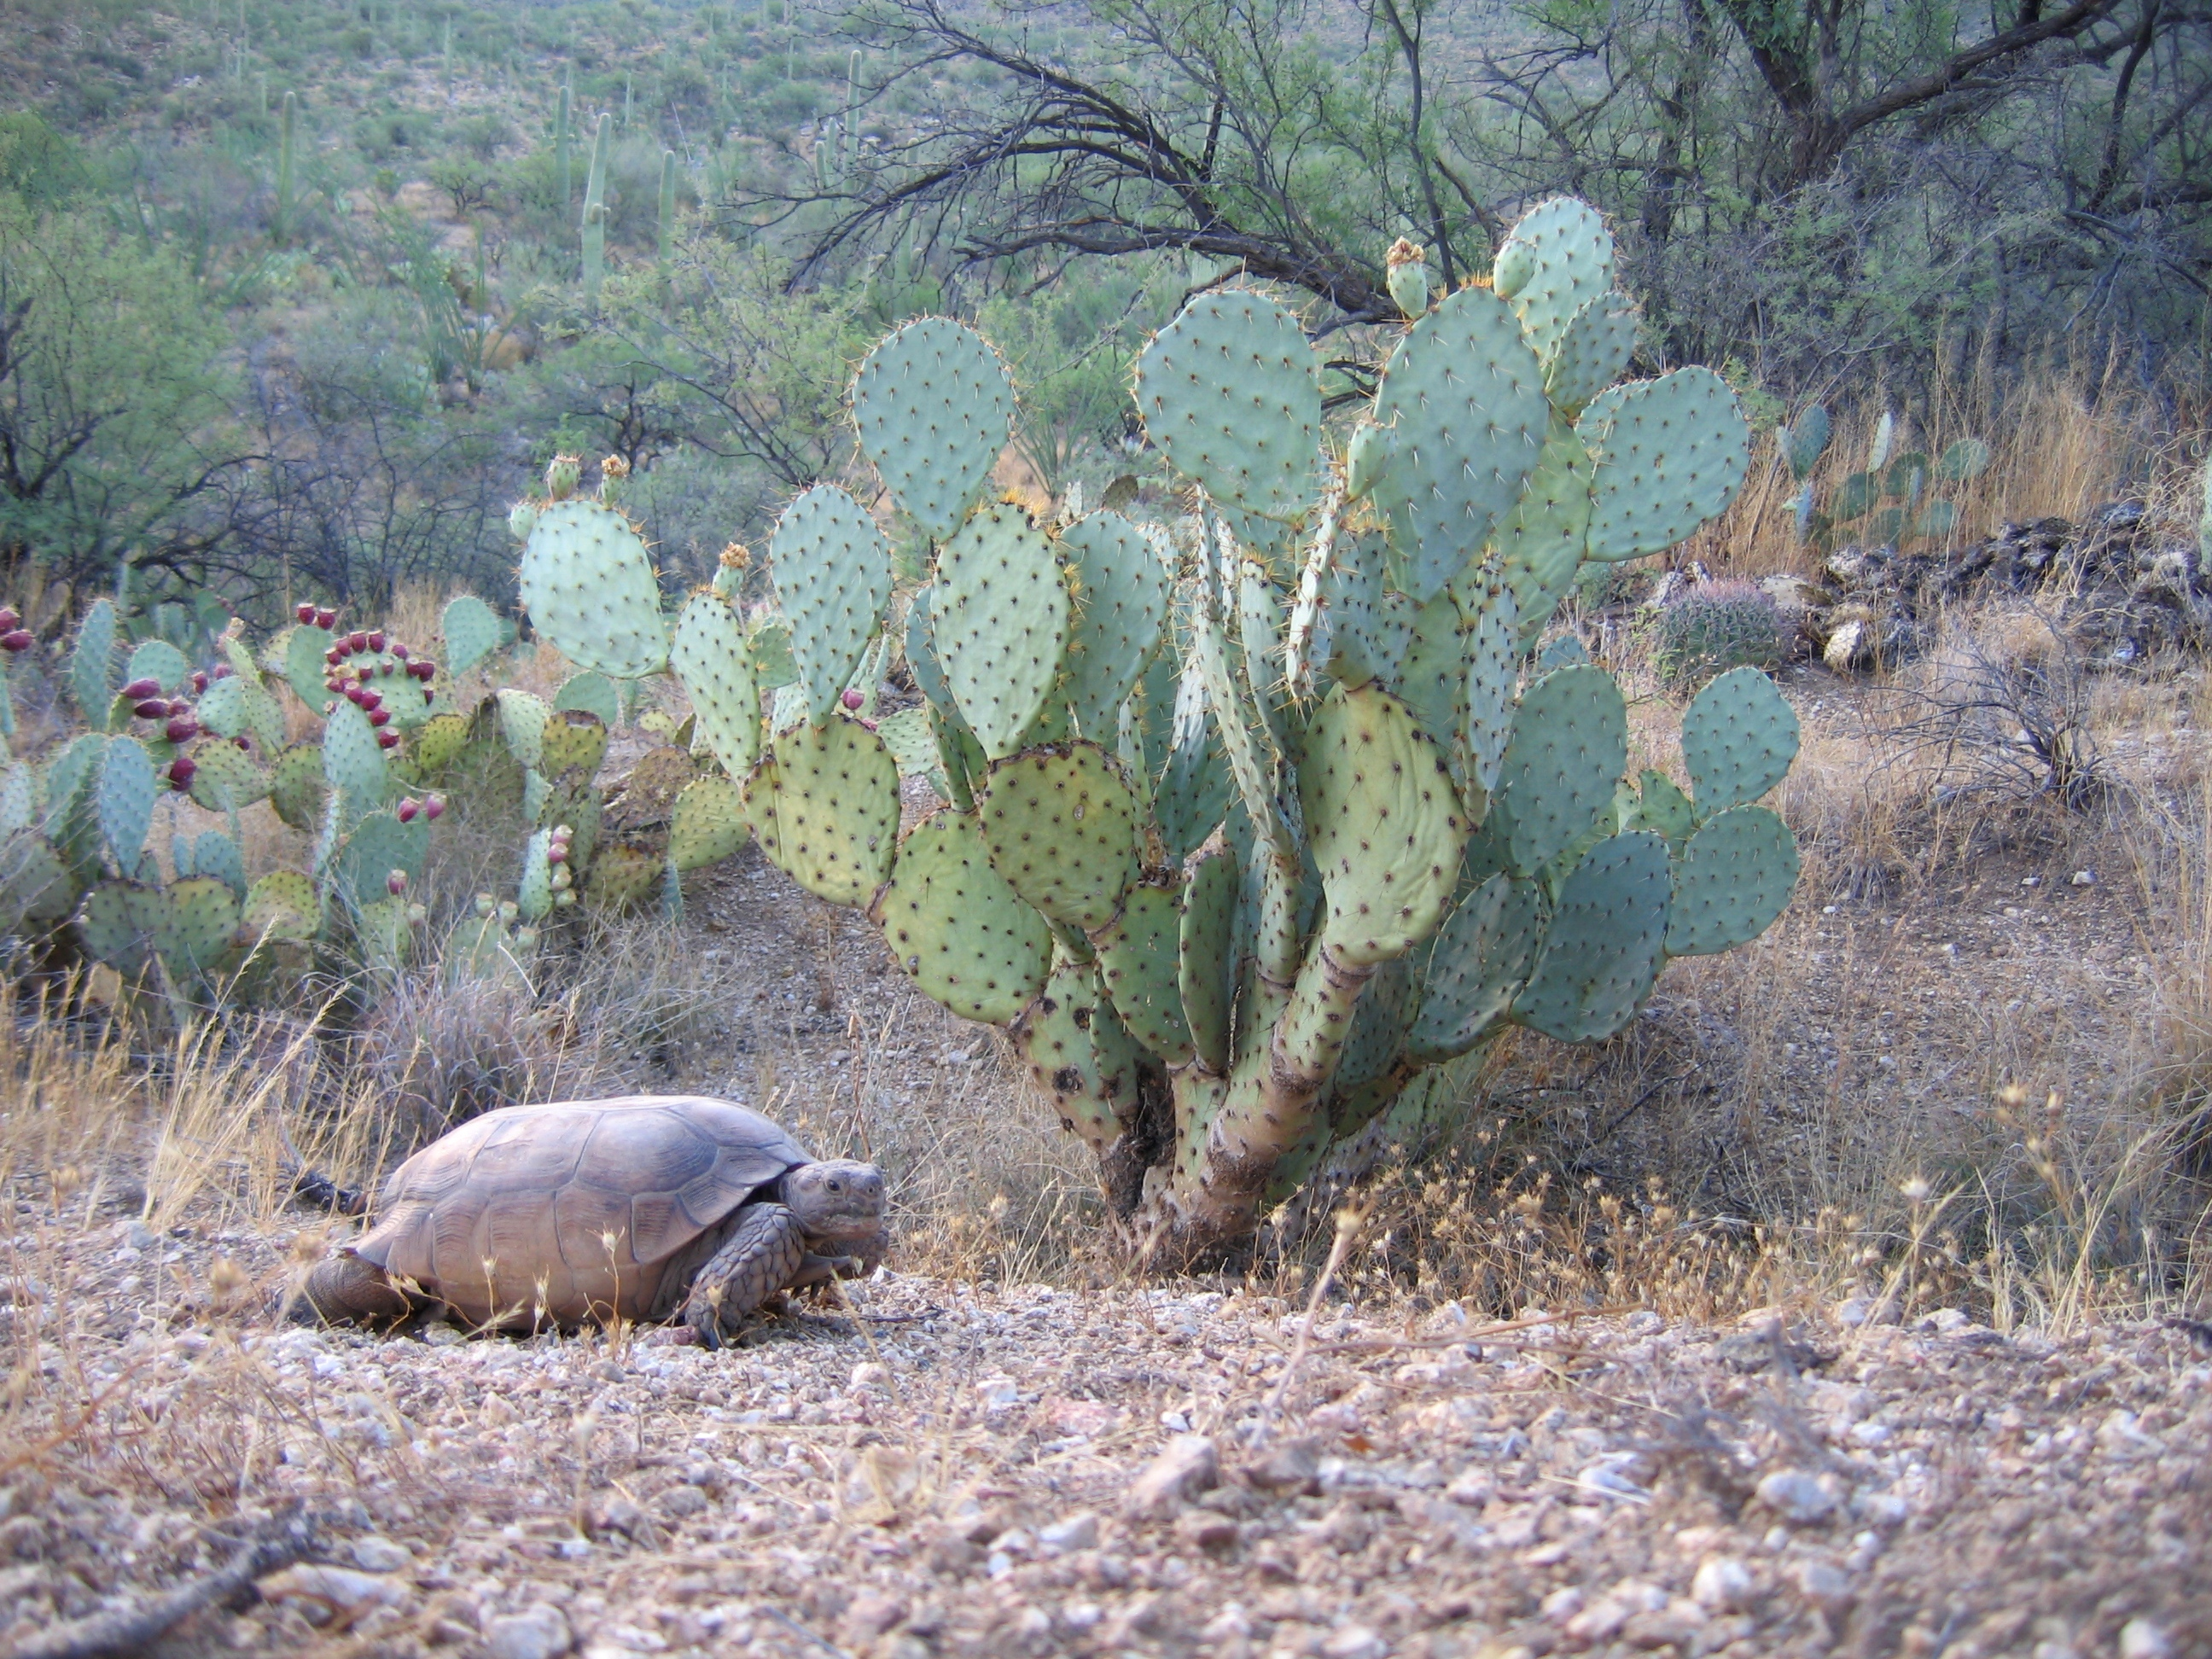
\includegraphics[height=3in,width=4in]{Ch3/figs/Erin_Zylstra_2.jpg}
\caption{Desert tortoise in its native habitat ({\it Photo credit: Erin
  Zylstra, Univ. of Arizona}.}
\label{closed.fig.tortoise}
\end{figure}

\begin{figure}
\centering
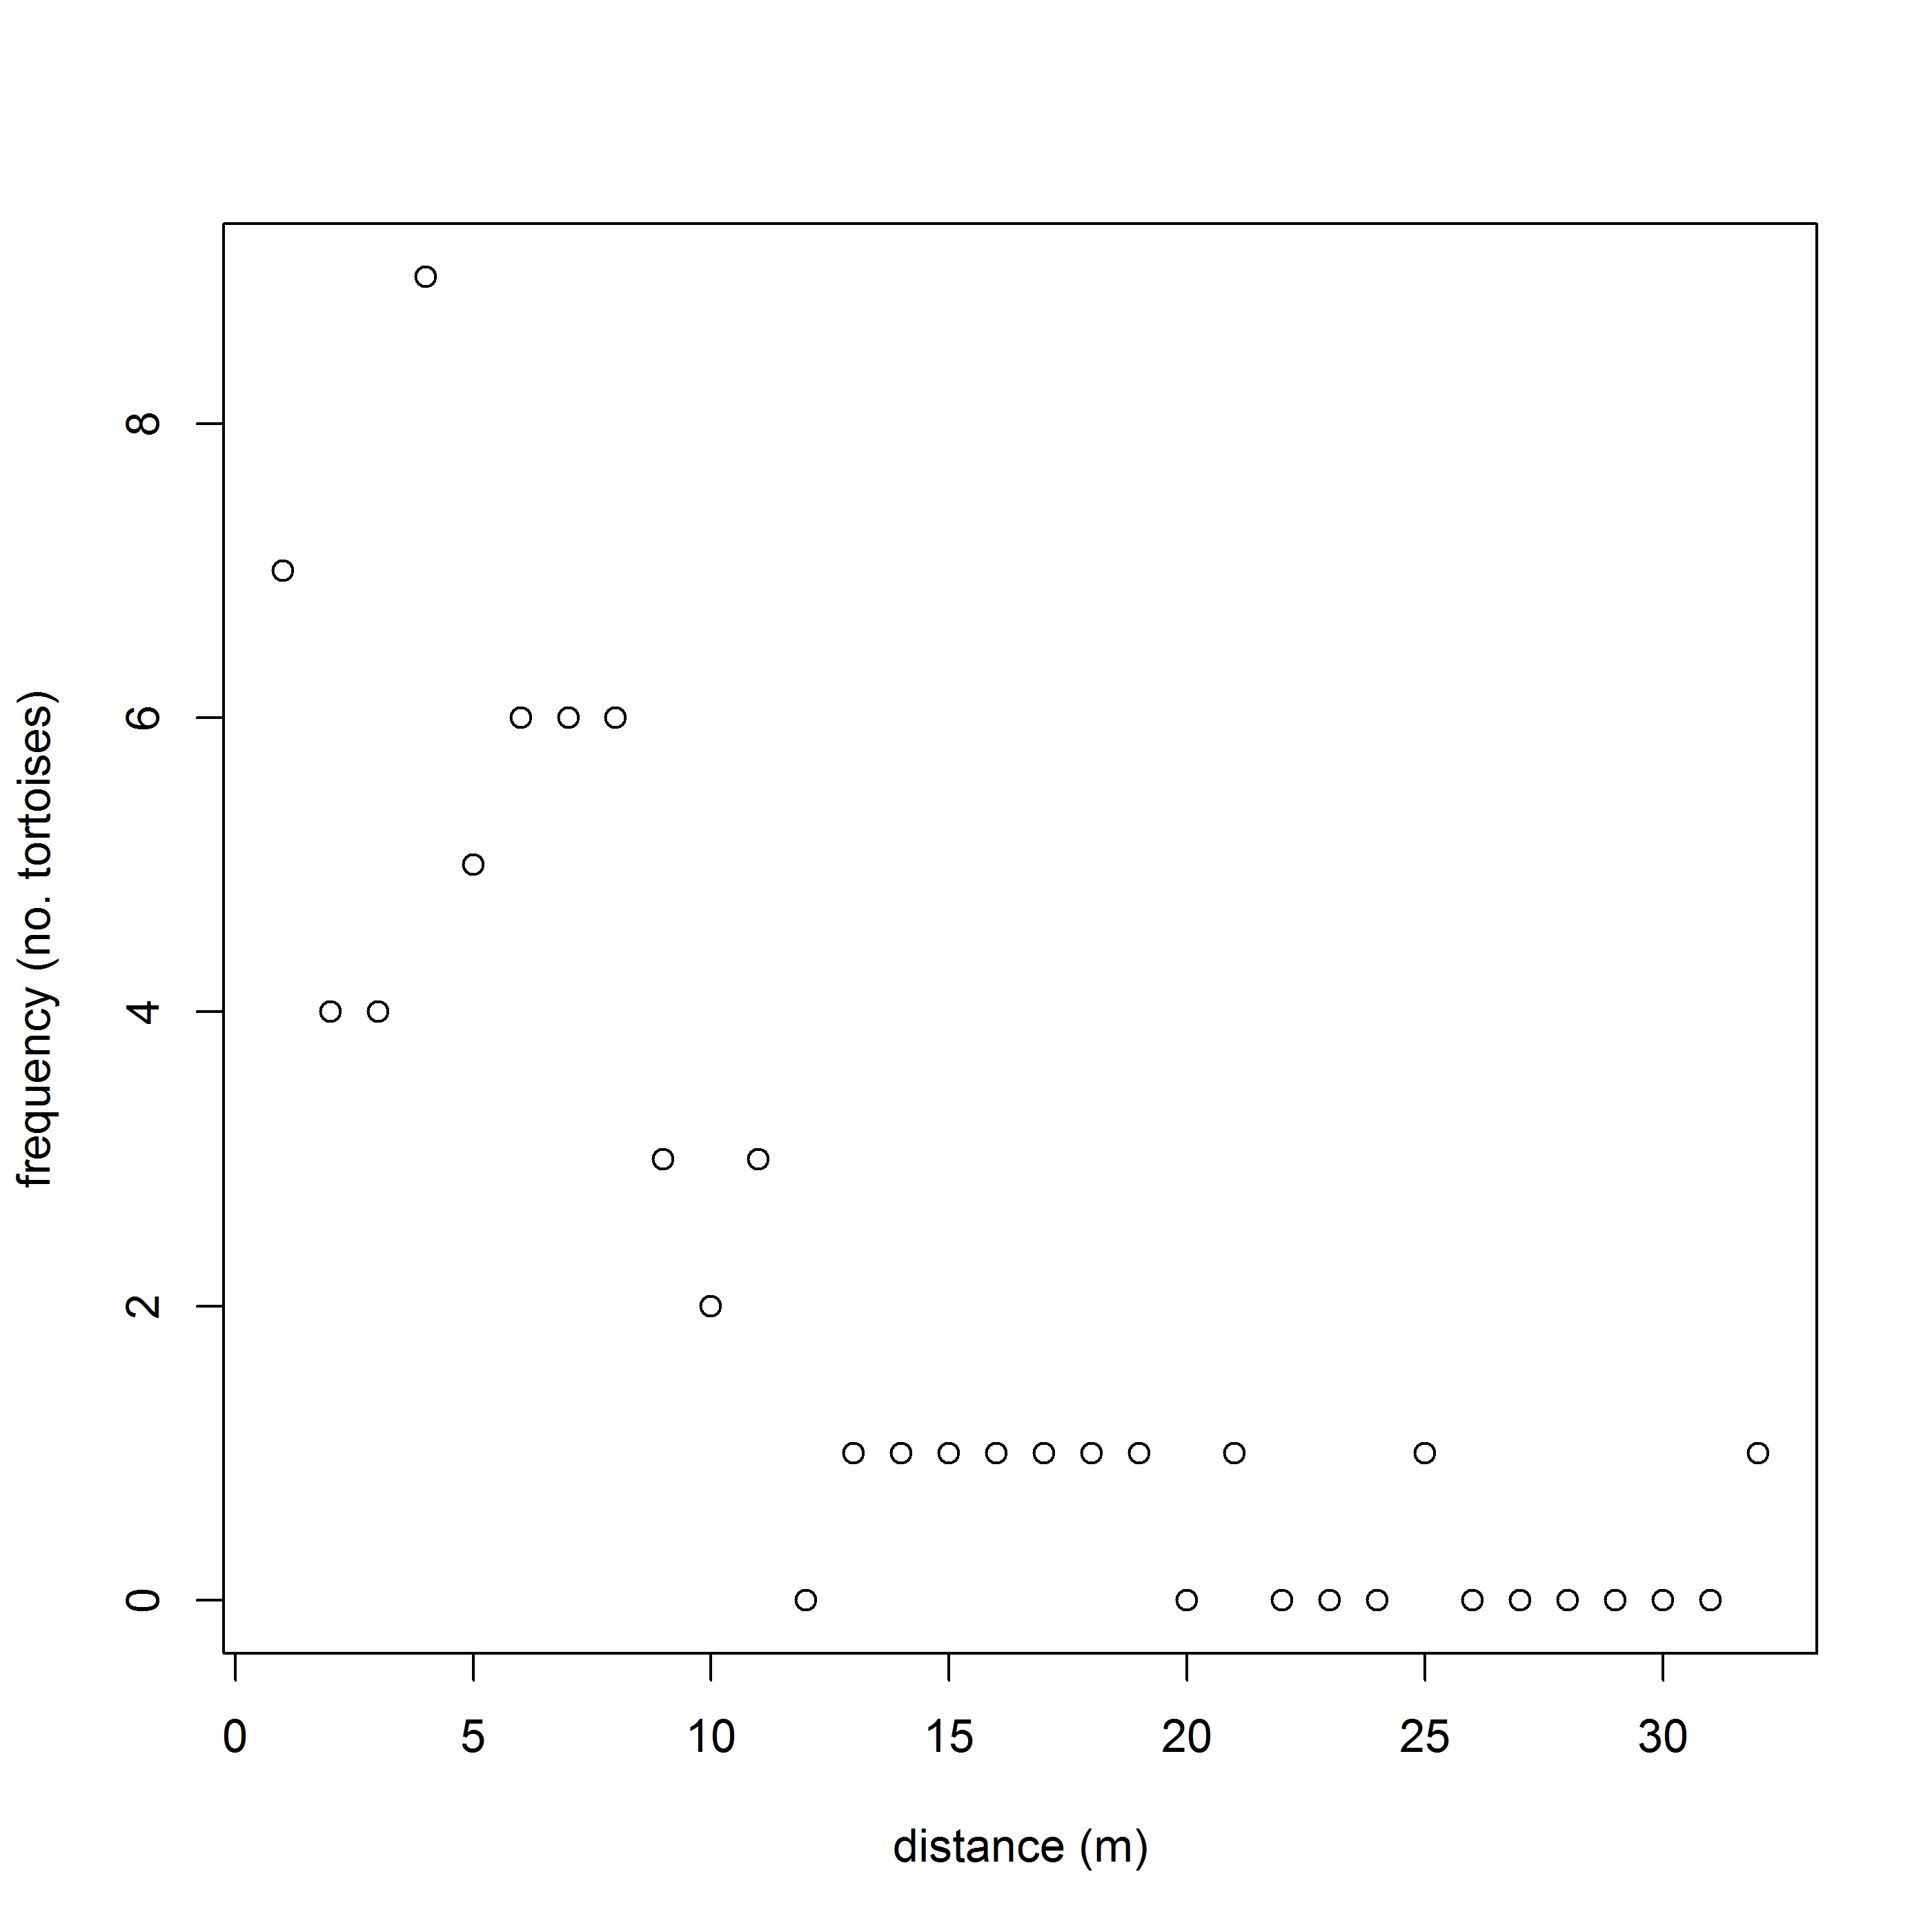
\includegraphics[height=3.35in,width=3.35in]{Ch3/figs/tortoise.png}
\caption{Histogram of Sonoran desert tortoise detections on 120 km of
transects.}
\label{closed.fig.tortoisehist}
\end{figure}

Commands
for reading in and organizing the data for analysis by {\bf WinBUGS}, followed by
writing the model to a text file, are given below. Note that the total sampled area of
the transects \mbox{\tt striparea} is input as data, and computed as:
$120$ (transects)
multiplied by the length ($1000$ m) and width ($B=40$ m), then
multiplied by 2, and then divided by $10000$ to make everything in units
of individuals {\it per} ha. The full script, provided with the
\mbox{\tt scrbook} {\bf R} package, we also give some commands for
analyzing the data using \mbox{\tt unmarked}
\citep{fiske_chandler:2011} using hierarchical distance sampling
models \citep{royle_etal:2004}.
{\small
\begin{verbatim}
data(toroise)
x<-tortoise[,"Dist"]
nind<-sum(!is.na(x))

y<-rep(1,nind)        # create encounter vector
nz<-700               # data augmentation
y<-c(y,rep(0,nz))     # add 0s to the encounter vector
x<-c(x,rep(NA,nz))    # pad distance vector with NA
z<-y                  # starting vals for data augmentation variables

cat("
model{
alpha1~dunif(0,10)
sigma<- sqrt(1/(2*alpha1))
psi~dunif(0,1)

for(i in 1:(nind+nz)){
   z[i]~dbern(psi)    # DA Variables
   x[i]~dunif(0,B)    # B=strip width
   p[i]<-exp(logp[i])   # DETECTION MODEL
   logp[i]<-   -alpha1*(x[i]*x[i])
   mu[i]<-z[i]*p[i]
   y[i]~dbern(mu[i])  # OBSERVATION MODEL
 }

N<-sum(z[1:(nind+nz)])
D<- N/striparea  # area of transects
}
",file="dsamp.txt")
\end{verbatim}
}

Next, we bundle the data,
provide initial values, indicate which parameters to monitor, and then
pass those things to {\bf WinBUGS}:
{\small
\begin{verbatim}
library("R2WinBUGS")

# density to be reported in units of ind/ha
data<-list(y=y,x=x,nz=nz,nind=nind,B=40,striparea=(120*1000*40*2/10000))
params<-list('alpha1','sigma','N','D','psi')
inits =  function() {list(z=z, psi=runif(1), alpha1=runif(1,0,.02) )}
fit = bugs(data, inits, params, model.file="dsamp.txt",working.directory=getwd(),
       debug=FALSE, n.chains=3, n.iter=3000, n.burnin=1000, n.thin=2)
\end{verbatim}
}
Posterior summaries are provided in the following summary
table. Estimated density (posterior mean) is $0.54$ individuals {\it
  per} ha and the estimated scale parameter of the distance function
(posterior mean) is $\sigma=9.12$ meters.  The Rhat statistics of
around $1.02$ suggest that slightly longer MCMC simulations might be
useful. The posterior mass of the data augmentation parameter $\psi$
is located away from the upper-bound $\psi=1$ and so the degree of
data augmentation appears sufficient.
{\small
\begin{verbatim}
> print(fit,digits=2)
Inference for Bugs model at "dsamp.txt", fit using WinBUGS,
 3 chains, each with 3000 iterations (first 1000 discarded), n.thin = 2
 n.sims = 3000 iterations saved
           mean    sd   2.5%    25%    50%    75%  97.5% Rhat n.eff
alpha1     0.01  0.00   0.00   0.01   0.01   0.01   0.01 1.02   130
sigma      9.12  0.77   7.77   8.57   9.07   9.62  10.77 1.02   130
N        516.67 54.71 415.00 478.00 516.00 552.00 632.00 1.02   100
D          0.54  0.06   0.43   0.50   0.54   0.57   0.66 1.02   100
psi        0.61  0.07   0.49   0.56   0.61   0.66   0.75 1.02    96

[.... some output deleted .... ]

\end{verbatim}
}




\begin{comment}
\subsection{Example: Muntjac deer survey from Nagarahole, India }


Here we fit distance sampling models to distance sampling data on the
muntjac deer (Muntiakus muntjak) collected in the year 2004 from
Nagarahole National Park in southern India
(Kumar et al. unpublished data). The muntjac is
a solitary species and distance measurements were made on 57 groups
that were largely singletons with 4 pairs of individuals.  Commands
for reading in and organizing the data for {\bf WinBUGS}, followed by
writing the model to a text file, are given below. Note that the total sampled area of
the transects is fed in as ``striparea'' which is $708$ (km of transect walked)
multiplied by the strip width ($B=120 = 0.12$ km) multiplied by 2.
{\small
\begin{verbatim}
library("R2WinBUGS")
data<- read.csv("Muntjac.csv")
hist(data[,3],30)
nind<-nrow(data)
y<-rep(1,nind)
nz<-400
y<-c(y,rep(0,nz))
x<-data[,3]
x<-c(x,rep(NA,nz))
z<-y

cat("
model{
beta~dunif(0,10)
psi~dunif(0,1)

for(i in 1:(nind+nz)){
   z[i]~dbern(psi)    # DA Variables
   x[i]~dunif(0,B)    # B=strip width
   p[i]<-exp(logp[i])   # DETECTION MODEL
   logp[i]<-   -beta*(x[i]*x[i])
   mu[i]<-z[i]*p[i]
   y[i]~dbern(mu[i])  # OBSERVATION MODEL
 }
N<-sum(z[1:(nind+nz)])
D<- N/striparea  # area of transects
}
",file="dsamp.txt")
\end{verbatim}
}
Next, we provide inits, indicate which parameters to monitor, and then
pass those things to {\bf WinBUGS}:
{\small
\begin{verbatim}
data<-list(y=y,x=x,nz=nz,nind=nind,B=120,striparea=(708*2*.120))
params<-list('beta','N','D','psi')
inits =  function() {list(z=z, psi=runif(1), beta=runif(1,0,.02) )}
fit = bugs(data, inits, params, model.file="dsamp.txt",working.directory=getwd(),
       debug=T, n.chains=3, n.iter=11000, n.burnin=1000, n.thin=2)
\end{verbatim}
}
Posterior summaries are provided in the following table. Estimated
density is pretty low, 1.1 individuals per sq. km.\footnote{ This is much
  lower than Samba's estimate produced from WinBUGS accounting for group
  size. Reason unknown. }
{\small
\begin{verbatim}
Inference for Bugs model at "dsamp.txt", fit using WinBUGS,
 3 chains, each with 11000 iterations (first 1000 discarded), n.thin = 2
 n.sims = 15000 iterations saved
           mean    sd   2.5%    25%    50%    75%  97.5% Rhat n.eff
beta       0.00  0.00   0.00   0.00   0.00   0.00   0.00    1  1100
N        185.73 26.53 138.00 167.00 184.00 203.00 242.00    1   570
D          1.09  0.16   0.81   0.98   1.08   1.20   1.42    1   570
psi        0.41  0.06   0.30   0.36   0.40   0.45   0.54    1   670
deviance 655.74 16.26 626.00 644.50 655.10 666.40 689.80    1  1300

xxxxxxx$Is the first line (beta) reasonable?$xxxxxxxxxx

[.... some output deleted .... ]
\end{verbatim}
}

\end{comment}























\section{Summary and Outlook}

Traditional closed population capture-recapture models are closely
related to binomial generalized linear models.  Indeed, the only real
distinction is that in capture-recapture models, the population size
parameter $N$ (corresponding also to the size of a hypothetical
``complete'' data set) is unknown.  This requires special
consideration in the analysis of capture-recapture models. The
classical approach to inference recognizes that the observations don't
have a standard binomial distribution but, rather, a truncated
binomial (from which which the so-called {\it conditional likelihood}
derives) since we only have encounter frequency data on observed
individuals. If instead we analyze the models using data augmentation,
the observations can be modeled using a zero-inflated binomial
distribution. In short, when we deal with the unknown-$N$ problem using
data augmentation then we are left with zero-inflated GLM and GLMMs
instead of ordinary GLM or GLMMs. The analysis of such zero-inflated
models is practically convenient, especially using the various
Bayesian analysis packages that use the {\bf BUGS} language.

Spatial capture-recapture models that we will consider in the rest of
the chapters of this book are closely related to what have been called
individual covariate models. Heuristically, spatial capture-recapture
models arise by defining individual covariates based on observed
locations of individuals -- we can think of using some function of
mean encounter location as an individual covariate. We did this in a
novel way, by using distance to the centroid of the trapping array as
a covariate. We analyzed the {\it full likelihood} using data
augmentation, and placed a prior distribution on the individual
covariate which was derived from an assumption that individual
locations are, a priori, uniformly distributed in space. This
assumption provides for invariance of the density estimator to the
choice of population size area (induced by maximum distance from the
centroid of the trap array). The model addressed some important problems in the
use of closed population models: it allows for heterogeneity in
encounter probability due to the spatial context of the problem and it
also provides a direct estimate of density because area is a feature
of the model (via the prior on the individual covariate). The model is
still not completely general because it does not make use of
the fully spatial encounter histories, which provide direct
information about the locations and density of individuals.  A
specific individual covariate model that is in widespread use is
classical distance sampling. The model underlying distance
sampling is precisely a special kind of SCR model - but one without
replicate samples. Understanding distance sampling and individual
covariate models more broadly provides a solid basis for understanding
and analyzing spatial capture-recapture models.



%%% TO DO  as of 12/29/11

 %%% Spell check document
 %%% ?all-zero? should be all-zero and not all zero ?all zero? ?all 0? etc..
 %%% Fix up R scripts and consolidate for R package
 %%% R commands to process wolverine data need included in that section

 %%% Run Wolverine 2k 4k and 8k grids in JAGS compare to WinBUGS
 %%%     insert those results in text

 %%%  For discrete state-space stuff, convert BUGS output to JAGS and
 %%%  figure out MC errors
 %%% Finish Table that has those results in it



\chapter{Fully Spatial Capture-Recapture Models}
\markboth{Chapter 4 }{}
\label{chapt.scr0}

\vspace{.3in}

In previous sections we discussed models that could be
viewed as primitive spatial capture-recapture models. We looked at a
basic distance sampling model and we also considered a classical
individual covariate modeling approach in which we defined a covariate
to be the distance from the (estimated) home range center to the center of
the trap array. These were spatial in the sense that they included
some characterization of where individuals live but, on the other
hand, only a primitive or no characterization of trap location.  That
said, there is only a small step from these two models to spatial
capture-recapture models that we consider in this chapter, which fully
recognize the spatial attribution of both individual animals {\it and}
the locations of encounter devices.

Fully spatial capture-recapture models must accommodate the spatial
organization of individuals and the encounter devices because the
encounter process occurs at the level of individual traps.  Failure to
consider the trap-specific data is the key deficiency
with classical ad-hoc approaches which aggregate encounter information
to the resolution of the entire trap array. We have  previously
addressed some problems that this induces including induced
heterogeneity in encounter probability, imprecise notation of ``sample
area'' and not being able to accommodate trap-specific
effects or trap-specific missing values.
In this chapter we resolve these issues by developing 
our first fully spatial capture-recapture
model which turns out to be precisely the model considered in sec. \ref{closed.sec.indcov},
 but instead of defining the individual covariate to be distance
to the centroid of the array we define $J$ individual covariates - the
distance to {\it each} trap. And, instead of using estimates of
individual locations ${\bf s}$, we consider a fully hierarchical model in
which we regard ${\bf s}$ as a latent variable and impose a prior
distribution on it.  We can think of having $J$ independent
capture-recapture studies generating one data set for each trap, and
applying the individual covariate model with random activity centers,
and that is all the basic SCR model is.

In the following sections of this chapter we investigate the basic
spatial capture-recapture model, which we refer to as ``model SCR0'',  and address some important
considerations related to its analysis in {\bf WinBUGS}. We also demonstrate
how to summarize posterior output for the purposes of producing
density maps or spatial predictions of density.

\section{Sampling Design and Data Structure}

In our development here, we will assume a standard sampling design in
which an array of $J$ traps is operated for $K$ time periods (say,
nights) producing encounters of $n$ individuals.  Because sampling
occurs by traps and also over time, the most general data structure
yields encounter histories for {\it each individual} that are
temporally {\it and} spatially indexed. Thus a typical data set will
include an encounter history {\it matrix} for each individual.  For
the most basic model, there are no time-varying covariates that
influence encounter, there are no explicit individual-specific
covariates, and there are no covariates that influence density. Hence, we will
develop models in this chapter for encounter data that are aggregated
over the temporal replicates. For example, suppose we observe 6
individuals in sampling at 4 traps over 3 nights of sampling then a
plausible data set is the $6 \times 4$ matrix of encounters, out of 3,
of the form:
\begin{verbatim}
      trap1 trap2 trap3 trap4
 [1,]     1     0     0     0
 [2,]     0     2     0     0
 [3,]     0     0     0     1
 [4,]     0     1     0     0
 [5,]     0     0     1     1
 [6,]     1     0     1     0
\end{verbatim}

We develop models in this chapter for passive detection 
devices such as ``hair snares''
or other DNA sampling methods \citep{kery_etal:2010,
  gardner_etal:2010jwm} and related types of sampling devices in which
(i) devices (effective ``traps'') may capture any number of individuals (i.e.,
they don't fill up; \begin{comment}
This is referred to as a ``multi-catch'' type of
sampling \citep{efford_etal:2009ecol})\end{comment}; (ii) an individual may be
captured in more than one trap during each occasion but (iii) 
individuals can be encountered at most 1 time by each trap during any
occasion.  Hair snares for sampling DNA from bears and other species
function according to these rules. An individual bear wandering about
its territory might come into contact with  $>1$ devices; A device may
encounter multiple bears; However, generally speaking, it will not be
possible to attribute multiple visits of the same individual to
distinct encounter events.

The statistical assumptions are that individual encounters
within and among traps are independent, and this allows us to regard
individual- and trap-specific encounters as {\it independent} Bernoulli trials
(see next section).  These basic (but admittedly at this point
somewhat imprecise) assumptions define the basic spatial
capture-recapture model, which we will refer to as ``SCR0'' 
so that we may use that model as a point of reference without having
to provide a long-winded enumeration of assumptions and sampling
design each time we do. We will make things more precise as we develop
a formal statistical definition of the model shortly.

While the model is most directly relevant
to hair snares and other DNA sampling methods for which multiple
detections of an individual are not distinguishable,
we will also make use of the model for data that arise from
camera-trapping studies. In practice, with camera trapping,
individuals might be photographed several times in a night but it is
common to 
 distill such data into a single binary encounter event for
reasons discussed later in Chapt. \ref{chapt.poisson-mn}.


\section{The binomial observation model }

If sampling devices are operated over $K$ time periods or sampling
occasions (e.g., in practice,
nights), and we assume that individual encounters are independent
across the $K$ sampling occasions, so that   
 individual and trap-specific encounters, $y_{ij}$,
are mutually independent outcomes of a binomial random variable:
\begin{equation}
	y_{ij} \sim \mbox{Bin}(K, p_{ij})
\label{scr0.eq.bin}
\end{equation}
This is the basic model underlying logistic regression (Chapt. \ref{chapt.glms})
as well as standard closed population models
(Chapt. \ref{chapt.closed}). The key
element of the model is that the encounter probability $p_{ij}$
depends 
on  both individual and trap. In a sense,
then, we can think of each {\it trap} as producing individual level
encounter history data of the classical variety - an $\mbox{\tt nind}
\times \mbox{\tt nreps}$
matrix of 0's and 1's (this is the ``encountered at most 1 time''
assumption).


As we did in sec. \ref{closed.sec.indcov}, we will make explicit the notion that
$p_{ij}$ is defined conditional on {\it where}  individual $i$
lives. Naturally, we think about defining an individual home range and
then relating $p_{ij}$ explicitly to the centroid of the individuals
home range, or its center of activity \citep{efford:2004,
  borchers_efford:2008, royle_young:2008}.  Therefore, define ${\bf
  s}_{i}$, a two-dimensional spatial coordinate, to be the activity
center for individual $i$. Then, the SCR model postulates that
encounter probability, $p_{ij}$, is a decreasing function
of distance between ${\bf s}_{i}$ and the location of trap $j$, ${\bf x}_{j}$.
 Naturally, if we think of modeling binomial counts using
logistic regression, we think about specifying the model according to:
\begin{equation}
	\mbox{logit}(p_{ij}) = \alpha_{0} + \alpha_1 ||{\bf s}_{i}-{\bf x}_{j} ||
\label{scr0.eq.logit}
\end{equation}
where, here, $||{\bf s}_{i}-{\bf x}_{j}||$ is the distance between
${\bf s}_{i}$ and ${\bf x}_{j}$. We sometimes write $||{\bf
  s}_{i}-{\bf x}_{j}|| = dist({\bf s}_{i},{\bf x}_{j}) =
d_{ij}$. Alternatively, if we think about distance sampling then we
might use the a model of the form:
\[
p_{ij} = p_{0}*\exp(-\alpha_{1} *||{\bf s}_{i}-{\bf x}_{j}||^2)
\]
which is usually referred to as the ``half-normal'' model in distance
sampling literature. Because it is the kernel of a bivariate normal or
Gaussian probability
density function we will refer to it as the ``(bivariate) normal'' or
``Gaussian'' model. 
There are a large number of standard detection models 
commonly used, and we consider these in
Chapt. \ref{chapt.covariates}).
Note that the bivariate normal model is equivalently represented as 
\begin{equation}
\log(p_{ij})  = \log(p_{0}) - \alpha_{1} *||{\bf s}_{i}-{\bf x}_{j}||^2
\label{scr0.eq.norm}
\end{equation}
which we make use of sometimes in specifying the model in the \bugs language. 
%We would always like to be clear that encounter probability depends on individual activity
%centers {\it and} trap locations {\it and} parameter(s) $\theta$, and
%so it would be ideal to write $p({\bf s}_{i},{\bf x}_{j}; \theta)$ or
%something similar. However, this can be extremely unwieldy and
%clutter up what are otherwise extremely simple mathematical
%expressions and formulae. As such, we will usually abbreviate these
%various dependencies by writing $p_{ij}$ or sometimes $p_{\theta,ij}$,
%understanding that $p_{ij}$ is actually a function of the various important
%quantities.
We probably expect that the parameter $\alpha_{1}$ in
Eq. \ref{scr0.eq.logit} or \ref{scr0.eq.norm} should be negative, so
that the probability of encounter decreases with distance between the
trap and individual home range center.  
Whatever model we choose for encounter probability, we should always keep
in mind that the model is described conditional on ${\bf s}_{i}$,
which is an unobserved random variable.  Thus, to be precise about
this, we should write the observation model as
\[
y_{ij}|{\bf s}_{i} \sim \mbox{Bin}(K, p({\bf s}_{ij};\alpha_{1}))
\]


The joint likelihood for the
data, conditional on the collection of individual activity centers,
can therefore be expressed as
\[
{\cal L}(\alpha_{1} | \{ {\bf y}_{i},{\bf s}_{i} \}_{i=1}^{N})
 =  \prod_{i} \prod_{j} \mbox{Bin}(y_{ij}|p_{ij}(\alpha_{1}))
\]
If we switch the indices on the product operators, we recognize that SCR likelihood (conditional on ${\bf s}$) is the product of $J$
{\it independent} capture-recapture likelihoods - one for each trap.
However, the data have a distinct ``repeated measures'' type of structure, with
each of the $j$ likelihood contributions for each individual being
grouped by individual. Thus, we cannot analyze the model
meaningfully by $J$ trap-specific models. In classical repeated measures
types of models, we accommodate the group structure of the data using
random effects (random individual or group level variables). For SCR
models we take the same basic approach, which we develop subsequently.

\subsection{Distance as a latent variable}

If we knew precisely every ${\bf s}_{i}$ in the population (and population size $N$), then the model specified by eqs. \ref{scr0.eq.bin} and
\ref{scr0.eq.logit} would be just an ordinary logistic
regression-type of a model which we learned how to fit using
\winbugs
 previously (Chapt. \ref{chapt.glms}), with a covariate $d_{ij}$. However,
the activity centers are unobservable even in the best possible
circumstances. In that case, $d_{ij}$ is an unobserved variable,
as in classical random effects models. We need to therefore
extend the model to accommodate these random variables with an
additional model component. A standard, and perhaps not unreasonable,
assumption is the so-called ``uniformity assumption'' which is to say
that the ${\bf s}_{i}$ are uniformly distributed over space (the
obvious next question ``which space?'' is addressed below).  This
uniformity assumption amounts to a uniform prior distribution on ${\bf
  s}_{i}$, i.e., the pdf of ${\bf s}_{i}$ is constant, which we may
express
\begin{equation}
	\Pr({\bf s}_{i}) \propto \mbox{\tt const}
\label{scr0.eq.sprior}
\end{equation}
 As it turns out, this assumption is usually not precise
enough to fit SCR models in practice for reasons we discuss in the
following section.  We will give another way to represent this prior
distribution that is more concrete, but depends on specifying the
``state-space'' of the random variable ${\bf s}_{i}$. The term
state-space is a technical way of saying ``the space of all possible outcomes''.

To summarize the preceeding model developing, a basic SCR model is
defined by 3 essential components:
\begin{itemize}
\item[(1)] Observation model: $y_{ij}|{\bf s}_{i} \sim \mbox{Bin}(K, p_{ij})$
\item[(2)] Encounter probability model: $\mbox{logit}(p_{ij}) = \alpha_{0} +
  \alpha_{1}*||{\bf s}_{i}-{\bf x}_{j}||$
\item[(3)] Point process model: $\Pr({\bf s}_{i} ) \propto \mbox{\tt const}$
\end{itemize}
Therefore, the SCR model is little more than an ordinary
capture-recapture model for closed populations. It is such a model,
but augmented with a set of ``individual effects'', ${\bf s}_{i}$,
which relate some sense of individual location to encounter
probability. 

\section{ The Binomial Point-process Model}

The collection of individual activity centers ${\bf s}_{1},\ldots,
{\bf s}_{N}$ represents a realization of a {\it binomial point process}
\citep[][p. xyz]{illian_etal:2008}.  The binomial point process (BPP)
is analogous to a Poisson point process in the sense that it
represents a ``random scatter'' of points in space - except that the
total number of points is {\it fixed}, whereas, in a Poisson point
process, it is random (having a Poisson distribution).  As an example,
we show in Fig. \ref{scr0.fig.bpp} locations of 20 individual activity
centers (black dots) in relation to a grid of 25 traps. For a Poisson
point process the number of such points in the prescribed state-space
would be random whereas often we will simulate fixed numbers of
points, e.g., for evaluating the performance of procedures such as how
well does our estimator perform of $N=50$?
\begin{figure}
\begin{center}
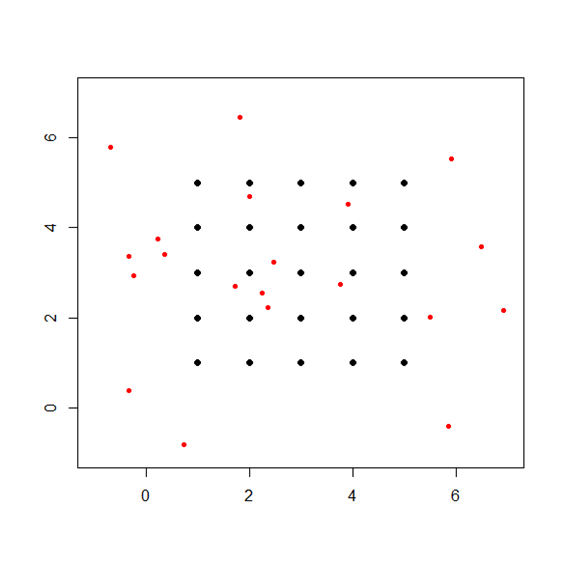
\includegraphics[height=2.5in]{Ch4/figs/binomialpoint}
\end{center}
\caption{Realization (small dots) of a binomial point process with $N=20$. The
  large dots represent trap locations.}
\label{scr0.fig.bpp}
\end{figure}

It is natural to consider a binomial point process in the context of
capture-recapture models because it preserves $N$ in the model and thus
preserves the linkage directly with closed population models. In fact,
under the binomial point process model, model $M_0$ and other closed
models are simple limiting cases of SCR models, i.e., as the
coefficient on distance ($\alpha_1$ above) tends to 0.
In addition, use of
the BPP model allows us to use data augmentation for Bayesian analysis
of the models as in Chapt. \ref{chapt.closed}, thus yielding a methodologically
coherent approach to analyzing the different classes of
models. Despite this, making explicit assumptions about $N$, such as
Poisson, is convenient in some cases (see Chapt. \ref{chapt.hscr}).

One consequence of having fixed $N$, in the BPP model, is that the
model is not strictly a model of ``complete spatial randomness''. This
is because if one forms counts $n(A_{1}),\ldots, n(A_{k})$ in any set
of disjoint regions say $A_{1}, \ldots, A_{k}$, then these counts are
{\it not} independent.  In fact, they have a multinomial distribution
\citep[see][p. 61]{illian_etal:2008}. Thus, the BPP model introduces
a slight bit of dependence in the distribution of points. However, in
most situations this will have no practical effect on any inference or
analysis and, as a practical matter, we will usually regard the BPP
model as one of spatial independence among individual activity centers
because each activity center is distributed independently of each
other activity center. Despite this implicit independence we see in
Fig. \ref{scr0.fig.bpp} that {\it realizations} of randomly distributed
points will typically exhibit distinct non-uniformity. Thus,
independent, uniformly distributed points will almost never appear
regularly, uniformly or systematically distributed. For this reason,
the basic binomial (or Poisson) point process models are enormously
useful in practical settings.  More relevant for SCR models is that we
actually have a little bit of data for some individuals and thus the
resulting posterior point pattern can deviate strongly from
uniformity, a point we come back to repeatedly in this book.
The uniformity hypothesis is only
a {\it prior} distribution which is directly affected by the quantity
and quality of the observed data, to produce a posterior distribution which
may appear distinctly non-uniform.


\subsection{Definition of home range center}

Some will be offended by our use of the concept of ``home range
center'' and question whether such notions as home ranges are useful
for some (or perhaps {\it any}) particular species.  Indeed, the idea
of a home range is a vague and purely phenomenological construct
anyway.  Despite this, it doesn't really matter whether or not a home
range makes sense for a particular species - individuals of any
species inhabit {\it some} region of space and we can define the
``home range center'' to be the center of the space that individual
was occupying (or using) during the period in which traps were
active. Thinking about it in that way, it could even be observable
(almost) as the centroid of a very large number of radio fixes over
the course of a survey period or a season.  Thus, this practical
version of a home range center in terms of space usage is a
well-defined construct regardless of whether one thinks the home range
itself is a meaningful concept, even if individuals are not
particularly territorial.  This is why we usually use the term
``activity center'' and we recognize that this is a transient thing
which applies only to a well-defined period of study.
%See sec. \ref{sec.scr0.implied} for more discussion of how to 
%interpret ${\bf s}$ in the context of the detection probability
%model. 


\subsection{The state-space of the point process}

Shortly we will focus on Bayesian analysis of this model with $N$
known so that we can directly apply to this situation what we learned
in Chapt. \ref{chapt.glms}. To do this, we note that the individual
effects ${\bf s}_{i},\ldots, {\bf s}_{N}$ are unknown quantities and
we will need to be able to simulate each ${\bf s}_{i}$ in the
population from the posterior distribution.  It should be self-evident
that we cannot simulate the ${\bf s}_{i}$ unless we describe precisely
the region over which they are uniformly distributed. This is the
quantity referred to above as the state-space, denoted henceforth by
${\cal S}$, which is a region or a set of points comprising the
potential values of ${\bf s}_{i}$. Thus, an equivalent explicit
statement of the ``uniformity assumption'' is
\[
{\bf s}_{i} \sim \mbox{Unif}({\cal S})
\]
where ${\cal S}$ is a precisely defined region. e.g., in Fig. 
\ref{scr0.fig.bpp}, ${\cal S}$ is the square defined by $[-1,7] \times
[-1, 7]$. Thus each of the $N=20$ points were generated by randomly
selecting each coordinate on the line $[-1, 7]$. 


\subsubsection{Prescribing the state-space}

Evidently, we need to define the state-space, ${\cal S}$. How can we
possibly do this objectively? Prescribing any particular ${\cal S}$
seems like the equivalent of specifying a ``buffer'' which we
criticized previously as being ad hoc. How is it, then, that the choice of a
state-space is {\it not} ad hoc? As a practical matter, it turns out
that estimates of density are insensitive to choice of the
state-space. As we observed in Chapt. \ref{chapt.closed}, it is true that $N$ increases
with ${\cal S}$, but only at the same rate as the area of ${\cal S}$
increases under the
prior assumption of constant density. As a result, we say that density
is invariant to ${\cal S}$ as long as ${\cal S}$ is sufficiently
large. Thus, while choice of ${\cal S}$ is (or can be) essentially
arbitrary, once ${\cal S}$ is chosen, it defines the population being
exposed to sampling, which scales appropriately with the size of the
state-space.

For our simulated system developed previously in this chapter, we
defined the state-space to be a square within which our trap array was
centered. For many practical situations this might be an
acceptable approach to defining the state-space. We provide an example
of this in sec. \ref{scr0.sec.wolverine} below in which the trap array is
irregular and also situated within a realistic landscape that is
distinctly irregular.  In general, it is most practical to define the
state-space as a regular polygon (e.g., rectangle) containing the trap
array without differentiating unsuitable habitat. Although defining
the state-space to be a regular polygon has computational advantages
(e.g., we can implement this more efficiently in {\bf WinBUGS} and
cannot for irregular polygons), a regular polygon induces an apparent
problem of admitting into the state-space regions that are distinctly
non-habitat (e.g., oceans, large lakes, ice fields, etc.).  It is
difficult to describe complex sets in mathematical terms that can be
used in {\bf BUGS}. As an alternative, we can provide a
representation of the state-space as a discrete set of points (sec.
\ref{scr0.sec.discrete}), that will allow specific points to be deleted
or not depending on whether they represent habitat, or we can define
the state-space as an arbitrary  collection of polygons stored as a GIS
shapefile
which can be analyzed easily using MCMC
(see sec. \ref{mcmc.sec.state-space}), but not so easily in the {\bf
  BUGS} variants.  In what follows below we provide an
analysis of the camera data defining the state-space to be a regular
continuous polygon (a rectangle).


\subsection{Invariance and the state-space as a model assumption}
\label{scr0.sec.invariance}

We will assert for all models we consider in this book that density is
invariant to the size and extent of ${\cal S}$, if ${\cal S}$ is
sufficiently large, and as long 
as our model relating $p_{ij}$ to ${\bf  s}_{i}$ is a decreasing
function of distance.  
We can prove this easily by drawing an analogy with a 1-d case
involving 
 distance sampling.  Let $y_{j}$ be the number of individuals
captured in some interval $[d_{j-1},d_{j})$, and define $d_{J} = B$
for some large value of $B$.  
The observations from a survey are $y_{1},\ldots,y_J$ and the
likelihood is a multinomial likelihood, so the log-likelihood is of
the form
\[
logL(\{ y_{j} \}) = \sum_{j} y_{j=1}^{J} \pi_{j}
\]
where $\pi_{j}$ is the probability of detecting an individual in
distance class $j$, which depends on parameters of the detection
function (the manner of which is not relevant for the present
discussion).  For $B$ sufficiently large, we guarantee that $E[y_{J}]
= 0$ and therefore the observed frequency in the ``last cell''
contributes nothing to the likelihood, in regular situations in which
the detection function decays monotonically with distance and prior
density is constant.


Sometimes
our estimate of density can be affected by choosing ${\cal S}$ too
small. However, 
this might be sensible if ${\cal S}$ is naturally well-defined. As we discussed
in Chapt. \ref{chapt.intro}, {\bf choice of ${\cal S}$ is part of the
  model}, and thus it is sensible 
that estimates of density might be sensitive to its definition
  in problems where it is natural to restrict ${\cal S}$.
One could imagine,
however, that in specific cases where you're studying a small
population with well-defined habitat preferences, that a problem could
arise because changing the state-space around based on differing
opinions and GIS layers might have substantial changes on the density
estimates and hence those of 
population size. But this is a real biological problem and a natural
consequence of the spatial formalization of capture-recapture models -
a feature, not a bug or some statistical artifact - and it should be
resolved with better information, research, and thinking.
 For situations where there is not a natural
choice of ${\cal S}$, we should default to choosing ${\cal S}$ to be very large in order
to achieve invariance or, otherwise, evaluate sensitivity of density
estimates by trying a couple of different choices of ${\cal S}$. This is a
standard ``sensitivity to prior'' argument that Bayesians always have
to be conscious of.  We demonstrate this in our analysis of section
\ref{scr0.sec.wolverine}
below. As an additional practical 
consideration, we note that $area({\cal S})$ affects data augmentation. If you
increase $area({\cal S})$ then there are more individuals to account for and
therefore the size of the augmented data set $M$ must increase.

We have been told that one can carry-out non-Bayesian analyses of SCR
models without having to specify the state-space of the point process
or perhaps while only specifying it imprecisely.  This assertion is
incorrect. We assume people are thinking this because {\it they} don't
have to specify it explicitly because someone else has done it for
them in a package that does integrated likelihood. Even to do
integrated likelihood (see Chapt. \ref{chapt.mle}) we have to integrate the
conditional-on-${\bf s}$ likelihood over some 2-dimensional space.  It might
work that the integration can be done from $-\infty$ to $+\infty$ but
that is a mathematical artifact of specific detection functions, and
an implicit definition of a state-space that doesn't make biological
sense in any real context. %%%, even though it may in fact be innocuous.


\subsection{Connection to Model  $M_h$}  \label{scr0.sec.scrmh}

SCR models are closely related to heterogeneity models. In SCR models,
heterogeneity in encounter probability is induced by both the effect
of distance in the model for detection probability and also from
specification of the state-space. Hence, the state-space  is an
explicit element of the model. 
To understand this, suppose we have a random
effect with some prior distribution:
\[
{\bf s} \sim \mbox{Unif}({\cal S})
\]
and encounter probability is a function of ${\bf s}$, denoted by 
 $p({\bf s}) = p(y=1|{\bf s})$. 
For example, under Eq. \ref{scr0.eq.logit}
we have that 
\[
p({\bf s}) = logit^{-1} ( \alpha_{0} + \alpha_1 ||{\bf
  s}_{i}-{\bf x}_{j} || )
\]
and we can work out, either analytically or empirically, what is the
implied distribution of $p$ for a population of individuals.  We show
an illustration in Fig. \ref{scr0.fig.buffereffect} which shows a
histogram of $p$ for a hypothetical population of 100000 individuals
on a state-space enclosing our $5 \times 5$ trap array above, under
the logistic model for distance given by Eq. \ref{scr0.eq.logit}. {\bf
  R} code is provided in the {\bf R} package \mbox{\tt scrbook} to
produce this analysis for the logistic and half-normal models. The
histogram shows the encounter probability under buffers of 0.2, 0.5
and 1.0. We see the mass shifts to the left as the buffer increases,
implying more individuals with lower encounter probabilities, as their
home range centers increase in distance from the trap array.


\begin{figure}
\begin{center}
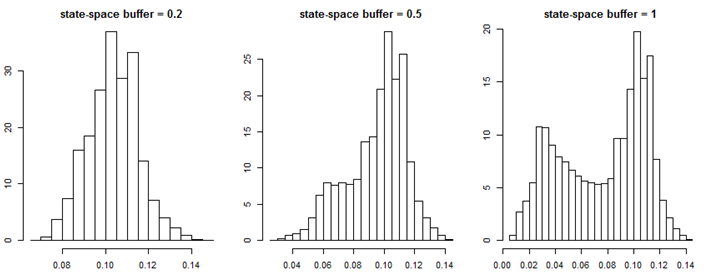
\includegraphics[width=5in]{Ch4/figs/buffereffect}
\end{center}
\caption{Implied population distribution of $p_{i}$ for a population
  of individuals as a function of the size of the state-space buffer
  around a trap array. The trap array is fixed and centered within a
  square state-space.}
xxxxxxxxxxxxxxx
$The main titles of the three panel plots are too small. I would rather call them (a), (b) and (c) and then give their associated information in the figure legend. Also, numbers on axes are very small for the sight of men in our age$ xxxxxxxxxxxxxxxxxxxx
\label{scr0.fig.buffereffect}
\end{figure}

Another way to understand this is by representing ${\cal S}$ as a set
of discrete points on a grid. In the coarsest possible case where
${\cal S}$ is a single arbitrary point, then every individual has
exactly the same $p$. As we increase the number of points in ${\cal
  S}$,  more distinct values of $p$ are possible. As such, when
${\cal S}$ is characterized by discrete points then SCR models are
precisely a type of finite-mixture model \citep{norris_pollock:1996,
  pledger:2000}, except, in the case of SCR models, we have some information about which
group an individual belong (i.e., where their activity center is), as
a result of their captures in traps.

This context suggests the problem raised by \citet{link:2003}. He
showed that in most practical situations $N$ may not be identifiable
across classes of mixture distributions which in the context of SCR
models is the pair $(g, {\cal S})$.  The difference, however, is that
we do obtain some direct information about ${\bf s}$ in SCR models and
therefore it may be reasonable to expect that
$N$ is identifiable across models characterized by $(g,{\cal
  S})$.

\subsection{Connection to Distance Sampling}

It is worth re-emphasizing that the basic SCR model is a binomial
encounter model in which distance is a covariate. As such, it is
strikingly similar to a classical distance sampling model \citep{buckland_etal:2002}. Both have
distance as a covariate but in classical distance sampling problems
the focus is on the distance between the observer and the animal at an
instant in time, not the distance between a trap and an animal's home
range center. As a practical matter, in distance sampling, ``distance'' is {\it
  observed} for those individuals that appear in the
sample. Conversely, in SCR problems, it is only imperfectly observed
(we have partial information in the form of trap observations).
Clearly, it is preferable to observe distance if possible, but 
distance sampling requires field methods that
are often not practical in many situations, e.g. when studying
carnivores such as bears or large cats. Furthermore, SCR models allow us to relax many of the
assumptions made in classical distance sampling, such as perfect detection at distance zero, and SCR models allow
for estimates of quantities other than density, such as home range
size, and space usage (see Chapts. XXXXX And \ref{chapt.ecoldist}).


\section{Simulating SCR Data}

It is always useful to simulate data because it allows you to
understand the system that you're modeling and also calibrate your
understanding with the parameter values of the model. That is, you can
simulate data using different parameter values until you obtain data
that ``look right'' based on your knowledge of the specific situation
that you're interested in. Here we provide a simple script to
illustrate how to simulate spatial encounter history data. In this
exercise we simulate data for 100 individuals and a 25 trap array laid
out in a $5 \times 5$ grid of unit spacing.  The specific encounter model is
the half-normal model given above and we used this code to simulate
data used in subsequent analyses.  The 100 activity centers were
simulated on a state-space defined by a $8 \times 8$ square within which the
trap array was centered (thus the trap array is buffered by 2
units). Therefore, the density of individuals in this system is fixed
at $100/64$.

{\small
xxxxxx$This is an example of a panel I like: The code is nicely laid out and well explained$xxxxxx
\begin{verbatim}
	set.seed(2013)
# create 5 x 5 grid of trap locations with unit spacing
traplocs<- cbind(sort(rep(1:5,5)),rep(1:5,5))
Dmat<-e2dist(traplocs,traplocs) 
ntraps<-nrow(traplocs)

# define state-space of point process. (i.e., where animals live).
# "delta" just adds a fixed buffer to the outer extent of the traps.
delta<-2
Xl<-min(traplocs[,1] - delta)
Xu<-max(traplocs[,1] + delta)
Yl<-min(traplocs[,2] - delta)
Yu<-max(traplocs[,2] + delta)

N<-100   # population size
K<- 20    # number nights of effort

sx<-runif(N,Xl,Xu)    # simulate activity centers
sy<-runif(N,Yl,Yu)
S<-cbind(sx,sy)
D<- e2dist(S,traplocs)  # distance of each individual from each trap

alpha0<- -2.5      # define parameters of encounter probability
sigma<- 0.5        #
alpha1<- 1/(2*sigma*sigma)
probcap<- plogis(-2.5)*exp( - alpha1*D*D)    # probability of encounter 
# now generate the encounters of every individual in every trap
Y<-matrix(NA,nrow=N,ncol=ntraps)
for(i in 1:nrow(Y)){
   Y[i,]<-rbinom(ntraps,K,probcap[i,])
}
\end{verbatim}
}

We remind the reader that, in presenting \R or other code snippets
throughout the book, we will deviate from our standard variable
expressions for some quantities. 
In particular, we sometimes 
substitute words for integer variable designations:
\mbox{\tt nind} (for $n$), \mbox{\tt ntraps} (for $J$), and \mbox{\tt
 nperiods} (for $K$). In our opinion this leaves less to be infereed
 in a \bugs model definition.

Subsequently we will generate data using this code packaged in an {\bf
  R}
function called \mbox{\tt simSCR0.fn} in the package \mbox{\tt
  scrbook} which takes a number of
arguments including \mbox{\tt discard0} which, if \mbox{\tt TRUE}, will return
only the encounter histories for captured individuals.  A second
argument is \mbox{\tt array3d} which, if \mbox{\tt TRUE}, returns the 3-d
encounter history array instead of the aggregated \mbox{\tt nind}
$\times \mbox{\tt ntraps}$ encounter frequencies (see below). Finally
we provide a random number seed, \mbox{\tt sd = 2013} to ensure
repeatability of the analysis here. We obtain a data set as above using the
following command:
\begin{verbatim}
data<-simSCR0.fn(discard0=TRUE,array3d=FALSE,sd=2013)
\end{verbatim}
The {\bf R} object \mbox{\tt data} is a list, so let's take a look at
what's in the list and then harvest some of its elements for further
analysis below.
{\small
\begin{verbatim}
> names(data)
[1] "Y"        "traplocs" "xlim"     "ylim"     "N"        "alpha0"   "beta"
[8] "sigma"    "K"
> Y<-data$Y
> traplocs<-data$traplocs
\end{verbatim}
}

\subsection{Formatting and manipulating real data sets}
\label{scr0.sec.formats}

Conventional capture-recapture data are easily stored and manipulated
as a 2-dimensional array, an $\mbox{\tt nind} \times \mbox{\tt
  nperiod}$ matrix, which is maximally informative for any
conventional capture-recapture model, but not for spatial
capture-recapture models.  For SCR models we must preserve the spatial
information in the encounter history information. We will routinely
analyze data from 3 standard formats:
\begin{itemize}
\item[(1)] The basic 2-dimensional data format, which is an \mbox{\tt
    nind} $\times$ \mbox{\tt ntraps} encounter frequency matrix such
  as that simulated previously. These are the total number of encounters in each
  trap, summed over replicate samples.
\item[(2)] The maximally informative 3-dimensional array, for which we
  establish here the convention that it has dimensions \mbox{\tt nind}
  $\times$ \mbox{\tt nperiods} $\times$ \mbox{\tt ntraps}.\item[(3)] We use a compact format - the ``SCR flat format'' - which
  we describe below in section \ref{scr0.sec.wolverine}.
\end{itemize}
To simulate data in the most informative format - the ``3-d array'' -
we can use the {\bf R} commands given previously but replace the last
4 lines with the following:
{\small
\begin{verbatim}
Y<-array(NA,dim=c(N,K,ntraps))
for(i in 1:nrow(Y)){
for(j in 1:ntraps){
 Y[i,1:K,j]<-rbinom(K,1,probcap[i,j])
}
}
\end{verbatim}
}
We see that a collection of $K$ binary encounter events are generated
for {\it each} individual and for {\it each} trap.  The probabilities
of those Bernoulli trials are computed based on the distance from
each individuals home range center and the trap (see calculation
above), and those are housed in the matrix \mbox{\tt probcap}. Our data simulator
function \mbox{\tt simSRC0.fn} will return the full 3-d array if
\mbox{\tt array3d=TRUE} is specified in the function call.  To recover
the 2-d matrix from the 3-d array, and subset the 3-d array to
individuals that were captured, we do this:
{\small
\begin{verbatim}
Y2d<- apply(Y,c(1,3),sum) # sum over the ``replicates'' dimension (2nd margin of the array)
ncaps<-apply(Y2d,1,sum)   # compute how many times each individual was captured
Y<-Y[ncaps>0,,]           # keep those individuals that were captured
\end{verbatim}
}

\section{Fitting an SCR Model in BUGS}
\label{scr0.sec.winbugs1}

Clearly if we somehow knew the value of $N$ then we could fit this
model directly because, in that case, it is a special kind of logistic
regression model - one with a random effect, but that enters into the
model in a peculiar fashion - and also with a distribution (uniform)
which we don't usually think of as standard for random effects models.
So our aim here is to analyze the known-$N$ problem, using our
simulated data, as an incremental step in our progress toward fitting
more generally useful models.

To begin, we use our simulator to grab a data set and then harvest the
elements of the resulting object for further analysis.
\begin{verbatim}
data<-simSCR0.fn(discard0=FALSE,sd=2013)
y<-data$Y
traplocs<-data$traplocs
nind<-nrow(y)
X<-data$traplocs
J<-nrow(X)
y<-rbind(y,matrix(0,nrow=(100-nrow(y)),ncol=J ) )
Xl<-data$xlim[1]
Yl<-data$ylim[1]
Xu<-data$xlim[2]
Yu<-data$ylim[2]
\end{verbatim}

Note that we specify \mbox{\tt discard0 = FALSE} so that we have a
"complete" data set, i.e., one with the all-zero encounter histories
corresponding to uncaptured individuals. Now, within an {\bf R} session, we
can create the {\bf BUGS} model file and fit the model using the following
commands. 
{\small
\begin{verbatim}
cat("
model {
alpha0~dnorm(0,.1)
logit(p0)<- alpha0
alpha1~dnorm(0,.1)
for(i in 1:N){
   s[i,1]~dunif(Xl,Xu)
   s[i,2]~dunif(Yl,Yu)    
for(j in 1:J){
d[i,j]<- pow(pow(s[i,1]-X[j,1],2) + pow(s[i,2]-X[j,2],2),0.5)
y[i,j] ~ dbin(p[i,j],K)
p[i,j]<- p0*exp(- alpha1*d[i,j]*d[i,j])
}
}

}
",file = "SCR0a.txt")
\end{verbatim}
}
This model describes the half-normal detection model but it
would be trivial to modify that to various others including the
logistic described above. One consequence of using the half-normal is
that we have to constrain the encounter probability to be in $[0,1]$
which we do here by defining \mbox{\tt alpha0} to be the logit of the
intercept parameter \mbox{\tt p0}. Note that the distance covariate is
computed within the {\bf BUGS} model specification given the matrix of trap
locations, \mbox{\tt X}, which is provided to {\bf WinBUGS} as data.

Next we do a number of organizational activities including bundling
the data for {\bf WinBUGS}, defining some initial values, the parameters to
monitor and some basic MCMC settings.  We choose initial values for
the activity centers ${\bf s}$ by generating uniform random numbers in
the state-space but, for the observed individuals, we replace those
values by each individual's mean trap coordinate for all encounters
{\small
\begin{verbatim}
sst<-cbind(runif(nind,Xl,Xu),runif(nind,Yl,Yu))  # starting values for s
for(i in 1:nind){
if(sum(y[i,])==0) next
sst[i,1]<- mean( X[y[i,]>0,1] )
sst[i,2]<- mean( X[y[i,]>0,2] )
}

data <- list (y=y,X=X,K=K,N=nind,J=J,Xl=Xl,Yl=Yl,Xu=Xu,Yu=Yu)
inits <- function(){
  list (alpha0=rnorm(1,-4,.4),alpha1=runif(1,1,2),s=sst)
}

library("R2WinBUGS")
parameters <- c("alpha0","alpha1")
nthin<-1
nc<-3
nb<-1000
ni<-2000
out <- bugs (data, inits, parameters, "SCR0a.txt", n.thin=nthin,
n.chains=nc, n.burnin=nb,n.iter=ni,debug=TRUE,working.dir=getwd())
\end{verbatim}
}
There is little to say about the preceding basic operations other than
to suggest that the interested reader explore the output and
additional analyses by running the script provided in the {\bf R}
package \mbox{\tt scrbook}.
 We ran $1000$ burn-in and $1000$ after burn-in, 3 chains,
to obtain 3000 posterior samples.  Because we know $N$ for this
particular data set we only have 2 parameters of the detection model
to summarize (\mbox{\tt alpha0} and \mbox{\tt alpha1}).  When the
object \mbox{\tt out} is produced we print a summary of the results as
follows:
{\small
\begin{verbatim}
> print(out,digits=3)
Inference for Bugs model at "SCR0a.txt", fit using WinBUGS,
 3 chains, each with 2000 iterations (first 1000 discarded)
 n.sims = 3000 iterations saved
            mean     sd    2.5%     25%    50%     75%   97.5%  Rhat n.eff
alpha0    -2.496  0.224  -2.954  -2.648  -2.48  -2.340  -2.091 1.013   190
alpha1     2.442  0.419   1.638   2.145   2.44   2.721   3.303 1.005   530
deviance 292.803 21.155 255.597 277.500 291.90 306.000 339.302 1.006   380
.
 [some output deleted]
.
\end{verbatim}
}

We know the data were generated with \mbox{\tt alpha0} $= -2.5$ and
\mbox{\tt alpha1 = -2}. The estimates look reasonably close to those
data-generating values and we probably feel pretty good about the
performance of the Bayesian analysis and MCMC algorithm that {\bf WinBUGS}
cooked-up based on our sample size of 1 data set.  It is worth noting
that the Rhat statistics indicate reasonable convergence but, as a
practical matter, we might choose to run the MCMC algorithm for
additional time to bring these closer to 1.0 and to increase the
effective posterior sample size (\mbox{\tt n.eff}). Other summary output includes
``deviance'' and related things including the deviance information
criterion (DIC). We discuss these things in Chapts. \ref{chapt.mcmc}
and \ref{chapt.gof}.



\section{Unknown N}
\label{scr0.sec.unknownN}

In all real applications $N$ is unknown and that fact is kind of an
important feature of the capture-recapture problem!  We handled this
important issue in Chapt. \ref{chapt.closed} using the method of data augmentation
which we apply here to achieve a realistic analysis of model SCR0. As
with the basic closed population models considered previously, we
formulate the problem here by augmenting our observed data set with a
number of ``all-zero'' encounter histories - what we referred to in
Chapt. \ref{chapt.closed} as potential individuals. If $n$ is the number of observed
individuals, then let $M-n$ be the number of potential individuals in
the data set. For the basic $y_{ij}$ data structure (individuals x
traps encounter frequencies) we simply add additional rows of all-zero
observations to that data set. This is because such
``individuals'' are unobserved, and therefore necessarily have
$y_{ij}=0$ for all $j$.  A data set, say with 4 traps and 6 individuals,
augmented with 4 pseudo-individuals therefore might look like this:
{\small
\begin{verbatim}
      trap1 trap2 trap3 trap4
 [1,]     1     0     0     0
 [2,]     0     2     0     0
 [3,]     0     0     0     1
 [4,]     0     1     0     0
 [5,]     0     0     1     1
 [6,]     1     0     1     0
 [7,]     0     0     0     0
 [8,]     0     0     0     0
 [9,]     0     0     0     0
[10,]     0     0     0     0
\end{verbatim}
}
We typically have more than 4 traps and, if we're fortunate, many more
individuals in our data set.

For the augmented data, we introduce a set of binary latent variables
(the data augmentation variables), $z_{i}$, and the model is extended
to describe $\Pr(z_{i} = 1)$ which is, in the context of this problem,
the probability that an individual in the augmented data set is a
member of the population that was sampled. In other words, if $z_{i}=1$
for one of the all-zero encounter histories, this is implied to be
a sampling zero whereas observations for which $z_{i}=0$ are
``structural zeros'' under the model.

How big does the augmented data set have to be? We discussed this
issue in Chapt. \ref{chapt.closed} where we noted that the size of the data set is
equivalent to the upper limit of a uniform prior distribution on $N$.
Practically speaking, it should be sufficiently large so that the
posterior distribution for $N$ is not truncated. On the other hand, if
it is too large then unnecessary calculations are being done. An
approach to choosing $M$ by trial-and-error is indicated. You can take
a ballpark estimate of the probability that an individual is captured
at all during the study, say $\tilde{p}$, which is related to the
``per sample'' encounter probability, $p$, by $\tilde{p} = 1-(1-p)^{K}$, obtain $N$ as $n/\tilde{p}$, and then set $M =
2*N$, as a first guess. Do a short MCMC run and then consider whether
you need to increase $M$. See Chapt. \ref{chapt.mcmc} for an
example of this. \citet[][ch. 6]{kery_schaub:2011}
 provide an assessment of choosing $M$ in closed population models.

Analysis by data augmentation removes $N$ as an explicit parameter of
the model. Instead, $N$ is a derived parameter, computed by $N=
\sum_{i=1}^{M} z_{i}$. Similarly, {\it density}, $D$, is also a
derived parameter computed as $D=N/area({\cal S})$. For our
simulator, we're using an $8 \times 8$ state-space and thus we will
compute $D$ as $D=N/64$.

\subsection{Analysis using data augmentation in WinBUGS}

As before we begin by obtaining a data set using our \mbox{\tt
  simSCR0.fn} routine and then harvesting the required data objects
from the resulting data list.  Note that we use the \mbox{\tt
  discard0=TRUE} option this time so that we get a ``real'' data set
with no all-zero encounter histories. After harvesting the data we
produce the {\bf WinBUGS} model specification which now includes $M$
encounter histories including the augmented potential individuals, the
data augmentation parameters $z_{i}$, and the data augmentation
parameter $\psi$.
{\small
\begin{verbatim}
data<-simSCR0.fn(discard0=TRUE,sd=2013)
y<-data$Y
traplocs<-data$traplocs
nind<-nrow(y)
X<-data$traplocs
J<-nrow(X)
Xl<-data$xlim[1]
Yl<-data$ylim[1]
Xu<-data$xlim[2]
Yu<-data$ylim[2]

cat("
model {
alpha0~dnorm(0,.1)
logit(p0)<- alpha0
alpha1~dnorm(0,.1)
psi~dunif(0,1)

for(i in 1:M){    
   z[i] ~ dbern(psi)
   s[i,1]~dunif(Xl,Xu)
   s[i,2]~dunif(Yl,Yu)
   for(j in 1:J){
      d[i,j]<- pow(pow(s[i,1]-X[j,1],2) + pow(s[i,2]-X[j,2],2),0.5)
      y[i,j] ~ dbin(p[i,j],K)
      p[i,j]<- z[i]*p0*exp(- alpha1*d[i,j]*d[i,j])
   }
}
N<-sum(z[])
D<-N/64
}
",file = "SCR0a.txt")
\end{verbatim}
}

To prepare our data we have to augment the data matrix \mbox{\tt y}
with $M-n$ all-zero encounter histories, we have to create starting
values for the variables $z_{i}$ and also the activity centers ${\bf
  s}_{i}$ of which, for each, we require $M$ values. Otherwise the
remainder of the code for bundling the data, creating initial values
and executing {\bf WinBUGS} looks much the same as before except with more
or differently named arguments.
{\small
\begin{verbatim}
## Data augmentation stuff
M<-200
y<-rbind(y,matrix(0,nrow=M-nind,ncol=ncol(y)))
z<-c(rep(1,nind),rep(0,M-nind))

sst<-cbind(runif(M,Xl,Xu),runif(M,Yl,Yu))  # starting values for s
for(i in 1:nind){
   if(sum(y[i,])==0) next
   sst[i,1]<- mean( X[y[i,]>0,1] )
   sst[i,2]<- mean( X[y[i,]>0,2] )
}
data <- list (y=y,X=X,K=K,M=M,J=J,Xl=Xl,Yl=Yl,Xu=Xu,Yu=Yu)
inits <- function(){
  list (alpha0=rnorm(1,-4,.4),alpha1=runif(1,1,2),s=sst,z=z)
}

library("R2WinBUGS")
parameters <- c("alpha0","alpha1","N")
nthin<-1
nc<-3
nb<-1000
ni<-2000
out <- bugs (data, inits, parameters, "SCR0a.txt", n.thin=nthin,n.chains=nc,
 n.burnin=nb,n.iter=ni,debug=TRUE,working.dir=getwd())
\end{verbatim}
}

{\bf Remarks}:  (1) Note the differences in this new {\bf WinBUGS} model
with that appearing in the known-$N$ version.  (2) Also the input data
has changed - the augmented data set has more rows of
all-zero encounter histories. Previously we knew that $N=100$ but in this analysis we
pretend not to know $N$, but think that $N=200$ is a good upper bound;
(3) Population size $N({\cal S})$ is a derived parameter, being computed by
summing up all of the data augmentation variables $z_{i}$ (as we've
done previously in Chapt. \ref{chapt.closed}); (4) Density, $D\equiv D({\cal S})$, is also a derived
parameter. Summarizing the output from {\bf WinBUGS} produces:
{\small
\begin{verbatim}
> print(out1,digits=2)
Inference for Bugs model at "SCR0a.txt", fit using WinBUGS,
 3 chains, each with 2000 iterations (first 1000 discarded)
 n.sims = 3000 iterations saved
           mean    sd   2.5%    25%    50%    75%  97.5% Rhat n.eff
alpha0    -2.57  0.23  -3.04  -2.72  -2.56  -2.41  -2.15 1.01   320
alpha1     2.46  0.42   1.63   2.16   2.46   2.73   3.33 1.02   120
N        113.62 15.73  86.00 102.00 113.00 124.00 147.00 1.01   260
D          1.78  0.25   1.34   1.59   1.77   1.94   2.30 1.01   260
deviance 302.60 23.67 261.19 285.47 301.50 317.90 354.91 1.00  1400
\end{verbatim}
}
\begin{comment}
The column labeled ``MC error'' (see sec. \ref{glms.sec.convergence})
XXXXX this is only shown in WinBUGS?
own log file, but not in the above table produced by
R2WinBUGS XXXX. Apparently, this is what ?Time-series SE? and ?Naive SE? in
the output from ?rjags? by JAGS means, but I never understood this
before XXXXXX XXXX is this out of place? Where is first occurrence of
WinBUGS output XXXXXXXXX  
is the Monte Carlo error - the error
inherent in the attempt to compute these posterior summaries by
MCMC
(see secs.  for discussion of this quantity
\ref{glms.sec.convergence} \ref{mcmc.sec.mcmcsummary}).
It is desirable to run the Markov chain algorithm long enough so
as to reduce the MC error to a tolerable level. What constitutes
tolerable is up to the investigator. Certainly less than 1\% is called
for. 
\end{comment}
The Rhat statistic (discussed in secs. \ref{glms.sec.convergence} and
\ref{mcmc.sec.mcmcsummary}) for this analysis indicates satisfactory
convergence. 
As a general rule, Rhat gets closer to 1 (and Monte Carlo error decreases)
as the number of iterations increases.  We see that the
estimated parameters ($\alpha_0$ and $\alpha_1$) are comparable to the
previous results obtained for the known-$N$ case, and also not too
different from the data-generating values. The posterior of $N$
overlaps the data-generating value substantially with a mean of
$113.62$.  We note that these results were obtained from a fit of the
actual data-generating model, 
i.e., that based on the half-normal detection model, to a single
simulated data set. Sometimes it is useful to investigate how various
{\it wrong} models perform.
Therefore, for fun and excitement, we fit the
 logistic-linear detection model
(Eq. \ref{scr0.eq.logit}),
to the same  
data set. This is easily achieved by modifying the {\bf WinBUGS} model
specification above, although we provide the {\bf R} script in the
{\bf R} package \mbox{\tt scrbook}.
Those results are given below. We see that the estimate of
$N$, the main parameter of interest, is very similar to that obtained
under the correct model, convergence is worse (as measured by Rhat)
which may not have anything to do with the model being wrong,
and the posterior deviance favors the correct model (it is smaller) while the DIC does not.
We consider 
 the effectiveness of DIC for carrying-out model selection in Chapt. 
\ref{chapt.gof}.
{\small
\begin{verbatim}
> print(out2,digits=2)
Inference for Bugs model at "SCR0a.txt", fit using WinBUGS,
 3 chains, each with 2000 iterations (first 1000 discarded)
 n.sims = 3000 iterations saved
           mean    sd   2.5%    25%    50%    75%  97.5% Rhat n.eff
alpha0    -1.59  0.27  -2.16  -1.77  -1.58  -1.42  -1.07 1.05    60
beta       3.77  0.43   2.92   3.48   3.79   4.05   4.66 1.04    70
N        122.57 18.67  90.00 109.00 122.00 135.00 163.00 1.00  3000
D          1.92  0.29   1.41   1.70   1.91   2.11   2.55 1.00  3000
deviance 312.67 22.43 271.00 297.20 311.50 327.00 359.60 1.02   130

For each parameter, n.eff is a crude measure of effective sample size,
and Rhat is the potential scale reduction factor (at convergence, Rhat=1).

DIC info (using the rule, pD = var(deviance)/2)
pD = 247.5 and DIC = 560.1
DIC is an estimate of expected predictive error (lower deviance is better).
\end{verbatim}
}

\subsection{Use of other BUGS engines: JAGS}

There are two other popular {\bf BUGS} engines in widespread use: {\bf
  OpenBUGS} \citep{thomas_etal:2006} and {\bf JAGS}
\citep{plummer:2003}. Both of these are easily called from {\bf
  R}. {\bf OpenBUGS} can be used instead of {\bf WinBUGS} by changing
the package option in the \mbox{\tt bugs} call to \mbox{\tt
  package=OpenBUGS}.  {\bf JAGS} can be called using the function
\mbox{\tt jags()} in package \mbox{\tt R2JAGS} which has nearly the
same arguments as \mbox{\tt bugs()}.  We prefer to use the {\bf R}
library \mbox{\tt rjags} \citep{plummer:2009} which has a slightly
different implementation that we demonstrate here as we reanalyze the
simulated data set in the previous section (note: the same {\bf R}
commands are used to generate the data and package the data, inits and
parameters to monitor). The function \mbox{\tt jags.model} is used to
initialize the model and run the MCMC algorithm for an adaptive
burn-in period.  Then the Markov chains are updated using \mbox{\tt
  coda.samples()} to obtain posterior samples for analysis, as
follows:
\begin{verbatim}
jm<- jags.model("SCR0a.txt", data=data, inits=inits, n.chains=nc,
                 n.adapt=nb))
jm<- coda.samples(jm, parameters, n.iter=ni-nb, thin=nthin)
\end{verbatim}
We find that {\bf JAGS} seems to be 20-30\% faster for the basic SCR
model which you can evaluate using the function \mbox{\tt
  SCR0bayes} in the {\bf R} package \mbox{\tt scrbook}.



\section{Wolverine Camera Trapping Study}
\label{scr0.sec.wolverine}

We provide an analysis here of A. Magoun's wolverine data
\citep{magoun_etal:2011, royle_etal:2011jwm}. The study took place in SE
Alaska (Fig. \ref{scr0.fig.wolverinelocs}) where 37 cameras were
operational for variable periods of time (min = 5 days, max = 108
days, median = 45 days).  A consequence of this is that the binomial
sample size $K$ (see Eq. \ref{scr0.eq.bin})
 is variable for each camera. Thus, we
must provide a matrix of sample sizes as data to {\bf BUGS} and modify the
model specification in sec. \ref{scr0.sec.unknownN}
accordingly. Our treatment of the
data here is based on the analysis of  \citet{royle_etal:2011jwm}.

\begin{figure}
\begin{center}
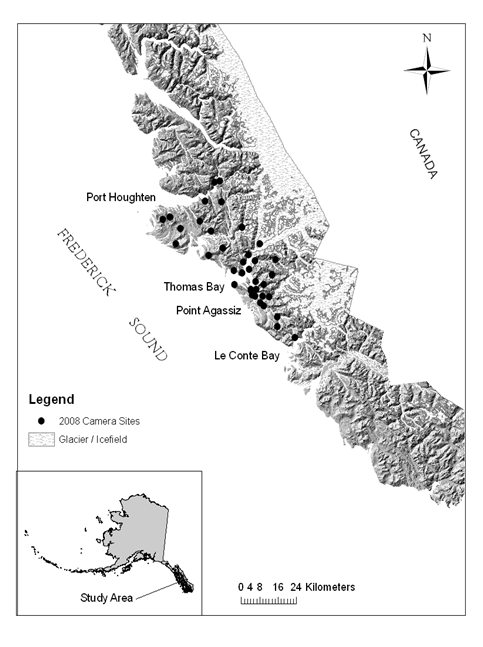
\includegraphics[height=3in]{Ch4/figs/wolverinelocs}
\end{center}
\caption{Wolverine camera trap locations from \citet{magoun_etal:2011}.
XXXXX this figure is way too small. Also, I would take out some of the
legends in the actual figure and put this into the figure legend
(e.g., what the dots mean and the grey area) XXXXXX
}
\label{scr0.fig.wolverinelocs}
\end{figure}

To carry-out an analysis of these data, we require the matrix of trap
coordinates and the encounter history data.  We store data in the
``scr flat format'' (see sec.  \ref{scr0.sec.formats} above), an
efficient file format which is easily manipulated and also used as the
input file format in {\bf SPACECAP} \citep{gopalaswamy_etal:2012} and
in the {\bf R} package \mbox{\tt SCRbayes} \citep{russell_etal:2012}.
To illustrate this format, the wolverine data are available in the
package \mbox{\tt scrbook} by typing:
\begin{verbatim}
data(wolverine)
\end{verbatim}
which contains a list having elements \mbox{\tt wcaps} and
\mbox{\tt wtraps}.
The ``encounter data file''
\mbox{\tt wcaps}  has 3 columns and 115 rows, each representing a
unique encounter event including the trap identity, the individual
identity and the sample occasion index (\mbox{\tt sample}).
The first 10 rows of this matrix are as
follows:
{\small
\begin{verbatim}
> wolverine$wcaps[1:10,]
       trapid individual sample
  [1,]      1          2    127
  [2,]      1          2    128
  [3,]      1          2    129
  [4,]      1         18    130
  [5,]      2          3    106
  [6,]      2         18    104
  [7,]      5          5     73
  [8,]      5          5     89
  [9,]      6         18    117
 [10,]      6         18    118
\end{verbatim}
}
Each row is a unique 
individual/trap encounter, and the 3 variables (columns) are: 
\mbox{\tt trapid} -- an
integer that runs from \mbox{\tt 1:ntraps}, \mbox{\tt individual} runs from
\mbox{\tt 1:nind} and
\mbox{\tt sample} 
runs from \mbox{\tt 1:nperiods}. Often (as the case here) \mbox{\tt
  sample} 
will
correspond to daily sample intervals. The variable \mbox{\tt trapid} will have to
correspond to the row of a matrix containing the trap coordinates - in
this case the file \mbox{\tt wtraps} which we describe further below.

Note that the information provided in this encounter data file
\mbox{\tt wcaps}
does not represent a completely informative summary
of the data. For example, if no individuals were captured in a certain
trap or during a certain period, then this compact data format will
have no record. Thus we will need to know \mbox{\tt ntraps} XXXX? in general, we have multiple definitions of these things and we need to be consistentXXXXXX and \mbox{\tt nperiods} when
reformatting this SCR data format into a 2-d encounter frequency
matrix or 3-d array. In addition, the encounter data file does not
provide information about which periods each trap was operated. This
additional information is also necessary as the trap-specific sample
sizes must be passed to {\bf BUGS} as data. We provide this information in a
2nd data file, along with the trap coordinates, in the 
 ``trap deployment'' file which is described
below.

For our purposes we
need to convert the \mbox{\tt wcaps} file
into the $n \times J$ array of
binomial encounter frequencies, although more general models might
require an encounter-history formulation of the model which requires a
full 3-d array.  To obtain our $n \times J$ encounter frequency
matrix, we do this the hard way by first converting the encounter data
file into a 3-d array and then summarize to trap totals. We have a
handy function \mbox{\tt SCR23darray.fn} which takes the compact
encounter data file with optional arguments  \mbox{\tt ntraps} and \mbox{\tt nperiods}, and
converts it to a 3-d array, and then we use the {\bf R} function
\mbox{\tt apply} to summarize over the ``sample'' period dimension (by
convention here, this is the 2nd dimension). To apply this to the
wolverine
data in order to compute the 3-d array we do this:
{\small
\begin{verbatim}
y3d <-SCR23darray.fn(wolverine$wcaps,wolverine$wtraps)
y <- apply(y3d,c(1,3),sum)
\end{verbatim}
}
See the help file for more information on \mbox{\tt SCR23darray.fn}.
The 3-d array is necessary to fit certain types
of models (e.g., behavioral response) and this is why we sometimes
will require this maximally informative 3-d data format but, here, we
analyze the summarized data.



The other important information needed to fit SCR models is the
``trap deployment'' file
which provides the additional information
not contained in the encounter data file. The traps file has \mbox{\tt
  nperiods} $+ 3$ columns. The first column is assumed to be a trap identifier,
columns 2 and 3 are the easting and northing coordinates (assumed to
be in a Euclidean coordinate system), and columns 4 to (\mbox{\tt nperiods} + 3)
are binary indicators of whether each trap was operational in each
time period. The first 10 rows (out of 37) and 10 columns (out of 167)
of the trap deployment file for the wolverine data are:
{\small
\begin{verbatim}
> wolverine$wtraps[1:10,1:10]

   Easting Northing 1 2 3 4 5 6 7 8 
1   632538  6316012 0 0 0 0 0 0 0 0
2   634822  6316568 1 1 1 1 1 1 1 1
3   638455  6309781 0 0 0 0 0 0 0 0
4   634649  6320016 0 0 0 0 0 0 0 0
5   637738  6313994 0 0 0 0 0 0 0 0
6   625278  6318386 0 0 0 0 0 0 0 0
7   631690  6325157 0 0 0 0 0 0 0 0
8   632631  6316609 0 0 0 0 0 0 0 0
9   631374  6331273 0 0 0 0 0 0 0 0
10  634068  6328575 0 0 0 0 0 0 0 0
\end{verbatim}
}
This tells us that trap 2 was operated in periods (days) 1-7 but the other
traps were not operational during those periods. It is extremely
important to recognize that each trap was operated for a variable
period of time and thus the binomial "sample size" is different for
each, and this needs to be accounted for in the {\bf BUGS} model specification.
To compute the vector of sample sizes $K$, and extract the trap
locations,  we do this:
\begin{verbatim}
traps<- wolverine$wtraps
traplocs<- traps[,1:2]
K<- apply(traps[,3:ncol(traps)],1,sum)
\end{verbatim}
This results in a matrix \mbox{\tt traplocs} which contains the coordinates of
each trap and a vector $K$ containing the number of days that each trap
was operational. We now have all the information required to fit a
basic SCR model in {\bf BUGS}.

Summarizing these data files for the wolverine study, we see that 21
unique individuals were captured a total of 115 times. Most
individuals were captured 1-6 times, with 4, 1, 4, 3, 1, and 2
individuals captured 1-6 times, respectively.  In addition, 1
individual was captured each 8 and 14 times and 2 individuals each
were captured 10 and 13 times.  The number of unique traps that
captured a particular individual ranged from 1-6, with 5, 10, 3, 1, 1,
and 1 individual captured in each of 1-6 traps, respectively, for a
total of 50 unique wolverine-trap encounters.  These numbers might be
hard to get your mind around whereas some tabular summary is often
more convenient. For that it seems natural to tabulate individuals by
trap and total encounter frequencies. The spatial information in SCR
data is based on multi-trap captures\footnote{I will add more 
context here on revision about spatial recaptures, lost recaptures,
ordinary recaptures. Function \mbox{\tt SCRsmy} in \mbox{\tt
  scrbook}}, 
and so, it is informative to
understand how many unique traps each individual is captured in. At
the same time, it is useful to understand how many total captures we have
of each individual because this is, in an intuitive sense, the
effective sample size.  So, we reproduce Table 1 from
\citet{royle_etal:2011jwm} which shows the trap and total encounter
frequencies:

\begin{table} [htp]
  \caption{Individual frequencies of capture for wolverines captured
    in camera traps in Southeast Alaska in 2008. Rows index unique
    trap frequenciesxxxxx $traps or trap frequencies ???$ xxxxxand columns represent total number of captures
    (e.g., we captured 4 individuals 1 time, necessarily in only 1
    trap; we captured 3 individuals 3 times but in 2 different traps).
%% This differs by 1 from Royle et al. 2011 table.
}
\centering
\begin{tabular}{c c c c c c c c c c c}
\hline
 & & & & & & & &  No.&of&captures \\
\hline
No. of traps & 1 & 2 & 3 & 4 & 5 & 6 & 8 & 10 &13 &14 \\
\hline
1 & 4 & 1 & 0 & 0 & 0 & 0 & 0 & 0 & 0 & 0 \\
2 & 0 & 0 & 3 & 2 & 0 & 2 & 1 & 2 & 0 & 0 \\
3 & 0 & 0 & 1 & 1 & 0 & 0 & 0 & 0 & 0 & 1 \\
4 & 0 & 0 & 0 & 0 & 0 & 0 & 0 & 0 & 1 & 0 \\
5 & 0 & 0 & 0 & 0 & 1 & 0 & 0 & 0 & 0 & 0 \\
6 & 0 & 0 & 0 & 0 & 0 & 0 & 0 & 0 & 1 & 0 \\
\hline
\end{tabular}
\end{table}


\subsection{Fitting the model in WinBUGS}

For illustrative purposes here we fit the simplest SCR model with the
half-normal distance function although we revisit these data with more
complex models in later chapters. The model is summarized by the
following 3 components:
\begin{itemize}
\item[(1)] $y_{ij}|{\bf s}_{i} \sim \mbox{Bin}(K, z_{i}\; p_{ij})$
\item[(2)] $p_{ij} = p_{0} \exp(-\alpha1 \; ||{\bf s}_{i}-x_{j}||^2)$
\item[(3)] $ {\bf s}_{i} \sim \mbox{Unif}({\cal S})$
\item[(4)] $ z_{i} \sim \mbox{Bern}(\psi)$
\end{itemize}
We assume customary flat priors on the structural (hyper-) parameters
of the model, $\alpha_{0} = \mbox{logit}(p_{0})$, $\alpha1$ and $\psi$.  It remains to define the
state-space ${\cal S}$. For this, we nested the trap array (Fig.
\ref{scr0.fig.wolverinelocs}) in a
 rectangular state-space extending $20$ km beyond the traps in each cardinal
direction.  We also considered larger state-spaces up to 50 km to
evaluate that choice.  The buffer of the state space should be large
enough so that individuals beyond the state-space boundary are not
likely to be encountered. Thus some knowledge of typical space usage
patterns of the species is useful.  For the analysis, 
we scaled the coordinate system 
so that a unit distance was equal to $10$ km, producing a rectangular
state-space of dimension $9.88 \times 10.5$ units ($area = 10374$ km$^2$)
within which the trap array was nested. As a general rule, we
recommend scaling the state-space so that it is defined near the
origin $(x,y)=(0,0)$. While the scaling of the coordinate system is
theoretically irrelevant, a poorly scaled coordinate system can
produce Markov chains that mix poorly.  For the scaled coordinate
system we fit models for various choices of a rectangular state-space
based on 
buffers from 1.0 to 5.0 units on the scaled coordinate system (10 km to
50 km). In the {\bf R} package \mbox{\tt scrbook} we provide a
function
\mbox{\tt wolvSCR0.fn} which will fit the basic SCR model. For
example, to fit the model in 
{\bf WinBUGS} using data augmentation with $M=300$ potential individuals,
using 3 Markov chains each of 12000 total iterations, discarding the
first 2000 as burn-in, we execute the following {\bf R} commands:
{\small
\begin{verbatim}
library("scrbook")
data(wolverine)
traps<-wolverine$wtraps
y3d <-SCR23darray.fn(wolverine$wcaps,wolverine$wtraps)
toad<-wolvSCR0.fn(y3d,traps,nb=12000,ni=2000,delta=1,M=300)
\end{verbatim}
}
The argument \mbox{\tt delta} determines the buffer size of the state-space.
Note that this analysis takes 
between 1-2 hours on many machines so we recommend trying it out with
lower values of $M$ and fewer iterations.
The output
follows (note, we have a parameter ``sigma'' which we discuss
shortly)\footnote{Final as of 1/11/2012. 
output saved in \mbox{\tt wolv-buffer-study.txt}}:

{\small
\begin{verbatim}
All based on 3 chains, 12k iters, 2k burn, 30k total
Buffer = 10 km
           mean    sd   2.5%    25%    50%    75%  97.5% Rhat n.eff
psi        0.13  0.03   0.08   0.11   0.13   0.15   0.20    1 10000
sigma      0.65  0.06   0.55   0.61   0.64   0.68   0.76    1  1800
p0         0.06  0.01   0.04   0.05   0.06   0.06   0.08    1 20000
N         39.63  6.70  29.00  35.00  39.00  44.00  54.00    1  7100
D          5.92  1.00   4.33   5.22   5.82   6.57   8.06    1  7100
beta       1.23  0.21   0.85   1.08   1.22   1.36   1.66    1  1800
deviance 410.05 12.06 388.70 401.50 409.20 417.80 435.60    1 22000

Buffer = 15 km
 n.sims = 30000 iterations saved
           mean    sd   2.5%    25%    50%    75%  97.5% Rhat n.eff
psi        0.16  0.04   0.10   0.14   0.16   0.19   0.25    1  3800
sigma      0.64  0.06   0.54   0.60   0.64   0.67   0.76    1   510
p0         0.06  0.01   0.04   0.05   0.06   0.06   0.08    1 17000
N         48.77  9.19  34.00  42.00  48.00  54.00  69.00    1  3300
D          5.78  1.09   4.03   4.98   5.69   6.40   8.18    1  3300
beta       1.25  0.21   0.86   1.10   1.24   1.39   1.70    1   510
deviance 411.00 12.16 389.50 402.40 410.30 418.70 437.00    1  5400

Buffer = 20 km
           mean    sd   2.5%    25%    50%    75%  97.5% Rhat n.eff
psi        0.20  0.05   0.12   0.17   0.20   0.23   0.30    1 16000
sigma      0.64  0.06   0.54   0.60   0.63   0.67   0.76    1  1200
p0         0.06  0.01   0.04   0.05   0.06   0.06   0.08    1  1900
N         59.84 11.89  40.00  51.00  59.00  67.00  86.00    1 20000
D          5.77  1.15   3.86   4.92   5.69   6.46   8.29    1 20000
beta       1.26  0.21   0.87   1.11   1.25   1.40   1.71    1  1200
deviance 411.01 12.36 389.10 402.30 410.20 418.80 437.50    1  1500

Buffer = 25 km
           mean    sd   2.5%    25%    50%    75%  97.5% Rhat n.eff
psi        0.24  0.05   0.15   0.20   0.24   0.28   0.36    1  3400
sigma      0.64  0.05   0.54   0.60   0.63   0.67   0.75    1  3600
p0         0.06  0.01   0.04   0.05   0.06   0.06   0.08    1  5000
N         72.40 14.72  47.00  62.00  71.00  81.00 105.00    1  2700
D          5.79  1.18   3.76   4.96   5.67   6.47   8.39    1  2700
beta       1.26  0.21   0.88   1.12   1.25   1.40   1.71    1  3600
deviance 411.35 12.23 389.70 402.70 410.55 419.20 437.20    1 30000

Buffer = 30 km
           mean    sd   2.5%    25%    50%    75%  97.5% Rhat n.eff
psi        0.29  0.06   0.18   0.24   0.28   0.33   0.43    1  3100
sigma      0.63  0.05   0.54   0.60   0.63   0.67   0.75    1  5600
p0         0.06  0.01   0.04   0.05   0.06   0.06   0.08    1 11000
N         86.42 17.98  56.00  74.00  85.00  97.00 126.02    1  3900
D          5.82  1.21   3.77   4.98   5.72   6.53   8.49    1  3900
beta       1.27  0.21   0.88   1.12   1.26   1.41   1.71    1  5600
deviance 411.06 12.37 389.20 402.50 410.20 418.90 437.60    1 10000

Buffer = 35 km
           mean    sd   2.5%    25%    50%    75%  97.5% Rhat n.eff
psi        0.34  0.08   0.21   0.29   0.34   0.39   0.50    1 30000
sigma      0.63  0.05   0.54   0.60   0.63   0.67   0.75    1  4500
p0         0.06  0.01   0.04   0.05   0.06   0.06   0.08    1 24000
N        101.79 21.54  65.00  87.00 100.00 115.00 148.00    1 30000
D          5.85  1.24   3.74   5.00   5.75   6.61   8.51    1 30000
beta       1.27  0.21   0.89   1.12   1.25   1.40   1.70    1  4500
deviance 411.10 12.20 389.50 402.40 410.30 418.90 437.20    1 22000

Buffer = 40 km
           mean    sd   2.5%    25%    50%    75%  97.5% Rhat n.eff
psi        0.39  0.09   0.24   0.33   0.39   0.45   0.60 1.01   480
sigma      0.64  0.05   0.54   0.60   0.63   0.67   0.75 1.01   410
p0         0.06  0.01   0.04   0.05   0.06   0.06   0.08 1.00 21000
N        118.05 26.14  75.00 100.00 116.00 133.00 178.00 1.01   450
D          5.87  1.30   3.73   4.97   5.76   6.61   8.84 1.01   450
beta       1.27  0.21   0.89   1.12   1.25   1.40   1.72 1.01   410
deviance 411.37 12.35 389.30 402.60 410.60 419.30 437.50 1.00  9700

Buffer = 45 km
           mean    sd   2.5%    25%    50%    75%  97.5% Rhat n.eff
psi        0.45  0.10   0.28   0.38   0.44   0.51   0.66    1  3600
sigma      0.64  0.05   0.54   0.60   0.63   0.67   0.75    1 10000
p0         0.06  0.01   0.04   0.05   0.06   0.06   0.08    1  8100
N        134.43 28.68  85.00 114.00 132.00 153.00 196.00    1  3300
D          5.83  1.24   3.68   4.94   5.72   6.63   8.50    1  3300
beta       1.26  0.21   0.88   1.11   1.24   1.39   1.69    1 10000
deviance 411.36 12.19 389.60 402.70 410.60 419.10 437.30    1  9400

Buffer = 50 km
           mean    sd   2.5%    25%    50%    75%  97.5% Rhat n.eff
psi        0.51  0.11   0.31   0.43   0.50   0.57   0.74    1  3200
sigma      0.63  0.05   0.54   0.60   0.63   0.67   0.75    1  4700
p0         0.06  0.01   0.04   0.05   0.06   0.06   0.08    1  3300
N        151.61 31.65  96.00 129.00 149.00 172.00 221.00    1  3400
D          5.79  1.21   3.66   4.92   5.69   6.56   8.43    1  3400
beta       1.27  0.21   0.89   1.12   1.25   1.40   1.70    1  4700
deviance 410.81 12.18 389.20 402.30 410.10 418.50 436.70    1 30000

Buffer = 55 km 
           mean    sd   2.5%    25%    50%    75%  97.5% Rhat n.eff
psi        0.56  0.12   0.35   0.48   0.55   0.64   0.82 1.01   260
sigma      0.64  0.05   0.54   0.60   0.63   0.67   0.76 1.00  1600
p0         0.06  0.01   0.04   0.05   0.06   0.06   0.08 1.00 30000
N        169.28 35.81 108.00 143.00 166.00 192.00 247.00 1.01   260
D          5.73  1.21   3.66   4.84   5.62   6.50   8.36 1.01   260
beta       1.25  0.21   0.88   1.11   1.24   1.39   1.69 1.00  1600
deviance 411.28 12.38 389.40 402.60 410.50 419.10 437.50 1.00 26000
\end{verbatim}
}

We see that the estimated density is roughly consistent as we increase
the state-space buffer from $15$ to $50$ $km$. We do note that the data
augmentation parameter $\psi$ (and, correspondingly, $N$) increase with
the size of the state space in accordance with the deterministic
relationship $N= D*A$. However, density is more or less constant as we
increase the size of the state-space beyond a certain point.  For the
10 $km$ state-space buffer, we see a slight effect on the posterior
distribution of $D$. This is not a bug but rather a feature. As we noted
above, the state-space is part of the model.


\subsection{Thoughts on the Wolverine Analysis}

Our point estimate of wolverine density from this study, using the
posterior mean from the state-space based on the 20
$km$ buffer, is 
approximately $5.77$ individuals/1000 $km^2$ with  a 95\% posterior
interval of $[3.86, 8.29]$. Density is estimated imprecisely
which might not be surprising given the low sample size ($n=21$
individuals!). This seems to be a basic feature of carnivore studies
although it should not (in our view) preclude the study of their
populations nor attempts to estimate density or vital rates.

One thing we haven't talked about yet is that we can calibrate the
desired size of the state-space by looking at the estimated home range
radius of the species. For some models it is possible to convert the
parameter $\alpha1$ directly into the home range radius (sec. 
XXX MISSING XYZ). For the half-normal model we interpret the half-normal scale
parameter $\sigma$, which is related to $\alpha1$ by $\alpha1 =
1/(2\sigma^2)$, as the radius of a bivariate normal movement model. 
In this case $\sigma = 1.82$ standardized units, which corresponds to 18.2 $km$ and translates into a home range area of XXXX MISSING XXXXX. 

It is worth thinking about this model, and these estimates, computed
under a rectangular state space roughly centered over the trapping
array (Fig. \ref{scr0.fig.wolverinelocs}).
Does it make sense to define the state-space to
include, for example, ocean? What are the possible consequences of
this? What can we do about it?  There's no reason at all that the
state space has to be a regular polygon -- we defined it as such here
strictly for convenience and for ease of implementation in {\bf WinBUGS}
where it enables us to specify the prior for the activity centers as
uniform priors for each coordinate.  While it would be possible to
define a more realistic state-space using some general polygon GIS coverage, it
might take some effort to implement that in the {\bf BUGS} language
but it is not difficult to devise custom MCMC algorithms to do that
(see Chapt. \ref{chapt.mcmc}).
Alternatively, we recommend
using a discrete representation of the state-space -- i.e., approximate
${\cal S}$ by a grid of $G$ points. We discuss this in sec. 
\ref{scr0.sec.discrete}.

\section{The Implied Model of Space Usage:
Implied resource selection model? 
Implied home range model?
}
\label{sec.scr0.implied}

We have implied a few times that the model for detection probability
is somehow related to animal ``home range'' somehow. Here 
we explore the nature of that relationship.  While we have used the
term ``home range'' and other jargon (territory, activity center,
etc..) almost interchangeably, what we really mean to imply is
something that would be more more clearly identified as ``space
usage'' which we view in a manner equivalent to what is normally
called resource selection. If the resource is only space, i.e., with
no explicit covariates, then space usage is a more descriptive term
but, otherwise (Chapt. XXXX) we take the term as being analogous to
 ``resource selection''.

We believe that thinking about detection models as models of
space usage of animals is more sensible and interpretable in the manner
that we describe here.  A given detection model will imply a a model
of space usage -- amount and extent of area used some prescribed
percentage of the time -- i.e., 95\% of animal movements are within
some distance from an individual's activity center. 
In that sense, i.e., if we equate that area to ``home
range'', then the detection model implies a model of home range. In
other words, there is an implicit home range model underlying a given
detection probability model. 

i.e., ``how much space encompases 95\% of the movement outcomes of an
individual -- or the space used.''

Intuitively, the detection function of SCR models is related to home
range area or space usage of individuals.  This is because we
interpret the detection model as the composite of two processes -
movement about the home range i.e., space usage, and detection {\it conditional on use} (see
chapter 1.XYZ). Formally we decompose encounter probability according
to (all things conditional on ${\bf s}$ here):
\[
 \Pr(encounter at x|s) = \Pr(encounter | usage of x, s) \Pr(usage of x|s).
\]


How do we chararacterize $Pr(usage)$?  First of all we note that it is
not a proability distribution on $x$ like a classical RSF. Instead,
think of an animal using space for some period of time and accuulating
a history of space usage (being a bunch of values of $x$) and we
random sample a single value. Define $\pi(x|s)$ to be a probability
distribution of that value, i.e., $\pi(x|s)$ {\it is} a probability
distribution of $x$. following standard notions of this stuff we
use this function here:
\[
\pi(x|s) =  \frac{ exp(  -d(s,x)^{2}/(2\sigma^{2})) }
{ \sum_{x} exp(  -d(s,x)^{2}/(2\sigma^{2})) }
\]
therefore clearly the space used by an individual will be proportional
to whatever kernel we stick in for the numerator. The customary
choice, in RSF literature, is to use the negative exponential function
but here we have the Gaussian kernel because we like that.

This is a pdf of $x$ and in sampling a populationi of individuals
using traps or other devices we set them out and they accumulate
potential detections over a period of time. Thus whether or not a
point $x$ is {\it used} (at all) depends on some unknown rate of use
by the individual over whatever period of time the devices are
active. This is something we can't hope to estimate or model in most
cases but we imagine that over a period of time usage is characterized
by a rate of usage $\lambda_{0}$ so that amount of usage of $x$ is
\[
m(x,s) = Poisson(\lambda_{0} \pi(x|s) ) 
\]
which isn't really an important assumption because note that by
conditioning on the total again it retains the (natural) multionomial
distribution. So we ask ``if a guy uses space 100 times, where is that
space being used?'' and the histogram of usage is proportional to
$\pi(x|s)$. But over time timee intrval we expect this amount to be
random and then whether we detect a guy or not at $x$ occurs if
$m(x|s)>0$. That is
\[
Pr(y=1) = 1-exp(-\lambda_{0} \pi(x|s))
\]
Some call this a ``hazard model.''  This is why we like the cloglog
link function in XXXXX (royle et al. 2009ecol).
So this all comes about by introducing a latent process of ``usage''
accumulating over time.    
We could just as well say $Pr(y=1) \propto \pi(x|s)$ which is the
half-normal model. 


Ok back to this thing: 
\[
 \Pr(encounter at x|s) = Pr(encounter | usge of x,s) Pr(usage of x|s).
\]
Therefore, if we imagine that encounter probability was perfect,
everywhere, and animals moved around according to some bivariate
distribution $\Pr(movement to x | s) = g(x,s)$ then a sensible summary
of home range (or space usage) is the area that contains 95\% of the
mass of $g(x,s)$. i.e., 95\% of all animal locations.  In SCR models it
is not always so clear how to compute this because (1) most detection
functions do not correspond to a specific bivariate movement
distribution g(x,s) and (2) we only get to observe ``movement outcomes''
where we happen to have traps, and even then we don't observe those
perfectly (just when the movement outcome is near a trap).


\subsection{Bivariate normal case}  

There is (at least) one detection model that allows a direct
conversion to a home range model based on space usage. This is the
model that arises under a bivariate normal movement model.  In fact there are two representations for this detection model. The obvious one is:
\[
p(x,s) = \lambda_{0} \exp(-\theta*||{\bf x}-{\bf s}||^2)         
\]
Thinking about this under our decomposition mentioned above, i.e., 
\[
Pr(detection at x | s) = Pr(detection | x used)Pr(x used | s)
\]
It seems reasonable to imagine that the conditional probability of
detection is constant or at least not dependent on ${\bf s}$ (but it
might depend on ${\bf x}$, the trap location, and that would be ok,
see chapt. XXXXX) and we therefore recognize the 2nd part is the
kernel of a bivariate probability distribution which is an explicit
movement model that is widely used.  For the bivariate normal case
then:
\[
\Pr(detection at x | s) = lam0*const*exp(- (1/(2*sigma*sigma))*dist(x,s)^2)
		            =  p0*exp(- (1/(2*sigma*sigma))*dist(x,s)^2)
\]
Here ``const'' is the part of the bivariate normal density that allows
it to integrate to 1. Therefore the effective local encounter rate is
the product of the conditional probability of detection lam0 and this
normalizing constant.

Under this model we can compute precisely the effectively home range
area. In particular, imagining that movement outcomes are bivariate
normal then $||{\bf x}-{\bf s}||^2$ has a chi-square distribution with
2 d.f. and so we need to find the constant $B(\alpha)$ such that
$\Pr(d\le B(\alpha)) = 1-\alpha$, i.e, the constant $B(\alpha)$ that
encloses 95\% of all realized distances. The constant $B(\alpha) =
\sigma*\sqrt{q(2,\alpha)}$. For $\alpha=.05$, $q(2,\alpha) = 5.99$ so
as an example for $\sigma=1$, $B(\alpha) = 1*\sqrt{5.99} = 2.447$ and
therefore 95\% of the movement outcomes will be within 2.447 units of
the home range center. So the basic idea is that we can estimate
``sigma'' by fitting the detection model above (either form) and
plugging it into this expression for $B(\alpha)$ to obtain the home
range radius that contains 95\% of movement outcomes.

\subsection{Hazard formulation}

An alternative bivariate normal model is based on a bivariate normal hazard rate:
\[
p(x,s) = 1-exp(-lam0*exp(-beta*||x-s||^2))
\]
It is perhaps not immediately clear why or even whether these should
produce the same home range area for a given beta, but it turns out
they do!  Its not obvious to me why, so a little bit of analysis is in
order for sure.

\subsection{Empirical analysis}

For many detection models we can compute the 95\% area empirically
by taking a fine grid of points and 
either simulating movement outcomes with probabilities proportional to
$p(x,s)$ and accumulating area around ${\bf s}$ or else we can do this precisely
by finding the distance $||x-s||$ within which 95\% of all movements are
concentrated. 

Under any detection model, movement outcomes will occur
in proportion to $p(x,s)$ and so we can define probabilities according
to:
\[
 \pi(x|s) =\frac{p(x,s)}{\sum_{x} p(x,s) }
\]
i.e., under the 2-part decomposition noted above, the use 
distribution has to have probabilities $\pi({\bf x}|{\bf s})$. In
other words, $\pi({\bf x}|{\bf s})$ is a discrete representation of
this movement distribution.  Given the probabilities $\pi({\bf
  x},{\bf s})$ for all ${\bf x}$ we can find the value of ${\bf x}_{0}$ such that
$\sum_{{\bf x}_0 s.t. ||x0-s||} \pi({\bf x},{\bf s}) \le 0.95$.
Here is an algorithm for doing that (below). But first we simulate some data.

{\small
\begin{verbatim}
# source SCR utility functions
source("utilities.R")

# individual centered at (3,3) with 10000 "potential trap" locations
s<-c(3,3)
x1<- rep(seq(0,6,,100),100)
x2<- sort(rep(seq(0,6,,100),100))
delta<- min(diff(x1[1:10]))
area<- ( (6+delta/2)^2)/10000

# plot those trap locations
X<-cbind(x1,x2)
plot(X,pch=".")

# compute distances and encounter probabilities under some model
D<-sqrt(  ( s[1]-x1)^2  + (s[2]-x2)^2)
sigma<- .396
lp<-  -2.72 -(1/(2*sigma*sigma))*D*D
p<- 1-exp(-exp(lp))
# 2 alternative link functions
#p<-  exp(lp)
#p<- expit(lp)

# plot this surface
spatial.plot(X,p)

# use these probabilities to simulate movement outcomes
pi.probs <- p/sum(p)
\end{verbatim}
}

Next we find the value of ${\bf x}_0$ such that $\sum_{x<=x0}
\pi({\bf x}|{\bf s}) = 0.95$. We do this by starting at some small
value of ${\bf x}_0$ and then summing the appropriate values of
$\pi$. If the total is $< 0.95$ then we increase ${\bf x}_0$ by a
little bit (1\% below), otherwise if the total area $\ge 0.95$ then we
break out of the loop. Here a crude root-finding algorithm:

\begin{verbatim}
# find area that contains 95% of movements
x0<-.2
repeat{
in.hr<- D<=x0
total<- sum(pi.probs[in.hr])  
cat("Total area: ",total,fill=TRUE)
if(total>=.95) {
print(x0)    # if condition is met, break
break
}
x0<-x0*1.01  # otherwise increase x0
}
\end{verbatim}

If we execute this root-finding code for the simulated data above we
have the following, where the number output is the desired ${\bf x}_0$:
\begin{verbatim}
Total area:  0.9484948
Total area:  0.9500548
[1] 0.973035
\end{verbatim}

What this means is that ${\bf x}_0 = 0.973$ is the radius that
encloses about 95\% of all movements under the model above. Therefore
the area is about $\pi*.973*.973 = 2.97 \approx 3.0$.
You can change the intercept of the model and find that it has no affect. I don't know if that works out across all classes of models or not. Note that the intercept never affects $p$ multiplicatively and so its not obvious (to me) that it shouldn't have an affect (except somewhat intuitively perhaps).

The point of doing this is that we can now apply this process of simulating data to find the 95\% home range area for any detection model with prescribed parameter values.  Similarly, we can also work backwards. That is: For any desired 95\% home range area, we can find the coefficient on distance that produces that home range area (assuming intercept to have no affect). Here is a function for doing that:

First, define an objective function to find the root of. This is a
function of $\sigma$ and also the target home range area (``target'')
which is fixed:
\begin{verbatim}
obj<-function(sigma,target= 3 ){
a<-1/(2*sigma*sigma)
lp<- -2 -a*D*D
p<- 1-exp(-exp(lp))

pi.probs<- p/sum(p)
x0<-.1
repeat{
in.hr<- D<=k
total<- sum(pi.probs[in.hr])  
#cat("Total area: ",total,fill=TRUE)
if(total>=.95) {
print(x0)
break
}
x0<-x0*1.01
}
hr.area<- pi*x0*x0
print(hr.area)
ss<-  (hr.area - target)^2
ss
}
\end{verbatim}


Now we use the {\bf R} function optimize to locate the optimal value
of $\sigma$ - optimal here being the value of $\sigma$  that makes
home range area minus ``target''  equal to 0:
\begin{verbatim}
tmp<-optimize(obj,interval=c(.1,5),target=3)
sigma.best<- tmp$minimum

> sigma.best
[1] 0.3957799
\end{verbatim}

We see this is equal to 0.396 which is the value we simulated data from above - so things seem to be working in an orderly manner. 

\subsection{Why do we care about this stuff?}

One important reason that we need to be able to deduce ``home range
area'' from a detection model is so that we can compare different
models on the same biological footing. 
As we noted somewhere else (XXXX in ch 4) the scale parameter $\sigma$
relateds to 95\% area in a different manner under each detection
function and so we want to be able to convert different models to the
same currency. 


RSF/telemetry data: In chapter XXXX 
we consider the case in which a sample of individuals produces encounter history data suitable for SCR models and, in addition, we have telemetry relocations on a subset of individuals - within the same population or not, it probably doesn't matter.  We assume the telemetry fixes are made sufficiently far apart so that the locations represent independent movement outcomes of individuals within their home range [note: otherwise we need to devise a model for correlated outcomes which is difficult, except in the bivariate normal situation].

Conceptually we regard these two data sets as independent. Let $y[i]$
denote the individual encounter history data for individual i and let
$u[m,t=1,\ldots,T]$ denote the telemetry locations for individual m. If
we have a common model in terms of space usage then we can combine the
two data sources to improve information.  Bivariate normal model is
covered in chapter XXXX but we can also, I think, handle the general
case: Some other detection probability models probably do correspond
to specific bivariate distributions that can be evaluated and
simulated from directly. In general, we can view the telemetry
outcomes u[i,t] as realizations of a point process with intensity
function
\[
\pi(x,s) = p(x,s)/[ \int_{x} p(x,s) ]
\]
Which allows us to analyze models with auxiliary data by MCMC or directly by likelihood.



Modeling space usage. We imagine that each pixel $x$ has a covariate
associated with it and the probability of an individual going there
should be a function of that covariate..... this is different than
Richard's chapter 14 stuff because we are thinking here of modeling
variation {\it within} a home-range. 


\section{Constructing Density Maps}
\label{scr0.sec.mapping}

One of the most useful aspects of SCR models is that they are
parameterized in terms of individual locations - i.e., {\it where}
each individual lives -- and, thus, we can compute many useful or
interesting summaries of the activity centers.  For example, we can
make a spatial density plot by tallying up the number of activity
centers ${\bf s}_{i}$ in pixels  of arbitrary size and then producing a
nice multi-color spatial plot of those which, we find, increases the
acceptance probability of your manuscripts by a substantial amount.
We discussed in Chapt. \ref{chapt.glms} the idea of estimating derived
parameters from MCMC output. In SCR models, there are many derived
parameters that are functions of the latent point locations $({\bf
  s}_{1},\ldots, {\bf s}_{N})$. In the present context, the number of
individuals living in any well-defined polygon is a derived
parameter. Specifically, let $B({\bf x})$ indicate a pixel centered at
${\bf x}$ then
\[
N({\bf x})=\sum_{i} I({\bf s}_{i} \in B({\bf x}))
\]
XXXXXX say that I() is the indicator function XXXX

is the population size of pixel XXX change box to pixel XXXXX $B({\bf x})$, and $D({\bf x}) = N({\bf
  x})/||B({\bf x})||$ is the local density. These are just ``derived
parameters'' (see Chapt.  \ref{chapt.glms}) which are estimated from
MCMC output using the appropriate Monte Carlo average. One thing to be
careful about, in the context of models in which $N$ is unknown, is
that, for each MCMC iteration $m$, we only tabulate those activity
centers which correspond to individuals in the sampled
population, i.e., for which the data augmentation variable $z_{i} =
1$.  In this case, we take all of the output for MCMC iterations
$m=1,2,\ldots,\mbox{\tt niter}$ and compute this summary:
\[
   N({\bf x},m) = \sum_{z_{i,m}=1} I(s_{i,m} \in B({\bf x}))
\]
Thus, $N({\bf x},1),N({\bf x},2),\dots,$ is the Markov chain for
parameter $N({\bf x})$.  In what follows we will provide a set of {\bf
  R} commands for doing this calculation and making a basic image
plot from the MCMC output.

{\flushleft \bf Step 1:} Define the center points of each box, $B({\bf
  x})$, or point at which local density will be estimated:
\begin{verbatim}
xg<-seq(Xl,Xu,,50)
yg<-seq(Yl,Yu,,50)
\end{verbatim}

{\flushleft \bf Step 2:} Extract the MCMC histories for the activity
centers and the data augmentation variables.  Note that these are each
$N \times \mbox{\tt niter}$ matrices:
\begin{verbatim}
Sxout<-out$sims.list$s[,,1]
Syout<-out$sims.list$s[,,2]
z<-out$sims.list$z
\end{verbatim}

{\flushleft \bf Step 3:} We associate each coordinate with the proper
box using the {\bf R} command \mbox{\tt cut()}. Note that we keep only
the activity centers for which $z=1$ (i.e., individuals that belong to
the population of size $N$):
\begin{verbatim}
Sxout<-cut(Sxout[z==1],breaks=xg,include.lowest=TRUE)
Syout<-cut(Syout[z==1],breaks=yg,include.lowest=TRUE)
\end{verbatim}

{\flushleft \bf Step 4:} Use the \mbox{\tt table()} command to tally
up how many activity centers are in each $B(x)$:
\begin{verbatim}

Dn<-table(Sxout,Syout)
\end{verbatim}

{\flushleft \bf Step 5:} Use the \mbox{\tt image()} command to display
the resulting matrix.
\begin{verbatim}
image(xg,yg,Dn/nrow(z),col=terrain.colors(10))
\end{verbatim}
Praise the Lord! This map is somewhat useful or at least it looks
pretty and will facilitate the publication of your papers.

It is worth emphasizing here that density maps will not usually appear
uniform despite that we have assumed that activity centers are
uniformly distributed. This is because the observed encounters of
individuals provide direct information about the location of the
$i=1,2,\ldots,n$ activity centers and thus their ``estimated''
locations will be affected by the observations. In a limiting sense,
were we to sample space intensely enough, every individual would be
captured a number of times and we would have considerable information
about all $N$ point locations. Consequently, the uniform prior would
have almost no influence at all on the estimated density surface in
this limiting situation. Thus, in practice, the influence of the
uniformity assumption decreases as the fraction of the population
encountered increases.

{\bf On the non-intuitiveness of \mbox{\tt image()} } -- the {\bf R}
function \mbox{\tt image()}, invoked for a matrix $M$ by \mbox{\tt image(M)}, might
not be very intuitive to some -- it plots $M[1,1]$ in the lower left
corner. If you want $M[]$ to be plotted ``as
you look at it'' then $M[1,1]$ should be in the upper left corner.  We
have a function \mbox{\tt rot()} which does that. If you do \mbox{\tt image(rot(M))} then it
puts it on the monitor as if it was a map you were looking at.  You
can always specify the $x$ and $y-$ labels explicitly as we did above.

{\bf Spatial dot plots } -- Now here is a cruder version based on the
``spatial dot map'' function \mbox{\tt spatial.plot}, which uses
the function \mbox{\tt image.scale()}.
The \mbox{\tt spatial.plot} function requires arguments of point
locations and the resulting value to be displayed:
\begin{verbatim}
spatial.plot<- function(x,y){
 nc<-as.numeric(cut(y,20))
 plot(x,pch=" ")
 points(x,pch=20,col=topo.colors(20)[nc],cex=2)
 image.scale(y,col=topo.colors(20))
}
# To execute the function do this:
spatial.plot(cbind(xg,yg), Dn/nrow(z))
\end{verbatim}

\subsection{Example: Wolverine density map. }
xxxxx$At places like this, where you revisit an earlier example, I would spend 1-2 sentences to remind the reader of what this is about. E.g., say that this is in SE Alaska in 2007 $xxxxxx
The {\bf R} commands for producing density maps from MCMC output of
spatial capture-recapture models is provided in the {\bf R} function
\mbox{\tt SCRdensity} in the package \mbox{\tt scrbook}. 
We used the posterior output from the wolverine model fitted previously
to compute a relatively coarse version of a density map, using a $10 \times
10$ grid (Fig. \ref{scr0.fig.density10x10}) and using a $30 \times 30$
grid (Fig. \ref{scr0.fig.density20x20}) for a fine-scale map. The {\bf R} commands for
producing such a plot (for short MCMC run) are as follows:
{\small
\begin{verbatim}
library("scrbook")
data(wolverine)
traps<-wolverine$wtraps
y3d <-SCR23darray.fn(wolverine$wcaps,wolverine$wtraps)
# this takes 341 seconds on a standard CPU circa 2011
unix.time(bln<-wolvSCR0.fn(y3d,traps,nb=1000,ni=2000,delta=1,M=100))
Sx<-bln$sims.list$s[,,1]
Sy<-bln$sims.list$s[,,2]
w<- bln$sims.list$w
obj<-list(Sx=Sx,Sy=Sy,w=w)
tmp<-SCRdensity(obj,scalein=100,scaleout=100)
\end{verbatim}
In these figures density is
expressed in units of individuals per $100$ $km^2$, while the area of
the pixels is about 103.7 $km^2$ and 11.5 $km^2$, respectively. That
calculation is based on:
\begin{verbatim}
> total.area<- (Yu-Yl)*(Xu-Xl)*100
> total.area/(10*10)
[1] 103.7427
> total.area/(30*30)
[1] 11.52697
\end{verbatim}

A couple of things are worth noting: First is that as we move away
from ``where the data live'' - away from the trap array - we see that
the density approaches the mean density. This is a property of the
estimator as long as the ``detection function'' decreases sufficiently
rapidly as a function of distance.
Relatedly, it is also a property of statistical smoothers
such as splines, kernel smoothers, and regression smoothers -
predictions tend toward the global mean as the influence of data
diminishes. Another way to think of it is that it is a consequence of
the prior - which imposes uniformity, and as you get far away from the
data, the predictions tend to the prior. xxxxx$is this correct ? I would have thought, they tend to the mean of what the prior AND the data say it should be ?$ xxxxx The other thing to note about
this map is that density is not $0$ over water (although the coastline
is not shown). This might be perplexing
to some who are fairly certain that wolverines do not like
water. However, there is nothing about the model that recognizes water
from non-water and so the model predicts over water {\it as if} it
were habitat similar to that within which the array is nested. But,
all of this is ok as far as estimating density goes and, furthermore,
we can compute valid estimates of $N$ over any well-defined region which
presumably wouldn't include water if we so wished. xxxx$xperhaps might simply say that pixels covered mostly by water could be masked in the plot ?$xxxx

\begin{figure}
\begin{center}
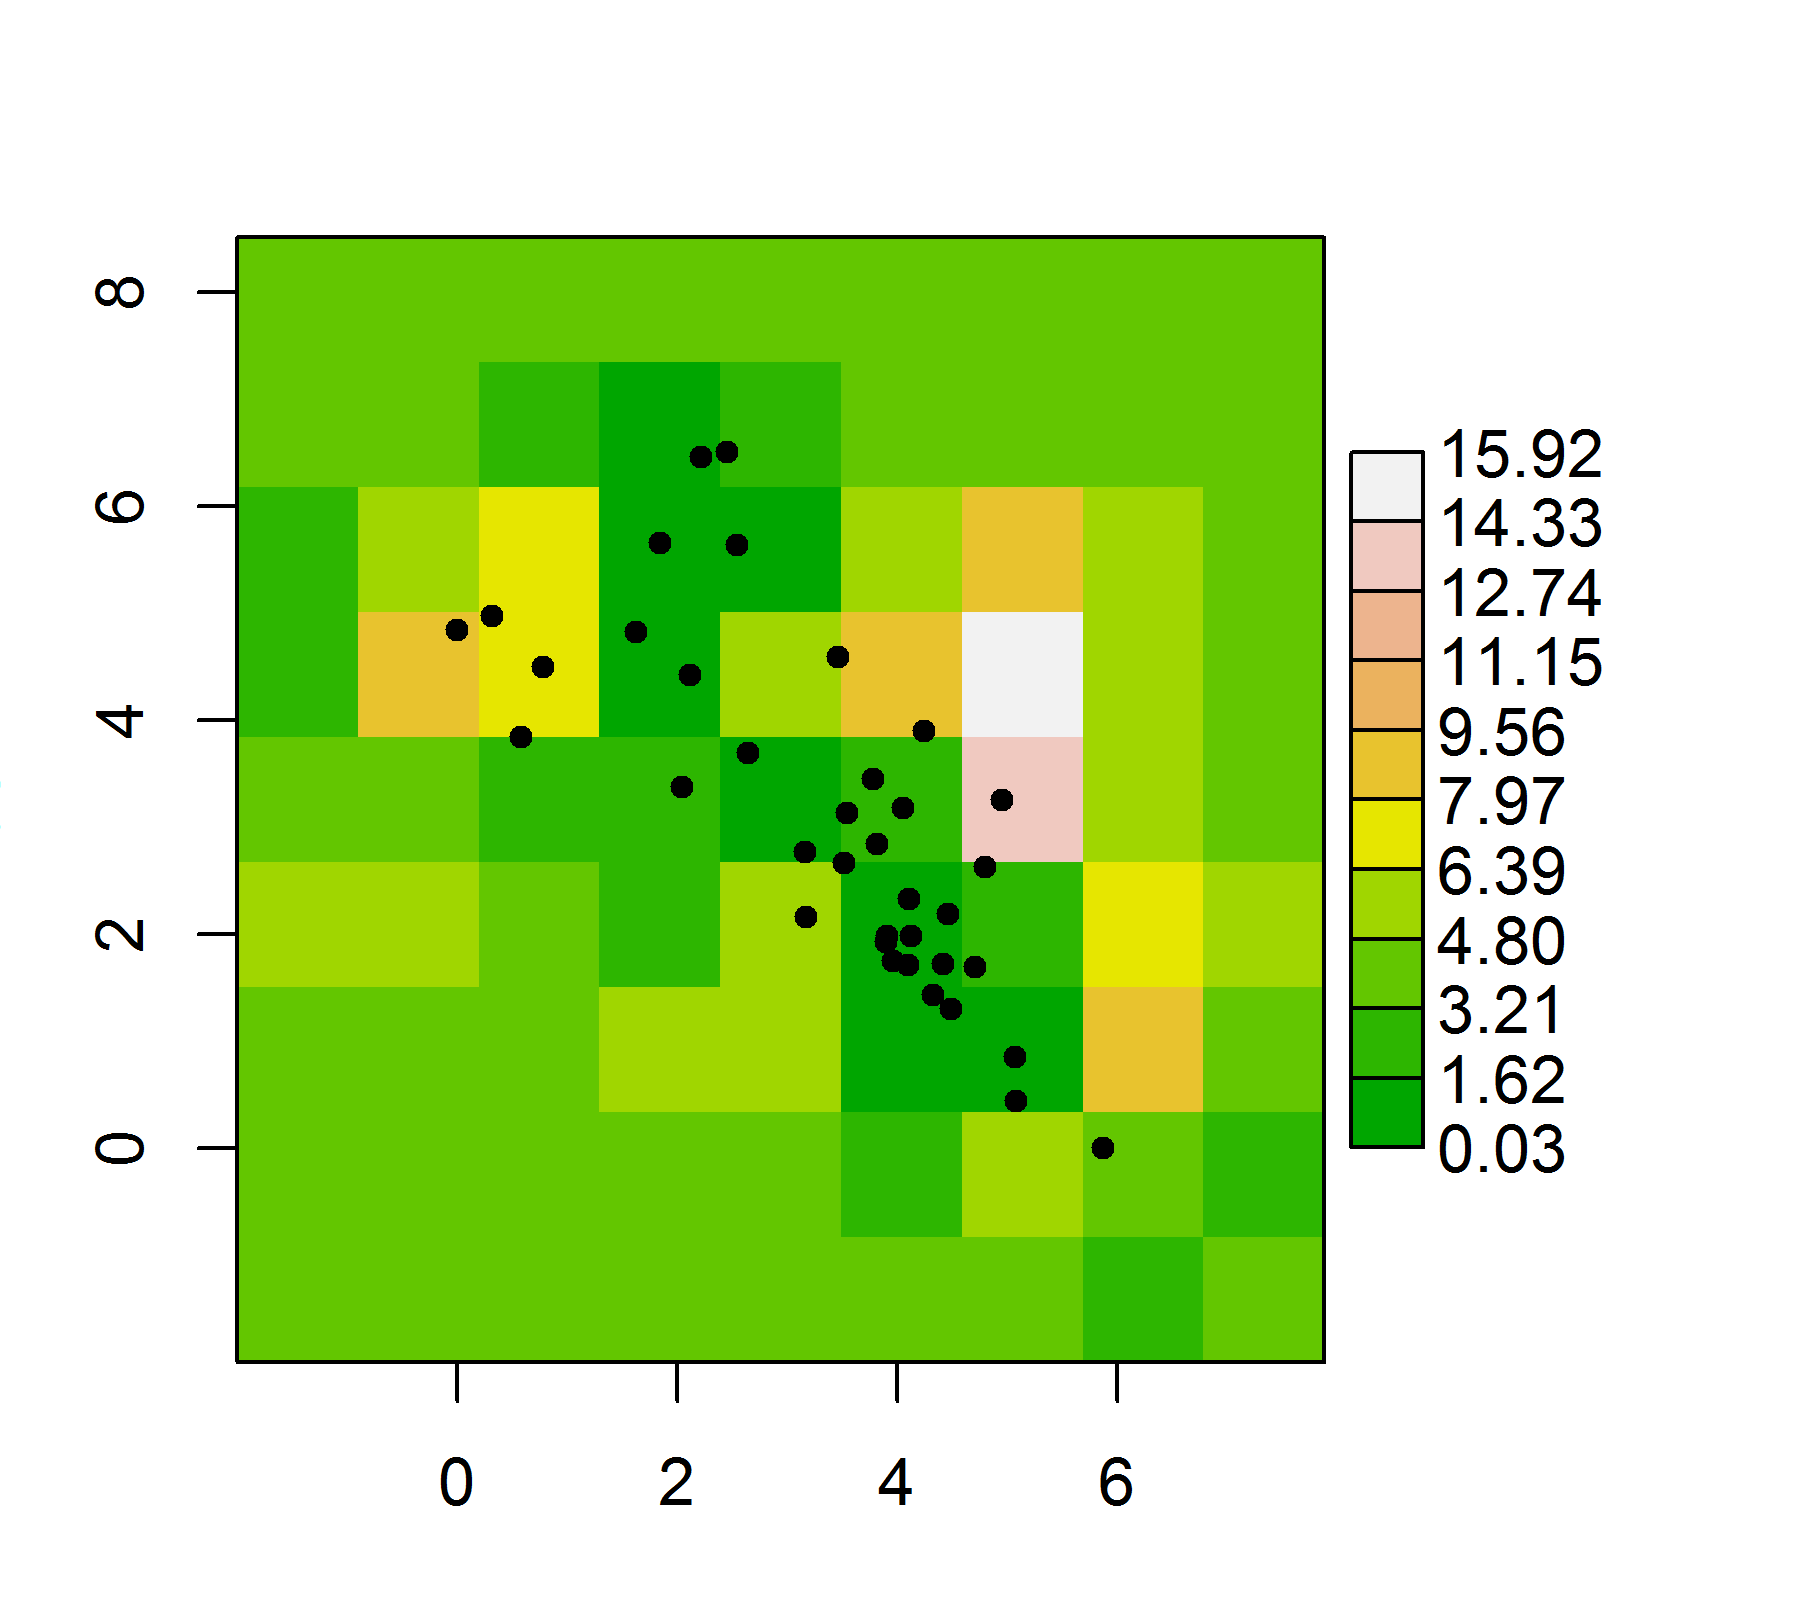
\includegraphics[height=3in,width=3.375in]{Ch4/figs/density10x10}
\end{center}
\caption{Density of wolverines (individuals per 100 $km^2$) in SE Alaska in 2007 based on
  model SCR0. Map grid cells are about 103.7 $km^2$ in area. Dots are the locations of the estimate activity centers of the XXXxxx observed individuals.}
\label{scr0.fig.density10x10}
\end{figure}

\begin{figure}
\begin{center}
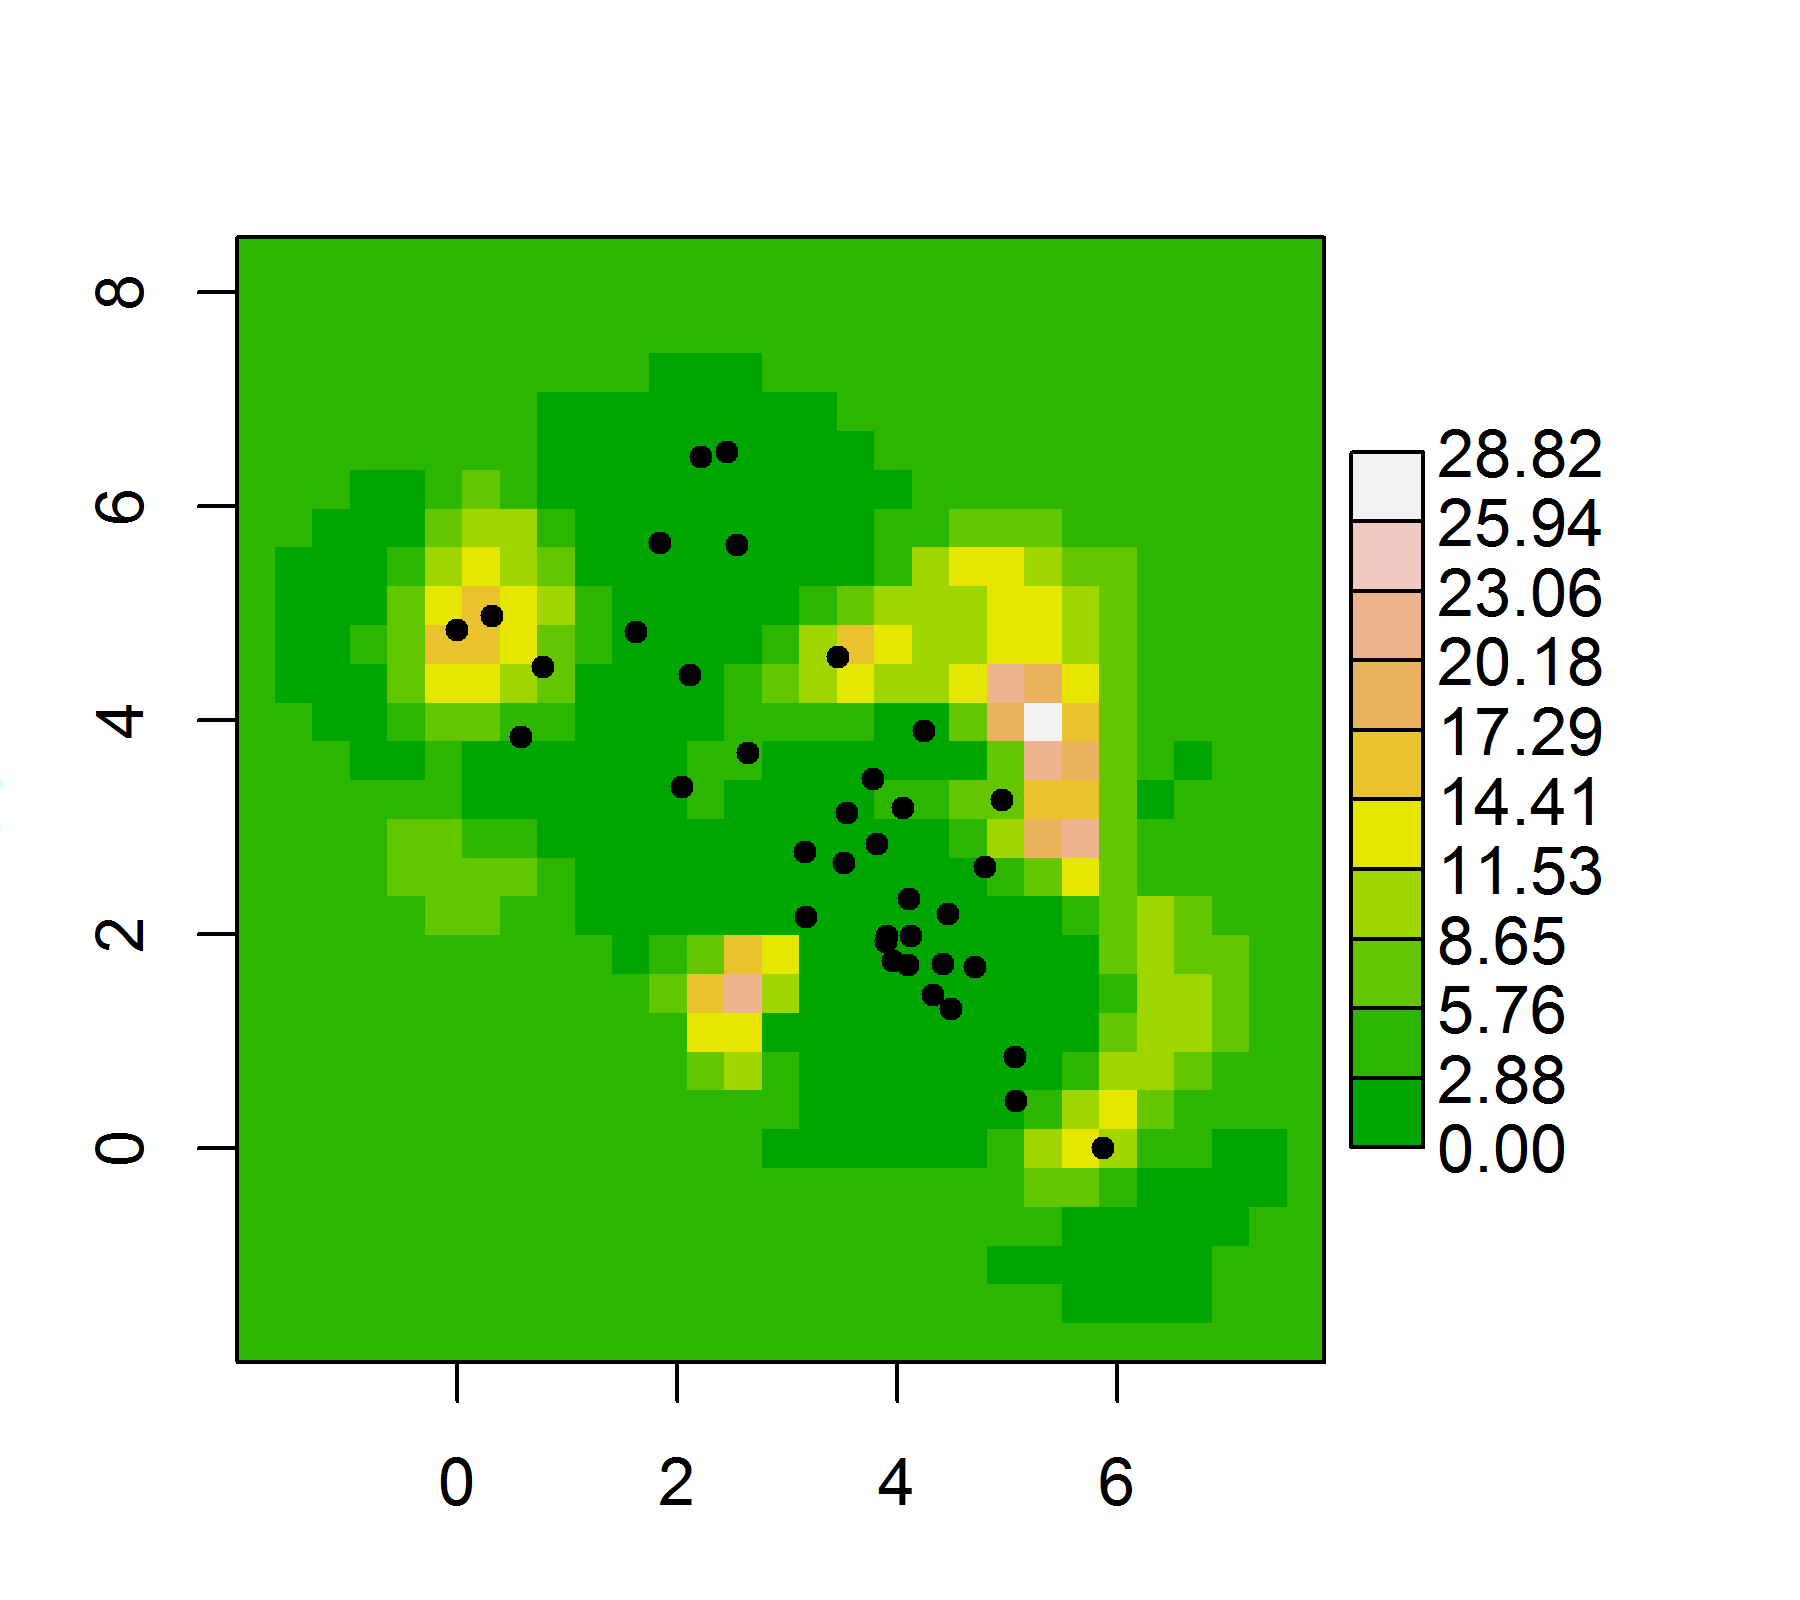
\includegraphics[height=3in,width=3.375in]{Ch4/figs/density30x30}
\end{center}
\caption{Density of wolverines (individuals per 100 $km^2$) based on
  model SCR0. Map grid cells are about 11.5 $km^2$ in area.}
\label{scr0.fig.density20x20}
\end{figure}
xxxxxx
$I would combine Fig. 4.4 and 4.5 in a single two-panel plot and call the plot ?Comparison of the effects of pixel size ...?$
$Then, I would turn color code upside down. I find it more natural to have darker mean a higher value$
$in the scale , one digit is enough$xxxxxxxxxx
xxxxx
$In Fig. 4.5., I find it funny how the estimated high-density areas are mostly away from the HR centers of the observed individuals$xxxxx

\section{Discrete State-Space}
xxxx$more informative title could be ?Allowing for unequal density in discrete state-space?$xxxx
\label{scr0.sec.discrete}

The SCR model developed previously in this chapter assumes that
individual activity centers are distributed uniformly over the
prescribed state-space. Clearly this will not always be a reasonable
assumption. In Chapt. \ref{chapt.state-space} we talk about developing models
that allow explicitly for non-uniformity of the activity centers by
modeling covariate effects on density. A simpler method of affecting
the distribution of activity centers, which we address here, is to
modify the shape and organization of the state-space explicitly. For example, we might
be able to classify the state-space into distinct blocks of habitat
and non-habitat. In that case we can remove the non-habitat from the
state-space and assume uniformity of the activity centers over the
remaining portions judged to be suitable habitat.  There are two ways
to approach this: We can use a regular grid of points to represent the
state-space, i.e., by the set of coordinates ${\bf s}_1, \ldots, {\bf
  s}_{G}$, and assign  equal probabilities to each possible value, or
we can retain the continuous formulation of the state-space but use
basic polygon operations to induce constraints on the state-space. xxxxx$what does this mean ?$xxxxxx We
focus here on the formulation of the basic SCR model in terms of a
discrete state-space but later on (Chapt. \ref{chapt.mcmc} and also
Appendix XYZ) we demonstrate the latter approach based on using
polygon operations to define an irregular state-space.

Use of a discrete state-space can be computationally expensive in {\bf
  WinBUGS}. That said, it isn't too difficult to do the MCMC
calculations in {\bf R} which we discuss briefly in Chapt.
\ref{chapt.mcmc}. The {\bf R} package {\tt SPACECAP}
\citep{gopalaswamy_etal:2011} arose from the {\bf R} implementation of the SCR model  in \citet{royle_etal:2009}.  As we will
see in Chapt. \ref{chapt.mle}, we must prescribe the state-space by a
discrete mesh of points in order to do integrated likelihood and so if
we are using a discrete state-space this can be accommodated directly
in our code for obtaining MLEs.

While clipping out non-habitat seems like a good idea, it?s not obvious
that we accomplish any biologically reasonable objective by doing
so xxxx$why not ?$xxxxx. We might prefer to do it when non-habitat represents a clear-cut
restriction on the state-space such as a reserve boundary or a lake,
ocean or river. But, 
having the capability to do this also causes people to start defining
``habitat'' vs. ``non-habitat'' based on their understanding of the
system whereas it can't be known whether the animal being studied has
the same understanding xxxxxx$I would argue that very often we do have a prett good idea of what is non-habitat$xxxxxx. Moreover, differentiating of the landscape by
habitat or habitat quality probably affects the geometry and
morphology of home ranges much more than the plausible locations of
activity centers. That is, a home range centroid could, in actual
fact, occur in a Walmart parking lot if there is pretty good habitat
around walmart, so there is probably no sense to cut out the Walmart
lot and preclude it as the location for an activity center.  It would
generally be better to include some definition of habitat quality in
the model for the detection probability \citep{royle_etal:2012ecol}
which we address in Chapt. \ref{chapt.ecoldist}.

xxxxxx$This last para doesn?t convince me somehow. I still think that when computing density, you might want to exclude non-habitat. So the guy with its homerange center right on the Walmart parking space should of course count to the estimate of N, but the parking space should be deduced from the state-space. In some way ...$xxxxxx


\subsection{Evaluation of Coarseness of Discrete Approximation}

The coarseness of the state-space should not really have much of an
effect on estimates if the grain is sufficiently fine relative to
typical animal home range sizes.  Why is this?  We have two analogies
that can help us understand this. First is the relationship to model
$M_{h}$.  As noted in sec. \ref{scr0.sec.scrmh} above, we can think
about SCR models as a type of finite mixture
\citep{norris_pollock:1996, pledger:2000} where we are fortunate to be
able to obtain direct information about which group individuals
belong to (group being location of activity center).  In the standard
finite mixture models we typically find that only 1 or a very small
number of groups (e.g., 2 or 3 at the most) can explain really high
levels of heterogeneity and are adequate for most data sets of small
to moderate sample sizes. We therefore expect a similar effect in SCR
models when we discretize the state-space.
We can also
think about discretizing the state-space as being related
to numerical integration where we find (see
Chapt. \ref{chapt.mle}) that we don't need a very fine
grid of support points to evaluate the integral to a reasonable
level of accuracy. We demonstrate this here by reanalyzing simulated
data using a state-space defined by a different numbers of support points.
We provide an {\bf R} script called \mbox{\tt SCR0bayesDss.fn} in the
{\bf R} package \mbox{\tt scrbook}.  We note that for this comparison
we generated the actual activity centers as a continuous random
variable and thus the discrete state-space is, strictly speaking, an
approximation to truth. That said, we regard all state-space
specifications as approximations to truth in the sense that they
represent a component of the SCR model.
Thus the use of any
specific discrete state-space is not intrinsically more ``wrong'' than
any specific continuous representation.

As with our {\bf R} function \mbox{\tt SCR0bayes}, the modification
\mbox{\tt SCR0bayesDss} will use either {\bf WinBUGS} or {\bf
  JAGS}. In addition, it requires a grid resolution argument
(\mbox{\tt ng}) which is the square-root of the number of points in
the state-space grid.
To execute this function we do, for example:
{\small
\begin{verbatim}
library("scrbook")
data<-simSCR0.fn(discard0=TRUE,sd=2013)   # generate data set
out1<-SCR0bayesDss(data,ng=8,M=200,engine="jags",ni=2000,nb=1000) # JAGS
out2<-SCR0bayesDss(data,ng=8,M=200,engine="winbugs",ni=2000,nb=1000) # WinBUGS
\end{verbatim}
}
We fit this model to the same simulated data set for 
$6 \times 6$, $9 \times 9$, $12 \times 12$, $15\times 15$,
$20\times 20$, $25 \times 25$ and $30 \times 30$ state-space grids.
We used 2000 burn, 12000 total iters with 3 chains, yielding a total
of 30000 posterior samples.
For {\bf WinBUGS}, which takes considerably more time (see below),
 we used 3 chains of 5k total with 1k burnin means 12k
total posterior samples.
Summary results for these analyses are shown in
Table XYZ\footnote{To finish later}.

\begin{verbatim}
Table XYZ.Effect of grid coarseness on estimates of N using JAGS and
WinBUGS.

$I would only show results from one engine. COuld simply say in the text that WB was about 5x slower$
JAGS run from rjags
             Mean       SD    NaiveSE  Time-seriesSE  runtime
6    N     109.7717 15.98959 0.0923160    0.377737    1239
9    N     114.4621 16.72025 0.0965344    0.468659    1267
12   N     115.4309 17.12403 0.098866     0.464830    1576
15   N     114.7699 17.0242  0.0982894    0.425238    1638
20   N     116.0370 17.10686 0.0987665    0.486867    1647
25   N     116.3228 16.98323 0.0980527    0.465527    1661
30   N     116.4252 17.4078  0.100504     0.533735    1806
WinBUGS run from R2WinBUGS
             Mean       SD    NaiveSE  Time-seriesSE  runtime
6    N     111.6699 16.61414 0.1516657   0.682008     2274
9    N     114.2294 17.99109 0.1642355   0.833291     4300
12   N     115.9806 17.3843  0.1586964   0.762756     7100
15   N     115.379  17.93721 0.1637436   0.832483    13010

Note: WinBUGS based on fewer samples too!
\end{verbatim}

The results in terms of the posterior summaries are, as we
expect, very similar using {\bf WinBUGS}. However, it was interesting
to note that {\bf WinBUGS} runtime is much worse (note the number of
iterations is lower for {\bf WinBUGS} yet the runtime is much longer)
and, furthermore, it seems to scale with the size of the
discrete state-space grid. While that was expected, it was unexpected
that the runtime of {\bf JAGS} would seem relatively consistent
as we increase the grid size.
We suspect that {\bf WinBUGS} is evaluating the full-conditional for
each activity center at all $G$ possible values whereas it may be that
{\bf JAGS} is evaluating the full-conditional only at a subset of
values or perhaps using previous calculations more effectively.

While this might suggest that one should always use {\bf JAGS} for
this analysis, we found in our analysis of the wolverine (next
section) that {\bf JAGS} could be extremely sensitive to starting
values, producing MCMC algorithms that sometimes simply did not work.

\subsection{Analysis of the wolverine camera trapping data}


We reanalyzed the wolverine data using discrete state-space grids with
points spaced by 2, 4 and 8 km (see in
Fig. \ref{scr0.fig.wolvgrids}). These were constructed from a 40 km
buffered state-space, and deleting the points over water
\citep[see][]{royle_etal:2011jwm}.  Our interest in doing this was to
evaluate the relative influence of grid resolution on estimated
density because the coarser grids will be more efficient from a
computational stand-point and so we would prefer to use them, but
only if there is no strong influence on estimated density.
The density estimates are only slightly different (xxxxsay in which wayxxxxx)is a bit different depending on the grid size. Also the
effectiveness of the MCMC algorithms is pretty remarkably
different. The 2km grid took 6 days to run!

\begin{figure}
\begin{center}
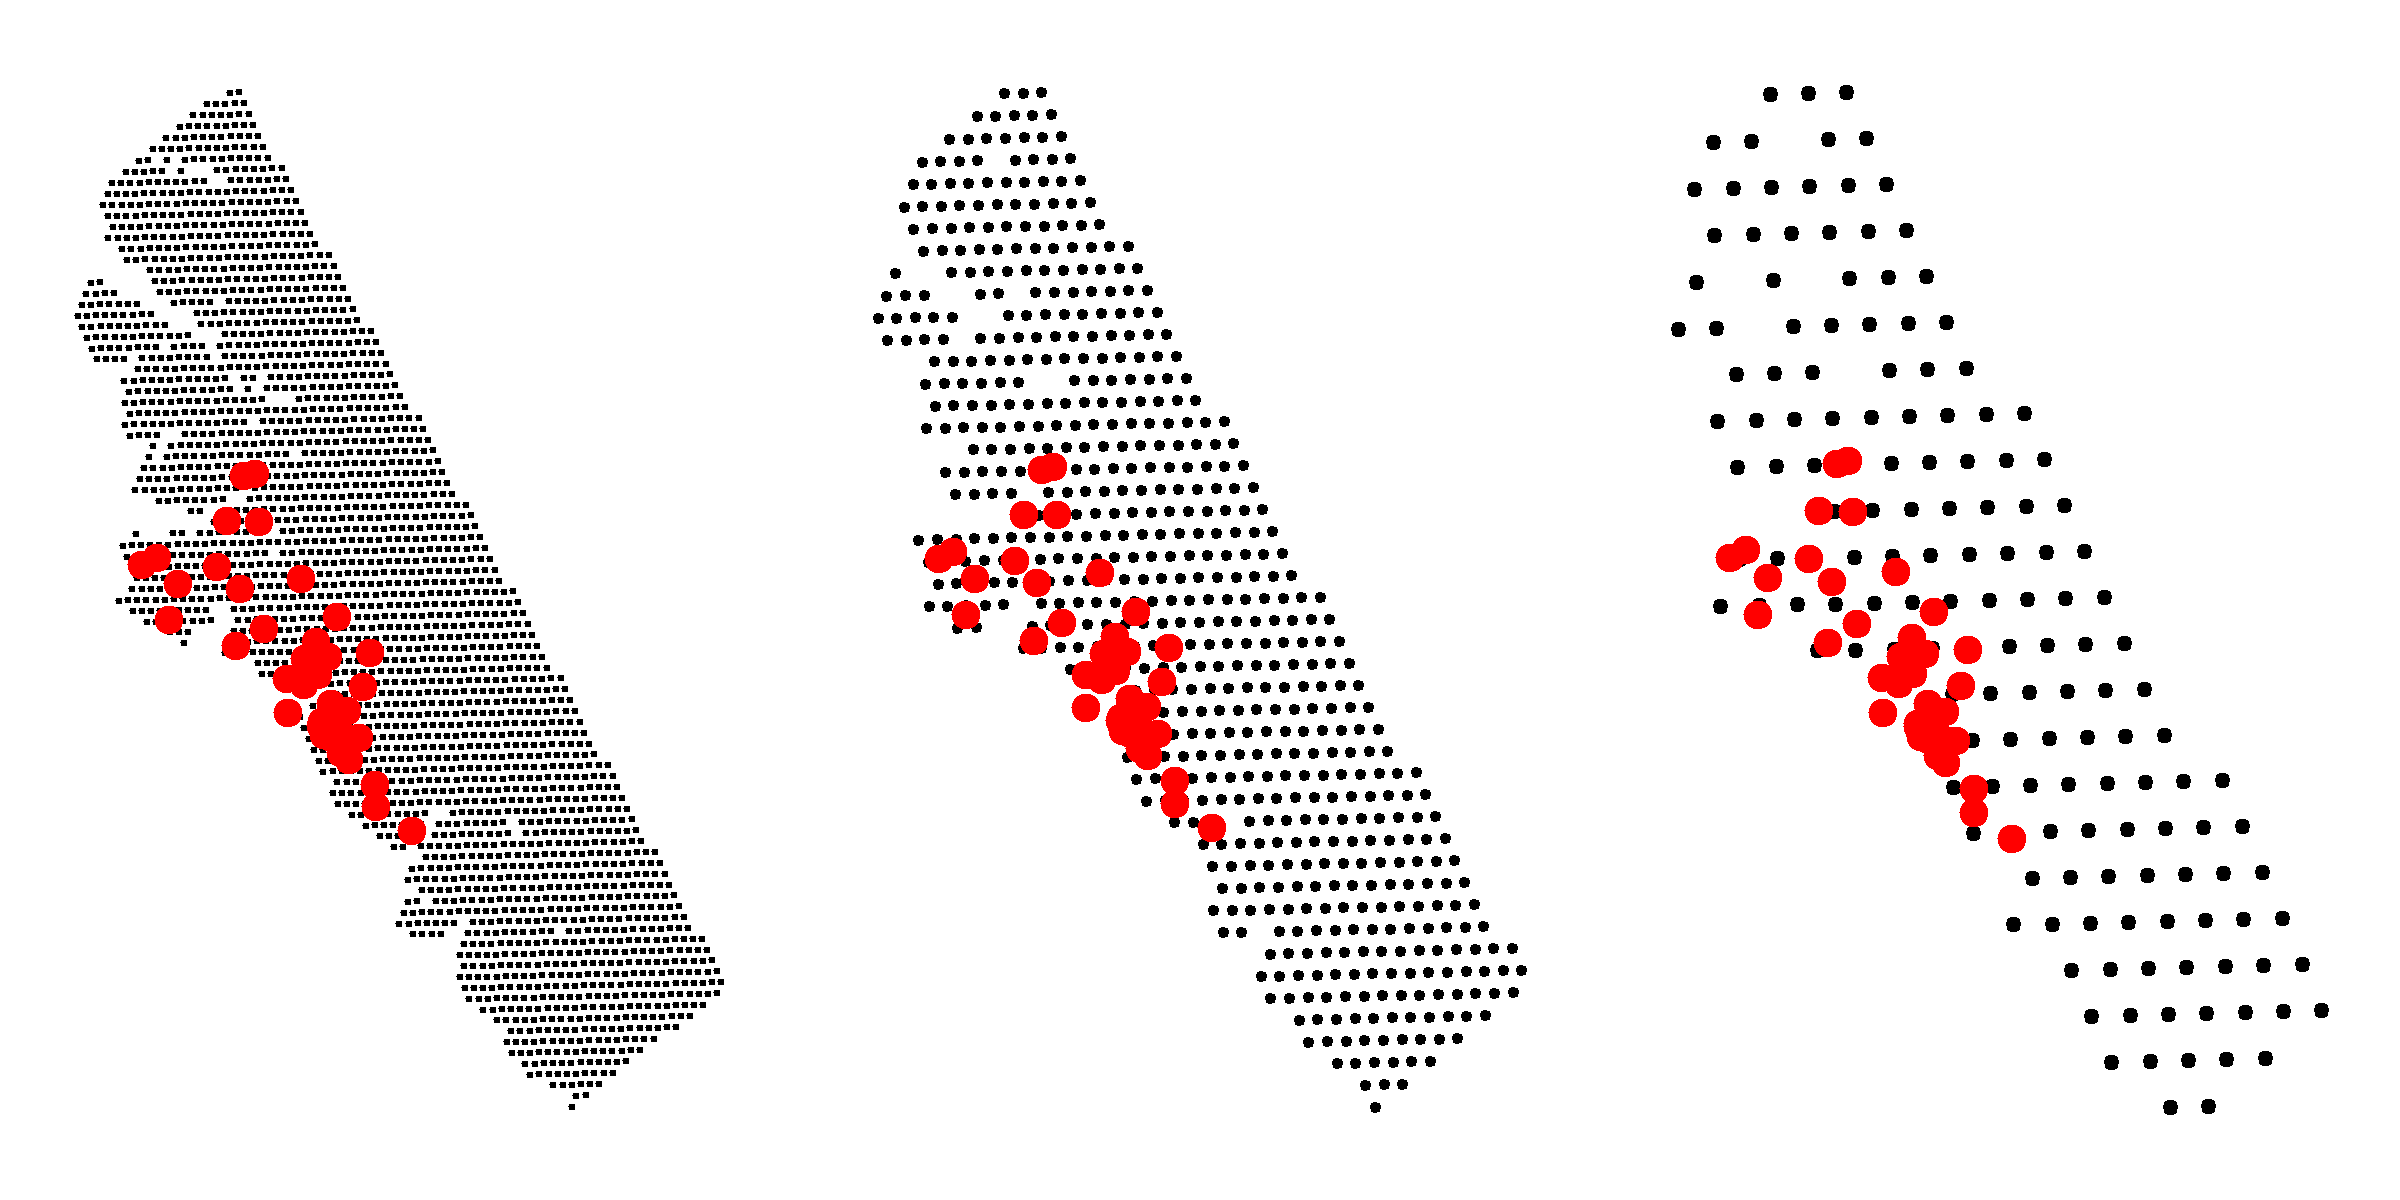
\includegraphics[height=2.5in,width=5in]{Ch4/figs/wolvgrids}
\end{center}
\caption{Comparison of the effect of pixel size on the estimated density surface of wolverine sin SE Alaska 2007. Xxxxxx 2 km 4 km and 8km wolverine state-space grids extending about
40 km from the vicinity of the trap array. }
\label{scr0.fig.wolvgrids}
\end{figure}

{\small
\begin{verbatim}
This will be summarized in a table

> print(out.2km,digits=2)
Inference for Bugs model at "modelfile.txt", fit using WinBUGS,
 3 chains, each with 11000 iterations (first 1000 discarded)
 n.sims = 30000 iterations saved
       mean    sd  2.5%   25%   50%   75%  97.5% Rhat n.eff
psi    0.43  0.09  0.27  0.37  0.43  0.49   0.63 1.00   560
sigma  0.62  0.05  0.54  0.59  0.62  0.65   0.73 1.01   160
lam0   0.05  0.01  0.04  0.04  0.05  0.06   0.07 1.01   320
p0     0.05  0.01  0.03  0.04  0.05  0.05   0.06 1.01   320
N     86.56 16.94 57.00 75.00 85.00 97.00 124.00 1.00   510
D      8.78  1.72  5.78  7.60  8.62  9.83  12.57 1.00   510

For each parameter, n.eff is a crude measure of effective sample size,
and Rhat is the potential scale reduction factor (at convergence, Rhat=1).
> print(out.4km,digits=2)
Inference for Bugs model at "modelfile.txt", fit using WinBUGS,
 3 chains, each with 11000 iterations (first 1000 discarded)
 n.sims = 30000 iterations saved
       mean    sd  2.5%   25%   50%    75%  97.5% Rhat n.eff
psi    0.45  0.09  0.28  0.38  0.44   0.50   0.64    1  1300
sigma  0.61  0.04  0.53  0.58  0.61   0.64   0.71    1  1600
lam0   0.05  0.01  0.04  0.05  0.05   0.06   0.07    1  2500
p0     0.05  0.01  0.03  0.04  0.05   0.05   0.07    1  2500
N     89.25 17.44 59.00 77.00 88.00 100.00 127.00    1  1100
D      9.01  1.76  5.96  7.77  8.88  10.10  12.82    1  1100

For each parameter, n.eff is a crude measure of effective sample size,
and Rhat is the potential scale reduction factor (at convergence, Rhat=1).
> print(out.8km,digits=2)
Inference for Bugs model at "modelfile.txt", fit using WinBUGS,
 3 chains, each with 11000 iterations (first 1000 discarded)
 n.sims = 30000 iterations saved
       mean    sd  2.5%   25%   50%   75%  97.5% Rhat n.eff
psi    0.42  0.09  0.26  0.36  0.41  0.47   0.61 1.00   940
sigma  0.68  0.05  0.59  0.64  0.67  0.71   0.77 1.01   220
lam0   0.05  0.01  0.03  0.04  0.05  0.05   0.06 1.00   560
p0     0.05  0.01  0.03  0.04  0.04  0.05   0.06 1.00   560
N     83.18 16.14 56.00 72.00 82.00 93.00 119.00 1.00   700
D      8.28  1.61  5.57  7.17  8.16  9.26  11.84 1.00   700

For each parameter, n.eff is a crude measure of effective sample size,
and Rhat is the potential scale reduction factor (at convergence, Rhat=1).
\end{verbatim}
}


\begin{comment}
We did the analysis in JAGS also. The results are shown below. {\bf Note}: I
am going to run these again but for longer to finalize the results.

{\small
\begin{verbatim}
 ### 01/10/2012 -- need to rerun these JAGS runs but use more
iterations and check results.


2km
Iterations = 7001:13000
Thinning interval = 1
Number of chains = 3
Sample size per chain = 6000

          Mean        SD  Naive SE Time-series SE
N     86.28522 16.950626 1.263e-01      0.4878973
lam0   0.04807  0.007512 5.599e-05      0.0002199
p0     0.04581  0.006820 5.083e-05      0.0001996
psi    0.28904  0.062117 4.630e-04      0.0017481
sigma  0.62769  0.043596 3.249e-04      0.0018724

4km
          Mean        SD  Naive SE Time-series SE
N     85.53139 16.998966 1.267e-01      0.5181297
lam0   0.04636  0.007542 5.621e-05      0.0002382
p0     0.04425  0.006867 5.118e-05      0.0002172
psi    0.28650  0.061922 4.615e-04      0.0018276
sigma  0.64281  0.048321 3.602e-04      0.0022911

8km
          Mean        SD  Naive SE Time-series SE
N     83.97039 16.508146 1.230e-01      0.4548782
lam0   0.04519  0.006919 5.157e-05      0.0001738
p0     0.04319  0.006319 4.710e-05      0.0001589
psi    0.28146  0.060653 4.521e-04      0.0016555
sigma  0.66956  0.040989 3.055e-04      0.0015070
\end{verbatim}
}
\end{comment}




\begin{comment}


\subsection{SCR models as multi-state models}

While we invoke a discrete state-space artificially, by gridding the
underlying continuous state-space, sometimes the state-space is more
naturally discrete. Consider a situation in which discrete patches of
habitat are searched using some method and it might be convenient (or
occur inadvertently) to associate samples to the patch level instead
of recording observation locations. In this case we might use a model
${\bf s}_{i} \sim dcat(probs[])$  where $probs[]$ are the probabilities that
an individual inhabits a particular patch. We consider such a case
study in chapter XXPoissonXXX from \citet{mollet_etal:2012} who
obtained a population size estimate of a large grouse species known as
the capracaillie. Forest patches were searched for scat which was
identified to individual by DNA analysis.
Even when space is {\it not}
naturally discrete, measurements are often made at a fairly coarse
grain (e.g., meters or tens of meters along a stream), or associated
with spatial quadrats for scat searches and therefore the state-space
may be effectively discrete in many situations.

This discrete formulation of SCR models suggests that SCR models are
related to ordinary multi-state models \citep[][ch. 9]{kery_schaub:2011}
which are also parameterized in terms of a discrete state
variable which is often defined as a spatially-indexed state related
either to location of capture or breeding location. While many
multi-state models exist in which the state variable is not related to
space, multi-state models have been extremely useful in development
models of movements among geographic states and indeed this type of
problem motivated their early developments by \citet{arnason:1972,
  arnason:1973} and \citet{hestbeck_etal:1991}.  We pursue this
connection a little bit more in chapter XXX XYZ.

\end{comment}



\section{ Summary and Outlook }

We have emphasized throughout this chapter that the basic SCR
model is an ordinary capture-recapture model for
closed populations, but augmented with a set
of latent individual effects , ${\bf s}_{i}$, which relate encounter
probability to some sense of individual location. SCR models are
therefore a type of individual covariate model (as introduced in
chapter \ref{chapt.closed}) -- but with imperfect information about the
individual covariate. In other words, they are GLMM-type of models.
 Another class of capture-recapture models
that SCR models are closely related to is the so-called ``model $M_{h}$.'' xxxxx$You do have to introduce the Otis et al. catalogue somewhere in the book, since you refer to prominently to some if its members$xxxxxx
The effect of introducing a spatial location for individuals is that
it induces heterogeneity in detection probability, as in model
$M_{h}$. However, unlike model $M_{h}$, we obtain some information
about the individual effect which is completely latent in model
$M_{h}$. If the state-space of the random effect ${\bf s}$ is discrete,
the SCR model resembles more closely the finite-mixture 
heterogeneity models \citep{norris_pollock:1996} which parameterizes
heterogeneity by assuming that individuals belong to discrete classes
or groups (e.g., having high, medium, low values of encounter probability). In the context of SCR models we
obtain some information about the group membership  in the
locations where individuals are captured.  Given the direct
relationship of SCR models with so many standard classes of models, we
find that they are really quite easy to analyze using standard MCMC
methods encased in black boxes such as {\bf WinBUGS} or {\bf JAGS} and
no doubt other packages. They are also easy to analyze using classical
likelihood methods, which we address in Chapt. \ref{chapt.mle}.

xxxxxx$In the next I find hard to understand the difference between the uniformity of the prior for the activity center locations and the non-uniformity of their posterior. What excatly is the relevance of that ? What is the difference between this and any other Bayesian analysis, where we have also usually an assumption like ?uniformity? about where something (typically a parameter value) sits and then after incorporating the information in the data, this ?space? (the posterior) is no longer uniform. Not sure whether this makes sense ... ?$ xxxxxxFormal consideration of the collection of individual locations $({\bf
  s}_{1}, \ldots, {\bf s}_{N})$ in the model is fundamental to all of
the models considered in this book. In statistical terminology, we
think of the collection of points $\{ {\bf s}_{i} \}$ as a realization of a
point process and part of the promise, and ongoing challenge, of SCR
models is to develop models that reflect interesting biological
processes, for example interactions among points or temporal dynamics
in point locations.  Here we considered the simplest possible point
process model - the points are independent and uniformly
(``randomly'') distributed over space. Despite the simplicity of this
assumption, it should suffice in many applications of SCR models
although we do address generalizations of this model in later
chapters. Moreover, even though the {\it prior} distribution on the
point locations is uniform, the realized pattern may deviate markedly
from uniformity as the observed encounter data provide information to
impart deviations from uniformity. Thus, the estimated density map
will typically appear distinctly non-uniform.  As a general rule,
information in the data will govern estimates of individual point
locations so even fairly complex patterns of non-independence or
non-uniformity will appear in the data. That is, we find in
applications of the basic SCR model that this simple {\it a priori}
model can effectively reflect or adapt to complex realizations of the
underlying point process.  For example, if individuals are highly
territorial then the data should indicate this in the form of
individuals not being encountered in the same trap - the resulting
posterior distribution of point locations should therefore reflect
non-independence.  Obviously the complexity of posterior estimates of
the point pattern will depend on the quantity of data, both number of
individuals and captures per individual.  Because the point process is
such an integral component of SCR models, the state-space of the point
process plays an important role in developing SCR models. As we tried
to emphasize in this chapter, the choice of the state-espace is part of
the model. It can have an influence on parameter estimates and other
inferences such as model selection (see chapter \ref{chapt.gof}). We
emphasize however that this is not an arbitrary decision like
``buffering'' because the model induces an explicit interpretation of
parameters and statistical effect on estimators xxxxx$what does this mean ?$xxxxxx.

We showed how to conduct Bayesian inference about the underlying point process
including calculation of density maps from posterior output. We can do
other things we normally do with spatial point processes such as
compute K-functions xxxx$need references for such things$ xxxxxxand test for ``complete spatial randomness''
(CSR) which we develop in Chapt.  \ref{chapt.gof}. 


xxxxx$I would tone down the next paragraph. Also, after having read this chapter (and understood at least the main things in it), this question does not strike me as very obvious anymore$ xxxxxAn obvious question that might be floating around in your mind is why
should we ever go through all of this trouble when we could just use
{\bf MARK} or {\bf CAPTURE} xxx$this bold face is intrusive on the eye$ xxxxxto get an estimate of $N$ and apply $1/2$
MMDM methods?  The main reason is that these conventional methods are
predicated on models that represent explicit misspecifications of both
the observation and ecological process - they are wrong!  Not just
wrong, because of course all models are wrong, but they're not even
{\it plausible} models! Thus while we might be able to show adequate
fit or whatever, we think as a conceptual and philosophical model one
should not be using models that are not even plausible data-generating
models -- even if the plausible ones don't fit!  Perhaps more
charitably, these ordinary non-spatial models are models of the wrong
system. They do not account for trap identity. They don't account for
spatial organization or ``clustering''xxx $why quotes ?$xxxx of individual encounters in
space. And, ``density'' xxxx$why quotes ? And note that density is not a parameter in SCR models either, but a derived quantity$ xxxxis not a parameter of those models because
density has no meaning absent an explicit representation of space. If
we do define space explicitly, e.g., as a buffered minimum convex
hull, then the normal models ($M_{0}$, $M_{h}$, etc..) assume that
individual capture-probability is not related to space, no matter how
we define the buffer.  Conversely, the SCR model is a model for
trap-specific encounter data - how individuals are organized in space
and interact with traps. SCR models provide a coherent framework for
inference about density or population size and also, because of the
formality of their derivation, can be extended and generalized to a
large variety of different situations, as we demonstrate in subsequent
chapters.

xxxx$General comment again: add more pertinent references, especially at places like introductions and summaries like here$xxxxxx

In the next few chapters we continue to work with this basic SCR
design and model but consider some important extensions of the basic
model.  For example, we consider
extensions
to  include covariates that vary by individual, trap, or over time
(Chapt.  \ref{chapt.covariates}), spatial covariates on density
(Chapt.  \ref{chapt.state-space}),
 open populations (Chapt. \ref{chapt.open}), model assessment and
 selection (Chapt. \ref{chapt.gof}) and other topics.
We also consider technical details of Bayesian (Chapt. 
\ref{chapt.mcmc}) and  maximum
likelihood (Chapt.  \ref{chapt.mle}) estimation so that the interested
reader can develop or extend their own methods to suit their needs.


\chapter{
Likelihood Analysis of Spatial Capture-Recapture Models
}
\markboth{Likelihood Estimation}{}
\label{chapt.mle}

%%%% TO-DO LIST
% 1. Rectify shapefile issue in the repo  (doesn't work)
% 1. comparison of Bayes with MLE for wolverine data (need to rerun WinBUGS)
% 2. Beth clean up a couple things in SECR analysis.
%  Beth:  I've cleaned up most of the ??s, but I'll look it over again to make sure I 
%  got everything. 
% 3. Need to finish MLE for restricted state-space
%%   requires code from Rahel
\vspace{.3in}

We have so far mainly focused on Bayesian analysis of spatial
capture-recapture models. And, in the previous chapters we learned how
to fit some basic spatial capture-recapture models using a Bayesian
formulation of the models analyzed in BUGS engines including {\bf
  WinBUGS} and {\bf JAGS}.  Despite our focus on Bayesian analysis, it
is instructive to develop the basic concepts and ideas behind
classical analysis based on likelihood methods and frequentist
inference for SCR models. This has been the approach taken by
\citet{borchers_efford:2008, dawson_efford:2009} and related papers.
Therefore, in this chapter, we provide some conceptual and technical
foundation for likelihood-based analysis of spatial capture-recapture
models. We recognized earlier (Chapt. \ref{chapt.scr0}) that SCR
models are versions of binomial (or other) GLMs, but with random
effects, i.e., GLMMs. These models are routinely analyzed by
likelihood methods. In particular, likelihood analysis is based on the
integrated likelihood in which the random effects are removed by
integration from the likelihood. In SCR models, the 2-dimensional
coordinate, ${\bf s}$, is a bivariate random effect. Beyond that,
there is little difference between likelihood analysis of SCR models
and ordinary GLMMs.

We will show here that it is straightforward to compute the maximum
likelihood estimates (MLE) for SCR models by integrated or marginal
likelihood. We develop the MLE framework using {\bf R}, and we also
provide a basic introduction to an {\bf R} package \mbox{\tt secr}
\citep{efford:2011} which mostly does likelihood analysis of SCR
models (see also the the stand-alone package {\bf DENSITY}
\citep{efford_etal:2004}).  To set the context for likelihood analysis
of SCR models, we first analyze the SCR model here when $N$ is known
because, in that case, it is precisely a GLMM and does not pose any
difficulty at all. We generalize the model to allow for unknown $N$
using both conventional ideas based on the ``joint likelihood''
\citep[e.g.,][]{borchers_etal:2002} and also using a formulation based
on data augmentation.  We obtain the MLEs for the SCR model from the
wolverine camera trapping study \citep{magoun_etal:2011} analyzed in
previous chapters to compare/contrast the results.

\section{MLE with known N}

We noted in Chapt. \ref{chapt.scr0} that, with $N$ known, the basic SCR model is a
type of binomial regression with a random effect. For such models we
can  obtain maximum likelihood estimators of model parameters
based on integrated likelihood. The integrated likelihood is based on
the marginal distribution of the data $y$ in which the random effects
are removed by integration. Conceptually, our SCR model is a specification
of the conditional-on-${\bf s}$ model $[y|{\bf s},{\bm \alpha}]$ and we have
a ``prior distribution'' for ${\bf s}$, say $[{\bf s}]$, and the
marginal distribution of the data $y$ is
\[
[y|{\bm \alpha}] =  \int_{\bf s} [y|{\bf s},{\bm \alpha}][{\bf s}] d{\bf s}.
\]
When viewed as a function of $\alpha$ for purposes of estimation, the
marginal distribution $[y|\alpha]$ is often referred to as the {\it
  integrated likelihood}.

It is worth analyzing 
the simplest SCR model with known-$N$ in order to understand the
underlying mechanics and basic concepts. These are directly relevant to
the manner in which many capture-recapture models are classically
analyzed, such as model $M_h$, and individual covariate models (see
Chapt. \ref{chapt.closed}).

 To develop the integrated
likelihood for SCR models, we first identify the conditional-on-${\bf s}$
likelhiood. 
The observation model for each encounter observation $y_{ij}$,
specified conditional on ${\bf s}_{i}$, is 
\begin{equation}
y_{ij}| {\bf s}_{i} \sim \mbox{Binomial}(K, p_{\alpha}({\bf x}_{j},{\bf s}_{i}))
\label{mle.eq.cond-on-s}
\end{equation}
where we have indicated the dependence of $p_{ij}$ on ${\bf s}$ and
parameters ${\bm \alpha}$
explicitly.
For the random effect we have ${\bf s}_{i} \sim  \mbox{Uniform}({\cal
  S})$.
The joint distribution of the data for individual $i$ is the product
of $J$ such terms (i.e., contributions from each of $J$ traps).
\[
  [{\bf y}_{i} | {\bf s}_{i} , {\bm \alpha}] = 
  \prod_{j=1}^{J} \mbox{Binomial}(K, p_{\alpha}({\bf x}_{j},{\bf s}_{i}) )
\]
We note this assumes that encounter of individual $i$ in each
trap is independent of encounter in every other trap, conditional on
${\bf s}_{i}$, this is the fundamental property of the basic model SCR0.


The marginal likelihood is computed by removing
${\bf s}_{i}$, by integration (hence also {\it integrated} likelihood), from the conditional-on-${\bf s}$
likelihood and regarding the {\it marginal} distribution of the data
as 
the likelihood. That
is, we compute:
\[
  [y|{\bm \alpha}] = 
\int_{{\cal S}}  [ {\bf y}_{i} |{\bf s}_{i}, {\bm \alpha}] g({\bf s}_{i}) d{\bf s}_{i}
\]
In most SCR models, $g({\bf s}) = 1/||{\cal S}||$ (but see Chapt. \ref{chapt.state-space} for
alternative specifications).

The joint likelihood for all $N$ individuals, assuming independence of
encounters among individuals, is the product of $N$ such terms:
\[
{\cal L}({\bm \alpha} | {\bf y}_{1},{\bf y}_{2},\ldots, {\bf y}_{N}) =     \prod_{i=1}^{N}
[{\bf y}_{i}|{\bm \alpha}]
\]
We emphasize that two independence assumptions are explicit in this
development: independence of trap-specific encounters within
individuals and also independence among individuals. In particular,
this would only be valid when individuals are not physically
restrained or removed upon capture, and when traps do not ``fill up''
(i.e., this is model SCR0, from Chapt. \ref{chapt.scr0}).

The key operation for computing the likelihood is solving a
2-dimensional integration problem. There are some general purpose {\bf
  R} packages that implement a number of 
 multi-dimensional integration routines
including \mbox{\tt adapt} \citep{genz_etal:2007} and \mbox{\tt R2cuba}
\citep{hahn_etal:2011}.  In practice, we won't rely
on these extraneous {\bf R} packages (except see
Chapt. \ref{chapt.state-space} for an application of \mbox{\tt Rcuba})
but instead will use perhaps less
efficient methods in which we replace the integral with a summation
over an equal area mesh of points on the state-space ${\cal S}$ and explicitly
evaluate the integrand at each point. We invoke the rectangular rule
for integration here\footnote{e.g., 
\url{http://en.wikipedia.org/wiki/Rectangle_method}
} in which we
evaluate the
integrand on a regular grid of points of equal area and compute the
average of
the integrand over that grid of points. 
Let $u=1,2,\ldots,nG$ index a grid of
$nG$ points, ${\bf s}_{u}$,  where the area of grid cells is
constant, say $A$.
In this case, the integrand, i.e., the marginal pmf of 
${\bf y}_{i}$, is approximated by  
\begin{equation}
         [{\bf y}_{i}|{\bm \alpha}] = \frac{1}{nG} \sum_{u=1}^{nG}  [ {\bf
            y}_{i} |{\bf s}_u, {\bm \alpha}]
\label{mle.eq.intlik}
\end{equation}

This is a specific case of the general expression that could be used
for approximating the integral for any arbitrary (bivariate or otherwise)
distribution $g({\bf s})$. The general case is
\[
[y|{\bm \alpha}]  = \frac{A}{nG} \sum_{u} [y|{\bf s}_{u},{\bm \alpha}] [{\bf s}_{u}]
\]
 In the present context it happens that  $[{\bf s}] = (1/A)$
and thus the grid-cell area cancels in the above
expression to yield eq. \ref{mle.eq.intlik}.
The rectangular rule for integration can be seen as an application of
the Law of Total Probability for a discrete random variable ${\bf
  s}$, having $nG$ 
unique values with equal probabilities $1/nG$.


\subsection{Implementation (simulated data)}

Here we will illustrate how to carryout this integration and
optimization based on the integrated likelihood using simulated data
 (i.e., following that from Chapt. \ref{chapt.scr0}). Using \mbox{\tt simSCR0.fn}
 we simulate data for 100 individuals and a 25 trap array
laid out in a $5 \times 5$ grid of unit spacing.  The specific encounter
model is the Gaussian model. The 100 activity centers were
simulated on a state-space defined by a $8 \times 8$ square 
within which the
trap array was centered (thus the trap array is buffered by 2
units). Therefore, the density of individuals in this system is fixed
at $100/64$.

In the following set of {\bf R} commands we generate the data and 
then harvest the required data objects:
{\small
\begin{verbatim}
data<-simSCR0.fn(discard0=FALSE,sd=2013)
y<-data$Y
traplocs<-data$traplocs
nind<-nrow(y)
J<-nrow(traplocs)
K<-data$K
Xl<-data$xlim[1]
Yl<-data$ylim[1]
Xu<-data$xlim[2]
Yu<-data$ylim[2]
\end{verbatim}
}
{\flushleft Now } we need to define the integration grid, say ${\bf G}$, which we do with
the following set of {\bf R} commands (here, \mbox{\tt delta} is the grid spacing):
{\small
\begin{verbatim}
delta<- .2
xg<-seq(Xl+delta/2,Xu-delta/2,by=delta) 
yg<-seq(Yl+delta/2,Yu-delta/2,by=delta) 
npix<-length(xg)          # assumes square state-space here
G<-cbind(rep(xg,npix),sort(rep(yg,npix)))
nG<-nrow(G)
\end{verbatim}
}
{\flushleft In this case}, the integration grid is set up as a grid with spacing
$\delta = 0.2$ which produces a $40 \times 40$ grid of points for evaluating the
integrand if the state-space buffer is set at 2.

We next create an {\bf R} function that defines the likelihood as a
function of the data objects $y$ and $X$ which were created above but,
in general, you would read these files into {\bf R}, e.g., from a .csv
file.  In addition to these data objects, we need to have defined the
quantities $G$ and $nG$ associated with the integration grid.
However, instead of worrying about making all of these objects and
keeping track of them we just put that code above into a
function, say \mbox{\tt intlik1}, and pass $\delta$ as an additional
(optional) argument and a few other things that we need such as the
boundary of the state-space over which the integration (summation) is
being done. This function is available in the \mbox{\tt
  scrbook} package (use {\tt ?intlik1} at the {\bf R} prompt).
 The code is reproduced here:

{\small 
\begin{verbatim}
intlik1<-function(parm,y=y,delta=.2,X=traplocs,ssbuffer=2){

Xl<-min(X[,1]) - ssbuffer 
Xu<-max(X[,1]) + ssbuffer
Yu<-max(X[,2]) + ssbuffer
Yl<-min(X[,2]) - ssbuffer

xg<-seq(Xl+delta/2,Xu-delta/2,,length=npix) 
yg<-seq(Yl+delta/2,Yu-delta/2,,length=npix) 
npix<-length(xg)

G<-cbind(rep(xg,npix),sort(rep(yg,npix)))
nG<-nrow(G)
D<- e2dist(X,G)  

alpha0<-parm[1]
alpha1<-parm[2]
probcap<- plogis(alpha0)*exp(-alpha1*D*D)
Pm<-matrix(NA,nrow=nrow(probcap),ncol=ncol(probcap))
                    # all zero encounter histories
n0<-sum(apply(y,1,sum)==0) 
                    # encounter histories with at least 1 detection
ymat<-y[apply(y,1,sum)>0,] 
ymat<-rbind(ymat,rep(0,ncol(ymat)))
lik.marg<-rep(NA,nrow(ymat))
for(i in 1:nrow(ymat)){
Pm[1:length(Pm)]<- (dbinom(rep(ymat[i,],nG),K,probcap[1:length(Pm)],log=TRUE))
lik.cond<- exp(colSums(Pm))
lik.marg[i]<- sum( lik.cond*(1/nG))  
}
nv<-c(rep(1,length(lik.marg)-1),n0)
-1*( sum(nv*log(lik.marg)) )
}
\end{verbatim}
}


The function \mbox{\tt intlik1} accepts as input the encounter history matrix, $y$, the
trap locations, $X$, and the state-space buffer. This allows us to
vary the state-space buffer and easily evaluate the sensitivity of the
MLE to the size of the state-space.  Note that we have a peculiar
handling of the encounter history matrix $y$. In particular, we remove
the all-zero encounter histories from the matrix and tack-on a single
all-zero encounter history as the last row which then gets weighted by
the number of such encounter histories (\mbox{\tt n0}). This is a bit
long-winded and strictly unnecessary when $N$ is known, but we did it
this way because the extension to the unknown-$N$ case is now
transparent (as we demonstrate in the following section).  The matrix
\mbox{\tt Pm} holds the log-likelihood contributions of each encounter
frequency for each possible state-space location of the individual.
The log contributions are summed up and the result exponentiated on
the next line, producing lik.cond, the conditional-on-${\bf s}$
likelihood (Eq. \ref{mle.eq.cond-on-s} above). The marginal likelihood
(\mbox{\tt lik.marg}) sums up the conditional elements weighted by
$\Pr({\bf s})$ (Eq. \ref{mle.eq.intlik} above).  This is a fairly
primitive function which doesn't allow much flexibility in the data
structure. For example, it assumes that $K$, the number of replicates,
is constant for each trap. Further, it assumes that the state-space is
a square. We generalize this to some extent later in this chapter.

Here is the {\bf R} command for maximizing the likelihood and saving the
results into an object called \mbox{\tt frog}.  The output is a list of the
following structure and these specific estimates are produced using
the simulated data set:

{\small 
\begin{verbatim}
# should take 15-30 seconds

starts<-c(-2,2)
frog<-nlm(intlik1,starts,y=y,delta=.1,X=traplocs,ssbuffer=2,hessian=TRUE)
frog

$minimum
[1] 297.1896

$estimate
[1] -2.504824  2.373343

$gradient
[1] -2.069654e-05  1.968754e-05

$hessian
          [,1]      [,2]
[1,]  48.67898 -19.25750
[2,] -19.25750  13.34114

$code
[1] 1

$iterations
[1] 11
\end{verbatim}
} 
Details about this output can be found on the help page for
\mbox{\tt nlm}. We note briefly that \mbox{\tt frog\$minimum} is the
negative log-likelihood value at the MLEs, which are stored in the
\mbox{\tt frog\$estimate} component of the list. The Hessian is the
observed Fisher information matrix, which can be inverted to obtain
the variance-covariance matrix using the command:
\begin{verbatim}
> solve(frog$hessian)
\end{verbatim}

It is worth drawing attention to the fact that the estimates are slightly
different than the Bayesian estimates reported previously in
sec. \ref{scr0.sec.winbugs1}.   There are several reasons
for this.  First Bayesian inference is based on the posterior
distribution and it is not generally the case that the MLE should
correspond to any particular value of the posterior distribution. If
the prior distributions in a Bayesian analysis are uniform, then the
(multivariate) mode of the posterior is the MLE, but note that
Bayesians almost always report posterior {\it means} and so there will
typically be a discrepancy there. Secondly, we have implemented an
approximation to the integral here and there might be a slight bit of
error induced by that. We will evaluate that shortly. Third, the
Bayesian analysis by MCMC is itself subject to some amount of Monte Carlo
error which the analyst should always be aware of in practical
situations.  All of these different explanations are likely
responsible for some of the discrepancy. Accounting for these, we see
general consistency between the two estimates.

\begin{comment} 
To compute the integrated likelihood we used a discrete representation
of the state-space so that the integral could be approximated as a
summation over possible values of ${\bf s}$ with each value being
weighted by its probability of occurring, which is $1/nG$ under the
assumption that ${\bf s}$ is uniform on the state-space ${\cal
  S}$. Recall
in Chapt. \ref{chapt.scr0} we 
used a discrete state-space in developing a Bayesian analysis of the
model in order to be able to modify the state-space in a flexible
manner. In that case, we could use the discretized state-space as the
integration grid and just feed it into our integrated likelihood
routine. 
\end{comment}

In summary, for the basic SCR model, integrated
likelihood is a really easy calculation when $N$ is known. Even for $N$
unknown it is not too difficult, and we will do that shortly.
However, if you can solve the known-$N$ problem then you should be able
to do a real analysis, for example by considering different values of
$N$ and computing the results for each value and then making a plot of
the log-likelihood or AIC and choosing the value of $N$ that produces
the best log-likelihood or AIC. As a homework problem we suggest that
the reader take the code given above and try to estimate $N$ without
modifying the code by just repeatedly applying it for 
different values of $N$ in attempt to deduce the best value.
We will formalize the unknown-$N$ problem next.

%The
%software package {\bf DENSITY} \citep{efford_etal:2004} implements
%certain types of SCR models using integrated likelihood methods, and
%\mbox{\tt secr} \citep{efford:2011} is an {\bf R} package with similar functionality.
%We provide an analysis of some data using \mbox{\tt secr} shortly along
%with a discussion of its capabilities, and we use \mbox{\tt secr} in
%later chapters for likelihood analysis of other SCR models.


\section{MLE when N is Unknown} 
\label{mle.sec.Nunknown}

Here we build on the previous introduction to integrated likelihood
but we consider now the case in which $N$ is unknown. We will see that
adapting the analysis based on the known-$N$ model is 
straightforward for the more general problem. The main distinction is
that we don't observe the all-zero encounter history so we have to
make sure we compute the probability for that encounter history which
we do by tacking a row of zeros onto the encounter history matrix. In
addition, we include the number of such all-zero encounter histories
as an unknown parameter of the model. Call that unknown quantity
$n_{0}$, and we have to be sure to include a combinatorial term to
account for the fact that of the $n$ observed individuals there are
${N \choose n}$ ways to realize a sample of size $n$. The
combinatorial term involves the unknown $n_{0}$ and thus it must be
included in the likelihood.

Therefore, to compute the likelihood, we require 
the following 3 components: (1) the marginal
probability of each ${\bf y}_{i}$ as before,
\[
  [{\bf y}_{i}|{\bm \alpha}] = 
\int_{{\cal S}} \mbox{Binomial}({\bf y}_{i} |{\bf s}_{i}, {\bm \alpha})g({\bf s}_{i}) d{\bf s}_{i}.
\]
(2) We compute
the probability of an all-0 encounter history:
\[
\pi_{0} = [{\bf y} = {\bf 0} | {\bm \alpha}] = 
\int_{{\cal S}} \mbox{Binomial}({\bf 0} |{\bf s}_{i}, {\bm \alpha})g({\bf s}_{i}) d{\bf s}_{i}
\]
(3) The combinatorial term: ${N \choose n}$. Then, 
 the marginal likelihood has this form:
\begin{equation}
 {\cal L}({\bm \alpha}, n_{0}| {\bf y})  = \frac{N!}{n! n_{0}!}
 \left\{ \prod_{i=1}^{n}  [{\bf y}_{i}|{\bm \alpha}] \right\}
 (\pi_{0})^{n_{0}}.
\label{mle.eq.binomialform}
\end{equation}
This is discussed in \citet[][p. 379]{borchers_efford:2008} as the
conditional-on-$N$ form of the likelihood -- we might also call it
``binomial form'' because of its appearance. 

Operationally, things proceed much as before: 
We compute the marginal probability of each observed ${\bf y}_{i}$,
i.e., by removing the latent ${\bf s}_{i}$ by integration. In
addition, we 
 compute the marginal probability of the ``all-zero'' encounter
history ${\bf y}_{n+1}$, and make sure to weight it $n_{0}$ times. We
accomplish this by ``padding'' the data set with a single encounter
history having $y_{n+1,j}=0$ for all traps $j=1,2,\ldots,J$. Then we
be sure to include the combinatorial term in the likelihood or
log-likelihood computation. We demonstrate this shortly.
To analyze a specific case, we'll read in our fake data set (simulated
using the parameters given above). To set some things up in our
workspace we do this:
\begin{verbatim}
data<-simSCR0.fn(discard0=TRUE,sd=2013)
y<-data$Y
nind<-nrow(y)
traplocs<-data$traplocs
J<-nrow(X)
K<-data$K
\end{verbatim}
Recall that these data were generated with $N=100$, on an $8 \times 8$ unit
state-space representing the trap locations  buffered by 2 units.

As before, the likelihood is defined in the {\bf R} workspace as an
{\bf R}
function, \mbox{\tt intlik2}, 
 which takes an argument being the unknown parameters of the
model and additional arguments as prescribed. In particular, 
 we provide the encounter history matrix ${\bf y}$, the trap locations
\mbox{\tt traplocs}, the spacing of the integration grid (argument
\mbox{\tt delta}) and the
state-space buffer. Here is the new likelihood function:
{\small
\begin{verbatim}
intlik2<-function(parm,y=y,delta=.3,X=traplocs,ssbuffer=2){

Xl<-min(X[,1]) -ssbuffer
Xu<-max(X[,1])+ ssbuffer
Yu<-max(X[,2])+ ssbuffer
Yl<-min(X[,2])- ssbuffer

xg<-seq(Xl+delta/2,Xu-delta/2,delta) 
yg<-seq(Yl+delta/2,Yu-delta/2,delta) 
npix.x<-length(xg)
npix.y<-length(yg)
area<- (Xu-Xl)*(Yu-Yl)/((npix.x)*(npix.y))
G<-cbind(rep(xg,npix.y),sort(rep(yg,npix.x)))
nG<-nrow(G)
D<- e2dist(X,G) 

alpha0<-parm[1]
alpha1<-parm[2]
n0<-exp(parm[3])
probcap<- plogis(alpha0)*exp(-alpha1*D*D)
Pm<-matrix(NA,nrow=nrow(probcap),ncol=ncol(probcap))
ymat<-rbind(y,rep(0,ncol(y)))

lik.marg<-rep(NA,nrow(ymat))
for(i in 1:nrow(ymat)){
Pm[1:length(Pm)]<- (dbinom(rep(ymat[i,],nG),K,probcap[1:length(Pm)],log=TRUE))
lik.cond<- exp(colSums(Pm))
lik.marg[i]<- sum( lik.cond*(1/nG) )  
}                                                 
nv<-c(rep(1,length(lik.marg)-1),n0)
part1<- lgamma(nrow(y)+n0+1) - lgamma(n0+1)
part2<- sum(nv*log(lik.marg))
 -1*(part1+ part2)
}
\end{verbatim}
}
To execute this function for the data that we created with \mbox{\tt simSCR0.fn},
 we execute the following command (saving the result in our
friend \mbox{\tt frog}).
This results in the usual output, including the parameter estimates,
the gradient, and the numerical Hessian which is useful for obtaining
asymptotic standard errors (see below):
\begin{verbatim}
starts<-c(-2.5,2,log(4))
frog<-nlm(intlik2,starts,hessian=TRUE,y=y,X=traplocs,delta=.2,ssbuffer=2)

There were 50 or more warnings (use warnings() to see the first 50)

frog
$minimum
[1] 113.5004

$estimate
[1] -2.538334  2.466515  4.232810

[... Additional output deleted ...]
\end{verbatim}
While this produces some {\bf R} warnings, these happen to be harmless
in this case, and we will see from the \mbox{\tt nlm} output that the
algorithm performed satisfactory in minimizing the objective function.
The estimate of population size for the state-space (using the default 
state-space buffer) is
\begin{verbatim}
nrow(y)+exp(4.2328)
[1] 110.9099
\end{verbatim}
Which differs from the data-generating value ($N=100$) as we might
expect for a single realization. We usually will present an estimate of uncertainty associated
with this MLE which we can obtain by inverting the Hessian. Note that
$\mbox{Var}(\hat{N}) = n + \mbox{Var}(\hat{n}_{0})$.
Since we
have parameterized the model in terms of log($n_{0}$) we use the delta
method\footnote{
We found a good set of notes on the delta approximation on Dr. David
Patterson's ST549 notes: 
\url{http://www.math.umt.edu/patterson/549/Delta.pdf}
}
\citep[][Appendix F4]{williams_etal:2002}
 to obtain the variance on the scale of $n_{0}$ as
follows:
\begin{verbatim}
(exp(4.2328)^2)*solve(frog$hessian)[3,3]
[1] 260.2033
> sqrt(260)
[1] 16.12452
\end{verbatim}
Therefore, the asymptotic ``Wald-type'' confidence interval for $N$ is
$110.91 \pm 1.96 \times 16.125 = (79.305, 142.515)$. To report this in
terms of density, we scale appropriately by the area of the prescribed
state-space which is $64$ units of area (i.e., an $8 \times 8$ square).


\begin{comment}

\subsection{Exercises}

{\flushleft 
{\bf 1.}	
Run the analysis with different state-space buffers and comment on the result. 
}


{\flushleft 
{\bf 2.} Conduct a brief simulation study using this code by
  simulating 100 data sets and obtain the MLEs for each data set. Do
  things seem to be working as you expect?  }

{\flushleft 
{\bf 3.} 
Further extensions: It should be straightforward to
  generalize the integrated likelihood function to accommodate many
  different situations. For examples, if we want to include more
  covariates in the model we can just add stuff to the object \mbox{\tt probcap},
 and add the relevant parameters to the argument that gets
  passed to the main  function.  For the simulated data, make up a
  covariate by generating a Bernoulli covariate (``trap type'', perhaps
  baited or not baited) randomly and try to modify the likelihood to
  accommodate that.  }

{\flushleft {\bf 4.}  We would probably be interested in devising the
  integrated likelihood for the full 3-d encounter history array so
  that we could include temporally varying covariates. This is not
  difficult but naturally will slow down the execution
  substantially. The interested reader should try to expand the
  capabilities of this basic {\bf R} function.  }
\end{comment}




\subsection{Integrated Likelihood using the model under data augmentation } 
\label{mle.sec.intlikDA}

The likelihood analysis developed in the previous sections
is based on the likelihood
in which $N$ (or $n_{0}$) is an explicit parameter. This is usually called
the ``full likelihood'' or sometimes ``unconditional likelihood''.  
We could also
express the  likelihood using data augmentation, replacing the
parameter $N$ with $\psi$ \citep[e.g., see Sec. 7.1.6][for an example]{royle_dorazio:2008}.
We don't go into detail here, but we note that the
likelihood under data augmentation is a zero-inflated binomial
mixture -- precisely an occupancy type model \citep{royle:2006}.
Thus, while it is possible to carryout likelihood analysis of
models under data augmentation, we primarily advocate data
augmentation for Bayesian analysis.


\subsection{ Extensions}

We have only considered basic SCR models with no additional
covariates. However, in practice, we are interested in other types of
covariate effects including ``behavioral response'', 
sex-specificity of parameters, and potentially other effects. Some of
these  can be added directly to the likelihood if the covariate is fixed
and known for all individuals captured or not. An example is a
behavioral response, which amounts to having a covariate $x_{ik}=1$ if
individual $i$ was captured prior to occasion $k$ and $x_{ik}=0$
otherwise. For uncaptured individuals, $x_{ik}=0$ for all $k$.
 \citet{royle_etal:2011jwm} called this a global behavioral
response because the covariate is defined for all traps, no matter the
trap in which an individual was captured. We could also define a {\it
  local} behavioral response which occurs at the level of the trap,
i.e., $x_{ijk}=1$ if individual $i$ was captured in trap $j$ prior to
occasion $k$, etc.. 
Trap-specific covariates such as trap type or status, or
time-specific covariates such as date, are easily accommodated as
well. As an example, \citet{kery_etal:2010} develop a model for the
European wildcat \emph{Felis silvestris}  in which traps are either baited or not (a
trap-specific covariate with only 2 values), and also encounter
probability varies over time in the form of a quadratic seasonal response.
We consider models with behavioral response or fixed covariates in
Chapt. \ref{chapt.covariates}.
The integrated likelihood routines we provided above can be
modified directly for such cases, which we leave to the interested
reader to investigate. 

Sex-specificity is more difficult to deal with since sex is not known
for uncaptured individuals (and sometimes not even for all captured
individuals).  To analyze such models, we do Bayesian analysis of the
joint likelihood using  data augmentation
\citep{gardner_etal:2010jwm,russell_etal:2012}, discussed further in
Chapt. \ref{chapt.covariates}. For such covariates (i.e., that are
not fixed and known for all individuals), it is somewhat more
challenging to do MLE for these based on the joint likelihood as we
have developed above. Instead it is more conventional to use what is
colloquially referred to as the ``Huggins-Alho'' type model which is
one of the approaches taken in the software package \mbox{\tt secr}
\citep[][]{efford:2011} which we describe
in sec. \ref{mle.sec.secr} below. This idea is
motivated by thinking about unequal probability sampling methods known
as Horvitz-Thompson sampling \citep[e.g.,
see][]{overton_stehman:1995}.  



\section{Classical model selection and assessment}

In most analyses, one is interested in choosing from among various
potential models, or ranking models, or something else to do with
assessing the relative merits of a set of models. A good thing about
classical analysis based on likelihood is we can apply AIC methods
\citep{burnham_anderson:2002} without difficulty. There are two
distinct contexts for model-selection that we think are relevant to
SCR models. First is, and AIC selecting among models that represent
distinct biological hypotheses (e.g., covariates affecting encounter
probability or density). AIC is convenient for assessing the relative
merits of these different models although if there are only a few
models it is not objectionable to use hypothesis tests or confidence
intervals to determine importance of effects. The second model
selection context has to do with choosing among various detection
functions although, as a general rule, we don't recommend this
application of model selection.  This is because there is hardly ever
(if at all) a rational subject-matter based reason motivating specific
distance functions. As a result, we believe that doing too much model
selection will invariably lead to over-fitting and thus over-statement
of precision. This is the main reason that we haven't loaded you down
with a basket of models for detection probability so far, although we
discuss many possibilities in Chapt. \ref{chapt.covariates}.


{\bf Goodness-of-fit} -- For many standard capture-recapture models,
it is possible to identify goodness-of-fit statistics based on the
multinomial likelihood and evaluate model adequacy using formal
statistical tests. Similar strategies can be applied to SCR models
using expected cell-frequencies based on the marginal distribution of
the observations. Also, because computing MLEs is somewhat more
efficient in many cases compared to Bayesian analysis, it is also
sometimes easy to use bootstrap methods although, at the present time,
we don't know of any applications of goodness-of-fit testing for SCR
models based on likelihood inference\footnote{WE NEED TO LOOK INTO THIS!!}.


%Bayesian goodness-of-fit, which we take up in more detail in
%Chapt. \ref{chapt.gof}, is almost always addressed with Bayesian
%p-values or some other posterior predictive check
%(sec. \ref{glms.sec.gof}, \citet[][sec. 2.6]{kery:2010}).
%\citet{royle_etal:2011mee} suggested checking model fit for SCR models
%by decomposing fit into two components: (1) That of the encounter
%process model, evaluated by the expected encounter frequencies
%computed {\it conditional} on ${\bf s}$; and, (2) That of the spatial
%point process model (``spatial randomness'').


\section{Likelihood analysis of the wolverine camera trapping data}
\label{mle.sec.wolverine}


Here we compute the MLEs for the wolverine data using an expanded
version of the function we developed in the previous section. To
accommodate that each trap might be operational a variable number of
nights, we provided an additional argument to the likelihood function
(allowing for a vector ${\bf K}= (K_{1},\ldots,K_{J})$), which requires also a modification to the
construction of the likelihood.  In addition,
we accommodate  the state-space is a general rectangle, and
we included a line in the code to compute the state-space area which
we apply below for computing density.  The more general function
(\mbox{\tt intlik3}) is given in the {\bf R} package \mbox{\tt scrbook}. 
%It has a general
%purpose wrapper named \mbox{\tt scr}\footnote{Not written yet} which
%has other capabilities too.
Incidentally, this function also returns the area of the state-space for a given set
of parameter values, as an attribute to the function value, which will
be used in converting $\hat{N}$ to $\hat{D}$.
To use this function to obtain the MLEs for the wolverine camera trap
study, we execute the following commands (note: these are in the help
file and will execute if you type \mbox{\tt example(intlik3)}:
{\small
\begin{verbatim}
library("scrbook")
data("wolverine")
 
traps<-wolverine$wtraps
traplocs<-traps[,2:3]/10000
K.wolv<-apply(traps[,4:ncol(traps)],1,sum)

y3d<-SCR23darray.fn(wolverine$wcaps,traps)
y2d<-apply(y3d,c(1,3),sum)

starts<-c(-1.5,1.2,log(4))
frog<-nlm(intlik3,starts,hessian=TRUE,y=y2d,K=K.wolv,X=traplocs,delta=.2,ssbuffer=2)
There were 23 warnings (use warnings() to see them)

frog
$minimum
[1] 220.4313

$estimate
[1] -2.817610  1.254757  3.583690

$gradient
[1]  1.210460e-06 -5.255072e-06 -5.710212e-07

$hessian
           [,1]       [,2]      [,3]
[1,]  37.686164 -11.849561  4.686501
[2,] -11.849561  30.842624 -9.193201
[3,]   4.686501  -9.193201 12.973354

$code
[1] 1

$iterations
[1] 12
\end{verbatim}
}
Of course we're interested in obtaining an estimate of population size
for the prescribed state-space, or density, and associated measures of
uncertainty which we do using the delta method
\citep[][Appendix F4]{williams_etal:2002}.
To do all of that we need to manipulate the output of
\mbox{\tt nlm} since we have our  estimate in terms of $\mbox{\tt
  log(n0)}$. We execute the following commands:
{\small 
\begin{verbatim}
frog<-nlm(intlik3,starts,hessian=TRUE,y=y2d,K=K.wolv,X=traplocs,delta=.2,ssbuffer=2)
Nhat<-nrow(y2d)+exp(frog$estimate[3])
area<-attr(intlik3(starts,y=y2d,K=K.wolv,X=traplocs,delta=.2,ssbuffer=2),"SSarea")
Dhat<- Nhat/area

Dhat
[1] 0.5494956

SE<- (1/area)*exp(frog$estimate[3])*sqrt(solve(frog$hessian)[3,3])

SE
[1] 0.1087101
\end{verbatim}
} 
So our estimate of density is $0.55$ individuals per ``standardized
unit'' which is 100 $km^2$, because we divided UTM coordinates by
10000.  So this is about 5.5 individuals per 1000 $km^2$,
with a SE of around 1.09
individuals.  This compares closely with $5.77$
reported in
sec. \ref{scr0.sec.wolverine} based on Bayesian
analysis of the model.


To evaluate the effect of the integration grid density, 
we obtained the MLEs for a state-space buffer of 2 (standardized
units) and for integration grid with spacing $\delta = .3, .2, .1,
.05$. The MLEs for these 4 cases including the relative runtime are
given in Table \ref{mle.tab.integration}.
We see the results change only slightly as the fineness of the
integration grid increases. Conversely, the runtime on the platform of
the day for the 4 cases increases rapidly. 
These runtimes could be regarded in
relative terms,  across platforms, for gaging the decrease in
speed as the fineness of the integration grid increases. The effect of
this is that we anticipate some numerical error in approximating the
integral on a mesh of points, and that error increases as the
coarseness of the mesh increases. 


\begin{table}[ht]
\centering
\caption{Run time and MLEs for different integration grid resolutions
  for the wolverine camera trapping data.}
\begin{tabular}{crccc}
\hline \hline
$\delta$ &   & \multicolumn{3}{c}{Estimates} \\ \hline
         &  runtime        & $\hat{\alpha}_0$ & $\hat{\alpha}_1$ &  $\widehat{\log(n_0)}$ \\ \hline
 0.30   &  9.9  &  -2.819786 & 1.258468 & 3.569731  \\
 0.20   & 32.3  &  -2.817610 & 1.254757 & 3.583690 \\
 0.10  & 115.1  &  -2.817570 & 1.255112 & 3.599040 \\
 0.05 &  407.3 &   -2.817559&  1.255281&  3.607158 \\ \hline
\end{tabular}
\label{mle.tab.integration}
\end{table}


We studied the effect of the state-space buffer on the MLEs,
using a fixed $\delta = .2$ for all analyses. The results are show in Table \ref{mle.tab.buff}. 
We used state-space buffers
of 1 to 4 units stepped by .5. As we can see in Table \ref{mle.tab.buff}, 
the estimates of $D$ stabilize rapidly and the incremental difference
is within the numerical error associated with approximating the
integral.  

\begin{table}[ht]
\centering
\caption{Results of the effect of the state-space buffer on the MLE. 
Given here are the state-space buffer (buff), area of the state-space (area), the
MLE of $N$ ($\hat{N}$) for the prescribed state-space and the corresponding MLE of
density ($\hat{D}$).}
\begin{tabular}{crcc}
\hline \hline
buff    & area & $\hat{N}$ & $\hat{D}$ \\ \hline
 1.0 & 66.98212 & 37.73338 & 0.5633352  \\
 1.5 & 84.36242 & 46.21008 & 0.5477567  \\
 2.0 &103.74272 & 57.00617 & 0.5494956  \\
 2.5 &125.12302 & 69.03616 & 0.5517463  \\
 3.0 &148.50332 & 82.17550 & 0.5533580  \\ 
 3.5 &173.88362 & 96.44018 & 0.5546249  \\
 4.0 &201.26392 &111.83524 & 0.5556646  \\  \hline
\end{tabular}
\label{mle.tab.buff}
\end{table}


\subsection{Restricted state-space}
\label{mle.sec.shapefile}

In sec. \ref{scr0.sec.discrete} 
 we used a discrete representation of
the state-space in order to have control over its extent and shape,
for example so that we could clip out ``non-habitat''. Clearly that
formulation of the model is relevant to the calculation of the
marginal 
likelihood in the sense that the discrete state-space 
is equivalent to the integration grid.
Thus, for example, we could
easily compute the MLE of parameters under some model with a
restricted state-space merely by creating the required state-space at
whatever grid resolution is desired, and then inputting that state-space
into the likelihood function above, instead of computing it in the
function itself. We can easily create an explicit
state-space grid for integration from arbitrary polygons or GIS
shapefiles \index{shapefile} which we 
demonstrate here. Our approach is to create the integration grid
(or state-space grid) outside of the likelihood evaluation, and then
determine which points of the grid lie in the polygon defined by the
shapefile using 
functions in the {\bf R} packages \mbox{\tt sp} \index{R
  package!sp} and
\mbox{\tt maptools} \index{R package!maptools} \index{maptools}.  Here
are the {\bf R} commands for doing this:  
{\small
\begin{verbatim}
library(maptools}
library(sp)
SSp<-readShapeSpatial('Sim_Polygon.shp')
Pcoord<-SpatialPoints(G)
PinPoly<-over(Pcoord,SSp)
Pin<-as.numeric(!is.na(PinPoly[,1]))
G<-G[Pin==1,]
\end{verbatim}
}
We created  the function \mbox{\tt intlik4} which accepts the integration
grid as an explicit argument, and this function is also available in
the package  \mbox{\tt scrbook}.

We apply this modification to the wolverine camera trapping
study. \citet{royle_etal:2011jwm} created 2, 4 and 8 km state-space
grids so as to remove ``non-habitat'' (mostly ocean, bayes, and large
lakes). We previously analyzed the model using {\bf JAGS} and {\bf WinBUGS} in
Chapt. \ref{chapt.scr0}.  To set up the wolverine data and fit the
model we execute the following commands
{\small 
\begin{verbatim}
library("scrbook")
data("wolverine")

traps<-wolverine$wtraps
traplocs<-traps[,2:3]/10000
K.wolv<-apply(traps[,4:ncol(traps)],1,sum)

y3d<-SCR23darray.fn(wolverine$wcaps,traps)
y2d<-apply(y3d,c(1,3),sum)
G<-wolverine$grid2/10000

starts<-c(-1.5,1.2,log(4))
frog<-nlm(intlik4,starts,hessian=TRUE,y=y2d,K=K.wolv,X=traplocs,G=G)

frog
$minimum
[1] 225.8355

$estimate
[1] -2.995541  1.265021  4.110476

$gradient
[1]  3.808485e-05 -9.930579e-06  3.906668e-06

$hessian
           [,1]       [,2]      [,3]
[1,]  47.059393 -21.415124  4.406148
[2,] -21.415124  38.255192 -7.386245
[3,]   4.406148  -7.386245 15.406613

$code
[1] 1

$iterations
[1] 14
\end{verbatim}
}

Next we convert the parameter estimates to estimates of total
population size for the prescribed state-space, and then obtain an
estimate of density (per 1000
$km^2$) using the area computed as the number of pixels in the
state-space grid \mbox{\tt G} multiplied by the area per grid cell. In
the present case (the calculation above) we used a state-space grid
with $2 \times 2$ $km$ pixels.  Finally, we compute
a standard errors using the delta approximation: 
\begin{verbatim}
Nhat<- 21+exp(frog$estimate[3])
SE<-  exp(frog$estimate[3])*sqrt(solve(frog$hessian)[3,3])
D<- (Nhat/(nrow(G)*area))*1000
SE.D<- (SE/(nrow(G)*area))*1000
\end{verbatim}
We did this for each the 2 $km$, 4 $km$ and 8 $km$ state-space grids
which produced the estimates summarized in Tab. \ref{mle.tab.wolv}.
These estimates compare with the 8.6 (2 km grid) and 8.2 (8 km grid)
reported in 
\citet{royle_etal:2011jwm} based on a clipped state-space as described
in sec. \ref{scr0.sec.discrete}.

\begin{table}
\centering
\caption{MLEs for the wolverine camera trapping data using 2, 4 and 8 km state-space grids.}
\begin{tabular}{cccccccc}
\hline \hline
grid &  $\alpha_0$  &  $\alpha_1$ &   $log(n_0)$  & $N$   &  SE & D(1000) &  SE \\ \hline
2  &  -2.995541& 1.265021 &4.110476 &81.97574& 16.30904 &8.310598 &1.653391\\
4  &  -2.991268&1.344055  &4.157026 &84.88126& 16.76202 &8.570401& 1.692450\\
8   & -3.051705& 1.080083 &4.058542 &78.88983& 15.31392 &7.851296& 1.524077\\   \hline
\end{tabular}
\label{mle.tab.wolv}
\end{table}


\begin{comment}
\subsection{
Exercises
}

{\flushleft
1.	Compute the 95\% confidence interval for wolverine density,
somehow. Comment on the practical implication of this level of precision.
}

{\flushleft
2.	Compute the AIC of this model and modify \mbox{\tt intlik3}
 to consider alternative link functions (at least one additional) and
 compare the  AIC of the different models and the estimates. Comment. 
}
\end{comment}


\section{DENSITY and the R package \mbox{\tt secr} }
\label{mle.sec.secr}

{\bf DENSITY} is a software program developed by \citet{efford:2004}
for fitting spatial capture-recapture models based mostly on classical
maximum likelihood estimation and related inference methods.
\citet{efford:2011} has also released an {\bf R} package called
\mbox{\tt secr}, that contains much of the functionality of {\bf
  DENSITY} but also incorporates new models and features.  Here, we
briefly introduce the \mbox{\tt secr} package which we prefer to use
instead of {\bf DENSITY} because it allows us to remain in the {\bf R}
environment for data processing and summarization. 

To install
and run models in \mbox{\tt secr}, you must download the package and
load it in
{\bf R}.
\begin{verbatim}
 install.packages("secr")
 library(secr)
\end{verbatim}
\mbox{\tt secr} allows the user to simulate data and fit a suite of models with
various detection functions and covariate responses. It also contains
a number of helpful constructor functions for creating objects of the
proper class that are recognized by other \mbox{\tt secr}
functions. We provide a brief overview of the capabilities here, but
the \mbox{\tt secr} help manual can be accessed with the command:
\begin{verbatim}
 RShowDoc("secr-manual", package = "secr")
\end{verbatim}


The main model-fitting function in   \mbox{\tt secr} is called
\mbox{\tt secr.fit}, which 
makes use of the
standard {\bf R} model specification framework with tildes. 
As an example, the equivalent of the
basic model SCR0  is fitted as follows: {\bf XXXX need centered tildes
  here XXXXX}
\begin{verbatim}
 secr.fit(capturedata, model = list(D~1, g0~1, sigma~1), buffer = 20000)
\end{verbatim}
where \mbox{\tt capturedata} is the  object created by \mbox{\tt secr}
containing the encounter history data and the trap information, and
the model expression \verb#g0~1# indicates the intercept-only (i.e.,
constant) model.  Possible predictors for detection probability
include both pre-defined variables (e.g., \mbox{\tt t} and \mbox{\tt
  b} corresponding to ``time'' and ``behavior''), and user-defined
covariates of several kinds.  For example, to include a global
behavioral response, this would be written as \verb#g0~b#.  The
discussion of this (global versus local trap-specific behavioral
response) and other covariates is developed more in
Chapt. \ref{chapt.covariates}.

Before we can fit the models, the data must first be packaged properly
for 
\mbox{\tt secr}.  
We require data files that contain two types of information:
trap layout (location and
identification information for each trap), which is equivalent to our
trap deployment file (TDF) described in sec. \ref{scr0.sec.wolverine}
and the capture data file containing 
sampling session, animal identification, trap day, and trap
location,  equivalent in information content to our encounter data file (EDF).
There are three important constructor functions that help package-up
your 
data for use in \mbox{\tt secr}:
\mbox{\tt read.traps},
\mbox{\tt make.capthist} and
\mbox{\tt read.mask}. 
We provide a brief description of each here, but apply them to our
wolverine camera trapping data in the next section:
\begin{itemize}
\item[(1)] 
\mbox{\tt read.traps}: This function points to an external file or
{\bf R} data object containing the trap coordinates, and other
information, and also requires specification of the type of encounter
devices (described in the next section). A typical application of this
function would be:
\begin{verbatim}
trapfile<-read.traps(data=traps,detector="proximity")
\end{verbatim}
\item[(2)] \mbox{\tt make.capthist}: This function takes the EDF and combines it
with trap information, and the number of sampling occasions. A typical
application looks like this:
\begin{verbatim}
capturedata<-make.capthist(enc.data,trapfile,fmt="trapID",noccasions=165)
\end{verbatim}
See \mbox{\tt ?make.capthist} for definition of distinct file
formats. Specifying  \mbox{\tt fmt = trapID}  is equivalent to our EDF format.
\item[(3)] \mbox{\tt read.mask}: If there is a habitat mask
  available 
(as described in sec. \ref{mle.sec.shapefile}), then this function
will organize it so that \mbox{\tt secr.fit} knows what to do with it.
The function accepts either an external file name (see \mbox{\tt
  ?read.mask} for details of the structure) or a $nG \times 2$ {\bf R}
object, say \mbox{\tt mask.coords},
containing the coordinates of the mask. A typical application looks
like:
\begin{verbatim}
grid<-read.mask(data=mask.coords)
\end{verbatim}
\end{itemize}
These constructor functions produce output that can then be used in
the fitting of models using \mbox{\tt secr.fit}.

\subsection{Encounter device types and detection models}

The
\mbox{\tt secr} package requires that you specify the type of encounter
device. 
Instead of of 
describing models by their statistical distribution (Bernoulli,
Poisson, etc..), 
 \mbox{\tt secr} 
uses certain operational classifications of detector types including
'proximity', 'multi', 'single', 'polygon' and 'signal'.
For 
camera trapping/hair snares we might consider `proximity' detectors or `count'
detectors.  The `proximity' detector type allows, at most, one
detection of each individual at a particular detector on any occasion
(i.e., it is equivalent to the Bernoulli or binomial encounter process
model, or model SCR0).
The `count' detector designation allows repeat encounters of each
individual at a particular detector on any occasion.  There are other
detector types that one can select such as: `polygon' detector type
which allows for a trap to be a sampled polygon
\citep{royle_young:2008} which we discuss further in Chapt. \ref{chapt.searchencounter},
and 'signal' detector which allows for traps that have a strength
indicator, e.g., acoustic arrays \citep{dawson_efford:2009}.
%The detector types `single' and
%'multi' can be confusing as 'multi' seems like it would appropriate
%for something like a camera trap, but instead 
The detector types 'single' and 'multi' 
refer to traps that retain individuals, thus precluding the ability
for animals to be captured in other traps during the sampling
occasion.  The 'single' type indicates trap that can only catch one
animal at a time (single-catch traps), while 'multi' indicates traps that may catch more
than one animal at a time (multi-catch). These are both variations of
the multinomial encounter models described in
Chapt. \ref{chapt.poisson-mn}.

As with all SCR models, \mbox{\tt secr} fits a detection function relating
the probability of detection to the distance of a detector from an
individual activity center. \mbox{\tt secr} allows the user to specify one of a
variety of detection functions including the commonly used
half-normal, hazard rate, and exponential.  There are 12 different
functions (see Tab. \ref{covariates.tab.detmodels} in Chapt. \ref{chapt.covariates}), but
some are only available for simulating data.
%, and one
%should be cautious when using different detection functions as the
%interpretation of the parameters, such as $\sigma$, may not be consistent
%across formulations.  
The different detection functions are defined in
the \mbox{\tt secr} manual and can be found by calling the help function for the
detection function:
\begin{verbatim}
 ?detectfn
\end{verbatim}
It is useful to note that \mbox{\tt secr} requires the buffer distance to be
defined in meters and density will be returned as number of animals
per hectare.  Thus to make comparisons between \mbox{\tt secr} and other models,
we will often have to convert the density to the same units.  Also,
note that $\sigma$ is returned in units of meters.

Most of the detection functions available in \mbox{\tt secr} contain
some kind of a scale parameter which is usually labeled
$\sigma$. However, we caution that the meaning of this parameter
depends on the specific model being used and it should not be directly
compared as a measure of home-range size across models. Instead, as we
noted in sec. \ref{scr0.sec.implied} any encounter probability model
does imply a
 model of space-usage and fitted encounter models should be
converted to a common currency such as ``area used.'' 


\subsection{Analysis using the \mbox{\tt secr} package}

To demonstrate the use of the \mbox{\tt secr} package, we will show
how to do the same analysis on the wolverine study as shown in
sec. \ref{scr0.sec.wolverine}. To use the \mbox{\tt secr} package, the
data need to be formatted in a similar but slightly different manner
than we use in {\bf WinBUGS}.

For example, in sec. \ref{scr0.sec.wolverine} we introduced a standard
data format for the encounter data file (EDF) and trap deployment file
(TDF). The EDF shares the same format as that used by the \mbox{\tt
  secr} package with 1 row for every encounter observation and 4 columns representing 
trap session ('Session'), individual identity ('ID'), sample occasion
('Occasion'), and trap identity ('trapID').
For a standard closed population study that takes place during a
single season, the 'Session' column
in our case is all 1s, to indicate a single primary sampling
occasion. 
In addition to providing the EDF,  we must tell \mbox{\tt secr}
information about the traps, which is formated as a matrix with column labels
'trapID', 'x' and 'y', the last two being the coordinates of each
trap, with additional columns representing the operational state of
each trap during each occasion (1=operational, 0=not). 

We demonstrate these differences now by
walking through an analysis of the wolverine camera trapping data
using  \mbox{\tt secr}.
To read in
the trap locations and other related information, we make use of the
constructor function \mbox{\tt read.traps} which also requires that we
specify the detector type.
The
detector type is important because it will determine the likelihood
that \mbox{\tt secr} will use to fit the model.  Here, we have
selected ``proximity'' which corresponds to the Bernoulli encounter
model in which individuals are captured at most once in each trap
during each sampling occasion: 
{\small
\begin{verbatim}
library("secr")
library("scrbook")
data("wolverine")

traps<-as.matrix(wolverine$wtraps)
dimnames(traps)<-list(NULL,c("trapID","x","y",paste("day",1:165,sep="")))
traps1<-as.data.frame(traps[,1:3])
trapfile1<-read.traps(data=traps1,detector="proximity")
\end{verbatim}
}
Here we note that trap coordinates are extracted from the wolverine
data but we do {\it not} standardize them. This is because
\mbox{\tt secr} defaults to coordinate scaling of meters which is the
extant scaling of the wolverine trap coordinates. Note that we add a 'trapID' column to
the trap coordinates and provide appropriate column labels to the
'traps' matrix. 
An important aspect of the
wolverine study is that while the camera traps were operated over a
165 day period, each trap was operational during only a portion of
that period. We need to provide the trap operation information which
is contained in the columns to the right of the trap coordinates in
our standard TDF. Unfortunately, this is less easy to do in \mbox{\tt
  secr}, which requires an external file with a single long string of
1's and 0's indicating the days in which each trap was operational (1)
or not (0). We can create this external file and then read it back in
using these commands:
\begin{verbatim}
hold<-rep(NA,nrow(traps))
for(i in 1:nrow(traps)){
hold[i]<-paste(traps[i,4:ncol(traps)],collapse="")
}
traps1<- cbind(traps[,1:3],"usage"=hold)

write.table(traps1, "traps.txt", row.names=FALSE, col.names=FALSE)
trapfile2<-read.traps("traps.txt",detector="proximity") 
\end{verbatim}
These operations can be accomplished using the function \mbox{\tt
  scr2secr} which is provided in the {\bf R} package \mbox{\tt scrbook}.

After reading in the trap data, we now need to create the encounter matrix
or array using the
\mbox{\tt make.capthist} command, where we provide the capture
histories in EDF format, which is the existing format of
the data input file \mbox{\tt wcaps}.
In creating the capture history, we provide also the trapfile created
previously, the format (e.g., here EDF format is \mbox{\tt fmt=
  ``trapID''}), 
and finally, we provide the number of occasions. We also set up a
habitat mask using the $2 \times 2$ $km$ grid which we used previously
in the analysis of the wolverine data and then pass the relevant
objects to \mbox{\tt secr.fit} as follows:
{\small 
\begin{verbatim}
#
# grab the encounter data file and format it:
#
wolv.dat<-wolverine$wcaps
dimnames(wolv.dat)<-list(NULL,c("Session","ID","Occasion","trapID"))
wolv.dat<-as.data.frame(wolv.dat)
wolvcapt2<-make.capthist(wolv.dat,trapfile2,fmt="trapID",noccasions=165)

# grab the habitat mask (2 x 2 km) and format it:
#
gr2<-(as.matrix(wolverine$grid2))
dimnames(gr2)<-list(NULL,c("x","y"))

# To fit the model we use secr.fit:
#
wolv.secr2<-secr.fit(wolvcapt2,model=list(D~1, g0~1, sigma~1), buffer=20000,mask=gr2)
\end{verbatim}
}
We are using the 
basic ``proximity detector'' model (SCR0), so we do not need to make any specifications in
the command line because we have specified the detector type using the
constructor function \mbox{\tt read.traps},
except to provide the buffer size (in $m$).  To
specify different models, you can change the default
\verb#D~1, g0~1, sigma~1#, which the interested reader can do with
very little difficulty. We provide all of these commands and
additional analyses in the \mbox{\tt scrbook} package with the
function called \mbox{\tt secr\_wolverine}. Printing the output object
produces the following (slightly edited):

{\small
\begin{verbatim}
wolv.secr2

secr 2.3.1, 15:52:45 29 Aug 2012

Detector type     proximity 
Detector number   37 
Average spacing   4415.693 m 
x-range           593498 652294 m 
y-range           6296796 6361803 m 
N animals       :  21  
N detections    :  115 
N occasions     :  165 
Mask area       :  987828.1 ha 

Model           :  D~1 g0~1 sigma~1 
Fixed (real)    :  none 
Detection fn    :  halfnormal 
Distribution    :  poisson 
N parameters    :  3 
Log likelihood  :  -602.9207 
AIC             :  1211.841 
AICc            :  1213.253 

Beta parameters (coefficients) 
           beta    SE.beta       lcl       ucl
D     -9.390124 0.22636698 -9.833795 -8.946452
g0    -2.995611 0.16891982 -3.326688 -2.664535
sigma  8.745547 0.07664648  8.595323  8.895772

Variance-covariance matrix of beta parameters 
                  D            g0        sigma
D      0.0512420110 -0.0004113326 -0.003945371
g0    -0.0004113326  0.0285339045 -0.006269477
sigma -0.0039453711 -0.0062694767  0.005874683

Fitted (real) parameters evaluated at base levels of covariates 
       link     estimate  SE.estimate          lcl          ucl
D       log 8.354513e-05 1.915674e-05 5.360894e-05 1.301982e-04
g0    logit 4.762453e-02 7.661601e-03 3.466689e-02 6.509881e-02
sigma   log 6.282651e+03 4.822512e+02 5.406315e+03 7.301037e+03
\end{verbatim}
}

The object returned by \mbox{\tt secr.fit} provides extensive default
output when printed. Much of this is basic descriptive information
about the model, the traps, or the encounter data. We focus here on
the parameter estimates.
Under the fitted (real) parameters, we find $D$, the density, given in
units of individuals/hectare (1 hectare = 10000 $m^2$).  To convert this
into individuals/1000 $km^2$, we multiply by 100000, thus our density
estimate is 8.35 individuals/1000 $km^2$.  The parameter $\sigma$ is given in units of
meters, and so this corresponds to
 $6.283$ $km$.  Both of these estimates are very similar to those
obtained in our likelihood analysis summarized in Tab. \ref{mle.tab.wolverine}
which, for the $2 \times 2$ $km$ grid, we obtained $\hat{D} = 8.31$
with a SE of $100000 \times 
1.915674e-05 = 1.9156$
and, accounting for the scale difference (1 unit = 10000 $m$ in the
previous analysis), $\hat{\sigma} = \sqrt{1/(2\hat{\alpha}_{1})}*10000
= 6.289$ $km$. 
The difference in the MLE between Tab. \ref{mle.tab.wolverine} and those
produced by \mbox{\tt secr} are likely due to subtle differences in  internal
tuning of optimization algorithms, starting values or other numerical
settings. In addition, see the next section.
On the other hand, the SE is slightly larger based on \mbox{\tt secr}
which is due to a subtle difference in the interpretation of $D$ under
the \mbox{\tt secr} model (See below). 







\begin{comment}
As an
exercise, run this analysis for 30 and 40 km buffers and compare those
found in section 4.6 under {\bf WinBUGS}.  
NOTE: The function \mbox{\tt
  secr.fit} 
will return a
warning when the buffer size appears to be too small.  This is useful
particularly with the different units being used between programs and
packages.
\end{comment}

\subsection{Likelihood Analysis in the \mbox{\tt secr} Package}

The \mbox{\tt secr} package does likelihood analysis of SCR models for
most classes of models as developed by
\citet{borchers_efford:2008}. Their formulation deviates slightly from
the binomial form we presented in sec.  \ref{mle.sec.Nunknown} above
(though \citet{borchers_efford:2008} mention the binomial form).
Specifically, the likelihood that \mbox{\tt secr} implements is that
based on removing $N$ from the likelihood by integrating the binomial
likelihood (Eq.  \ref{mle.eq.binomialform} above) over a Poisson prior
for $N$ -- what we will call the {\it Poisson-integrated likelihood} as
opposed to the conditional-on-$N$ ({\it binomial-form}) considered
previously.

To develop the Poisson-integrated likelihood 
we compute the marginal
probability of each ${\bf y}_{i}$ and the probability of an all-0
encounter history, $\pi_{0}$, as before, 
to arrive at the  marginal likelihood in the binomial-form:
\[
 {\cal L}({\bm \alpha},n_{0} | {\bf y})  = \frac{N!}{n! n_{0}!} 
 \left\{ \prod_{i}  [{\bf y}_{i}|{\bm \alpha}] 
\right\}
 \pi_{0}^{n_{0}}
\]
Now, what \citet{borchers_efford:2008} do is
assume that $N \sim \mbox{Poisson}(\Lambda)$ and they do a further level
of marginalization over this prior distribution:
\[
\sum_{n_{0}=0}^{\infty}  
\frac{N!}{n! n_{0}!} 
 \left\{ \prod_{i}  [{\bf y}_{i}|{\bm \alpha}] \right\}
 \pi_{0}^{n_{0}}
\frac{\exp(-\Lambda) \Lambda^{N}}{N!}
\]
We emphasize there are two marginalizations
 going on here: (1) the
integration to remove the latent variables ${\bf s}$; and, (2) 
summation to remove the parameter $N$. 
This produces exactly this likelihood:
\[
{\cal L}_{2}({\bm \alpha}, \Lambda | {\bf y}) = 
 \left\{ \prod_{i}  [{\bf y}_{i}|{\bm \alpha}] \right\}  \Lambda^{n}   \exp( - \Lambda \pi_{0} )
\]
which is Eq. 2 of \citet{borchers_efford:2008} except for notational
differences. It also resembles the binomial-form of the likelihood in
Eq. \ref{mle.eq.binomialform} except with 
$\Lambda^{n}   \exp( - \Lambda \pi_{0} )$ replacing the combinatorial
term and the $\pi_{0}^{n_{0}}$ term. We provide a function for
computing this in the \mbox{\tt scrbook} package called \mbox{\tt
  intlik3Poisson}. The help file for that function shows how to
conduct a small simulation study to compare the MLE under the
Poisson-integrated likelihood with that from the binomial form. 

The essential distinction between our MLE and Borchers and Efford
as implemented in \mbox{\tt secr}
is whether you keep $N$ in the model or remove it by
integration over a Poisson prior. If you have prescribed a state-space
explicitly with a sufficiently larger buffer, then we imagine there
should be hardly any difference at all between the MLEs obtained by
either the Poisson-integrated likelihood or the binomial-form of the likelihood.
There is a subtle distinction in the sense that under the binomial
form, we estimate the realized population size $N$ for the state-space
whereas, for the Poisson-integrated form we estimate the {\it prior} 
expected value which would apply to a hypothetical new study of a
similar population.


Both models (likelihoods) assume ${\bf s}$ is uniformly distributed over space, but
for the binomial model we  make no additional assumption about $N$
whereas we assume $N$ is Poisson using the formulation in \mbox{\tt
  secr} from 
\citep{borchers_efford:2008}.
Using data augmentation we could do a similar kind of integration but 
integrate $N$ over a binomial ($M,\psi$) prior. So obviously this is
approximately the same as $M$ gets large. However, doing a Bayesian
analysis by MCMC ,  we obtain an
estimate of both $N$ and the parameter controlling its expected value
$\psi$ which are, in fact, both identifiable from the data even using
likelihood analysis \citep{royle_etal:2007}.   That said we can integrate N
out completely and just estimate $\psi$ as we noted in sec.
\ref{mle.sec.intlikDA} above.
And we could make a prediction for a new study which would be based on
the posterior distribution of $M \psi$ which, we imagine, should have
slightly larger uncertainty associated with it. 



\subsection{Multi-Session Models in \mbox{\tt secr}}
\label{mle.sec.multisession}

In practice we will often deal with SCR data that have some meaningful
stratification or group structure.  For example, we might conduct
mist-netting of birds on $K$ consecutive days, repeated, say, $T$ times
during a year, or perhaps over $T$ years. Or we might collect data
from
 $R$ distinct trapping grids.  In these cases, we have $T$ or $R$
 groups which we might reasonably regard as being samples of indepdent
 populations. 
While the groups might be distinct sites, year, or periods within
years, they could also be other biological groups such as sex or age. 
Conveniently, 
\mbox{\tt secr} fits a specific model for stratified populations -- referred
to as {\it multi-session} models. These models build on 
the Poisson assumption which underlies the integrated likelihood used
in \mbox{\tt secr} (as described in the previous section).  To
understand the technical framework, let 
$N_{g}$ be the population size of 
group $g$ and {\it assume}
\[
 N_{g} \sim \mbox{Poisson}(\Lambda_{g}).
\]
Naturally, we model group-specific covariates on $\Lambda_{g}$:
\[
 log(\Lambda_{g}) = \beta_{0} + \beta_{1} z_{g}
\]
where $z_{g}$ is some group-specific covariate such as a categorical index to the group, or a trend variable, or a spatial 
covariate, such as treatment effect or habitat structure, if the groups
represent spatial units. 
Under this model,  we can marginalize {\it all} $N_{g}$ parameters out
of the likelihood to concentrate the likelihood on the parameters
$\beta_{0}$ and $\beta_{1}$ precisely as discussed in the previous
section. This Poisson hierarchical model 
is the basis of the multi-session models in \mbox{\tt secr}.

To implement a multi-session model (or stratified population model) in
\mbox{\tt secr},
we provide the relevant stratification information in the 
 'Session' variable of the input encounter data file (EDF). If
 'Session' has multiple values then a
``multi-session'' object is created by default and session-specific variables can
be described in the model. For example, if the session has 2 values
for males and females then we have sex-specific densities , and
baseline encounter probability $p_{0}$ (named $g_{0}$  in \mbox{\tt
  secr}) by just doing this:
\begin{verbatim}
out<-secr.fit(wolvcapt,model=list(D~session, g0~session, sigma~1), buffer=20000)
\end{verbatim}
More detailed analysis is given in sec. \ref{gof.sec.aic} where we fit
a number of different models and apply methods of model selection to
obtain model-averaged estimates of density.

We can also easily implement stratified population models in the
various {\bf BUGS} engines using data augmentation
\citep{converse_royle:2012,converse_royle:2013} which we address, with
examples,  in Chapt. \ref{chapt.hscr}.


\begin{comment}
\subsection{Analysis of Efford's Possum Data}

Demonstrates an explicit model misspecification.
Or maybe -- likelihood easy to apply to multinomial likelihood from
previous chapter which is probably what secr does (checking with efford)

Use the mask he provides (show picture)
Use rectangular mask.

Cite above material on state-space grid. Use our likelihood function
with his state-space grid.

Need to focus on a specific illustration here. I think using
secr to fit the basic model using the state-space grid or no
state-space
grid, and using our likelihood function, would be fine.
Thats 4 estimates. 

Secr + grid
secr + no grid -- really a fine grid I think 
my likelihood + secr grid
my likelihood + really fine grid

Note: should not compare AIC across analysis platforms because the
likelihoods can be scaled arbitrarily -- depending on what to leave in
or leave out.
\end{comment}


\section{Summary and Outlook}

In this chapter, we discussed basic concepts
related to classical analysis of SCR models based
on likelihood methods. Analysis is
based on the so-called integrated or marginal likelihood in which the individual
activity centers (random effects) are removed from the
conditional-on-{\bf s} likelihood by integration. We showed how to construct
the integrated likelihood and fit some simple models in the {\bf R}
programming language.  In addition, likelihood analysis for some broad
classes of SCR models can be accomplished using the
{\bf R}
library \mbox{\tt secr} \citep{efford:2011} which we provided a brief introduction to. In
later 
chapters we provide more detailed analyses of SCR data using likelihood
methods and the
\mbox{\tt secr}
package.

\begin{comment}
To compute the marginal (integrated) likelihood we have to precisely describe the
state-space of the underlying point process. In practice, this leads
to a ``buffer'' around the trap array. We note that this is not really a
``buffer strip'' in the sense of \citet{wilson_anderson:1985a},  
but it is somewhat more general here. In particular,
it establishes the support of the integrand and, 
in SCR models, it is an element of the model that
provides an explicit
linkage between population size $N$ and density $D$.
As a practical 
matter, it will typically be the case that, while estimates of $N$
increase with the area of the state-space (as they should!), estimates of density
stabilize. This is not a feature of the classical methods based on
using model $M_0$ or model $M_h$ and buffering the trap array.
\end{comment}

Why or why not use likelihood inference exclusively? For certain
specific models, it is probably more computationally efficient to
produce MLEs (for an example see Chapt. \ref{chapt.ecoldist}). However, {\bf BUGS} is extremely flexible in terms of
describing models, although it sometimes can be quite inefficient. We can
devise models in the {\bf BUGS} language easily that we cannot fit in
\mbox{\tt secr}. E.g.,
random individual effects of various types
(Chapt. \ref{chapt.covariates}), we can 
handle missing covariates in complete generality and seamlessly, and
impose arbitrary distributions on random variables. Moreover, models
can easily be adapted to include auxiliary data types. For example, we
might have camera trapping and genetic data and we can describe the
models directly in {\bf BUGS} and fit a joint model \citep{gopalaswamy_etal:2012}. For the MLE we have
to write a custom new piece of code for each model or hope someone has
done it for us, although you should be able to do this with the tools
we have provided here.  Later we consider open population models which are
straightforward to develop in {\bf BUGS} but, so far, there is no
available platform for doing MLE of such models, although we imagine one could develop
this.  On
the other hand, likelihood analysis makes it easy to do
model-selection by AIC and in some cases compute standard errors or
carry-out goodness-of-fit evaluations. 
\begin{comment}
Another thing that is more conceptual here is non-CSR point
processes (Chapt. \ref{chapt.state-space}) and generating predictions of how many
individuals have home range centers in any particular polygon.  Basic
benefits of Bayesian analysis have been discussed elsewhere (XXXXXXXX Chapter
2? BPA book? Link and Barker?) and we believe these are compelling.
\end{comment}

\begin{comment}
In summary, basic SCR models are easy to implement by either
likelihood or Bayesian methods but some users might
realize much more flexibility in model development using existing
platforms for Bayesian analysis. While these tend to be slow
(sometimes excruciatingly slow), this will probably not be an
impediment in most problems, especially at some near point in the
future as computers continue to improve.  
Since we spent a lot of time here talking about specific
technical details on how to implement likelihood analysis of SCR
models, we provided a corresponding treatment in the next chapter on
how to devise MCMC algorithms for SCR models. This is a bit more
tedious and requires more coding, but is not technically challenging
(except perhaps to develop highly efficient algorithms which we don't
excel at).
\end{comment}




%\chapter{Goodness of Fit and stuff}
%\label{chapt.gof}
\chapter{
Model Selection and Assessment
}
\markboth{Model Assessment}{}
\label{chapt.gof}

\vspace{.3in}

There are 4 main inference tasks that we do with a model: estimate 
parameters, make predictions of unobserved random variables
(e.g., of density), evaluate the relative 
merits of different models or choose a best model (model selection), 
and we check whether a specific model is reasonable or not (assessment). 


In this chapter, we focus on the last two of these inference tasks:
model selection (which model or models seem preferred), and model
assessment (do the data appear to be consistent with a particular model?).



Conceptually, we can think of this last thing as follows: if we simulate 
under that model, do the simulated realizations look like our data? 
In a sense, it is that last element that is most relevant to science.
That is beyond the basic construction of the model which presumably
contains some basic scientific hypotheses and thus requires some
understanding and thinking about the system. After that it is the
assessment that provides what is essentially a basis for falsification
of the model, and hence learning..  By saying that the data are
inconsistent with a model, then we're rejecting at least one of the
hypotheses embodied by that model.


Paradox: we carryout inference using parametric inference paradigms
which suppose that the model is properly specified. that is,
truth. This is paradoxical because we all know that ``all models are
wrong'' but possibly, ``some are useful''
In fact, the notion that an ``assumption''
could even be correct is an oxymoron and people who suggest that are,
therefore, actual morons. 
Therefore we don't expect or hope to make assumptions that are
``correct'' in any way. Gelman and Shalizi (2010) say it this way: ``there is general agreement that, in this domain, all models in use
are wrong -- not just merely falsibiable, but actually false.''


In the context of SCR models we discuss some specific methods of model
selection and assessment, and focus on 
a few specific application contexts such as choosing among 
models of detection, 
or other aspects of model structure.
We use DIC and AIC for this, and we evaluated
whether DIC and AIC tend to indicate the correct model, and wehther
the estimates of N are badly biased when it does not.
For model checking or assessment we rely exclusively on Bayesian p-values 
(REF XYZ) to evaluate "goodness-of-fit". Part of the challenge thus far is 
coming up with good fit statistics, we suggest a few here and evaluate them 
by simulation. We break the problem up into 2 components which we attack 
separately (Royle et al. 2011): Does the observation model fit? Does the 
uniformity assumption appear adequate? The latter has a huge amount of 
precedent in the ecological literature as it is equivalent to the test of 
``complete spatial randomness'' which Royle et al. (2011) 
applied to SCR models. Really this is a test of ``spatial randomness''
because CSR really means Poisson point process.

A few specific questions to resolve:
\begin{itemize}
\item[(1)]  Can AIC or DIC choose among detection models and does it matter?
\item[(2)]  Can AIC or DIC choose among more substantial models?  We should
 assume it does. Can we rig up a test?  Suggest: (1) trap level
 covariate and trying DIC; (2) Model Mb vs. not
\item[(3)] Simultaneous to above, see if we can do that....... 
Posterior model probabilities: Can we demo this?   With detection models?
 Don't do much analysis of the situation, just demo it maybe?
\item[(4)]  Basic framework for Bayesian GoF. Power under alternatives. 
(clustering, regularity, uniformity) and misspecified encounter models
-- do they show a lack of fit?
\end{itemize}




\begin{comment}
\subsection{The Role of model assumptions}

Referees are quick to point out that bivariate normal distributions as
models for home range are simply wrong. As if using wrong models
somehow invalidates something. (is that a statistical paradigm that I
missed?). The issues are whether its an adequate model, whether we can
refute it, whether resulting inferences are sensitive to it, and
whether the model is useful for its intended purpose regardless.  
If  we really wanted a great description of a home range then we would do 
something different besides conduct an SCR study. The purpose of most 
SCR models is not to study home range geometry and morphology but, rather, 
to estimate density and possibly other vital rates such as survival and 
recruitment. In addition, it is my experience that the same people who 
criticize models as implying overly simple models actually cannot describe 
alternative models except using jargon and procedures like "kernel 
smoothing", "utilization distributions" and "neural networks". So, on 
the one hand, the bivariate normal distribution is overly simple, and 
therefore we should use "neural networks"?  What irritates me even more 
is referees who emphatically assert that "real home ranges aren't bivariate 
normal" and then they go on to cite references who somehow "proved" they 
are not. These people have no clue what statistics is good for and what 
the point of SCR models is, nor can they grasp the relevance of the home 
range model - namely, as a model for explaining heterogeneity in 
capture-probability. To be sure, the bivariate normal model is an 
over-simplification but so far it has not been shown to be ineffective 
in SCR problems, and besides  substantially more flexible models have been 
developed \citep{royle_etal:2012ecol}. 

What we care about in models of capture-recapture data is whether the 
bivariate normal (or any model) provides an adequate description of the 
encounter process. That is the question we will evaluate here. 
\end{comment}



\section{Model Selection: General Strategies}

If you're doing a classical analysis based on likelihood then model
selection is easily accomplished using AIC \citep{burnham_anderson:xxxx}
which we demonstrate below. Model selection is somewhat more difficult 
as a Bayesian and there is no such canned all-purpose method like AIC.  
As such we recommend more of a pragmatic approach, in general, for all
problems, based on a number of basic considerations:
\begin{itemize}
\item[(1)] For a small number of fixed effects we recommend a standard 
hypothesis testing ideas -- i.e., if the posterior for a parameter overlaps 
zero or whatever then toss out the effect
\item[(2)] Posterior model probabilities: In some cases we can implement 
the "variable weights" idea [not really sure who to credit for this]. 
The idea is introduce a latent variable $w \sim Bern(.5)$ and then 
construct  your model according to:  
\[
 logit(p) = a + w*b*covariate  
\]
There are examples in Royle and Dorazio (2008) in chapter 3 and later in 
the CJS chapter (perhaps Marc has an example in the new BPA book?)
\item[(3)] DIC: The official word on DIC is that it might not work so 
well, but its hard to say in general. I recommend using it if it leads to 
sensible results but also calibrate it for specific problems.
As always, we 
think a small simulation study would be valuable for any particular case. 
We need to do that here.
\item[(4)] Logical argument: For something like M/F differences it seems 
to make sense to leave the extra parameters in the model no matter what, 
because of course you expect , biologically, there to be a difference in 
these things. Thus the hypothesis test itself is meaningless (Doug Johnson 
wrote a paper on this kind of stuff once) and you would only reject the 
null because of low power anyhow.
\end{itemize}

In all modeling activities, the use of logical argument should not be under-utilized.

\subsection{Omnibugs Model Selection Based on AIC and DIC}

We recommend using AIC and DIC for selection among various classes of
fixed effects models. 

What is AIC? 


What is the DIC for a SCR model? The models are just 
binomial or Poisson regressions and so we can define the DIC as
 -loglikelihood().  But what about the data augmentation part?
The current Conventional Wisdom is that DIC doesn't really work so 
well in hierarchical models (    ). But there doesn't really seem to be 
general theory to support this. It seems maybe like its ok sometimes. So 
we take a look at its use here to pick among fixed effects models. 

\subsection{Choosing Biological models}

Behavior, time of year, trap type (biated or not), seasonal variation
in encounter probability, things that make a
biological difference we should be able to choose among

Different model structures: e.g., with/without behavioral response. 
With/without some trap covariate. Other things?

The expectation is that it should make a big difference for covariate
effects such as Mb and so forth which has been demonstrated in
practice repeatedly. So can we choose among those models effectively?
Do an analysis of some data set by AIC and also DIC... Maybe the
ovenbird data?


\subsection{Choosing detection models}

HERE WE SET UP A SIMULATION WITH 5 MODELS. FOR EACH MODEL WE SIMULATE
A DATA SET AND FIT ALL 5 MODELS USING MLE AND USING JAGS. THATS 10
MODEL FITS.  WE DO THAT 100 TIMES AND LOOK AT THE OUTPUT. 
THIS IS A TOTAL OF 1000 MODEL FITS FOR EACH ``TRUE MODEL''
SO TO DO THIS FOR ALL 10 MODELS REQUIRES 10,000 FITS.
QUESTION: SHOULD WE FIX ``AVERAGE E[n]''??????? I think so. This needs
evaluated ahead of time. 

For all 5 models choose parameters: (1) same effective home range
size; (2) same net capture probability.  e.g., 60\% of population for
N=100 and N=200  (huge sample sizes). 

I have a 2x2 factorial arrangement in mind for a 7 x 7 grid of traps
with unit spacing:
\begin{verbatim}
                     N=100              N=200

sigma = 0.50   low spatial recaps      low spatial recaps
               low n                   high n
sigma = 1.00   high spatial recaps     high/high
               low n
\end{verbatim}

There could be two dimensions to this study:

(1)	Selection from among different detection models. 
E.g., Comparison of logit vs. cloglog and linear vs quadratic vs. 
log() distance functions.  That's 6 total models, for 
delta = 2, 3 and 4.  Why should DIC work?

(3)	For each unique detection model, we simulate data under that model 
and fit all of the other models and compute DIC, variable weights and 
perhaps use likelihood to compute AIC and see how the results differ.

Since all the detection models give about the same answer there's no
point in acting like we're engaging in some profound act of pure
science by doing model selection on detection functions. 


\subsection{Model selection using posterior model probabilities}

A convenient way to deal with model selection problems in Bayesian
analysis by MCMC is 
to expand the model to include the set of prescribed models as 
specific sub-models with ``model identity'' is itself a parameter
of the model.  
For a model set in which all models are nested subsets of one larger
model, such as for models containing explicit covariates, 
we expand the model to include the latent 
variables say $w_{l}$ for each variable in the model that pre-multiply
covariates. 
 The latent indicator variables
are:
\begin{eqnarray*}
w_{l} = \left\{ \begin{array} 1 \mbox{linear predictor includesn  covariable k} \\
                              0 \mbox{linear predictor does not
                                include covariable k}
 \end{array}
\right.
\end{eqnarray*}
being mutually independent with priors
\[
w_k \sim Bernoulli(0.5).
\]
The 
 expanded model has the linear predictor:
\[
logit(p_{ij}) = α0 + α1w1x1,ij + α2w2yi,j−1 + α3w3x2,i.
\]
In this case, model identity is the sequence of $w$ variables
defining unique models. 

Model selection by this method was covered in 
various places -- e.g., sec. 3.xxx in \citep{royle_dorazio:2008} and 
maybe in the Kery and Schaub book? This
notion was suggested by Kuo and Mallick (1998). 
Conceptually, analysis of this expanded model within the data augmentation
framework does not pose anyadditional difficulty. One
broader, technical consideration is that posterior model probabilities
are well known to be sensitive to priors on parameters
(e.g., Aitkin, 1991; Link and Barker, 2006) and vague priors
are not usuallyinno cuous or “uninformative” when evaluating
posterior model probabilities. The use of Akaike’s information
criterion seems to avoid this problem largely by imposing a
specific and perhaps undesirable prior that is a function of
the sample size (Kadane and Lazar, 2004). One solution to
this problem is to compute posterior model probabilities under
a model in which the prior for parameters is fixed at the
posterior distribution under the full model (Aitkin, 1991).


[example with made up data]

[reference to some chapter with example -- perhaps the overnbird data]


The other way is to introduce a categorical model identity variable
which, depending on its value, the nature of the model in a more
fundamental way.  For example, for
 different basic encounter probability models, we cannot specify the
linear predictor of some general model in a manner that reduces to the
various alternative models simply by switching binary variables on and
off. For this case we do something like this:
\begin{verbatim}
 mod \sim dcat(probs[])
\end{verbatim}
where \mbox{\tt probs[l] = 1/(# models)}. Then we can fill in a bigger
array of $p$ instead of $p[i,j]$ we build $p[i,j,l]$ for each of
$l=1,2,\ldots,L$ models and we define our data component like so:
\begin{verbatim}
pi[i,j]<- bigpi[i,j,mod]
y[i,j] ~ dbern(pi[i,j])
\end{verbatim}
(or something like that).

As before the posterior probabilities can be highly sensitive to
priors on the different model parameters and sometimes convergence
really sucks. But we give a JAGS script in the {\bf R} package 
\mbox{\tt scrbook} which has an example that works. For that we
estimated each parameter in the models one-at-a-time and used the
estimated posterior mean and variance as the prior distributions in
the model-selection analysis. 

This can all be very  tedious to implement but
produces posterior model probabilities which have a direct
interpretation that is desireable. 



\section{Evaluating Goodness-of-Fit}

Using classical inference methods, it is sometimes possible to
identify a test statistic, with known asymptotic distribution, to
evaluate goodness-of-fit using a chi-square statistic. Examples from
the closed capture-recapture setting includes XXXXXX XXXXXXXX.  When
this is not the case, goodness-of-fit is ususally assessed using
bootstrap methods. Using a bootstrap method we identify a fit
statistic and we compute the value for which is more or less the
standard approach, in general.  To date, we are unaware of any
goodness-of-fit applications based on likelihood analysis of SCR
models (XXX WE NEED TO DO SOME RESEARCH ON THIS XXXXX).  We give some
ideas in sec. xxxxxx below.

For either Bayesian or classical inference, 
the basic strategy is to come up with a fit statistic that depends on the
parameters and the data set, which we denote by
$T({\bf y}, \theta)$, and then
 we compute this for the observed data set, and then compare its value
 to that computed for perfect data sets simulated under the correct
 model.  In the case of classical inference, we use a parametric
 bootstrap where we simulate data sets conditional on the MLE
 $\hat{\theta}$. For Bayesian analysis we use the Bayesian p-value
 (REF) in which data sets are simulated for a posterior sample of
 $\theta$. 


For SCR
models it is usually possible to devise such an evaluation using the 
so-called Bayesian p-value (Gelman XYZ.XYZ) approach (see section 2.XYZ). 
However, there has not been a definitive or 
general proposal for a fit statistic for use in computing the Bayesian 
p-value although a few specialized implementations of Bayesian p-values 
have been provided (Royle 2009; Gardner et al. 2010 ???).   
As a general matter, we recommend use of Bayesian p-values but caution
that there is not general expectation to support how well they should
do, in general. As such, one should expect to do some kind of custom
evaluation for every use of such methods if the ability to reject
under specific departures from the model is of paramount interest.
This is not a weakness of a Bayesian approach because the same issue
applies in doing parametric bootstrapping. 

For SCR models, 
there are at least two components to model fit for most models,
making an omnibus measure of fit difficult to describe. 
First we can consider whether the model explains the observation 
process - we can evaluate this based on the encounter frequencies of
individuals {\it conditional} on ${\bf s}_{1}, \ldots, {\bf s}_{N}$
Second, we might also be 
interested in evaluating the hypothesis concerning the distribution of
the activity centers. For the simple model developed in this chapter,
this is the assumption of {\it complete spatial randomness} (CSR)
which we consider in section XXX.YYY below. Actually, as we noted in
sec. XXX this is not strictly CSR per se because of the binomial
assumption on $N$ but we refer to it as that because it is essentially
equivalent. And besides we generate the reference distribution within
the context of a Bayesian p-value.


We propose analyzing the separate elements of fit individually.  
To evaluate fit of the detection component of the model, we consider
two distinct fit statistics based on the individual encounter
frequencies and also the trap encounter frequencies.

I think inference about Density is going to be insensitive to
departures from CSR but probably somewhat sensitive to bad models for
the observation process.  Why do I think this? Well spatial variation
is not important to inference about the aggregate population size, but
it is relevant to "within population" inference, such as predicting on
small areas.  Conversely, inference about total population size is
known to be highly sensitive to the observation model (Dorazio and
Royle 2003; Link 2003).


\section{Testing Uniformity or Spatial Randomness}

Historically, especially in ecology, there has been a huge amount of
interest in whether a realization of a point process indicates
"complete spatial randomness," i.e., that the points are distributed
uniformly and independently in space.  A good reference for such
things is Cressie (1996; ch. 8) and XYZ.XYZ and I also like Tony
Smith's lecture notes (Univ. of Penn. ESE
502)\footnote{
\url{http://www.seas.upenn.edu/~ese502/NOTEBOOK/Part_I/3_Testing_Spatial_Randomness.pdf}}. In
the context of animal capture-recapture studies, the CSR hypothesis is
manifestly false, purely on biological grounds. Typically individuals
will be clustered or more uniform (for territorial species) than
expected under spatial randomness. That said, it may be a reasonable
approximation to truth in some situations and
might be largely irrelevant so far as obtaining estimates of density
is concerned (given that we do observe a portion of the population,
$n$).  Furthermore, in realistic sample sizes we might expect
relatively low power to detect departures from CSR although this is a
research question worthy of attention (see section XX.YY).

Before proceeding with the development of a framework for evaluating
the point process model - we note that if $N$ is fixed, the resulting
point process is not, strictly speaking, one of "complete spatial
randomness". This is because when $N$ is fixed, a slight bit of
correlation is induced in the number of points within any particular
subset of the state-space. That said, this is negligible for most
purposes and, besides, we use a simulation based approach to testing
in which we simulate under the appropriate model.  But the point is
that CSR is not really the conventional term - maybe we call this
"uniformity".  The basic technical framework for evaluating the CSR
hypothesis is that the cell counts i.e., precisely those we computed
to produce a density map, should have a binomial distribution and we
can use a standard chi-square goodness-of-fit test to evaluate that.
It will usually suffice to approximate the binomial cell counts by
Poisson cell counts in which case we can use the classical
"index-of-dispersion" test (e.g., Illian et al. 2008; p. 87):
\[
   I =  (cells -1)*s^2/\bar{n}
\]
which has approximately a chi-square on $(ncells - 1)$ df.  If $s^2/nbar
> 1$ this suggests clustering and if $s^2/nbar <1$ then this suggests the
point process is too regular.  I think this test is sensitive to the
number and size of the grid cells chosen and I don't know much about
that but it should be researched.
{\it The} important technical issue is that we don't observe the point
process and so the standard statistics for evaluating CSR cannot be
computed directly.  However, using Bayesian analysis, we do have a
posterior sample of the underlying point process and so we suggest
computing the posterior distribution of the chi-square statistic and
seeing how it compares to 1. As an alternative to the chi-square
statistic based on CSR there are various "nearest-neighbor"
methods. For example EXAMPLE XXXXXXXXX which is also easy to compute.

To evaluate the uniformity assumption (i.e.,
``complete spatial randomness'') for the activity centers, we use a 
standard chi-square goodness-of-fit test statistic, based on gridding
the state-space of the point process into $g=1,2,\ldots,G$ cells, and
we tabulated $n(g)$ the number of activity centers in each grid
cell. A standard goodness-of-fit statistic for CSR is based on the
ratio of the variance of $n(g)$ to the mean (see Table 8.3 in Cressie
1996). In particular, in parametric likelihood theory, $I = (G
-1)*s^2/\bar{n}$ should have a chi-square on $(G - 1)$ df under the
CSR hypothesis.  However, we used this statistic as the basis for our
Bayesian p-value calculation, comparing a posterior sample of $I$
computed using each posterior realization of the point process with a
value of $I$ obtained by simulating ${\bf s}$ under CSR.


An issue is that this is probably sensitive to the size of the
state-space. As the size of the state-space increases then the cell
counts {\it are} independent binomial counts with constant density,
and so we can overwhelm the fit statistic with extraneous ``data''
simulated from the posterior, which is equal to the prior as we move
away from the data, and therefore uninformed by the actual data in the
vincinity of the trap array.
Therefore we recoommend computing these fit statistics in the vicinity
of the trap array only.  

\subsection{Computing the cell counts}

In chapter 4 we talked about computing summaries of individual
locations, such as for producing a density map. We need these for the
GoF analysis...In the present context, the number of individuals
living in any well-defined polygon is a derived
parameter. Specifically, let $B(x)$ indicate a pixel
 centered at x then
$N(x)=sum_{i} I(s[i] in B(x))$ is the population size of box B(x), and
$D(x) = N(x)/||B(x)||$ is the local density. These are just "derived
parameters" (see Chapt. 2) which are estimated from MCMC output using
the appropriate Monte Carlo average. Note that we are assuming in our
illustration that N is known and so this is easily done by taking all
of the output for MCMC iterations m=1,2,�, and doing this:
\[
   N(x,m) = sum_{z[i,m]=1} I(s[i,m] in B(x))
\]
Thus, N(x,1),N(x,2),, is the Markov chain for parameter N(x).  

It is worth emphasizing here that density maps will not usually appear
uniform despite that we have assumed that activity centers are
uniformly distributed because the observed encounters of individuals
provide direct information about the location of the i=1,2,�.,n
activity centers and thus their "estimated" locations will be affected
by the observations. In a limiting sense, were we to sample space
intensely enough, every individual would be captured a number of times
and we would have considerable information about all N point
locations. Consequently, the uniform prior would have almost no
influence at all.

\section{Is SCR0 adequate for the wolverine data?} 

We used the posterior output from the wolverine model fitted previous
to compute a relatively coarse version of a density map, using a 10 x
10 grid (Figure XXX.YYY) and using a 30 x 30 grid (Figure XXYYZZ). A
couple of things are noteworthy: First is that as we move away from
"where the data live" - away from the trap array - we see that the
density approaches the mean density (lambda = XX per grid cell �
XXX.YYY how is this computed?). This is a property of the estimator
when the "detection function" decreases sufficiently
rapidly. Relatedly, it is also a property of statistical smoothers
such as splines, kernel smoothers, and regression smoothers -
predictions tend toward the global mean as the influence of data
diminishes. Another way to think of it is that it is a consequence of
the prior - which imposes uniformity, and as you get far away from the
data, the predictions tend to the prior. The other thing to note about
this map is that density is not 0 over water. This might be perplexing
to some who are fairly certain that wolverines do not like
water. However, there is nothing about the model that recognizes water
from non-water and so the model predicts over water {\it as if} it
were habitat similar to that within which the array is nested. But,
all of this is ok as far as estimating density goes and, furthermore,
we can compute valid estimates of N over any well-defined region which
presumably wouldn't include water if we so choose.
 
\section{Omnibus and Encounter Model Testing}

For the case where there are no time-varying covariates, we can
summarize the data by individual and trap-specific counts
$y_{ij}$. Conditional on ${\bf s}_{i}$, 
the expected value under any encounter model is:
\[
 E[y_{ij}] = p_{ij} K
\]
and we can define a fit statistic from the Freeman-Tukey residual 
\[
 e_{ij} =  \sqrt{ y_{ij} } - \sqrt{ E(y_{ij}) } 
\]
Define
\[
 T_{1}({\bf y}, \theta) = \sum_{i}\sum_{j} e_{ij}^{2}
\]
This is conditional on ${\bf s}$ and conditional on ${\bf z}$ and we
compute this for {\it each} iteration of the MCMC algorithm to provide
an assessment of model fit.
WHY FREEMAN TUKEY XXX FROM CHAPT 2 XXXXXX

Statistic 3: We look also at Trap frequencies

Statistic 2: Individual frequencies


If model has time effects then y[i,j] is binary ... we recommend
computing individual/trap or individual or trap summaries using an
expected value based on $\sum_{k} p_{ijk}$ (Russell et al. 2012). 


Probably for choosing among encounter probability models there is no
ability to detect departures from fit for typical sparse data 
arrays. This is because individuals are observable in only a few
traps.....

Perhaps behavioral response or other biological models we can have
some power although there needs to be some basic simulation work done
on these problems. 


\subsection{Simulation}

Quick sim study with K=10 and K=40 -- N=100, large sample sizes for
sure.
For each model we fitted each of the other 5 models. 
Computed each fit statistic, how often do we reject that the model fits?


\subsection{Example: Black bear data? Wolverine data?}





\section{A simulation study under alternatives}

The point of this section is to evaluate whether we can effectively reject goodness of fit under various alternatives. In particular, we consider two specific modes of lack of fit:

(1)	Can we detect a lack of fit in the detection model?

(2)	Can we detect a lack of fit in the point process model?

4 or 5 detection models and 3 ponit process models.

7 x 7 grid, set to up to yield 50 individuals out of 100. Also try 49 pseudo-random or systematic points.


\subsection{Point Process Alternatives}

1.	Extreme regularity
2.	Somewhat? Regular
3.	Extreme clustering (multiple guys with same home range center)
4.	Somewhat clustered
5.	Complete randomness
6.	Spatial drift in the form of a spatial covariate or trend


We conducted a limited simulation study to evaluate the basic SCR
model under point processes that deviate from complete spatial
randomness. (To be concise we might use the term "uniformity" because
the abbreviation CSR looks too much like SCR.) Specifically, we
consider two deviations from complete spatial randomness: clustered
points, and points that are more systematically distributed than under
complete spatial randomness. We evaluate two questions: (1) how
sensitive is the density estimate to violation of complete spatial
randomness? (2) how much power does the GoF test have?


It is clear that there are many possible influences of both power and
effect of tests for CSR.  For example, N and lambda interact to affect
the expected size of the data set (n individuals) and also sigma
interacts with trap configuration and spacing to affect the number of
unique traps that individuals are captured in. It would be impossible
to catalog an exhaustive set of "what ifs" and so, instead, we focus
on the limited situation where N=100 on a state-space with parameters
set to obtain about 44 individuals on average. We simulated encounters
on a 5x5 grid of traps, unit spacing, with a 2 unit buffer defining
the state-space.

We simulated 3 point process models: Model 1 is CSR. Model 2 is a
Poisson cluster process (PCP) and Model 3 is a point process generated
to be more systematically distributed than CSR. For the Poisson
cluster process, 100 "parents" were distributed randomly over the
state space and the number of offspring for each parent was assumed to
be Poisson with mean 4. Offspring locations were generated according
to a bivariate normal distribution around the parent location, with a
standard deviation of 0.5.  This generated a list of many more than
100 final offspring locations within the state-space, and so we kept
the first 100 points within the state-space and discarded the
remaining. Effectively the last cluster is truncated if the cumulative
sum of offspring within the state-space is not precisely equal to 100.
For the systematic point process we generated 100 uniformly
distributed points and used that as a starting point to obtain the
"space-filling design" (Royle and Nychka XXXX) which is implemented in
the R package {\it fields} (Nychka et al XXXX) using the function {\it
  cover.design}.


Things to vary�.

Point process�. [random, clustered, regular]   3 levels 

Trapping grid: 5 x 5 unit spacing. Also try random traps?   2 levels 

State-space: buffered by 2 or 3 units.   2 levels

[N,lambda] fixed at a single value.

[sigma] = .75 

GoF grid size = 100 cells, 225 cells, 400 cells with 0, 1 or 2 buffer?

Table:
                      Mode N  Mean N     RejectCSR   meanN(reject) modeN(reject)
CSR
PCP
SYS


4.6.2. GoF under complete spatial randomness.

4.6.3. GoF under the Poisson cluster process.

4.6.4. GoF under the inhibition process.




\section{ Summary and Outlook  }


Model fit: other ideas:
Richard brings up a good point which is related to using
cross-validation.  Given that SCR models are a type of model for
spatialy correlation, modeling spatial dependence in counts, similar
to the Wolpert and Ickstadt idea, why not use techniques commonly used
in spatial models for SCR models?  Cross-validation is a standard
method of fitting spatial models such as kriging and splines. So we
could as well use cross-validation based on the TRAP-SPECIFIC
frequencies or some other measure.  We should try that here.

\subsection{What to do if CSR rejected?}

What can we do? We don't know�.. depends on the laternative and how sensitive estimates are?














\chapter{State-space Covariates}
%\markboth{State-space Covariates}{}
\label{chapt.state-space}

\vspace{0.3cm}

Underlying all spatial capture recapture models is a point process
model describing the distribution of individual activity
centers (${\bf s}_i$) within the state space ($\cal{S}$). So far we have focused our
discussion on the homogeneous binomial point process,
${\bf s}_i \sim Uniform({\cal S}), i=1,2,\dots,N$, where $N$ is the
size of the population. This is a model of
``spatial-randomness''\footnote{The phrase ``complete
  spatial-randomness'' is reserved for the homogeneous Poisson point
  process}
because the intensity of the
activity centers is constant across the study area and the activity
centers are distributed independently of each other.

The spatial-randomness assumption is often viewed as restrictive
because ecological processes such as
territoriality and habitat selection can result in non-random
distributions of organisms. We have argued, however, that this
assumption is less restrictive than may be recognized because the
homogeneous point process actually allows for infinite
possible configurations of activity centers. Furthermore, given enough data,
the uniform prior will have very little influence on the estimated
locations of activity centers. Nonetheless, the homogeneous point
process model does not allow one to model population density using
covariates---a central objective of much ecological research.
For example, a homogeneous point process model
may result in a density surface map indicating that individuals were
more abundant in one habitat than another, but it does not do so
explicitly. A more direct approach would be to model density using
covariates as is done in generalized linear models (GLMs).% where a
%link function is used to connect the intensity parameter to the linear
%predictor.

In this chapter we will present a method
for fitting inhomogeneous binomial point process models using
covariates in much the same way as is done with GLMs. The
covariates we consider differ
from those covered in previous chapters, which were typically
attributes of the animal ({\it e.g.} sex, age) and were used to model movement or encounter
rate. In contrast, here we wish to
model covariates that are defined for all points in the
the state-space, which we will refer to as
state-space, or density, covariates. These may
include continuous covariates such as elevation, or discrete
covariates such as habitat type.

\citet{borchers_efford:2008} were the first to propose an
inhomogeneous point process model for SCR models, and our approach is
similar to theirs with the exception that we will use a binomial
rather than a Poisson model because the binomial model is
easily integrated into our data augmentation scheme and is consistent
with the objective of determining how a {\it fixed} number of activity
centers are distributed with respect to covariates.

The method we use to accommodate inhomogeneous binomial point process
models within our MCMC algorithm is simple---we
replace the uniform prior with a prior describing the
distribution of
the $N$ activity centers conditional on the covariates. Development of
this prior, which does not have a
standard form, is a central component of this chapter.


\section{Homogeneous point process revisited}

The homogeneous Poisson point process is \emph{the} model of ``complete
spatial randomness'' and it is often used in ecology as a null model
to test for departures from randomness. Given its central role in the
analysis of point procesess, it is helpful to compare it with
the binomial model that we use in our SCR models. The
primary descriptor of the homogeneous point process model is the
``intensity'' parameter, $\mu$ which describles the expected number
of points in an infinitesimally small area. Thus the intensity
parameter can also be used to determine the expected number of points
in any region of the state-space $\cal{S}$. To denote this, we say
that the expected number of points in region $B \in \cal{S}$ is
$n(B) = A(B)\mu$ where $A(B)$ is the area of region $B$.  One property
of the Poisson model is that if we divide the entire state-space into
$k=1,\dots,K$ disjunct regions, the counts $\{n(B_k)\}$ are
independent and identically distributed, ({\it i.i.d.}). This is one
of the distinctions between the Poisson model and the binomial model,
for which the counts $n(B_k)$ are not {\it i.i.d.} as we will explain
shortly. This difference is also related to more important distinction
between the two models, namely that the binomial model
conditions on the number of points to be simulated $N$; whereas under
the Poisson model $N$ is random. Here is some simple R code to
illustrate this point.

\begin{verbatim}
mu <- 4                            # intensity
Np <- rpois(1, mu)                 # Np is random
PPP <- cbind(runif(Np), runif(Np)) # Poisson point process

Nb <- 4
BPP <- cbind(runif(Nb), runif(Nb)) # Binomial point process
\end{verbatim}

Note that in both models, the $N$ points are independent
of one another and distributed uniformly
throughout $\mathcal{S}$. Thus, the intensity at any point $x \in
\cal{S}$ is $\mu = 1 / A(\mathcal{S})$ where $A(\mathcal{S})$ denotes
the area of the state-space. For example, if the area of our
state-space is 4 km$^2$,
under a homogeneous model, the intensity is $\mu = 1/4$.

Although the Poisson model is typically described in terms of $\mu$,
the binomial model is not; rather, it
is more common to consider a discrete state space, such as a grid with
with $K$ pixels. Under the binomial model, the number of points in
each region is $n(B_k) \sim Bin(N, p_k)$
where $p_k = A(B)/A(\cal{S})$, ie $p_k$ is simply the fraction of
the state-space area in $B_k$. This discrete space representation of
the binomial point process is shown in Fig.~\ref{ch9:fig:homo}. The
state-space in this case is the unit square, and thus probability of a
point falling in each of the 25 disjunct regions is $p_k = 1/25$ and
thus the expected counts are simply $\mathbb{E}(n(B_k)) = Np_k$. In
the figure $N=50$ and thus we would expect 2 points per pixel, which
happens to be true in this case. Note also that these counts are not
independent realizations from a binomial distribution since $\sum_k
n(B_k) = N$. Instead, the model for the entire vector
is ${\bf n(B)} \sim Multinomial(N, {\mathbf{\pi}} = (p_1, p_2, \dots,
p_K))$ \citep{illian:2008}. The dependence among counts has virtually
no practical consequence when the number of pixels is large. For
example, if we have 100 pixels, the number of counts in one pixels
tell you very little about the expected count in another
pixel. However, if there are only 2 pixels, then clearly the number of
points in one pixel tells you exactly how many will occur in the
remaining pixel. To gain familiarity with the multinomial distribution
and the discrete representation of space, use the \verb+rmultinom+
function in R to simulate counts similar to those shown in
Fig.~\ref{ch9:fig:homo}, for example using a command
such as:

\begin{verbatim}
n.B_k <- rmultinom(1, size=50, probs=rep(1/25, 25))
matrix(n.B_k, 5, 5)
\end{verbatim}


\begin{figure}
\centering
\includegraphics[width=5in,height=2.5in]{figs/homoPlots}
\label{ch9:fig:homo}
\caption{Homogeneous binomial point process with $N$=50 points
  represented in continuous and discrete space.}
\end{figure}


The discrete space representation of the binomial point process is of
practical importance when fitting SCR models because spatial covariates
are almost always represented in a discrete format, often called
``rasters'' in GIS-speak. In such cases, we often need to change our
definition of the prior for an activity center from $s_i \sim
Uniform(\cal{S})$ to $s_i \sim Multinomial(1, \mathbf{\pi})$. In the
latter case, the activity center is simply defined as an integer
representing pixel ``id''. Note also that the multinomial distribution
with an index of 1 (\emph{i.e.} \verb+size=1+ in \verb+rmultinom+)
is referred to as the categorical distribution,
which we will often make use of in the \verb+BUGS+ language.



\section{Inhomogeneous binomial point process}

As with the homogeneous model, the inhomogeneous binomial point process
model is developed conditional on $N$. The primary distinction is that
the uniform distribution is replaced with another distribution
allowing for the intensity parameter to vary spatially. To arrive at
this new distribution, define $\mu(x, {\bf \alpha})$ to be a function of
spatially-referenced covariates ($\mathbf{\alpha}$) available at all points of the state
space.  Subsequently we will drop the vector of cofficients from our
notation to be concise. Since an intensity must be strictly
positive, it is natural to model $\mu(x)$ using the log-link.
\[
\log(\mu(x)) = \sum_{j=1}^J \alpha_j v_j(x), \quad  x \in \cal{S}
\]
where $\alpha_j$ is the regression coefficient for covariate
$v_j(x)$. To be clear, $v(x)$ is the value of any covariate, such as
habitat type or elevation, at location $x$.  This equation should look
familiar because it is the standard linear model used in log-linear
GLMs. Note, however, that we have no need
for an intercept because it would be confounded with
$N$. This should be intuitive since an intercept would
represent the expected value of $N$ when $\alpha=0$, but we already
have a parameter in the model for expected abundance, namely $\mathbb{E}[N] =
\psi M$. Thus an intercept would be
redundant, and without it we are still able to achieve our goal of
describing the distribution of $N$ activity centers as a function of
spatial covariates.

Now that we have a model of the intensity parameter $\mu(x)$,
we need to develop the associated probability density function to use
in the place of the uniform prior used in the homogeneous
model. Remembering that
the integral of a pdf must be unity, we can create a pdf by dividing
$\mu(x)$ by a normalizing constant, which in this case is the integral
of $\mu(x)$ evlauated over the entire
state-space. The probability density function is therefore
\begin{equation}
f(x) = \frac{\mu(x)}{\int_{x \in \mathcal{S}} \mu(x)\, \mathrm{d}x}
\label{eq:pdf-ipp}
\end{equation}
Substituting this distribution for the
uniform prior allows us to fit inhomogeneous binomial point process
models to spatial capture-recapture data. We can also use this
distribution to obtain the expected number of individuals in any given
region. Specifically, the proprotion of $N$ expected to occur in any
region $B$ when heterogeneity in density is present is $p(B) = \int_B
f(x)\, \mathrm{d}x$. These are
also the multinomial cell probabilities if the regions are
disjoint and compose the entire state-space.

As a practical matter, note that the integral in the
demoninator of $f(x)$ is evaluated over space, and since we almost always regard as
space as two-dimensional, this is a two-dimensional integral that can
be approximated using the methods discussed in ref{ChXXX}. These methods include
Monte Carlo integration, Gaussian quadrature, etc... Alternatively, if
our state-space covariates are in raster format, \emph{i.e} they are
in discrete space, the integral can be replaced with a sum over
all pixels, which is much more efficient
computationally.

We now have all the tools needed to fit inhomogeneous point process
models. Before doing so, we note that this results in another point
process model for the
observation process, $\lambda(x)$. As
a reminder, $\lambda(x)$ is the expected number of captures for a trap
at point $x$. As was true for the homogeneous model, this
intensity function is a convolution of the point process intensity
($\mu(x)$) and the encounter rate function,
$\lambda(x) = \mu(x) g(x,s)$.

In the next section we walk through a few examples, building up from
the simplest case where we actually observe the activity centers as
though they were data. In the second example, we fit our new model to simulated
data in which density is a function of a single continuous
covariate. In the last example, we model the intensity of activity
centers for a real dataset collected on jaguars (\emph{Panthera onca})
in Argentina +citep{some paper by Augustin}.

\section{Examples}

\subsection{Simulation and analysis of inhomogeneous point processes}

In SCR models, the point process is not directly observed, but in
other contexts it is. %the data in hand are the point locations
                      %themselves.
Examples include the locations of disease
outbreaks or the locations of trees in a forest. Fitting inhomogeneous
point process models to such data is straight-forward and illustrates
the fundamental process that we will later embed in our MCMC algorithm
used to fit SCR models.

Suppose we knew the locations of 100 animals' activity
centers. To estimate the intensity surface $\mu(x)$ underlying these points, we
need to derive the likelihood for our data under this model. Given the
pdf $f(x)$, and assuming that the points are
mutually independent of one another, we may write
the likelihood as the product
of $R$ such terms, where $R=100$ is the sample size in this case,
\emph{ie} the observed number of activity centers.
\[
\mathcal{L}({\bf \alpha} | {\bf x}_i) = \prod_{i=1}^R f(x_i)
\]
Having defined the likelihood we could choose a prior and obtain the posterior for
$\bf \alpha$ using Bayesian methods, or we can find the maximum likelihood
estimates (MLEs) using standard numerical methods as is demonstrated
below.

First, let's simulate some data. Simulating data under an inhomogeneous point process model is often
accomplished using indirect methods such as rejection
sampling. Rejection sampling proceeds by
simulating data from a standard distribution and then accepting or
rejecting each sample using probabilities defined by the distribution
of interest. For more information, readers should consult an
accessible text like \citet{robert_casella:2004}. In our example, we
simulate from a uniform distribution and then accept or reject using
the (scaled) probability density function $f(x)$. Note that we first define a
spatial covariate (elevation) that is a simple function of the spatial
coordinates increasing from the southwest to the northeast of our
state-space.\footnote{Such functional forms of
covariates are rarely available, which is why continuous spatial
covariates are more often measured on a discrete grid.}

The following R commands demonstrate the use of rejection sampling to
simulate an inhomogeneous point process for the covariate depicted in
Fig.~\ref{ch9:fig:elevMap}.


\begin{small}
\begin{verbatim}
# spatial covariate
# Elevation as a function of the coordinates at point x
elev.fn <- function(x) x[,1]+x[,2]

# 2-dimensional integration over [-1, 1] square
int2d <- function(alpha, delta=0.02) {
  z <- seq(-1+delta/2, 1-delta/2, delta)
  len <- length(z)
  cell.area <- delta*delta
  S <- cbind(rep(z, each=len), rep(z, times=len))
  sum(exp(alpha*elev.fn(S)) * cell.area)
  }

# Simulate PP using rejection sampling
set.seed(395)
N <- 100
count <- 1
s <- matrix(NA, N, 2) # matrix to hold simulated activity centers
alpha <- 2 # parameter of interest
Q <- max(c(exp(alpha*elev.min) / int2d(alpha),
           exp(alpha*elev.max) / int2d(alpha))) # Rejection sampling bound
while(count <= 100) {
  x.c <- runif(1, -1, 1); y.c <- runif(1, -1, 1) # proposed activity center
  s.cand <- cbind(x.c,y.c)
  elev.min <- elev.fn(cbind(-1,-1)); elev.max <- elev.fn(cbind(1,1))
  pr <- exp(alpha*elev.fn(s.cand)) / int2d(alpha)
  if(runif(1) < pr/Q) {
    s[count,] <- s.cand # accepted proposals
    count <- count+1
    }
  }
\end{verbatim}
\end{small}


\begin{figure}
\centering
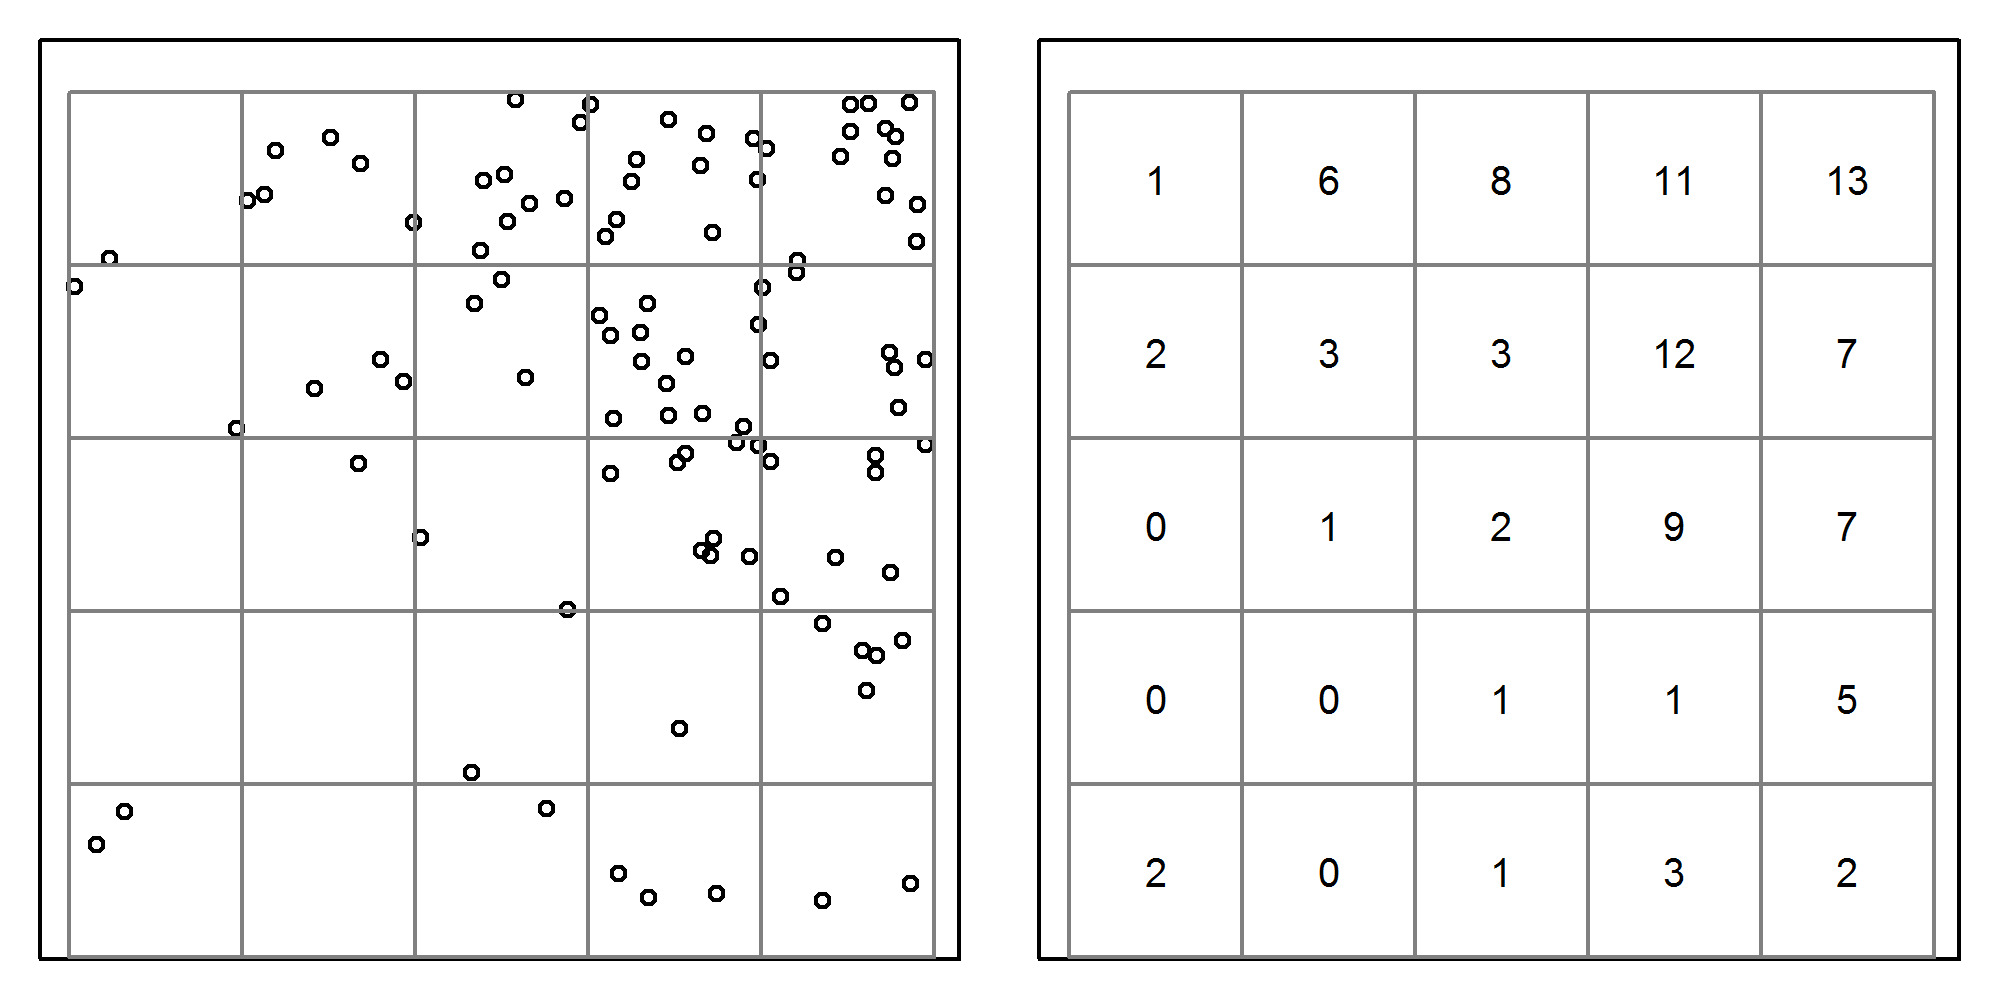
\includegraphics[width=5in,height=2.5in]{figs/heteroPlots}%{figs/elevMap}
\label{ch9:fig:elevMap}
\caption{An example of a spatial covariate, say elevation, and a
  realization of a inhomogeneous binomial point process with $N$=100
  and $\mu(x) = exp(\alpha Elev)$ where $\alpha=2$.}
\end{figure}

The simulated data are shown in Fig~\ref{fig:elevMap}. High elevations
are represented by light green and low elevations by dark green. The
activity centers of one hundred animals are shown as
points, and it is clear that these simulated animals prefer the high
elevations.  The underlying model describing this preference is
$\log(\mu(x)) = exp(\alpha \times Elevation(x))$
where $\alpha=2$ is the parameter to be estimated and $Elevation(x)$
is a function of the coordinates at $x$, as displayed on the map.

Given these points, we will now estimate $\alpha$ by minimizing the
negative-log-likelihood using \verb+R+'s \verb+optim+ function.

\begin{small}
\begin{verbatim}
# Negative log-likelihood
nll <- function(beta) {
  -sum(beta*cov(S[,1], S[,2]) - log(int2d(beta)))
  }
starting.value <- 0
fm <- optim(starting.value, nll, method="Brent",
            lower=-5, upper=5, hessian=TRUE)
c(Est=fm$par, SE=sqrt(1/fm$hessian)) # estimates and SEs
\end{verbatim}
\end{small}


Maximizing the likelihood took a small fraction of a second, and we
obtained an estimate of $\hat{\alpha}=2.01$. Not bad! We could plug in
this estimate to our linear model at each point in the state-space to
obtain the MLE for the intensity surface.

This example demonstrates
that if we had the data we wish we had, {\it i.e.} if we knew the
coordinates of the activity centers, we could easily estimate the
parameters governing the underlying point process. Unfortunately, in
SCR models, the activity centers cannot be directly observed, but
spatial re-captures, that is captures of individuals at
multiple locations in space, provide us with the information needed to
estimate these latent parameters.

\subsection{Fitting inhomogeneous point process SCR model}

One of the nice things about hierarchical models is that they allow us
to break a problem up into a series of simple conditional
relationships. Thus,
we can simply add the methods described above into our existing MCMC
algorithm to simulate the posteriors of $\alpha$ conditional on the
simulated values of $\mathbf{s}_i$. To demonstrate, we will continue with
the previous example. Specifically, we will overlay a grid of
traps upon the map shown in Fig.~\ref{ch9:fig:elevMap}. We will then
simulate capture histories conditional upon the activity centers shown
on the map. Then, we will attempt to estimate the activity center
locations as though we did not know where they were.


Here is some \verb+R+ code to simulate the encounter histories under a
Poisson observation model, which would be appropriate if animals could
be detected multiple times at a trap during a single occassion.

\begin{small}
\begin{verbatim}
# Create trap locations
xsp <- seq(-0.8, 0.8, by=0.2)
len <- length(xsp)
X <- cbind(rep(xsp, each=len), rep(xsp, times=len))

# Simulate capture histories, and augment the data
ntraps <- nrow(X)
T <- 5
y <- array(NA, c(N, ntraps, T))

nz <- 50 # augmentation
M <- nz+nrow(y)
yz <- array(0, c(M, ntraps, T))

sigma <- 0.1  # half-normal scale parameter
lam0 <- 0.5   # basal encounter rate
lam <- matrix(NA, N, ntraps)

set.seed(5588)
for(i in 1:N) {
    for(j in 1:ntraps) {
        distSq <- (s[i,1]-X[j,1])^2 + (s[i,2] - X[j,2])^2
        lam[i,j] <- exp(-distSq/(2*sigma^2)) * lam0
        y[i,j,] <- rpois(T, lam[i,j])
    }
}
yz[1:nrow(y),,] <- y # Fill
\end{verbatim}
\end{small}

Now that we have a simulated capture-recapture dataset $y$, and we have
augmented it to create the new data object $yz$, we are ready to
begin sampling from the posteriors. A commented Gibbs sampler written
in \verb+R+ is available online. There are two small parts of the
\verb+R+ code that distinguish it from previous code we have shown to
fit homogeneous point processes. First, we need to update the parameter
${\bf \alpha}$ conditional on all other parameters in the model. The code to
do so is:

\begin{small}
\begin{verbatim}
D1 <- int2d(beta1, delta=.05)
beta1.cand <- rnorm(1, beta1, tune[3])
D1.cand <- int2d(beta1.cand, delta=0.05)
ll.beta1 <- sum(  beta1*cov(S[,1],S[,2]) - log(D1) )
ll.beta1.cand <- sum( beta1.cand*(S[,1]+S[,2]) - log(D1.cand) )
if(runif(1) < exp(ll.beta1.cand - ll.beta1) )  {
    beta1<-beta1.cand
}
\end{verbatim}
\end{small}

Next, we need to put the new prior on the activity centers:

\begin{small}
\begin{verbatim}
#ln(prior), denominator is constant
prior.S <- beta1*cov(S[i,1], S[i,2]) # - log(D1)
prior.S.cand <- beta1*(Scand[1] + Scand[2]) # - log(D1)
if(runif(1)< exp((ll.S.cand+prior.S.cand) - (ll.S+prior.S))) {
    S[i,] <- Scand
    lam <- lam.cand
    D[i,] <- dtmp
    }
\end{verbatim}
\end{small}

Applying this modified sampler to our data we obtain posterior
distributions summarized in Table~\ref{tab:simIPP}. Mixing is good, and as usual,
life is very nice when we are working with simulated data.


\comment{

# MCCM code

source("thinSmcmc_exp.R")
ls()

fm1 <- scrIPP(yz, X, M, 3000, xlims=c(-1,1), ylims=c(-1,1),
            tune=c(0.002, 0.1, 0.25, 0.07) )

library(coda)
plot(mcmc(fm1$out))

rejectionRate(mcmc(fm1$out))



}



\begin{table}
\centering
\begin{tabular}{lccccc}
Parameter & Mean & SD  & q0.025 & q0.5 & q0.975 \\
\hline
$\alpha$    &&&&& \\
$\lambda_0$  &&&&& \\
$\sigma$    &&&&& \\
$N$        &&&&& \\
Density     &&&&& \\
\hline
\end{tabular}
\label{ch9:tab:simIPP}
\end{table}

It is worth noting that these models can also be fitted using
\verb+BUGS+ when the covariates are available in raster format. As
mentioned previously, we can define $s_i$ as the pixel id, and use the
categorical distribution as a prior.

\begin{verbatim}
s[i] ~ dcat(probs[])
mu[i] <- exp(alpha*covariate[i])
probs[k] = mu[i]/sum(mu[])
\end{verbatim}

A good example of this is in +cite{Kery capricaillie}. One must be
aware, however, that for larger rasters, computing the denominator
will be a ghastly slow process when done 50,000 times in MCMC, but
this seems to run faster using \verb+JAGS+ than in \verb+BUGS+.

[andy will have some stuff about this in Ch5]

Here is a cool example.


\begin{verbatim}



\end{verbatim}


\subsection{The jaguar data}

Estimating density of large felines was difficult before the advent of
SCR. This is because you would never be able to conduct a distance
sampling analysis for such rare and cryptic species, and because
traditional capture-recapture methods don't yield estimates of
density, only population size within some unknown region. This example
not only demonstrates how readily density can be estimated for a
globally imperilled species, but it also shows the importance of
estimating density rather than just population size.

[describe study]

A few aspects of this design are noteworthy. First, the dimensions and
configuration of the trap array differed among the regions of the trap
array. This fact alone could explain variation in the number of
animals exposed to sampling, which would have no biological
meaning. Furthermore, the area of inference is an irregular polygon
that was not sampled uniformly. Only by estimating density can we hope
to extrapolate our estiamates from the sampled region to get what we
are after. In this case, this is readily accomplished since the entire
state-space can be classified as one of the 3 levels of protection
from poaching. Of course, it general it is always preferable to sample
more uniformly throughout the area of interset in case some unmeasured
covariate biases the extrapolation.

To assess the influence of poaching on jaguar density, we considered 2
metrics of poaching pressure, one political and one continuous measure
of accessibility (Fig xxx).



\section{MLE}

Maybe its easy to adapt the MLE code from chapter 5 for doing a
spatial covariate? For completeness it might be worth having that.

\section{Other ideas}

Should have some discussion on some ideas for building flexible
models. Might be cool to use the Ickstadt/Wolpert as a model for the
inhomogeneous point process. Dont have to do it, just mention it. Also
some kind of a spline model or similar.




\section{Summary}

When state-space covariates are available, we can model
density by replacing the uniform prior on the activity centers with a
prior based on a log-linear function of covariates.





%\chapter{Modeling Encounter Probability}
%\label{chapt.covariates}

\chapter{Alternative Models for the Encounter Process}
\label{chapt.poisson-mn}

In the previous chapter we considered a very specific but not
terribly limited observation model. The observation model consisted of
two main elements: First a description of the encounter process
by which individuals are detected in traps. Specifically, we
assumed individual trap-specific encounters were iid Bernoulli
trials. The consequence of this is that individuals function
independently of one another and can be captured in
any number of traps during a specific interval of trapping
effort, but only 1 time per trap. 
The type of device is typical of bear hair snares, which we
considered as an example in that section. 
 It is natural to consider
alternative functional forms of this detection probability model which
we do in Chapt. \ref{chapt.covariates} and elsewhere.

In this chapter we consider alternative observation models which
accommodate Poisson or multinomial observation models. For example, if
sampling devices can detect an individual some arbitrary number of
times during an interval, then it is natural to consider observation
models for encounter frequencies, such as the Poisson model. Another
type of encounter device is the ``multi-catch'' device
\citep{efford_etal:2009euring} which
is a physical device that can capture and hold an arbitrary number of
individuals. A typical example is a mist-net for birds
\citep{borchers_efford:2008}.  It is natural to regard observations
from these kinds of studies as independent multinomial observations.
A related type of device that produces {\it dependent} multinomial
observations are the so-called {\it single-catch} traps
\citep{efford_etal:2009euring}. The canonical example are small-mammal
live traps which catch and hold a single individual. Competitation
among individuals for traps induces a complex dependence structure
among individual encounters. To date, no formal inference framework
has been devised for this method although it stands to reason that the
independent multinomial model should be a good approximation in some
situations \citep{efford_etal:2009euring}.  There are other
observation systems that we discuss here.

One thing that is apparent from our development of the multinomial
observation model is that SCR models are a kind of multi-state model,
in the conventional sense as applied in capture-recapture studies. In
the context of SCR though, the ``state'' variable is a geographic
location and the transition probabilities are parameterized by
distance between the states.





\section{Poisson Observation Model}

The models we analyze in Chapt. \ref{chapt.scr0} assumed binary
observations -- i.e., standard encounter history data -- so
that individuals are captured at most one time in a trap.  This makes
sense for many types of DNA sampling (e.g., based on hair snares)
because distinct visits to sampled locations or devices cannot be
differentiated. However, many encounter methods or devices make it
possible to encounter an individual some arbitrary number of times
during any particular sampling episode XXXX EFFORD CITE XXXXXX. 
That is, we might observe
encounter frequencies $y_{ijk}>1$
for individual $i$, trap $j$ and
sampling interval $k$.  As an example, if a camera device is
functioning properly it may be programmed to take photos every few
seconds if triggered.  For a second example, suppose we are searching
a quadrat or length of trail for scat, we may find multiple samples from the same
individual.
Therefore, we seek observation models that accommodate such encounter
frequency data.  In general, any discrete probability mass function
could be used for this purpose, including the standard models for
count data used throughout ecology, the Poisson and negative
binomial.  Here we focus on using the Poisson
model only although other count frequency models are possible XXX
EFFORD ciTE XXXX.

Let $y_{ijk}$ be the frequency of encounter for
individual $i$, in trap $j$, during occasion $k$, then assume:
\[
 y_{ijk} \sim \mbox{Poisson}(\lambda_{ij})
\]
where the expected encounter frequency $\lambda_{ij}$ depends on both
individual and trap. As we did in the binary model of
Chapt. \ref{chapt.scr0}, we
now seek to model the expected value of the observation (which was
$p_{ij}$ in Chapt \ref{chapt.scr0}) as a function of the individual activity center
${\bf s}_{i}$.
We propose
\[
 \lambda_{ij} = \lambda_{0}  g({\bf x}_{j},{\bf s}_{i})
\]
Where $g({\bf x},{\bf s})$ is any positive valued function, such as
the negative exponential or the bivariate Gaussian kernel.
Then $\lambda_{0}g({\bf x},{\bf s})$ is the expected encounter rate in trap
${\bf x}$ for an individual having activity center ${\bf s}$.  Note
that
\[
 log(\lambda_{ij}) = log(\lambda_{0}) + log(  g({\bf x}_{j},{\bf
   s}_{i}) )
\]
where, if we set $\alpha_{0} \equiv log(\lambda_{0})$, and, if 
$g({\bf x},{\bf s}) \equiv exp(-\alpha_{1} d({\bf x},{\bf s})^2)$
(i.e., the Gaussian model), then:
\begin{equation}
 log(\lambda_{ij}) = \alpha_{0} + \alpha_{1} d({\bf x}_{j},{\bf s}_{i})^{2}
\label{poisson-mn.eq.lp}
\end{equation}
which is the same linear predictor as we have seen for the Bernoulli
model in Chapt. \ref{chapt.scr0}.  We can accommodate covariates at
the level of individual-, trap- or sample occasion by including them
on the baseline encounter rate parameter $\lambda_{0}$. For example,
if $C_{j}$ is some covariate that depends on trap only, then we have:
\[
log(\lambda_{0,ijk}) = \alpha_{0} + \alpha_{2} C_{j}
\]
and therefore covariates on the logarithm of baseline encounter
probability appear also as linear effects on $\lambda_{ij}$.  We don't
get into too much discussion of general covariate models here, but see
Chapt. \ref{chapt.covariates} for a more comprehensive development of
such models along with examples. 


For a  model in which we have covariates that vary across
the sample occasions  $k$, we can aggregate the observed data by the
property of compound additivity of the Poisson distribution (if $x$ and
$y$ are $iid$ Poisson with mean $\lambda$ then $x+y$ is Poisson with
mean $2\lambda$). Therefore,
\[
y_{ij} = (\sum_{k=1}^{K} y_{ijk}) =  \mbox{Poisson}(K  \lambda_{0}
g({\bf x}_{j},{\bf s}_{i}) )
\]
We see that $K$ and $\lambda_{0}$ serve the same role as affecting the
base encounter rate. Since the observation model is the same,
probabilistically speaking, for all values of $K$, evidently we need
only $K=1$ ``survey'' from which to estimate model parameters. We know
this intuitively as sampling by multiple traps serves as replication
in SCR models.

\subsection{Poisson model of space usage}

How do we interpret this model?  A natural interpretation of the
encounter process model is that resulting from movement of individuals
about their home range (sec. \ref{scr0.sec.implied}).  Imagine we have
perfect samplers in every pixel of the landscape that discharge at set
time intervals (e.g., every hour), and let $m_{ij}$ be the number of
times individual $i$ was recorded in pixel $j$. For pure model of
space usage, we might think of this model:
\[
m_{ij} \sim  \mbox{Poisson}(K  g({\bf x}_{j},{\bf s}_{i}) )
\]
where $K$ is the number of time intervals recorded. This model of
space usage gives rise to the standard resource selection function
(RSF) models \citep[][and Chapt. \ref{chapt.rsf}]{royle_etal:2012mee}.
But now suppose our samplers are not perfect but, rather, record only
a fraction of the resulting visits. A sensible model is
\[
 y_{ij}|m_{ij} \sim \mbox{Bin}(m_{ij}, \lambda_{0}).
\]
The marginal distribution of $y_{ij}$ is:
\[
 y_{ij} \sim \mbox{Poisson}(K \lambda_{0} g({\bf x}_{j},{\bf s}_{i}) ).
\]
Therefore, we see that encounters accumulate in proportion to the
frequency of outcomes of an individual using space (or ``selecting
resources'').

We introduced this interpretation of the model in terms of movement
and space usage in sec. \ref{scr0.sec.implied}, and it is one of the
main underlying concepts of SCR models that is not present in ordinary
capture-recapture models. As we noted previously, the underlying model
of space usage is only as complex as the encounter probability (or
rate) model which is, so far, only symmetric and stationary (does not
vary in space). 




\subsection{Poisson relationship to the Bernoulli model}

There is a sense in which the Poisson and Bernoulli models can
be viewed as consistent with one another. Note that under the Poisson
model with $E(y) = \lambda$ we have:
\begin{equation}
 \Pr(y>0) = 1-exp(-\lambda)
\label{eq.cloglog}
\end{equation}
Therefore, if we equate the event ``encountered'' with the event that
the individual was captured at least 1 time under the Poisson model,
i.e., $y>0$, then it would be natural to set $p_{ij} = \Pr(y>0)$
according to \ref{eq.cloglog}.

In fact, as $\lambda$ gets small, the Poisson model is a close approximation
to the Bernoulli model in the sense that outcomes concentrate on
$\{0,1\}$, i.e.,  $\Pr(y\in \{0,1\})
\rightarrow 1$ as $\lambda \rightarrow 0$.
A relevent property of the Poisson model
is that
$\Pr(y>0) \rightarrow \lambda$
for small values of $\lambda$.
This phenomenon is shown in  Fig.
\ref{poisson-mn.fig.poissonbern} where
the left panel shows a plot of $\lambda_{ij}=\lambda_{0}g({\bf
  x}_{j},{\bf s}_{i};\sigma)$ vs. distance and
superimposed on that is a plot of $p_{ij}=1-exp(-\lambda_{ij})$ vs. distance, for values
$\lambda_{0} = .1$ and $\sigma = 1$, and the right panel shows a plot of
$\Pr(y>0)$ vs. $E[y]$. We see that the two quantities are
practically indistinguishable.

This is
convenient in some cases because the Poisson model might be more
tractable to fit (or even vice versa). For an example, see the models
described in Chapt. \ref{chapt.scr-unmarked}, and we also consider
another case in sec. \ref{poisson-mn.sec.singlecatch} below. To
evaluate the closeness of the approximation, you can use the following
{\bf R} commands which we used to produce
Fig. \ref{poisson-mn.fig.poissonbern}:
{\small
\begin{verbatim}
x<-seq(0.001,5,,200)
lam0<- .1
sigma<- 1
lam<- lam0*exp(-x*x/(2*sigma*sigma))

par(mfrow=c(1,2))
p1<- 1-exp(-lam)
plot(x,lam,ylab="E[y] or Pr(y>0)",xlab="distance",type="l",lwd=2)
lines(x,p1,lwd=2,col="red")
plot(lam,p1,xlab="E[y]",ylab="Pr(y>0)",type="l",lwd=2)
abline(0,1,col="red")
\end{verbatim}
}

To summarize, if $y$ is Poisson and, as $\lambda$ gets small,
\begin{eqnarray*}
\Pr(y>0)  & \approx & E[y]  \\
1-exp(-\lambda_{0} g(x,s)) &\approx &  \lambda_{0} g(x,s)
\end{eqnarray*}
which explains the close correspondance we have found between these
two versions of the Gaussian encounter probability model (sec. \ref{scr0.sec.implied}).
What all of this suggests it that
if we see very few observations $>1$ then we wont lose much
information by using the Bernoulli model. On the other hand, the
Poisson model may have some advantages in terms of analytic or numerical
tractability in some cases.

\begin{figure}
\centering
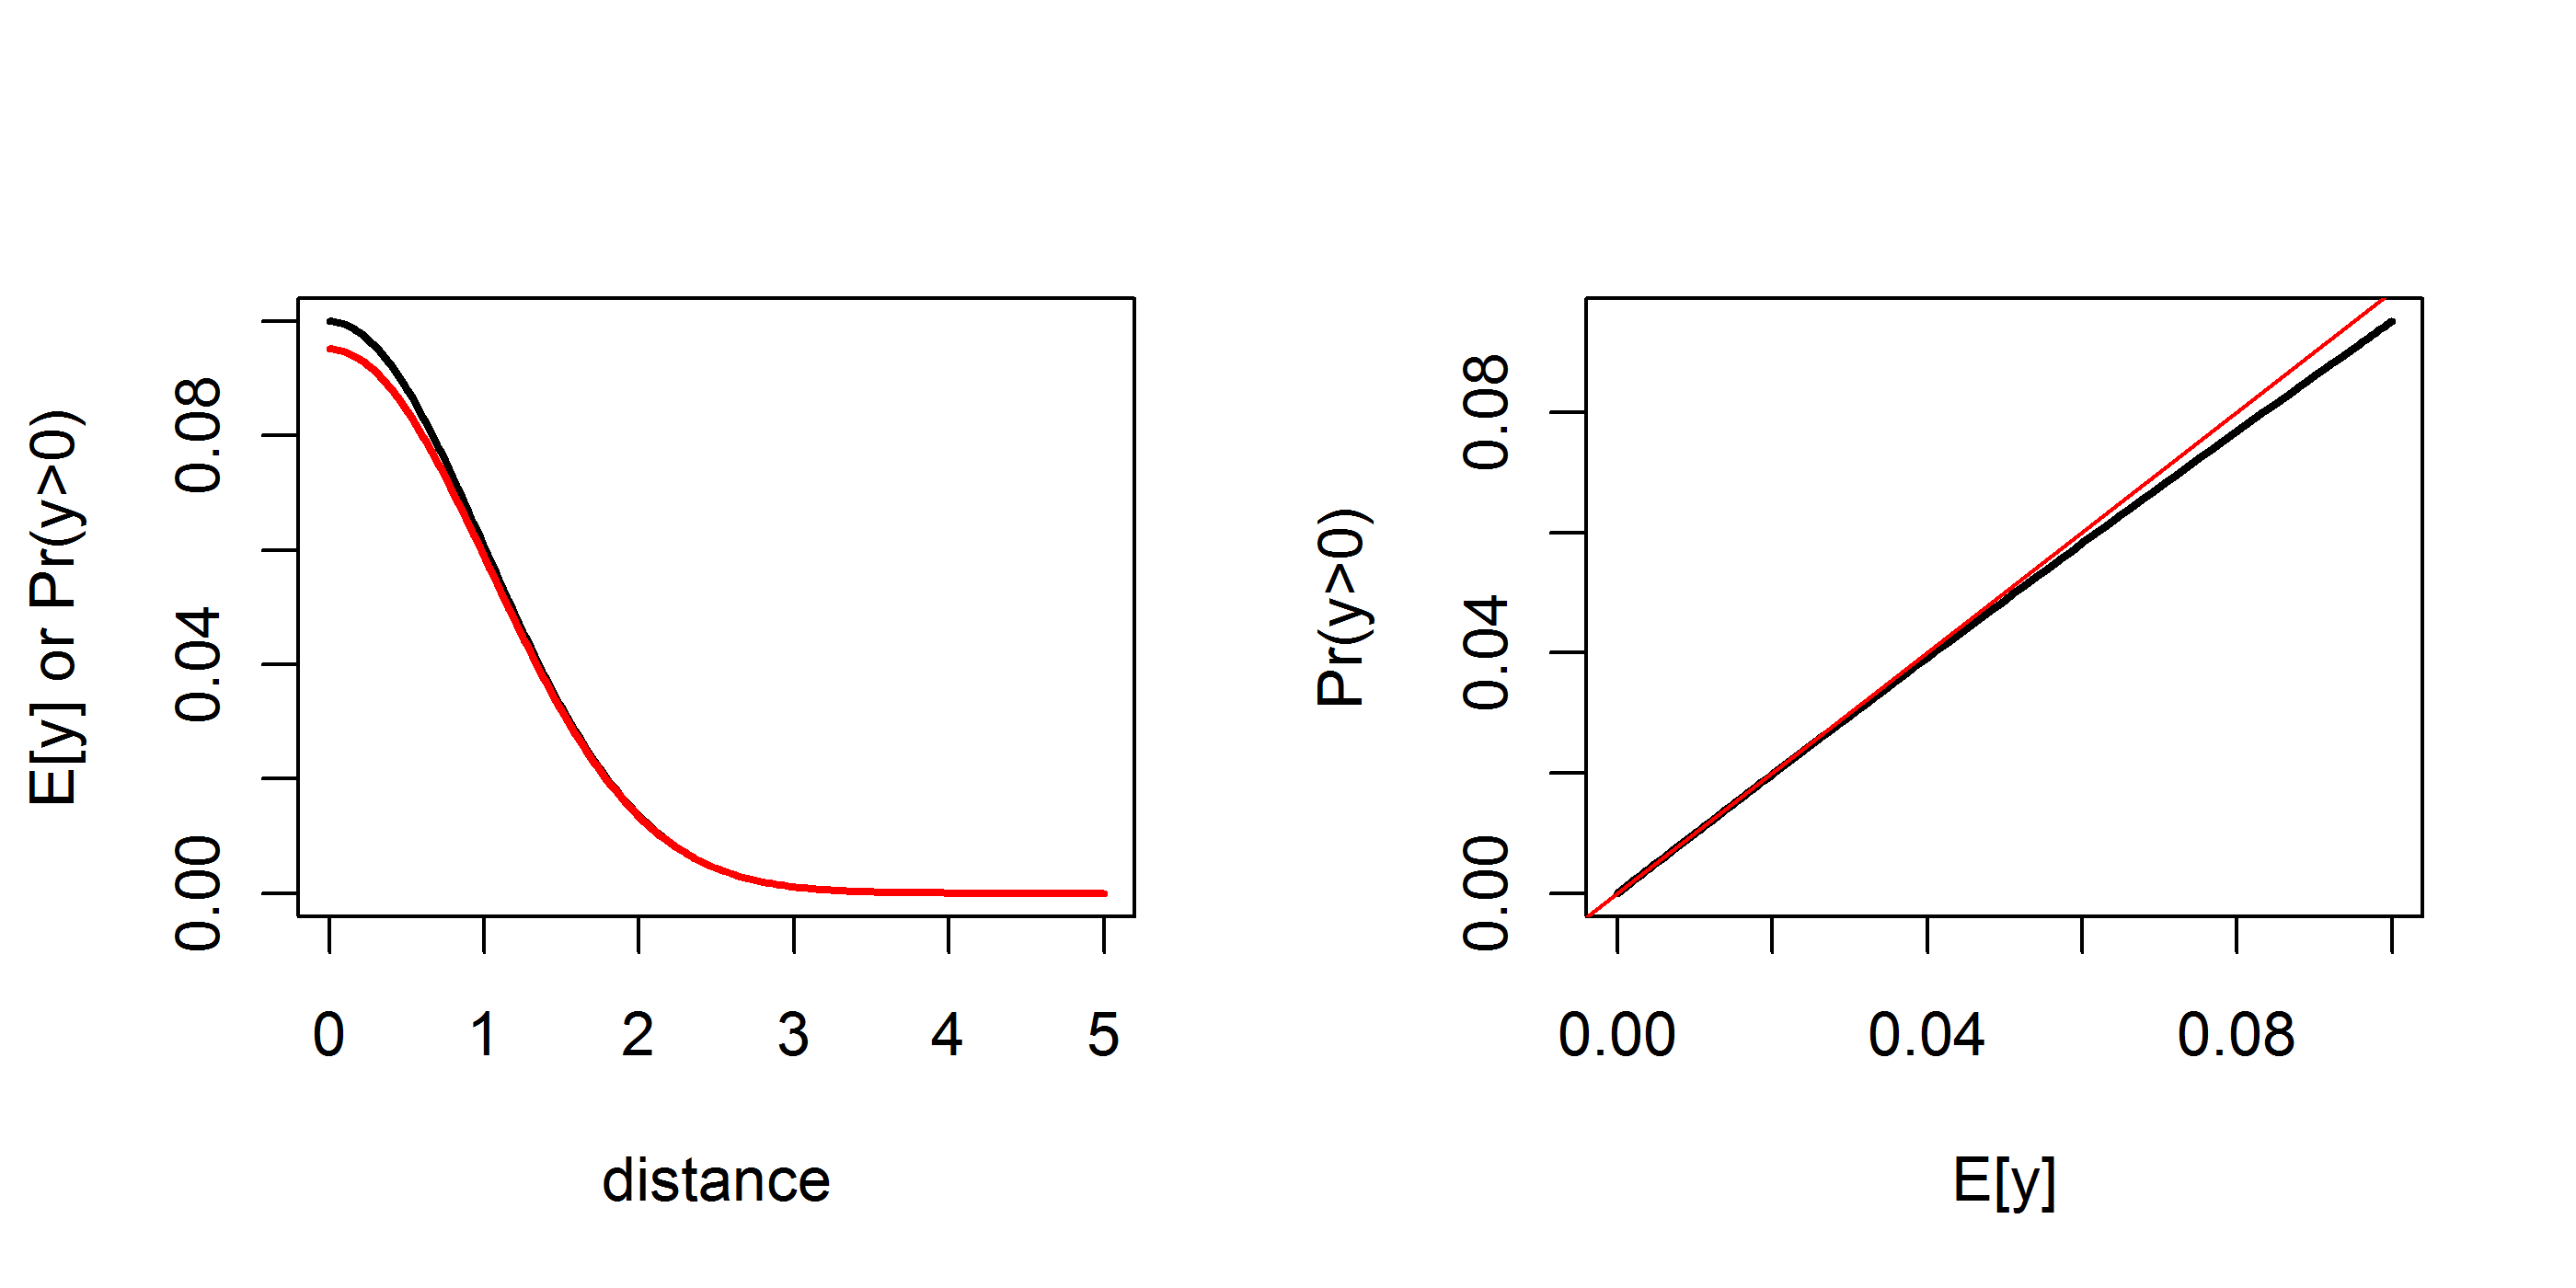
\includegraphics[width=5in,height=2.5in]{Ch5-PoisMn/figs/Poisson-Bern.png}
\caption{Poisson approximation to the binomial. As the Poisson mean
  approaches 0, then $Pr(y>0)$ under the Poisson model approaches
  $\lambda$ and therefore $y \sim Poisson$ is well-approximated by a
  Bernoulli model with parameter $\lambda$.
}
\label{poisson-mn.fig.poissonbern}
\end{figure}

Even in such cases where we're not in the range where the Poisson and
Bernoulli models are nearly equivalent,
we might choose to truncate  individual encounter frequencies
to binary observations anyhow (``quantize'').
We might do
this intentionally, but sometimes this truncation is a feature of the
sampling. For example, in the case of bear hair snares, the number of
encounters might be well approximated by a Poisson distribution but we
cannot determine unique visits and so only get to observe the binary
event ``$y>0$''. Similarly for scat sampling problems it will not
generally be possible to diagnose distinct ``independent'' scat
samples. Under this model the data are only binary encounters and we
might therefore choose a model of the form:
\[
\mbox{ cloglog}(p_{ij}) = \log(\lambda0)  + \log(g({\bf x},{\bf s}))
\]
\begin{comment}
This example shows us that the choice of link function is typically
directly related to a specific encounter frequency model and,
furthermore, the choice of link function is equivalent to choice of
``detection function.''
%As another example, what if the latent
%encounter frequencies are actually geometric random variables where
%the mean is a function of distance? For the case where the support of
%y includes 0 – so that $y$ is the number of failures before the 1st
%success, then the mean is $\mu = (1-p)/p$.  $Pr(y>0) =$ ??
%\[
%logit() = ….?
%\]
\end{comment}

\subsection{A cautionary note on modeling encounter frequencies}

Other models for counts might be appropriate. For example, ecologists
are especially fond of negative binomial models for count data
\citep{verhoef_boveng:2007,white_bennetts:1996,kery_etal:2005}
but other models for excess-Poisson variation are possible. For
example, we might add a normally distributed random effect to
the linear predictor.

As a general rule we favor the Bernoulli observation model even if
encounter frequencies are obtained by sampling.  The main reason is
that, with frequency data, we are forced to confront a model choice
problem (i.e., Poisson, negative binomial, log-normal mixture) that is
wholly unrelated to the fundamental space usage process that underlies
the genesis of SCR data. Repeated encounters over short time intervals
are not likely to be the result of independent encounter
processes. E.g., an individual moving back and forth in front of a
camera yields a cluster of observations that is not informative about
the spatial structure of the model. Similarly in scat surveys (e.g.,
Thompson et al. in review), dogs are used to locate scats which are
processed in the lab for individuality.  The process of local scat
deposition is not really the outcome of movement or space usage but rather the
outcome of complex behavioral considerations as well as dependence in
detection of scat by dogs. E.g., they find one and then more likely to
find a nearby one, or they get into a den area and find lots of scats.
This additional model assumption required to model variation in
observed frequencies (i.e., conditional on location) provides
relatively no information about density, and we feel that the
model selection issue should therefore be avoided.

To elaborate on this, it seems natural to construct models for
encounter data that are conditional on movement outcomes: We suppose
that an individual visits a particular pixel ${\bf x}$ with some probability
$p({\bf x}, {\bf s})$,
 and then, once its
there, deposits a
number of scat, or visits a camera some number of times with frequency
$y(x,s) \ge 0$.
We describe the outcome of this movement/usage with
a two-level hierarchical model of the form:
$[y|z][z|p({\bf x},{\bf s})]$.
Let $z({\bf x},{\bf s})$ be a binary variable
that indicates whether the individual with activity center ${\bf s}$
visits pixel ${\bf x}$ during some interval, and let
$z({\bf x},{\bf s}) \sim  \mbox{Bern}(p({\bf x},{\bf s}))$ and
suppose
 the encounter frequency $y$ is independent of ${\bf x}$ and
${\bf s}$ conditional
on the binary event $z$,  that the individual visited pixel $x$.
Therefore, the model for $y$ (amount of use) does not
depend on ${\bf s}$.

\begin{comment}
Moreover, consideration of encounter frequency data could lead to
important identifiability problems along the lines of \citet{link:2003}. The
basic Poisson model can be over-dispersed in a number of ways to
produce different models of over-dispersion.  i.e., gamma noise,
normal noise, exponential noise, etc..  Thus we have different models
of heterogeneity, analogous to the class of models considered by
\citet{link:2003},
\end{comment}

\section{Analysis of the Poisson SCR model in BUGS}

We consider the simplest possible model here in which we have no
covariates that vary over sample occasions  $k=1,2,\ldots,K$ 
so that we work with
the aggregated individual- and trap-specific encounters:
\[
y_{ij} = (\sum_{k=1}^{K} y_{ijk}) =  \mbox{Poisson}(K  \lambda_{ij})
\]
We consider a bivariate normal form of $g({\bf x}_{j},{\bf s}_{i})$ so
that
\[
g({\bf x}_{j},{\bf s}_{i}) = exp( -d({\bf x}_{j}, {\bf
  s}_{i})^{2} /(2\sigma^{2}))
\]
so that 
\[
log( \lambda_{ij})  =\alpha_{0} + \alpha_{1} d({\bf x}_{j}, {\bf s}_{i})^2
\]
where $\alpha_{0} = log(\lambda_{0})$ and $\alpha_1 = 1/(2\sigma^2)$.


As usual, we approach Bayesian analysis of these
models using data augmentation (sec. \ref{closed.sec.da}).
Under data augmentation, we introduce a collection of all-zero encounter
histories to bring the total size of the data set up to $M$, and a corresponding
set of data augmentation variables $z_{i} \sim \mbox{Bern}(\psi)$. Then
the observation model is specified conditional on $z$ according to:
\[
y_{ij} \sim  \mbox{Poisson}(z_{i} K  \lambda_{ij})
\]
which evaluates to a point mass at $y=0$ if $z=0$.  In other words, the
observation model under data augmentation is a zero-inflated Poisson
model which is easily analyzed by Bayesian methods, e.g., in one of
the {\bf BUGS}
dialects, or  using likelihood methods, which we neglect here although
the same principles as in Chapt. \ref{chapt.mle} apply.


\subsection{Simulating Data and Fitting the Model}


Simulating a sample SCR data set under the Poisson model requires only
a couple minor modifications to the procedure we used in
Chapt. \ref{chapt.scr0}. In
particular, we modify the block of code which defines the model to be
that of $E(y)$ and not $\Pr(y=1)$, and we change the random variable
generator from \mbox{\tt rbinom} to \mbox{\tt rpois}:
{\small
\begin{verbatim}
D<- e2dist(S,traplocs)

alpha0<- -2.5
sigma<- 0.5
alpha1<- 1/(2*sigma*sigma)

muy <-  exp(alpha0)*exp(-alpha1*D*D)
# now generate the encounters of every individual in every trap
Y<-matrix(NA,nrow=N,ncol=ntraps)
for(i in 1:nrow(Y)){
 Y[i,]<-rpois(ntraps,K*muy[i,])
}
\end{verbatim}
}

We modified our simulation code from Chapt. \ref{chapt.scr0} to
simulate Poisson encounter frequencies for each trap and then we
analyze an ideal data set using {\bf BUGS}. The new function,
available in the \mbox{\tt scrbook} package, is called {\tt
  simPoissonSCR.fn}.  The simulator can produce 3-d encounter history
data too although we don't do that here.  Here is an example of
simulating a data set and harvesting the required data objects, and
doing the data augmentation:

{\small
\begin{verbatim}
data<-simPoissonSCR.fn(discard0=TRUE,sd=2013)
y<-data$Y
traplocs<-data$traplocs
nind<-nrow(y)
X<-data$traplocs
K<-data$K
J<-nrow(X)
Xl<-data$xlim[1]
Yl<-data$ylim[1]
Xu<-data$xlim[2]
Yu<-data$ylim[2]

## Data augmentation stuff
M<-200
y<-rbind(y,matrix(0,nrow=M-nind,ncol=ncol(y)))
z<-c(rep(1,nind),rep(0,M-nind))
\end{verbatim}
}

The process for fitting
the model in \winbugs  or \jags is identical to what we've done
previously in Chapt. \ref{chapt.scr0}. In particular, we set up some
starting values, package the data and inits, identify the parameters
to be monitored, and then send everything off to our MCMC engine. Here
it all is for fitting the Poisson observation model (these commands
are shown in the help file for \mbox{\tt simPoissonSCR.fn}):

{\small
\begin{verbatim}
sst<-traplocs[sample(1:J,M,replace=TRUE),] # starting values for s
for(i in 1:nind){
if(sum(y[i,])==0) next
sst[i,1]<- mean( X[y[i,]>0,1] )
sst[i,2]<- mean( X[y[i,]>0,2] )
}
sst<-sst + runif(nrow(sst)*2,0,1)/8
data <- list (y=y,X=X,K=K,M=M,J=J,Xl=Xl,Yl=Yl,Xu=Xu,Yu=Yu)
inits <- function(){
  list (alpha0=rnorm(1,-2,.4),alpha1=runif(1,1,2),s=sst,z=z,psi=.5)
}
parameters <- c("alpha0","alpha1","N","D")

cat("
model {
alpha0~dnorm(0,.1)
alpha1~dnorm(0,.1)
psi~dunif(0,1)

for(i in 1:M){
 z[i] ~ dbern(psi)
 s[i,1]~dunif(Xl,Xu)
 s[i,2]~dunif(Yl,Yu)
for(j in 1:J){
d[i,j]<- pow(pow(s[i,1]-X[j,1],2) + pow(s[i,2]-X[j,2],2),0.5)
y[i,j] ~ dpois(lam[i,j])
lam[i,j]<- z[i]*K*exp(alpha0)*exp(- alpha1*d[i,j]*d[i,j])
}
}
N<-sum(z[])
D<- N/64
}
",file = "SCR-Poisson.txt")

nthin<-1; nc<-3; nb<-1000; ni<-2000

library("R2WinBUGS'')
out1 <- bugs (data, inits, parameters, "SCR-Poisson.txt", n.thin=nthin,n.chains=nc,
 n.burnin=nb,n.iter=ni,working.dir=getwd(),debug=TRUE)
\end{verbatim}
}
{\flushleft Or using {\bf JAGS}  we do this instead: }
{\small
\begin{verbatim}
library(rjags)
fm <- jags.model("SCR-Poisson.txt", data=data, inits=inits, n.chains=nc, n.adapt=nb)
out2 <- coda.samples(jm, parameters, n.iter=ni, thin=nthin)
\end{verbatim}
}
{\flushleft 
Summarizing } the output from the {\bf WinBUGS}  run produces the following:
{\small
\begin{verbatim}
> print(out1,digits=2)
Inference for Bugs model at "SCR-Poisson.txt", fit using WinBUGS,
 3 chains, each with 2000 iterations (first 1000 discarded)
 n.sims = 3000 iterations saved
           mean    sd   2.5%    25%    50%    75%  97.5% Rhat n.eff
alpha0    -2.57  0.19  -2.95  -2.69  -2.57  -2.44  -2.19 1.00  2600
alpha1     2.34  0.36   1.69   2.08   2.32   2.57   3.12 1.00  3000
N        114.13 15.25  87.97 103.00 113.00 124.00 147.00 1.01   370
D          1.78  0.24   1.37   1.61   1.77   1.94   2.30 1.01   370
deviance 329.95 21.92 290.00 314.20 329.50 344.40 375.80 1.00  1700

...
[..some output deleted..]
...
\end{verbatim}
}

%We don't provide a real example of a Poisson SCR model here although
%we use this observation model for an analysis of some data in Chapt.
%\ref{chapt.searchencounter}. {\bf XXXX DO WE DO THIS ANYWHERE? XXXXX}

\begin{comment}
\subsection{Exercise}

Use the Bernoulli model simulator from Chapt. \ref{chapt.scr0} (\mbox{\tt
  simSCR0.fn}) to simulate a Bernoulli data set and then fit the
Poisson model. Compare the results of fitting the correct
data-generating model with those of fitting the misspecified Poisson
model.
\end{comment}


\section{Analysis of the Wolverine Study Data}

We reanalyzed the data from
the  wolverine camera trapping study that were first introduced in 
sec. \ref{chapt.scr0.wolverine}.
We modified the {\bf R} script from the function \mbox{\tt wolvSCR0.fn} to fit the
Poisson model (see the help file for \mbox{\tt
  wolvSCR0pois.fn}). Executing this function produces the following
results which are provided here:
{\small
\begin{verbatim}
Inference for Bugs model at "modelfile.txt", fit using WinBUGS,
 3 chains, each with 6000 iterations (first 1000 discarded)
 n.sims = 15000 iterations saved
           mean    sd   2.5%    25%    50%    75%  97.5% Rhat n.eff
psi        0.30  0.07   0.19   0.25   0.30   0.34   0.45    1   650
sigma      0.64  0.06   0.54   0.60   0.64   0.68   0.76    1   730
lam0       0.06  0.01   0.04   0.05   0.06   0.06   0.08    1  5000
logp0     -2.89  0.17  -3.22  -3.00  -2.89  -2.78  -2.57    1  5000
N         60.12 11.91  40.00  52.00  59.00  68.00  87.00    1   630
D          5.80  1.15   3.86   5.01   5.69   6.55   8.39    1   630
beta       1.24  0.21   0.86   1.10   1.23   1.38   1.69    1   730

...
[some output deleted]
...
\end{verbatim}
}
The results are almost indistinguishable from the Bernoulli model
fitted preveiously, where we had a posterior mean for $N$ of
 $59.84$,  $\sigma$ it was
$0.64$. The {\bf R} 
script is provided in the  \mbox{\tt scrbook} package which you can
use to modify the model or obtain more posterior samples for this model.
%In addition we did a basic assessment of Goodness-of-fit using a
%Bayesian p-value and statistic 1 as described in sec. XXXXX.  


\begin{comment}
\section{Likelihood analysis of the Poisson model}

Counts are Poisson with a random effect so this is stupidly easy to
implement.
We do the normal ``full likelihood'' approach in which we retain $N$
as a real parameter in the model. We adapt \mbox{\tt intlik3} from
chapter 5 here..... behold:

Poisson(lambda(s,x))

data augmentation = ZIP
\begin{verbatim}
Pr(yi) =   ( prod_{j} dpois(y) ) *psi + I(y=0)*(1-psi)

Actually if y(i,j) = Poisson( lambda(i,j) ) then we can just add up
sum_{j} y(i,j) =  Poisson( sum_{j} lambda(i,j)) right?

 int_{s} thatthing

Zero-inflate the result
\end{verbatim}
\end{comment}



\section{Independent Multinomial Observations}

Several types of encounter devices yield multinomial observations in
which an individual can be caught in a single trap during a particular
encounter occasion.  Mist nettting is the prime example -- these are
``multi-catch'' traps \citep{efford_etal:2009euring}. Also some kinds of
bird or mammal traps hold multiples of animals,
and pit-fall traps are commonly used for many types of
herptiles. These sampling methods are multi-catch devices.
Another important multi-catch method is area-searches of reptiles (or
any animal scat) where we think of
a small polygon as the ``trap'' -- we could get multiple individuals
(turtles, lizards) in the same plot but not, in the same sample
session, at different plots.  The key feature is that capture of an
individual in a trap is {\it not} independent of capture in other
traps, because once they are captured in a trap,
they can't be captured in any other trap.
On the
other hand, individuals behave independently of one another, or so it
might be reasonable to assume, so whether a trap captures some other
individual doesn't have bearning on whether it captures another.  This
last assumption is violated in an extreme case in classical ``single
catch'' traps which we address in sec. \ref{poisson-mn.sec.singlecatch}
below. In general we could imagine non-independence being important in
any multi-catch situation but to the best of our knowledge a general
model that encompasses complete dependence (single catch) and complete
independence (multi-catch) of individuals has not been proposed.  So
we treat the cases individually and, in this section, we address the
multi-catch situation wherein individuals behave independently.


In this case we regard the observation ${\bf y}_{ik}$ for
individual $i$ during sample occasion $k$ as a multinomial observation
which consists of a sequence of 0's and at most a single 1 indiciating
the trap of capture. For example, if we capture an individual in trap
2 during a 6 sample period study then ${\bf y}_{i} = (0,1,0,0,0,0)$.
If we sample for 5 periods in all and the individual is also caught
in trap 4 during sample 3, but otherwise uncaptured, then the 5 encounter observations for that
individual are as follows:
\begin{verbatim}
sample |---- trap ---------|
       1   2   3   4   5   6
 1     0   1   0   0   0   0
 2     0   0   0   0   0   0
 3     0   0   0   1   0   0
 4     0   0   0   0   0   0
 5     0   0   0   0   0   0
\end{verbatim}
Statistically we regard the {\it rows} of this data matrix as {\it
  independent} multinomial trials.

Analogous to our previous Bernoulli and Poisson models, we seek to
construct the multinomial cell probabilities for each individual, as a
function of {\it where} that individual lives, through its center of
activity ${\bf s}$. Thus we suppose that
\begin{equation}
 {\bf y}_{ik}|{\bf s}_{i} \sim \mbox{Multinom}(1, {\bm \pi}({\bf s}_{i}) )
\label{poisson-mn.eq.mn}
\end{equation}
where ${\bm \pi}({\bf s}_{i})$ is a vector of length $J+1$, which, by
convention here, we define $\pi_{i,J+1}$, the last cell, or the ``zero
cell'', to correspond to the event ``not captured''.
Now we have to
construct these cell probabilities in some meaningful way that depends
on each individuals' ${\bf s}$.
We use the standard
multinomial logit with distance as a covariate:
\[
 \pi_{ij} = \frac{  exp(\alpha_{0} - \alpha_{1} d_{ij}) }{ 1+ \sum_{j}
   exp(\alpha_{0} - \alpha_{1} d_{ij})}
\]
for $j=1,2,\ldots,J$ and, for $J+1$, i.e., ``not captured'',
\[
 \pi_{i,(J+1)} = \frac{  exp(0) }
                    { 1+ \sum_{j} exp(\alpha_{1} d_{ij})}
\]
or, more commonly, we use $d_{ij}^{2}$ to correspond to our Gaussian
kernel model for encounter probability.

A statistically equivalent distribution is the {\it categorical}
distribution.  If ${\bf y}$ is a multinomial trial with probabilities
${\bm \pi}$ than the {\it position} of the non-zero elemment of ${\bf
  y}$ is a categorical random variable with probabilities ${\bm \pi}$.
We express this as
\[
{\bf y}|{\bf s} \sim \mbox{Categorical}( {\bm \pi} )
\]
In the context of SCR models the categorical version of the
multinomial trial corresponds to the {\it trap of capture}.  Using our
example above with 6 traps then ${\bf y}_{i1} = (0,1,0,0,0,0)$ then we
could as well say $y_{ik}$ is a categorical random variable with
state-space (possible outcomes) $(1,2,3,4,5,6,7)$ where outcome $y=7$
corresponds to ``not captured.'' Obviously, how this is organized or
labeled is completely irrelevant, although it is convenient to use the
integers $1:(J+1)$) where $J+1$ is the event not captured.  Therefore,
for our illustration in the previous table, $y_{i1} = 2$, $y_{i2} =
7$, $y_{i3} = 4$ and so on.

For simulating and fitting data in the \bugs engines we will typically use
the categorical representation of the model because it is somewhat
more convenient.  We have found that fitting multinomial models in
{\bf WinBUGS} is less efficient than {\bf JAGS}
\citep{converse_royle:2013}, which we use in the subsequent examples
involving multinomial 
observation models.



\subsection{Simulating data and analysis using JAGS}

We're going to show the nugget of a simulation function which is
used in the function \mbox{\tt sim.mnSCR} found in the {\bf R} package
\mbox{\tt scrbook}.  The first lines of the following {\bf R} code
make use of some things that should be defined but we omit them here:
{\small
\begin{verbatim}
S<-cbind(runif(N,Xl,Xu),runif(N,Yl,Yu))
# how far is each individual from each trap?
D<- e2dist(S,traplocs)

# paramter values
sigma<- 0.5
alpha0<- -1
alpha1<- 1/(2*sigma*sigma)

# make an empty data matrix and fill it up
Ycat<-matrix(NA,nrow=N,ncol=K)
for(i in 1:N){
for(k in 1:K){
lp<- alpha0 - alpha1*D[i,]*D[i,]
cp<- exp(c(lp,0))
cp<- cp/sum(cp)
Ycat[i,k]<- sample(1:(ntraps+1),1,prob=cp)
}
}
\end{verbatim}
}
The resulting data matrix in this case has the maximal dimension $N$
and so, for analysis, to mimic a real situation, we would have to
discard the uncaptured individuals.  \mbox{\tt simMnSCR.fn} will also
simulate data that includes a behavioral response, which will be the
typical situation in small-mammal trapping problems, which we first
developed this code to deal with \citep[see][for
details]{converse_royle:2012}.

Here we use our function \mbox{\tt simMnSCR.fn} to simulate a data set
with $K=7$ periods, etc.. We'll run the model using \jags which
we have found is much more effective for this class of models.  We get
the data set-up for analysis by augmenting the size of the data set to
$M=200$. In addition we choose starting values for ${\bf s}$ and the
data augmentation variables $z$.  For ${\bf s}$ here we cheat a little
bit and use the true values for the obseved individuals and then
augment the matrix ${\bf S}$ with $M-n$ randomly selected activity
centers.

{\small
\begin{verbatim}
set.seed(2013)
parms<-list(N=100,alpha0= -.40, alpha2= 0,sigma=0.5)
data<-simMnSCR.fn(parms,K=7,ssbuff=2)
nind<-nrow(data$Ycat)

M<-200
Ycat<-rbind(data$Ycat,matrix(nrow(data$X)+1,nrow=(M-nind),ncol=data$K))
Sst <-rbind(data$S,cbind(runif(M-nind,data$xlim[1],data$xlim[2]),
                         runif(M-nind,data$ylim[1],data$ylim[2])))
zst<-c(rep(1,160),rep(0,40))
\end{verbatim}
}

The model specification is not much more complicated than the binomial
or Poisson models given previously. The main consideration is that we
define the cell probabilities for each trap $j=1,2,\dots,J$ and then
define the last cell probability, $J+1$, for ``not captured'', to be
the complement of the sum of the others. The code is shown in Panel
\ref{poisson-mn.panel.mn}.  In the last lines of code here we specify
$N$ and density, $D$, as derived parameters.

\begin{panel}[htp]
\centering
\rule[0.15in]{\textwidth}{.03in}
%\begin{minipage}{2.5in}
{\small
\begin{verbatim}
cat("
model {
psi ~ dunif(0,1)
alpha0 ~ dnorm(0,10)
sigma ~dunif(0,10)
alpha1<- 1/(2*sigma*sigma)

for(i in 1:M){
  z[i] ~ dbern(psi)
  S[i,1] ~ dunif(xlim[1],xlim[2])
  S[i,2] ~ dunif(ylim[1],ylim[2])
  for(j in 1:ntraps){
    #distance from capture to the center of the home range
    d[i,j] <- pow(pow(S[i,1]-X[j,1],2) + pow(S[i,2]-X[j,2],2),1)
  }
  for(k in 1:K){
    for(j in 1:ntraps){
      lp[i,k,j] <- exp(alpha0 - alpha1*d[i,j])*z[i]
      cp[i,k,j] <- lp[i,k,j]/(1+sum(lp[i,k,]))
    }
    cp[i,k,ntraps+1] <- 1-sum(cp[i,k,1:ntraps])  # last cell = not captured
    Ycat[i,k] ~ dcat(cp[i,k,])
  }
}

N <- sum(z[1:M])
A <- ((xlim[2]-xlim[1])*trap.space)*((ylim[2]-ylim[1])*trap.space)
D <- N/A
}
",file="model.txt")

\end{verbatim}
}
%\end{minipage}
\rule[-0.15in]{\textwidth}{.03in}
\caption{
\winbugs model specification for the independent multinomial
observation model. For data simulation and model fitting see the
help file \mbox{\tt ?simMnSCR.fn} in the \R package \mbox{\tt scrbook}.
}
\label{poisson-mn.panel.mn}
\end{panel}

To fit the model, we need to package everything up (inits, parameters, data) and send
it off to \jags to build an MCMC simulator for us (these commands are
executed in the help file for \mbox{\tt simMnSCR.fn}):
{\small
\begin{verbatim}
library("rjags")

inits <- function(){list (z=zst,sigma=runif(1,.5,1), S=Sst) }
parameters <- c("psi","alpha0","alpha1","sigma","N","D")
data <- list (X=data$X,K=data$K,trap.space=1,Ycat=Ycat,M=M,
              ntraps=nrow(data$X),ylim=data$ylim,xlim=data$xlim)

out1 <- jags.model("model.txt", data, inits, n.chains=3, n.adapt=500)
out2 <- coda.samples(out1,parameters,n.iter=1000)
\end{verbatim}
}
This produces the following posterior summaries:
{\small
\begin{verbatim}
1. Empirical mean and standard deviation for each variable,
   plus standard error of the mean:

           Mean       SD  Naive SE Time-series SE
D        1.8642  0.18359 0.0023701       0.008635
N      119.3118 11.74965 0.1516873       0.552662
alpha0  -0.4425  0.14827 0.0019142       0.005060
psi      0.5961  0.06800 0.0008779       0.002962
sigma    0.4812  0.02869 0.0003704       0.001507
alpha2   2.1824  0.25874 0.0033403       0.013425

[.... some output deleted ....]
\end{verbatim}
}
We see that these posterior summaries are generally
consistent with the data-generating parameter values of
$N=100$, $\alpha_{0}= -.40$, and $\sigma=0.5$.


\subsection{Multinomial Relationship to Poisson}

The multinomial is related directly to the Poisson encounter rate
model in the following sense. Let $y_{ij}$ be the number of
encounters for individual $i$ in trap $j$. If $y_{ij} \sim
\mbox{Poisson}(\lambda_{ij})$,
then,
conditional on the {\it total}
number of captures (i.e., across all traps), $y_{i} = \sum_{j}
y_{ij}$, the trap encounter frequencies are multinomial with
probabilities
\[
 \pi_{ij} =  \frac{ \lambda_{ij} } { \sum_{j} \lambda_{ij} }
\]
for $j=1,2,\ldots,J$.
Or equivalently the {\it trap of
  capture} is categorical with probabilities $\pi_{ij}$ as given above.
Under the Gaussian kernel model, these probabilities are:
\begin{equation}
\pi_{ij} =  \frac{ \exp( - \alpha_{1}  d({\bf x},{\bf s})^2 ) }  {
   \sum_{j} \exp(-\alpha_{1} d({\bf x},{\bf s})^2)}
\label{poisson-mn.eq.mnprobs}
\end{equation}
where, we note, the intercept $\alpha_{0}$ cancels from both the
numerator and denominator. This makese sense because, here, these
probabilities describe the trap-specific capture probabilities {\it
  conditional on capture}. 
Therefore, the model is not completely specified, absent a model for the
probability of encouter or the frequency of captures, say
$\phi_{i}$. Depending on how we specify a model for $\phi_{i}$, we can
reconcile it either with the Poisson model or the Bernoulli model of
Chapt. \ref{chapt.scr0}.  XXXX Not necessarily true XXXXX

If the total number of encounters $y_{i}$ has a Poisson distribution
then, marginalizing Eq. \ref{poisson-mn.eq.mn} over the Poisson
distribution for $y_{i}$ produces the original set of $iid$ Poisson
frequencies.  In particular, if we suppose that $y_{i}$ is Poisson
with mean 
$\sum_{j} \exp(\alpha_{0} -\alpha_{1} d({\bf x},{\bf s})^2)$
then the marginal distribution of $y_{ij}$ is Poisson with mean $\exp(
\alpha_{0} - \alpha_{1} d({\bf x},{\bf s})^2 )$, equivalent to
Eq. \ref{poisson-mn.eq.lp}.
\begin{comment}
Suppose, instead, that 
$y_{i}$ is Binomial with sample size $K$ and probability
$\phi_{i}$. How should we parameterize $\phi_{i}$? 
One possibility is
\[
\phi_{i} = \lambda_{0} \exp(-\alpha_{1} \sum_{j} d_{ij}^2)
\]
%this is not unnatural we can think of hazard to capture in each trap
%as independent and then sum up the hazards and this is (the
%complement) of the ``mortality function''.
\end{comment}

In summary, the Poisson and multinomial models imply an equivalent in how
they model the distribution of captures among traps, but they deviate
only in whether the total number of encounters is random (Poisson) or
fixed (multinomial).  It also stands to reason that, if the encounter
rate of individuals is low, we could use the Poisson and multinomial
models interchangeably. In fact, based on our discussion in sec. XXX
above we could use any of the binomial/Poisson/multinomial models with
little ill-effect when encounter rate is low. 

The multinomial probabilities in Eq. \ref{poisson-mn.eq.mnprobs}
looks similar to the 
%``maximum entropy distribution'' from 
%species distribution modeling \citep{royle_etal:2012}, or 
multinomial resource selection function (RSF) model for telemetry data
\citep{manly_etal:2002, lele_keim:2006}.  This suggests how we might
model landscape or habitat covariates using such methods -- i.e., by
including them as explicit covariates in this model. Moreover, this
leads naturally to the development of models that integrate RSF data
from telemetry studies with SCR data \citep{royle_chandler:2012},
which we pursue in Chapt. \ref{chapt.rsf}.


%So we can think of this multinomial model as arising naturally
%by having Poiosson encounters and then conditioning on the total.
%It is a sensible model to have anyhow, as it just allocates captures
%to traps in proportion to the square of distance.  We could try other
%models here too (Note: What do Borchers and Efford 2008 do?).

%People might think this multinomioal model is somehow more general
%than assuming Poisson encounter frequencies since we might cook up the
%multinomioal without having to specify a distribution for
%$y_{i}$. That said, we note that it arises under
%If we now uncondition on the total.....
%$y_{ij}$ is Poisson with mean $\sum_{j}$ stuff... we have a product of
%Poissons, i.e., the model we started with.

\begin{comment}
The interpretation of this formulation of the multinomial model merits
some discussion. That is, {\it given that an individual is captured},
the probabilities given by Eq. \ref{poisson-mn.eq.mnprobs} determine
the probability distribution of ``trap of capture''.  The probability
that individual $i$ is captured in trap $j$ is the product of two
components
\[
\pi_{ij} = \Pr(\mbox{individual} i \mbox{captured in trap} j) =
 \Pr(\mbox{captured in trap} j | \mbox{captured at all})\Pr(\mbox{captured at all})
\]
To fully specify the model, we have to model the probability that an
individual is captured at all, say $p_0$. Then the unconditional
multinomial probabilities are $p_{0} \pi_{ij}$ for $j=1,\ldots,J$ and
$\pi_{i,J+1} = (1-p_{0})$.  It hardly makes sense that $p_{0}$ should
be constant.  Instead, it is natural to think that total probability
of capture should be related to the average distance to traps like
this:
\[
 p_{i} = p_{0} \exp(-\beta \sum_{j} D_{ij}^2)
\]
the argument to justify this is that the total hazard to capture, if
traps function independently, is the sum of that due to each trap, i.e.,
\[
 h_{i} = \sum_{j} h_{ij}
\]
so we set $h_{ij} = \propto D_{ij}^{2}$ which I think is the Gompertz
hazard model.
%Then
%the the survival function $S=exp(-H)$ so we equate $p$ to ``survival'' (hardly makes sense
%but, hey, thats the model that people use).
Then we have the marginal probability of capture in trap $j$ is
(multiplying $p_{i}$ with $\pi_{ij}$):
\[
\pi_{ij} =   p_{0}  \exp(-\beta D_{ij}^2)
\]
and then the probability of not being captured at all is
\[
 \pi_{i,J+1} =  1-p_i
\]
Therefore the multinomial trial ${\bf y}_{i}$ of length  $(J+1)
XXXX problem here -- do those add up to 1? XXXXX
XXX
\times 1$ has those probabilities.  One issue: This induces a
constraint on $p_{0}$ because the sum of the multinomial probaiblities
has to be 1 and therefore
\[
p_{0} \sum_{j} p_{ij} \le 1.
\]
References to Royle et al. 2009a and Gardner et al. 2010 need to go
here because those papers used this type of model. (misspecified
multinomial).
This is not the ``multivariate logit'' that
we use in the BUGS model above which more naturally admits the
restriction on the cell probabilities, see Eq. XXXX above.


In summary, there is a coherent linkage between the Poisson,
multinomial, and the Binomial model. If trap-level encounter
historieis are $iid$ Poisson random variables with $\lambda_{ij} =
\lambda_{0}exp(-\alpha_{1} d^{2})$, then the trap-of-capture,
conditional on the total number of captures, has a multinomial
distribution with cell probabilities $\pi_{ij} =
\lambda_{ij}/(\sum_{j} \lambda_{ij})$ and then if the hazard to
capture is proportion to $d^{2}$, and the traps are independent, then
$\pi_{ij} = p_{0} exp(-\alpha_{1} d_{ij}^{2})$ with a restriction on
$p_{0}$.  So those models are all
equivalent to some extent, for their appropriate observation model.

\end{comment}






\section{Mist-netting example}

We analyze data from  a mist-netting study of
birds, collected on
Patuxent Wildlife Research Center, Laurel MD, 
by DK Dawson and MG Efford and have been analyzed previously 
by \citet{efford_etal:2004}, see also \citet{borchers_efford:2008}.
Forty-four mist nets spaced 30 m apart on the
perimeter of a 600-m x 100-m rectangle (fig. XXXX)  were operated
on 9 or 10 non-consecutive days in late May and June for 5 years from 2005-2009.
From 
 the \mbox{\tt secr} documentation of this data set we take this:
``{\it
Netting was passive (i.e. song playback was not used to lure birds
into the nets). Birds received individually numbered bands, and both
newly banded and previously banded birds were released at the net
where captured. Sex was determined in the hand from the presence of a
brood patch (females) or cloacal protuberance (males).
}''

The \mbox{\tt secr} package has a data set on the ovenbird, which can
be loaded as follows:
\begin{verbatim}
library("secr")
data(ovenbird)
\end{verbatim}
The dataset consists of adult ovenbirds caught during sampling in each
of 5 years, 2005-2009. (one ovenbird was killed in 2009, indicated by
a negative net number in the data set).  Recaptures within a day are
not included in the data, so each individuals occurs at most once per
day. In the \mbox{\tt secr} package this model would be described by
type \mbox{\tt multi} instead of \mbox{\tt proximity}.  Although
several individuals were captured in more than one year, no use is
made of this information in the analyses presently offered in
\mbox{\tt secr}.

{\it The data are provided as a multi-session capthist object ‘ovenCH’. Sex is coded as a categorical individual covariate ("M" or "F").

An analysis of the data for males in the first four years showed that they tended to avoid nets after their first capture within a season (Dawson and Efford 2009). While the species was present consistently, the number of detections in any one year was too small to give reliable estimates of density; pooling of detection parameters across years helped to improve precision.
}

The multi-season structure of the data is important. 
So far we have only dealt with ``single study'' data i.e., a single
study period and area involving a single array of traps where sampling
occurred over a realtively short time so as to preclude demographic
processes.

This mist-netting study is interesting to us here because it is typical in the
sense that the sampling is repeated over time (years) and it stands to
reason there is recruitment and mortality happening. In
Chapt. \ref{chapt.js} we model these processes explicitly but, here,
we settle on a simpler description of a model for multiple sessions.
A special case of ``open'' models is what we will call
``multi-session'' sampling which is kind of like the Robust Design
with sampling occuring over a short time frame but then repeated over
a longer time frame where $N$ might be changing.  We use a simple
model here in which $N_{t}$ are $iid$.

Thus we do 5 data augmentations in the same BUGS model
specification.... more here.....

Then how to deal with ``multi-sesssion''? \mbox{\tt secr} has a funny thing
called a multi-session object, basically it pools all of the data and
divides by the number of sessions. Independence of everything across
sessions. ...????

Theoretically there are two good ways to do it:  (1) Model the
dynamics..... an open population; (2) or model the group structure
... treat populations as independent.....
But what \secr does is not either of those things....

Our implementation is better because we trivivally could deal with
different net locations and unbalanced sampling, missing data, and so
on. There is one issue we don't deal with here. There was a single
loss-on-capture which we pretended didn't happen. To account for that
we would just fix p=0 for all subsequent encounters of that guy. You
can try it out.

We follow-up with these data in later chapters.











%% multiply D by 10000 to make in ha...... rerun this ......
\begin{verbatim}
> summary(out2)

Iterations = 501:2500
Thinning interval = 1
Number of chains = 3
Sample size per chain = 2000

1. Empirical mean and standard deviation for each variable,
   plus standard error of the mean:

             Mean        SD  Naive SE Time-series SE
D[1]    9.341e-05 1.397e-05 1.804e-07      4.631e-07
D[2]    1.030e-04 1.485e-05 1.917e-07      5.230e-07
D[3]    1.212e-04 1.649e-05 2.129e-07      6.271e-07
D[4]    8.881e-05 1.345e-05 1.736e-07      4.386e-07
D[5]    7.559e-05 1.249e-05 1.612e-07      4.153e-07
N[1]    3.243e+01 4.851e+00 6.262e-02      1.608e-01
N[2]    3.575e+01 5.156e+00 6.656e-02      1.815e-01
N[3]    4.207e+01 5.724e+00 7.390e-02      2.177e-01
N[4]    3.083e+01 4.668e+00 6.026e-02      1.523e-01
N[5]    2.624e+01 4.335e+00 5.596e-02      1.442e-01
alpha0 -2.883e+00 1.459e-01 1.884e-03      7.310e-03
alpha1  1.219e-04 1.509e-05 1.948e-07      9.272e-07
psi[1]  3.277e-01 6.689e-02 8.635e-04      1.870e-03
psi[2]  3.598e-01 6.823e-02 8.809e-04      2.163e-03
psi[3]  4.225e-01 7.441e-02 9.606e-04      2.471e-03
psi[4]  3.123e-01 6.379e-02 8.235e-04      1.777e-03
psi[5]  2.673e-01 6.063e-02 7.828e-04      1.783e-03
sigma   6.443e+01 4.120e+00 5.318e-02      2.585e-01

2. Quantiles for each variable:

             2.5%        25%        50%        75%      97.5%
D[1]    6.914e-05  8.354e-05  9.218e-05  1.008e-04  0.0001239
D[2]    7.778e-05  9.218e-05  1.008e-04  1.123e-04  0.0001354
D[3]    9.218e-05  1.095e-04  1.210e-04  1.296e-04  0.0001556
D[4]    6.626e-05  8.066e-05  8.642e-05  9.795e-05  0.0001181
D[5]    5.473e-05  6.626e-05  7.490e-05  8.354e-05  0.0001037
N[1]    2.400e+01  2.900e+01  3.200e+01  3.500e+01 43.0000000
N[2]    2.700e+01  3.200e+01  3.500e+01  3.900e+01 47.0000000
N[3]    3.200e+01  3.800e+01  4.200e+01  4.500e+01 54.0000000
N[4]    2.300e+01  2.800e+01  3.000e+01  3.400e+01 41.0000000
N[5]    1.900e+01  2.300e+01  2.600e+01  2.900e+01 36.0000000
alpha0 -3.173e+00 -2.978e+00 -2.881e+00 -2.783e+00 -2.6007831
alpha1  9.237e-05  1.117e-04  1.216e-04  1.320e-04  0.0001511
psi[1]  2.086e-01  2.808e-01  3.247e-01  3.707e-01  0.4691979
psi[2]  2.358e-01  3.116e-01  3.559e-01  4.039e-01  0.5060367
psi[3]  2.877e-01  3.708e-01  4.188e-01  4.699e-01  0.5827959
psi[4]  1.970e-01  2.675e-01  3.090e-01  3.538e-01  0.4462831
psi[5]  1.603e-01  2.240e-01  2.636e-01  3.062e-01  0.3941830
sigma   5.753e+01  6.154e+01  6.413e+01  6.691e+01 73.5734314
\end{verbatim}

In the \secr analysis, Efford fits a number of different models
including ..... Time trend within and among years? Shyness?  How do
our results compare?

Also Efford has a habitat mask which we didn't use ....



Included with the data are a mask and four models fitted as in Examples.
Object  Description
ovenCH  multi-session capthist object
ovenbird.model.1  fitted secr model -- null
ovenbird.model.1b  fitted secr model -- g0 net shyness
ovenbird.model.1T  fitted secr model -- g0 time trend within years
ovenbird.model.h2  fitted secr model -- g0 finite mixture
ovenbird.model.D  fitted secr model -- trend in density across years
ovenmask  mask object

\begin{comment}

Here we do an analysis of a real data set using the multinomial model.
the data are for adult Arctic Warblers ({\it Phylloscopus borealis})
banded along the Colville River near Umiat, Alaska in 2006. The data
are from 5 MAPS (REF) stations located in close proximity of one
another, as well as birds target (netids starting with "UMIA") or
passive (netids starting with "PASS") netted in the general area (a
couple of nets, netid == 'PASS01' and 'UMIAB3' are pretty far away
though...). In total, there are 258 captures of 179 individual
birds. This is is really a large number of birds of a single species
for MAPS stations.

Each of these MAPS stations has 12-15 nets.

This is a complex problem. The study took place over XXX days but any
particular station was only operated for a few days.  So we created a
matrix opp.mask so that we could build the full-dimensional thing and
then zero out the encounter probs along the way.
We have a script which produces the data as multinomial trials but we
convert to categorical data.
Are there  multiple captures?

Lots of space -- a big state-space -- is this going to work?

 transient individuals?  affect is N = number of guys ``ever available''
\end{comment}




\section{SCR Models are Multi-State Models}

The multinomial observation model
suggests that SCR models are closely related to
classical multi-state models \citep[][Chapt. 9]{kery_schaub:2011}.
%but where the state variable is static and represents a
%geographic location.
Multi-state models are extremely useful for modeling movements among
geographic states and indeed this type of problem motivated their
early developments by \citet{arnason:1972,arnason:1973} and
\citet{hestbeck_etal:1991} albeit in the context of a dynamic state
variable.  In the context of the simple SCR models, the
state-variable, corresponding to trap identity, which individuals
either belong to or not, and therefore we can formulate SCR models as
multi-state models with spatially structured transition probabilities.
For some observations, individuals can appear in $>1$ states,
simultaneously, and therefore the analogy is not complete.


We think about this relationship in the context of classical
multi-state models where we model movements among discrete patches.
Let ${\bf s}$ denote the individual activity
center and suppose its state-space is discrete. In this case ${\bf s}$
could index one of the patches, but need not.
Now let $u_{i,t}$ be
the patch in which individual $i$ was observed during sample $t$. Then
a simplistic movement model is that the successive movement outcomes
are $iid$
\[
u_{it} \sim  dcat( {\bm \Psi}({\bf s}_{i}) )
\]
Now, conditional on the patch in which individual $i$ is located, we
observe that individual with probability $p_{0}$. That is:
\[
 \Pr(y_{i,t} = 1| u_{i,t} )  = p_{0}
\]
Or, if some patches are not surveyed, let ${\cal X}$ denote the set of
surveyed patches ${\cal X} = ({\cal X}_{1},\ldots,{\cal X}_{n})$,
then we might modify this to be
\[
 \Pr(y_{i,t} = 1| u_{i,t} )  = p_{0}1(u_{i,t} \in {\cal X}).
\]
This is the observation model of a standard multi-state model construction with a type of
temporary emigration -- if the individual is unavailable, i.e., not in
the surveyed patches, then its probability of detection is 0.

We wrote the state-model above in which the state-transition
probabilitties are constant, conditional on ${\bf s}$.
It might be reasonable to imagine them as being Markovian, so that
they depend on the immediately prior state, such as:
\[
u_{i,t} \sim  dcat( {\bm \Psi}({\bf u}_{i,t-1}) )
\]
these have different biological interpretations but might be
equivalent over short time periods..........
Interpretation: this u variable is the outcome of movement,
we're saying that a guy's movement outcome is proportional to distance
from x to s.

So in the context of SCR we can write the joint distribution of y {\it
  and} u as the product
\[
p_{0} [u]
\]
and again we see this same form that the multinomial probabilities are
explicitly  related to a constant rate of encounter and the outcome of
a movement process or space usage.

Here we're just asserting that it is a sensible model for movement to use in
the context of SCR. In fact, these similarities suggest also that we might
expand the model of movement, here just a function of distance, to include
other covariates of geography as in Chapt. \ref{chapt.rsf}.

Clearly this dcat model arises by thinking about a discrete
approximation to a continuous space
gaussian movement model.

Now define
\[
 p|u_{i,t} = p_{0}*if(u_{i,t} \in grid cell)
\]

Multi-state model with a ``random movement'' process

We could easily extend this to a kind of Markovian movement model
where the probabilities depend on the previous state $u_{i,t-1}$ but
the simpler model of ``random'' movement satisfies our immediate needs.

So we see that SCR models are exactly a type of multi-state model when
the states are naturally discrete.  Another naturally discrete
state-space is ``nest sites''. Goncalo’s study and Florent’s
study. Schaub’s study on woopoos.



\begin{comment}
\subsection{Modeling ‘manders on a stream network}

Here is a cool example: We catch salamander’s or fish along a stream
and only record stream segment instead of actual location – this is
motivated by Evan Grant’s work and also Lowe xyz??

each stream segment is individuals current state and its easy to use
either a Markov model or a home range model. ....

This is also a good open population example
\end{comment}




\section{Single-catch traps}
\label{poisson-mn.sec.singlecatch}

The classical animal trapping experiment is based on a physical trap
which captures a single animal and holds that individual until
subsequent molestation by a biologist.
This type of observation model -- the ``single-catch'' trap --
was the original situation considered by
\citet{efford:2004}. Nowadayws, capture-recapture data are more often
obtained by other methods (DNA from hair snares, or scat sampling,
camera traps etc...) but nevertheless the single-catch traps are still
widely used in small mammal studies \citep{converse_1996, converse_royle:2012, converse_royle:2013}.

The single-catch model is basically a multinomial model but one in
which the number of available traps is reduced as each individual is
captured. As such, the constraints on the likelihood for each
individual are latent and shit is complicated beyond belief.  As a
result, at the time of this writing, there has not been a formal
development of either likelihood or Bayesian analysis of this model.

Nevertheless, it is not too difficult to describe the basic model
formally. In particular, there is a nice conditional structure
resulting from a ``removal process'' operating on the traps.  The
first guy captured has the multinomial observation model:
\[
{\bf y}_{i} \sim \mbox{Multinom}({\bm \pi}_{i})
\]
whereas the 2nd guy captured has one cell removed:
\[
{\bf y}_{i} \sim \mbox{Multinom}({\bm \pi}_{i}(1-{\bf y}_{i})    )
\]
and so on.  Evidently, the {\bf order of capture} is relevant to the
construction of these multinomial cell probabilities. More generally,
the {\it time} of capture of an individual in any trapping interval
will affect the encounter probability of subsequently captured
individuals, but we think that maybe order of capture might lead to a
practical approximation to the single-catch process (this is how we
simulate the data in our function \mbox{\tt simScSCR.fn})\footnote{actually order of
  capture might be more realistic because individuals aren't
  continually exposed to traps -- they wander about their home range
  and if they encounter a trap they have some chance of being captured
  in it or not, depending on if the trap happens to be full. }.  If we
define a latent variable ${\bf o}_{i}$ being the order of capture of
individual $i$....... actually, what I did was assign o to every
individual and then just cycle through them.

Thus the observations each have a multinomial model, but the
multinomial observations have a unique kind of conditional dependence
structure among them.

\subsection{Inference for single-catch systems}

Competition for single-catch traps renders the independence
assumptions for the multinomial model discussed above invalid.  As
\citet{efford_etal:2009euring} noted, we expect ``bias to be small
when trap saturation (the proportion of traps occupied) is low.  Trap
saturation will be higher when population density is high...'',
relative to trap density, or when net encounter probability is high.
Efford et al. did a limited simulation study and found essentially no
effective bias and concluded that estimators of density from the
misspecified independent multinomial model are robust to the mild
dependence induced when trap saturation is low.  Naturally then, the
Poisson model should be an effective approximation under the same set
of circumstances.

In the \R package \mbox{\tt scrbook} we provide a function for
simulating data from a single-catch system (function \mbox{\tt
  simScSCR.fn}) and fitting the misspecified model (\mbox{\tt
  example(simScSCR.fn)}) in \jags so that the interested reader can
evaluate the effectiveness of this misspecified model for their own
situation.


\subsection{Analysis of Efford's possum trapping data}

We provide an analysis here of data from a study of bushtail possums
in New Zealand. The data are available in the \R package \mbox{\tt secr}
\citep{efford_etal:2009euring};
see the help file \mbox{\tt ?possum} after loading the \secr package.
We provide more information about the \mbox{\tt secr} package in
Chapt. \ref{chapt.mle} and elsewhere.
Originally the data were analyzed by \citet{efford_etal:2005}, and
a detailed description of the data set is available in the help file,
from which we summarize:
``{\it Brushtail possums (Trichosurus vulpecula) are an unwanted invasive
species in New Zealand. Although most abundant in forests, where they
occasionally exceed densities of 15 / ha, possums live wherever there
are palatable food plants and shelter}.''
To load the data we have to load \mbox{\tt secr} first
\begin{verbatim}
library("secr")
data(possum)
\end{verbatim}
The study area encompases approximately 300 ha, and 180 live traps
were
organized in 5 distinct grids, shown in  Fig. \ref{poisson-mn.fig.possum}
which shows the spiderplot (see \mbox{\tt ?spiderplot} in the \R
package \mbox{\tt scrbook}) for the possum data. The black lines
connect recaptures of the same individual (trap locations in black)
with the mean location of capture (red dots) of each individual).
Each square arrangement of traps consisted of
36 traps with a spacing of 20 m. Thus the squares are 180 m on a
side.
Individuals were captured, tagged, and released over 5 days during
April, 2002. An interesting aspect of this study is that something
close to truth exists based on an extensive removal study
conducted after the live-trapping study \citep{efford_etal:2005}. This
produced a density estimate of 2.26 possums/ha.  Another noteworthy
aspect of this study is that it involves
replicated grids -- they were randomly selected within a prescribed
region.
From an inference standpoint, the fact that we have replicated grids,
and how they were selected, is
immaterial because inference by SCR models is purely
model-based and so it wouldn't matter if the grids were chosen
randomly, systematically, opportunistically, or arbitrarily. That
said, use of the {\it model} implies a belief in some basic
independence
assumptions and applicability of the model, which we might
feel more confident in if we randomly choose grids or clusters of traps.
\begin{figure}
\centering
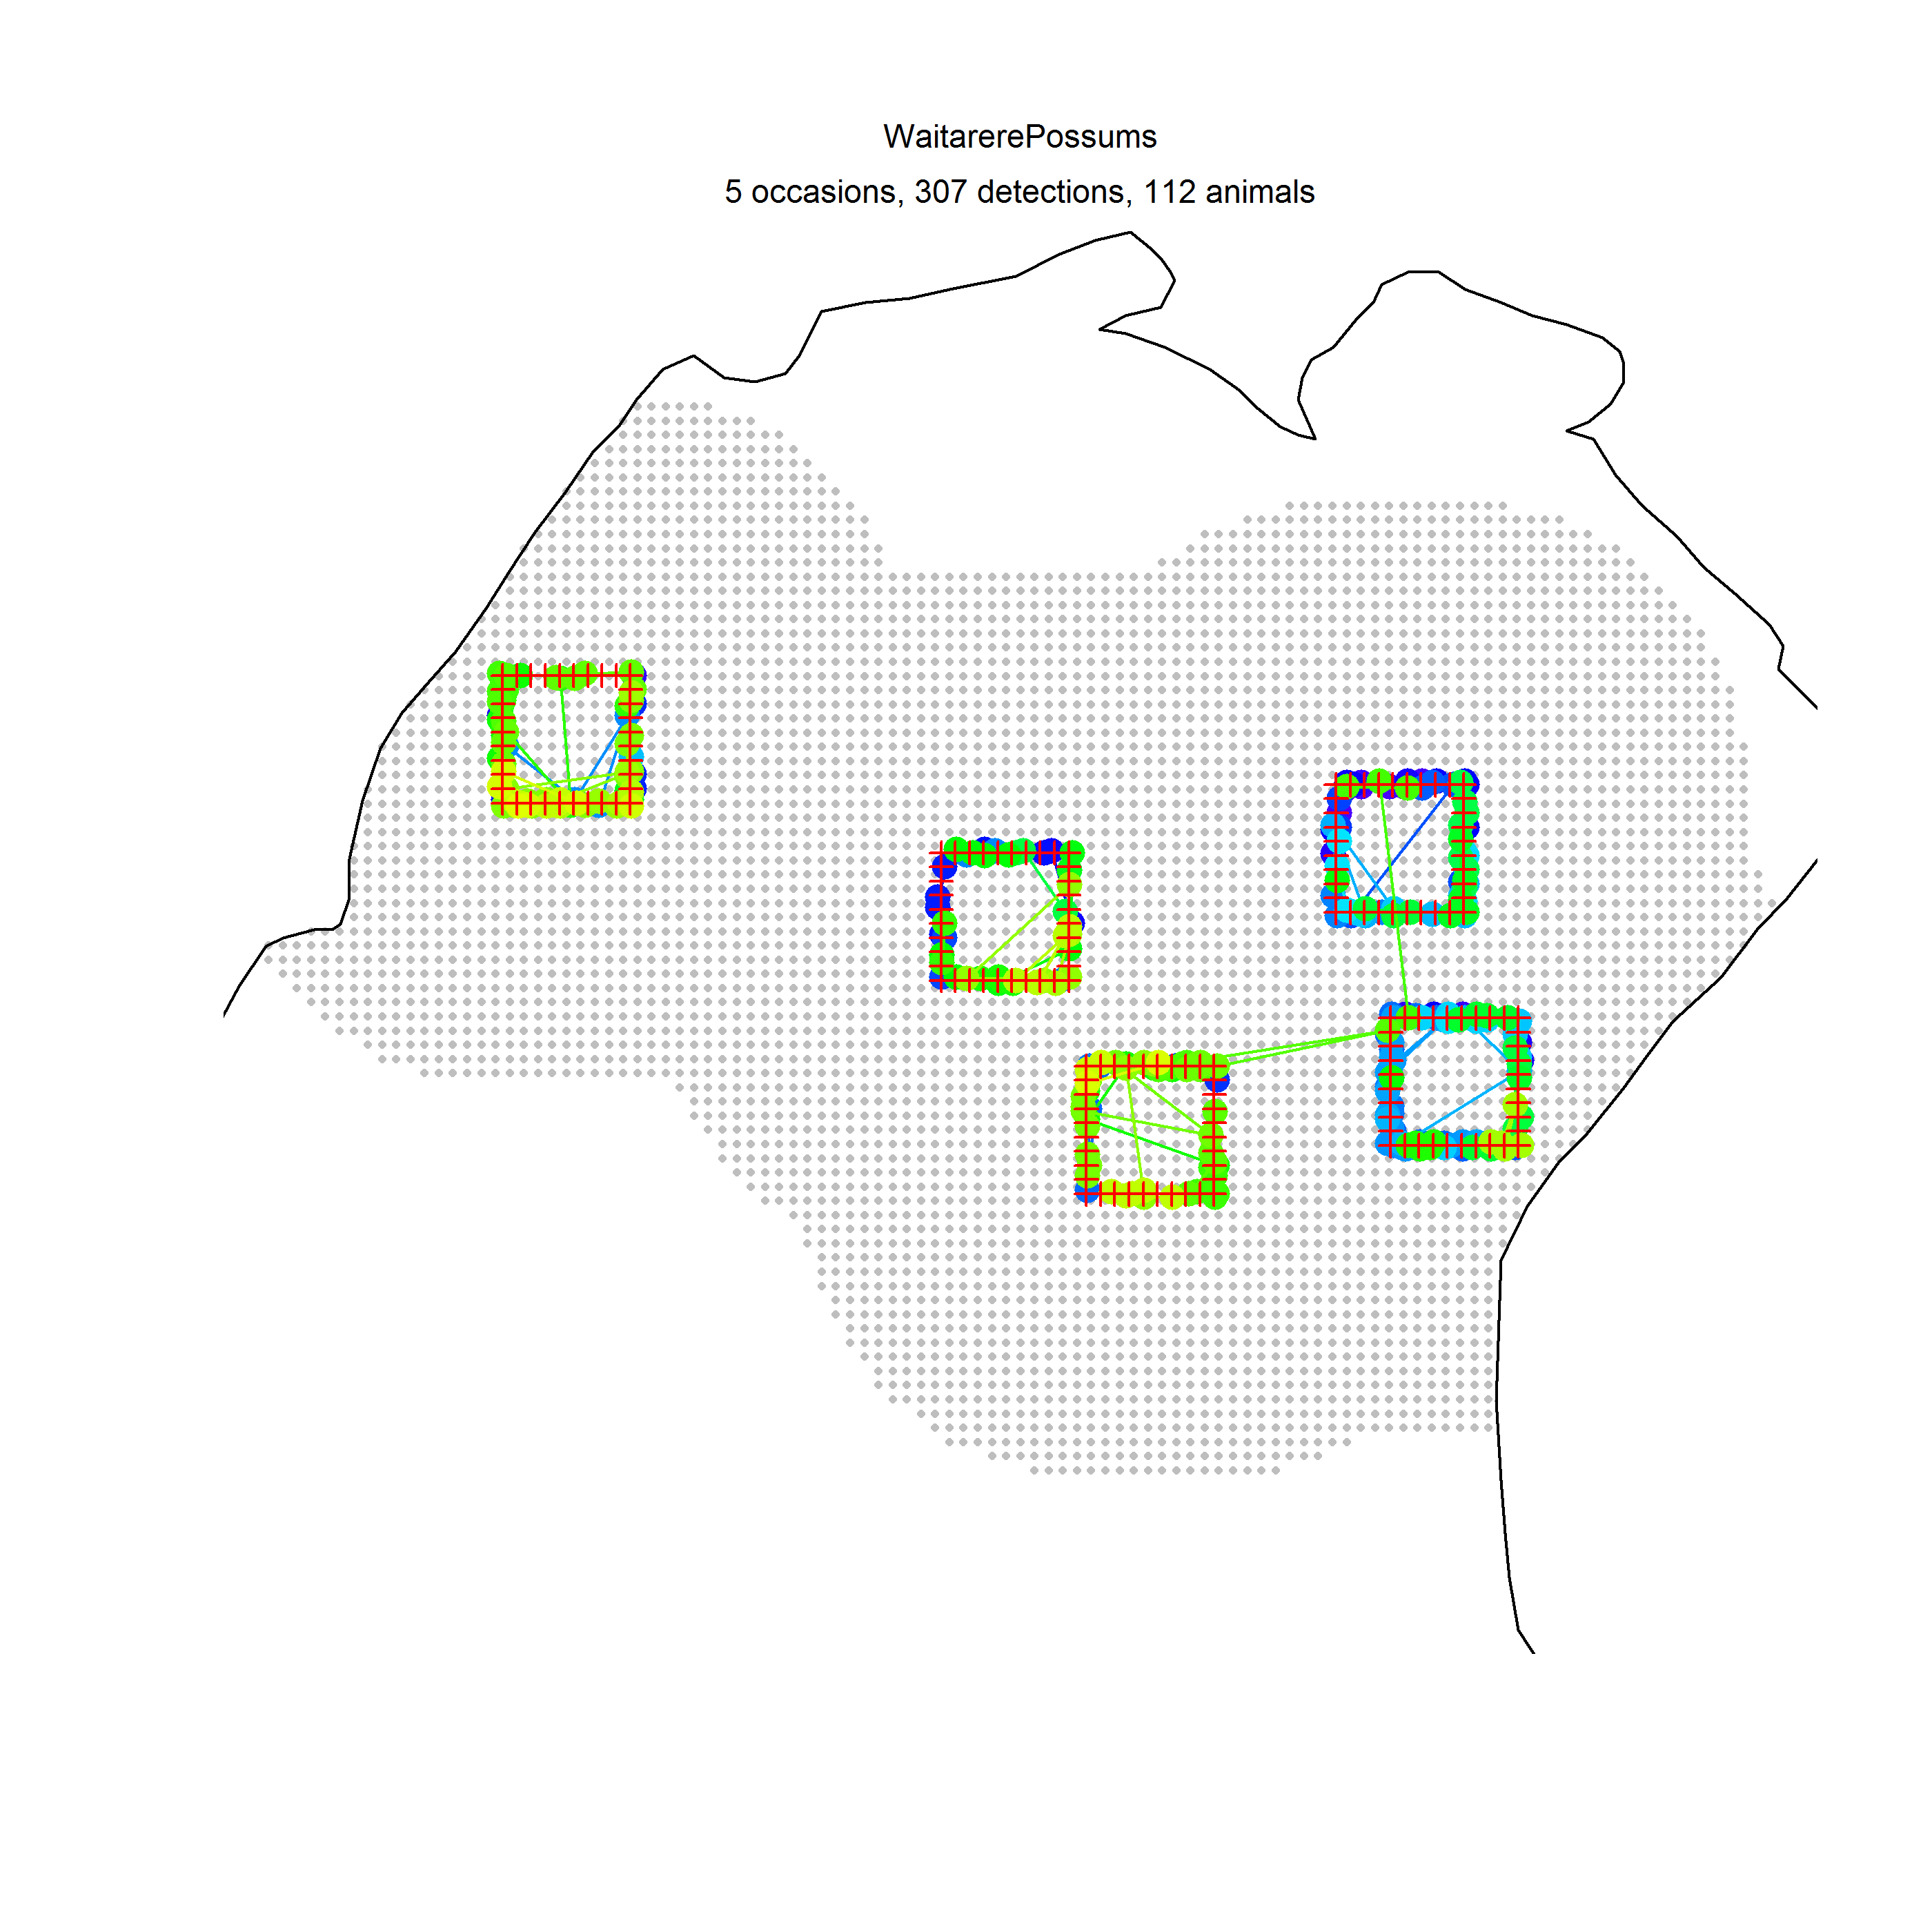
\includegraphics[width=5in,height=3.2in]{Ch5-PoisMn/figs/possum.png}
\caption{Trapping grids used in possum study from
  \citet{efford_etal:2005}, data are contained in the \R
package \mbox{\tt secr}
\citep{efford:2011}, refer to the help file \mbox{\tt ?possum} for
additional details of this study.}
\label{poisson-mn.fig.possum}
\end{figure}

The data file \mbox{\tt possumCH} contains 112 encounter histories,
and we analyzet those here although the last 8 of those are recaptures
treated as new individuals\footnote{M. Efford, personal communication}.
%Trapping produced
%46 adult females, 33 adult males, 10 immature females and 11
%immature males; sex and/or age were not recorded for 4 individuals
%(M. Coleman unpubl. data).
The encounter process is not strictly a single-catch multinomial process because,
as noted in the \mbox{\tt possum} help file
 ``One female possum was twice captured at two
sites on one day, having entered a second trap after being released;
one record in each pair was selected arbitrarily and discarded.''
which is a similar problem as we might have in bird mist net studies.
If this was a significant problem then it might be worth describing a
model fo $n_{ik} = $ the number of captures of individual $i$ during
sample $k$ to make use of all captures. By discarding the two
extra-capture events, we can satisfactorily view these data as
single-catch data, for which \mbox{\tt secr} uses the independent
multinomial likelihood (M. Efford, pers. comm.).

For our analysis we just tossed up a rectangular state-space which
doesn't account for any geographic boundaries of the suvey region, but
we note that a habitat mask is included in \secr, and we analyze the
data using that mask in Chapt. \ref{chapt.mle}.
Whether or not we use the mask is
probably immaterial as long as we understand the predictions of $N$ or
$D$ over the ocean don't mean anything biological and we probably
wouldn't report such predictions.

XXX add code here
to set up the analysis we do this.....
XXXXX

XXXX Script for doing this needs to be put in the repo XXXXXXX
Note that we define Dha in the WinBUGS script.
XXX This is fashioned after the ind. multinomial model.

{\small
\begin{verbatim}
> summary(out2)

Iterations = 501:2500
Thinning interval = 1
Number of chains = 3
Sample size per chain = 2000

1. Empirical mean and standard deviation for each variable,
   plus standard error of the mean:

             Mean        SD  Naive SE Time-series SE
D       1.541e-04 1.223e-05 1.579e-07      6.113e-07
Dha     1.541e+00 1.223e-01 1.579e-03      6.113e-03
N       2.342e+02 1.858e+01 2.399e-01      9.288e-01
alpha0 -7.380e-01 1.539e-01 1.987e-03      6.189e-03
alpha1  1.952e-04 2.052e-05 2.649e-07      1.302e-06
psi     4.686e-01 4.282e-02 5.528e-04      2.002e-03
sigma   5.082e+01 2.691e+00 3.474e-02      1.711e-01

2. Quantiles for each variable:

             2.5%        25%        50%        75%      97.5%
D       1.316e-04  1.455e-04  1.534e-04  1.619e-04  1.797e-04
Dha     1.316e+00  1.455e+00  1.534e+00  1.619e+00  1.797e+00
N       2.000e+02  2.210e+02  2.330e+02  2.460e+02  2.730e+02
alpha0 -1.043e+00 -8.411e-01 -7.387e-01 -6.368e-01 -4.308e-01
alpha1  1.565e-04  1.811e-04  1.949e-04  2.086e-04  2.379e-04
psi     3.876e-01  4.400e-01  4.675e-01  4.957e-01  5.563e-01
sigma   4.584e+01  4.896e+01  5.065e+01  5.254e+01  5.652e+01
\end{verbatim}
}

The estimated density (posterior mean) is about 1.54 possums/ha which
compares well with the estimated obtained from \secr (see
Chapt. \ref{chapt.mle} for more on the use of \secr).
To fit these data we do this (default to half-normal function)
\begin{verbatim}
secr.fit( capthist = possumCH, trace = F )
\end{verbatim}
which produces summary output like this
\begin{verbatim}
[... some output deleted ...]

Fitted (real) parameters evaluated at base levels of covariates
       link   estimate SE.estimate        lcl        ucl
D       log  1.6988930  0.17352645  1.3913904  2.0743547
g0    logit  0.1968542  0.02256272  0.1563319  0.2448321
sigma   log 51.4689114  2.59981905 46.6204139 56.8216500

[... some output deleted ...]
\end{verbatim}
There are a million reasons for potential differences some of which
we've discussed in the context of Bayesian and likelihood estimates
(Chapt. \ref{chapt.closed} sec. XXXX).
But even among likelihood estimates -- any time you run a model there
is some numerical integration going on which requires some specific
choices of how to do the integration (see
Chapt. \ref{chapt.mle}). Also \secr uses the conditional likelihood
\citep{borchers_efford:2008} which we expect to induce a slight
difference.
For now we just observe that the estimated density is certainly in the
ballpark and so too is the estimated $\sigma$.






\section{Summary and Outlook}

In this chapter we extended the basic SCR model structure to
accommodate alternative observation models, including Poisson and
multinomial observation models.
Along with the binomial model described in Chapt. \ref{chapt.scr0},
this sequence of models will accommodate the vast majority of
contemporary spatial capture-recapture problems. These models provide
the general framework for modeling the 3 main types of encounter data:
binary encounters, multinomial trials from ``multi-catch'' or
``single-catch'' \citep{efford:2004, efford:2011} trap systems, and encounter frequency
data from devices that can record multiple encounters of the same
individual at a device.

The single-catch system, as a sequence of dependent multinomial trials
(essentially a removal process operating on traps) we only did a ad
hoc analysis of this.
Figuring out the formal analysis of the single catch system would be
a nice research project for a grad student or something.
Seems like order of capture needs to be integrated into the model somehow.

There are other types of encounter models that arise in
practice. We identify a few of them here, although we neglect a
detailed development of them at the present time or, in some cases, put that off until
later chapters.
(1) Removal systems. Sometimes traps kill individuals and SCR models can handle
that. This can be viewed as a kind of open model, with mortality only, and we handle that
in Section XXXX Beth? XXXX;
(2) Trapping webs: REF XXX XXXX
would be possible to formulate trapping webs as a hierarchical model
but we haven't pursued this because trapping webs are simply not used
in practice, or their use is extremely rare.  Idea is that competition
among traps .... dividing constant density of individuals into a
variable density of traps...;
(3) Acoustic devices; What is this thing? XXXXX We need a 2 sentence
summary here... XXXX;
(4)
There are models for which
only specific summary statistics are observable
\citep{chandler_royle:2012}
which we cover in Chapts. \ref{chapt.scr-unmarked}-
\ref{chapt.partialID};
(5) We can have multiple observation methods working together as in
\citet{gopalaswamy_etal:2012} which we summarize in sec. XXXXX;
(6) In so-called search-encounter models we have slightly different
considerations -- there is an intermediate ``process'' related to
movement and so our observations.... not sure how to discuss that here.








\chapter{
Modeling Space Usage:
Integrating Resource Selection Information with
Spatial Capture-Recapture
  Models}

\markboth{Resource Selection and Space Usage}{}
\label{chapt.rsf}


\vspace{.3in}

Up to this point we have developed many variations of
SCR models to describe the observation process. 
These included models of the relationship between encounter
probability and distance, and different types of covariates such as 
behavioral responses 
that can affect detection
probability. 
Although these different observation models are immensely useful, they
are rather basic in the sense
that they imply simplistic models of how individuals use space
(section \ref{scr0.sec.implied}) and how individuals are distributed
in space.  In the following several chapters we generalize some of the
core SCR assumptions to accommodate more realistic notions of how
animals use space.

In this chapter we extend our notion of encounter probability models
as models of space usage or resource selection
(sec. \ref{scr0.sec.implied}), by extending them to include one or
more explicit landscape covariates, which the investigator believes
might affect how individual animals use space within their home range
(this is what \citep{johnson:1980} called {\it third-order} selection). We do this in a way
that is entirely consistent with the manner in which classical
``resource selection function'' (RSF) models \citep{manly_etal:2002} or utilization
distributions \citep{worton:1989, fieberg:2005, fieberg:2007}are estimated from animal
telemetry data.  In fact, we argue there that SCR models and RSF/UD
models estimated from telemetry are based on the same basic underlying model
of space usage. The important distinction between SCR and RSF studies are
that, in SCR studies, encounter of individuals is imperfect (i.e.,
``$p<1$'') whereas, with RSF data obtained by telemetry, encounter is
perfect\footnote{this is not strictly true -- rather, detection is not
  a {\it stochastic} outcome.}. We can think of the two as being
exactly equivalent either if we have a dense array of trapping
devices, or if our telemetry apparatus is imperfect such as only
samples a small area of space (this would be consistent with telemetry
stations for sampling fish which only measure passage).  A key concept
that we must confront in order to unify and integrate SCR and RSF data
is that we need to formulate both models in terms of a common latent
variable so that we can make them consistent with respect to some
underlying space utilization process. As we will explain, this latent
variable is the number of times that an individual uses a 
particular pixel of the landscape.

Here we show how to integrate standard RSF type data obtained from
telemetry into SCR models to model space usage explicitly.  This
produces asymmetric, irregular and non-stationary home ranges, and
allows us to make formal inferences about factors that influence home
range geometry and morphology directly from SCR data.  We begin by
describing a model for space usage that exists independent of how we
obtain the data (whether by telemetry or by capture-recapture). The
model posits that individuals use space in proportion to one or more
measurable covariates, say $z({\bf x})$, defined for every pixel or
location ${\bf x}$.  Then we introduce observation models consistent
with both standard capture-recapture methods and telemetry.  This
allows us to define a general likelihood function that is the product
of the two components, if they are both simultaneously available.  In
the absence of RSF data from telemetry, the model reduces to an
ordinary SCR model but with a spatial covariate $z({\bf x})$ affecting
encounter probability.

Following \citet{borchers_efford:2008}, we provide a formal
likelihood-based analysis of the model, and carry-out a simulation
study for various sample sizes of telemetered individuals to evaluate
the improvement from adding telmetry information to SCR studies and
{\it vice versa}.
The modeling framework we develop here simultaneously resolves
 three important
technical problems: (1) it generalizes all existing
encounter probability models for SCR data to accommodate realistic
patterns of space usage that are {\it not} symmetric and spatially
constant;
(2) It allows us to estimate RSF
parameters directly from SCR data, i.e., {\it absent} telemetry data;
and (3) it allows us to integrate telemetry data directly into SCR
models to improve estimates of model parameters, including density.
Our model greatly expands the applied relevance of SCR methods for
conservation and management, and for addressing applied and theoretical
questions related to animal space usage.


\begin{comment}
In our formulation we estimate the latent ${\bf s}$ variables from the observed telemetry
data, just as a convenience, but this wouldn't be necessary.
Also we assume the data are independent pieces but if some of the SCR
individuals are the same as the telemetered individuals then we should
probably account for that explicitly. So right now we pretend we don't
know anything about the telemetered guys in terms of their capture
history. So they don't contribute to information about baseline
encounter probability, just to estimates of the other encounter model
parameters.
\end{comment}



\section{Basic Model of Space Usage}
\label{rsf.sec.rsfmodel}

We develop the model here in terms of a discrete landscape purely for
computational expediency. That said, essentially no landscape on your
computer is continuous, except in the rare case that the landscape is
defined strictly in terms of variables that themselves are inherently
continuous -- e.g., ``distance to road'' or something like that.  But
almost all habitat or landscape structure data comes to us in the form
of raster data.  Let ${\bf x}_{1},\ldots,{\bf x}_{nG}$ identify the center
coordinates of a set of $nG$ pixels that define a landscape.
We organize them into a matrix
${\bf X}_{nG \times 2}$.  Let $z({\bf x})$ denote a covariate measured
(or defined) for
every pixel ${\bf x}$. For clarity, we develop the basic ideas here in terms of a
single covariate but, in practice, investigators typically have more
than 1 covariate. The formulation of the model is unaffected by
whether we have one or multiple such covariates.

We suppose that a population of individuals wanders around space in
some manner related to the covariate $z({\bf x})$, and their locations
accumulate in pixels by some omnipotent accounting mechanism. We will
define ``use of ${\bf x}$'' to be the event that an individual animal
appeared in some pixel ${\bf x}$. This is equivalently stated in the
literature in terms of individual having {\it selected} ${\bf x}$ but
the latter term implies some kind of 
conscious intent, and so we keep to the term {\it use} as much as
possible.
As a biological matter, use is the outcome of
individuals moving around their home range but, i.e., where an
individual is at any point in time is the result of some movement
process. But, to understand space usage, it is not necessary to
entertain explicit models of movement, just to observe the outcomes,
and so we don't elaborate further on what could be sensible or useful
models of movement.

Let $n_{ij}$ be the number of times individual $i$ used pixel $j$
during some period of time, i.e., the use frequencies.  We assume the
following probability mass function for the distribution of use
frequencies:
\[
{\bf n}_{i} \sim \mbox{Multinom}({\bm \pi}_{i})
\]
where
\[
 \pi_{ij} = \frac{ exp( \alpha_{2} z({\bf x}) ) }{ \sum_{x}
   exp(\alpha_{2} z({\bf x}))}
\]
This is the standard RSF model \citep{manly_etal:2002} used to model
telemetry data.  The parameter $\alpha_2$ is the effect of the
landscape covariate $z({\bf x})$ on the relative probability of
use. Thus, if $\alpha_2$ is positive, the relative probability of use
decreases as the covariate increases. In practice, we don't get to
observe $n_{ij}$ for all individuals but, instead, only for a small
subset which we capture and install telemetry devices on.  For these
telemetered individuals we accumulate individual- and pixel-specific
frequencies, at a lower sampling rate than actual individual use. For
example, we might choose to record the location of an individual every
hour or day or whatever. As such, the observed frequency of pixel use
is a {\it sample} of use but, if the recording is random or systematic
(or otherwise unrelated to {\it where} individuals are located), then
we can imagine that the same model of space usage applies. Formally,
we suppose that the observed frequencies are a binomial sample with
sample size $n_{ij}$ and sampling intensity $\phi_{0}$ lets say, and
we see that the constant $\phi_{0}$ cancels from the expression for
the multinomial cell probabilities above. 
Therefore, for the
telemetered individuals, we adopt the standard RSF model which has
probabilities as above:
\[
 \pi_{ij} = \frac{ exp( \alpha_{2} z({\bf x}_{j}) ) }{ \sum_{x}   exp(\alpha_{2} z({\bf x}_{j}))}
\]
We extend this model slightly to make it more realistic spatially. Let
${\bf s}$ denote the centroid of an individuals home range and let
$D_{ij} = ||{\bf x}_{j} - {\bf s}_{i}||$ be the distance from the home
range center of individual $i$, ${\bf s}_{i}$, to pixel $j$, ${\bf
  x}_{j}$. We modify the space usage model to accommodate that space
use will be concentrated around an individuals home range centroid:
\begin{equation}
 \pi_{ij} = \frac{ exp( -\alpha_{1} D_{ij}^{2} +\alpha_{2} z({\bf x}_{j}) ) }
{ \sum_{x} exp(-\alpha_{1} D_{ij}^{2} +\alpha_{2} z({\bf x}_{j}))}
\label{rsf.eq.rsf}
\end{equation}
where $\alpha_1=1/(2\sigma^2)$ describes the rate at which capture probability
declines as a function of distance. Note that Eq.~\ref{rsf.eq.rsf} resembles standard encounter models
used in spatial capture-recapture but with an additional covariate
$z({\bf x})$ (and see Chapt. \ref{chapt.poisson-mn}).
In particular, under this model for space usage or resource selection,
if you have no covariates at all, or if $\alpha_{2} =
0$, then
the probabilities $\pi_{ij}$ are directly proportional to the SCR
model for encounter probability.
For example, setting $\alpha_{2} = 0$, then this implies probability
of use for pixel $j$ is:
\[
p_{ij} \propto  exp( -\alpha_{1} D_{ij}^{2})
\]
so whatever function of distance we use in our RSF implies an
equivalent model of space usage (sec. \ref{scr0.sec.implied})
when used in SCR models. Another difference between this observation model
and those that we have considered previously is that it includes a
normalizing constant $\sum_{x} exp(-\alpha_{1} D_{ij}^{2} +\alpha_{2}
z({\bf x}_{j}))$, which ensures that the use distribution is a 
proper probability density function. Thus we are able to compute
the relative probability of capture in terms of distance and space use.

As an illustration of space usage patterns under this model, we
simulated a covariate that represents 
variation in habitat
structure (Fig. \ref{rsf.fig.habitat}) such as might correspond to
habitat quality.
\begin{figure}
\centering
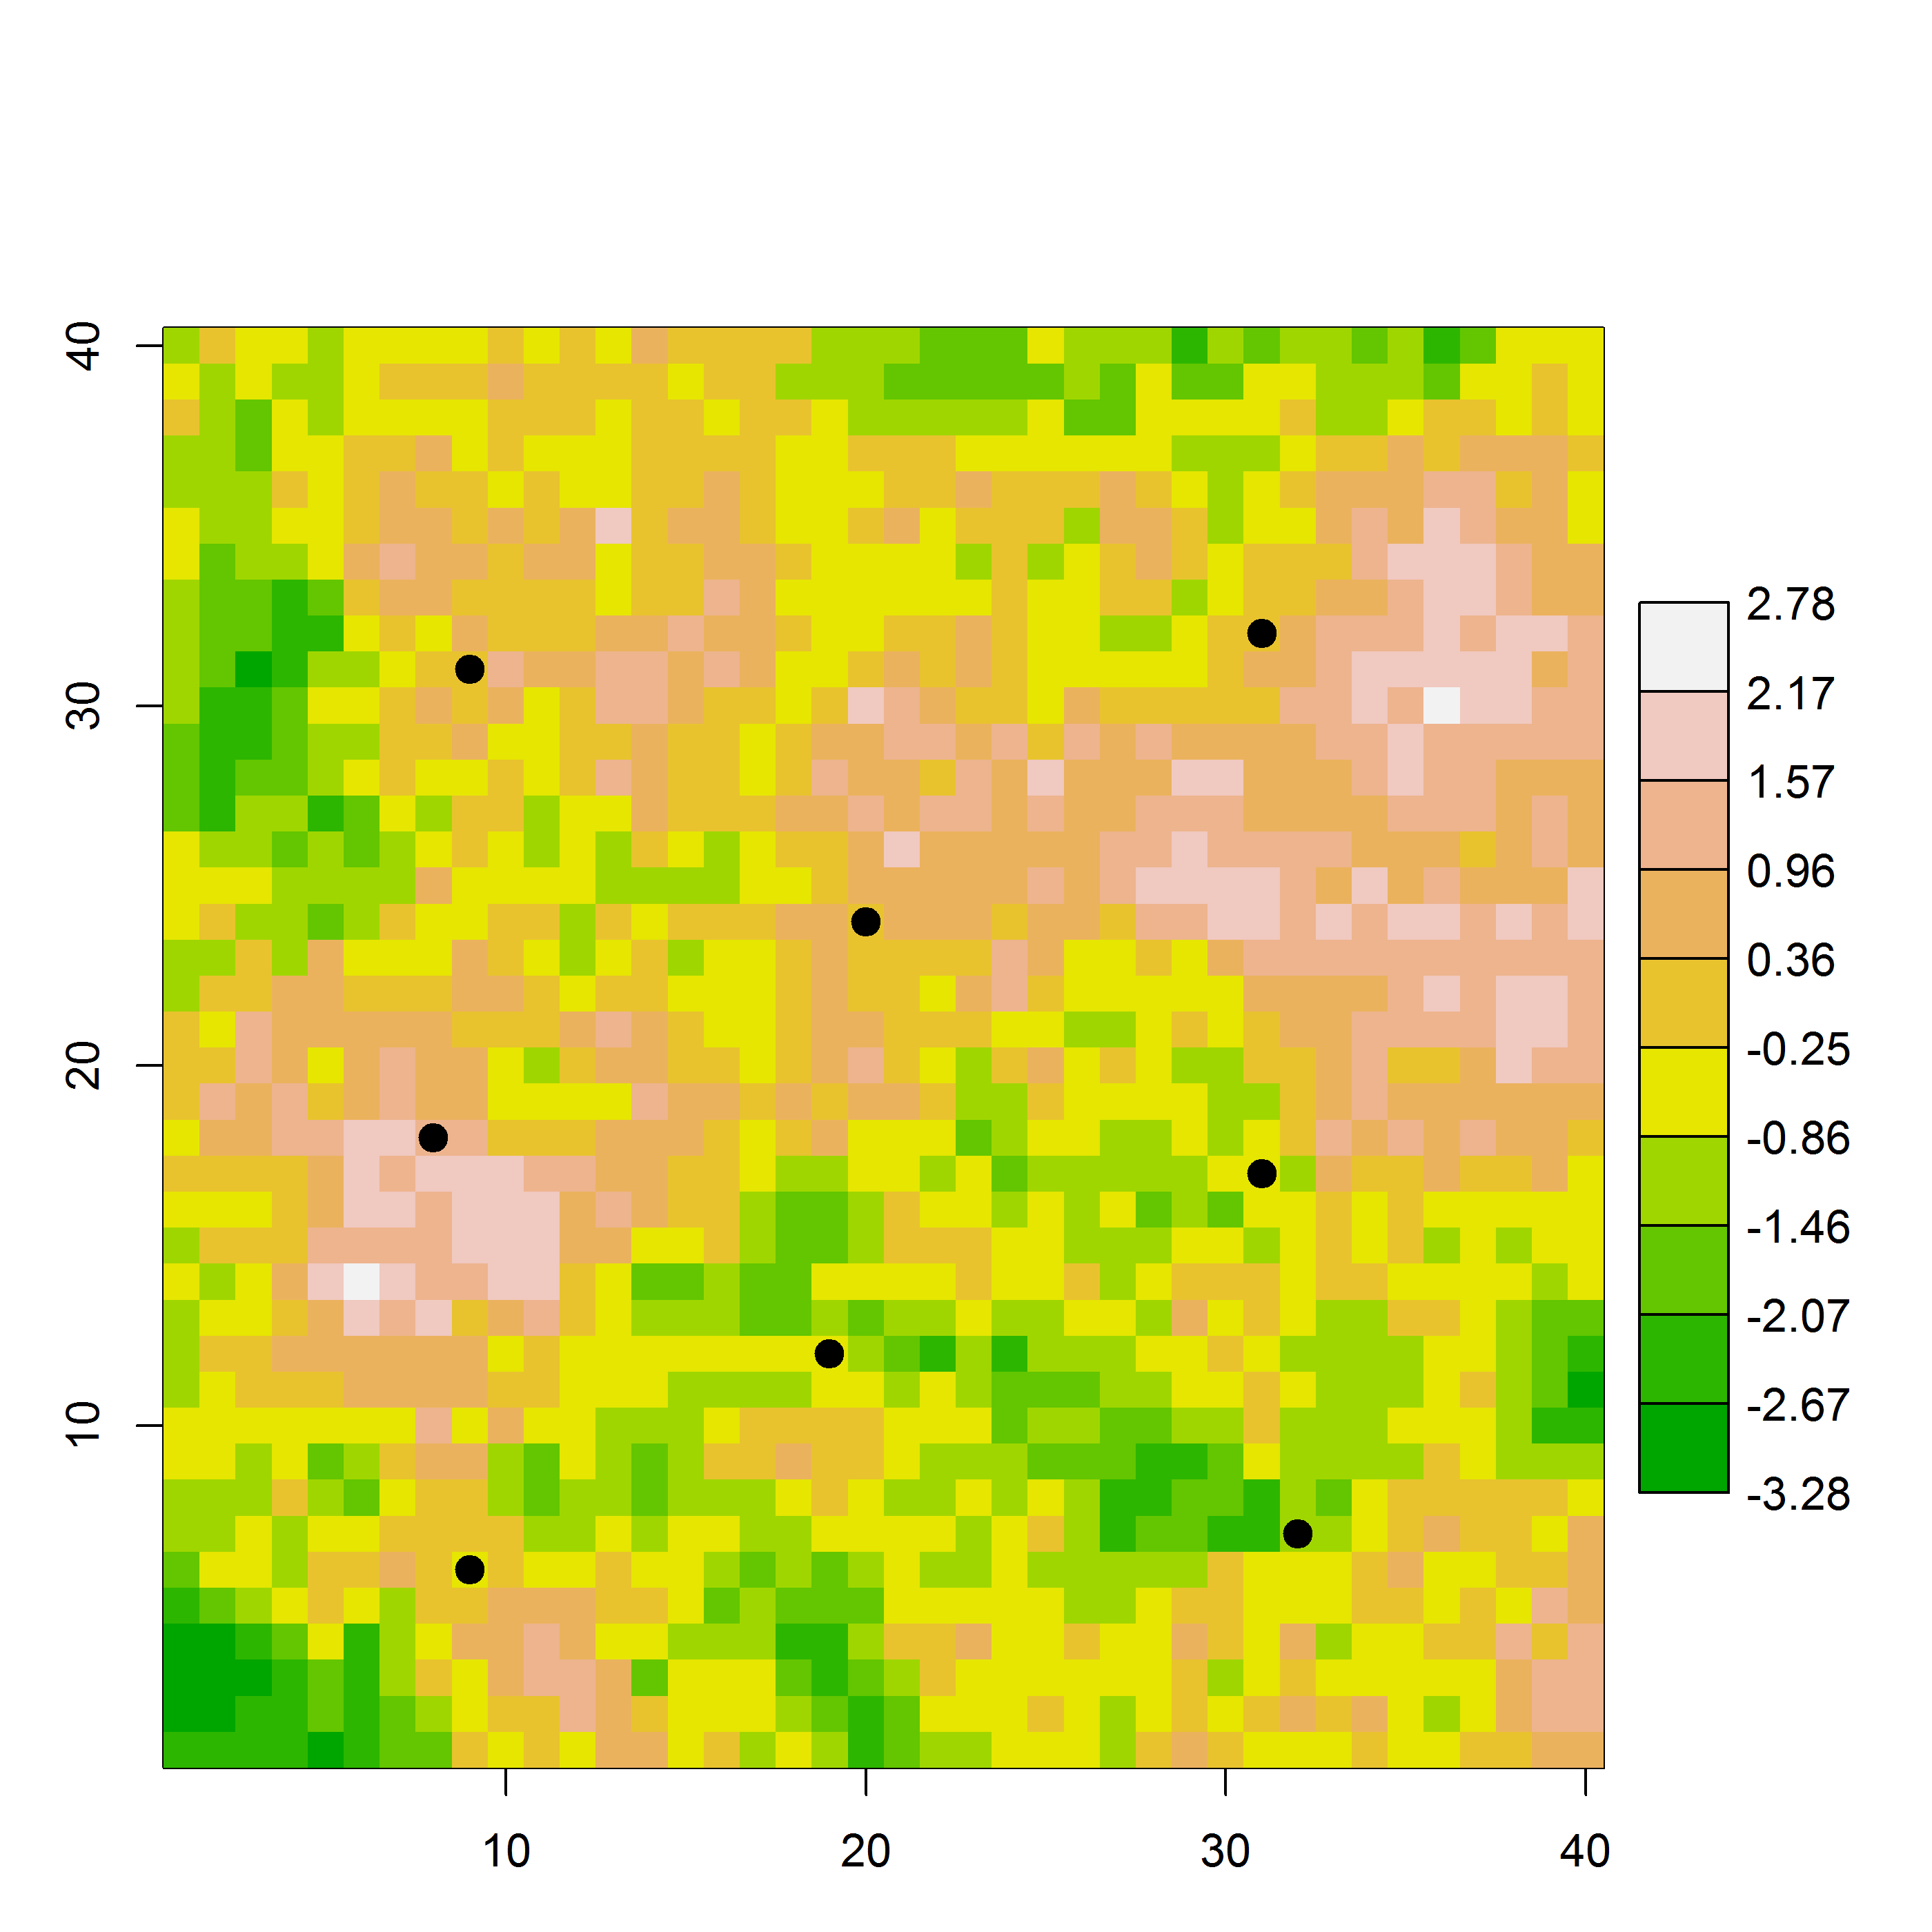
\includegraphics[width=3.5in,height=3.5in]{Ch10b/figs/habitat}
\caption{A typical habitat covariate reflecting habitat quality or
  hypothetical utility of the landscape to a species under study. Home range centers for 8 individuals are
shown with black dots.}
\label{rsf.fig.habitat}
\end{figure}
This was simulated by using a
kriging interpolator with the following {\bf R} commands:
\begin{verbatim}
set.seed(1234)
gr<-make.statespace(minx=1,maxx=40,miny=1,maxy=40,nx=40,ny=40)
Dmat<-as.matrix(dist(gr))
V<-exp(-Dmat/5)
z<-t(chol(V))%*%rnorm(1600)
spatial.plot(gr,z)
\end{verbatim}
The functions \mbox{\tt make.statespace} and \mbox{\tt spatial.plot} are
both in the \mbox{\tt scrbook} package.
Space usage patterns for
 8 individuals are shown in Fig. \ref{rsf.fig.homeranges},
simulated with $\alpha_{1} = 1/(2\sigma^2)$ with $\sigma = 2$ and the
coefficient on $z({\bf x})$ set to $\alpha_{2} = 1$.
\begin{figure}
\centering
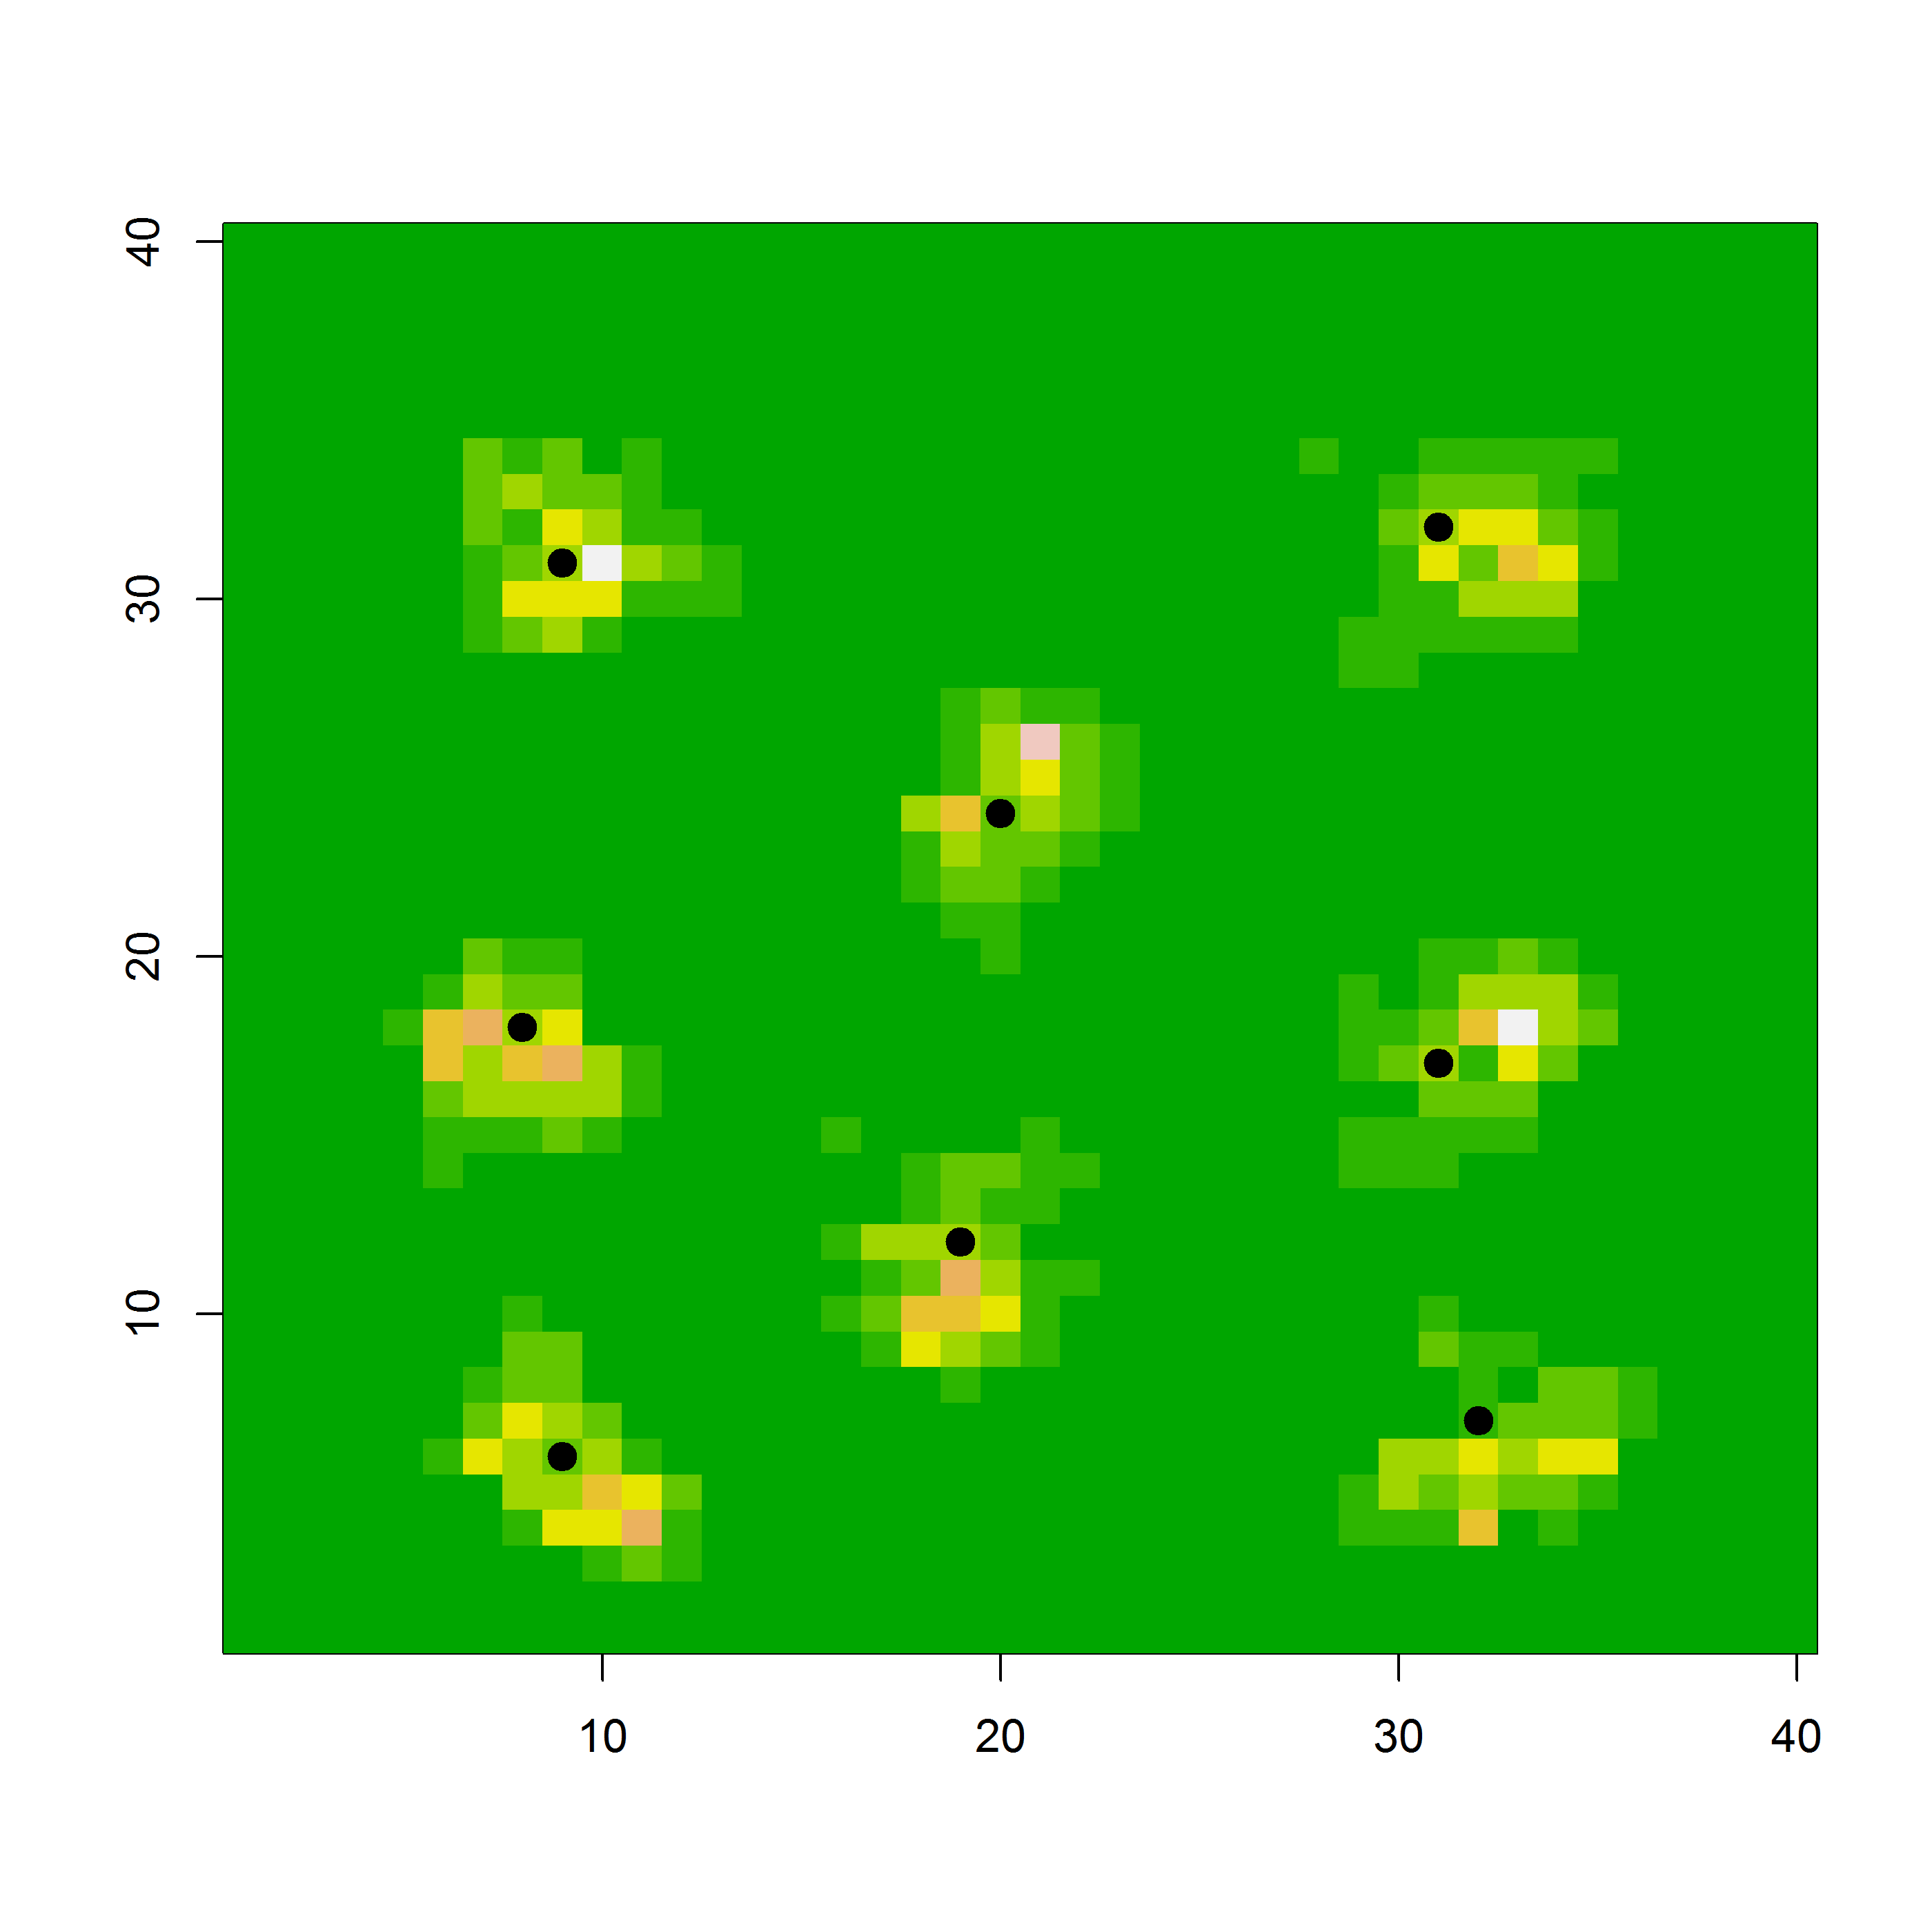
\includegraphics[width=3.5in,height=3.5in]{Ch10b/figs/homeranges8}
\caption{Space usage patterns of 8 individuals under a space usage
  model that contains a single covariate (shown in
  Fig. \ref{rsf.fig.habitat}). Plotted value is the multinomial
  probability $\pi_{ij}$ for pixel $j$ under the model in Eq. \ref{rsf.eq.rsf}.
}
\label{rsf.fig.homeranges}
\end{figure}
These space usage densities -- ``home ranges'' -- exhibit clear
non-stationarity in response to the structure of the underlying
covariate, and they are distinctly asymmetrical.  We note that if
$\alpha_{2}$ were set to 0, the 8 home ranges shown here would
resemble bivariate normal kernels with $\sigma = 2$.  Another
interesting thing to note is that the activity centers are not
typically located in the pixel of highest use or even the centroid of
usage. That is, the observed ``average'' location is not an
unbiased estimator of ${\bf s}$ under the model in
Eq. \ref{rsf.eq.rsf}. 



\subsection{Poisson use model}

A natural way to motivate this specific model of space usage is to
assume that individuals make a sequence of random resource selection
decisions so that the outcome of $n_{ij}$ are marginally {\it
  independent}, having a Poisson distribution:
\[
 n_{ij} \sim \mbox{Poisson}( \lambda_{ij})
\]
where
\[
 log(\lambda_{ij}) = a_{0} -\alpha_{1} D_{ij}^{2} +  \alpha_{2} z({\bf x})
\]
In this case,
 the number of visits to any particular cell is affected by
the covariate $z({\bf x})$ but has a baseline rate ($exp(a_{0})$) related to the amount
of movement, or number of selection decisions which is essentially
just related to the time interval over which the animal is using
space. i.e., longer time intervals lead to higher values of
$E(n_{ij})$.
This is an equivalent model to the multinomial model given previously
in the sense that, if we condition on the total sample size $n_{i.} =
\sum_{j} n_{ij}$, then the vector ${\bf n}_{i}$ has a multinomial
distribution with probabilities
\[
 \pi_{ij} = \frac{\lambda_{ij}}{ \sum_{j} \lambda_{ij}}
\]
as we discussed in Chapt. \ref{chapt.poisson-mn}.  We see that the
intensity parameter $a_{0}$ is not relevant for understanding
patterns of space usage. In particular, it cancels from the numerator
and denominator of the multinomial cell probabilities, analogous to
what happens under sampling of individual use decisions as discussed
above.

\begin{comment}
{\bf note:} while Poisson -> multinomial, it is not vice versa. If the total
sample size per individual is fixed, then the marginals are NOT
Poisson and that model will produce biased estimators.

For purposes of estimation we can use either the Poisson or
multinomial likelihoods. In the former case, we have to estimate an
individual-specific nuisance
parameter $a_{0}$, from which information is derived by the total
number of observations whereas, in the later case, we lose information
about $a_{0}$ by conditioning on the total (i.e., treating it as
fixed).  As it often is fixed, or at least the number of telemetry
observations is completely arbitrary, $a_{0}$ is usually a meaningless
parameter so whether we estimate it or not is immaterial from a
practical standpoint.
\end{comment}

\subsection{Thinning}

Suppose our sampling is imperfect so that we only observe a smaller
number of telemetry fixes than actual uses, $n_{ij}$. As developed in
sec. \ref{scr0.sec.implied}, we assume that the observed number of
uses is
\[
 m_{ij} \sim \mbox{Bin}(n_{ij}, \phi_{0}).
\]
In this case, the marginal distribution of $m_{ij}$ is also Poisson
but with mean
\[
 log(\lambda_{ij}) = log(\phi_{0}) + a_{0} -\alpha_{1} D_{ij}^{2} +  \alpha_{2} z({\bf x}).
\]
In this case, the space-usage model (RSF) for the
thinned counts $m_{ij}$ is the same as the space-usage model for the
original variables $n_{ij}$.  This is because if we remove $n_{ij}$
from the conditional
 model by summing over its possible values, then the vector of
${\bf m}_{i}$ is multinomial with cell probabilities
\[
\frac{\phi_{0}\lambda_{ij}}{\sum_{j} \phi_{0} \lambda_{ij}}
\]
and we see that $\phi_{0}$ cancels from the numerator and
denominator. XXXX not really elucidating here XXXXXXX

%That is,
%given our sequence of
%independent Poisson random variables and we condition on their total,
%i.e., regard it as fixed, then we have the multinomial. In the
%multinomial we lose information about the intercept which in this case
%is ok because we only care about the interpretation of the resource
%selection model as a probability distribution and don't care about the
%basic rate of detection -- and it is a confounding of animal use and a
%fixed sampling intensity.

In summary, if we conduct a telemetry study we observe ${\bf n}_{i}$,
the $nG \times 1$ vector of pixel-counts for each individual
$i=1,\ldots,N_{tel}$.  We declare these data to be
``resource-selection data'' which are typical of the type used to
estimate resource-selection functions (RSFs) \citep{manly_etal:2002}.
Sometimes in RSF modeling activities people make believe they have
continuous covariates and so the denominator in Eq. \ref{rsf.eq.rsf}
involves an integration over a distribution for the covariate which is
the conditional intensity of observed point locations in a point
process model. However, in a discrete landscape, entertaining pdfs for
the covariates isn't necessary \citep{royle_etal:2012mee}.\hl{Or is it
  that they ignore the fact that they are sampling 2D space? They seem
  to act as if they are sampling K-dimensional covariate space.}
\hl{yea, this could be it. lets contemplate this}

\subsection{Capture-recapture Data}

The key to combing RSF data with SCR data is to work with this
underlying resource utilization process and formulate SCR models in
terms of that process. For SCR models, the frequency of use for each pixel
serves as a intermediate
latent that we don't get to observe. We assume that, fundamentally,
both telemetered individuals and SCR individuals are using space
according to the same resource selection model. The difference is that,
for SCR data, we 
do not have sampling devices in all locations (pixels) in the landscape, and hence the
data are only recorded at a subsample of them.
In other words, imagine that we have a sampling device, such as a
camera trap, in {\it every} pixel. If the device operates continually
then it is no different from a telemetry instrument. If it
operates  intermittently and does not expose the entire area of
each pixel then a reasonable model for this imperfect observation is
the ``thinned'' binomial model given above, where $\lambda_{0}$
represents the sampling effectiveness of the device. So we imagine
that the hypothetical perfect data from a camera trapping study are
the counts $m_{ij}$.

We then construct our SCR encounter probability model based on the
view that these frequencies $m_{ij}$ are {\it latent}. In particular,
under the SCR model with binary observations,
 we observe a random variable
$y_{ij} = 1$  if the individual $i$ visited the pixel
containing a trap and was detected.
We imagine that $y_{ij}$ is related to the latent variable $m_{ij}$ being the
event $m_{ij}>0$, which occurs with probability
\[
 p_{ij} = 1-exp(- \lambda_{ij})
\]
where 
\[
 log(\lambda_{ij}) = log(\phi_{0}) + a_{0} -\alpha_{1} D_{ij}^{2} +  \alpha_{2} z({\bf x}).
\]
and we collect the constants so that $\alpha_{0} = log(\phi_{0}) +
a_{0}$ is the 
 baseline encounter rate which includes
the constant intensity of use by the individual and also the baseline
rate of detection, conditional on use.



\section{The Joint RSF/SCR Likelihood}

To construct the likelihood for SCR data when we have auxiliary
covariates on space usage {\it or} direct information on space usage
from telemetry data, we regard the two samples (SCR and RSF) as
independent of one another. In practice, this might not always be the
case but (1) often time the telemetry data come from a previous study;
(2) the individuals are not the same at all; (3) or even if they are
some of the same individuals being captured, we might not be able to
match individuals captured by a sampling method such as hair-snares
with the individuals wearing radio-collars; (4) In cases where we {\it
  can} match some individuals between the two samples, regarding them as
independent should only entail a minor
loss of efficiency
because we are disregarding more precise information on a small number
of activity centers. Moreover, we believe, it is unlikely in practice
to expect the two samples to be completely reconcilable and that the
independence formulation is the most generally realistic.

Regarding the two data sets as being independent, our approach here
is to form the likelihood for each set of observations as a function
of the same underlying parameters and then combine them. In
particular, let ${\cal L}_{scr}(\alpha_{0}, \alpha_{1}, \alpha_{2}, N;
{\bf y}_{scr})$
be the likelihood for the SCR data in terms of the basic encounter
probability parameters and the total (unknown) population size $N$,
and let ${\cal L}_{rsf}(\alpha_{1},\alpha_{2}; {\bf m}_{rsf})$ be the
likelihood for the RSF data based on telemetry which, because the
sample size of such individuals is fixed, does not depend on $N$.
The
joint likelihood is the product of these two pieces:
\[
{\cal L}_{rsf+scr}(\alpha_{0},\alpha_{1},\alpha_{2},N; {\bf y}_{scr},{\bf
  m}_{rsf})  = {\cal L}_{scr} \times {\cal L}_{rsf}
\]
In what follows, we provide a formulation of each likelihood
component, along with an {\bf R} function for obtaining the MLEs of
model parameters using standard methods available in {\bf R}.

The observation model for the SCR data for individual $i$ and trap $j$,
from sampling over $K$ encounter periods, is:
\[
 y_{ij}|{\bf s}_{i} \sim \mbox{Bin}(K; p_{ij})
\]
where
\[
 p_{ij} = 1-exp(- \lambda_{ij} )
\]
and
\[
 \lambda_{ij} = \lambda_{0} exp(- \alpha_{1} D_{ij}^{2} + \alpha_{2}  z(x_{j}) )
\]
A compact expression of these model components is:
\begin{equation}
y_{ij}| {\bf s}_{i} \sim \mbox{Bin}(K, p_{\alpha}(D_{ij}; {\bm \alpha}))
\label{rsf.mle.eq.cond-on-s}
\end{equation}
We emphasize that this is conditional on the latent variables ${\bf
  s}_{i}$ (which appear in $D_{ij}$). For these latent variables we
adopt the standard assumption of uniformity, ${\bf s}_{i} \sim
\mbox{Unif}({\cal S})$.  The joint distribution of the data for
individual $i$, conditional on ${\bf s}_{i}$, is the product of $J$
binomial terms (i.e., the contributions from each of $J$ traps):
\[
  [{\bf y}_{i} | {\bf s}_{i} , {\bm \alpha}] =
  \prod_{j=1}^{J} \mbox{Bin}(K, p_{\alpha}({\bf x}_{j},{\bf s}_{i}) )
\]
The so-called marginal likelihood \citep{borchers_efford:2008} is
computed by removing ${\bf s}_{i}$, by integration, from the
conditional-on-${\bf s}$ likelihood and regarding the {\it marginal}
distribution of the data as the likelihood. That is, we compute:
\[
  [{\bf y}_{i}|{\bm \alpha}] =
\int_{{\cal S}}  [ {\bf y}_{i} |{\bf s}_{i},{\bm \alpha}] g({\bf s}_{i}) d{\bf s}_{i}
\]
{\flushleft where}, under the uniformity assumption, we have
$g({\bf s}) = 1/||{\cal S}||$.
The joint likelihood for all $N$ individuals,
is the product of $N$ such terms:
\[
{\cal L}_{scr}({\bm \alpha} | {\bf y}_{1},{\bf y}_{2},\ldots, {\bf y}_{N}) = \prod_{i=1}^{N}
[{\bf y}_{i}|{\bm \alpha}]
\]
Now, in practice, we don't know $N$ and so we can't just compute the
SCR likelihood in this manner. Following our development in
Chapt. \ref{chapt.mle},
we can compute the contributions of the
$n$ observed individuals, but then we have to compute the likelihood
contribution for the ``all 0'' encounter history, i.e., that
corresponding to unobserved individuals. The mechanics of computing
that are the same as for an ordinary observed encounter history. We
then have to deal with the issue that $n$ itself is a random variable,
and that leads to the combinatorial term in front of the likelihood
which involves the total population size $N$.

For the RSF data from the sample of individuals with telemetry devices
we adopt the same basic strategy of describing the
conditional-on-${\bf s}$ likelihood and then computing the marginal
likelihood by averaging over possible values of ${\bf s}$.
We have ${\bf m}_{i}$, the vector of pixel counts for individual $i$,
where these counts are derived from a telemetry study or similar.
Their likelihood contribution is
proportional to
\[
 {\cal L}_{rsf}({\bm \alpha}, {\bf m}_{rsf})
 = \prod_{g=1}^{G}  \pi_{ij} ^{m_{ij}}
\]
where
\[
 \pi_{ij} =  = \frac{ exp( -\alpha_{1} D_{ij}^{2} -\alpha_{2} z({\bf x}_{j}) ) }
{ \sum_{g} exp(-\alpha_{1} D_{ij}^{2} -\alpha_{2} z({\bf x}_{j}))}
\]

Technical details for computing the likelihood and obtaining the MLEs
are given in Appendix 1 where we provide an ${\bf R}$ function to
evaluate the likelihood and obtain the MLEs.
\begin{comment}
\begin{verbatim}

Script here

\end{verbatim}
\end{comment}
A key practical detail
is that the likelihood here is formulated in terms of the parameter
$N$, the population size for the landscape defined by ${\cal
  S}$. Given ${\cal S}$, density is computed as $D({\cal S}) =
N/||{\cal S}||$. In our simulation study below we report $N$ as the
two are equivalent summaries of the data set once ${\cal S}$ is
defined.


\section{Illustration}


We carried-out a simulation study using the landscape shown in
Fig. \ref{rsf.fig.habitat}, and based on a population of $N=100$
individuals with activity centers distributed uniformly over the
landscape.  This patchy covariate was simulated by generating a field
of spatially correlated noise to emulate a typical patchy habitat
covariate such as tree or understory density, or some other covariate
relevant to habitat quality for a species.  We subjected individuals
to sampling over $K=10$ sampling periods, using a $7 \times 7$ array
of trapping devices located on the the integer coordinates $(u*5,v*5)$
for $u,v = 1,2,3,4,5,6,7$. The model parameters were
\[
 cloglog(p_{ij}) = -2 -xyz -xyz....
\]
and these settings yielded an average of $n=61$ individuals captured.
In addition to simulating data from this capture-recapture study, we
simulated 2, 4, 8, 12, 16 telemetered individuals to assess the
improvement in precision as sample size increases.  For all cases we
observed 20 telemetry fixes {\it per} individual.  The main things
we're focused on with this simulation study were: (1) how much does
the SE of estimated $N$ improve as we add or increase the number of
telemetered individuals?  (2) How well does the SCR model do at
estimating the parameter of the RSF with {\it no} telemetry data?  (3)
How much does the precision of the RSF parameter improve if we add SCR
data to the telemetry data?


%% Should also simulate fitting the wrong model with symmetric
%% encounter model and see what happens
%% also run N=200 with 500 iterations

\begin{verbatim}
300 iters each
n=2           Nhat RMSE  ahat RMSE  sighat  RMSE
SCR only:   99.73  9.97  0.99  0.14  2.00  0.124
SCR/RSF:    99.94  9.54  0.99  0.12  2.00  0.097
sbar        98.89  9.50  0.93  0.14  1.97  0.100
RSF only     --    --    1.03  0.33  2.00  0.160
n=4
SCR only    99.10  9.83  0.99  0.13  2.00  0.127
SCR/RSF     99.17  9.47  0.99  0.11  2.00  0.086
sbar        97.43  9.68  0.89  0.16  1.97  0.090
RSF only     --     --   0.98  0.22  2.00  0.119
n=8
SCR only    99.59 10.00  1.00  0.13  2.00  0.130
SCR/RSF     98.90 10.02  0.99  0.10  2.00  0.071
sbar        96.07 10.37  0.84  0.19  1.96  0.078
RSF only     --    --    0.98  0.16  2.01  0.084
n=12
SCR only    99.44 10.73  0.98  0.13  2.02  0.128
SCR/RSF     99.96 10.26  1.00  0.09  2.00  0.059
sbar        96.30 10.49  0.82  0.20  1.96  0.071
RSF only     --    --    1.01  0.12  2.00  0.069
n=16
SCR only    99.23 10.74  0.99  0.14  2.00  0.128
SCR/RSF     99.20  9.79  1.00  0.09  1.99  0.057
sbar        95.10 10.17  0.80  0.22  1.95  0.075
RSF only     --    --    1.00  0.10  1.99  0.061
\end{verbatim}

The replicate runs of the SCR-only situation give us an idea of the
inherent MC error in these simulations, which is roughly about
0.25. This result suggests there is a small persistent bias of $< 1\%$
in the MLE of $N$ in general, and as much as 2-4\% when ${\bf s}$ is
estimated by the average observed location.  In general we expect a
small amount of bias in MLEs as likelihood theory only guarantees
asymptotic unbiasedness and, here, we only have 61 individuals being
captured, on average.  Moreover, the raster is fairly coarse relative
to $\sigma$ in our study, having a 1 km resolution whereas $\sigma =
2$, which we expect to introduce a small amount of negative bias
because it is an explicit under-statement of the true heterogeneity in
$p$ due to the spatial context of the problem.  The apparent bias that
arises as a result of esetimating ${\bf s}$ is expected because the
average location of an individual would be unbiased for ${\bf s}$ only
if the individual is moving according to a stationary isotropic
kernel. Under the model of space usage with covariate $z({\bf x})$,
then the average location is biased to favor good values of $z({\bf
  x})$ and so $\bar{\bf s}$ is really biased for ${\bf s}$. \hl{again,
  is there an unbiased estimator available?}

In terms of total precision, generally there is about a 5\% reduction
in RMSE when we have at least 2 telemtered individuals, and, although
there is a lot of MC error in the RMSE quantities, it might be as much
as a 10\% reduction (tops) as $n$ increases. This makes sense because
we nail down the parameters and still don't know where guys are, and
get info about mean p, $\alpha_{0}$ only from the SCR data. Thus
estimating $N$ only benefits slightly from the addition of telemetry
data.  \hl{I don't understand how this could be true. It seems like
  there should be a tight relationship between the uncertainty about
  $sigma$ and that of $N$?? That is what we found when we used the
  informative prior in our AOAS paper.} The key benefit of our model, therefore, is its ability to
integrate realistic patterns of space usage directly into SCR models.

Estimating the RSF parameter $\alpha_{2}$ exhibits negligible or no
bias except when ${\bf s}$ is estimated and, interestingly, it is
well-estimated from SCR data alone and even better than RSF data alone
(in terms of RMSE) until we have more than 200 or so telemetry
observations.  The big improvement comes in esetimating the home range
parameter $\sigma$ which is unbiased except when we estimate ${\bf s}$
in which case it exhibits only modest bias.  However, there is huge
improvement in RMSE of $\hat{\sigma}$, perhaps as much as 50-60\% in
some cases, but that really doesn't translate much into esetimating
$N$.



\section{Summary and Outlook}


How animals use space is a fundamental interest to ecologists, and
important in their conservation and management. Normally this is done
by telemetry and models referred to as resource selection functions
\citep{manly_etal:2002}.  Conversely, spatial capture-recapture models
have grown in popularity over the last several years
\citep{efford:2004,borchers_efford:2008, royle:2008, efford_etal:2009ecol,royle_etal:2009ecol,
  gardner_etal:2010, gardner_etal:2011, kery_etal:2010,
sollmann_etal:2011,mollet_etal:2012,gopalaswmany_etal:2012}, but
most of the development of SCR models has focused on density
estimation, not space usage.
However, it is intuitive that 
space usage should affect encounter probability and thus be highly
relevant to density estimation in SCR applications, but
this
notion of the relationship between encounter probability and space
usage has not been developed explicitly in the literature.  Indeed,
essentially all published applications of SCR models to date have been
based on simplistic encounter probability models that are symmetric,
constant among individuals and do not vary across space. One exception
is \citet{royle_etal:2012ecol} who developed SCR models that use
ecological distance metrics instead of normal Euclidean distance. Here
we developed an SCR model in terms of a basic underlying model of
space or resource use, that is consistent with existing views of
resource selection functions (RSFs) \citep{manly_etal:2002}.

In developing the SCR model in terms of an underlying model of space
usage, we achieve a number of enormously useful extensions of SCR
models. First, we have
 shown how to integrate classical RSF data from telemetry
with spatial capture-recapture data based on individual encounter
histories obtained by classical arrays of encounter devices or
traps. This leads to an improvement in our ability to estimate
density, and also an improvement in our ability to estimate parameters
of the RSF function.  Thus, the combined model is both an extension of
standard SCR models and also and extension of standard RSF models. As
many animal population studies have auxiliary telemetry information,
the ability to incorporate such information into SCR studies has
enormous applicability and immediate benefits in many studies.
Secondly, we have shown that one can estimate RSF model parameters
directly from SCR data {\it alone}. This establishes clearly that SCR
models {\it are} explicit models of space usage. Thirdly, it is also
now clear that one of the important parameters of SCR models, that
controlling ``home range radius'', is also directly estimable from
telemetry data alone. While this is of less practical relevance, it
does suggest that one might be able to estimate density with very
sparse data and few actual
recaptures of individuals, by having good estimates of $\sigma$ from
auxiliary data. This is an idea exploited by \citet{chandler_royle:2012}.

Use of telemetry data in capture-recapture studies has been suggested
previously. For example, \citet{white_shenk:2001} and
\citet{ivan:2012} have suggested using telemetry data to estimate the
vague quantity ``probability that an individual is exposed to sampling'' but
their estimator requires that individuals are sampled in proportion to
this unknown quantitiy, which seems impossible to acheive in
practice in many studies. In
addition, they do not directly integrate the telemetry data with the
capture-recapture model so that common parameters are jointly
estimated. In fact, they don't even acknowledge shared parameters of
the two models.  \citet{sollmann_etal:inprep} did recognize this, and
they used some telemetry data to estimate directly the parameter
$\sigma$ from the bivariate normal SCR model in order to improve
estimates of density. This was an important conceptual development in
the sense that it recognized the relationship between SCR models and
models of space usage, but their model did not include an explicit
resource selection component, and they did not implement a joint
estimation framework.

Our new model allows investigators to model how the landscape and
habitat influence movement and space usage of individuals around their
home range, using non-invasively collected capture-recapture data or
capture-recapture data augmented with telemetry data.  This should
improve our ability to understand, and study, aspects of space usage
and it might, ultimately, aid in addressing conservation-related
problems such as reserve or corridor design. And, it should greatly
expand the relevance and utility of spatial capture-recapture beyond
simply its use for density estimation. None of these questions
regarding space usage could be addressed using non-spatial
capture-recapture models.

We developed a formal analysis framework here based on marginal
likelihood \citep{borchers_efford:2008} (see Chapt. \ref{chapt.mle}).
In principle, Bayesian analysis does not pose any unique challenges
for this new class of models although we expect some loss of
computational efficiency due to the increased number of times the
components of the likelihood would need to be evaluated.  We imagine
that some problems would benefit from a Bayesian formulation,
however. For example, using an open population model that allows for
recruitment and survival over time \citep{gardner_etal:2010} is
convenient to develop in the {\bf BUGS} language and incorporating
information on unmarked individuals has been done using Bayesian
formulations of SCR models \citep{chandler_royle:2012,
  sollmann_etal:2012}.

In our formulation of the joint likelihood for RSF and SCR data, we
assumed the data from a capture-recapture and telemetry studies were
independent of one another. This implies that whether or not an
individual enters into one of the data sets has no effect on whether
it enters into the other data set. We cannot foresee situations in
which violation of this assumption should be problematic or invalidate
the estimator under the independence assumption.  In some cases it
might so happen that some individuals appear in {\it both} the RSF and
SCR data sets. In this case, ignoring that information should entail
only an incremental decrease in precision because a slight bit of
information about an individuals activity center is
disregarded. Heuristically, an SCR observation (encounter in a trap)
is like 1 additional telemetry observation, and so we are treating the
two pieces of information as having separate activity centers in the
model developed here.  Our model pretends that we don't know anything
about the telemetered individuals in terms of their encounter history
in traps.  In principle it shouldn't be difficult to admit a formal
reconciliation of individuals between the two lists. In that case, we
just combine the two conditional likelihoods before we integrate ${\bf
  s}$ from the conditional likelihood. This would be almost trivial to
do if {\it all} individuals were reconcilable (or none as in the case
we have covered here) but, in general , we think you will always have
an intermediate case -- i.e., either none will be or at most a subset
of telemetered guys will be known. More likely you have "well, that
guy looks telemetered but we don't know which guy it is....hmmm" and
that case, basically a type of marking uncertainty or
misclassification, is clearly more difficult to deal with.


\section*{Appendix 1: {\bf R} script for obtaining MLEs under the SCR+RSF model}
























\chapter{
%Modeling Animal space-usage with 
%Detection Models based on Ecological Distance
%Ecological Distance Models in Spatial Capture-Recapture
Modeling Space Usage: Ecological Distance in Spatial Capture-Recapture Models
}
\markboth{Chapter XXX}{}
\label{chapt.ecoldist}


\vspace{.3in}

%% this material is a general introduction for a manuscript
Spatial capture-recapture models are a relatively new class of models
for estimating animal density from capture-recapture data with
auxiliary information about individual capture locations
\citep{efford:2004,borchers_efford:2008, royle_young:2008, efford_etal:2009,
  royle_etal:2009ecol}.
The basic idea is to express encounter probability of
individuals as a function of the distance between individual center of
activity, say ${\bf s}_{i}$, and trap location, say ${\bf x}_{j}$.  
% Do we need to be clear about the i and j subscripts? ie, i=1,...,N
In these models ${\bf s}_{i}$ is regarded as a latent variable and
conventional methods of statistical inference either based on marginal
likelihood \citep{borchers_efford:2008} or Bayesian analysis by MCMC
\citep{royle_young:2008}.

While the models are a relatively recent innovation, their use is
already becoming widespread \citep{efford_etal:2009,
  gardner_etal:2010jwm, gardner_etal:2010ecol,kery_etal:2010, 
  borchers:2011,gopalaswamy_etal:2012, foster_harmsen:2012} because they resolve
critical problems with using ordinary non-spatial capture-recapture
methods such as ill-defined area sampled, and heterogeneity in
encounter probability due to the juxtaposition of individuals with
traps, and they provide a framework for modeling of trap-specific
covariates.  Furthermore, essentially all real capture-recapture
studies produce auxiliary spatial information and therefore SCR models
are directly relevant to standard data collected from such studies.
% Indeed, the use of ordinary
%capture-recapture models essentially admits a model misspecification
%(i.e. homogeneous encounter probability) by ignoring the explicit
%spatial information.

Every application of SCR models so far has been based on encounter
probability models in which distance between individual activity
center and trap location is defined by a function of simple Euclidean
distance.  While these will often be sufficient for practical
purposes, especially in small data sets, sometimes developing more
complex models of the detection process as it relates to space usage
of individuals will be useful.  Animals may not judge distance in
terms of Euclidean distance but, rather, according to quality of local
habitat, landscape connectivity, perceived mortality risk, and other
considerations that affect movement behavior.
As an example of the potential problem of parameterizing SCR models
using Euclidean distance, imagine a study area bisected by a large
semi-permeable barrier. In traditional SCR models, the probability of
capturing an animal in a trap located on the opposite side of the
barrier would simply be a function of distance, whereas in reality it
should be a function of both distance and the permeability of the
barrier. Such situations are extremely common in capture-recapture
studies where multiple habitats occur in the study area or when
animals use linear features such as trails, corridors, or rivers.
 Moreover, because encounter probability and the distance
metric upon which it is based represent outcomes of individual
movements about their home range, ecologists might have explicit
hypotheses about how environmental variables affect the distance
metric, and it is therefore desirable to incorporate these hypotheses
directly into SCR models so that they may be formally evaluated
statistically.

In this chapter we develop a framework for modeling animal space usage
in SCR models, by parameterizing models for encounter probability
based on ``ecological distance.''  In particular, following
\citet{royle_etal:2012ecol}.  we adopt a cost-weighted distance metric
(the least-cost path) used widely in landscape ecology for modeling
connectivity, movement and gene flow
\citep{adriaensen_etal:2003,manel_etal:2003,mcrae_etal:2008}. In the
context of SCR models we can use this as the basis for computing the
distance between traps and individuals activity centers. In this way
we can explicitly accommodate landscape structure and account for how
animals use space in SCR models. We develop a likelihood-based
inference framework for SCR model parameters using this new distance
metric when the ecological distance function is known.  We show that
the MLEs are approximately unbiased in moderate sample sizes, as
expected, but also that the misspecified model based on Euclidean
distance can produce substantial bias in estimates of $N$ and hence
density.  Further, we extend the model to allow for likelihood
estimation of parameters of the cost function.

Using this methodological extension of SCR models, it is possible to
make formal statistical inferences 
about movement and connectivity from 
capture-recapture studies that generate sparse individual encounter
history data without subjective prescription of resistance
or cost surfaces.


\section{Distance Models}


In the standard SCR model we model encounter probability as a function
of Euclidean distance. For example, using the binomial observation model
as an example (Chapt. \ref{chapt.scr0}), let 
$y_{ij}$ be individual- and trap specific counts $y_{ij}$
which are binomial counts with sample size $K$ and probabilities
$p_{ij}$. The Gaussian or ``half-normal'' model is \footnote{Note the
  parameter labeling is not consistent with the rest of the book}
\[
log(p_{ij})= \theta_{0} + \theta_{1} dist({\bf x}_{j} - {\bf s}_{i})^{2}
\]
or, equivalently, 
\[
p_{ij} = \lambda_{0} exp(-  dist({\bf x}_{j} - {\bf s}_{i})^{2}
/(2\sigma^{2}) )
\]
where $\theta_{0} = log(\lambda_{0})$ and $\theta_{1} =
-1/(2\sigma^2)$. 


In all previous applications of SCR models in this book, as well as in
the literature, the normal Euclidean distance has been used, i.e., $
dist({\bf x}_{j} - {\bf s}_{i}) = ||{\bf x}_{j} - {\bf s}_{i}||$, and
the parameters $\theta_0$ and $\theta_1$ have been estimated using
standard methods (likelihood or Bayesian).  The main problem with this
approach is that the Euclidean distance metric is unaffected by
habitat or landscape structure, and it implies that the space used by
individuals is stationary, and symmetric which may be unreasonable in
most applications. By stationary here we mean in the formal sense of
invariance to translation. That is, the properties of an individual
home range centered at some point ${\bf s}$ are exactly the same as
any other point say ${\bf s}'$.

As an example, if the common detection model based on a bivariate
normal probability distribution function is used, then the implied
space usage by {\it all} individuals, no matter their location in
space or local habitat conditions, is symmetric with circular contours
of usage intensity (density contours of the pdf).

\citet{royle_etal:2012ecol} extended this class of SCR models that
accommodates alternative distance metrics that explicitly incorporate
information about the landscape so that a unit of distance is variable
depending on identified covariates.  Thus, ``where'' an individual
lives on the landscape, and the state of the surrounding landscape,
will determine the character of its usage of space. In particular, they
suggest distance metrics that imply irregular, asymmetric and
non-stationary home ranges of individuals. An example of this is shown
in Fig. \ref{fig.homeranges} which shows home ranges of 6 individuals
under a specific model, which is described below.


\section{Cost-Weighted Distance}

We adopt the use of a cost-weighted distance metric here which defines
the distance between points by accumulating pixel-specific costs
determined under a cost function defined by the user.  The idea of
cost-weighted distance to characterize animal use of landscapes is
widely used in landscape ecology for modeling connectivity, movement
and gene flow \citep{beier_etal:2008}. As is customary for reasons of
computational tractability we consider a discrete landscape defined by
a raster of some prescribed resolution. The distance between any two
points ${\bf x}$ and ${\bf x}'$ can be represented by a sequence of
line segments connecting neighboring pixels say ${\bf l}_{1},{\bf
  l}_{2},\ldots,{\bf l}_{m}$. Then the cost-weighted distance between
${\bf x}$ and ${\bf x}'$ is

\begin{equation}
 d({\bf x},{\bf x}')
  =  \sum_{i=1}^{m-1} cost({\bf l}_{i},{\bf l}_{i+1})||{\bf l}_{i} - {\bf l}_{i+1}||
\label{eq.costweighted}
\end{equation}

{\flushleft
where } $cost({\bf l}_{i},{\bf l}_{i+1})$ is the user-defined cost function
to move
from pixel ${\bf l}_{i}$ to neighboring pixel ${\bf l}_{i}$ in the sequence.
Given the ``cost'' of each pixel, it is a simple matter to compute the
cost-weighted distance between any two pixels, along {\it any} path,
simply by accumulating the incremental  costs weighted by
distances.
In the context of
spatial capture-recapture models (and, more generally, landscape
connectivity) we are concerned with the {\it minimum} cost-weighted
distance, or the {\it least-cost path}, between any two points which
we will denote by $d_{lcp}$, which is
the
sequence ${\bf l}_{1},{\bf l}_{2},\ldots,{\bf l}_{m}$ that minimizes
the objective function defined by Eq. \ref{eq.costweighted}. That is,

\begin{equation}
 d_{lcp}({\bf x},{\bf x}')
  =  min_{{\bf l}_{1},\ldots,{\bf l}_{m}}  \sum_{i=1}^{m-1} cost({\bf l}_{i},{\bf l}_{i+1})||{\bf l}_{i} - {\bf l}_{i+1}||
\label{eq.lcp}
\end{equation}

{\flushleft
 Least-cost} path distance can be calculated in
 many geographic information systems and other software packages,
including the {\bf R} package \mbox{\tt
  gdistance} \citep{vanetten:2011}.

The key ecological aspect of least-cost path modeling is the
development
of models for pixel-specific cost.
In this paper we model cost as a function of one or more covariates
defined on every pixel of the raster according. For example, using a
single covariate $z(x)$ we define the cost of moving from some pixel
${\bf x}$ to neighboring pixel ${\bf x}'$ as
\begin{equation}
 log(cost({\bf x},{\bf x}'))=  \theta_{2} \frac{z({\bf x})+z({\bf x}')}{2}
\label{ecoldist.eq.cost}
\end{equation}
Thus, if $\theta_{2} = 0$ then substituting $cost({\bf x},{\bf x}')
=exp(0) = 1$ into
Eq. \ref{eq.lcp} will produce the ordinary Euclidean distance
between points. Here we assume the covariate $z$ is positive-valued
and constrain $\theta_{2}\ge 0$ so as to avoid
negative costs. While not necessarily problematic from a mathematical
standpoint, negative costs are unrealistic biologically. 

In practical applications, variables that influence the cost of moving
across the landscape include things like highways
\citep[e.g.,][]{epps_etal:2005}, elevation \citep{cushman_etal:2006},
ruggedness \citep{epps_etal:2007}, snow cover
\citep{schwartz_etal:2009}, distance to escape terrain
\citep{shirk_etal:2010}, range limitations \citep{mcrae_beier:2007},
or distance from urban areas, highways, human disturbance or other
factors that animals might avoid.  Together multiple environmental
variables create a resistance surface, which forms the linchpin of all
connectivity planning \citep{spear_etal:2010}.  Often $\theta_{2}$ is
fixed by the investigator. Although $\theta_{2}$ is rarely known,
conservation biologists design linkages that require this resistance
value as input \citep[see][and articles cited
therein]{beier_etal:2008}.  Typically planners pick a value based on
expert opinion \citep{beier_etal:2008}, although recently researchers
have begun to define costs based on resource selection functions,
animal movement \citep{tracy:2006, fortin_etal:2005}, or genetic
distance data (e.g., \citet{gerlach_musolf:2000};
\citet{epps_etal:2007}; \citet{schwartz_etal:2009}.

To formalize the use of cost-weighted distance in SCR models, we
substitute Eq. \ref{eq.lcp} in the expression for encounter
probability (Eq. \ref{eq.encounter}) and maximize the resulting
likelihood which we address below. This allows us to formally model
these factors that influence space usage, and test explicit hypotheses
about these things using only individual level encounter history data
from capture-recapture studies.


\subsection{Example of Computing Cost-weighted distance}

As an example of the cost-weighted distance calculation consider the
following landscape comprised of 16 pixels with unit spacing
identified as follows, along with the pixel-specific cost:
\begin{center}
\begin{verbatim}
  pixel ID                 Cost
  1  5  9  13          100   1   1  1
  2  6 10  14          100 100   1  1
  3  7 11  15          100 100 100  1
  4  8 12  16          100 100   1  1
\end{verbatim}
\end{center}
This simple cost
raster is shown in Fig. \ref{ecoldist.fig.raster}.
We assigned low cost of 1 to ``good habitat'' pixels (or pixels
we think of as ``highly connected'' by virtue of being in good
habitat) and, conversely, we assign high cost (100) to ``bad
habitat''. So the shortest cost-weighted distance between pixels 5 and
9 in this example is just 1 unit, the shortest cost-distance between
pixels 5 and 10 is $\sqrt{2}(1+1)/2 = 1.414214$ units, the shortest
distance between pixels 4 and 8 is 100 units, while the shortest
cost-distance between 4 and 12 is 150.5. A tough one is: what is the
shortest distance between 7 and 16? An individual at pixel 7 can move
diagonal and pay $sqrt(2)*(100+1)/2 + 1 =72.41778$.  


Once the cost raster is created, the least-cost path distances are
computed with just a couple {\bf R} commands, and those can be
inserted directly into the likelihood construction for an ordinary
spatial capture-recapture model (Appendix 1). The {\bf R} package
\mbox{\tt gdistance} uses the implementation of Dijkstra's algorithm
\citep{dijkstra:1959} found in the \mbox{\tt igraph} package
\citep{csardi:2010}.  Using \mbox{\tt gdistance}, (Appendix 1), we
define the incremental cost of moving from one pixel to another as the
distance-weighted {\it average} of the 2 pixel costs.

The {\bf R} commands for computing the least-cost distance between all pairs of pixels 
are as follows:
\begin{verbatim}
r<-raster(nrows=4,ncols=4)
projection(r)<- "+proj=utm +zone=12 +datum=WGS84"
extent(r)<-c(.5,4.5,.5,4.5)
costs1<- c(100,100,100,100,1,100,100,100,1,1,100,1,1,1,1,1)
values(r)<-matrix(costs1,4,4,byrow=FALSE)
par(mfrow=c(1,1))
plot(r)
\end{verbatim}


\begin{figure}
\begin{center}
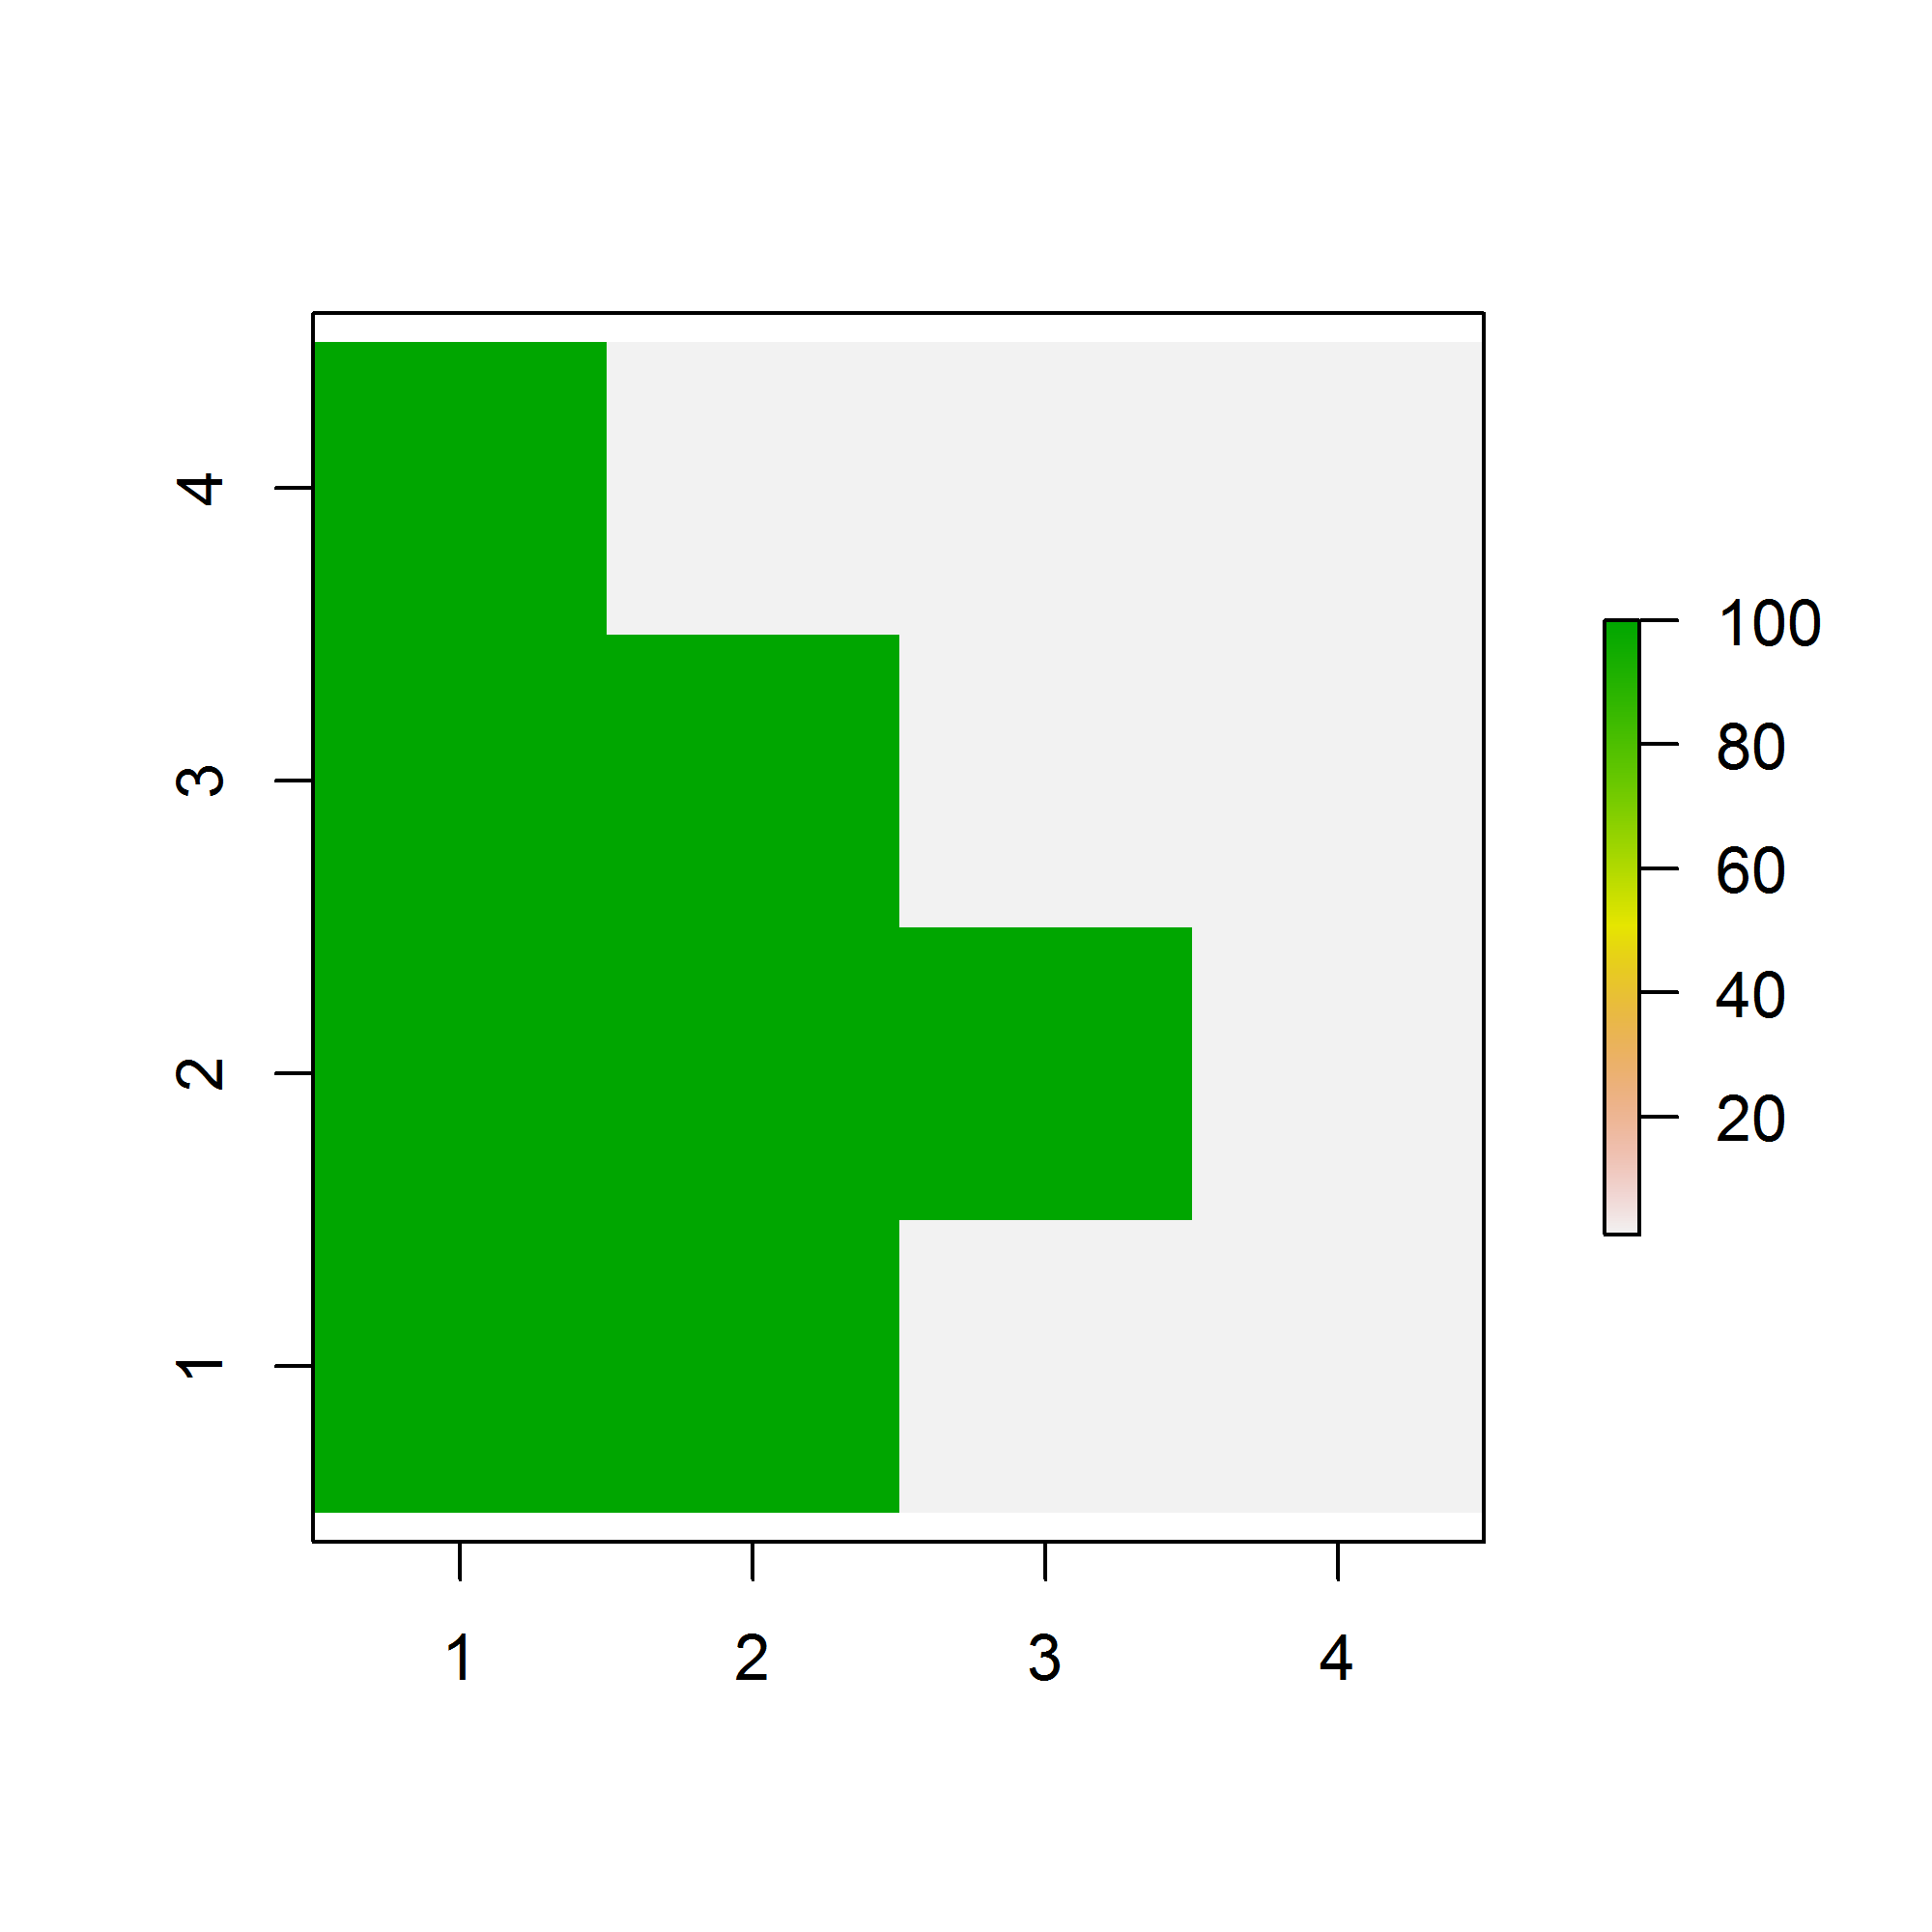
\includegraphics[height=3.25in,width=3.25in]{Ch10/figs/raster_2values}
\end{center}
\caption{A $4 \times 4$ raster with cost = 1 (white) or 100 (shaded) to represent ease of movement across a pixel.}
\label{ecoldist.fig.raster}
\end{figure}

Then we use the functions \mbox{\tt transition}, \mbox{\tt
  geoCorrection} (which doesn't really do anything if the coordinate system
  is UTM)
 and \mbox{\tt costDistance} to compute the distance
matrix. The transition function computes the cost of making a transition between
any two pixels, and it operates on the inverse-scale (''conductance'') and so the
\mbox{\tt transitionFunction} argument is given as $1/mean(x)$. 

To compute the cost distance we prescribe a set of points, or between
two sets of points (which is handy when one of the sets is of trap
locations, and the other is of individual activity centers).
To compute the distances for pixels in a raster, 
we use the center points of each raster.  The {\bf R}
 commands altogether are as follows:
{\small 
\begin{verbatim}
tr1<-transition(r,transitionFunction=function(x) 1/mean(x),directions=8)
tr1CorrC<-geoCorrection(tr1,type="c",multpl=FALSE,scl=FALSE)
pts<-cbind( sort(rep(1:4,4)),rep(4:1,4))
costs1<-costDistance(tr1CorrC,pts)
outD<-as.matrix(costs1)
\end{verbatim}
}
Now we can look at the result and see if it makes sense to us. Here we
print the first 5 columns of this distance matrix and illustration a
couple of examples of calculating the minimum cost-weighted distance
between points:
\begin{center}
{\small
\begin{verbatim}
> outD[1:5,1:5]
         1         2        3        4         5
1   0.0000 100.00000 200.0000 205.2426  50.50000
2 100.0000   0.00000 100.0000 200.0000  71.41778
3 200.0000 100.00000   0.0000 100.0000 171.41778
4 205.2426 200.00000 100.0000   0.0000 154.74264
5  50.5000  71.41778 171.4178 154.7426   0.00000
\end{verbatim}
} 
\end{center}
The interesting one is that between point 1 and 4. Note that simply
taking the shortest Euclidean distance, weighted by cost, produces a
cost-weighted distance of $100 \times 1$ to move from pixel 1 to pixel
2, and similarlly from 2 to 3 and 3 to 4, producing a total
cost-weighted distance of $300$. However, the actual {\it least-cost
  path} has cost-weighted distance $205.2426$. 
The shortest path has an individual moving from pixel 1 to 5, then 5
to 10, 10 to 15, 15 to 12, 12 to 8 and 8 to 4 which should add up to
$205.2426$.

\section{Fitting Models of Space Usage by MLE}
\label{ecoldist.sec.mle}

Throughout much of this book we rely on Bayesian analysis by MCMC mostly using 
{\bf BUGS}, but sometimes (as in Chapt. \ref{chapt.mcmc}) developing our own 
implementations. However, sometimes we prefer to use likelihood estimation, such as when
we can compare a set of models directly by likelihood either to do a
direct hypothesis test of a parameter, or tabulate a bunch of AIC values. It turns out, for this class
of models for space usage based on ecological distance, we actually prefer likelihood methods
not because they have any conceptual or methodological benefit, but simply because
they are more computationally efficient to implement \citep{royle_etal:2012ecol}.
So here we adopt our formulation of maximum likelihood estimation \citep{borchers_efford:2008} 
from Chapt. \ref{chapt.mle} 
for the class of models based on ecological distance. This is really just a straightforward
adaption of that.

We continue to work here with the binomial model:
\[
	y_{ij}| {\bf s}_{i} \sim \mbox{Bin}(K, p_{\theta}(d_{lcp}({\bf x}_{j},{\bf s}_{i};\theta_{2}); \theta_{0}, \theta_{1})
\]
where we have indicated the dependence of $p_{ij}$ on the parameters
${\bm \theta}$, and also $d_{lcp}$ which
itself depends on $\theta_{2}$, and the latent variable ${\bf s}$.
%The parameters
%${\bm \theta}$ include whatever parameters are involved in the
%cost-weighted distance function, i.e., at least $\theta_{2}$ from
%Eq. \ref{eq.cost}.
For the random effect we have ${\bf s}_{i} \sim  \mbox{Unif}({\cal
  S})$.
The joint distribution of the data for individual $i$ is the product
of $J$ binomial terms (i.e., contributions from each of $J$ traps):

\[
  [{\bf y}_{i} | {\bf s}_{i} , \theta] =
  \prod_{j=1}^{J} \mbox{Bin}(K, p_{\theta}({\bf x}_{j},{\bf s}_{i}) )
\]

{\flushleft This} assumes that encounter of individual $i$ in each
trap is independent of encounter in every other trap. Conditional on
${\bf s}_{i}$ this is reasonable in most applications in our view.
 The so-called marginal likelihood is computed by removing
${\bf s}_{i}$, by integration,  from the conditional-on-${\bf s}$
likelihood and regarding the {\it marginal} distribution of the data
as the likelihood. That
is, we compute:

\[
  [y|{\bm \theta}] =
\int_{{\cal S}}  [ {\bf y}_{i} |{\bf s}_{i},{\bm \theta}] g({\bf s}_{i}) d{\bf s}_{i}
\]

{\flushleft where}, under the uniformity assumption, we have
$g({\bf s}) = 1/||{\cal S}||$.
The joint likelihood for all $N$ individuals, assuming independence of
encounters among individuals, is the product of $N$ such terms:

\[
{\cal L}({\bm \theta} | {\bf y}_{1},{\bf y}_{2},\ldots, {\bf y}_{N}) = \prod_{i=1}^{N}
[{\bf y}_{i}|{\bm \theta}]
\]

The key operation for computing the likelihood is solving the
2-dimensional integration problem to remove ${\bf s}$, which we
resolve as we did previously in Chapt. \ref{chapt.mle}, using the
rectangular rule for integration, and averaging the integrand over a
fine mesh of points.
Therefore, 
the marginal pmf of ${\bf y}_{i}$, is
approximated by
\begin{equation}
         [{\bf y}_{i}|\theta] = \frac{1}{nG} \sum_{u=1}^{nG}  [ {\bf
            y}_{i} |{\bf s}_u, \theta]
\label{mle.eq.intlik}
\end{equation}

To deal with the fact that $N$ is unknown, there are two key issues
that need to be addressed.  First is that we don't observe the
``all-zero'' encounter histories (i.e., $y_{ij} = 0$ for all $j$)
corresponding to uncaptured individuals, so we have to make sure we
compute the probability for that all zero encounter history which we
do operationally by tacking a row of zeros onto the encounter history
matrix. We include the number of such all-zero encounter histories as
an unknown parameter of the model, which we label $n_{0}$.  In
addition, we have to be sure to include a combinatorial term to
account for the fact that of the $n$ observed individuals there are
${N \choose n}$ ways to realize a sample of size $n$. The
combinatorial term involves the unknown $n_{0}$ and thus it must be
included in the likelihood.

We wrote an {\bf R} function to evaluate the likelihood which we optimize
using the {\bf R} function \mbox{\tt nlm}.
The likelihood is given in the {\tt scrbook} package as the function
\mbox{\tt intlik3ed}. The help file 
provides an example of its usage and for simulating data.

To use this function the cost covariate $z(x)$ has to be of class 
\mbox{\tt RasterLayer} which requires packages \mbox{\tt sp} and
\mbox{\tt raster} to manipulate. 
The following is a stylized and more concise verstion of the actual
function, and we apply this in the following section.

{\small
\begin{verbatim}
intlik3ed<-function(start=NULL,y=y,K=NULL,X=traplocs,
distmet="ecol",covariate,theta2=NA){

nc<-covariate@ncols
nr<-covariate@nrows
Xl<-covariate@extent@xmin
Xu<-covariate@extent@xmax
Yl<-covariate@extent@ymin
Yu<-covariate@extent@ymax
### ASSUMES SQUARE RASTER -- NEED TO GENERALIZE THIS
delta<- (Xu-Xl)/nc
xg<-seq(Xl+delta/2,Xu-delta/2,delta) 
yg<-seq(Yl+delta/2,Yu-delta/2,delta) 
npix.x<-length(xg)
npix.y<-length(yg)
area<- (Xu-Xl)*(Yu-Yl)/((npix.x)*(npix.y))
G<-cbind(rep(xg,npix.y),sort(rep(yg,npix.x)))
nG<-nrow(G)

if(distmet=="euclid")
D<- e2dist(X,G)  
if(distmet=="ecol"){
if(is.na(theta2))
theta2<-exp(start[4])
cost<- exp(theta2*covariate)
tr1<-transition(cost,transitionFunction=function(x) 1/mean(x),directions=8)
tr1CorrC<-geoCorrection(tr1,type="c",multpl=FALSE,scl=FALSE)
D<-costDistance(tr1CorrC,X,G)
}

theta0<-start[1]; theta1<-start[2]; n0<-exp(start[3])

probcap<- (exp(theta0)/(1+exp(theta0)))*exp(-theta1*D*D)
Pm<-matrix(NA,nrow=nrow(probcap),ncol=ncol(probcap))
ymat<-y ; ymat<-rbind(y,rep(0,ncol(y)))
lik.marg<-rep(NA,nrow(ymat))
for(i in 1:nrow(ymat)){
Pm[1:length(Pm)]<- (dbinom(rep(ymat[i,],nG),rep(K,nG),probcap[1:length(Pm)],log=TRUE))
lik.cond<- exp(colSums(Pm))
lik.marg[i]<- sum( lik.cond*(1/nG) )  
}                                                 
nv<-c(rep(1,length(lik.marg)-1),n0)
part1<- lgamma(nrow(y)+n0+1) - lgamma(n0+1)
part2<- sum(nv*log(lik.marg))
out<-  -1*(part1+ part2)
out
}
\end{verbatim}
}

\subsection{Bayesian Analysis}

It is difficult to fit these models using the {\bf BUGS} engines
because it is not possible, to the best of our knowledge, to compute
the least-cost path distance.  It would be possible to fit the models
in {\bf BUGS} if the parameter $\theta_{2}$ was fixed. In that case,
one could compute the distance matrix ahead of time and reference the
required elements for a given ${\bf s}$.
Alternatively, it would be possible to write a custom MCMC routine
using the methods we present in Chapt. \ref{chapt.mcmc}, although we
have not yet developed our own implementation.




\section{Example: SCR model based on ecological distance}

In this section we provide examples that we think are typical of how
cost-weighted distance models can be used in real capture-recapture
problems.  We define a $20 \times 20$ pixel covariate raster with
extent = $[0.5, 4.5] \times [0.5, 4.5]$.  We regard this, for the
purposes of our example, as a coarse landscape covariate, with pixels
having some arbitrary scaling say, a $2 \times 2$ km resolution. Thus,
the raster defines a landscape of $40 \times 40$ km and we suppose
that 16 camera traps are established at the integer coordinates
$(1,1), (1,2), \ldots, (4,4)$. We could think of this as a landscape
within which we're studying a population of ocelots, lynx or some
other cat.

For our analyses, cost is characterized by a single covariate raster
and we consider two specific cases. First is an increasing trend from
the NW to the SE (''systematic raster''), where $z(x)$ is defined as
$z(x) = r(x) + c(x)$ where $r(x)$ and $c(x)$ are just the row and
column, respectively, of the raster.  This might define something
related to distance from an urban area or a gradient in habitat
quality due to land use, or environmental conditions such as
temperature or precipitation gradients.  In the second case we make up
a covariate by generating a field of spatially correlated noise to
emulate a typical patchy habitat covariate (''patchy raster'') such as
tree or understory density. The two covariates are shown in
Fig. \ref{ecoldist.fig.raster100}, along with a sample realization of
$N=100$ individuals (left panel only).  For both covariates we use a
cost function in which transitions from pixel ${\bf x}$ to ${\bf x}'$
is given by:

\[
 log(cost({\bf x},{\bf x}'))=  \theta_2 \frac{z({\bf x}) + z({\bf x}')}{2}
\]

{\flushleft where} $\theta_2 = 1$ for simulating the observed data.
 With $\theta_2=0$ then the
model reduces to one in which the cost of moving across each pixel is
constant, and therefore Euclidean distance is operative.

\begin{figure}
\begin{tabular}{cc}
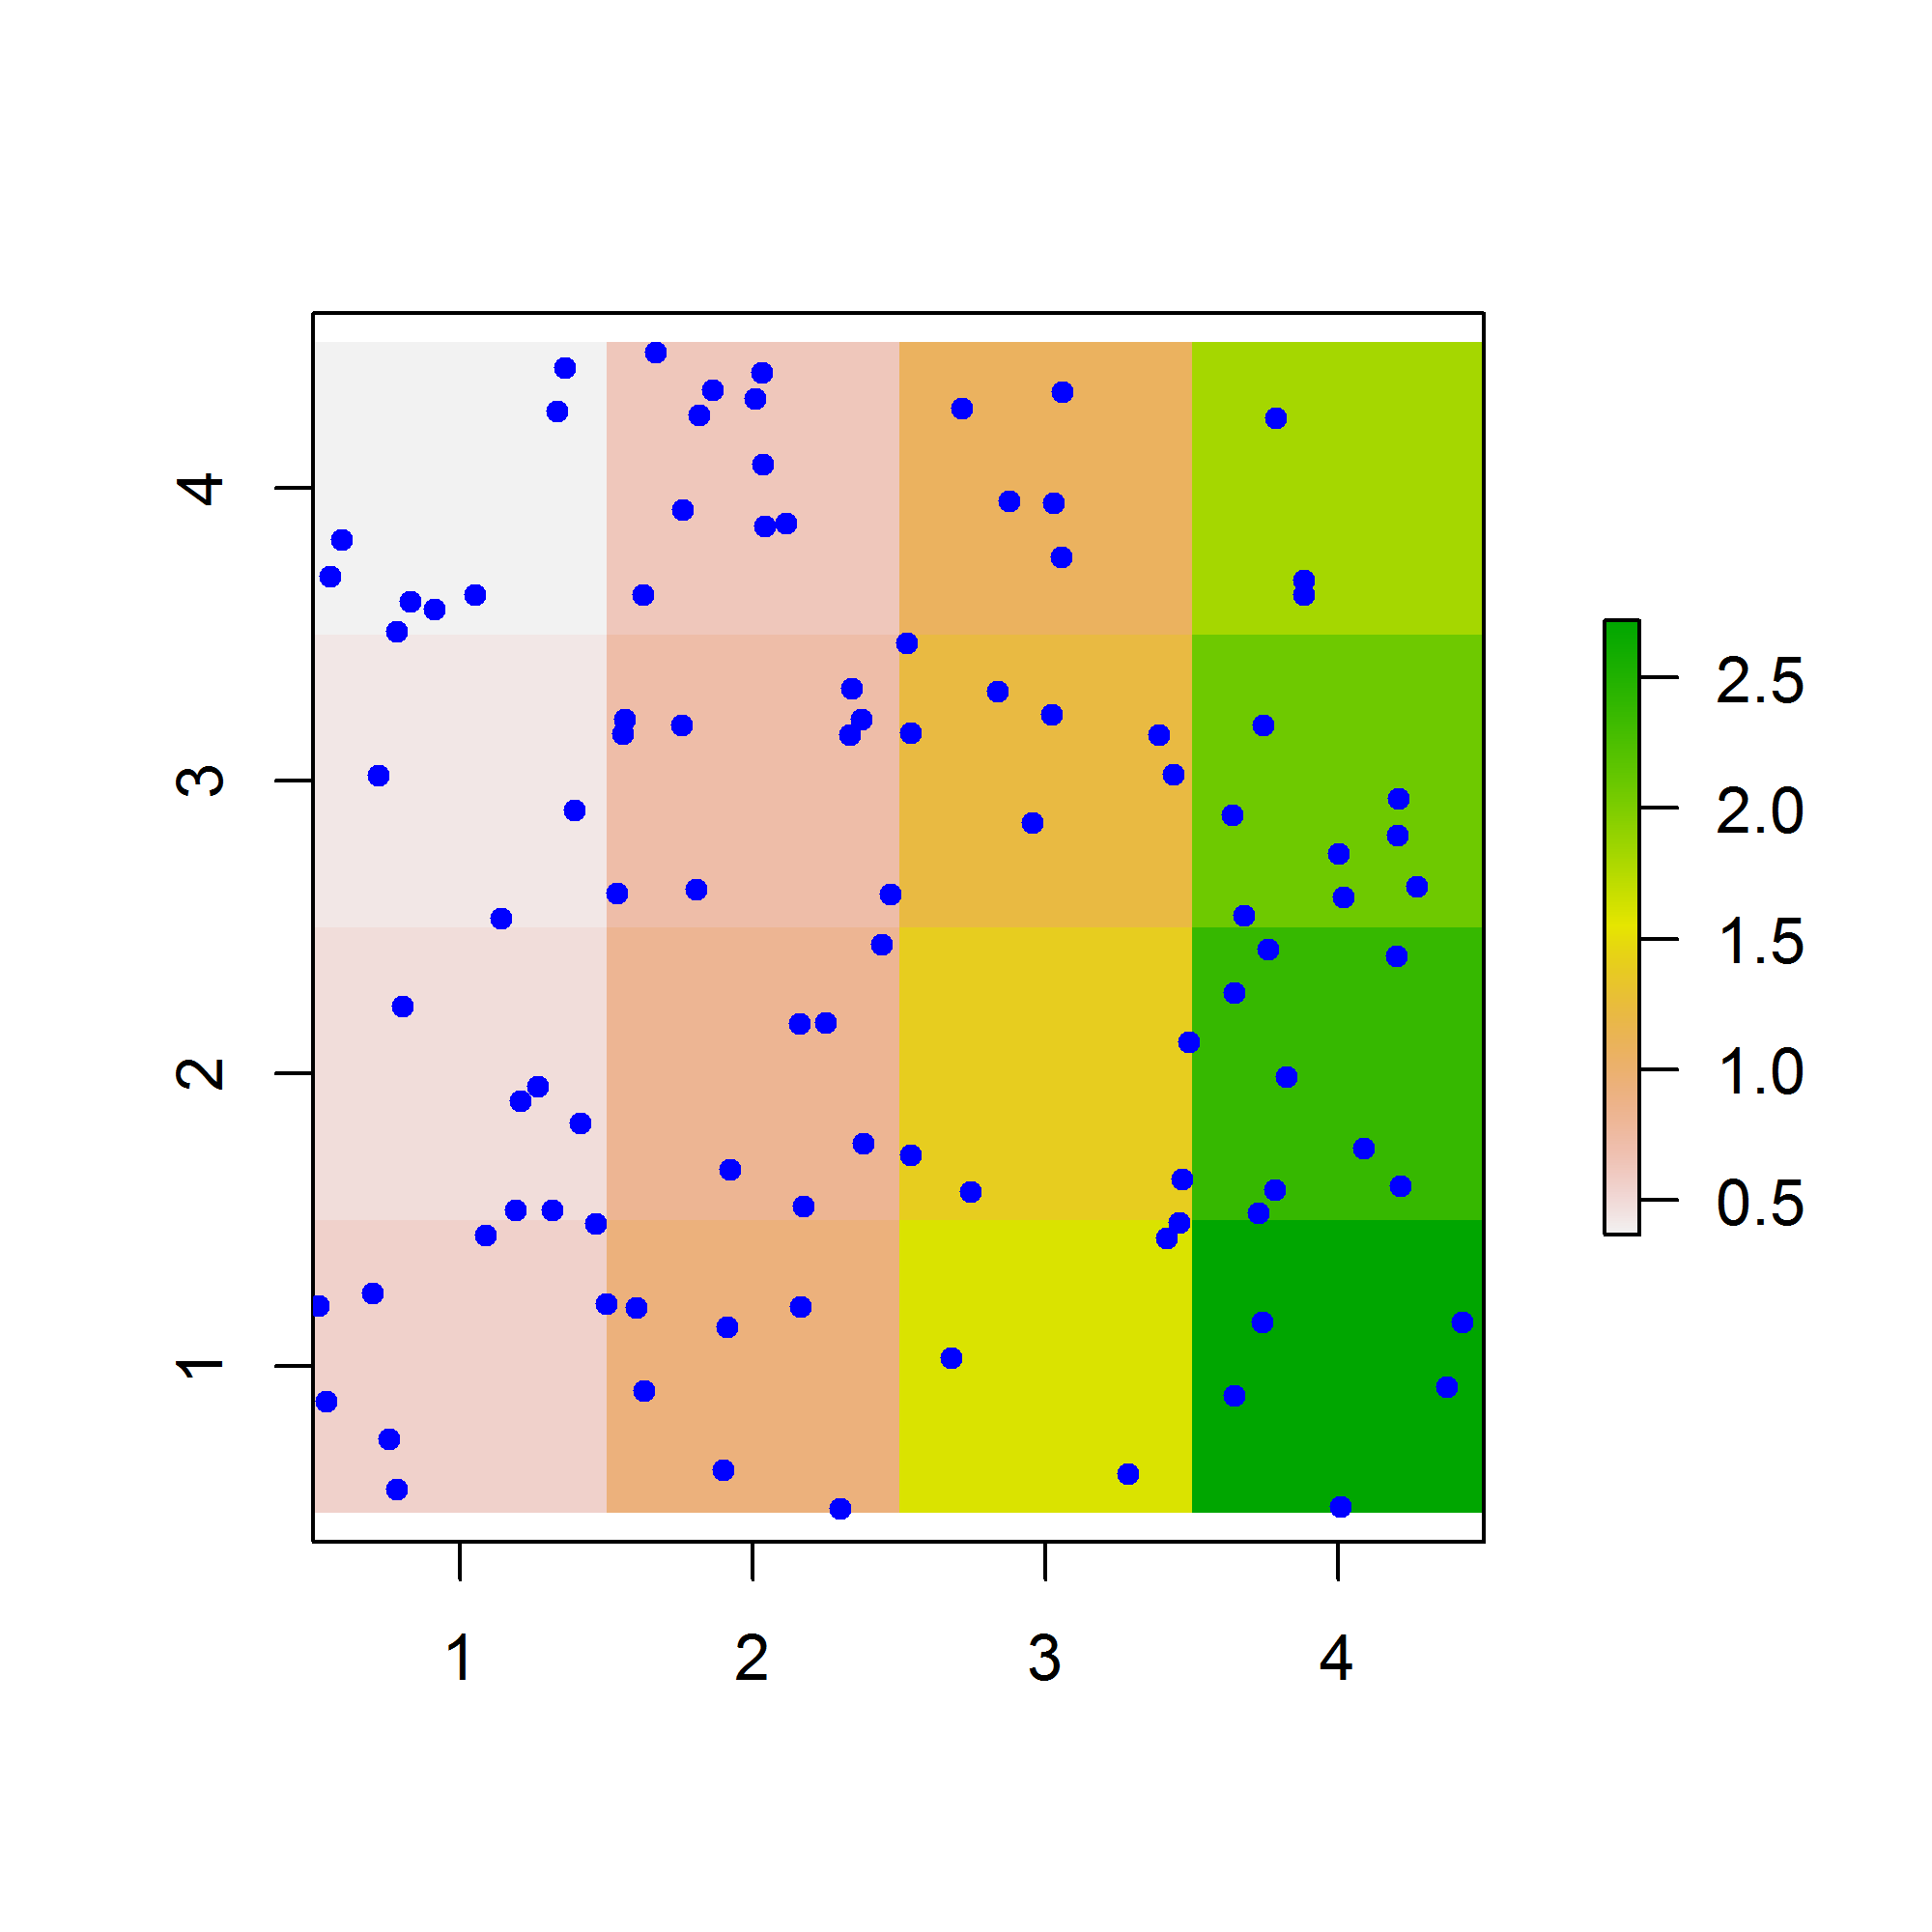
\includegraphics[height=3.25in,width=3.25in]{Ch10/figs/raster_withN100}
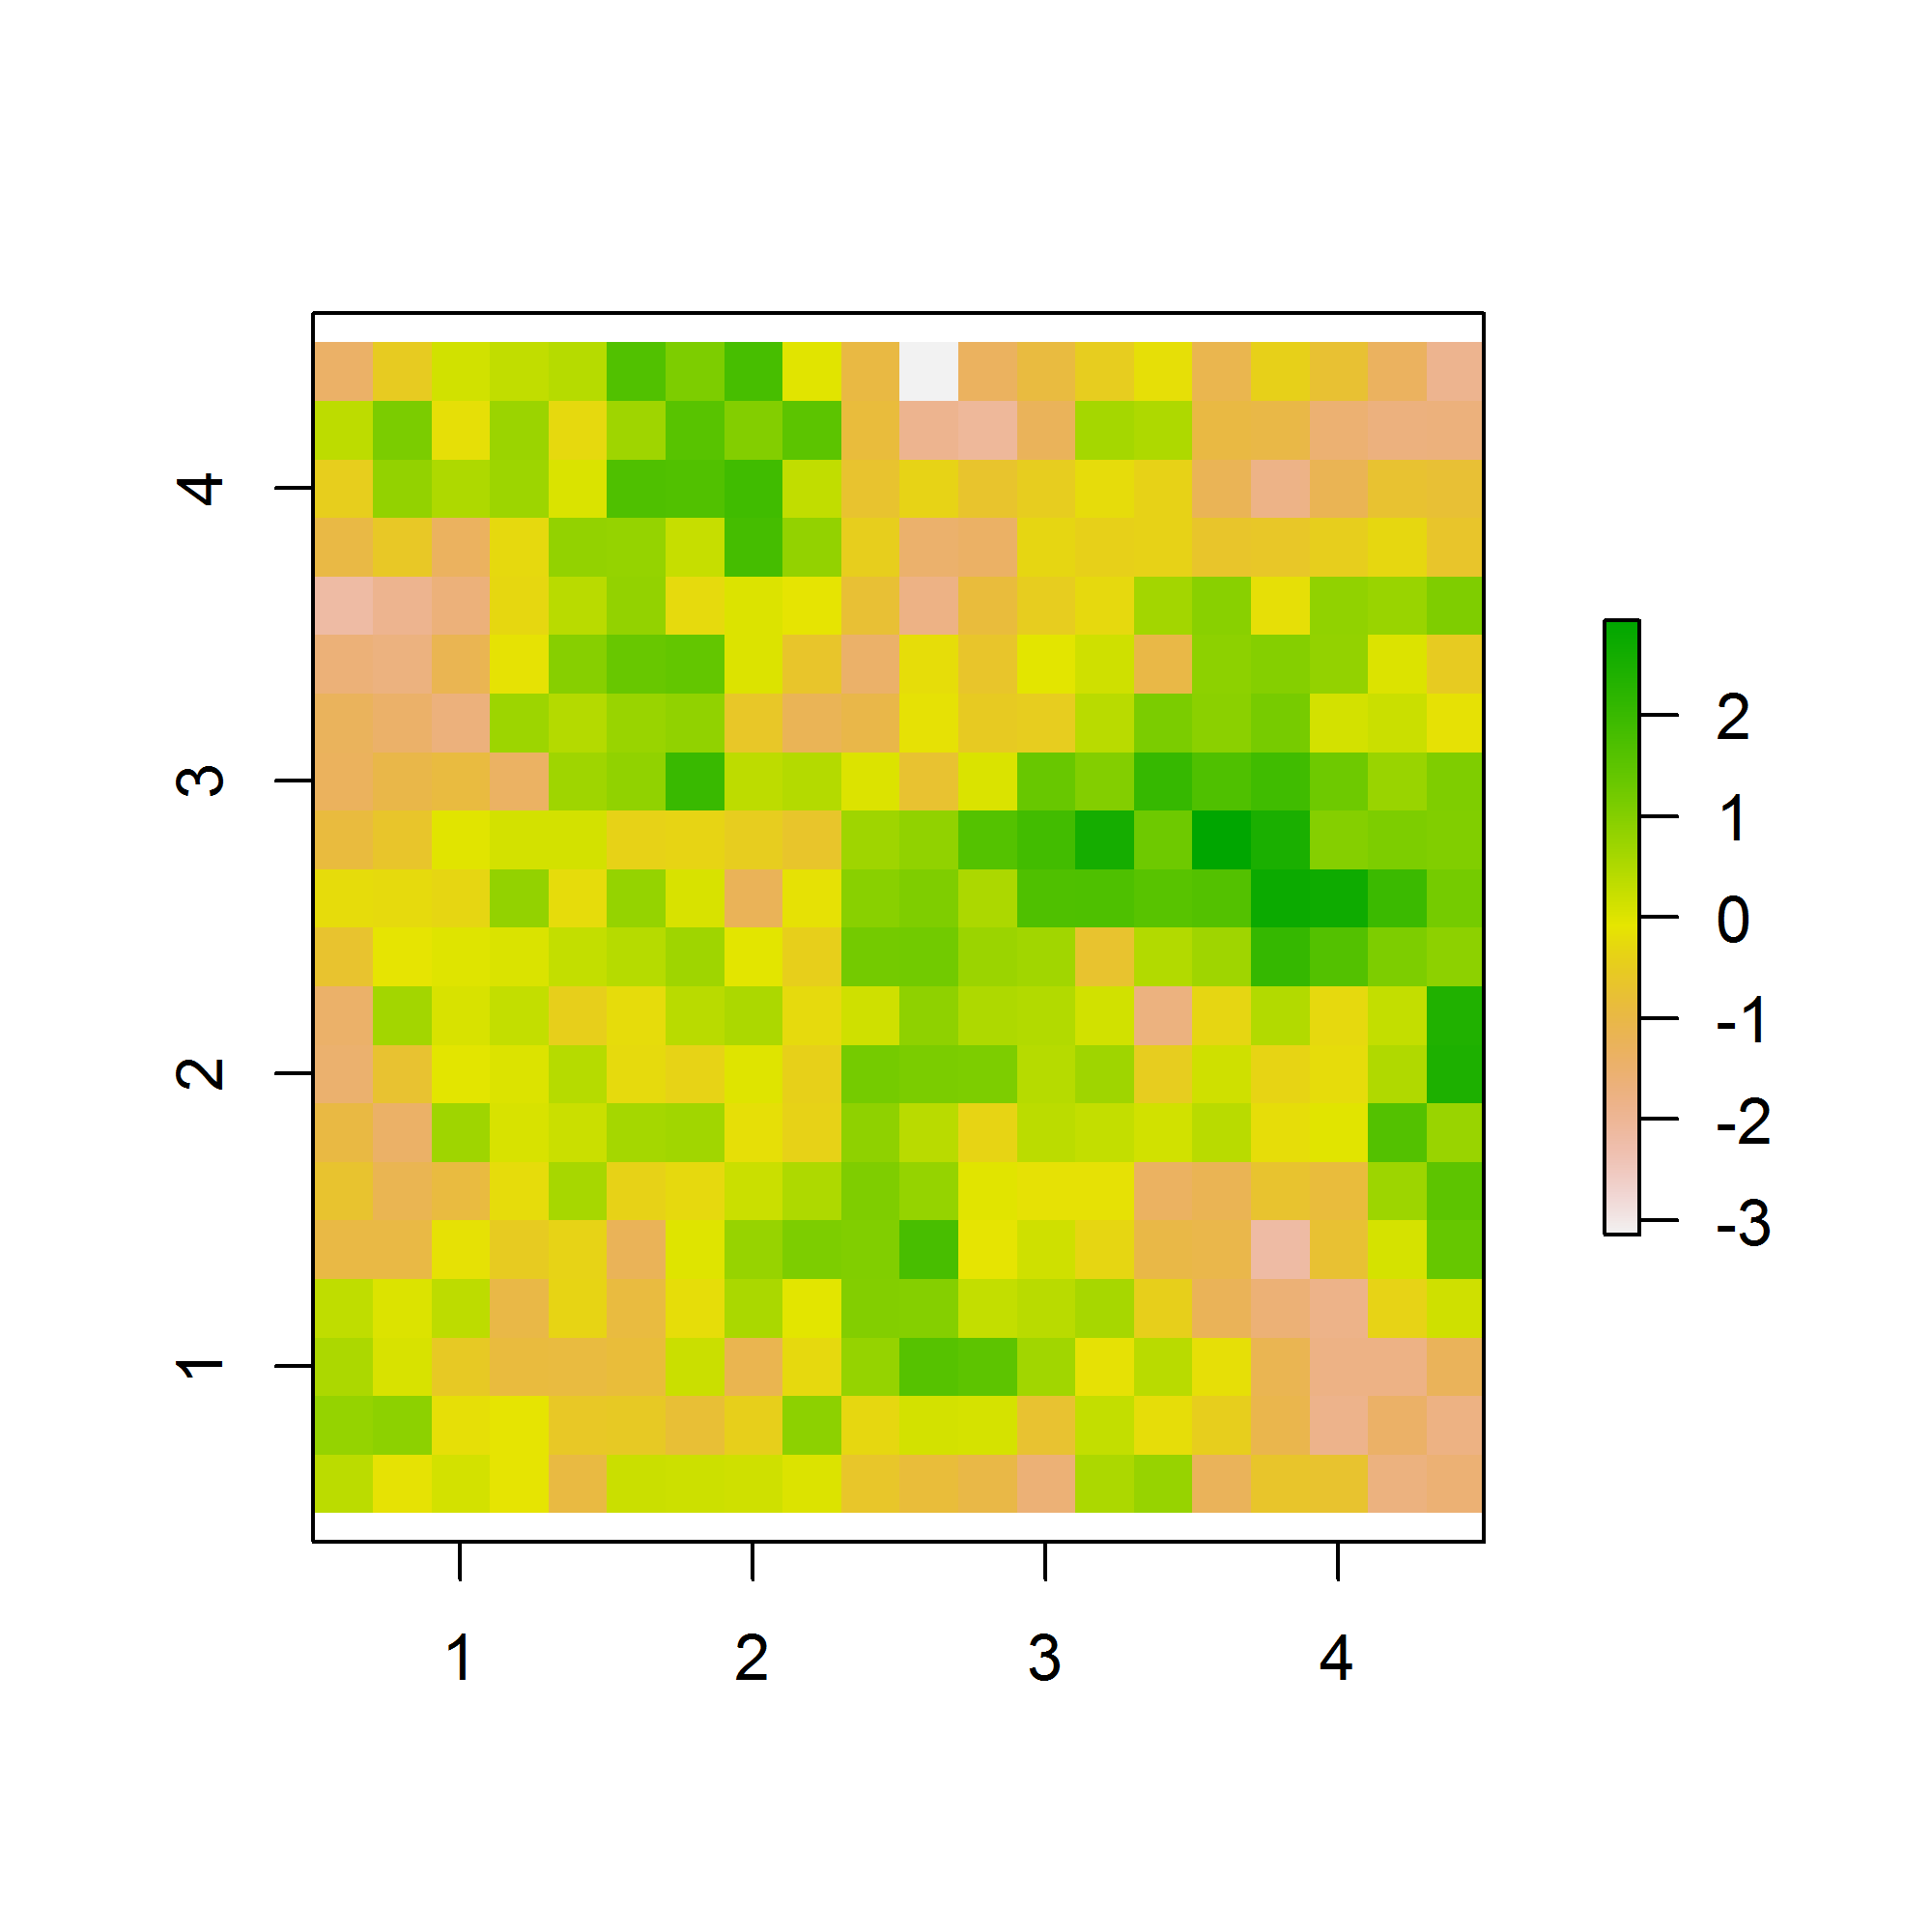
\includegraphics[height=3.25in,width=3.25in]{Ch10/figs/raster_krige} &
\end{tabular}
\caption{Two covariate rasters used for simulations. A hypothetical
  realization of $N=100$ activity centers is superimposed on the left,
along with 16 trap locations. }
\label{ecoldist.fig.raster100}
\end{figure}

\subsection{Non-stationarity of home range structure}

When distance is defined by the cost-weighted distance metric given
by Eq. \ref{eq.lcp} then individual space-usage varies
spatially in response to the landscape covariate(s) used in the
distance metric. For example, using one of the covariates we use in
our simulation study below (Fig. \ref{ecoldist.fig.raster100}, right
panel) with a Gaussian pdf detection function but having distance
metric defined by Eq. \ref{eq.lcp}, produces home ranges such
as those shown in Fig. \ref{fig.homeranges}. Later we simulate data
under the model that produces these home ranges and fit spatial
capture-recapture models to evaluate the efficacy of likelihood
estimation under this model.

\begin{figure}
\begin{center}
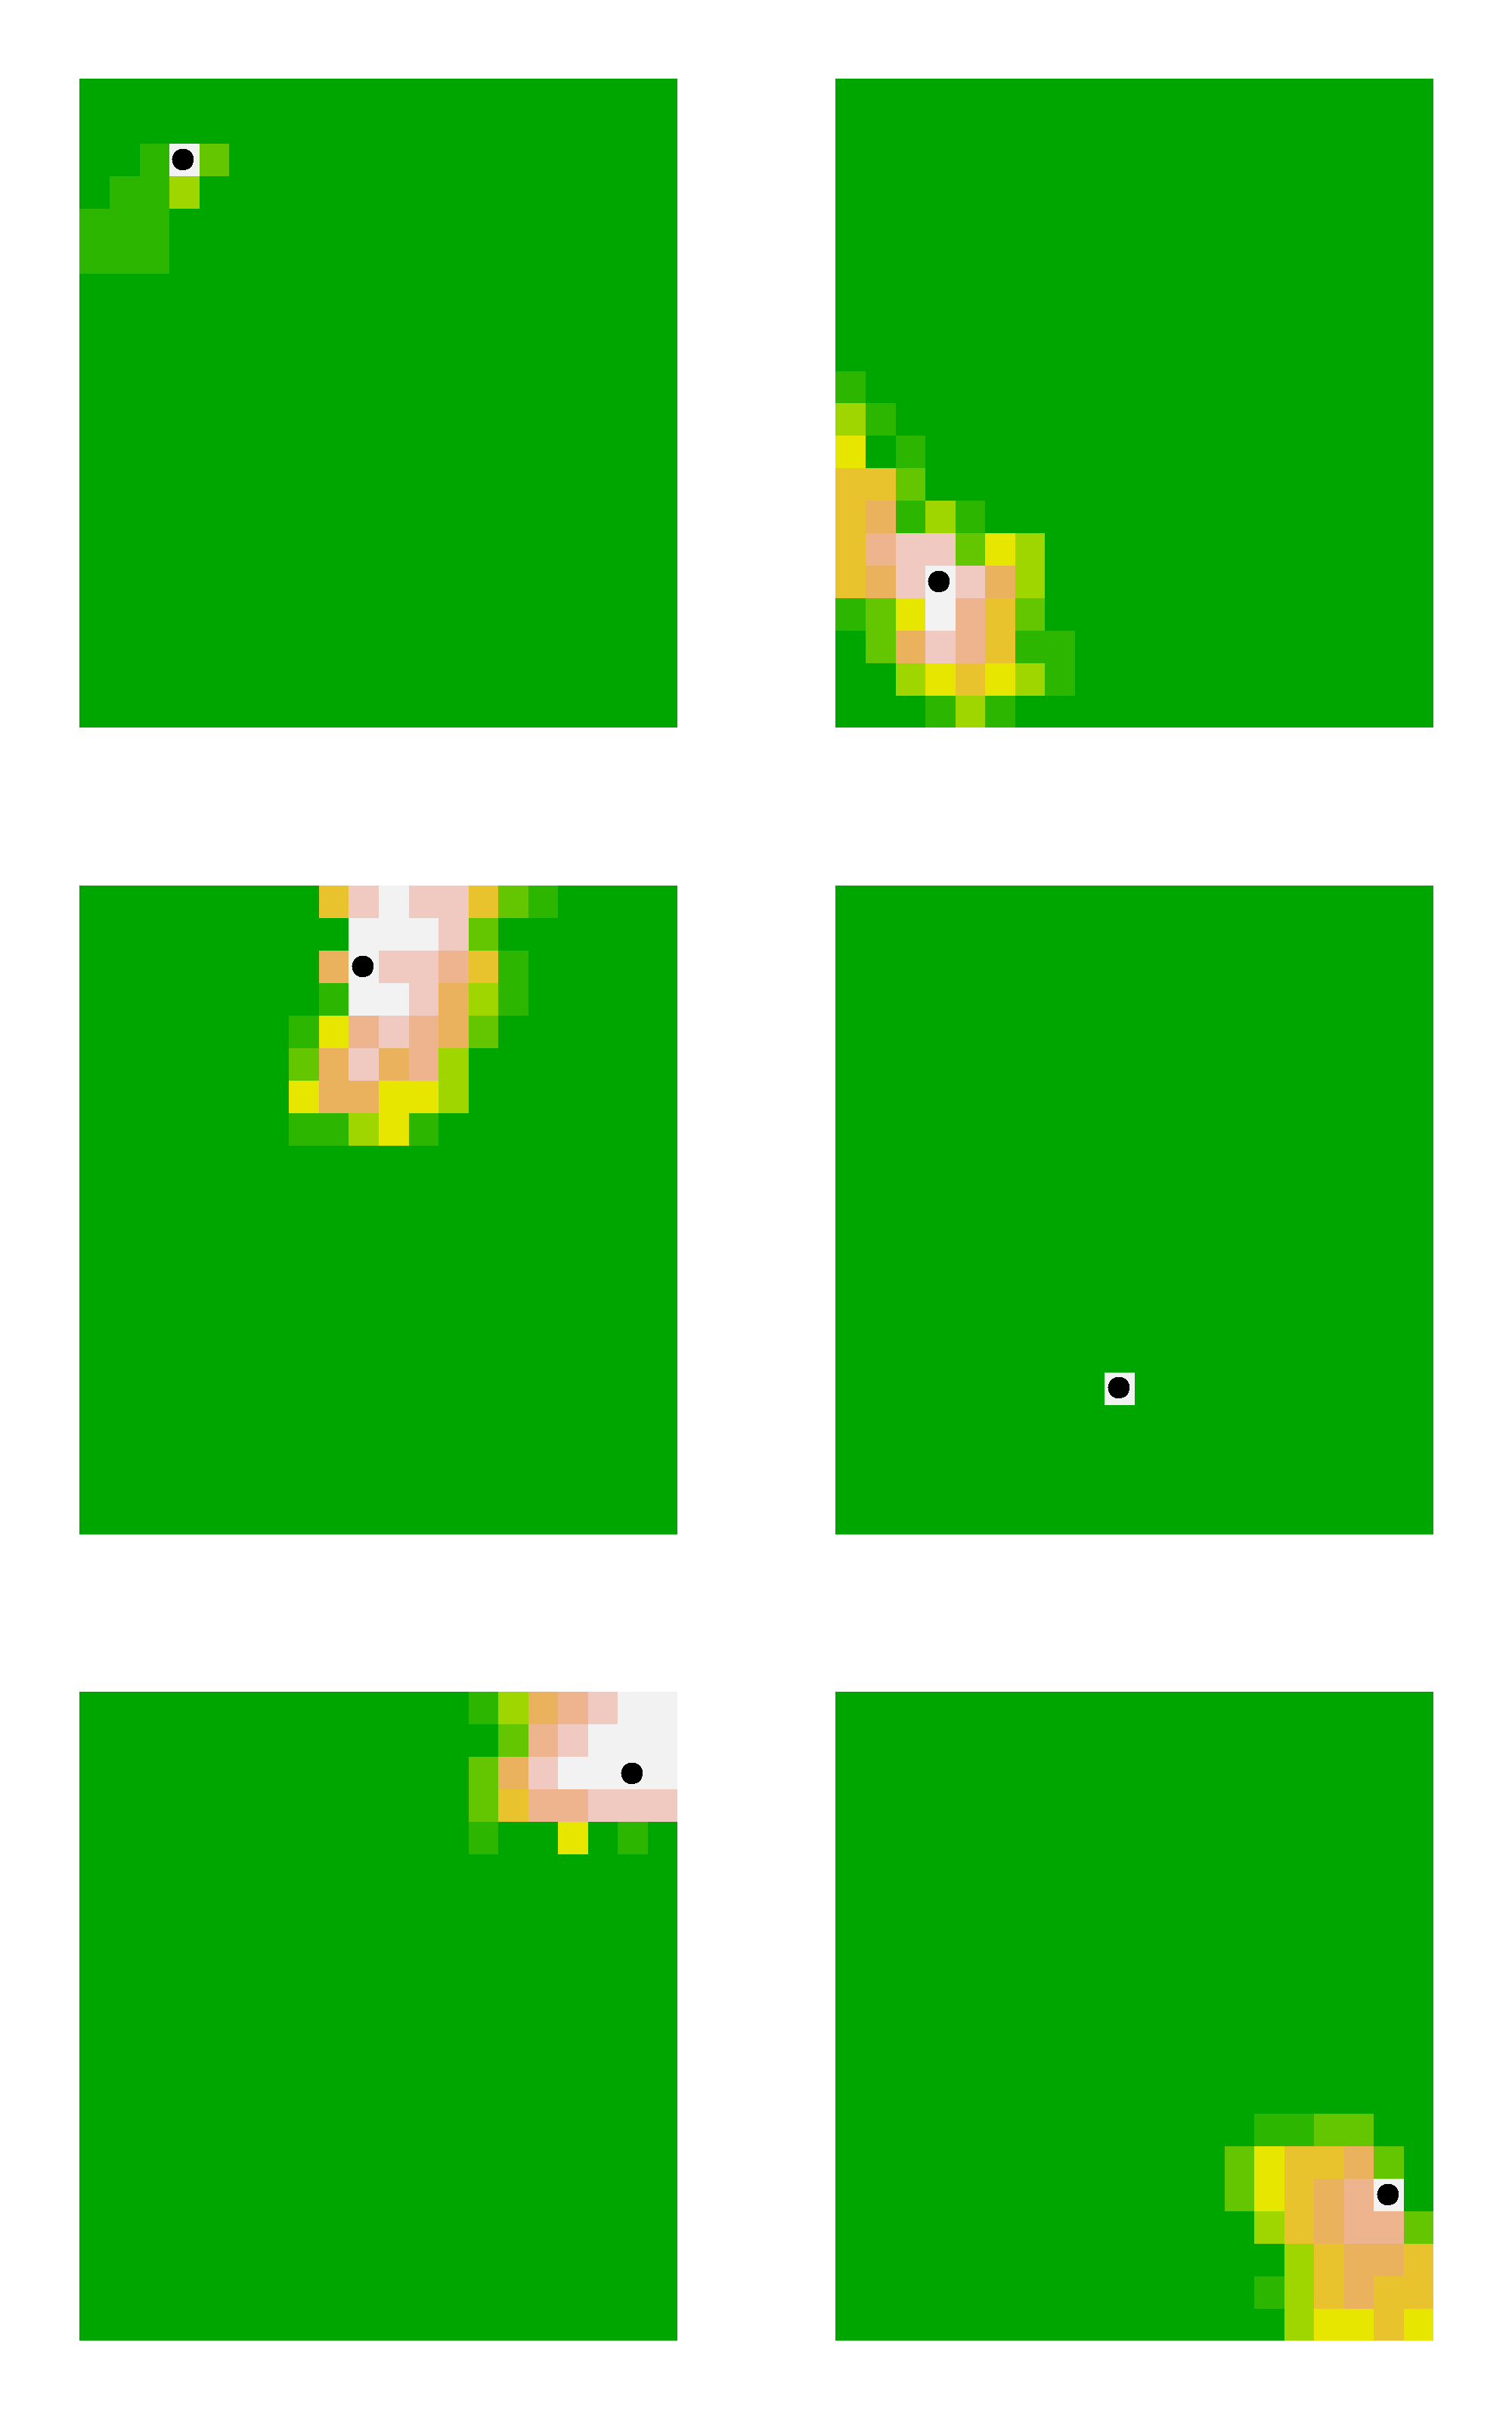
\includegraphics[height=6in,width=3.75in]{Ch10/figs/home_ranges}
\end{center}
\caption{
Typical home ranges for 6 individuals based on the cost surface shown in
  Fig. \ref{ecoldist.fig.raster100} with $\theta_{2}=1$. The black dot indicates the home
  range center and the pixels around each home range center are shaded
according to the probability of encounter, if a trap were located in
that pixel.
}
\label{fig.homeranges}
\end{figure}


\subsection{Simulation and Analysis}

We begin by simulating some data... we have to load the scrbook
library and grab some covariates...............

{\small 
\begin{verbatim}
library("scrbook")
out<-make.EDcovariates()
covariate<-out$covariate.patchy
set.seed(2013)

N<-200
theta0<- -2
sigma<- .5
K<- 5

theta1<- 1/(2*sigma*sigma)
r<-raster(nrows=20,ncols=20)
projection(r)<- "+proj=utm +zone=12 +datum=WGS84"
extent(r)<-c(.5,4.5,.5,4.5)
theta2<-1
cost<- exp(theta2*covariate)

tr1<-transition(cost,transitionFunction=function(x) 1/mean(x),directions=8)
tr1CorrC<-geoCorrection(tr1,type="c",multpl=FALSE,scl=FALSE)

# make up some trap locations
xg<-seq(1,4,1)
yg<-4:1
pts<-cbind( sort(rep(xg,4)),rep(yg,4))

traplocs<-pts
points(traplocs,pch=20,col="red")
ntraps<-nrow(traplocs)

S<-cbind(runif(N,.5,4.5),runif(N,.5,4.5))
D<-costDistance(tr1CorrC,S,traplocs)
probcap<-plogis(theta0)*exp(-theta1*D*D)
# now generate the encounters of every individual in every trap
Y<-matrix(NA,nrow=N,ncol=ntraps)
for(i in 1:nrow(Y)){
 Y[i,]<-rbinom(ntraps,K,probcap[i,])
}
Y<-Y[apply(Y,1,sum)>0,]

n0<- N-nrow(Y)
frog1<-nlm(intlik3ed,c(theta0,theta1,log(n0)),hessian=TRUE,y=Y,K=K,X=traplocs,
               distmet="euclid",covariate=covariate,theta2=1)

frog2<-nlm(intlik3ed,c(theta0,theta1,log(n0),-.3),hessian=TRUE,y=Y,K=K,X=traplocs,
               distmet="ecol",covariate=covariate,theta2=NA)
\end{verbatim}
}

Comment on the difference.......


\subsection{Simulation study}

We devised a limited simulation study to evaluate three things: (1)
the general statistical performance of the density estimator under
this new model; (2) the effect of mis-specifying the model with a
normal Euclidean distance metric and (3) the statistical performance
of estimating the relative cost parameter.

We used population sizes of 100 and 200 individuals with activity
centers randomly distributed on the $20 \times 20$ landscape, and subjected them
to encounter by 16 traps arranged in a $4\times 4$ grid according to
the Euclidean distance metric. We fit 3 different models; (i) the
misspecified euclidean distance model; (ii) the true data-generating
model with the relative cost raster {\it known} and (iii) the true
data-generating model but estimating the relative cost parameter by
maximum likelihood.  We used the ``systematic'' and ``patchy''
covariates defined previously.

We simulated encounter data for the $N$ individuals using the Gaussian
encounter model with least-cost path distance metric:

\[
log(p_{ij})= \theta_{0} + \theta_{1} d_{lcp}({\bf x}_{j},{\bf
  s}_{i}; \theta_{2})^{2}
\]

{\flushleft We } used here $\theta_{0} = -2$ and $\theta_{1} = 2$, the latter value
corresponding to $\sigma = 0.5$ of a stationary bivariate normal home
range model.  We varied the number of replicate samples $K=3,5,10$
(e.g., nights in a camera trapping study) to produce varying sample
sizes.  Because any simulation study is inherently arbitrary, we have
provided {\bf R} scripts for carrying out simulations in Appendix 2 so
that the interested reader can experiment with their own situations.
















































\subsection{Simulation Results}

For both landscapes and all simulation conditions (levels of $K$ and
$N$) the average sample sizes of individuals captured are given in
Tab. \ref{tab.samplesize}.  The simulation results for estimating $N$
for the prescribed state-space are presented in Table
\ref{tab.results1} 2 below.  For the ``patchy'' landscape we see extreme
bias in estimates of $N$ when the Euclidean distance is used. There is
moderate small sample bias of 3-5\% in the MLE of $N$ using the
least-cost distance which becomes negligible as $K$ increases. For
$N=200$ the bias is on the order of 2\% for the lowest sample size
case ($K=3$) but negligible otherwise.  Interestingly, for the
landscape exhibiting systematic structure, there is a persistent bias
in the MLE of $N$ of 1-3\% even for the highest level of $K$. We were
initially surprised by this but, in fact, it is due to the fact that
the state-space is small relative to the extent of the trap grid and
sensitivity to a state-space that is too small is expected because the
support of the integrand is truncated. In the particular case of the
systematic landscape, we find that, in the NW corner of the raster
where cost of movement is low, individuals use large areas of space,
and the fitted model is under-stating the apparent
heterogeneity in encounter probability for the prescribed raster.  We
found that the issue is resolved when the traps are moved away from
the boundary (see Appendix 3).

The performance of estimating the cost parameter $\theta_{2}$ mirrors
the results for estimating $N$ for the prescribed state space. In the
patchy landscape where we don't expect a systematic gradient in space
usage around the edge of the state-space, we see
(Table \ref{tab.results2}) that $\theta_{2}$ is estimated with
diminishing bias as the sample size increases, but with persistent
bias due to truncation of the likelihood under the systematic
landscape which, as with the MLE of $N$, is resolved by moving the
traps away from the edge of the raster. Equivalently, in practice,
this could be resolved by expanding the raster away from the trap
locations so that all regions used by animals exposed to capture are
included in the state-space.



\begin{table}[htp]
\centering
\caption{
Expected sample sizes of captured individuals under each configuration of
$N$ (population size for the prescribed state-space) and $K$ (number of replicate samples).
}
\begin{tabular}{l|rrrr}
 & \multicolumn{2}{c}{Systematic} & \multicolumn{2}{c}{Patchy}  \\
    & N=100 &  N=200  &   N=100 &  N=200  \\ \hline
K=3 &  38.69 &   78.17  &   37.30 &   74.93  \\
K=5 &  51.10 &  103.18  &   51.89 &  103.71 \\
K=10&  65.81 &  132.39  &   69.44 &  138.76 \\
\end{tabular}
\label{tab.samplesize}
\end{table}



\begin{table}[htp]
\centering
\caption{
Mean of sampling distribution of the cost function parameter
$\theta_{2}$ for the different simulation
conditions. 
}
\begin{tabular}{l|rrrr}
 & \multicolumn{2}{c}{Patchy} & \multicolumn{2}{c}{Systematic} \\
    & N=100 &  N=200  &   N=100 &  N=200  \\ \hline
K=3 &   1.05&    1.03 &     1.17 & 1.14 \\
K=5 &   1.02&    1.01 &     1.12 &1.12 \\
K=10&   1.01&    1.00 &     1.10 &1.08 \\
\end{tabular}
\label{tab.results2}
\end{table}





\section{Illustration: Example Good vs. Bad habitat}

We provide another illustration of how to employ ecological distance
calculations in SCR models. This example shows more GIS-like analysis
for a situation where we have something like a hard habitat boundary
created to mimic a habitat corridor or park unit or some other block
of relatively homogeneous good-quality habitat for some species. This
particular system (shown in Fig. \ref{ecoldist.fig.corridor}), could
be habitat surrounded by a suburban wasteland of McDonalds and
Wal-Marts, much less hospital habitat for most species.  For our
purposes, we suppose that individuals live within the buffered ``f''
shaped region, although we could also imagine the negative of the
situation in which individuals live outside of the region, so that the
polygon represents a barrier (a lake) or bad habitat (an urban area)
or similar.  We describe the steps for creating this landscape
shortly, so that the reader can use a similar process to generate more
relevant landscapes for their own problems.

In this case we're not going to estimate any parameters of the cost
function (though we could) but instead we're going to use ecological
distance ideas only to constrain movement within (or to avoid)
landscape features.  However, the reader is encouraged to adapt the
likelihood function given in the previous section for this specific
case. 

\subsection{Basic Geographic Analysis in R}

In practical applications our landscape will contain one more more
polygons which delineate good or bad habitat or other important
characterisetics of the landscape.  These might exist as GIS
shapefiles or merely as a text file with coordinates defining polygon
boundaries. To work with polygons in the context of SCR models we need
to create a raster, overly the polygon and assign values to each pixel
depending on whether pixels are in the polygon or not, or how far they
are from polygon boundaries. These operations are relatively easy to
do within a GIS system but we need to be able to do them in ${\bf R}$
and we develop methods for this here.  See also
Chapts. \ref{chapt.mle} and \ref{chapt.mcmc} XXX exact sections ??
XXXX for examples of reading in the shapefile and using them to affect
calculations in SCR models.

The first thing we do here is create a set of polygons that arise by
buffering and joining some line segments.
In the {\bf R} library \mbox{\tt scrbook}, we provide 
 a function \mbox{\tt make.seg} which allows the user to make such
 lines segments given a 
specific trap region.  To involve \mbox{\tt make.seg} we first
creating a plot region and then call \mbox{\tt make.seg} which has a
single argument being the number of points used to define the line
segment. In the following set of commands we generate two line
segments, \mbox{\tt l1} consisting of 9 points and \mbox{\tt l2}
consisting of 5 points, and these reside in a geographic region
enclosedd by $[0,10] \times [0,10]$:
{\small 
\begin{verbatim}
library("scrbook")
library("sp")
plot(NULL,xlim=c(0,10),ylim=c(0,10))
l1<-make.seg(9)
plot(l1)
l2<-make.seg(5)
plot(l1)
lines(l2)
\end{verbatim}
}

We used this function to create a couple of line segments of class
\mbox{\tt SpatialLines} from the {\bf R} package \mbox{\tt sp}, which
can be loaded from \mbox{\tt scrbook} as  follows
\begin{verbatim}
data("fakecorridor")
\end{verbatim}
This has 2 line files in it (\mbox{\tt l1} and \mbox{\tt l2}) and a
trap locations file (\mbox{\tt traps}). 
We use some functions from the {\bf R} packages \mbox{\tt sp} and
\mbox{\tt rgeos} to join and 
buffer (by 0.5 units) the two segments. The commands are as follows
and the result is shown in Fig. \ref{ecoldist.fig.corridor}.

{\small
\begin{verbatim}
data("fakecorridor")
library("sp")
library("rgeos")

l1<-l1.old
l2<-l2.old
buffer<- 0.5
par(mfrow=c(1,1))
aa<-gUnion(l1,l2)
plot(gBuffer(aa,width=buffer),xlim=c(0,10),ylim=c(0,10))
pg<-gBuffer(aa,width=buffer)
pg.coords<- pg@polygons[[1]]@Polygons[[1]]@coords

xg<-seq(0,10,,40)
yg<-seq(10,0,,40)

delta<-mean(diff(xg))
pts<- cbind(sort(rep(xg,40)),rep(yg,40))
points(pts,pch=20)

in.pts<-point.in.polygon(pts[,1],pts[,2],pg.coords[,1],pg.coords[,2])
points(pts[in.pts==1,],pch=20,col="red")
\end{verbatim}
}


\begin{figure}
\begin{center}
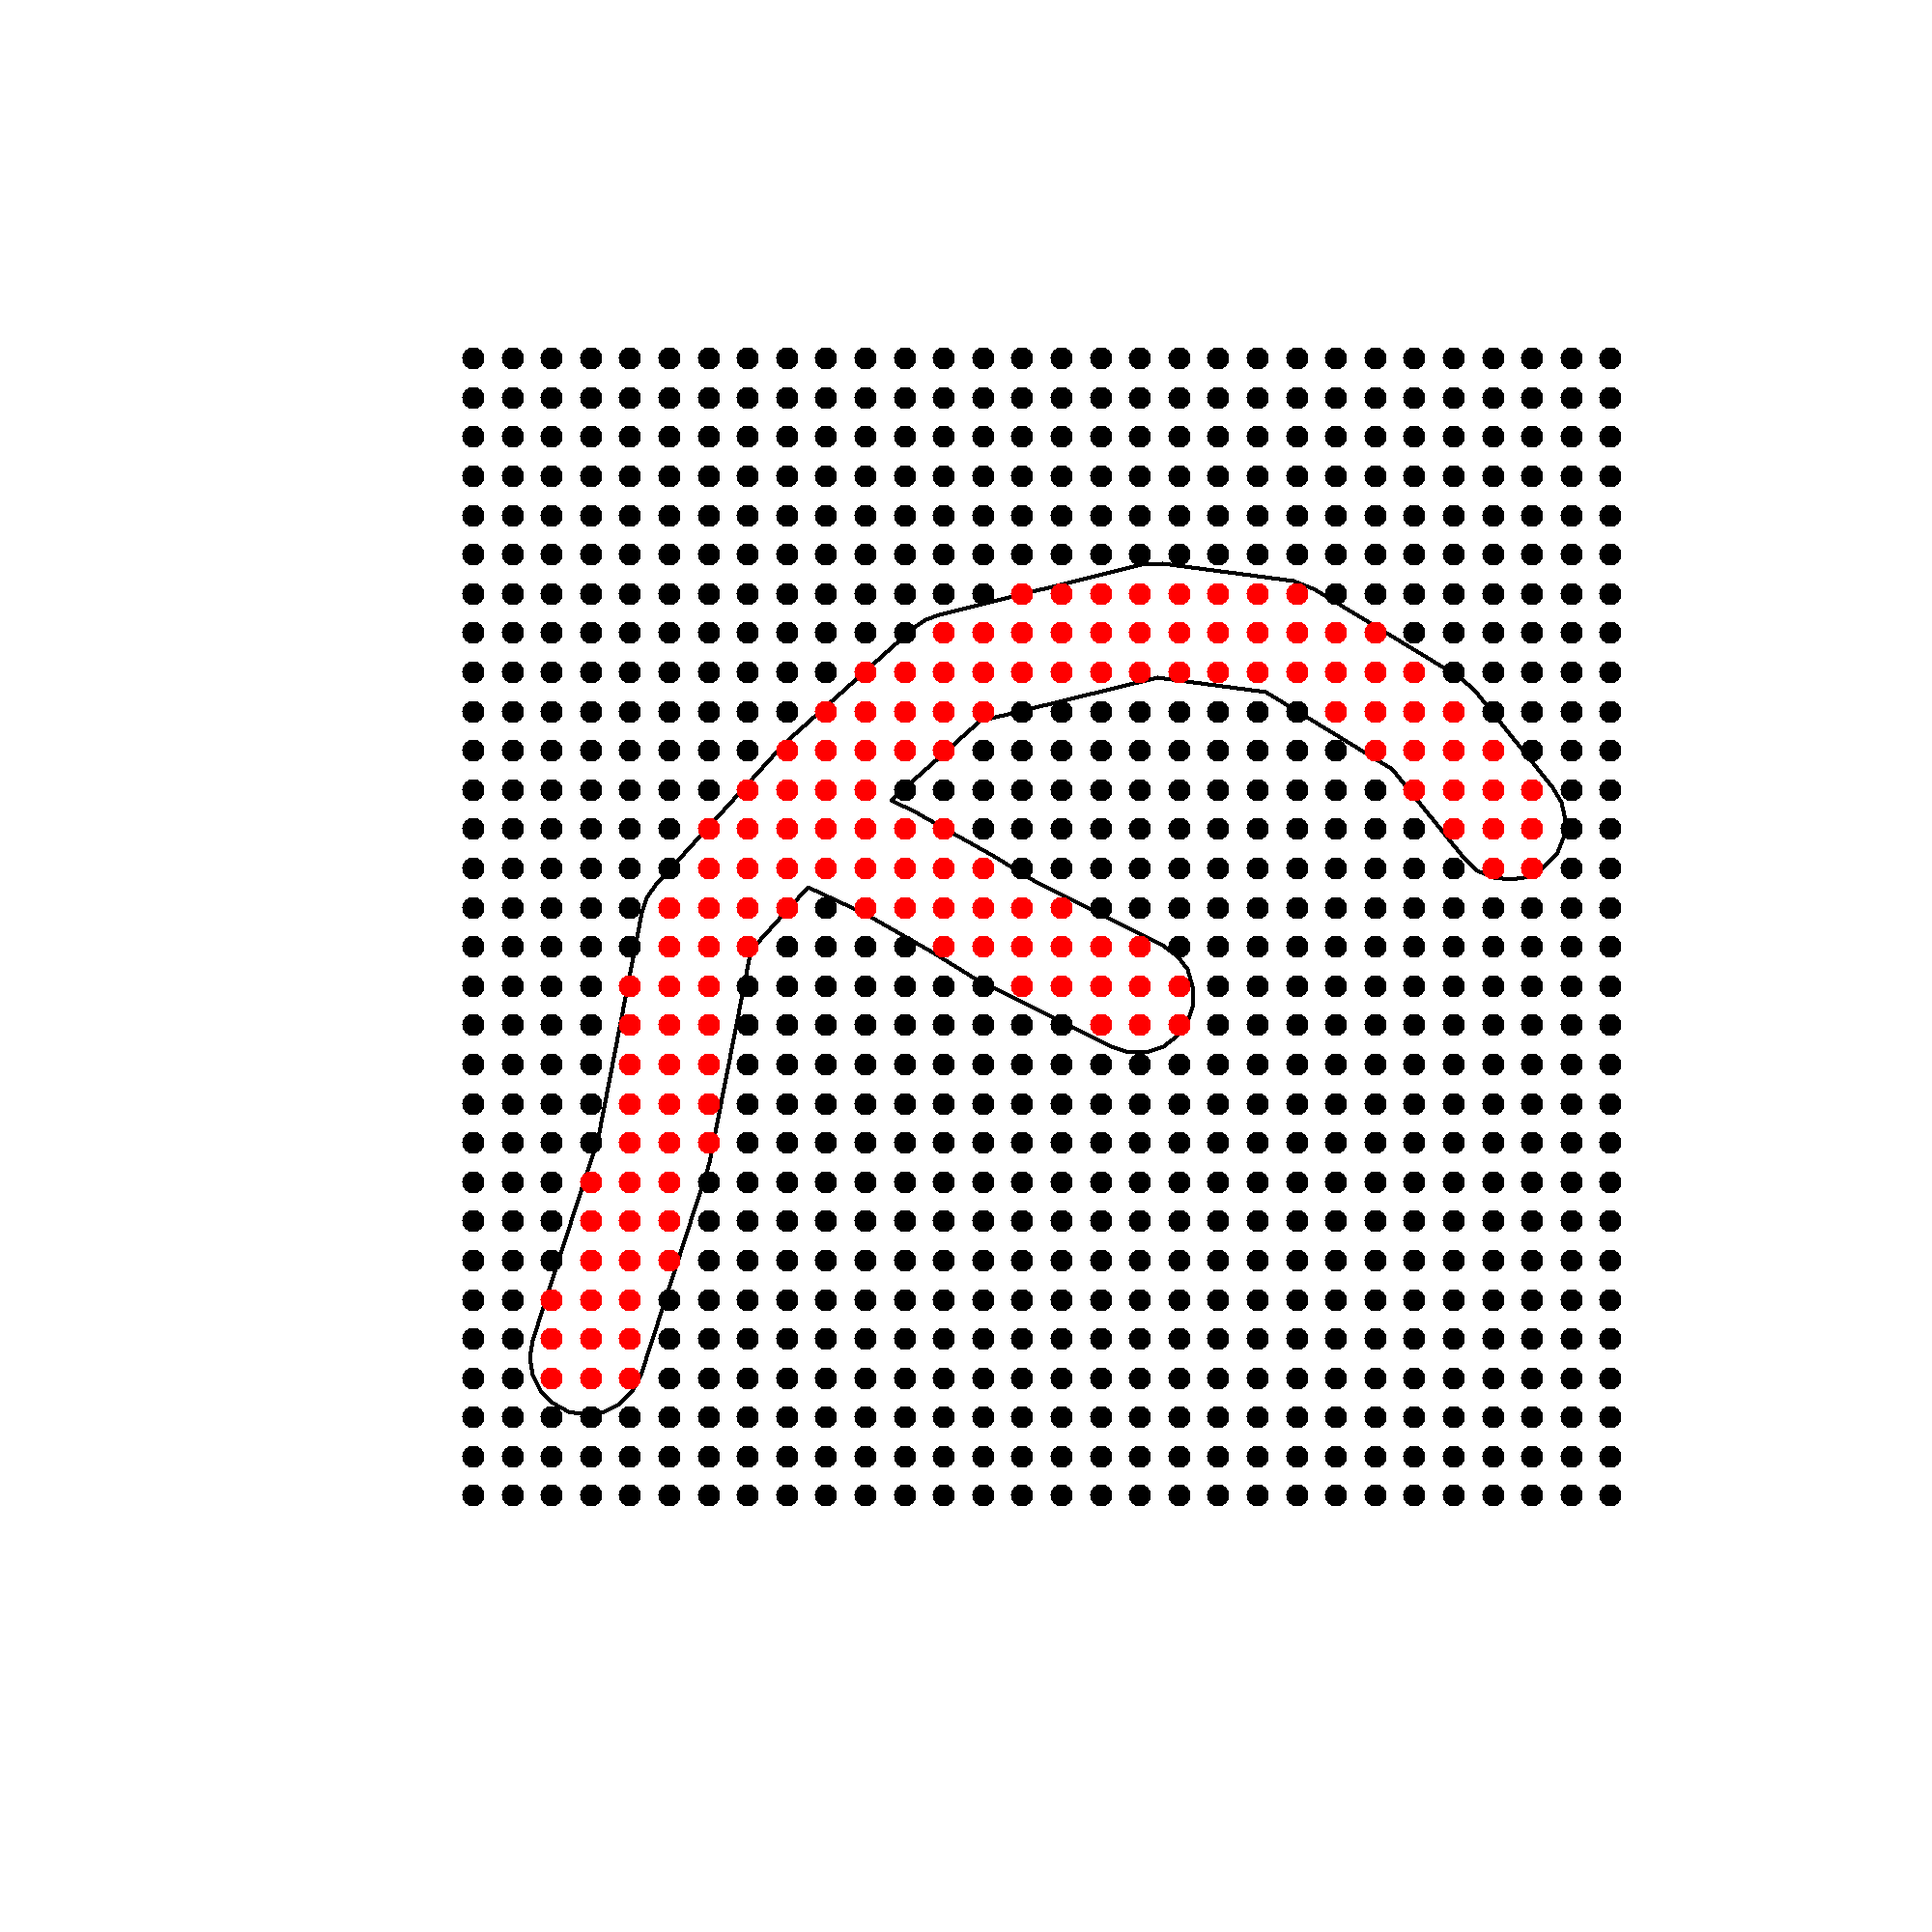
\includegraphics[height=3.25in,width=3.25in]{Ch10/figs/corridor}
\end{center}
\caption{A made-up corridor or reserve.}
\label{ecoldist.fig.corridor}
\end{figure}


We focus on devising a SCR model for this corridor system and we
imagine that animals will tend to severely avoid leaving the buffered
habitat zone. Therefore, we assign $\mbox{\tt cost}=1$ if a pixel is within the
buffer,
and $\mbox{\tt cost} = 10000$ if a pixel is outside of a
buffer. Therefore the cost to move to a neighboring pixel outside of
the buffered area is $5000.5$ compared to the cost of 1 to move to a
neighboring pixel inside the buffer. 

In this example, we're not going to estimate parameters of the cost
function. Therefore, in that case, we can compute the ecological
distance matrix one time and modify our likelihood code to accept the
distance matrix as input. We give that likelihood in the library
\mbox{\tt scrbook} as the function \mbox{\tt intlik3edv2}.
We note also that it provides a vector of 0's and 1's that
define any potential state-space restrictions. In the analysis of this
simulated data set, we define the state-space to be the buffered
corridor system. The help file for \mbox{\tt intlik3edv2} contains the
script that follows.

In this case we simulate N=200 guys in the corridor system and so we
restrict out state-space accordingly for purposes of fitting the
model. However we encourage the reader to refit the model without the
state-space restriction (for fitting the model only) and then
contemplate the result.  The code for doing all of this is as follows

{\small 
\begin{verbatim}
cost<-rep(NA,nrow(pts))
cost[in.pts==1]<-1      # low cost to move among pixels but not 0
cost[in.pts!=1]<-10000  # high cost 

library("raster")
r<-raster(nrows=40,ncols=40)
projection(r)<- "+proj=utm +zone=12 +datum=WGS84"
extent(r)<-c(0-delta/2,10+delta/2,0-delta/2,10+delta/2)
values(r)<-matrix(cost,40,40,byrow=FALSE)
par(mfrow=c(1,1))
plot(r)
points(pts,pch=20,cex=.4)

library("gdistance")
tr1<-transition(r,transitionFunction=function(x) 1/mean(x),directions=8)
tr1CorrC<-geoCorrection(tr1,type="c",multpl=FALSE,scl=FALSE)
costs1<-costDistance(tr1CorrC,pts)
outD<-as.matrix(costs1)
plot(pts,pch=".")
points(pts[in.pts==1,],pch=20,col="red")

library(``scrbook'')
traplocs<-traps$loc
trap.id<-traps$locid
ntraps<-nrow(traplocs)

set.seed(2013)
N<-200
S.possible<- (1:nrow(pts))[in.pts==1]
S.id<-sample(S.possible,N,replace=TRUE)
S<- pts[S.id,]

D<- outD[S.id,trap.id]
eD<- e2dist(S,traplocs)
Dtraps<-outD[trap.id,]

alpha0<- -1.5
sigma<- 1.5
beta<- 1/(2*sigma*sigma)
K<-10

probcap<-plogis(alpha0)*exp(-beta*D*D)
Y<-matrix(NA,nrow=N,ncol=ntraps)
for(i in 1:nrow(Y)){
 Y[i,]<-rbinom(ntraps,K,probcap[i,])
}
Y<-Y[apply(Y,1,sum)>0,]

frog1<-nlm(intlik3edv2,c(-2.5,2,log(4)),hessian=TRUE,y=Y,K=K,X=traplocs,
            S=pts,D=Dtraps,inpoly=in.pts)
frog2<-nlm(intlik3edv2,c(-2.5,2,log(4)),hessian=TRUE,y=Y,K=K,X=traplocs,
            S=pts,D=Deuclid,inpoly=in.pts)
\end{verbatim}
}

In the example that we ran abovve we compared the result for using
distance-within-the-corridor to normal Euclidean distance and the
results do not differ too much in this single instance. 



\section{A stream network}

Later we might add a 3rd prototype situation involving a stream network. 

We could use ``distance from stream'' to model effects of habitat
and corridors or whatever


\section{Summary and Outlook}


All published applications of SCR models to date have been based on models for the
encounter probability that are functions of the standard Euclidean
distance between individuals and traps. The obvious limitations are
that it is unaffected by landscape or habitat structure and implies
stationary, isotropic and symmetrical home ranges. These are standard
criticisms of the basic SCR model as universally applied in
practice. However, it is not a relevant criticism of the basic
conceptual formulation of SCR models, because, as we have
demonstrated, one can modify the Euclidean distance metric to
accommodate more realistic space usage considerations.  Following
\citet{royle_etal:2012ecol},
we demonstrated how to use 
minimum cost-weighted distance (i.e., ``least-cost
path'') between points, and where ``cost'' is characterized by one or
more spatially explicit covariates that are believed to influence
movement or space-usage of individuals. 

How animals use space and therefore how distance to a trap is
perceived by individuals is not something that can ever be known. We
can only ever conjure up models to describe this phenomenon and fit
those models to limited data on a sample of individuals during a
limited amount of time.  Here we have shown that there is hope to
estimate parameters, from capture-recapture data, that describe how
animals use space and thereby allow for irregular home range geometry
that is influenced by landscape structure.

Not surprisingly, our simulation study demonstrated
(Table 2) that the MLE of model parameters is
approximately unbiased in moderate sample sizes. Moreover, the effect
of ignoring ecological distance and using normal Euclidean distance in
the model for encounter probability, has the logical effect of causing
negative bias in estimates of $N$.  We expect this because the effect
is similar to failing to model heterogeneity. i.e., if we mis-specify
``model Mh'' \citep{otis_etal:1978} with ``Model M0''
\citep{otis_etal:1978} then we will expect to under-estimate $N$. So
the effect of mis-specifying the ecological distance metric with a
standard homogeneous Euclidean distance has the same effect. As a
practical matter, it stands to reason that many previous applications
of SCR models based on homogeneous distance metrics have under-stated
density of the focal population.

In our view, this bias is not really the most important reason to
consider models of ecological distance. Rather, inference about the
structure of ecological distance is fundamental to many problems in
applied and theoretical ecology related to modeling landscape
connectivity, corridor and reserve design, population viability
analysis, gene flow, and other phenomena.  Our new model allows
investigators to evaluate landscape factors that influence movement of
individuals over the landscape from non-invasively collected
capture-recapture data.  Therefore SCR models based on ecological
distance metrics might aid in corridor design and understanding other
aspects of space usage and movement in animal populations.

We adopted a standard approach to inference under our model based on
marginal likelihood \citep{borchers_efford:2008}. In principle,
Bayesian analysis does not pose any unique challenges for this new
class of models, except that computing the cost-weighted distance is
computationally intensive.  So, having to do this at each iteration of
an MCMC algorithm may be impractical using existing algorithms.  A
related issue is that the size of the raster slows things down. For
very large rasters, even likelihood analysis can be computationally
challenging and methods for efficient calculation of the ecological
distance given the raster covariate(s) and parameters might be needed.


Some additional extensions of the model may be of general interest.
We have used least-cost paths here to represent ecological distance
although other distance metrics could be used, including circuit
resistance distances \citep{mcrae:2006} which allows that animals can
move through multiple paths in the landscape.  Instead of
characterizing cost with explicit covariates it might be possible to
estimate the ``resistance surface'' as a latent field, much as
\citep{wikle:2003} did in the developing of models of species spread
based on a diffusion process. He defined the spatially-explicit rate
of diffusion, $\delta(x)$, as a Gaussian spatial process and it was
estimated from the data.




\begin{table}[h!]
\label{tab.results1}
{\small
\caption{Simulation results for estimating population size $N$ for a prescribed state-space with
$N=100$ or $N=200$ and various levels of replication ($K$) chosen to affect the observed sample
size of individuals (Tab. \ref{tab.samplesize}). For each simulated data set, the SCR model was fitted with
standard Euclidean distance (``euclid''), least-cost path assuming the
cost parameter $\theta_2$ is known (``lcp/known''), or allowing it to
be estimated by maximum likelihood (``lcp/est'').
The summary statistics of the
sampling distribution reported are the mean, standard deviation
(``SD'') and quantiles (0.025, 0.50, 0.975).
}
{\bf Systematic trend raster:} \\
\begin{tabular}{l|rrrrr|rrrrr}
         & \multicolumn{5}{c}{N=100   } & \multicolumn{5}{c}{N=200  }  \\
         &   mean &  SD  & 0.025 & 0.50 & 0.975  & mean  & SD   & 0.025 & 0.50  & 0.975 \\ \hline
K=3      &        &      &       &      &        &       &      &       &       &       \\
euclid   &   63.65& 12.62& 44.77 & 61.17&  90.98 & 126.68& 17.05&  98.93& 124.49& 168.26 \\
lcp/known&   99.28& 20.80& 68.83 & 97.55& 152.59 & 196.47& 27.39& 152.03& 192.96& 259.78\\
lcp/est  &  101.93& 21.68& 67.95 &101.56& 156.21 & 201.58& 28.14& 154.96& 200.15& 263.20\\
K=5      &        &      &       &      &        &       &      &       &       &        \\
euclid   &  64.60 & 7.11 & 51.52 & 63.86&  77.33 & 130.02& 10.25& 113.48& 128.96& 151.32\\
lcp/known&  95.96 &11.64 & 74.21 & 96.16& 117.65 & 193.04& 17.13& 166.84& 191.88& 226.16\\
lcp/est  &  98.94 &12.97 & 74.68 & 99.00& 123.88 & 198.80& 19.60& 166.87& 197.97& 239.46\\
K=10     &        &      &       &      &        &       &      &       &       &       \\
euclid   &  69.24 & 4.83 & 59.37 & 69.47&  79.18 & 139.83&  7.62& 125.65& 139.65& 154.82\\
lcp/known&  94.46 & 7.04 & 81.45 & 94.04& 108.83 & 190.47& 11.55& 170.49& 189.74& 213.19\\
lcp/est  &  97.53 & 8.18 & 82.02 & 97.62& 113.16 & 195.19& 13.28& 171.63& 194.58& 217.96\\ \hline
\end{tabular}
\\
{\bf Patchy "random" raster: } \\
\begin{tabular}{l|rrrrrrrrrr}
         & \multicolumn{5}{c}{N=100  } & \multicolumn{5}{c}{N=200   }  \\
         &   mean &  SD  & 0.025 & 0.50  & 0.975  & mean  & SD   & 0.025 & 0.50  & 0.975 \\ \hline
K=3      &        &      &       &       &        &       &      &       &       &       \\
euclid   &  78.68 & 18.12& 49.40 & 76.34 & 125.47 & 154.34& 33.74& 107.00& 146.34& 221.43\\
lcp/known& 109.09 & 27.52& 69.50 &104.86 & 183.72 & 207.18& 46.53& 143.31& 198.42& 315.89\\
lcp/est  & 110.96 & 28.65& 69.55 &106.98 & 181.84 & 208.77& 49.29& 141.68& 197.89& 325.77\\
K=5      &        &      &       &       &        &       &      &       &       &        \\
euclid   &  77.85 & 11.55& 59.17 & 77.44 & 101.14 & 153.39& 15.57& 129.31& 149.54& 185.38\\
lcp/known& 103.57 & 15.83& 78.15 &100.58 & 137.48 & 201.57& 21.25& 165.94& 199.95& 243.26\\
lcp/est  & 104.44 & 15.79& 78.38 &101.47 & 139.55 & 200.91& 20.78& 164.42& 200.47& 246.46\\
K=10     &        &      &       &       &        &       &      &       &       &       \\
euclid   &  78.01 & 5.26 & 68.00 & 77.96 & 87.81  & 156.27&  8.51& 142.17& 156.05& 174.55\\
lcp/known&  99.84 & 7.09 & 86.86 & 99.84 & 114.11 & 198.64& 11.04& 181.43& 197.62& 220.45\\
lcp/est  & 100.42 & 7.56 & 86.72 &100.34 & 115.47 & 198.45& 11.44& 180.06& 198.04& 219.52\\ \hline
\end{tabular}
}
\end{table}







\newpage







\begin{table}[ht]
{\small
\caption{Simulation results for estimating population size $N$ for a prescribed state-space with
$N=100$ or $N=200$ and various levels of replication ($K$) chosen to affect the observed sample
size of individuals. These results correspond to those of the
systematic landscape in Table 2 except with the traps
moved 0.5 units in from the boundary of the raster.
Each grouping of 3 rows (for a given value of $K$) summarizes the
performance of $\hat{N}$ under 3 distance models: (1) A model in which
Euclidean distance was used (``euclid''); (2) A model in which the
least-cost path distance was used, with the coefficient of the cost
function fixed (``lcp/known''); and (3) A model in which the
coefficient was estimated (``lcp/est''). The summary statistics of the
sampling distribution reported are the mean, standard deviation
(``SD'') and quantiles (0.025, 0.50, 0.975).
}
{\bf Systematic trend raster:} \\
\begin{tabular}{l|rrrrr|rrrrr}
         & \multicolumn{5}{c}{N=100   } & \multicolumn{5}{c}{N=200  }  \\
         &   mean &  SD  & 0.025 & 0.50 & 0.975  & mean  & SD   & 0.025 & 0.50  & 0.975 \\ \hline
K=3      &        &      &       &      &        &       &      &       &       &       \\
euclid   &   84.48& 20.42& 51.16 & 81.51& 140.62 &163.70 &24.55 &126.64 &157.67 &223.63 \\
lcp/known&  104.14& 25.49& 65.67 &101.50& 173.19 &200.16 &29.27 &158.65 &191.04 &268.78\\
lcp/est  &  105.90& 26.19& 65.95 &103.40& 182.30 &201.34 &29.54 &161.88 &192.36 &268.98\\
K=5      &        &      &       &      &        &       &      &       &       &       \\
euclid   & 81.21  &11.33 &61.35  &79.20 & 98.86  &163.27 &13.06 &140.21 &162.97 &185.94\\
lcp/known& 99.93  &12.86 &76.97  &99.75 &117.76  &199.80 &16.60 &170.25 &198.23 &227.66\\
lcp/est  & 100.84 &13.15 &79.96  &99.51 &119.08  &200.25 &16.53 &168.88 &199.29 &227.39\\
K=10     &        &      &       &      &        &       &      &       &       &       \\
euclid   &  80.10 & 7.81 &66.45  &79.14 &93.33   &158.40 & 9.25 &142.74 &157.86 &173.18\\
lcp/known& 100.07 & 9.50 &82.99  &100.33&114.81  &197.62 &12.58 &171.95 &199.21 &217.19\\
lcp/est  & 100.10 & 9.88 &82.31  &100.91&116.27  &197.52 &13.03 &169.49 &200.68 &217.82\\ \hline
\end{tabular}
}
\label{tab.results3}
\end{table}






















%\chapter{Ecological Distance Models in Spatial Capture-Recapture}
%\label{chapt.ecoldist}

\chapter{
Modeling Spatial Variation in Density
}
\markboth{Spatial Variation in Density}{}
\label{chapt.state-space}

\vspace{0.3cm}

Underlying every spatial capture-recapture models is a point process
that describes the number and distribution of animal activity
centers within the state-space ($\cal{S}$).
%, which is
%typically a two-dimensional polygon defining the study area.
A spatial point process is characterized by %$\mathcal{S}$ and by
an intensity parameter defined at each location in $\mathcal{S}$; and
in the case of SCR models, this intensity parameter is population
density. If the intensity is constant, density is constant throughout
$\mathcal{S}$ and the point process is said to be homogeneous.
Thus far we have focused our attention on homogeneous %binomial
point processes whose realized values are the locations of the $N$
activity centers within the state-space. When a Poisson prior is
placed on $N$, we have a homogeneous Poisson point process, which
is referred to as a model of ``complete spatial randomness.''
%because the point process intensity is constant
%and the activity centers do not interact with one another.
A similar model, that we often use in conjunction with data
augmentation and MCMC, places a binomial prior on $N$. This is also a
model of spatial randomness, and in this chapter we will compare and
contrast the two.

The spatial randomness assumption is often viewed as restrictive
because ecological processes such as
territoriality and habitat selection can result in non-uniform
distributions of organisms. We have argued, however, that this
assumption is less restrictive than may be recognized because a
homogeneous point process actually allows for infinite
possible ``point patterns'', or realized configurations of activity
centers. Furthermore, given enough data,
the uniform prior will have very little influence on the estimated
locations of activity centers. Nonetheless, a homogeneous point
process does not allow one to model population density using
covariates, which is an important objective in much ecological research.
For example, even when assuming a homogeneous point process model for
the activity centers, an estimated density surface may strongly
suggest that individuals are more abundant in one habitat than
another; however, such results do not provide the basis for formally testing
hypotheses about spatial variation in density, and they could not be
used to make predictions about habitat-specific abundance in other
regions. A more direct approach is to replace the homogeneous model
with an inhomogeneous model in which the point process intensity
is allowed to vary spatially.

In this chapter, we cover methods % we present a method
for fitting inhomogeneous Poisson and binomial
spatial point process models by treating the intensity parameter as a
function of covariates, in much the same way as is done in generalized linear
models. The covariates we consider differ
from those covered in previous chapters, which were typically
attributes of the animal (e.g. sex or age) or the trap (e.g. baited or
not) and were used to model movement or encounter
rate. In contrast, here we wish to model covariates that are defined
at all points in $\cal S$, which we will refer to as
state-space covariates or density covariates. These may
include continuous covariates such as elevation, or discrete
covariates such as habitat type. Such covariates are often formatted
as raster images with a prescribed resolution and extent.

Inhomogeneous Poisson point process models were discussed in the original
formulation of SCR models by \citet{efford:2004} and were described in
more detail by \citet{borchers_efford:2008}. We will show that an
inhomogeneous binomial point process is quite similar to the Poisson
model, but is more easily implemented in MCMC algorithms. To do so, we
will define the data augmentation parameter $\psi$ in terms of the point
process intensity function, and we will replace the uniform prior on the
activity centers with a prior that is also derived from the intensity
function. Development of this prior, which does not have a
standard form, is a central component of this chapter. First we
begin with a review of homogeneous point process models.


\section{Homogeneous point process revisited}

The homogeneous Poisson point process is \textit{the} model of complete
spatial randomness and is often used in ecology as a null model
to test for departures from randomness
\citep{cressie:1992, diggle:2003, illian_etal:2008}.
%Given its central role in spatial ecology, it is helpful to describe it briefly and
%compare it with the binomial model that we use in when conducting
%Bayesian analysis of SCR models.
The Poisson model asserts that the number of points in $\mathcal{S}$ is
Poisson distributed: $N \sim \text{Poisson}(\mu|\mathcal{S}|)$ where $\mu>0$ is
the intensity parameter and $|\mathcal{S}|$ is the area of the
state-space. The intensity parameter $\mu$
is the density of points, and thus multiplying the intensity by the area
of some region yields the expected number of points in that region.
As with all homogeneous point process models, the $N$ points are
distributed uniformly, which implies that they do not interact with each other in
any way---for example, they neither attract nor repel one another.

Unlike the Poisson point process, the
binomial point process assumes that $N$ is fixed, not random.
%In other words, the binomial point process conditions on $N$,
The distinction is illustrated by this simple \R~code that generates
realizations from Poisson and binomial point processes in the unit
square ($\mathcal{S} = [0,1]\times[0,1]$):

\begin{samepage}
\begin{verbatim}
Area <- 1                          # Area of unit square
muP <- 4                           # intensity
nP <- rpois(1, muP*Area)           # number of points: random
PPP <- cbind(runif(nP), runif(nP)) # Poisson point pattern

nB <- 4                            # number of points: fixed
muB <- nB/Area                     # intensity
BPP <- cbind(runif(nB), runif(nB)) # binomial point pattern
\end{verbatim}
\end{samepage}

{\flushleft Both of these models are homogeneous because the intensity parameter
is constant ($\mu=4$ in both cases) and the $N$ points do not interact
with each other. This results from the fact that the locations of the
points follow a uniform distribution on the plane. The key distinction
is that $N$ is random in the former and fixed in the latter.}

Another difference between the Poisson and binomial models is that if the
state-space is divided into $K$ disjunct regions, the number of points in each
region $n(B_k): k=1,\dots,K$; are independent and identically
distributed (i.i.d.) under the Poisson model but not under the
binomial model. In the Poisson case,
the counts are simply distributed as $n(B_k) \sim
\text{Poisson}(\mu|B_k|)$, where $|B_k|$ is the area of the region
$B_k$. For the binomial case, $n(B_k) \sim
\text{Binomial}(N, \pi(B_k))$ where $\pi(B_k)$ is the proportion of
the state-space in $B_k$; however, these counts are not
i.i.d. because the number of points in one region is informative
about the number of points in another region. For example, if
$N=10$, which would be known for a binomial point process, and if we
know that there are 7 points outside the region $B_1$,
then we can say with certainty that $B_1 = 10 - 7 = 3$.

Fig.~\ref{state-space.fig.homo} is meant to further illustrate the characteristics
of the binomial model. The left panel shows a point pattern
realized from a
homogeneous binomial point process with $N=50$. The right panel shows
the same realization, except that the state-space has been discretized
into 25 equally-sized disjunct regions, or pixels, and the counts in each pixel
are shown. Since the pixels are the same
size, $\pi(B_k) = 1/25$, the expected number of point in each
pixel is 2: $\mathbb{E}(n(B_k)) = N\pi(B_k) = 50/25$, which
happens to be the empirical mean in this instance. However, as
previously stated, these counts are not
independent realizations from a binomial distribution since $\sum_k
n(B_k) = N$. Rather, the model for the entire vector is multinomial:
$\{n(B_1), n(B_2), \dots, n(B_k)\} \sim \mbox{Multinomial}(N, \{p(B_1), p(B_2), \dots,
p(B_K) \})$ \citep{illian_etal:2008}. If you need a refresher on the
multinomial distribution, refer to Sec.~\ref{modeling.sec.multinom}, and
consider the following \R~code, which generates counts such as those
seen in Fig.~\ref{state-space.fig.homo}:
\begin{verbatim}
n.Bk <- rmultinom(1, size=50, prob=rep(1/25, 25))
matrix(n.Bk, 5, 5)
\end{verbatim}

\begin{figure}%[ht!]
\centering
%\includegraphics[width=5in,height=2.5in]{Ch11/figs/homoPlots}
\includegraphics[width=\textwidth]{Ch11/figs/homoPlots}
\label{state-space.fig.homo}
\caption{Homogeneous binomial point process with $N$=50 points
  represented in continuous and discrete space.}
\end{figure}

The dependence among counts has virtually
no practical consequence when the number of pixels is large. For
example, if there are 100 pixels, the number of points in one pixels
carries very little information about the expected number of points in another
pixel. However, if there are only 2 pixels, then clearly the number of
points in one pixel allows one to determine how many points will occur in the
remaining pixel.

The discrete representation of space shown in
Fig.~\ref{state-space.fig.homo} is not only helpful for understanding
the properties of a point process, it is also of practical importance
when fitting SCR models because spatial covariates are almost always
represented as rasters, i.e. grids with predetermined extent and
resolution. In such cases, the definition of the prior for
the point locations can be changed from the probability that a point
occurs at some location in space to the probability that it occurs in
some pixel of the raster. As we will explain in
Sec.~\ref{modeling.sec.discrete}, this typically involves changing the
prior from a uniform distribution to a multinomial or categorical
distribution.

Up to this point in this chapter we have sketched out the basic characteristics
of homogeneous Poisson and binomial point process models. Now we need
to speak more specifically about their relevance to SCR models before we move on
to the inhomogeneous models. %Much of this has already been in previous
%chapters, but we feel it is important enough to review here.
In a SCR model with a homogeneous point process, the intensity
parameter $\mu$ is interpreted as population density, and $N$ is
interpreted as population size\footnote{Strictly speaking, $N$ is the
  number of activity centers in $\mathcal{S}$}. These interpretations
are true regardless of whether we consider the
Poisson model or the binomial model, but since $N$ is always unknown, one
might wonder why we are discussing the binomial model at all. %Indeed,
%the binomial model was not mentioned by \citet{efford:2004} or
%\citet{borchers_efford:2008}. Instead, they focused exclusively on the
%Poisson model and estimation of $\mu$, with $N$ being regarded as a
%derived parameter.

In our work, we typically adopt the binomial model simply
because it is easy to implement using MCMC and data
augmentation. And while $N$ is truly unknown, we use an upper bound $M$
which is fixed. Thus, the standard point process we use Bayesian in
analyses can be
regarded in two ways. First, it is a binomial point process with $M$
points. Second, in terms of $N$, it is a thinned binomial point
process, where $\psi$ is the thinning parameter.
\hl{XXXX Is this thinned point process also binomial, even though N is
  no longer fixed? XXXX}.
With this in mind,
the only real difference between the Poisson and binomial models, as
implemented in SCR contexts, is that in the former, we have
$N \sim \text{Poisson}(\mu|\mathcal{S})$, and in the latter we have
$N \sim \text{Binomial}(M, \psi)$. In other words, we just have a
different prior on $N$, and when using MCMC, the binomial prior is
much more convenient because it fixes the size of the parameter space
and makes it easy to extend the model in each of the ways discussed in
this book. It is also worth remembering that the Poisson
distribution is the limit of the binomial distribution when $M$ is
very high and $\psi$ is very low (Chapt.~\ref{chapt.modeling}), and
thus the two models are much more similar than may appear.

You might have noticed that the intensity parameter $\mu$ was not shown for the
binomial prior $N \sim \text{Binomial}(M, \psi)$. Instead, we see the
data augmentation parameter $\psi$, which has been used throughout
this book, but without much mention of the point process
intensity. What then is the relationship between $\psi$ and $\mu$?
As first discussed in Chapt.\ref{chapt.scr0}, under data augmentation,
the expected value of $N$ is $\mathbb{E}[N] = M\psi$. But, from this
chapter, we also know that the
expected value of $N$ can be written in terms of $\mu$ as
$\mathbb{E}[N] = \mu|\mathcal{S}|$. Therefore,
$\psi = \mu|\mathcal{S}| / M$ and hence we can directly estimate $\mu$
rather than $\psi$ if we so desire---and we will so desire in the next
section where the objective is to model $\mu$ as a function of
spatially-referenced covariates. First, as an exercise, execute the
following \R~commands to familiarize yourself with some of the
concepts we just covered:
\begin{small}
\begin{verbatim}
Area <- 1                  # Area of state-space
M <- 100                   # Data augmentation size
mu <- 10                   # Intensity (points per area)
psi <- (mu*Area)/M         # Data augmentation parameter (thinning rate)
N <- rbinom(M, 1, psi)     # Realized value of N under binomial prior
cbind(runif(N), runif(N))  # Point pattern from thinned binomial model
\end{verbatim}
\end{small}
%This code illustrates the fact that $\psi$ can be expressed as a
%function of the point process intensity $\mu$. Thus each and every
%MCMC algorithm used in this book could have been parameterized in
%terms of $\mu$ rather than $\psi$. However, you might have noticed
%that the above code does not include the indicator variables

\begin{comment}
  We conclude this section by pointing out
  Table\ref{state-space.tab.pvb}, which highlights the differences of
  the homogeneous Poisson and binomial point process models as they
  relate to SCR. % XXXX Need to fill in this table XXXX

\begin{table}
  \centering
  \caption{Characteristics of homogeneous point
    processes. Table~\ref{state-space.tab.hetero} describes the
    inhomogeneous models.}
  \begin{tabular}{lccc}
    \hline
    & Prior & $\mathbb{E}[N]$    & $\mu$   \\
    \hline
    Poisson  & $N \sim \text{Poisson}(\mu|\mathcal{S}|)$   &  &  \\
    Binomial & $N \sim \text{Binomial}(M, $   & $M\psi = $   &  &  \\
    \hline
  \end{tabular}
  \label{state-space.tab.homo}
\end{table}
\end{comment}


\section{Inhomogeneous point processes}

The principal difference between homogeneous and inhomogeneous point
processes is that the intensity parameter $\mu$ is allowed to vary spatially
in the latter. Thus, rather than $\mu$ being a fixed constant,
it is now a function defined at each point $\mathbf{s} \in
\mathcal{S}$. A vast number of options exist for modeling spatial
variation in the intensity of a point process
\citep{cox:1955,stoyan_penttinen:2000,illian_etal:2008}, but here we
focus on modeling $\mu$ as a function of
spatially-referenced covariates and a vector of regression
coefficients $\bm \beta$; a function we will denote $\mu(\mathbf{s},
\bm{\beta})$. To be clear, $\mu(\mathbf{s}, \bm{\beta})$, is a
function that returns the expected density of activity centers at
location $\bf s$, given the covariate values at $\bf s$.  Since the
intensity must be positive, and because the natural logarithm is the
canonical link function of the Poisson generalized linear model
\citep{mccullagh_nelder:1989}, it is natural to consider the following model:
\begin{equation}
  \log(\mu(\mathbf{s}, {\bm \beta})) = \beta_0 + \sum_{v=1}^V \beta_v z_v(\mathbf{s})%, \quad  \mathbf{s} \in \cal{S}
  \label{state-space.eq.loglin}
\end{equation}
which says that there are $V$ covariates and $\beta_v$ is the
regression coefficient for covariate $z_v(\mathbf{s})$. This
covariate, $z_v(\mathbf{s})$, could be any variable defined at all points
in the state-space, such as habitat type or elevation.
Eq.~\ref{state-space.eq.loglin} should look familiar because it is the
standard linear predictor used in Poisson regression. As with other
GLMs, one could consider alternative link functions.

Recall from the previous section that for a homogeneous point process,
the expected number of points in the state-space was simply the
intensity parameter multiplied by area: $\mathbb{E}[N] =
\mu|\mathcal{S}|$. But now that we are regarding the intensity as a
function, rather than a scalar, this equation is not very useful. So
what is $\mathbb{E}[N]$ for an inhomogeneous point process?
%And why do
%we care? Well, hopefully you remember that the reason we need a
%the reason we care is that we want a model that
Contemplating a discrete state-space is useful for figuring this
out. Imagine that the state-space is represented as a raster with many
tiny pixels. In this case, we will associate
$\bf s$ with pixel ID, i.e. $\bf s$ just references some pixel with
$V$ covariates values associated with it. The expected number of
individuals in this pixel, say $\mathbb{E}[n(\mathbf{s})]$, can intuitively be
found by evaluating the intensity function
(Eq.~\ref{state-space.eq.loglin}) and multiplying it by the area of
the pixel. In other words, we compute the expected number of
individuals in a pixel by multiplying the expected value of density
for that pixel by the area of the pixel. If we do this for each pixel in the state-space, then
summing up these values gives us what we are after, the expected value
of $N$. Specifically,
$\mathbb{E}[N] = \sum_{\mathbf{s} \in \mathcal{S}}
\mathbb{E}[n(\mathbf{s})]$.
As the area of the pixels approaches zero, such that we move from discrete
space back to continuous space, the summation must be replaced
with an integration of the form:
\begin{equation}
\mathbb{E}[N] = \int_{\mathcal{S}} \mu(\mathbf{s}, {\bm \beta}) \mathrm{d}\mathbf{s}.
\label{state-space.eq.EN}
\end{equation}
Together, Eqs.~\ref{state-space.eq.loglin} and \ref{state-space.eq.EN}
describe a model for spatial variation in density as well as
population size. The key task in fitting such inhomogeneous point
process models is to estimate the $\bm \beta$
parameters.

We have now described an approach for modeling the point process
intensity, yet in order to define the likelihood or to develop an MCMC
algorithm for the inhomogeneous model, we need to specify the prior
distribution for the activity centers. Recall that under the
homogeneous point process, the prior was
$\mathbf{s}_i \sim \text{Uniform}(\mathcal{S})$, for $i=1,\dots,N$, or
equivalently:
\begin{equation}
  \label{state-space.eq.uprior}
  [\mathbf{s}_i] = 1/|\mathcal{S}|
\end{equation}
where once again $|\mathcal{S}|$ denotes the area of the
state-space. This simply indicates that an activity center is equally
likely to occur at any location in the state-space.
However, if animals exhibit habitat selection or simply
occur in one region more often than another, it would be preferable to
replace this prior with one describing the spatial variation in
density. Clearly this prior should be determined in some way by the
spatially-varying intensity function $\mu(s, \bm{\beta})$.
%The key to determining this prior is to recall that
Since
the integral of a probability density function (pdf) must be unity,
we can convert $\mu(\mathbf{s}, \bm{\beta})$ into a pdf by dividing it by a
normalizing constant. In this case, the normalizing constant is found by integrating
$\mu(s, \bm{\beta})$ over the entire state-space.
The probability density function of the new prior is therefore:
\begin{equation}
[\mathbf{s}_i | \bm{\beta}] = \frac{\mu(\mathbf{s}_i, \bm{\beta})}{\int_{\mathcal{S}} \mu(\mathbf{s}, \bm{\beta})\, \mathrm{d}\mathbf{s}}
\label{state-space.eq.pdf.hetero}
\end{equation}
Substituting the uniform prior with this new distribution
allows us to fit inhomogeneous binomial point process
models to spatial capture-recapture data.
%We can also use this
%distribution to obtain the expected number of individuals in any given
%region $B \in \mathcal{S}$. Specifically, the proportion of $N$ expected to occur in
%$B$ is $\pi(B) = \int_B [\mathbf{s} | \bm{\beta}]\, \mathrm{d}x$. These are
%also the conditional-on-$N$ multinomial cell probabilities if the regions are
%disjoint and compose the entire state-space. We provide an example in
%the next section, and in Fig.\ref{state-space.fig.hetero}.

As a practical matter, note that the integral in the
denominator of Eq.~\ref{state-space.eq.pdf.hetero} is evaluated over
space, and since we always regard space as two-dimensional (the
state-space is planar), this is a two-dimensional integral that can
be approximated using the methods discussed in
Chapter~\ref{chapt.poisson-mn}, which include
Monte Carlo integration and Gaussian quadrature. Alternatively, if
our state-space covariates are in raster format, i.e. they are
in discrete space, the integral can be replaced with a summation over
all the pixels in the raster,
\begin{equation}
[\mathbf{s}_i | \bm{\beta}] = \frac{\mu(\mathbf{s}_i, \bm{\beta})}{\sum_{\mathbf{s} \in \mathcal{S}} \mu(\mathbf{s}, \bm{\beta})}
\label{state-space.eq.pdf.hetero.d}
\end{equation}
where $\bf s$ is now defined as ``pixel ID'' rather than a point in space.

Although the discrete space approach is standard practice, it is
technically unjustified because covariate values must be known for all
points in space. This same problem is present anytime that we have a
sample of the spatial covariates, rather than a function defining
their value for all points in space. In such cases, it may be necessary to
interpolate the values of the covariates for points in space where
they were not measured. One option would be to use a Kriging
interpolator, as demonstrated by \citet{rathbun:1996}. Another option
is to sample the spatial covariates using probabilistic sampling
methods, which allow for design-based estimators of their values for
the entire study area \citep{rathbun_etal:2007}. Either option could
be implemented within maximum likelihood or MCMC estimation methods;
however,
%even though such approaches are technically necessary,
we do not demonstrate them here
because it seems likely that they will be inconsequential in most
cases where the raster data are of high resolution, such that the loss
of information is negligible when going from continuous space to
discrete space. Furthermore, the validity of this assertion, and the
level of resolution required to adequately approximate continuous
space can often be assessed by checking the consistency of the
parameter estimates among varying levels of resolution, as was
demonstrated in Chapt.~\ref{chapt-scr0}.

We now have all the tools needed to fit inhomogeneous point process
models. Likelihood-based inference for inhomogeneous Poisson point
process models was described by \citet{borchers_efford:2008} and
reviewed in Chapt.~\ref{chapt.mle}. Another example is demonstrated in
the next section, but first we focus on the binomial
model that we favor when conducting Bayesian inference. In the
previous section we noted that the data augmentation parameter $\psi$
can be expressed in terms of the intensity parameter $\mu$. The same
is true for inhomogeneous models. Specifically, rather than
$\mathbb{E}[N] = \psi M$ as before, we use the expected value of $N$ shown
in Eq.~\ref{state-space.eq.EN} which results in
\begin{equation}
\psi = \frac{\int_{\mathcal{S}} \mu(\mathbf{s},
  \bm{\beta}) \, \mathrm{d}\mathbf{s}}{M}
\label{state-space.eq.psimu}
\end{equation}
Note that the data augmentation limit $M$ must be high enough so that
it is greater than the numerator---i.e. the expected value
of $N$ must be less than $M$.

If we refer to the distribution $[\mathbf{s}_i | \bm{\beta}]$ as
``IPP'', we can write a hierarchical description of a SCR model with a
Binomial encounter process and a half-normal, or Gaussian, detection function as
\begin{gather*}
w_i \sim \mbox{Bernoulli}(\psi) \\
{\bf s_i} \sim \mbox{IPP}(\mu(\mathbf{s},\beta)) \\
p_{ij} = p_0 \exp(-\|{\bf s_i} - {\bf x_{j}}\|^2/(2\sigma^2)) \\
y_{ij} \sim \mbox{Binomial}(K, p_{ij} w_i)
\end{gather*}
The new prior for $\mathbf{s}_i$ and Eq.~\ref{state-space.eq.psimu}
%use of $\mbox{IPP}(\mu(s, \beta))$ instead of
%$\mbox{Uniform}(\cal{S})$ is the
are the key differences between homogeneous an inhomogeneous
models.

\begin{comment}
The IPP for the activity centers
results in another IPP for the observation process, $\lambda(s)$, the
expected number of captures for a trap
at point. As was true for the homogeneous model, this
intensity function is a product of the point process intensity
and the encounter rate function, $\lambda(s) = \mu(s, {\bm \beta})
\lambda_{ij}$.
\end{comment}

In the next sections we walk through a few examples, building up from
the simplest case where we actually observe the activity centers as
though they were data. In the second example, we fit our new model to simulated
data in which density is a function of a single continuous
covariate. To build upon the developments in the previous chapter, we
further consider the plausible case where a state-space covariate is also a
covariate of ecological distance. A small simulation study indicates
that both effects can be estimated. A fourth example shows an analysis in discrete space using
both \secr~\citep{efford:2011} and \jags~\citep{plummer:2003}. In the
fifth and final example, we model the intensity of
activity centers for a real dataset collected on jaguars
(\emph{Panthera onca}) in Argentina.

\section{Observed Point Processes}

In SCR models, the points (activity centers) are not directly
observed, but in other contexts they are. Examples include the
locations of disease outbreaks, the locations of trees in a forest, or
the locations of radio-tracked animals. In such cases, it is
straightforward to fit inhomogeneous point process models and estimate the
%Indeed Eq.~\ref{eq.pdf.ipp}
%has been used extensively in the radio-telemetry literature to model
%so-called ``resource selection functions''
%\citep{manly_etal:2002,lele_keim:2006}. When the point locations are
%directly observed, estimating
the parameters $\bm \beta$ from Eq.~\ref{state-space.eq.loglin}, as we
will do in the following example. % is
%straight-forward as demonstrated in the following example.
%This example also illustrates the fundamental process that we will
%later embed in our MCMC algorithm used to fit SCR models that include
%an inhomogeneous point process.

Suppose we knew the locations of $N$ animal activity
centers, perhaps as the result of an extensive telemetry study. %To
%estimate the intensity surface $\mu(\mathbf{s}, \bm{\beta})$ underlying these
%points, we need to derive the likelihood for the data under this
%model.
If we assume $N$ is Poisson distributed and the points are
mutually independent of one another, we can fit the
inhomogeneous Poisson point process model whose likelihood is
the product of $N$ densities given by
Eq.~\ref{state-space.eq.pdf.hetero} \citep[pg. 104]{diggle:2003}. The
log-likelihood is thus:
\[
\ell({\bm \beta} | \{{\bf s}_i\}) = \sum_{i=1}^N
\log(\mu(\mathbf{s}_i, \bm{\beta})) - \int_{\mathcal{S}} \mu(\mathbf{s}, \bm{\beta}) \, \mathrm{d} \mathbf{s} .
\]
Having defined the likelihood we could choose a prior distribution for
$\bm \beta$ and obtain the posterior distribution %of $\bm \beta$
using Bayesian methods, or we can find the maximum likelihood
estimates (MLEs) using standard numerical methods as is demonstrated
below.

First, we simulate some data under the model $\mu(\mathbf{s},
\bm{\beta}) = \beta_0 + \beta_1\mathrm{ELEV}(\mathbf{s})$, where
$\mathrm{ELEV}(\mathbf{s})$ is a spatial covariate, say
elevation, and $\beta_0=5$ and $\beta_1=2$. It is worth emphasizing
that a spatial covariate must be defined at any location $\bf s$,
which is demonstrated by the following \R~code.
%\begin{samepage}
  \begin{small}
\begin{verbatim}
elev.fn <- function(s) {          # spatial covriate
    s <- matrix(s, ncol=2)        # Force s to be a matrix
    (s[,1] + s[,2] - 100) / 40.8  # Returns (standardized) "elevation"
}
# intensity function
mu <- function(s, beta0, beta1) exp(beta0 + beta1*elev.fn(s=s))
beta0 <- -6 # intercept of intensity function
beta1 <- 1  # effect of elevation on intensity
# Next line computes integral
EN <- cuhre(2, 1, mu, beta0=beta0, beta1=beta1,
            lower=c(0,0), upper=c(100,100))$value
\end{verbatim}
  \end{small}
%\end{samepage}
The function \texttt{elev.fn} returns the value of elevation at any
location, which can be either a two-dimensional vector for the
coordinates of a single point, or it can be matrix with two columns
for a collection of points. The standardization bit is not necessary,
but helps with the model fitting below. The next lines of the code define the
intensity function $\mu(\mathbf{s}, \bm{\beta})$ in terms of elevation
and the regression coefficients. The last line uses the \verb+cuhre+ function in
the {\tt R2Cuba} package \citep{hahn_etal:2011} to compute the
expected value of $N$ in a $[0,100]\times[0,100]$ square state-space, which is the
two-dimensional integral of Eq.~\ref{state-space.eq.pdf.hetero}. This
integral could also be computed using a fine grid of points as we have done in previous
chapters, but it is useful to gain familiarity with more efficient
integration functions in \R.

The \R~code above demonstrates how to obtain the expected value
of $N$ given a spatial covariate and the coefficients defining the
intensity function. Now we need to generate a realized value of $N$
and distribute the $N$ points in proportion to the intensity
function. This is not as simple as it was to simulate data from a homogeneous point process
because the points are no longer uniformly distributed within the
state-space. Instead one must resort to methods such as rejection sampling, which involves
simulating data from a standard distribution and then accepting or
rejecting each point using probabilities defined by the distribution
of interest. For more information, readers should consult an
accessible text such as \citet{robert_casella:2010}. In our example, we
simulate from a uniform distribution and then accept or reject using
the (scaled) probability density function
$[\mathbf{s}_i | \bm{\beta}]$
(Eq.~\ref{state-space.eq.pdf.hetero}). The following \R~commands
demonstrate the use of
rejection sampling to simulate an inhomogeneous point process for the
elevation covariate depicted in
Fig.~\ref{state-space.fig.hetero}.
%\begin{samepage}
  \begin{small}
\begin{verbatim}
set.seed(31025)
N <- rpois(1, EN)     # Realized N
s <- matrix(NA, N, 2) # This matrix will hold the coordinates
elev.min <- elev.fn(c(0,0))
elev.max <- elev.fn(c(100, 100))
Q <- max(c(exp(beta0 + beta1*elev.min),  # max of intensity function
           exp(beta0 + beta1*elev.max)))
counter <- 1
while(counter <= N) { # begin rejection sampling
  x.c <- runif(1, 0, 100); y.c <- runif(1, 0, 100)
  s.cand <- c(x.c,y.c) # proposed activity center
  pr <- mu(s.cand, beta0, beta1)
  if(runif(1) < pr/Q) { # Typically rejected if pr is low
    s[counter,] <- s.cand
    counter <- counter+1
    }
  }
\end{verbatim}
  \end{small}
%\end{samepage}
Similar methods are also
implemented in the \R~package \texttt{spatstat} \citep{baddeley_turner:2005}.
\begin{figure}%[ht]
\centering
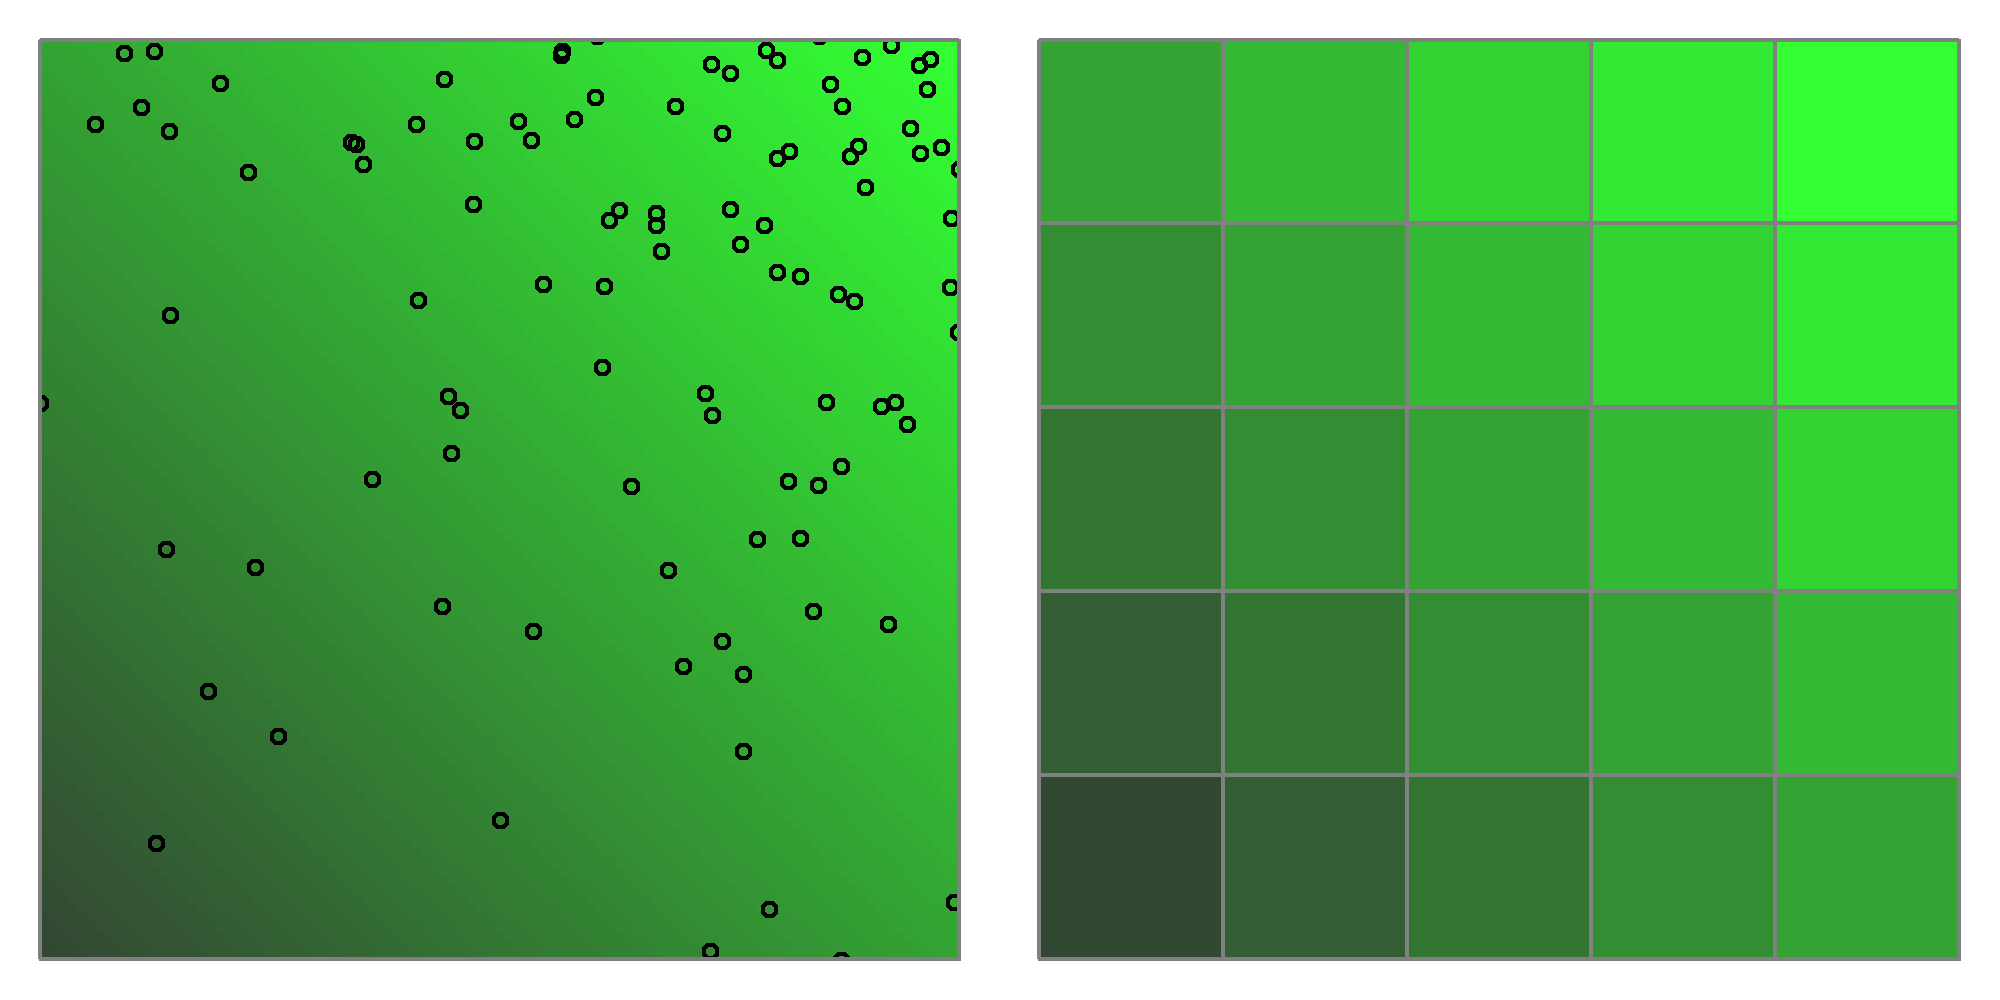
\includegraphics[width=\textwidth]{Ch11/figs/heteroPlots}
\label{state-space.fig.hetero}
\caption{An example of a spatial covariate, say elevation, and a
  realization from an inhomogeneous Poisson point process with
  $\mu(\mathbf{s}, \bm{\beta}) = \exp(\beta_0 + \beta_1
  \mbox{ELEV}(\mathbf{s}))$ where $\beta_0=-6$ and $\beta_1=1$.}
\end{figure}

The 41 simulated points are shown in
Fig~\ref{state-space.fig.hetero}. High elevations
are represented by light gray and low elevations are darker. The
density of points in apparently higher in lighter regions
suggesting that these simulated animals prefer high
elevations.  %Perhaps they are mountain goats.
%The underlying model describing this preference is
%$\log(\mu(s)) = \exp(\beta \times elev(s))$
%where $\beta=2$ is the parameter to be estimated.
Given these points, we will now estimate $\beta_0$ and $\beta_1$ by
minimizing the negative-log-likelihood using \R's \verb+optim+
function.

\begin{samepage}
\begin{small}
\begin{verbatim}
nll <- function(beta) { # negative log-likelihood
    beta0 <- beta[1]
    beta1 <- beta[2]
    EN <- cuhre(2, 1, mu, beta0=beta0, beta1=beta1)$value
    -(sum(beta0 + beta1*elev.fn(s)) - EN)
}
starting.values <- c(0, 0)
fm <- optim(starting.values, nll, hessian=TRUE)
cbind(Est=fm$par, SE=sqrt(diag(solve(fm$hessian)))) # estimates and SEs
\end{verbatim}
\end{small}
\end{samepage}
Maximizing the likelihood took a fraction of a second, and we
obtained estimates of $\hat{\beta}_0=-5.93$ and $\hat{\beta}_1=0.95$,
which are very close to the data generating values. The 95\% confidence
interval for $\hat{\beta}_1$ is [0.61, 1.3] and since it does not
include zero, the null hypothesis that $\beta_1=0$, i.e. that there is
no effect of elevation on density, can be rejected. In addition to testing
hypotheses, these results can be used to predict population size in
new regions or create predicted density surface maps by plugging the
parameter estimates into Eqs.~\ref{state-space.eq.loglin} and~\ref{state-space.eq.EN}.

This example demonstrates
that if we had the data we wish we had, i.e. if we knew the
coordinates of the activity centers, we could easily estimate the
parameters governing the underlying point process and make inferences
about spatial variation in density and abundance. Unfortunately, in
virtually all animal ecology studies, including
SCR, the locations of the $N$ animals, or the $N$ activity centers,
cannot be directly observed. Thus we need
extra information to estimate the locations of these unobserved
points. In SCR, this information comes from the locations where each
animal is captured.

\section{Fitting inhomogeneous point process SCR models}

\subsection{Continuous space}

% One of the nice things about hierarchical models is that they
% %allow us to
% break a complex problem up into a series of simpler conditional
% sub-models. The problem faced in the analysis of SCR data is that the
% underlying point process is not observed, and so an
% observation model is needed to describe how the observed data result from
% the latent activity centers. Thus, in SCR, we can simply add the methods described above into a likelihood
% function or an MCMC algorithm to simulate the posterior distributions of $\beta$ conditional on the
% simulated values of $\mathbf{s}$.

In this example, we will use the same set of points simulated in the
previous section to generate spatial capture-recapture
data. Specifically, we overlay a grid of 49
traps on the map shown in Fig.~\ref{state-space.fig.hetero} and
simulate capture histories conditional upon the activity
centers. Then, we will attempt to estimate the activity center
locations as though we did not know where they were, as is the case in
real applications. We will also estimate $\beta_0$ and $\beta_1$ as
before and see how the estimates compare when the points are not
actually observed. The following \R~code simulates encounter histories under a
Poisson observation model (see Chapt. \ref{chapt.poisson-mn}), which could be appropriate in camera
trapping studies or when using other methods in which animals could
be detected multiple times at a trap during a single occasion.

\begin{samepage}
\begin{small}
\begin{verbatim}
xsp <- seq(20, 80, by=10); len <- length(xsp)
X <- cbind(rep(xsp, each=len), rep(xsp, times=len)) # traps
ntraps <- nrow(X); noccasions <- 5
y <- array(NA, c(N, ntraps, noccasions)) # capture data
sigma <- 5  # scale parameter
lam0 <- 1   # basal encounter rate
lam <- matrix(NA, N, ntraps)
set.seed(5588)
for(i in 1:N) {
    for(j in 1:ntraps) {
        # The object "s" was simulated in previous section
        distSq <- (s[i,1]-X[j,1])^2 + (s[i,2] - X[j,2])^2
        lam[i,j] <- exp(-distSq/(2*sigma^2)) * lam0
        y[i,j,] <- rpois(noccasions, lam[i,j])
    }
}
# data augmentation
nz <- 80; M <- nz+nrow(y)
yz <- array(0, c(M, ntraps, K))
yz[1:nrow(y),,] <- y # Fill data augmentation array
\end{verbatim}
\end{small}
\end{samepage}

Now that we have a simulated capture-recapture dataset \texttt{y} and we have
augmented it to create the new data object \texttt{yz}, we can
estimate the parameters using MCMC.  A commented Gibbs sampler written
in \R~is available in the accompanying \R~package \scrbook~(see
\texttt{?scrIPP}). This function is not meant to be an all purpose
tool for fitting SCR models using MCMC---instead, it is presented so
that interested readers can better understand the computational
aspects of the problem and can modify it for their purposes.
The function can be used as so:
%\begin{samepage}
\begin{small}
\begin{verbatim}
set.seed(3434)
fm1 <- scrIPP(yz, X, M, 10000, xlims=c(0,100), ylims=c(0,100),
              space.cov=elev.fn,
              tune=c(0.4, 0.2, 0.3, 0.3, 7))
plot(mcmc(fm1$out))
\end{verbatim}
\end{small}
%\end{samepage}
which requests 10000 posterior samples and estimates the effect of the
spatial covariate, elevation, on density. Currently, the function
places uniform priors on the parameters $\sigma$, $\lambda_0$,
$\beta_0$ and $\beta_1$, although this could easily be modified. Note that any spatial
covariate that returns a real value for any location in the
state-space can be supplied using the \texttt{space.cov} argument. The resulting
trace plots of the Markov chains and the posterior distributions for
three parameters are
shown in Fig.~\ref{state-space.fig.fm1post}. The chains appear to
converge rapidly but may need to be run longer to reduce Monte Carlo
error.

\begin{figure}
  \centering
  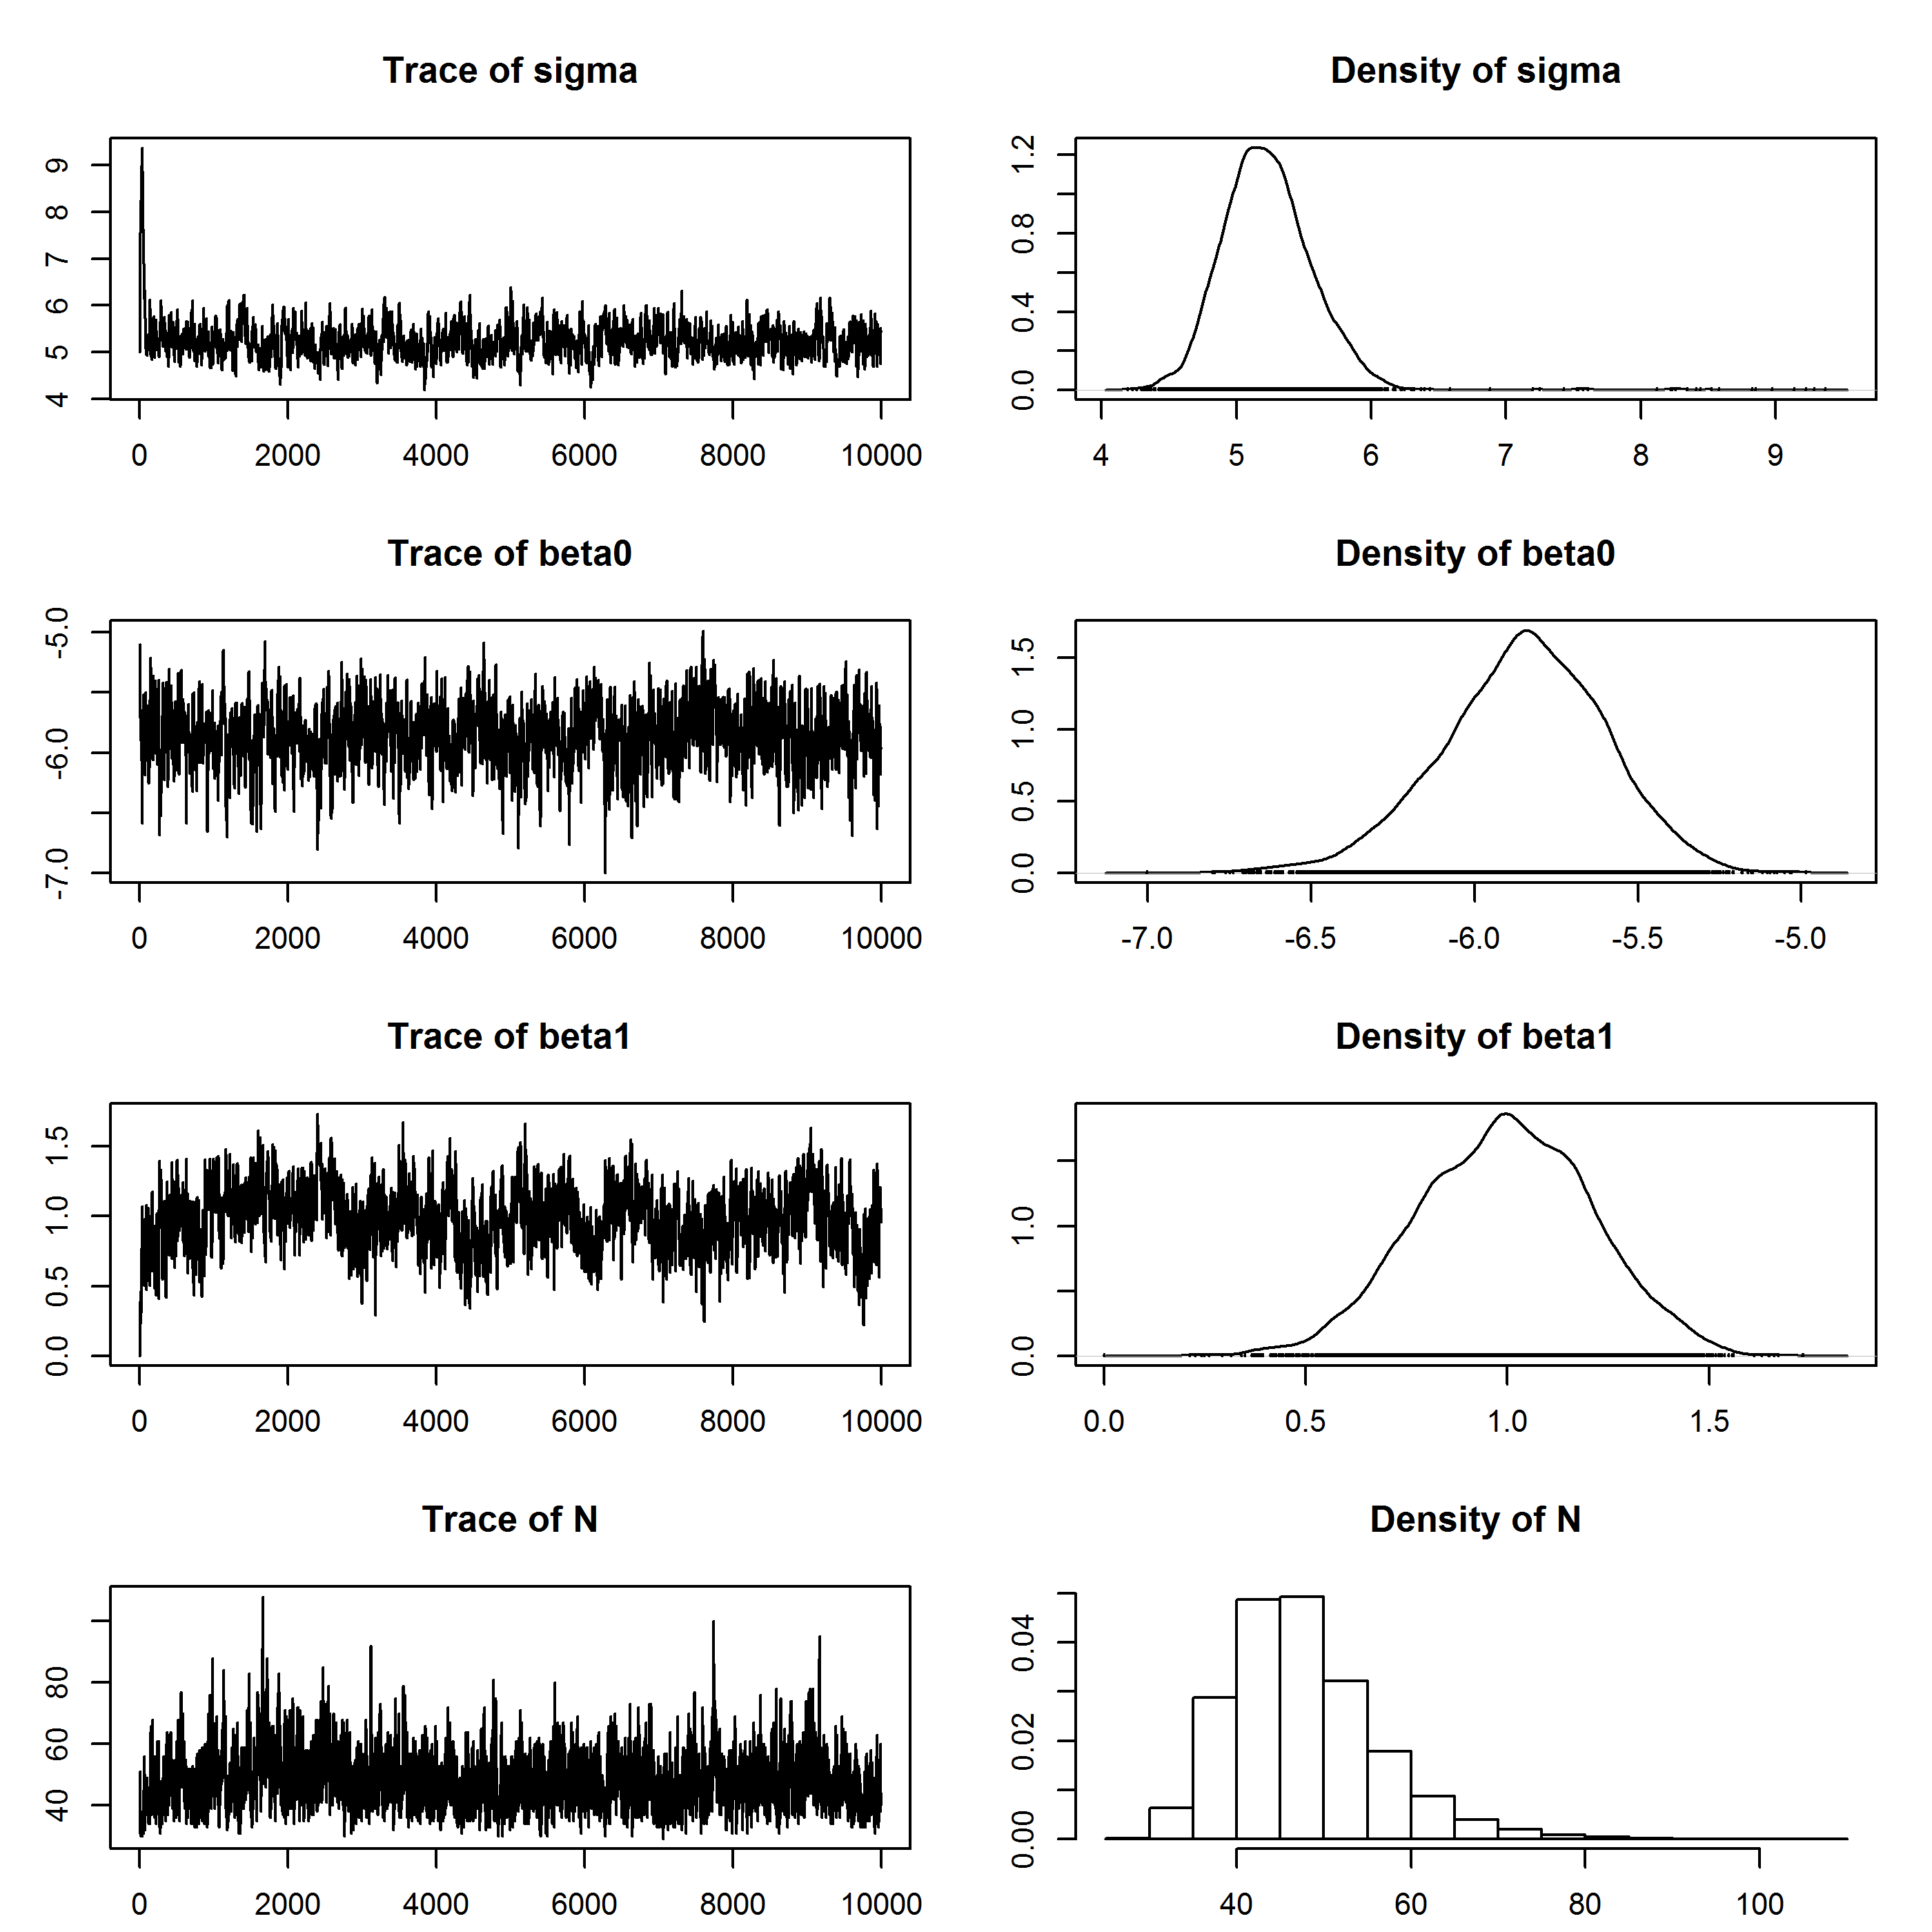
\includegraphics[width=0.8\textwidth]{Ch11/figs/fm1p}
  \caption{Trace plots and posterior distributions from MCMC analysis
    of SCR model with inhomogeneous point process. Analysis was
    conducted using the \texttt{scrIPP} function in the accompanying
    \R~package \scrbook.}
  \label{state-space.fig.fm1post}
\end{figure}
%For comparison, we also fit this model using $\texttt{secr}$. See the
%help file \texttt{Ch-IPP} in \scrbook~ for \R~commands necessary to
%prepare the data for \secr.

\begin{table}%[b]
\centering
\caption{Summary of posterior distributions from SCR model with
  inhomogeneous point process. }
\begin{tabular}{lrrrr}
\hline
Parameter 	 	& Mean  	& SD    	& 2.5\% 	& 97.5\% \\
\hline
 $\sigma=5$ 	 	&  5.232 	&  0.310 	&  4.681 	&  5.858 \\
 $\lambda_0=1$ 	 	&  0.802 	&  0.119 	&  0.595 	&  1.049 \\
 $\beta_0=-6$ 	 	& -5.856        & 0.2542        & -6.376        & -5.393 \\
 $\beta_1=1$ 	 	&  0.985 	&  0.209 	&  0.575 	&  1.378 \\
 $N=41$ 	 	& 47.615 	&  8.041 	& 35.000 	& 66.000 \\
 $\mathbb{E}[N]=39.9$ 	& 47.551 	& 10.992 	& 29.837 	& 71.332 \\
\hline
\end{tabular}
\label{state-space.tab.simIPP}
\end{table}

Summaries of the posterior distributions are presented in
Table~\ref{state-space.tab.simIPP}. The posterior means for $\beta_0$
and $\beta_1$ are quite similar to MLEs from the analysis in the
previous section in which we assumed no observation error. However, we
see that the confidence intervals are wider. With respect to the other
parameters in the model, we see that all of the data
generating parameter fall within the 95\% credible intervals. One
interesting thing to note is that, although the point estimates for
the expected and realized values of $N$ are quite similar, the
estimate is more precise for the realized value. This is to be
expected because the uncertainty associated with the realized value of
$N$ is entirely determined by the encounter rate parameters. That is,
if we could perfectly detect all of the individuals in $\cal S$, there
would be no uncertainty about $N$. In contrast, the variance for
expected value of $N$ is affected by the variance of all the parameters
in the model, not just the encounter rate parameters. See
\citet{efford_fewster:2012} for additional discussion on the
difference between realized and expected values of abundance.
%, and we see that the point
%estimates and confidence/credible intervals are quite similar from the
%MCMC and maximum likelihood (ML) analyses. One exception is that the
%confidence intervals for $N$ and the expected value of $N$ are
%somewhat different. This may result from the fact that the MCMC
%analysis assumed a binomial prior for $N$, whereas the ML analysis
%assumed a Poisson prior.


Fitting continuous space inhomogenous point process models is somewhat
difficult in \bugs~because the ``IPP'' prior $[\mathbf{s}_i | \bm
\beta]$---unlike the uniform prior---is not one of the
available distributions that comes with the software. It is
possible to add new distributions in \bugs, but it is somewhat
cumbersome.  \secr~allows
users to fit continuous space models using linear or polynomial functions of the x- and y-
coordinates, but it does not accept truly continuous covariates that
are functions of space. However, these
are not really important limitations because discrete
space versions of the model are straight-forward, and virtually all spatial
covariates are, or can be, defined as such.

\subsection{Discrete space}
\label{modeling.sec.discrete}

To fit inhomogeneous point process models using covariates in discrete
space, i.e. in raster format, we follow the same steps
as outlined in Chapter~\ref{chapt.poisson-mn}---we define ${\bf s}_i$ as
pixel ID, and we use the categorical distribution as a prior. This
effectively changes the problem from estimating the coordinates of an
activity center, to estimating the pixel in which an activity center is
located. As pixel size approaches zero, these two become equivalent. A good
example is found in \citep{mollet_etal:2012}. Here we present
an analysis of the simulated data shown in the %right panel of
Fig.~\ref{state-space.fig.hetero}. The spatial covariate, let's call it
forest canopy height (CANHT), was simulated
using using the code shown on the help page
\verb+ch11+ in \scrbook. The points are the number of
activity centers in each pixel, generated from a single realization of
the inhomogeneous point process model with intensity
$\mu(\mathbf{s}, \bm{\beta}) = \exp(\beta_0 + \beta_1
\text{CANHT}({\bf s}))\times\text{pixelArea}$,
where $\beta_0 = -6$ and $\beta_1 = 1$.
\begin{figure}[ht]
\centering
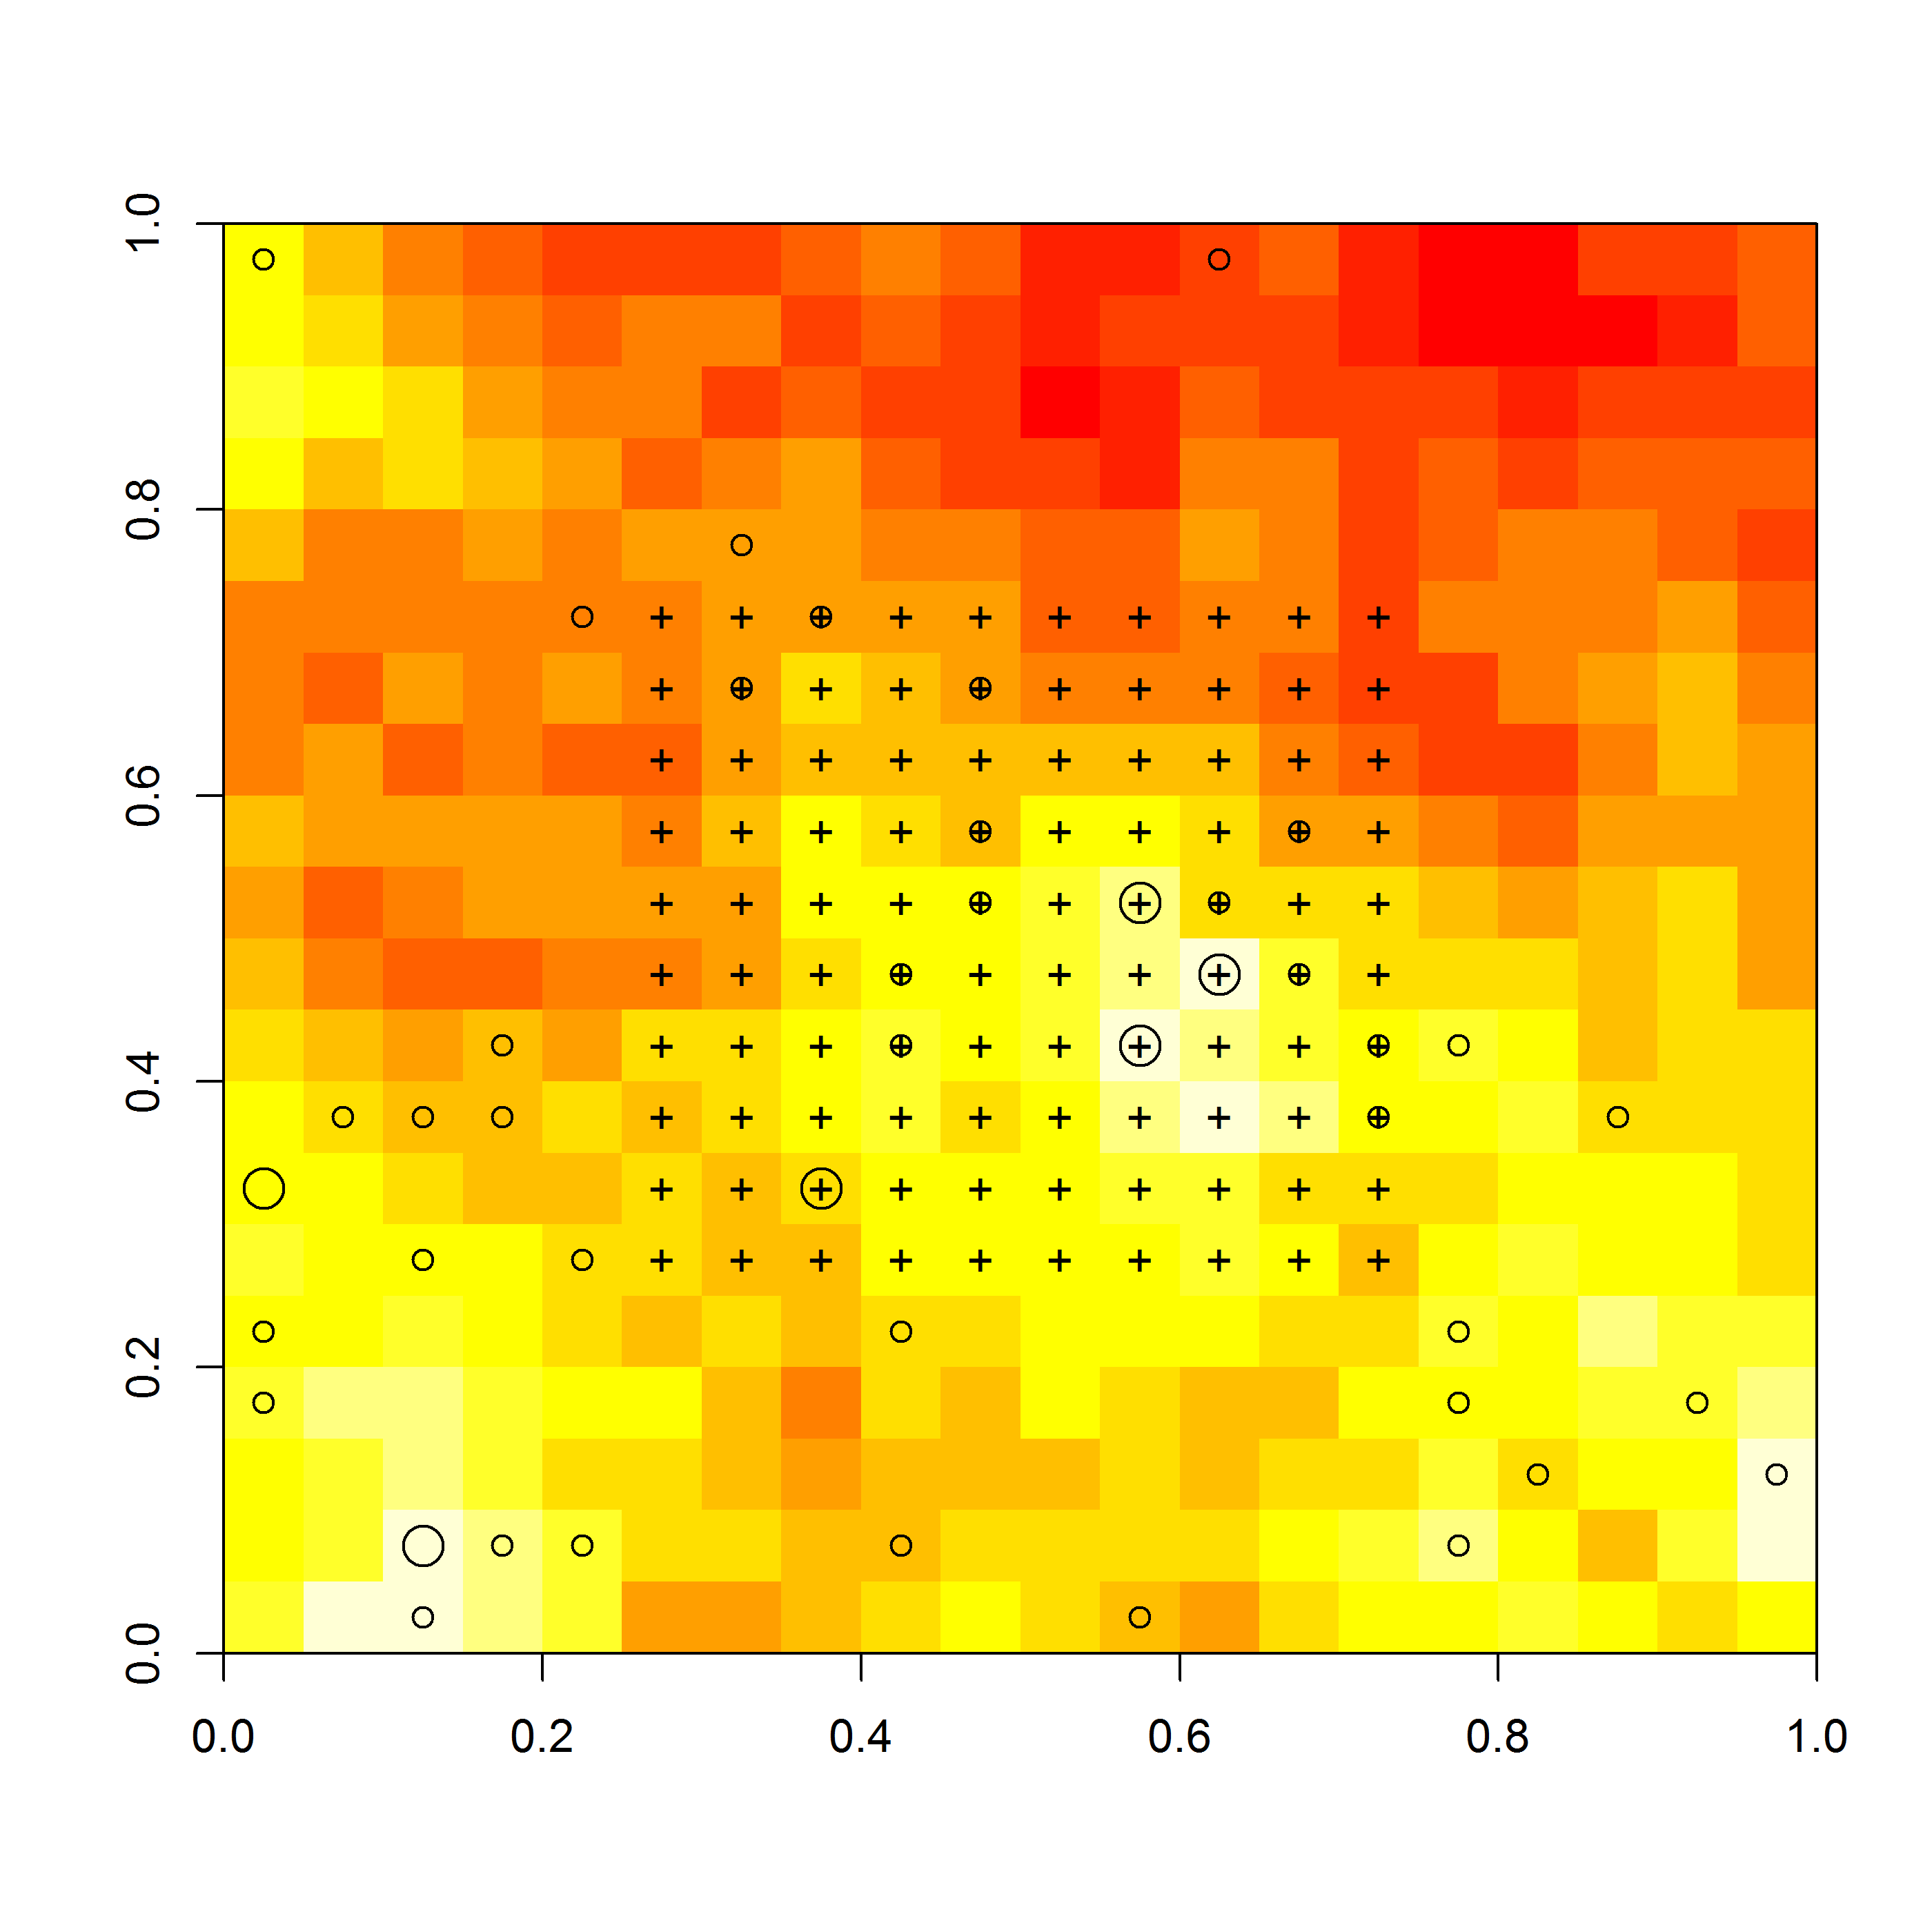
\includegraphics[width=0.6\textwidth]{Ch11/figs/discrete}
\label{state-space.fig.discrete}
\caption{Simulated activity centers in discrete space. The spatial
  covariate, canopy height, is highest in the lighter areas and
  density increases with canopy height. A single
  activity center is shown as a small circle, and larger circles
  represent two activity centers in a pixel. Trap locations
  are shown as crosses.}
\end{figure}

The \bugs~description of the model is shown in
panel~\ref{state-space.panel1}. The vector \verb+probs[]+ is the prior
probability defined by Eq.~\ref{state-space.eq.pdf.hetero.d}, which is
the probability that an individual's activity center is located at
pixel $\bf s$. \verb+Sgrid+ is the matrix of coordinates for each pixel.

\begin{panel}%[h!]
\centering
\rule[0.15in]{\textwidth}{.03in}
\begin{small}
\begin{verbatim}
model{
sigma ~ dunif(0, 20)
lam0 ~ dunif(0, 5)
beta0 ~ dunif(-10, 10)
beta1 ~ dunif(-10, 10)
for(j in 1:nPix) {
  mu[j] <- exp(beta0 + beta1*CANHT[j])*pixArea
  probs[j] <- mu[j]/EN
}
EN <- sum(mu[]) # Expected value of N, E[N]
psi <- EN/M
for(i in 1:M) {
  w[i] ~ dbern(psi)
  s[i] ~ dcat(probs[])
  x0g[i] <- Sgrid[s[i],1]
  y0g[i] <- Sgrid[s[i],2]
  for(j in 1:ntraps) {
    dist[i,j] <- sqrt(pow(x0g[i]-traps[j,1],2) + pow(y0g[i]-traps[j,2],2))
    lambda[i,j] <- lam0*exp(-dist[i,j]*dist[i,j]/(2*sigma*sigma)) * w[i]
    y[i,j] ~ dpois(lambda[i,j])
    }
  }
N <- sum(w[]) # Realized value of N
}
\end{verbatim}
\end{small}
\rule[0.15in]{\textwidth}{.03in}
\caption{\bugs~code for fitting inhomogeneous point process model in
  discrete space.}
\label{state-space.panel1}
\end{panel}

This model can also be fit in \secr, which refers
to the raster data as a ``habitat mask''. \R~code to format the data
and fit the models using \secr~and \jags~is available in \scrbook---see
\verb#help(ch9secrYjags)#. Results of the
comparison are shown in Table \ref{state-space.tab.jagsVsecr} and are
similar as expected. The differences that do exist can be
explained by a variety of reasons. For one, there exists some Monte
Carlo error in the Bayesian posterior summaries. There is also the
fact that posterior summaries can be computed in numerous ways---for
example, we could have presented posterior modes or medians instead of
means---or, we could have shown highest posterior density credible
intervals instead of simple percentiles. The posteriors would also
differ if we chose more informative priors than the uniform
distributions used here. We see no reason why these
issues should be seen as limitations of the Bayesian analysis, rather
we would argue that the posterior distribution, which describes the
probability that the parameter equals any particular value, is a
better descriptor uncertainty than any particular point estimator or
confidence interval. %Futhermore, most of these differences are minor,
%and hardly worth mention.
% The only exception is that the estimates of
% the expected and realized values of $N$ are closer to the data
% generating values in the Bayesian analysis, and the Bayesian credible
% intervals are narrower than the frequentist confidence intervals. This
% is likely a result of the fact that the Bayesian analysis assumed
% that $N$ was binomial whereas the frequentist analysis
% assumed a Poisson prior for $N$, and the variance of the binomial will
% always be less than or equal to the variance of Poisson distribution
% for a shared expectation.

\begin{table}%[h!]
\centering
\caption{Comparison of \secr~and \jags~results. Point estimates from
  the Bayesian analysis are posterior means. Intervals are lower and
  upper 95\% CIs.}
\begin{tabular}{lrlrrrr}
\hline
Parameter 	& Truth 	& Software 	& Mean 	& SD 	& 2.5\% & 97.5\% \\
\hline
 $\lambda_0$ 	&  1.00 	& \textbf{JAGS} 	&  1.04 	& 0.087 	&  0.88 	&  1.22 \\
  	&  1.00 	& \texttt{secr} 	&  1.08 	& 0.089 	&  0.92 	&  1.27 \\
 $\sigma$ 	& 10.00 	& \textbf{JAGS} 	& 10.16 	& 0.373 	&  9.46 	& 10.94 \\
  	& 10.00 	& \texttt{secr} 	&  9.84 	& 0.350 	&  9.18 	& 10.55 \\
 $\beta_1$ 	&  1.00 	& \textbf{JAGS} 	&  1.20 	& 0.350 	&  0.50 	&  1.88 \\
  	&  1.00 	& \texttt{secr} 	&  1.09 	& 0.316 	&  0.47 	&  1.71 \\
 $N$ 	& 30.00 	& \textbf{JAGS} 	& 26.63 	& 2.585 	& 23.00 	& 33.00 \\
  	& 30.00 	& \texttt{secr} 	& 28.19 	& 3.037 	& 24.49 	& 37.39 \\
 $\mathbb{E}[N]$ 	& 32.30 	& \textbf{JAGS} 	& 26.39 	& 5.048 	& 17.25 	& 36.96 \\
  	& 32.30 	& \texttt{secr} 	& 28.19 	& 6.117 	& 18.52 	& 42.93 \\
\hline
\end{tabular}
\label{state-space.tab.jagsVsecr}
\end{table}


\section{Ecological Distance and Density Covariates}

Habitat characteristics that affect spatial variation in density can
also affect home range size and movement behavior. For example, a
species that occurs at high density in a forest may be reluctant to
venture from a forest patch into an adjacent field. Thus, even if a
trap placed in a field is located very close to an animal's activity
center, the probability of capture may be very
low. In this case, forest cover is a covariate of
both density and encounter probability,
and we could model it as such by combining the methods described in
this chapter with those described in Chapter~\ref{chapt.ecoldist}.

To demonstrate, we continue with our analysis of the data shown in
Fig~\ref{state-space.fig.discrete}. Once again, we suppose that density
increases with canopy height, but this time, we also make the
assumption that home range size decreases as density increases. This
commonly-observed phenomenon can be explained by numerous factors such
as intra-specific competition \citep{sillett_etal:2004} or optimal
foraging behavior \citep{tufto_etal:1996,said_servanty:2005}. To model
this effect, we
introduce the parameter $\theta$, which determines the ``cost'' of
moving between pixels. If $\theta=0$, then the animal perceives
distance as Euclidean. If $\theta>0$, then least-cost distance (LCD)
is greater than than Euclidean distance (ED). In most cases, we would
not expect,
or should not even consider the possibility of $\theta<0$ because this
implies that LCD$<$ED, which would mean that an animal could view
1000km as 1m. In addition to the fact that this is not biologically
justifiable, it also suggests that the area of the state-space could
be infinitely large. Thus, one may want to enforce the constraint that
$\theta$ is $\geq 0$. See Chapter~\ref{chapt.ecoldist} for
more details.

A question that arises is: Is possible to estimate $\bm \beta$
and $\theta$ using standard SCR data? In other words, can we model
spatial variation in density and connectivity at the same time,
using standard SCR data? Currently, it is not possible to
model least-cost distance using \jags~or \secr, so we wrote our own
function, \verb+scrDED+, to fit the model using maximum likelihood. An
example analysis is provided on the help page for the function in our
\R~package \scrbook. We briefly note here that the function requires
the capture history data, the trap locations, and the raster data
formatted using the {\tt raster} package
\citep{hijmans_vanetten:2012}. The linear model for the
intensity parameter $\mu(\mathbf{s}, \beta)$ and the least-cost distance
function $\text{lcd}(\theta)$ are specified using \R's formula interface. A
simple function call is
\begin{verbatim}
fm <- scrDED(y, traplocs=X, den.formula=~elev, dist.formula=~elev,
             rasters=elev.raster)
\end{verbatim}
To assess the possibility of estimating both $\bm \beta$ and $\theta$, we
conducted a small simulation study, generating 500 datasets from the
model with both parameters set to 1, which corresponds to the
conditions described above. The results indicate that it is
possible to estimate both parameters
(Fig~\ref{ch9.fig.sim}).

\begin{figure}[ht]
\centering
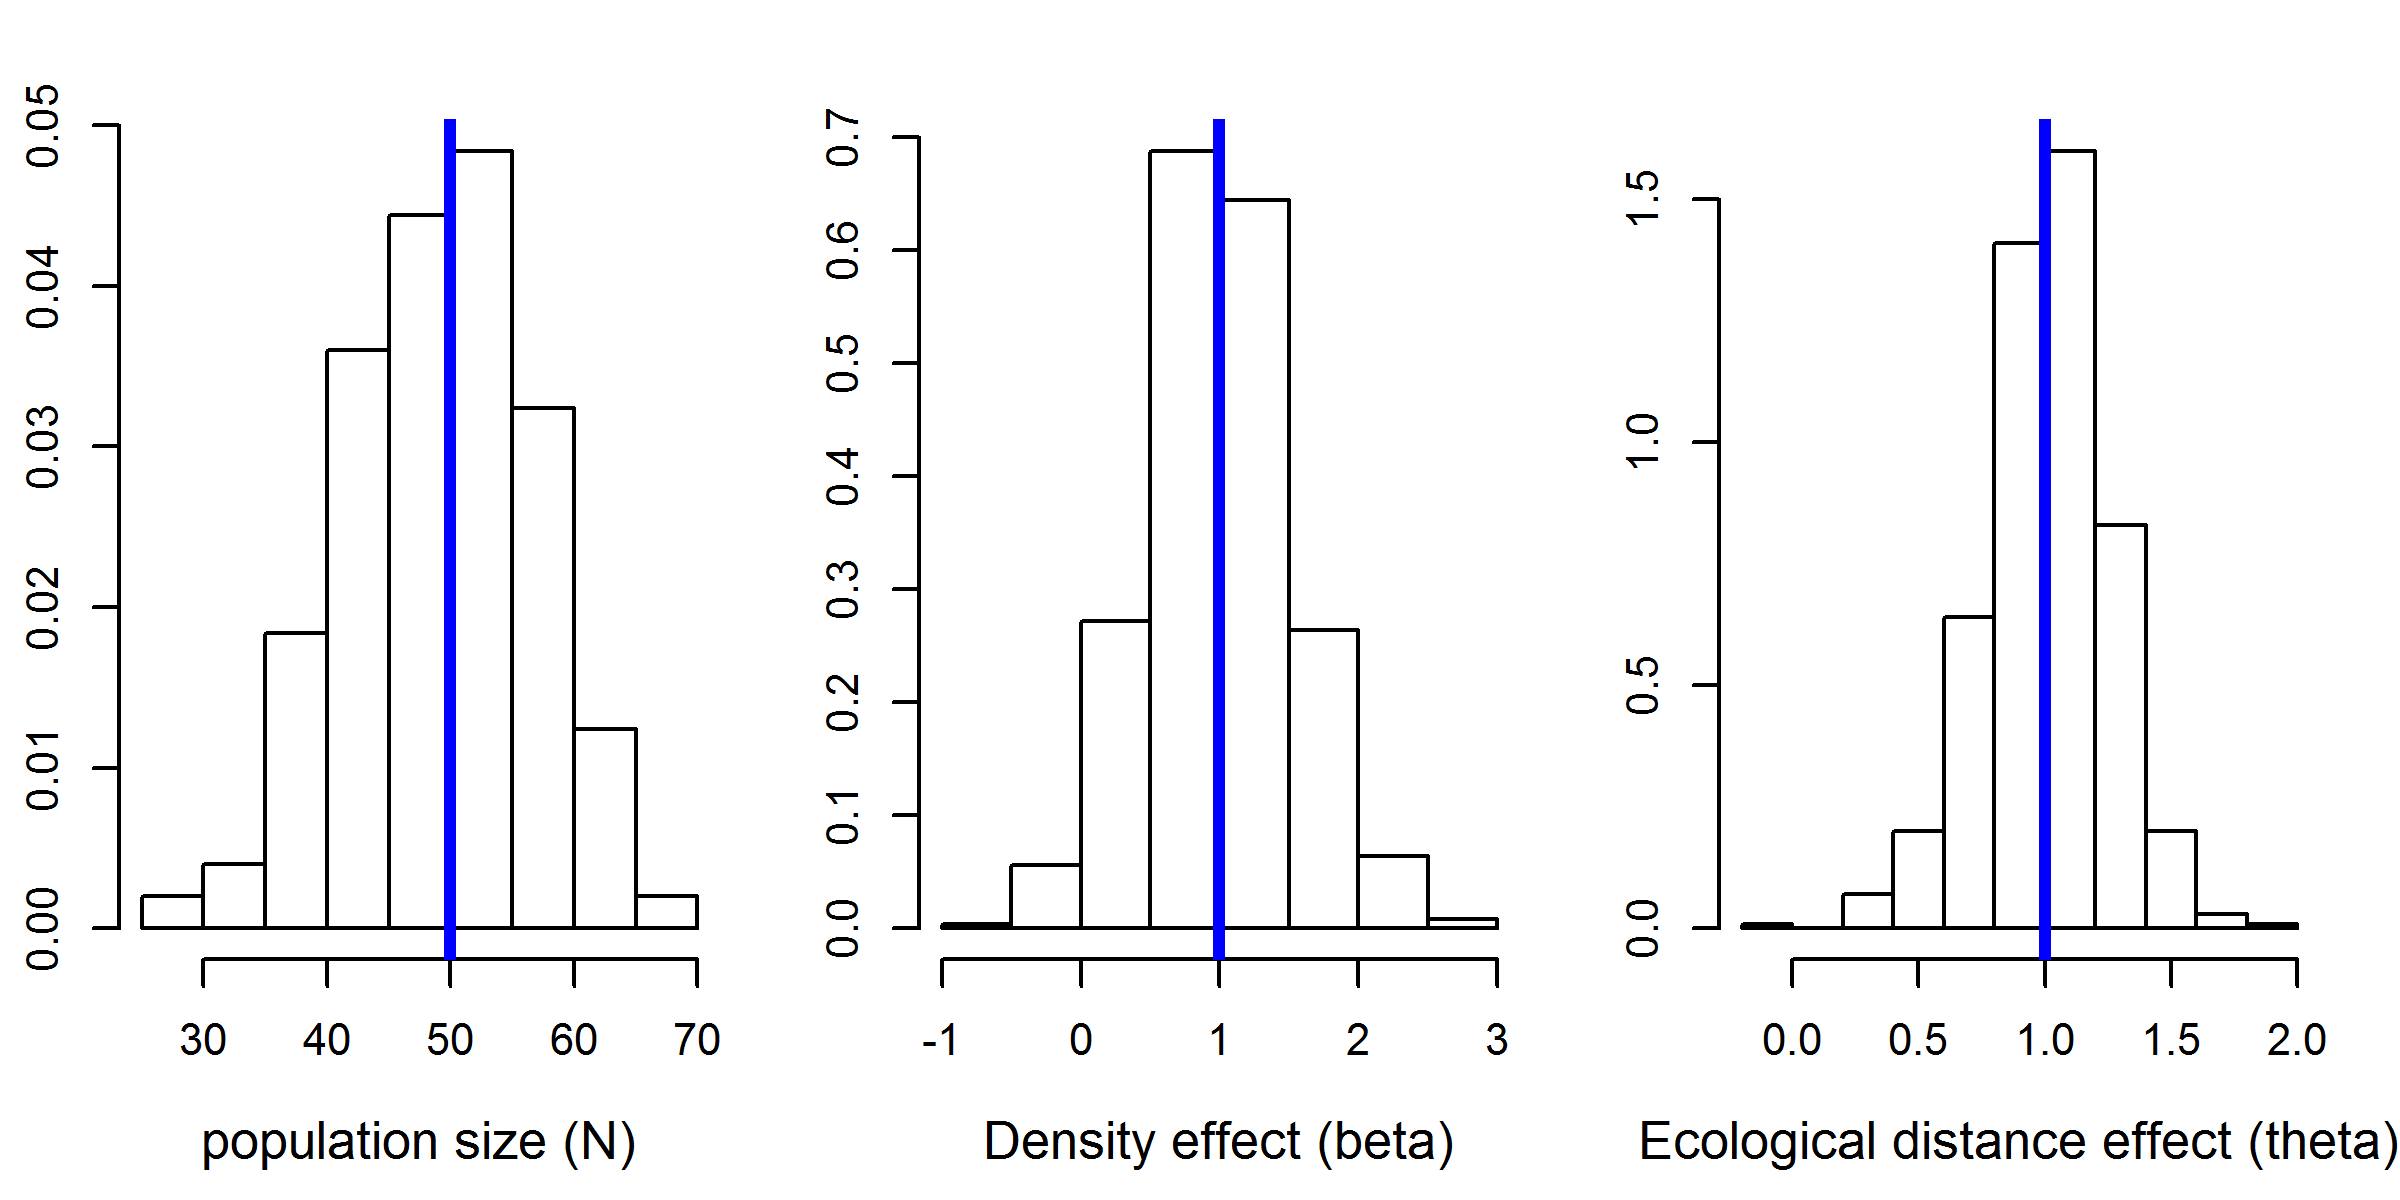
\includegraphics[width=4in,height=2in]{Ch11/figs/scrDEDsim}
\caption{Histograms of parameter estimates from 500 simulations under
  the model in which both density and ecological distance are affected
by the same covariate, canopy height. The vertical lines indicate the
data-generating value.}
\label{ch9.fig.sim}
\end{figure}


\section{The Jaguar Data}

Estimating density of large felines has been a priority for many
conservation organizations, but few robust methodologies existed before
the advent of SCR. Distance sampling is not feasible for such rare and
cryptic species, and traditional capture-recapture methods yield
estimates that are highly sensitive to the subjective choice of the
effective survey area. SCR models provide a powerful alternative
because density can be estimated directly and data can be collected
using non-invasive methods such as camera traps or hair snares.

In this example, we demonstrate how readily density can be estimated
for a globally imperiled species using SCR. Furthermore, we show how
inhomogeneous point process models can be used to test important
hypotheses regarding the factors affecting density.
The data come from an 8-year camera-trapping study designed to assess the impacts of poaching
on jaguar density in Argentina, near the borders of Brazil and
Paraguay. Additional information about the study is presented in
\citet{paviolo_etal:2008} and \citet{paviolo_etal:2009}. Although
jaguars themselves are occasionally killed by
poachers, the larger concern is the influence of poaching on prey
species. To protect jaguars and related species, protected areas have
been established and three levels of protection are
recognized as depicted in Fig.~\ref{state-space.fig.jaguarCts}. The dark green
area is the Iguaz\'{u} National Park that is patrolled regularly by law enforcement
officials. The light green areas are officially protected, but due to
resource limitations, are not patrolled as often. The beige areas are
not protected at all, and the gray areas are large soybean
monocultures, which provide no habitat.

To test for differences in
density between the three regions, we modeled the point process intensity parameter
as a function of protection status (PROTECT), which we treated as an
ordinal variable: $\mu(\mathbf{s}, \bm{\beta}) = \exp(\beta_0 +
\beta_1\text{PROTECT}(\mathbf{s}))$. We hypothesized that $\beta_1 > 0$
indicating that jaguar density increases with protection status. In
addition to modeling spatial variation in density, we also modeled the
scale parameter of the half-normal or Gaussian encounter model as
sex-specific, since male cats typically have larger home ranges than
females \citep{sollmann_etal:2011}. Since sex is an
individual-specific covariate, and not observed for the individuals
that were not captured, a prior is required for the sex of uncaptured
individuals. We used an Bernoulli prior with probability 0.5 to
describe our uncertainty about sex ratio.

\begin{figure}%[ht]
\centering
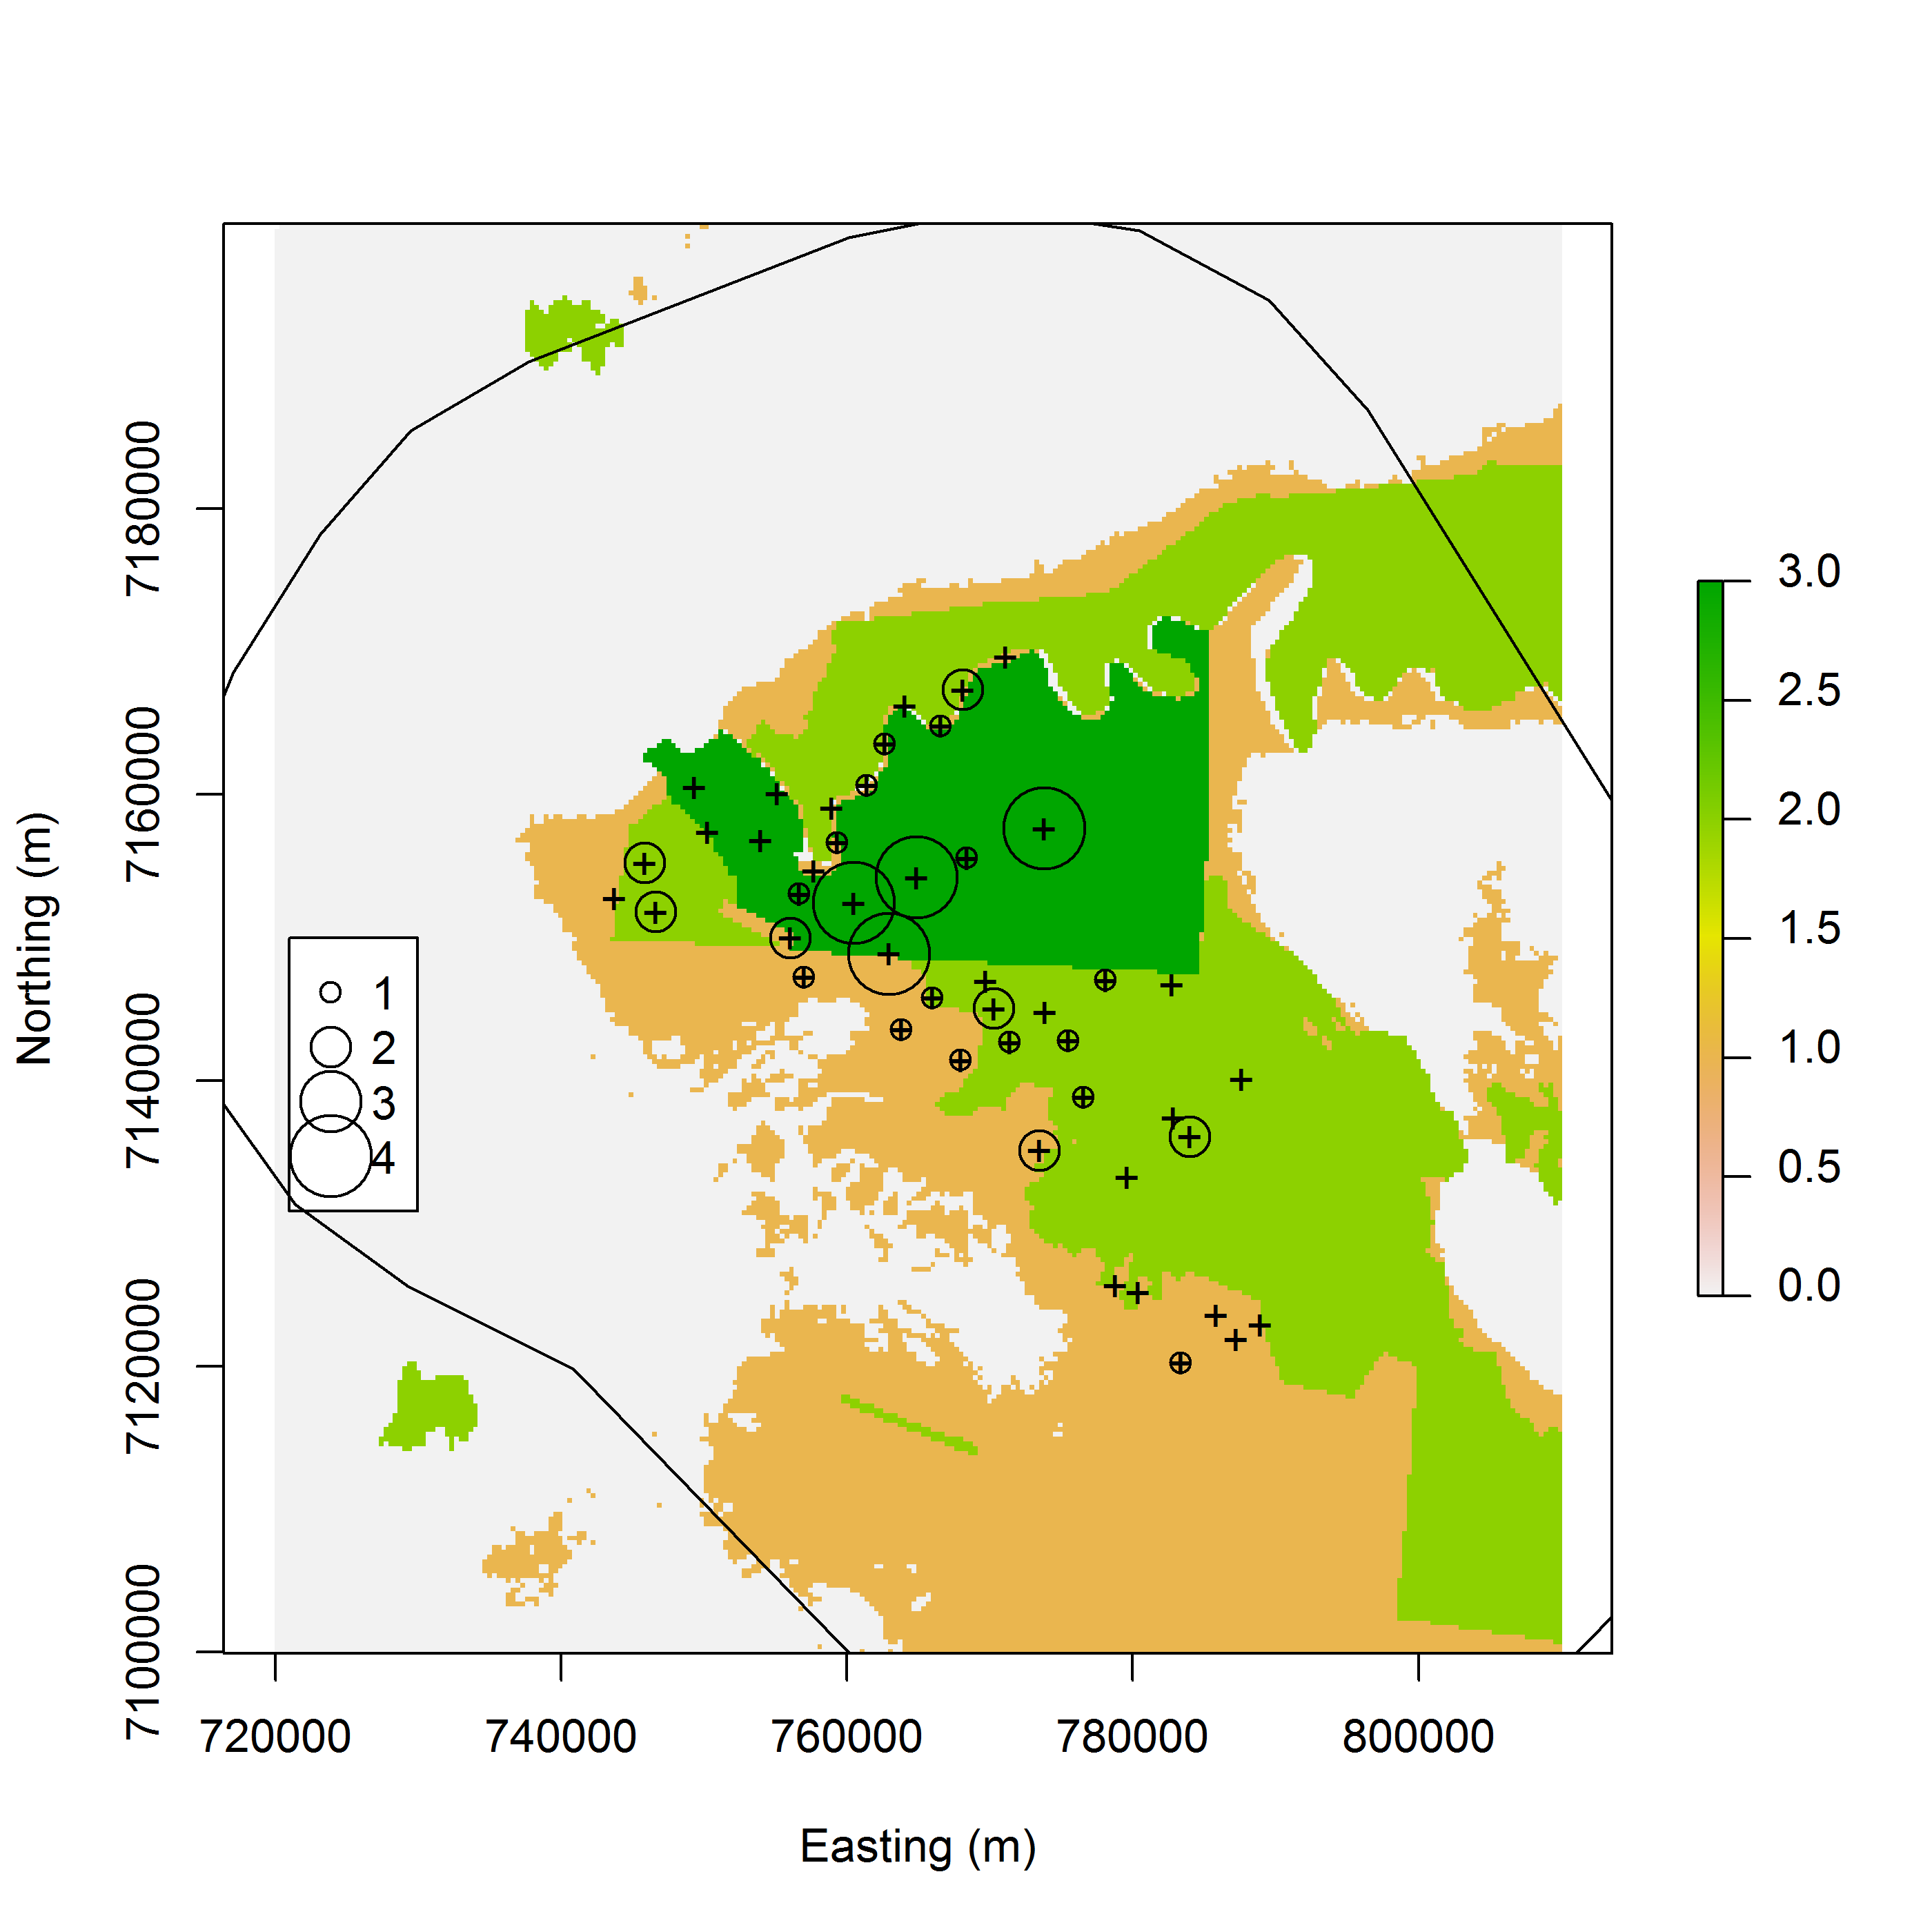
\includegraphics[width=0.6\textwidth]{Ch11/figs/jaguarCountMap}
\label{state-space.fig.jaguarCts}
\caption{Jaguar detections at 46 camera trap stations. The three levels of
  protection status are no protection (beige), some protection (light
  green), and Iguaz\'{u} National Park (dark green). Non-habitat
  (soybean monocultures) is shown in gray. }
\end{figure}

The geometry of the state-space differs greatly from the simple square
regions that we have considered throughout this chapter, which raises
a few questions. First, how would one integrate
Eq.~\ref{state-space.eq.pdf.hetero} over a
complex spatial region? Earlier we used the function \verb+cuhre+ in
\R~for the two-dimensional integration, but its \verb+lower+ and
\verb+upper+ arguments essentially assume that the state-space is
square. There are methods of transforming the state-space to make this
work, but once again we find that it is most convenient to work in
discrete space and sum over all the pixels defining
$\mathcal{S}$. In this example, we restricted the state-space to exclude the large
soybean monocultures surrounding the study area, and we only
considered area south of the Iguaz\'{u} River, which runs along the northern border
of the park shown in dark green in
Fig.~\ref{state-space.fig.jaguarCts}. Rather than restricting the
state-space, we could have modeled the permeability of the river using
the methods described in the previous section and in
Chapter~\ref{chapt.ecoldist}; however, no sampling was conducted on
the northern side of the river, and ancillary data indicates that
jaguars rarely forge the waterway.

We fit the model to data from a single year of data from 46
camera stations, each consisting of a pair of cameras placed along
roads or small trails. Forty-five detections of 16 jaguars (8 males and 8
females) were made over a 95-day sampling period. The mean number of
sampling days at each camera station was 48.2. The raw capture data
shown in Fig.~\ref{state-space.fig.jaguarCts} suggest that the highest
number of captures was in the national park, but there were also
several traps in the park with no captures. Furthermore, few cameras
were placed far from the protected areas, making it somewhat difficult
to detect differences in density. \R~code to fit the model is
available in \scrbook  on the help page \verb+jaguarDataCh9+.
Parameter estimates are shown in Table\ref{state-space.tab.jagposts}.


% To assess the influence of poaching on jaguar density, we treated
% protection status as an ordinal variable with 3 levels: no protection,
% some protection, and high protection (national parks). Clearly these
% are ordered, and our
% hypothesis is that poaching pressure should decrease and jaguar
% density should increase with the level of
% protection. Thus, $\beta$ in this example is a ``slope''
% parameter describing the degree to which protection status affects
% jaguar density. We also hypothesized that males would have larger home
% ranges than females  and that the sex ratio may not be
% 1:1.


\begin{table}
\centering
\caption{Summaries of posterior distributions from the model of jaguar
  density. $\sigma$ is the scale parameter of
  the half-normal detection function. $\rho$ is the
  sex-ratio. $\lambda_0$ is base-line encounter rate. $\beta$ is the
  effect of protection on jaguar density. D is the overall density
  estimate. D1, D2, and D3 are the density estimates
  (jaguars/100km$^2$) for the three levels of protection. }
\begin{tabular}{lrrrr}
\hline
& Mean & SD & 2.5\% & 97.5\% \\
\hline
 $\sigma_\text{female}$ 	& 5691.801 	& 1042.6666 	& 4076.2436 	& 8196.44 \\
 $\sigma_\text{male}$ 	& 6324.799 	&  886.6015 	& 4868.9539 	& 8322.95 \\
 $\lambda_0$ 	&    0.012 	&    0.0036 	&    0.0063 	&    0.02 \\
 $\psi$ 	&    0.357 	&    0.1119 	&    0.1892 	&    0.62 \\
 $\beta_0$ 	&   -4.675 	&    0.2813 	&   -5.2637 	&   -4.13 \\
 $\beta_1$ 	&    0.236 	&    0.3594 	&   -0.4154 	&    0.95 \\
 $N$ 	&   35.673 	&    9.2778 	&   22.0000 	&   58.00 \\
 $N_\text{male}$ 	&   19.412 	&    5.7245 	&   11.0000 	&   33.00 \\
 $D_\text{low}$ 	&    0.885 	&    0.3706 	&    0.3315 	&    1.80 \\
 $D_\text{med}$ 	&    0.769 	&    0.2872 	&    0.2653 	&    1.41 \\
 $D_\text{high}$ 	&    1.459 	&    0.3360 	&    0.8791 	&    2.11 \\
 \hline
\end{tabular}
\label{state-space.tab.jagposts}
\end{table}

The results indicate that efforts to protect jaguars by reducing
poaching in protected areas are not working as well as hoped
for. \hl{WAITING ON FINAL RESULTS: The
posterior probability that $\beta_0 > 0$ was XXXX, and
the posterior mean of realized density was only XXXX\%} higher in the national park than in the
unprotected area. Fig.~\ref{state-space.fig.Dsurface} shows the estimated
density surfaces. The first map is the expected density (posterior mean) in each of
the three values, which was computed by plugging in the posterior mean
values of $\beta_0$ and $\beta_1$ into the log-linear intensity
function. The second map is the realized density surface. Conditional
on the $N$, this is the probability distribution for the
number of activity centers in each pixel of the rasterized
state-space---here shown as the posterior mean. The expected values
would be used if we were interested in making inferences about other
areas or time periods, whereas the realized map is the best
description of the system during the study period.

\begin{figure}%[ht]
\centering
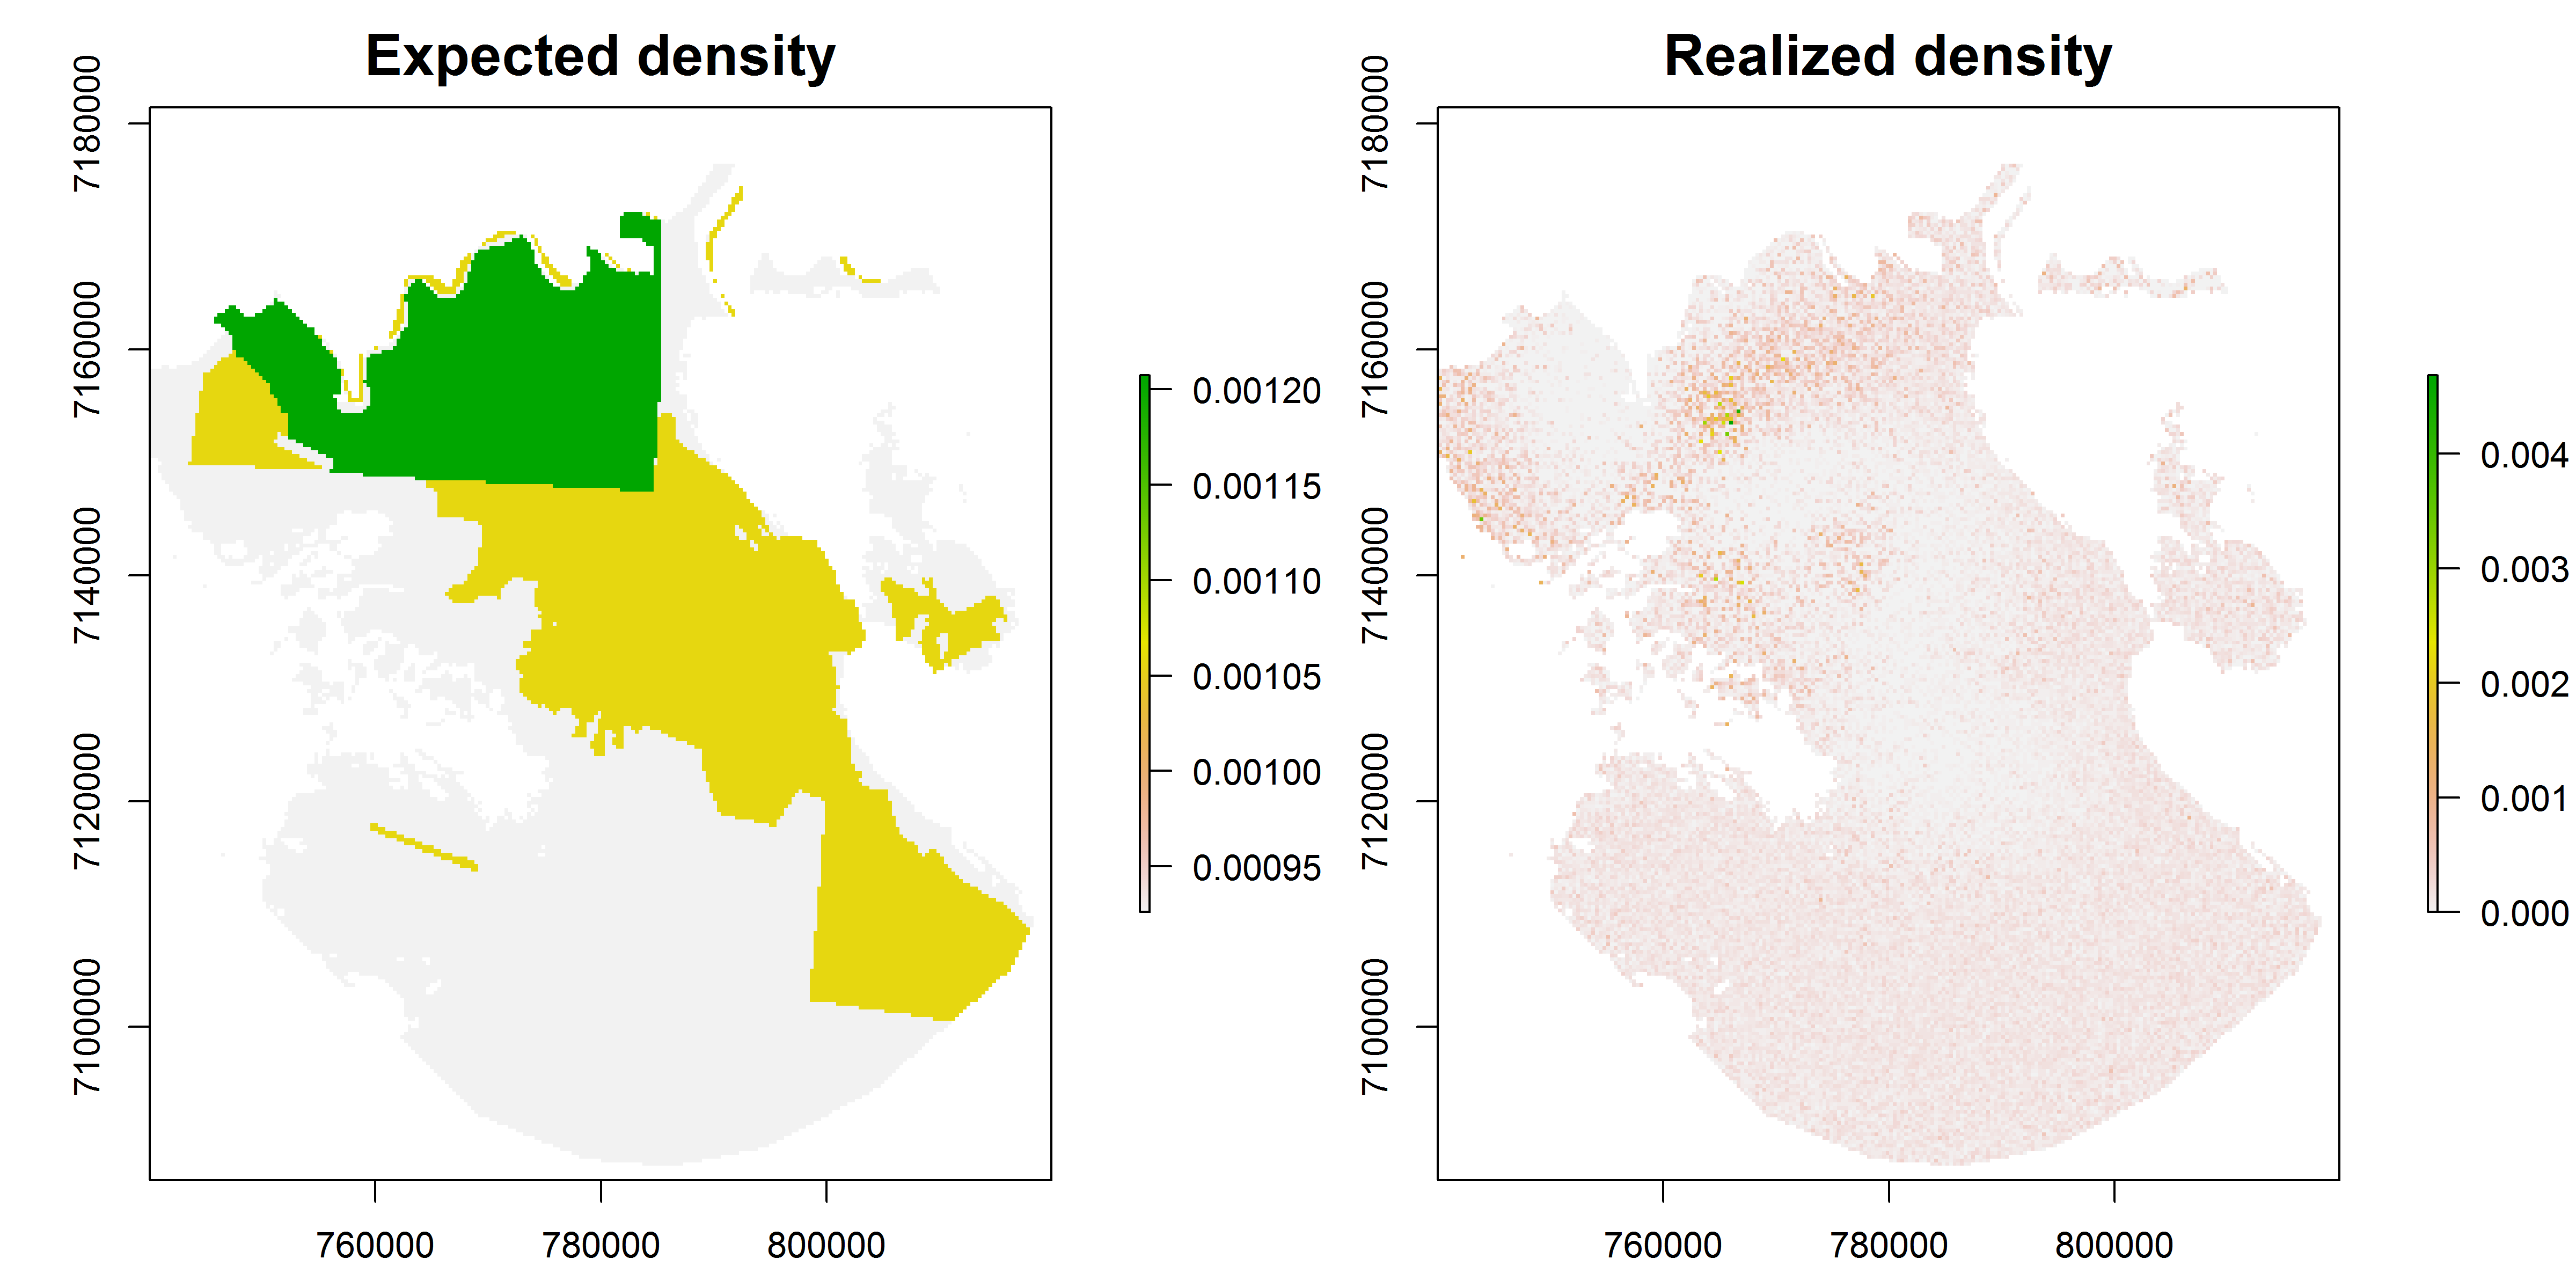
\includegraphics[width=\textwidth]{Ch11/figs/reD}
\label{state-space.fig.Dsurface}
\caption{Estimated density surfaces from the analysis of the jaguar data.}
\end{figure}

We note that there is room for improvement in our analysis and our
results should be considered preliminary. The
political boundaries used to demarcate protected areas are not as
concrete as we might like. In reality poaching pressure is likely
higher near remote park boundaries than in well-guarded park
interiors. One option for addressing this would be to use a continuous
measure of poaching pressure such as distance from the nearest town,
or some other accessibility metric. It would also be interesting to
model density separately for each sex. Many of the detections outside
of the park were of males, and thus it is possible that the sexes use
habitat differently \citep{conde_etal:2010}. Other extensions worth
investigation include treating PROTECT as a categorical, rather than
ordinal, variable; and, it would interesting to assess the effects of
roads and trails on jaguar movement using the methods described in
Chapt.~\ref{chapt-ecoldist}. Developing models for these extensions
could be readily accomplished by modifying the fitting functions found
in the \R~package \scrbook.



\section{Summary}

One of the distinguishing features of spatial capture-recapture models
is that they allow for inference about spatial variation
in density without relying on ad hoc approaches for determining the
amount of area surveyed. The approach described
in this chapter involves modeling the locations of activity centers as outcomes
of an inhomogeneous point process with intensity determined by
covariates defined at all locations in the state-space. Covariate
effects can be evaluated in exactly the same way as is done in
generalized linear models, making it easy to interpret the results.

All the examples in this section included a single state-space
covariate, but this was for simplicity only. Including multiple
covariates poses no additional challenges. Similarly, additional model
structure such sex-specific encounter rate parameters or behavioral
responses can be accommodated and fit using \secr, \bugs, or by
extending the functions in \scrbook. It is also possible to consider
covariates that affect both density and ecological
distance. The ramifications of this are enormous for applied
ecological research and conservation efforts because %, for instance,
researchers can use capture-recapture data to identify areas where
both density and landscape connectivity are high
\citep{royle_etal:2012ecol}. Addressing such questions
is simply not possible using standard, non-spatial capture-recapture
methods. %Accomplishing these goals will of course require more data
%than is needed to estimate the parameters of a basic SCR model.

% When maximum likelihood is used,
% it is convenient to replacing the uniform prior on
% the activity centers with a prior based on the point process intensity
% function of covariates. This distribution has been widely used in
% ecology to model point processes as well as resource selection
% probability functions \citep{manly_etal:2002,lele_keim:2006}. In the SCR
% context, use of this new prior results in
% a model for the inhomogeneous point process describing the
% location of activity centers, which can be used to test hypotheses
% about spatial variation in density. In
% rare cases, these covariates are truly continuous in the sense that
% they are defined as a function of space. More often, covariates are
% represented as rasters, which simplifies the analysis. Fitting these
% models can be accomplished using \bugs, \secr, or the custom \R~code
% presented in this chapter and found in the package \scrbook.
% %However,
% %at the time this book was written, \scrbook is only software available
% %for fitting models with covariates of both density and ecological
% %distance.

Although we focused on modeling the point process intensity as a
function of covariates, other options for fitting inhomogeneous model
exist \citet{illian_etal:2008}. Cox processes are  models in which the
intensity parameter is a function of spatial random effects. Such
methods are useful for accommodating overdispersion, but it seems unlikely that
most SCR datasets could support such complexity. Gibbs processes
are another important class of models that are distinguished by the
interactions of points. Although little work has been done on such
models in the context of SCR studies \citep{reich_etal:2012}, we
expect they will receive more
attention because they can be used to model processes such
territoriality (points repel one another) or aggregation (points
attract one another). Neyman-Scott processes are another option for
modeling aggregation or clustering, and could be useful for studying
gregarious species.



%\chapter{Inhomogeneous Point Process}
%\label{chapt.ipp}


% open models
\chapter{SCR Models for Open Populations}
\markboth{Open Populations}{}
\label{chapt.open}


\vspace{0.3cm}


\section{Introduction}

All of the previous chapters focused on closed population models
for estimating density and for inference about spatial variation in density. However, a thorough
understanding of population dynamics requires information about both
spatial and temporal variation in population density. In this chapter, 
we develop a framework for
inference about the processes governing spatial and temporal dynamics,
namely survival, recruitment, and movement (migration, dispersal, etc...).
The ability to estimate these parameters is critical to both basic and
applied ecological research. For example, testing hypotheses about
life history trade-offs requires accurate estimates of both survival
and fecundity (citations). Inference about density-dependent population
regulation, which has fascinated theoretical ecologists for well over
a century, is likewise best accomplished by studying
the factors affecting survival and fecundity, rather than the more common approach of
modeling time series data \citep{nichols_etal:2000}.  Modeling vital
rates is just as important for applied ecologists and conservation
biologists, because a mechanistic understanding of population decline
and requires it. Furthermore, if we know the how environmental
variables affect demographic parameters, we can make predictions about
population size under different future scenarios. We can also assess
the sensitivity of parameters such as population growth rate to
variation in survival or fecundity. Although matrix
population models are often used for these purposes \citep{caswell:1989,saether_bakke:2000}, the same
objectives can be accomplished by computing posterior predictive
distributions as part of the MCMC algorithm.

For the first time, we can fully
integrate the movement of individuals onto and off of the trap array
with their encounter histories to simultaneously estimate density,
survival, and recruitment in a spatial model.  For many species, such
as those that are rare or not often observed by researchers, we can
finally make inference about survival and recruitment without having
to physically capture individuals.  Additionally, another reason
extending our SCR models to open populations arises purely from a
sampling perspective.  We often need longer time periods to sample
rare or elusive species to ensure that enough captures and recaptures
are produced.  This extended time frame can quickly lead to violations
in the assumption of population closure.  For example, the European
wildcat study that was presented in chapter XXX insert ref XXX was
conducted over a year long period.  While the researchers in that
study used a closed population, they did model variation in detection
as a function of time.  Another approach would have been to use an
open population model (the spatial capture recapture open models had
not been developed at the time of the wildcat study, so we'll forgive
the authors for not having used this more appropriate model).

The modeling framework we will develop in this chapter is based on a
formulation of Cormack-Jolly-Seber (CJS) and Jolly-Seber (JS) type
models \citep{cormack:1964, jolly:1965, seber:1965} that are amenable
to modeling individual effects, including individual covariates.
There is a long history of use of these models in fisheries, wildlife,
and ecology studies \citep{pollock_et al:1990, lebreton_etal:1992,
  pradel:1996, williams_etal:2002, schwarz_arnason:2005,gimenez:2007}.
Additionally, there have been many modifications and developments of
the CJS and JS models including dealing with transients, multi-state,
and spatially implicit models.

\subsection{Overview of Population Dynamics}

The most basic formulation of models for population growth stem from an idea originally used
in accounting, the balance sheet.  In this case, we can think of the population as a function
of credits (i.e., births and immigrants) and debits (i.e., deaths and emigrants).  We can then
set up the population at time $t+1$ as a function of these four components:
\[
N(t+1) = N(t) + B(t) + I(t) - D(t) - E(t)
\]
where $N(t)$ is the population size at time $t$, $B(t)$ and $I(t)$ are the credits (additions) from births and 
immigrants at time $t$, and $D(t)$ and $E(t)$ are the debits (losses) due to deaths and emigration.   This balance
equation model, termed the "BIDE model" lays the basic foundation for population models.  We can easily derive
a simple population growth model under density independence, by assuming no immigration or emigration.  
\[
N(t+1) = N(t) + N(t)r(t)
\]
where $r(t) = b(t) - d(t)$.  Here, $b(t)$ and $d(t)$ are the per-capita birth and death rates and thus $r(t)$ is the per-capita
growth rate.  Density-dependent, age structured, stochastic effects on growth, spatially structured, and competition models (e.g.,Lotka-Volterra)
all are basic derivations of the BIDE model.  

In closed population models, we focus on estimating $N(t)$, but in open population models
we are interested in the dynamics that arise between years or seasons and thus we focus not only on $N(t)$ but on these so-called "credits" 
"debits" that drive the population changes. If we take the basic parameters in the BIDE model and reconceptualize them, 
we can easily at the more commonly used parameters in JS and CJS models which we 
will describe in more detail below.  
For example, survival ($\phi(t)$) tells us the number of individuals that survive from time $t$ to $t+1$, and thus $1-\phi(t)$ is the
mortality (i.e., deaths), in some cases, we call this '$apparent$ survival' because deaths and emigration cannot be separated.  
And recruitment ($\gamma$) is the probability of a new individual entering the population between $t$ to $t+1$, thus is essentially those
born into the population and immigrants.  


\subsection{Animal movement related to population demography} 

We commonly consider that density may influence demographic parameters such as
survival rates, population growth, etc., it is also likely that movement of individuals 
can influence these parameters.  For example, we know that movement of transients will affect
our estimates of survival, causing us to typically refer to estimates as ``apparent survival". 
This is because an animal that appears in the population for a short period of time and then leaves
is going to appear as though he/she has died.  Due to this problem, there has been a significant amount
of work developing models to deal with transients in both closed and open capture-recapture models
\citep{kendalletal:1997, pradeletal:1997, hinesetal:2003, claveletal:2008}.  Because we estimate movement
within the SCR framework, we can better understand the impact of animals moving onto and off of the trap
array and thus we can improve our estimates of survival by combining the traditional CJS and JS models with
the SCR model.    

But
what if movement and space usage of individuals directly influences the survival rates or recruitment?
It is generally accepted that population structure (i.e., age, stage, or size distribution) can affect
 both population size and growth over time.  We also know that how animals associate themselves in space
can directly influence the age or stage structure of a population -- this can be behavioral, habitat 
related, or some combination of factors.  For example, if habitat is limited and we have a territorial
 species, then we might expect that some younger members of the population might have trouble finding
and/or defending a territory.  Ultimately, this may lower survival for a certain age class in the population directly 
impacting the population structure.  We also understand that there are impacts on the population structure from animals 
dispersing.  In many
animals populations, dispersal is linked with reproduction and population regulation.  Thus, movement including spatial
arrangement of activity centers and dispersal are key components to population dynamics. We start here by showing
how to extend the SCR models to open populations, but this chapter opens the door for how we would go about
incorporating space usage into models of demographic dynamics.  For example, we could incorporate space and movement
into age-dependent multistate capture-recapture models to address 
the impact of dispersal on recruitment or survival.



\subsection{Basic assumptions of JS and CJS models}

Before extending these models to our SCR framework, let's first look
at the basic assumptions of both models.  No tag (or mark) loss is
assumed in both models.  If a marked animal losses his/her tag or
mark, then that animal cannot be recaptured and this could appear as
though the animal has died.  Thus, to maintain unbiased estimates of
survival, no tag or mark loss is important.  Additionally, capture and
release should be instantaneous (or as close as possible), otherwise
the time interval between capture occasions could differ for
individuals and that would result in individual heterogeneity of
survival.  Individuals must also be recorded accurately.

In the standard CJS models, it is also assumed that all emigration
from the study area is permanent and that capture and survival
probabilities are constant within each sample occasion and group.  A
group can be created based on sex, age, area, etc.  In the CJS
formulation of the model, we condition on the captured individuals,
thus we estimate only the probability of recapture and the survival
rates.  Here, survival is considered the ``apparent'' survival because
emigration and mortality are confounded within the model, thus
apparent survival is always estimated lower than true survival when
emigration is not zero.  In the JS version of the model, we do not
condition on marked individuals.  Thus we can estimate survival like
we do in the CJS, but now we can also model recruitment (new
individuals coming into the population) and the total
abundance/density of the population.  Estimating more parameters does
require a few more assumptions including that all individuals in the
population have the same probability of capture.  Under a ``robust
design'' (\citep{pollock:1982}, which we will demonstrate in this
chapter, we can estimate heterogeneity in capture probabilities.  



\section{Traditional Jolly-Seber Models}

There are a number of ways that researchers have used to formulate the JS model and while
all of these models are slightly different parameterizations of the underlying population processes, 
they are all essentially equivalent.  The resulting estimates of abundance and the driving parameters such 
as survival and some form of recruitment should be the same.  The most commonly used formulations are the
Link-Barker, Pradel-recruitment, Burham JS, and the Pradel-l models. In all of these models, we are interested
in recruitment, or how new individuals arrive into the population.  Thus one the main differences between
the various models is how are new entrants into the population parameterized.  
It is also possible to...... XXX expand this? XXX

Pollock (1982) created the robust design in order to allow for heterogeneity in capture probability
under the JS model.  The basic idea is that there are primary occasions (e.g., years, seasons) and we 
allow the population to be "open" between the primary occasions.  This means that individuals can enter
and leave the population (i.e., births, deaths, immigration, emigration) between the primary occasions.  
However, within a primary occasion, the population is assumed to be closed to these processes.  Typically,
the JS sampling framework would not allow for variation in detection probability between individuals or within
a primary occasion because only one sample was taken. However, when multiple samples are taken within a primary 
occasion (we call these ``secondary occasions"), then variation in detection probability can be modeled and thus
our estimates of $N$ can be improved.  To
that extent, we can envision the data as arising from repeated
sampling over seasons or years (or {\it primary} periods) within which
one or more samples (e.g., nights) might be taken ({\it secondary}
periods).  Comparing this with all of our previous work, the sample
intervals (e.g., trap nights, weeks, etc. ) described in the closed
population chapters are equivalent to {\it secondary} periods).   


Based on the robust design, we can easily create a non-spatial JS model.  We define $y_{ikt}$ as the encounter
history for individual $i$ at secondary occasion $k$ during primary occasion $t$.  If we have Bernoulli encounter 
process then we can describe the observation model, specified conditional on $z(i,t)$, as:
 \[
  y_{ikt}|z(i,t) \sim
\mbox{Pois}(p z(i,t)).
\]
Thus, if individual $i$ is alive at time $t$ ($z(i,t)=1$), then the
observations are Bernoulli with detection probability $p$ as before.  Conversely, if the individual is
not alive ($z(i,t)=0$), then the observations must be fixed zeros with
probability 1.

Survival and recruitment in the open population are manifest in a
model for the latent state variables $z(i,t)$ describing individual
mortality and recruitment events.  An important aspect of the
hierarchical formulation of the model that we adopt here is that the
model for the state variables is described conditional on the total
number of individuals ever alive during the study (a parameter which
we label $N$) based on $T$ periods, as in \cite{schwarz1996gma}.  Data
augmentation induces a special interpretation on the latent state
variables $z(i,t)$.  In particular, ``not alive'' includes individuals
that have died, or individuals that have not yet been recruited.
Using this formulation simplifies the state model and also allows it
to be implemented directly in the JAGS software \cite {royle:book}.
For example, considering the case $T=2$, the state model is composed
of the following two components: First the initial state is described
by:
\[
 z(i,1) \sim \mbox{Bern}(\psi)
\]
and then a model describing the transition of individual states from
$t=1$ to $t=2$:
\[
 z(i,2) \sim \mbox{Bern}( \phi z(i,1)  + \gamma (1-z(i,1)) ).
\]
Thus, if $z(i,1)=1$, then the individual may survive with
probability $\phi$ whereas, if $z(i,1)=0$, then the
``pseudo-individual'' may be recruited with probability $\gamma$.

We can then generalize this model for $T>2$ time periods and allow survival and
recruitment to be time dependent.  Initialize the
model for time $T=1$ as we have done above
and then the model describing the transition of individual states from
$t$ to $t+1$ is:
\[
 z(i,t+1) \sim \mbox{Bern}( \phi_t z(i,t)  + \gamma_t (1-z(i,t)) ).
\]

This parameterization then results in $T-1$ survival and recruitment
parameters.  The main difference here is from the CJS model, described below,
 is that we
are now including recruitment and we are interested in estimating $N$.
Since this state model described above is conditional-on-N, we must
deal with the fact that N is unknown, which again is done through data
augmentation (described above).


\subsection{Data Augmentation for the Jolly-Seber Model}

The fundamental challenge in carrying out inference under this model
is that the parameter $N$ (the total number of individuals alive
during at least 1 time period) is not known.  We have discussed and
demonstrated data augmentation in many previous chapters; however,
with the open population model, we have to take care that two issues
are addressed: 1. the data augmentation is large enough to accommodate
all potential individuals alive in the population during the entire
study and 2. that individuals cannot die and then re-enter the
population.  To begin, let's consider the role of $\gamma$ in the
model.

Data augmentation formally reparameterizes the model, replacing $N$,
the number of individuals ever alive with the parameter $\psi$ which
is interpretable as the population size expressed as a fraction of
$M$.  That is, the expected value of $N$ under the model is equal to
$\psi M$.  As a result of this repararameterization, the recruitment
parameters $\gamma_{t}$ are also relative to the number of ``available
recruits'' on the data augmented list of size $M$, and not directly
related to the population size.  This is easily resolved by deriving
$N_t$, and $R_{t}$, the population size and number of recruits in year
$t$, as a function of the latent state variables $z(i,t)$.  In
particular, the total number of individuals alive at time $t$ is
\[
N_{t} = \sum_{i=1}^{M} z(i,t)
\]
and the number of recruits is
\[
R_{t} = \sum_{i=1}^{M} (1-z(i,t-1))z(i,t)
\]
which is the number of individuals {\it not} alive at time $t-1$ but
alive at time $t$.

In the case of just two primary periods, this process is
straightforward.  When the number of primary sample occasions is
greater than 2, we must formulate the model for recruitment by
introducing another latent variable.  We do this in order to ensure
that an individual can only be recruited once into the population.
Here, this formulation of the model uses a set of latent indicator
variables $r(i,t)$ which describe the time interval $(t-1, t)$ at
which individual is recruited into the population.  Let $r(i,t) = 1$
if individual $i$ is recruited in time interval $(t-1, t)$ otherwise
$r(i,t)=0$.  To construct the recruitment process we make use of the
standard conditional binomial construction of a removal process
(\citealt{royle:book}).  The initial state is given by:
\[
   r(i,1) \sim \mbox{Bin}(1, \gamma_{1})
\]
for $i=1,2,\ldots,N$. Then, for $t>1$
\[
 r(i,t)|r(i, t-1) \dots r(i, 1) \sim \mbox{Bin}((1 - \sum_{\tau=1}^{t-1} r(i, \tau) ) \times \gamma_{t}, 1)
\]
Thus each recruitment variable is conditional on whether it was ever
previously recruited and this construction forces the recruitment
variable after initial recruitment to be degenerate (have a sample
size of 0).  Then, we can describe the state variables $z(i,t)$ by a
1st order Markov process.  For $t=1$, the initial states are fixed:
\[
z(i,1) \equiv r(i,1)
\]
and,
 for subsequent states, we have
\[
z(i,t)|z(i,t\,-\,1),r(i,t)
 \sim \mbox{Bern} (\phi_{t} z(i,t\,-\,1)) \,+ \,  r(i,t).
\]
Thus, if an individual is in the population at time $t$ (i.e., $z(i,t)
= 1$), then that individual's status at time $t+1$ is the outcome of a
Bernoulli random variable with parameter (survival probability)
$\phi_{t}$.  If the individual, however, is not in the population at
time $t$ (i.e., $z(i,t) = 0$), then the outcome is a Bernoulli random
variable with probability $\gamma_{t}$, a parameter that is related to
{\it per capita} recruitment.  We carry out this process in JAGS by
using the \mbox{\tt sum}) and \mbox{\tt step}) functions together to
ascertain if a particular individual $i$ was ever previously alive.
Individuals that were ever previously alive are no longer eligible to
be ``recruited" into the population.  The implementation of this model
in \jags~ is shown in panel \ref{open.panel.nsJS}.


\begin{panel}[htp]
\centering
\rule[0.1in]{\textwidth}{.03in}
{\small
\begin{Verbatim}[commandchars=\\\{\}]
model\{

psi \mytilde dunif(0,1)
phi \mytilde dunif(0,1)
p.mean \mytilde dunif(0,1) 

for(t in 1:5)\{
N[t] <- sum(z[1:M,t])
gamma[t] \mytilde dunif(0,1)
\}

for(i in 1:M)\{
  z[i,1] \mytilde  dbern(psi)
 cp[i,1] <- z[i,1]*p.mean
  Y[i,1] \mytilde  dbinom(cp[i,1], K)
  a[i,1] <- (1-z[i,1])

for(t in 2:5)\{                           
      a1[i,t] <- sum(z[i, 1:t])          #have you ever been alive (0 = no, >1 = yes)
       a[i,t] <- 1-step(a1[i,t] - 1)     #use the step function to make a1 binary 

       mu[i,t]<- (phi*z[i,t-1]) + (gamma[t]*a[i,t-1])
        z[i,t] \mytilde dbern(mu[i,t])
       cp[i,t] <- z[i,t]*p.mean
        Y[i,t] \mytilde dbinom(cp[i,t], K)
         \}
        \}
\}
\end{Verbatim}
}

\rule[-0.1in]{\textwidth}{.03in}
\caption{
\jags~ model specification for the non-spatial JS model.}
\label{open.panel.nsJS}
\end{panel}



\subsection{Mist netting example}

We now return to the ovenbird data collected during a mist-netting
study, and initially presented in Chapt. \ref{chapt.poisson-mn}.  These data are available
in the \secr package (see, \cite{efford_etal:2004,
  borchers_efford:2008}). To refresh your memory: 44 mist nets spaced
30 m apart on the perimeter of a 600-m x 100-m rectangle (see
Fig. XXXX) were operated on 9 or 10 non-consecutive days in late May
and June for 5 years from 2005-2009.

In Chapt. \ref{chapt.poisson-mn}, we dealt with this dataset as a type of ``multi-season"
model where abundance in each year, $N_{t}$, was estimated
separately. This of course is a first step in thinking about data
collected over multiple years, but now, we can use the JS model to
estimate the demographic processes (survival and recruitment) between
years. 

The first issue at hand is that each line in our 3-D encounter history 
array of
data must correspond to a single individual.  Previously, we were not
interested in individual identity across years so this was not of
concern; however, we need to maintain the order of individuals across years
in order to estimate the survival and recruitment of the individual into the population.
Thus, we must organize the data set so that each row in our
array represents just one individual across all primary periods.  
For the ovenbird dataset, we
can organize the data by creating a master list of all individuals
captured during the entire study.  From this list, we can assign each
individual a unique row in our dataset (in the following R commands,
we do this by using the \mbox{\tt unique}) command on the row names
for each year of our 3-D array and use the command \mbox{\tt pmatch})
to associate the data to the correct column).  Additionally, in
Chapt. \ref{chapt.poisson-mn} we carried out data augmentation for each year separately;
however, we must consider for example that individuals captured in
year $t$ could have been alive in year $t-1$.  Thus, our data
augmentation must be large enough to include individuals alive during
any of the time periods .  We must set M = 200 now.  For this example,
we hold survival constant but allow recruitment to be time dependent
(since $\gamma$ is essentially a function of the data augmentation
process as described above, it makes sense to allow recruitment to be
time specific). 

{\small 
\begin{verbatim}
library("secr")
library(scrbook)
data(ovenbird)

X<-traps<-traps(ovenCH)
xlim<-c(min(X[[1]][,1])-150,max(X[[1]][,1])+150)
ylim<-c(min(X[[1]][,2])-150,max(X[[1]][,2])+150)
ntraps<- nrow(traps[[1]])
Y<-ovenCH
K<-10
M<-200 # do constant data augmentation to all years
Sst<-cbind(runif(M,xlim[1],xlim[2]),runif(M,ylim[1],ylim[2]))
Sst<-array(Sst,dim=c(M,2,5))


hold<- unique(c(unlist(dimnames(Y[[1]])[1]), unlist(dimnames(Y[[2]])[1]), 
       unlist(dimnames(Y[[3]])[1]), unlist(dimnames(Y[[4]])[1]), 
       unlist(dimnames(Y[[5]])[1])))

Yarr<-array(ntraps+1,dim=c(M,K,5))
for(i in 1:5){
tmp<-Y[[i]]
tmp[tmp<0]<-tmp[tmp<0]*(-1) ## one guy died, we ignore that here 
tmp[tmp==0]<-ntraps+1
nind<-nrow(tmp)
nrep<-ncol(tmp)
tmp2<-matrix(ntraps+1,nrow=M,ncol=10)  # pad last col with NA for year 1
tmp2[pmatch(unlist(dimnames(Y[[i]])[1]), hold),1:nrep]<-tmp
Stmp<-Sst[,,i]
Stmp[pmatch(unlist(dimnames(Y[[i]])[1]), hold),1:2]<-
        spiderplot(tmp2[pmatch(unlist(dimnames(Y[[i]])[1]), hold),1:nrep],
        as.matrix(X[[i]]))$avg.s   #$
Sst[,,i]<-Stmp
Yarr[,,i]<-tmp2
}

Yarr[Yarr < 45] <- 1
Yarr[Yarr == 45] <- 0
Ybin=matrix(NA, M, 5)
for(t in 1:5){
Ybin[,t] <- rowSums(Yarr[,,t])
}

zst<-c(rep(1,M/2),rep(0,M/2))
zst<-cbind(zst,zst,zst,zst,zst)

inits <- function(){list (z=zst,sigma=runif(1,25,100), gamma=runif(5,0,1)) }             
parameters <- c("psi","N","phi", "p.mean", "gamma")                                                               
data <- list (K=10,Y=Ybin,M=M)        

library("rjags")
out1 <- jags.model("modelNSJS.txt", data, inits, n.chains=3, n.adapt=500)
out2NSJS <- coda.samples(out1,parameters,n.iter=20000)
\end{verbatim}
}

We found in this non-spatial JS model that N is estimated to be between about 22 and 33 for each of the 5 years (see
Table \ref{open.tab.JSmulti} for results).  The posterior mean for detection (p.mean in the model) was 0.14, it 
is not included in the table because the spatial models do not have a parameter that directly corresponds to this one.


\subsection{Shortcomings of the traditional JS models}
 XXJust decided to add this section so it's barely an outline XXX

As we have previously discussed, one of the biggest shortcomings of the non-spatial
JS model is that we estimate N but have no explicit spatial reference area for that
value.  As you will see in Table \ref{open.tab.JSmulti}, the density estimate from the non-spatial JS model
is listed as NA.  This is because, again, the effective sampling area is unknown and thus we would have to 
determine that area in an ad hoc manner.  Not making use of the spatial arrangement of the trap array renders 
the estimation of density to a non-formal process.  Thus, as we saw in the closed models, the explicit
incorporation of spatial information allows us to provide a robust estimate of density.  This improvement should
also carry through in our estimation of other demographic parameters such as survival and recruitment. 

Also, while we can potentially model the relationship between density and the 
demographic parameters we are interested using the standard JS models, we can make no
inference regarding the spatial arrangement of individuals in the landscape nor the direct
impact of movement.



\section{Spatial Jolly-Seber Models}

To parameterize the spatial JS models, we essentially follow all of the same steps
as the non-spatial model but we just include the trap location information into our
detection function.  Essentially, we are using the close population SCR model here
and the open component is carried out in the process of how we model the transition
of $z(i,t)$ to $z(i, t+1)$ which is the same as in the non-spatial JS model.  
To do so, we describe the Bernoulli observation model,
specified conditional on $z(i,t)$, as we have done throughout the book:
 \[
  y_{ijkt}|z(i,t) \sim
\mbox{Bernoulli}(p_{ijk} z(i,t)).
\]
where
 \[
\mbox{logit})p_{ijk} = \alpha_0 + \alpha_1 d_{ij}^2.
\]

XXX do I need to remind the reader of more about the closed SCR models? XXX

Thus, if individual $i$ is alive at time $t$ ($z(i,t)=1$), then the
observations are Bernoulli as before.  Conversely, if the individual is
not alive ($z(i,t)=0$), then the observations must be fixed zeros with
probability 1.  We can of course let this encounter model not only be Bernoulli, but
also Poisson or multinomial as we saw in Chapt. \ref{chapt.poisson-mn}.

We can then initialize the
model for time $T=1$ 
and then the model describing the transition of individual states from
$t$ to $t+1$ is:
\[
 z(i,t+1) \sim \mbox{Bern}( \phi_t z(i,t)  + \gamma_t (1-z(i,t)) ).
\]
Previously, we described how this formulation of the model uses a set of latent indicator
variables $r(i,t)$ which describes if individual is recruited into the population during time
$(t-1, t)$.  Thus, $r(i,t) = 1$
if individual $i$ is recruited in time interval $(t-1, t)$ otherwise
$r(i,t)=0$.  To determine the number of recruits into the population, 
\[
R_{t} = \sum_{i=1}^{M} (1-z(i,t-1))z(i,t)
\]  
we can use a set of two steps.
For example, to estimate the number of recruits from time period 1 to 2, we count those 
individuals not in the population at time 1 ($z_{i,1} = 0$) but alive at time 2 ($z_{i,2} = 1$).  
We can determine if individual $i$ has entered the population at time $t=2$ by using the formula:
 $R_{i,2}=(1-z_{i,1})z_{i,2}$ and then sum
$R_{i,2}$ over $M$ to get the total number of recruits.  
We can do this for all the primary periods in our study, which we implement 
in the \jags  code below.  


\subsection{Mist-netting example}

We now implement the spatial JS model with the ovenbird data.  In the previous
section, we did not make use of the spatial location for each net the ovenbirds
were captured in.   However, there 44 mist nets operational during
each of the sampling occasions.  We already organized the data above so that our 3-D encounter
histories are set up.  The data set is then $M=200$ individuals by $K=10$ secondary occasions 
by $T=5$ primary occasions.  In the non-spatial version, we reduced the data to captured or
not-captured; however, the data array  \mbox{\tt Yarr}) contains the number of the net that 
each individual was captured in and contains a $45$ if the individual was not captured.  The
encounter history array, \mbox{\tt Yarr}), was created above in the code, so we do not 
reproduce the code here. 

{\small 
\begin{verbatim}
cat("
model {

psi ~ dunif(0,1)
phi ~ dunif(0,1)
alpha0 ~ dnorm(0,10)
sigma ~dunif(0,200)
alpha1<- 1/(2*sigma*sigma)

A <- ((xlim[2]-xlim[1]))*((ylim[2]-ylim[1]))

for(t in 1:5){
N[t] <- sum(z[1:M,t])
D[t] <- N[t]/A
gamma[t] ~ dunif(0,1)
}

for(i in 1:M){
  z[i,1] ~ dbern(psi)

  #to estimate the number of recruits, we need a few derivations
  R[i,1]<- z[i,1]
  R[i,2]<-(1-z[i,1])*z[i,2]
  R[i,3]<- (1-z[i,1])*(1-z[i,2])*z[i,3]
  R[i,4] <-(1-z[i,1])*(1-z[i,2])*(1-z[i,3])*(1-z[i,4])*z[i,5]
  R[i,5] <-(1-z[i,1])*(1-z[i,2])*(1-z[i,3])*(1-z[i,4])*z[i,5]


  for(t in 1:5){
  S[i,1,t] ~ dunif(xlim[1],xlim[2])
  S[i,2,t] ~ dunif(ylim[1],ylim[2])

  for(j in 1:ntraps){
    d[i,j,t] <- pow(pow(S[i,1,t]-X[j,1],2) + pow(S[i,2,t]-X[j,2],2),1)
     }

  for(k in 1:K){
    for(j in 1:ntraps){
      lp[i,k,j,t] <- exp(alpha0 - alpha1*d[i,j,t])*z[i,t]
      cp[i,k,j,t] <- lp[i,k,j,t]/(1+sum(lp[i,k,,t]))
    }
    cp[i,k,ntraps+1,t] <- 1-sum(cp[i,k,1:ntraps,t])  #last cell = not captured
    Ycat[i,k,t] ~ dcat(cp[i,k,,t])
  }
}

a[i,1]<-(1-z[i,1])

for(t in 2:5){                           
      a1[i,t] <- sum(z[i, 1:t])         
       a[i,t] <- 1-step(a1[i,t] - 1)     

       mu[i,t]<- (phi*z[i,t-1]) + (gamma[t]*a[i,t-1])
        z[i,t]~dbern(mu[i,t])
          }
        }

R1<-sum(R[1:M,1])
R2<-sum(R[1:M,2])
R3<-sum(R[1:M,3])
R4<-sum(R[1:M,4])
R5<-sum(R[1:M,5])
}

",file="modelJS.txt")
###


zst<-c(rep(1,M/2),rep(0,M/2))
zst<-cbind(zst,zst,zst,zst,zst)

inits <- function(){list (z=zst,sigma=runif(1,25,100), gamma=runif(5,0,1) ,S=Sst,alpha0=runif(1,-2,-1) ) }
parameters <- c("psi","alpha0","alpha1","sigma","N","D", "phi", "gamma", "R2", "R3", "R4", "R5")
data <- list (X=as.matrix(X[[1]]),K=10,Ycat=Yarr,M=M,ntraps=ntraps,ylim=ylim,xlim=xlim)

library("rjags")
out1 <- jags.model("modelJS.txt", data, inits, n.chains=3, n.adapt=500)
out2JS <- coda.samples(out1,parameters,n.iter=10000)

\end{verbatim}
}


\begin{table}
\centering
\caption{
Posterior mean of model parameters for the non-spatial JS model (NS-JS), the spatial JS model (S-JS), 
and the spatial multi-season model (S-MS) fitted to the 
ovenbird data set.
}
\begin{tabular}{crrr}
\hline \hline 
    &   NS-JS &   S-JS   &   S-MS \\  \hline
D[1]    &  NA & 9.6e-05 &  9.3e-05   \\
D[2]     & NA & 1.0e-04 &  1.0e-04  \\
D[3]   &   NA & 1.1e-04 &  1.2e-04  \\
D[4]   &   NA & 1.1e-04 &  8.9e-05  \\
D[5]   &   NA & 7.9e-05 &  7.6e-05  \\
N[1]   &  26.5 &  33 &  32.4  \\
N[2]   &  30.2 &  36 &  35.8  \\
N[3]    & 33.1 &  39 &  42.1 \\
N[4]   &  29.5 &  37 &  30.8 \\
N[5]   &   21.7 & 28 &  26.2 \\
alpha0 &   NA & -2.9 & -2.88  \\
alpha1  &   NA & 1.2e-04 & 1.22e-04  \\
sigma  &   NA &  6.4 & 6.44 \\
gamma[1]  & 0.50 &  0.50 & NA \\ 
gamma[2] &  0.09  & 0.09 & NA \\ 
gamma[3] &  0.11 & 0.13 & NA \\ 
gamma[4] &  0.13 & 0.16 & NA \\ 
gamma[5] &  0.07 & 0.08 & NA \\ 
phi   &  0.48 &   0.53 & NA \\ 
psi   &  0.14 &  0.17 & NA \\ 
R2    &  NA &   1.5e+01 & NA \\ 
R3    &   NA &   1.9e+01 & NA \\ 
R4    &   NA &   8.3e+00 & NA \\ 
R5    &   NA &   8.3e+00 & NA \\ \hline
\end{tabular}
\label{open.tab.JSmulti}
\end{table}

Our results for density, alpha0, and alpha1 are rather similar to those found in the multi-season 
analysis from Chapt. \ref{chapt.poisson-mn}.
Since all of our parameters including alpha0 and alpha1 are shared between seasons, we
would expect these results to be similar between the multi-season model and the JS model (see Table \ref{open.tab.JSmulti}).  
There are some slight differences in the parameter estimates, such as the density in the multi-season model is lower
in year 4 than in the JS model.  This maybe be due to a smaller sample size in that year and the JS model is able to
make use of the data a little more efficiently across the years.   Because we have defined the same state space for 
the spatial JS model and multi-season, our estimates of $N$ are directly comparable.  However, the estimates of $N$ 
under the  non-spatial JS model are not directly comparable as we do not have a well-defined effective trapping area.  
We see from Table \ref{open.tab.JSmulti} that $N$ is smallest for the non-spatial JS model across all years.  
This likely indicates to us that the effective trapping area is smaller than our state space (and we hope that is the case or
else our state space should be increased), but since we have no way to know, we will not make any direct comparisons of 
the parameter estimates.  

In the JS formulation of the model, we also estimate the recruitment for each year, 
and we can look at our derived values for recruitment (R2, R3, R4, and R5).  
R2 is the number of new
recruits from primary period 1 to 2; R3 is the number of new recruits from primary period 2 to 3; and so forth.   
R2 and R3 are almost
double that of R4 and R5, suggesting that less animals were recruited into the population in the latter years 
of the study.  The density in
the last year of the study was lower than previous years.  
It is good to check your results when you see a pattern like this -- the number
of recruits declining each year -- because this could be an indication that the data augmentation was not large enough.  
In this example,
we checked to make sure that M=200 was sufficiently large and determined that it was.   
In addition to recruitment, we also estimated survival
and the posterior mean for $\phi$ was 0.53.  Although we did not do it here,
it should be easy to see that we could allow survival to vary by time, as we did with recruitment.
 These results for survival also seem
reasonable when compared with the literature.  Some studies have found annual male ovenbird survival to be around 0.62 \citep
{porneluzi_faaborg:1999, bayne_hobson:2002}; however, female ovenbird
survival was much lower (0.21, 
\cite{bayne_hobson:2002}). With more individuals, we could run this model with survival estimated for each sex separately.
However, we should be careful not to over-parameterize our model based on the amount of data that is available.


\section{Traditional CJS models}

The Cormack-Jolly-Seber models are used extensively in the literature to
determine detection and survival probabilities.  There are essentially two ways to 
fit these models, using either a
multinomial approach \citep{lebreton_etal:1992} or a state-space
likelihood approach \citep{gimenez:2007, royle:2008}.  
  
We can adopt a simple hierarchical parameterization of the 
basic single state, non-spatial CJS model in which the observation model is
described conditional on the latent state variables $z(i,t)$ -- the
�alive state� � which describe whether individual $i$ is
alive ($z(i,t)=1$) or not ($z(i,t)=0$) during each of $t=1,2,\ldots,T$
{\it primary} periods.  Let $y_{it}$ indicate the observed
encounter data of individual $i$ in primary period $t$. The
model, specified conditional on $z(i,t)$, is:
 \[
  y_{it}|z_{it} \sim
\mbox{Bernoulli}(p_{t}z_{it}).
\]
Thus, if individual $i$ is alive at time $t$ ($z_{it}=1$), 
then the observations are Bernoulli with probability of detection $p_t$. 
If the
individual is not alive ($z_{it}=0$), then the observations must be
fixed zeros with probability 1.   
In the CJS formulation, as opposed to the JS, we condition on first capture which means that $z_{it}$ will
be 1 when $t$ is the first primary period of capture.  We can denote this $z_{i f_i}$ 
where $f_i$ indicates the primary occasion in which individual $i$ is first captured.  
This ensures that each individual is alive upon entering the model.  

We can
describe the ''alive state" at time $t$ for each individual as a
function of the state at the previous time step $t-1$.   Because
we condition on the first capture, the initial
state is set to one:
\[
 z_{i f_i} = 1
\]
and to model the transition of individual states from $t$ to $t+1$ for
all $t > f_i$ we have
\[
 z_{i t} \sim \mbox{Bernoulli}( \phi z_{i,t-1}).
\]
Thus, because we start with $z_{i f_i} = 1$, the individual survives with probability
$\phi$ to time $f_i + 1$ and so forth.  Once an individual leaves the
population (i.e., $z_{it} = 0$), there is no mechanism for the
individual to return. In the CJS model we are not estimating $N$, so we do not incorporate
any data augmentation here.  This version of the model is easy to construct in the \bugs~ (or \jags~)
language which is shown in \ref{open.panel.nsCJS}.  Variations on this basic model and associated code for
fitting the model in \bugs~ is described in detail in \citep[][Chapts. 7-9]{kery_schaub:2011}.

\begin{panel}[htp]
\centering
\rule[0.1in]{\textwidth}{.03in}
%\begin{minipage}{2.5in}
{\small
\begin{Verbatim}[commandchars=\\\{\}]
model \{ 
phi \mytilde dunif(0,1)   #Survival (constant over time)

for(t in 1:T)\{
p[t] \mytilde dunif(0, 1)    #detection (varies with time)
\}
    
for (i in 1:M)\{     
   z[i,first[i]] ~ dbern(1)  
  for (t in (first[i]+1):T) \{ 
         tmp[i,t] <- z[i,t]*p[t]
           y[i,t] \mytilde dbern(tmp[i,t])
       phiUP[i,t] <- z[i,t-1]*phi     
           z[i,t] \mytilde dbern(phiUP[i,t])    
   \} 
  \} 
\}
\end{Verbatim}
}

\rule[-0.1in]{\textwidth}{.03in}
\caption{
\jags~ model specification for the non-spatial basic CJS model.}
\label{open.panel.nsCJS}
\end{panel}



\subsection{Migratory fish example}

The motivation for this example stems from an interest in better
understanding survival and movement of migratory fishes.  For this 
example, we will use data collected on American shad \textit{Alosa sapidissima}
in the New River in North Carolina, U.S.A.  Using a resistance board weir near the 
river mouth, 315 fish
were tagged with passive integrated transponders (PIT) in the spring
of 2010. An array of 7 upstream PIT antennas passively recaptured
individuals during upstream and downstream migrations.  Each time a fish passed 
over the antenna, it was recorded and summarized
each week for 12 weeks.  To apply the basic CJS model, we create the 
encounter history for each individual for the 12 weeks and we also create 
a vector to indicate the period of first capture.  



\subsection{Multi-state CJS models}

The basic version of the model only allows for estimation of survival and detection.  However,
researchers are often interested in addressing other ecological questions such as age-dependent
survival rates, habitat based movements, etc.  Multi-state models allow researchers to directly
address such questions by incorporating more than multiple states that an individual may potentially
be in \cite{arnason:1972,arnason:1973, brownie_etal:1993}.  These possible states can be geographic 
location, age class, or reproductive status among many
others.  Thus, instead of just having an encounter history for an individual, we will also have auxiliary 
information on the state of that individual at capture (e.g., breeder or non-breeder).  
Since our interest in movement of individuals, here we will consider states that represent spatial units or
geographic locations.  Generally speaking, we might think that the transition rates between locations could be due to 
habitat features (or quality) and we can use multi-state models to help us address such a question.
In addressing movement through a multi-state model approach, the movement is often parameterized
as random or Markovian between patches (\cite{arnason:1972,arnason:1973, schwarz_etal:1993}).

The simplest version of the mult-state model is case where we have just two states.  Thus, individuals
can be marked and recaptured in one of two states (we'll call them A and B here) and because we are
interested in spatial location and movement, we will assume that the two ``states'' are different 
geographic sites.  In our single-state model above, an individual $i$ was either alive ($z_{it}=1$) at time $t$
or dead ($z_{it}=1$).  Now, we must consider that the individual could be alive in a given state or
dead and that individuals can transition between states.  An easy way to think about this is to look at 
the state transition matrix in Table \ref{open.tab.CJSmulti-matrix}.  Here, $\phi_A$ is the probability of surviving
in State A from time $t$ to $t+1$ and $\phi_B$ is analogous for State B.  The movement parameters are $\psi_AB$ and $\psi_BA$, 
where $\psi_AB$ is the probability that an individual, which survived from $t$ to $t+1$ in Site A, moves to State B just 
before $t+1$.  


\begin{table}[htb!]   
\centering
\caption{
Transition matrix for a multi-state model with just two states.  
}
\begin{tabular}{crrr}
\hline \hline 
    &   State A &   State B   &   Dead \\  \hline
State A & $\phi_A(1-\psi_{AB})$ & $\phi_A \psi_{AB}$ & 1 - $\phi_A$ \\
State B & $\phi_B \psi_{BA}$ & $\phi_B(1-\psi_{BA})$ & 1 - $\phi_B$ \\
Dead & 0 & 0 & 1\\ \hline
\end{tabular}
\label{open.tab.CJSmulti-matrix}
\end{table}

We do not necessarily observe individuals in their given state though, so we must estimate detection
separately for each of the states.  Thus we also will have $p_A$ and $p_B$, the probability of detecting
an individual in state A and state B respectively.  

To relate this back to the description in Chapt. \ref{chapt.poisson-mn}, we can define ${\bf s}$
as the index of which state an individual is in and $u_{it}$ as
the state in which individual $i$ was observed during sample $t$.  In this two state example, 
$u_{it}$ can only take on values for being observed in A or B (i.e., 1 or 2).  

We can define a simplistic model where the successive movement outcomes
are $iid$
\[
u_{it} \sim  dcat( {\psi}({\bf s}_{i}) )
\]

Conditional on the state in which individual $i$ is located, we
observe that individual with probability $p_{0}$. That is:
\[
 \Pr(y_{it} = 1| u_{it} )  = p_{0}
\]
The state-transition
probabilities are constant, conditional on ${\bf s}$.  Other models for these transition probabilities
are possible and will discuss those later.  

To program this model in \jags~, we use a slightly different formulation which essentially combines 
$u_{it}$ and $y_{it}$ as defined above into one observation matrix such that $y_{it} = 1, 2,$ or $3$ where
3 indicates ``not observed''.  Additionally, we use $z_{it}$ to indicate the true state of individual
$i$ such that $z_{it} = 1, 2,$ or $3$ where 1 indicates alive and in state 1, 2 indicates alive and in state 2, 
and 3 indicates ``not alive''.  Using this delineation, we just need to set up the transition
matrix based on Table \ref{open.tab.CJSmulti-matrix}
and define each item within the model specification, shown in Panel \ref{open.panel.msCJS}.  
Note, this can become quite cumbersome when dealing with models that
have many states. 


\begin{panel}[htp]
\centering
\rule[0.1in]{\textwidth}{.03in}
%\begin{minipage}{2.5in}
{\small
\begin{Verbatim}[commandchars=\\\{\}]
model \{ 
for(r in 1:2)\{
phi[r] \mytilde dunif(0,1)
psi[r] \mytilde dunif(0,1)
p[r] \mytilde dunif(0,1)
\}

for (i in 1:M)\{    
    z[i,first[i]] <- y[i, first[i]]
for (t in (first[i]+1):T)\{
    z[i,t] \mytilde dcat(ps[z[i,t-1], i, ])
    y[i,t] \mytilde dcat(po[z[i,t], i, ])
\}
	ps[1, i, 1] <- phi[1] * (1-psi[1])
	ps[1, i, 2] <- phi[1] * psi[1]
	ps[1, i, 3] <- 1-phi[1]
	ps[2, i, 1] <- phi[2] * (1-psi[2])
	ps[2, i, 2] <- phi[2] * psi[2]
	ps[2, i, 3] <- 1-phi[2]
	ps[3, i, 1] <- 0
	ps[3, i, 2] <- 0
	ps[3, i, 3] <- 1

	po[1, i, 1] <- p[1]
	po[1, i, 2] <- 0
	po[1, i, 3] <- 1-p[1]
	po[2, i, 1] <- 0
	po[2, i, 2] <- p[2]
	po[2, i, 3] <- 1-p[2]
	po[3, i, 1] <- 0
	po[3, i, 2] <- 0
	po[3, i, 3] <- 1
\}
\} 
\end{Verbatim}
}

\rule[-0.1in]{\textwidth}{.03in}
\caption{
\jags~ model specification for a two state version of the multi-state CJS model. Code adjusted
from \cite[][Chapt. 9]{kery_schaub:2011}. }
\label{open.panel.msCJS}
\end{panel}


Results of the multistate CJS model for the migratory fish example.  p[1] is survival in the first state, which in this
case is the down stream area.  p[2] is the survival in state B, or here, the upstream area.


         Mean      SD  Naive SE Time-series SE
p[1]   0.7787 0.04431 2.558e-04      0.0010963
p[2]   0.4336 0.02671 1.542e-04      0.0005830
phi[1] 0.8505 0.02192 1.266e-04      0.0004348
phi[2] 0.7826 0.01953 1.128e-04      0.0002824
psi[1] 0.4213 0.03272 1.889e-04      0.0007412
psi[2] 0.9270 0.01381 7.976e-05      0.0001745




\section{Spatial CJS models}

In Chapt. \ref{chapt.poisson-mn}, we describe how SCR models are
a essentially a type of multi-state model with spatially structured transition probabilities.
As we noted, individuals can appear in $>1$ states, simultaneously, 
which not directly analogous to a standard multi-state model.  However, building on the state-space and 
multi-state CJS models, we can
explicitly model individual movement into the CJS models as an
individual covariate model \citep{royle_indcov:2007}. 
To move from the basic and multi-state CJS models to the SCR version, we need only make a few
changes to the model.  Essentially, we will not have discrete states and thus the biggest
difference is that individuals do not ``transition'' between a finite set of states, but 
instead are allowed to move in continuous space. 


We may consider the same basic encounter
models as described previously (i.e., Poisson, Bernoulli, or
multinomial). In particular, let $y_{ijkt}$ indicate the observed
encounter data of individual $i$ in trap $j$, during interval
(secondary period or sub-sample) $k=1,2,\ldots,K$ and primary period $t$. We note that in
some cases we may have intervals ($K=1$) which correspond to the
design underlying a standard CJS or JS models whereas the case $K>1$
corresponds to the ``robust design'' (\citealt{pollock:1982}).  The
Poisson observation model, specified conditional on $z(i,t)$, is:
 \[
  y_{ijkt}|z(i,t) \sim
\mbox{Poisson}(\lambda_0 g_{ij} z(i,t)).
\]
Thus, if individual $i$ is alive at time $t$ ($z(i,t)=1$), then the observations are Poisson as before. 
Conversely, if the
individual is not alive ($z(i,t)=0$), then the observations must be
fixed zeros with probability 1.   In the CJS formulation, we will condition on first capture 
which means that $z(i,t)$ will
be 1 when $t$ is the first primary period of capture.  We can denote this $z(i, first_i)$ 
where $first_i$ indicates the primary occasion in which individual $i$ is first captured.  
This ensures that each individual is alive upon entering the model.   Modeling time-effects either
within or across primary periods
is straightforward. For that, we define $\lambda_{0} \equiv
\lambda_{0}(k,t)$ and then develop models for
$\lambda_{0}(k,t)$ as in our closed SCR models (we note that
trap-specific effects could be modeled analogously).

We follow same model for survival as described in the non-spatial version of the 
CJS described above.  Thus, we initialize the model by setting the alive 
state at first capture to one:
\[
 z(i,first_i) = 1
\]
and for the transition of an individual's alive state from $t$ to $t+1$, for
all $t > first_i$, we have
\[
z_{it} \sim \mbox{Bernoulli}( \phi z_{i,t-1}).
\]
An individual survives with probability
$\phi$ from one time step to the next.  It is easy to see that we can let 
survival be time specific by allow $\phi$ to vary with each time step:
\[
 z_{it} \sim \mbox{Bernoulli}( \phi_t z_{i,t-1}).
\]

In either case, once an individual leaves the
population (i.e., $z_{it} = 0$), there is no recruitment so individuals cannot
return.  Again, we are not estimating $N$ in this model, hence we do not need
any data augmentation.  This conveniently makes the model run
faster too!





\section{Migratory fish example}

Going back to our American shad example, we can consider that this is 
exactly a spatial capture recapture problem  
In stream networks, the placement of PIT antennas along the stream mimics the
type of spatial data collected in terrestrial passive arrays such as
camera traps, hair snares, acoustic recording devices, etc.  The
difference is that for fish and aquatic species, the stream constrains
the movement of individuals to a linear network.  Using the data from the
array of 7 PIT antennas and the number of
times each fish passed over the antenna, we can apply the SCR CJS model to 
evaluate movement up and downstream of these fishes.  
When we look at the individual by traps for each of the primary periods, 
the dimensions of the data are 317
individuals by 7 antennas by 12 sample occasions. Individuals can
encounter any antenna any number of times during the week, which means
we just sum the encounters over the week and eliminate any need for
explicit secondary occasions in the model. The result is a 3-D array
instead of a 4-D array.  Given the structure of the encounters, we use
a Poisson encounter model in this example.  


{\small 
\begin{verbatim}
library(reshape)

# Constants:
M <- 315       # Number of individuals
T <- 12     # Number of periods (weeks)
nantenna <- 7  # weir, 6 antennas
antenna.loc <- c(3,7,12,44,56,72,77)  # antenna locations

# Input and format data matrix:
AS10 <- read.table("AS10.txt" ,header=T)
melted.rkm <- melt(AS10, id=c("TagID","RKM"))
y <- cast(melted.rkm, TagID ~ RKM ~ value, fill=0, length)
first=read.csv("firstcap.csv")

sink("ModelCJS.txt")
cat("

model {
# Priors
sigma ~ dunif(0,80)
sigma2 <- sigma*sigma
lam0 ~ dgamma(0.1, 0.1)
phi ~ dunif(0, 1)   # Survival (constant across time)
tauv~dunif(0, 30)
tau<-1/(tauv*tauv)

for (i in 1:M){
  z[i,first[i]] <- 1
  S[i,first[i]] ~ dunif(0,50)

for(j in 1:nantenna) {
	  D2[i,j,first[i]] <- pow(S[i,first[i]]-antenna.loc[j], 2)
       lam[i,j,first[i]]<-  lam0*exp(- D2[i,j,first[i]]/(2*sigma2))
       tmp[i,j,first[i]] <- lam[i,j,first[i]]  
         y[i,j,first[i]] ~ dpois(tmp[i,j,first[i]])
      }

   for (t in first[i]+1:T) {
	          S[i,t] ~ dunif(xl, xu)
         for(j in 1:nantenna) {
		        D2[i,j,t] <- pow(S[i,t]-antenna.loc[j], 2)
               lam[i,j,t] <- lam0 * exp(-D2[i,j,t]/(2*sigma2))
	           tmp[i,j,t] <- z[i,t]*lam[i,j,t]
		         y[i,j,t] ~ dpois(tmp[i,j,t])
		 }
 	   phiUP[i,t] <-  z[i,t-1]*phi
	       z[i,t] ~ dbern(phiUP[i,t])
	}
	}
}

",fill = TRUE)
sink()

data1<-list(y=y, first=first, M=M, T=T, xl=0, xu=80, nantenna=nantenna, antenna.loc=antenna.loc)

z=matrix(NA, 317, 12)
for(i in 1:317){
for(t in first[i]:12){
z[i,t] <-1
}
}

inits =  function() {list(z=z,phi=runif(1,0,1), lam0=runif(1,0,2), 
                     tauv=runif(1,10, 20), sigma=runif(1,0,10)) }

parameters <- c("sigma", "phi", "lam0")

library("rjags")
out1 <- jags.model("modelCJS.txt", data1, inits, n.chains=3, n.adapt=500)
out2CJS <- coda.samples(out1,parameters,n.iter=20000)
\end{verbatim}
}

\begin{table}
\centering
\caption{
Results of the spatial CJS model fitted to the 
American shad data set.
}
\begin{tabular}{crrrrr}
\hline \hline 
&       Mean   &  SD  &  2.5 \%   &   50 \%    &  97.5 \% \\
$\lambda_0$ & 1.8022 & 0.04776 & 1.7105 &1.801  &1.8977  \\
$\phi$  & 0.7549  & 0.01269 & 0.7293 &0.755  &0.7793  \\
$\sigma$& 9.3645 & 0.14680 & 9.0855 &9.362  &9.6583  \\
\hline
\end{tabular}
\label{open.tab.shad1}
\end{table}

Because our primary periods in this model are defined as weeks, our
survival rate is actually the weekly survival.  In this case, our
posterior mean estimate for $\phi$ was 0.75 (see Table \ref{open.tab.shad1}), suggesting that the
survival probability is generally low.  This could is likely due to the fact
that the migration upstream can be quite energetically taxing.
Additionally, the CJS model is only estimating the 'apparent' survival
and some fish may have left the stream temporally or permanently.  The
other parameter of interest is $\sigma$, the movement parameter.  Our
system here is linear, so we do not think of fish as having a home
range radius in this system.  However, $\sigma$ can still inform us
about the linear distance fish are moving.  

\section{Activity Centers}

We extend the model of individual encounter histories by specifying an
additional model component that describes the spatial distribution of
individual activity centers.  A plausible ``null model'' for the
distribution of individual activity centers is to assume they are
static over time, i.e., ${\bf s}_{i,t} \sim \mbox{Unif}({\cal S})$.  
Another option would be to assume that ${\bf s}(i,t) \sim \mbox{Normal}({\bf
  s}(i,t-1), \tau^{2} {\bf I})$ for $t > 1$ so that individual home range
centers are perturbed randomly from their previous value.  

We could use this specification to model changes in habitat with regards to home range
centers.  If our primary period is season, we may expect that individuals move as
the available food sources change. Given that we have an indicator of habitat that varies by season, 
we can model the location of activity centers as a function of the change in habitat. 
For example, in our American shad example above, we have reason to believe
that individual movement is directly related to stream flow.  When the stream has
very low flow, we might expect that the fish move very little and when the stream
has a higher flow, the fish move upstream to spawn. In this case, 
we could model the effect of stream flow in two ways.  First, we might allow $\sigma$
to be a function of flow and to vary for each primary ocassion.  

\[
 \mbox{log}(\sigma_t) = \mu_S + \alpha_2 \mbox{Flow}_t
\]  

But if we think that the change in activity centers might be related to the overall movement 
of fish, then we could allow the variation in locations to be a function of flow.  Thus, 
we might have
\[
{\bf s}(i,t) \sim \mbox{Normal}({\bf
  s}(i,t-1), \tau^{2} {\bf I})
\]
where
\[
\mbox{log}(\tau) = \mu_T + \alpha_2 \mbox{Flow}_t
\]

There are a number of options here for how we might allow activity centers to vary as a function 
of covariates such as habitat, season, or behavior.  This is just the beginning of modeling how 
the spatial arrangement of individuals within a study, we can also look at other point process models
such as the Strauss model, or we can use diffusion models to look at correlation between activity centers, etc..
XX this part should suggest that we are going to talk about the Otso papers. XXX



\subsection{Migratory Fish - Correlated Activity Centers}




\subsection{Migratory Fish - Auto regressive model}







\section{Summary and Outlook}

Activity center dynamics..... A brief survey of the point process
literature to indicate what is out there......

There is a classical paper by Rathbun and Cressie











% hierarchical models
\chapter{SCR for Multi-sesssion and Multi-ste Data: 
Hierarchical Spatial Capture-Recapture Models}
\markboth{Chapter 13 }{}
\label{chapt.hscr}

\vspace{0.3cm}

The basic idea of this chapter has to do with aggregating data, using
hierarchical models, from multiple study sessions or trapping arrays.
A number of distinct situations arise:
(1) Multiple sessions:
It is commong to have samples occur over short intervals but then
sampling is repeated again some weeks later, perhaps multiple times in
a year.  Data are collected like a Robust design.
(2) This could also be one session each year and we could view years
as sessions;
(3) We have multiple sample arrays spread out over the landscape.
(4) A mix of those things including possibly all 3 of them.

For multiple years we imagine a fully dynamic -- demographically open
-- model that involves survival and recruitment. We deal with those
models specifically in Chapt. \ref{chapt.js}.
We deal here with a more primative type of model in which the
populations are assumed to be independnet. 

We do this as follows: We have $g=1,2\ldots, G$ groups -- grids or
sessions or grid*sessions, and let $N_{g}$ be the population size for
each group. Then we build models for $N_{g}$. For example, we might
assume that population size is constant across sessions or groups:
\[
 N_{g} \sim Poisson(\lambda)
\]
or we might have measureable covariates that affect N
\[
 \lambda_{g} = \beta_{0} + \beta_{1} z_{g}
\]
A typicaly example is...........

This kind of problem is really common in small mammal trapping stuff
\citep{converse_royle:xxxx} MORE HERE XXXXXXX.
Because of the idea of building independent models for $Ng$ and also
for the encounter process, these were called 
{\it hierarchical capture-recapture} models by \citep{royle_etal:2013}
and then hierarchical SCR models by \citep{converse_royle:2013}. 

Conceptually we can apply models like this which assume Ng are
independent even if they're not... as long as we dont cear about the
underlying dynamics explictly and also possibly with some loss of
eficiency. 

\section{Model formulation}

Stuff from paper..............

\section{Multi-sessions}

The case here is we have $g=1,\ldots,G$ samples over time but
individuals are coming and going.
We might capture some individuals over time but we ignore the
individual recaptures across primary periods. (See chapter
\ref{chapt.js}). So instead of modeling the dynamics at the individual
level we just model net change in $N_{g}$.


\section{What does \secr do?}




\section{Multi-sites}



%\chapter{SCR for Search-Encounter Data with Individual Identity}
\markboth{Chapter 16}{}
\label{chapt.searchencounter}

\vspace{0.3cm}


The focus of this chapter should be these search-encounter models. These are
models that arise where you get actual location data of individuals not
biased by trap locations. i.e., models that preserve the u[i,t] variables.
There are two basic model structures:
 (1) we formulate the model in terms of u[i,t] and observations y[i,t]
 conditional on u[i,t], and then u[i,t] conditional on s[i].
  If we do this then there are a sequence of models
   (i) Royle and Young model -- a uniform search intensity model
  (ii) Royle et al. -- a nonuniform search intensity model

 (2) We can aggregate the u[i,t]'s out of the model and just associate
 each u[i,t] to some set of defined sample units, say x_{j}, pretending
 that they are traps. This is the Craig Thompson et al.,  Russell et al.,
 and other attempts.  a related thing is the Capricaillie model.....

 (3) Actually there are 3 things.....there is the same basic model structure
 but where we don't observe individuality. We observe aggregate encounter
 statistics but we use the ``movement model'' as the mechanism for explaining
 the spatial correlation.  In this case if we have quadrats, or traps,
 close together, we can still estimate stuff.


\section{Royle and Young model}

\section{MHB data}

\section{Mountain Lion Analysis}

\section{Fisher crap}

\section{Capricaillie crap}

We provide an example of the Poisson model from
 \citet{mollet_etal:2012}, who obtained a population
size estimate  of a large forest grouse species known as the
capracaillie in a region of Switzerland.

In this study,
8 forest stands  that represent all available habitat of the
species were sampled. Each of the stands was divided into a number of
fragments, each of
sufficient size to sample in a meaningful way, creating 39 patches of around
30-70 ha each. For modeling we further divided each patch roughly in half to
create 78 spatial sample units -- so scat samples could be associated to one of
the 78 sub-units. This was done mostly for the purpose of creating spatial
replicates. If the 39 larger units were used there were relatively little
realized spatial replicates.
We did not use finer scale things because searching was rather opportunistic
and haphazard within a unit. Observers searched out what they thought was
good opportunity to find scats but we don't know the whole extnet of
sampling..........

Importantly, the sample units are actually large forest
patches on the order of tens of ha each, but variable in size. Data
were {\it not} collected by coordinates of observations but rather
just recorded to the specific patch in which the observation was
encountered. To accomodate this we defined ${\bf s}_{i}$ to be a
discrete
random variable taking on values...........................

Forest patches were searched for scat which was
situation in which discrete patches of habitat are searched using some
method and it might be convenient (or occur inadvertently) to
associate samples to the patch level instead of recording observation
locations. In this case we might use a model $s[i] \sim dcat(probs[])$
where $probs[]$ are the probabilities that an individual inhabits a
particular patch.

samples are spatial encounter frequencies of scat essentially and so
it makes sense to think of them as Poisson or other.
In fact there's a bit of opportunistic thinning going on but we'll view
this as random thinning and still asert that the encounter frequencies
are Poisson with constant $\lambda_{0}$ and individual intensity that
depends on distance according to the bivariate normal model.



\begin{figure}
\centering
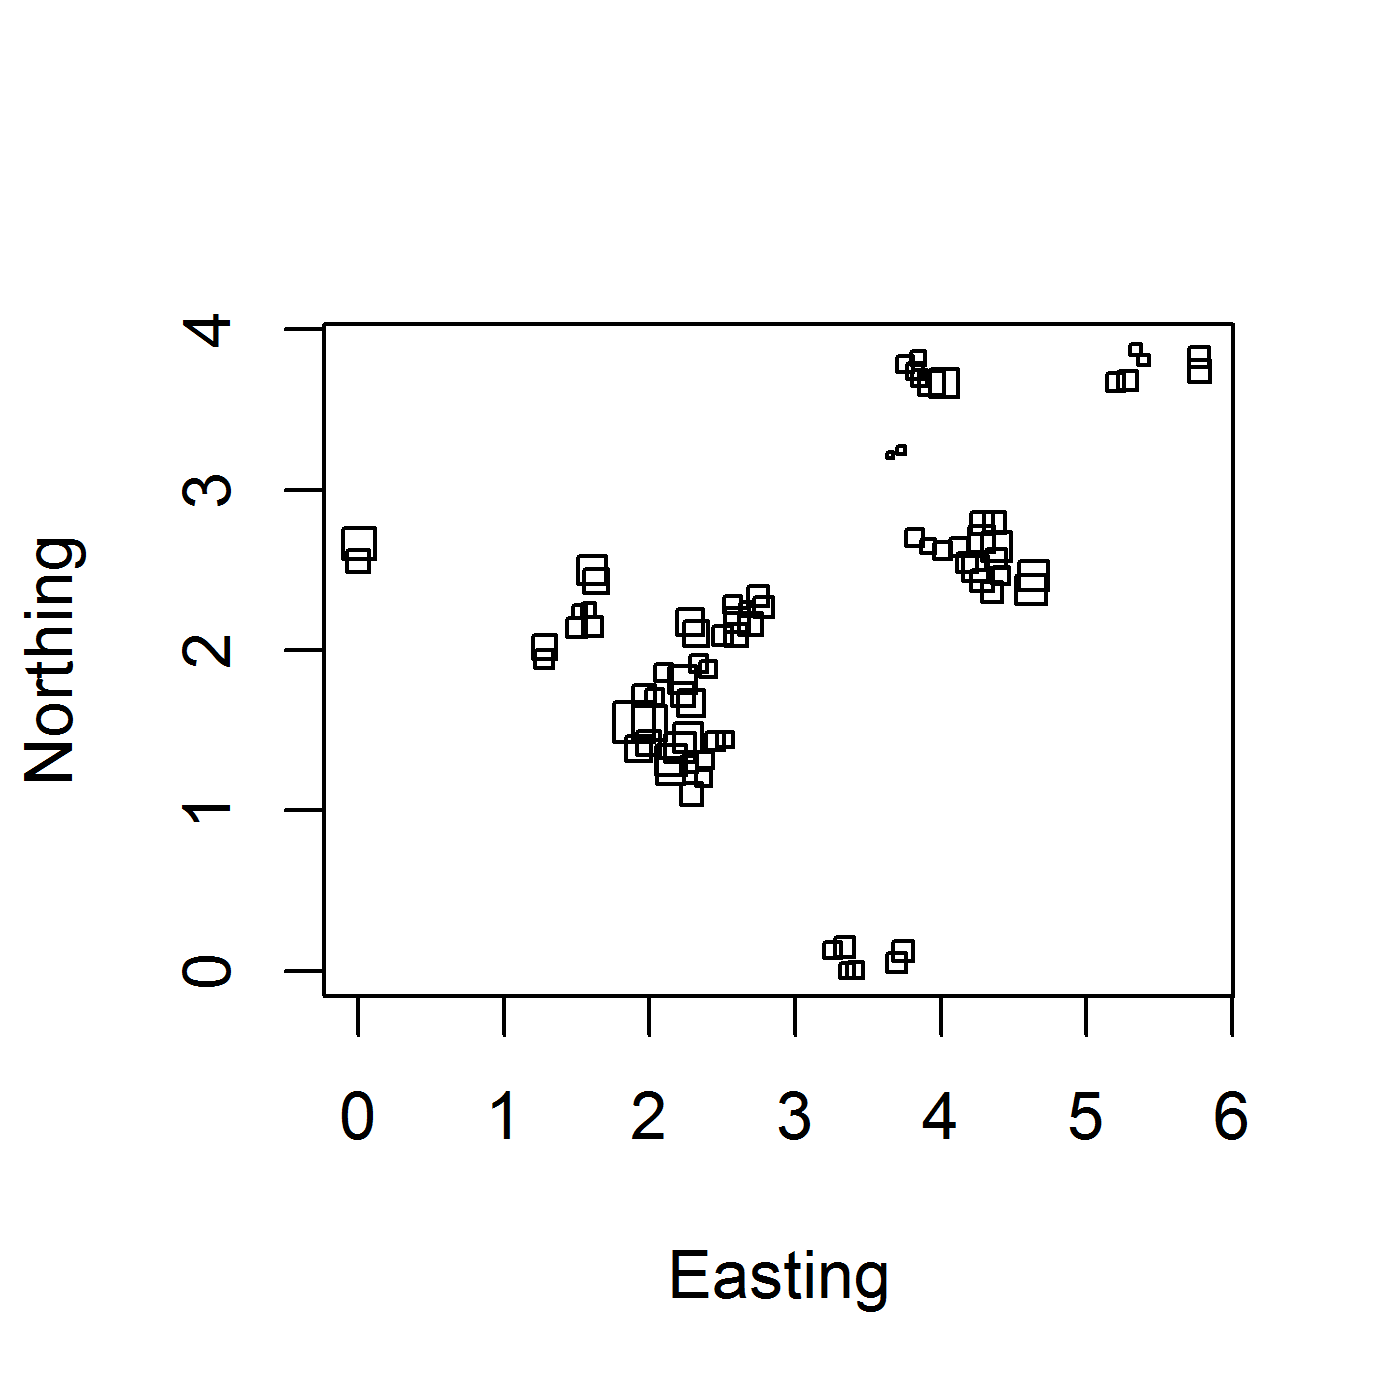
\includegraphics[width=3.5in,height=3.5in]{Ch5/figs/Cap-fragments.png}
\label{poisson-mn.fig.capfrags}
\caption{Relative size and position of 78 forest fragments sampled for
  capricaillie crap.}
\end{figure}


Each of the 44 units
could be sampled by one person in
one day's work (6-8 hours). Within each unit, we focused our search
for droppings on the areas below roosting trees and feeding trees,
respectively, in hiding sites, along internal forest edges, around
root plates and on tree stumps (cf. Jacob et al. 2010). These habitat
elements are the ones preferred by the birds in winter at a small
spatial scale (Bollmann et al. 2005; Mollet unpublished data).
Five spatial units ($I_a$, $S_a$, $S_b$, $H_a$, $T_a$, Table 2) could
not be sampled because of time constraints (too few days with
favorable weather conditions), resulting in 39 units sampled. For the
same reason, three units $(I_b, W_1, W_a)$ were sampled only
once. Access to the area B (Fig. 2) is possible only in late
spring. In 2009, sampling started on 20 April, and the three units in
area B could be sampled only once (rapid snow melting towards the end
of April precluded repetition of sampling here). All other units were
sampled twice.




\subsection{model}

activity centers were uniformly distributed to each of the 78
fragments in proportion to area of the forest patch within which each
fragment was located.


We parameterized activity centers by a discrete state-space with elements
corresponding to the 8 larger fragments. Moreover, home ranges were allocated
to each fragment in  proportion to area. i.e., we assume
define $\lambda_{frag} = A_{frag} \lambda_{0}$, and then:
\[
 N_{frag} \sim Poisson( A_{frag} \lambda_{0} )
\]
This assumption implies the following prior distribution on ${\bf s}_{i}$ (Chapt.
XYZ; Converse and Royle 2012):
\[
{\bf s}_{i} \sim  \mbox{Categorical}(  \pi_{frag} )
\]
with
\[
 \pi_{frag} = \frac{ \lambda_{frag} }{\sum_{frag} \lambda_{frag}}
\]


Observation model:

Each of the 78 fragments is its own sample unit which we index to the
center point of the fragment. No finer scale information is made about
the observation locations.
Let $y_{ij}$ be  the number of times individual $i$ encountered in stand $j$.
Note these are not unique droppings but rather unique clusters of
droppings because a grouse roosting in a tree might leave a number of
droppings and only one of them was sampled\footnote{perhaps this is
  too optimistic of an assessment?}.







\chapter{SCR for Search-Encounter Data with Individual Identity}


\chapter{
MCMC for Spatial Capture-Recapture
}
\markboth{MCMC}{}
\label{chapt.mcmc}

% XXX I kept the R output here because this chapter is about how to look at mcmc output using coda, not so much the actual results
% XXX Need to reconcile the 2 normal Gibbs examples (here and Ch2)


\vspace{.3in}

In this chapter we will dive a little deeper into Markov chain Monte
Carlo (MCMC) sampling. We will construct custom MCMC samplers in {\bf
  R}, starting with easy-to-code GLMs and GLMMs and moving on to
simple CR and SCR models. Finally, we will illustrate some alternative
ready-to-use software packages for MCMC sampling. We will NOT provide
exhaustive background information on the theory and justification of
MCMC sampling -- there are entire books dedicated to that subject and
we refer you to \citet{robert_casella:2004} and
\citet{robert_casella:2010}. Rather we aim to provide you with enough
background and technical know-how to start building your own MCMC
samplers for SCR models in {\bf R}. You will find that quite a few
topics that come up in this chapter have already been covered in
previous chapters, particularly the introduction into Bayesian
analysis in Chapt. \ref{chapt.glms}. To keep you from having to leaf
back and forth we will in some places briefly review aspects of
Bayesian analysis, but we try to focus on the more technical issues of
building MCMC samplers relevant to SCR models.



\subsection{Why build your own MCMC algorithm?}

The standard programs we have used so far to do MCMC analyses are
{\bf WinBUGS} \citep{gilks_etal:1994} and {\bf JAGS}
\citep{plummer:2003}. The wonderful thing about these {\bf BUGS}
engines
is that they automatically use  appropriate and, most of the time, reasonably
efficient forms
of MCMC sampling for the model specified by the user.

The fact that we have such a Swiss Army knife type of MCMC machine
begs the question: Why would anyone want to build their own MCMC
algorithm? For one, there are a limited number of distributions and
functions implemented in {\bf BUGS}. While {\bf OpenBUGS} provides more
options, some more complex models may be impossible to build within
these programs. A very simple example from spatial capture-recapture
that can give you a headache in {\bf WinBUGS} is when your state-space is an
irregular-shaped polygon, rather than an ideal rectangle that can be
characterized by four pairs of coordinates. It is easy to restrict
activity centers to any arbitrary polygon in {\bf R} using an ESRI shapefile
(and we will show you an example in a little bit), but you cannot use
a shape file in a {\bf BUGS} model.  Similarly, models of space usage
that take into account ecological distance
(Chapt. \ref{chapt.ecoldist}) cannot be implemented in the {\bf BUGS}
engines.  Moreover, there are classes of 
SCR models that we have not been able to implement effectively using
likelihood methods, and are inefficient to run in the {\bf BUGS}
engines. Examples are those models covered in Chapts. 
\ref{chapt.scr-unmarked} and \ref{chapt.partialID}. 

Sometimes implementing an MCMC algorithm in {\bf R} may be faster than in
{\bf WinBUGS} - especially if you want to run simulation studies where you
have hundreds or more simulated data sets, several years' worth of
data or other large models, this can be a big advantage.

Finally, building your own MCMC algorithm is a great exercise to
understand how MCMC sampling works. So while using the {\bf BUGS}
language requires you to understand the structure of your model,
building an MCMC algorithm requires you to think about the
relationship between your data, priors and posteriors, and how these
can be efficiently analyzed and characterized. Not to mention that, if
you are an {\bf R} junkie, it can actually be fun.  However, if you
don't think you will ever sit down and write your own MCMC sampler,
consider skipping this chapter - apart from coding it will not cover
anything SCR-related that is not covered by other, more model-oriented
chapters as well.


\section{MCMC and posterior distributions}

MCMC is a class of simulation methods for
drawing (correlated) random numbers from a target distribution, which
in Bayesian inference is the posterior distribution.
As a reminder, the posterior distribution is a probability
distribution for an unknown parameter, say $\theta$, given 
observed data and its prior probability distribution (the probability
distribution we assign to a parameter before we observe data).  The
great benefit of having the posterior distribution of $\theta$ is
that it can be used to make probability statements about $\theta$,
such as the probability that $\theta$ is equal to some value, or the
probability that $\theta$ falls within some range of values. 
The posterior distribution summarizes all we know about a parameter
and thus, is the central object of interest in Bayesian
analysis. Unfortunately, in many if not most practical applications,
it is nearly impossible to directly compute the posterior. Recall
Bayes' theorem:
\begin{equation}
[\theta|y] = \frac{[y|\theta] [\theta]}  {[y]},
\label{mcmc.eq.bayes}
\end{equation}
where $\theta$ is the parameter of interest, $y$ is the observed data,
$[\theta|y]$ is the posterior, $[y|\theta]$ the likelihood of the
data conditional on $\theta$, $[\theta]$ the prior probability of
$\theta$, and, finally, $[y]$ is the marginal probability of the
data, defined as 
\[
[y] = \int [y|\theta]  [\theta] d\theta
\]

This marginal probability is a normalizing constant that ensures that
the posterior integrates to 1. Often, the
integral is difficult or impossible to evaluate, unless you are
dealing with a really simple model.  For example, consider 
a Normal model, with a set of $n$ observations, $y_{i};
i=1,2,\ldots,n$: 
\[
 y_{i} \sim \mbox{Normal}(\mu, \sigma),
\]
where $\sigma$ is known and our objective is to obtain an estimate of
$\mu$. To fully specify the model in a Bayesian
framework, we first have to define a prior distribution for $\mu$. Recall
from Chapt. \ref{chapt.glms} 
that for certain data models, certain priors lead to
conjugacy, i.e. if you choose a certain prior for your parameter,
the posterior distribution will be of a known parametric form. The
conjugate prior for the mean of a Normal model is also a Normal
distribution:
\[
\mu \sim \mbox{Normal}(\mu_0, \sigma_{0}^{2})
\]
If $\mu_{0}$ and $\sigma_{0}^{2}$ are fixed, the posterior for $\mu$
has the following form (for some of the algebra behind this, see Chapt. 2 in \citet{gelman_etal:2004}):
\begin{equation}
\mu|y \sim \mbox{Normal}(\mu_{n}, \sigma_{n}^{2})
\label{mcmc.eq.mu-posterior}
\end{equation}
where
\[
\mu_{n} = \left( \frac{ \sigma^{2}}  {\sigma^{2}   +n \sigma_{0}^{2}} \right) \times  \left(\mu_0 +      \frac{n  \sigma_{0}^{2}}  {\sigma^{2}   +n \sigma_{0}^{2}} \right) \times\bar{y}
\]
And
\[
 \sigma_{n}^{2} = \frac{\sigma^{2}  \sigma_{0}^{2}} {\sigma^{2} + n \sigma_{0}^{2}}
\]
We can directly obtain estimates of interest from this Normal
posterior distribution, such as the mean $\hat{\mu}$ and its variance; we
do not need to apply MCMC, since we can recognize the posterior as a
parametric distribution, including the normalizing constant $[y]$.
But generally we will be interested in more complex models with
several, say $m$, parameters. In this case, computing $[y]$ from
Eq. \ref{mcmc.eq.bayes} requires $m$-dimensional integration, which
can be difficult or impossible. Thus, the posterior distribution in
generally only known up to a constant of proportionality:
\[
[\theta|y] \propto [y|\theta]  [\theta]
\]
The power of MCMC is that it allows us to approximate the posterior
using simulation without evaluating the high dimensional integrals and
to directly sample from the posterior, even when the posterior
distribution is unknown! The price is that MCMC is computationally
expensive. Although MCMC first appeared in the scientific literature
in 1949 \citep{metropolis_etal:1949}, widespread use did not occur
until the 1980s when computational power and speed increased
\citep{gelfand_smith:1990}. It is safe to say that the advent of
practical MCMC methods is the primary reason why Bayesian inference
has become so popular during the past three decades.

In a nutshell, MCMC lets us generate sequential draws of $\theta$ (the
parameter(s) of interest) from distributions approximating the unknown
posterior over $T$ iterations. The distribution of the draw at $t$ depends
on the value drawn at $t$-1; hence, the draws from a Markov
chain\footnote{Remember that for
  $T$ random samples $\theta^ {(1)}$, ... $\theta^{(T)}$ from a Markov chain
  the distribution of $\theta^{(t)}$ depends only on the immediately preceding
  value, $\theta^{(t-1)}$.}. As $T$ goes to infinity, the Markov chain
converges to the desired distribution, in our case the posterior
distribution for $\theta|y$. Thus, once the Markov chain has reached
its stationary distribution, the generated samples can be used to
characterize the posterior distribution, $[\theta|y]$, and point
estimates of $\theta$, its standard error and confidence bounds, can
be obtained directly from this approximation of the posterior. 



\section{Types of MCMC sampling}

There are several general MCMC algorithms in widespread use, the most popular being Gibbs
sampling and Metropolis-Hastings sampling, both of which were briefly
introduced in Chapt. \ref{chapt.glms}. We will be dealing with these
two classes in more detail and use them to construct MCMC
algorithms for SCR models. Also, we will briefly review alternative
techniques that are applicable in some situations.


\subsection{Gibbs sampling}
\label{mcmc.sec.gibbs}

Gibbs sampling was named after the physicist J.W. Gibbs by
\citet{geman_geman:1984}, who applied the algorithm to a Gibbs
distribution\footnote{a distribution from physics we are not going to
  worry about, since it has no immediate connection with Gibbs
  sampling other than giving its name}. The roots of Gibbs sampling
can be traced back to work of \citet{metropolis_ulam:1953}, and it is
actually closely related to Metropolis sampling (see Chapt. 11.5 in
\citet{gelman_etal:2004}, for the link between the two samplers). We
will focus on the technical aspects of this algorithm, but if you find
yourself hungry for more background, \citet{casella_george:1992}
provide a more in-depth introduction to the Gibbs sampler.

Let's go back to our simple example from above to understand the
motivation and functioning of Gibbs sampling. Recall that for a Normal
model with known variance and a Normal prior for $\mu$, the posterior
distribution of $\mu|y$ is also Normal. Conversely, with a fixed
(known) $\mu$, but unknown variance, the conjugate prior for
$\sigma^2$ is an Inverse-Gamma distribution with shape and scale
parameters $a$ and $b$:
\[
\sigma^2 \sim \mbox{Inverse-Gamma}(a,b),
\]
With fixed $a$ and $b$, the posterior $[\sigma^2|\mu,y]$ is also an Inverse-Gamma distribution, namely:
\begin{equation}
\sigma^2|\mu,y \mbox{Inverse-Gamma} (a_n, b_n),
\label{mcmc.eq.sig-posterior}
\end{equation}
 where  $a_n = n/2   + a$ and $b_n = (1/2) \displaystyle\sum\limits_{i=1}^{n} (y_i-\mu)^2 + b$.
However, what if we know neither $\mu$ nor $\sigma^2$, which is probably the
more common case? The joint posterior distribution of $\mu$ and $\sigma^2$
now has the general structure
\[
[\mu, \sigma^2|y] = \frac{[y|\mu,\sigma^2] [\mu] [\sigma^2]}{ \int [y|\mu] [\mu] [\sigma^2] d\mu d\sigma^2 }
\]
or
\[
[\mu, \sigma^2|y] \propto [y|\mu, \sigma^2] [\mu] [\sigma^2]
\]

This cannot easily be reduced to a distribution we recognize. However,
we can condition $\mu$ on $\sigma^2$ (i.e., we treat $\sigma^2$ as fixed) and remove
all terms from the joint posterior distribution that do not involve $\mu$
to construct the full conditional distribution,
\[
[\mu|\sigma^2,y]  \propto [y|\mu] [\mu]
\]

The full conditional of $\mu$ again takes the form of the Normal
distribution shown in Eq. \ref{mcmc.eq.mu-posterior}; similarly, $[\sigma^2|\mu,y]$ takes
the form of the Inverse-Gamma distribution shown in
Eq. \ref{mcmc.eq.sig-posterior}, both distribution we can easily sample
from. And this is precisely what we do when using Gibbs sampling: we
break down high-dimensional problems into convenient one-dimensional
problems by constructing the full conditional distributions for each
model parameter separately; and we sample from these full
conditionals, which, if we choose conjugate priors, are known
parametric distributions.
Let's put the concept of Gibbs sampling into the MCMC framework of
generating successive samples, using our simple Normal model with
unknown $\mu$ and $\sigma^2$ and conjugate priors as an example. These are the
steps you need in order to build a Gibbs sampler:

{\flushleft {\bf Step 0:} Begin with some initial values for $\theta$, say $\theta^{(0)}$.}
In our example, we have to specify initial values for $\mu$ and $\sigma$, for
example by drawing a random number from some Uniform distribution, or
by setting them close to what we think they might be. (Note: This step
is required in any MCMC sampling; chains have to start from
somewhere. We will get back to these technical details a little
later.)
{\flushleft {\bf Step 1:} Draw $\theta^{(1)}$ from the conditional distribution $[\theta_{1}^{(1)}|\theta_{2}^{(0)}$,\ldots, $\theta_{d}^{(0)}]$. }
Here, $\theta_1$ is $\mu$, which we draw from the Normal distribution in Eq. \ref{mcmc.eq.mu-posterior}  using $\sigma^{(0)}$ as value for $\sigma$.
{\flushleft {\bf Step 2:} Draw $\theta_{2}^{(1)}$ from the conditional distribution $[\theta_{2}^{(1)}|\theta_{1}^{(1)}$, $\theta_{3}^{(0)}$,\ldots, $\theta_{d}^{(0)}]$. }
Here, $\theta_2$ is $\sigma$, which we draw from the Inverse-Gamma
distribution of Eq. \ref{mcmc.eq.sig-posterior}, using $\mu^{(1)}$ as value for $\mu$.

{\flushleft {\bf Step 3,\ldots, $d$:} Draw $\theta_{3}^{(1)}$, $\theta_{4}^{(1)}$,\ldots, $\theta_{d}^{(1)}$ from their conditional distribution $[\theta_{3}^{(1)}|\theta_{1}^{(1)}, \theta_{2}^{(1)}, \theta_{4}^{(0)}$, \ldots, $\theta_{d}^{(0)}]$, \ldots, $[\theta_{d}^{(1)}|\theta_{1}^{(1)}$,\ldots, $\theta_{d-1}^{(1)}]$. }
In our example we have no additional parameters, so we only need step 0 through to 2.

{\flushleft {\bf Repeat Steps 1 to $d$} for $T$ = a large number of samples.}

In terms of {\bf R} coding, this means we have to write Gibbs updaters for
$\mu$ and $\sigma^2$ and embed them into a loop over $T$ iterations. The final
code in the form of an {\bf R} function is shown 
in Panel \ref{mcmc.panel.gibbs1}.
\begin{panel}[ht]
\centering
\rule[0.15in]{\textwidth}{.03in}
%\begin{minipage}{2.5in}
{\small
\begin{verbatim}
Norm.Gibbs<-function(y=y,mu_0=mu_0,sigma2_0=sigma2_0,a=a,b=b,niter=niter){

ybar<-mean(y)
n<-length(y)
mu<-1            #mean initial value
sigma2<-1        #sigma2 initial value
an<-n/2 + a      #shape parameter of IvGamma of sigma2

out<-matrix(nrow=niter, ncol=2)
colnames(out)<-c('mu', 'sig')

for (i in 1:niter) {

#update mu according to Eq. 7.2
mu_n<-((sigma2/(sigma2+n*sigma2_0))*mu_0 
+ (n*sigma2_0/(sigma2 + n*sigma2_0))*ybar)
		
sigma2_n <- (sigma2*sigma2_0)/ (sigma2 + n*sigma2_0)
mu<-rnorm(1,mu_n, sqrt(sigma2_n))

#update sigma2 according to Eq. 7.3
bn<- 0.5 * (sum((y-mu)^2)) + b
sigma2<-1/rgamma(1,shape=an, rate=bn)
out[i,]<-c(mu,sqrt(sigma2))

}
return(out)
}
\end{verbatim}
}
%\end{minipage}
\rule[-0.15in]{\textwidth}{.03in}
\caption{
R-code for a Gibbs sampler for a Normal model with unknown $\mu$
and $\sigma$ and conjugate priors (Normal and Inverse-Gamma, respectively) 
for both parameters.
}
\label{mcmc.panel.gibbs1}
\end{panel}

This is it! You can go ahead and simulate some data, $y \sim \mbox{Normal}(5, 0.5)$ and then use the function \mbox{\tt NormGibbs()} in the {\bf R} package \mbox{\tt scrbook} to run your first Gibbs sampler (note that the {\bf R} function {\tt rnorm} requires you to supply the standard deviation $\sigma$ and we have written {\tt NormGibbs} so that it returns $\sigma$ instead of $\sigma^2$ so you can easily compare you input value and parameter estimate). 

\begin{verbatim}
set.seed(13)

#true mean and sd are 5 and 0.5
y<-rnorm(1000, 5,0.5) #data

mu_0<-0 #prior mean
sigma2_0<-100 #prior variance 

#Inverse-Gamma hyperparameters
a<-0.1
b<-0.1 

mod=Norm.Gibbs(y, mu_0, sigma2_0, a,b,niter=10000)
\end{verbatim}

Your output, \verb#mod#, will be a table with two columns, one per
parameter, and $T$ rows, one per iteration. For this 2-parameter example
you can visualize the joint posterior by plotting samples of $\mu$
against samples of $\sigma$ (Fig. \ref{postdist.fig}):
\begin{verbatim}
plot(out[,1], out[,2])
\end{verbatim}
The marginal distribution of each parameter is approximated by
examining the samples of this particular parameter. You can visualize
it by plotting a histogram of the samples (Fig. \ref{plotsofPD.fig} upper left and right):
\begin{verbatim}
par(mfrow=c(1,2))
hist(out[,1]); hist(out[,2])
\end{verbatim}

Finally, recall an important characteristic of Markov chains, namely,
that the chain has to have converged (reached its stationary
distribution) in order to regard samples as coming from the posterior distribution. In
practice, that means you have to throw out some of the initial samples
called the burn-in. We will talk about this in more detail when we talk
about convergence diagnostics. For now, you can use the
\verb#plot(out[,1])# or \verb#plot(out[,2])# command to make a time
series plot of the samples of each parameter and visually assess how
many of the initial samples you should discard. Fig. \ref{plotsofPD.fig} bottom left and right shows
plots for the estimates of $\mu$ and $\sigma$ from our simulated data set;
you see that in this simple example the Markov chain apparently
reaches its stationary distribution very quickly -- the chains look
'grassy' seemingly from the start. It is hard to discern a burn-in
phase visually (but we will see examples further on where the burn-in
is clearer) and you may just discard the first 500 draws to be sure
you only use samples from the posterior distribution. The mean of the
remaining samples are your estimates of $\mu$ and $\sigma$:
\begin{verbatim}
summary(mod[501:10000,])
       mu             sig        
 Min.   :4.935   Min.   :0.4652  
 1st Qu.:4.988   1st Qu.:0.4930  
 Median :4.998   Median :0.5006  
 Mean   :4.998   Mean   :0.5008  
 3rd Qu.:5.009   3rd Qu.:0.5084  
 Max.   :5.062   Max.   :0.5486  
\end{verbatim}

\begin{figure}[ht]
\begin{center}
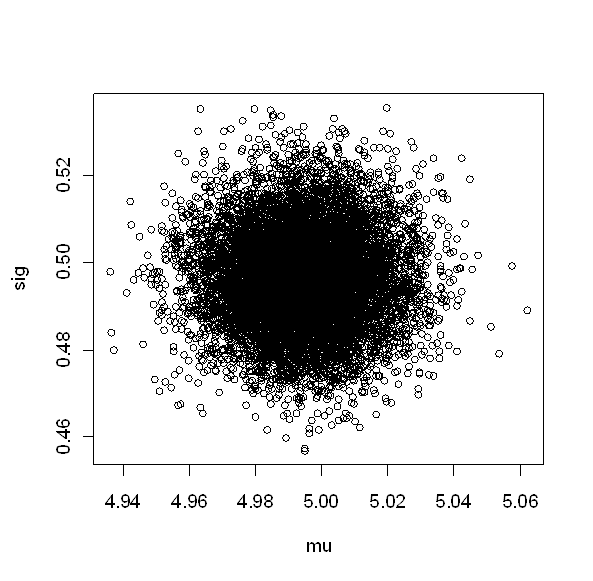
\includegraphics[height=4in]{Ch7/figs/postdist}
\end{center}
\caption{Joint posterior distribution of $\mu$ and $\sigma$ from a Normal Model}
\label{postdist.fig}
\end{figure}

\begin{figure}[ht]
\begin{center}
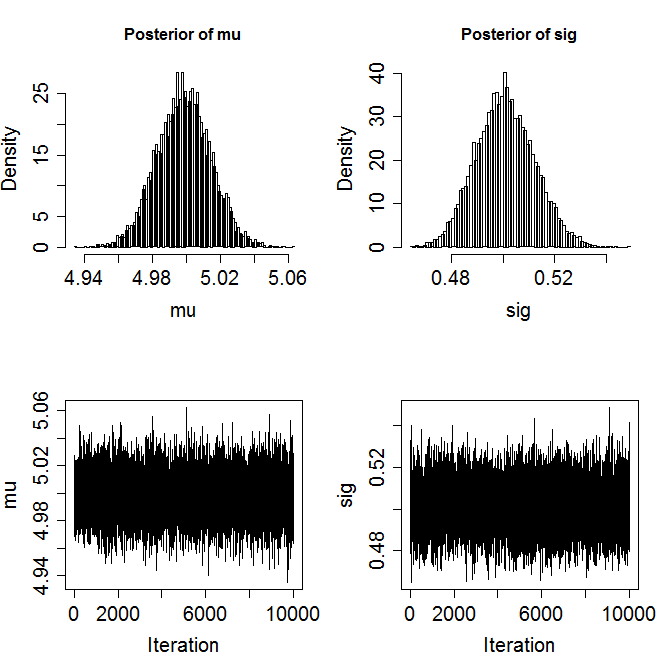
\includegraphics[width=5in]{Ch7/figs/plotsofPD}
\end{center}
\caption{
Plots of the posterior distributions of $\mu$ (upper left) and
  $\sigma$ (upper right)
  from a Normal model and time series plots of $\mu$ (lower left) and $\sigma$ (lower right).}
\label{plotsofPD.fig}
\end{figure}


\subsection{ Metropolis-Hastings sampling   }
\label{mcmc.sec.mh}

Although it is applicable to a wide range of problems, the limitations
of Gibbs sampling are immediately obvious: what if we do not want to
use conjugate priors or what if we cannot recognize the full
conditional distribution as a parametric distribution, or simply do
not want to worry about these issues? The most general solution is to
use the Metropolis-Hastings (MH) algorithm, which also goes back to
the work by \citet{metropolis_ulam:1953}. You saw the basics of this
algorithm in Chapt. \ref{chapt.glms}. In a nutshell, because we do not recognize the
posterior $[\theta|y]$ as a parametric distribution, the MH algorithm
generates samples from a known proposal distribution, say $h(\theta)$,
that depends on the value of $\theta$ at the previous time step,  $\theta^{t-1}$. The candidate value $\theta^*$ is accepted with probability. 

\[
r = \frac{ [\theta^{t-1}|y] h(\theta^{*}|\theta^{t-1})}
    {[\theta^{*}|y] h(\theta^{t}|\theta^{*}) }
\]

Proposal distributions can be absolutely
anything!  You can generate candidate values from a Normal(0,1)
distribution, from a Uniform(-3455,3455) distribution, or anything of
proper support.  Note, however, that good choices of $h()$ are those
that approximate the posterior distribution. Obviously if $h() =
[\theta|y]$ (i.e., the posterior) then you always accept the draw,
and it stands to reason that proposals that are more similar to
$[\theta|y]$ will lead to higher acceptance probabilities. 

The original Metropolis algorithm
required $h(\theta)$ to be symmetric so that
\[
h(\theta^{*}|\theta^{t-1}) = h(\theta^{t-1}|\theta^{*})
\]
In that case these two terms just cancel
out from the MH acceptance probability and $r$ is then just the ratio
of the target density evaluated at the candidate value to that
evaluated at the current value. A later
development of the algorithm by \citet{hastings:1970} lifted this
condition. 
Since using a symmetric proposal distribution makes life a little
easier, we are going to focus on this specific case. A type of symmetric proposal useful in many situations is the
so-called {\it random-walk} proposal distribution where candidate values
are drawn from a normal distribution with mean equal to the current
value and some standard deviation, say $\delta$, which is prescribed by
the user (see below for further explanation). 

{\bf Parameters with bounded support}: Many models contain parameters
that have bounded support. E.g., variance parameters live on
$[0,\infty]$, parameters that represent probabilities live on $[0,1]$,
etc..  For such cases, it is sometimes convenient to use a random walk
proposal distribution that can generate any real number (e.g., a
normal random walk proposal). Under these circumstances you should not
constrain the proposal distribution itself, but you can just reject
parameters that are outside of the parameter space
\citep[sec. 6.4.1 in][]{robert_casella:2010}. You will see plenty of examples of
updating parameters with bounded support in this chapter.

It is worth
knowing that there are alternatives to the random walk MH algorithm. For
example, in the independent MH, $\theta^{*}$ does not depend on
$\theta^{t-1}$, while the Langevin algorithm \citep{roberts_etal:1998}
aims at avoiding the random walk by favoring moves towards regions of
higher posterior probability density. The interested reader should
look up these algorithms in \citet{robert_casella:2004} or
\citet{robert_casella:2010}.

Building a MH sampler can be broken down into several steps. We are going to demonstrate these steps using a different but still simple and common model: the logit-normal or logistic regression model. For simplicity, assume that
\[
y \sim \mbox{Bernoulli} \left(\frac{\exp(\theta)}{1+ \exp(\theta)}\right)
\]
and
\[
\theta \sim \mbox{Normal}(\mu, \sigma)
\]
The following steps are required to set up a random walk MH algorithm:

{\flushleft {\bf Step 0}: Choose initial values, $\theta^{(0)}$.}

{\flushleft {\bf Step 1}: Generate a proposed value of $\theta$ from $h(\theta^{*}|\theta^{t-1})$. }
We often use a Normal proposal distribution, so we draw $\theta^{(1)}$ from $\mbox{Normal}(\theta^{(0)}, \delta)$, where $\delta$ is the variance of the Normal proposal distribution, the tuning parameter that we have to set.

{\flushleft {\bf Step 2}: Calculate the ratio of posterior densities for the proposed and the original value for $\theta$: }
\[
r = \frac{[\theta^{*}|y]}  {[\theta^{t-1}|y]}
\]
In our example,
\[
r = \frac{\mbox{Bernoulli}(y|\theta^{*}) \times \mbox{Normal}(\theta^{*}|\mu, \sigma)} {\mbox{Bernoulli}(y|\theta^{t-1}) \times \mbox{Normal}(\theta^{t-1}|\mu, \sigma)}
\]


{\bf Step 3}: Set
\begin{eqnarray*}
\theta^t  &= &   \theta^{*} \mbox{ with probability min(r,1)}\\
	 & = & 	\theta^{t-1} \mbox{ otherwise }
\end{eqnarray*}

We can do this last step by drawing a random number $u$ from a
$\mbox{Uniform}(0,1)$ and accept $\theta^{*}$ if
$u<r$.
Repeat for $t = 1,2,\ldots$ a large number of samples.
The {\bf R} code for this MH sampler is provided in Panel \ref{mcmc.panel.logitnormal}.

\begin{panel}[ht]
\centering
\rule[0.15in]{\textwidth}{.03in}
%\begin{minipage}{2.5in}
{\small
\begin{verbatim}
Logreg.MH<-function(y=y, mu0=mu0, sig0=sig0, delta=delta, niter=niter) {

out<-c()

theta<-runif(1, -3,3) #initial value

for (iter in 1:niter){
theta.cand<-rnorm(1, theta, delta)

loglike<-sum(dbinom(y, 1, exp(theta)/(1+exp(theta)), log=TRUE))
logprior <- dnorm(theta,mu0 ,sig0, log=TRUE)
loglike.cand<-sum(dbinom(y, 1, exp(theta.cand)/(1+exp(theta.cand)), 
log=TRUE))
logprior.cand <- dnorm(theta.cand, mu0, sig0, log=TRUE)

if (runif(1)<exp((loglike.cand+logprior.cand)-(loglike+logprior))){
theta<-theta.cand
}
out[iter]<-theta
}

return(out)
}
\end{verbatim}
}
%\end{minipage}
\rule[-0.15in]{\textwidth}{.03in}
\caption{
{\bf R} code to run a Metropolis sampler on a simple Logit-Normal model.
}
\label{mcmc.panel.logitnormal}
\end{panel}



The reason we sum the logs of the likelihood and the prior, rather
than multiplying the original values, is simply computational. The
product of small probabilities can be numbers very close to 0, which
computers do not handle well. Thus we add the logarithms, sum, and
exponentiate to achieve the desired result. Similarly, in case you
have forgotten, $x/y = exp(log(x)-log(y))$, with
the latter being favored for computational reasons.

Comparing MH sampling to Gibbs sampling, where all draws from the
conditional distribution are used, in the MH algorithm we discard a
portion of the candidate values, which inherently makes t less
efficient than Gibbs sampling -- the price you pay for its increased
generality.  In Step 1 of the MH sampler we had to choose a variance,
$\delta$, for the Normal proposal distribution. Choice of the
parameters that define our candidate distribution is also referred to
as 'tuning', and it is important since adequate tuning will make your
algorithm more efficient.  $\delta$ should be chosen (a) large enough
so that each step of drawing a new proposal value for $\theta$ can
cover a reasonable distance in the parameter space, as otherwise,
mixing of the Markov chain is inefficient and chains will tend to have
strong autocorrelation; and (b) small enough so that proposal values
are not rejected too often, as otherwise the random walk will 'get
stuck' at specific values for too long.  As a rule of thumb, your
candidate value should be accepted in about 40\% of all
cases. Acceptance rates of 20 -- 80\% are probably ok, but anything
below or above may well render your algorithm inefficient (this does
not mean that it will give you wrong results, only that you will need
more iterations to converge to the posterior distribution). In
practice, tuning will require some 'trial-and-error', some common
sense and, with enough experience, some intuition. Or, one can use an adaptive phase, where the tuning parameter
is automatically adjusted until it reaches a user-defined acceptance
rate, at which point the adaptive phase ends and the actual Markov
chain begins. This is computationally a little more
advanced. \citet{link_barker:2010} discuss this in more detail. It is
important the samples drawn during the adaptive phase are discarded.
To illustrate the effects of tuning, we ran the
Metropolis-within-Gibbs algorithm in Panel \ref{mcmc.panel.logitnormal} with $\delta=0.01$,
$\delta=0.2$ and $\delta=1$. The first 150 iterations for $\theta$ are
shown in Fig. \ref{mcmc.fig.tuning}. We see that for a very small
$\delta$ (the dashed line) the burn-in is extremely slow - after 150
iterations the chain isn't even half way there, while for the other
two values of $\delta$ (solid and dotted) the burn-in phase seems to be
over after only about 10 iterations. While $\delta=0.2$ leads to
reasonably good mixing, the chain clearly gets stuck on certain values
with $\delta=1$.
 \begin{figure}[ht]
\begin{center}
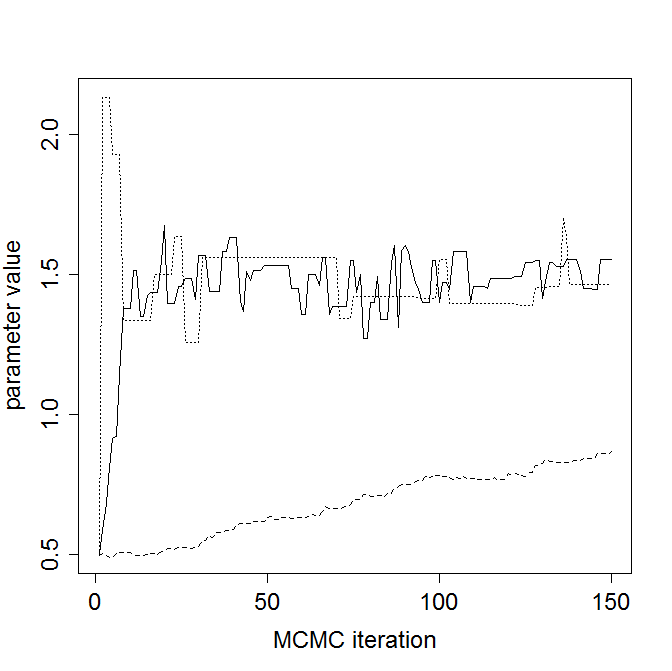
\includegraphics[height=3in,width=3.5in]{Ch7/figs/tuning}
\end{center}
\caption{Time series plots of $\theta$ from a MH algorithm with tuning parameter  $\delta = 0.01$ (dashed line), 0.2 (solid line) and  1 (dotted line).}
\label{mcmc.fig.tuning}
\end{figure}

Other than graphically, you can easily check acceptance rates for the
parameters you monitor (that are part of your output) using the
\verb#rejectionRate()# function of the package {\tt coda} (we will talk more
about this package a little later on). Do not let the term 'rejection
rate' confuse you; it is simply 1 -- acceptance rate. There may be
parameters -- for example, individual values of a random effect or
latent variables -- that you do not want to save, though, and in our
next example we will show you a way to monitor their acceptance rates
with a few extra lines of code.



\subsection{ Metropolis-within-Gibbs }

One weakness of the MH sampler is that formulating the joint posterior
when evaluating whether to accept or reject the candidate values for
$\theta$ becomes increasingly complex or inefficient as the number of
parameters in a model increases. As you already saw in Chapt. \ref{chapt.glms}, in
these cases you can simply combine MH sampling and Gibbs sampling. You
can use Gibbs sampling to break down your high-dimensional parameter
space into easy-to-handle one-dimensional conditional distributions
and use MH sampling for these conditional distributions. Better yet,
if you have some conjugacy in your model, you can use the more
efficient Gibbs sampling for these parameters and one-dimensional MH
for all the others. You have already seen the basics of how to build
both types of algorithms, so we can jump straight into an example here
and build a Metropolis-within-Gibbs algorithm.

{\flushleft \bf  GLMMs: Poisson regression with a random effect }
{\bf XXXX NEED TO FIX MCMC - NOT WORKING RIGHT NOW XXXXXXXXXXXXXXXX} 
Let's assume a model that gets us closer to the problem we ultimately
want to deal with - a GLMM. Here, we assume we have Poisson counts,
$y_{ij}$, from $j=1,2,\ldots,n$ plots in $i$ different study sites,
and we believe that the counts are influenced by some plot-specific
covariate, ${\bf x}$, but that there is also a random site effect. So
our model is:
 
\[
y_{ij} \sim \mbox{Poisson}(\lambda_{ij})
\]
\[
\lambda_{ij} = \exp (\alpha_i + \beta x_{ij})
\]
Let's use Normal priors on $\alpha$ and $\beta$,  \[
\alpha_i \sim \mbox{Normal} (\mu_{\alpha}, \sigma_{\alpha})
\]
and
\[
\beta \sim \mbox{Normal} (\mu_{\beta}, \sigma_{\beta})
\]

In this model, we do not specify $\mu_{\alpha}$ and $\sigma_{\alpha}$, but instead, estimate them as well, so we have
to specify hyperpriors for these parameters:
\begin{eqnarray*}
\mu_{\alpha}  &\sim &  \mbox{Normal}(\mu_0, \sigma_0)  \\
\sigma_{\alpha}^2 & \sim & \mbox{Inverse-Gamma}(a_0, b_0)
\end{eqnarray*}
Note that for simplicity we assume that $\beta$ is constant across the $i$ study sites, and for analysis we would set $\mu_{\beta}$ and $\sigma_{\beta}$.
With the model completely specified, we can compile the full conditionals,
breaking the multi-dimensional parameter space into one-dimensional
components:

\begin{eqnarray*}
[\alpha_1|\alpha_2,\alpha_3,\ldots,\alpha_i,\beta,{\bf y}_{1}] & \propto &   [{\bf y}_{1}|\alpha_1,\beta]  [\alpha_1] \\
	 & \propto  &   \mbox{Poisson}({\bf y}_{1}| \exp(\alpha_1 + \beta {\bf x}_1)) \times \mbox{Normal}(\alpha_1|\mu_{\alpha} , \sigma_{\alpha})
\end{eqnarray*}
where ${\bf y}_{1} = (y_{11},y_{12}, \ldots, y_{1n})$ is the vector of
observed counts for site $i=1$ and, in general, ${\bf y}_{i}$ is the
vector of all counts for site $i$; analogous, ${\bf x}_{i}$ is the
vector of all observations of the covariate for site $i$. The other full conditionals for
each $\alpha_{i}$ are constructed similarly:

\begin{eqnarray*}
[\alpha_2|\alpha_1,\alpha_3,\ldots,\alpha_i,\beta,{\bf y}_{2}] & \propto&  [{\bf y}_{2}|\alpha_2,\beta]  [\alpha_2] \\
	 & \propto  & \mbox{Poisson}({\bf y}_{2}| \exp(\alpha_2 + \beta {\bf x}_2)) \times \mbox{Norm}(\alpha_2|\mu_{\alpha}, \sigma_{\alpha})
\end{eqnarray*}
and so on for all elements of ${\bf \alpha}$. The full-conditional for $\beta$ is:
\begin{eqnarray*}
[\beta|{\bf \alpha},{\bf y}] &\propto & [{\bf y}|{\bf \alpha},\beta]  [\beta] \\
	 &\propto& \mbox{Poisson}({\bf y}|exp({\bf \alpha} + \beta {\bf x})) \times \mbox{Normal}(\beta|\mu_{\beta}, \sigma_{\beta})
\end{eqnarray*}

Finally, we need to update the hyperparameters for the random effects
vector ${\bf \alpha}$:
\[
[\mu_{\alpha}|{\bf \alpha}] \propto [{\bf \alpha}|\mu_{\alpha}, \sigma_{\alpha}] [\mu_{\alpha}]
\]
\[
[\sigma_{\alpha}|{\bf\alpha}] \propto [{\bf \alpha}|\mu_{\alpha}, \sigma_{\alpha}] [\sigma_{\alpha}]
\]
Since we assumed ${\bf \alpha}$ to come from a Normal distribution,
the choice of priors for $\mu_{\alpha}$ (Normal) and $\sigma_{\alpha}^2$
(Inverse-Gamma) leads to the same conjugacy we observed in our initial
Normal model, so that both hyperparameters can be updated using Gibbs
sampling.

Now let's build the updating steps for these full conditionals. Again,
for the MH steps that update ${\bf \alpha}$ and $\beta$ we use Normal
proposal distributions with standard deviations $\delta_{\alpha}$ and
$\delta_{\beta}$.

First, we set the initial values ${\bf \alpha}^{(0)}$ and
$\beta^{(0)}$. Then, starting with $\alpha_1$, we draw
$\alpha_1^{(1)}$ from $\mbox{Norm}(\alpha_1^{(0)}, \delta_{\alpha})$,
calculate the conditional posterior density of $\alpha_1^{(0)}$ and
$\alpha_1^{(1)}$ and compare their ratios,
\[
r = \frac{\mbox{Poisson}({\bf y}_{1}|exp(\alpha_1^{(1)} + \beta {\bf x}_1)) \times
  \mbox{Normal}(\alpha_1^{(1)}|\mu_{\alpha}, \sigma_{\alpha})} {\mbox{Poisson}({\bf y}_{1}|exp(\alpha_1^{(0)} + \beta {\bf x}_1)) \times \mbox{Normal}(\alpha_1^{(0)}|\mu_{\alpha}, \sigma_{\alpha})}
\]
and accept $\alpha_1^{(1)}$ with probability $min(r,1)$. We repeat this for all ${\bf \alpha}$.

For $\beta$, we draw $\beta^{(1)}$ from $\mbox{Norm} (\beta^{(0)}, \delta_{\beta})$, compare the posterior densities of $\beta^{(0)}$ and $\beta^{(1)}$,
\[
r = \frac{\mbox{Poisson}({\bf y}|exp({\bf \alpha} + \beta^{(1)}{\bf x}))
  \times\mbox{Normal}(\beta^{(1)}|\mu_{\beta}, \sigma_{\beta})} { \mbox{Poisson}({\bf
    y}|exp({\bf \alpha} + \beta^{(0)}{\bf x})) \times \mbox{Normal}(\beta^{(0)}|\mu_{\beta}, \sigma_{\beta})},
\]
and accept $\beta^{(1)}$  with probability $min(r,1)$.

For $\mu_{\alpha}$ and $\sigma_{\alpha}^2$, we sample directly from the full conditional distributions (Eq. \ref{mcmc.eq.mu-posterior}  and Eq. \ref{mcmc.eq.sig-posterior}):
\[
\mu_{\alpha}^{(1)} \sim \mbox{Norm} (\mu_n, \sigma_n^2)
\]
where 
\[\mu_n =  \frac{\sigma_{\alpha}^{2(0)}}  {\sigma_{\alpha}^{2(0)}   +n_{\alpha}    \sigma_0^2} \times  \mu_0 +  \frac{n_{\alpha}  \sigma_0^2} {\sigma_{\alpha}^{2(0)}   +n_{\alpha} \sigma_0^2} \times \bar{\alpha}^{(1)}
\]
and 
\[
\sigma_n^2= \frac{\sigma_{\alpha}^{2(0)}   \sigma_0 } {\sigma_{\alpha}^{2(0)}  + n \sigma_0^2}
\]
Here, $\bar{\alpha}$ is the current mean of the vector ${\bf\alpha}$, which we
updated before, and $n_{\alpha}$ is the length of ${\bf\alpha}$. 
For $\sigma_{\alpha}^2$ we use $\sigma_{\alpha}^{2(1)}\sim \mbox{Inverse-Gamma} (a_n, b_n)$,
where  $a_n = n_a/2   + a_0$, and $b_n = 0.5  \displaystyle\sum\limits_{i=1}^{n_{\alpha}} (\alpha_i^{(1)}-\mu_{\alpha}^{(1)})^2+ b_0$.


We repeat these steps over $T$ iterations of the MCMC algorithm. Call
the function \mbox{\tt PoisGLMM()} in \mbox{\tt scrbook} to check out
what this algorithm looks like in {\bf R}.

In this example we may not want to save each individual $\alpha$, but
are only interested in their mean and standard deviation. Since these
two parameters will change as soon as the value for one element in
$\bf{\alpha}$ changes, their acceptance rates will always be close to
1 and are not representative of how well your algorithm performs. To
monitor the acceptance rates of parameters you do not want to save,
you simply need to add a few lines of code into your updater to see
how often the individual parameters are accepted. The code for
updating {\bf $\alpha$} from our Poisson GLMM below shows one way how to
monitor acceptance of individual $\alpha$'s.

{\small
\begin{verbatim}
#initiate counter for acceptance rate of alpha
alphaUps<-0

#loop over sites, update intercepts alpha one at a time; 
#only data at site i contributes information			
#lev is the number of sites i
for (i in 1:lev) { 		
alpha.cand<-rnorm(1, alpha[i], delta_alpha)	
loglike<- sum(dpois (y[site==i], exp(alpha[i] + beta*x[site==i]), 
		  log=TRUE))  
logprior<- dnorm(alpha[i], mu_alpha,sig_alpha, log=TRUE)
loglike.cand<- sum(dpois (y[site==i], exp(alpha.cand + beta *x[site==i]), 
			   log=TRUE))
logprior.cand<- dnorm(alpha.cand,  mu_alpha,sig_alpha, log=TRUE)
if (runif(1)< exp((loglike.cand+logprior.cand) -(loglike+logprior))) {
alpha[i]<-alpha.cand
alphaUps<-alphaUps+1
}
}

#lets you check the acceptance rate of alpha at every 100th iteration
if(iter %% 100 == 0) {  
            cat("   Acceptance rates\n")
            cat("     alpha =", alphaUps/lev, "\n")
}
\end{verbatim}
}

\subsection{Rejection sampling and slice sampling }

While MH and Gibbs sampling are probably the most widely applied
algorithms for posterior approximation, there are other options that
work under certain circumstances and may be more efficient when
applicable. {\bf WinBUGS} applies these algorithms and we want you to be
aware that there is more out there to approximate posterior
distributions than Gibbs and MH.  One alternative algorithm is
rejection sampling. Rejection sampling is not an MCMC method, since
each draw is independent of the others. The method can be used when
the posterior $[\theta|y]$ is not a known parametric distribution but
can be expressed in closed form. Then, we can use a so-called envelope
function, say, $g(\theta)$, that we can easily sample from, with the
restriction that $[\theta|y] < M \times g(\theta)$. We then sample a
candidate value for $\theta$ from $g(\theta)$, calculate $r =
[\theta|y]/M \times g(\theta)$ and keep the sample with the probability
$r$. $M$ is a constant that has to be picked so that $r$ lies between
0 and 1, for example by evaluating both $[\theta|y]$ and $g(\theta)$
at $n$ points and looking at their ratios. Rejection sampling only
works well if $g(\theta)$ is similar to $[\theta|y]$, and packages
like {\bf WinBUGS} use adaptive rejection sampling \citep{gilks_wild:1992},
where a complex algorithm is used to fit an adequate and efficient
$g(\theta)$ based on the first few draws. 
Though efficient in some
situations, rejection sampling does not work well with
high-dimensional problems, since it becomes increasingly hard to
define a reasonable envelope function. For an example of rejection
sampling in the context of SCR models, see
Chapt. \ref{chapt.state-space}, where we use it to simulation
non-stationary point processes.  

Another alternative is slice sampling
\citep{neal:2003}. In slice sampling, we sample uniformly from the
area under the plot of $[\theta|y]$. Considering a single univariate
$\theta$. Let's define an auxiliary variable, $U \sim \mbox{Unif}(0,
[\theta|y])$. Then, $\theta$ can be sampled from the vertical slice
of $[\theta|y]$ at $U$ (Fig. \ref{mcmc.fig.slicesample}):
\[
\theta|U \sim \mbox{Unif}(B),
\]
where $B = \{\theta: [\theta|y] \geq U\}$

\begin{figure}[ht]
\begin{center}
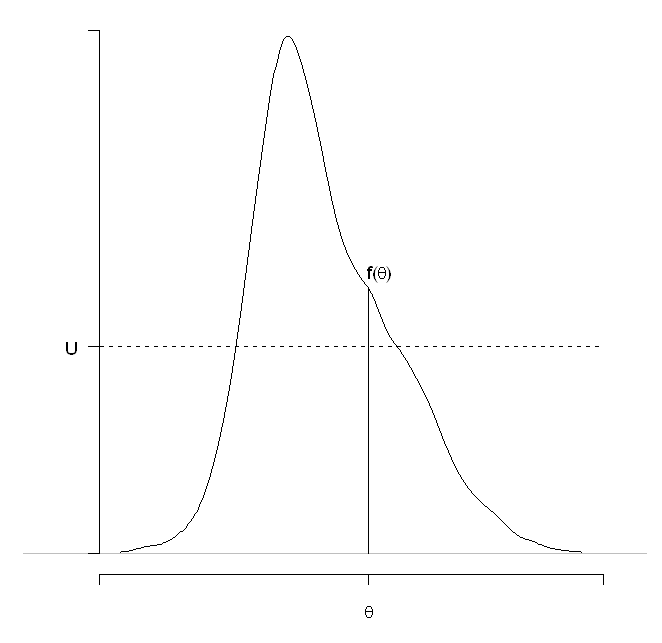
\includegraphics[height=3in]{Ch7/figs/slicesampling}
\end{center}
\caption{
Slice sampling. For 
$U \sim \mbox{Unif}(0, [\theta|y])$, 
we can sample $\theta$ from the vertical slice of $[\theta|y]$ at $U$; 
$\theta|U \sim \mbox{Unif}(B)$, 
where $B = \{ \theta: [\theta|y] \geq U\}$.
}
\label{mcmc.fig.slicesample}
\end{figure}

%Slice sampling. For $U \sim \mbox{Unif} (0, [\theta|y])$, we can sample $\theta$ from the vertical slice of $[\theta|y]$ at $U$;  $theta|U \sim \mbox{Unif}(B)$, where $B = {\theta: [\theta|y] \geq U\}$.

Slice sampling can be applied in many situations; however,
implementing an efficient slice sampling procedure can be
complicated. We refer the interested reader to 
\citet[][Chapt. 7]{robert_casella:2010} for a simple example.  Both rejection
sampling and slice sampling can be applied on one-dimensional
conditional distributions within a Gibbs sampling setup.

\section{MCMC for closed capture-recapture Model Mh}

By now you have seen MCMC samplers for some simple GL(M)M's. Now, to
ease you into more complex models, we construct our own MCMC algorithm
using a Metropolis-within-Gibbs sampler for the non-spatial model with
individual heterogeneity in capture probability, model $M_{h}$, developed in
Chapt. \ref{chapt.closed}.

To recapitulate: Under the non-spatial model, each of the $n$ observed
individuals is either detected (1) or not (0) during each of $K$
sampling occasions. We estimate $N$ using data augmentation and have a
Bernoulli model for the data augmentation variables $z_{i}$. 
\[
z_{i} \sim \mbox{Bernoulli}(\psi)
\]
The binomial
observation model is expressed conditional on the latent variables
$z_{i}$. 
\[
y_i \sim \mbox{Binomial} (p_i \times z_i, K)
\]
Further, we prescribe a distribution for the capture
probability $p_{i}$. Here we assume
\[
\mathrm{logit}(p_{i}) \sim \mbox{Normal}(\mu,\sigma^2)
\]

As usual, we have to go through two general steps before we write the MCMC algorithm:
\begin{itemize}
\item[  (1)] Identify the model with all its components (including
    priors)
\item[  (2)] Recognize and express the full conditional distributions for
    all parameters
\end{itemize}
Our model components are as follows: $[y_{i}| p_{i},z_{i}]$,
$[p_{i}|\mu_{p},\sigma_{p}]$, and $[z_{i}|\psi]$
for {\it each} $i=1,2,\ldots,M$ and then prior distributions
$[\mu_{p}]$, $[\sigma_{p}]$ and $[\psi]$.
The joint posterior distribution of all unknown quantities in the model
is proportional to the joint distribution of all elements
$y_{i},p_{i},z_{i}$ and also the prior distributions of the prior parameters:
\[
\left\{ \prod_{i=1}^{M} [y_{i}|p_{i},z_{i}][p_{i}|\mu_{p},\sigma_{p}]
[z_{i}|\psi] \right\} [\mu_{p},\sigma_{p},\psi]
\]
For prior distributions, we assume that $\mu_{p},\sigma_{p}, \psi$ are
mutually independent and for $\mu_{p}$ and $\sigma_{p}$ we use
improper uniform priors, and $\psi \sim \mbox{Unif}(0,1)$.  This is
equivalent to $\mbox{Beta}(1,1)$, which will come in handy, as we will
see in a moment. Note that the likelihood contribution for each
individual, when conditioned on $p_{i}$ and $z_{i}$, does not depend
on $\psi$, $\mu_{p}$, or $\sigma_{p}$.  As such, the full-conditional
for the structural parameter $\psi$ only depend on the collection of
data augmentation variables $z_{i}$, and that for $\mu_{p}$ and
$\sigma_{p}$ will only depend on the collection of latent variables
$p_{i}; i=1,2,\ldots,M$.  The full conditionals for all the unknowns
are as follows:

{\bf (1)} For $p_{i}$:
\begin{eqnarray*}
[p_{i}|y_{i}, \mu_p, \sigma_{p},z_{i}] &\propto  &
[y_{i}|p_{i}][p_{i}|\mu_p,\sigma_{p}^{2}] \mbox{ if $z_{i}=1$ }  \\
                 &  &  [p_{i}|\mu_p,\sigma_{p}] \mbox{ if $z_{i}=0$ }
\end{eqnarray*}

{\bf (2)} for $z_{i}$:
\[
[z_{i} | y_{i}, p_{i}, \psi] \propto [y_{i}|z_{i} \times p_{i}] \mbox{Bernoulli}(z_{i}|\psi)
\]

{\bf (3)} For $\mu_{p}$:
\[
[\mu_{p} | p_{i}, \sigma_{p}] \sim \left\{ \prod_{i} [p_{i}|\mu_{p}, \sigma_{p}] \right\} \times \mbox{const}
\]

{\bf (4)} For $\sigma_{p}$:
\[
[ \sigma_{p}|p_{i}, \mu_{p} ] \sim \left\{ \prod_{i}[p_{i}| \mu_{p},\sigma_{p} ] \right\} \times \mbox{const}
\]

{\bf (5)} For $\psi$:
\[
[\psi|z_{i}] \propto \left\{ \prod_{i} [z_{i}|\psi] \right\} \mbox{Beta}(1,1)
\]
Remember that \mbox{Beta}(1,1) is equivalent to \mbox{Uniform}(0,1). The beta distribution is the conjugate prior to the binomial and 
Bernoulli distributions and the general form of a full conditional of a beta-binomial model 
with $x_{i} \sim \mbox{Bernoulli} (p) $ and $p \sim \mbox{Beta}(a,b)$ is
\[
[p|{\bf x}] \propto \mbox{Beta}(a + \sum_i x_i, b + n-\sum_i x_i)
\]
In our case that means
\[
[\psi|z_{i}] \propto \mbox{Beta}(1 + \sum z_{i}, 1 + M - \sum z_{i})
\]

What we've done here is identify each of the full conditional
distributions in sufficient detail to toss them into our
Metropolis-Hastings algorithm (the constant term in the full
conditionals for $\mu_{p}$ and $\sigma_{p}$ reflects the improper
prior we chose for both parameters).  Below, you see the updating step
for the detection parameter ${\bf p}$. Note that (1) we draw candidate
values on the logit scale and (2) instead of looping through $1 - M$
individuals to update all $p_{i}$, we update all elements of the
vector of {\bf p} in parallel.

\begin{verbatim}
### update the logit(p) parameters
lp.cand<- rnorm(M,lp,1)  # 1 is a tuning parameter
p.cand<-plogis(lp.cand)
ll<-dbinom(ytot,K,z*p, log=T)
prior<-dnorm(lp,mu,sigma, log=T)
llcand<-dbinom(ytot,K,z*p.cand, log=T)
prior.cand<-dnorm(lp.cand,mu,sigma, log=T)

kp<- runif(M) < exp((llcand+prior.cand)-(ll+prior))
p[kp]<-p.cand[kp]
lp[kp]<-lp.cand[kp]
\end{verbatim}

The parameters $\mu_{p}$ and $\sigma_{p}$ are also updated using MH steps (see the code for $\mu_{p}$ below). In truth, we could also sample $\mu_{p}$
and $\sigma_{p}^{2}$ directly with certain choices of prior
distributions. For example, if $\mu_{p} \sim \mbox{Normal}(0, 1000)$
then the full conditional for $\mu_{p}$ is also Normal (see
sec. \ref{mcmc.sec.gibbs}), etc..

\begin{verbatim}
p0.cand<- rnorm(1,p0,.05)
if(p0.cand>0 & p0.cand<1){
mu.cand<-log(p0.cand/(1-p0.cand))
ll<-sum(dnorm(lp,mu,sigma,log=TRUE))
llcand<-sum(dnorm(lp,mu.cand,sigma,log=TRUE))
if(runif(1)<exp(llcand-ll)) {
 mu<-mu.cand
 p0<-p0.cand
}
}
\end{verbatim}

For $\psi$ we can easily sample directly from the beta distribution:

\begin{verbatim}
psi<-rbeta(1, sum(z) + 1, M-sum(z) + 1)
\end{verbatim}

To update the $z_{i}$ we have opted for a MH updater 
(although they could be updated directly from their
full-conditional). Since $z_{i}$ can only take the values of 0 or 1, we generate candidate values using \verb#z.cand<-ifelse(z==1,0,1)#.
You can check out the full code by invoking \mbox{\tt modelMh()} from the {\bf R} package \mbox{\tt scrbook}.

\section{MCMC algorithm for model SCR0}

Conceptually, but also in terms of MCMC coding, it is only a small
step from the non-spatial model $M_h$ to a fully spatial
capture-recapture model. Next, we'll walk you through the steps of
building your own MCMC sampler for the basic SCR model (i.e. without
any individual, site or time specific covariates) with both a Poisson
and a Binomial encounter process.  As usual, we will have to go
through two general steps before we write the MCMC algorithm:
\begin{itemize}
\item[  (1)] Identify the model with all its components (including
    priors)
\item[  (2)] Recognize and express the full conditional distributions for
    all parameters
\end{itemize}
It is worthwhile to go through all of step 1 for an SCR model, but you
have probably seen enough of step 2 in our previous examples to get
the essence of how to express a full conditional
distribution. Therefore, we will exemplify step 2 for some parameters
and tie these examples directly to the respective R code.

{\bf Step 1 -- Identify your model}

Recall the components of the basic SCR model with a Poisson encounter process from Chapt. \ref{chapt.poisson-mn}:
We assume that individuals $i$, or rather, their activity centers
${\bf s}_i$, are uniformly distributed across the state space ${\cal S}$,
\[
{\bf s}_i  \sim \mbox{Uniform}({\cal S})
\]
and that the number of times individual $i$ encounters trap $j$, $y_{ij}$, is a Poisson variable with mean $\lambda_{ij}$,
\[
y_{ij} \sim \mbox{Poisson}(\lambda_{ij})
\]
The link between individual location, movement and trap encounter
rates is made by the assumption that $\lambda_{ij}$, is a decreasing
function of the distance between ${\bf s}_i$ and the location of $j$,
${\bf x}_{j}$, say $d_{ij} = ||{\bf s}_{i} - {\bf x}_{j}||$, of the half-normal form
\[
\lambda_{ij} =  \lambda_0  \exp(-d_{ij}^2/2\sigma^2),
\]
where $\lambda_0$ is the baseline trap encounter rate at $d_{ij}=0$ and $\sigma$ controls the shape of the half-normal function.

In order to estimate the number of ${\bf s}_i$ in ${\cal S}$ (or any
subset of ${\cal S}$), $N$, we use data augmentation (sec. \ref{closed.sec.da}) and create $M-n$ all-zero encounter histories, where $n$ is the number of individuals we observed and $M$ is a somewhat arbitrary number that is larger than $N$. We estimate $N$ by summing over the auxiliary data augmentation variables, $z_i$, which is 1 if the individual is part of the population and 0 if not, and assume that $z_i$ is a Bernoulli random variable,
\[
z_{i} \sim \mbox{Bernoulli}(\psi)
\]

To link the two model components, we modify our trap encounter model to
\[
\lambda_{ij} = \lambda_0 \times \exp(-d_{ij}^2/2\sigma^2) \times z_{i}.
\]
The model has the following structural parameters, for which we need to specify priors:
\begin{itemize}
\item[ $\psi$:] the $\mbox{Uniform}(0,1)$ is required as part of the data augmentation procedure and in general is a natural choice of an uninformative prior for a probability. It will also lead to conjugacy as we saw in the example of model $M_h$, so that we can update $\psi$ directly from its full conditional distribution using Gibbs sampling.
\item[ ${\bf s}_{i}$:] since ${\bf s}_{i}$ is a pair of coordinates it is two-dimensional and we use a uniform prior limited by the extent of our state-space over both dimensions.
\item[ $\sigma$:] we can conceive several priors for $\sigma$ but let's assume an improper prior, one that is Uniform over $(-\infty, \infty)$. We will see why this is convenient when we construct the full conditionals for $\sigma$.
\item[ $\lambda_{0}$:] analogous, we will use a $\mbox{Uniform}(-\infty, \infty)$ improper prior for $\lambda_{0}$.
\end{itemize}
The parameter that is the objective of our modeling, $N$, is a derived parameter that we can obtain by summing all $z_i$:
\[
N = \sum_{i=1}^{M} z_{i}
\]

{\bf Step 2 -- Construct the full conditionals:}
Having completed step 1, let's look at the full conditional distributions for some of these parameters.
We find that with improper priors, full conditionals are proportional only to the likelihood of the observations; for example, consider $\sigma$:
\[
[\sigma|{\bf s}, \lambda_{0}, {\bf z}, {\bf y}] \propto \left\{ \prod_{i} [y_{i}| {\bf
    s}_{i}, \lambda_{0}, z_{i}, \sigma] \right\}  [\sigma]
\]
Since the improper prior implies that $[\sigma] \propto 1$, we can reduce this further to
\[
[\sigma|{\bf s}, \lambda_{0}, {\bf z}, {\bf y}] \propto \left\{
  \prod_{i} [y_{i}| {\bf s}_{i}, \lambda_{0}, z_{i}, \sigma] \right\}
\]
The {\bf R} code to update $\sigma$ is shown below.
Notice that we automatically reject negative candidate values, since $\sigma$ cannot be $<0$.  

\begin{verbatim}
sig.cand <- rnorm(1, sigma, 0.1)	#draw candidate value
 if(sig.cand>0){   #automatically reject sig.cand that are <0
     lam.cand <- lam0*exp(-(d*d)/(2*sig.cand*sig.cand))
     ll<- sum(dpois(y, lam*z, log=TRUE))
     llcand <- sum(dpois(y, lam.cand*z, log=TRUE))
     if(runif(1) < exp( llcand  - ll) ){
         ll<-llcand
         lam<-lam.cand
         sigma<-sig.cand
      }
  }
\end{verbatim}

These steps are analogous for  $\lambda_{0}$ and ${\bf s}_i$ and we will 
use MH steps for
all of these parameters. Similar to the random intercepts in our
Poisson GLMM, we update each ${\bf s}_i$ individually. Note that to be fully
correct, the full conditional for ${\bf s}_i$ contains both the likelihood and
prior component, since we did not specify an improper, but a proper Uniform
prior on ${\bf s}_i$. However, with a Uniform distribution the probability
density of any value is 1/(upper limit - lower limit) =
constant. Thus, the prior components are identical for both the
current and the candidate value and can be ignored (formally, when you
calculate the ratio of posterior densities, $r$, the identical prior
component appears both in the numerator and denominator, so that they
cancel each other out).

We still have to update $z_i$. The full conditional for $z_i$ is
\[
[z_i|y_{i}, \sigma, \lambda_0, {\bf s}_{i}] \propto [y_{i}|z_{i},\sigma, \lambda_0, 
{\bf s}_{i}] [z_i]
\]
and since $z_i \sim \mbox{Bern}(\psi)$,
the term has to be taken into account when updating $z_i$:

\begin{verbatim}
        zUps <- 0		#set counter to monitor acceptance rate
        for(i in 1:M) {
        #no need to update seen individuals, since their z =1
            if(seen[i])	
                next
            zcand <- ifelse(z[i]==0, 1, 0)
            llz <- sum(dpois(y[i,],lam[i,]*z[i], log=TRUE))
            llcand <- sum(dpois(y[i,], lam[i,]*zcand, log=TRUE))

            prior <- dbinom(z[i], 1, psi, log=TRUE)
            prior.cand <- dbinom(zcand, 1, psi, log=TRUE)
            if(runif(1) < exp((llcand+prior.cand)-(llz+prior))){
                z[i] <- zcand
                zUps <- zUps+1
            }
        }
\end{verbatim}
The parameter $\psi$ is a hyperparameter of the model, with an uninformative prior 
 distribution of $\mbox{Uniform}(0,1)$ or $\mbox{Beta}(1,1)$, so that
\[
[\psi|{\bf z}] \propto \mbox{Beta}(1 + \sum_i z_i, 1 + M-\sum_i z_i)
\]


These are all the building blocks you need to write the MCMC algorithm
for the spatial null model with a Poisson encounter process.  You can
find the full {\bf R} code by calling the function (\mbox{\tt SCR0pois}) in the {\bf R} package 
\mbox{\tt scrbook}.

\subsection{SCR model with binomial encounter process}
The equivalent SCR model with a binomial encounter process is very
similar. Here, each individual $i$ can only be detected once at any
given trap $j$ during a sampling occasion $k$.  Thus
\[
y_{ij} \sim \mbox{Binomial} (p_{ij}, K)
\]
Where $p_{ij}$ is some function of distance between ${\bf s}_{i}$ and trap location ${\bf x}_{j}$. Here we use:
\[
p_{ij}=1-\mbox{exp}(-\lambda_{ij})
\]
Recall from Chapt. \ref{chapt.glms} that this is the complementary log-log (cloglog) link function, which constrains $p_{ij}$ 
to fall between 0 and 1.
For our MCMC algorithm that means that, instead of using a Poisson 
likelihood, $\mbox{Poisson}(y|\sigma,\lambda_0,{\bf s},z)$, we use a 
Binomial likelihood, $\mbox{Binomial}(y| \sigma,\lambda_0,{\bf s},z; K)$, 
in all the conditional distributions. An exemplary updating step for $\lambda_0$ under a Binomial encounter model is shown below. 
The full MCMC code for the Binomial SCR with a clog-log link (\mbox{\tt SCR0binom.cl}) 
can be found in the {\bf R} package \mbox{\tt scrbook}.

\begin{verbatim}
        lam0.cand <- rnorm(1, lam0, 0.1)
        #automatically reject lam0.cand that are <0
        if(lam0.cand >0){   
            lam.cand <- lam0.cand*exp(-(d*d)/(2*sigma*sigma))
            p.cand <- 1-exp(-lam.cand)
            ll<- sum(dbinom(y, K, pmat *z, log=TRUE))  
            llcand <- sum(dbinom(y, K, p.cand *z, log=TRUE))
            if(runif(1) < exp( llcand  - ll) ){
                ll<-llcand
                pmat<-p.cand
                lam0<- lam0.cand
            }
        }
\end{verbatim}

Another possibility is to model variation in the individual and site 
specific detection probability,  $p_{ij}$, directly, without any 
transformation, such that
\[
p_{ij} = p_0 \times \mbox{exp}(-d_{ij}^2/(2\sigma^2))
\]
and $p_0 \in [0,1]$.
This formulation is analogous to how detection probability is modeled 
in distance sampling under a half-normal detection function; however, 
in distance sampling $p_0$ -- detection of an individual on the transect 
line -- is assumed to be 1 \citep{buckland_etal:2001}. Under this 
formulation the updater for $p_0$ becomes:

\begin{verbatim}
  p0.cand <- rnorm(1, p0, 0.1)
  if(p0.cand >0 & p0.cand < 1 ){   
      #automatically rejects lam0.cand that are not {0,1}
       p.cand <- p0.cand*exp(-(d*d)/(2*sigma*sigma))
       ll<- sum(dbinom(y, K, pmat *z, log=TRUE)) 
       llcand <- sum(dbinom(y, K, p.cand *z, log=TRUE))
       if(runif(1) < exp( llcand  - ll) ){
          ll<-llcand
            pmat<-p.cand
            p0<- p0.cand
         }
     }
\end{verbatim}


\subsection{Looking at model output}
\label{mcmc.subsec.output}
Now that you have an MCMC algorithm to analyze spatial capture-recapture 
data with, let's run an actual analysis so we can look at the output. As 
an example, we will use the Fort Drum 
bear data set we first introduced in Chapt. \ref{chapt.intro} and already analyzed in Chapt. \ref{chapt.closed} with 
traditional non-spatial models (and that you will see again in Chapt. 
\ref{chapt.covariates}). You can load the Fort Drum data
(\mbox{\tt data(beardata) }), extract the 
trap locations (\mbox{\tt trapmat}) and 
detection data (\mbox{\tt bearArray}) and build the augmented $M \times J$ array of individual 
encounter histories:
\begin{verbatim}
M=700
trapmat<-beardata$trapmat
#summarizes captures across occasions
bearmat<-apply(beardata$bearArray, 1:2, sum) 
Xaug<-matrix(0, nrow=M, ncol=dim(trapmat)[1])
Xaug[1:dim(bearmat)[1],]<-bearmat  #create augmented data set
\end{verbatim}

 In addition to these data, we need to specify 
the outermost coordinates of the state-space. Since bears are wide 
ranging animals we add a 20--km buffer to the maximum and minimum 
coordinates of the trap array:

\begin{verbatim}
xl<- min(trapmat[,1])- 20  
yl<- min(trapmat[,2])- 20 
xu<- max(trapmat[,1])+ 20
yu<- max(trapmat[,2])+ 20
\end{verbatim}

Finally, use the MCMC code for the binomial encounter model
with the clog-log link  ({\tt SCR0binom.cl}) and run 5000 iterations. This should take 
approximately 25 minutes (in real life we would of course run the algorithm a lot longer but for demonstration purposes let's stick with a number of iterations that can be run in a manageable amount of time).
%need to look at tuning... not happy
\begin{verbatim}
set.seed(13)
mod0<-SCR0binom.cl(y=Xaug, X=trapmat, M=M, xl=xl, xu=xu, yl=yl, 
                   yu=yu, K=8, delta=c(0.1, 0.05, 2), niter=5000)
\end{verbatim}

Before, we used simple {\bf R} commands to look at model results. 
However, there is a specific {\bf R} package to summarize MCMC 
simulation output and perform some convergence diagnostics -- package 
coda \citep{plummer_etal:2006}. Download and install {\tt coda}, then 
convert your model output to an mcmc object
\begin{verbatim}
  chain<-mcmc(mod0)
\end{verbatim} 
which can be used by coda to produce MCMC specific output.

\subsubsection{Markov chain time series plots}

Start by looking at time series plots of your Markov chains using 
\verb#plot(chain)#. This command produces a time series plot and
 marginal posterior density plots for each monitored parameter, 
 similar to what we did before using the \verb#hist()# and \verb#plot()# 
 commands. Fig. \ref{mcmc.fig.timeseries} shows an example of these plots for $\sigma$ and $\lambda_0$. Time series plots will tell 
 you several things:
First, recall from sec. \ref{mcmc.sec.mh} that the way the chains move 
through the parameter space gives you an idea of whether your MH 
steps are well tuned. If chains were constant over many iterations 
you would need to decrease the tuning parameter of the (Normal) 
proposal distribution. If a chain moves along some gradient to a 
stationary state very slowly, you may want to increase the tuning 
parameter so that the parameter space is explored more efficiently.


\begin{figure}[ht]
\begin{center}
\includegraphics[height=4in]{Ch7/figs/timeseries}
\end{center}
\caption{Time series and posterior density plots for $\sigma$ and $\lambda_0$ for the Fort Drum black bear data.}
\label{mcmc.fig.timeseries}
\end{figure}


Second, you will be able to see if your chains converged and how many initial simulations you have to discard as burn-in. In the case of the chains shown in Fig. \ref{mcmc.fig.timeseries}, we would probably consider the first 750 -- 1000 iterations as burn-in, as afterwards the chains seem to be fairly stationary.

\subsection{Posterior density plots}

The \verb#plot()# command also produces posterior density plots and it is worthwhile to look at those carefully. For parameters with priors that have bounds (e.g. Uniform over some interval), you will be able to see if your choice of the prior is truncating the posterior distribution. In the context of SCR models, this will mostly involve our choice of $M$, the size of the augmented data set. If the posterior of $N$ has a lot of mass concentrated close to $M$ (or equivalently the posterior of $\psi$ has a lot of mass concentrated close to 1), as in the example in Fig. \ref{mcmc.fig.timeseries2}, we have to re-run the analysis with a larger $M$.  A diffuse
posterior plot suggests
that the parameter may not be well-identified. 
There may not be enough information in your data to estimate model parameters and you may have to consider a simpler model. Finally, posterior density plots will show you if the posterior distribution is symmetrical or skewed -- if the distribution has a heavy tail, using the mean as a point estimate of your parameter of interest may be biased and you may want to opt for the median or mode instead.

\begin{figure}[ht]
\begin{center}
\includegraphics[height=4in]{Ch7/figs/timeseries2}
\end{center}
\caption{Time series and posterior density plots of $\psi$ and $N$ for the Fort Drum black bear data truncated by the upper limit of $M$ (500).}
\label{mcmc.fig.timeseries2}
\end{figure}

\subsection{Serial autocorrelation and effective sample size}

Checking the degree of autocorrelation in your Markov chains and 
estimating the effective sample size your chain has generated should 
be part of evaluating your model output. If you use {\bf WinBUGS}
 through the \mbox{\tt R2WinBUGS} package, the \verb#print()# command 
 will automatically return the effective sample size for all monitored 
 parameters. In the coda package there are several functions you can use 
 to do so. The function \verb#effectiveSize()# will directly give you an estimate 
 of the effective sample size for the parameters:
\begin{verbatim}
effectiveSize(chain)
    sigma      lam0       psi         N 
 3.126890 73.019018  9.867273  9.116547 
\end{verbatim}

Alternatively, you can use the \verb#autocorr.diag()# function, which will show you the degree of autocorrelation for different lag values (which you can specify within the function call, we use the defaults below):
\begin{verbatim}
autocorr.diag(chain)
           sigma      lam0       psi         N
Lag 0  1.0000000 1.0000000 1.0000000 1.0000000
Lag 1  0.9985872 0.9704262 0.9941343 0.9927297
Lag 5  0.9935938 0.8614026 0.9697146 0.9703636
Lag 10 0.9878771 0.7332325 0.9489093 0.9507547
Lag 50 0.9392096 0.1341815 0.8345999 0.8370000
\end{verbatim}
In the present case we see that autocorrelation is especially high for the 
parameter $\sigma$ and our effective sample size for this parameter is 
3! 
This means we would have to run the model for much longer to 
obtain a reasonable effective sample size. Unfortunately, with many SCR data sets we observe high degrees of serial autocorrelation. For now, let's continue using this small number of samples to look at the output.


\subsection{Summary results}
\label{mcmc.sec.mcmcsummary}

Now that we checked that our chains apparently have converged and pretending 
that we have generated enough samples from the posterior distribution, we 
can look at the actual parameter estimates. The \verb#summary()# function 
will return two sets of results: the mean parameter estimates, with their standard deviation, the na\'{i}ve standard error -- i.e. your regular standard error calculated for $T$ (= number of iterations) 
samples without 
accounting for serial autocorrelation -- and the 
Time-series SE (in {\bf WinBUGS} 
and earlier in this book referred to as MC error), which accounts for 
autocorrelation. Remember our rule of thumb that this error 
decreases with increasing chain length and should be 1\% or less of the 
parameter estimate. In {\bf WinBUGS} the MC error is only given in the log 
output within {\bf BUGS} itself.
You should adjust the \verb#summary()# call by removing the burn-in from
calculating parameter summary statistics. To do so, use the \verb#window()#
command, which lets you specify at which iteration to start
'counting'. In contrast to {\bf WinBUGS}, which requires you to set the
burn-in length before you run the model, this command gives us full
flexibility to make decisions about the burn-in after we have seen the
trajectories of our Markov chains. For our example,
\verb#summary(window(chain, start=1001))# returns the following output:

{\small
\begin{verbatim}
Iterations = 1001:5000
Thinning interval = 1 
Number of chains = 1 
Sample size per chain = 4000 

1. Empirical mean and standard deviation for each variable,
   plus standard error of the mean:

          Mean       SD  Naive SE Time-series SE
sigma   1.9697  0.12534 0.0019818       0.012792
lam0    0.1124  0.01521 0.0002405       0.001311
psi     0.7295  0.11794 0.0018648       0.015278
N     510.9190 81.99868 1.2965130      10.580567

2. Quantiles for each variable:

          2.5%      25%      50%      75%    97.5%
sigma   1.7288   1.8831   1.9666   2.0517   2.2240
lam0    0.0863   0.1008   0.1112   0.1217   0.1449
psi     0.5100   0.6423   0.7261   0.8170   0.9549
N     359.0000 451.0000 508.0000 572.0000 668.0000
\end{verbatim}
}

Looking at the MC errors (column labeled \mbox{\tt Time-series SE}), 
we see that in spite of the high autocorrelation, the MC error for 
$\sigma$ is below the 1\% threshold, whereas for all other parameters, 
MC errors are still above, another indication that for a thorough 
analysis we should run a longer chain.

Our algorithm gives us a posterior distribution of $N$, but we are usually 
interested in the density, $D$. Density itself is not a parameter of our 
model, but we can derive a posterior distribution for $D$ by dividing 
each value of $N$ ($N$ at each iteration) by the area of the state-space
 (here 3032.719 km$^2$) and we can use summary statistics of the 
 resulting distribution to characterize $D$:
\begin{verbatim}
summary(window(chain[,4]/ 3032.719, start=1001))

Iterations = 1001:5000
Thinning interval = 1 
Number of chains = 1 
Sample size per chain = 4000 

1. Empirical mean and standard deviation for each variable,
   plus standard error of the mean:

          Mean             SD       Naive SE Time-series SE 
     0.1684690      0.0270380      0.0004275      0.0034888 

2. Quantiles for each variable:

  2.5%    25%    50%    75%  97.5% 
0.1184 0.1487 0.1675 0.1886 0.2203 
\end{verbatim}
We see that our mean density of $0.17/km^2$ is very similar to the estimate of $0.18/km^2$ obtained under the non-spatial model $M_0$ in Chapt. \ref{chapt.closed}.


\subsection{Other useful commands }
While inspecting the time series plot gives you a first idea of how well you tuned your MH algorithm, use \verb#rejectionRate()# to obtain the rejection rates (1 -- acceptance rates) of the parameters that are written to your output:
\begin{verbatim}
rejectionRate(chain)
     sigma       lam0        psi          N 
0.42988598 0.78775755 0.00000000 0.03160632 
\end{verbatim}
 Recall (sec. \ref{mcmc.sec.mh}) that rejection rates should lie between 0.2 and 0.8, so our tuning seems to have been appropriate here. Draws of the parameter $\psi$ are never rejected since we update it with Gibbs sampling, where all candidate values are kept. And since $N$ is the sum of all $z_i$, all it takes for $N$ to change from one iteration to the next are small changes in the z-vector, so the rejection rate of $N$ is always low.
If you have run several parallel chains, you can combine them into a single mcmc object using the \verb#mcmc.list()# command on the individual chains (note that each chain has to be converted to an mcmc object before combining them with \verb#mcmc.list()#). You can then easily obtain the Gelman-Rubin diagnostic \citep{gelman_etal:2004}, in {\bf WinBUGS} called Rhat, using \verb#gelman.diag()#, which 
will indicate if all chains have converged to the same stationary distribution.
For details on these and other functions, see the \mbox{\tt coda} manual, 
which can be found (together with the package) on the CRAN mirror.
%%maybe add in Geweke statistic here...

\section{Manipulating the state-space}
\label{mcmc.sec.state-space}

So far, we have constrained the location of the activity centers to fall
within the outermost coordinates of our rectangular state space by posing 
upper and lower bounds for $x$ and $y$. But what if ${\cal S}$ 
has an irregular 
shape -- maybe there is a large water body we would like to remove from 
${\cal S}$, because we know our terrestrial study species does not occur there.
Or the study takes place in a clearly defined area such as an island. 

As mentioned before, this situation is difficult to handle in {\bf WinBUGS}.
In some simple cases we can adjust the state space by setting one of the
coordinates of ${\bf s}_{i}$ to be some function of the other and reject candidate ${\bf s}_{i}$ that do not fall within this modified state space. 
In this manner, we can cut off corners of the rectangle to approximate 
the actual state space\footnote{This idea was pitched to us by Mike Meredith, from WCS Malaysia}. To visualize this approach, plot the following rectangle, representing your state space polygon, and line, representing, for example, the approximation of a shore line:
\begin{verbatim}
xlim<-c(-5,5)
ylim<-c(-7,7)
plot(xlim, ylim, type='n')
abline(a=4, b=0.4)
\end{verbatim}
The Y coordinates limiting your state space to the habitat that si suitable to the species you study can now be expressed as a linear function of the X coordinates, in this case, $Y=4+0.4 \times X$.
Toinclude this new limit in our {\bf WinBUGS} model, we need to change the following:
\begin{verbatim}
#draw SX and SY as before
SX[i]~dunif(xlim[1],xlim[2])
SY[i]~dunif(ylim[1],ylim[2])
#calculate upper limit for Y given X
ymax[i]<-4+0.4*SX[i]
# use step function to see if location [SX, SY] 
# is below the Y limit (Pin = 1) or not (Pin = 0)
Pin[i] <- step(ymax[i] - SY[i])
In[i] ~ dbern(Pin[i])
\end{verbatim}
{\tt In} is a vector of $M$ 1's, passed as data to the model. If Pin = 0, the likelihood will be 0 and the candidate [SX, SY] pair will be rejected. If Pin = 1, this bit of the likelihood is equal to 1, and whether or not the the candidate pair of coordinates is accepted depends only on capture history of $i$. This approach can be very useful in some situations but is clearly restricted by the functional form of the relationship between SX and SY that it requires.

In {\bf R}, we are much more flexible, as we can 
use the actual state-space polygon to constrain ${\bf s}_i$. 
To illustrate that, let's look at a camera 
trapping study of raccoons (\emph{Procyon lotor}) conducted 
on South Core Banks, a barrier island within Cape Lookout National Seashore, North Carolina 
(details of the sudy can be found in \citet{sollmann_etal:inprepecology} and in Chapt. \ref{chapt.partialID} where we present the analysis of this data set with spatial mark-resight models). Since camera-traps were spread across the entire length of the island, we set the state space to be delineated by the shore line of the island (Fig. \ref{mcmc.fig.raccooncamera}), which clearly cannot easily be approximated as a rectangle. 
Instead, within {\bf R} we can use an actual shapefile of the island. 

\begin{figure}[ht]
\begin{center}
\includegraphics[height=3.5in]{Ch7/figs/raccooncamera}
\end{center}
\caption{Camera traps (stars) set up on South Core Banks, a barrier island within Cape Lookout National Seashore, North Carolina (inset map) to estimate the raccoon population (see Chapt. \ref{chapt.partialID} for details).}
\label{mcmc.fig.raccooncamera}
\end{figure}

In other circumstances you may still want to create the state space as before, by adding some buffer to your trapping grid, but you may find that the resulting rectangle includes water bodies, paved parking lots or any other kind of habitat you know is never used by the species you study. 
In order to precisely describe the state-space, these features need to be 
removed. You can create a precise state-space polygon in {\bf ArcGIS} and 
read it into {\bf R}, or create the polygon directly within {\bf R}, by intersecting two shape files -- one of the rectangle defining the outer limits of your state-space state and one of the landscape feature you want to remove.
While you will most likely have to obtain the shapefile describing the 
landscape of and around your trapping grid (coastlines, water bodies etc.) 
from some external source, the polygon shapefile buffering your outermost 
trapping grid coordinates can easily be written in {\bf R}.

If \mbox{\tt xmin}, \mbox{\tt xmax}, \mbox{\tt ymin} and 
\mbox{\tt ymax} mark the most extreme
$x$ and $y$ coordinates of your 
trapping grid and $b$ is the distance you want to buffer with, load the 
package \mbox{\tt shapefiles} \citep{stabler:2006} and issue the following
{\bf R} commands:
\begin{verbatim}
xl= xmin-b
xu= xmax+b
yl= ymin-b
yu= ymax+b

            #create data frame with coordinate pairs
dd <- data.frame(Id=c(1,1,1,1,1),X=c(xl,xu,xu,xl,xl), 
				 Y=c(yl,yl,yu,yu,yl)) 
ddTable <- data.frame(Id=c(1),Name=c("Item1"))
            #convert to shapefile, type polygon
ddShapefile <- convert.to.shapefile(dd, ddTable, "Id", 5) 
            # name and save to location of choice
write.shapefile(ddShapefile, 'c:/Test', arcgis=T) 
\end{verbatim}

You can read shapefiles into {\bf R} loading the package \mbox{\tt 
maptools}
\citep{lewin-koh_etal:2011} and using the function
\verb#readShapeSpatial()#. Make sure you read in shapefiles in UTM format, so
that units of the trap array, the movement parameter $\sigma$ and the
state-space are all identical. 
Intersection of polygons can be done
in {\bf R} also, using the package \mbox{\tt rgeos} 
\citep{bivand_rundel:2011} and the
function \verb#gIntersect()#. 
The area of your (single) polygon can be
extracted directly from the state-space object \mbox{\tt SSp}:

\begin{verbatim}
 area <- SSp@polygons[[1]]@Polygons[[1]]@area /1000000
\end{verbatim}

 Note that dividing by 1000000 will return the area in km$^2$ if your coordinates describing the polygon are in UTM. If your state-space consists of several disjunct polygons, you will have to sum the areas of all polygons to obtain the size of the state-space.
To include this polygon into our MCMC sampler we need one last spatial 
{\bf R} package, \mbox{\tt sp} \citep{pebesma_bivand:2011}, which has a 
function, \verb#over()#, which allows us to check if a pair of coordinates 
falls within a polygon or not.\footnote{Remember from the previous chapter (\ref{mle.sec.shapefile}) that the {\tt over} function takes as its second argument (among others) an object of the class ``SpatialPolygons'' or ``SpatialPolygonsDataFrame''. The former produces a vector while the latter produces a data frame (e.g., in the example above), which is important for how you index the output.} All we have to do is embed this new check 
into the updating steps for the $s_i$:
\begin{verbatim}
    #draw candidate value
Scand <- as.matrix(cbind(rnorm(M, S[,1], 2), rnorm(M, S[,2], 2)))
     #convert to spatial points on UTM (m) scale
Scoord<-SpatialPoints(Scand*1000)   
     # check if scand is within the polygon
SinPoly<-over(Scoord,SSp)		

for(i in 1:M) {
    #if scand falls within polygon, continue update
   if(is.na(SinPoly[i])==FALSE) {		
... [rest of the updating step remains the same]
\end{verbatim}
Note that it is much more time-efficient to draw all $M$ candidate values 
for {\bf $s$} and check once if they fall within the state-space, rather than 
running the \verb#over()# command for every individual pair of 
coordinates. To make sure that our initial values for {\bf s} also fall 
within the polygon of ${\cal S}$, we use the function \verb#runifpoint()# 
from the package \mbox{\tt spatstat} \citep{baddeley_turner:2005}, 
which generates random uniform points within a specified polygon. You'll 
find this modified MCMC algorithm (\mbox{\tt SCR0poisSSp}) in the {\bf R} 
package \mbox{\tt scrbook}.

Finally, observe that we are converting candidate coordinates of ${\cal S}$ 
back to meters to match the UTM polygon. In all previous examples, 
for both the trap locations and the activity centers we have used UTM 
coordinates divided by 1000 to estimate $\sigma$ on a km scale. This is 
adequate for wide ranging species like bears. In other cases you 
may center all coordinates on 0. No matter what kind of transformation you 
use on your coordinates, make sure to always convert candidate values for 
${\cal S}$ back to the original scale (UTM) before running the 
\verb#over()# command.

\section{Parallel computing and {\bf c++}}
Using custom written MCMC algorithms in {\bf R} can sometimes be faster than using programs such as {\bf JAGS} and especially {\bf BUGS}. Also, {\bf R} tends to use much less memory than {\bf JAGS}, which can be crucial if you are running a large model but only have limited computational power. For example, you will see in Chapt. \ref{detection models} that even with a reasonable sized data set certain parameterizations of SCR models can max out computer memory when using {\bf JAGS}.  These are mostly the models that require us to look at individual sampling occasions instead of grouping observation across the entire study, which requires us to introduce another for-loop into the {\bf JAGS} model. {\bf BUGS} is limited in the amount of memory it can access, but as a trade-off, will take a long time to run such models. In this chapter we have provided you with the guidelines to write your own MCMC sampler. But beyond the material that we have covered there are a number of ways you can make your sampler more efficient, through parallel computing or by accessing an alternative computer language such as {\bf c++}. Exploring these options exhaustively is beyond the scope of this book, but in this section we will give you some starting points.

\subsection{Parallel computing}
If you are using a computer with several cores, you can make use of parallel computing to speed up computation. In parallel computing we execute commands simultaneously on different cores of the computer, instead of running them serially on one core. For example, imagine you have four cores available and you want to implement a for-loop in {\bf R}; instead of going through the loop iteration by iteration, you can prompt {\bf R} to execute iterations 1 to 4 at the same time on the 4 different cores. The core that finishes first will then continue with iteration 5, and so on.  There are several packages in {\bf R} that allow you to induce parallel computing, such as {\tt snow} and {\tt snowfall}, and the more current versions of {\bf R} (from 2.14.0 upwards) come with a pre-installed package called {\tt parallel}.  

The MCMC algorithms developed here and in other parts of this book come with plenty of opportunities to parallelize computation. In various instances within the algorithm, we have for-loops across our augmented data set of size $M$, we may have for-loops across sampling occasions. We also have for-loops across iterations of the algorithm, but since one iteration of the Markov chain depends on the preceding iteration these should always be run serially, not in parallel. There is another dimension we can think of, and that is running multiple chains of an algorithm to asses convergence. This is a comparatively easy implementation of parallel computing and thus provides a good starting point to understand how it works in {\bf R}.

Let's go back to the Ft. Drum black bear data we analyzed above with the cloglog version of the binomial SCR model (sec. \ref{mcmc.subsec.output}) and run 3 parallel chains using {\tt snowfall}. All we need to do is wrap our function {\tt SCR0binom.cl} within another function that can then be executed in parallel, returning a list with one output matrix for each chain (install {\tt snowfall} before executing the code below; we assume the data objects are already in your workspace from the previous analysis):

\small{
\begin {verbatim} 
library(snowfall) 
## create wrapper function
wrapper<-function(a){
out<-SCR0binom.cl(y=Xaug, X=trapmat, M=M, xl=xl, xu=xu, yl=yl, 
                   yu=yu, K=8, delta=c(0.1, 0.05, 2), niter=5000)
return(out)
}
\end {verbatim}
}

After creating the wrapper function we need to initialize the cluster of cores, defining that we want computation to be implemented in parallel and how many cores we want it to be run on. here, we assume we have e cores, but if your computer only has 2, make sure to adjust the code accordingly (i.e. set {\tt cpus=2}). In this case, 2 of the 3 chains will be run in parallel and whichever core finishes first will then pick up the third chain. Further, we have to export all {\bf R} libraries and data to all the cores, and set up a random number generator, so that we do not get identical results from the different cores:

\small{
\begin {verbatim} 
sfInit( parallel=TRUE, cpus=3 ) #initialize cluster
sfLibrary(scrbook) #export library scrbook
sfExportAll() #export all data in current workspace
sfClusterSetupRNG() #set up random number generator
outL=sfLapply(1:3,wrapper) # execute 'wrapper' 3 times
\end {verbatim}
}

The object {\tt outL} is a list of length 3, with one {\tt out} matrix from the function {\tt SCR0binom.cl} for each chain. After computation is complete, terminate the cluster using the command {\tt sfStop()}. Note that the intermediate output of current values and acceptance rates is suppressed when using parallel computing. We can now look at the output as described previously using the package {\tt coda}, by first defining {\tt outL} to be a list of {\tt mcmc} objects. 
\small{
\begin {verbatim} 
library(coda)
#turn output into MCMC list
res<-mcmc.list(as.mcmc(outL[[1]]), as.mcmc(outL[[2]]), as.mcmc(outL[[3]]))
summary(window(res, start=1001)) #remove first 1000 iterations as burn-in

[... some output removed ...]

          Mean       SD  Naive SE Time-series SE
sigma   1.9723  0.13093 0.0011952      0.0087055
lam0    0.1115  0.01535 0.0001401      0.0009003
psi     0.7130  0.10787 0.0009847      0.0077910
N     499.6166 74.74934 0.6823650      5.4232653

2. Quantiles for each variable:

           2.5%      25%      50%      75%    97.5%
sigma   1.74339   1.8811   1.9637   2.0530   2.2618
lam0    0.08443   0.1007   0.1105   0.1211   0.1438
psi     0.52046   0.6350   0.7093   0.7814   0.9627
N     366.00000 446.0000 497.0000 547.0000 674.0000
\end {verbatim}
}
Now that we have parallel chains we can also use the function {\tt gelman.diag} to evaluate if our chains have converged:
\small{
\begin {verbatim} 
gelman.diag(window(res, start=1001)) #assess chain convergence

Potential scale reduction factors:

      Point est. Upper C.I.
sigma       1.01       1.04
lam0        1.01       1.02
psi         1.07       1.21
N           1.07       1.21

Multivariate psrf

1.05
\end {verbatim}
}
We can see that estimates are similar to what we observed when running a single chain (see sec. \ref{mcmc.subsec.output}) and that all 3 chains appear to have converged, based on their point estimates of the $\hat(R)$ statistic, but, as already noted before, for a real analysis we might want to run this model for quite a bit longer, to bring down the upper confidence interval limits on $\hat(R)$ for $\psi$ and $N$. If you have 3 cores then running these 3 parallel chains should not have taken longer than running a single chain. yet if you look at the effective sample size now using {\tt effectiveSize(res)}, you can see that it has roughly tripled, as we would expect:
\small{
\begin {verbatim} 
effectiveSize(window(res, start=1001))

   sigma     lam0      psi        N 
272.6935 411.8384 167.4192 168.3355 
\end {verbatim}
}

\subsection{Using {\bf c++}}
Without going into the underlying reasons, it is a fact that for-loops in {\bf R} are time consuming, whereas they are handled much more time efficiently in other languages such as {\bf c++}. As we saw above, MCMC algorithms consist of for-loops within for-loops, so that it stands to reason that implementing them in a language like {\bf c++} should make those algorithms run much faster. Being avid {\bf R} users, we cannot claim to be fluent in {\bf c++} or to be aware of all the opportunities this language brings for faster computing. It is also beyond the scope of this book to go into the nuts and bolts of how {\bf c++} works or provide a tutorial, and we refer you to the vast amounts of online and print material designed to give the interested user an introduction to {\bf c++}. Just google ``introduction c++'' and you are sure to come across sites such as \url{''http://www.cplusplus.com''} that provide step by step instructions to get you started. Here, we only want to point out two reasonably straight-forward approaches to linking {\bf R} with {\bf c++}: the {\tt .C} function and the packages {\tt inline}, {\tt Rcpp} and {\tt RcppArmadillo}. If you are interested, we suggest you refer to the package manuals and vignettes, as well as the online document ``Writing R extensions'' (at \url{''http://cran.r-project.org/doc/manuals/R-exts.html''}) for a much more thorough treatment of this topic.

In order to use {\bf c++} you need a compiler such as {\bf Rtools}, which you can easily download from the web.  To  give you a taste of {\bf c++} we will show you a dummy example of updating individual activity centers.... WORKING ON THE EXAMPLE

% \section{MCMC software packages}

% Throughout most of this book we  use {\bf WinBUGS} and {\bf JAGS} to run MCMC analyses. 
% Here, we will briefly discuss the main pros and cons of these two programs 
% as well as {\bf WinBUGS} successor {\bf OpenBUGS}. 

% \subsection{WinBUGS}

% In a nutshell, {\bf WinBUGS} (and the other programs) do everything that we 
% just went through in this chapter (and quite a bit more). Looking through 
% your model, {\bf WinBUGS} determines which parameters it can use standard 
% Gibbs sampling for (i.e. for conjugate full conditional distributions). 
% Then, it determines, in the following hierarchy, whether to use adaptive 
% rejection sampling, slice sampling or -- in the `worst' case -- 
% Metropolis-Hastings sampling for the other full conditionals 
% \citep{spiegelhalter_etal:2003}. If it uses MH sampling, it will 
% automatically tune the updater so that it works efficiently.

% While {\bf WinBUGS} is a convenient piece of software that is still 
% widely used, its major drawback is that it is no longer being developed, 
% i.e. no new functions or distributions are added and no bugs are fixed.

% \subsection{OpenBUGS}
% {\bf OpenBUGS} \citep{lunn_etal:2009} is essentially the successor of {\bf WinBUGS}. While the 
% latter is
% no longer actively developed, {\bf OpenBUGS} continues to be 
% developed. The
% name '{\bf OpenBUGS}' refers to the software being open source, so users 
% do
% not need to download a license key, like they have to for {\bf WinBUGS}
% (although the license key for {\bf WinBUGS} is free and valid for life).

% Compared to {\bf WinBUGS}, {\bf OpenBUGS} 
% has  more built-in functions. The
% method of how to determine the right updater for each model parameter
% has changed and the user can manually control the MCMC algorithm used
% to update model parameters.  Several other changes have been
% implemented in {\bf OpenBUGS} and a detailed list of differences between the
% two {\bf BUGS} versions, can be found at
% \url{http://www.openbugs.info/w/OpenVsWin}.

% While {\bf OpenBUGS} is a useful program for a lot of MCMC sampling
% applications, for reasons we do not understand, simple SCR models do
% not converge sometimes in {\bf OpenBUGS}. It is therefore advisable that 
% you check any
% {\bf OpenBUGS} SCR model results against result from {\bf WinBUGS}. Also,
%  the {\bf R} package \mbox{\tt BRugs} \citep{thomas_etal:2006} that allows you to access{\bf OpenBUGS} through {\bf R}, used to have problems with 64-bit 
% machines. These seem to have been fixed but we have not done extensive testing, so
% you may have to use the 32-bit version of {\bf R} and {\bf OpenBUGS} 
% in order to
% make it work. Alternatively, the package \mbox{\tt R2OpenBUGS} \citep{sturtz_etal:2005} and even \mbox{\tt R2WinBUGS} allow {\bf R} to interface with {\bf OpenBUGS}. The {\bf BUGS} project site at 
% \url{http://www.openbugs.info}
% provides a lot of information on and download links for {\bf OpenBUGS}.

% There is an extensive help archive for both {\bf WinBUGS} and {\bf OpenBUGS}
%  and you can subscribe to a mailing list, where people pose and answer 
%  questions of how to use these programs at 
%  \url{http://www.mrc-bsu.cam.ac.uk/bugs/overview/list.shtml}

% \subsection{JAGS -- Just Another Gibbs Sampler}

% {\bf JAGS} is another free program for analysis 
% of Bayesian hierarchical models using MCMC simulation. 
% Originally, {\bf JAGS}
%  was the only program using the {\bf BUGS} language that would run on 
%  operating systems other than the 32 bit Windows platforms. By now, there 
%  are {\bf OpenBUGS} versions for Linux or Macintosh machines.
 
% {\bf JAGS} 'only' generates samples from the posterior distribution; 
% analysis of the output is done in {\bf R}, either by running {\bf JAGS} 
% through {\bf R} using either the packages \mbox{\tt rjags} 
% \citep{plummer:2011} or \mbox{\tt R2jags} \citep{su_yajima:2011}, or by 
% using coda on your {\bf JAGS} output. 

% The program, manuals and \mbox{\tt rjags} 
% can be downloaded at \url{http://sourceforge.net/projects/mcmc-jags/files/}
% When run from within {\bf R} using the package \mbox{\tt rjags} or \mbox{R2jags}, 
% writing a \mbox{\bf JAGS} model is virtually identical to writing a {\bf WinBUGS}
%  model. However, some functions may have slightly different names and you 
%  can look up available functions and their use in the {\bf JAGS} 
%  manual. One potential downside is that {\bf JAGS} can be very particular 
%  when it comes to initial values. These may have to be set as close to 
%  truth as possible for the model to start. Although {\bf JAGS} lets 
%  you run several parallel Markov chains, this characteristic interferes 
%  with the idea of using overdispersed initial values for the different 
%  chains. Also, we have occasionally experienced {\bf JAGS} to crash and 
%  take the {\bf R} GUI with it. Only re-installing both {\bf JAGS} and 
%  {\tt rjags} seemed to solve this problem.
% On the plus side, {\bf JAGS} usually runs a little faster than {\bf WinBUGS},
%  sometimes considerably faster (see sec. \ref {scr0.sec.discrete}), is constantly 
%  being developed and improved and it has a variety of functions that are 
%  not available in {\bf WinBUGS}. For example, {\bf JAGS} allows you to 
%  supply observed data for some deterministic functions of unobserved 
%  variables. In {\bf BUGS} we cannot supply data to logical nodes. 
%  Another useful feature is that the adaptive phase of the model 
%  (the burn-in) is run separately from the sampling from the stationary 
%  Markov chains. This allows you to easily add more iterations to the 
%  adaptive phase if necessary without the need to start from 0. There 
%  are other, more subtle differences and there is an entire manual section 
%  on differences between {\bf JAGS} and {\bf OpenBUGS}.
% For questions and problems there is a {\bf JAGS} forum online at 
% \url{http://sourceforge.net/projects/mcmc-jags/forums/forum/610037}.
% \begin{comment}As we make progress on the book, lets be sure  to add 
% linkages to places where we use JAGS in examples.\end{comment}

\section{Summary and Outlook}

In a nutshell, programs like {\bf WinBUGS} do everything that we 
went through in this chapter (and quite a bit more). Looking through 
your model, they determine which parameters they can use standard 
Gibbs sampling for (i.e. for conjugate full conditional distributions). 
Then, they determine whether to use adaptive 
rejection sampling, slice sampling or -- in the `worst' case -- 
Metropolis-Hastings sampling for the other full conditionals (how the sampler is chosen differs among softwares). For MH sampling, they will 
automatically tune the updater so that it works efficiently.

Although these programs are flexible and extremely useful to perform MCMC simulations, it sometimes is more efficient to 
develop your own MCMC algorithm. Building an MCMC code follows three basic 
steps: Identify your model including priors and express full conditional 
distributions for each model parameter. If full conditionals are parametric 
distributions, use Gibbs sampling to draw candidate parameter values from 
those distributions; otherwise use Metropolis-Hastings sampling to draw 
candidate values from a proposal distribution and accept or reject them 
based on their posterior probability densities.

These custom-made MCMC algorithms give you more modeling flexibility than 
existing software packages, especially when it comes to handling the
 state-space: In {\bf BUGS} (and {\bf JAGS} for that matter) we define
  a continuous rectangular state-space using the corner coordinates to 
  constrain the Uniform priors on the activity centers ${\bf s}$.
   But what if a continuous rectangle isn't an adequate description of 
   the state-space? In this chapter we saw that in {\bf R} it only takes 
   a few lines of code to use any arbitrary polygon shapefile as the 
   state-space, which is especially useful when you are dealing with 
   coastlines or large bodies of water that need removing from the 
   state-space. Another example is the SCR {\bf R} package \mbox{\tt SPACECAP}
    \citep{gopalaswamy_etal:2011} that was developed because implementation
     of an SCR model with a discrete state-space was inefficient in {\bf WinBUGS}.
     
Another situations in which using {\bf BUGS}/{\bf JAGS} becomes
increasingly
complicated or inefficient is when using point processes other 
than the 
 Binomial point process (''uniformity'') which underlies the basic 
 SCR model (see sec. \ref{scr0.sec.discrete} in Chapt. \ref {chapt.scr0}). In Chapt. 
 \ref {chapt.state-space} and XXXX BETHS PP CHAPTER XXXX you will see examples of different point processes,
  implemented using custom-made MCMC algorithms.

Finally, the Chapt. \ref {chapt.scr-unmarked} and \ref {chapt.partialID} deal with unmarked or 
partially marked populations using hand-made MCMC algorithms to 
handle the (partially) latent individual encounter histories. 
While some of these models can be written in {\bf BUGS}/{\bf JAGS}, they are painstakingly slow; others cannot be implemented in 
 {\bf BUGS}/{\bf JAGS} at all (e.g., the classes of models
 considered in Chapts. \ref{chapt.ecoldist} and  \ref{chapt.state-space}).
In conclusion, while you can certainly get by using {\bf BUGS}/{\bf JAGS} 
for standard SCR models, knowing how to write your own MCMC sampler 
allows you to tailor these models to your specific needs.






\chapter{Spatial Capture-Recapture for Unmarked Populations}
\markboth{Chapter 14 }{}
\label{chapt.scr-unmarked}

\vspace{0.3cm}


Traditional capture-recapture models share the fundamental
assumption that each individual in a population can be uniquely
identified when captured. Often, this can be accomplished
by marking individuals with color bands, ear tags, or some other
artifical mark that can be subsequenly read in the field. For other
species, such as
tigers or marbled salamanders, individuals can be easily identified
using only their natural markings, yet many species
do not possess adequate natural markings and are
difficult to capture, making it impractical to use standard
capture-recapture techniques.

Estimating density when individuals are unmarked can be accomplished
using a variety of alternatives to capture-recapture, but many of
these methods have important limitations that warrant the exploration
of alternative approaches.
In this chapter we highlight the work of \citet{chandler_royle:2012}
who demonstrated that the ``individual recognition'' assumption of
capture-recapture models is not a requirement of spatial capture-recapture
models. They showed that, under certain conditions described below,
spatially-correlated count data are sufficient for
making inference about animal distribution and density even when no
individuals are marked.
The \citet{chandler_royle:2012} ``spatial count model'' (hereafter the
SC model) is virtually
identical to
other SCR models except that the encounter histories $\{z_{ijk}\}$ are not
directly
observed. Instead, the observed data are the counts realized by
summing up the detections for each individual at
a survey location during a sampling occasion $n_{jk} = \sum_i
z_{ijk}$.

The ability to fit
SCR models to data from unmarked populations has important
implications. For one, it means that SCR models can
be applied to data collected using methods like points counts in which
observers record simple counts of animals at an array of survey
points. Camera trapping data on unmarked animals such as deer or
coyotes could also also be suitable. In addition, this development has
important implications for
traditional SCR studies because many SCR datasets include some
individuals that cannnot be identified due to poor photo quality or
indistiguishable natural markings.

It is also interesting to note that by disregarding individual
identity, we wind up with a model that closely resembles another large
class of spatial models, known as convolution models
\citep{wolpert_ickstadt:1998,higdon:1998}. These
models have been used for a variety of purposes such as describing oceanic
surface temperatures and correlation in tree locations within managed
forests. The SC model offers an improvement in
some respects over existing convolution models because it does not
require arbitrary decisions about the location and number of ``support
points''. We will clarify this later in the chapter, and briefly
mention how this model can be used outside of SCR contexts for general
purpose spatial modeling of correlated count data.


\section{Existing Models for Inference About Density in Unmarked Populations}
\label{Sect.existing-unmarked}

When capture-recapture methods are not a viable option, researchers
often collect simple count data or even detection/non-detection data
to estimate population parameters. These data are often analyzed using
Poisson regression or logistic regression, perhaps with random
effects. When detection is imperfect, as it almost always is,
these methods cannot be used to obtain unbiased estimates of
population size or occurrence probability. Even when these data are
used an index of abundance or occurrence, standard models may yield
unreliable results when covariates affect both the state variable and
detection probability. A classic example is the finding by
\citet{bibby_buckland:1987} who reported that the detection
probability of
songbirds in restocked confier plantations was negatively associated
with vegetation height, yet population density was positively related to
vegetation height. This intuitive and common phenomenon has led to the
development of a vast number of models to estimate population size and
detection probability when individuals are unmarked. A review of these
models is beyond the scope of this
chapter, but we mention a few deficiencies of existing methods
that warrant the exploration of alternatives for robust inference when
standard capture-recapture methods do not apply.

Distance sampling \citep{buckland_etal:2001}, which we briefly
introduced in Chapter~\ref{chapt.intro},
is perhaps the most widely used method for
estimating population density when individuals are unmarked and
detection probability is less than one. This class of methods is known
to work impecibly when estimating the number of stakes in a field or
the number of duck nests in a wetland.
Distance sampling can also work very well in
more interesting situations, and is an extremely powerful method when
the assumptions can be met. However, the assumptions that distance
data can be recorded without error and that animals are distributed
randomly with respect to the transect can be easily violated by
common processes such as animal movement and measurement
error. Although numerous methods have been proposed to
relax some of these assumptions
\citet{royle_etal:2004, borchers_etal:1998, johnson_etal:2010,
  chandler_etal:2011},
another issue is that distance
sampling is simply not practical in many settings. For example, many
species are so rare and elusive that they can only be reliably
surveyed using methods such as camera traps.

Other common sampling methods used to estimate density when individuals are
unmarked include double-observer sampling, removal sampling, and
repeated counts, for which custom models have been developed
\citep{nichols_etal:2000, farnsworth_etal:2002, royle:2004,
  royle:2004abc,fiske_chandler:2011}. To
obtain reliable density estimates using these
methods, the area surveyed must be well defined and closed with
respect to movement and demographic processes. Given a short enough
sampling interval, such as a 5-min point-count, the closure
assumption may be reasonable. However, short sampling intervals limit
the number of detections, so observers generally visit each survey
location multiple times during a season. But then animal
movement may invalidate the closure assumption, and a model of
temporary emigration is required
\citep{kendall_etal:1997,chandler_etal:2011}. Furthermore,
distance-related heterogenity in detection probability can introduce
bias in these models, although this bias is negligible when the
ratio of plot size to the scale parameter of the detection function is low
\citep{efford_dawson:2009}.

We mention these issues not to suggest that
existing models do not have value---
indeed we believe that they can be used to obtain reliable density
estimates in many situations---rather our aim is to highlight the need for
alternative methods when the assumptions of existing methods cannot be
met. Additionally, the spatial count model we discuss in this chapter
serves as the
foundation for a broad class of SCR models in which all or some of the
individuals cannot be uniquely identified, which is the focus of the
next chapter.


\section{Spatial Correlation as Information}
\label{sect.corr-info}

All of the previous methods require some sort of auxiliary information
to seperately model abundance and detection. That is, we
need multiple observers or distance data or repeated visits to ensure
that model parameters are identifiable\footnote{Or we can make very
  strong model assumptions and get away without any auixiliary data
  \citep{lele_etal:2012, solymos_etal:2012}}. The same is true for
SC model \citep{chandler_royle:2012},
but the auxiliary information comes in the form of spatial
correlation, which requires no extra effort to collect.

It is natural to be suspicious of the claim that spatial correlation
is a good thing. Indeed, elaborate methods have been devised to deal
with spatial correlation as a nuisance parameter
\citep{dormann_etal:2007}, and ecologists have been admonisted for
failing to obtain ``real'' replicates uncontaminated by spatial
correlation \citep{hurlbert:1984}. The following heuristic may be
helpful.

Imagine a 10$\times$10 grid of camera traps and a single unmarked
individual
exposed to capture whose home range center lies in the center of the
trapping grid. If the individual has a small home range size relative
to the extent of the trapping grid, we can imagine what the
spatial correlation structure of the encounters might look
like. If the animal's movement is symmetric around the activity center
then the number of times the individual is detected at each
trap (the trap counts) is a function of the distance between the home
range center and the trap, \emph{i.e.} traps with the same distance
from the
activity center will yield counts that are more highly correlated with
one another than traps located at different distances from the
activity center. Thus, the correlation in counts tells us something
about the location of the activity center. It is relatively intuitive
that spatial correlation carries information about distribution, but
what about density?

Imagine now that there are two activity centers located in our traping
grid. Using trap counts alone, can our model tell us both where the
activity centers are and how many exist in the population exposed to
capture? The answer is yes, at least under certain circumstances.
Figure~\ref{ch14.fig.heur} illustrates the process. The map on the
left shows 500 simulated movement outcomes of the two individuals. The
right panel shows the total counts made at each trap after 10
survey occasions. Assuming that animals have bivariate normal home
ranges, the fact that there are two areas in the map with high counts
that dissipate in both dimensions suggests that the most likely number of
individuals given these data is 2. Furthermore, the degree to which
the counts dissipate from the two areas of highest intensity is
information about the home range size parameter $\sigma$. These two
piecies of information are enough to estimate density---again, given
that a bivariate normal home range is a valid assumption. Departures
from this assumption are discussed subsequently.

\begin{figure}
\centering
\includegraphics[width=4in,height=2in]{Ch14/figs/heuristic}
\caption{Movement outcomes (left) of two individuals with slightly
  overlapping home ranges. Crosses represent trap (or point count)
  locations. The right panel shows counts at each point. It is
  possible to estimate density using the count data alone.}
\label{ch14.fig.heur}
\end{figure}


\section{Data}

One of the important benefits of the SC model is that it
can be applied to data collected using an enormous variety of survey
methods. Whereas traditional SCR models require spatially-referenced
encounter histories, this model requires simple count data. Once
again, suppose that we have $J$ ``traps'' operated on $K$ time periods
during which no births or deaths occur. We use the term trap very
loosely in this context. A trap is simply some sampling device capable
of recording the number of individuals detected, $n_{jk}$, so traps could
be camera traps, hair snares, or even human observers standing at some
location $\bf x_j$. Regardless of the sampling method, the requisite
data are the counts $n_{jk}$ and the coordinates of the traps $\bf
x_j$. In some instances, we might have additional data such as
trap-specific covariates, state-space covariates, information on the
identities of a subset of individuals, or perhaps even distance
data. Some of these extensions are covered in
Chapters~\ref{chapt.partial} and~\ref{chapt.scrds}, but for the sake
of simplicity we focus on the basic data structure in this chapter.

\section{Model}


The state model that we
consider here is the same as in the basic spatial-capture setting,
in which we
we assume a homogeneous point process ${\bf s_i} \sim Unif(\cal{S})$
where $\bf s_i$ is the activity center of individual $i = 1,\dots,N$,
and $\cal{S}$ is the state-space which is typically a polygon defining
the region where the organism occur. This state model describes the
number and locations of animals. The observation model is once again
conditional on the state model and describes the encounter rate as a
function of the distance between activity centers and traps. At this
point in the book, we hope that you are thinking ``how could it be
otherwise? How could the probability of capture not be a function of
distance?'' If you are still skeptical and view this as an unrealistic
assmption rather than a truism, we encourage you to try to simulate
data in a more realistic fashion.

As with all SCR models, the encounter process is specific to the
sampling method, and here we consider the standard camera trapping
situation in which an
individual can be encountered at multiple traps during a single time
period, say one night during a camera-trapping study, and it can be
detected multiple times at a single trap during an occasion. This is
the Poisson encounter model described in
Chapter~\ref{chapt.obsmods}. The model for the capture histories can
be described by
\begin{equation}
 z_{ijk} \sim \mbox{Poisson}(\lambda_{ij}).
\label{eq.latentPoisson}
\end{equation}
where $\lambda_{ij}$ is the encounter rate
for individual $i$ at trap $j$. A common form of this parameter is
\[
\lambda_{ij} = \lambda_0 \exp(\| {\bf x_j - s_i} \| / 2\sigma^2)
\]
where $\lambda_0$ is the baseline encounter rate and $\sigma$ is the
scale parameter describing the distance-related decay in encounter
rate.

When individuals cannot be uniquely identified, the $z_{ijk}$ cannot
be directly observed, which seems like a massively insurmountable
problem. The solution is the same one we routinely apply when we
cannot directly observe the process of interest---we regard the
encounter histories as latent variables. The data are now just a
reduced-information
summary of the latent encounter histories. That is, they are the
sample- and trap-specific totals, aggregated over all individuals:
\[
n_{jk} = \sum_{i=1}^{N} z_{ijk}.
\]
This data structure, a matrix of counts made at a collection of
sampling locations on one or more occasions is extremely common in
ecology. Note also that we can get by with a single
occasion of data ($J \equiv 1$) because under the Poisson model,
\begin{equation}
n_{jk} \sim \mbox{Poisson}( \Lambda_{j} )
\label{eq:nagg}
\end{equation}
where
\[
 \Lambda_{j} = \lambda_0 \sum_{i} k_{ij},
\]
and because $\Lambda_r$ does not depend on $t$, we can
aggregate the replicated counts, defining
$n_{j.} = \sum_{k} n_{jk}$ and then
\[
 n_{j.} \sim \mbox{Poisson}( K \Lambda_{j} )
\]
As such, $K$ and $\lambda_{0}$ serve equivalent roles as affecting
baseline encounter rate as has been noted elsewhere
\citep{efford_etal:2009ecol}.


This formulation of the model in terms of the aggregate count
simplifies computations as the latent variables
$z_{irt}$ do not need to be updated in the MCMC estimation
scheme (see below). However, retaining $z_{irt}$
in the formulation of the model
is important if some individuals are uniquely marked, in which case
modifying
the MCMC algorithm to include both types of data is
trivial is straight-forward. This is because
uniquely identifiable individuals produce
observations of some of the $z_{irt}$ variables, which we elaborate
on in the subsequent chapter.






\section{Northern Parula Example}

Here we re-analyze the Northern Parula ({\it Parula americana}) data
described in \citet{chandler_royle:2012}. The data were collected at
105 points located on a 50-m grid at the Patuxent Wildlife Research
Center. Each point was surveyed 3 times during June 2006, and
Fig.~\ref{fig:nopaDat} depicts the resulting spatially-correlated
counts ($n_{r.}$).
A total of 226 detections were made with a maximum count of 4 during a
single survey. At 38 points, no warblers were detected. All but one of
the detections were of singing males, and this one observation was
not included in the analysis.


\begin{figure}
  \centering
  \includegraphics[width=3in,height=2.25in]{Ch14/figs/nopa}
  \caption{Spatially-correlated counts of northern parula on a 50-m
    grid. The size of the circle represents the total number of
    detections at each point.}
  \label{fig:nopaDat}
\end{figure}



In our analysis of the parula data, we defined the point process
state-space by buffering the grid of point
count locations by 250 m and used $M=300$.

At this point in time there is no canned software to fit this model,
and it is actually not straight-forward to use \bugs~because of the
constraints in the model\footnote{Although it can be done using the
  so-called ``ones-trick''}. However, \jags~has a neat distribution
called the \verb+dsum+ distribution, which was designed for this type
of situation where the observed data are a sum of random
variables. Remember, if we have 3 detections at a point, we assume
that these results as $\sum_i z_{ijk}$. Thus, we are summing up random
variables. \jags~actually works rather well for this situation
although it is quite slow. Another limitation of using \jags~is that
we can't mix data from marked and unmarked individuals because
\verb+dsum+ requires that we sum over unobserved quantities, not a mix
of observed and unobserved nodes. Thus, we can't use \jags~for the
situations considered in the next chapter, and thus we wrote our own
MCMC algorithm which overcomes these limitations, and it is somewhat
faster. Nonetheless, here is the \jags~code to analyze the NOPA data.

\begin{small}
\begin{verbatim}
model{
sigma ~ dunif(0, 5)
lam0 ~ dunif(0, 5)
psi ~ dunif(0, 1)
for(i in 1:M) {
   # Indicator of occurrence
   w[i] ~ dbern(psi)
   # Animal activity centers
   sx[i] ~ dunif(0, xSide)
   sy[i] ~ dunif(0, ySide)
   for(r in 1:nTraps) {
       # distance from plot center
       d[i, r] <- sqrt(pow(sx[i] - X[r, 1], 2) + pow(sy[i] - X[r, 2], 2))
       # encounter rate
       lam[i, r] <- lam0 * exp(-1*pow(d[i, r],2) / (2*pow(sigma,2))) * w[i]
       for(t in 1:nReps) {
           z[i, r, t] ~ dpois(lam[i, r])
           }
       }
   }
for(r in 1:nTraps) {
   for(t in 1:nReps) {
       y[r, t] ~ dsum(z[1,r,t],z[2,r,t], ... ,z[100,r,t]) # code abbreviated
       }
   }
N <- sum(w[])
}
\end{verbatim}
\end{small}

Note that this code will not run as shown because we abbreviated the
arguments to \verb+dsum+. In practice, you need to provide all 100 of
them, if $M=100$! This is kind of a drag, but you can easily create
the text using \verb+paste+ in \R. Maybe Martyn Plummer will throw us
a bone and allow for a vector as an argument. Anyhow, the entire
analysis is shown on the ???XX help page in \scrbook.


We simulated posterior
distributions using three Markov chains,
each consisting of 300000 iterations after discarding the initial 10000
draws. Convergence was satisfactory, as indicated by an $\hat{R}$
statistic of $<$ 1.02 \citep{gelman_rubin:1992}.


The posterior distribution for
$N$ was highly skewed with a long right tail resulting in a wide 95\%
credible interval (Table \ref{t:nopaPosts}). Nonetheless, the interval
for density, $D$, includes estimates reported from more intensive field
studies \citep{moldenhaer_regelski:1996}. As with any SCR model,
we can produce a density surface map, as shown in Fig.~\ref{fig:nopaDen}


\begin{table}%[t]
  \caption{Posterior summary statistics for spatial Poisson-count
    model applied to the northern parula data. Two sets of priors were
    considered. $M=300$ was used in both cases. Parulas/ha, $D$, is a
    derived parameter.}
  \scriptsize
  \begin{tabular}{l l rrrrrr}
    \hline
    Par        & Prior                  & Mean  & SD    & Mode   & q0.025  & q0.50  & q0.975  \\
    \hline
    $\sigma$   & $U(0, \infty)$   & 2.154   & 1.222  & 1.230   & 0.896   & 1.665   & 5.170    \\
    $\lambda_0$ & $U(0, \infty)$  & 0.284   & 0.149 & 0.212    & 0.084  & 0.256  & 0.665   \\
    $N$        & $U(0, M)$             & 40.953   & 38.072  & 4.000  & 3.000       & 31.000     & 143.000     \\
    $D$        &  --                   & 0.427    & 0.397 & 0.0417   & 0.0313  & 0.323  & 1.490    \\
    \hline
    $\sigma$    & $G(13, 10)$          & 1.301    & 0.258 & 1.230    & 0.889   & 1.266   & 1.908    \\
    $\lambda_0$ & $U(0, \infty)$ & 0.298    & 0.132 & 0.240    & 0.098   & 0.279  & 0.603   \\
    $N$         & $U(0, M)$            & 59.321   & 36.489  & 36.000 & 18.000      & 50.000     & 157.000     \\
    $D$         &  --                  & 0.618    & 0.380 & 0.375   & 0.188   & 0.521  & 1.635    \\
    \hline
  \end{tabular}
  \label{t:nopaPosts}
\vspace{0.5cm}
\end{table}


%\begin{comment}

\begin{figure}
  \centering
  \includegraphics[width=1.5in,height=3in]{Ch14/figs/prior} % was 3,7
  \caption{Effects of $\sigma \sim \mbox{Gamma}(13,10)$
    prior on the posterior distributions from the northern parula
    model. Posteriors from model with uniform priors are
    shown in black, and posteriors from the informative prior model
    are shown in gray. The prior itself is shown as dotted line in the
    upper panel.}
  \label{fig:prior}
\end{figure}




\begin{figure}
  \centering
  \includegraphics[width=3in,height=2.25in]{Ch14/figs/nopaDen}
  \caption{Estimated density surface of northern parula activity
    centers. The grid of point count locations with count totals is
    superimposed. See Fig. 1 for additional details.  }
  \label{fig:nopaDen}
\end{figure}

%\end{comment}



\section{Improving Precision with Prior Information}
\label{Sect.precision}

We are asking a lot of a little data. Because both the activity
centers and the encounter histories are latent variables, there is
inherently high uncertainty in the data, even if it is ``perfect''
data simulated from the true model. This explains the low posterior
precision in the parula data.

So why not just collect distance data or something? If you can, great---
we are not arguing against the use of other methods. But in many
cases, other models are not applicable. For instance, our model could
be applied to camera trapping data collected on species without
natural marks, such as pumas or coyotes. In addition, this
model provides an important foundation for modeling data where other
methods do not apply, and the underlying state model is so damn cool
because it corresponds to what we think is happening in the field.
Furthermore, the potential generalizations are numerous as we
will see later in this chapter and in the next chapter. In sum, the
model can be applied where no other models can, and it provides the
foundation for important extensions, but how can we improve precision?

Indeed, extensive information on home range size has
been compiled for many species in diverse habitats %\emph{e.g.}
\citep[\emph{e.g.},][]{degraaf_yamasaki:2001}. It is
easy to embody this information in a prior distribution as we
demonstrated for the parula data.


One benefit of a Bayesian analysis is that it can accommodate prior
information on the home range size and encounter rate parameters,
which are readily available for many
species. To illustrate, we analyzed the parula data using a new set of
priors. Whereas in the first analysis, all priors were
improper, customary non-informative priors (see Table \ref{t:nopaPosts}),
in the second set we used
an informative prior for the scale parameter $\sigma \sim
\mbox{Gamma}(13,10)$. We arrived at this prior using the methods
described by \citet{royle_etal:2011mee} and published
information on the warbler's home range size and detection probability
\citep{moldenhaer_regelski:1996,simons_etal:2009}. More details on this
derivation are found in ??????. We briefly note here that this prior
includes the biologically-plausible range of values from $\sigma$
suggested by the published literature.


This was true when
considering
both sets of priors, although posterior precision was higher under the
informative set of priors. Specifically, the use of prior information
reduced posterior density at high, biologically implausible,
values of $\sigma$, and hence decreased the posterior mass for
low values of $N$ (Fig.~\ref{fig:prior}).


\section{Design issues}

\subsection{How Much Correlation Is Enough?}

$\sigma$ shouldn't be too small or too large relative to trap spacing.

Can we test for correlation using K-functions or something?

\subsection{Linear Designs}

Survey points are not always located on a grid with even spacing---in
fact, it is rare to see a perfect 10$\times$10 grid of points in any
study because of habitat patchiness or rugged terrain or what have
you. Instead, points are often distributed haphazardly or using some form of
probability sampling. Such designs can still produce data amenable to
the models we consider in this chapter if individuals can be
encountered at multiple points, and none of the considerations
discussed above need to be modified. But what about linear designs?

In bird studies, point counts are often placed on linear transects. For
example, the Breeding Bird Survey involves surveying 50 points spaced
by 0.5 miles. The mountain-top bird survey in the White Mountain
National Forest involves surveying 42 transects, each with 20? points
spaced by 250-m \citep{king_etal:2008}. For many species, the 0.5 mile
spacing of the BBS will ensure that individuals are not detected at
multiple points. However, in the moutain-top survey, it's easy to
imagine that a Bicknell's Thrush (\emph{Catharus bicknelli}) could
easily be heard from adjacent points. So can we apply our model to
obtain density estimates with such simple counts?



\subsection{Quadrat counts}




\section{Other observation models}

Royle-Nichols model. What if we only have presence/absence data?

Will it work with a Binomial rather than a Poisson encounter model? I
don't think so










\subsection{Alternative Observation Models}
\label{Sect.alt-obsmods}

\citet{chandler_royle:2012} focused exclusively on the Poisson
observation model, but noted that alternative models such as the
Bernoulli model or the multinomial model (\ref{chapt.obsmods}) should
be easily accomodated.

When collecting DNA samples, for instance, an
individual can often be detected at most once during an
occasion, because multiple samples of biological material cannot be
attributed
to distinct episodes. Therefore, rather than $z_{irt} \sim Poisson(\lambda_{ir})$
we have $z_{irt} \sim Bernoulli(p_{ir})$ where, for example,  $p_{ir} = p_0
exp(-d_{ir}^2/(2\sigma^2))$, and $p_0$ is the probability of
detecting an individual whose home range is centered on trap $r$. This
Bernoulli model is a focus of ongoing investigations.

Both the Poisson and the Bernoulli models
produce count observations when aggregated over individuals to form
trap-specific totals; however, ecologists often collect so-called
``detection/non-detection'' data because it can be easier to determine
if ``at least one'' individual was present rather than enumerating all
individuals in a location. In this case, the underlying $z_{irt}$
array is the same as the above cases, but we observe $y_{rt} =
I(\sum_{i=1}^{N} z_{irt} > 0)$ where $I$ is the indicator
function. This ``Poisson-binary model'' is
a spatially explicit extension of the model of
\citet{royle_nichols:2003} in which the underlying abundance state
is inferred from binary data. We have investigated this model to a
limited extent but do not report on those results here.


\subsection{Spatial point process models}


Our model has some direct linkages to existing point process
models. We note that the observation intensity function (i.e.,
corresponding to the observation
locations) is a compound Gaussian kernel similar to
that of the Thomas process
\citep[pp. 61-62]{thomas:1949, moller_waagepetersen:2004}.
Also, the Poisson-Gamma Convolution models
\citep{wolpert_ickstadt:1998} are structurally similar (see also \cite{higdon:1998}
and \cite{best_etal:2000}).
 In particular, our model is such a model but
with a {\it constant} basal encounter rate $\lambda_{0}$
and {\it unknown} number and location of ``support points'', which in
our case are the animal activity centers, $\bf{s_i}$.
We can thus regard our model as a model for
{\it estimating} the location and local density of support points in
such models, which we believe could be useful in the application of
convolution models.  \citet{best_etal:2000} devise an MCMC algorithm for the
Poisson-Gamma model based on data augmentation, which is
similar to the component of our algorithm for
updating the $z$ variables in
the conditional-on-$z$ formulation of the model.  We emphasize that
our model is distinct from these Poisson-Gamma models
in that the number {\it and} location of such
support points are estimated.


If individuals were perfectly observable then the resulting point
process of locations is clearly a standard Poisson or Binomial (fixed
$N$) cluster process or Neyman-Scott process.
If detection is uniform over space but
imperfect, then the basic process is unaffected by this random thinning.
Our model can therefore be viewed formally as a Poisson (or Binomial)
cluster process model but one in which the thinning is
non-uniform, governed by the encounter model which dictates that
thinning rate increases with distance from the observation points. In
addition, our inference objective is, essentially, to estimate the
number of parents in the underlying Poisson cluster
process,
where the observations are biased by an incomplete sampling apparatus
(points in space).


As a model of a thinned point process, our model has much in common
with classical distance sampling models \citep{buckland_etal:2001}.
The main distinction is that our data structure does {\it not} include
observed distances, although the underlying observation model is
fundamentally the same as in distance sampling if there is only a
single replicate sample and $\bf{s}_i$ is defined as an individual's
location at an instant in time. For replicate samples, our model preserves
(latent) individuality across samples and traps which is not a feature
of distance sampling. We note that error in measurement of distance is
not a relevant consideration in our model, and we explicitly do not
require the standard distance sampling assumption that the probability
of detection is 1 if an individual occurs at the survey point. More
importantly, distance sampling models cannot be applied to data from
many of the sampling designs for which our model is relevant. For
example, many rare and endangered species can only be
effectively surveyed using methods such as hair snares and camera
traps that do not produce distance data \citep{oconnell_etal:2010}.


\section{Conclusion}

Concerns about ``statistical independence'' have prompted
ecologists to design count-based studies such that observed
random variables can be regarded as {\it i.i.d.} outcomes
\citep{hurlbert:1984}. Interestingly, this
often proves impossible in practice, and elaborate
methods have been devised to model spatial dependence as a nuisance
parameter. Our paper presents a modeling framework that directly
confronts this view by demonstrating that spatial
correlation carries information about the locations of individuals,
which can be used to estimate density even when individuals
are unmarked and distance-related heterogeneity exists in encounter
probability.






In this paper, we confronted one of the most difficult challenges
faced in wildlife sampling ---
estimation of density in the absence of data to distinguish among
individuals. To do so, we developed a novel class of
spatially-explicit models that
applies to spatially organized counts, where the count locations or
devices are located sufficiently close together so that individuals
are exposed to encounter at multiple devices. This design yields
correlation in the observed counts, and this correlation proves to be
informative about encounter probability parameters and hence density.
We note that sample locations in count-based studies are typically
{\it not} organized close
together in space because conventional wisdom and standard practice
dictate that independence of sample units is necessary
\citep{hurlbert:1984}. Our model
suggests that in some cases it might be advantageous to deviate from
the conventional wisdom if one is interested in direct inference about
density. Of course, this is also known in the application of standard spatial
capture-recapture  models \citep{borchers_efford:2008}
where individual
identity is preserved across trap encounters, but it is seldom, if
ever, considered in the design of more traditional count surveys.

Our model has broad relevance to an incredible number of animal
sampling problems. Our motivating problem involved bird point counts
where individual
identity is typically not available. The model also applies
to other standard methods used to sample unmarked
populations,  such as camera traps
or even methods that yield sign ({\it e.g.} scat, track) counts
indexed by space. However, results of our simulation study reveal some
important limitations of the basic
estimator applied to situations in which none of the individuals can
be uniquely identified. In particular, posterior
distributions are highly skewed in typical small to moderate sample
size situations and posterior precision is low.



\chapter{
Spatial capture-recapture models for partially identifiable
populations: Spatial mark-resight models
}
\markboth{Spatial mark-resight models}{}
\label{chapt.partialID}

\vspace{.3in}


So far, we have dealt with the situation where all detected
individuals are identifiable upon encounter, and in Chapt. \ref{chapt.scr-unmarked}
we introduced and developed an SCR model for non-identifiable
populations, a spatial {\it non}-capture-recapture model, if you will. These
two extremes are common in the study of animal populations with
non-invasive sampling methods. However, there is also an intermediate
situation, where a part of the population is tagged or otherwise
marked and can thus be identified upon recapture, while the untagged
portion remains unidentified. In this situation so-called mark-resight
models \citep{bartmann_etal:1987, arnason_etal:1991, neal_etal:1993}
can be used to estimate population size and density combining data
from both the marked and unmarked individuals.

Traditionally, capture-recapture studies involve physical capture of
individuals throughout the study; new individuals are marked on every
re-capture occasion. This methodology is still widely applied in the study of species that are relatively easy to capture, such as small
mammals, but can be very costly, logistically challenging and risky
when dealing with larger species. In contrast, in mark-resight studies
a sample of individuals is captured and tagged (or otherwise marked)
during a single marking event. Marking is followed by resighting
surveys, upon which both the detection of marked and recognizable
individuals and unmarked animals is recorded. Resighting surveys are
usually non-invasive (hence the name �resighting�), so that they
don't involve handling of animals. As such, mark-resight models have a
major advantage over traditional capture-recapture models in that they
only require individuals to be captured and handled once, during the
initial marking. This reduces field costs and risks for the animals
(and potentially the researchers).

Mark-resight models have a set of underlying assumptions, most of
which are analogous to those of capture-recapture models,
e.g. demographic population closure (violation of geographic
population closure can be accommodated by some models) and no loss or
misidentification of marks (see also \ref{chapt.scr0}). Just like regular capture-recapture
models, there are means to incorporate heterogeneity in capture
probability. However, a new and essential assumption of mark-resight
models is that the tagged (or otherwise identifiable) individuals are
a representative sample of the study population, so that inference
about detection can be made for the whole population from
the tagged sample. This issue is usually addressed by using a
different method for marking than for resighting, and by marking a
random sample of the population.

Owing to the advantages of mark-resight over capture-recapture,
especially when dealing with hard-to-trap species, mark-resight is a
popular tool in wildlife population studies. The method has been
applied for decades and to a suite of species and survey techniques,
ranging from banding and resighting Canada geese
\citep{hestbeck_malecki:1989} to ear-tagging and camera-trapping
grizzly bears \citep{mace_etal:1994} to paintball marking and areal
resightings of large ungulates \citep{skalski_etal:2005jwm}.

In this chapter we consider mark-resight in spatial context and develop a spatial mark-resight (SMR) model. To motivate this model development, imagine you conduct a live-trapping study during which you capture and mark a number of animals with individually recognizable tags. Subsequently, you go back out to the field and conduct resighting surveys on an array of locations, and during these resighting surveys you see some of your tagged individuals as well as new, untagged ones. Then, for the tagged animals you obtain the same form of spatially explicit individual encounter histories as you would in a regular SCR study. On top of that you obtain site (and occasion) specific counts of individuals you did not tag. Thus, spatial mark-resight is an SCR framework for populations where only part of the individuals can be identified and the major differenc between SCR and SMR is how we include those counts of unmarked individuals in the model. In the following sections we firs provide some background information on mark-resight and the types of data such surveys can provide. We then move on to the formal development of SMR models, which, as we will see, are hybrids of regular SCR models and the models for data without individual identity presented in Chapt. \ref{chapt.scr-unmarked}.  

\section{Background}
\subsection{Types of partial ID data}

Before we start exploring mark-resight approaches in more detail, we
need a clear understanding of what types of mark-resight data we can
have, in order to appreciate and understand the different flavors of
mark-resigh models.  In general, we have (at least) two sets of data:
encounter histories for identifiable individuals $i$ at trap $j$ and
occasion $k$, $y_{ijk}$, and counts of unidentified records for each
$j$ and $k$, $n_{jk}$. Depending on the sampling technique, we can
conceive of three slightly different types of partial ID data.


\textbf{(1) Known number of tagged individuals}
If you implement your resighting survey shortly after the marking
session, you may be confident that none of the marked individuals has
died or lost its mark. Under these circumstances you know that the
number of marked individuals available for resighting, $m$, is equal
to the number of individuals you tagged. Alternatively, tags might be
radio-transmitters, allowing you to confirm the presence or absence of
marked individuals in the resighting survey area using radio-telemetry
\citep{white_shenk:2001}. In both cases, you know the number of marked
individuals in the population you survey.
In this situation, even though you may fail to resight some of the
tagged individuals, since you know how many there are, you can simply
assign those you never resighted all-zero encounter histories - in other
words, contrary to regular capture-recapture models, in mark-resight
models with a known number of tagged individuals, we can observe
all-zero encounter histories. Under these circumstances, estimating
$N$ reduces to estimating the number of unmarked individuals, $U$.

\textbf{(2) Unknown number of tagged individuals}
If we suspect that some of the marks may have been lost between
tagging and conducting the resighting samples, we obtain a slightly
different type of mark-resight data. Here, we do not accurately know the
number of marked individuals available for resighting. As a
consequence, individuals have to be resighted at least once for us to
know they are still tagged and alive and thus available for
resighting. So, contrary to the situation where we know $m$ and
analogous to regular capture-recapture models, we cannot observe
all-zero encounter histories of marked individual. Here, estimating
$N$ involves estimating both $m$ and $U$.

A special case of this kind of data can arise from camera
trapping. Even when dealing with a species that has no spots or
stripes, some individuals in the study population can have natural
marks that make them identifiable on pictures, such as scars or some
distinct coloration. Again, in this scenario an individual has to be
photographed at least once to be known. Here, the fact that both the
``marking'' method and the subsequent resighting method are the same
(although marking in this case does not involve any actual physical
marking) can be cause for concern: our sample of ``marked''
individuals may not be a random sample of the population but consist
of individuals that for some reason are more likely to be
photographed. In that case, a basic assumption of the mark-resight
model is violated.

\textbf{(3) Unknown marked status}
Finally, consider a scat or hair snare survey, where only a part of
the sample is analyzed genetically (or DNA can only be extracted
from a subset of samples due to sample quality). In this scenario,
your $n_{jk}$ can contain both completely unknown individuals that are
not represented at all in {\bf $Y$}, but it can also contain samples
from individuals that we previously identified. The difference is that
in the first two scenarios, part of the population of individuals is
identifiable, while in the second scenario, part of the
samples is identifiable. This type of data
violates one of the basic assumptions of mark-resight models,
namely, that tagged individuals are always correctly identified as
such. 

To our knowledge there are currently no mark-resight models
available that account for possible misidentification of the marking status of individuals (although some literature is available on misidentification of individuals in capture-recapture studies, e.g., \citealp{yoshizaki_etal:2009, lukacs_burnham:2005, link_etal:2010}). In this chapter we will ignore this kind of data and focus instead
on the two types of typical mark-resight data:

\begin{itemize}
\item[(1)] Known number of tagged individuals 
\item[(2)] Unknown number of tagged individuals, 
\end{itemize}

For both types of data a slightly different situation arises when in some instances we can only tell that an individual is tagged, but not who it is. You may be able to see that an individual is tagged but the identifying feature of the tag (a number or coloration) may have become unreadable, or may be hidden from view. In this case, in addition to your $y_{ijk}$ and your $n_{jk}$ you also have a number of sightings of tagged but unidentified individuals, say $r_{jk}$. 

\subsection{A short history of mark-resight models}

Initially, mark-resight methods focused on radio-tagged individuals to
estimate population size \citep{white_shenk:2001}. Radio-collars
provide a means of determining which of the animals were in the study
area and available for sampling, i.e. determining the number of marked
individuals in the population. Knowing this number was a prerequisite
for most earlier mark-resight approaches \citep{white:1996}. The
oldest mark-resight model is the good old Lincoln-Petersen estimator,
 where individuals are marked and a single resight/recapture occasion is carried out \citep{krebs:1999}. We need not identify individuals, but only tell apart marked from unmarked individuals. Let $m$ be the number of marked individuals in the population, $m_{(R)}$ the number of marked individuals seen on the resighting occasion, and $n_{(R)}$ the total number of marked and unmarked individuals observed during resighting. Population size $N$ is then estimated as 
\[
N = m \times n_{(R)}/m_{(R)}
\]

A suite of more elaborate models using individual capture histories
over several resighting occasions were developed in the 1980s and
90s and compiled into the program NOREMARK \citep{white:1996}. Apart
from the basic model with known number of marked individuals and no
individual variation in resighting probabilities (joint hypergeometric
maximum likelihood estimator) \citep{bartmann_etal:1987,
  white_garrot:1990, neal:1990, neal_etal:1993}, NOREMARK contains
models that account for lack of geographic population closure
\citep{neal_etal:1993}, individual heterogenenity in resighting rates
and sampling with replacement (i.e. individuals can be seen more than
once on any occasion, \citep{minta_mangel:1989, bowden:1993}). A first
mark-resight model allowing for an unknown number of marked
individuals was developed by \citet{arnason_etal:1991}.

While many of these models perform well under certain situations, they
are somewhat limited: they do not allow for combining data across
several surveys \citep{mcclintock_etal:2006} and not all of them are
likelihood-based or allow for different parameterizations (e.g., including a time effect on detection), so that
selection of the most appropriate model cannot be based on standard
approaches such as AIC, but is largely left up to educated guesswork
\citep{mcclintock_etal:2006}. Recently, more flexible and generalized
likelihood-based mark-resight models have been developed. These models
can account for individual heterogeneity in detection, unknown number
of marked individuals and lack of geographical closure, as well as a
less than 100\% individual identification rate of tagged individuals;
they can be applied to sampling with and without replacement and can
combine data across several primary sampling occasions in a robust
design type of analysis
\citep{mcclintock_etal:2009biometrics,mcclintock_etal:2009mdp}. Since
they are all likelihood-based, model selection among different
parameterizations and model averaging based on AIC is an option. Most
of these models have also been incorporated into the program {\bf MARK}
\citep{mcclintock_white:2010}.

For a detailed treatment of these different non-spatial mark-resight
models, we refer you to the original papers cited in the preceding
paragraph. In short, these models are based on the joint likelihood of
two major model components: one describing the resighting process of
marked individuals (either using a Poisson or a Bernoulli observation
model, depending on whether sampling is with or without replacement),
where resighting probabilities can have both fixed effects to model
individual and environmental covariates, and a random-effect component
to accommodate variation in detection due to individual heterogeneity;
and one describing the number of unmarked individuals observed (or, under a Poisson observation model, the number of times unmarked individuals are observed),
$n_t$ ($t$ here and in the following description denotes a primary sampling occasion, for example, a year or a season; for a single-season study we could easily drop this subscript) which are approximated as a normal distribution
\citep{mcclintock_etal:2006}, or a normal distribution left-truncated
at 0 \citep{mcclintock_etal:2009biometrics}:
\[
n_t \sim \mbox{Normal} (E(n_t), V(n_t))
\]
 Although this is a simplification of the actual sampling process, \citet{mcclintock_etal:2006} found this normal distribution to be a satisfactory approximation, which allows $N$ to enter the model likelihood via $E(n_t)$ and $V(n_t)$.

In the simplest model case without any variation in detection, the
expected number of resightings of unmarked individuals, $E(n_t)$, can
be written as the number of unmarked individuals times the expected number of detections of a single individual, which is the mean or expected value of the underlying observation model:
\begin{equation}
E(n_t) = (N-m) * \theta 
\end{equation}
\label{partialID.eq.E_n}
where $\theta = K \times p$ for a Binomial observation model with $K$
replicates and individual detection probability $p$, or $\theta$ =
expected/average individual encounter rate $\lambda$ for a Poisson
observation model. Similarly, $V(n_t)$ depends on the underlying
observation model and is based on the parameters
that determine the individual detection probability/encounter
rate. Combining these two components, $N$ is directly incorporated
into the joint likelihood of the model.

While these mark-resight models are very flexible, they
share the shortcomings of �regular� capture-recapture models
when it comes to estimating population density (e.g., Chapts. \ref{chapt.intro, chapt.closed}). As long as resightings are collected across a network or array of locations, however, they come with the same spatial information as recaptures in a regular SCR study. 
In the following sections we will consider mark-resight sampling in the framework of spatial capture-recapture. We will look at models for both known and unknown numbers of marked individuals, and for imperfect individual identification of marks. In the spatial framework, most of the information on model parameters comes from the marked individuals. But in sec. \ref{partialID.sec.info} we will see that, analogous to the models we developed in the previous Chapt. \ref{chapt.scr-unmarked}, the spatial correlation in counts of unmarked individuals also contributes information about detection and movement. 

\section{Known number of marked individuals}

We begin with the easiest situation: a known number of
individuals constituting a random, representative sample from the
population are marked and a series of resight samples are conducted
following marking. No marks (or marked animals) are lost between
marking and resighting, all individuals are correctly identified as
marked or unmarked, and marked individuals are 100 \% correctly
identified to individual level.

Recall from Chapt. \ref{chapt.scr-unmarked} that without any individual identity, the observed counts at trap
$j$ and occasion $k$, $n_{jk}$, represent the sum of all latent
individual detections at $j$ and $k$,
$\displaystyle\sum\limits_{i=1}^{N} y_{ijk}$, where $y_{ijk}$ are the
latent individual encounter histories which we include as variables (or missing data) in our MCMC scheme. We can model these counts as
\[
n_{jk} \sim \mbox{Poisson}( \Lambda_{j} )
\]
where
\[
\Lambda_{j} = \sum_{i=1}^{M}( \lambda_{ij} )
\]
Under this formulation we do not need to update the individual
$y_{ijk}$ in our model, which  is more efficient in terms of
computing. However, we can also formulate the model as conditional on
the latent $y_{ijk}$. This is useful because if we have $m$
individually known animals in our study population, than those $m$
$y_{ijk}$ are no longer latent, but fully observed and can easily be
included in the analysis to provide information on detection parameters. 

The formulation conditional on $y_{ijk}$ basically brings us back to the original SCR model, where individual site and occasion specific counts, $y_{ijk}$, are modeled as
\[
y_{ijk} \sim \mbox{Poisson}(\lambda _{ij})
\] 
and
\[
\lambda _{ij} = \lambda_0  \mbox{exp}(-d_{ij}^2/(2 \sigma^2))
\]


Unobserved $y_{ijk}$ are essentially missing data and have to be
updated as part of the MCMC procedure. We can do that by using their
full conditional distribution, which is multinomial with sample size
$n_{jk}$:
\[
y_{ujk} \sim \mbox{Multinomial} (n_{jk}, \lambda_{uj})
\]
where \textbf{\emph{u}} is an index vector of the $M-m$ hypothetical unmarked individuals.

  
While in the non-spatial mark-resight analysis known individuals
provide direct information about individual detection probability (or
rate), in the spatial setting they also inform 
$\sigma$. Including known individuals into the analysis helps estimate
model parameters more accurately and precisely. We will address the
relationship between the number of marked individuals and accuracy of
the estimated parameters in sec. \ref{partialID.sec.info}.

\subsection{MCMC for a spatial mark-resight model}

Implementing a spatial mark-resight model in {\bf JAGS} is not trivial, since the program does not accept partially observed multivariate nodes (in this case the partially observed individual encounter histories which we model as coming from a multinomial distribution). Therefore, knowing how to write your own MCMC algorithm comes
in extremely handy. You will find that we only have to make relatively
simple modifications to the MCMC code for the model without any
individual identification presented in
Chapt. \ref{chapt.scr-unmarked}, which, in turn, has much in common
with the algorithms we developed for regular SCR models in
Chapt. \ref{chapt.mcmc}.
Essentially, since we observe individual detections for the marked part of the population, we have to update only the unobserved part of ${\bf Y}$, and
modify the updating steps for $z_i$ and $\psi$, the parameters introduced by data augmentation, to reflect some
contribution to our
knowledge of these parameters from the $m$ marked individuals.

First, we set up an array to hold ${\bf Y}$, fill the first $m$ rows
of the array with the $m$ observed individual encounter histories,
then update ${\bf Y}$ for the unknown individuals only (note that the
code is set up so that $n_{jk}$ contains both pictures of marked {\bf
  and} unmarked individuals at $j$ and $k$):

{\small
\begin{verbatim}
# set up placeholders and create vectors for marked and unmarked    
 Y <- array(NA, c(M, J, K))
    nMarked <- nrow(y)
    marked <- rep(FALSE, M)
        marked[1:nMarked] <- TRUE
        Y[1:nMarked, , ] <- y
    z[marked] <- 1
    Ydata <- !is.na(Y)
    for (j in 1:J) {
        for (k in 1:K) {
            if (y[j, k] == 0) {
                Y[, j, k] <- 0
                next
            }
            unmarked <- !Ydata[, j, k]
            nUnknown <- n[j, k] - sum(Y[!unmarked, j,k])
            if (nUnknown < 0) 
                browser()
            probs <- lam[, j] * z
            probs <- probs[unmarked]
            probs <- probs/sum(probs)
            Y[unmarked, j, k] <- rmultinom(1, nUnknown, probs)
        }
    }
\end{verbatim}
}

When we know the number of marked individuals in the population estimating $N$ is reduced to etimating $u$. Thus, we only need to estimate the $z_i$ for $M-m$ unknown individuals and the updater for $z_i$ becomes:
{\small
\begin{verbatim}
zUps <- 0
seen <- apply(Y > 0, 1, any)
   for (i in 1:M) {
       if (seen[i] | marked[i]) 
                next
       zcand <- ifelse(z[i] == 0, 1, 0)
       ll <- sum(dpois(Y[i, , ], lam[i, ] * z[i], log = TRUE))
       llcand <- sum(dpois(Y[i, , ], lam[i, ] * zcand, 
                  log = TRUE))
       prior <- dbinom(z[i], 1, psi, log = TRUE)
       prior.cand <- dbinom(zcand, 1, psi, log = TRUE)
          if (runif(1) < exp((llcand + prior.cand) - (ll + 
                prior))) {
          z[i] <- zcand
          zUps <- zUps + 1
            }
        }
\end{verbatim}
}
Observe that while we skip the update of $z_i$ for the ``seen'' individuals (where  {\tt seen=TRUE} for any individual observed at least once and {\tt seen=FALSE} otherwise), {\tt seen} is defined based on ${\bf Y}$ and ${\bf Y}$ is updated at each iteration, so the $z_i$ for the observed but unmarked individuals are still updated.

Finally, our update for $\psi$ needs to reflect that we are effectively only estimating $U$. In the full conditional beta distribution we have to replace $M$ with $M-m$ and $\sum z$ with $\sum z -m$:
{\small
\begin{verbatim}
  psi<-rbeta(1,1+sum(w[!marked]),1+sum(!marked)-sum(w[!marked]))   
\end{verbatim}
}
The remainder of the code is essentially identical to the MCMC code for regular SCR models we developed in Chapt. \ref{chapt.mcmc}.
You can find the full MCMC code (including the modeling options we'll discuss in the following sections) in the accompanying {\bf R} package {\tt scrbook} by invoking {\tt scrPID}. 

\subsection{Binomial encounter model}
So far, we have only worked with Poisson encounter models for partially identifiable or unmarked populations. When we use a Bernoulli model instead, we have to make some changes to how we update the latent $y_{ijk}$, to ensure that a hypothetical individual receives at most a single observation at a given trap and occasion from the pool of $n_{jk}$ pictures. Effectively, we move from a multinomial situation where the same individual could be drawn repeatedly, to a sampling without replacement situation (an individual drawn once at $j$ and $k$ cannot be drawn again); here is how we implement this in our MCMC algorithm:
{\small
\begin{verbatim}
 Y <- array(NA, c(M, J, K))
#[...]
    for (j in 1:J) {
        for (k in 1:K) {
            if (y[j, k] == 0) {
                Y[, j, k] <- 0
                next
            }
            unmarked <- !Ydata[, j, k]
            nUnknown <- n[j, k] - sum(Y[!unmarked, j,k])
            if (nUnknown < 0) 
                browser()
            probs <- lam[, j] * z
            probs <- probs[unmarked]
            probs <- probs/sum(probs)
            Y[unmarked, j, k] <- 0
            guys <- sample(which(unmarked), nUnknown, prob = probs)
            Y[guys, j, k] <- 1
        }
    }
\end{verbatim}
}

{\flushleft \bf Example: Canada geese in North Carolina } 

We applied the spatial mark-resight model with a binomial encounter process to a dataset of Canada goose resightings \citep{rutledge:2012} XXXget citation with LizXXX. During the molt of 2008, 751 individual geese were captured and tagged with neck and leg bands in Greensboro, North Carolina (Fig. \ref{partialID.fig.geese}). Geese were resighted at 87 different locations on 81 resighting events over a period of 18 months. In addition to the banded geese, the number of unmarked geese was recorded during each resighting event. Here, we only looked at a subset of the data, from mid July to the end of October 2008, which corresponds to the first part of the post-molt season, before migratory Canada geese arrive in North Carolina.  
During this time frame, 746 of the 751 marked geese were known to be alive. Of those, 654 were resighted 3994 times at 40 different sites. In addition, 7944 sightings of unmarked geese were recorded at 48 sites. 

In this model, we also allowed $\sigma$ to vary between males and females. We augmented the data set with 4500 -- $m$ all-zero encounter histories, ran 50000 MCMC iterations and removed a burn-in of 1000 iterations. We provide all the data ({\tt data(`canadageese')}) and functions ({\tt pIDgeese}) for you to repeat this analysis but be aware that given the large data set it will take days to do so. The {\bf R} code to set up the data and run 5000 iterations of the goose model is given as an example on the help page for {\tt pIDgeese}. The model results, including the derived parameter density ($D$) in individuals per $km^2$ are shown in Table \ref{partialID.tab.geese}. 


\begin{table}
\label{partialID.tab.geese}
\centering
  \caption{Posterior summaries of the spatial mark-resight model for Canada geese in North Carolina.}
  \begin{tabular}{lccccc}
             \hline
       &   Mean &   SD &  2.5\% & 50\% & 97.5\% \\
           \hline
$\sigma$, females  &  1.06 & 0.02 & 1.02 & 1.06 & 1.10 \\
$\sigma$, males  &  1.13 & 0.02 & 1.09 & 1.13 & 1.18 \\
$\lambda_0$    &  0.32 & 0.01 & 0.31 & 0.32 & 0.34 \\
$\psi$     &  0.79 & $<$0.01 & 0.73 & 0.79 & 0.86 \\
$\phi$     &  0.43 & 0.02 & 0.40 & 0.43 & 0.47 \\
$N$      & 3720.81 & 121 & 3492 & 3717 & 3961 \\
$D$       &  6.68 & 0.22 & 6.27 & 6.68 & 7.11 \\
    \hline
  \end{tabular}
\end{table}

We see that credible intervals of estimates are pretty narrow. Take, for example, $\sigma$ for males and females: Although they differ only by 0.08, there is barely any overlap between the respective credible intervals, surely an effect of the large data set. The parameter $\phi$ in this model is the probability of being a male, a measure of the sex ratio of the population, which is close to 1:1.      

\begin{figure}[ht]
  \centering
  \includegraphics[width=3in]{Ch15/figs/Geese_pic2.png}
  \caption{Banded and unbanded Canada geese in a parking lot in Greensboro, North Carolina.
({\it Photo credit: M.E. Rutledge, NCSU Canada goose project})}
  \label{partialID.fig.geese}
\end{figure}

\section {Unknown number of marked individuals}

Now let us consider the case where we do not know the exact number of tagged individuals available for resighting so that we have to capture an individual at least once to be sure that it is available. Unless we have a direct means of confirming the number of marked animals available for resighting, treating this number as unmarked is probably more realistic in most circumstances. As a consequence of not knowing the exact number of marked individuals, we cannot observe all-zero encounter histories. When using maximum likelihood inference, this situation requires a model where detection rates of known individuals are modeled using a zero-truncated distribution \citep{mcclintock_etal:2009biometrics}. If we did not account for the fact that zeros are unobservable, our estimates of detection rates would be artificially inflated and estimates of population size would be negatively biased. 

Working with zero-truncated distributions in a spatial mark-resight setting is less straight-forward than for non-spatial mark-resight. A marked individual only has to show up once, anywhere on the resighting array, for us to know that it is there. When resightings are pooled across the entire sampling grid,then the total individual counts $\sum_j y_{ij}$ have to be $>$ 0 for all resighted individuals and a zero-truncated distribution can be used to model these counts. However, we are concerned with trap-specific encounters, $y_{ij}$, which can easily be 0 for a resighted individual, as long as a single $y_{ij}$ is $>$ 0. Thus, the zero-truncation does not apply to the individual and trap specific counts we observe, but only to the sum of these counts over all traps. 

As an alternative to a zero-truncated distribution, in a Bayesian framework, we can make use of data augmentation to estimate the number of marked individuals\footnote{For the interested reader, \citet{mcclintock_hoeting:2010} implement a non-spatial mark-resight model with a binomial observation model in a Bayesian framework using data augmentation}. 
In the previous example, where we knew the number of marked individuals, we separate those individuals from the augmented population by fixing their $z_i$ at 1 and letting $\psi$ refer only to the unmarked population, $M-m$. All we have to do in the spatial mark-resight model with unknown number of marked individuals is to let our marked individuals be part of the augmented population again, analogous to the situation in regular SCR models:
{\small
\begin{verbatim}
        psi <- rbeta(1, 1 + sum(z), 1 + M - sum(z))
\end{verbatim}
}
Whether you have a known or an unknown number of marked individuals is included as an option in {\tt scrPID}.
 
XXXX Add sim example XXXX

\section  {Individual identification rate $<$ 100 \%}
\label{partialID.sec.IDrate}
Often during resighting, it may be possible to see that an individual is tagged but impossible to determine its individual identity. In such a situation in addition to the $y_{ijk}$ and $n_{jk}$, we also have site and occasion specific counts of marked but unidentified individuals, $r_{jk}$. Here, the individual encounter histories of marked animals are incomplete, and if we used these incomplete data to inform the detection parameter of the model, we would run the risk of underestimating detection/trap encounter rate and overestimating abundance. Some non-spatial mark-resigh models do not require that marked animals be identified individually, as long as the marking status can be observed unambiguously, but ignoring individual level information means that we cannot accommodate heterogeneity in detection \citet{mcclintock_white:2010}. In a spatial framework we could ignore marked and unmarked status completely and apply the model by \citet{chandler_royle:2012} we discussed in Chapt. \ref{chapt.scr-unmarked}. But again, that would mean losing important information on individual detection and movement. Therefore, being able to retain the individual identity of records that can be identified while at the same time accounting for an identification rate $<$ 100 \% is extremely useful. 
\citet{mcclintock_etal:2009biometrics,mcclintock_etal:2009mdp} suggest an intuitive means of correcting for this bias in a non-spatial model framework when dealing with a Poisson encounter model (or sampling with replacement). When marked but unknown resightings are part of the data, the expected number of records of unmarked individuals at time $t$, $n_t$, changes from Eq. \ref{partialID.eq.E_n} to:
\[
E(n) = (N-m) { \lambda  + \eta/m}
\]
Here, $\lambda$ is the individual encounter rate estimated from the known resighted individuals and $\eta$ is the number of records of marked but unidentified individuals. So because the observed $\lambda$ is known to be too low, the average number of unidentified pictures per known individual is added as a correction factor. This procedure assumes that the inability to identify a marked individual occurs at random throughout the population, which seems to be a reasonable assumption under most circumstances.

We can relatively easily translate this concept to our spatial mark-resight models. In the spatial model framework we are interested in the individual and trap specific encounter rate, $\lambda_{ij}$. Further, we do not look at the sum of all records of unmarked individuals, but formulate the model conditional on the latent individual encounter histories. Thus, instead of using $\eta/m$ as a correction factor, we need something that applies at the individual and trap level. If we take the sum of all correctly identified records of marked individuals, $\sum y_c$ and divide it by the total number of records of marked individuals, $\sum y_m$, we get the average rate of correct individual identification for marked individuals, say, $c$:
\[
c = \sum y_c/\sum y_m
\]
We could then apply $c$ as a correction factor for $\lambda_0$ for the marked individuals.

A more formal, model-based way to specify $c$ is by assuming that 
\[
\sum y_c \sim \mbox{Binomial}(\sum y_m, c)
\]
and estimating $c$ as another model parameter, so that we account for the uncertainty about it. If we choose an uninformative (and conjugate) $\mbox{beta}(1,1)$ prior for $c$, we can update it directly from its full conditional distribution, which is $\mbox{beta}(1 + \sum y_c, 1 + (\sum y_m-\sum y_c))$, within our MCMC algorithm.

For the marked individuals we can then multiply $\lambda_0$ with $c$ to account for the fact that we observe incomplete individual encounter histories. Since we don't have this identification issue for unmarked individuals, their baseline trap encounter rate remains as before simply $\lambda_0$ (or in other words, their $c$ equals 1). Observe that now, in addition to assuming that failure to identify tagged individuals occurs at random throughout the population, we also assume that it occurs at random throughout space, i.e. our success of identifying a tagged individual does not depend on the trap we encounter it in. Incomplete individual identification of marked individuals is included as an option in the {\tt scrPID} function and we show an example of using $c$ in an analysis in sec. \ref{partialID.sec.telemetry}.

As long as individuals are identified based on the same type of tags the assumption that failure to identify marked individuals occurs at random throughout the population should be valid. The assumption that failure to identify marked individuals occurs at random in space could be violated, for example when spatially varying habitat conditions influence the ability to recognize individual tags, or when an observer effect influences individual identification rates. While we haven't ourselves experimented with it, we believe that the above described approach could readily be extended to account for these differences. For example, identification rates could be calculated separately for different observers, or be modeled as functions of habitat covariates. As an alternative to the approach we present here, model development could explore assigning records of marked but unidentified individuals to marked individuals in a fashion similar to how unmarked records are assigned to hypothetical individuals in this model, namely, based on the location of the record and the estimates of home range centers of marked individuals. While this is computationally more advanced it would make full use of the spatial information of the unmarked records. 



\section{How much information do marked and unmarked individuals contribute?}
\label{partialID.sec.info}
It is intuitive that having marked individuals in the study population should lead to more accurate and precise parameter estimates than when no individuals are identifiable. To evaluate how strongly adding marked individuals to a population improves parameter estimates, \citet{chandler_royle:2012} performed a simulation study. They used a 15 $\times$ 15 trapping grid and
simulated detection data of $N = 75$ individuals in a 20 $\times$ 20 units state-space over $k = 5$ occasions with
$\sigma = 0.5$ and $\lambda_0 = 0.5$. They generated 100 datasets each for
$m$ = (0, 5, 15, 25, 35) where $m$ is the known number of marked individuals randomly sampled from the population.

\begin{figure}[ht]
  \centering
  \includegraphics[width=4in,height=4in]{Ch15/figs/Nposts2.png}
  \caption{Overlaid posterior distributions of $N$ from 100 simulations
    for four levels of marked individuals.}
  \label{partialID.fig.nposts}
\end{figure}

Without any marked individuals in the population, the posterior distribution of $N$ turned out to be highly skewed, but its mode was still an approximately unbiased point estimator of $N$. As anticipated, posterior precision increased substantially with the proportion of marked individuals (Tab. \ref{partialID.tab.sim} and Fig. \ref{partialID.fig.nposts}). The posterior mode was approximately unbiased as a point estimator, and the relative root-mean squared error decreased from 0.246 when no individuals were marked to 0.085 when 35 individuals were marked (Tab. \ref{partialID.tab.sim}). Coverage was nominal for all values of $m$ and posterior skew greatly diminished with increasing $m$(Tab. \ref{partialID.tab.sim}).


\begin{table}[ht]
\centering
\caption{Posterior mean, mode, and associated relative RMSE for simulations in
  which $m$ of $N$=75 individuals were marked. One hundred simulations of each case were conducted. }
\begin{tabular}{llrrrrr}
     \hline
     &	Parameter    &	Mean   &	rRMSE  & Mode   & rRMSE &	BCI    \\
     \hline
 m=0 &	$N$          &	85.866 &    0.259 & 77.720 &    0.242 & 0.950  \\
     &	$\lambda_0$  &	0.506  &	0.180 &	0.488  &	0.182 &	0.960  \\
     &	$\sigma$     &	0.495  &	0.115 &	0.486  &	0.113 &	0.960  \\
     \hline
 m=5 &	$N$          &	80.898 &    0.184 & 76.360 &    0.182 & 0.970  \\
     &	$\lambda_0$  &	0.510  &    0.178 & 0.494  &    0.180 & 0.950  \\
     &	$\sigma$     &	0.496  &    0.089 & 0.488  &    0.086 & 0.970  \\
     \hline
 m=15&	$N$          &	79.028 &    0.148 & 76.250 &    0.147 & 0.950  \\
     &	$\lambda_0$  &	0.508  &    0.163 & 0.494  &    0.164 & 0.950  \\
     &	$\sigma$     &	0.496  &    0.073 & 0.492  &    0.071 & 0.970  \\
     \hline
 m=25&	$N$          &	77.765 &    0.114 & 75.810 &    0.113 & 0.950  \\
     &	$\lambda_0$  &	0.511  &    0.153 & 0.498  &    0.157 & 0.950  \\
     &	$\sigma$     &	0.496  &    0.067 & 0.493  &    0.065 & 0.940  \\
     \hline
 m=35&	$N$          &	76.446 &    0.085 & 74.900 &    0.085 & 1.000  \\
     &	$\lambda_0$  &	0.513  &    0.142 & 0.501  &    0.144 & 0.950  \\
     &	$\sigma$     &	0.497  &    0.056 & 0.493  &    0.057 & 0.940  \\
 \hline
\end{tabular}
\label{partialID.tab.sim}
\end{table}

As we saw in the previous chapter, the spatial correlation in unmarked counts can be sufficient to obtain estimates of movement and detection parameters. However, only marked and thus identifiable individuals provide us with direct information about these parameters and may well dominate estimates. 
To single out the contribution of marked and unmarked individuals to parameter estimates, we re-ran the same simulations but let $\sigma$ and $\lambda_0$ be updated based solely on the data of marked individuals. Results are summarized in Tab. \ref{partialID.tab.sim2}.
We see that if we update $\lambda_0$ and $\sigma$ based on marked individuals only, estimates of these parameters are more biased and less precise. For estimates of $N$, especially for $m$= 5 and $m$ = 15, we observe a stronger positive bias, lower accuracy and considerably lower BCI coverage as compared to when both marked and unmarked individuals contribute to parameter estimates (Tab. \ref{partialID.tab.sim2}). Thus, unmarked individuals do actually contribute noticeably to estimating model parameters. 

\begin{table}[ht]
\centering
\caption{Posterior mean, mode, and associated relative RMSE for simulations in
  which $m$ of $N$=75 individuals were marked and unmarked individuals 
  did not contribute to estimating $\lambda_0$ and $\sigma$. 
  One hundred simulations of each case were conducted. }
\begin{tabular}{llrrrrr}
\hline
     &	Parameter    &	Mean   &	RMSE  &	Mode   &	RMSE &	BCI    \\
     \hline
 m=5 &	$N$          &	88.621 &	0.369 &	83.139 &	0.421 &	0.810  \\
     &	$\lambda_0$  &	1.255  &	1.247 &	0.606  &	1.148 &	0.950  \\
     &	$\sigma$     &	0.472  &	0.252 &	0.426  &	0.333 &	0.910  \\
     \hline
 m=15&	$N$          &	81.031 &	0.192 &	78.361 &	0.175 &	0.820  \\
     &	$\lambda_0$  &	0.535  &	0.281 &	0.476  &	0.284 &	0.970  \\
     &	$\sigma$     &	0.503  &	0.109 &	0.490  &	0.107 &	0.940  \\
     \hline
 m=25&	$N$          &	78.206 &	0.129 &	76.594 &	0.123 &	0.920  \\
     &	$\lambda_0$  &	0.531  &	0.204 &	0.496  &	0.202 &	0.960  \\
     &	$\sigma$     &	0.497  &	0.081 &	0.489  &	0.084 &	0.950  \\
     \hline
 m=35&	$N$          &	76.833 &	0.099 &	75.422 &	0.096 &	0.940  \\
     &	$\lambda_0$  &	0.528  &	0.192 &	0.505  &	0.186 &	0.940  \\
     &	$\sigma$     &	0.499  &	0.069 &	0.493  &	0.070 &	0.960  \\
 \hline
\end{tabular}
\label{partialID.tab.sim2}
\end{table}


\section{Incorporating telemetry data}
\label{partialID.sec.telemetry}
As we expected, parameter estimates of spatial mark-resight models get better the more marked individuals we have in our study population. While this is great advice in theory, it may not be very helpful in practice, especially when dealing with animals that are hard or somewhat dangerous to capture, such as large carnivores. Oftentimes, studies involving the physical capture of such animals will employ telemetry tags in order to learn about the study species' spatial ecology and behavior. In the context of spatial mark-resight models, the actual locational data collected by telemetry tags can provide detailed information on individual location and movement, and being able to incorporate this information directly into the SMR model should improve estimates of these parameters, especially when resighting information is sparse.

So how could we combine resighting data and telemetry data in a unified mark-resight model? Recall that the basic SCR model underlying all the SMR models we discuss here uses a half-normal detection function.
By using this function, we can relate the parameters $\sigma$ and ${\bf s}_{i}$ directly to those from a bivariate normal model of space usage, with mean = ${\bf s}_{i}$, and variance-covariance matrix $\Sigma$, where the variance in both dimensions is $\sigma^2$ and the covariance is 0. Ordinarily, these parameters are estimated directly from the spatial distribution of individual recaptures/resightings. Telemetry data, however, provide more detailed information on individual location and movement, since the resolution and extent of the data are not limited by the trapping grid and potentially more locations can be accumulated through telemetry than resighting (depending on the monitoring frequency and resighting rates of individuals).  

By assuming that the $R$ locations of individual $i$, ${\bf l}_{i}$ (consisting of a pair of x and y coordinates, $l_{ix}$ and $l_{iy}$), are a bivariate normal random variable:
\[
{\bf l}_i\sim {\mbox Normal}_2 ({\bf s}_i,\Sigma)
\]
we can estimate $\sigma$ as well as ${\bf s}_{i}$ for the collared individuals directly from telemetry locations, using their full conditional distributions:
\[
[\sigma|{\bf l},{\bf s}] \propto \left\{\prod_{i=1}^m \prod_{r=1}^R \frac{1}{2 \pi \sigma^2} {\exp}\left(-1/2 \left[ \frac {(l_{irx}-s_{ix})^2} {\sigma^2} + \frac{(l_{iry}-s_{iy})^2}{\sigma^2} \right]\right)\right\}*[\sigma] 
\] 
and
\[
[{\bf s}_i|{\bf l},\sigma] \propto \left\{\prod_{r=1}^R \frac{1}{2 \pi \sigma^2} {\exp}\left(-1/2 \left[ \frac {(l_{irx}-s_{ix})^2} {\sigma^2} + \frac{(l_{iry}-s_{iy})^2}{\sigma^2} \right]\right)\right\}*[{\bf s}_{i}] 
\]

Under the standard mark-resight assumption that marked individuals are a representative sample of the population, the estimate of $\sigma$ can be applied for the entire population. For the unmarked individuals ${\bf s}_{i}$ are estimated as described before conditional on their latent encounter histories. 

{\bf R} makes it easy to implement the update of $\sigma$ and ${\bf s}_i$ based on telemetry data and the above described full conditionals within our existing MCMC algorithm. We replace the current updating step for $\sigma$ with: 
{\small
\begin{verbatim}
#ntot = number of telemetry-tagged individuals
#locs = list of length ntot; each element is a matrix 
#with telemetry locations
#telID = vector with identifier for telemetry-tagged
#individuals

sigma.cand <- rnorm(1, sigma, delta[1])
if (sigma.cand > 0) {

llsig<-llsig.cand<-rep(NA, ntot) 

for (x in 1:ntot) {
lls[x]<-sum(dmvnorm(x=locs[[x]],mean=c(S[telID[x],1],S[telID[x],2]), 
			sigma=cbind(c(sigma^2,0), c(0,sigma^2)), log=T))   
lls.cand[x]<-sum(dmvnorm(x=locs[[x]],mean=c(S[telID[x],1],S[telID[x],2]), 
	sigma=cbind(c(sigma.cand^2,0), c(0,sigma.cand^2)), log=T))   
	}
   if(runif(1) < exp( sum(lls.cand)  - sum(lls) ) ){
    sigma<-sigma.cand
    lam <- lam0*exp(-(D*D)/(2*sigma.cand*sigma.cand))
					}
			}
\end{verbatim} 
}
For the ${\bf s}_i$ we use an analogous updater for the telemetry-tagged individuals and the regular updater for individuals without associated telemetry location information. A full example can be found in the {\bf R} package {\tt scrbook}, by calling {\tt scrPID.tel}. Note that not all marked individuals need to be telemetry-tagged, but telemetry data used on the model should correspond to the period over which resighting surveys were conducted (as we discussed in Chapt. \ref{chapt.scr0}, both the ${\bf s}_i$ and $\sigma$ should only be interpreted against the specific sampling period). Further, this approach of incorporating telemetry data into a spatial mark-resight model can easily be extended to update $\sigma$ and ${\bf s}$ conditional on both resighting and telemetry data and applies equally to regular SCR models where all individuals are identifiable. 

{\flushleft \bf Example: Raccoons on the Outer Banks of North Carolina }
 
\citet{sollmann_etal:inprepecology} applied a spatial mark-resigh model with telemetry data to a camera-trap and radio-telemetry data set from the raccoon population on South Core Banks, a barrier island within Cape Lookout National Seashore, North Carolina. Between May and September 2007, 131 raccoons were marked with dog collars and large individually numbered cattle tags; 44 of these tagged individuals were equipped with radio collars. Collared individuals were located using a VHF receiver and antenna, and their locations were estimated approximately weekly. Twenty camera traps  were set up along the length of South Core Banks and camera trapping data collected between October 1 2007 to January 22 2008 constituted the resighting data in this analysis. During this period 104 marked individuals, 38 radio-collared, were alive and available for resighting with camera traps. 

\begin{figure}[ht]
  \centering
  \includegraphics[width=4in]{Ch15/figs/Raccoon_pic.png}
  \caption{Camera trap picture of a raccoon marked with a cattle tag that cannot be read to determine individual identity. Taken on South Core Banks, North Carolina.
({\it Photo credit: Arielle Parsons})}
  \label{partialID.fig.raccoon}
\end{figure}

The state-space ${\cal S}$ was defined as the entire area of South Core Banks island. A change in the number of photocaptures over the course of the study suggested a variation of detection rate with time. Since date recording in cameras malfunctioned, photographic records could only be assigned to the time interval between subsequent trap checks, and these intervals between checks are referred to as sampling occasions. These occasions ranged from 2 to 43 days; $\lambda_0$ was standardized to 7-day intervals and allowed to change with sampling occasion. Since not all pictures of marked raccoons could be identified to the individual level, the authors applied the correction factor $c$ as described in sec. \ref{partialID.sec.IDrate}, estimated separately for each occasion. 

Camera-traps recorded 117 pictures of unmarked raccoons, 33 pictures of 18 marked and identifiable raccoons, and 49 records of marked but not individually identifiable individuals (Fig. \ref{partialID.fig.raccoon}). An average of 16.32 telemetry locations (SD 4.91) were collected for each of the 38 collared individuals. Raccoon abundance on the island was estimated at 186.712 (SE 14.810) individuals, which translated to a density of 8.291 (SE 0.658) individuals per $km^2$. Parameter estimates are listed in Table \ref{partialID.tab.raccoons}. 

\begin{table}%[hb]
\centering
\caption{Summary statistics of parameter estimates from spatial mark-resigh model for raccoon camera trapping and telemetry data. Baseline trap encounter rate $\lambda_0$ was standardized to 7-day intervals; $\lambda_0$ and the probability of identifying a picture of a marked individual, $c$, were allowed to vary among the 6 sampling occasions (t); $\sigma$ is estimated from telemetry data of 38 radio-collared individuals.}
\begin{tabular}{lrrrrr}
\hline
   &	Mean (SE) &	2.5\% &	50\%	& 97.5\% \\
 \hline
$\sigma$	& 0.491 (0.010)	& 0.472	& 0.491	& 0.512 \\
$\lambda_0$ (t=1)	& 0.237 (0.045) & 0.158 & 0.234 & 0.335 \\
$\lambda_0$ (t=2)	& 0.397 (0.081)	& 0.257	& 0.391	& 0.573 \\
$\lambda_0$ (t=3)	& 0.108 (0.028) & 0.061 & 0.105	& 0.170 \\
$\lambda_0$ (t=4)	& 0.296 (0.073)	& 0.174	& 0.289	& 0.459 \\
$\lambda_0$ (t=5)	& 0.032 (0.011)	& 0.015	& 0.030	& 0.056 \\
$\lambda_0$ (t=6)	& 0.031 (0.009)	& 0.016	& 0.030	& 0.052 \\
$c$ (t=1)	& 0.545 (0.085)	& 0.377	& 0.546	& 0.709 \\
$c$ (t=2)	& 0.389 (0.112)	& 0.184	& 0.385	& 0.616 \\
$c$ (t=3)	& 0.294 (0.107) & 0.110	& 0.286	& 0.523 \\
$c$ (t=4)	& 0.375 (0.162)	& 0.099	& 0.364	& 0.710 \\
$c$ (t=5)	& 0.375 (0.161)	& 0.099	& 0.364	& 0.709 \\
$c$ (t=6)	& 0.300 (0.138)	& 0.075	& 0.287	& 0.600 \\
$N$	& 186.712 (14.810) & 162 & 185	& 220 \\
$D$	& 8.291 (0.658)	& 7.194	& 8.215	& 9.769 \\
 \hline
\end{tabular}
\label{partialID.tab.raccoons}
\end{table}

In this study, although a large number of raccoons were tagged, photographic data of these tagged individuals were surprisingly sparse. Analysis of the photographic data set without the telemetry data did not render usable estimates as parallel Markov chains did not converge. One reason for the relatively sparse data was the camera trap study design: traps were spaced on average 1.77 km apart, which is about 3.5 times $\sigma$. Consequently, very few individual raccoons were photographed at more than one trap. Under these circumstances, the telemetry data provide the necessary spatial information to estimate $\sigma$ and the activity centers of individual animals and thus make other model parameter estimable. Similarly, in a camera-trapping study on Florida panthers ({\emph Puma concolor coryi}), \citet{sollmann_etal:inprepjapplecol}, including telemetry data from the 3 individuals that were collared and known to use the study area resulted in density estimates with considerably higher precision as compared to preliminary estimates {\emph without} telemetry location data, reducing the width of the 95 \% BCI by about 60 \%. Such improvements in precision of estimates is especially important when we are interested in changes in the population over time. 

\section{Summary and Outlook}
In this chapter we combined SCR models and the spatial model for unmarked populations to derive a spatial mark-resight model, which accomodates that part of the population is individually identifiable, usually through artificial tags. The basic model with known number of marked individuals and 100 \% individual identification of marked is easily modified for situations where the number of marked individuals is unknown, or where marked animals can sometimes not be identified to individual level. As expected, having marked individuals in the study population improved accuracy and precision of parameter estimates when compared to fully unmarked populations, but we also saw that the spatial counts of unmarked individuals still contribute information to parameter estimates. Finally, we present an approach of how to incorporate telemetry location data into the spatial mark-resight model to inform estimates of $\sigma$ and activity centers. Especially for difficult-to-study, cryptic species where often only a small sample of the population can be tagged this enables researchers to make optimal use of all existing data and obtain robust density estimates without the need for additional invasive methods. Just as SCR, the spatial mark-resight model framework is flexible to account for a variety of factors that may influence individual movement and detection, as well as survey-related parameters, and we saw one example for the Canada geese, where $\sigma$ was sex-sepcific.
 
Spatial mark-resight models are a fairly new development and much remains to be explored. We mentioned the assignment of marked but unidentified records to actual marked individuals based on their spatial location, which provides some (though imperfect) information of their identity (\ref{partialID.sec.IDrate}). Similarly, records where the marked status cannot be determined could potentially be included in the model as some form of overall correction factor on detection. GPS telemetry devices and their ability to collect location data with much higher frequency offer the opportunity to assign records of collared animals to individuals based on how close to a given camera the collared individuals were, both in space and time. In this scenario, individual identity itself could be expressed probabilistically, leading to an SMR model accouting for potential misidentification. All these possible extensions can tailor SMR models to specific survey techniques. As such, the approach is applicable to a wide range of population estimation problems when dealing with animals that cannot be identified based on natural marks. 








 




\chapter{Spatial Capture-Recapture with Distance Sampling Data}
\markboth{Chapter 17}{}
\label{chapt.scrds}

\section{Model Development}





\section{Everybody is Marked}



\section{Nobody is marked}





\section{Partially-marked populations}




\section{What if We Only Have Distance Data, not Exact Coordiantes?}


\section{An Implicit SCRDS Model Without Distance Data}


\section{Summary}



\chapter{Chapter 18?}

%\chapter{
Sampling design for spatial capture-recapture studies 
}
\markboth{Sampling design}{}
\label{chapt.design}

\vspace{.3in}



XXXX I copied this material from a paper I wrote. Needs integrated...

Statistical design is recognized as an important component of animal
population studies (Morrison et al. 2008; Williams et al. 2003).
Commonly, design is thought of in terms of number of samples to take,
when to sample, methods of capture, desired sample size (of
individuals), power of tests, and related considerations.  In the
context of spatial sampling problems, where populations of mobile
animals are sampled by an array of traps or devices, a critical design
element is the spacing and configuration of the trapping array.  While
conceptual and heuristic design considerations have been addressed by
a number of authors (e.g., Nichols and Karanth 2002, Ch. 11), little
or no formal analysis focused on spatial design of arrays has been
carried out.  Some authors have addressed trap spacing and
configuration by sensitivity ``re-analysis'' (deleting traps and
reanalyzing; Wegge et al. 2004; Tobler et al. 2008), but it would be
natural also to consider a simulation-based approach in which the
precision of estimates is evaluated by Monte Carlo simulation given a
number of prescribed design.  A heuristic based on recognizing the
importance of typical home range sizes (Dice 1938; 1941) and thus
being able to obtain information about home range size is that traps
should be spaced such that the array of available traps exposes as
many individuals as possible but, at the same time, individuals should
be captureable in multiple traps.  Thus trap spacing should be on the
same order as the radius of a typical home range (e.g., Dillon and
Kelly 2007).  As such, for example, cats with small home range centers
should require closer trap spacing than large wide-ranging cats. It is
interesting that typical designs seem to favor trap arrangements that
are uniformly distributed and equally spaced. We will see that
optimal designs may not be as such.

XXXXX

Adequate sample design is the key to a successful capture-recapture
study. There is probably no practicing field biologist who has never
run into problems analyzing data that can be traced back to flawed
study design. Such problems can arise in two (not mutually exclusive)
ways: Study design may have been inadequate considering the
requirements and assumptions of the model we want to use to analyze
data (for example, lack of spatial independence of sample sites in
occupancy studies); or our sample size is too small, because of
insufficient spatial and/or temporal sampling effort. It is almost
impossible to give general recommendations for the latter issue - how
much effort you have to dispense to collect a reasonable amount of
data will depend on your survey method, study species and site. This
problem is probably best addressed by preliminary field studies that
give you an idea of the amount of data you can collect with any given
amount of effort. In this chapter we will therefore focus on the
former problem -- that of sampling design satisfying the requirements
and assumptions of the analytical tools we want to apply. 
Even for
this problem it is difficult to make recommendations that are
universally applicable, since the features of the data you collect
depend on the particular circumstances of your study (method, site,
species etc.) just as much as they depend on your sampling design. A
rule of thumb may work well in one situation and badly in another. And
simulation studies used to derive recommendations for study design are
only simplified versions of the complex processes that will generate
real field data. Therefore, recommendations should be taken with a
grain of salt and viewed more as a starting point from where to begin
planning a study.

In this chapter we recommend a general framework for evaluating
specific design choices based on Monte Carlo simulation. One should
always do this before conducting a real study not only to evaluate the
design in terms of its ability to generate useful estimates of things,
but also so that you have an expectation of what the data will look
like as its being collected and therefore you might recognize some
pathologies and possibly intervent to resolve issues before they
render a whole study worthless. Suppose you design a study to place 40
camera traps based on  your expectations of parameter values based on
a careful review of the literature, and simulation studies suggest
that you should obtain 3-5 captures of individuals per night of
sampling. In the field you find that you're realizing 0 or 1 captures
per night and therefore you have the ability to sit down and
immediately question your initiial assumptions and possibly take some
remedial action. Simulation evaluation of design {\it a priori} is
therefore a critical element of any field study.

In addition to this we use some theory related to 
the broader problem of ``spatial design'' (REFS XXXXXX) to provide
algorithhms for generating general SCR designs. (section XYZ below). 



\section{Study design issues for spatial capture-recapture}

The name 'spatial capture-recapture' pretty much gives away what we
are looking at in terms of data for SCR models: We need spatially
spread out captures and recaptures. That means, it is not enough to
recapture an individual, but we need to recapture at least some
individuals at several traps. This clearly induces a constraint on
trap spacing, similar but not identical to a constraint you may know
from regular capture-recapture studies. Non-spatial capture-recapture
models are based on the assumption that all individuals in the sampled
area have a probability $>0$ of being detected, which means that trap
spacing has to be narrow enough so that the array has no ``holes''
that could contain an individual's entire home range \citep{karanth_nichols:1998}.
In SCR we need the spatial recaptures to get at
$\sigma$ and the latent activity centers, but the consequences are
similar: traps should be spaced at distances smaller than a home range
diameter.

%% Rahel: Sorry to butcher your nice flow of things here but I'm must
%% adding
%% some thoughts here and there.
In general, design of SCR studies boils down to obtaining three bits
of information: total captures of unique individuals, 
gross recaptures informative about baseline encounter
rate, and spatial recaptures, informative about sigma. Most SCR design
choices wind up trading these three things against each other to achieve
some optimal (or good) mix. So for example if we sample a very small
number of sites a huge number of times then we can get a lot of
recaptures but not any spatial ones, and few unique individuals etc...

In non-spatial capture-recapture where approaches such as MMDM are used to obtain density estimates, trap spacing also has a major effect on movement estimates, since it determines the resolution of the information on individual movement (Parmenter et al. 2003; Wilson and Anderson 1985). If trap spacing is too wide, there is little to no information on animal movement because most animals will only be captured at one trap (Dillon and Kelly 2007). In addition, only a trapping grid that is large relative to individual movement can capture the full extent of such movements, and researchers have suggested that the grid size should be at least four times that of individual home ranges to avoid positive bias in estimates of density (Bondrup-Nielsen 1983).  This recommendation originated in small mammal trapping, and it should be relatively easy to follow when dealing with species covering home ranges $<$ 1ha. However, translated to large mammal research, this can entail having to cover several thousands of square kilometers.  SCR models are much less restricted since $\sigma$ is estimated as a specified function of the ancillary spatial information collected in the survey and the capture frequencies at those locations. This function is able to make a prediction across distances even when these are latent, including distances larger than the extent of the trap array. When there is enough data across at least some range of distances, the model should do well at making predictions at unobserved distances. The key here is that there needs to be 'enough data across some range of distances', which induces some constraint on how large our overall trap array must be to provide this range of distances (e.g. Marques et al. 2011).   


Clearly, both trap spacing and the size of the trap array have to be considered relative to the movements of the species we intend to study and we will illustrate how both measures affect the performance of SCR models based on a simulation study and empirical example published by Sollmann et al. (in revision). These are the most basic considerations, or the building blocks, of designing a field study and we can imagine applying these considerations to derive very distinct sampling designs. 

Often field studies face logistic difficulties, especially when dealing with wide-ranging, rare and cryptic species like large carnivores. The need to sample large areas with limited resources often forces researchers to compromise between a study design that is optimized for data analysis and a study design that is logistically viable. In such studies, traps are often placed along roads or rivers where a large number of traps can be accessed with relative ease. Unless the study site is crossed by a network of roads or waterways, this will lead to a sampling design that is much more 'linear' compared to an area-based design where traps are spread out uniformly over the study site. Yet another design that has been proposed for regular capture-recapture studies is that of a trapping web (DESCRIBE). In the second part of this chapter we look into the performance of these trap arrangements.


\section{Trap spacing and array size relative to animal movement}

To investigate how trap spacing and array size relative to animal movement influences SCR parameter estimates, we simulated detection histories on an 8 x 8 trap array with regular trap spacing of 2 units, using a Binomial encounter model with complementary log-log link. Details of the simulation study can be found in Sollmann et al (in revision).  

We chose four values for $\sigma$ so that we had a scenario where the trap array was smaller than a single individual�s home range ($\sigma$ = 5), a scenario where spaces between traps were large enough to contain entire home ranges ($\sigma$ = 0.5), and two intermediate scenarios and where sigma was smaller ($\sigma$ =1 unit) and larger ($\sigma$ = 2.5 units) than the trap spacing, respectively. We defined the state space $\cal{S}$ as the trapping array plus a buffer of 3 times $\sigma$ around it. Since density and home range size are often negatively correlated (e.g., (Benson et al. 2006; Dahle and Swenson 2003)), we chose an $N$ of 100 for all four scenarios. In combination with the varying state space this lead to a decrease in density with increasing $\sigma$. For all scenarios we used a baseline trap encounter rate $\lambda_0$ of 0.5 and simulated trap encounters over 4 occasions to produce 100 data sets. Each model was run in WinBUGS for 8000 iterations, with three chains, a burn-in of 5000 and a thinning rate of 2. For each data set we calculated the mean, standard error (SE) and mode of the posterior, as well as the relative bias (RB) and the relative root mean squared error (rrmse) of the mean, and determined whether the 95BCI included the true parameter value (BCI coverage). Table \ref{design.tab.simres} shows the results as the average over all simulations.
 
 \begin{table}[ht]
  \centering
  \caption{Simulation results}
    \begin{tabular}{l*{7}{c}}
    \hline
    Scenario & Mean  & rrmse & Mode  & 2.5\% & 97.5\% & RB    & BCI \\     \hline
    {\bf $\sigma$ = 1} & {\it } & {\it } & {\it } & {\it } & {\it } & {\it } & {\it } \\
    $N$ & 108.497 & 0.172 & 104.099 & 78.977 & 143.406 & 0.085 & 96 \\
    $\lambda_0$ & 0.518 & 0.248 & 0.477 & 0.303 & 0.752 & 0.035 & 94 \\
    $\sigma$ & 1.008 & 0.093 & 0.990 & 0.857 & 1.195 & 0.008 & 94 \\
    {\bf $\sigma$ = 2.5} & {\bf } & {\bf } & {\bf } & {\bf } & {\bf } & {\bf } & {\bf } \\
    $N$ & 100.267 & 0.105 & 98.456 & 82.086 & 121.878 & 0.003 & 97 \\
    $\lambda_0$ & 0.507 & 0.118 & 0.500 & 0.409 & 0.623 & 0.014 & 92 \\
    $\sigma$ & 2.501 & 0.046 & 2.491 & 2.267 & 2.690 & $<$ 0.001 & 92 \\
    {\bf $\sigma$ = 5} & {\bf } & {\bf } & {\bf } & {\bf } & {\bf } & {\bf } & {\bf } \\
    $N$ & 102.859 & 0.137 & 100.756 & 77.399 & 130.020 & 0.029 & 88 \\
    $\lambda_0$ & 0.505 & 0.075 & 0.501 & 0.435 & 0.580 & 0.011 & 93 \\
    $\sigma$ & 5.023 & 0.039 & 5.001 & 4.687 & 5.431 & 0.005 & 97 \\
    \end{tabular}
  \label{design.tab.simres}
\end{table}
 

\begin{table}[ht]
  \centering
  \caption{Summary statistics of 100 simulated data sets for four simulation scenarios, defined by the input value of movement parameter $\sigma$. Individual detection histories were simulated on an 8 x 8 trap array with regular trap spacing of 2 units.}
    \begin{tabular}{l|m{2.1cm}|m{2.3cm}|m{2.1cm}|m{2.8cm}}
    \hline
    Scenario & Individuals captured & Total captures & Individuals recaptured & Individuals captured at more than 1 trap \\ \hline
    {$\sigma$ = 0.5} & 18.29 (3.84) & 25.38 (5.86) & 5.52 (2.03) & 0.72 (0.95) \\
    {$\sigma$ = 1.0} & 37.70 (13.44) & 69.35 (26.05) & 19.48 (7.68) & 11.87 (5.43) \\
    {$\sigma$ = 2.5} & 44.19 (4.67) & 231.78 (33.98) & 36.60 (4.76) & 35.21 (4.73) \\
    {$\sigma$ = 5.0} & 40.51 (5.15) & 427.77 (79.09) & 33.09 (4.63) & 32.60 (4.76) \\
    \end{tabular}
  \label{design.tab.simdat}
\end{table}

All model parameters were identifiable and estimated with relatively low bias ($<$ 10 \%) and high to moderate precision (rrmse $<$ 25 \%) for all scenarios of $\sigma$, except $\sigma$ = 0.5 units (therefore excluded from Table \ref{design.tab.simres}. Data for the latter case mostly differed from the other scenarios in that fewer animals were captured and very few of the captured animals were recorded at more than 1 trap (Table \ref{design.tab.simdat}). For $\sigma$ = 0.5, abundance ($N$) was not identifiable in 88 \% of the simulations, and when identifiable, was underestimated by approximately 50 \%. Thus, we omitted parameter estimates for $\sigma$ = 0.5 scenarios from the results but note that this is an important scenario in that a trap spacing that is considerably too large may be problematic. 
Estimates of $N$ and $\sigma$ were least biased under the $\sigma$ = 2.5 scenario, while estimates of $\lambda_0$ were least biased under the $\sigma$ = 5 scenario. Precision for estimates of N was highest under the $\sigma$ = 2.5 scenario, while $\lambda_0$ and $\sigma$ were more precise at $\sigma$ = 5. All estimates had the highest relative bias and the lowest precision under the $\sigma$ = 1 scenario. 
Results from our simulation study corroborate our expectation that SCR models perform well even when using a trapping array smaller than an average home range: at $\sigma$ = 5, the home range of an individual was approximately 235 $units^2$, while our trapping grid only covered 196 $units^2$. Still, the model performed very well.

An important consideration in our simulation study was that all but the $\sigma$ = 0.5 units scenarios provided large amounts of data, including 20 + individuals being captured on the trapping grid. When dealing with real-life animals that are often territorial and may have lower trap encounter rates, a very small grid compared to an individual�s home range may result in the capture of few to no individuals. In that case, the sparse data will limit the ability of the model to estimate parameters (Marques et al. 2011), which is true of most models.

SCR models performed well as long as sigma was at least � the average distance between traps. At this trap spacing to movement ratio, most individuals are captured at one trap only (see Tab. \ref{design.tab.simdat}). This scenario represents a problem in non-spatial CR models when estimates of the effective sampled area are based on individual movements between traps (for example, half the mean maximum distance moved between traps by individuals captured at more than one trap � (Wilson and Anderson 1985)), as estimates of average movement tend to increase with the number of recaptures (Jett and Nichols 1987; Stickel 1954). Yet, with SCR models, parameter estimates exhibited low bias and remained relatively precise (see simulation results for $\sigma$ = 1 in Tab. \ref{design.tab.simres}).  In the simulation, only when $\sigma$ = 0.5 so that the home range size is very small relative to the trap spacing and hardly any individuals were captured at more than one trap, SCR models were unable to estimate $N$. A potential way to address this issue could be a nested trapping grid with narrower trap spacing for some subset of the traps (XXX see section on linear design and trapping webs?? XXX).



\subsubsection *{Real life example: Black bears from Pictured Rocks National Lakeshore}

To see how trap array size influences parameter estimates from spatial
capture-recapture models in the real world, we also looked at a
different data set for black bears. Black bears were studied in the
Pictured Rocks National Lakeshore, Michigan, using 123 hair snares
distributed over an area of 440 $km^2$ along the shore of Lake
Superior in May-July 2005 (for details see Sollmann et al in review,
Belant et al 2005).

To carry out the data augmentation, 450 -- n all-zero encounter
histories were added to the encounter array.  The model allowed for
differences in the baseline trap encounter rate and sigma between
males and females, and lam0 varied across occasions. This was
motivated by a) the lower average number of detections for male bears
and b) the decreasing number of detections over time in the raw data,
and c) the fact that male black bears are known to move over larger
areas than females (e.g., (Gardner et al. 2010; Koehler and Pierce
2003). We defined the state space as the outermost coordinates of the
trapping array plus a 15-km buffer.

To address the impact of a smaller trap array on the parameter
estimates, we created to data subsets. In the first, we retained only
those 50 \% of the traps closest to the grid center. In the second, we
removed 80 \% of all traps, retaining only the southern 20 \% of the
trap array.

\begin{table}[ht]
  \centering
  \caption{Bear results}
    \begin{tabular}{lccccccc}
    \addlinespace
	\hline
          & Mean (SE) & Mode  & 2.5\% & 97.5\% & 97.5\% & RB    & BCI \\ \hline
    {\bf Full data set} &       &       &       &       & {\it } & {\it } & {\it } \\
    {\it D } & 10.556 (1.076) & 10.448 & 8.594 & 12.792 & 143.406 & 0.085 & 96 \\
    $\sigma$ (males) & 7.451 (0.496) & 7.323 & 6.579 & 8.495 & 0.752 & 0.035 & 94 \\
    $\sigma$ (females) & 2.935 (0.143) & 2.939 & 2.671 & 3.226 & 1.195 & 0.008 & 94 \\
    {\bf Grid area � 50\%*} &       &       &       &       & {\bf } & {\bf } & {\bf } \\
    {\it D } & 12.648 (1.838) & 12.205 & 9.307 & 16.713 & 121.878 & 0.003 & 97 \\
    $\sigma$ (males)  & 5.354 (0.511) & 5.248 & 4.472 & 6.473 & 0.623 & 0.014 & 92 \\
    $\sigma$ (females) & 3.318  (0.277) & 3.262 & 2.841 & 3.910 & 2.690 & $<$ 0.001 & 92 \\
    {\bf Grid area � 20\%**} &       &       &       &       & {\bf } & {\bf } & {\bf } \\
    {\it D } & 6.752 (1.611) & 5.953 & 4.000 & 10.218 & 130.020 & 0.029 & 88 \\
    $\sigma$(males)  & 9.881 (3.572) & 7.566 & 5.121 & 18.447 & 0.580 & 0.011 & 93 \\
    $\sigma$ (females)  & 2.686 (0.391) & 2.657 & 2.121 & 3.404 & 5.431 & 0.005 & 97 \\
    \end{tabular}
  \label{design.tab.bears}
\end{table}

Reducing the area of the trap array by 50 \% created a grid polygon of 144 $km^2$, which was smaller than an estimated male black bear home range and only 50 \% larger than a female black bear home range - approximately 260 $km^2$ and 100 $km^2$, respectively, when converting estimates of $\sigma$ to home range size. Table \ref{design.tab.bears} shows that this did not greatly influence model results, compared to the full data set. The observed smaller differences in parameter estimates may be due to individual differences in detection and movement that manifest themselves when only a smaller portion of the overall population is sampled. By reducing the number of traps we effectively reduced the size of the overall data set estimates were based on (both in terms of individuals captured and recaptures). This was reflected in overall higher SE and wider confidence intervals. In spite of these differences, density estimates for black bears � the main objective of applying SCR models � remained largely constant.  Removing 80 \% of the traps and thereby reducing the area of the trap array to 64 $km^2$ - well below the average black bear home range - had a great effect on sample size (only 25 of the original 83 individuals sampled) and thus parameter estimates. Particularly, male black bear movement was overestimated and imprecise. The combination of the low baseline trap encounter rate of males and the considerable reduction in sample size led to a low level of information on male movement: five of the 12 males were captured at one trap only. Although they moved over smaller areas, owing to their higher trap encounter rate females were, on average, captured at more traps (3.4 traps per individual compared to 2.6 for males) so that their movement estimate remained relatively accurate. Overestimated male movements and female trap encounter rates resulted in an underestimate of density of almost 40 \%. This effect is contrary to what we would expect to see in non-spatial CR models, where too small an area leads to underestimated movement and overestimated density (Bondrup-Nielsen 1983; Dillon and Kelly 2007; Maffei and Noss 2008).

\subsection {Final musings: SCR models, trap spacing and array size}

When designing a capture-recapture study for a single species, trap spacing and the size of the array can (and should) be tailored to the spatial behavior of that species to ensure adequate data collection. However, some trapping devices like camera traps may collect data on more than one species and researchers may want to analyze these data, too. Independent of the trapping device used, study design will in most cases face a limit in terms of the number of traps available or logistically manageable. 

Particularly for large mammal research SCR models have much more realistic requirements in terms of area coverage than non-spatial CR models, under which density estimates can be largely inflated with small trapping grids relative to individual movement (Maffei and Noss 2008). How large the spatial survey effort needs to be does not only depend on the extent of movement of the target species, but also on the temporal effort, density and detection probability (Marques et al. 2011) � in summary, the amount of data that can be collected with any given trap array.

While there are limits to the flexibility in spatial trap array design for SCR modeling, the method is fairly robust to changes in trap array size and spacing relative to animal movement. Trapping grids with an extent of approximately a home range diameter can � in theory - adequately estimated density and home range size.

However, these results should not encourage researchers to design non-invasive trap arrays based on minimum area and spacing requirements. Study design should still strive to expose as many individuals as possible to sampling and obtain adequate data on individual movement. Large amounts of data can also improve precision of parameter estimates � the density estimate for the full black bear data set has narrower confidence intervals than estimates from the reduced data sets. This is particularly important when a study is concerned with monitoring population changes.  Also, only with sufficiently large data sets potentially important covariates (such as gender or time effects in the black bear example) can be included into SCR models to obtain density estimates that reflect the actual state of the studied population.

\section {Mink case study}


\section{Model-based Spatial Design}

A point we have stressed in previous chapters is that SCR models are
basically glorified versions of generalized linear models (GLMs) with
a random effect that represents a latent spatial attribute of
individuals, interpretable loosely as the center of activity or home
range center.  This formulation makes analysis of the models readily
accessible in freely available software and also allows us to adapt
and use concepts from this broad class of models to solve problems in
spatial capture recapture. In particular, we can exploit
well-established model-based design concepts (Kiefer 1959; Box and
Draper 1959, 1987; Fedorov 1972; Sacks et al. 1989; Hardin and Sloane
1993; Fedorov and Hackl 1997; M$\ddot{u}$ller 2007) to develop a
framework for designing spatial trapping arrays for capture-recapture
studies.

In the following sections, we adapt these classical methods for constructing optimal designs
to obtain the configuration of traps
(or sampling devices) in some region (the design space, ${\cal X}$), 
that minimizes some appropriate objective function based on a
compromise between the variance of estimating $N$ for a prescribed
state-sdpace. We show that this criterion -- based on the Variance of
$\hat{N}$ -- represents a formal compromise between minimizing the
variance 
of the  MLEs of the
detection model parameters  and obtaining a probability of capture.
In particular, if our only objective was to minimize the variance of
paramter estimates than all of our traps should be in one or a small
number of clusters whereas if our objective was only to maxinimize the
expected probability of encounter then the array should be highly
uniform. By seeking to minimize the variance of $\hat{N}$ 
our objective function is, formally, a compromise between these two
objectives and the resulting designs are not always highly regular nor
clustered. 

% Existing theory (Sanathanan 1972) suggests that such designs
%should also be optimal for estimating density or abundance.  

\subsection{The Design Problem for Spatial Capture-Recapture Studies}


Let ${\cal X}$, the {\it design space}, denote some region within
which sampling could occur and let ${\bf X} = {\bf x}_{1},\ldots, {\bf
  x}_{J}$ denote the {\it design}, the set of sample locations (e.g.,
of camera traps) which henceforth will be referenced as ``traps.'' The
technical problem addressed in this paper is how to choose the
locations ${\bf X}$ in a manner that is statistically efficient for
estimating abundance or density.  The design space, ${\cal X}$, which
determines potential design points, will have to be prescribed.  This
could be some polygon describing a park or forest unit from which
we may choose trap locations.  Further, while ${\cal X}$ maybe be
continuous, 
in practice it will be sufficient to represent ${\cal X}$ by a
discrete collection of points.  This is especially convenient when
the geometry of ${\cal X}$ is complicated and irregular (which would
be in most practical applications).

The models considered here are based on the notion that individuals
have a static spatial location about which their movements are
concentrated and which can be related to trap-specific encounter
probabilities by distance alone.  The models regard the population of
$N$ such individual ``activity centers'' as the outcome of a point
process.  Denote the home range center of an individual by the coordinate
${\bf s}$ which is regarded
as the outcome of a random variable
uniformly distributed over the state-space ${\cal S}$, some
2-dimensional region.  The importance of ${\cal S}$ is obvious as it
defines a population of individuals (i.e., activity centers) and, in
practice, it is not usually the same as ${\cal X}$ due to the fact
that animals move freely over the landscape and the location of traps
is typically restricted by policies, ownership and other
considerations. That ${\cal X}$ and ${\cal S}$ are not the same is the
basic problem of geographic non-closure of the population for which
spatial capture-recapture models have been devised (Efford 2004; 
Borchers and Efford 2008; Royle and Young 2008; Royle and Gardner 2009).

Lets establish some basic ideas and concepts here.

Suppose you know ${\bf s}$ for an individual then his vector of counts
of encounter in each trap ${\bf y}$ are either binomial or Poisson
counts , i.e., just a GLM  with
\[
g( E({\bf y})  ) =  \alpha_0  + \alpha_1 ||{\bf s}-{\bf x}||
\]
Lets think about this in the context of a normal linear model then:    
\[
{\bf y}| = {\bf M}({\bf X},{\bf s})'{\bm \alpha} + error
\]
We could analyze the design problem for the binomial or Poisson case
but to establish basic ideas here lets just look at the normal model. 
The variance-covariance matrix of $\hat{\bm \alpha}$ is, supressing
the dependence on ${\bf X}$, is:
\[
 \mbox{Var}( {\bm \alpha}) = ({\bold M}({\bf s})'{\bold M}({\bf s}))^{-1}
\]
Therefore 
if we know ${\bf s}$ we could now easily find the design ${\bf X}$
that optimizes some function of the variance-covariance matrix, whatever function
we want. 
If we don't know ${\bf s}$ then we might as well minimize the expected variance:
\[
  E_{{\bf s}}\left\{ Var(\alpha) \right\} = \sum_{s \in {\cal S}}  (M'(s)M(s))^{-1}  
\]
This is really easy to do for any number of design points ${\bf
  x}_{1},\ldots, {\bf x}_{J}$
using imperfect exchange algorithms (Section XYZ XXXX) which always improve the
criterion but will not necessarily yield {\it the} optimal design. But
it is usually good enough for practice. 

Interestingly, if you minimize obvious functions of the variance then
this produces strongly clustered designs. For example if I pick a
design of size 11 then it puts 2 or 3 points in each corner of the
square and 1 or 2 points in the center. I think this makes a lot of
sense if your objective function is simply to minimize the variance of
your estimates of ${\bm \alpha}$.

This suggests to us that maybe minimizing this variance isn't really
the right thing to do.  In fact, it is not sufficient to make a design
that is optimal for estimating regression parameters -- we also want
to produce a low variance for estimating N.  since $n \sim
Bin(N,pbar)$ we want n to be as close to N as possible, generally
speaking.  This suggests that we should find a design that maximizes
"pbar" -- i.e., generates the highest expected sample size.

If we just design networks to maximize $\bar{p}$ then, as you expect,
these designs are highly regular. 

Ok, so what we really would like to do is optimize some function of
these three things. We want to minimize the variance of (alpha0,
alpha1 and n0).  The problem with this is that there aren't easy
formuals for this but we devise an approximation in the following
section and then we build designs for that criterion.

\begin{comment}
\subsection{Poisson case}

We adopt a class of models (Royle et al. 2009; Royle and Gardner 2009)
which assume that, conditional on an individual's activity center,
${\bf s}_{i}$, the encounter frequency for individual $i$ in trap $j$
is a Poisson random variable
\[
 y_{ij}|{\bf s}_{i} \sim \mbox{Poisson}(\lambda_{ij})
\]
with
\[
\lambda_{ij} =  \lambda_{0} exp(-\frac{1}{\sigma^{2}} ||{\bf s}_{i} -
{\bf x}_{j}||^{2} )
\]
Here $\lambda_{0}$, the baseline encounter frequency, is the expected
number of encounters in a trap that is situated at the center of an
individuals home range.  The interpretation and justification of this
model is as follows: cameras are left out for a period of time, a
night or perhaps several nights and if they are operational then the
observations are frequencies with no natural upper limit.  In practice
observations are often quantized to $\{0,1\}$ so that a Bernoulli
model might be more appropriate. There are good reasons for doing this
(due to non-independence of encounters that occur close together in
time; See Royle et al. 2009). If the encounter frequency is
sufficiently small then the Poisson model will be a good approximation
and so designs under this model are of some general interest.

For this Poisson encounter frequency model we see that
\begin{eqnarray}
  log(\lambda_{ij}) & = &  
log(\lambda_{0}) - \frac{1}{\sigma^{2}} ||{\bf s}_{i}-{\bf
  x}_{j}||^{2} \\ \nonumber
 & = & {\bf m}({\bf s}_{i})' {\ubeta}
\label{eq.linearpredictor}
\end{eqnarray}
for ${\bf m}({\bf s}_{i})' = (1,||{\bf s}_{i} - {\bf x}_{j}||^{2})$
and regression parameters ${\ubeta} =( log(\lambda_{0}),
1/\sigma^{2})$.  For a population of $N$ individuals, 
let $\ueta$ be the $N J \times 1$ vector having elements
$log(\lambda_{ij})$ stacked end-to-end (by individual), then ${\bf M}$
is the $N J \times 2$ design matrix where the 2nd column contains the
squared 
pairwise distances between each individual $i$ and trap $j$.
 This basic form as a Poisson GLM motivated the work
described in the rest of this paper.  

It is emphasized that the model has been presented here conditional on
${\bf s}_{i}$, but not particular attributes of the realizations of
$y_{ij}$ (i.e., whether the individual was captured or not). Thus,
given that an individual home range center, the observations are
realizations of a Poisson random variable -- and this may include a
set of all-zero observations.  In an inferential setting we deal with
unknown $N$ by data augmentation in a Bayesian framework (Royle and
Young 2008; Royle et al. 2009; Royle and Gardner 2009) or by
conditional likelihood (Sanathanan 1972) in which $N$ is removed from
the likelihood by conditioning (Borchers and Efford 2008).
\end{comment}














\subsection{An SCR Optimal Design Criterion}

Suppose our conditional estimator of $N$ is $\hat{N} = \hat{\theta} n$
where $\theta = 1/\bar{p}$, $\bar{p} = 1- \prod_{j} (1-p_{ij})$ and
$n$ is the observed sample size.
We want to build a spatial design for a trap array that minimizes the
{\it unconditional} variance. That is, that which is not conditional
on $n$ because in practice we will have no control over $n$.
By the laws of iterated conditional variance (RD Chapter 1 for an
example) we have
\[
 Var(\hat{N}) = Var(\hat{\theta}) + \theta^{2} Var(n)
\]
a delta approximation to  $Var(\hat{\theta})$ in terms of $\bar{p}$ produces
\[ 
 Var(\hat{\theta}) = \frac{1}{\bar{p}^{2}} Var(\bar{p})
\]
when we plug all of this in we have
\[
 Var(\hat{N}) = \frac{1}{\bar{p}^{2}}(  Var(\bar{p}) + N\bar{p}(1-\bar{p})
\]
We want to pick a design which minmiizes this or at least has a low
expected variance, and this objective functionhas a whole bunch of very nice intuitive
interpretations. 
In particular, this suggests that we want to obtain a high fraction of
the population in our sample -- (i.e., objective 2 from above) -- and
also we want to do a good job estimating $\bar{p}$ (objective 1 from
above). 
The variance if $\bar{p}$ is, approximately, 
(XXX I dont think this is right it should be d bar[p]/dalpha  squared
....
should also be a function of n somehow.....
\[
Var(\bar{p}) =  \bar{p}^{2}  Var(\alpha)
\] 
So plugging this in produces
\begin{eqnarray*}
 Var(\hat{N})  &=&   Var(\bar{\alpha})  + N\frac{(1-\bar{p})}{\bar{p}} \\
  & = &  Var(\bar{\alpha})  + E[n] (1-\bar{p}) 
\end{eqnarray*}
this is even more intuitive looking. As we pack samples close together
it looks as if we drive the 2nd term to 0, except that $\bar{p}$ {\it
  is a function of the state-space} so that is only true if we define
our state-space to be very small.   
Anyhow this shows that the criterion of interest is a compromise
between
good estimation of the coefficients $\alpha$ and maxinizing the
probability of capture of individuals

So how do we pick designs that do this effectively?

We need to come up with a ballpark guess of the model
parameters. i.e., what is $\alpha$ and $N$? If we do that, and specify
the state-space ${\cal S}$ and the number of traps to place, then we
can optimize the variance criterion. 



\subsection{Optimization of the criterion}

In formulating the optimization problem note that we have $J$ sample
locations corresponding to rows of ${\bf X}$.  The problem is a $2J$
dimensional optimization problem which, for $J$ small, could be solved
using standard numerical optimization algorithms as exist in almost
every statistical computation environment.  However, $J$ will almost
always be large enough so as to preclude effective use of such
algorithms. This is a common problem in experimental design, design
for response surface estimation, computer experiments, spatial
sampling designs and other disciplines for which sequential exchange
or swapping algorithms can be used (e.g., Wynn 1970; 
Fedorov 1972; Mitchell 1974; Meyer and
Nachtsheim 1995). The basic idea is to pose the problem as a sequence
of 1-dimensional optimization problems in which the objective function
is optimized over 1 or several coordinates at a time.

In the present case, we consider swapping out ${\bf x}_{j}$ for some
point in ${\cal X}$ that is nearby ${\bf x}_{j}$ (e.g., a 1st order
neighbor). The objective function is evaluated for all possible swaps
(at most 4 in the case of 1st order neighbors) and whichever point
yields the biggest improvement is swapped for the current value.  The
algorithm is iterated over all $J$ design points and this continues
until convergence is achieved. Such algorithms may yield local optima
and optimization for a number of random initial designs can yield
incremental improvements. We implemented this swapping algorithm in
{\bf R}, using the basic strategy employed elsewhere (e.g., Nychka et
al. 1997; Royle and Nychka 1998).  A version of a swapping
algorithm used to optimize a space-filling criterion is implemented
in the {\bf R} package {\bf
  fields} (Fields Development Team 2006).  I developed an
  implementation that requires
a discrete representation of ${\cal S}$ (an aribtrary matrix of
coordinates) and an indicator of which elements of ${\cal S}$ are
members of the design space ${\cal X}$. For each point in ${\bf X}$, only 
the nearest neighbors (the number is specified) are considered for
swapping into the design during each iteration.  

While swapping algorithms are convenient to implement, and efficient
at reducing the criterion in very high dimensional problems, they do
not always yield the global optimum.  In practice, as in the examples
below, it is advisable to apply the algorithm to a large number of
random starting designs.  My experience is that essentially
meaningless improvements are realized after searching through a few
dozen random starts.


\subsection{Illustration}


Consider designing a study for camera traps in a square region defined
by the square $[10,20] \times [10, 20]$ and with ${\cal X} = {\cal
  S}$.  For this illustration I assumed $\beta_{0} = log(\lambda_{0})
= -2.7$ and $\beta_{1} = 1/(\sigma^{2}) = 1/4$, $1/9$ and $1/16$, so
$\sigma = 2,3,4$. (this was dumb - note that $\sigma$ is really 2
times the standard deviation of a normal distribution. Oh well!).
Designs of size 9 and 10 were computed for each value of $\sigma$
using many random starting designs.  The putative optimal designs
(henceforth ``best'') are shown\footnote{My intention is to provide
  many of these results in an Appendix in order to reduce the length
  of the paper.} in Figure \ref{fig.fig1}.  For J=9, $\sigma =2$, the
best design was produced in 180 out of 1000 random starts.  For
$\sigma = 3$ (row 2, left panel) the best design was produced in about
88\% of all optimizations from random starting values.
%reason is that there are a lot of points in the interior that interact
%relatively little with the design and these ``holes'' tend to cause
%the algorithm to get caught in a local optimum (my interpretation) of
%the objective function.  Or, consider this, with sigma = small the
%design can probably be translated a little bit in space .... this is
%what I think happens.  
For $J=10$, and $\sigma =2$ (row 1, right panel), the best design was
found about 24\% of the time (from random starts). 
The $\sigma = 3$ best design (row 2, right
panel; 14\% of random starts) clusters 2 points in the center.
Finally, consider the $\sigma =4$ case (last row of
Fig. \ref{fig.fig1}).  We have two irregular looking designs and 
the design points cluster in various ways. 
% For $J=9$ this was produced
%only 1 time whereas only 8 instances of 1000 produced the
%best design for $J=10$.  We might thus have little confidence in that
%result\footnote{subsequent analyses have failed to find a better
%  design.}. 

I computed the best designs using the same settings but inreasing the
size of ${\cal S}$ relative to ${\cal X}$.  In particular, I nested
${\cal X}$ into $[9,21] \times [9,21]$ (Figure \ref{fig.fig2})
 and then $[8,22]^{2}$ (Figure \ref{fig.fig3}).
The obvious effect of this is
that the best designs move points toward the edge of the design space
${\cal X}$ so as to provide more exposure to points in ${\cal S}$.
The effect is more pronounced, obviously, as you provide more area
outside of ${\cal X}$ that is allowed to influence the design.

As a final example, 
consider placing 20 camera traps in this region. Where do they
go? Look at the 3 buffers, 3 values of sigma, thats 9 total designs
(use a single panel).
An interesting feature of the designs is that they are not
regular. Traps occur in clusters of several traps close together
with the clusters more widely spaced.





\section {Summary}


we should always do a simulation study. this allows us to learn what
to expect as we start collecting real data.  plus we can simulate for
any complex situation that we desire.

however formal model-based design of SCR models has great potential in
our view. 
\chapter{Sampling design for spatial capture-recapture studies }


\chapter{
Mini-chapters
}
\markboth{Chapter XXX}{}
\label{chapt.othertopics}


\vspace{.3in}



The possible extensions of SCR are too numerous to include in a mere
single volume.
So instead we have a bunch of mini-chapters here.



\section{Aggregation}

Individuals get detected in groups such as females with cubs or
whatever.
This is an extreme form of clustering -- i.e., multiple individuals
with the same home range center.
[see Russell et al. 2012 paper with mountain lions].

Can we model clustering explicitly?

What about Poisson cluster processes, NEyman Scott processes, etc..?

Efford et al. 2009 EURING proceedings did a simulation study and found
no bias due to clustering....







\section{Combining Multiple SCR data}

\section{Telemetry?}








\chapter{Final Chapter: need a pithy name}
\markboth{Chapter 21}{}
\label{chapt.final}

\vspace{0.3cm}


Future research directions:

 Modeling dynamics of the point process. Transient individuals. Dispersal. Things like that.


Three dimesional space. SCR for fish/whales etc.. R2Cuba package
should work











\bibliography{AndyRefs_alphabetized}


\markboth{Index}{Index}

%\printindex

\documentclass{book}

\usepackage{elsst-book}
\usepackage{float}
\usepackage{amsmath}
\usepackage{amsfonts}
\usepackage{graphicx}
\usepackage{lineno}
\usepackage{natbib}
\usepackage{hyperref}
\usepackage{verbatim}
\usepackage{soul}
\usepackage{color}

\bibliographystyle{asa}

\usepackage{makeidx,bm,amsmath,url}
\makeindex

\floatstyle{plain}
\floatname{panel}{Panel}
\newfloat{algorithm}{h}{txt}[chapter]
\newfloat{panel}{h}{txt}[chapter]


\newcommand{\R}{\textbf{R}}
\newcommand{\bugs}{\textbf{BUGS}}
\newcommand{\jags}{\textbf{JAGS}}
\newcommand{\secr}{\mbox{\tt secr}}
\newcommand{\scrbook}{\mbox{\tt scrbook}}


\linenumbers

\begin{document}

\title{ Spatial Capture-Recapture Models }
\subtitle{
Hierarchical modeling of capture-recapture data with auxiliary spatial information
}
\author{The Four Horsemen (and women) }

\affiliation{First Author Short Address\\ Second Author Short Address}
\address{
USGS Patuxent Wildlife Research Center \\
North Carolina State University
}

\maketitle

\newpage

\setcounter{tocdepth}{2}
\tableofcontents

\chapter{Introduction}
\label{chapt.intro}

\chapter{
Bayesian Analysis of GL(M)Ms Using R/WinBUGS
}
\markboth{Bayesian Analysis of GLMMS}{}
\label{chapt.glms}

\vspace{.3in}

%%%% STUFF TO DO
%%% 1. Prior lack of invariance to transformation stuff: Reference and Figure
%%% 4. reference for sampling from f() with bounded support
%%% 6. Check Bayesian p-value definition
%%% 8. spell check this document

%%% NEW STUFF TO DO
%%% Add followind data/functions to REPO: R code for mcmc for Poisson regression, bugs model for BBS data
% XXX Should DIC/selection/FIT material go into Chapter 8? XXXXXXX

%%% I think the footnote on one versus several chains is too much here; maybe move to MCMC chapter?
%%% some ref chapters need filling in; eg section 3.8; section 3.8.2
%%% Once Ch2 is ready, ask Richard to go over the sections on Poisson and Binommial GL(M)Ms to make sure there isn't too much redundancy between Ch2 and 3

A major theme of this book is that spatial capture-recapture models
are, for the most part, just generalized linear models (GLMs) wherein
the covariate, distance between trap and home range center, is
partially or fully unobserved  -- and therefore regarded as
a random effect. Such models
are usually referred to as Generalized Linear Mixed Models (GLMMs)
and, therefore, SCR models can be thought of as a specialized type of
GLMM. Naturally then, we should consider analysis of these slightly
simpler models in order to gain some experience and, hopefully,
develop a better understanding of spatial capture-recapture models.

In this chapter, we consider classes of GLM models - Poisson and
binomial (i.e., logistic regression) GLMs - that will prove to be
enormously useful in the analysis of capture-recapture models of all
kinds. Many readers are likely familiar with these models because
they represent probably
the most generally useful models in all of Ecology and, as
such, have received considerable attention in many introductory and
advanced texts. We focus on them here in order to introduce the
readers to the analysis of such models in {\bf R} and {\bf WinBUGS},
which we will
translate directly to the analysis of SCR models in subsequent
chapters.

Bayesian analysis is convenient for analyzing GLMMs because it allows
us to work directly with the conditional model -- i.e., the model that
is conditional on the random effects, using computational methods
known as Markov chain Monte Carlo (MCMC). Learning how to do Bayesian
analysis of GLMs and GLMMs in {\bf WinBUGS} is, in part, the purpose
of this chapter.  While we use {\bf WinBUGS} to do the Bayesian
computations, we organize and summarize our data and execute {\bf
  WinBUGS} from within {\bf R} using the useful package \mbox{\tt
  R2WinBUGS} \citep{sturtz_etal:2005}.  \citet{kery:2010}, and
\citet{kery_schaub:2011} provide excellent introductions to the basics
of Bayesian analysis and GLMs within {\bf WinBUGS} at an accessible level. 
We don't want to
be too redundant with those books and so we avoid a detailed
treatment of Bayesian methodology - instead just providing a cursory
overview so that we can move on and attack the problems we're most
interested in related to spatial capture-recapture.  In addition,
there are a number of texts that provide general introductions to
Bayesian analysis, MCMC, and their applications in Ecology including
\citet{mccarthy:2007}, \citet{kery:2010}, \citet{link_barker:2009}, and
\citet{king_etal:2009}.


While this chapter is about Bayesian analysis of GLMMs, such models
are routinely analyzed using likelihood methods too, as discussed by
\citet{royle_dorazio:2008} and \citet{kery:2010}. 
Indeed, likelihood
analysis of such models is the primary focus of many applied
statistics texts, some good ones being \citet{mccullagh_nelder:1989} and \citet{zuur_etal:2009}. Later in
this book, we will use likelihood methods to analyze SCR models but,
for now, we concentrate on providing a basic introduction to Bayesian
analysis because that is the approach we will use in a majority of
cases in later chapters.

%Richard will move this section to previous chapter
\section{ Notation}

We will sometimes use conventional ``bracket notation'' \index{bracket
  notation} to refer to
probability distributions. If $y$ is a random variable then $[y]$
indicates its distribution or its probability density/mass function
(pdf, pmf) depending on context. If $x$ is another random variable
then $[y|x]$ is the conditional distribution of $y$ given $x$, and
$[y,x]$ is the joint distribution of $y$ and $x$. To differentiate
specific distributions in some contexts we might label them $g(y)$,
$g(y|\theta)$, $f(x)$, or similar. We will also write $y \sim
\mbox{Normal}(\mu,\sigma^{2})$ to indicate that $y$ ``is distributed as'' a normal
random variable with parameters $\mu$ and $\sigma^{2}$. The expected value
or mean of a random variable is $E[y] = \mu$ ,and $Var[y] = \sigma^{2}$ is
the variance of $y$.   To indicate specific observations we'll use an
index such as ``$i$''. So, $y_{i}$ for $i=1,2,\ldots,n$ indicates
observations for $n$ individuals. Finally, we write $\Pr(y)$ to indicate specific probabilities, i.e., of events ``$y$'' or similar.


To illustrate these concepts and notation, suppose $z$ is a binary
outcome (e.g., species occurrence) and we might assume the model: $z
\sim \mbox{Bern}(p)$ for observations.  Under this model $\Pr(z=1) =
\psi$, which is also the expected value $E[z] = \psi$. The variance is
$Var[z] = \psi*(1-\psi)$ and the probability mass function (pmf) is $[z]
= \psi^{z} (1-\psi)^{1-z}$. Sometimes we write $[z|\psi]$ when it is
important to emphasize the conditional dependence of $z$ on $\psi$. As
another example, suppose $y$ is a random variable denoting whether or
not a species is detected if an occupied site is surveyed. In this
case it might be natural to express the pmf of the observations $y$
{\it conditional} on $z$. That is, $[y|z]$. In this case, $[y|z=1]$ is
the conditional pmf of $y$ given that a site is occupied, and it is
natural to assume that $[y|z=1] = \mbox{Bern}(p)$ where $p$ is the
``detection probability'' - the probability that we detect the
species, given that it is present. The model for the observations $y$
is completely specified once we describe the other conditional pmf
$[y|z=0]$. For this conditional distribution it is sometimes
reasonable to assume $\Pr(y=1|z=0) = 0$ (\citet{mackenzie_etal:2002};
see also \citet{royle_link:2006}). That is, if the species is absent,
the probability of detection is 0. This implies that
$\Pr(y=0|z=0)=1$. To allow for situations in which the true state $z$
is unobserved, we  assume that $[z]$ is Bernoulli with parameter
$\psi$.  In this case, the marginal distribution of $y$ is
\[
 [y] = [y|z=1]Pr(z=1) + [y|z=0]Pr(z=0)
\]
because $[y|z=0]$ is a point mass at $y=0$, by assumption, the marginal
probability that $y=1$ is
\[
\Pr(y=1) = p \psi
\]
and the marginal probability that $y=0$ is
\[
\Pr(y=0) = (1-p)*\psi + (1-\psi)
\]
%END of section Richard will move to previous chapter

\section{
GLMs and GLMMs}
\label{glms.sec.glmms}
We have asserted already that SCR models work out most of the time to
be variations of GLMs and GLMMs. Some of you might therefore ask: What
are GLMs and GLMMs, anyhow?   These models are covered extensively in
many very good applied statistics books and we refer the reader
elsewhere for a detailed introduction.  The
classical reference for GLMs is \citet{nelder_wedderburn:1972} and
also \citet{mccullagh_nelder:1989}. In addition, we think \citet{kery:2010},
\citet{kery_schaub:2011}, and \citet{zuur_etal:2009} are all
accessible treatments of considerable merit. 
Here, we'll give the 1
minute
treatment of GLMMs, not trying to be complete but rather only
to preserve a coherent organization to the book.


The generalized linear model (GLM) is an extension of standard linear
models by allowing the response
variable to have some distribution from the exponential family of
distributions (i.e., not just normal). This includes the normal
distribution but also dozens of others such as the Poisson, binomial,
gamma, exponential, and many more. In addition, GLMS allow the
response variable to be related to the predictor variables (i.e.,
covariates) using a link function, which is usually nonlinear.  
%Finally, GLMs typically
% accommodate a relationship between the mean and variance.
% The GLM consists of three components:
% \begin{itemize}
% \item[1.] A probability distribution for the dependent variable $y$,
% from the exponential family of probability distributions.
%\item[2.] A ``linear predictor'' $\eta = {\bf x}'{\bm \beta}$  .
% \item[2.] A ``linear predictor'' $\eta = \beta_0 + x \beta_1$, where $x$ is the predictor variable.
% \item[3.] A link function $g$ that relates $E[y]$ to the linear predictor, $E[y] = \mu = g^{-1}(\eta)$. Therefore $g(E[y]) = \eta$.
% \end{itemize}
% XXXX ISNT THIS REDUNDANT? XXXXXXXXX
% The dependent variable $y$ is assumed to be an outcome from a
% distribution of the exponential family. The mean of the distribution of $y$ is assumed to depend on predictor variables $x$ according to
% \[
%  %g(E[y]) = {\bf x}'{\bm \beta}
%  g(E[y]) =\beta_0 + x \beta_1
% \]
% where $E[y]$ is the expected value of $y$, and ${\bf x}'{\bm \beta}$
% is termed the {\it linear predictor}, i.e., a linear function of the
% predictor variables ${\bf x}$ with unknown parameters ${\bm \beta}$ to be
% estimated.  
% The function $g$ is the link function. In standard GLMs,
% the variance of $y$ is a function $V$ of the mean of $y$: $Var(y) =
% V(\mu)$ (see below for examples).
% XXXXXXXXXXXXXXXXXXXXXXXXXXXXXXXXXXXXX SEEMS REDUNDANT UP TO HERE XXXXXXXXXXXXXXXX

The GLM consists of three components:
\begin{itemize}
\item[1.] A probability distribution for the dependent variable $y$,
from the exponential family of probability distributions.
\item[2.] A ``linear predictor'' $\eta = \beta_0 + x \beta_1$, where $x$ is the predictor variable.
\item[3.] A link function $g$ that relates the expected value of $y$, $E[y]$, to the linear predictor, $E[y] = \mu = g^{-1}(\eta)$. Therefore $g(E[y]) = \eta = \beta_0 + x \beta_1$ .
\end{itemize}

So $g(E[y])$ is assumed to be a linear function of the
predictor variable(s), here $x$, with unknown parameters, here $\beta_0$ and $\beta_1$, to be
estimated. In standard GLMs,
the variance of $y$ is a function $V$ of the mean of $y$: $Var(y) =
V(\mu)$ (see below for examples).

As an example, a Poisson GLM posits that $y \sim \mbox{Poisson}(\lambda)$ with $E[y]
=\lambda$ and usually the model for the mean is specified using the
{\it log link function} by
\[
{\text log}(\lambda_{i}) = \beta_0 + \beta_{1} \times x_{i}
\]
The variance function is $\mbox{V}(y_{i}) = \lambda_{i}$.  

To vizualize how a (Poisson) GLM works, use the {\bf R} code below.
\begin{verbatim}
set.seed(13)
n=100 #set sample size
beta0<--2 # set intercept term
beta1<- 1.5 #set coefficient
x<-rnorm(n, 0,1) #generate a predictor variable, x
linpred<-beta0+beta1*x # calculate the linear predictor of E[y]
y<-rpois(n, exp(linpred), 1) # generate observations, y, from above model
\end{verbatim} 

Using the {\tt glm()} command fits a GLM to the data we just generated and returns estimates of $\beta_0$ and $\beta_1$, which are fairly close to the data generating values above:
\begin{verbatim}
glm(y~1+x, family='poisson') #fit model

Call:  glm(formula = y ~ 1 + x, family = "poisson")

Coefficients:
(Intercept)            x  
     -2.007        1.446  

[... some output deleted ...]
\end{verbatim}

The
binomial GLM posits that $y_{i} \sim \mbox{Binomial}(K,p)$ where $K$
is the fixed sample size parameter and $E[y_{i}] = K*p_{i}$. Usually
the model for the mean is specified using the {\it logit link
  function} according to
\[
 \text {logit}(p_{i}) = \beta_{0} + \beta_{1} \times x_{i}
\]
Where $\text {logit}(u) = \text {log}(u/(1-u))$.  The inverse-logit function,
consequently, is $\text {logit}^{-1}(u) =
\text {exp}(u)/(1+\text {exp}(u))$.

A GLMM is the extension of GLMs to accommodate ``random
effects''. Often this involves adding a normal random effect to the
linear predictor, and so a simple example is:
\[
 \log(\lambda_{i}) = \alpha_{i} + \beta_{1}*x_{i}
\]
where
\[
 \alpha_{i} \sim \mbox{Normal}(\mu,\sigma^{2})
\]
%Many other probability distributions and formulations of the linear
%predictor might be considered.  It is not widely appreicated that
%the link function and
%distribution of the random effect interact directly to affect the
%implied probability distribution of the linear predictor. For the
%Poisson case just considered, $\lambda_{i}$ has a log-normal
%distribution. However, if we set $\lambda_{i} = \alpha_{i}exp(\beta*x_{i})$
%where $\alpha_{i}$ has a Gamma distribution, then $\lambda_{i}$ has
%similarly a gamma distribution with modified scale parameter.  These
%different model assumptions are seldom evaluated formally in practice
%although in many practical situations (in ecology), they imply
%specific things about the ecological process being studied
%(e.g., see \citet{royle_dorazio:2008} section XYZ on occupancy
%logit/cloglog etc..).



\section{Bayesian Analysis}

Bayesian analysis is unfamiliar to many ecological researchers because
older cohorts of ecologists were largely educated in the classical
statistical paradigm of frequentist inference. But advances in
technology and increasing exposure to benefits of Bayesian analysis
are fast making Bayesians out of people or at least making Bayesian
analysis an acceptable, general alternative to classical, frequentist
inference.

Conceptually, the main thing about Bayesian inference is that it uses
probability directly to characterize uncertainty about things we don't
know.  ``Things'', in this case, are parameters of models and, just as
it is natural to characterize uncertain outcomes of stochastic
processes using probability, it seems natural also to characterize
information about unknown ``parameters'' using probability. At least
this seems natural to us and, we think, most ecologists either
explicitly adopt that view or tend to fall into that point of view
naturally.  Conversely, frequentists use probability in many different
ways, but never to characterize uncertainty about
parameters\footnote{To hear this will be shocking to some readers
  perhaps.} Instead, frequentists use probability to characterize the
behavior of {\it procedures} such as estimators or confidence
intervals (see below). It is surprising that people readily
adopt a philosophy of statistical inference in which the things you
don't know (i.e., parameters) should {\it not} be regarded as random
variables, so that, as a consequence, one cannot use probability to
characterize ones state of knowledge about them.


\subsection{Bayes' Rule}

As its name suggests, Bayesian analysis makes use of Bayes' rule in
order to make direct probability statements about model
parameters. Given two random variables $z$ and $y$, Bayes' rule relates
the two conditional probability distributions $[z|y]$ and $[y|z]$ by
the relationship:
\[
[z|y] = [y|z][z]/[y]
\]
Bayes' rule itself is a mathematical fact and there is no debate in
the statistical community as to its validity and relevance to many
problems. Generally speaking, these distributions are characterized as
follows: $[y|z]$ is the conditional probability distribution of $y$
{\it given} $z$, $[z]$ is the marginal distribution of $z$ and $[y]$
is the marginal distribution of $y$. In the context of Bayesian
inference we usually associate specific meanings in which $[y|z]$ is
thought of as ``the likelihood'', $[z]$ as the ``prior'' and so on. We
leave this for later because here the focus is on this expression of
Bayes' rule as a basic fact of probability.

As an example of a simple application of Bayes' rule,
consider the problem of determining species presence at a sample
location based on imperfect survey information. Let $z$ be a binary
random variable that denotes species presence $(z=1)$ or absence
$(z=0)$, let $\Pr(z=1) = \psi$ where $\psi$ is usually called
occurrence probability, ``occupancy'' \citep{mackenzie_etal:2002} or ``prevalence''.
Let $y$ be the {\it observed} presence
($y=1$) or absence ($y=0$) (or detection and non-detection, to be 100 \% correct), and let $p$ be the probability that a
species is detected in a single survey at a site given that it is
present. Thus, $\Pr(y=1|z=1)=p$. The interpretation of this is that,
if the species is present, we will only observe it with
probability $p$. In addition, we assume here that $\Pr(y=1|z=0) =
0$. That is, the species cannot be detected if it is not present which
is a conventional view adopted in most biological sampling problems (but
see \citet{royle_link:2006}).
If we survey a site $T$ times but never detect the species,
then this clearly does not imply that the species is not present
($z=0$) at this site (we could just fail to observe it every single time). Rather, our degree of belief in $z=0$ should be
made with a probabilistic statement,
$\Pr(z=1|y_1=0,\ldots,y_{T}=0)$. If the $T$ surveys are independent so
that we might regard $y_{t}$ as $iid$ Bernoulli trials, then the total
number of detections, say $y$, is Binomial with probability $p$, and
we can use Bayes' rule to compute the probability that the species is present
given that it is not detected in $T$ samples. In words, the expression
we seek is:
\[
\Pr(\mbox{present} | \mbox{not detected}) = \frac{\Pr(\mbox{not detected} |
  \mbox{present})\Pr(\mbox{present})}{\Pr(\mbox{detected})}
\]
Mathematically, this is
\begin{eqnarray*}
\Pr(z=1|y=0) &= &\frac{\Pr(y=0|z=1)\Pr(z=1)}{\Pr(y=0) } \\
             &= & \frac{(1-p)^{T} \psi}{ (1-p)^T \psi + (1-\psi) }.
\end{eqnarray*}
To apply this,
suppose that $T=2$ surveys are done at a wetland for a species of
frog, and the species is not detected there. Suppose further that $\psi
= .8$ and $p = .5$ are obtained from a prior study.  Then the
probability that the species is present at this site is
$(1-0.5)^2 \times.8/((1-0.5)^2 \times 0.8 + (1-0.8) = 0.5$. 
That is, there seems to be about a
50/50 chance that the site is occupied despite the fact that the
species wasn't observed there.

In summary, Bayes' rule provides a simple linkage between the
conditional probabilities $[y|z]$ and $[z|y]$, which is useful whenever
one needs to deduce one from the other.

\subsection{Bayesian Inference}

Bayes' rule as a basic fact of probability is not disputed.
What is controversial to some is the scope and manner in which Bayes'
rule is applied by Bayesian analysts. Bayesian analysts assert that
Bayes' rule is relevant, in general, to all statistical problems by
regarding all unknown quantities of a model as realizations of random
variables - this includes data, latent variables, and also
parameters. Classical (non-Bayesian) analysts sometimes object to
regarding parameters as outcomes of random variables. Classically,
parameters are thought of as ``fixed but unknown'' (using the
terminology of classical statistics). Of course, in Bayesian analysis
they are also unknown and, in fact, there is a single data-generating
value and so they are also fixed. The difference is that this fixed
but unknown value is regarded as having been generated from some
probability distribution. Specification of that probability
distribution is necessary to carryout Bayesian analysis, but it is not
required in classical frequentist inference.


To see the general relevance of Bayes' rule in the context of
statistical inference, let $y$ denote observations - i.e., data -
and let $[y|\theta]$ be the observation model (often colloquially
referred to as the ``likelihood'').  Suppose $\theta$ 
is a parameter of
interest having (prior) probability distribution $[\theta]$. These are
combined to obtain the posterior distribution using Bayes' rule, which
is:
\[
 [\theta|y]= [y|\theta][\theta]/[y]
\]
Asserting the general relevance of Bayes' rule to all statistical
problems, we can conclude that the two main features of Bayesian
inference are that: (1) parameters, $\theta$, are regarded as realizations of
a random variable and, as a result, (2) inference is based on the
probability distribution of the parameters given the data,
$[\theta|y]$,
which is
called the posterior distribution. This is the result of using Bayes'
rule to combine the ``likelihood'' and the prior distribution.  The
key concept is regarding parameters as realizations of a random
variable because, once you admit this conceptual view, this leads
directly to the posterior distribution, a very natural quantity upon
which to base inference about things we don't know -  including
parameters of statistical models.  In particular, $[\theta|y]$ is a
probability distribution for $\theta$ and therefore we can make direct
probability statements to characterize uncertainty about
$\theta$.

The denominator of our invocation of Bayes' rule, $[y]$,
is the marginal distribution of the data $y$.  We note without further
remark right now that, in many practical problems, this can be an
enormous pain to compute. The main reason that the Bayesian paradigm
has become so popular in the last 20 years or so is because methods
have been developed
for characterizing the posterior distribution that do not
require that we possess a mathematical understanding of $[y]$. This means,
we never have to compute it or know what it looks like, or know
anything specific about it.

A common misunderstanding on the distinction between Bayesian and
frequentist inference goes something like this ``in frequentist
inference parameters are fixed but unknown but in a Bayesian analysis
parameters are random.'' At best this is a sad caricature of the
distinction and at worst it is downright wrong. A Bayesian
assumes, just like a frequentist, that there was a single
data-generating value of that parameter - a fixed, and unknown value
that produced the given data set.
The distinction between Bayesian and frequentist approaches is that
Bayesians regard the parameter as a random variable, and its value as
the outcome of a random variable, on par with the observations. This
allows Bayesians to use probability to make direct probability
statements about parameters. Frequentist inference procedures do not
permit direct probability statements to be made about parameter
values -- because parameters are not random variables!

While we can understand the conceptual basis of Bayesian inference
merely by understanding Bayes' rule -- that's really all there is to it
-- it is not so easy to understand the basis of classical
frequentist inference. 
% which is mostly like
% \footnote{as characterized by Christopher A. Sims, winner of the 
% Sveriges Riksbank Prize in Economic Sciences in Memory of Alfred Nobel
% in his
% Hotelling Lecture 6/29/2007 at Duke University - 
% \url{http://sims.princeton.edu/yftp/EmetSoc607/AppliedBayes.pdf}:
% ``Bayesian inference is a way of thinking,
% not a basket of 'Methods'''} a ``basket of
% methods'' with little coherent organization. 
What is mostly coherent
in frequentist inference is the manner in which items are evaluated -- the performance of a given procedure is
evaluated by ``averaging over'' hypothetical realizations of $y$,
regarding the {\it estimator} as a random variable. For example, if
$\hat{\theta}$ is an estimator of $\theta$ then the frequentist is
interested in $E_{y}[\hat{\theta}|y]$ which is used to characterize
bias. If the expected value of $\hat{\theta}$, when averaged over
realizations of $y$, is equal to $\theta$, then $\hat{\theta}$ is
unbiased.

The view of parameters as fixed constants and estimators as random variables
leads to interpretations that are not so straightforward. For
example confidence intervals having the interpretation ``95\%
probability that the interval contains the true value" and p-values
being "the probability of observing an outcome as extreme or more than
the one observed.'' These are far from intuitive interpretations to
most people.  Moreover, this is conceptually problematic to some
because the hypothetical realizations that characterize the
performance of our procedure we will never get to observe.

While we do tend to favor Bayesian inference for the conceptual
simplicity (parameters are random, posterior inference), we mostly
advocate for a pragamatic non-partisian approach to inference because,
frankly, some of the frequentist methods are actually very
convenient in certain situations as we will see in later chapters.


\subsection{Prior distributions}
%add paper richard mentioned in the meeting...

The prior distribution $[\theta]$ is an important feature of Bayesian
inference. As a conceptual matter,
the prior distribution characterizes ``prior beliefs'' or ``prior
information'' about a parameter. Indeed,
an oft-touted benefit of Bayesian analysis is the ease with which
prior information can be included in an analysis. 
However, more commonly, the prior is chosen to
express a lack of prior information, even if previous studies have
been done and even if the investigator does in fact know quite a bit
about a parameter.
This is because
the manner in which prior information is embodied in a prior (and the
amount of information) is
usually very subjective and thus the result can wind up being very
contentious, e.g., different investigators might report different
results based on subjective assessments of prior information. Thus it is usually
better to ``let the data speak'' and use priors that reflect absence
of information beyond the data set being analyzed. An example for an uninformative prior is a Uniform(0,1) for a probability, or a Uniform(-$\infty$, $\infty$) (also called a ``flat'' or ``improper'' prior) for an unbounded continuous parameter. Alternatively, people use ``diffuse prior''; these contain some information, but (ideally) not enough to actually influence the posterior. An example for a diffuse prior could be a Normal distribution with a large standard deviation.

But still the need occasionally arises to embody prior information or
beliefs about a parameter formally into the estimation scheme.
 In SCR models we often have a parameter that is closely linked
to ``home range radius'' and thus auxiliary information on the home
range size of a species can be used as prior information, which may improve parameter estimation (e.g., see
\citet{chandler_royle:2012} ; also Chapt. \ref{chapt.scr-unmarked}).

Other times the situation arises where a prior can inadvertently impose
substantial information on a parameter and that is not desireable.
For example, we use data augmentation
to deal with the fact that $N$ is an unknown parameter
 \citep{royle_etal:2007} which is equivalent to imposing a $Binomial(M,\psi)$
 prior on $N$ for some integer $M$. One has to take care to make sure
 that $M$ is sufficiently large so as to not affect the posterior
 distribution on $N$ (see Fig. \ref{mcmc.fig.timeseries2}).
Another situation that we have
 to be careful of is that
prior 
distributions are {\it not} invariant to transformation of the
parameter,
and therefore neither are posterior distributions
\citep[][sec. 6.2.1]{link_barker:2010}. Thus, a prior that is ostensibly
noninformative on one scale, may be very informative on another
scale. 
For example, if we have a flat prior on $\mbox{logit}(p)$ for some probability
parameter $p$, this is very different from having a 
\mbox{Unif}(0,1) prior 
on $p$. We show an example where this makes a difference in Chapt. \ref{chapt.scr0}.

\subsection{Posterior Inference}

In Bayesian inference, we are not focusing on estimating a single
point or interval but rather on characterizing a whole distribution --
the posterior distribution -- from which one can report any summary of
interest. A point estimate might be the posterior mean, median, mode,
etc..  In many applications in this book, we will compute 95\%
Bayesian confidence intervals using the 2.5\% and 97.5\% quantiles of the
posterior distribution. For such intervals, it is correct to say
$\Pr(L < \theta < U) = 0.95$. That is, "the probability that $\theta$
is between $L$ and $U$ is $0.95$". 

As an
example, suppose we conducted a Bayesian analysis to estimate
detection probability ($p$) of some species at a study site, and we
obtained a posterior distribution of beta(20,10) for the parameter
$p$. The following {\bf R} commands demonstrate how we make inferences based
upon summaries of the posterior distribution. Fig. \ref{densityvsdetection.fig} shows the
posterior along with the summary statistics.

\begin{verbatim}
> (post.median <- qbeta(0.5, 20, 10))
[1] 0.6704151
> (post.95ci <- qbeta(c(0.025, 0.975), 20, 10))
[1] 0.4916766 0.8206164
\end{verbatim}

Thus, we can state that there is a 95\% probability that $\theta$ lies
between 0.49 and 0.82.

\begin{figure}
\begin{center}
\includegraphics[height=2.5in]{Ch2/figs/densityvsdetection}
%get figure file from Ch7 folder
\end{center}
\caption{Probability density plot of a hypothetical
 posterior distribution of beta(20,10); dashed lines 
 indicate mean and upper and lower 95\% interval}
\label{densityvsdetection.fig}
\end{figure}

It is not a subtle thing that this
cannot be said using frequentist methods - although people tend to say
it anyway and not really understand why it is wrong or even that it is
wrong. This is actually a failing of frequentist ideas and the
inability of frequentists to get people to overcome their natural
tendency to use probability - which is something that, as a
frequentist, you simply cannot do in the manner that you would like
to.


% As a conceptual matter, Bayesian inference based on the posterior
% allows us 
%  to make an inference conditional on the data that we
% actually observed, i.e., what we actually know.  To us, this seems
% logical - to condition on what we know. Conversely, frequentist
% inference is based on considering average performance over
% hypothetical unobserved data sets (i.e., the ``relative frequency''
% interpretation of probability).  Frequentists know that their
% procedures work well when averaged over all hypothetical, unobserved,
% data sets but no one ever really knows how well they work for the
% specific data set analyzed. That seems like a relevant question to
% biologists who oftentimes only have their one, extremely valuable,
% data set. 
\begin{comment}
 This distinction comes into play a lot in exposing
philosophical biases in the peer review of statistical analyses in
ecology in the sense that, despite these opposing conceptual views to
inference (i.e., conditional on the data you have, or averaged over
hypothetical realizations), those who conduct a Bayesian analysis are
often (in ecology, almost always) required to provide a frequentist
evaluation of their Bayesian procedure.
\end{comment}


\subsection{Small sample inference}

The posterior
distribution is an exhaustive summary of the state-of-knowledge
about an unknown quantity. It is the posterior distribution - not an
estimate of that thing. It is also not, usually, an approximation
except to within Monte Carlo error (in cases where we use simulation
to calculate it, see Sect. \ref{glms.sec.convergence}).  One of the great virtues of Bayesian analysis which
is not really appreciated is that it is completely valid for any
particular sample size. i.e., it is $[\theta|y]$, as precise as we
claim it to be based on our ability to do calculations, for the
particular sample size and observations that we have even if we have
only a single datum $y$.  The same cannot be said for almost all
frequentist procedures in which estimates or variances are very often
(almost always in practice) based on ``asymptotic approximations'' to
the procedure which is actually being employed.

There seems to be a prevailing view in statistical ecology that
classical likelihood-based procedures are virtuous because of the
availability of simple formulas and procedures for carrying out
inference, such as calculating standard errors, doing model selection
by AIC, and assessing goodness-of-fit.  In large samples, this may be
an important practical benefit, but the theoretical validity of these
procedures cannot be asserted in most situations involving small
samples.  This is not a minor issue because it is typical in many
wildlife sampling problems - especially in surveys of carnivores or
rare/endangered species - to wind up with a small, sometimes extremely
small, data set, that is nevertheless extremely valuable \citep{foster_harmsen:2012}. For example, a recent paper on the fossa
(\emph{Cryptoprocta ferox}), an endangered carnivore in Madagascar, estimated
an adult density of 0.18 adults / km sq based on 20 animals captured
over 3 years \citep{hawkins_racey:2005}. A similar paper on the
endangered southern river otter (\emph{Lontra provocax}) estimated a density
of 0.25 animals per river km based on 12 individuals captured over 3
years \citep{sepulveda_etal:2007}. \citet{gardner_etal:2010ecol} analyzed
data from a study of the Pampas cat (\emph {Leopardus colocolo}), a species for which very little
is known, wherein only 22 individual cats were captured during the
two year period.  \citet{trolle_kery:2005} reported only 9 individual
ocelots captured and \citet{jackson_etal:2006} captured 6 individual
snow leopards (\emph{Panthera uncia}) using camera trapping. Thus, almost all likelihood-based
analysis of data on rare and/or
secretive carnivores necessarily and flagrantly violate one of Le
Cam's Basic Principles, that of ``If you need to use asymptotic
arguments, do not forget to let your number of observations tend to
infinity.''\citep{lecam:1990}.

The biologist thus faces a dilemma with such data. On one hand, these
datasets, and the resulting inference, are often criticized as being
poor and unreliable. Or, even worse\footnote{Actual quote from a
  referee}, ``the data set is so small, this is a poor analysis.''  On
the other hand, such data may be all that is available for species
that are extraordinarily important for conservation and management.
The Bayesian framework for inference provides a valid, rigorous, and
flexible framework that is theoretically justifiable in arbitrary
sample sizes. This is not to say that one will obtain precise
estimates of density or other parameters, just that your inference is
coherent and justifiable from a conceptual and technical statistical
point of view. That is, ffor example when we estimate the density $D$ of some animal population, we report the posterior probability
$\Pr(D|data)$ which is easily interpretable and just what it is
advertised to be and we don't need to do a simulation study to
evaluate how well some approximate $\Pr(D|data)$ deviates from the
actual $\Pr(D|data)$ because they are precisely the same quantity.

\begin{comment}
% note this is a distinction between SCR and CR not Bayes and non-BAyes
SCR better than ordinary CR 
for analysis of all
CR data sets because they more efficiently use the available information 
that is inherent in almost all capture-recapture studies.
\end{comment}


\section{Characterizing posterior distributions by MCMC simulation}

In practice, it is not really feasible to ever compute the marginal
probability distribution $\Pr(y)$, the denominator resulting from
application of Bayes' rule. For decades this impeded the adoption of
Bayesian methods by practitioners. Or, the few Bayesian analyses done
were based on asymptotic normal approximations to the posterior
distribution. While this was useful stuff from a theoretical and
technical standpoint and, practically, it allowed people to make the
probability statements that they naturally would like to make, it was
kind of a bad joke around the Bayesian water-cooler to, on one hand,
criticize classical statistics for being, essentially, completely ad
hoc in their approach to things but then, on the other hand, have to
devise various approximations to what they were trying to
characterize. The advent of Markov chain Monte Carlo (MCMC) methods
has made it easier to calculate posterior distributions for just about
any problem to arbitrary levels of precision.

Broadly speaking, MCMC is a class of methods for drawing random
samples
(i.e., simulating from or just ``sampling'') from the target posterior
distribution.  Thus, even though we might not recognize the posterior
as a named distribution or be able to analyze its features
analytically, e.g., devise mathematical expressions for the mean and
variance, we can use these MCMC methods to obtain a large sample from
the posterior and then use that sample to characterize features of the
posterior. What we do with the sample depends on our intentions --
typically we obtain the mean or median for use as a point estimate,
and take a confidence interval based on Monte Carlo estimates of the
quantiles. 
\begin{comment}
% tried to make point here about difference between approximations
% but failed
 These are estimates, but not like frequentist
estimates. Rather, they are Monte Carlo estimates with an associated
Monte Carlo error which is largely determined arbitrarily by the
analyst. They are not estimates qualified by a sampling distribution
as in classical statistics. If we run our MCMC long enough then our
reported value of $E[\theta|y]$ or any feature of the posterior
distribution is precisely what we say it is. There is no ``sampling
variation'' in the frequentist sense of the word.  In summary, the
MCMC samples provide a Monte Carlo characterization of {\it the}
posterior distribution.
\end{comment}


\section{What Goes on Under the MCMC Hood}

We will develop and apply MCMC methods in some detail for spatial
capture-recapture models in Chapt. \ref{chapt.mcmc}. Here we provide
a simple illustration of some basic ideas related to the practice of MCMC.

A type of MCMC method relevant to most problems is Gibbs sampling 
\citep{geman_geman:1984} which we address in more detail in Chapt. \ref{chapt.mcmc}.
Gibbs sampling \index{Gibbs sampling}
involves 
iterative simulation from the ``full
conditional'' \index{full conditional distribution}
distributions (also called conditional posterior
distributions). The full conditional distribution for an unknown
quantity is the conditional distribution of that quantity given every
other random variable in the model - the data and all other
parameters. 
For example, for a normal regression model\footnote{We center the 
independent variable here so that things look more intuitive in the result} with $y \sim
\mbox{Normal}(\beta_0 + \beta_1 (x-\bar{x}) , \sigma^{2})$
where lets say $\sigma^{2}$ is known, the full conditionals are, in symbolic terms,
\[
[\beta_0|y,\beta_1]
\]
 and
\[
[\beta_1|y,\beta_0].
\]
We might use our knowledge of probability to identify these
mathematically. In particular, by Bayes' Rule, $[\beta_0|y,\beta_1] =
[y|\beta_0,\beta_1][\beta_0|\beta_1]/[y|\beta_1]$ and similarly for
$[\beta_1|y,\beta_0]$. For example, if we have priors for 
$[\beta_0] = \mbox{Norm}(\mu_{\beta_0}, \sigma^{2}_{\beta_0})$ 
and 
$[\beta_1] = \mbox{Norm}(\mu_{\beta_1}, \sigma^{2}_{\beta_1})$ then
some algebra reveals that 
\begin{equation}
[\beta_0|y,\beta_1] = \mbox{Norm}\left(w \bar{y} + (1-w)\mu_{\beta_0},
(\tau n + \tau_{\beta_0})^{-1} \right)
\label{glms.eq.alpha}
\end{equation}
where $\tau = 1/\sigma^{2}$ and $\tau_{\beta_0} = 1/\sigma^{2}_{\beta_0}$
(the inverse of the variance is sometimes called {\it precision}), and
$w = \tau n/(\tau n + \tau_{\beta_0})$. We see in this case that the
posterior mean is a {\it precision-weighted} sum of the sample mean
$\bar{y}$ and the prior mean $\mu_{\beta_0}$, and the posterior {\it precision} 
is the sum of the precision of the likelihood and that of the
prior. These results are typical of many
classes of problems. In particular, note that as the prior precision
tends to 0, i.e., $\tau_{\beta_0} \rightarrow 0$, then the posterior of
$\beta_0$ tends to  $\mbox{Norm}(\bar{y}, \sigma^{2}/n)$. We recognize the 
variance of this distribution as that of the variance of the sampling
distribution of $\bar{y}$ and its mean is in fact the MLE of $\beta_0$
for this model. 
The conditional posterior of $\beta_1$ has a very similar form:
\begin{equation}
 [\beta_1|y,\beta_0]  = \mbox{Norm}\left(
\frac{ \tau (\sum_{i} y_{i}(x_{i}-\bar{x}) ) + \tau_{\beta_1} \mu_{\beta_1}}
{ \tau \sum_{i} (x_{i}-\bar{x})^{2} + \tau_{\beta_1}},
(\tau \sum_{i} (x_{i}-\bar{x})^{2} + \tau_{\beta_1} )^{-2} \right)
\label{glms.eq.beta}
\end{equation}
which might look slightly unfamiliar, but note that if $\tau_{\beta_1} = 0$, 
then the mean of this distribution is the familiar $\hat{\beta_1}$, and
the variance is, in fact, the sampling variance of $\hat{\beta_1}$. 
\begin{comment}Andy, you use a slightly different representation of the full conditionals then I do in Ch7; might be good to reconcile, or maybe I can just point out in Ch7 that I'm using a slightly different representation so that people don't get confused. Let me know what you'd prefer.\end{comment}
The MCMC algorithm for this model has us simulate in succession,
repeatedly, from those two distributions. See \citet{gelman_etal:2004}
for more examples of Gibbs sampling for the normal model, and we also
provide another example in Chapt. \ref{chapt.mcmc}. A
conceptual representation of the MCMC algorithm for this simple model
is therefore:

\vspace{.1in}

\parbox[h]{6in}{
{\tt Algorithm}: Gibbs Sampling for linear regression

\vspace{.1in}

\hspace{.25in}
     {\tt  0. Initialize} $\beta_0$ {\tt and} $\beta_1$

\vspace{.1in}


\hspace{.25in}
     {\tt  Repeat} $\{$

\vspace{.1in}
   
\hspace{.45in}
        {\tt 1. Draw a new value of} $\beta_0$ {\tt from Eq.} \ref{glms.eq.alpha}

\vspace{.1in}

\hspace{.45in}
        {\tt 2. Draw a new value of} $\beta_1$  {\tt from Eq.} \ref{glms.eq.beta}

\vspace{.1in}

\hspace{.25in}
     $\}$
}

\vspace{.1in}

As we just saw for this simple ``normal-normal'' model it is sometimes
possible to specify the full conditional distributions
analytically. In general, when certain so-called conjugate prior
distributions are chosen, the form of full conditional distributions
is similar to that of the observation model. In this normal-normal
case, the normal distribution for the mean parameters is the conjugate
prior under the normal model, and thus the full-conditional
distributions are also normal. This is convenient because, in such
cases, we can simulate directly from them using standard methods (or
{\bf R}
functions).  But, in practice, we don't really ever need to know such
things because most of the time we can get by using a simple
algorithm, called the Metropolis-Hastings (henceforth ``MH'')
algorithm, to obtain samples from these full conditional distributions
without having to recognize them as specific, named, distributions.
This gives us enormous freedom in developing models
and analyzing them without having to resolve them mathematically
because to implement the MH algorithm we need only identify the full
conditional distribution up to a constant of proportionality, that
being the marginal distribution in the denominator (e.g., $[y|\beta_1]$
above).

We will talk about the Metropolis-Hastings algorithm shortly, and we
will use it extensively in the analysis of SCR models (e.g., Chapt.
\ref{chapt.mcmc}).

\subsection{Rules for constructing full conditional distributions}
\label{glms.sec.rules}

The basic strategy for constructing full-conditional distributions for
devising MCMC algorithms can be reduced conceptually to a couple of
basic steps summarized as follows:
\begin{itemize}
\item[   (step 1)] Collect all stochastic components of the model;
\item[   (step 2)] Recognize and express the full conditional in question
  as proportional to the product of all components;
\item[   (step 3)] Remove the ones that don't have the focal parameter in them.
\item[   (step 4)] Do some algebra on the result in order to identify the resulting pdf or pmf.
\end{itemize}
Of the 4 steps, the last of those is the main step that requires quite
a bit of statistical experience and intuition because various
algebraic tricks can be used to reshape the mess into something
noticeable - i.e., a standard, named distribution. But step 4 is not
necessary if we decide instead to use the Metrpolis-Hastings algorithm
as described below.

In the context of our simple linear regression model that we've been 
working with, to characterize $[\beta_0|y,\beta_1]$ we first apply step 1
and identify the model components as: $[y|\beta_0, \beta_1]$, $[\beta_0]$
and $[\beta_1]$. Step 2 has us write $[\beta_0|y,\beta_1] \propto
[y|\beta_0,\beta_1][\beta_0][\beta_1]$.  Step 3: We note that $[\beta_1]$ is not a
function of $\beta_0$ and therefore we remove it to obtain $[\beta_0|y,\beta_1]
\propto [y|\beta_0,\beta_1][\beta_0]$. Similarly we obtain $[\beta_1|y,\beta_0]
\propto [y|\beta_0,\beta_1][\beta_1]$. We apply step 4 and manipulate
these algebraically to arrive at the result (which we provided in
Eqs. \ref{glms.eq.alpha} and \ref{glms.eq.beta}) or, alternatively, we can
sample them indirectly using the Metropolis-Hastings algorithm, which we 
discuss now.


\subsection{Metropolis-Hastings algorithm}

The Metropolis-Hastings (MH) algorithm is a completely generic method for
sampling from any distribution, say $f(\theta)$. In our applications,
$f(\theta)$ will typically be the full conditional distribution of
$\theta$.
While we sometimes use Gibbs sampling, we seldom
use ``pure'' Gibbs sampling because we might use MH to sample from one
or more of the full conditional distributions.
When the MH algorithm is used to sample from  full
conditional distributions of a Gibbs sampler the resulting hybrid algorithm is
called
 {\it Metrpolized Gibbs sampling} or
more commonly {\it Metropolis-within-Gibbs}.
In sec. \ref{GLMM.sect.mcmc} we will
actually construct such an algorithm for a simple class of models.

The MH algorithm generates candidates from some
proposal or candidate-generating distribution, that may be conditional
on the current value of the parameter, denoted by
$h(\theta^{*}|\theta^{t-1})$. Here, $\theta^{*}$ is the {\it candidate}
or proposed
value and $\theta^{t-1}$ is the value of $\theta$ at the previous time step, i.e., at iteration $t-1$ of
the MCMC algorithm.  The proposed value
is accepted with probability

\[
r = \frac{ f(\theta^{*}) h(\theta^{t-1}|\theta^{*})}
    {f(\theta^{t-1}) h(\theta^{*}|\theta^{t-1}) }
\]
which we call the MH acceptance probability.
This ratio can sometimes be $>1$ in which case we set it equal to
1. It is useful to note that $h()$ can be anything at all. No matter
the choice of $h()$, we can evaluate this ratio numerically because
the marginal $f(y)$ cancels from both the numerator and
denominator, which is the magic of the MH algorithm.


\section{Practical Bayesian Analysis and MCMC}

There are a number of really important practical issues to be
considered in any Bayesian analysis and we cover some of these briefly
here.

\subsection{Choice of prior distributions}

Bayesian analysis requires that we choose prior
distributions for all of the structural parameters of the model (we
use the term structural parameter to mean all parameters that aren't
customary thought of as latent variables). We will strive to use
priors that are meant to express little or no prior information -
default or customary ``non-informative'' or diffuse priors. This will
be $Uniform(a,b)$ priors for parameters that have a natural
bounded support and, for parameters that live on the real line we use
either (1) diffuse normal priors; (2) improper uniform priors or
(3) sometimes even a bounded $\mbox{Uniform}(a,b)$ prior if that greatly
improves the performance of {\bf WinBUGS} or other software doing the MCMC
for us.  In {\bf WinBUGS} a prior with low precision, $\tau$, where
$\tau = 1/\sigma^2$, such as $\mbox{Normal}(0,.01)$ will typically be
used. Of course $\tau = 0.01$ ($\sigma^{2} = 100$) might be very
informative for a regression parameter that has a high
variance. Therefore, we recommend that predictor variables {\it
  always} be standardized. Clearly there are a lot of choices for
ostensibly non-informative priors, and the degree of
non-informativeness depends on the parameterization. For example, a
natural non-informative prior for the intercept of a logistic
regression
\[
\mbox{logit}(p_{i}) = \beta_0 + \beta_1 x_{i}
\]
would be a very diffuse normal prior,
$[\beta_0] = \mbox{Normal}(0,\mbox{Large})$ or even
 $\beta_0 \sim
\mbox{Uniform}(-\mbox{Large},\mbox{Large})$.
However, we might also use a prior on the parameter $p_0
= logit^{-1}(\beta_0)$, which is $\Pr(y=1)$ for the value $x=0$. 
Since $p_0$ is a
probability a natural choice is $p_0 \sim \mbox{Uniform}(0,1)$. 
These priors are very different in their implications. For example, if
we choose the normal prior for $\beta_0$ with variance
$\mbox{Large} = 5^2$ and look at the implied prior for $p_{0}$
we have the result shown in Fig. \ref{glms.fig.impliedprior}
which looks nothing like a $Uniform(0,1)$ prior.
\begin{figure}[htp]
\begin{center}
\includegraphics[height=3.3in]{Ch2/figs/implied_prior}
\end{center}
\caption{Implied prior for $p_{0} = exp(\beta_0)/(1+exp(\beta_0))$ 
if $\beta_0 \sim \mbox{Normal}(0, 5^2)$.}
\label{glms.fig.impliedprior}
\end{figure}
These two priors can
affect results (see Chapt. \ref{chapt.closed} sec. XXXXX), yet they are both 
sensible
non-informative priors. Choice of priors and parameterization is
very much problem-specific and often largely subjective. Moreover, it
also affects the behavior of MCMC algorithms and therefore the analyst
needs to pay some attention to this issue and possibly try different
things out.
Most standard Bayesian analysis books address issues related to specification and
affect of prior distribution choice in some depth. Some good references include 
\citet{kass_wasserman:1996}, \citet{gelman:2006} and \citet{link_barker:2010}.


\subsection{Convergence and so-forth}
\label{glms.sec.convergence}

Once we have carried-out an analysis by MCMC, there are many other
practical issues that we have to confront. One characteristic of MCMC sampling is that Markov chains take some time to converge to their stationary distribution - in our case the posterior distribution for some parameter, given some data, $\theta|y$. Only when the Markov chain has reached
its stationary distribution, the generated samples can be used to
characterize the posterior distribution. Thus, one of the most important issues we need to address 
is ``have the chains converged?'' Since we do not know what the
stationary posterior distribution of our Markov chain should look like
(this is the whole point of doing an MCMC approximation), we
effectively have no means to assess whether it has truly converged to
this desired distribution or not. Most MCMC algorithms only guarantee
that, eventually, the samples being generated will be from the target
posterior distribution, but no-one can tell us how long this will
take. Also, you only now the part of your posterior distribution that
the Markov chain has explored so far -- for all you know the chain
could be stuck in a local maximum, while other maxima remain
completely undiscovered.  Acknowledging that there is truly nothing we
can do to ever prove convergence of our MCMC chains, there are several
things we can do to increase the degree of confidence we have about
the convergence of our chains. Some problems are easily detected using
simple plots.  Typically a period of transience is observed in the
early part of the MCMC algorithm, and this is usually discarded as the
``burn-in'' period. The quick diagnostic to whether convergence has
been achieved is that your Markov chains look ``grassy'' -- see Fig.
\ref{glms.fig.grassy} below.  Another way to check convergence is to
update the parameters some more and see if the posterior changes. Yet
another option, and one generally implemented in {\bf WinBUGS}, is to
run several Markov chains and to start them off at different initial
values that are overdispersed relative to the posterior
distribution. Such initial values help to explore different areas of
the parameter space simultaneously; if after a while all chains
oscillate around the same average value, chances are good that they
indeed converged to the posterior distribution. \footnote{Running
  several parallel chains is computationally expensive. But extra
  computational demands are not the only and by no means the major
  concern some people voice when it comes to running several parallel
  MCMC chains to assess convergence. Again, consider the fact that we
  do not know anything about the true form of the posterior
  distribution we are trying to approximate. How do we, then, know how
  to pick overdispersed initial values? We don't. All we can do is
  pick overdispersed values relative to our expectations of what the
  posterior should look like. To use a quote from the home page of
  Charlie Geyer, a Bayesian statistician from the University of
  Minnesota, ``If you don't know any good starting points [...], then
  restarting the sampler at many bad starting points is [...] part of
  the problem, not part of the solution.''
  (\url{''http://users.stat.umn.edu/~charlie/mcmc/diag.html''}). His suggestion
  is that your only chance to discover a potential problem with your
  MCMC sampler is to run it for a very long time. But again, there is
  no way of knowing how long is long enough.  It is up to you to
  decide, which school of thoughts appeals more to you, one long
  versus several parallel Markov chains. Irrespectively, part of
  developing an MCMC sampler should be to make sure (within reasonable
  limits) that you are not missing regions of high posterior density
  because of the way you specify your starting values. Once you have
  explored the behavior of your chain under a reasonable range of
  starting values, you may feel comfortable enough to run only one
  long chain.} Gelman and Rubin came up with the so-called``R-hat''
statistic ($\hat{R}$) or Brooks-Gelman-Rubin statistic that
essentially compares within-chain and between-chain variance to check
for convergence of multiple chains \citep{gelman_etal:1996}. $\hat{R}$
should be close to 1 if the Markov chains have converged and
sufficient posterior samples have been obtained. In practice, $\hat{R}
= 1.2$ is probably good enough for some problems.  For some models you
can't actually realize a low $\hat{R}$. E.g., if the posterior is a
discrete mixture of distributions then you can be misled into thinking
that your Markov chains have not converged when in fact the chains are
just jumping back and forth in the posterior state-space.
%So, for example, model
%selection methods (section XYZ) sometimes suggests non-convergence.
Another situation is when one of the parameters is on the boundary of
the parameter space which might appear to be very poor mixing, but all
within some extreme region of the parameter space.\footnote{it would
  be nice if we could compile examples of this later in the book and
  reference back to this point}.
This
kind of stuff is normally ok and you need to think really hard about
the context of the model and the problem before you conclude that your
MCMC algorithm is ill-behaved.

Some models exhibit ``poor mixing'' of the Markov chains (or ``slow convergence'')
in which case the samples might well
be from the posterior (i.e., the Markov chains have converged to the
proper stationary distribution) but simply mix around the posterior
rather slowly. Anyway, poor mixing can happen for many
reasons -- when parameters are highly correlated (even confounded), or
barely identified from the data, or the algorithms are very terrible
and probably many others.  Slow mixing equates to high
autocorrelation in the Markov chain - the successive draws are highly
correlated, and thus we need to run the MCMC algorithm much longer to
get an effective sample size that is sufficient for estimation, or to
reduce the MC error (see below) to a tolerable level.  A strategy often used to
reduce autocorrelation is ``thinning'' - i.e., keep only every $m^{th}$
value of the Markov chain output. However, thinning is necessarily
inefficient from the stand point of inference - you can always get
more precise posterior estimates by using all of the MCMC output
regardless of the level of autocorrelation
\citep{maceachern_berliner:1994, link_eaton:2011}. Practical considerations might
necessitate thinning, even though it is statistically inefficient. For
example, in models with many parameters or other unknowns being
tabulated, the output files might be enormous and unwieldy to work
with. In such cases, thinning is perfectly reasonable. In many cases,
how well the Markov chains mix is strongly influenced by
parameterization, standardization of covariates, and the prior
distributions being used. Some things work better than others, and the
investigator should experiment with different settings and
remain calm when things don't work out perfectly. MCMC is an
art, as much as it is a science.


{\bf Is the posterior sample large enough?}  The subsequent samples
generated from a Markov chain are not {\it iid} samples from the
posterior distribution, due to the correlation amongst samples
introduced by the Markov process\footnote{In case you are not familiar with Markov chains, for
  $T$ random samples $\theta^ {(1)}$, ... $\theta^{(T)}$ from a Markov chain
  the distribution of $\theta^{(t)}$ depends only on the immediately preceding
  value, $\theta^{(t-1)}$.} and the sample size has to be
adjusted to account for the autocorrelation in subsequent samples (see
Chapt. 8 in \citet{robert_casella:2010} for more details). This
adjusted sample size is referred to as the effective sample
size. Checking the degree of autocorrelation in your Markov chains and
estimating the effective sample size your chain has generated should
be part of evaluating your model output. {\bf WinBUGS} will
automatically return the effective sample size for all monitored
parameters. If you find that your supposedly long Markov chain has
only generated a very short effective sample, you should consider a
longer run. What exactly constitutes a reasonable effective sample
size is hard to say. A more palpable measure of whether you've run
your chain for enough iterations is the time-series or Monte Carlo
error - the 'noise' introduced into your samples by the stochastic
MCMC process. The MC error \index{Monte Carlo error} is printed by
default in summaries produced in the {\bf WinBUGS} GUI, and using the
\mbox{\tt summary} command applied to {\bf JAGS} output (MC error is called
Time-series SE in {\bf JAGS}). You want that to be
smallish relative to the magnitude of the parameter and what smallish means will
depend on the purpose of the analysis. For a preliminary analysis you
might settle for a few percent whereas for a final analysis then
certainly less than 1\% is called for, but you can run your MCMC
algorithm as long as it takes. A consequence of the MC error is that
even for the exact same model, results will always be different. Thus,
as a good rule of thumb you should never report MCMC results to more
than 2 decimal places.
\begin{comment}
% another attempt to address this issue ineffectively 
Note that MC error in summaries of the
posterior is not the same as having an ``approximate'' solution in a
standard likelihood analysis or similar.  The approximate SE in
likelihood inference is actually wrong in its actual value.... XYZ.
\end{comment}

\subsection{Bayesian confidence intervals}

The 95\% Bayesian confidence interval based on percentiles of the posterior
is not a unique interval - there are many of them - and the so-called
``highest posterior density'' (HPD) interval is the narrowest
interval. We might compute that frequently because it is easy to do
with an integer parameter which $N$ is (see the next chapter). The
95 \% HPD is not often exactly 95\% but usually slightly more
conservative than nominal because it is the narrowest interval that
contains at least 95\%  of the posterior mass.

\subsection{Estimating functions of parameters}

A benefit of analysis by MCMC is that we can seamlessly estimate
functions of parameters by simply tabulating the desired function of
the simulated posterior draws. For example, if $\theta$ is the
parameter of interest and let $\theta^{(i)}$ for $i=1,2,\ldots,M$ be
the posterior samples of $\theta$. Let $\eta = exp(\theta)$, then a
posterior sample of $\eta$ can be obtained simply by computing
$exp(\theta^{(i)})$ for $i=1,2,\ldots,M$. We give another example in
section
\ref{glms.sec.xopt}
below and throughout this book.
Almost all SCR models in this book involve at least 1 derived
parameter. For example, density $D$ is a derived parameter, being a
function of population size $N$ and the area $A$ of the underlying
state-space of the point process (see Chapt. \ref{chapt.scr0}).

\section{Bayesian Analysis using the BUGS language}

We won't be too concerned with devising our own MCMC algorithms for
every analysis
although we will do that a few times for fun.  More often, we
will rely on the freely available software package {\bf WinBUGS} or
{\bf JAGS}
for doing this.  We will always execute these {\bf BUGS} engines from
within {\bf R} using the \mbox{\tt R2WinBUGS} \citep{sturtz_etal:2005}
or 
\mbox{\tt rjags} \citep{plummer:2009} packages. 
{\bf WinBUGS} and {\bf JAGS} are  MCMC black boxes
that takes a pseudo-code description (i.e., the {\bf BUGS}
language) of all of the relevant stochastic
and deterministic elements of a model and generate an MCMC algorithm
for that model. But you never get to see the algorithm. Instead,
{\bf WinBUGS}/{\bf JAGS} will run the 
algorithm and  return the Markov chain output
- the posterior samples of model parameters.

The great thing about using the {\bf BUGS} language is that it forces
you to become intimate with your statistical model - you have to write
each element of the model down, admit (explicitly) all of the various
assumptions, understand what the actual probability assumptions are
and how data relate to latent variables and data and latent variables
relate to parameters, and how parameters relate to one another.

While we normally use
{\bf WinBUGS}, we note that {\bf
 OpenBUGS} is the current active development tree of the {\bf BUGS}
project. See \citet[][ch.xyz]{kery:2010} and
\citet[][appendix xyz]{kery_schaub:2011} for more on practial analysis
in {\bf WinBUGS}. We also frequently use {\bf JAGS}, and you can refer to \citet{hobbs:2011} for an ecological
perspective on {\bf JAGS}.
That book should also be consulted
for a more comprehensive introduction to using {\bf WinBUGS}. In this
example, we're going to accelerate pretty fast.

\subsection{Linear Regression in WinBUGS}

We provide a brief introductory example of a normal regression model
using a small simulated data set. The following commands are executed
from within your {\bf R} workspace.
First, simulate a covariate $x$ and observations $y$ having
prescribed intercept, slope and variance:
\begin{verbatim}
 x<-rnorm(10)
 mu<- -3.2+ 1.5*x
 y<-rnorm(10,mu,sd=4)
\end{verbatim}
The {\bf BUGS} model specification for a normal regression model is
written within {\bf R} as a character string input to the command
\mbox{\tt cat()} and
then dumped to a text file named \mbox{\tt normal.txt}:
\begin{verbatim}
cat("
 model {
   for (i in 1:10){
      y[i]~dnorm(mu[i],tau)        # the "likelihood"
      mu[i]<- beta0 + beta1*x[i]   # the linear predictor
     }
   beta0~dnorm(0,.01)              # prior distributions
   beta1~dnorm(0,.01)
   sigma~dunif(0,100)
   tau<-1/(sigma*sigma)            # tau is a derived parameter
}
",file="normal.txt")
\end{verbatim}
Alternatively, you
can write the model specifications directly within a text file and
save it in your current working directory, but we do not usually take
that approach in this book.

The {\bf BUGS} dialects parameterize the normal 
distribution in
terms of the mean and inverse-variance, called the precision. Thus,
\mbox{\tt dnorm(0,.01)} implies a variance of 100.
We typically use diffuse normal priors for mean parameters, $\beta_0$ and $\beta_1$ in this case, but sometimes we might use uniform priors with suitable bounds -B and +B.
Also, we typically use a $\text{Uniform}(0,B)$ prior on standard
deviation parameters
\citep{gelman:2006}.
But sometimes we might use a gamma prior on the precision parameter $\tau$.
In a {\bf BUGS} model file, every variable referenced in
the model description has to be
either data, which will be input (see below), a random variable which
must have a probability distribution associated with it using the
tilde character (aka ``twiddle'') ``\verb#~#'', or it has to be a derived parameter connected to variables and
data using ``\mbox{\tt <-}''.


To fit the model, we need to describe various data objects to {\bf
  WinBUGS}. In particular,
we create an {\bf R} list object called \mbox{\tt data} which
are the data objects identified in the {\bf BUGS} model file.
 In the example, the
data consist of two objects which exist as $y$ and $x$ in the {\bf R}
workspace and also in the {\bf WinBUGS} model definition.
 We also have to create an {\bf R} function
that produces a list of starting values, \mbox{\tt inits}, that get sent to
{\bf WinBUGS}.
 Finally, we identify
the names of the parameters (labeled correspondingly in the {\bf WinBUGS}
model specification) that we want {\bf WinBUGS} to save the MCMC output
for. In this example, we will ``monitor'' the parameters
$\beta_0$, $\beta_1$, $\sigma$ and $\tau$.
{\bf WinBUGS} is executed using the {\bf R} command
\mbox{\tt bugs()}.
We set the option \mbox{\tt debug=TRUE} if we want the {\bf WinBUGS}
GUI to stay open (useful for analyzing MCMC output and looking at the
{\bf WinBUGS} error log). Also, we set \mbox{\tt working.dir=getwd()}
so that {\bf WinBUGS} output files and the log file are saved in the
current {\bf R} working directory.
  All of these activities look like this:
{\small
\begin{verbatim}
 library("R2WinBUGS")    # "attach" the R2WinBUGS library
 data <- list ( "y","x")
 inits <- function()
  list ( beta1=rnorm(1),beta0=rnorm(1),sigma=runif(1,0,2) )
 parameters <- c("beta0","beta1","sigma","tau")
 out<-bugs (data, inits, parameters, "normal.txt", n.thin=2, n.chains=2,
             n.burnin=2000, n.iter=6000, debug=TRUE,working.dir=getwd())
\end{verbatim}
}

A common question is ``how should my data be
formatted?'' That depends on how you describe the model in the {\bf
  BUGS} language, and how your data are input into {\bf R}.
 There is no unique way to describe any
particular model and so you have some flexibility. We talk about data
format further in the context of capture-recapture models and SCR
models in Chapt. \ref{chapt.scr0} and elsewhere.  In general,
starting values are optional. We recommend to always provide
reasonable starting values for structural parameters, but not
necessarily for random effects\footnote{While {\bf WinBUGS} is reasonably robust to a wide rangin of more or less plausible startign values, {\bf JAGS} is a lot more sensitive and especially with more complex models you might actually have to spend some time thinking about how to specify good starting values to get the model running \ref{chapt.app1}; we will come back to this issue when we use {\bf JAGS}}.  Note that the previously created
objects defining data, initial values and parameters to monitor are
passed to the function \mbox{\tt bugs()}.  In addition, various other
things are declared: The number of parallel Markov chains (\mbox{\tt
  n.chains}), the thinning rate (\mbox{\tt n.thin}),
the number of burn-in iterations (\mbox{\tt n.burnin}) and the total
number of iterations
(\mbox{\tt n.iter}).
To develop a detailed understanding of the various parameters and
settings used for MCMC, consult a basic reference such as
\citet{kery:2010}.



You should execute all of the commands given above and then look at
the resulting output (summarized in table \ref{}). Close the {\bf WinBUGS} GUI and the data will be
read back into {\bf R} (or specify \mbox{\tt debug=FALSE}).  We don't
want to give instructions on how to navigate and use the GUI - but you
can fire up {\bf WinBUGS} and read the help files, or see Ch. 4 from
\citet{kery:2010} for a brief introduction.
The object \mbox{\tt out} prints important
summaries by default (this is slightly edited):

{\small
\begin{verbatim}
> print(out,digits=2)
Inference for Bugs model at "normal.txt", fit using WinBUGS,
 2 chains, each with 6000 iterations (first 2000 discarded), n.thin = 2
 n.sims = 4000 iterations saved
          mean   sd  2.5%   25%   50%   75% 97.5% Rhat n.eff
beta0    -2.43 1.84 -6.21 -3.50 -2.42 -1.34  1.27    1  4000
beta1     2.62 1.54 -0.42  1.68  2.62  3.57  5.67    1  4000
sigma     5.29 1.66  3.11  4.14  4.95  6.05  9.39    1  4000
tau       0.05 0.02  0.01  0.03  0.04  0.06  0.10    1  4000
deviance 59.85 3.24 56.18 57.47 59.00 61.37 68.32    1   840

For each parameter, n.eff is a crude measure of effective sample size,
and Rhat is the potential scale reduction factor (at convergence, Rhat=1).

DIC info (using the rule, pD = Dbar-Dhat)
pD = 2.6 and DIC = 62.4
\end{verbatim}
}

 In the {\WinBUGS} output you see a column called ``Rhat''. This is the $\hat{R}$ statistic we introduced in \ref{glms.sec.convergence} to check whether the multiple chains converged (a value near 1 indicates satisfactory convergence). DIC is the
``deviance information criterion'' \citep{spiegelhalter_etal:2002}
(see section \ref{glms.sec.modsel})
 which
some people use in a manner similar to AIC although it is recognized
to have some problems in hierarchical models \citep{millar:2009}. We
evaluate this in the context of SCR models in Chapt. \ref{chapt.gof}.

%Richard will move and write this section into Ch2
\subsection{Modeling categorical variable effects with dummy
  variables}
\label{glms.sec.dummy}

Make point here that we often have categorical variables -- with
nominal levels these are ``factors'', and we model these using dummy
variables but sometimes in \bugs we use ``index variables''.
%end of section Richard will develop in Ch2


\subsection{Inference about functions of model parameters}
\label{glms.sec.xopt}

Using the MCMC draws for a given model we can easily obtain the
posterior distribution of any function of model parameters.  We showed
this in the above example by providing the posterior of $\tau$ when
the model was parameterized in terms of standar deviation $\sigma$.
 As another example, suppose that the
normal regression model above had a quadratic response function of the
form
\[
	E(y_i) = \beta_0 + \beta_1 x_i + \beta_2 x_{i}^{2}
\]
Then the optimum value of $x$, i.e., that corresponding to the optimal
expected response, can be found by setting the derivative of
this function to 0 and solving for $x$. We find that
\[
df/dx = \beta_1 +
2*\beta_2 x = 0
\]
yields that $x_{opt} = -\beta_1/(2*\beta_2)$.  We can just
take our posterior draws for $\beta_1$ and $\beta_2$ and obtain a
posterior sample of $x_{opt}$ by this simple calculation applied to
the posterior output. As an exercise, take
the normal model above and simulate a quadratic response and then
describe the posterior distribution of $x_{opt}$.


\section{Model Checking and Selection}
\label{glms.sec.modsel}

In general terms model checking - or assessing the adequacy of the
model - and model selection are quite thorny issues and, despite
contrary and, sometimes, strongly held belief among practitioners, there are not
really definitive, general solutions to either problem. We're against
dogma on these issues and think people need to be open-minded about
such things and recognize that models can be useful whether or not
they pass certain statistical tests. Some models are intrinsically
better than others because they make more biological sense or foster
understanding or achieve some objective that some  bootstrap
or other goodness-of-fit test can't decide for you. That said, it
gives you some confidence if your model seems adequate in a purely statistical
sense and we try to
provide some fit assessment in most real applications of SCR models.
We provide a very brief overview of concepts here, but provide more
detailed coverage in Chapt. \ref{chapt.gof}.
See also
\citet[][ch. xyz]{kery:2010} and
\citet[][ch. xyz]{link_barker:2009}
for specific context related to Bayesian
model checking and selection.

\subsection{Goodness-of-fit}
\label{glms.sec.gof}

Goodness-of-fit testing is an important element of any analysis
because  our model represents a general set of hypotheses
about the ecological and observation processes that generated our
data. Thus, if our model ``fits'' in some statistical or scientific
sense, then we believe it to be consistent with the hypotheses that
went into the model. More formally, we would conclude that the data
are {\it not inconsistent} with the hypotheses, or that the model
appears adequate. If we have enough
data, then of course we will reject any set of statistical hypotheses.
Conversely, we can always come up with a model that fits by making the
model extremely complex. Despite this paradox, it seems to us that
simple models that you can understand should usually be preferred even
if they don't fit, for example if they embody essential mechanisms
central to our understanding of things, or
if we think that some contributing factors to lack-of-fit are minor or
irrelevant to the scientific context and intended use of the model.
In other words, models can be useful irrespective of whether they fit
according to some formal statistical test of fit.  Yet
the tension is there to obtain fitting models, and this comes naturally at
the expense of models that can be easily interpreted and studied and
effectively used.
Unfortunately, conducting a goodness-of-fit test is
not always so easy to do. And, moreover, it is never really easy (or
especially convenient) to decide if your goodness-of-fit test is worth
anything. It might have 0 power!
Despite this,
we recommend attempting to assess model fit in real applications,
as a general rule, and we provide some basic guidance here and some more
specific to SCR models in
Chapt. \ref{chapt.gof}.

To evaluate goodness-of-fit in Bayesian analyses, we will most often
use the Bayesian p-value \citep{gelman_etal:1996}.  The basic idea is to define
a fit statistic or ``discrepancy measure'' and compare the posterior distribution of that
statistic to the posterior predictive distribution of that statistic
for hypothetical perfect data sets for which the model is known to be correct. For
example, with count frequency data, a standard measure of fit is the
sum of squares of the ``Pearson residuals'',
\[
D(y_i,\theta) = \frac{(y_i - E(y_i))^{2}}{\sqrt{V( y_{i} )}}
\]
The fit statistic based on the squared residuals computed from the
observations is 
\[
T({\bf y}, \theta) = \sum_{i} D(y_{i},\theta)^{2}
\]
which can be computed at each iteration of a MCMC algorithm given the
current values of parameters that determine the
 response distribution.  At the same time (i.e., at each MCMC
 iteration),
the equivalent statistic is computed for a
``new'' data set, say ${\bf y}^{new}$, 
simulated using the current parameter values. From the new data set,
we compute the same fit statistic:
\[
T({\bf y}^{new}, \theta) = \sum_{i} D(y_{i}^{new},\theta)^{2}
\]
and 
the
Bayesian p-value is simply the posterior probability $\Pr(T({\bf
  y}^{new})  >  T({\bf y}))$
 which should be close to $0.50$ for a good model -- one that
 ``fits'' in the sense that the observed data set is
 consistent with realizations simulated under the model being fitted
 to the observed data. In practice
we judge ``close to 0.50'' as being ``not too close to 0 or 1'' and,
as always, closeness is somewhat subjective. We're happy with anything
$>.1$ and $<.9$ but might settle for $>.05$ and $<0.95$. 
Another useful fit statistic is the Freeman-Tukey
statistic, in which
\[
D({\bf y},\theta) = \sum_{i} ( \sqrt{y_{i}} - \sqrt{e_{i}} )^2
\]
\citep{brooks_etal:2000}, where $y_{i}$ is the observed value of
observation $i$ and $e_{i}$ its expected value. In contrast to a
Chi-square discrepancy, the Freeman-Tukey statistic removes the need
to pool cells with small expected values.
In summary, you can see that 
the Bayesian p-value is easy to compute,
and it is widely used as a result.


\subsection{Model Selection }

In ecology, scientific hypotheses are often manifest as different models or parameters
 of a model, and so
evaluating the importance of different models is fundamental 
to many ecological studies.
For model selection we typically use three different methods: First
is, let's say, common sense. If a parameter has posterior mass
concentrated away from 0 then it seems like it should be regarded as
important - that is, it is ``significant.''  This approach seems to
have fallen out of favor with all of the interest over the last 10 or
15 years on model selection in ecology. It seems reasonable to us.


For regression problems we sometimes use the factor weighting idea
which is to introduce a set of binary variables $w_{k}$ for variable
$k$, and express the model as, e.g., for a single covariate model:
 \[
 E(y_i) = \beta_0 + w \beta_1 x_{i}
\]
where $w$ is given a Bernoulli prior distribution with some prescribed
probability. E.g., $w \sim Bern(0.50)$ to provide a prior probability
of 0.50 that variable $x$ should be an element of the linear
predictor. The posterior probability of the event $w=1$ is a gauge of
the importance of the variable $x$. i.e., high values of $\Pr(w=1)$
indicate stronger evidence to support that ``$x$ is in the model''
whereas values of $\Pr(w=1)$ close to 0 suggest that $x$ is less
important.



This idea seems to be due to \citet{kuo_mallick:1998} and see
\citet[][Chapt. 3]{royle_dorazio:2008} for an example in the context
of logistic regression. This approach seems to even work sometimes
with fairly complex hierarchical models of a certain form. E.g.,
\citet{royle:2008} applied it to a random effects model to evaluate
the importance of the random effect component of the model.  The main
problem with this approach is that its effectiveness and results will
typically be highly sensitive to the prior distribution on the
structural parameters (e.g., see \citet[][table xyz]{royle_dorazio:2008}).
The reason for this is obvious: If $w = 0$ for the current
iteration of the MCMC algorithm, so that $\beta$ is sampled from the
prior distribution, and the prior distribution is very diffuse, then
extreme values of $\beta$ are likely. Consequently, when the current value of
$\beta$ is
far away from the mass of the posterior when $w=1$, then the Markov
chain may only jump from $w=0$ to $w=1$ infrequently.  One seemingly
reasonable solution to this problem \citep{aitkin:1991}
is to fit the full
model to obtain posterior distributions for all parameters, and then
use those as prior distributions in a ``model selection'' run of the
MCMC algorithm.  This seems preferable to more-or-less arbitrary restriction of
the prior support to improve the performance of the MCMC algorithm.

A third method that that we advocate is subject-matter
context. It seems that there are some situations -- some models -- where one should not
have to do model selection because it is necessitated by the specific
context of the problem, thus rendering a formal hypothesis test pointless
\citep{johnson:1999}.
SCR models are such an example. In SCR models, we will see that
``spatial location'' of individuals is an element of the model. The
simpler, reduced, model is an ordinary capture-recapture model which
is not spatially explicit (i.e., Chapt. \ref{chapt.closed}),
but it seems silly and pointless to think about actually using the
reduced model even if we could concoct some statistical test to refute
the more complex model.  The simpler model is manifestly wrong but,
more importantly, not even a plausible data-generating model!
Other examples are when effort, area or
sample rate is used as a covariate. One might prefer to have such things in
models regardless of whether or not they pass some statistical litmus
test (although one can always find referees to argue for pedantic procedure
over thinking).


Many problems can be approached using one of these methods but there
are also broad classes of problems that can't and, for those, you're
on your own. In later chapters we will address model selection in
specific contexts and we hope those will prove useful for a majority
of the situations you encounter.


\section{Poisson GLMs}
\label{glms.sec.poisson}

The Poisson GLM (also known as ``Poisson regression'') is probably the
most relevant and important class of models in all of ecology. The
basic model assumes observations $y_{i}; i=1,2,...,n$ follow a Poisson
distribution with mean $\lambda$ which we write
\[
 	y_{i} \sim \mbox{Poisson}(\lambda)
\]
Commonly $y_{i}$ is a count of animals or plants at some point in
space $i$, and $\lambda$ might depend on $i$. For example, $i$ might index point
count locations in a forest, BBS route centers, or sample quadrats, or
similar.  If covariates are available it is typical to model them as
linear effects on the log mean. If $x_i$ is some measured covariate
associated with observation $i$. Then,
\[
 	log(x_i) = \beta_0  + \beta_1 x_i
\]

While we only specify the mean of the Poisson model directly, the
Poisson model (and all GLMs) has a ``built-in'' variance which is
directly related to the mean. In this case, $\mbox{Var}(y) = \mbox{E}(y) =
\lambda$. Thus the model accommodates a linear increase in variance
with the mean.

%Richard: move to Ch2
\subsection{Important properties of the Poisson distribution}
\label{glms.sec.properties}

There are two properties of the Poisson distribution
that make it extremely useful in ecology. First
is the property of {\it compound additivity}. If $y_1$ and $y_2$ are
Poisson random variables with means $\lambda_1$ and $\lambda_2$,
then their sum $N=y_1+y_2$ is Poisson with mean $\lambda_1+\lambda_2$. Thus,
if the observations can be viewed as an aggregate of counts over some
finer unit of measurement, then the Poisson mean aggregates in a corresponding
manner. This comes in hand in some ecological applications
where we have counts, $y_{i}$, made on sample units with different but known areas $A_{i}$. 
Then, we might assume 
the counts have a Poisson distribution with mean $A_{i}\lambda$. On the log-scale we see that 
$log(A_{i})$ enters as an additive constant -- usually referred to as the ``offset'' in GLM
lingo. 
A second useful property of the Poisson distribution is its
direct relationship to the multinomial.
If $y_1$ and $y_2$ are $iid$ Poisson then,
conditional on their sum $N = y_1 + y_2$, their joint distribution is multinomial
 with sample size $N$ and cell probabilities
$\lambda_1/(\lambda_1+\lambda_2)$ and
$\lambda_2/(\lambda_1+\lambda_2)$.  As a result of this, most
multinomial models can be analyzed as a Poisson GLM and {\it vice versa}.
%END section moved to Ch2

\subsection{Example: Breeding Bird Survey Data}

As an example we consider a classical situation in ecology where
counts of an organism are made at a collection of spatial
locations. In this particular example, we have mourning dove counts
made along North American Breeding Bird Survey (BBS) routes in
Pennsylvania, USA. A route consists of 50 stops separated by 0.5
mile. For the purposes here we are defining $y_i$ = route total count
and the sample location will be marked by the center point of the BBS
route.  The survey is run annually and the data set we have is
1966-1998. BBS data can be obtained online at \mbox{\tt http:\//\//www.pwrc.usgs.gov\//bbs\//}, but the particulart chunk of data we will be using here is also included in the {\tt scrbook} package ({\tt bbsdata}).
We will make use of the whole data set shortly but for now we're going
to focus on a specific year of counts -- 1990 -- for the sake of
building a simple model.
 For 1990 there were 77 active routes, where rows index the unique route, column 1 is the
route ID, columns 2-3 are the route coordinates (longitude/latitude),
column 4 is a habitat covariate ``forest cover'' (standardized, see
below) and the remaining columns are the yearly counts. Years for
which a route was not run are coded as ``\mbox{\tt NA}'' in the data matrix. We
imagine that this will be a typical format for many ecological
studies, perhaps with more columns representing covariates.  To read
in the data and display the first few elements of the data frame containing the counts, do
this:
{\small
\begin{verbatim}
data(bbsdata) #loads data frame 'bbs'
bbsdata$counts[1:2,1:6]
      X     lon    lat    habitat X66 X67
1 72002 -80.445 41.501 -0.3871372  NA  24
2 72003 -80.347 41.214 -1.0171629  NA  NA
\end{verbatim}
}

It is useful to display the spatial pattern in the observed counts. For that we use a
spatial dot plot - where we plot the coordinates of the observations
and mark the color of the plotting symbol based on the magnitude of
the count.  We have a special plotting function for that which is
called \mbox{\tt spatial.plot()} and it is available with the
supplemental {\bf R} package.
Actually, what we want to do here is plot the
log-counts (+1 of course) which (Fig. \ref{glms.fig.padovecounts}) display a notable pattern that could
be related to something. The {\bf R} commands for obtaining this figure are:
{\small
\begin{verbatim}
data(bbsdata)
y<-bbsdata$counts[,29]  # pick out 1990
notna<-!is.na(y)
y<-y[notna]
spatial.plot(bbsdata$counts[notna,2:3],y)
\end{verbatim}
}
 We can ponder the potential effects that
might lead to dove counts being high....corn fields, telephone wires,
barn roofs along with misidentification of pigeons, these could all
correlated reasonably well with the observed count of mourning doves.
Unfortunately we don't have any of that information.

\begin{figure}
\begin{center}
\includegraphics[height=2.75in]{Ch2/figs/PA1}
\end{center}
\caption{Plot of log-counts of mourning doves along North American Breeding Bird Survey routes in Pennsylvania (data from 1990).}
\label{glms.fig.padovecounts}
\end{figure}

We do have a measure of forest cover in the vicinity of each point
which is contained in the data set (variable ``habitat''). This was derived
from a larger GIS coverage of the state (provided in the data frame
``\mbox{\tt bbsdata\$habitat}'') which can be plotted using the \mbox{\tt spatial.plot} function
using the following commands
{\small
\begin{verbatim}
library(maps)
habdata<-bbsdata$habitat
map('state',regions="penn",lwd=2)
spatial.plot(habdata[,2:3],habdata[,"dfor"],cx=2)
map('state',regions="penn",lwd=2,add=TRUE)
\end{verbatim}
}
where the result appears in Fig. \ref{glms.fig.paforest}.
We see a prominent pattern that indicates high forest coverage in the
central part of the state and low forest cover in the SE.  Inspecting
the previous figure of log-counts suggests a relationship between
counts and forest cover which is perhaps not surprising.
\begin{figure}
\begin{center}
\includegraphics[height=2.75in]{Ch2/figs/PA2}
\end{center}
\caption{Plot of forest cover in Pennsylvania.}
\label{glms.fig.paforest}
\end{figure}

\subsection{Doing it in WinBUGS}

Here we demonstrate how to fit a Poisson GLM in {\bf WinBUGS} using the
covariate $x_{i} =$ forest cover. It is advisable that $x_i$ be
standardized in most cases as this will improve mixing of the Markov
chains. Recall that the data we have stored include a standardized
covariate (forest cover) and so we don't have to worry about that
here.  To read the BBS data into {\bf R} and get things set up for
{\bf WinBUGS}
we issue the following commands:
{\small
\begin{verbatim}
data(bbsdata)
data<-bbsdata$counts                        # pick out 1990
notna<-!is.na(y)
y<-y[notna]                         # discard missing
habitat<-data[notna,4]              # get habitat data
library("R2WinBUGS")                # load R2WinBUGS
data <- list ( "y","M","habitat")   # bundle data for WinBUGS
M<-length(y)
\end{verbatim}
}
Now we write out the Poisson model specification in {\bf WinBUGS}
pseudo-code, provide initial values, identify parameters to be
monitored and then execute {\bf WinBUGS}:
{\small
\begin{verbatim}
cat("
model {
    for (i in 1:M){
      y[i]~dpois(lam[i])
      log(lam[i])<- beta0+beta1*habitat[i]
     }
 beta0~dunif(-5,5)
 beta1~dunif(-5,5)
}
",file="PoissonGLM.txt")

inits <- function()  list ( beta0=rnorm(1),beta1=rnorm(1))
parameters <- c("beta0","beta1")
out<-bugs (data, inits, parameters, "PoissonGLM.txt", n.thin=2,n.chains=2,
                n.burnin=2000,n.iter=6000,debug=TRUE,working.dir=getwd())
\end{verbatim}
}
Note the close correspondence in how the model is
specified here compared with the normal regression model
previously. As an exercise you should discuss the specific differences
between the {\bf BUGS} model specifications for the normal and Poisson
models. 

% Model output is summarized in table \ref{glms.tab.poisreg}. 
% \begin{table}
% \caption{Inference for Poisson GLM, fit using WinBUGS,
%  2 chains, each with 6000 iterations (first 2000 discarded), n.thin = 2
%  n.sims = 4000 iterations saved.}
%    \scriptsize
%   \begin{tabular}{lccccccccc}
%     \hline
%         \hline
%  Parameter &    mean   & sd   &  2.5\%    &  25\%  &    50\%   &   75\%  &  97.5\% & Rhat & n.eff \\
%      \hline
% beta0  &     3.152 & 0.025  &  3.103  &  3.135  &  3.152  &  3.168 &  3.199 & 1.001 & 4000 \\
% beta1  &    -0.497 & 0.021 & -0.537 &  -0.511 &  -0.497 &  -0.484 &  -0.456 & 1.001 & 4000 \\
% deviance & 1116.576 & 1.997 & 1115.000 & 1115.000 & 1116.000 & 1117.000 & 1122.000 & 1.002 & 4000 \\
%     \hline
%   \end{tabular}
%   \label{glms.tab.poisreg}
% \vspace{0.5cm}
% \end{table}
% since I guess this is the first BUGS analysis we might keep the actual output here. 

The {\bf WinBUGS} output can be viewed in {\bf R} using the {\tt print} command:
{\small
\begin{verbatim}
print(out,digits=3)
Inference for Bugs model at "PoissonGLM.txt", fit using WinBUGS,
 2 chains, each with 6000 iterations (first 2000 discarded), n.thin = 2
 n.sims = 4000 iterations saved
             mean    sd     2.5%      25%      50%      75%    97.5%  Rhat n.eff
beta0       3.152 0.025    3.103    3.135    3.152    3.168    3.199 1.001  4000
beta1      -0.497 0.021   -0.537   -0.511   -0.497   -0.484   -0.456 1.001  4000
deviance 1116.576 1.997 1115.000 1115.000 1116.000 1117.000 1122.000 1.002  4000
\end{verbatim}
}

% We might wonder whether this model provides an adequate fit to our
% data.  To evaluate that, we used a Bayesian p-value analysis with fit
% statistic based on the Freeman-Tukey residual by replacing the model
% specification above with this:
% {\small
% \begin{verbatim}
% cat("
% model {
%     for (i in 1:M){
%       y[i]~dpois(lam[i])
%       log(lam[i])<- beta0+beta1*habitat[i]
%       d[i]<-  pow(pow(y[i],0.5)-pow(lam[i],0.5),2)   #

%       ynew[i]~dpois(lam[i])
%       dnew[i]<-pow( pow(ynew[i],0.5)-pow(lam[i],0.5),2)

%      }
%  fit<-sum(d[])
%  fitnew<-sum(dnew[])
%  beta0~dunif(-5,5)
%  beta1~dunif(-5,5)
% }
% ",file="PoissonGLM.txt")
% \end{verbatim}
% }
% The Bayesian p-value is the proportion of times $fitnew > fit$ which,
% for this data set, is 0. This suggests that the basic Poisson model does 
% not fit well.

\subsection{ Constructing your own MCMC algorithm}
\label{GLMM.sect.mcmc}

At this point it might be helpful to suffer through an example
building a custom MCMC algorithm. Here, we develop an MCMC algorithm
for
the Poisson regression model, using a Metropolis-within-Gibbs sampling framework. 
Building MCMC algorithms is covered in more detail in Chapt. \ref{chapt.mcmc} where 
you can also find step-by-step instructions for Metropolis-within-Gibbs samplers, 
should the following section move through all this stuff too quickly.  

We will assume that the two parameters have diffuse
normal priors, say $[\beta_0] = \mbox{Normal}(0,100)$ and
$[\beta_1]=\mbox{Normal}(0,100)$ where each has {\it standard deviation}
100 (recall that {\bf WinBUGS} parameterizes the normal in terms of $1/\sigma^{2}$).
We need to assemble the relevant elements of the model which are these
two prior distributions and the
likelihood $[{\bf y}|\beta_0,\beta_1] = \prod_{i} [y_i|\beta_0 \beta_1] $ which is,
mathematically, the product of the Poisson pmf evaluated at each $y_i$,
given particular values of $\Beta_0$ and $\beta_1$.
Next, we need to identify the full conditionals
$[\beta_0|\beta_1, {\bf y}]$ and $[\beta_1|\beta_0,{\bf y}]$.  We use the all-purpose
rule for constructing full conditionals
(section \ref{glms.sec.rules})
 to discover that:
\[
 [\beta_0|\beta_1,{\bf y}] \propto \left\{ \prod_{i} [y_{i}|\beta_0,\beta_1]\right\}[\beta_0]
\]
and
\[
 [\beta_1|\beta_0,{\bf y}] \propto \left\{ \prod_{i}
   [y_{i}|\beta_0,\beta_1]\right\} [\beta_1]
\]
Remember, we could replace the ``$\propto$'' with ``$=$'' if we
put $[y|\beta_1]$ or $[y|\beta_0]$ in the denominator. But, in general,
$[y|\beta_0]$ or $[y|\beta_1]$ will be quite a pain to compute and, more
importantly, it is a constant as far as the operative parameters
($\beta_0$ or $\beta_1$,
respectively) are concerned. Therefore,
the MH acceptance probability will be the ratio of the
full-conditional evaluated at a candidate draw to that evaluated at the
current value, and so the denominator required to change $\propto$ to $=$
winds up canceling from the MH acceptance probability.
Here we will
use the so-called random walk candidate generator, which is a Normal proposal distribution, so that, for example,
 $\beta_0^{*} \sim \mbox{Normal}(\beta_0^{t},\delta)$ where $\delta$ is
 the standard-deviation of the proposal distribution, which is just a
 tuning parameter that is set by the user and adjusted to achieve
 efficient mixing of chains (see sec. \ref{mcmc.sec.mh}).
We remark also that calculations are often done on the log-scale to
preserve numerical integrity of things when quantities evaluate to
small or large numbers, so keep in mind, for example,
$a*b = exp(log(a) + log(b))$.
 The ``Metropolis within
Gibbs'' algorithm for a Poisson regression turns out to be  remarkably simple and is given in Panel \ref{glms.panel.poisreg}.

\begin{panel}[htp]
\centering
\rule[0.15in]{\textwidth}{.03in}
%\begin{minipage}{2.5in}
{\small
\begin{verbatim}
set.seed(2013)  # so we all get the same result

out<-matrix(NA,nrow=1000,ncol=2)   # matrix to store the output
beta0<- -1                         # starting values
beta1 <- -.8

# begin the MCMC loop ; do 1000 iterations
for(i in 1:1000){

# update the beta0 parameter
lambda<- exp(beta0+beta1*habitat)
lik.curr<- sum(log(dpois(y,lambda)))
prior.curr<- log(dnorm(beta0,0,100))
beta0.cand<-rnorm(1,beta0,.05)         # generate candidate
lambda.cand<- exp(beta0.cand + beta1*habitat)
lik.cand<- sum(log(dpois(y,lambda.cand)))
prior.cand<- log(dnorm(beta0.cand,0,100))
mhratio<- exp(lik.cand +prior.cand - lik.curr-prior.curr)
if(runif(1)< mhratio)
     beta0<-beta0.cand

# update the beta1 parameter
lik.curr<- sum(log(dpois(y,exp(beta0+beta1*habitat))))
prior.curr<- log(dnorm(beta1,0,100))
beta1.cand<-rnorm(1,beta1,.25)
lambda.cand<- exp(beta0+beta1.cand*habitat)
lik.cand<- sum(log(dpois(y,lambda.cand)))
prior.cand<- log(dnorm(beta1.cand,0,100))
mhratio<- exp(lik.cand + prior.cand - lik.curr - prior.curr)
if(runif(1)< mhratio)
     beta1<-beta1.cand

out[i,]<-c(beta0,beta1)             # save the current values
}


plot(out[,1],ylim=c(-1.5,3.3),type="l",lwd=2,ylab="parameter value",
     xlab="MCMC iteration")
lines(out[,2],lwd=2,col="red")
\end{verbatim}
}
%\end{minipage}
\rule[-0.15in]{\textwidth}{.03in}
\caption{
{\bf R} code to run a Metropolis sampler on a simple Logit-Normal model.
}
\label{glms.panel.poisreg}
\end{panel}

The first 300 iterations of the MCMC history of each parameter
are shown in Fig. \ref{glms.fig.poissonmcmc2}. These chains are
not very appealing but a couple of things are evident: 
We see
that the burn-in takes about 250 iterations and that after that chains seem to mix 
reasonably well, although this is not so clear given the scale of the y-axis.
We generated 10,000 posterior samples,
discarding the first 500 as burn-in, and the result is shown in
Fig. \ref{glms.fig.grassy}, this time seperate panels for each
parameter.
The ``grassy''
look of the MCMC history is diagnostic of Markov chains that are
well-mixing and we would generally be very satisfied with results that
look like this.

\begin{figure}
\begin{center}
\includegraphics[height=3in,width=4in]{Ch2/figs/poissonmcmc2}
\end{center}
\caption{First 300 MCMC iterations for the Poisson GLM model parameters $\beta_0$ (black) and $\beta_1$ (red) using
a Metropolis-Hastings tuning parameter of
 $\delta = 0.05$.}
\label{glms.fig.poissonmcmc2}
\end{figure}

\begin{figure}
\begin{center}
\includegraphics[height=4in,width=5in]{Ch2/figs/poissonmcmc3}
\end{center}
\caption{Nice grassy plots of 10,000 MCMC iterations for the Poisson GLM model parameters $\beta_0$ (black) and $\beta_1$ (red) using
a Metropolis-Hastings tuning parameter of
 $\delta = 0.05$.}
\label{glms.fig.grassy}
\end{figure}

Note that we used a specific set of starting values for these
simulations. It should be clear that starting values closer to the
mass of the posterior distribution might cause burn-in to occur
faster. As an exercise, evaluate that.  
Further, for the diffuse normal prior distributions
here we could leave the prior contribution out of the full conditional
evaluation since it is locally constant, i.e., constant in the vicinity of
the posterior mass, and thus has no practical effect. Removing the
prior contribution from the MH acceptance probability is equivalent to
saying that the parameters have an improper uniform prior, i.e.,
$\beta_0 \sim \mbox{const}$, which is commonly used for mean parameters
in practice.
Note also that we have
used a different prior than in our {\bf WinBUGS} model specification
given previously. As an
exercise, evaluate whether this seems to affect the result.

\section{Poisson GLM with Random Effects}

What we will be doing in most of this book is dealing with random
effects in GLM-like models - similar to what
are usually referred to as generalized
linear mixed models (GLMMs). We provide a brief introduction by way of
example, extending our Poisson regression model to include a random effect.


{\bf The Log-Normal mixture:} The classical situation involves a GLM
with a normally distributed random effect that is additive on the
linear predictor. For the Poisson case, we have:
\[
 	log(\lambda_{i}) = \beta_0  + \beta_1 x_{i} + \eta_{i}
\]
where $\eta_{i} \sim \mbox{Normal}(0,\sigma^{2})$.  A natural
alternative is to have multiplicative gamma-distributed noise,
$exp(\eta_{i}) \sim \mbox{Gamma}(a,b)$ which would correspond to a
negative binomial kind of over-dispersion, implying a different
mean/variance relationship to the log-normal mixture (the interested
reader should work that out).  Choosing between such possibilities is
not a topic we will get into here because it doesn't seem possible to
provide general guidance on it.  
% For this model we carried-out a
% goodness-of-fit evaluation using the Bayesian p-value based on a
% Pearson residual statistic. See also \citep[][ch. 18]{kery:2010} for
% an example involving a binomial mixed model\footnote{Kery has noticed
%   that such tests probably have 0 power. Should use the marginal
%   frequency of the data}. 
 Anyhow, it is really amazingly simple to
express this model in {\bf WinBUGS} and have {\bf WinBUGS} draw
samples from the posterior distribution using the following code for
the BBS dove counts: 
{\small
\begin{verbatim}
data(bbsdata)
locs<-bbsdata$counts[,2:3]
habitat<-bbsdata$counts[,4]
y<-bbsdata$counts[,29]     # grab year 1990
M<-length(y)

set.seed(2013)

cat("
model {
  for (i in 1:M){
     y[i]~dpois(lam[i])
     log(lam[i])<- beta0+ beta1*habitat[i] + eta[i]
     frog[i]<-beta1*habitat[i] + eta[i]
     eta[i] ~ dnorm(0,tau)
   }

 beta0~dunif(-5,5)
 beta1~dunif(-5,5)
 sigma~dunif(0,10)
 tau<-1/(sigma*sigma)
}

",file="model.txt")
data <- list ( "y","M","habitat")
inits <- function()
  list ( beta0=rnorm(1),beta1=rnorm(1),sigma=runif(1,0,4))
parameters <- c("beta0","beta1","sigma","tau")
library("R2WinBUGS")

out<-bugs (data, inits, parameters, "model.txt", n.thin=2,n.chains=2,
 n.burnin=1000,n.iter=5000,debug=TRUE)
\end{verbatim}
}

This produces the posterior summary statistics given in table \ref{glms.tab.bbspoisreg}. 

\begin{table}
\caption{Inference for Poisson GLM with habitat effect for mourning dove counts across BBS routes in PA, 1990, fit using WinBUGS,
 2 chains, each with 5000 iterations (first 1000 discarded), n.thin = 2
 n.sims = 4000 iterations saved.}
   \scriptsize
  \begin{tabular}{lccccccccc}
    \hline
        \hline
 Parameter &    mean   & sd   &  2.5\%    &  25\%  &    50\%   &   75\%  &  97.5\% & Rhat & n.eff \\
     \hline
beta0   &   2.98 & 0.08 &  2.82 &  2.93  & 2.98 &  3.03 &  3.12 & 1.00 & 1400 \\
beta1   &  -0.53 & 0.07 & -0.68 & -0.58 & -0.53 & -0.49 & -0.38 & 1.01 &  350 \\
sigma   &   0.60 & 0.06 &  0.49 &  0.56 &  0.59 &  0.64 &  0.73 & 1.00 & 2000 \\
tau     &   2.88 & 0.57 &  1.88 &  2.47 &  2.86 &  3.24 &  4.12 & 1.00 & 2000 \\
deviance & 445.94 & 12.18 & 424.00 & 437.40 & 445.20 & 453.90 & 471.50 & 1.00 & 4000 \\
    \hline
  \end{tabular}
  \label{glms.tab.bbspoisreg}
\vspace{0.5cm}
\end{table}


% {\small
% \begin{verbatim}
% print(out,digits=2)
% Inference for Bugs model at "model.txt", fit using WinBUGS,
%  2 chains, each with 5000 iterations (first 1000 discarded), n.thin = 2
%  n.sims = 4000 iterations saved
%            mean    sd   2.5%    25%    50%    75%  97.5% Rhat n.eff
% beta0      2.98  0.08   2.82   2.93   2.98   3.03   3.12 1.00  1400
% beta1     -0.53  0.07  -0.68  -0.58  -0.53  -0.49  -0.38 1.01   350
% sigma      0.60  0.06   0.49   0.56   0.59   0.64   0.73 1.00  2000
% tau        2.88  0.57   1.88   2.47   2.86   3.24   4.12 1.00  2000
% deviance 445.94 12.18 424.00 437.40 445.20 453.90 471.50 1.00  4000

% [... some output deleted ...]
% \end{verbatim}
}
% The Bayesian p-value for this model is
% \begin{verbatim}
% > mean(out$sims.list$fit>out$sims.list$fitnew)
% [1] 0.4815
% \end{verbatim}
% indicating a pretty good fit. Given the site-level random effect, it
% would be surprising for this model to not fit! 
One thing we notice is
that the posterior standard deviations of the regression parameters
are much higher, a result of the excess variation. We would also
notice much less precise predictions of hypothetical new
observations.




\section{Binomial GLMs}

Another extremely important class of models in ecology are
binomial models. We use binomial models for count data whenever the
observations are counts or frequencies and it is natural to condition
on a ``sample size'', say $K$, the maximum frequency possible in a sample.
 The random variable, $y \le K$, is then the
frequency of occurrences out of $K$ ``trials''. The parameter of the binomial
models is $p$, often called ``success probability'' which is related
to the expected value of $y$ by $E(y) = pK$. Usually we are interested
in modeling covariates that affect the parameter $p$, and such models
are called binomial GLMs , binomial
regression models or logistic regression, although logistic regression
 really only applies when the logistic link is used to model
the relationship between $p$ and covariates (see below).

One of the most typical binomial GLMs occurs when the sample size
equals 1 and the outcome, $y$, is ``presence'' ($y=1$) or ``absence''
($y=0$) of a species. This is a classical ``species distribution''
modeling situation. A special situation occurs when presence/absence
is observed with error \citep{mackenzie_etal:2002,tyre_etal:2003}.
In that case, $K>1$ samples
are usually needed for effective estimation of model parameters.

 In standard binomial regression problems the sample size
is fixed by design but interesting models also arise when the sample
size is itself a random variable. These are the $N$-mixture models
\citep{royle:2004, kery_etal:2005, royle_dorazio:2008, kery:2010}
and related models (in this case, $N$ being the sample size,
which we labeled $K$ above)\footnote{Some of the jargon is actually a little
bit confusing here
because the binomial index is customarily referred to as ``sample size''
but in the context of $N$-mixture models $N$ is actually the
``population size''}.
Another
situation in which the binomial sample size is ``fixed'' is closed
population capture-recapture models in which a population of
individuals is sampled $K$ times.  The number of times each individual
is encountered is a binomial outcome with parameter - encounter
probability -- $p$, based on a sample of size $K$.  In addition, the
total number of unique individuals observed, $n$, is also a binomial
random variable based on population size $N$.  We consider such
models in Chapt. \ref{chapt.closed}.


\subsection{Binomial regression}

In binomial models, covariates are modeled on a suitable
transformation (the link function) of the binomial success
probability, $p$.  Let $x_{i}$ denote some measured covariate for
sample unit $i$ and let $p_{i}$ be the success probability for unit $i$.
The standard choice is the logit link function (\ref{glms.sec.glmms}) but there are many other possible link functions. However, ecologists seem
to adopt the logit link function without question in most
applications\footnote{a notable exception is distance sampling, which
  is all about choosing among link functions}.  We sometimes use the
``complementary log-log'' (= ``cloglog'') link function in ecological
applications because it arises naturally in many situations
\citep[][p. 150]{royle_dorazio:2008}. For example, consider the
``probability of observing a count greater than 0'' under a Poisson
model: $\Pr(y>0) = 1-exp(- \lambda)$. In that case,
\[
cloglog(p) =log(- log(1-p)) = log(\lambda)
\]
So that if you have covariates in your linear predictor for $E(y)$
under a Poisson model then they are linear on the complementary
log-log link of $p$.
In models of species occurrence it seems natural to view occupancy as
being derived from local abundance $N$
\citep{royle_nichols:2003,royle_dorazio:2006,dorazio:2007}.
Therefore,
models of local abundance in which $N \sim \mbox{Poisson}(A \lambda)$
for a habitat patch of area $A$ implies a model for occupancy $\psi$
of the form
\[
 cloglog(\psi) = log(A) + log(\lambda).
\]
We will use the cloglog link in some analyses of
SCR models in Chapt. \ref{chapt.scr0} and elsewhere.


\subsection{ Example: Waterfowl Banding Data}

It would be easy to consider a standard ``distribution modeling''
application where $K=1$ and the outcome is occurrence ($y=1$) or not
($y=0$) of some species. Such examples abound in books (e.g.,
\citet[][ch. 3]{royle_dorazio:2008}; \citet[][ch. 21]{kery:2010};
\citet[][ch. 13]{kery_schaub:2011}) and in the literature.
Instead, we will
consider an example involving band returns of waterfowl in the upper great plains including some canadian provinces, which were
analyzed by \citet{royle_dubovsky:2001}\footnote{I hate this example.
  Anyone got a better one thats not distribution modeling?}.

For these data, $y_{it}$ is the number of mallard ({\it Anas platyrhynchos}) bands recovered out
of $B_{it}$ birds banded at some location ${\bf s}_{i}$ in year $t$. In this case $B_{it}$ is
fixed. Thinking about recovery rate as being proportional to harvest
rate, we use these data to explore geographic gradients in recovery rate
resulting from variability in harvest pressure experienced by
populations depending on their migration ecology. As such, we fit a
basic binomial GLM with a linear response to geographic coordinates
(including an interaction term). 
% The data ({\tt mallarddata}) are provided with the {\bf
%   R} package \mbox{\tt scrbook}. XXX MAYBE ADD LATER XXXX
Here we
 provide the part of the script for creating the model and fitting the
 model in
{\bf WinBUGS} using the \mbox{\tt bugs} function.
There are few structural differences between this model and the
Poisson GLM fitted previously. The main things are due to the data
structure (we have a matrix here instead of a vector) and otherwise we
change the main distributional assumption to binomial (specified with
\mbox{\tt dbin}) and then use the \mbox{\tt logit} function to relate
the parameter $p_{it}$ to the covariates.  

{\flushleft \bf Dummy variables in BUGS: } 
In Chapt. \ref{CH2} we introduced the concept of categorical variables and how to display them in model formulas in the form of ``dummy variables''. In the mallard example, we model the band recovery probability $p$ not only as a linear function (on the logit scale) of geographic location, but also allow for variation in $p$ with year, $t$; $t=1,2,...T$. In this particular example there are T=5 years of data and if we wanted to describe the full mallard model with a formula adopting the dummy variable format, it would look like this:
\[
y_{it} \sim Binomial(p_{it}, B_{it}}
logit(p_{it}) = \beta_0 + \beta_1 Sv2_t + \beta_2 Sv3_t + \beta_3 Sv4_t + \beta_4 Sv5_t + \beta_5 lat_i + \beta_6 lon_i + \beta_7 lat_i lon_i
\]
Here, $Sv2$ to $Sv5$ are the dummy variable vectors of length $T$ that take on the value of 1 when $t$ corresponds to the respective year and 0 otherwise. For example, Sv2 = (0,1,0,0,0). $\beta_0$ is the common intercept term and correspond to $t=1$; $\beta_1$ - $\beta_4$ describe the difference in $p$ for each $t$ \emph{relative to} $t=1$.

There is a more concise way of implementing such a model with a categorical covariate in {\bf BUGS}, namely, by using indexing instead of dummy variables (actually, in some cases a model may mix or converge better depending on whether you choose a dummy variable or an indexing description of it, although they are structurally equivalent \citep{kery:2010}). Essentially, instead of estimating the difference in $p$ relative to survey 1, we  estimate a separate intercept term for each survey, so that we have 5 different $beta_0$ indexed by $t$. This reduces the linear predictor to:
\[
logit(p_{it}) = \beta_{0t} +  \beta_5 lat_i + \beta_6 lon_i + \beta_7 lat_i lon_i
\]
We show you how to implement that in {\BUGS} for this mallard example. Here is the script:

{\small
\begin{verbatim}
load("mallarddata")  # not sure how this will look

sink("model.txt")
cat("
model {
 for(t in 1:5){
    for (i in 1:nobs){
       y[i,t] ~ dbin(p[i,t], B[i,t])
       logit(p[i,t]) <- beta0[t] + beta1*X[i,1] + beta2*X[i,2] + beta3*X[i,1]*X[i,2]
     }
}
	beta1~dnorm(0,.001)
	beta2~dnorm(0,.001)
	beta3~dnorm(0,.001)
	for(t in 1:5){
 	beta0[t] ~ dnorm(0,.001)
 }
}
",fill=TRUE)
sink()

data  <- list(B=mallard.bandings, y=mallard.recoveries,
             nobs=nrow(banding.locs),X=banding.locs)
inits <- function(){
      list(beta0=rnorm(5),beta1=0,beta2=0,beta3=0) }
parms <- list('beta0','beta1','beta2','beta3')
out   <- bugs(data,inits, parms,"model.txt",n.chains=3,
 	n.iter=2000,n.burnin=1000, n.thin=2,debug=TRUE)
\end{verbatim}
}

\begin{table}
\caption{Inference for binomial GLM with effects of year(alpha0) and geographic loation (alpha1 - alpha3) on mallard band recovery probabilities, fit using WinBUGS, 3 chains, each with 2000 iterations (first 1000 discarded), n.thin = 2
 n.sims = 1500 iterations saved.}
   \scriptsize
  \begin{tabular}{lccccccccc}
    \hline
        \hline
 Parameter &    mean   & sd   &  2.5\%    &  25\%  &    50\%   &   75\%  &  97.5\% & Rhat & n.eff \\
     \hline
alpha0[1]  & -2.346 0.036 &  -2.417 &  -2.370 &  -2.346 &  -2.323 &  -2.277 & 1.001 & 1500 \\
alpha0[2] &  -2.356 0.032 &  -2.420 &  -2.379 &  -2.356 &  -2.335 &  -2.292 & 1.001 & 1500 \\
alpha0[3] &  -2.220 0.035 &  -2.291 &  -2.244 &  -2.219 &  -2.197 &  -2.153 & 1.001 & 1500 \\
alpha0[4] &  -2.144 0.039 &  -2.225 &  -2.169 &  -2.143 &  -2.116 &  -2.068 & 1.000 & 1500 \\
alpha0[5] &  -1.925 0.034 &  -1.990 &  -1.949 &  -1.924 &  -1.901 &  -1.856 & 1.004 & 570 \\
alpha1    &  -0.023 0.003 &  -0.028 &  -0.025 &  -0.023 &  -0.022 &  -0.018 & 1.001 & 1500 \\
alpha2    &   0.020 0.006 &   0.009 &   0.016 &   0.020 &   0.024 &   0.031 & 1.001 & 1500 \\
alpha3    &   0.000 0.001 &  -0.002 &  -0.001 &   0.000 &   0.000 &   0.002 & 1.001 & 1500 \\
deviance & 1716.001 4.091 & 1710.000 & 1713.000 & 1715.000 & 1718.000 & 1726.000 & 1.001 & 1500 \\
    \hline
  \end{tabular}
  \label{glms.tab.mallard}
\vspace{0.5cm}
\end{table}

% {\small
% \begin{verbatim}
% > print(out,digits=3)
% Inference for Bugs model at "model.txt", fit using WinBUGS,
%  3 chains, each with 2000 iterations (first 1000 discarded), n.thin = 2
%  n.sims = 1500 iterations saved
%               mean    sd     2.5%      25%      50%      75%    97.5%  Rhat n.eff
% alpha0[1]   -2.346 0.036   -2.417   -2.370   -2.346   -2.323   -2.277 1.001  1500
% alpha0[2]   -2.356 0.032   -2.420   -2.379   -2.356   -2.335   -2.292 1.001  1500
% alpha0[3]   -2.220 0.035   -2.291   -2.244   -2.219   -2.197   -2.153 1.001  1500
% alpha0[4]   -2.144 0.039   -2.225   -2.169   -2.143   -2.116   -2.068 1.000  1500
% alpha0[5]   -1.925 0.034   -1.990   -1.949   -1.924   -1.901   -1.856 1.004   570
% alpha1      -0.023 0.003   -0.028   -0.025   -0.023   -0.022   -0.018 1.001  1500
% alpha2       0.020 0.006    0.009    0.016    0.020    0.024    0.031 1.001  1500
% alpha3       0.000 0.001   -0.002   -0.001    0.000    0.000    0.002 1.001  1500
% deviance  1716.001 4.091 1710.000 1713.000 1715.000 1718.000 1726.000 1.001  1500

% [... some output deleted ...]
% \end{verbatim}
% }


Look at the posterior summaries of model parameters in Table \ref{glms.tab.mallard}. The basic result suggests a negative east-west gradient and a positive
south to north gradient of abnd recovery probabilities, but no interaction. A map of the response
surface is shown in Fig. \ref{glms.fig.bandrecovery}.
%  We did an additional MCMC run where we saved the binomial
% parameter $p$ and computed the Bayesian p-value (double use of ``p''
% here is confusing, but I guess that happens sometimes!)
% using a fit statistic based on the Freeman-Tukey
% statistic (see Sec. \ref{glms.sec.gof}
% above). The result indicates that the
% linear response surface model does not provide an adequate fit of the
% data. The reader should contemplate whether this invalidates the basic
% interpretation of the result.


\begin{figure}
\begin{center}
\includegraphics[height=2.75in]{Ch2/figs/responsesurface}
\end{center}
\caption{Predicted recovery rates of mallard bands across the upper great plains. Note the negative east-west gradient.}
\label{glms.fig.bandrecovery}
\end{figure}

\section{ Summary and Outlook}

GLMs and GLMMs are the most useful statistical methods in all of
ecology. The principles and procedures underlying these methods are
relevant to nearly all modeling and analysis problems in every branch
of ecology. Moreover, understanding how to analyze these models is
crucial in a large number of diverse problems. If you understand and
can conduct classical likelihood and Bayesian analysis of Poisson and
binomial GLM(M)s, then you will be successful analyzing and
understanding more complex classes of models that arise. We will see
shortly that spatial capture-recapture models are a type of GLMM
and thus having a basic
understanding of the conceptual origins and formulation of GLM(M)s and
their analysis is extremely useful.

We note that GLM(M)s are routinely
analyzed by likelihood methods but we have focused on Bayesian
analysis here in order to develop the tools that are less familiar to
most ecologists, and that we will apply in much of the remainder of the book.  In particular, Bayesian analysis of models with random
effects is relatively straightforward because the models
are easy to analyze conditional on the random effect, using methods of
MCMC.  Thus, we will often analyze SCR models in later chapters by
MCMC, explicitly adopting a Bayesian inference framework.
In that regard, the various {\bf BUGS} engines ({\bf WinBUGS}, {\bf
  OpenBUGS}, {\bf JAGS}; see also \ref{chapt.app1}) are enormously useful because they
provide an accessible platform for
carrying out  analyses by MCMC by just
describing the model, and not having to worry about how to actually
build MCMC algorithms.  That said, the {\bf BUGS} language is more important
than just to the extent that it enables one to do MCMC - it is useful
as a modeling tool because it fosters understanding, in the sense that
it forces you to become intimate with your model. You have to write
down all of the probability assumptions, the relationships between
observations and latent variables and parameters. This is really a
great learning paradigm that you can grow with.

While we have emphasized Bayesian analysis in this chapter, and make
primary use of it through the book, we
we will provide an introduction to likelihood analysis in Chapt.
\ref{chapt.mle} and use those  methods also from time to time.
 Before getting to that, however, it will be useful to
talk about more basic, conventional closed population
capture-recapture models and these are the topic of the next chapter.


\chapter{
 Closed Population Models
}
\markboth{Chapter 3}{}
\label{chapt.closed}

\vspace{.3in}

Having covered some basics of standard % "standard" is a little vague
models and their implementation in \textbf{BUGS} software,
in this chapter we will consider ordinary capture-recapture (CR)
models for estimating population size in closed populations. A closed
population is one whose abundance $N$ does not change during the
study. Two forms of closure are often discussed: demographic closure,
meaning that no births or deaths occur, and geographic closure, which
means that no individuals do not move onto or off of the study
area. Few populations are actually closed except during very short
time intervals, but closed population CR models serve as the basis for
the development of the rest of the models presented in this book,
including the models for open populations discussed in
Chapt.\ref{chapt.open}.

We will
see that classical closed population CR models are closely related to binomial (or logistic)
regression-type models. In fact, when $N$ is known, they are precisely
logistic regression models.  We consider some important extensions of ordinary closed
population models that accommodate various types of ``individual
effects'' --- either in the form of explicit, observed %and measured
covariates (sex, age,
body mass) or unstructured ``heterogeneity'' in the form of an
individual random effect, which represent effects of unobserved or
unmeasured covariates. In general, these models are variations of
generalized linear or generalized linear mixed models (GLMs and GLMMs, respectively).
Because of the paramount importance of this concept, we focus mainly
on fairly simple models in which the observations are individual
encounter frequencies, $y_{i}$ = the number of encounters of
individual $i$ out of $K$ replicate samples of the population which,
for the models we consider here, is the outcome of a binomial random
variable.  Along the way, we consider the spatial context of
capture-recapture data %and models
and demonstrate that density cannot
be formally estimated when spatial information is ignored. We also
review some of the informal methods of estimating density using CR
methods, and consider some of their limitations.  We will be exposed
to our first primitive spatial capture-recapture models which arise as
relatively minor variations of so-called ``individual covariate
models'' (of the \citet{huggins:1989} and \citet{alho:1990}
variety). In a sense, the point of this chapter is to establish the %that
linkage  between non-spatial and spatial capture-recapture models
 in a direct and concise manner beginning with the most basic
 capture-recapture model colloquially referred to as ``model $M_0$''
 \citep{otis_etal:1978} in which encounter probability is strictly
 constant in all respects (across individuals, and replicates), and
 extensions of that model to include individual
heterogeneity and individual covariates. A special type of
individual covariate models is distance sampling, which could be
thought of as the most primitive spatial capture-recapture model. In
later chapters we further develop and extend ideas introduced in this
chapter.

We emphasize Bayesian analysis of capture-recapture models and we
accomplish this using a method related to classical ``data
augmentation'' from the statistics literature
\citep[e.g.,][]{tanner_wong:1987}.  This is a general concept in
statistics but, in the context of capture-recapture models where $N$
is unknown, it has a consistent implementation across classes of
capture-recapture models and one that is really convenient from the
standpoint of doing MCMC \citep{royle_etal:2007,royle_dorazio:2011}. We use data
augmentation throughout this book and thus emphasize its conceptual
and technical origins and demonstrate applications to closed
population models.  We refer the reader to
\citet[][ch. 6]{kery_schaub:2011} for an accessible and complementary
development of Bayesian analysis of ordinary, i.e., nonspatial closed population models.


\section{The Simplest Closed Population Model: Model $M_0$}

To start looking at the simplest capture-recapture model, let's suppose
there exists a population of $N$ individuals which we
subject to repeated sampling, say over $K$ ``occasions'', such as trap nights, where individuals
are captured, marked, and subsequently recaptured.  We suppose that
individual encounter histories are obtained, and these are of the form
of a sequence of 0's and 1's indicating capture $(y=1)$ or not $(y=0)$
during any sampling occasion% XXX (``sample'') I prefer occasion since a
                            % sample could be spatial
.  As an example, suppose
$K=5$ sampling occasions, then an individual captured during occasion % sample
2 and 3 but not otherwise would have an encounter history of the form
${\bf y}=(0,1,1,0,0)$. Thus, the observation ${\bf y}_{i}$ for each
individual $(i=1,2,\hdots,N)$ is a vector having elements denoted by $y_{ik}$ for
$k=1,2,\hdots,K$. Usually this is organized as a row of a matrix with
elements $y_{ik}$, see Table \ref{closed.tab.3.1}. Except where noted
explicitly, we suppose that observations are independent within
individuals and among individuals.  Formally, this allows us to say
that $y_{ik}$ are $iid$ % XXX somewhere we should write this out. And we
                        % need to be consistent--sometimes we use i.i.d.
Bernoulli random variables and we may write $y_{ik}
\sim \mbox{Bern}(p)$.  Consequently, for this very simple model in
which $p$ is constant (i.e., there are no individual or temporal
covariates that affect $p$) the original binary detection variables
can be aggregated into total encounter frequencies for each individual
(total number of captures), $y_{i} = \sum_{k} y_{ik}$, and the
observation model changes from a Bernoulli distribution to a
binomial distribution based on a sample of size $K$. That is
\[
y_{i}  = \sum_{k} y_{ik} \sim \mbox{Bin}(p,K)
\]
for every individual in the population $i=1,2,\ldots,N$, where $N$ is
the number of individuals in the population (i.e., population size).

We emphasize the central importance of the basic Bernoulli encounter model
-- an individual is either encountered in a sample, or not --
 which forms
the cornerstone of almost all of classical
capture-recapture models, including many spatial capture-recapture
models discussed in this book.

Evidently, the basic capture-recapture model is a
simplistic version of a logistic-regression model with only an
intercept term ($\mbox{logit}(p) = \mbox{constant}$).  To say that all
capture-recapture models are just logistic regressions is only
slightly inaccurate. In fact, we are proceeding here as if we knew $N$.
In practice we don't, of course, and
%that is kind of the point of capture-recapture models as
estimating
$N$ is actually the central objective.
But, by proceeding as if $N$ were known,
we can specify a simple model and then deal with the
fact that $N$ is unknown using standard methods that you are already
familiar with (i.e., GLMs - see Chapt. \ref{chapt.glms}).
\begin{table}
\centering
\caption{A toy capture-recapture data set with $n=6$ observed
  individuals and $K=5$ sample occasions. Under a model with constant encounter
  probability, the binary detection history data can be summarized in the detection frequency (the total number of detections, $y_i$), which is shown in the right-most column.
}
\begin{tabular}{r|ccccc|c}
\hline
&  \multicolumn{5}{c}{Sample occasion} &  \\ \hline
 indiv $i$ &  1 & 2 & 3 & 4 & 5 & $y_{i}$ \\ \hline
  1 &     1 & 0 & 0 & 1 & 0  & 2   \\
  2 &     0 & 1 & 0 & 0 & 1  & 2   \\
  3 &     1 & 0 & 0 & 1 & 0  & 2   \\
  4 &     1 & 0 & 1 & 0 & 1  & 3   \\
  5 &     0 & 1 & 0 & 0 & 0  & 1   \\
  $n=6$ & 1 & 0 & 0 & 0 & 0  & 1   \\ \hline
\end{tabular}
\label{closed.tab.3.1}
\end{table}


\begin{comment}
While the Bernoulli observation model is the fundamental model of the
individual encounter process in all of capture-recapture, when we sum
those up we have a binomial observation model and, when $N$ is
unobserved, we have something of a zero-truncated binomial
model.......... XXXX
\end{comment}

\begin{comment} xxxxxx  $Perhaps explain how the very basic observation model in all
of capture-recapture is Bernoulli: a guy is either seen or
not. However, often we analyse a summary of this, for instance in the
form of the sum of N Bernoulli trials, leading to a Binomial, or in
the form of a Multinomial, which really also is a form of an
incomplete summary or something$ xxxxxx \end{comment}


Assuming individuals in the population are observed independently, the
joint probability distribution of the observations is the product of
$N$ binomials
% This is very condensed, so I tried to break it up
%\begin{eqnarray}
%  \Pr(y_1, \ldots, y_N | p) &=& \prod_{i=1}^N  \mathrm{Bin}(y_i | K, p) \\
%   &=& \prod_{k=0}^K  \pi(k)^{n_k}
%\label{closed.eq.binNknown}
%\end{eqnarray}
\begin{equation}
  \Pr(y_1, \ldots, y_N | p) = \prod_{i=1}^N  \mathrm{Bin}(y_i | K, p).
  \label{closed.eq.binNknown}
\end{equation}
This expression can be simplified even further if we reformat the
observations as capture frequencies, which are the sufficient
statistics under this model. Specifically, let $n_k$ denote the number
of individuals captured $k$ times after $K$ survey occasions, $n_k = \sum_{i=1}^N
I(y_i = k)$ where $I$ is the indicator function evaluating to 1 if its
argument is true and 0 otherwise. For sake of illustration,
we converted the data from TableTable~\ref{closed.tab.3.1} to this
format (Table~\ref{closed.tab.3.1.nk}). An equivalent expression to
Eq.~\ref{closed.eq.binNknown} can now be written as
\begin{equation}
  \Pr(y_1, \ldots, y_N | p) = \prod_{k=0}^K  \pi(k)^{n_k}
  \label{closed.eq.multiNknown}
\end{equation}
where $\pi(k) = \mathrm{Bin}(k | K,p)$.
We emphasize that both expressions are conditional on $N$, in which
case we get to observe the $y_i=0$ observations and the resulting data
are just $iid$ binomial counts. Because this is a binomial regression
model of the variety described in Chapt. \ref{glms}, fitting this model using
a {\bf BUGS} engine poses no difficulty.


The essential problem in capture-recapture, however, is that $N$ is
{\it not} known because the number of uncaptured %/missing
individuals ($n_0$)
%(i.e., those in the zero cell that occur with probability $\pi_0$)
is unknown. % I added some text here, which is kind of clunky but this
            % section was moving too fast I think.
\begin{table}
\centering
\caption{Data from Table~\ref{closed.tab.3.1} formatted as capture
  frequencies. Since $N$ is unknown, the number of individuals not
  captured ($n_0$) is also unknown.}
\begin{tabular}{lcccccc}
\hline
& \multicolumn{6}{c}{$k$} \\
\cline{2-7}
 & 0  & 1 & 2 & 3 & 4 & 5 \\
\hline
Number of individuals captured $k$ times ($n_k$) & $N-6$ & 2 & 3 & 1 & 0 & 0 \\
\hline
\end{tabular}
\label{closed.tab.3.1.nk}
\end{table}
Consequently, the observed capture frequencies $n_k$ are no
longer independent because $n_0$ is a function of the other
frequencies (as well as $N$), $n_0 = N-\sum_{k=1}^K n_k$. Hence, their joint distribution is multinomial
(e.g., see \citet[][p. xyz]{illian_etal:2008}):
%\hl{Andy, I changed this from n_1, n_2 to n_0, n_1. Isn't that right?}
\begin{equation}
    n_0, n_1, \ldots, n_K \sim \mathrm{Multin}(N, \pi_0, \pi_1, \ldots, \pi_K)
\label{closed.eq.multinomial4m0}
\end{equation}
We give a general overview of the multinomial distribution in
sec. \ref{sec.modeling.distributions}. The multinomial distribution is
the standard model for discrete responses that can fall into a fixed
number ($K+1$ in this case) of possible categories. In the context of
capture-recapture, the multinomial posits a population of $N$
individuals with $K+1$ possible outcomes defined by the possible
encounter frequencies. These possible outcomes occur with
probabilities $\pi_{k}$, which we refer to as ``cell probabilities''
or in the specific context of capture-recapture, encounter history
probabilities.
%We denote the number of uncaptured/missing individuals
%by $n_0$, and the total number of distinct individuals encountered in
%the $K$ samples by $n = \sum_{k=1}^K n_k$.  Note that $n_{0}$ appears
%in the likelihood as a component of $N = n + n_{0}$.


To fit the model in which $N$ is {\it unknown}, we can regard $n_{0}$ as a
parameter and maximize the multinomial likelihood directly.
Direct likelihood analysis of the multinomial model is
straightforward, but that does not prove to be too useful in practice
because we seldom are concerned with models for the aggregated
encounter history frequencies, which entail that capture probabilities are the
same for all individuals. In many instances, including for
spatial capture-recapture (SCR) models, we require a formulation of
the model that can accommodate individual-level
covariates to account for
differences in detection among individuals which we
address subsequently in this chapter and also in Chapt. \ref{chapt.covariates}.



\begin{comment}
\subsection{The Spatial Context of Capture-Recapture}

XXX I WOULD CHANGE THE SECTION HEADING TO SOMETHING LIKE 'POPULATION CLOSURE AND THE SPATIAL
CONTEXT OF CAPTURE-RECAPTURE XXX

A common assumption made is that of population ``closure'' which is
really just a colloquial way of saying (in part) the Bernoulli
assumptions stated explicitly above. In the biological context,
closure means, strictly, no additions or subtractions from the
population during study. This is manifest by the statement that the
encounters are independent and identically distributed (iid) Bernoulli
trials.  In practice, closure is usually interpreted by the manner in
which potential violations of that assumption arise. In particular,
two important elements of the closure assumption are ``demographic''
and ``geographic'' closure. If an individual dies then subsequent
values of $y_{ik}$ are clearly no longer Bernoulli trials with the
same parameter $p$; since the probability of capturing that individual becomes 0. If there is no mortality or recruitment in the
population, then we say that demographic closure is
satisfied. Similarly, animals may emigrate or immigrate. If they do
not, then geographic closure is satisfied. Sometimes a distinction is
made between temporary and permanent emigration or immigration. That
is a relevant distinction in spatial capture-recapture models, because
SCR models explicitly accommodate ``temporary emigration'' of a
certain type, due to individuals moving about their home range.
In contrast, ordinary capture-recapture models cannot explicitly deal
with the fact that, unless we're sampling a fenced enclosure or an
island, individuals are bound to move ``off the trapping grid''
(whatever that means).  The
demographic closure assumption can also be relaxed using SCR models,
but we will save that discussion for Chapt. \ref{chapt.scr0}.

XXXX I FEEL LIKE THIS SECTION STILL NEEDS A SENTENCE THAT MAKES THE POINT - SPATIAL CONTEXT; POP CLOSURE AND SCR;
BUT I AM HAVING TROUBLE PUTTING THAT INTO A FEW WORDS RIGHT NOW XXXX

\end{comment}

\subsection{The Core Capture-Recapture Assumptions}

In addition to the assumption of population closure,
\citet{otis_etal:1978} list the following:
\begin{enumerate}
  \item animals do not lose their marks during the experiment,
  \item all marks are correctly noted and recorded at each trapping
    occasion, and
  \item each animal has a constant and equal probability of capture on
    each trapping occasion.
\end{enumerate}
The remainder of their classic work is dedicated to relaxing
assumption 3. While assumptions 1 and 2 are undoubtedly necessary for
inference from basic CR methods to be valid, and while they are
also assumed by most of the models we present in the following
chapters, we refrain from repeatedly making such statements. Our
opinion is that all model assumptions are apparent when a model is
clearly specified. For instance, if we write
\[
y_i \stackrel{iid}{\sim} \text{Bernoulli}(p) \quad \: \text{for} i=1,\ldots,N
\]
then there is not much more to say with respect to assumptions. For
example, if animals lost their marks, then clearly this statement would
not apply because we would not be able to know which individual we
encountered. Likewise for assumption 2.



Encounter events of the same individual are independent of one
another. Usually this is not, but we can build models that contain
covariates.
Of course spatial location is a sensible covariate for encounter
probability and the whole point of SCR models is to induce a certain
type of non-independence as a result of individual location relative
to traps.

Independence of encounter events {\it among} individuals.

Independence, etc.. and why they?re no good. What is the role of model assumptions?

More generally, and this is a point not usually understood by people
who use capture-recapture models, is that we assume that {\it the
  model is properly specified} which means everything thats {\it not}
in the model. Things not covered by the model is really
an infinity things, and
therefore we think being specific about what it {\it does} assume,
explicitly identified by the model, is preferred.

Statistical inference: we assume the model is truth -- not an
approximation to truth -- but actual truth.

As with every model assumption ever made in the history of statistics,
the core capture-recapture assumptions are not correct. This might
come as a major shock to some people.

\subsection{Conditional likelihood}

%%%%% xxxxx Drop that section title and simply go on explaining
%%%%% things. Replace title with a topical sentence: for instance, ?a
%%%%% typical analysis of this model is based on conditional
%%%%% likelihood (plus some references)?

We saw that the closed population model is a simple logistic
regression model if $N$ is known and, when $N$ is unknown, the model
is multinomial with index or sample size parameter $N$. This
multinomial model, being conditional on $N$, is sometimes referred to
as the ``joint likelihood'' the ``full likelihood'' or the
``unconditional likelihood'' (sometimes
``model'' in place of ``likelihood'')
\citep{sanathanan:1972,borchers_etal:2002}. This
formulation differs from the so-called ``conditional likelihood''
approach in which the likelihood of the observed encounter histories
is devised conditional on the event that an individual is captured at
least once.  To construct this likelihood, we have to recognize that
individuals appear or not in the sample based on the value of the
random variable $y_{i}$, that is, we capture them if and only if
$y_{i}>0$.  The observation model is therefore based on $\Pr(y|y>0)$.
For the simple case of model $M_0$, the resulting conditional
distribution is a ``zero truncated'' binomial distribution which
accounts for the fact that we cannot observe the value $y=0$ in the
data set \citep[see][sec. 5.1]{royle_dorazio:2008}.  Both the
conditional and unconditional models are legitimate modes of analysis
in all capture-recapture types of studies, and they provide equally
valid descriptions of the data and for many practical purposes provide
equivalent inferences, at least in large sample sizes
\citep{sanathanan:1972}.

In this book we emphasize Bayesian analysis of capture-recapture
models using data augmentation
(described in sec. \ref{closed.sec.da} below), which
produces yet a third distinct formulation of capture-recapture models
based on the zero-{\it inflated} binomial distribution that we
describe in the next section.  Thus, there are 3 distinct formulations
of the model -- or modes of analysis -- for analyzing all
capture-recapture models based on the (1) binomial model for the joint
or unconditional specification; (2) zero-truncated binomial that
arises ``conditional on $n$''; and (3) the zero-inflated binomial that
arises under data augmentation.  Each formulation has distinct
model parameters (shown in Table \ref{tab.3.modes} for
model $M_0$).


\begin{table}
\centering
\caption{Modes of analysis of capture-recapture models. Closed
  population models can be analyzed using the joint or ``full
  likelihood'' which contains $N$ as an explicit parameter, the
  conditional likeilhood which does not involve $N$, or by data
  augmentation which replaces $N$ with $\psi$. Each approach yields a
  distinct likelihood.}
\begin{tabular}{ccc}
\hline
Mode of analysis & parameters in model & statistical model \\ \hline
Joint likelihood                &	$p$, $N$	&	multinomial with index $N$\\
Conditional likelihood 		&	$p$	&	zero-truncated binomial \\
Data augmentation		&	$p$, $\psi$	&
zero-inflated binomial\\
\hline
\end{tabular}
\label{tab.3.modes}
\end{table}



\section{Data Augmentation }
\label{closed.sec.da}

We consider a method of analyzing closed population models using
parameter-expanded data augmentation (PX-DA), which we abbreviate to
``data augmentation'' or DA, which is useful for Bayesian analysis
and, in particular, analysis of models using the various \bugs engines
and other Bayesian model fitting software.  Data augmentation is a
general statistical concept that is widely used in statistics in many
different settings. The classical reference is
\citet{tanner_wong:1987}, but see also \citet{liu_wu:1999}.  Data
augmentation can be adapted to provide a very generic framework for
Bayesian analysis of capture-recapture models with unknown $N$. This
idea was introduced for closed populations by \citet{royle_etal:2007},
and has subsequently been applied to a number of different contexts
including individual covariate models \citep{royle:2009}, open
population models \citep{royle_dorazio:2008,royle_dorazio:2010,
  gardner_etal:2010ecol}, spatial capture-recapture models
\citep{royle_young:2008, royle_etal:2010, gardner_etal:2009}, and many
others. \citet[][Chapt. 6]{kery_schaub:2011} provides a good
introduction to data augmentation in the context of closed population
models.



Conceptually, the technique of data augmentation represents  a reparameterization of the
``complete data'' model -- i.e., that conditional on $N$. The
reparameterization is achieved by embedding this data set into a
larger data set having $M> N$ ``rows'' (individuals) and reexpressing
the model conditional on $M$ instead of $N$. The great thing about
data augmentation is that we do not need to know $N$ for this reparameterization.
Although this has a whiff of
arbitrariness or even outright ad hockery to it, in the choice of $M$,
it is always possible, in practice, to choose $M$ pretty easily for
a given problem and context and results will be insensitive to choice
of $M$\footnote{Unless the data set is sufficiently small that parameters are
weakly
identified}.
Then, under data augmentation, analysis
 is focused on the ``augmented data set.'' That is, we analyze the bigger
 data set - the one having $M$ rows - with an appropriate model that
 accounts for the augmentation. This is achieved by a Bernoulli sampling process that determines whether and individual in $M$ is also a member of $N$.
Inference is focused directly on
 estimating the proportion $\psi = E[N]/M$, instead of directly on $N$,
 where $\psi$ is the ``data augmentation parameter.''


\subsection{DA links occupancy models and closed population models}

%We provide a heuristic description of data augmentation based on the
There is a close correspondence between so-called ``occupancy'' models and closed
population models \citet[see][sec. 5.6]{royle_dorazio:2008}.

In occupancy models \citep{mackenzie_etal:2002, tyre_etal:2003} the
sampling situation is that $M$ sites, or patches, are sampled multiple
times to assess whether a species occurs at the sites.  This yields
encounter data such as that illustrated in the left panel of Table
\ref{closed.tab.occ}. The important problem is that a species may
occur at a site, but go undetected, yielding all-zero encounter
histories which, in the case of occupancy studies, are {\it
  observed}. However, some of the all-zeros will typically correspond
to sites where the species in fact {\it does} occur. Thus, while the
zeros are observed, there are too many of them and, in a sense, the
inference problem is to partition the zeros into ``structural''
(fixed) and ``sampling'' (or stochastic) zeros, where the former are
associated with unoccupied and the latter with occupied sites. More
formally, inference is focused on the parameter $\psi$, the
probability that a site is occupied.  In contrast, in classical closed
population studies, we observe a data set as in the middle panel of
Table \ref{closed.tab.occ} where {\it no} zeros are observed. The
inference problem is, essentially, to estimate how many sampling zeros
there are - or should be - in a ``complete'' data set. This objective
(how many sampling zeros?) is precisely the same for both types of
problems if an upper limit $M$ is specified for the closed population
model. The only distinction being that, in occupancy models, $M$ is
set by design (i.e., the number of sites to visit), whereas a natural
choice of $M$ for capture-recapture models may not be
obvious. However, the choice of $M$ induces a uniform prior for $N$ on
the integers $[0,M]$ \citep{royle_etal:2007}. Then, one can analyze
capture-recapture models by adding $M-n$ all-zero encounter histories
to the data set and regarding the augmented data set, essentially, as
a site-occupancy data set, where the occupancy parameter ($psi$) takes
the place of the abundance parameter ($N$).

Thus, the heuristic motivation of data augmentation is to fix the size
of the data set by adding {\it too many} all-zero encounter histories
to create the data set shown in the right panel of Table
\ref{closed.tab.occ} - and then analyze the augmented data set using an
occupancy type model which includes both ``unoccupied sites'' as well
as ``occupied sites'' at which detections did not occur. We call these
$M-n$ all-zero histories ``potential individuals'' because they exist
to be recruited (in a non-biological sense) into the population, for
example during an analysis by MCMC.

To analyze the augmented data set, we recognize that it is a
zero-inflated version of the known-$N$ data set. That is, some of the
augmented all-zero rows are sampling zeros (corresponding to actual
individuals that were missed) and some are ``structural'' zeros, which
do not correspond to individuals in the population. For a basic
closed-population model, the resulting likelihood under data
augmentation - that is, for the data set of size $M$ -- is a simple
zero-inflated binomial likelihood.  The zero-inflated binomial model
can be described ``hierarchically'', by introducing a set of binary
latent variables, $z_{1},z_{2},\ldots, z_{M}$, to indicate whether
each individual $i$ is ($z_i=1$) or is not ($z_i=0$) a member of the
population of $N$ individuals exposed to sampling. We assume that
$z_{i} \sim \mbox{Bern}(\psi)$ where $\psi$ is the probability that an
individual in the data set of size $M$ is a member of the sampled
population - in the sense that $1-\psi$ is the probability of
realizing a ``structural zero'' in the augmented data set.  The
zero-inflated binomial model which arises under data augmentation can
be formally expressed by the following set of assumptions (we include
typical priors for a Bayesian analysis):
\begin{eqnarray*}
 y_{i}|{z_{i}=1} & \sim  &\mbox{Bin}(K, p) \\
 y_{i}|{z_{i}=0} & \sim &  \delta(0)  \\
 z_{i} & \stackrel{iid}{\sim} & \mbox{Bern}(\psi) \\
 \psi & \sim & \mathrm{Unif}(0,1) \\
 p & \sim & \mathrm{Unif}(0,1)
\end{eqnarray*}
for $i=1, \ldots, M$, where $\delta(0)$ is a point mass at
$y=0$.
It is sometimes convenient to express the conditional-on-$z$
observation model concisely in
just one steop:
\[
 y_{i}|z_{i}  \sim  \mbox{Bin}(K, z_{i} p) \\
\]
and we understand this to mean, if $z_{i}=0$, then $y_{i}$ is
necessarily 0 because its success probability is $z_{i} p = 0$.

Note that, under data augmentation, $N$ is no longer an explicit
parameter of this model. In its place, we estimate $\psi$ and
functions of the latent variables $z$. In particular, under the
assumptions of the zero-inflated model, $z_{i} \stackrel{iid}{\sim}
\mbox{Bern}(\psi)$; therefore, $N$ is a function of these latent
variables:
 \[
 N = \sum_{i=1}^{M} z_{i}.
\]
Further, we note that the latent $z_i$ parameters {\it can be} removed
 from
the model by integration, in which case the joint probability of the
data is
\begin{equation}
  \Pr(y_1, \ldots, y_M | p, \psi) = \prod_{i=1}^M  \psi \mathrm{Bin}(y_i | K, p) +  I(y_i=0) (1-\psi)
\end{equation}
Interpreted as a likelihood, we can directly maximize this expression
to obtain the MLEs of the structural parameters $\psi$ and $p$ or
those of other more complex models \citep[e.g., see][]{royle:2006}. We
could estimate these parameters and then use them to obtain an
estimator of $N$ using the so-called ``Best unbiased predictor''
\citep[see][]{royle_dorazio:2011}. Normally, however, we will analyze
the model in its ``conditional-on-$z$'' form using methods of MCMC
either in the \bugs engines or using our own MCMC algorithms (see
Chapt. \ref{chapt.mcmc}).

\begin{table}
\centering
\caption{Hypothetical occupancy data set (left), capture-recapture data
 in standard form (center), and capture-recapture data augmented with
 all-zero capture histories (right). }
\begin{tabular}{cccc|cccc|cccc}
\hline
\multicolumn{4}{c}{Occupancy data}    &
\multicolumn{4}{c}{Capture-recapture} &
\multicolumn{4}{c}{Augmented C-R}     \\ \hline
site    & k=1 & k=2 & k=3 & ind & k=1 &k=2  & k=3 & ind & k=1 & k=2 & k=3           \\ \hline
1  & 0   & 1   & 0   & 1   & 0   & 1  & 0   & 1   & 0   & 1   & 0                   \\
2  & 1   & 0   & 1   & 2   & 1   & 0 & 1    & 2 & 1 & 0 & 1 \\
3  & 0   & 1   & 0   & .   & 0   & 1 & 0    & 3 & 1 & 0 & 1 \\
4  & 1   & 0   & 1   & .   & 1   & 0 & 1    & 4 & 1 & 0 & 1 \\
5  & 0   & 1   & 1   & .   & 0   & 1 & 1    & 5 & 1 & 0 & 1 \\
.  & 0   & 1   & 1   & .   & 0   & 1 & 1    & . & 0 & 1 & 1 \\
.  & 1   & 1   & 1   & .   & 1   & 1 & 1    & . & 0 & 1 & 1 \\
.  & 1   & 1   & 1   & .   & 1   & 1 & 1    & . & 1 & 1 & 1 \\
   & 1   & 1   & 1   & .   & 1   & 1 & 1    & . & 1 & 1 & 1 \\
n  & 1   & 1   & 1   & n   & 1   & 1 & 1    & n & 1 & 1 & 1 \\
.  & 0   & 0   & 0   &     &     &   &      & . & 0 & 0 & 0 \\
.  & 0   & 0   & 0   &     &     &   &      & . & 0 & 0 & 0 \\
   & 0   & 0   & 0   &     &     &   &      &   & 0 & 0 & 0 \\
   & 0   & 0   & 0   &     &     &   &      &   & 0 & 0 & 0 \\
   & 0   & 0   & 0   &     &     &   &      &   & 0 & 0 & 0 \\
   & 0   & 0   & 0   &     &     &   &      & N & 0 & 0 & 0 \\
.  & 0   & 0   & 0   &     &     &   &      & . & 0 & 0 & 0 \\
.  & 0   & 0   & 0   &     &     &   &      &   & 0 & 0 & 0 \\
M  & 0   & 0   & 0   &     &     &   &      & . & 0 & 0 & 0 \\
   &     &     &     &     &     &   &      & . & . & . & . \\
   &     &     &     &     &     &   &      & . & . & . & . \\
   &     &     &     &     &     &   &      & . & . & . & . \\
   &     &     &     &     &     &   &      & M & 0 & 0 & 0 \\
\hline
\end{tabular}
\label{closed.tab.occ}
\end{table}


\subsection{Model $M_0$ in BUGS}

For model $M_0$, in which we can aggregate the encounter data to
individual-specific encounter frequencies, the augmented data are
given by the vector of frequencies $(y_{1}, \ldots, y_{n}, 0, 0,
\ldots, 0)$. The zero-inflated model of the augmented data combines
the model of the latent variables, $z_{i} \sim \mbox{Bern}(\psi)$ with
the conditional-on-$z$ binomial model:
\[
y_{i}|z_{i}   \sim \mbox{Bin}(K,z_{i} p)
\]
so that,
if $z_{i}=0$, the success probability of the binomial
distribution is identically 0 whereas, if $z_{i}=1$, the success
probability is $p$. This is useful in describing the model in the {\bf
  BUGS}
language, as shown in Panel \ref{closed.panel.da4m0}.
 Note the last line of the model
specification  provides the expression for computing $N$ from the
data augmentation variables $z_{i}$. To improve readability of code
snippets (especially of large ones) we will sometimes deviate from our
standard notation a bit. In this case we use \mbox{\tt nind} for $n$
(the number of encountered individuals), and \mbox{\tt M = nind + nz}
is the total size of the augmented data set. In other cases we might
also use \mbox{\tt nperiods} in place of $K$ and \mbox{\tt ntraps} in
place of $J$. We find that word definitions make code easier to
understand, especially without having to read surrounding text.

\begin{panel}[htp]
\centering
\rule[0.15in]{\textwidth}{.03in}
%\begin{minipage}{5in}
{\small
\begin{verbatim}
model{
p  ~ dunif(0,1)
psi~dunif(0,1)

# nind = number of individuals captured at least once $better call nind n as in the table and also in the text$
#   nz = number of uncaptured individuals added for PX-DA
for(i in 1:(nind+nz)) {
    z[i]~dbern(psi)
   mu[i]<-z[i]*p
    y[i]~dbin(mu[i],K)
 }

N<-sum(z[1:(nind+nz)])
}
\end{verbatim}
}
%\end{minipage}
\rule[-0.15in]{\textwidth}{.03in}
\caption{Model $M_{0}$ under data augmentation. Here \mbox{\tt y},
  \mbox{\tt K}, \mbox{\tt n} and \mbox{\tt nz} are provided as
  data. The population size parameter $N$ is computed as a function of
the data augmentation variables $z$. }
\label{closed.panel.da4m0}
\end{panel}

Specification of a more general model in terms of the individual
encounter observations $y_{ik}$ is not much more difficult than for
the individual encounter frequencies.  We define the
observation model by a double loop and change the indexing of quantities
accordingly, i.e.,
{\small
\begin{verbatim}
for(i in 1:(nind+nz)) {
    z[i]~dbern(psi)
  for(k in 1:K){
      mu[i,k]<-z[i]*p
      y[i,k]~dbin(mu[i,k],1)
  }
}
\end{verbatim}
}
In this manner, it is straightforward to incorporate covariates on $p$
for both individuals and sampling occasions
(see discussion of this below and also Chapt. \ref{chapt.covariates})
as well as to devise other extensions of the model, including models
for open populations (see Chapt. \ref{chapt.js}).

\subsection{Formal development of data augmentation (DA) }

Use of parameter-expanded data augmentation (PX-DA), or DA for short, for solving inference problems with unknown $N$ can be
justified as originating from the choice of uniform prior on $N$.  The
$\mathrm{Unif}(0,M)$ prior for $N$ is innocuous in the sense that the
posterior associated with this prior is equal to the likelihood for
sufficiently large $M$.  One way of inducing the $\mathrm{Unif}(0,M)$
prior on $N$ is by assuming the following hierarchical prior:
\begin{eqnarray}
\label{closed.eq.NgivenM}
  N &\sim& \mathrm{Bin}(M, \psi) \\ \nonumber
  \psi &\sim& \mathrm{Unif}(0,1)
\end{eqnarray}
which includes a new model parameter $\psi$
(note that we have seen $\psi$ in the previous section as the proportion $E[N]/M$).
This parameter denotes
the probability that an individual in the super-population of size $M$
is a member of the population of $N$ individuals exposed to sampling.
The model assumptions, specifically the multinomial model
(Eq. \ref{closed.eq.multinomial4m0})
and Eq. \ref{closed.eq.NgivenM}, may be combined to yield a
reparameterization of the conventional model that is appropriate for
the augmented data set of known size $M$:
\begin{equation}
\label{closed.eq.multinomial4DA}
    (n_1, n_2, \ldots, n_K) \sim \mathrm{Multin}(M, \psi  \pi(1), \psi \pi(2), \ldots, \psi \pi(K))
\end{equation}
This expression arises by removing $N$ from Eq. \ref{closed.eq.multinomial4m0} by
integrating
over the binomial prior distribution for $N$. Thus, the models we
analyze under data augmentation arise formally by removing the
parameter $N$ from the ordinary closed-population model - the model conditional on $N$ -
by integrating over a binomial prior distribution for $N$.

Note that the $M-n$ unobserved individuals in the augmented data set
have probability $\psi \pi(0) + (1-\psi)$, indicating that these
unobserved individuals are a mixture of individuals that are sampling
zeros ($\psi \pi_0$), and belong to the population of size $N$) and
others that are ``structural zeros'' (occurring in the augmented data
set with probability $1 - \psi$). In Eq.~\ref{closed.eq.multinomial4DA} $N$
has been eliminated as a formal parameter of the model by
marginalization (integration) and replaced with the new parameter
$\psi$, the data augmentation parameter.
However, the full likelihood containing both $N$ and $\psi$ can also be
analyzed \citep[see][]{royle_etal:2007}.


\subsection{Remarks on Data Augmentation}


Data augmentation may seem like a strange and mysterious black-box,
and likely it is unfamiliar to most people, even to many of those with substantial
experience with capture-recapture models. However, it really is just a
formal reparameterization of capture-recapture models in which $N$ is
removed from the ordinary (conditional-on-$N$) model by integration.
In the case of model $M_0$, data augmentation produces the zero-inflated
binomial which is distinct from the original model, but
only in the sense that it embodies, explicitly, the $\mbox{Unif}(0,M)$
prior for $N$.



We emphasize the motivation for data augmentation being that it
produces a data set of fixed size, so that the parameter dimension in
any capture-recapture model is also fixed.  As a result, MCMC is a
relatively simple proposition using standard Gibbs Sampling.  And, in
particular, capture-recapture models become trivial to implement in
\bugs.
Consider
the simplest context - analyzing model $M_0$ using the occupancy-type
model. In this case, DA converts model $M_0$ to a basic occupancy model
and the parameters $p$ and $\psi$ have known full-conditional
distributions (in fact, beta distributions) that can be sampled from
directly.  Furthermore, the data augmentation variables, i.e., the collection
of $z$'s, can be sampled from Bernoulli full
conditionals. MCMC is not much more difficult for complicated
models - sometimes the hyperparameters need to be sampled using a
Metropolis-Hastings step (e.g., Chapt. \ref{chapt.mcmc}), but nothing more sophisticated than that is
required.

Choice of $M$ might be cause for some concern related
to potential sensitivity to choice of $M$. The guiding principle is
that it should be chosen large enough so that the posterior for $N$ is
not truncated, but no larger because large values entail a greater
computational burden. It seems likely that the properties of the
Markov chains should be affected by $M$ and so some optimal choice of
$M$ might
exist \citep{gopalaswamy_etal:2012}.
Formal analysis of this is needed.


There are other approaches to analyzing models with unknown $N$, using
reversible jump MCMC (RJMCMC) or other so-called ``trans-dimensional''
(TD) algorithms \citep{king_brooks:2001, durban_elston:2005,
  king_etal:2008, schofield_barker:2008, wright_etal:2009}.  What
distinguishes DA from RJMCMC and related TD methods is that DA is used
to create a distinctly new model that is unconditional on $N$ and we
(usually) analyze the unconditional model. The various TD/RJMCMC
approaches seek to analyze the conditional-on-$N$ model in which the
dimension of the parameter space is a function of $N$, and will
therefore typically vary at each iteration of the MCMC
algorithm. TD/RJMCMC approaches might appear to have the advantage
that one can model $N$ explicitly or consider alternative priors for
$N$. However, despite that $N$ is removed as an explicit parameter in
DA, it is possible to develop hierarchical models that involve
structure on $N$ \citep{converse_royle:2010, royle_etal:2011ms} which
we consider in Chapt. \ref{chapt.hscr}.


\subsection{Example: Black Bear Study on Fort Drum}

To illustrate the analysis of Model $M_0$ using data augmentation, we use
a data set collected at Fort Drum Military Installation in upstate New
York by P.D. Curtis and M.T Wegan of Cornell University and
their colleagues at the Fort Drum Military Installation.
These data have been analyzed in various forms by
\citet{wegan:2008,gardner_etal:2009} and \citet{gardner_etal:2010jwm}.
The specific data used here are encounter histories on 47 individuals
obtained from an array of 38 baited ``hair snares''
(Fig. \ref{fig.3.bears1}) during June and July 2006.  Barbed wire
traps were baited and checked for hair samples each week for eight
weeks, thus we distinguished $K=8$ weekly sample intervals. The data are provided
in the {\bf R} package \mbox{\tt scrbook}
and the analysis can be set up and run as
follows. Here, the data were augmented with 128
all-zero encounter histories, resulting in a total sample size of $M=175$.

\begin{figure}
\centering
\includegraphics[height=2.5in,width=1.9in]{Ch3/figs/hairsnares.png}
\caption{Fort Drum Black bear study area and the 38 baited hair snare
  locations operated for 8 weeks during June and July, 2006.}
\label{fig.3.bears1}
\end{figure}

{\small
\begin{verbatim}
library("scrbook")
data("beardata")
trapmat<-beardata$trapmat
nind<-dim(beardata$bearArray)[1]
K<-dim(beardata$bearArray)[3]
ntraps<-dim(beardata$bearArray)[2]

M=175
nz<-M-nind
Yaug <- array(0, dim=c(M,ntraps,K))

Yaug[1:nind,,]<-beardata$bearArray
y<- apply(Yaug,c(1,3),sum) # summarize by ind x rep
y[y>1]<- 1                 # toss out multiple encounters
ytot<-apply(y,1,sum)       # total encounters out of K
\end{verbatim}
}

XXXX In these scripts change ytot to just y XXXXXXX

The raw data object, \mbox{\tt beardata\$bearArray} is a 3-dimensional
array $\mbox{\tt nind} \times \mbox{\tt ntraps} \times K$ of
individual encounter events (i.e., $y_{ijk} = 1$ if individual $i$ was
encountered in trap $j$ during occasion $k$, and 0 otherwise).  For
fitting model $M_{0}$ (or $M_{h}$, see below), it is sufficient to
reduce the data to individual encounter frequencies which we have
labeled \mbox{\tt ytot} above.  The {\bf BUGS} model file along with
commands to fit the model are as follows:

{\small
\begin{verbatim}
set.seed(2013)               # to obtain the same results each time
library("R2WinBUGS")
data0<-list(y=y,M=M,K=K)
params0<-list('psi','p','N')
zst=c(rep(1,nind),rbinom(M-nind, 1, .5))
inits =  function() {  list(z=zst, psi=runif(1), p=runif(1)) }

cat("
model {

psi~dunif(0, 1)
p~dunif(0,1)

for (i in 1:M){
   z[i]~dbern(psi)
   for(k in 1:K){
     tmp[i,k]<-p*z[i]
     y[i,k]~dbin(tmp[i,k],1)
      }
     }
N<-sum(z[1:M])
}
",file="modelM0.txt")

fit0 = bugs(data0, inits, params0, model.file="modelM0.txt",
       n.chains=3, n.iter=2000, n.burnin=1000, n.thin=1,
       debug=TRUE,working.directory=getwd())
\end{verbatim}
}
This produces the following posterior
 summary statistics:
{\small
\begin{verbatim}
> print(fit0,digits=2)
Inference for Bugs model at "modelM0.txt", fit using WinBUGS,
 3 chains, each with 2000 iterations (first 1000 discarded)
 n.sims = 3000 iterations saved
           mean    sd   2.5%    25%    50%    75%  97.5% Rhat n.eff
psi        0.29  0.04   0.22   0.26   0.29   0.31   0.36    1  3000
p          0.30  0.03   0.25   0.28   0.30   0.32   0.35    1  3000
N         49.94  1.99  47.00  48.00  50.00  51.00  54.00    1  3000
deviance 489.05 11.28 471.00 480.45 488.80 495.40 513.70    1  3000

[... some output deleted ...]
\end{verbatim}
}
{\bf WinBUGS} did well in choosing an MCMC algorithm for this model --
we have $\hat{R} = 1$ for each parameter, and an effective sample size
of 3000, equal to the total number of posterior samples\footnote{This is even a little
suspicious....}.
We see that the posterior mean of $N$ under this
model is $49.94$ and a 95\% posterior interval is $(48,54)$.  We
revisit these data later in the context of more complex models.

In order to obtain an estimate of density, $D$, we need an area to
associate with the estimate of $N$, and in Chapt.  \ref{chapt.intro}
we already went through a number of commonly used procedures to
conjure up such an area, including buffering the trap array by the
home range radius, often estimated by the mean maximum distance moved
(MMDM) \citep{parmenter_etal:2003}, $1/2$ MMDM \citep{dice:1938} or
directly from telemetry data \citep{wallace_etal:2003}
\begin{comment}
I HAVE SEEN 2 PAPERS CITING OTIS ET AL 1978 IN THIS CONTEXT
BUT I ONLY FOUND THE SECITON WHERE THEY SUGGEST USING INFORMATION ON ANIMAL HOME RANGE AS
OBTAIN FROM TRAPPING DATA; I GUESS THIS DICE GUY SAID TO USE THE HOME RANGE RADIUS
AND PEOPLE JUST TRY TO GET AT THIS WHICHEVER WAY THEY CAN; BE IT RECAPTURES OR OTHER HOME RANGE INFORMATION XXXXX).
\end{comment}
Typically, the trap array is defined by the convex hull around the
trap locations, and this is what we applied a buffer to. We computed
the buffer by using an estimate of the mean female home range radius
(2.19 km) estimated from telemetry studies \citep{bales_etal:2005}
instead of using an estimate based on our relatively more sparse
recapture data.  For the Fort Drum study, the convex hull has area
$157.135$ $km^2$, and the buffered convex hull has area $277.011$
$km^2$.  To create this we used functions contained in the {\bf R}
package \mbox{\tt rgeos} and created a utility function \mbox{\tt
  bcharea} which is in our {\bf R} package \mbox{\tt scrbook}. The
commands are as follows:
\begin{verbatim}
library("rgeos")

bcharea<-function(buff,traplocs){
p1<-Polygon(rbind(traplocs,traplocs[1,]))
p2<-Polygons(list(p1=p1),ID=1)
p3<-SpatialPolygons(list(p2=p2))
p1ch<-gConvexHull(p3)
 bp1<-(gBuffer(p1ch, width=buff))
 plot(bp1, col='gray')
 plot(p1ch, border='black', lwd=2, add=TRUE)
 gArea(bp1)
}

bcharea(2.19,traplocs=trapmat)
\end{verbatim}
The resulting buffered convex hull is shown in Fig. \ref{closed.fig.bch}.
\begin{figure}
\begin{center}
\includegraphics[height=3in,width=3in]{Ch3/figs/bufferedCH}
\end{center}
\caption{Convex hull of the bear hair snare array at Fort Drum, NY buffered by mean female
home range radius (2.19 km).}
\label{closed.fig.bch}
\end{figure}

To conjure up a
density estimate under model $M_0$, we compute the appropriate
posterior summary of the ratio of $N$ and the prescribed area ($277.011$ $km^2$):
{\small
\begin{verbatim}
> summary(fit0$sims.list$N/277.011)
   Min. 1st Qu.  Median    Mean 3rd Qu.    Max.
 0.1697  0.1733  0.1805  0.1803  0.1841  0.2130

> quantile(fit0$sims.list$N/277.011,c(0.025,0.975))
     2.5%     97.5%
0.1696684 0.1949381
\end{verbatim}
}
which yields a density estimate of about $0.18$ ind/km$^2$, and a $95\%$ Bayesian
confidence interval of $(0.170, 0.195)$.

In summary, we have an estimate of density if we have faith in our
stated value of the ``sample area''. Clearly though this is largely
subjective, and not something we can formally evaluate from the data.
How certain are we of this area? Can
we quantify our uncertainty about this quantity?
 More important, what exactly is
the meaning of this area and, in this context, how do we gauge bias
and/or variance of ``estimators'' of it? (i.e., what is it
estimating?).\footnote{Mention the delta approximation from
KARANTH AND NICHOLS (1998)?}
There is no theory to guide us in trying to answer these important questions.
XXX This is lame as shit XXXXX

\section{Temporally varying and behavioral effects}

The purpose of this chapter is mainly to emphasize the central
importance of the binomial model in capture-recapture and so we have
considered models for individual encounter frequencies - the number of
times individuals are captured out of $K$ samples.  Sometimes we can't
aggregate the encounter data for each individual, such as when
encounter probability varies over time among samples.  Time-varying
responses that are relevant in many capture-recapture studies are
``effort'' such as amount of search time, number of observers, or trap
nights, or when encounter probability varies over time or as a
function of date or season due to species behavior
\citep{kery_etal:2010}.  A common situation in many animal studies is
that in which there exists a ``behavioral response'' to trapping (even
if the animal is not physically trapped).
%For example, individuals might exhibit
%``trap happiness'' in response to baited traps. Conversely, individuals might learn
%to avoid traps (trap shyness) if the capture experience produces some negative
%stimulus.

Behavioral response is an important concept in animal studies
because individuals might learn to come to baited traps or avoid traps
due to trauma related to being encountered.  There are a number of
ways to parameterize a behavioral response to encounter. The
distinction between persistent and ephemeral was made by
\citet{yang_chao:2005} who considered a general behavioral response
model of the form:
\[
\mbox{logit}(p_{ik}) = \alpha_{0} + \alpha_{1}*y_{i,k-1} + \alpha_{2} x_{ik}
\]
where $x_{ik}$ is a covariate indicator variable of previous capture
(i.e., $x_{ik} = 1$ if captured in any previous period). Therefore,
encounter probability changes depending on whether an individual was
captured in the immediate previous period (ephemeral behavioral
response; \citep{yang_chao:2005}), described by the term
$\alpha_{1}*y_{i,k-1}$) or in any previous period (persistent behavioral
response).
%The former probably models a behavioral response due to
%individuals moving around their territory relatively slowly over time
%and the latter probably accommodates trap happiness due to baiting or
%shyness due to trauma.
Because spatial capture-recapture models allow us to include
trap-specific covariates, we can describe a 3rd type of behavioral
response -- a local behavioral response that is trap-specific
\citep{royle_etal:2011jwm}. In this local behavioral response, the
encounter probability is modified for an individual trap depending on
previous capture in that trap.

Models with temporal effects are easy to describe in the {\bf BUGS} language
and analyze and we provide a number of examples in
Chapt. \ref{chapt.covariates} and elsewhere.


\section{ Models with individual heterogeneity}
\label{closed.sec.modelmh}

Here we consider models with individual-specific encounter probability
parameters, say $p_{i}$, which we model according to some probability
distribution, $g(\theta)$. We denote this basic model assumption as
$p_{i} \sim g(\theta)$. This type of model is similar in concept to
extending a GLM to a GLMM but in the capture-recapture context $N$ is
unknown.  The basic class of models is often referred to as ``model
$M_h$'', but really this is a broad class of models, each being
distinguished by the specific distribution assumed for $p_{i}$.  There
are many different varieties of model $M_{h}$ including parametric and
various putatively non-parametric approaches
\citep{burnham_overton:1978, norris_pollock:1996, pledger:2000}. One
important practical matter is that estimates of $N$ can be extremely
sensitive to the choice of heterogeneity model
\citep{fienberg_etal:1999, dorazio_royle:2003, link:2003}. Indeed,
\citet{link:2003} showed that in some cases it's possible to find
models that yield precisely the same expected data, yet produce wildly
different estimates of $N$. In that sense, $N$ for most practical
purposes is not identifiable across classes of mixture models, and
this should be understood before fitting any such model. One solution
to this problem is to seek to model explicit factors that contribute
to heterogeneity, e.g., using individual covariate models (See
\ref{closed.sec.indcov} below). Indeed, spatial capture-recapture
models seek to do just that, by modeling heterogeneity due to the
spatial organization of individuals in relation to traps or other
encounter mechanism.  For additional background and applications of
model $M_{h}$ see \citet[][Chapt. 6]{royle_dorazio:2008} and
\citet[][Chapt. 6]{kery_schaub:2011}.

Model $M_{h}$ has important historical relevance to spatial
capture-recapture situations \citep{karanth:1995} because
investigators recognized that the juxtaposition of individuals with
the array of trap locations should yield heterogeneity in encounter
probability, and thus it became common to use some version of model $M_h$
in spatial trapping arrays to estimate $N$.  While this doesn't
resolve the problem of not knowing the area relevant to $N$, it does
yield an estimator that accommodates the heterogeneity in $p$ induced
by the spatial aspect of capture-recapture studies.

To see how this juxtaposition induces heterogeneity, we have to
understand the relevance of movement in capture-recapture models.
Imagine a quadrat that can be uniformly searched by a crew of
biologists for some species of reptile (see
\citet{royle_young:2008}).  Figure \ref{closed.fig.quadrat} shows a
sample quadrat searched repeatedly over a period of time. Further,
suppose that species exhibits some sense of spatial fidelity in the
form of a home range or territory, and individuals move about their
home range (home range centroids are given by the blue dots) in some
kind of random fashion.
%It is natural to think about it in terms of a
%movement process and sometimes that movement process can be modeled
%explicitly using hierarchical models \citep{royle_young:2008,
%  royle_etal:2011mee}.
Heuristically, we imagine that each individual in
the vicinity of the study area is liable to experience variable
exposure to encounter due to the overlap of its home range with the
sampled area - essentially the long-run proportion of times the
individual is within the sample plot boundaries, say $\phi$. We
might model the exposure of an individual to capture by supposing that
$z_{i} = 1$ if individual $i$ is available to be captured (i.e.,
within the survey plot) during any sample, and $0$ otherwise. Then,
$\Pr(z_{i}=1) = \phi$.  In the context of spatial studies, it is
natural that $\phi$ should depend on {\it where} an individual lives,
i.e., it should be individual-specific $\phi_{i}$
\citep{chandler_etal:2011}. This system describes, precisely, that of
``random temporary emigration'' \citep{kendall_etal:1997} where $\phi_{i}$
is the individual-specific probability of being ``available'' for
capture.

Conceptually, SCR models aim to deal with
this problem of variable exposure to sampling due to movement in the
proximity of the trapping array explicitly and formally with auxiliary
spatial information.  If individuals are detected with probability
$p_{0}$, {\it conditional} on $z_{i} = 1$, then the marginal
probability of detecting  individual $i$ is
\[
 p_{i} = p_{0}\phi_{i}
\]
so we see clearly that individual heterogeneity in encounter
probability is induced as a result of the juxtaposition of individuals
(i.e., their home ranges) with the sample apparatus and the movement
of individuals about their home range.

\begin{figure}
\begin{center}
\includegraphics[height=3in]{Ch3/figs/quadrat}
\end{center}
\caption{A quadrat searched for lizards and the locations of each
  lizard over some period of time (simulated data).nice plot ! but, as usual, I would give more info. For instance, I would say something like ?Successive locations of 10 individual lizards over time are depicted by grey lines; black dots represent the individual activity centers.?}
\label{closed.fig.quadrat}
\end{figure}

We will work with a specific type of model $M_{h}$ here, that in which
we extend the basic binomial observation model of model $M_{0}$ so
that
\[
\mbox{logit}(p_{i}) = \mu + \eta_{i}
\]
where
\[
\eta_{i} \sim \mbox{Normal}(0, \sigma_{p}^2)
\]
We could as well write
\[
\mbox{logit}(p_{i}) \sim \mbox{Normal}(\mu,\sigma_{p}^2)
\]
This ``logit-normal mixture'' was analyzed by
\citet{coull_agresti:1999} and elsewhere. It is a natural extension of
the basic model with constant $p$, as a mixed GLMM, and similar models
occur throughout statistics. It is also natural to consider a beta
prior distribution for $p_{i}$ \citep{dorazio_royle:2003} and
so-called ``finite-mixture'' models are also popular
\citep{norris_pollock:1996, pledger:2000}. In the latter, individuals
are assumed to belong to a finite number of latent classes, each of
which has its own capture probability.


\subsection{Analysis of Model $M_h$}

If $N$ is known, it is worth taking note of the essential simplicity
of model $M_h$ as a binomial GLMM.  This is a type of model that is
widely applied throughout statistics using
standard methods of inference based either on integrated likelihood
\citep{laird_ware:1982, berger_etal:1999}, which we discuss in
Chapt. \ref{chapt.mle}, or standard Bayesian
methods. However, because $N$ is not known, inference is somewhat more
challenging. We address that here using Bayesian analysis based on
data augmentation (DA). Although we use data augmentation in the context of
Bayesian methods here, we note that
heterogeneity models formulated under DA are easily analyzed by
conventional likelihood methods as zero-inflated binomial mixtures
\citep{royle:2006} and more traditional analysis of model $M_h$ based on
integrated likelihood, without using data augmentation, has been
considered by \citet{coull_agresti:1999}, \citet{dorazio_royle:2003},
and others.

As with model $M_{0}$, we have the Bernoulli model for the
zero-inflation variables: $z_{i} \sim \mbox{Bern}(\psi)$ and the model
of the observations expressed conditional on these latent variables
$z_{i}$. For $z_{i}=1$, we have a binomial model with
individual-specific $p_{i}$:
\[
y_{i}|{z_{i} \! = \! 1} \sim \mbox{Bin}(K,p_{i})
\]
and otherwise $y_{i} |{ z_{i} \! = \! 0} \sim \delta(0)$. Further, we
prescribe a distribution for $p_{i}$. Here we assume
\[
\mathrm{logit}(p_{i}) \sim \mbox{Normal}(\mu,\sigma^2)
\]
For prior distributions we assume
$p_{0} = \mbox{logit}^{-1}(\mu) \sim
\mbox{Unif}(0,1)$ and, for the variance component
$\sigma \sim \mbox{Unif}(0,B)$ for some large $B$.
\begin{comment}
The basic {\bf BUGS} description for this model is given as follows:
{\small
\begin{verbatim}
model{

p0 ~ dunif(0,1)       # prior distributions
mup<- log(p0/(1-p0))
sigmap ~ dunif(0,10)
taup<- 1/(sigmap*sigmap)
psi~dunif(0,1)

for(i in 1:(nind+nz)){
  z[i]~dbern(psi)     # zero inflation variables
  lp[i] ~ dnorm(mup,taup) # individual effect
  logit(p[i])<-lp[i]
  mu[i]<-z[i]*p[i]
  y[i]~dbin(mu[i],K)  #  observation model
 }

N<-sum(z[1:(nind+nz)])  # N is a derived parameter
}
\end{verbatim}
}
\end{comment}
Another common default prior is to assume
$\tau = 1/\sigma^{2} \sim \mbox{Gamma}(.1,.1)$, although we usually
choose the $\sigma \sim \mbox{Unif}(0,B)$.



\subsection{Analysis of the Fort Drum data}
\label{closed.sec.Mhbear}
The logit-normal heterogeneity model was fitted to the bear data from
the Fort Drum study, and we used data augmentation to produce a data
set of $M=500$ individuals.  We ran the model using {\bf JAGS} with
the instructions given as follows:
{\small
\begin{verbatim}
[... get data as before ....]

set.seed(2013)

cat("
model{
p0 ~ dunif(0,1)       # prior distributions
mup<- log(p0/(1-p0))
sigmap ~ dunif(0,10)
taup<- 1/(sigmap*sigmap)
psi~dunif(0,1)

for(i in 1:(nind+nz)){
  z[i]~dbern(psi)     # zero inflation variables
  lp[i] ~ dnorm(mup,taup) # individual effect
  logit(p[i])<-lp[i]
  mu[i]<-z[i]*p[i]
  y[i]~dbin(mu[i],K)  #  observation model
 }

N<-sum(z[1:(nind+nz)])
}
",file="modelMh.txt")

data1<-list(y=ytot, nz=nz, nind=nind,K=K)
params1= c('p0','sigmap','psi','N')
inits =  function() {list(z=as.numeric(ytot>=1), psi=.6, p0=runif(1),
          sigmap=runif(1,.7,1.2),lp=rnorm(M,-2)) }

library("rjags")
jm<- jags.model("modelMh.txt", data=data1, inits=inits, n.chains=3,
                 n.adapt=10000)
jout<- coda.samples(jm, params1, n.iter=500000, thin=1)
\end{verbatim}
}
This produces the posterior distribution for $N$ shown
in Fig. \ref{closed.fig.bearMh}. Posterior summaries of parameters are
given as follows:
{\small
\begin{verbatim}
summary(jout)

[... output deleted ...]
Iterations = 500001:1e+06
Thinning interval = 1
Number of chains = 3
Sample size per chain = 5e+05

1. Empirical mean and standard deviation for each variable,
   plus standard error of the mean:

            Mean       SD  Naive SE Time-series SE
N      119.11050 57.85859 4.724e-02       1.285748
p0       0.07228  0.05545 4.527e-05       0.001064
psi      0.23928  0.11669 9.528e-05       0.002562
sigmap   2.08650  0.53532 4.371e-04       0.010903

xxxxxx
Could you explain this output a little more ? I later saw that you do
later on, but I would always explain new stuff where it first
appears. For instance, I had no clue what the naive SE meant ? Seems
to be the Monte Carlo error ?
xxxxxxxx

[... output deleted ... ]
\end{verbatim}
}

We used $M=500$ for this analysis and we
note that  while the posterior mass of $N$ is concentrated away from this
upper bound (Fig. \ref{closed.fig.bearMh}), the posterior has an
extremely long right tail, with some posterior values at the upper
bound $N=500$, suggesting that an even higher value of $M$ may be
called for.

To characterize the posterior distribution of density we produce the
relevant summaries of the posterior distribution of $N/277.11$ where,
recall, the buffered area of the convex hull is 277.11 $km^2$:
{\small
\begin{verbatim}
N<-c(jout[[1]][,"N"],jout[[2]][,"N"],jout[[3]][,"N"])
 summary(N/277.11)
   Min. 1st Qu.  Median    Mean 3rd Qu.    Max.
 0.1696  0.2959  0.3681  0.4298  0.4908  1.8040
> quantile(N/277.11,c(0.025,0.50,0.975))
     2.5%       50%     97.5%
0.2237379 0.3680849 1.0284724
\end{verbatim}
}
so the point estimate, characterized by the posterior mean, is around
$0.43$ bears per square km and a 95\% Bayesian credible interval is
$(0.224, 1.028)$.


The model runs effectively in {\bf WinBUGS} but sometimes with apparently
inefficient mixing for reasons that may be related to bad starting
values. In some cases this was resolved if we supplied starting values
for the $logit(p_{i})$ parameters and $\tau$. We provide a user-friendly {\bf R}
function \mbox{\tt modelMhBUGS} in the package \mbox{\tt scrbook} which will
fit the model using either {\bf JAGS} or {\bf WinBUGS} as specified by
the user.
In addition, for fun, we construct our own MCMC algorithm using a Metropolized
Gibbs sampler for model $M_{h}$ in Chapt. \ref{chapt.mcmc}, where we
also develop the MCMC  algorithms for spatial capture-recapture models.


\subsection{Comparison with MLE}

Because of the skewed posterior we see that the posterior mean
($N=119$) is considerably higher than the posterior median
($N=102$). Moreover, posterior summaries are estimated with a
relatively high error: The ``Time-series'' or Monte Carlo SE of around
1.2 (see secs.  for discussion of this quantity
\ref{glms.sec.convergence} \ref{mcmc.sec.mcmcsummary}) even despite
the high number of iterations we ran here (each of 3 chains based on
500000 iterations).  Further, it may be surprising that the posterior
mode does not compare well with the MLE which we presented in
sec. XXXX chapter 1 XXXXX which was XXXXXX.
To see this, we compute the posterior model by finding
the posterior value of $N$ with the highest mass, which is a
relatively easy proposition because $N$ is discrete.
 But we want to smooth out some of the Monte
Carlo error a bit so we used a smoothing spline to the posterior
frequencies of $N$ as follows (here we take only the first 80 values):
\begin{verbatim}
  tt<-table(jout[[1]][,"N"])[1:80]
  xg<-as.numeric(names(tt))
  plot(xg,tt)
  sp<- smooth.spline(xg,tt,df=9)
  sp$x[sp$y==max(sp$y)]
[1] 81
\end{verbatim}
The \mbox{\tt df} argument controls the degree of smoothing and we
find in this case that the modal value (i.e., 81) is not too sensitive
to the smoothing parameter but this should be checked in any specific
instance\footnote{we need to give examples of using \mbox{\tt
    density()} to obtain modes}.
To compare this with the MLE, we used
the {\bf R} code contained in Panel 6.1 from \citet{royle_dorazio:2008}.  The
MLE of $log(n_{0})$, the logarithm of the number of uncaptured
individuals, is $\widehat{log(n0)} = 3.86$ and therefore $\hat{N} =
exp(3.86)+47 = 94.47$ which is not at all consistent with the
mode in
Fig. \ref{closed.fig.bearMh}.
%\footnote{We note that the result is inconsistent with Gardner et
%  al. (2009) who reported an MLE of 104.1 ($density = 0.437
%  inds/km^2$) although we do not know the reason for this at the
%  present time.}
%To convert this to density we use the buffered area
%as computed above (255.3 $km^2$)\footnote{WRONG \#} and perform the
%required summary analysis on the posterior samples of $N$, which
%results in about $0.37$ individuals/$km^2$. The reader should carry
%out this analysis to confirm the estimates, and also obtain the $95\%$
%confidence interval.
\begin{comment}
We reflect for a moment on the whole idea of using
capture-recapture to estimate density. It seems pointless to argue about ``buffer width'' when
we can't even decide on an estimate of $N$! Maybe this reflects poorly
on the desire to have a point estimate of a quantity more than our
ability to provide
\end{comment}

{\bf Remarks:}
First of all the posterior for this model and data set is
very sensitive to prior distributions. While MLEs are invariant to
transformation of the parameters, the posterior distribution
definitely is {\it not} invariant. In the present case, the use of a
$\mbox{Unif}(0,1)$ prior for $p_{0} = \mbox{expit}(\mu)$ is somewhat
informative -- in particular, it is not at all ``flat'' on the scale
of $\mu$ -- and this affects the posterior.  We generally always
recommend use of a $\mbox{Unif}(0,1)$ prior for $\mbox{expit}(\mu)$ in such
models. That said, we were surprised at this result, and we
experimented with other prior configurations including putting a flat
prior on $\mu$ directly. That specific prior suggests the possibility
that the posterior distribution may be improper for that prior
specification. This kind of small sample instability has been widely
noted in model $M_h$ \citep{fienberg_etal:1999, dorazio_royle:2003},
as has extreme sensitivity to the specific form of model $M_{h}$ \citep{link:2003}.
In summary, while the mode is well-defined, the data set is relatively
sparse and hence inferences are poor and sensitive to model choice.

\begin{figure}
\centering
\includegraphics[height=4.5in,width=4.5in]{Ch3/figs/bear-modelMh-post}
\caption{Posterior of $N$ for Fort Drum bear study data under the
logit-normal version of model $M_h$.
}
\label{closed.fig.bearMh}
\end{figure}




\begin{comment}

To begin, we first collect all of our model components
which are as follows: $[y_{i}| p_{i},z_{i}]$,
$[p_{i}|\mu_{p},\sigma_{p}]$, and $[z_{i}|\psi]$
for {\it each} $i=1,2,\ldots,M$ and then prior distributions
$[\mu_{p}]$, $[\sigma_{p}]$ and $[\psi]$.
The joint posterior distribution of all unknown quantities in the model
is proportional to the joint distribution of all elements
$y_{i},p_{i},z_{i}$ and also the prior distributions of the prior parameters:
\[
\left\{ \prod_{i=1}^{M} [y_{i}|p_{i},z_{i}][p_{i}|\mu_{p},\sigma_{p}]
[z_{i}|\psi] \right\} [\mu_{p},\sigma_{p},\psi]
\]
For prior distributions, we assume that $\mu_{p},\sigma_{p}, \psi$ are
mutually independent and for $\mu_{p}$ and $\sigma_{p}$ we use
improper uniform priors, and $\psi \sim \mbox{Unif}(0,1)$.  Note that
the likelihood contribution for each individual, when conditioned on
$p_{i}$ and $z_{i}$, does not depend on $\psi$, $\mu_{p}$, or
$\sigma_{p}$.  As such, the full-conditionals for the structural
parameters $\psi$ only depends on the collection of data augmentation
variables $z_{i}$, and that for $\mu_{p}$ and $\sigma_{p}$ will only
depends on the collection of latent variables $p_{i}; i=1,2,\ldots,M$.
The full conditionals for all the unknowns are as follows:

{\bf (1)} For $p_{i}$:
\begin{eqnarray*}
[p_{i}|y_{i}, \mu_p, \sigma_{p},z_{i}=1] &\propto  &
[y_{i}|p_{i}][p_{i}|\mu_p,\sigma_{p}^{2}] \mbox{ if $z_{i}=1$ }  \\
                 &  &  [p_{i}|\mu_p,\sigma_{p}] \mbox{if $z_{i}=0$ }
\end{eqnarray*}

{\bf (2)} for $z_{i}$:
\[
z_{i} | \cdot \propto [y_{i}|z_{i}*p_{i}] \mbox{Bern}(z_{i}|\psi)
\]

{\bf (3)} For $\mu_{p}$:
\[
[\mu_{p} | \cdot ] \sim \prod_{i} [p_{i}| \cdot] *\mbox{const}
\]


{\bf (4)} For $\sigma_{p}$:
\[
[ \sigma_{p}|\cdot ] \sim\prod_{i}[p_{i}| \cdot ]*\mbox{const}
\]

{\bf (5)} For $\psi$:
\[
\psi|\cdot\sim \mbox{Beta}(1 + \sum z_{i}, 1 + M - \sum z_{i})
\]


We've  identified each of the full conditional
distributions in sufficient detail to apply the
Metropolis-Hastings algorithm. With the exception of $\psi$ which has
a convenient analytic solution -- it is a beta distribution which we
can easily sample directly. In truth, we could also sample $\mu_{p}$
and $\sigma_{p}^{2}$ directly with certain choices of prior
distributions. For example, if $\mu_{p} \sim \mbox{Normal}(0, 1000)$
then the full conditional for $\mu_{p}$ is also normal, etc..
We implement an MCMC algorithm for this model in the following block
of {\bf R} code.  The basic structure is: initialize the parameters
and create any required output or intermediate data holders, and then
begin the main MCMC loop which, in this case, generates 100000
samples.\footnote{This data grabbing function is not implemented yet}

{\small
\begin{verbatim}
## obtain the bear data by executing the previous data grabbing
## function

temp<-getdata()
M<-temp$M
K<-temp$K
ytot<-temp$ytot

###
### MCMC algorithm for Model Mh

out<-matrix(NA,nrow=100000,ncol=4)
dimnames(out)<-list(NULL,c("mu","sigma","psi","N"))
lp<- rnorm(M,-1,1)
p<-expit(lp)
mu<- -1
p0<-exp(mu)/(1+exp(mu))
sigma<- 1
psi<- .5
z<-rbinom(M,1,psi)
z[ytot>0]<-1

for(i in 1:100000){

### update the logit(p) parameters
lpc<- rnorm(M,lp,1)  # 0.5 is a tuning parameter
pc<-expit(lpc)
lik.curr<-log(dbinom(ytot,K,z*p)*dnorm(lp,mu,sigma))
lik.cand<-log(dbinom(ytot,K,z*pc)*dnorm(lpc,mu,sigma))
kp<- runif(M) < exp(lik.cand-lik.curr)
p[kp]<-pc[kp]
lp[kp]<-lpc[kp]

p0c<- rnorm(1,p0,.05)
if(p0c>0 & p0c<1){
muc<-log(p0c/(1-p0c))
lik.curr<-sum(dnorm(lp,mu,sigma,log=TRUE))
lik.cand<-sum(dnorm(lp,muc,sigma,log=TRUE))
if(runif(1)<exp(lik.cand-lik.curr)) {
 mu<-muc
 p0<-p0c
}
}

sigmac<-rnorm(1,sigma,.5)
if(sigmac>0){
lik.curr<-sum(dnorm(lp,mu,sigma,log=TRUE))
lik.cand<-sum(dnorm(lp,mu,sigmac,log=TRUE))
if(runif(1)<exp(lik.cand-lik.curr))
 sigma<-sigmac
}

### update the z[i] variables
zc<-  ifelse(z==1,0,1)  # candidate is 0 if current = 1, etc..
lik.curr<- dbinom(ytot,K,z*p)*dbinom(z,1,psi)
lik.cand<- dbinom(ytot,K,zc*p)*dbinom(zc,1,psi)
kp<- runif(M) <  (lik.cand/lik.curr)
z[kp]<- zc[kp]

psi<-rbeta(1, sum(z) + 1, M-sum(z) + 1)

out[i,]<- c(mu,sigma,psi,sum(z))
}
\end{verbatim}
}


{\bf Remarks}: (1) for parameters with bounded support, i.e.,
$\sigma_{p}$ and $p_{0}$, we are using a random walk candidate
generator but rejecting draws outside of the parameter space.  (2) We
mostly use Metropolis-Hastings except for the data augmentation
parameter $\psi$ which we sample directly from its full-conditional
distribution which is a beta distribution.  (3) Even the latent data
augmentation variables $z_{i}$ are updated using Metropolis-Hastings
although they too can be updated directly from their full-conditional.
\end{comment}


\begin{comment}

\subsection{Exercises related to model $M_h$}

\begin{itemize}
\item[(1)] Enclose the MCMC algorithm in an R function and provide
  arguments for some of the parameters of the function that a user
  might wish to modify.
\item[(2)] Execute the function and compare the results to those
  generated from WinBUGS in the previous section
\item[(3)] Note that the prior distribution for the ``mean'' parameter
  is given on $p_0=exp(\mu)/(1+exp(\mu))$.  Reformulate the algorithm
  with a flat prior on $\mu$ and see what happens. Contemplate this.
\item[(4)] Using Bayes rule, figure out the full conditional for
  $z_{i}$ so that you don't have to use MH for that one. It might be
  more efficient. Is it?
\item[(5)] Modify the MCMC algorithm so that the prior for $\mu_{p}$
  is an improper flat prior. i.e., $[\mu_{p}] \propto 1$. Describe the
  posterior distribution of $N$.
\end{itemize}

\end{comment}



\section{Individual Covariate Models: Toward Spatial Capture-Recapture}
\label{closed.sec.indcov}


A standard situation in capture-recapture models is when a
covariate which is thought
 to influence
encounter probability is measured for each individual.
As with other closed population models, we
begin with the basic binomial observation model:
\[
y_{i} \sim \mbox{Bin}(K, p_{i})
\]
and we assume also  a model for encounter probability according to:
\begin{equation}
 \mbox{logit}(p_{i}) = \alpha + \beta x_{i}
\label{closed.eq.ha}
\end{equation}
Classical examples of covariates influencing detection probability are
type of animal (juvenile/adult or male/female), a continuous covariate
such as body mass \citep[][ch. 6]{royle_dorazio:2008}, or a
discrete covariate such as group or cluster size. For example, in
models of aerial survey data, it is natural to model the detection
probability of a group as a function of the observation-level individual
covariate, ``group size'' \citep{royle:2008, royle:2009,
  langtimm_etal:2011}.

Such ``individual covariate models'' are similar in structure to model
$M_{h}$, except that the individual effects are {\it observed} for the
$n$ individuals that appear in the sample. These models are important
here because spatial capture-recapture models can be descrived precisely as a form of
individual covariate model, an idea that we will develop here and
elsewhere. Specifically, they are such models, but where the
individual covariate is a partially observed latent variable for
captured individuals. As such, it is a type of measurement error.
That is, unlike model $M_h$, we do have some direct information about the
latent variable, which comes from the spatial locations/distribution
of individual recaptures.

Traditionally, estimation of $N$ in individual covariate models is
achieved using methods based on ideas of unequal probability sampling
(i.e., Horvitz-Thompson estimation\footnote{For a  quick summary of
  the idea see:
  \url{http://en.wikipedia.org/wiki/Horvitz-Thompson_estimator}};
%see
\citet{huggins:1989},
\citet{alho:1990} and \citet{borchers_etal:2002}). An estimator of $N$ is
\[
\hat{N} = \sum_{i}^{n} \frac{1}{\tilde{p}_{i}}
\]
where $\tilde{p}_{i}$ is the probability that individual $i$ appeared
in the sample.  That is, $\tilde{p}_{i} = \Pr(y_{i}>0)$
where, in closed population capture-recapture models,
\[
\Pr(y_{i}>0) = (1- (1-p_{i})^K)
\]
where $p_{i}$ is a function of parameters $\alpha$ and $\beta$
according to Eq. \ref{closed.eq.ha}.  In practice, parameters are
estimated from the conditional-likelihood of the observed encounter
histories which is, for observation $y_{i}$,
\[
{\cal L}_{c}(\alpha, \beta | y_{i}) = \frac{ \mbox{Bin}(y_{i}|\alpha,\beta) } { \tilde{p}_{i}}.
\]

Here we take a formal model-based approach to Bayesian analysis of
such models based on the joint likelihood
using data augmentation \citep{royle:2009}. Classical
likelihood analysis of the so-called ``full likelihood'' is covered
 by \citet{borchers_etal:2002}.  For Bayesian analysis of
individual covariate models, because the individual covariate is
unobserved for the $N-n$ uncaptured individuals, we require a model to
describe variation among individuals, essentially allowing the sample
to be extrapolated to the population.  For our present purposes, we
consider a continuous covariate and we assume that it has a normal
distribution:
\[
x_{i} \sim \mbox{Normal}(\mu,\sigma^{2})
\]
Data augmentation can be applied directly to this class of models. In
particular, reformulation of the model under DA yields a basic
zero-inflated binomial model of the form:
\begin{eqnarray*}
z_{i} &\sim& \mbox{Bern}(\psi) \; \; \; i=1,2,\ldots,M\\
y_{i}|{z_{i}\! =\! 1} &\sim& \mbox{Bin}(K,p_{i}(x_{i})) \\
y_{i} |{ z_{i}\! =\! 0} &\sim& \delta(0)  \\
x_{i} & \sim & \mbox{Normal}(\mu,\sigma^{2})
\end{eqnarray*}
Fully spatial capture-recapture models use this
formulation with a latent covariate that is directly related to the
individual detection probability (see next section). As with the
previous models, implementation is trivial in the {\bf BUGS} language. The
{\bf BUGS} specification is very similar to that for model $M_h$, but we
require the distribution of the covariate to be specified, along with
priors for the parameters of that distribution.


\subsection{Example: Location of capture as a covariate.}

Here we consider a special type of individual covariate model that is
especially relevant to SCR.
If we had a regular grid of traps over some geographic region,
then we imagine that the average location of capture would be a decent
estimate (heuristically) of an individual's home range center.
Intuitively, some measure of typical distance from home range center to
traps for an individual should therefore be a reasonable  covariate to explain
heterogeneity in encounter probability, i.e., individuals with more
exposure to traps should have higher encounter probabilities and vice
versa.  A version of this idea was put forth by
\citet{boulanger_mclellan:2001} (see also \citet{ivan:2012}), but
using the Huggins-Alho estimator and with covariate ``distance to
edge'' of the trapping array. A limitation of this  approach is
that it does not provide a solution to the problem that the trap area
is fundamentally ill-defined, nor does it readily accommodate the
inherent and heterogeneous variation in this measured covariate.

We provide an example of this type of heuristically motivated
approach using a fully model-based individual covariate model
described above analyzed by data augmentation. We take a slightly
different approach than that adopted by
\citet{boulanger_mclellan:2001}. By analyzing the full likelihood and
placing a prior distribution on the individual covariate, we resolve
the problem of having an ill-defined area over which the population
size is distributed. After you read later chapters of this book, it
will be apparent that SCR models represent a formalization of this
heuristic procedure.

For our purposes here, we define $x_{i} = ||{\bf s}_{i} - {\bf
  x}_{0}||$ where ${\bf s}_{i}$ is the average encounter location of
individual $i$ and ${\bf x}_{0}$ is the centroid of the trap array.
Conceptually, individuals in the middle of the array should have a
higher probability of encounter and, as $x_{i}$ increases, $p_{i}$
should therefore decrease. We note that we have defined ${\bf s}_{i}$
in terms of a sample quantity - the observed mean - which is ad hoc
but consistent with existing applications in the literature.  For an
expansive, dense trapping grid we might expect the sample mean
encounter location to be a good estimate of home range center but,
clearly this is biased for individuals that live around the edge (or
off) the trapping array. Regardless, it should be good enough for our
present purposes of demonstrating this heuristically appealing
application of an individual covariate model. A key point is that
${\bf s}_{i}$ is missing for each individual that is not encountered
and so  $x_{i}$ is also missing. Therefore, it is a latent variable, or random
effect, and we need therefore to specify a probability distribution
for it.  As a measurement of distance we know it must be
positive-valued, and it seems sensible that an individual located
extremely far from the array of traps would not be captured.
Therefore,
 lets assume that $x_{i}$ is uniformly distributed from $0$ to some large number,
say $D_{max}$, beyond which it would be difficult to imagine an
individual being captured. For example, $D_{max}$ should be at a home
range diameter past the furthest trap from the center.  As such, we
use this distribution for the individual covariate ``distance from
center of the trap array''
\[
 x_{i} \sim \mbox{Unif}(0,D_{max})
\]
where $D_{max}$ is a specified constant, which we may choose to be
arbitrarily large.  In practice, people have
used distance from edge of the trap array but that is less easy to
make sense of.


\subsection{Fort Drum Bear Study}


We have to do a little bit of data processing to fit this individual
covariate model to the Fort Drum data.  We need to compute the
individual covariate ${\bf x}_{i}$ (distance from the centroid of the
trapping array) using the {\bf R} function \mbox{\tt spiderplot}
provided in \mbox{\tt scrbook}. This function also produces the keen
plot shown in Fig. \ref{closed.fig.spiderplot} which we call a
``spider plot''.  The {\bf R} commands for obtaining the individual
covariate ``distance from trap centroid'' and making the spider plot
are as follows:
\begin{verbatim}
library("scrbook")
data("beardata")
toad<- spiderplot(beardata$bearArray,beardata$trapmat)
xcent<-toad$xcent
\end{verbatim}
\begin{figure}
\centering
\includegraphics[height=3.5in,width=3.5in]{Ch3/figs/bear_spiderplot.png}
\caption{Spider plot of the Fort Drum study data.
The black dots represent the 47 trap locations with larger red dots
being the average capture location of each bear. i.e., its estimated home
range center. All traps in which a bear was captured are connected to
its estimated home range center with a line.
XXX note change one of the dots to an X or something XXXXX
}
\label{closed.fig.spiderplot}
\end{figure}

For the analysis of these data using the individual covariate
"distance from centroid" we used $x_{i} \sim \mbox{Unif}(0,D_{max})$
with $D_{max} = 11.5$ $km^2$, which is about the distance from the
array center to the furthest trap.  Once we pick $D_{max}$ then the
direct implication is that the population size parameter applies to
the area within 11.5 units of the trap centroid and thus we will find
that $N$ does, in fact, scale with our choice of $D_{max}$ to reflect
the changing area over which the $N$ individuals of the model reside.
The {\bf BUGS} model specification and {\bf R} commands to package the
data and fit the model are as follows:
{\small
\begin{verbatim}
cat("
model{
p0 ~ dunif(0,1)       # prior distributions
mup<- log(p0/(1-p0))
psi~dunif(0,1)
beta~dnorm(0,.01)

for(i in 1:(nind+nz)){
  xcent[i]~dunif(0,Dmax)
  z[i]~dbern(psi)     # DA variables
  lp[i] <- mup + beta*xcent[i] # individual effect
  logit(p[i])<-lp[i]
  mu[i]<-z[i]*p[i]
  y[i]~dbin(mu[i],K)  #  observation model
 }
N<-sum(z[1:(nind+nz)])
}
",file="modelMcov.txt")

data2<-list(y=ytot,nz=nz,nind=nind,K=K,xcent=xcent,Dmax=11.5)
params2<-list('p0','psi','N','beta')
inits =  function() {list(z=zst, psi=psi, p0=runif(1),beta=rnorm(1) ) }
fit2 =   bugs(data2, inits, params2, model.file="modelMcov.txt",working.directory=getwd(),
         debug=T, n.chains=3, n.iter=11000, n.burnin=1000, n.thin=1)
\end{verbatim}
}
This produces the following posterior summary statistics:
{\small
\begin{verbatim}
Inference for Bugs model at "modelMcov.txt", fit using WinBUGS,
 3 chains, each with 11000 iterations (first 1000 discarded)
 n.sims = 30000 iterations saved
           mean    sd   2.5%    25%    50%    75%  97.5% Rhat n.eff
p0         0.54  0.07   0.40   0.50   0.54   0.59   0.67    1  1100
psi        0.34  0.05   0.25   0.31   0.34   0.37   0.44    1  3500
N         58.92  5.49  50.00  55.00  58.00  62.00  71.00    1  1900
beta      -0.25  0.06  -0.36  -0.29  -0.25  -0.21  -0.12    1   780
deviance 459.51 13.21 435.80 450.20 458.80 467.90 487.40    1  2600
\end{verbatim}
}

It might be
perplexing that the estimated $N$ is much lower than obtained by model
$M_h$ but there is a good explanation for this, discussed
subsequently. That issue notwithstanding, it is worth pondering how
this model could be an improvement (conceptually or technically) over
some other model/estimator including $M_0$ and $M_h$ considered
previously. Well, for one, we have accounted formally for
heterogeneity due to spatial location of individuals relative to
exposure to the trap array, characterized by the centroid of the
array. Moreover, we have done so using a model that is based on an
explicit mechanism, as opposed to a phenomenological one such as Model
$M_h$. Moreover, importantly, using our new model, {\it the estimated N
  applies to an explicit area which is defined by our prescribed value
  of $D_{max}$}. That is, this area is a fixed component of the model and
the parameter $N$ therefore has explicit spatial context, as the number
of individuals with home range centers less than $D_{max}$ from the
centroid of the trap array. As such, the implied ``effective
area'' of the trap array for a given $D_{max}$ is a precisely defined
quantity -- it is that of a circle with with radius
$D_{max}$.


\subsection{Extension of the Model}

The model developed in the previous section
 is  not a very good model for one important reason:
Imposing a uniform prior distribution on $x$ implies that density is
{\it not constant} over space. In particular, this model implies that
it {\it decreases} as we move away from the centroid of the trap
array.  That is, $x_{i} \sim \mbox{Unif}(0,D_{max})$ implies constant
$N$ in each distance band from the centroid but obviously the {\it
  area} of each distance band is increasing.  This is one reason we
have a lower estimate of density than that obtained previously from
model $M_h$ (sec. \ref{closed.sec.Mhbear})
and also why, if we were to increase $D_{max}$, we would
see density continue to decrease.

Fortunately, the use of an individual covariate model is {\it not} restricted to
use of this specific distribution for the individual
covariate. Clearly, it is a bad choice and, therefore, we should think
about whether we can choose a better distribution for $D_{max}$ - one that
doesn't imply a decreasing density as distance from the centroid
increases.  Conceptually, what we want to do is impose a prior on
distance from the centroid, $x$, such that density is proportional to
the amount of area in each successive distance band as you move
farther away from the centroid.  In fact, theory exists
which tells us what the correct distribution of $x$ is:
$2x/D_{max}^2$. This can be derived by noting that $F(x) = \Pr(X<x) =
\pi*x*x/\pi*D_{max}^{2}$ . Then, $f(x) = dF/dx =
2*x/(D_{max}^{2})$. This is a sort of triangular distribution in
density
induced because the incremental area in each additional distance band
increases linearly with radius (i.e., distance from centroid). It is
sometimes comforting to verify things empirically:
{\small
\begin{verbatim}
 u<-runif(10000,-1,1)
 v<-runif(10000,-1,1)
 d<- sqrt(u*u+v*v)
 hist(d[d<1])
 hist(d[d<1],100)
 hist(d[d<1],100,probability=TRUE)
 abline(0,2)
\end{verbatim}
}

It would be useful if we could describe this distribution in {\bf
  BUGS} but there is not a built-in way to do this that we are aware
of.  One possibility is to use a discrete version of the pdf. We might
also be able to use what is referred to in {\bf WinBUGS} jargon as the
``zeros trick'' (see {\it Advanced BUGS tricks} in the manual)
although we haven't pursued this approach. Instead, we use a discrete
approximation of the density of $x$, and break $D_{max}$ into $L$
distance classes of width $\delta$, with probabilities proportional to
$2*x$. In particular, if we denote the cut-points by $xg_{1}=0,xg_{2},
\ldots, xg_{L+1}=D_{max}$ and the interval midpoints are $xm_{i} =
xg_{i+1}-\delta$ then the interval probabilities are $p_{i} =
2*xm_{i}*\delta/(D_{max}^{2})$, which we can compute once and then
pass them to {\bf WinBUGS} as data.

The {\bf R} commands for doing all of this (noting that we have
already loaded and processed the Fort Drum bear data) are given as
follows. In the model description the variable $x$ (observed distance
from centroid of the trap array) has been rounded so that the discrete
version of the $f(x)$ can be used as described previously. The new
variable labeled \mbox{\tt xround} is then the integer category label
in units of $\delta$ from 0. Thus, to convert back to distance in the
expression for $lp[i]$, \mbox{\tt xround[i]} has to be multiplied by
$\delta$. Here is the {\bf BUGS} model specification:
{\small
\begin{verbatim}
delta<-.2
xround<-xcent%/%delta  + 1
Dgrid<- seq(delta,Dmax,delta)
xprobs<- delta*(2*Dgrid/(Dmax*Dmax))
xprobs<-xprobs/sum(xprobs)

cat("
model{
p0 ~ dunif(0,1)       # prior distributions
mup<- log(p0/(1-p0))
psi~dunif(0,1)
beta~dnorm(0,.01)

for(i in 1:(nind+nz)){
  xround[i]~dcat(xprobs[])
  z[i]~dbern(psi)                     # zero inflation variables
  lp[i] <- mup + beta*xround[i]*delta # individual effect
  logit(p[i])<-lp[i]
  mu[i]<-z[i]*p[i]
  y[i]~dbin(mu[i],K)  #  observation model
 }

N<-sum(z[1:(nind+nz)])
}
",file="modelMcov.txt")
\end{verbatim}
}
To fit the model we do this - keeping in mind that the data objects
required below have been defined in previous analyses of this chapter:
{\small
\begin{verbatim}
data2<-list(y=ytot,nz=nz,nind=nind,K=K,xround=xround,xprobs=xprobs,delta=delta)
params2<-list('p0','psi','N','beta')
inits =  function() {list(z=z, psi=psi, p0=runif(1),beta=rnorm(1) ) }
fit = bugs(data2, inits, params2, model.file="modelMcov.txt",
          working.directory=getwd(), debug=FALSE, n.chains=3, n.iter=11000,
          n.burnin=1000, n.thin=2)
\end{verbatim}
}

This is a useful model because it induces a clear definition of area
in which the population of $N$ individuals reside. Under this model,
that area is defined by specification of $D_{max}$.
Further, the parameter $N$ of the model is, explicitly, the
population size that applies to the particular value of $D_{max}$ and,
as such, we will see that $N$ scales with our choice of $D_{max}$.
This might be disconcerting to some -- we can get whatever value of
$N$ we want by changing $D_{max}$!
Fortunately, we find empirically, that while $N$ seems
highly sensitive to the prescribed value of $D_{max}$, density seems to
be invariant to $D_{max}$ as long as it is chosen to be sufficiently
large. We fit the model for a random of values of $D_{max}$ from $D_{max}=12$ (restricting
values of $x$ to be in close proximity to
the trap array) on up to 20. The results are given in Table
\ref{closed.tab.Dmax}.

\begin{table}[htp]
\centering
\caption{Analysis of Fort Drum bear hair snare data using the
  individual covariate model, for different values of $D_{max}$, the upper
  limit of the uniform distribution of `distance from centroid of the
  trap array'. ``Density'' is the posterior mean of density and SD is
  the posterior standard deviation.}
\begin{tabular}{ccc}
\hline %\hline
 $D_{max}$ & Density & SD \\ \hline
  12& 0.230 & 0.038 \\
  15& 0.244 &0.041 \\
  17& 0.249 &0.044 \\
  18& 0.249 &0.043\\
  19& 0.250 &0.043\\
  20& 0.250 &0.044 \\
\hline
\end{tabular}
\label{closed.tab.Dmax}
\end{table}


We see that the posterior mean and SD of density (individuals per
square km) appear insensitive to choice of $D_{max}$ once we get away from the maximum observed value of about 11.5. The estimated
density of 0.25 per km$^2$ is actually quite a bit lower than we
reported using model $M_h$ for which no relevant ``area'' quantity is
explicit in the model.  Using MLEs of $N$ in conjunction with buffer
strips (see Table \ref{intro.tab.fdtests}) our estimates were in the
range of $0.32-0.43$ and see sec.  \ref{closed.sec.modelmh} above.  On
the other hand our estimate of $\hat{D} = 0.25$ here (based on the
posterior mean) is higher than that reported from model $M_0$ using
the buffered area (0.18). There is no basis really for comparing or
contrasting these various estimates and it would be a useful
philosophical exercise for the reader to discuss this matter. In
particular, application of models $M_0$ and $M_h$ are distinctly {\it
  not} spatially explicit models -- the area within which the
population resides is not defined under either model. There is
therefore no reason at all to think that the estimates produced under
either either closed population model, based on a buffered ``trap
area'', are justifiable by any theory. In fact, we would get exactly
the same estimate of $N$ no matter what we declare the area to be. On
the other hand, the individual covariate model explicitly describes a
distribution for ``distance from centroid'' that is a reasonable and
standard null model - it posits, in the absence of direct information,
that individual home range centers are randomly distributed in space
and that probability of detection depends on the distance between home
range center and the centroid of the trap array. Under this definition
of the system, we see that density is invariant to the choice of area,
which seems like a desirable feature.


\subsection{Invariance of density to $D_{max}$}

Under this individual covariate model, and also under models that we
consider in later chapters, a general property of the estimators is
that while $N$ increases with the prescribed trap area (equivalent to
$D_{max}$ in this case), we expect that density estimators should be
invariant to this area. In the model used above, we note that
$Area(D_{max}) = \pi*D_{max}^{2}$ and $E[N(D_{max})] =
\lambda*Area(D_{max})$ and thus $E[Density(D_{max})] = \lambda$, i.e.,
constant. This should be interpreted as the {\it prior}
density. Absent data, then realizations under the model will have
density $\lambda$ regardless of what $D_{max}$ is prescribed to be.
As we verified empirically above, the posterior density is also
invariant to $D_{max}$ as long as the implied area is large enough so
that the data no longer provide information about density (i.e., ``far
away'').

\subsection{Toward Fully Spatial Capture-recapture Models}

While the individual covariate model resolves two important problems
inherent in almost all capture-recapture studies (induced
heterogeneity and absence of a precise relationship between $N$ and
area), is not ideal for all purposes because it does not make full use
of the spatial information in the data set, i.e., the trap locations
and the locations of each individual encounter, so that we cannot use
this model to model trap-specific effects (e.g., trap effort or type).
Moreover, we developed this model for the average observed location
and equated it to home range center ${\bf s}_{i}$. Intuitively, taking
the average encounter location as an estimate of home range center
makes sense but more so when the trapping grid is dense and expansive
relative to typical home range sizes.  However, our approach also
ignored the variable precision with which each ${\bf s}_{i}$ is
estimated and also, as noted previously, estimates of ${\bf s}_{i}$
around the ``edge'' (however we define that) are biased because the
observations are truncated (we can only observe locations within the
trap array).

However, there is hope to extend this model in order to resolve
remaining deficiencies.  In the next chapter we provide a further
extension of this individual covariate model that definitively
resolves the ad hoc nature of the individual covariate approach we
took here. In that chapter we build a model in which ${\bf s}_{i}$ are
regarded as latent variables and the observation locations (i.e., trap
specific encounters) are linked to those latent variables with an
explicit model. We note that the model fitted previously could be
adapted easily to deal with ${\bf s}_{i}$ as a latent variable, simply
by adding a prior distribution for ${\bf s}_{i}$. The reader should
contemplate how to do this in {\bf BUGS}.


\section{Distance Sampling: A Primitive SCR Model}

Distance sampling is one of the most popular methods for estimating
animal abundance \citep{burnham_etal:1980, buckland_etal:2001,
  buckland_etal:2004book}. Unlike ordinary closed population models,
distance sampling provides explicit estimates of {\it density}, and
this is one of the main reasons it is so popular.  In terms of
methodological context, the distance sampling model is a special case
of a closed population model with an individual covariate. The
covariate in this case, $x_{i}$, is the distance between an
individual's location $u$ and the observation location or transect. In
fact, the model underlying distance sampling is precisely the same
model as that which applies to the individual-covariate models, except
that observations are made at only $K=1$ sampling occasion. Thus, in
that sense, distance sampling is a spatial capture-recapture model,
but without the ``recapture.''  This first and most basic spatial
capture-recapture model has been used routinely for decades and,
formally, it is a spatially-explicit model in the sense that it
describes, explicitly, the spatial organization of individual
locations (although this is not always stated explicitly) and, as a
result, somewhat general models of how individuals are distributed in
space can be specified \citep{hedley_etal:1999, royle_etal:2004,
  johnson_etal:2010, niemi_fernandez:2010, sillett_etal:2011}.

As before, the distance sampling model, under data augmentation,
includes a set of $M$ zero-inflation variables $z_{i}$ and the
binomial model expressed conditional on $z$ (binomial for $z=1$, and
fixed zeros for $z=0$).  In distance sampling we pay for having only a
single sample (i.e., $K=1$) by requiring constraints on the model of
detection probability, normally imposed as the assumption that
detection probability is $1.0$ when distance equals 0.  A standard
model is the ``half-normal'' model:
\[
\log(p_{i}) = \alpha_{1} x_{i}^{2}
\]
for $\alpha_{1} < 0$, where $x_i$ denotes the distance at which the $i$th
individual is detected relative to some reference location where
perfect detectability ($p=1$) is assumed. This function corresponds to
the ``half-normal'' detection function (i.e., with $\alpha_{1} =
1/\sigma^{2}$).  If $K>1$ then an intercept in this model is
identifiable and such models are usually called ``capture-recapture
distance sampling''\citep{alpizar_pollock:1996,borchers_etal:1998}.

As with previous examples, we require a distribution for the
individual covariate $x_{i}$. The customary choice is
\[
x_{i} \sim \mbox{Unif}(0,B)
\]
wherein $B>0$ is a known constant, being the upper limit of data
recording by the observer (i.e., the point count radius, or transect
half-width). In practice, this is sometimes asserted to be infinity,
but in such cases the distance data are usually truncated.
Specification of this distance sampling model in the {\bf BUGS} language is
shown in Panel \ref{closed.panel.distance} from \citet{royle_dorazio:2008}.


\begin{panel}[htp]
\centering
\rule[0.15in]{\textwidth}{.03in}
\begin{minipage}{5in}
\begin{verbatim}
alpha1~dunif(0,10)
psi~dunif(0,1)

for(i in 1:(nind+nz)){
   z[i]~dbern(psi)    # DA Variables
   x[i]~dunif(0,B)    # B=strip width
   p[i]<-exp(logp[i])   # DETECTION MODEL
   logp[i]<-   - alpha1*(x[i]*x[i])
   mu[i]<-z[i]*p[i]
   y[i]~dbern(mu[i])  # OBSERVATION MODEL
 }

N<-sum(z[1:(nind+nz)])
D<- N/striparea  # area of transects
\end{verbatim}
\end{minipage}
\rule[-0.15in]{\textwidth}{.03in}
\caption{Distance sampling model in {\bf BUGS}, using a half-normal
detection function.}
\label{closed.panel.distance}
\end{panel}

As with the individual covariate model in the previous section, the
distance sampling model can be equivalently specified by putting a
prior distribution on individual {\it location} instead of distance
between individual and observation point (or transect).  Thus we can
write the general distance sampling model as
\[
p_{i} = f(\alpha_{1},||{\bf u}_{i} - {\bf x}_0||)
\]
along with
\[
 {\bf u}_{i} \sim \mbox{Unif}({\cal S})
\]
where ${\bf x}_{0}$ is a fixed point (or line) and ${\bf u}_{i}$ is
the individual's location which is observable for $n$ individuals. In
practice it is easier to record distance instead of location.  Basic
math can be used to argue that if individuals have a uniform
distribution in space, then the distribution of Euclidean distance is
also uniform. In particular, if a transect of length $L$ is used and $x$
is distance to the transect then $F(x) = \Pr(X\le x) = L*x/L*B = x/B$ and
$f(x) = dF/dx = (1/B)$. For measurements of radial distance, see the
previous section.

In the context of our general characterization of SCR models
(Chapt. \ref{modeling.sec.characterization}),
we suggested that every SCR model can be described,
conceptually, by a hierarchical model of the form:
\[
 [y|u][u|s][s].
\]
Distance sampling ignores the part of the model pertaining to ${\bf
  s}$, and deals only with the model components for the observed
data  ${\bf u}$\footnote{Equivalently, we could also say that $[u]$ in
  the distance sampling model is $[u] = \int [u|{\bf s}][{\bf s}]
  d{\bf s}$}. Thus, we are left with a hierarchical model of the form
\[
[y|{\bf u}][{\bf u}].
\]
In contrast, as we will see in the next chapters, basic SCR models
(Chapt. \ref{chapt.scr0}) ignore ${\bf u}$ and condition on ${\bf s}$,
which is not observed:
\[
[y|{\bf s}][{\bf s}]
\]
Since $[{\bf u}]$ and $[{\bf s}]$ are both assumed to be uniformly
distributed, these are structurally equivalent models! The main
differences have to do with interpretation of model components and
whether or not the latent variables are observable (in distance
sampling they are).

So why bother with SCR models when distance sampling yields density
estimates and accounts for spatial heterogeneity in detection? For
one, imagine trying to collect distance sampling data on species such
as jaguars or tigers!  Clearly, distance sampling requires that one
can collect large quantities of distance data, which is not always
possible. For tigers, it is much easier, efficient, and safer to
employ camera traps or tracking plates and then apply SCR
models. Furthermore, as we will see in Chapts.
\ref{chapt.searchencounter} and \ref{chapt.scrds}, SCR models can use
distance data to estimate all the parameters of our big model
enchilada, allowing us to study distribution, movement, and
density. Thus, SCR models are much more general and versatile than
distance sampling models (which clearly are a special case), and can
accommodate data from virtually all animal survey designs.

\subsection{Example: Sonoran Desert Tortoise Study}

We illustrate the application of distance sampling models using data
on the Sonoran desert tortoise ({\it Gopherus agassizii}), shown in
Fig. \ref{closed.fig.tortoise}, collected along transects
in southern Arizona (see \citet{zylstra_etal:2010} for
details). The data are from 120 square transects having 4 250 m sides,
 although we ignore this detail in our analysis here and regard
them as 1 km transects, and we pooled the detection data from all
120 transects. The histogram of encounter distances from the 65
encounter individuals is
shown in Fig. \ref{closed.fig.tortoisehist}
\begin{figure}
\centering
\includegraphics[height=3in,width=4in]{Ch3/figs/Erin_Zylstra_2.jpg}
\caption{Desert tortoise in its native habitat ({\it Photo credit: Erin
  Zylstra, Univ. of Arizona}.}
\label{closed.fig.tortoise}
\end{figure}

\begin{figure}
\centering
\includegraphics[height=3.35in,width=3.35in]{Ch3/figs/tortoise.png}
\caption{Histogram of Sonoran desert tortoise detections on 120 km of
transects.}
\label{closed.fig.tortoisehist}
\end{figure}

Commands
for reading in and organizing the data for analysis by {\bf WinBUGS}, followed by
writing the model to a text file, are given below. Note that the total sampled area of
the transects \mbox{\tt striparea} is input as data, and computed as:
$120$ (transects)
multiplied by the length ($1000$ m) and width ($B=40$ m), then
multiplied by 2, and then divided by $10000$ to make everything in units
of individuals {\it per} ha. The full script, provided with the
\mbox{\tt scrbook} {\bf R} package, we also give some commands for
analyzing the data using \mbox{\tt unmarked}
\citep{fiske_chandler:2011} using hierarchical distance sampling
models \citep{royle_etal:2004}.
{\small
\begin{verbatim}
data(toroise)
x<-tortoise[,"Dist"]
nind<-sum(!is.na(x))

y<-rep(1,nind)        # create encounter vector
nz<-700               # data augmentation
y<-c(y,rep(0,nz))     # add 0s to the encounter vector
x<-c(x,rep(NA,nz))    # pad distance vector with NA
z<-y                  # starting vals for data augmentation variables

cat("
model{
alpha1~dunif(0,10)
sigma<- sqrt(1/(2*alpha1))
psi~dunif(0,1)

for(i in 1:(nind+nz)){
   z[i]~dbern(psi)    # DA Variables
   x[i]~dunif(0,B)    # B=strip width
   p[i]<-exp(logp[i])   # DETECTION MODEL
   logp[i]<-   -alpha1*(x[i]*x[i])
   mu[i]<-z[i]*p[i]
   y[i]~dbern(mu[i])  # OBSERVATION MODEL
 }

N<-sum(z[1:(nind+nz)])
D<- N/striparea  # area of transects
}
",file="dsamp.txt")
\end{verbatim}
}

Next, we bundle the data,
provide initial values, indicate which parameters to monitor, and then
pass those things to {\bf WinBUGS}:
{\small
\begin{verbatim}
library("R2WinBUGS")

# density to be reported in units of ind/ha
data<-list(y=y,x=x,nz=nz,nind=nind,B=40,striparea=(120*1000*40*2/10000))
params<-list('alpha1','sigma','N','D','psi')
inits =  function() {list(z=z, psi=runif(1), alpha1=runif(1,0,.02) )}
fit = bugs(data, inits, params, model.file="dsamp.txt",working.directory=getwd(),
       debug=FALSE, n.chains=3, n.iter=3000, n.burnin=1000, n.thin=2)
\end{verbatim}
}
Posterior summaries are provided in the following summary
table. Estimated density (posterior mean) is $0.54$ individuals {\it
  per} ha and the estimated scale parameter of the distance function
(posterior mean) is $\sigma=9.12$ meters.  The Rhat statistics of
around $1.02$ suggest that slightly longer MCMC simulations might be
useful. The posterior mass of the data augmentation parameter $\psi$
is located away from the upper-bound $\psi=1$ and so the degree of
data augmentation appears sufficient.
{\small
\begin{verbatim}
> print(fit,digits=2)
Inference for Bugs model at "dsamp.txt", fit using WinBUGS,
 3 chains, each with 3000 iterations (first 1000 discarded), n.thin = 2
 n.sims = 3000 iterations saved
           mean    sd   2.5%    25%    50%    75%  97.5% Rhat n.eff
alpha1     0.01  0.00   0.00   0.01   0.01   0.01   0.01 1.02   130
sigma      9.12  0.77   7.77   8.57   9.07   9.62  10.77 1.02   130
N        516.67 54.71 415.00 478.00 516.00 552.00 632.00 1.02   100
D          0.54  0.06   0.43   0.50   0.54   0.57   0.66 1.02   100
psi        0.61  0.07   0.49   0.56   0.61   0.66   0.75 1.02    96

[.... some output deleted .... ]

\end{verbatim}
}




\begin{comment}
\subsection{Example: Muntjac deer survey from Nagarahole, India }


Here we fit distance sampling models to distance sampling data on the
muntjac deer (Muntiakus muntjak) collected in the year 2004 from
Nagarahole National Park in southern India
(Kumar et al. unpublished data). The muntjac is
a solitary species and distance measurements were made on 57 groups
that were largely singletons with 4 pairs of individuals.  Commands
for reading in and organizing the data for {\bf WinBUGS}, followed by
writing the model to a text file, are given below. Note that the total sampled area of
the transects is fed in as ``striparea'' which is $708$ (km of transect walked)
multiplied by the strip width ($B=120 = 0.12$ km) multiplied by 2.
{\small
\begin{verbatim}
library("R2WinBUGS")
data<- read.csv("Muntjac.csv")
hist(data[,3],30)
nind<-nrow(data)
y<-rep(1,nind)
nz<-400
y<-c(y,rep(0,nz))
x<-data[,3]
x<-c(x,rep(NA,nz))
z<-y

cat("
model{
beta~dunif(0,10)
psi~dunif(0,1)

for(i in 1:(nind+nz)){
   z[i]~dbern(psi)    # DA Variables
   x[i]~dunif(0,B)    # B=strip width
   p[i]<-exp(logp[i])   # DETECTION MODEL
   logp[i]<-   -beta*(x[i]*x[i])
   mu[i]<-z[i]*p[i]
   y[i]~dbern(mu[i])  # OBSERVATION MODEL
 }
N<-sum(z[1:(nind+nz)])
D<- N/striparea  # area of transects
}
",file="dsamp.txt")
\end{verbatim}
}
Next, we provide inits, indicate which parameters to monitor, and then
pass those things to {\bf WinBUGS}:
{\small
\begin{verbatim}
data<-list(y=y,x=x,nz=nz,nind=nind,B=120,striparea=(708*2*.120))
params<-list('beta','N','D','psi')
inits =  function() {list(z=z, psi=runif(1), beta=runif(1,0,.02) )}
fit = bugs(data, inits, params, model.file="dsamp.txt",working.directory=getwd(),
       debug=T, n.chains=3, n.iter=11000, n.burnin=1000, n.thin=2)
\end{verbatim}
}
Posterior summaries are provided in the following table. Estimated
density is pretty low, 1.1 individuals per sq. km.\footnote{ This is much
  lower than Samba's estimate produced from WinBUGS accounting for group
  size. Reason unknown. }
{\small
\begin{verbatim}
Inference for Bugs model at "dsamp.txt", fit using WinBUGS,
 3 chains, each with 11000 iterations (first 1000 discarded), n.thin = 2
 n.sims = 15000 iterations saved
           mean    sd   2.5%    25%    50%    75%  97.5% Rhat n.eff
beta       0.00  0.00   0.00   0.00   0.00   0.00   0.00    1  1100
N        185.73 26.53 138.00 167.00 184.00 203.00 242.00    1   570
D          1.09  0.16   0.81   0.98   1.08   1.20   1.42    1   570
psi        0.41  0.06   0.30   0.36   0.40   0.45   0.54    1   670
deviance 655.74 16.26 626.00 644.50 655.10 666.40 689.80    1  1300

xxxxxxx$Is the first line (beta) reasonable?$xxxxxxxxxx

[.... some output deleted .... ]
\end{verbatim}
}

\end{comment}























\section{Summary and Outlook}

Traditional closed population capture-recapture models are closely
related to binomial generalized linear models.  Indeed, the only real
distinction is that in capture-recapture models, the population size
parameter $N$ (corresponding also to the size of a hypothetical
``complete'' data set) is unknown.  This requires special
consideration in the analysis of capture-recapture models. The
classical approach to inference recognizes that the observations don't
have a standard binomial distribution but, rather, a truncated
binomial (from which which the so-called {\it conditional likelihood}
derives) since we only have encounter frequency data on observed
individuals. If instead we analyze the models using data augmentation,
the observations can be modeled using a zero-inflated binomial
distribution. In short, when we deal with the unknown-$N$ problem using
data augmentation then we are left with zero-inflated GLM and GLMMs
instead of ordinary GLM or GLMMs. The analysis of such zero-inflated
models is practically convenient, especially using the various
Bayesian analysis packages that use the {\bf BUGS} language.

Spatial capture-recapture models that we will consider in the rest of
the chapters of this book are closely related to what have been called
individual covariate models. Heuristically, spatial capture-recapture
models arise by defining individual covariates based on observed
locations of individuals -- we can think of using some function of
mean encounter location as an individual covariate. We did this in a
novel way, by using distance to the centroid of the trapping array as
a covariate. We analyzed the {\it full likelihood} using data
augmentation, and placed a prior distribution on the individual
covariate which was derived from an assumption that individual
locations are, a priori, uniformly distributed in space. This
assumption provides for invariance of the density estimator to the
choice of population size area (induced by maximum distance from the
centroid of the trap array). The model addressed some important problems in the
use of closed population models: it allows for heterogeneity in
encounter probability due to the spatial context of the problem and it
also provides a direct estimate of density because area is a feature
of the model (via the prior on the individual covariate). The model is
still not completely general because it does not make use of
the fully spatial encounter histories, which provide direct
information about the locations and density of individuals.  A
specific individual covariate model that is in widespread use is
classical distance sampling. The model underlying distance
sampling is precisely a special kind of SCR model - but one without
replicate samples. Understanding distance sampling and individual
covariate models more broadly provides a solid basis for understanding
and analyzing spatial capture-recapture models.



%%% TO DO  as of 12/29/11

 %%% Spell check document
 %%% ?all-zero? should be all-zero and not all zero ?all zero? ?all 0? etc..
 %%% Fix up R scripts and consolidate for R package
 %%% R commands to process wolverine data need included in that section

 %%% Run Wolverine 2k 4k and 8k grids in JAGS compare to WinBUGS
 %%%     insert those results in text

 %%%  For discrete state-space stuff, convert BUGS output to JAGS and
 %%%  figure out MC errors
 %%% Finish Table that has those results in it



\chapter{Fully Spatial Capture-Recapture Models}
\markboth{Chapter 4 }{}
\label{chapt.scr0}

\vspace{.3in}

In previous sections we discussed models that could be
viewed as primitive spatial capture-recapture models. We looked at a
basic distance sampling model and we also considered a classical
individual covariate modeling approach in which we defined a covariate
to be the distance from the (estimated) home range center to the center of
the trap array. These were spatial in the sense that they included
some characterization of where individuals live but, on the other
hand, only a primitive or no characterization of trap location.  That
said, there is only a small step from these two models to spatial
capture-recapture models that we consider in this chapter, which fully
recognize the spatial attribution of both individual animals {\it and}
the locations of encounter devices.

Fully spatial capture-recapture models must accommodate the spatial
organization of individuals and the encounter devices because the
encounter process occurs at the level of individual traps.  Failure to
consider the trap-specific data is the key deficiency
with classical ad-hoc approaches which aggregate encounter information
to the resolution of the entire trap array. We have  previously
addressed some problems that this induces including induced
heterogeneity in encounter probability, imprecise notation of ``sample
area'' and not being able to accommodate trap-specific
effects or trap-specific missing values.
In this chapter we resolve these issues by developing 
our first fully spatial capture-recapture
model which turns out to be precisely the model considered in sec. \ref{closed.sec.indcov},
 but instead of defining the individual covariate to be distance
to the centroid of the array we define $J$ individual covariates - the
distance to {\it each} trap. And, instead of using estimates of
individual locations ${\bf s}$, we consider a fully hierarchical model in
which we regard ${\bf s}$ as a latent variable and impose a prior
distribution on it.  We can think of having $J$ independent
capture-recapture studies generating one data set for each trap, and
applying the individual covariate model with random activity centers,
and that is all the basic SCR model is.

In the following sections of this chapter we investigate the basic
spatial capture-recapture model, which we refer to as ``model SCR0'',  and address some important
considerations related to its analysis in {\bf WinBUGS}. We also demonstrate
how to summarize posterior output for the purposes of producing
density maps or spatial predictions of density.

\section{Sampling Design and Data Structure}

In our development here, we will assume a standard sampling design in
which an array of $J$ traps is operated for $K$ time periods (say,
nights) producing encounters of $n$ individuals.  Because sampling
occurs by traps and also over time, the most general data structure
yields encounter histories for {\it each individual} that are
temporally {\it and} spatially indexed. Thus a typical data set will
include an encounter history {\it matrix} for each individual.  For
the most basic model, there are no time-varying covariates that
influence encounter, there are no explicit individual-specific
covariates, and there are no covariates that influence density. Hence, we will
develop models in this chapter for encounter data that are aggregated
over the temporal replicates. For example, suppose we observe 6
individuals in sampling at 4 traps over 3 nights of sampling then a
plausible data set is the $6 \times 4$ matrix of encounters, out of 3,
of the form:
\begin{verbatim}
      trap1 trap2 trap3 trap4
 [1,]     1     0     0     0
 [2,]     0     2     0     0
 [3,]     0     0     0     1
 [4,]     0     1     0     0
 [5,]     0     0     1     1
 [6,]     1     0     1     0
\end{verbatim}

We develop models in this chapter for passive detection 
devices such as ``hair snares''
or other DNA sampling methods \citep{kery_etal:2010,
  gardner_etal:2010jwm} and related types of sampling devices in which
(i) devices (effective ``traps'') may capture any number of individuals (i.e.,
they don't fill up; \begin{comment}
This is referred to as a ``multi-catch'' type of
sampling \citep{efford_etal:2009ecol})\end{comment}; (ii) an individual may be
captured in more than one trap during each occasion but (iii) 
individuals can be encountered at most 1 time by each trap during any
occasion.  Hair snares for sampling DNA from bears and other species
function according to these rules. An individual bear wandering about
its territory might come into contact with  $>1$ devices; A device may
encounter multiple bears; However, generally speaking, it will not be
possible to attribute multiple visits of the same individual to
distinct encounter events.

The statistical assumptions are that individual encounters
within and among traps are independent, and this allows us to regard
individual- and trap-specific encounters as {\it independent} Bernoulli trials
(see next section).  These basic (but admittedly at this point
somewhat imprecise) assumptions define the basic spatial
capture-recapture model, which we will refer to as ``SCR0'' 
so that we may use that model as a point of reference without having
to provide a long-winded enumeration of assumptions and sampling
design each time we do. We will make things more precise as we develop
a formal statistical definition of the model shortly.

While the model is most directly relevant
to hair snares and other DNA sampling methods for which multiple
detections of an individual are not distinguishable,
we will also make use of the model for data that arise from
camera-trapping studies. In practice, with camera trapping,
individuals might be photographed several times in a night but it is
common to 
 distill such data into a single binary encounter event for
reasons discussed later in Chapt. \ref{chapt.poisson-mn}.


\section{The binomial observation model }

If sampling devices are operated over $K$ time periods or sampling
occasions (e.g., in practice,
nights), and we assume that individual encounters are independent
across the $K$ sampling occasions, so that   
 individual and trap-specific encounters, $y_{ij}$,
are mutually independent outcomes of a binomial random variable:
\begin{equation}
	y_{ij} \sim \mbox{Bin}(K, p_{ij})
\label{scr0.eq.bin}
\end{equation}
This is the basic model underlying logistic regression (Chapt. \ref{chapt.glms})
as well as standard closed population models
(Chapt. \ref{chapt.closed}). The key
element of the model is that the encounter probability $p_{ij}$
depends 
on  both individual and trap. In a sense,
then, we can think of each {\it trap} as producing individual level
encounter history data of the classical variety - an $\mbox{\tt nind}
\times \mbox{\tt nreps}$
matrix of 0's and 1's (this is the ``encountered at most 1 time''
assumption).


As we did in sec. \ref{closed.sec.indcov}, we will make explicit the notion that
$p_{ij}$ is defined conditional on {\it where}  individual $i$
lives. Naturally, we think about defining an individual home range and
then relating $p_{ij}$ explicitly to the centroid of the individuals
home range, or its center of activity \citep{efford:2004,
  borchers_efford:2008, royle_young:2008}.  Therefore, define ${\bf
  s}_{i}$, a two-dimensional spatial coordinate, to be the activity
center for individual $i$. Then, the SCR model postulates that
encounter probability, $p_{ij}$, is a decreasing function
of distance between ${\bf s}_{i}$ and the location of trap $j$, ${\bf x}_{j}$.
 Naturally, if we think of modeling binomial counts using
logistic regression, we think about specifying the model according to:
\begin{equation}
	\mbox{logit}(p_{ij}) = \alpha_{0} + \alpha_1 ||{\bf s}_{i}-{\bf x}_{j} ||
\label{scr0.eq.logit}
\end{equation}
where, here, $||{\bf s}_{i}-{\bf x}_{j}||$ is the distance between
${\bf s}_{i}$ and ${\bf x}_{j}$. We sometimes write $||{\bf
  s}_{i}-{\bf x}_{j}|| = dist({\bf s}_{i},{\bf x}_{j}) =
d_{ij}$. Alternatively, if we think about distance sampling then we
might use the a model of the form:
\[
p_{ij} = p_{0}*\exp(-\alpha_{1} *||{\bf s}_{i}-{\bf x}_{j}||^2)
\]
which is usually referred to as the ``half-normal'' model in distance
sampling literature. Because it is the kernel of a bivariate normal or
Gaussian probability
density function we will refer to it as the ``(bivariate) normal'' or
``Gaussian'' model. 
There are a large number of standard detection models 
commonly used, and we consider these in
Chapt. \ref{chapt.covariates}).
Note that the bivariate normal model is equivalently represented as 
\begin{equation}
\log(p_{ij})  = \log(p_{0}) - \alpha_{1} *||{\bf s}_{i}-{\bf x}_{j}||^2
\label{scr0.eq.norm}
\end{equation}
which we make use of sometimes in specifying the model in the \bugs language. 
%We would always like to be clear that encounter probability depends on individual activity
%centers {\it and} trap locations {\it and} parameter(s) $\theta$, and
%so it would be ideal to write $p({\bf s}_{i},{\bf x}_{j}; \theta)$ or
%something similar. However, this can be extremely unwieldy and
%clutter up what are otherwise extremely simple mathematical
%expressions and formulae. As such, we will usually abbreviate these
%various dependencies by writing $p_{ij}$ or sometimes $p_{\theta,ij}$,
%understanding that $p_{ij}$ is actually a function of the various important
%quantities.
We probably expect that the parameter $\alpha_{1}$ in
Eq. \ref{scr0.eq.logit} or \ref{scr0.eq.norm} should be negative, so
that the probability of encounter decreases with distance between the
trap and individual home range center.  
Whatever model we choose for encounter probability, we should always keep
in mind that the model is described conditional on ${\bf s}_{i}$,
which is an unobserved random variable.  Thus, to be precise about
this, we should write the observation model as
\[
y_{ij}|{\bf s}_{i} \sim \mbox{Bin}(K, p({\bf s}_{ij};\alpha_{1}))
\]


The joint likelihood for the
data, conditional on the collection of individual activity centers,
can therefore be expressed as
\[
{\cal L}(\alpha_{1} | \{ {\bf y}_{i},{\bf s}_{i} \}_{i=1}^{N})
 =  \prod_{i} \prod_{j} \mbox{Bin}(y_{ij}|p_{ij}(\alpha_{1}))
\]
If we switch the indices on the product operators, we recognize that SCR likelihood (conditional on ${\bf s}$) is the product of $J$
{\it independent} capture-recapture likelihoods - one for each trap.
However, the data have a distinct ``repeated measures'' type of structure, with
each of the $j$ likelihood contributions for each individual being
grouped by individual. Thus, we cannot analyze the model
meaningfully by $J$ trap-specific models. In classical repeated measures
types of models, we accommodate the group structure of the data using
random effects (random individual or group level variables). For SCR
models we take the same basic approach, which we develop subsequently.

\subsection{Distance as a latent variable}

If we knew precisely every ${\bf s}_{i}$ in the population (and population size $N$), then the model specified by eqs. \ref{scr0.eq.bin} and
\ref{scr0.eq.logit} would be just an ordinary logistic
regression-type of a model which we learned how to fit using
\winbugs
 previously (Chapt. \ref{chapt.glms}), with a covariate $d_{ij}$. However,
the activity centers are unobservable even in the best possible
circumstances. In that case, $d_{ij}$ is an unobserved variable,
as in classical random effects models. We need to therefore
extend the model to accommodate these random variables with an
additional model component. A standard, and perhaps not unreasonable,
assumption is the so-called ``uniformity assumption'' which is to say
that the ${\bf s}_{i}$ are uniformly distributed over space (the
obvious next question ``which space?'' is addressed below).  This
uniformity assumption amounts to a uniform prior distribution on ${\bf
  s}_{i}$, i.e., the pdf of ${\bf s}_{i}$ is constant, which we may
express
\begin{equation}
	\Pr({\bf s}_{i}) \propto \mbox{\tt const}
\label{scr0.eq.sprior}
\end{equation}
 As it turns out, this assumption is usually not precise
enough to fit SCR models in practice for reasons we discuss in the
following section.  We will give another way to represent this prior
distribution that is more concrete, but depends on specifying the
``state-space'' of the random variable ${\bf s}_{i}$. The term
state-space is a technical way of saying ``the space of all possible outcomes''.

To summarize the preceeding model developing, a basic SCR model is
defined by 3 essential components:
\begin{itemize}
\item[(1)] Observation model: $y_{ij}|{\bf s}_{i} \sim \mbox{Bin}(K, p_{ij})$
\item[(2)] Encounter probability model: $\mbox{logit}(p_{ij}) = \alpha_{0} +
  \alpha_{1}*||{\bf s}_{i}-{\bf x}_{j}||$
\item[(3)] Point process model: $\Pr({\bf s}_{i} ) \propto \mbox{\tt const}$
\end{itemize}
Therefore, the SCR model is little more than an ordinary
capture-recapture model for closed populations. It is such a model,
but augmented with a set of ``individual effects'', ${\bf s}_{i}$,
which relate some sense of individual location to encounter
probability. 

\section{ The Binomial Point-process Model}

The collection of individual activity centers ${\bf s}_{1},\ldots,
{\bf s}_{N}$ represents a realization of a {\it binomial point process}
\citep[][p. xyz]{illian_etal:2008}.  The binomial point process (BPP)
is analogous to a Poisson point process in the sense that it
represents a ``random scatter'' of points in space - except that the
total number of points is {\it fixed}, whereas, in a Poisson point
process, it is random (having a Poisson distribution).  As an example,
we show in Fig. \ref{scr0.fig.bpp} locations of 20 individual activity
centers (black dots) in relation to a grid of 25 traps. For a Poisson
point process the number of such points in the prescribed state-space
would be random whereas often we will simulate fixed numbers of
points, e.g., for evaluating the performance of procedures such as how
well does our estimator perform of $N=50$?
\begin{figure}
\begin{center}
\includegraphics[height=2.5in]{Ch4/figs/binomialpoint}
\end{center}
\caption{Realization (small dots) of a binomial point process with $N=20$. The
  large dots represent trap locations.}
\label{scr0.fig.bpp}
\end{figure}

It is natural to consider a binomial point process in the context of
capture-recapture models because it preserves $N$ in the model and thus
preserves the linkage directly with closed population models. In fact,
under the binomial point process model, model $M_0$ and other closed
models are simple limiting cases of SCR models, i.e., as the
coefficient on distance ($\alpha_1$ above) tends to 0.
In addition, use of
the BPP model allows us to use data augmentation for Bayesian analysis
of the models as in Chapt. \ref{chapt.closed}, thus yielding a methodologically
coherent approach to analyzing the different classes of
models. Despite this, making explicit assumptions about $N$, such as
Poisson, is convenient in some cases (see Chapt. \ref{chapt.hscr}).

One consequence of having fixed $N$, in the BPP model, is that the
model is not strictly a model of ``complete spatial randomness''. This
is because if one forms counts $n(A_{1}),\ldots, n(A_{k})$ in any set
of disjoint regions say $A_{1}, \ldots, A_{k}$, then these counts are
{\it not} independent.  In fact, they have a multinomial distribution
\citep[see][p. 61]{illian_etal:2008}. Thus, the BPP model introduces
a slight bit of dependence in the distribution of points. However, in
most situations this will have no practical effect on any inference or
analysis and, as a practical matter, we will usually regard the BPP
model as one of spatial independence among individual activity centers
because each activity center is distributed independently of each
other activity center. Despite this implicit independence we see in
Fig. \ref{scr0.fig.bpp} that {\it realizations} of randomly distributed
points will typically exhibit distinct non-uniformity. Thus,
independent, uniformly distributed points will almost never appear
regularly, uniformly or systematically distributed. For this reason,
the basic binomial (or Poisson) point process models are enormously
useful in practical settings.  More relevant for SCR models is that we
actually have a little bit of data for some individuals and thus the
resulting posterior point pattern can deviate strongly from
uniformity, a point we come back to repeatedly in this book.
The uniformity hypothesis is only
a {\it prior} distribution which is directly affected by the quantity
and quality of the observed data, to produce a posterior distribution which
may appear distinctly non-uniform.


\subsection{Definition of home range center}

Some will be offended by our use of the concept of ``home range
center'' and question whether such notions as home ranges are useful
for some (or perhaps {\it any}) particular species.  Indeed, the idea
of a home range is a vague and purely phenomenological construct
anyway.  Despite this, it doesn't really matter whether or not a home
range makes sense for a particular species - individuals of any
species inhabit {\it some} region of space and we can define the
``home range center'' to be the center of the space that individual
was occupying (or using) during the period in which traps were
active. Thinking about it in that way, it could even be observable
(almost) as the centroid of a very large number of radio fixes over
the course of a survey period or a season.  Thus, this practical
version of a home range center in terms of space usage is a
well-defined construct regardless of whether one thinks the home range
itself is a meaningful concept, even if individuals are not
particularly territorial.  This is why we usually use the term
``activity center'' and we recognize that this is a transient thing
which applies only to a well-defined period of study.
%See sec. \ref{sec.scr0.implied} for more discussion of how to 
%interpret ${\bf s}$ in the context of the detection probability
%model. 


\subsection{The state-space of the point process}

Shortly we will focus on Bayesian analysis of this model with $N$
known so that we can directly apply to this situation what we learned
in Chapt. \ref{chapt.glms}. To do this, we note that the individual
effects ${\bf s}_{i},\ldots, {\bf s}_{N}$ are unknown quantities and
we will need to be able to simulate each ${\bf s}_{i}$ in the
population from the posterior distribution.  It should be self-evident
that we cannot simulate the ${\bf s}_{i}$ unless we describe precisely
the region over which they are uniformly distributed. This is the
quantity referred to above as the state-space, denoted henceforth by
${\cal S}$, which is a region or a set of points comprising the
potential values of ${\bf s}_{i}$. Thus, an equivalent explicit
statement of the ``uniformity assumption'' is
\[
{\bf s}_{i} \sim \mbox{Unif}({\cal S})
\]
where ${\cal S}$ is a precisely defined region. e.g., in Fig. 
\ref{scr0.fig.bpp}, ${\cal S}$ is the square defined by $[-1,7] \times
[-1, 7]$. Thus each of the $N=20$ points were generated by randomly
selecting each coordinate on the line $[-1, 7]$. 


\subsubsection{Prescribing the state-space}

Evidently, we need to define the state-space, ${\cal S}$. How can we
possibly do this objectively? Prescribing any particular ${\cal S}$
seems like the equivalent of specifying a ``buffer'' which we
criticized previously as being ad hoc. How is it, then, that the choice of a
state-space is {\it not} ad hoc? As a practical matter, it turns out
that estimates of density are insensitive to choice of the
state-space. As we observed in Chapt. \ref{chapt.closed}, it is true that $N$ increases
with ${\cal S}$, but only at the same rate as the area of ${\cal S}$
increases under the
prior assumption of constant density. As a result, we say that density
is invariant to ${\cal S}$ as long as ${\cal S}$ is sufficiently
large. Thus, while choice of ${\cal S}$ is (or can be) essentially
arbitrary, once ${\cal S}$ is chosen, it defines the population being
exposed to sampling, which scales appropriately with the size of the
state-space.

For our simulated system developed previously in this chapter, we
defined the state-space to be a square within which our trap array was
centered. For many practical situations this might be an
acceptable approach to defining the state-space. We provide an example
of this in sec. \ref{scr0.sec.wolverine} below in which the trap array is
irregular and also situated within a realistic landscape that is
distinctly irregular.  In general, it is most practical to define the
state-space as a regular polygon (e.g., rectangle) containing the trap
array without differentiating unsuitable habitat. Although defining
the state-space to be a regular polygon has computational advantages
(e.g., we can implement this more efficiently in {\bf WinBUGS} and
cannot for irregular polygons), a regular polygon induces an apparent
problem of admitting into the state-space regions that are distinctly
non-habitat (e.g., oceans, large lakes, ice fields, etc.).  It is
difficult to describe complex sets in mathematical terms that can be
used in {\bf BUGS}. As an alternative, we can provide a
representation of the state-space as a discrete set of points (sec.
\ref{scr0.sec.discrete}), that will allow specific points to be deleted
or not depending on whether they represent habitat, or we can define
the state-space as an arbitrary  collection of polygons stored as a GIS
shapefile
which can be analyzed easily using MCMC
(see sec. \ref{mcmc.sec.state-space}), but not so easily in the {\bf
  BUGS} variants.  In what follows below we provide an
analysis of the camera data defining the state-space to be a regular
continuous polygon (a rectangle).


\subsection{Invariance and the state-space as a model assumption}
\label{scr0.sec.invariance}

We will assert for all models we consider in this book that density is
invariant to the size and extent of ${\cal S}$, if ${\cal S}$ is
sufficiently large, and as long 
as our model relating $p_{ij}$ to ${\bf  s}_{i}$ is a decreasing
function of distance.  
We can prove this easily by drawing an analogy with a 1-d case
involving 
 distance sampling.  Let $y_{j}$ be the number of individuals
captured in some interval $[d_{j-1},d_{j})$, and define $d_{J} = B$
for some large value of $B$.  
The observations from a survey are $y_{1},\ldots,y_J$ and the
likelihood is a multinomial likelihood, so the log-likelihood is of
the form
\[
logL(\{ y_{j} \}) = \sum_{j} y_{j=1}^{J} \pi_{j}
\]
where $\pi_{j}$ is the probability of detecting an individual in
distance class $j$, which depends on parameters of the detection
function (the manner of which is not relevant for the present
discussion).  For $B$ sufficiently large, we guarantee that $E[y_{J}]
= 0$ and therefore the observed frequency in the ``last cell''
contributes nothing to the likelihood, in regular situations in which
the detection function decays monotonically with distance and prior
density is constant.


Sometimes
our estimate of density can be affected by choosing ${\cal S}$ too
small. However, 
this might be sensible if ${\cal S}$ is naturally well-defined. As we discussed
in Chapt. \ref{chapt.intro}, {\bf choice of ${\cal S}$ is part of the
  model}, and thus it is sensible 
that estimates of density might be sensitive to its definition
  in problems where it is natural to restrict ${\cal S}$.
One could imagine,
however, that in specific cases where you're studying a small
population with well-defined habitat preferences, that a problem could
arise because changing the state-space around based on differing
opinions and GIS layers might have substantial changes on the density
estimates and hence those of 
population size. But this is a real biological problem and a natural
consequence of the spatial formalization of capture-recapture models -
a feature, not a bug or some statistical artifact - and it should be
resolved with better information, research, and thinking.
 For situations where there is not a natural
choice of ${\cal S}$, we should default to choosing ${\cal S}$ to be very large in order
to achieve invariance or, otherwise, evaluate sensitivity of density
estimates by trying a couple of different choices of ${\cal S}$. This is a
standard ``sensitivity to prior'' argument that Bayesians always have
to be conscious of.  We demonstrate this in our analysis of section
\ref{scr0.sec.wolverine}
below. As an additional practical 
consideration, we note that $area({\cal S})$ affects data augmentation. If you
increase $area({\cal S})$ then there are more individuals to account for and
therefore the size of the augmented data set $M$ must increase.

We have been told that one can carry-out non-Bayesian analyses of SCR
models without having to specify the state-space of the point process
or perhaps while only specifying it imprecisely.  This assertion is
incorrect. We assume people are thinking this because {\it they} don't
have to specify it explicitly because someone else has done it for
them in a package that does integrated likelihood. Even to do
integrated likelihood (see Chapt. \ref{chapt.mle}) we have to integrate the
conditional-on-${\bf s}$ likelihood over some 2-dimensional space.  It might
work that the integration can be done from $-\infty$ to $+\infty$ but
that is a mathematical artifact of specific detection functions, and
an implicit definition of a state-space that doesn't make biological
sense in any real context. %%%, even though it may in fact be innocuous.


\subsection{Connection to Model  $M_h$}  \label{scr0.sec.scrmh}

SCR models are closely related to heterogeneity models. In SCR models,
heterogeneity in encounter probability is induced by both the effect
of distance in the model for detection probability and also from
specification of the state-space. Hence, the state-space  is an
explicit element of the model. 
To understand this, suppose we have a random
effect with some prior distribution:
\[
{\bf s} \sim \mbox{Unif}({\cal S})
\]
and encounter probability is a function of ${\bf s}$, denoted by 
 $p({\bf s}) = p(y=1|{\bf s})$. 
For example, under Eq. \ref{scr0.eq.logit}
we have that 
\[
p({\bf s}) = logit^{-1} ( \alpha_{0} + \alpha_1 ||{\bf
  s}_{i}-{\bf x}_{j} || )
\]
and we can work out, either analytically or empirically, what is the
implied distribution of $p$ for a population of individuals.  We show
an illustration in Fig. \ref{scr0.fig.buffereffect} which shows a
histogram of $p$ for a hypothetical population of 100000 individuals
on a state-space enclosing our $5 \times 5$ trap array above, under
the logistic model for distance given by Eq. \ref{scr0.eq.logit}. {\bf
  R} code is provided in the {\bf R} package \mbox{\tt scrbook} to
produce this analysis for the logistic and half-normal models. The
histogram shows the encounter probability under buffers of 0.2, 0.5
and 1.0. We see the mass shifts to the left as the buffer increases,
implying more individuals with lower encounter probabilities, as their
home range centers increase in distance from the trap array.


\begin{figure}
\begin{center}
\includegraphics[width=5in]{Ch4/figs/buffereffect}
\end{center}
\caption{Implied population distribution of $p_{i}$ for a population
  of individuals as a function of the size of the state-space buffer
  around a trap array. The trap array is fixed and centered within a
  square state-space.}
xxxxxxxxxxxxxxx
$The main titles of the three panel plots are too small. I would rather call them (a), (b) and (c) and then give their associated information in the figure legend. Also, numbers on axes are very small for the sight of men in our age$ xxxxxxxxxxxxxxxxxxxx
\label{scr0.fig.buffereffect}
\end{figure}

Another way to understand this is by representing ${\cal S}$ as a set
of discrete points on a grid. In the coarsest possible case where
${\cal S}$ is a single arbitrary point, then every individual has
exactly the same $p$. As we increase the number of points in ${\cal
  S}$,  more distinct values of $p$ are possible. As such, when
${\cal S}$ is characterized by discrete points then SCR models are
precisely a type of finite-mixture model \citep{norris_pollock:1996,
  pledger:2000}, except, in the case of SCR models, we have some information about which
group an individual belong (i.e., where their activity center is), as
a result of their captures in traps.

This context suggests the problem raised by \citet{link:2003}. He
showed that in most practical situations $N$ may not be identifiable
across classes of mixture distributions which in the context of SCR
models is the pair $(g, {\cal S})$.  The difference, however, is that
we do obtain some direct information about ${\bf s}$ in SCR models and
therefore it may be reasonable to expect that
$N$ is identifiable across models characterized by $(g,{\cal
  S})$.

\subsection{Connection to Distance Sampling}

It is worth re-emphasizing that the basic SCR model is a binomial
encounter model in which distance is a covariate. As such, it is
strikingly similar to a classical distance sampling model \citep{buckland_etal:2002}. Both have
distance as a covariate but in classical distance sampling problems
the focus is on the distance between the observer and the animal at an
instant in time, not the distance between a trap and an animal's home
range center. As a practical matter, in distance sampling, ``distance'' is {\it
  observed} for those individuals that appear in the
sample. Conversely, in SCR problems, it is only imperfectly observed
(we have partial information in the form of trap observations).
Clearly, it is preferable to observe distance if possible, but 
distance sampling requires field methods that
are often not practical in many situations, e.g. when studying
carnivores such as bears or large cats. Furthermore, SCR models allow us to relax many of the
assumptions made in classical distance sampling, such as perfect detection at distance zero, and SCR models allow
for estimates of quantities other than density, such as home range
size, and space usage (see Chapts. XXXXX And \ref{chapt.ecoldist}).


\section{Simulating SCR Data}

It is always useful to simulate data because it allows you to
understand the system that you're modeling and also calibrate your
understanding with the parameter values of the model. That is, you can
simulate data using different parameter values until you obtain data
that ``look right'' based on your knowledge of the specific situation
that you're interested in. Here we provide a simple script to
illustrate how to simulate spatial encounter history data. In this
exercise we simulate data for 100 individuals and a 25 trap array laid
out in a $5 \times 5$ grid of unit spacing.  The specific encounter model is
the half-normal model given above and we used this code to simulate
data used in subsequent analyses.  The 100 activity centers were
simulated on a state-space defined by a $8 \times 8$ square within which the
trap array was centered (thus the trap array is buffered by 2
units). Therefore, the density of individuals in this system is fixed
at $100/64$.

{\small
xxxxxx$This is an example of a panel I like: The code is nicely laid out and well explained$xxxxxx
\begin{verbatim}
	set.seed(2013)
# create 5 x 5 grid of trap locations with unit spacing
traplocs<- cbind(sort(rep(1:5,5)),rep(1:5,5))
Dmat<-e2dist(traplocs,traplocs) 
ntraps<-nrow(traplocs)

# define state-space of point process. (i.e., where animals live).
# "delta" just adds a fixed buffer to the outer extent of the traps.
delta<-2
Xl<-min(traplocs[,1] - delta)
Xu<-max(traplocs[,1] + delta)
Yl<-min(traplocs[,2] - delta)
Yu<-max(traplocs[,2] + delta)

N<-100   # population size
K<- 20    # number nights of effort

sx<-runif(N,Xl,Xu)    # simulate activity centers
sy<-runif(N,Yl,Yu)
S<-cbind(sx,sy)
D<- e2dist(S,traplocs)  # distance of each individual from each trap

alpha0<- -2.5      # define parameters of encounter probability
sigma<- 0.5        #
alpha1<- 1/(2*sigma*sigma)
probcap<- plogis(-2.5)*exp( - alpha1*D*D)    # probability of encounter 
# now generate the encounters of every individual in every trap
Y<-matrix(NA,nrow=N,ncol=ntraps)
for(i in 1:nrow(Y)){
   Y[i,]<-rbinom(ntraps,K,probcap[i,])
}
\end{verbatim}
}

We remind the reader that, in presenting \R or other code snippets
throughout the book, we will deviate from our standard variable
expressions for some quantities. 
In particular, we sometimes 
substitute words for integer variable designations:
\mbox{\tt nind} (for $n$), \mbox{\tt ntraps} (for $J$), and \mbox{\tt
 nperiods} (for $K$). In our opinion this leaves less to be infereed
 in a \bugs model definition.

Subsequently we will generate data using this code packaged in an {\bf
  R}
function called \mbox{\tt simSCR0.fn} in the package \mbox{\tt
  scrbook} which takes a number of
arguments including \mbox{\tt discard0} which, if \mbox{\tt TRUE}, will return
only the encounter histories for captured individuals.  A second
argument is \mbox{\tt array3d} which, if \mbox{\tt TRUE}, returns the 3-d
encounter history array instead of the aggregated \mbox{\tt nind}
$\times \mbox{\tt ntraps}$ encounter frequencies (see below). Finally
we provide a random number seed, \mbox{\tt sd = 2013} to ensure
repeatability of the analysis here. We obtain a data set as above using the
following command:
\begin{verbatim}
data<-simSCR0.fn(discard0=TRUE,array3d=FALSE,sd=2013)
\end{verbatim}
The {\bf R} object \mbox{\tt data} is a list, so let's take a look at
what's in the list and then harvest some of its elements for further
analysis below.
{\small
\begin{verbatim}
> names(data)
[1] "Y"        "traplocs" "xlim"     "ylim"     "N"        "alpha0"   "beta"
[8] "sigma"    "K"
> Y<-data$Y
> traplocs<-data$traplocs
\end{verbatim}
}

\subsection{Formatting and manipulating real data sets}
\label{scr0.sec.formats}

Conventional capture-recapture data are easily stored and manipulated
as a 2-dimensional array, an $\mbox{\tt nind} \times \mbox{\tt
  nperiod}$ matrix, which is maximally informative for any
conventional capture-recapture model, but not for spatial
capture-recapture models.  For SCR models we must preserve the spatial
information in the encounter history information. We will routinely
analyze data from 3 standard formats:
\begin{itemize}
\item[(1)] The basic 2-dimensional data format, which is an \mbox{\tt
    nind} $\times$ \mbox{\tt ntraps} encounter frequency matrix such
  as that simulated previously. These are the total number of encounters in each
  trap, summed over replicate samples.
\item[(2)] The maximally informative 3-dimensional array, for which we
  establish here the convention that it has dimensions \mbox{\tt nind}
  $\times$ \mbox{\tt nperiods} $\times$ \mbox{\tt ntraps}.\item[(3)] We use a compact format - the ``SCR flat format'' - which
  we describe below in section \ref{scr0.sec.wolverine}.
\end{itemize}
To simulate data in the most informative format - the ``3-d array'' -
we can use the {\bf R} commands given previously but replace the last
4 lines with the following:
{\small
\begin{verbatim}
Y<-array(NA,dim=c(N,K,ntraps))
for(i in 1:nrow(Y)){
for(j in 1:ntraps){
 Y[i,1:K,j]<-rbinom(K,1,probcap[i,j])
}
}
\end{verbatim}
}
We see that a collection of $K$ binary encounter events are generated
for {\it each} individual and for {\it each} trap.  The probabilities
of those Bernoulli trials are computed based on the distance from
each individuals home range center and the trap (see calculation
above), and those are housed in the matrix \mbox{\tt probcap}. Our data simulator
function \mbox{\tt simSRC0.fn} will return the full 3-d array if
\mbox{\tt array3d=TRUE} is specified in the function call.  To recover
the 2-d matrix from the 3-d array, and subset the 3-d array to
individuals that were captured, we do this:
{\small
\begin{verbatim}
Y2d<- apply(Y,c(1,3),sum) # sum over the ``replicates'' dimension (2nd margin of the array)
ncaps<-apply(Y2d,1,sum)   # compute how many times each individual was captured
Y<-Y[ncaps>0,,]           # keep those individuals that were captured
\end{verbatim}
}

\section{Fitting an SCR Model in BUGS}
\label{scr0.sec.winbugs1}

Clearly if we somehow knew the value of $N$ then we could fit this
model directly because, in that case, it is a special kind of logistic
regression model - one with a random effect, but that enters into the
model in a peculiar fashion - and also with a distribution (uniform)
which we don't usually think of as standard for random effects models.
So our aim here is to analyze the known-$N$ problem, using our
simulated data, as an incremental step in our progress toward fitting
more generally useful models.

To begin, we use our simulator to grab a data set and then harvest the
elements of the resulting object for further analysis.
\begin{verbatim}
data<-simSCR0.fn(discard0=FALSE,sd=2013)
y<-data$Y
traplocs<-data$traplocs
nind<-nrow(y)
X<-data$traplocs
J<-nrow(X)
y<-rbind(y,matrix(0,nrow=(100-nrow(y)),ncol=J ) )
Xl<-data$xlim[1]
Yl<-data$ylim[1]
Xu<-data$xlim[2]
Yu<-data$ylim[2]
\end{verbatim}

Note that we specify \mbox{\tt discard0 = FALSE} so that we have a
"complete" data set, i.e., one with the all-zero encounter histories
corresponding to uncaptured individuals. Now, within an {\bf R} session, we
can create the {\bf BUGS} model file and fit the model using the following
commands. 
{\small
\begin{verbatim}
cat("
model {
alpha0~dnorm(0,.1)
logit(p0)<- alpha0
alpha1~dnorm(0,.1)
for(i in 1:N){
   s[i,1]~dunif(Xl,Xu)
   s[i,2]~dunif(Yl,Yu)    
for(j in 1:J){
d[i,j]<- pow(pow(s[i,1]-X[j,1],2) + pow(s[i,2]-X[j,2],2),0.5)
y[i,j] ~ dbin(p[i,j],K)
p[i,j]<- p0*exp(- alpha1*d[i,j]*d[i,j])
}
}

}
",file = "SCR0a.txt")
\end{verbatim}
}
This model describes the half-normal detection model but it
would be trivial to modify that to various others including the
logistic described above. One consequence of using the half-normal is
that we have to constrain the encounter probability to be in $[0,1]$
which we do here by defining \mbox{\tt alpha0} to be the logit of the
intercept parameter \mbox{\tt p0}. Note that the distance covariate is
computed within the {\bf BUGS} model specification given the matrix of trap
locations, \mbox{\tt X}, which is provided to {\bf WinBUGS} as data.

Next we do a number of organizational activities including bundling
the data for {\bf WinBUGS}, defining some initial values, the parameters to
monitor and some basic MCMC settings.  We choose initial values for
the activity centers ${\bf s}$ by generating uniform random numbers in
the state-space but, for the observed individuals, we replace those
values by each individual's mean trap coordinate for all encounters
{\small
\begin{verbatim}
sst<-cbind(runif(nind,Xl,Xu),runif(nind,Yl,Yu))  # starting values for s
for(i in 1:nind){
if(sum(y[i,])==0) next
sst[i,1]<- mean( X[y[i,]>0,1] )
sst[i,2]<- mean( X[y[i,]>0,2] )
}

data <- list (y=y,X=X,K=K,N=nind,J=J,Xl=Xl,Yl=Yl,Xu=Xu,Yu=Yu)
inits <- function(){
  list (alpha0=rnorm(1,-4,.4),alpha1=runif(1,1,2),s=sst)
}

library("R2WinBUGS")
parameters <- c("alpha0","alpha1")
nthin<-1
nc<-3
nb<-1000
ni<-2000
out <- bugs (data, inits, parameters, "SCR0a.txt", n.thin=nthin,
n.chains=nc, n.burnin=nb,n.iter=ni,debug=TRUE,working.dir=getwd())
\end{verbatim}
}
There is little to say about the preceding basic operations other than
to suggest that the interested reader explore the output and
additional analyses by running the script provided in the {\bf R}
package \mbox{\tt scrbook}.
 We ran $1000$ burn-in and $1000$ after burn-in, 3 chains,
to obtain 3000 posterior samples.  Because we know $N$ for this
particular data set we only have 2 parameters of the detection model
to summarize (\mbox{\tt alpha0} and \mbox{\tt alpha1}).  When the
object \mbox{\tt out} is produced we print a summary of the results as
follows:
{\small
\begin{verbatim}
> print(out,digits=3)
Inference for Bugs model at "SCR0a.txt", fit using WinBUGS,
 3 chains, each with 2000 iterations (first 1000 discarded)
 n.sims = 3000 iterations saved
            mean     sd    2.5%     25%    50%     75%   97.5%  Rhat n.eff
alpha0    -2.496  0.224  -2.954  -2.648  -2.48  -2.340  -2.091 1.013   190
alpha1     2.442  0.419   1.638   2.145   2.44   2.721   3.303 1.005   530
deviance 292.803 21.155 255.597 277.500 291.90 306.000 339.302 1.006   380
.
 [some output deleted]
.
\end{verbatim}
}

We know the data were generated with \mbox{\tt alpha0} $= -2.5$ and
\mbox{\tt alpha1 = -2}. The estimates look reasonably close to those
data-generating values and we probably feel pretty good about the
performance of the Bayesian analysis and MCMC algorithm that {\bf WinBUGS}
cooked-up based on our sample size of 1 data set.  It is worth noting
that the Rhat statistics indicate reasonable convergence but, as a
practical matter, we might choose to run the MCMC algorithm for
additional time to bring these closer to 1.0 and to increase the
effective posterior sample size (\mbox{\tt n.eff}). Other summary output includes
``deviance'' and related things including the deviance information
criterion (DIC). We discuss these things in Chapts. \ref{chapt.mcmc}
and \ref{chapt.gof}.



\section{Unknown N}
\label{scr0.sec.unknownN}

In all real applications $N$ is unknown and that fact is kind of an
important feature of the capture-recapture problem!  We handled this
important issue in Chapt. \ref{chapt.closed} using the method of data augmentation
which we apply here to achieve a realistic analysis of model SCR0. As
with the basic closed population models considered previously, we
formulate the problem here by augmenting our observed data set with a
number of ``all-zero'' encounter histories - what we referred to in
Chapt. \ref{chapt.closed} as potential individuals. If $n$ is the number of observed
individuals, then let $M-n$ be the number of potential individuals in
the data set. For the basic $y_{ij}$ data structure (individuals x
traps encounter frequencies) we simply add additional rows of all-zero
observations to that data set. This is because such
``individuals'' are unobserved, and therefore necessarily have
$y_{ij}=0$ for all $j$.  A data set, say with 4 traps and 6 individuals,
augmented with 4 pseudo-individuals therefore might look like this:
{\small
\begin{verbatim}
      trap1 trap2 trap3 trap4
 [1,]     1     0     0     0
 [2,]     0     2     0     0
 [3,]     0     0     0     1
 [4,]     0     1     0     0
 [5,]     0     0     1     1
 [6,]     1     0     1     0
 [7,]     0     0     0     0
 [8,]     0     0     0     0
 [9,]     0     0     0     0
[10,]     0     0     0     0
\end{verbatim}
}
We typically have more than 4 traps and, if we're fortunate, many more
individuals in our data set.

For the augmented data, we introduce a set of binary latent variables
(the data augmentation variables), $z_{i}$, and the model is extended
to describe $\Pr(z_{i} = 1)$ which is, in the context of this problem,
the probability that an individual in the augmented data set is a
member of the population that was sampled. In other words, if $z_{i}=1$
for one of the all-zero encounter histories, this is implied to be
a sampling zero whereas observations for which $z_{i}=0$ are
``structural zeros'' under the model.

How big does the augmented data set have to be? We discussed this
issue in Chapt. \ref{chapt.closed} where we noted that the size of the data set is
equivalent to the upper limit of a uniform prior distribution on $N$.
Practically speaking, it should be sufficiently large so that the
posterior distribution for $N$ is not truncated. On the other hand, if
it is too large then unnecessary calculations are being done. An
approach to choosing $M$ by trial-and-error is indicated. You can take
a ballpark estimate of the probability that an individual is captured
at all during the study, say $\tilde{p}$, which is related to the
``per sample'' encounter probability, $p$, by $\tilde{p} = 1-(1-p)^{K}$, obtain $N$ as $n/\tilde{p}$, and then set $M =
2*N$, as a first guess. Do a short MCMC run and then consider whether
you need to increase $M$. See Chapt. \ref{chapt.mcmc} for an
example of this. \citet[][ch. 6]{kery_schaub:2011}
 provide an assessment of choosing $M$ in closed population models.

Analysis by data augmentation removes $N$ as an explicit parameter of
the model. Instead, $N$ is a derived parameter, computed by $N=
\sum_{i=1}^{M} z_{i}$. Similarly, {\it density}, $D$, is also a
derived parameter computed as $D=N/area({\cal S})$. For our
simulator, we're using an $8 \times 8$ state-space and thus we will
compute $D$ as $D=N/64$.

\subsection{Analysis using data augmentation in WinBUGS}

As before we begin by obtaining a data set using our \mbox{\tt
  simSCR0.fn} routine and then harvesting the required data objects
from the resulting data list.  Note that we use the \mbox{\tt
  discard0=TRUE} option this time so that we get a ``real'' data set
with no all-zero encounter histories. After harvesting the data we
produce the {\bf WinBUGS} model specification which now includes $M$
encounter histories including the augmented potential individuals, the
data augmentation parameters $z_{i}$, and the data augmentation
parameter $\psi$.
{\small
\begin{verbatim}
data<-simSCR0.fn(discard0=TRUE,sd=2013)
y<-data$Y
traplocs<-data$traplocs
nind<-nrow(y)
X<-data$traplocs
J<-nrow(X)
Xl<-data$xlim[1]
Yl<-data$ylim[1]
Xu<-data$xlim[2]
Yu<-data$ylim[2]

cat("
model {
alpha0~dnorm(0,.1)
logit(p0)<- alpha0
alpha1~dnorm(0,.1)
psi~dunif(0,1)

for(i in 1:M){    
   z[i] ~ dbern(psi)
   s[i,1]~dunif(Xl,Xu)
   s[i,2]~dunif(Yl,Yu)
   for(j in 1:J){
      d[i,j]<- pow(pow(s[i,1]-X[j,1],2) + pow(s[i,2]-X[j,2],2),0.5)
      y[i,j] ~ dbin(p[i,j],K)
      p[i,j]<- z[i]*p0*exp(- alpha1*d[i,j]*d[i,j])
   }
}
N<-sum(z[])
D<-N/64
}
",file = "SCR0a.txt")
\end{verbatim}
}

To prepare our data we have to augment the data matrix \mbox{\tt y}
with $M-n$ all-zero encounter histories, we have to create starting
values for the variables $z_{i}$ and also the activity centers ${\bf
  s}_{i}$ of which, for each, we require $M$ values. Otherwise the
remainder of the code for bundling the data, creating initial values
and executing {\bf WinBUGS} looks much the same as before except with more
or differently named arguments.
{\small
\begin{verbatim}
## Data augmentation stuff
M<-200
y<-rbind(y,matrix(0,nrow=M-nind,ncol=ncol(y)))
z<-c(rep(1,nind),rep(0,M-nind))

sst<-cbind(runif(M,Xl,Xu),runif(M,Yl,Yu))  # starting values for s
for(i in 1:nind){
   if(sum(y[i,])==0) next
   sst[i,1]<- mean( X[y[i,]>0,1] )
   sst[i,2]<- mean( X[y[i,]>0,2] )
}
data <- list (y=y,X=X,K=K,M=M,J=J,Xl=Xl,Yl=Yl,Xu=Xu,Yu=Yu)
inits <- function(){
  list (alpha0=rnorm(1,-4,.4),alpha1=runif(1,1,2),s=sst,z=z)
}

library("R2WinBUGS")
parameters <- c("alpha0","alpha1","N")
nthin<-1
nc<-3
nb<-1000
ni<-2000
out <- bugs (data, inits, parameters, "SCR0a.txt", n.thin=nthin,n.chains=nc,
 n.burnin=nb,n.iter=ni,debug=TRUE,working.dir=getwd())
\end{verbatim}
}

{\bf Remarks}:  (1) Note the differences in this new {\bf WinBUGS} model
with that appearing in the known-$N$ version.  (2) Also the input data
has changed - the augmented data set has more rows of
all-zero encounter histories. Previously we knew that $N=100$ but in this analysis we
pretend not to know $N$, but think that $N=200$ is a good upper bound;
(3) Population size $N({\cal S})$ is a derived parameter, being computed by
summing up all of the data augmentation variables $z_{i}$ (as we've
done previously in Chapt. \ref{chapt.closed}); (4) Density, $D\equiv D({\cal S})$, is also a derived
parameter. Summarizing the output from {\bf WinBUGS} produces:
{\small
\begin{verbatim}
> print(out1,digits=2)
Inference for Bugs model at "SCR0a.txt", fit using WinBUGS,
 3 chains, each with 2000 iterations (first 1000 discarded)
 n.sims = 3000 iterations saved
           mean    sd   2.5%    25%    50%    75%  97.5% Rhat n.eff
alpha0    -2.57  0.23  -3.04  -2.72  -2.56  -2.41  -2.15 1.01   320
alpha1     2.46  0.42   1.63   2.16   2.46   2.73   3.33 1.02   120
N        113.62 15.73  86.00 102.00 113.00 124.00 147.00 1.01   260
D          1.78  0.25   1.34   1.59   1.77   1.94   2.30 1.01   260
deviance 302.60 23.67 261.19 285.47 301.50 317.90 354.91 1.00  1400
\end{verbatim}
}
\begin{comment}
The column labeled ``MC error'' (see sec. \ref{glms.sec.convergence})
XXXXX this is only shown in WinBUGS?
own log file, but not in the above table produced by
R2WinBUGS XXXX. Apparently, this is what ?Time-series SE? and ?Naive SE? in
the output from ?rjags? by JAGS means, but I never understood this
before XXXXXX XXXX is this out of place? Where is first occurrence of
WinBUGS output XXXXXXXXX  
is the Monte Carlo error - the error
inherent in the attempt to compute these posterior summaries by
MCMC
(see secs.  for discussion of this quantity
\ref{glms.sec.convergence} \ref{mcmc.sec.mcmcsummary}).
It is desirable to run the Markov chain algorithm long enough so
as to reduce the MC error to a tolerable level. What constitutes
tolerable is up to the investigator. Certainly less than 1\% is called
for. 
\end{comment}
The Rhat statistic (discussed in secs. \ref{glms.sec.convergence} and
\ref{mcmc.sec.mcmcsummary}) for this analysis indicates satisfactory
convergence. 
As a general rule, Rhat gets closer to 1 (and Monte Carlo error decreases)
as the number of iterations increases.  We see that the
estimated parameters ($\alpha_0$ and $\alpha_1$) are comparable to the
previous results obtained for the known-$N$ case, and also not too
different from the data-generating values. The posterior of $N$
overlaps the data-generating value substantially with a mean of
$113.62$.  We note that these results were obtained from a fit of the
actual data-generating model, 
i.e., that based on the half-normal detection model, to a single
simulated data set. Sometimes it is useful to investigate how various
{\it wrong} models perform.
Therefore, for fun and excitement, we fit the
 logistic-linear detection model
(Eq. \ref{scr0.eq.logit}),
to the same  
data set. This is easily achieved by modifying the {\bf WinBUGS} model
specification above, although we provide the {\bf R} script in the
{\bf R} package \mbox{\tt scrbook}.
Those results are given below. We see that the estimate of
$N$, the main parameter of interest, is very similar to that obtained
under the correct model, convergence is worse (as measured by Rhat)
which may not have anything to do with the model being wrong,
and the posterior deviance favors the correct model (it is smaller) while the DIC does not.
We consider 
 the effectiveness of DIC for carrying-out model selection in Chapt. 
\ref{chapt.gof}.
{\small
\begin{verbatim}
> print(out2,digits=2)
Inference for Bugs model at "SCR0a.txt", fit using WinBUGS,
 3 chains, each with 2000 iterations (first 1000 discarded)
 n.sims = 3000 iterations saved
           mean    sd   2.5%    25%    50%    75%  97.5% Rhat n.eff
alpha0    -1.59  0.27  -2.16  -1.77  -1.58  -1.42  -1.07 1.05    60
beta       3.77  0.43   2.92   3.48   3.79   4.05   4.66 1.04    70
N        122.57 18.67  90.00 109.00 122.00 135.00 163.00 1.00  3000
D          1.92  0.29   1.41   1.70   1.91   2.11   2.55 1.00  3000
deviance 312.67 22.43 271.00 297.20 311.50 327.00 359.60 1.02   130

For each parameter, n.eff is a crude measure of effective sample size,
and Rhat is the potential scale reduction factor (at convergence, Rhat=1).

DIC info (using the rule, pD = var(deviance)/2)
pD = 247.5 and DIC = 560.1
DIC is an estimate of expected predictive error (lower deviance is better).
\end{verbatim}
}

\subsection{Use of other BUGS engines: JAGS}

There are two other popular {\bf BUGS} engines in widespread use: {\bf
  OpenBUGS} \citep{thomas_etal:2006} and {\bf JAGS}
\citep{plummer:2003}. Both of these are easily called from {\bf
  R}. {\bf OpenBUGS} can be used instead of {\bf WinBUGS} by changing
the package option in the \mbox{\tt bugs} call to \mbox{\tt
  package=OpenBUGS}.  {\bf JAGS} can be called using the function
\mbox{\tt jags()} in package \mbox{\tt R2JAGS} which has nearly the
same arguments as \mbox{\tt bugs()}.  We prefer to use the {\bf R}
library \mbox{\tt rjags} \citep{plummer:2009} which has a slightly
different implementation that we demonstrate here as we reanalyze the
simulated data set in the previous section (note: the same {\bf R}
commands are used to generate the data and package the data, inits and
parameters to monitor). The function \mbox{\tt jags.model} is used to
initialize the model and run the MCMC algorithm for an adaptive
burn-in period.  Then the Markov chains are updated using \mbox{\tt
  coda.samples()} to obtain posterior samples for analysis, as
follows:
\begin{verbatim}
jm<- jags.model("SCR0a.txt", data=data, inits=inits, n.chains=nc,
                 n.adapt=nb))
jm<- coda.samples(jm, parameters, n.iter=ni-nb, thin=nthin)
\end{verbatim}
We find that {\bf JAGS} seems to be 20-30\% faster for the basic SCR
model which you can evaluate using the function \mbox{\tt
  SCR0bayes} in the {\bf R} package \mbox{\tt scrbook}.



\section{Wolverine Camera Trapping Study}
\label{scr0.sec.wolverine}

We provide an analysis here of A. Magoun's wolverine data
\citep{magoun_etal:2011, royle_etal:2011jwm}. The study took place in SE
Alaska (Fig. \ref{scr0.fig.wolverinelocs}) where 37 cameras were
operational for variable periods of time (min = 5 days, max = 108
days, median = 45 days).  A consequence of this is that the binomial
sample size $K$ (see Eq. \ref{scr0.eq.bin})
 is variable for each camera. Thus, we
must provide a matrix of sample sizes as data to {\bf BUGS} and modify the
model specification in sec. \ref{scr0.sec.unknownN}
accordingly. Our treatment of the
data here is based on the analysis of  \citet{royle_etal:2011jwm}.

\begin{figure}
\begin{center}
\includegraphics[height=3in]{Ch4/figs/wolverinelocs}
\end{center}
\caption{Wolverine camera trap locations from \citet{magoun_etal:2011}.
XXXXX this figure is way too small. Also, I would take out some of the
legends in the actual figure and put this into the figure legend
(e.g., what the dots mean and the grey area) XXXXXX
}
\label{scr0.fig.wolverinelocs}
\end{figure}

To carry-out an analysis of these data, we require the matrix of trap
coordinates and the encounter history data.  We store data in the
``scr flat format'' (see sec.  \ref{scr0.sec.formats} above), an
efficient file format which is easily manipulated and also used as the
input file format in {\bf SPACECAP} \citep{gopalaswamy_etal:2012} and
in the {\bf R} package \mbox{\tt SCRbayes} \citep{russell_etal:2012}.
To illustrate this format, the wolverine data are available in the
package \mbox{\tt scrbook} by typing:
\begin{verbatim}
data(wolverine)
\end{verbatim}
which contains a list having elements \mbox{\tt wcaps} and
\mbox{\tt wtraps}.
The ``encounter data file''
\mbox{\tt wcaps}  has 3 columns and 115 rows, each representing a
unique encounter event including the trap identity, the individual
identity and the sample occasion index (\mbox{\tt sample}).
The first 10 rows of this matrix are as
follows:
{\small
\begin{verbatim}
> wolverine$wcaps[1:10,]
       trapid individual sample
  [1,]      1          2    127
  [2,]      1          2    128
  [3,]      1          2    129
  [4,]      1         18    130
  [5,]      2          3    106
  [6,]      2         18    104
  [7,]      5          5     73
  [8,]      5          5     89
  [9,]      6         18    117
 [10,]      6         18    118
\end{verbatim}
}
Each row is a unique 
individual/trap encounter, and the 3 variables (columns) are: 
\mbox{\tt trapid} -- an
integer that runs from \mbox{\tt 1:ntraps}, \mbox{\tt individual} runs from
\mbox{\tt 1:nind} and
\mbox{\tt sample} 
runs from \mbox{\tt 1:nperiods}. Often (as the case here) \mbox{\tt
  sample} 
will
correspond to daily sample intervals. The variable \mbox{\tt trapid} will have to
correspond to the row of a matrix containing the trap coordinates - in
this case the file \mbox{\tt wtraps} which we describe further below.

Note that the information provided in this encounter data file
\mbox{\tt wcaps}
does not represent a completely informative summary
of the data. For example, if no individuals were captured in a certain
trap or during a certain period, then this compact data format will
have no record. Thus we will need to know \mbox{\tt ntraps} XXXX? in general, we have multiple definitions of these things and we need to be consistentXXXXXX and \mbox{\tt nperiods} when
reformatting this SCR data format into a 2-d encounter frequency
matrix or 3-d array. In addition, the encounter data file does not
provide information about which periods each trap was operated. This
additional information is also necessary as the trap-specific sample
sizes must be passed to {\bf BUGS} as data. We provide this information in a
2nd data file, along with the trap coordinates, in the 
 ``trap deployment'' file which is described
below.

For our purposes we
need to convert the \mbox{\tt wcaps} file
into the $n \times J$ array of
binomial encounter frequencies, although more general models might
require an encounter-history formulation of the model which requires a
full 3-d array.  To obtain our $n \times J$ encounter frequency
matrix, we do this the hard way by first converting the encounter data
file into a 3-d array and then summarize to trap totals. We have a
handy function \mbox{\tt SCR23darray.fn} which takes the compact
encounter data file with optional arguments  \mbox{\tt ntraps} and \mbox{\tt nperiods}, and
converts it to a 3-d array, and then we use the {\bf R} function
\mbox{\tt apply} to summarize over the ``sample'' period dimension (by
convention here, this is the 2nd dimension). To apply this to the
wolverine
data in order to compute the 3-d array we do this:
{\small
\begin{verbatim}
y3d <-SCR23darray.fn(wolverine$wcaps,wolverine$wtraps)
y <- apply(y3d,c(1,3),sum)
\end{verbatim}
}
See the help file for more information on \mbox{\tt SCR23darray.fn}.
The 3-d array is necessary to fit certain types
of models (e.g., behavioral response) and this is why we sometimes
will require this maximally informative 3-d data format but, here, we
analyze the summarized data.



The other important information needed to fit SCR models is the
``trap deployment'' file
which provides the additional information
not contained in the encounter data file. The traps file has \mbox{\tt
  nperiods} $+ 3$ columns. The first column is assumed to be a trap identifier,
columns 2 and 3 are the easting and northing coordinates (assumed to
be in a Euclidean coordinate system), and columns 4 to (\mbox{\tt nperiods} + 3)
are binary indicators of whether each trap was operational in each
time period. The first 10 rows (out of 37) and 10 columns (out of 167)
of the trap deployment file for the wolverine data are:
{\small
\begin{verbatim}
> wolverine$wtraps[1:10,1:10]

   Easting Northing 1 2 3 4 5 6 7 8 
1   632538  6316012 0 0 0 0 0 0 0 0
2   634822  6316568 1 1 1 1 1 1 1 1
3   638455  6309781 0 0 0 0 0 0 0 0
4   634649  6320016 0 0 0 0 0 0 0 0
5   637738  6313994 0 0 0 0 0 0 0 0
6   625278  6318386 0 0 0 0 0 0 0 0
7   631690  6325157 0 0 0 0 0 0 0 0
8   632631  6316609 0 0 0 0 0 0 0 0
9   631374  6331273 0 0 0 0 0 0 0 0
10  634068  6328575 0 0 0 0 0 0 0 0
\end{verbatim}
}
This tells us that trap 2 was operated in periods (days) 1-7 but the other
traps were not operational during those periods. It is extremely
important to recognize that each trap was operated for a variable
period of time and thus the binomial "sample size" is different for
each, and this needs to be accounted for in the {\bf BUGS} model specification.
To compute the vector of sample sizes $K$, and extract the trap
locations,  we do this:
\begin{verbatim}
traps<- wolverine$wtraps
traplocs<- traps[,1:2]
K<- apply(traps[,3:ncol(traps)],1,sum)
\end{verbatim}
This results in a matrix \mbox{\tt traplocs} which contains the coordinates of
each trap and a vector $K$ containing the number of days that each trap
was operational. We now have all the information required to fit a
basic SCR model in {\bf BUGS}.

Summarizing these data files for the wolverine study, we see that 21
unique individuals were captured a total of 115 times. Most
individuals were captured 1-6 times, with 4, 1, 4, 3, 1, and 2
individuals captured 1-6 times, respectively.  In addition, 1
individual was captured each 8 and 14 times and 2 individuals each
were captured 10 and 13 times.  The number of unique traps that
captured a particular individual ranged from 1-6, with 5, 10, 3, 1, 1,
and 1 individual captured in each of 1-6 traps, respectively, for a
total of 50 unique wolverine-trap encounters.  These numbers might be
hard to get your mind around whereas some tabular summary is often
more convenient. For that it seems natural to tabulate individuals by
trap and total encounter frequencies. The spatial information in SCR
data is based on multi-trap captures\footnote{I will add more 
context here on revision about spatial recaptures, lost recaptures,
ordinary recaptures. Function \mbox{\tt SCRsmy} in \mbox{\tt
  scrbook}}, 
and so, it is informative to
understand how many unique traps each individual is captured in. At
the same time, it is useful to understand how many total captures we have
of each individual because this is, in an intuitive sense, the
effective sample size.  So, we reproduce Table 1 from
\citet{royle_etal:2011jwm} which shows the trap and total encounter
frequencies:

\begin{table} [htp]
  \caption{Individual frequencies of capture for wolverines captured
    in camera traps in Southeast Alaska in 2008. Rows index unique
    trap frequenciesxxxxx $traps or trap frequencies ???$ xxxxxand columns represent total number of captures
    (e.g., we captured 4 individuals 1 time, necessarily in only 1
    trap; we captured 3 individuals 3 times but in 2 different traps).
%% This differs by 1 from Royle et al. 2011 table.
}
\centering
\begin{tabular}{c c c c c c c c c c c}
\hline
 & & & & & & & &  No.&of&captures \\
\hline
No. of traps & 1 & 2 & 3 & 4 & 5 & 6 & 8 & 10 &13 &14 \\
\hline
1 & 4 & 1 & 0 & 0 & 0 & 0 & 0 & 0 & 0 & 0 \\
2 & 0 & 0 & 3 & 2 & 0 & 2 & 1 & 2 & 0 & 0 \\
3 & 0 & 0 & 1 & 1 & 0 & 0 & 0 & 0 & 0 & 1 \\
4 & 0 & 0 & 0 & 0 & 0 & 0 & 0 & 0 & 1 & 0 \\
5 & 0 & 0 & 0 & 0 & 1 & 0 & 0 & 0 & 0 & 0 \\
6 & 0 & 0 & 0 & 0 & 0 & 0 & 0 & 0 & 1 & 0 \\
\hline
\end{tabular}
\end{table}


\subsection{Fitting the model in WinBUGS}

For illustrative purposes here we fit the simplest SCR model with the
half-normal distance function although we revisit these data with more
complex models in later chapters. The model is summarized by the
following 3 components:
\begin{itemize}
\item[(1)] $y_{ij}|{\bf s}_{i} \sim \mbox{Bin}(K, z_{i}\; p_{ij})$
\item[(2)] $p_{ij} = p_{0} \exp(-\alpha1 \; ||{\bf s}_{i}-x_{j}||^2)$
\item[(3)] $ {\bf s}_{i} \sim \mbox{Unif}({\cal S})$
\item[(4)] $ z_{i} \sim \mbox{Bern}(\psi)$
\end{itemize}
We assume customary flat priors on the structural (hyper-) parameters
of the model, $\alpha_{0} = \mbox{logit}(p_{0})$, $\alpha1$ and $\psi$.  It remains to define the
state-space ${\cal S}$. For this, we nested the trap array (Fig.
\ref{scr0.fig.wolverinelocs}) in a
 rectangular state-space extending $20$ km beyond the traps in each cardinal
direction.  We also considered larger state-spaces up to 50 km to
evaluate that choice.  The buffer of the state space should be large
enough so that individuals beyond the state-space boundary are not
likely to be encountered. Thus some knowledge of typical space usage
patterns of the species is useful.  For the analysis, 
we scaled the coordinate system 
so that a unit distance was equal to $10$ km, producing a rectangular
state-space of dimension $9.88 \times 10.5$ units ($area = 10374$ km$^2$)
within which the trap array was nested. As a general rule, we
recommend scaling the state-space so that it is defined near the
origin $(x,y)=(0,0)$. While the scaling of the coordinate system is
theoretically irrelevant, a poorly scaled coordinate system can
produce Markov chains that mix poorly.  For the scaled coordinate
system we fit models for various choices of a rectangular state-space
based on 
buffers from 1.0 to 5.0 units on the scaled coordinate system (10 km to
50 km). In the {\bf R} package \mbox{\tt scrbook} we provide a
function
\mbox{\tt wolvSCR0.fn} which will fit the basic SCR model. For
example, to fit the model in 
{\bf WinBUGS} using data augmentation with $M=300$ potential individuals,
using 3 Markov chains each of 12000 total iterations, discarding the
first 2000 as burn-in, we execute the following {\bf R} commands:
{\small
\begin{verbatim}
library("scrbook")
data(wolverine)
traps<-wolverine$wtraps
y3d <-SCR23darray.fn(wolverine$wcaps,wolverine$wtraps)
toad<-wolvSCR0.fn(y3d,traps,nb=12000,ni=2000,delta=1,M=300)
\end{verbatim}
}
The argument \mbox{\tt delta} determines the buffer size of the state-space.
Note that this analysis takes 
between 1-2 hours on many machines so we recommend trying it out with
lower values of $M$ and fewer iterations.
The output
follows (note, we have a parameter ``sigma'' which we discuss
shortly)\footnote{Final as of 1/11/2012. 
output saved in \mbox{\tt wolv-buffer-study.txt}}:

{\small
\begin{verbatim}
All based on 3 chains, 12k iters, 2k burn, 30k total
Buffer = 10 km
           mean    sd   2.5%    25%    50%    75%  97.5% Rhat n.eff
psi        0.13  0.03   0.08   0.11   0.13   0.15   0.20    1 10000
sigma      0.65  0.06   0.55   0.61   0.64   0.68   0.76    1  1800
p0         0.06  0.01   0.04   0.05   0.06   0.06   0.08    1 20000
N         39.63  6.70  29.00  35.00  39.00  44.00  54.00    1  7100
D          5.92  1.00   4.33   5.22   5.82   6.57   8.06    1  7100
beta       1.23  0.21   0.85   1.08   1.22   1.36   1.66    1  1800
deviance 410.05 12.06 388.70 401.50 409.20 417.80 435.60    1 22000

Buffer = 15 km
 n.sims = 30000 iterations saved
           mean    sd   2.5%    25%    50%    75%  97.5% Rhat n.eff
psi        0.16  0.04   0.10   0.14   0.16   0.19   0.25    1  3800
sigma      0.64  0.06   0.54   0.60   0.64   0.67   0.76    1   510
p0         0.06  0.01   0.04   0.05   0.06   0.06   0.08    1 17000
N         48.77  9.19  34.00  42.00  48.00  54.00  69.00    1  3300
D          5.78  1.09   4.03   4.98   5.69   6.40   8.18    1  3300
beta       1.25  0.21   0.86   1.10   1.24   1.39   1.70    1   510
deviance 411.00 12.16 389.50 402.40 410.30 418.70 437.00    1  5400

Buffer = 20 km
           mean    sd   2.5%    25%    50%    75%  97.5% Rhat n.eff
psi        0.20  0.05   0.12   0.17   0.20   0.23   0.30    1 16000
sigma      0.64  0.06   0.54   0.60   0.63   0.67   0.76    1  1200
p0         0.06  0.01   0.04   0.05   0.06   0.06   0.08    1  1900
N         59.84 11.89  40.00  51.00  59.00  67.00  86.00    1 20000
D          5.77  1.15   3.86   4.92   5.69   6.46   8.29    1 20000
beta       1.26  0.21   0.87   1.11   1.25   1.40   1.71    1  1200
deviance 411.01 12.36 389.10 402.30 410.20 418.80 437.50    1  1500

Buffer = 25 km
           mean    sd   2.5%    25%    50%    75%  97.5% Rhat n.eff
psi        0.24  0.05   0.15   0.20   0.24   0.28   0.36    1  3400
sigma      0.64  0.05   0.54   0.60   0.63   0.67   0.75    1  3600
p0         0.06  0.01   0.04   0.05   0.06   0.06   0.08    1  5000
N         72.40 14.72  47.00  62.00  71.00  81.00 105.00    1  2700
D          5.79  1.18   3.76   4.96   5.67   6.47   8.39    1  2700
beta       1.26  0.21   0.88   1.12   1.25   1.40   1.71    1  3600
deviance 411.35 12.23 389.70 402.70 410.55 419.20 437.20    1 30000

Buffer = 30 km
           mean    sd   2.5%    25%    50%    75%  97.5% Rhat n.eff
psi        0.29  0.06   0.18   0.24   0.28   0.33   0.43    1  3100
sigma      0.63  0.05   0.54   0.60   0.63   0.67   0.75    1  5600
p0         0.06  0.01   0.04   0.05   0.06   0.06   0.08    1 11000
N         86.42 17.98  56.00  74.00  85.00  97.00 126.02    1  3900
D          5.82  1.21   3.77   4.98   5.72   6.53   8.49    1  3900
beta       1.27  0.21   0.88   1.12   1.26   1.41   1.71    1  5600
deviance 411.06 12.37 389.20 402.50 410.20 418.90 437.60    1 10000

Buffer = 35 km
           mean    sd   2.5%    25%    50%    75%  97.5% Rhat n.eff
psi        0.34  0.08   0.21   0.29   0.34   0.39   0.50    1 30000
sigma      0.63  0.05   0.54   0.60   0.63   0.67   0.75    1  4500
p0         0.06  0.01   0.04   0.05   0.06   0.06   0.08    1 24000
N        101.79 21.54  65.00  87.00 100.00 115.00 148.00    1 30000
D          5.85  1.24   3.74   5.00   5.75   6.61   8.51    1 30000
beta       1.27  0.21   0.89   1.12   1.25   1.40   1.70    1  4500
deviance 411.10 12.20 389.50 402.40 410.30 418.90 437.20    1 22000

Buffer = 40 km
           mean    sd   2.5%    25%    50%    75%  97.5% Rhat n.eff
psi        0.39  0.09   0.24   0.33   0.39   0.45   0.60 1.01   480
sigma      0.64  0.05   0.54   0.60   0.63   0.67   0.75 1.01   410
p0         0.06  0.01   0.04   0.05   0.06   0.06   0.08 1.00 21000
N        118.05 26.14  75.00 100.00 116.00 133.00 178.00 1.01   450
D          5.87  1.30   3.73   4.97   5.76   6.61   8.84 1.01   450
beta       1.27  0.21   0.89   1.12   1.25   1.40   1.72 1.01   410
deviance 411.37 12.35 389.30 402.60 410.60 419.30 437.50 1.00  9700

Buffer = 45 km
           mean    sd   2.5%    25%    50%    75%  97.5% Rhat n.eff
psi        0.45  0.10   0.28   0.38   0.44   0.51   0.66    1  3600
sigma      0.64  0.05   0.54   0.60   0.63   0.67   0.75    1 10000
p0         0.06  0.01   0.04   0.05   0.06   0.06   0.08    1  8100
N        134.43 28.68  85.00 114.00 132.00 153.00 196.00    1  3300
D          5.83  1.24   3.68   4.94   5.72   6.63   8.50    1  3300
beta       1.26  0.21   0.88   1.11   1.24   1.39   1.69    1 10000
deviance 411.36 12.19 389.60 402.70 410.60 419.10 437.30    1  9400

Buffer = 50 km
           mean    sd   2.5%    25%    50%    75%  97.5% Rhat n.eff
psi        0.51  0.11   0.31   0.43   0.50   0.57   0.74    1  3200
sigma      0.63  0.05   0.54   0.60   0.63   0.67   0.75    1  4700
p0         0.06  0.01   0.04   0.05   0.06   0.06   0.08    1  3300
N        151.61 31.65  96.00 129.00 149.00 172.00 221.00    1  3400
D          5.79  1.21   3.66   4.92   5.69   6.56   8.43    1  3400
beta       1.27  0.21   0.89   1.12   1.25   1.40   1.70    1  4700
deviance 410.81 12.18 389.20 402.30 410.10 418.50 436.70    1 30000

Buffer = 55 km 
           mean    sd   2.5%    25%    50%    75%  97.5% Rhat n.eff
psi        0.56  0.12   0.35   0.48   0.55   0.64   0.82 1.01   260
sigma      0.64  0.05   0.54   0.60   0.63   0.67   0.76 1.00  1600
p0         0.06  0.01   0.04   0.05   0.06   0.06   0.08 1.00 30000
N        169.28 35.81 108.00 143.00 166.00 192.00 247.00 1.01   260
D          5.73  1.21   3.66   4.84   5.62   6.50   8.36 1.01   260
beta       1.25  0.21   0.88   1.11   1.24   1.39   1.69 1.00  1600
deviance 411.28 12.38 389.40 402.60 410.50 419.10 437.50 1.00 26000
\end{verbatim}
}

We see that the estimated density is roughly consistent as we increase
the state-space buffer from $15$ to $50$ $km$. We do note that the data
augmentation parameter $\psi$ (and, correspondingly, $N$) increase with
the size of the state space in accordance with the deterministic
relationship $N= D*A$. However, density is more or less constant as we
increase the size of the state-space beyond a certain point.  For the
10 $km$ state-space buffer, we see a slight effect on the posterior
distribution of $D$. This is not a bug but rather a feature. As we noted
above, the state-space is part of the model.


\subsection{Thoughts on the Wolverine Analysis}

Our point estimate of wolverine density from this study, using the
posterior mean from the state-space based on the 20
$km$ buffer, is 
approximately $5.77$ individuals/1000 $km^2$ with  a 95\% posterior
interval of $[3.86, 8.29]$. Density is estimated imprecisely
which might not be surprising given the low sample size ($n=21$
individuals!). This seems to be a basic feature of carnivore studies
although it should not (in our view) preclude the study of their
populations nor attempts to estimate density or vital rates.

One thing we haven't talked about yet is that we can calibrate the
desired size of the state-space by looking at the estimated home range
radius of the species. For some models it is possible to convert the
parameter $\alpha1$ directly into the home range radius (sec. 
XXX MISSING XYZ). For the half-normal model we interpret the half-normal scale
parameter $\sigma$, which is related to $\alpha1$ by $\alpha1 =
1/(2\sigma^2)$, as the radius of a bivariate normal movement model. 
In this case $\sigma = 1.82$ standardized units, which corresponds to 18.2 $km$ and translates into a home range area of XXXX MISSING XXXXX. 

It is worth thinking about this model, and these estimates, computed
under a rectangular state space roughly centered over the trapping
array (Fig. \ref{scr0.fig.wolverinelocs}).
Does it make sense to define the state-space to
include, for example, ocean? What are the possible consequences of
this? What can we do about it?  There's no reason at all that the
state space has to be a regular polygon -- we defined it as such here
strictly for convenience and for ease of implementation in {\bf WinBUGS}
where it enables us to specify the prior for the activity centers as
uniform priors for each coordinate.  While it would be possible to
define a more realistic state-space using some general polygon GIS coverage, it
might take some effort to implement that in the {\bf BUGS} language
but it is not difficult to devise custom MCMC algorithms to do that
(see Chapt. \ref{chapt.mcmc}).
Alternatively, we recommend
using a discrete representation of the state-space -- i.e., approximate
${\cal S}$ by a grid of $G$ points. We discuss this in sec. 
\ref{scr0.sec.discrete}.

\section{The Implied Model of Space Usage:
Implied resource selection model? 
Implied home range model?
}
\label{sec.scr0.implied}

We have implied a few times that the model for detection probability
is somehow related to animal ``home range'' somehow. Here 
we explore the nature of that relationship.  While we have used the
term ``home range'' and other jargon (territory, activity center,
etc..) almost interchangeably, what we really mean to imply is
something that would be more more clearly identified as ``space
usage'' which we view in a manner equivalent to what is normally
called resource selection. If the resource is only space, i.e., with
no explicit covariates, then space usage is a more descriptive term
but, otherwise (Chapt. XXXX) we take the term as being analogous to
 ``resource selection''.

We believe that thinking about detection models as models of
space usage of animals is more sensible and interpretable in the manner
that we describe here.  A given detection model will imply a a model
of space usage -- amount and extent of area used some prescribed
percentage of the time -- i.e., 95\% of animal movements are within
some distance from an individual's activity center. 
In that sense, i.e., if we equate that area to ``home
range'', then the detection model implies a model of home range. In
other words, there is an implicit home range model underlying a given
detection probability model. 

i.e., ``how much space encompases 95\% of the movement outcomes of an
individual -- or the space used.''

Intuitively, the detection function of SCR models is related to home
range area or space usage of individuals.  This is because we
interpret the detection model as the composite of two processes -
movement about the home range i.e., space usage, and detection {\it conditional on use} (see
chapter 1.XYZ). Formally we decompose encounter probability according
to (all things conditional on ${\bf s}$ here):
\[
 \Pr(encounter at x|s) = \Pr(encounter | usage of x, s) \Pr(usage of x|s).
\]


How do we chararacterize $Pr(usage)$?  First of all we note that it is
not a proability distribution on $x$ like a classical RSF. Instead,
think of an animal using space for some period of time and accuulating
a history of space usage (being a bunch of values of $x$) and we
random sample a single value. Define $\pi(x|s)$ to be a probability
distribution of that value, i.e., $\pi(x|s)$ {\it is} a probability
distribution of $x$. following standard notions of this stuff we
use this function here:
\[
\pi(x|s) =  \frac{ exp(  -d(s,x)^{2}/(2\sigma^{2})) }
{ \sum_{x} exp(  -d(s,x)^{2}/(2\sigma^{2})) }
\]
therefore clearly the space used by an individual will be proportional
to whatever kernel we stick in for the numerator. The customary
choice, in RSF literature, is to use the negative exponential function
but here we have the Gaussian kernel because we like that.

This is a pdf of $x$ and in sampling a populationi of individuals
using traps or other devices we set them out and they accumulate
potential detections over a period of time. Thus whether or not a
point $x$ is {\it used} (at all) depends on some unknown rate of use
by the individual over whatever period of time the devices are
active. This is something we can't hope to estimate or model in most
cases but we imagine that over a period of time usage is characterized
by a rate of usage $\lambda_{0}$ so that amount of usage of $x$ is
\[
m(x,s) = Poisson(\lambda_{0} \pi(x|s) ) 
\]
which isn't really an important assumption because note that by
conditioning on the total again it retains the (natural) multionomial
distribution. So we ask ``if a guy uses space 100 times, where is that
space being used?'' and the histogram of usage is proportional to
$\pi(x|s)$. But over time timee intrval we expect this amount to be
random and then whether we detect a guy or not at $x$ occurs if
$m(x|s)>0$. That is
\[
Pr(y=1) = 1-exp(-\lambda_{0} \pi(x|s))
\]
Some call this a ``hazard model.''  This is why we like the cloglog
link function in XXXXX (royle et al. 2009ecol).
So this all comes about by introducing a latent process of ``usage''
accumulating over time.    
We could just as well say $Pr(y=1) \propto \pi(x|s)$ which is the
half-normal model. 


Ok back to this thing: 
\[
 \Pr(encounter at x|s) = Pr(encounter | usge of x,s) Pr(usage of x|s).
\]
Therefore, if we imagine that encounter probability was perfect,
everywhere, and animals moved around according to some bivariate
distribution $\Pr(movement to x | s) = g(x,s)$ then a sensible summary
of home range (or space usage) is the area that contains 95\% of the
mass of $g(x,s)$. i.e., 95\% of all animal locations.  In SCR models it
is not always so clear how to compute this because (1) most detection
functions do not correspond to a specific bivariate movement
distribution g(x,s) and (2) we only get to observe ``movement outcomes''
where we happen to have traps, and even then we don't observe those
perfectly (just when the movement outcome is near a trap).


\subsection{Bivariate normal case}  

There is (at least) one detection model that allows a direct
conversion to a home range model based on space usage. This is the
model that arises under a bivariate normal movement model.  In fact there are two representations for this detection model. The obvious one is:
\[
p(x,s) = \lambda_{0} \exp(-\theta*||{\bf x}-{\bf s}||^2)         
\]
Thinking about this under our decomposition mentioned above, i.e., 
\[
Pr(detection at x | s) = Pr(detection | x used)Pr(x used | s)
\]
It seems reasonable to imagine that the conditional probability of
detection is constant or at least not dependent on ${\bf s}$ (but it
might depend on ${\bf x}$, the trap location, and that would be ok,
see chapt. XXXXX) and we therefore recognize the 2nd part is the
kernel of a bivariate probability distribution which is an explicit
movement model that is widely used.  For the bivariate normal case
then:
\[
\Pr(detection at x | s) = lam0*const*exp(- (1/(2*sigma*sigma))*dist(x,s)^2)
		            =  p0*exp(- (1/(2*sigma*sigma))*dist(x,s)^2)
\]
Here ``const'' is the part of the bivariate normal density that allows
it to integrate to 1. Therefore the effective local encounter rate is
the product of the conditional probability of detection lam0 and this
normalizing constant.

Under this model we can compute precisely the effectively home range
area. In particular, imagining that movement outcomes are bivariate
normal then $||{\bf x}-{\bf s}||^2$ has a chi-square distribution with
2 d.f. and so we need to find the constant $B(\alpha)$ such that
$\Pr(d\le B(\alpha)) = 1-\alpha$, i.e, the constant $B(\alpha)$ that
encloses 95\% of all realized distances. The constant $B(\alpha) =
\sigma*\sqrt{q(2,\alpha)}$. For $\alpha=.05$, $q(2,\alpha) = 5.99$ so
as an example for $\sigma=1$, $B(\alpha) = 1*\sqrt{5.99} = 2.447$ and
therefore 95\% of the movement outcomes will be within 2.447 units of
the home range center. So the basic idea is that we can estimate
``sigma'' by fitting the detection model above (either form) and
plugging it into this expression for $B(\alpha)$ to obtain the home
range radius that contains 95\% of movement outcomes.

\subsection{Hazard formulation}

An alternative bivariate normal model is based on a bivariate normal hazard rate:
\[
p(x,s) = 1-exp(-lam0*exp(-beta*||x-s||^2))
\]
It is perhaps not immediately clear why or even whether these should
produce the same home range area for a given beta, but it turns out
they do!  Its not obvious to me why, so a little bit of analysis is in
order for sure.

\subsection{Empirical analysis}

For many detection models we can compute the 95\% area empirically
by taking a fine grid of points and 
either simulating movement outcomes with probabilities proportional to
$p(x,s)$ and accumulating area around ${\bf s}$ or else we can do this precisely
by finding the distance $||x-s||$ within which 95\% of all movements are
concentrated. 

Under any detection model, movement outcomes will occur
in proportion to $p(x,s)$ and so we can define probabilities according
to:
\[
 \pi(x|s) =\frac{p(x,s)}{\sum_{x} p(x,s) }
\]
i.e., under the 2-part decomposition noted above, the use 
distribution has to have probabilities $\pi({\bf x}|{\bf s})$. In
other words, $\pi({\bf x}|{\bf s})$ is a discrete representation of
this movement distribution.  Given the probabilities $\pi({\bf
  x},{\bf s})$ for all ${\bf x}$ we can find the value of ${\bf x}_{0}$ such that
$\sum_{{\bf x}_0 s.t. ||x0-s||} \pi({\bf x},{\bf s}) \le 0.95$.
Here is an algorithm for doing that (below). But first we simulate some data.

{\small
\begin{verbatim}
# source SCR utility functions
source("utilities.R")

# individual centered at (3,3) with 10000 "potential trap" locations
s<-c(3,3)
x1<- rep(seq(0,6,,100),100)
x2<- sort(rep(seq(0,6,,100),100))
delta<- min(diff(x1[1:10]))
area<- ( (6+delta/2)^2)/10000

# plot those trap locations
X<-cbind(x1,x2)
plot(X,pch=".")

# compute distances and encounter probabilities under some model
D<-sqrt(  ( s[1]-x1)^2  + (s[2]-x2)^2)
sigma<- .396
lp<-  -2.72 -(1/(2*sigma*sigma))*D*D
p<- 1-exp(-exp(lp))
# 2 alternative link functions
#p<-  exp(lp)
#p<- expit(lp)

# plot this surface
spatial.plot(X,p)

# use these probabilities to simulate movement outcomes
pi.probs <- p/sum(p)
\end{verbatim}
}

Next we find the value of ${\bf x}_0$ such that $\sum_{x<=x0}
\pi({\bf x}|{\bf s}) = 0.95$. We do this by starting at some small
value of ${\bf x}_0$ and then summing the appropriate values of
$\pi$. If the total is $< 0.95$ then we increase ${\bf x}_0$ by a
little bit (1\% below), otherwise if the total area $\ge 0.95$ then we
break out of the loop. Here a crude root-finding algorithm:

\begin{verbatim}
# find area that contains 95% of movements
x0<-.2
repeat{
in.hr<- D<=x0
total<- sum(pi.probs[in.hr])  
cat("Total area: ",total,fill=TRUE)
if(total>=.95) {
print(x0)    # if condition is met, break
break
}
x0<-x0*1.01  # otherwise increase x0
}
\end{verbatim}

If we execute this root-finding code for the simulated data above we
have the following, where the number output is the desired ${\bf x}_0$:
\begin{verbatim}
Total area:  0.9484948
Total area:  0.9500548
[1] 0.973035
\end{verbatim}

What this means is that ${\bf x}_0 = 0.973$ is the radius that
encloses about 95\% of all movements under the model above. Therefore
the area is about $\pi*.973*.973 = 2.97 \approx 3.0$.
You can change the intercept of the model and find that it has no affect. I don't know if that works out across all classes of models or not. Note that the intercept never affects $p$ multiplicatively and so its not obvious (to me) that it shouldn't have an affect (except somewhat intuitively perhaps).

The point of doing this is that we can now apply this process of simulating data to find the 95\% home range area for any detection model with prescribed parameter values.  Similarly, we can also work backwards. That is: For any desired 95\% home range area, we can find the coefficient on distance that produces that home range area (assuming intercept to have no affect). Here is a function for doing that:

First, define an objective function to find the root of. This is a
function of $\sigma$ and also the target home range area (``target'')
which is fixed:
\begin{verbatim}
obj<-function(sigma,target= 3 ){
a<-1/(2*sigma*sigma)
lp<- -2 -a*D*D
p<- 1-exp(-exp(lp))

pi.probs<- p/sum(p)
x0<-.1
repeat{
in.hr<- D<=k
total<- sum(pi.probs[in.hr])  
#cat("Total area: ",total,fill=TRUE)
if(total>=.95) {
print(x0)
break
}
x0<-x0*1.01
}
hr.area<- pi*x0*x0
print(hr.area)
ss<-  (hr.area - target)^2
ss
}
\end{verbatim}


Now we use the {\bf R} function optimize to locate the optimal value
of $\sigma$ - optimal here being the value of $\sigma$  that makes
home range area minus ``target''  equal to 0:
\begin{verbatim}
tmp<-optimize(obj,interval=c(.1,5),target=3)
sigma.best<- tmp$minimum

> sigma.best
[1] 0.3957799
\end{verbatim}

We see this is equal to 0.396 which is the value we simulated data from above - so things seem to be working in an orderly manner. 

\subsection{Why do we care about this stuff?}

One important reason that we need to be able to deduce ``home range
area'' from a detection model is so that we can compare different
models on the same biological footing. 
As we noted somewhere else (XXXX in ch 4) the scale parameter $\sigma$
relateds to 95\% area in a different manner under each detection
function and so we want to be able to convert different models to the
same currency. 


RSF/telemetry data: In chapter XXXX 
we consider the case in which a sample of individuals produces encounter history data suitable for SCR models and, in addition, we have telemetry relocations on a subset of individuals - within the same population or not, it probably doesn't matter.  We assume the telemetry fixes are made sufficiently far apart so that the locations represent independent movement outcomes of individuals within their home range [note: otherwise we need to devise a model for correlated outcomes which is difficult, except in the bivariate normal situation].

Conceptually we regard these two data sets as independent. Let $y[i]$
denote the individual encounter history data for individual i and let
$u[m,t=1,\ldots,T]$ denote the telemetry locations for individual m. If
we have a common model in terms of space usage then we can combine the
two data sources to improve information.  Bivariate normal model is
covered in chapter XXXX but we can also, I think, handle the general
case: Some other detection probability models probably do correspond
to specific bivariate distributions that can be evaluated and
simulated from directly. In general, we can view the telemetry
outcomes u[i,t] as realizations of a point process with intensity
function
\[
\pi(x,s) = p(x,s)/[ \int_{x} p(x,s) ]
\]
Which allows us to analyze models with auxiliary data by MCMC or directly by likelihood.



Modeling space usage. We imagine that each pixel $x$ has a covariate
associated with it and the probability of an individual going there
should be a function of that covariate..... this is different than
Richard's chapter 14 stuff because we are thinking here of modeling
variation {\it within} a home-range. 


\section{Constructing Density Maps}
\label{scr0.sec.mapping}

One of the most useful aspects of SCR models is that they are
parameterized in terms of individual locations - i.e., {\it where}
each individual lives -- and, thus, we can compute many useful or
interesting summaries of the activity centers.  For example, we can
make a spatial density plot by tallying up the number of activity
centers ${\bf s}_{i}$ in pixels  of arbitrary size and then producing a
nice multi-color spatial plot of those which, we find, increases the
acceptance probability of your manuscripts by a substantial amount.
We discussed in Chapt. \ref{chapt.glms} the idea of estimating derived
parameters from MCMC output. In SCR models, there are many derived
parameters that are functions of the latent point locations $({\bf
  s}_{1},\ldots, {\bf s}_{N})$. In the present context, the number of
individuals living in any well-defined polygon is a derived
parameter. Specifically, let $B({\bf x})$ indicate a pixel centered at
${\bf x}$ then
\[
N({\bf x})=\sum_{i} I({\bf s}_{i} \in B({\bf x}))
\]
XXXXXX say that I() is the indicator function XXXX

is the population size of pixel XXX change box to pixel XXXXX $B({\bf x})$, and $D({\bf x}) = N({\bf
  x})/||B({\bf x})||$ is the local density. These are just ``derived
parameters'' (see Chapt.  \ref{chapt.glms}) which are estimated from
MCMC output using the appropriate Monte Carlo average. One thing to be
careful about, in the context of models in which $N$ is unknown, is
that, for each MCMC iteration $m$, we only tabulate those activity
centers which correspond to individuals in the sampled
population, i.e., for which the data augmentation variable $z_{i} =
1$.  In this case, we take all of the output for MCMC iterations
$m=1,2,\ldots,\mbox{\tt niter}$ and compute this summary:
\[
   N({\bf x},m) = \sum_{z_{i,m}=1} I(s_{i,m} \in B({\bf x}))
\]
Thus, $N({\bf x},1),N({\bf x},2),\dots,$ is the Markov chain for
parameter $N({\bf x})$.  In what follows we will provide a set of {\bf
  R} commands for doing this calculation and making a basic image
plot from the MCMC output.

{\flushleft \bf Step 1:} Define the center points of each box, $B({\bf
  x})$, or point at which local density will be estimated:
\begin{verbatim}
xg<-seq(Xl,Xu,,50)
yg<-seq(Yl,Yu,,50)
\end{verbatim}

{\flushleft \bf Step 2:} Extract the MCMC histories for the activity
centers and the data augmentation variables.  Note that these are each
$N \times \mbox{\tt niter}$ matrices:
\begin{verbatim}
Sxout<-out$sims.list$s[,,1]
Syout<-out$sims.list$s[,,2]
z<-out$sims.list$z
\end{verbatim}

{\flushleft \bf Step 3:} We associate each coordinate with the proper
box using the {\bf R} command \mbox{\tt cut()}. Note that we keep only
the activity centers for which $z=1$ (i.e., individuals that belong to
the population of size $N$):
\begin{verbatim}
Sxout<-cut(Sxout[z==1],breaks=xg,include.lowest=TRUE)
Syout<-cut(Syout[z==1],breaks=yg,include.lowest=TRUE)
\end{verbatim}

{\flushleft \bf Step 4:} Use the \mbox{\tt table()} command to tally
up how many activity centers are in each $B(x)$:
\begin{verbatim}

Dn<-table(Sxout,Syout)
\end{verbatim}

{\flushleft \bf Step 5:} Use the \mbox{\tt image()} command to display
the resulting matrix.
\begin{verbatim}
image(xg,yg,Dn/nrow(z),col=terrain.colors(10))
\end{verbatim}
Praise the Lord! This map is somewhat useful or at least it looks
pretty and will facilitate the publication of your papers.

It is worth emphasizing here that density maps will not usually appear
uniform despite that we have assumed that activity centers are
uniformly distributed. This is because the observed encounters of
individuals provide direct information about the location of the
$i=1,2,\ldots,n$ activity centers and thus their ``estimated''
locations will be affected by the observations. In a limiting sense,
were we to sample space intensely enough, every individual would be
captured a number of times and we would have considerable information
about all $N$ point locations. Consequently, the uniform prior would
have almost no influence at all on the estimated density surface in
this limiting situation. Thus, in practice, the influence of the
uniformity assumption decreases as the fraction of the population
encountered increases.

{\bf On the non-intuitiveness of \mbox{\tt image()} } -- the {\bf R}
function \mbox{\tt image()}, invoked for a matrix $M$ by \mbox{\tt image(M)}, might
not be very intuitive to some -- it plots $M[1,1]$ in the lower left
corner. If you want $M[]$ to be plotted ``as
you look at it'' then $M[1,1]$ should be in the upper left corner.  We
have a function \mbox{\tt rot()} which does that. If you do \mbox{\tt image(rot(M))} then it
puts it on the monitor as if it was a map you were looking at.  You
can always specify the $x$ and $y-$ labels explicitly as we did above.

{\bf Spatial dot plots } -- Now here is a cruder version based on the
``spatial dot map'' function \mbox{\tt spatial.plot}, which uses
the function \mbox{\tt image.scale()}.
The \mbox{\tt spatial.plot} function requires arguments of point
locations and the resulting value to be displayed:
\begin{verbatim}
spatial.plot<- function(x,y){
 nc<-as.numeric(cut(y,20))
 plot(x,pch=" ")
 points(x,pch=20,col=topo.colors(20)[nc],cex=2)
 image.scale(y,col=topo.colors(20))
}
# To execute the function do this:
spatial.plot(cbind(xg,yg), Dn/nrow(z))
\end{verbatim}

\subsection{Example: Wolverine density map. }
xxxxx$At places like this, where you revisit an earlier example, I would spend 1-2 sentences to remind the reader of what this is about. E.g., say that this is in SE Alaska in 2007 $xxxxxx
The {\bf R} commands for producing density maps from MCMC output of
spatial capture-recapture models is provided in the {\bf R} function
\mbox{\tt SCRdensity} in the package \mbox{\tt scrbook}. 
We used the posterior output from the wolverine model fitted previously
to compute a relatively coarse version of a density map, using a $10 \times
10$ grid (Fig. \ref{scr0.fig.density10x10}) and using a $30 \times 30$
grid (Fig. \ref{scr0.fig.density20x20}) for a fine-scale map. The {\bf R} commands for
producing such a plot (for short MCMC run) are as follows:
{\small
\begin{verbatim}
library("scrbook")
data(wolverine)
traps<-wolverine$wtraps
y3d <-SCR23darray.fn(wolverine$wcaps,wolverine$wtraps)
# this takes 341 seconds on a standard CPU circa 2011
unix.time(bln<-wolvSCR0.fn(y3d,traps,nb=1000,ni=2000,delta=1,M=100))
Sx<-bln$sims.list$s[,,1]
Sy<-bln$sims.list$s[,,2]
w<- bln$sims.list$w
obj<-list(Sx=Sx,Sy=Sy,w=w)
tmp<-SCRdensity(obj,scalein=100,scaleout=100)
\end{verbatim}
In these figures density is
expressed in units of individuals per $100$ $km^2$, while the area of
the pixels is about 103.7 $km^2$ and 11.5 $km^2$, respectively. That
calculation is based on:
\begin{verbatim}
> total.area<- (Yu-Yl)*(Xu-Xl)*100
> total.area/(10*10)
[1] 103.7427
> total.area/(30*30)
[1] 11.52697
\end{verbatim}

A couple of things are worth noting: First is that as we move away
from ``where the data live'' - away from the trap array - we see that
the density approaches the mean density. This is a property of the
estimator as long as the ``detection function'' decreases sufficiently
rapidly as a function of distance.
Relatedly, it is also a property of statistical smoothers
such as splines, kernel smoothers, and regression smoothers -
predictions tend toward the global mean as the influence of data
diminishes. Another way to think of it is that it is a consequence of
the prior - which imposes uniformity, and as you get far away from the
data, the predictions tend to the prior. xxxxx$is this correct ? I would have thought, they tend to the mean of what the prior AND the data say it should be ?$ xxxxx The other thing to note about
this map is that density is not $0$ over water (although the coastline
is not shown). This might be perplexing
to some who are fairly certain that wolverines do not like
water. However, there is nothing about the model that recognizes water
from non-water and so the model predicts over water {\it as if} it
were habitat similar to that within which the array is nested. But,
all of this is ok as far as estimating density goes and, furthermore,
we can compute valid estimates of $N$ over any well-defined region which
presumably wouldn't include water if we so wished. xxxx$xperhaps might simply say that pixels covered mostly by water could be masked in the plot ?$xxxx

\begin{figure}
\begin{center}
\includegraphics[height=3in,width=3.375in]{Ch4/figs/density10x10}
\end{center}
\caption{Density of wolverines (individuals per 100 $km^2$) in SE Alaska in 2007 based on
  model SCR0. Map grid cells are about 103.7 $km^2$ in area. Dots are the locations of the estimate activity centers of the XXXxxx observed individuals.}
\label{scr0.fig.density10x10}
\end{figure}

\begin{figure}
\begin{center}
\includegraphics[height=3in,width=3.375in]{Ch4/figs/density30x30}
\end{center}
\caption{Density of wolverines (individuals per 100 $km^2$) based on
  model SCR0. Map grid cells are about 11.5 $km^2$ in area.}
\label{scr0.fig.density20x20}
\end{figure}
xxxxxx
$I would combine Fig. 4.4 and 4.5 in a single two-panel plot and call the plot ?Comparison of the effects of pixel size ...?$
$Then, I would turn color code upside down. I find it more natural to have darker mean a higher value$
$in the scale , one digit is enough$xxxxxxxxxx
xxxxx
$In Fig. 4.5., I find it funny how the estimated high-density areas are mostly away from the HR centers of the observed individuals$xxxxx

\section{Discrete State-Space}
xxxx$more informative title could be ?Allowing for unequal density in discrete state-space?$xxxx
\label{scr0.sec.discrete}

The SCR model developed previously in this chapter assumes that
individual activity centers are distributed uniformly over the
prescribed state-space. Clearly this will not always be a reasonable
assumption. In Chapt. \ref{chapt.state-space} we talk about developing models
that allow explicitly for non-uniformity of the activity centers by
modeling covariate effects on density. A simpler method of affecting
the distribution of activity centers, which we address here, is to
modify the shape and organization of the state-space explicitly. For example, we might
be able to classify the state-space into distinct blocks of habitat
and non-habitat. In that case we can remove the non-habitat from the
state-space and assume uniformity of the activity centers over the
remaining portions judged to be suitable habitat.  There are two ways
to approach this: We can use a regular grid of points to represent the
state-space, i.e., by the set of coordinates ${\bf s}_1, \ldots, {\bf
  s}_{G}$, and assign  equal probabilities to each possible value, or
we can retain the continuous formulation of the state-space but use
basic polygon operations to induce constraints on the state-space. xxxxx$what does this mean ?$xxxxxx We
focus here on the formulation of the basic SCR model in terms of a
discrete state-space but later on (Chapt. \ref{chapt.mcmc} and also
Appendix XYZ) we demonstrate the latter approach based on using
polygon operations to define an irregular state-space.

Use of a discrete state-space can be computationally expensive in {\bf
  WinBUGS}. That said, it isn't too difficult to do the MCMC
calculations in {\bf R} which we discuss briefly in Chapt.
\ref{chapt.mcmc}. The {\bf R} package {\tt SPACECAP}
\citep{gopalaswamy_etal:2011} arose from the {\bf R} implementation of the SCR model  in \citet{royle_etal:2009}.  As we will
see in Chapt. \ref{chapt.mle}, we must prescribe the state-space by a
discrete mesh of points in order to do integrated likelihood and so if
we are using a discrete state-space this can be accommodated directly
in our code for obtaining MLEs.

While clipping out non-habitat seems like a good idea, it?s not obvious
that we accomplish any biologically reasonable objective by doing
so xxxx$why not ?$xxxxx. We might prefer to do it when non-habitat represents a clear-cut
restriction on the state-space such as a reserve boundary or a lake,
ocean or river. But, 
having the capability to do this also causes people to start defining
``habitat'' vs. ``non-habitat'' based on their understanding of the
system whereas it can't be known whether the animal being studied has
the same understanding xxxxxx$I would argue that very often we do have a prett good idea of what is non-habitat$xxxxxx. Moreover, differentiating of the landscape by
habitat or habitat quality probably affects the geometry and
morphology of home ranges much more than the plausible locations of
activity centers. That is, a home range centroid could, in actual
fact, occur in a Walmart parking lot if there is pretty good habitat
around walmart, so there is probably no sense to cut out the Walmart
lot and preclude it as the location for an activity center.  It would
generally be better to include some definition of habitat quality in
the model for the detection probability \citep{royle_etal:2012ecol}
which we address in Chapt. \ref{chapt.ecoldist}.

xxxxxx$This last para doesn?t convince me somehow. I still think that when computing density, you might want to exclude non-habitat. So the guy with its homerange center right on the Walmart parking space should of course count to the estimate of N, but the parking space should be deduced from the state-space. In some way ...$xxxxxx


\subsection{Evaluation of Coarseness of Discrete Approximation}

The coarseness of the state-space should not really have much of an
effect on estimates if the grain is sufficiently fine relative to
typical animal home range sizes.  Why is this?  We have two analogies
that can help us understand this. First is the relationship to model
$M_{h}$.  As noted in sec. \ref{scr0.sec.scrmh} above, we can think
about SCR models as a type of finite mixture
\citep{norris_pollock:1996, pledger:2000} where we are fortunate to be
able to obtain direct information about which group individuals
belong to (group being location of activity center).  In the standard
finite mixture models we typically find that only 1 or a very small
number of groups (e.g., 2 or 3 at the most) can explain really high
levels of heterogeneity and are adequate for most data sets of small
to moderate sample sizes. We therefore expect a similar effect in SCR
models when we discretize the state-space.
We can also
think about discretizing the state-space as being related
to numerical integration where we find (see
Chapt. \ref{chapt.mle}) that we don't need a very fine
grid of support points to evaluate the integral to a reasonable
level of accuracy. We demonstrate this here by reanalyzing simulated
data using a state-space defined by a different numbers of support points.
We provide an {\bf R} script called \mbox{\tt SCR0bayesDss.fn} in the
{\bf R} package \mbox{\tt scrbook}.  We note that for this comparison
we generated the actual activity centers as a continuous random
variable and thus the discrete state-space is, strictly speaking, an
approximation to truth. That said, we regard all state-space
specifications as approximations to truth in the sense that they
represent a component of the SCR model.
Thus the use of any
specific discrete state-space is not intrinsically more ``wrong'' than
any specific continuous representation.

As with our {\bf R} function \mbox{\tt SCR0bayes}, the modification
\mbox{\tt SCR0bayesDss} will use either {\bf WinBUGS} or {\bf
  JAGS}. In addition, it requires a grid resolution argument
(\mbox{\tt ng}) which is the square-root of the number of points in
the state-space grid.
To execute this function we do, for example:
{\small
\begin{verbatim}
library("scrbook")
data<-simSCR0.fn(discard0=TRUE,sd=2013)   # generate data set
out1<-SCR0bayesDss(data,ng=8,M=200,engine="jags",ni=2000,nb=1000) # JAGS
out2<-SCR0bayesDss(data,ng=8,M=200,engine="winbugs",ni=2000,nb=1000) # WinBUGS
\end{verbatim}
}
We fit this model to the same simulated data set for 
$6 \times 6$, $9 \times 9$, $12 \times 12$, $15\times 15$,
$20\times 20$, $25 \times 25$ and $30 \times 30$ state-space grids.
We used 2000 burn, 12000 total iters with 3 chains, yielding a total
of 30000 posterior samples.
For {\bf WinBUGS}, which takes considerably more time (see below),
 we used 3 chains of 5k total with 1k burnin means 12k
total posterior samples.
Summary results for these analyses are shown in
Table XYZ\footnote{To finish later}.

\begin{verbatim}
Table XYZ.Effect of grid coarseness on estimates of N using JAGS and
WinBUGS.

$I would only show results from one engine. COuld simply say in the text that WB was about 5x slower$
JAGS run from rjags
             Mean       SD    NaiveSE  Time-seriesSE  runtime
6    N     109.7717 15.98959 0.0923160    0.377737    1239
9    N     114.4621 16.72025 0.0965344    0.468659    1267
12   N     115.4309 17.12403 0.098866     0.464830    1576
15   N     114.7699 17.0242  0.0982894    0.425238    1638
20   N     116.0370 17.10686 0.0987665    0.486867    1647
25   N     116.3228 16.98323 0.0980527    0.465527    1661
30   N     116.4252 17.4078  0.100504     0.533735    1806
WinBUGS run from R2WinBUGS
             Mean       SD    NaiveSE  Time-seriesSE  runtime
6    N     111.6699 16.61414 0.1516657   0.682008     2274
9    N     114.2294 17.99109 0.1642355   0.833291     4300
12   N     115.9806 17.3843  0.1586964   0.762756     7100
15   N     115.379  17.93721 0.1637436   0.832483    13010

Note: WinBUGS based on fewer samples too!
\end{verbatim}

The results in terms of the posterior summaries are, as we
expect, very similar using {\bf WinBUGS}. However, it was interesting
to note that {\bf WinBUGS} runtime is much worse (note the number of
iterations is lower for {\bf WinBUGS} yet the runtime is much longer)
and, furthermore, it seems to scale with the size of the
discrete state-space grid. While that was expected, it was unexpected
that the runtime of {\bf JAGS} would seem relatively consistent
as we increase the grid size.
We suspect that {\bf WinBUGS} is evaluating the full-conditional for
each activity center at all $G$ possible values whereas it may be that
{\bf JAGS} is evaluating the full-conditional only at a subset of
values or perhaps using previous calculations more effectively.

While this might suggest that one should always use {\bf JAGS} for
this analysis, we found in our analysis of the wolverine (next
section) that {\bf JAGS} could be extremely sensitive to starting
values, producing MCMC algorithms that sometimes simply did not work.

\subsection{Analysis of the wolverine camera trapping data}


We reanalyzed the wolverine data using discrete state-space grids with
points spaced by 2, 4 and 8 km (see in
Fig. \ref{scr0.fig.wolvgrids}). These were constructed from a 40 km
buffered state-space, and deleting the points over water
\citep[see][]{royle_etal:2011jwm}.  Our interest in doing this was to
evaluate the relative influence of grid resolution on estimated
density because the coarser grids will be more efficient from a
computational stand-point and so we would prefer to use them, but
only if there is no strong influence on estimated density.
The density estimates are only slightly different (xxxxsay in which wayxxxxx)is a bit different depending on the grid size. Also the
effectiveness of the MCMC algorithms is pretty remarkably
different. The 2km grid took 6 days to run!

\begin{figure}
\begin{center}
\includegraphics[height=2.5in,width=5in]{Ch4/figs/wolvgrids}
\end{center}
\caption{Comparison of the effect of pixel size on the estimated density surface of wolverine sin SE Alaska 2007. Xxxxxx 2 km 4 km and 8km wolverine state-space grids extending about
40 km from the vicinity of the trap array. }
\label{scr0.fig.wolvgrids}
\end{figure}

{\small
\begin{verbatim}
This will be summarized in a table

> print(out.2km,digits=2)
Inference for Bugs model at "modelfile.txt", fit using WinBUGS,
 3 chains, each with 11000 iterations (first 1000 discarded)
 n.sims = 30000 iterations saved
       mean    sd  2.5%   25%   50%   75%  97.5% Rhat n.eff
psi    0.43  0.09  0.27  0.37  0.43  0.49   0.63 1.00   560
sigma  0.62  0.05  0.54  0.59  0.62  0.65   0.73 1.01   160
lam0   0.05  0.01  0.04  0.04  0.05  0.06   0.07 1.01   320
p0     0.05  0.01  0.03  0.04  0.05  0.05   0.06 1.01   320
N     86.56 16.94 57.00 75.00 85.00 97.00 124.00 1.00   510
D      8.78  1.72  5.78  7.60  8.62  9.83  12.57 1.00   510

For each parameter, n.eff is a crude measure of effective sample size,
and Rhat is the potential scale reduction factor (at convergence, Rhat=1).
> print(out.4km,digits=2)
Inference for Bugs model at "modelfile.txt", fit using WinBUGS,
 3 chains, each with 11000 iterations (first 1000 discarded)
 n.sims = 30000 iterations saved
       mean    sd  2.5%   25%   50%    75%  97.5% Rhat n.eff
psi    0.45  0.09  0.28  0.38  0.44   0.50   0.64    1  1300
sigma  0.61  0.04  0.53  0.58  0.61   0.64   0.71    1  1600
lam0   0.05  0.01  0.04  0.05  0.05   0.06   0.07    1  2500
p0     0.05  0.01  0.03  0.04  0.05   0.05   0.07    1  2500
N     89.25 17.44 59.00 77.00 88.00 100.00 127.00    1  1100
D      9.01  1.76  5.96  7.77  8.88  10.10  12.82    1  1100

For each parameter, n.eff is a crude measure of effective sample size,
and Rhat is the potential scale reduction factor (at convergence, Rhat=1).
> print(out.8km,digits=2)
Inference for Bugs model at "modelfile.txt", fit using WinBUGS,
 3 chains, each with 11000 iterations (first 1000 discarded)
 n.sims = 30000 iterations saved
       mean    sd  2.5%   25%   50%   75%  97.5% Rhat n.eff
psi    0.42  0.09  0.26  0.36  0.41  0.47   0.61 1.00   940
sigma  0.68  0.05  0.59  0.64  0.67  0.71   0.77 1.01   220
lam0   0.05  0.01  0.03  0.04  0.05  0.05   0.06 1.00   560
p0     0.05  0.01  0.03  0.04  0.04  0.05   0.06 1.00   560
N     83.18 16.14 56.00 72.00 82.00 93.00 119.00 1.00   700
D      8.28  1.61  5.57  7.17  8.16  9.26  11.84 1.00   700

For each parameter, n.eff is a crude measure of effective sample size,
and Rhat is the potential scale reduction factor (at convergence, Rhat=1).
\end{verbatim}
}


\begin{comment}
We did the analysis in JAGS also. The results are shown below. {\bf Note}: I
am going to run these again but for longer to finalize the results.

{\small
\begin{verbatim}
 ### 01/10/2012 -- need to rerun these JAGS runs but use more
iterations and check results.


2km
Iterations = 7001:13000
Thinning interval = 1
Number of chains = 3
Sample size per chain = 6000

          Mean        SD  Naive SE Time-series SE
N     86.28522 16.950626 1.263e-01      0.4878973
lam0   0.04807  0.007512 5.599e-05      0.0002199
p0     0.04581  0.006820 5.083e-05      0.0001996
psi    0.28904  0.062117 4.630e-04      0.0017481
sigma  0.62769  0.043596 3.249e-04      0.0018724

4km
          Mean        SD  Naive SE Time-series SE
N     85.53139 16.998966 1.267e-01      0.5181297
lam0   0.04636  0.007542 5.621e-05      0.0002382
p0     0.04425  0.006867 5.118e-05      0.0002172
psi    0.28650  0.061922 4.615e-04      0.0018276
sigma  0.64281  0.048321 3.602e-04      0.0022911

8km
          Mean        SD  Naive SE Time-series SE
N     83.97039 16.508146 1.230e-01      0.4548782
lam0   0.04519  0.006919 5.157e-05      0.0001738
p0     0.04319  0.006319 4.710e-05      0.0001589
psi    0.28146  0.060653 4.521e-04      0.0016555
sigma  0.66956  0.040989 3.055e-04      0.0015070
\end{verbatim}
}
\end{comment}




\begin{comment}


\subsection{SCR models as multi-state models}

While we invoke a discrete state-space artificially, by gridding the
underlying continuous state-space, sometimes the state-space is more
naturally discrete. Consider a situation in which discrete patches of
habitat are searched using some method and it might be convenient (or
occur inadvertently) to associate samples to the patch level instead
of recording observation locations. In this case we might use a model
${\bf s}_{i} \sim dcat(probs[])$  where $probs[]$ are the probabilities that
an individual inhabits a particular patch. We consider such a case
study in chapter XXPoissonXXX from \citet{mollet_etal:2012} who
obtained a population size estimate of a large grouse species known as
the capracaillie. Forest patches were searched for scat which was
identified to individual by DNA analysis.
Even when space is {\it not}
naturally discrete, measurements are often made at a fairly coarse
grain (e.g., meters or tens of meters along a stream), or associated
with spatial quadrats for scat searches and therefore the state-space
may be effectively discrete in many situations.

This discrete formulation of SCR models suggests that SCR models are
related to ordinary multi-state models \citep[][ch. 9]{kery_schaub:2011}
which are also parameterized in terms of a discrete state
variable which is often defined as a spatially-indexed state related
either to location of capture or breeding location. While many
multi-state models exist in which the state variable is not related to
space, multi-state models have been extremely useful in development
models of movements among geographic states and indeed this type of
problem motivated their early developments by \citet{arnason:1972,
  arnason:1973} and \citet{hestbeck_etal:1991}.  We pursue this
connection a little bit more in chapter XXX XYZ.

\end{comment}



\section{ Summary and Outlook }

We have emphasized throughout this chapter that the basic SCR
model is an ordinary capture-recapture model for
closed populations, but augmented with a set
of latent individual effects , ${\bf s}_{i}$, which relate encounter
probability to some sense of individual location. SCR models are
therefore a type of individual covariate model (as introduced in
chapter \ref{chapt.closed}) -- but with imperfect information about the
individual covariate. In other words, they are GLMM-type of models.
 Another class of capture-recapture models
that SCR models are closely related to is the so-called ``model $M_{h}$.'' xxxxx$You do have to introduce the Otis et al. catalogue somewhere in the book, since you refer to prominently to some if its members$xxxxxx
The effect of introducing a spatial location for individuals is that
it induces heterogeneity in detection probability, as in model
$M_{h}$. However, unlike model $M_{h}$, we obtain some information
about the individual effect which is completely latent in model
$M_{h}$. If the state-space of the random effect ${\bf s}$ is discrete,
the SCR model resembles more closely the finite-mixture 
heterogeneity models \citep{norris_pollock:1996} which parameterizes
heterogeneity by assuming that individuals belong to discrete classes
or groups (e.g., having high, medium, low values of encounter probability). In the context of SCR models we
obtain some information about the group membership  in the
locations where individuals are captured.  Given the direct
relationship of SCR models with so many standard classes of models, we
find that they are really quite easy to analyze using standard MCMC
methods encased in black boxes such as {\bf WinBUGS} or {\bf JAGS} and
no doubt other packages. They are also easy to analyze using classical
likelihood methods, which we address in Chapt. \ref{chapt.mle}.

xxxxxx$In the next I find hard to understand the difference between the uniformity of the prior for the activity center locations and the non-uniformity of their posterior. What excatly is the relevance of that ? What is the difference between this and any other Bayesian analysis, where we have also usually an assumption like ?uniformity? about where something (typically a parameter value) sits and then after incorporating the information in the data, this ?space? (the posterior) is no longer uniform. Not sure whether this makes sense ... ?$ xxxxxxFormal consideration of the collection of individual locations $({\bf
  s}_{1}, \ldots, {\bf s}_{N})$ in the model is fundamental to all of
the models considered in this book. In statistical terminology, we
think of the collection of points $\{ {\bf s}_{i} \}$ as a realization of a
point process and part of the promise, and ongoing challenge, of SCR
models is to develop models that reflect interesting biological
processes, for example interactions among points or temporal dynamics
in point locations.  Here we considered the simplest possible point
process model - the points are independent and uniformly
(``randomly'') distributed over space. Despite the simplicity of this
assumption, it should suffice in many applications of SCR models
although we do address generalizations of this model in later
chapters. Moreover, even though the {\it prior} distribution on the
point locations is uniform, the realized pattern may deviate markedly
from uniformity as the observed encounter data provide information to
impart deviations from uniformity. Thus, the estimated density map
will typically appear distinctly non-uniform.  As a general rule,
information in the data will govern estimates of individual point
locations so even fairly complex patterns of non-independence or
non-uniformity will appear in the data. That is, we find in
applications of the basic SCR model that this simple {\it a priori}
model can effectively reflect or adapt to complex realizations of the
underlying point process.  For example, if individuals are highly
territorial then the data should indicate this in the form of
individuals not being encountered in the same trap - the resulting
posterior distribution of point locations should therefore reflect
non-independence.  Obviously the complexity of posterior estimates of
the point pattern will depend on the quantity of data, both number of
individuals and captures per individual.  Because the point process is
such an integral component of SCR models, the state-space of the point
process plays an important role in developing SCR models. As we tried
to emphasize in this chapter, the choice of the state-espace is part of
the model. It can have an influence on parameter estimates and other
inferences such as model selection (see chapter \ref{chapt.gof}). We
emphasize however that this is not an arbitrary decision like
``buffering'' because the model induces an explicit interpretation of
parameters and statistical effect on estimators xxxxx$what does this mean ?$xxxxxx.

We showed how to conduct Bayesian inference about the underlying point process
including calculation of density maps from posterior output. We can do
other things we normally do with spatial point processes such as
compute K-functions xxxx$need references for such things$ xxxxxxand test for ``complete spatial randomness''
(CSR) which we develop in Chapt.  \ref{chapt.gof}. 


xxxxx$I would tone down the next paragraph. Also, after having read this chapter (and understood at least the main things in it), this question does not strike me as very obvious anymore$ xxxxxAn obvious question that might be floating around in your mind is why
should we ever go through all of this trouble when we could just use
{\bf MARK} or {\bf CAPTURE} xxx$this bold face is intrusive on the eye$ xxxxxto get an estimate of $N$ and apply $1/2$
MMDM methods?  The main reason is that these conventional methods are
predicated on models that represent explicit misspecifications of both
the observation and ecological process - they are wrong!  Not just
wrong, because of course all models are wrong, but they're not even
{\it plausible} models! Thus while we might be able to show adequate
fit or whatever, we think as a conceptual and philosophical model one
should not be using models that are not even plausible data-generating
models -- even if the plausible ones don't fit!  Perhaps more
charitably, these ordinary non-spatial models are models of the wrong
system. They do not account for trap identity. They don't account for
spatial organization or ``clustering''xxx $why quotes ?$xxxx of individual encounters in
space. And, ``density'' xxxx$why quotes ? And note that density is not a parameter in SCR models either, but a derived quantity$ xxxxis not a parameter of those models because
density has no meaning absent an explicit representation of space. If
we do define space explicitly, e.g., as a buffered minimum convex
hull, then the normal models ($M_{0}$, $M_{h}$, etc..) assume that
individual capture-probability is not related to space, no matter how
we define the buffer.  Conversely, the SCR model is a model for
trap-specific encounter data - how individuals are organized in space
and interact with traps. SCR models provide a coherent framework for
inference about density or population size and also, because of the
formality of their derivation, can be extended and generalized to a
large variety of different situations, as we demonstrate in subsequent
chapters.

xxxx$General comment again: add more pertinent references, especially at places like introductions and summaries like here$xxxxxx

In the next few chapters we continue to work with this basic SCR
design and model but consider some important extensions of the basic
model.  For example, we consider
extensions
to  include covariates that vary by individual, trap, or over time
(Chapt.  \ref{chapt.covariates}), spatial covariates on density
(Chapt.  \ref{chapt.state-space}),
 open populations (Chapt. \ref{chapt.open}), model assessment and
 selection (Chapt. \ref{chapt.gof}) and other topics.
We also consider technical details of Bayesian (Chapt. 
\ref{chapt.mcmc}) and  maximum
likelihood (Chapt.  \ref{chapt.mle}) estimation so that the interested
reader can develop or extend their own methods to suit their needs.


\chapter{Other observation models}
\label{chapt.poisson}

%\chapter{
Likelihood Analysis of Spatial Capture-Recapture Models
}
\markboth{Chapter 5}{}
\label{chapt.mle}

% edited 12/19/2011 jar
% eidted 12/20/2011 jar

\vspace{.3in}



In this book we mainly focus on Bayesian analysis of spatial
capture-recapture models. And, in the previous chapters we learned how
to fit some basic spatial capture-recapture models using a Bayesian
formulation of the models analyzed in BUGS engines including {\bf
  WinBUGS} and {\bf JAGS}.  Despite our focus on Bayesian analysis, it
is instructive to develop the basic conceptual and methodological
ideas behind classical analysis based on likelihood methods and
frequentist inference.  In fact, simple SCR models can be analyzed
fairly easily using such methods. This has been the approach taken by
\citet{borchers_efford:2008, dawson_efford:2009} and related papers.

This chapter provides some conceptual and technical footing for
likelihood-based analysis of spatial capture-recapture models. We
recognized earlier (chapt. 4) that SCR models are versions of
binomial (or other) GLMs, but with random effects – i.e., GLMMs. These
models are 
routinely analyzed by likelihood methods. In particular, likelihood
analysis is based on the integrated likelihood in which the random
effects are removed by integration from the likelihood. In SCR models,
the random effect, ${\bf s}$, i.e., the 2-dimensional coordinate, is a
bivariate random effect. 

In this chapter, we show that it is
straightforward to compute the maximum likelihood estimates (MLE) for
SCR models by integrated likelihood. We develop the MLE framework
using {\bf R}, and we also provide a basic introduction to an {\bf R} package
\mbox{\tt secr} \citep{efford:2011} which is based on the stand-alone
package 
{\bf DENSITY} \citep{efford_etal:2004}.
 To set the context we analyze the SCR model
here when $N$ is known because, in that case, it is precisely a GLMM and
does not pose any difficulty at all. We generalize the model to allow
for unknown $N$ using both conventional ideas based on the ``joint
likelihood'' \citep[e.g.,][]{borchers_etal:2002}
and also using a formulation
based on data augmentation.  We obtain the MLEs for 
the SCR model from the wolverine camera trapping study \citep{magoun_etal:2011}
 analyzed in previous chapters to compare/contrast the
results.

\section{Likelihood analysis }

We noted in chapter 4 that, with $N$ known, the basic SCR model is a
type of binomial regression with a random effect. For such models we
can easily obtain maximum likelihood estimators of model parameters
based on integrated likelihood. The integrated likelihood is based on
the marginal distribution of the data $y$ in which the random effects
are removed by integration. Conceptually, our model is a specification
of the conditional-on-${\bf s}$ model $[y|{\bf s},\theta]$ and we have
a ``prior distribution'' for ${\bf s}$, say $[{\bf s}]$, and the
marginal distribution of the data $y$ is
\[
[y|\theta] =  \int_{\bf s} [y|{\bf s},\theta][{\bf s}] d{\bf s}.
\]
When viewed as a function of $\theta$ for pursposes of estimation, the
marginal distribution $[y|\theta]$ is often referred to as the {\it
  integrated likelihood}.

It is worth analyzing 
the simplest SCR model with known-$N$ in order to understand the
underlying mechanics and basic concepts. These are directly relevant to
the manner in which many capture-recapture models are classically
analyzed, such as model Mh, and individual covariate models (see
chapt. \ref{chapt.closed} and  \citet[][chapt. 6]{royle_dorazio:2008}). To develop integrated
likelihood for SCR models, we first identify the conditional
likelhiood. 

The observation model for each encounter observation $y_{ij}$,
specified conditional on ${\bf s}_{i}$, is 
\begin{equation}
	y_{ij}| {\bf s}_{i} \sim \mbox{Bin}(K, p_{\theta}({\bf x}_{j},{\bf s}_{i}))
\label{mle.eq.cond-on-s}
\end{equation}
where we have indicated the dependence of $p_{ij}$ on ${\bf s}$ and
parameters $\theta$
explicitly.
For the random effect we have ${\bf s}_{i} \sim  \mbox{Unif}({\cal
  S})$.
The joint distribution of the data for individual $i$ is the product
of $J$ such terms (i.e., contributions from each of $J$ traps).
\[
  [{\bf y}_{i} | {\bf s}_{i} , \theta] = 
  \prod_{j=1}^{J} \mbox{Bin}(K, p_{\theta}({\bf x}_{j},{\bf s}_{i}) )
\]
We note that this assumes that encounter of individual $i$ in each
trap is independent of encounter in every other trap, conditional on
${\bf s}_{i}$, this is the fundamental property of SCR0 or
``multi-catch'' traps. 

 The so-called marginal likelihood is computed by removing
${\bf s}_{i}$, by integration (hence also {\it integrated} likelihood), from the conditional-on-${\bf s}$
likelihood and regarding the {\it marginal} distribution of the data
as 
the likelihood. That
is, we compute:
\[
  [y|\theta] = 
\int_{{\cal S}}  [ \theta | {\bf y}_{i} |{\bf s}_{i}] g({\bf s}_{i}) d{\bf s}_{i}
\]
In most SCR models, $g({\bf s}) = 1/||{\cal S}||$ (but see chapt. \ref{chapt.ipp}).

The joint likelihood for all $N$ individuals, assuming independence of
encounters among individuals, is the product of $N$ such terms:
\[
{\cal L}(\theta | {\bf y}_{1},{\bf y}_{2},\ldots, {\bf y}_{N}) =     \prod_{i=1}^{N}
[{\bf y}_{i}|\theta]
\]
We emphasize that two independence assumptions are explicit in this
development: independence of trap-specific encounters within
individuals and also independence among individuals. In particular,
this would only be valid when individuals are not physically
restrained or removed upon capture, and when traps do not ``fill up''.

The key operation for computing the likelihood is solving a
2-dimensional integration problem. There are some general purpose {\bf
  R} packages that implement a number of 
 multi-dimensional integration routines
including \mbox{\tt adapt} \citep{genz_etal:2007} and \mbox{\tt R2cuba}
\citep{hahn_etal:2011}.  In practice, we won't rely
on these extraneous {\bf R} packages (except see
chapt. \ref{chapt.ipp} for an application of \mbox{\tt Rcuba})
but instead will use perhaps less
efficient methods in which we replace the integral with a summation
over an equal area mesh of points on the state-space ${\cal S}$ and explicitly
evaluate the integrand at each point. We invoke the rectangular rule
for integration here\footnote{e.g., 
\url{http://en.wikipedia.org/wiki/Rectangle_method}
} in which we
evaluate the
integrand on a regular grid of points of equal area and compute the
average of
the integrand over that grid of points. 
Let $u=1,2,\ldots,nG$ index a grid of
$nG$ points, ${\bf s}_{u}$,  where the area of grid cell $u$ is
constant, say $A$.
In this case, the integrand, i.e., the marginal pmf of 
${\bf y}_{i}$, is approximated by  
\begin{equation}
         [{\bf y}_{i}|\theta] = \frac{1}{nG} \sum_{u=1}^{nG}  [ {\bf
            y}_{i} |{\bf s}_u, \theta]
\label{mle.eq.intlik}
\end{equation}

This is a specific case of the general expression that could be used
for approximating the integral for any arbitrary (bivariate or otherwise)
distribution $g({\bf s})$. The general case is
\[
[y]  = \frac{A}{nG} \sum_{u} [y|{\bf s}_{u}] [{\bf s}_{u}]
\]
 In the present context it happens that  $[{\bf s}] = (1/A)$
and thus the grid-cell area cancels in the above
expression to yield eq. \ref{mle.eq.intlik}, but we commonly apply
this in the context of normal prior distributions, as we did for
likelihood analysis of Model $M_{h}$ in  sec. \ref{closed.sec.modelmh}).
The rectangular rule for integration can be seen as an application of
the Law of Total Probability for a discrete random variable ${\bf
  s}$, having $nG$ 
unique values with equal probabilities $1/nG$.



\subsection{ Implementation (simulated data)}

Here we will illustrate how to carryout this integration and
optimization based on the integrated likelihood using simulated data
 (i.e., following that from Chapter 4). Using \mbox{\tt simSCR0.fn}
 we simulate data for 100 individuals and a 25 trap array
layed out in a $5 \times 5$ grid of unit spacing.  The specific encounter
model is the half-normal model. The 100 activity centers were
simulated on a state-space defined by a $8 \times 8$ square 
within which the
trap array was centered (thus the trap array is buffered by 2
units). Therefore, the density of individuals in this system is fixed
at $100/64$.

In the following set of R commands we generate the data and 
then harvest the required data objects:
\begin{verbatim}
data<-simSCR0.fn(discard0=FALSE,sd=2013)
y<-data$Y
traplocs<-data$traplocs
nind<-nrow(y)
X<-data$traplocs
J<-nrow(X)
K<-data$K
Xl<-data$xlim[1]
Yl<-data$ylim[1]
Xu<-data$xlim[2]
Yu<-data$ylim[2]
\end{verbatim}
Now we need to define the integration grid, say ${\bf G}$, which we do with
the following set of {\bf R} commands (here, \mbox{\tt delta} is the grid spacing):
\begin{verbatim}
delta<- .2
xg<-seq(Xl+delta/2,Xu-delta/2,by=delta) 
yg<-seq(Yl+delta/2,Yu-delta/2,by=delta) 
npix<-length(xg)          # assumes xg and yg same dimension here
area<- (Xu-Xl)*(Yu-Yl)/((npix)*(npix)) # don’t need area for anything
G<-cbind(rep(xg,npix),sort(rep(yg,npix)))
nG<-nrow(G)
\end{verbatim}
In this case, the integration grid is set up as a grid with spacing
$\delta = 0.2$ which produces a $40 \times 40$ grid of points for evaluating the
integrand if the state-space buffer is set at 2.

We next create an {\bf R} function that defines the likelihood as a function
of the data objects $y$ and $X$ which were created above but, in general,
you would read these files into {\bf R}, e.g., from a .csv file.
In addition to these data
objects, we need to have defined the  quantities $G$ and $nG$ associated
with the integration grid.
However, instead of worrying about making all of these objects and
keeping track of them we just put that code above into the likelihood
function and pass $\delta$ as an additional (optional) argument and a
few other things that we need such as the boundary of the state-space
over which the integration (summation) is being done.
Here is one reasonably useful variation of a function for estimation
based on the integrated likelihood:

{\small 
\begin{verbatim}
intlik1<-function(parm,y=y,delta=.2,X=traplocs,ssbuffer=2){

Xl<-min(X[,1]) - ssbuffer 
Xu<-max(X[,1]) + ssbuffer
Yu<-max(X[,2]) + ssbuffer
Yl<-min(X[,2]) - ssbuffer

xg<-seq(Xl+delta/2,Xu-delta/2,,length=npix) 
yg<-seq(Yl+delta/2,Yu-delta/2,,length=npix) 
npix<-length(xg)

G<-cbind(rep(xg,npix),sort(rep(yg,npix)))
nG<-nrow(G)
D<- e2dist(X,G)  

alpha<-parm[1]
theta<-parm[2]
probcap<- plogis(alpha)*exp(-theta*D*D)
Pm<-matrix(NA,nrow=nrow(probcap),ncol=ncol(probcap))
                    # all zero encounter histories
n0<-sum(apply(y,1,sum)==0) 
                    # encounter histories with at least 1 detection
ymat<-y[apply(y,1,sum)>0,] 
ymat<-rbind(ymat,rep(0,ncol(ymat)))
lik.marg<-rep(NA,nrow(ymat))
for(i in 1:nrow(ymat)){
Pm[1:length(Pm)]<- (dbinom(rep(ymat[i,],nG),K,probcap[1:length(Pm)],log=TRUE))
lik.cond<- exp(colSums(Pm))
lik.marg[i]<- sum( lik.cond*(1/nG))  
}
nv<-c(rep(1,length(lik.marg)-1),n0)
-1*( sum(nv*log(lik.marg)) )
}
\end{verbatim}
}


The function accepts as
input the encounter history matrix, $y$, the trap locations, $X$, and the
state-space buffer. This allows us to vary the state-space buffer and
easily evaluate the sensitivity of the MLE to the size of the
state-space. 
Note that we have a peculiar handling of the encounter history
matrix $y$. In particular, we remove the all-zero encounter histories
from the matrix and tack-on a single all-zero encounter history as the
last row which then gets weighted by the number of such encounter
histories ($n0$). This is a bit long-winded and strictly unnecessary
when $N$ is known, but we did it this way because the extension to the
unknown-$N$ case is now transparent (as we demonstrate in the following
section). 
 The matrix $Pm$ holds the log-likelihood contributions of
each encounter frequency for each possible state-space location of the
individual. 
The log contributions are summed up and the result
exponentiated on the next line, producing lik.cond, the
conditional-on-s likelihood (Eq. \ref{mle.eq.cond-on-s}
above). The marginal
likelihood (\mbox{\tt lik.marg}) sums up the conditional elements weighted by
$\Pr({\bf s})$ (Eq. \ref{mle.eq.intlik} above).
This is a fairly primative function which doesn't allow much
flexibility in the data structure. For example, it assumes that $K$,
the number 
of replicates, is constant for each trap. Further, it assumes that the
state-space is a square. We generalize this to some extent later in
this chapter. 

Here is the {\bf R} command for maximizing the likelihood and saving the
results into an object called \mbox{\tt frog}.  The output is a list of the
following structure and these specific estimates are produced using
the simulated data set:

{\small 
\begin{verbatim}
# should take 15-30 seconds

> starting.values <- c(-2, 2) 
> frog<-nlm(intlik1,starting.values,y=y,delta=.1,X=traplocs,ssbuffer=2,hessian=TRUE)
> frog

$minimum
[1] 297.1896

$estimate
[1] -2.504824  2.373343

$gradient
[1] -2.069654e-05  1.968754e-05

$hessian
          [,1]      [,2]
[1,]  48.67898 -19.25750
[2,] -19.25750  13.34114

$code
[1] 1

$iterations
[1] 11
\end{verbatim}
} 
Details about this output can be found on the help page for
\mbox{\tt nlm}. We note briefly that \mbox{\tt frog\$minimum} is the
negative log-likelihood value at the MLEs, which are stored in the
\mbox{\tt frog\$estimate} component of the list. The hessian is the
observed Fisher information matrix, which can be inverted to obtain
the variance-covariance matrix using the commands:
\begin{verbatim}
> solve(frog$hessian)
\end{verbatim}

It is worth drawing attention to the fact that the estimates are
different than the Bayesian estimates reported previously in chapt. \ref{chapt.scr0}.
How can that be?!  There are several reasons for
this.  First Bayesian inference is based on the posterior distribution
and it is not generally the case that the MLE should correspond to any
particular value of the posterior distribution. If the prior
distributions in a Bayesian analysis are uniform, then the
(multivariate) mode of the
posterior is the MLE, but note that Bayesians almost always report
posterior {\it means} and so there will typically be a discrepancy
there. Secondly, we have implemented an approximation to the integral
here and there might be a slight bit of error induced by that. We will
evaluate that shortly. Third, the Bayesian analysis by MCMC is subject
to some amount of Monte Carlo error which the analyst should always be
aware of in practical situations.  All of these different explanations
are likely responsible for some of the discrepancy. Accounting for
these, we see general consistency between the
two estimates.

To compute the integrated likelihood we used a discrete representation
of the state-space so that the integral could be approximated as a
summation over possible values of ${\bf s}$ with each value being
weighted by its probability of occurring, which is $1/nG$ under the
assumption that ${\bf s}$ is uniform on the state-space ${\cal
  S}$. Recall
in chapt. \ref{chapt.scr0} we 
used a discrete state-space in developing a Bayesian analysis of the
model in order to be able to modify the state-space in a flexible
manner. In that case, we could use the discretized state-space as the
integration grid and just feed it into our integrated likelihood
routine. 

In summary, we note that, for the basic SCR model, integrated
likelihood is a really easy calculation when $N$ is known. Even for $N$
unknown it is not too difficult, and we will do that shortly.
However, if you can solve the known-$N$ problem then you should be able
to do a real analysis, for example by considering different values of
$N$ and computing the results for each value and then making a plot of
the log-likelihood or AIC and choosing the value of $N$ that produces
the best log likelihood or AIC. As a homework problem we suggest that
the reader take the code given above and try to estimate $N$ without
modifying the code – by just repeatedly calling that code for
different values of $N$ and trying to deduce the best value.
Nevertheless, we will formalize the unknown-$N$ problem shortly.

The
software package {\bf DENSITY} \citep{efford_etal:2004} implements
certain types of SCR models using integrated likelihood methods.
{\bf DENSITY} has been made into an {\bf R} package called \mbox{\tt secr} \citep{efford:2011}
and we provide an analysis of some data using \mbox{\tt secr} shortly along
with a discussion of its capabilities.


\section{MLE when N is Unknown} 

Here we build on the previous introduction to integrated likelihood
but we consider now the case in which $N$ is unknown. We will see that
adapting the analysis based on the $N$-known model is really
straightforward for the more general problem. The main distinction is
that we don’t observe the all-zero encounter history so we have to
make sure we compute the probability for that encounter history which
we do by tacking a row of zeros onto the encounter history matrix. In
addition, we include the number of such all-zero encounter histories
as an unknown parameter of the model. Call that unknown quantity $n_{0}$.
In addition, we have to be sure to include a combinatorial term to
account for the fact that of the $n$ observed individuals there are
${N \choose n}$
 ways to realize a sample of size $n$. The combinatorial term
involves the unknown $n_{0}$ and thus it must be included in the likelihood.

Operationally then, things proceed much as before: 
We compute the marginal probability of each observed ${\bf y}_{i}$,
i.e., by removing the latent ${\bf s}_{i}$ by integration. In
addition, we 
 compute the marginal probability of the ``all-zero'' encounter
history ${\bf y}_{n+1}$, and make sure to weight it $n_{0}$ times. We
accomplish this by ``padding'' the data set with a single encounter
history having $y_{n+1,j}=0$ for all traps $j=1,2,\ldots,J$. Then we
be sure to include the combinatorial term in the likelihood or
log-likelihood computation. We demonstrate this shortly.

To analyze a specific case, we’ll read in our fake data set (simulated
using the parameters given above). To set some things up in our
workspace we do this:
\begin{verbatim}
data<-simSCR0.fn(discard0=TRUE,sd=2013)
y<-data$Y
nind<-nrow(y)
X<-data$traplocs
J<-nrow(X)
K<-data$K
Xl<-data$xlim[1]
Yl<-data$ylim[1]
Xu<-data$xlim[2]
Yu<-data$ylim[2]
\end{verbatim}

Recall that these data were generated with $N=100$, on an $8 \times 8$ unit
state-space representing the trap locations (${\bf X}$) buffered by 2 units.
As before, the likelihood is defined in the {\bf R} workspace as an
{\bf R}
function which takes an argument being the unknown parameters of the
model and additional arguments as prescribed. In particular, 
 we provide the encounter history matrix ${\bf y}$, the trap locations
\mbox{\tt traplocs}, the spacing of the integration grid ($\delta$) and the
state-space buffer. Here is the new likelihood function:
\begin{verbatim}
intlik2<-function(parm,y=y,delta=.3,X=traplocs,ssbuffer=2){

Xl<-min(X[,1]) -ssbuffer
Xu<-max(X[,1])+ ssbuffer
Yu<-max(X[,2])+ ssbuffer
Yl<-min(X[,2])- ssbuffer

#delta<- (Xu-Xl)/npix
xg<-seq(Xl+delta/2,Xu-delta/2,delta) 
yg<-seq(Yl+delta/2,Yu-delta/2,delta) 
npix.x<-length(xg)
npix.y<-length(yg)
area<- (Xu-Xl)*(Yu-Yl)/((npix.x)*(npix.y))
G<-cbind(rep(xg,npix.y),sort(rep(yg,npix.x)))
nG<-nrow(G)
D<- e2dist(X,G) 

alpha<-parm[1]
theta<-parm[2]
n0<-exp(parm[3])
probcap<- plogis(alpha)*exp(-theta*D*D)
Pm<-matrix(NA,nrow=nrow(probcap),ncol=ncol(probcap))
ymat<-rbind(y,rep(0,ncol(y)))

lik.marg<-rep(NA,nrow(ymat))
for(i in 1:nrow(ymat)){
Pm[1:length(Pm)]<- (dbinom(rep(ymat[i,],nG),K,probcap[1:length(Pm)],log=TRUE))
lik.cond<- exp(colSums(Pm))
lik.marg[i]<- sum( lik.cond*(1/nG) )  
}                                                 
nv<-c(rep(1,length(lik.marg)-1),n0)
part1<- lgamma(nrow(y)+n0+1) - lgamma(n0+1)
part2<- sum(nv*log(lik.marg))
 -1*(part1+ part2)
}
\end{verbatim}

To execute this function for the data that we created with \mbox{\tt simSCR0.fn},
 we execute the following command (saving the result in our
friend \mbox{\tt frog}).
This results in the usual output, including the parameter estimates,
the gradient, and the numerical Hessian which is useful for obtaining
asymptotic standard errors (see below):
\begin{verbatim}
> frog<-nlm(intlik2,c(-2.5,2,log(4)),hessian=TRUE,y=y,X=X,delta=.2,ssbuffer=2)
There were 50 or more warnings (use warnings() to see the first 50)
> 
>
> frog
$minimum
[1] 113.5004

$estimate
[1] -2.538334  2.466515  4.232810

[…. Additional output deleted ….]
\end{verbatim}
While this produces some {\bf R} warnings, these happen to be harmless
in this case, and we will see from the \mbox{\tt nlm} output that the
algorithm performed satisfactory in minimizing the objective function.
The estimate of population size for the state-space (using the default 
state-space buffer) is
\begin{verbatim}
> nrow(y)+exp(4.2328)
[1] 110.9099
\end{verbatim}
Which differs from the data-generating value ($N=100$) as we might
expect. We usually will present an estimate of uncertainty assocated
with this MLE which we can obtain by inverting the Hessian. Note that
$Var(\hat{N}) = n + \mbox{Var}(\hat{n}_{0})$.
Since we
have parameterized the model in terms of $log(n_{0})$ we use a delta
approximation to obtain the variance on the scale of $n_{0}$ as
follows:
\begin{verbatim}
> (exp(4.2328)^2)*solve(frog$hessian)[3,3]
[1] 260.2033
> sqrt(260)
[1] 16.12452
\end{verbatim}
Therefore, the asymptotic ``Wald-type'' confidence interval for $N$ is
$110.91 +/- 1.96 \times 16.125 = (79.305, 142.515)$. To report this in
terms of density, we scale appropriately by the area of the prescribed
state-space which is $64$ units of area (i.e., an $8 \times 8$ square).

\subsection{Exercises}

{\flushleft 
{\bf 1.}	
Run the analysis with different state-space buffers and comment on the result. 
}


{\flushleft 
{\bf 2.} Conduct a brief simulation study using this code by
  simulating 100 data sets and obtain the MLEs for each data set. Do
  things seem to be working as you expect?  }

{\flushleft 
{\bf 3.} 
Further extensions: It should be straightforward to
  generalize the integrated likelihood function to accommodate many
  different situations. For examples, if we want to include more
  covariates in the model we can just add stuff to the object \mbox{\tt probcap},
 and add the relevant parameters to the argument that gets
  passed to the main  function.  For the simulated data, make up a
  covariate by generating a Bernoulli covariate (``trap type'' – perhaps
  baited or not baited) randomly and try to modify the likelihood to
  accommodate that.  }

{\flushleft {\bf 4.}  We would probably be interested in devising the
  integrated likelihood for the full 3-d encounter history array so
  that we could include temporally varying covariates. This is not
  difficult but naturally will slow down the execution
  substantially. The interested reader should try to expand the
  capabilities of this basic {\bf R} function.  }


\subsection{Integrated Likelihood using the model under data augmentation } 

Note that this likelihood analysis is based on the standard likelihood
in which $N$ (or $n_{0}$) is an explicit parameter. This is usually called
the ``joint likelihood'' or ``unconditional likelihood''.  We could also
express the joint likelihood using data augmentation, replacing the
parameter $N$ with $\psi$ \citep[e.g., see sec. 7.1.6][for an example]{royle_dorazio:2008}.
We don't go into detail here, but we note that the
likelihood under data augmentation is a zero-inflated binomial
mixture – precisely an occupancy type model \citep{royle:2006}.
Thus, while it is possible to carryout likelihood analysis of
models under data augmentation, we primarily advocate data
augmentation for Bayesian analysis.


\subsection{ Extensions}

We have only considered basic SCR models with no additional
covariates. However, in practice, we are interested in other types of
covariate effects including ``behavioral response'', 
sex-specificity of parameters, and potentially other effects. Some of
these  can be added directly to the likelihood – if the covariate is fixed
and known for all individuals captured or not. An example is a
behavioral response, which amounts to having a covariate $x_{ik}=1$ if
individual $i$ was captured prior to occasion $k$ and $x_{ik}=0$
otherwise. For uncaptured individuals, $x_{ik}=0$ for all $k$.
 \citet{royle_etal:2011jwm} called this a global behavioral
response because the covariate is defined for all traps, no matter the
trap in which an individual was captured. We could also define a {\it
  local} behavioral response which occurs at the level of the trap,
i.e., $x_{ijk}=1$ if individual $i$ was captured in trap $j$ prior to
occassion $k$, etc.. 
Trap-specific covariates such as trap type or status, or
time-specific covariates such as date, are easily accommodated as
well. As an example, \citet{kery_etal:2010} develop a model for the
European wildcat in which traps are either baited or not (a
trap-specific covariate with only 2 values), and also encounter
probability varies over time in the form of a quadratic seasonal response.
We consider models with behavioral response or fixed covariates in
chapter XXXX, although 
the integrated likelihood routines we provided above can be
modified directly for such cases, which we leave to the interested reader. 

Sex-specificity is more difficult to deal with since sex is not known
for uncaptured individuals (and sometimes not even for all captured
individuals).  To analyze such models, we do Bayesian analysis of the
joint likelihood facilitated by the use of data augmentation
\citep{gardner_etal:2010,russell_etal:2012}. For covariates that are
not fixed and known for all individuals, it is somewhat more
challenging to do MLE for these based on the joint likelihood as we
have developed above. Instead it is more conventional to use what is
colloquially referred to as the ``Huggins-Alho'' type model which is
one of the approaches taken in the software package \mbox{\tt secr}
\citep[][see sec. \ref{mle.sec.secr}]{efford:2011}. This idea is
motivated by thinking about unequal probability sampling methods known
as Horvitz-Thompson sampling \citep[e.g.,
see][]{overton_stehman:1995}.  We don't use that method anywhere in
this book because it represents a paradigm shift in the inference
framework which is done historically only for convenience (i.e., ease
of constructing an estimator) and not for philosophical or theoretical
reasons.






\section{Classical model selection and assessment}

In most analyses, one is interested in choosing from among various
potential models. A good thing about classical analysis based on
likelihood is we can apply AIC methods without difficulty
\citep{burnham_anderson:2002}. There are two distinct contexts for
model-selection that we think are relevant to SCR models. First is
selecting among models that represent distinct biological hypotheses
(e.g., covariates affecting encounter probability or density), and AIC
is convenient for assessing the relative merits of these different
models although if there are only a few models it is not objectionable
to use hypothesis tests or confidence intervals to determine
importance of effects. The second context is selecting among various
detection functions. 
Indeed, when distance is used as a covariate (e.g., distance
sampling), AIC is usually
applied to some large and arbitrary selection of distance
functions with no biological motivation.
As a general rule, we don’t recommend this given there is hardly ever (if at
all) a rational subject-matter based reason motivating specific 
distance functions. As a result, we believe that doing too much model
selection will
invariably lead to over-fitting and thus over-statement of
precision. This is the main reason that we haven't loaded you down
with a basket of models for detection probability so far, although we
discuss many possibilities in chapter XYZ. 


Goodness-of-fit: For many standard capture-recapture models, it is
possible to identify goodness-of-fit statistics based on the
multinomial likelihood and evaluate model adequancy using formal
statistical tests. Similar strategies can be applied to SCR models
using expected cell-frequencies based on the marginal distribution of
the observations. Also, because computing MLEs is somewhat more
efficient in many cases compared to Bayesian analysis, it is also
sometimes easy to use bootstrap methods\footnote{I could use some
  references in the context of SCR models for this stuff}.
 Bayesian goodness-of-fit is almost always addressed with
Bayesian p-values or some other posterior predictive check (chapter 2 REF
XXX and see chapter \ref{chapt.gof}). 
\citet{royle_etal:2011mee} suggested checking model fit by decomposing
fit into two components: an evaluation of the encounter process model
based on expected encounter frequencies computed {\it conditional} on
${\bf s}$, and then independent evaluation  of the ``spatial randomness''
hypotehesis. We discuss this in chapter \ref{chapt.gof}.


\section{Likelihood analysis of the wolverine camera trapping data}
\label{mle.sec.wolverine}

{\bf ANDY STOPPED HERE}

Here we compute the MLEs for the wolverine data using an expanded
version of the function we developed in the previous section. To
accommodate that each trap might be operational a variable number of
nights, we provided an additional argument to the likelihood function
(allowing for a vector $K$), which requires also a modification to the
construction of the likelihood.  In addition,
we had to accommodate that the state-space is a general rectangle, and
we included a line in the code to compute the state-space area which
we apply below for computing density.  The more general function
(\mbox{\tt intlik3}) is given in the {\bf R} package. It has a general
purpose wrapper named \mbox{\tt scr} which has other capabilities too. 

The data were read into our R session and manipulated using the
following commands. Note that we use the utility {\bf R} function
\mbox{\tt SCR23darray.fn} which we defined in chapt. 4.

\begin{verbatim}
> wcaps<-source("wcaps.R")$value
> wtraps<-source("wtraps.R")$value
> K.wolv<-apply(wtraps[,4:ncol(wtraps)],1,sum)
> 
> xx<-SCR23darray.fn(wcaps,ntraps=37,nperiods=165)
> y.wolv<- apply(xx,c(1,3),sum)
> traplocs.wolv<-wtraps[,2:3]
> traplocs.wolv<-traplocs.wolv/10000
>
> frog<-nlm(intlik3,c(-1.5,1.2,log(4)),hessian=TRUE,y=y.wolv,K=K.wolv,X=traplocs.wolv,delta=.1,ssbuffer=2)
There were 23 warnings (use warnings() to see them)
> frog

$minimum
[1] 220.4355

$estimate
[1] -2.817570  1.255112  3.599040

$gradient
[1] -6.274309e-06  2.146722e-05 -1.045566e-05

$hessian
           [,1]       [,2]      [,3]
[1,]  37.687931 -11.852236  4.688911
[2,] -11.852236  30.846144 -9.199113
[3,]   4.688911  -9.199113 13.050428

$code
[1] 1

$iterations
[1] 12

> exp(3.599)*sqrt(solve(frog$hessian)[3,3])
[1] 11.41059
> 

\end{verbatim}

We optained the MLEs for a state-space buffer of 2 (standardized
units) and for integration grid with spacing $\delta = .3, .2, .1,
.05$. The MLEs for these 4 cases including the relative runtime are
given in Table \ref{mle.tab.integration}.

\begin{table}[ht]
\centering
\caption{Run time and MLEs for different integration grid resolutions.}
\begin{tabular}{l|rccc}
\hline \hline
$\delta$ &  runtime & \multicolumn{3}{c}{Estimates} \\ \hline
         &          & $\alpha_0$ & $\theta$ & $log(n_0)$ \\ \hline
 0.30   &  8.4  &  -2.819786 & 1.258468 & 3.569731  \\
 0.20   & 22.6  &  -2.817610 & 1.254757 & 3.583690 \\
 0.10  &  99.0  &  -2.817570 & 1.255112 & 3.599040 \\
 0.05 &  403.0 &   -2.817559&  1.255281&  3.607158 \\
\end{tabular}
\label{mle.tab.integration}
\end{table}


We see the results change only slightly as the fineness of the
integration grid increases. Conversely, the runtime on the platform of
the day for the 4 cases increases rapidly 
which, as we have suggested before, could probably be regarded in
relative terms,  across platforms, for gaging the decrease in
speed as the fineness of the integration grid increases. The effect of
this is that we anticipate some numerical error in approximating the
integral on a mesh of points, and that error increases as the
coarsenss of the mesh increases. 

In section \ref{scr0.sec.discrete} 
back in chapt. 4 we used a discrete representation of
the state-space in order to have control over its extent and shape,
for example so that we could clip out ``non-habitat''. Clearly that
formulation of the model is relevant to the use of integrated
likelihood in the sense that such a representation of the state-space
underlies the computation of the integral. Thus, for example, we could
easily compute the MLE of parameters under some model with a
restricted state-space merely by creating the required state-space at
whatever grid resolution is desired, and then feed that state-space
into the likelihood evaluation above. The {\bf R} function \mbox{\tt scr}
which comes with the {\bf R} package for this book accommodates an
arbitrary state-space fashioned in this manner, as well as
state-spaces created by polygons or GIS shapefiles\footnote{to be completed!}.


Next we studied the effect of the state-space buffer on the MLEs,
using a fixed $\delta = .2$ for all analyses. We used state-space buffers
of 1 to 4 units stepped by .5. This produced the following results,
given here are the state-space buffer, area of the state-space, the
MLE of N for the prescribed state-space and the corresponding MLE of
density:
\begin{verbatim}
     ssbuff       Ass      Nhat      Dhat
[1,]    1.0  66.98212  37.73338 0.5633352
[2,]    1.5  84.36242  46.21008 0.5477567
[3,]    2.0 103.74272  57.00617 0.5494956
[4,]    2.5 125.12302  69.03616 0.5517463
[5,]    3.0 148.50332  82.17550 0.5533580
[6,]    3.5 173.88362  96.44018 0.5546249
[7,]    4.0 201.26392 111.83524 0.5556646
\end{verbatim}
The estimates of $D$ stabilize rapidly and the incremental difference
is within the numerical error associated with approximating the
integral.  The results suggest that wolverine density is around 0.56 individuals
per $100$ $km^2$ (recall that a state-space unit is $10 \times 10$ $km$).  This is about
5.6 individuals per thousand $km^2$ which compares with XYZ-lookup-XYZ
reported in \citet{royle_etal:2011jwm} based on a clipped state-space as
described in section XYZ (XYZ chapter 4 XYZ).



\subsection{
Exercises
}

{\flushleft
1.	Compute the 95\% confidence interval for wolverine density, somehow.
}

{\flushleft
2.	Compute the AIC of this model and modify \mbox{\tt intlik3}
 to consider alternative link functions (at least one additional) and
 compare the  AIC of the different models and the estimates. Comment. 
}

\section{Program DENSITY and the R package \mbox{\tt secr} }
\label{mle.sec.secr}


{\bf DENSITY} is a software program developed by \citet{efford:2004}
for 
fitting spatial capture-recapture models based mostly on classical
maximum likelihood estimation and related inference methods.  \citet{efford:2011}
has also released an {\bf R} package named \mbox{\tt secr}, that contains many
of the functions within {\bf DENSITY} but also incorporates new models and
features.  Here, we will focus on secr as it will continue to be
developed, contains more functionality and is based in {\bf R}.  To install
and run models in \mbox{\tt secr}, you must download the package and load itin
{\bf R}.
\begin{verbatim}
> install.packages(“secr”)
> library(secr)
\end{verbatim}
\mbox{\tt secr} allows the user to simulate data and fit a suite of models with
various detection functions and covariate responses.  \mbox{\tt secr}
uses the
standard {\bf R} model specification framework using tildes. E.g., the model
command is \mbox{\tt secr.fit} and is generally written as
\begin{verbatim}
> secr.fit(capturedata, model = list(D~1, g0~1, sigma~1), buffer = 20000)
\end{verbatim}
where we have \verb#g0~1# indicating the intercept model.  To include
covariates, this would be written as \verb#g0~b# where $b$ is a
behavioral
response 
covariate.  Possible predictors for detection probability include both
pre-defined variables (e.g., \mbox{\tt t} and \mbox{\tt b}
corresponding to ``time'' and 
``behavior''), and user-defined covariates of several kinds. The
discussion of covariates is developed in chapter XX(8)\footnote{Beth:
  does secr fit a local trap-specific response or just a global
  behavioral response?}

Before we can fit the models, the data must first be entered into
\mbox{\tt secr}.  Two input files are required: trap layout (location and
identification information for each trap) and capture data (e.g.,
sampling session, animal identification, trap day, and trap location).
SECR requires that you specify the trap type, the two most common for
camera trapping/hair snares are ‘proximity’ detectors and ‘count’
detectors.  The `proximity' detector type allows, at most, one
detection of each individual at a particular detector on any occasion.
The ‘count’ detector designation allows repeat encounters of each
individual at a particular detector on any occasion.  There are other
detector types that one can select such as: `polygon' detector type
which allows for a trap to be a sampled polygon, e.g., scat surveys,
and 'signal' detector which allows for traps that have a strength
indicator, e.g., acoustic arrays.  The detector types ‘single’ and
‘multi’ can be confusing as ‘multi’ seems like it would appropriate
for something like a camera trap, but instead these two designations
refer to traps that retain individuals, thus precluding the ability
for animals to be captured in other traps during the sampling
occasion.  The ‘single’ type indicates trap that can only catch one
animal at a time, while ‘multi’ indicates traps that may catch more
than one animal at a time.  For a full review of the detector types,
one should look at the help manual, which can be accessed in R after
installing the SECR package by using the command:
\begin{verbatim}
> RShowDoc("secr-manual", package = "secr")
\end{verbatim}
As with all of the scr models, \mbox{\tt secr} fits a detection function relating
the probability of detection to the distance of a detector from an
individual activity center. \mbox{\tt secr} allows the user to specify one of a
variety of detection functions including the commonly used
half-normal, hazard rate, and exponential.  There are 12 different
functions, but some are only available for simulating data, and one
should take caution when using different detection functions as the
interpretation of the parameters, such as sigma, may not be consistent
across formulations.  The different detection functions are defined in
the secr manual and can be found by calling the help function for the
detection function:
\begin{verbatim}
> ?detectfn
\end{verbatim}
It is useful to note that \mbox{\tt secr} requires the buffer distance to be
defined in meters and density will be returned as number of animals
per hectare.  Thus to make comparisons between \mbox{\tt secr} and other models,
we will often have to convert the density to the same units.  Also,
note that sigma is returned in units of meters.

\footnote{One question: SECR only ever reports “sigma”. What exactly is sigma?  It is a scale parameter of a detection function and all detection functions have a scale parameter. But in what sense is this sigma parameter related to “home range diameter”?  Efford doesn’t explain this, does he?  In some sections in chapter 4 or possibly 6 we get into this issue. 
}

\subsection{ Analysis using the \mbox{\tt secr} package}

To demonstrate the use of the secr package, we will show how to do the
same analysis on the wolverine study as shown in section 4.6.  To use
the secr package, the data need to be formatted in a similar but
slightly different manner than we use in WinBUGS.  After installing
the secr package, we first have to read in the trap locations and
other related information, such as if the trap is operational during a
sampling occasion.  The secr package reads in the trap data through a
command called “read.traps”, which requires the detector type as
input.  The detector type is important because it will determine the
likelihood that secr will use to fit the model.  Here, we have
selected ‘proximity’ since individuals are captured at most once in
each trap during each sampling occasion.

\begin{verbatim}
> traps= read.csv(“wtraps.csv”)
> colnames(traps)[1:3]<- c("trapID","x", "y")  #name the first 3 columns 
# to match the secr nomenclature

> trapfile <- read.traps(data = traps, detector = "proximity")
\end{verbatim}

After reading in the data, we now need to create the encounter matrix
or array.  The secr package does this through the use of the
\mbox{\tt make.capthist} command, where we provide the capture histories in raw
data format (each line contains the session, identification number,
occasion, and trap id for only 1 individual).  This is the format that
was shown in the data input file “wcaps”, and we only need a line or
two to organize the data into the order that the make.capthist command
wants.  In creating the capture history, we provide also the trapfile
with the trap information, and the format (e.g., here fmt= “trapID”)
so that secr knows how to match the encounters to the trap, and
finally, we provide the number of occasions.

\begin{verbatim}
> wolv.dat <- wcaps[,c(2, 3, 1)]   
           #NEED TO UPDATE THIS WHEN I GET THE FILES, 
           ### I JUST GUESSED AT THE CODE, BUT WOULD LIKE TO TRY IT. 
> wolv.dat <- cbind(rep(1, dim(wolv.dat)[1], wolv.dat)  
> colnames(wolv.dat) <- c("Session", "ID", "Occasion", "trapID")

> wolvcapt=make.capthist(wolv.dat, trapfile, fmt = "trapID", noccasions = 165)
\end{verbatim}

Calling the secr.fit command, will run the model.  We are using the
basic model (SCR0), so we do not need to make any specifications in
the command line except for the providing the buffer size (in m).  To
specify different models, you can change the default
\verb#D~1, g0~1, sigma~1#, which the interested reader can do with
very little difficulty.


\begin{verbatim}
> wolv.secr=secr.fit(wolvcapt, model = list(D~1, g0~1, sigma~1), buffer = 20000)

> wolv.secr

secr.fit( capthist = wolvcapt, buffer = 20000, binomN = 1 )
secr 2.0.0, 18:26:39 05 Jul 2011

Detector type     proximity 
Detector number   37 
Average spacing   4415.693 m 
x-range           593498 652294 m 
y-range           6296796 6361803 m 
N animals       :  21  
N detections    :  115 
N occasions     :  165 
Mask area       :  1037069 ha 

Model           :  D~1 g0~1 sigma~1 
Fixed (real)    :  none 
Detection fn    :  halfnormal 
Distribution    :  poisson 
N parameters    :  3 
Log likelihood  :  -746.754 
AIC             :  1499.508 
AICc            :  1500.920 

Beta parameters (coefficients) 
           beta    SE.beta        lcl       ucl
D     -9.749576 0.23027860 -10.200913 -9.298238
g0    -4.275736 0.15846104  -4.586313 -3.965158
sigma  8.699202 0.07868944   8.544973  8.853430

Variance-covariance matrix of beta parameters 
                 D           g0        sigma
D      0.053028233  0.000546922 -0.005226926
g0     0.000546922  0.025109900 -0.005885213
sigma -0.005226926 -0.005885213  0.006192027

Fitted (real) parameters evaluated at base levels of covariates 
       link     estimate  SE.estimate          lcl          ucl
D       log 5.831941e-05 1.360973e-05 3.713638e-05 9.158548e-05
g0    logit 1.371121e-02 2.142902e-03 1.008756e-02 1.861207e-02
sigma   log 5.998124e+03 4.727205e+02 5.140849e+03 6.998355e+03
\end{verbatim}

Under the fitted (real) parameters, we find $D$, the density, given in
units of individuals/hectare (1 hectare = 100 m2).  To convert this
into individuals/1000km2, we multiply by 100000, thus our density
estimate is 5.83 individuals/1000 km2.  Sigma is given in units of
meters, to convert to kilometers, we divide by 1000, which puts sigma
at 5.99 km.  Both of these estimates are very similar to those
provided in section 4.6 for the buffer size equal to 20 km.  As an
exercise, run this analysis for 30 and 40 km buffers and compare those
found in section 4.6 under {\bf WinBUGS}.  NOTE: The function \mbox{\tt
  secr.fit} 
will return a
warning when the buffer size appears to be too small.  This is useful
particularly with the different units being used between programs and
packages.


\section{Summary and Outlook}

In this chapter, we showed that classical analysis of SCR models based
on likelihood methods is a relatively simple proposition.  Analysis is
based on the so-called integrated likelihood in which the individual
activity centers (random effects) are removed from the
conditional-on-{\bf s} likelihood by integration. We showed how to construct
the integrated likelihood and fit some simple models in the R
programming language.  In addition, likelihood analysis for some broad
classes of SCR models can be accomplished in the software package
DENSITY 
or in the equivalent {\bf R}
library \mbox{\tt secr} which we provided an illustration of here. In later
chapters we provide more detailed analyses of SCR data using the secr
package.

To compute the integrated likelihood we have to precisely describe the
state-space of the underlying point process. In practice, this leads
to a “buffer” around the trap array. We note that this is not really a
“buffer strip” in the sense of Wilson et al. (XYZ) which is a feature
of the analysis but it is somewhat more general here. In particular,
it establishes the support of the integrand which we generally require
to compute any integral. It might be that the integrand itself is
finite even if the support is infinity but that may or may not be the
case depending on the choice of detection function. As a practical
matter then, it will typically be the case that, while estimates of N
increase with the size of the buffer, estimates of density
stabilize. This is not a feature of the classical methods based on
using model M0 or model Mh and buffering the trap array.

Why or why not use likelihood inference exclusively? For certain
specific models, it is probably more computationally efficient to
produce MLEs. However, {\bf WinBUGS} is extremely flexible in terms of
describing models, although it sometimes can be quite slow. We can
devise models in {\bf WinBUGS} easily that we cannot fit in secr. E.g.,
random individual effects of various types (see next chapter), we can
handle missing covariates in complete generality and seamlessly, and
impose arbitrary distributions on random variables. Moreover, models
can easily be adapted to include auxiliary data types. For example, we
might have camera trapping and genetic data and we can describe the
models directly in WinBUGS and fit a joint model. For the MLE we have
to write a custom new piece of code for each model or hope someone has
done it for us.  Later we consider open population models which are
straightforward to develop in WinBUGS but, so far, there is no
available platform for doing MLE although we imagine one could develop
this.  Another thing that is more conceptual here is non-CSR point
processes (see chapter XYZ) and generating predictions of how many
individuals have home range centers in any particular polygon.  Basic
benefits of Bayesian analysis have been discussed elsewhere (Chapter
2? BPA book? Link and Barker?) and we believe these are compelling. On
the other hand, likelihood analysis makes it easy to do
model-selection by AIC. Goodness-of-fit is probably no more difficult
or easy under either paradigm (see next chapter?).

In summary, basic SCR models are easy to implement by either
likelihood or Bayesian methods but we feel that the typical user will
realize much more flexibility in model development using existing
platforms for Bayesian analysis. While these tend to be slow
(sometimes excruitatingly slow), this will probably not be an
impediment in most problems, especially at some near point in the
future.  Since we spent a lot of time here talking about specific
technical details on how to implement likelihood analysis of SCR
models, we provided a corresponding treatment in the next chapter on
how to devise MCMC algorithms for SCR models. This is a bit more
tedious and requires more coding, but is not technically challenging
(exept perhaps to develop highly efficient algorithms which we don’t
excel at).





\chapter{
Likelihood Analysis of Spatial Capture-Recapture Models
}
\markboth{Chapter 5}{}
\label{chapt.mle}

% edited 12/19/2011 jar
% eidted 12/20/2011 jar

\vspace{.3in}



In this book we mainly focus on Bayesian analysis of spatial
capture-recapture models. And, in the previous chapters we learned how
to fit some basic spatial capture-recapture models using a Bayesian
formulation of the models analyzed in BUGS engines including {\bf
  WinBUGS} and {\bf JAGS}.  Despite our focus on Bayesian analysis, it
is instructive to develop the basic conceptual and methodological
ideas behind classical analysis based on likelihood methods and
frequentist inference.  In fact, simple SCR models can be analyzed
fairly easily using such methods. This has been the approach taken by
\citet{borchers_efford:2008, dawson_efford:2009} and related papers.

This chapter provides some conceptual and technical footing for
likelihood-based analysis of spatial capture-recapture models. We
recognized earlier (chapt. 4) that SCR models are versions of
binomial (or other) GLMs, but with random effects – i.e., GLMMs. These
models are 
routinely analyzed by likelihood methods. In particular, likelihood
analysis is based on the integrated likelihood in which the random
effects are removed by integration from the likelihood. In SCR models,
the random effect, ${\bf s}$, i.e., the 2-dimensional coordinate, is a
bivariate random effect. 

In this chapter, we show that it is
straightforward to compute the maximum likelihood estimates (MLE) for
SCR models by integrated likelihood. We develop the MLE framework
using {\bf R}, and we also provide a basic introduction to an {\bf R} package
\mbox{\tt secr} \citep{efford:2011} which is based on the stand-alone
package 
{\bf DENSITY} \citep{efford_etal:2004}.
 To set the context we analyze the SCR model
here when $N$ is known because, in that case, it is precisely a GLMM and
does not pose any difficulty at all. We generalize the model to allow
for unknown $N$ using both conventional ideas based on the ``joint
likelihood'' \citep[e.g.,][]{borchers_etal:2002}
and also using a formulation
based on data augmentation.  We obtain the MLEs for 
the SCR model from the wolverine camera trapping study \citep{magoun_etal:2011}
 analyzed in previous chapters to compare/contrast the
results.

\section{Likelihood analysis }

We noted in chapter 4 that, with $N$ known, the basic SCR model is a
type of binomial regression with a random effect. For such models we
can easily obtain maximum likelihood estimators of model parameters
based on integrated likelihood. The integrated likelihood is based on
the marginal distribution of the data $y$ in which the random effects
are removed by integration. Conceptually, our model is a specification
of the conditional-on-${\bf s}$ model $[y|{\bf s},\theta]$ and we have
a ``prior distribution'' for ${\bf s}$, say $[{\bf s}]$, and the
marginal distribution of the data $y$ is
\[
[y|\theta] =  \int_{\bf s} [y|{\bf s},\theta][{\bf s}] d{\bf s}.
\]
When viewed as a function of $\theta$ for pursposes of estimation, the
marginal distribution $[y|\theta]$ is often referred to as the {\it
  integrated likelihood}.

It is worth analyzing 
the simplest SCR model with known-$N$ in order to understand the
underlying mechanics and basic concepts. These are directly relevant to
the manner in which many capture-recapture models are classically
analyzed, such as model Mh, and individual covariate models (see
chapt. \ref{chapt.closed} and  \citet[][chapt. 6]{royle_dorazio:2008}). To develop integrated
likelihood for SCR models, we first identify the conditional
likelhiood. 

The observation model for each encounter observation $y_{ij}$,
specified conditional on ${\bf s}_{i}$, is 
\begin{equation}
	y_{ij}| {\bf s}_{i} \sim \mbox{Bin}(K, p_{\theta}({\bf x}_{j},{\bf s}_{i}))
\label{mle.eq.cond-on-s}
\end{equation}
where we have indicated the dependence of $p_{ij}$ on ${\bf s}$ and
parameters $\theta$
explicitly.
For the random effect we have ${\bf s}_{i} \sim  \mbox{Unif}({\cal
  S})$.
The joint distribution of the data for individual $i$ is the product
of $J$ such terms (i.e., contributions from each of $J$ traps).
\[
  [{\bf y}_{i} | {\bf s}_{i} , \theta] = 
  \prod_{j=1}^{J} \mbox{Bin}(K, p_{\theta}({\bf x}_{j},{\bf s}_{i}) )
\]
We note that this assumes that encounter of individual $i$ in each
trap is independent of encounter in every other trap, conditional on
${\bf s}_{i}$, this is the fundamental property of SCR0 or
``multi-catch'' traps. 

 The so-called marginal likelihood is computed by removing
${\bf s}_{i}$, by integration (hence also {\it integrated} likelihood), from the conditional-on-${\bf s}$
likelihood and regarding the {\it marginal} distribution of the data
as 
the likelihood. That
is, we compute:
\[
  [y|\theta] = 
\int_{{\cal S}}  [ \theta | {\bf y}_{i} |{\bf s}_{i}] g({\bf s}_{i}) d{\bf s}_{i}
\]
In most SCR models, $g({\bf s}) = 1/||{\cal S}||$ (but see chapt. \ref{chapt.ipp}).

The joint likelihood for all $N$ individuals, assuming independence of
encounters among individuals, is the product of $N$ such terms:
\[
{\cal L}(\theta | {\bf y}_{1},{\bf y}_{2},\ldots, {\bf y}_{N}) =     \prod_{i=1}^{N}
[{\bf y}_{i}|\theta]
\]
We emphasize that two independence assumptions are explicit in this
development: independence of trap-specific encounters within
individuals and also independence among individuals. In particular,
this would only be valid when individuals are not physically
restrained or removed upon capture, and when traps do not ``fill up''.

The key operation for computing the likelihood is solving a
2-dimensional integration problem. There are some general purpose {\bf
  R} packages that implement a number of 
 multi-dimensional integration routines
including \mbox{\tt adapt} \citep{genz_etal:2007} and \mbox{\tt R2cuba}
\citep{hahn_etal:2011}.  In practice, we won't rely
on these extraneous {\bf R} packages (except see
chapt. \ref{chapt.ipp} for an application of \mbox{\tt Rcuba})
but instead will use perhaps less
efficient methods in which we replace the integral with a summation
over an equal area mesh of points on the state-space ${\cal S}$ and explicitly
evaluate the integrand at each point. We invoke the rectangular rule
for integration here\footnote{e.g., 
\url{http://en.wikipedia.org/wiki/Rectangle_method}
} in which we
evaluate the
integrand on a regular grid of points of equal area and compute the
average of
the integrand over that grid of points. 
Let $u=1,2,\ldots,nG$ index a grid of
$nG$ points, ${\bf s}_{u}$,  where the area of grid cell $u$ is
constant, say $A$.
In this case, the integrand, i.e., the marginal pmf of 
${\bf y}_{i}$, is approximated by  
\begin{equation}
         [{\bf y}_{i}|\theta] = \frac{1}{nG} \sum_{u=1}^{nG}  [ {\bf
            y}_{i} |{\bf s}_u, \theta]
\label{mle.eq.intlik}
\end{equation}

This is a specific case of the general expression that could be used
for approximating the integral for any arbitrary (bivariate or otherwise)
distribution $g({\bf s})$. The general case is
\[
[y]  = \frac{A}{nG} \sum_{u} [y|{\bf s}_{u}] [{\bf s}_{u}]
\]
 In the present context it happens that  $[{\bf s}] = (1/A)$
and thus the grid-cell area cancels in the above
expression to yield eq. \ref{mle.eq.intlik}, but we commonly apply
this in the context of normal prior distributions, as we did for
likelihood analysis of Model $M_{h}$ in  sec. \ref{closed.sec.modelmh}).
The rectangular rule for integration can be seen as an application of
the Law of Total Probability for a discrete random variable ${\bf
  s}$, having $nG$ 
unique values with equal probabilities $1/nG$.



\subsection{ Implementation (simulated data)}

Here we will illustrate how to carryout this integration and
optimization based on the integrated likelihood using simulated data
 (i.e., following that from Chapter 4). Using \mbox{\tt simSCR0.fn}
 we simulate data for 100 individuals and a 25 trap array
layed out in a $5 \times 5$ grid of unit spacing.  The specific encounter
model is the half-normal model. The 100 activity centers were
simulated on a state-space defined by a $8 \times 8$ square 
within which the
trap array was centered (thus the trap array is buffered by 2
units). Therefore, the density of individuals in this system is fixed
at $100/64$.

In the following set of R commands we generate the data and 
then harvest the required data objects:
\begin{verbatim}
data<-simSCR0.fn(discard0=FALSE,sd=2013)
y<-data$Y
traplocs<-data$traplocs
nind<-nrow(y)
X<-data$traplocs
J<-nrow(X)
K<-data$K
Xl<-data$xlim[1]
Yl<-data$ylim[1]
Xu<-data$xlim[2]
Yu<-data$ylim[2]
\end{verbatim}
Now we need to define the integration grid, say ${\bf G}$, which we do with
the following set of {\bf R} commands (here, \mbox{\tt delta} is the grid spacing):
\begin{verbatim}
delta<- .2
xg<-seq(Xl+delta/2,Xu-delta/2,by=delta) 
yg<-seq(Yl+delta/2,Yu-delta/2,by=delta) 
npix<-length(xg)          # assumes xg and yg same dimension here
area<- (Xu-Xl)*(Yu-Yl)/((npix)*(npix)) # don’t need area for anything
G<-cbind(rep(xg,npix),sort(rep(yg,npix)))
nG<-nrow(G)
\end{verbatim}
In this case, the integration grid is set up as a grid with spacing
$\delta = 0.2$ which produces a $40 \times 40$ grid of points for evaluating the
integrand if the state-space buffer is set at 2.

We next create an {\bf R} function that defines the likelihood as a function
of the data objects $y$ and $X$ which were created above but, in general,
you would read these files into {\bf R}, e.g., from a .csv file.
In addition to these data
objects, we need to have defined the  quantities $G$ and $nG$ associated
with the integration grid.
However, instead of worrying about making all of these objects and
keeping track of them we just put that code above into the likelihood
function and pass $\delta$ as an additional (optional) argument and a
few other things that we need such as the boundary of the state-space
over which the integration (summation) is being done.
Here is one reasonably useful variation of a function for estimation
based on the integrated likelihood:

{\small 
\begin{verbatim}
intlik1<-function(parm,y=y,delta=.2,X=traplocs,ssbuffer=2){

Xl<-min(X[,1]) - ssbuffer 
Xu<-max(X[,1]) + ssbuffer
Yu<-max(X[,2]) + ssbuffer
Yl<-min(X[,2]) - ssbuffer

xg<-seq(Xl+delta/2,Xu-delta/2,,length=npix) 
yg<-seq(Yl+delta/2,Yu-delta/2,,length=npix) 
npix<-length(xg)

G<-cbind(rep(xg,npix),sort(rep(yg,npix)))
nG<-nrow(G)
D<- e2dist(X,G)  

alpha<-parm[1]
theta<-parm[2]
probcap<- plogis(alpha)*exp(-theta*D*D)
Pm<-matrix(NA,nrow=nrow(probcap),ncol=ncol(probcap))
                    # all zero encounter histories
n0<-sum(apply(y,1,sum)==0) 
                    # encounter histories with at least 1 detection
ymat<-y[apply(y,1,sum)>0,] 
ymat<-rbind(ymat,rep(0,ncol(ymat)))
lik.marg<-rep(NA,nrow(ymat))
for(i in 1:nrow(ymat)){
Pm[1:length(Pm)]<- (dbinom(rep(ymat[i,],nG),K,probcap[1:length(Pm)],log=TRUE))
lik.cond<- exp(colSums(Pm))
lik.marg[i]<- sum( lik.cond*(1/nG))  
}
nv<-c(rep(1,length(lik.marg)-1),n0)
-1*( sum(nv*log(lik.marg)) )
}
\end{verbatim}
}


The function accepts as
input the encounter history matrix, $y$, the trap locations, $X$, and the
state-space buffer. This allows us to vary the state-space buffer and
easily evaluate the sensitivity of the MLE to the size of the
state-space. 
Note that we have a peculiar handling of the encounter history
matrix $y$. In particular, we remove the all-zero encounter histories
from the matrix and tack-on a single all-zero encounter history as the
last row which then gets weighted by the number of such encounter
histories ($n0$). This is a bit long-winded and strictly unnecessary
when $N$ is known, but we did it this way because the extension to the
unknown-$N$ case is now transparent (as we demonstrate in the following
section). 
 The matrix $Pm$ holds the log-likelihood contributions of
each encounter frequency for each possible state-space location of the
individual. 
The log contributions are summed up and the result
exponentiated on the next line, producing lik.cond, the
conditional-on-s likelihood (Eq. \ref{mle.eq.cond-on-s}
above). The marginal
likelihood (\mbox{\tt lik.marg}) sums up the conditional elements weighted by
$\Pr({\bf s})$ (Eq. \ref{mle.eq.intlik} above).
This is a fairly primative function which doesn't allow much
flexibility in the data structure. For example, it assumes that $K$,
the number 
of replicates, is constant for each trap. Further, it assumes that the
state-space is a square. We generalize this to some extent later in
this chapter. 

Here is the {\bf R} command for maximizing the likelihood and saving the
results into an object called \mbox{\tt frog}.  The output is a list of the
following structure and these specific estimates are produced using
the simulated data set:

{\small 
\begin{verbatim}
# should take 15-30 seconds

> starting.values <- c(-2, 2) 
> frog<-nlm(intlik1,starting.values,y=y,delta=.1,X=traplocs,ssbuffer=2,hessian=TRUE)
> frog

$minimum
[1] 297.1896

$estimate
[1] -2.504824  2.373343

$gradient
[1] -2.069654e-05  1.968754e-05

$hessian
          [,1]      [,2]
[1,]  48.67898 -19.25750
[2,] -19.25750  13.34114

$code
[1] 1

$iterations
[1] 11
\end{verbatim}
} 
Details about this output can be found on the help page for
\mbox{\tt nlm}. We note briefly that \mbox{\tt frog\$minimum} is the
negative log-likelihood value at the MLEs, which are stored in the
\mbox{\tt frog\$estimate} component of the list. The hessian is the
observed Fisher information matrix, which can be inverted to obtain
the variance-covariance matrix using the commands:
\begin{verbatim}
> solve(frog$hessian)
\end{verbatim}

It is worth drawing attention to the fact that the estimates are
different than the Bayesian estimates reported previously in chapt. \ref{chapt.scr0}.
How can that be?!  There are several reasons for
this.  First Bayesian inference is based on the posterior distribution
and it is not generally the case that the MLE should correspond to any
particular value of the posterior distribution. If the prior
distributions in a Bayesian analysis are uniform, then the
(multivariate) mode of the
posterior is the MLE, but note that Bayesians almost always report
posterior {\it means} and so there will typically be a discrepancy
there. Secondly, we have implemented an approximation to the integral
here and there might be a slight bit of error induced by that. We will
evaluate that shortly. Third, the Bayesian analysis by MCMC is subject
to some amount of Monte Carlo error which the analyst should always be
aware of in practical situations.  All of these different explanations
are likely responsible for some of the discrepancy. Accounting for
these, we see general consistency between the
two estimates.

To compute the integrated likelihood we used a discrete representation
of the state-space so that the integral could be approximated as a
summation over possible values of ${\bf s}$ with each value being
weighted by its probability of occurring, which is $1/nG$ under the
assumption that ${\bf s}$ is uniform on the state-space ${\cal
  S}$. Recall
in chapt. \ref{chapt.scr0} we 
used a discrete state-space in developing a Bayesian analysis of the
model in order to be able to modify the state-space in a flexible
manner. In that case, we could use the discretized state-space as the
integration grid and just feed it into our integrated likelihood
routine. 

In summary, we note that, for the basic SCR model, integrated
likelihood is a really easy calculation when $N$ is known. Even for $N$
unknown it is not too difficult, and we will do that shortly.
However, if you can solve the known-$N$ problem then you should be able
to do a real analysis, for example by considering different values of
$N$ and computing the results for each value and then making a plot of
the log-likelihood or AIC and choosing the value of $N$ that produces
the best log likelihood or AIC. As a homework problem we suggest that
the reader take the code given above and try to estimate $N$ without
modifying the code – by just repeatedly calling that code for
different values of $N$ and trying to deduce the best value.
Nevertheless, we will formalize the unknown-$N$ problem shortly.

The
software package {\bf DENSITY} \citep{efford_etal:2004} implements
certain types of SCR models using integrated likelihood methods.
{\bf DENSITY} has been made into an {\bf R} package called \mbox{\tt secr} \citep{efford:2011}
and we provide an analysis of some data using \mbox{\tt secr} shortly along
with a discussion of its capabilities.


\section{MLE when N is Unknown} 

Here we build on the previous introduction to integrated likelihood
but we consider now the case in which $N$ is unknown. We will see that
adapting the analysis based on the $N$-known model is really
straightforward for the more general problem. The main distinction is
that we don’t observe the all-zero encounter history so we have to
make sure we compute the probability for that encounter history which
we do by tacking a row of zeros onto the encounter history matrix. In
addition, we include the number of such all-zero encounter histories
as an unknown parameter of the model. Call that unknown quantity $n_{0}$.
In addition, we have to be sure to include a combinatorial term to
account for the fact that of the $n$ observed individuals there are
${N \choose n}$
 ways to realize a sample of size $n$. The combinatorial term
involves the unknown $n_{0}$ and thus it must be included in the likelihood.

Operationally then, things proceed much as before: 
We compute the marginal probability of each observed ${\bf y}_{i}$,
i.e., by removing the latent ${\bf s}_{i}$ by integration. In
addition, we 
 compute the marginal probability of the ``all-zero'' encounter
history ${\bf y}_{n+1}$, and make sure to weight it $n_{0}$ times. We
accomplish this by ``padding'' the data set with a single encounter
history having $y_{n+1,j}=0$ for all traps $j=1,2,\ldots,J$. Then we
be sure to include the combinatorial term in the likelihood or
log-likelihood computation. We demonstrate this shortly.

To analyze a specific case, we’ll read in our fake data set (simulated
using the parameters given above). To set some things up in our
workspace we do this:
\begin{verbatim}
data<-simSCR0.fn(discard0=TRUE,sd=2013)
y<-data$Y
nind<-nrow(y)
X<-data$traplocs
J<-nrow(X)
K<-data$K
Xl<-data$xlim[1]
Yl<-data$ylim[1]
Xu<-data$xlim[2]
Yu<-data$ylim[2]
\end{verbatim}

Recall that these data were generated with $N=100$, on an $8 \times 8$ unit
state-space representing the trap locations (${\bf X}$) buffered by 2 units.
As before, the likelihood is defined in the {\bf R} workspace as an
{\bf R}
function which takes an argument being the unknown parameters of the
model and additional arguments as prescribed. In particular, 
 we provide the encounter history matrix ${\bf y}$, the trap locations
\mbox{\tt traplocs}, the spacing of the integration grid ($\delta$) and the
state-space buffer. Here is the new likelihood function:
\begin{verbatim}
intlik2<-function(parm,y=y,delta=.3,X=traplocs,ssbuffer=2){

Xl<-min(X[,1]) -ssbuffer
Xu<-max(X[,1])+ ssbuffer
Yu<-max(X[,2])+ ssbuffer
Yl<-min(X[,2])- ssbuffer

#delta<- (Xu-Xl)/npix
xg<-seq(Xl+delta/2,Xu-delta/2,delta) 
yg<-seq(Yl+delta/2,Yu-delta/2,delta) 
npix.x<-length(xg)
npix.y<-length(yg)
area<- (Xu-Xl)*(Yu-Yl)/((npix.x)*(npix.y))
G<-cbind(rep(xg,npix.y),sort(rep(yg,npix.x)))
nG<-nrow(G)
D<- e2dist(X,G) 

alpha<-parm[1]
theta<-parm[2]
n0<-exp(parm[3])
probcap<- plogis(alpha)*exp(-theta*D*D)
Pm<-matrix(NA,nrow=nrow(probcap),ncol=ncol(probcap))
ymat<-rbind(y,rep(0,ncol(y)))

lik.marg<-rep(NA,nrow(ymat))
for(i in 1:nrow(ymat)){
Pm[1:length(Pm)]<- (dbinom(rep(ymat[i,],nG),K,probcap[1:length(Pm)],log=TRUE))
lik.cond<- exp(colSums(Pm))
lik.marg[i]<- sum( lik.cond*(1/nG) )  
}                                                 
nv<-c(rep(1,length(lik.marg)-1),n0)
part1<- lgamma(nrow(y)+n0+1) - lgamma(n0+1)
part2<- sum(nv*log(lik.marg))
 -1*(part1+ part2)
}
\end{verbatim}

To execute this function for the data that we created with \mbox{\tt simSCR0.fn},
 we execute the following command (saving the result in our
friend \mbox{\tt frog}).
This results in the usual output, including the parameter estimates,
the gradient, and the numerical Hessian which is useful for obtaining
asymptotic standard errors (see below):
\begin{verbatim}
> frog<-nlm(intlik2,c(-2.5,2,log(4)),hessian=TRUE,y=y,X=X,delta=.2,ssbuffer=2)
There were 50 or more warnings (use warnings() to see the first 50)
> 
>
> frog
$minimum
[1] 113.5004

$estimate
[1] -2.538334  2.466515  4.232810

[…. Additional output deleted ….]
\end{verbatim}
While this produces some {\bf R} warnings, these happen to be harmless
in this case, and we will see from the \mbox{\tt nlm} output that the
algorithm performed satisfactory in minimizing the objective function.
The estimate of population size for the state-space (using the default 
state-space buffer) is
\begin{verbatim}
> nrow(y)+exp(4.2328)
[1] 110.9099
\end{verbatim}
Which differs from the data-generating value ($N=100$) as we might
expect. We usually will present an estimate of uncertainty assocated
with this MLE which we can obtain by inverting the Hessian. Note that
$Var(\hat{N}) = n + \mbox{Var}(\hat{n}_{0})$.
Since we
have parameterized the model in terms of $log(n_{0})$ we use a delta
approximation to obtain the variance on the scale of $n_{0}$ as
follows:
\begin{verbatim}
> (exp(4.2328)^2)*solve(frog$hessian)[3,3]
[1] 260.2033
> sqrt(260)
[1] 16.12452
\end{verbatim}
Therefore, the asymptotic ``Wald-type'' confidence interval for $N$ is
$110.91 +/- 1.96 \times 16.125 = (79.305, 142.515)$. To report this in
terms of density, we scale appropriately by the area of the prescribed
state-space which is $64$ units of area (i.e., an $8 \times 8$ square).

\subsection{Exercises}

{\flushleft 
{\bf 1.}	
Run the analysis with different state-space buffers and comment on the result. 
}


{\flushleft 
{\bf 2.} Conduct a brief simulation study using this code by
  simulating 100 data sets and obtain the MLEs for each data set. Do
  things seem to be working as you expect?  }

{\flushleft 
{\bf 3.} 
Further extensions: It should be straightforward to
  generalize the integrated likelihood function to accommodate many
  different situations. For examples, if we want to include more
  covariates in the model we can just add stuff to the object \mbox{\tt probcap},
 and add the relevant parameters to the argument that gets
  passed to the main  function.  For the simulated data, make up a
  covariate by generating a Bernoulli covariate (``trap type'' – perhaps
  baited or not baited) randomly and try to modify the likelihood to
  accommodate that.  }

{\flushleft {\bf 4.}  We would probably be interested in devising the
  integrated likelihood for the full 3-d encounter history array so
  that we could include temporally varying covariates. This is not
  difficult but naturally will slow down the execution
  substantially. The interested reader should try to expand the
  capabilities of this basic {\bf R} function.  }


\subsection{Integrated Likelihood using the model under data augmentation } 

Note that this likelihood analysis is based on the standard likelihood
in which $N$ (or $n_{0}$) is an explicit parameter. This is usually called
the ``joint likelihood'' or ``unconditional likelihood''.  We could also
express the joint likelihood using data augmentation, replacing the
parameter $N$ with $\psi$ \citep[e.g., see sec. 7.1.6][for an example]{royle_dorazio:2008}.
We don't go into detail here, but we note that the
likelihood under data augmentation is a zero-inflated binomial
mixture – precisely an occupancy type model \citep{royle:2006}.
Thus, while it is possible to carryout likelihood analysis of
models under data augmentation, we primarily advocate data
augmentation for Bayesian analysis.


\subsection{ Extensions}

We have only considered basic SCR models with no additional
covariates. However, in practice, we are interested in other types of
covariate effects including ``behavioral response'', 
sex-specificity of parameters, and potentially other effects. Some of
these  can be added directly to the likelihood – if the covariate is fixed
and known for all individuals captured or not. An example is a
behavioral response, which amounts to having a covariate $x_{ik}=1$ if
individual $i$ was captured prior to occasion $k$ and $x_{ik}=0$
otherwise. For uncaptured individuals, $x_{ik}=0$ for all $k$.
 \citet{royle_etal:2011jwm} called this a global behavioral
response because the covariate is defined for all traps, no matter the
trap in which an individual was captured. We could also define a {\it
  local} behavioral response which occurs at the level of the trap,
i.e., $x_{ijk}=1$ if individual $i$ was captured in trap $j$ prior to
occassion $k$, etc.. 
Trap-specific covariates such as trap type or status, or
time-specific covariates such as date, are easily accommodated as
well. As an example, \citet{kery_etal:2010} develop a model for the
European wildcat in which traps are either baited or not (a
trap-specific covariate with only 2 values), and also encounter
probability varies over time in the form of a quadratic seasonal response.
We consider models with behavioral response or fixed covariates in
chapter XXXX, although 
the integrated likelihood routines we provided above can be
modified directly for such cases, which we leave to the interested reader. 

Sex-specificity is more difficult to deal with since sex is not known
for uncaptured individuals (and sometimes not even for all captured
individuals).  To analyze such models, we do Bayesian analysis of the
joint likelihood facilitated by the use of data augmentation
\citep{gardner_etal:2010,russell_etal:2012}. For covariates that are
not fixed and known for all individuals, it is somewhat more
challenging to do MLE for these based on the joint likelihood as we
have developed above. Instead it is more conventional to use what is
colloquially referred to as the ``Huggins-Alho'' type model which is
one of the approaches taken in the software package \mbox{\tt secr}
\citep[][see sec. \ref{mle.sec.secr}]{efford:2011}. This idea is
motivated by thinking about unequal probability sampling methods known
as Horvitz-Thompson sampling \citep[e.g.,
see][]{overton_stehman:1995}.  We don't use that method anywhere in
this book because it represents a paradigm shift in the inference
framework which is done historically only for convenience (i.e., ease
of constructing an estimator) and not for philosophical or theoretical
reasons.






\section{Classical model selection and assessment}

In most analyses, one is interested in choosing from among various
potential models. A good thing about classical analysis based on
likelihood is we can apply AIC methods without difficulty
\citep{burnham_anderson:2002}. There are two distinct contexts for
model-selection that we think are relevant to SCR models. First is
selecting among models that represent distinct biological hypotheses
(e.g., covariates affecting encounter probability or density), and AIC
is convenient for assessing the relative merits of these different
models although if there are only a few models it is not objectionable
to use hypothesis tests or confidence intervals to determine
importance of effects. The second context is selecting among various
detection functions. 
Indeed, when distance is used as a covariate (e.g., distance
sampling), AIC is usually
applied to some large and arbitrary selection of distance
functions with no biological motivation.
As a general rule, we don’t recommend this given there is hardly ever (if at
all) a rational subject-matter based reason motivating specific 
distance functions. As a result, we believe that doing too much model
selection will
invariably lead to over-fitting and thus over-statement of
precision. This is the main reason that we haven't loaded you down
with a basket of models for detection probability so far, although we
discuss many possibilities in chapter XYZ. 


Goodness-of-fit: For many standard capture-recapture models, it is
possible to identify goodness-of-fit statistics based on the
multinomial likelihood and evaluate model adequancy using formal
statistical tests. Similar strategies can be applied to SCR models
using expected cell-frequencies based on the marginal distribution of
the observations. Also, because computing MLEs is somewhat more
efficient in many cases compared to Bayesian analysis, it is also
sometimes easy to use bootstrap methods\footnote{I could use some
  references in the context of SCR models for this stuff}.
 Bayesian goodness-of-fit is almost always addressed with
Bayesian p-values or some other posterior predictive check (chapter 2 REF
XXX and see chapter \ref{chapt.gof}). 
\citet{royle_etal:2011mee} suggested checking model fit by decomposing
fit into two components: an evaluation of the encounter process model
based on expected encounter frequencies computed {\it conditional} on
${\bf s}$, and then independent evaluation  of the ``spatial randomness''
hypotehesis. We discuss this in chapter \ref{chapt.gof}.


\section{Likelihood analysis of the wolverine camera trapping data}
\label{mle.sec.wolverine}

{\bf ANDY STOPPED HERE}

Here we compute the MLEs for the wolverine data using an expanded
version of the function we developed in the previous section. To
accommodate that each trap might be operational a variable number of
nights, we provided an additional argument to the likelihood function
(allowing for a vector $K$), which requires also a modification to the
construction of the likelihood.  In addition,
we had to accommodate that the state-space is a general rectangle, and
we included a line in the code to compute the state-space area which
we apply below for computing density.  The more general function
(\mbox{\tt intlik3}) is given in the {\bf R} package. It has a general
purpose wrapper named \mbox{\tt scr} which has other capabilities too. 

The data were read into our R session and manipulated using the
following commands. Note that we use the utility {\bf R} function
\mbox{\tt SCR23darray.fn} which we defined in chapt. 4.

\begin{verbatim}
> wcaps<-source("wcaps.R")$value
> wtraps<-source("wtraps.R")$value
> K.wolv<-apply(wtraps[,4:ncol(wtraps)],1,sum)
> 
> xx<-SCR23darray.fn(wcaps,ntraps=37,nperiods=165)
> y.wolv<- apply(xx,c(1,3),sum)
> traplocs.wolv<-wtraps[,2:3]
> traplocs.wolv<-traplocs.wolv/10000
>
> frog<-nlm(intlik3,c(-1.5,1.2,log(4)),hessian=TRUE,y=y.wolv,K=K.wolv,X=traplocs.wolv,delta=.1,ssbuffer=2)
There were 23 warnings (use warnings() to see them)
> frog

$minimum
[1] 220.4355

$estimate
[1] -2.817570  1.255112  3.599040

$gradient
[1] -6.274309e-06  2.146722e-05 -1.045566e-05

$hessian
           [,1]       [,2]      [,3]
[1,]  37.687931 -11.852236  4.688911
[2,] -11.852236  30.846144 -9.199113
[3,]   4.688911  -9.199113 13.050428

$code
[1] 1

$iterations
[1] 12

> exp(3.599)*sqrt(solve(frog$hessian)[3,3])
[1] 11.41059
> 

\end{verbatim}

We optained the MLEs for a state-space buffer of 2 (standardized
units) and for integration grid with spacing $\delta = .3, .2, .1,
.05$. The MLEs for these 4 cases including the relative runtime are
given in Table \ref{mle.tab.integration}.

\begin{table}[ht]
\centering
\caption{Run time and MLEs for different integration grid resolutions.}
\begin{tabular}{l|rccc}
\hline \hline
$\delta$ &  runtime & \multicolumn{3}{c}{Estimates} \\ \hline
         &          & $\alpha_0$ & $\theta$ & $log(n_0)$ \\ \hline
 0.30   &  8.4  &  -2.819786 & 1.258468 & 3.569731  \\
 0.20   & 22.6  &  -2.817610 & 1.254757 & 3.583690 \\
 0.10  &  99.0  &  -2.817570 & 1.255112 & 3.599040 \\
 0.05 &  403.0 &   -2.817559&  1.255281&  3.607158 \\
\end{tabular}
\label{mle.tab.integration}
\end{table}


We see the results change only slightly as the fineness of the
integration grid increases. Conversely, the runtime on the platform of
the day for the 4 cases increases rapidly 
which, as we have suggested before, could probably be regarded in
relative terms,  across platforms, for gaging the decrease in
speed as the fineness of the integration grid increases. The effect of
this is that we anticipate some numerical error in approximating the
integral on a mesh of points, and that error increases as the
coarsenss of the mesh increases. 

In section \ref{scr0.sec.discrete} 
back in chapt. 4 we used a discrete representation of
the state-space in order to have control over its extent and shape,
for example so that we could clip out ``non-habitat''. Clearly that
formulation of the model is relevant to the use of integrated
likelihood in the sense that such a representation of the state-space
underlies the computation of the integral. Thus, for example, we could
easily compute the MLE of parameters under some model with a
restricted state-space merely by creating the required state-space at
whatever grid resolution is desired, and then feed that state-space
into the likelihood evaluation above. The {\bf R} function \mbox{\tt scr}
which comes with the {\bf R} package for this book accommodates an
arbitrary state-space fashioned in this manner, as well as
state-spaces created by polygons or GIS shapefiles\footnote{to be completed!}.


Next we studied the effect of the state-space buffer on the MLEs,
using a fixed $\delta = .2$ for all analyses. We used state-space buffers
of 1 to 4 units stepped by .5. This produced the following results,
given here are the state-space buffer, area of the state-space, the
MLE of N for the prescribed state-space and the corresponding MLE of
density:
\begin{verbatim}
     ssbuff       Ass      Nhat      Dhat
[1,]    1.0  66.98212  37.73338 0.5633352
[2,]    1.5  84.36242  46.21008 0.5477567
[3,]    2.0 103.74272  57.00617 0.5494956
[4,]    2.5 125.12302  69.03616 0.5517463
[5,]    3.0 148.50332  82.17550 0.5533580
[6,]    3.5 173.88362  96.44018 0.5546249
[7,]    4.0 201.26392 111.83524 0.5556646
\end{verbatim}
The estimates of $D$ stabilize rapidly and the incremental difference
is within the numerical error associated with approximating the
integral.  The results suggest that wolverine density is around 0.56 individuals
per $100$ $km^2$ (recall that a state-space unit is $10 \times 10$ $km$).  This is about
5.6 individuals per thousand $km^2$ which compares with XYZ-lookup-XYZ
reported in \citet{royle_etal:2011jwm} based on a clipped state-space as
described in section XYZ (XYZ chapter 4 XYZ).



\subsection{
Exercises
}

{\flushleft
1.	Compute the 95\% confidence interval for wolverine density, somehow.
}

{\flushleft
2.	Compute the AIC of this model and modify \mbox{\tt intlik3}
 to consider alternative link functions (at least one additional) and
 compare the  AIC of the different models and the estimates. Comment. 
}

\section{Program DENSITY and the R package \mbox{\tt secr} }
\label{mle.sec.secr}


{\bf DENSITY} is a software program developed by \citet{efford:2004}
for 
fitting spatial capture-recapture models based mostly on classical
maximum likelihood estimation and related inference methods.  \citet{efford:2011}
has also released an {\bf R} package named \mbox{\tt secr}, that contains many
of the functions within {\bf DENSITY} but also incorporates new models and
features.  Here, we will focus on secr as it will continue to be
developed, contains more functionality and is based in {\bf R}.  To install
and run models in \mbox{\tt secr}, you must download the package and load itin
{\bf R}.
\begin{verbatim}
> install.packages(“secr”)
> library(secr)
\end{verbatim}
\mbox{\tt secr} allows the user to simulate data and fit a suite of models with
various detection functions and covariate responses.  \mbox{\tt secr}
uses the
standard {\bf R} model specification framework using tildes. E.g., the model
command is \mbox{\tt secr.fit} and is generally written as
\begin{verbatim}
> secr.fit(capturedata, model = list(D~1, g0~1, sigma~1), buffer = 20000)
\end{verbatim}
where we have \verb#g0~1# indicating the intercept model.  To include
covariates, this would be written as \verb#g0~b# where $b$ is a
behavioral
response 
covariate.  Possible predictors for detection probability include both
pre-defined variables (e.g., \mbox{\tt t} and \mbox{\tt b}
corresponding to ``time'' and 
``behavior''), and user-defined covariates of several kinds. The
discussion of covariates is developed in chapter XX(8)\footnote{Beth:
  does secr fit a local trap-specific response or just a global
  behavioral response?}

Before we can fit the models, the data must first be entered into
\mbox{\tt secr}.  Two input files are required: trap layout (location and
identification information for each trap) and capture data (e.g.,
sampling session, animal identification, trap day, and trap location).
SECR requires that you specify the trap type, the two most common for
camera trapping/hair snares are ‘proximity’ detectors and ‘count’
detectors.  The `proximity' detector type allows, at most, one
detection of each individual at a particular detector on any occasion.
The ‘count’ detector designation allows repeat encounters of each
individual at a particular detector on any occasion.  There are other
detector types that one can select such as: `polygon' detector type
which allows for a trap to be a sampled polygon, e.g., scat surveys,
and 'signal' detector which allows for traps that have a strength
indicator, e.g., acoustic arrays.  The detector types ‘single’ and
‘multi’ can be confusing as ‘multi’ seems like it would appropriate
for something like a camera trap, but instead these two designations
refer to traps that retain individuals, thus precluding the ability
for animals to be captured in other traps during the sampling
occasion.  The ‘single’ type indicates trap that can only catch one
animal at a time, while ‘multi’ indicates traps that may catch more
than one animal at a time.  For a full review of the detector types,
one should look at the help manual, which can be accessed in R after
installing the SECR package by using the command:
\begin{verbatim}
> RShowDoc("secr-manual", package = "secr")
\end{verbatim}
As with all of the scr models, \mbox{\tt secr} fits a detection function relating
the probability of detection to the distance of a detector from an
individual activity center. \mbox{\tt secr} allows the user to specify one of a
variety of detection functions including the commonly used
half-normal, hazard rate, and exponential.  There are 12 different
functions, but some are only available for simulating data, and one
should take caution when using different detection functions as the
interpretation of the parameters, such as sigma, may not be consistent
across formulations.  The different detection functions are defined in
the secr manual and can be found by calling the help function for the
detection function:
\begin{verbatim}
> ?detectfn
\end{verbatim}
It is useful to note that \mbox{\tt secr} requires the buffer distance to be
defined in meters and density will be returned as number of animals
per hectare.  Thus to make comparisons between \mbox{\tt secr} and other models,
we will often have to convert the density to the same units.  Also,
note that sigma is returned in units of meters.

\footnote{One question: SECR only ever reports “sigma”. What exactly is sigma?  It is a scale parameter of a detection function and all detection functions have a scale parameter. But in what sense is this sigma parameter related to “home range diameter”?  Efford doesn’t explain this, does he?  In some sections in chapter 4 or possibly 6 we get into this issue. 
}

\subsection{ Analysis using the \mbox{\tt secr} package}

To demonstrate the use of the secr package, we will show how to do the
same analysis on the wolverine study as shown in section 4.6.  To use
the secr package, the data need to be formatted in a similar but
slightly different manner than we use in WinBUGS.  After installing
the secr package, we first have to read in the trap locations and
other related information, such as if the trap is operational during a
sampling occasion.  The secr package reads in the trap data through a
command called “read.traps”, which requires the detector type as
input.  The detector type is important because it will determine the
likelihood that secr will use to fit the model.  Here, we have
selected ‘proximity’ since individuals are captured at most once in
each trap during each sampling occasion.

\begin{verbatim}
> traps= read.csv(“wtraps.csv”)
> colnames(traps)[1:3]<- c("trapID","x", "y")  #name the first 3 columns 
# to match the secr nomenclature

> trapfile <- read.traps(data = traps, detector = "proximity")
\end{verbatim}

After reading in the data, we now need to create the encounter matrix
or array.  The secr package does this through the use of the
\mbox{\tt make.capthist} command, where we provide the capture histories in raw
data format (each line contains the session, identification number,
occasion, and trap id for only 1 individual).  This is the format that
was shown in the data input file “wcaps”, and we only need a line or
two to organize the data into the order that the make.capthist command
wants.  In creating the capture history, we provide also the trapfile
with the trap information, and the format (e.g., here fmt= “trapID”)
so that secr knows how to match the encounters to the trap, and
finally, we provide the number of occasions.

\begin{verbatim}
> wolv.dat <- wcaps[,c(2, 3, 1)]   
           #NEED TO UPDATE THIS WHEN I GET THE FILES, 
           ### I JUST GUESSED AT THE CODE, BUT WOULD LIKE TO TRY IT. 
> wolv.dat <- cbind(rep(1, dim(wolv.dat)[1], wolv.dat)  
> colnames(wolv.dat) <- c("Session", "ID", "Occasion", "trapID")

> wolvcapt=make.capthist(wolv.dat, trapfile, fmt = "trapID", noccasions = 165)
\end{verbatim}

Calling the secr.fit command, will run the model.  We are using the
basic model (SCR0), so we do not need to make any specifications in
the command line except for the providing the buffer size (in m).  To
specify different models, you can change the default
\verb#D~1, g0~1, sigma~1#, which the interested reader can do with
very little difficulty.


\begin{verbatim}
> wolv.secr=secr.fit(wolvcapt, model = list(D~1, g0~1, sigma~1), buffer = 20000)

> wolv.secr

secr.fit( capthist = wolvcapt, buffer = 20000, binomN = 1 )
secr 2.0.0, 18:26:39 05 Jul 2011

Detector type     proximity 
Detector number   37 
Average spacing   4415.693 m 
x-range           593498 652294 m 
y-range           6296796 6361803 m 
N animals       :  21  
N detections    :  115 
N occasions     :  165 
Mask area       :  1037069 ha 

Model           :  D~1 g0~1 sigma~1 
Fixed (real)    :  none 
Detection fn    :  halfnormal 
Distribution    :  poisson 
N parameters    :  3 
Log likelihood  :  -746.754 
AIC             :  1499.508 
AICc            :  1500.920 

Beta parameters (coefficients) 
           beta    SE.beta        lcl       ucl
D     -9.749576 0.23027860 -10.200913 -9.298238
g0    -4.275736 0.15846104  -4.586313 -3.965158
sigma  8.699202 0.07868944   8.544973  8.853430

Variance-covariance matrix of beta parameters 
                 D           g0        sigma
D      0.053028233  0.000546922 -0.005226926
g0     0.000546922  0.025109900 -0.005885213
sigma -0.005226926 -0.005885213  0.006192027

Fitted (real) parameters evaluated at base levels of covariates 
       link     estimate  SE.estimate          lcl          ucl
D       log 5.831941e-05 1.360973e-05 3.713638e-05 9.158548e-05
g0    logit 1.371121e-02 2.142902e-03 1.008756e-02 1.861207e-02
sigma   log 5.998124e+03 4.727205e+02 5.140849e+03 6.998355e+03
\end{verbatim}

Under the fitted (real) parameters, we find $D$, the density, given in
units of individuals/hectare (1 hectare = 100 m2).  To convert this
into individuals/1000km2, we multiply by 100000, thus our density
estimate is 5.83 individuals/1000 km2.  Sigma is given in units of
meters, to convert to kilometers, we divide by 1000, which puts sigma
at 5.99 km.  Both of these estimates are very similar to those
provided in section 4.6 for the buffer size equal to 20 km.  As an
exercise, run this analysis for 30 and 40 km buffers and compare those
found in section 4.6 under {\bf WinBUGS}.  NOTE: The function \mbox{\tt
  secr.fit} 
will return a
warning when the buffer size appears to be too small.  This is useful
particularly with the different units being used between programs and
packages.


\section{Summary and Outlook}

In this chapter, we showed that classical analysis of SCR models based
on likelihood methods is a relatively simple proposition.  Analysis is
based on the so-called integrated likelihood in which the individual
activity centers (random effects) are removed from the
conditional-on-{\bf s} likelihood by integration. We showed how to construct
the integrated likelihood and fit some simple models in the R
programming language.  In addition, likelihood analysis for some broad
classes of SCR models can be accomplished in the software package
DENSITY 
or in the equivalent {\bf R}
library \mbox{\tt secr} which we provided an illustration of here. In later
chapters we provide more detailed analyses of SCR data using the secr
package.

To compute the integrated likelihood we have to precisely describe the
state-space of the underlying point process. In practice, this leads
to a “buffer” around the trap array. We note that this is not really a
“buffer strip” in the sense of Wilson et al. (XYZ) which is a feature
of the analysis but it is somewhat more general here. In particular,
it establishes the support of the integrand which we generally require
to compute any integral. It might be that the integrand itself is
finite even if the support is infinity but that may or may not be the
case depending on the choice of detection function. As a practical
matter then, it will typically be the case that, while estimates of N
increase with the size of the buffer, estimates of density
stabilize. This is not a feature of the classical methods based on
using model M0 or model Mh and buffering the trap array.

Why or why not use likelihood inference exclusively? For certain
specific models, it is probably more computationally efficient to
produce MLEs. However, {\bf WinBUGS} is extremely flexible in terms of
describing models, although it sometimes can be quite slow. We can
devise models in {\bf WinBUGS} easily that we cannot fit in secr. E.g.,
random individual effects of various types (see next chapter), we can
handle missing covariates in complete generality and seamlessly, and
impose arbitrary distributions on random variables. Moreover, models
can easily be adapted to include auxiliary data types. For example, we
might have camera trapping and genetic data and we can describe the
models directly in WinBUGS and fit a joint model. For the MLE we have
to write a custom new piece of code for each model or hope someone has
done it for us.  Later we consider open population models which are
straightforward to develop in WinBUGS but, so far, there is no
available platform for doing MLE although we imagine one could develop
this.  Another thing that is more conceptual here is non-CSR point
processes (see chapter XYZ) and generating predictions of how many
individuals have home range centers in any particular polygon.  Basic
benefits of Bayesian analysis have been discussed elsewhere (Chapter
2? BPA book? Link and Barker?) and we believe these are compelling. On
the other hand, likelihood analysis makes it easy to do
model-selection by AIC. Goodness-of-fit is probably no more difficult
or easy under either paradigm (see next chapter?).

In summary, basic SCR models are easy to implement by either
likelihood or Bayesian methods but we feel that the typical user will
realize much more flexibility in model development using existing
platforms for Bayesian analysis. While these tend to be slow
(sometimes excruitatingly slow), this will probably not be an
impediment in most problems, especially at some near point in the
future.  Since we spent a lot of time here talking about specific
technical details on how to implement likelihood analysis of SCR
models, we provided a corresponding treatment in the next chapter on
how to devise MCMC algorithms for SCR models. This is a bit more
tedious and requires more coding, but is not technically challenging
(exept perhaps to develop highly efficient algorithms which we don’t
excel at).





\chapter{
MCMC Details
}
\markboth{Chapter 6}{}
\label{chapt.closed}

%%% NOTES
%%% Andy's working through this doing format edits mostly and math
%%% stuff , but not in order
%%% anytime you see a XXX or XYZ that is a marker to change some
%%% hard-wired reference to a float

\vspace{.3in}

\section{Introduction}
In this chapter we will dive a little deeper into Markov chain Monte
Carlo (MCMC) sampling. We will construct custom MCMC samplers in R,
starting with easy-to-code GLMs and GLMMs and moving on to simple SCR
models. We will also demonstrate some tricks and simple extensions to
the 'spatial null model'. Finally, we will illustrate some alternative
ready-to-use software packages for MCMC sampling. We will NOT provide
exhaustive background information on the theory and justification of
MCMC sampling – there are entire books dedicated to that subject and
we refer you to \citet{robert_casella:2004} and
\citet{robert_casella:2010}. Rather we aim to provide you with enough
background and technical know-how to start building your own MCMC
samplers for SCR models in R.



\subsection{Why build your own MCMC algorithm?}

The standard program we have used so far to run MCMC analyses is
WinBUGS \citep{gilks_etal:1994}. The wonderful thing about WinBUGS is
that it will automatically use the most appropriate and efficient form
of MCMC sampling for the model specified by the user.

The fact that we have such a Swiss Army knife type of MCMC machine
begs the question: Why would anyone want to build their own MCMC
algorithm? For one, there are a limited number of distributions and
functions implemented in WinBUGS. While OpenBUGS provides more
options, some more complex models may be impossible to build within
these programs. A very simple example from spatial capture-recapture
that can give you a headache in WinBUGS is when your state-space is an
irregular-shaped polygon, rather than an ideal rectangle that can be
characterized by four pairs of coordinates. It is easy to restrict
activity centers to any arbitrary polygon in R using an ESRI shapefile
(and we will show you an example in a little bit), but you cannot use
a shape file in a BUGS model.

Sometimes implementing an MCMC algorithm in R may be faster than in
WinBUGS - especially if you want to run simulation studies where you
have hundreds or more simulated data sets, several years' worth of
data or other large models, this can be a big advantage.

Finally, building your own MCMC algorithm is a great exercise to understand how MCMC sampling works. So while using the BUGS language requires you to understand the structure of your model, building an MCMC algorithm requires you to think about the relationship between your data, priors and posteriors, and how these can be efficiently analyzed and characterized. Not to mention that, if you are an R junkie, it can actually be fun.
However, if you don't think you will ever sit down and write your own
MCMC sampler, consider skipping this chapter - apart from coding it
will not cover anything SCR-related that is not covered by other, more
model-oriented chapters as well.


\section{MCMC and posterior distributions}

As mentioned in Chapter 2, MCMC is a class of simulation methods for
drawing (correlated) random numbers from a target distribution, which
in Bayesian inference is the posterior distribution.
As a reminder, the posterior distribution is a probability
distribution for an unknown parameter, say $\theta$, given a set of
observed data and its prior probability distribution (the probability
distribution we assign to a parameter before we observe data).  The
great benefit of computing the posterior distribution of $\theta$ is
that it can be used to make probability statements about $\theta$,
such as the probability that $\theta$ is equal to some value, or the
probability that $\theta$ falls within some range of values. As an
example, suppose we conducted a Bayesian analysis to estimate
detection probability of some species at a study site (p), and we
obtained a posterior distribution of beta(20,10) for the parameter
p. The following R commands demonstrate how we make inferences based
upon summaries of the posterior distribution. Fig 1 shows the
posterior along with the summary statistics.

\begin{verbatim}
> (post.median <- qbeta(0.5, 20, 10))
[1] 0.6704151
> (post.95ci <- qbeta(c(0.025, 0.975), 20, 10))
[1] 0.4916766 0.8206164
\end{verbatim}

Thus, we can state that there is a 95\% probability that $\theta$ lies
between 0.49 and 0.82.

\begin{figure}
\begin{center}
\includegraphics[height=2.5in]{Ch6/figs/densityvsdetection}
\end{center}
\caption{Probability density plot of a hypothetical posterior distribution of beta(20,10); dashed lines indicate mean and upper and lower 95\% interval}
\label{densityvsdetection.fig}
\end{figure}

The posterior distribution summarizes all we know about a parameter
and thus, is the central object of interest in Bayesian
analysis. Unfortunately, in many if not most practical applications,
it is nearly impossible to directly compute the posterior. Recall
Bayes’ theorem:
\begin{equation}
p(theta|y) = p(y|\theta) * p(\theta) / p(y),
\label{mcmc.eq.bayes}
\end{equation}
where $\theta$ is the parameter of interest, $y$ is the observed data,
$p(\theta|y)$ is the posterior, $p(y|\theta)$ the likelihood of the
data conditional on $\theta$, $p(\theta)$ the prior probability of
$\theta$, and, finally, $p(y)$ is the marginal probability of the
data, which can also be written as
\[
p(y) = \int p(y|\theta) * p(\theta) dtheta
\]

This marginal probability is a normalizing constant that ensures that
the posterior integrates to 1. You read in Chapter 2 that this
integral is often hard or impossible to evaluate, unless you are
dealing with a really simple model.  For example, consider that you
have a Normal model, with a set of n observations, $y$ that come from a
Normal distribution:
\[
 y \sim \mbox{Normal}(\mu, \sigma),
\]
where $\sigma$ is known and our objective is to obtain an estimate of
$\mu$ using Bayesian statistics. To fully specify the model in a Bayesian
framework, we first have to define a prior distribution for $\mu$. Recall
from Chapter 2 that for certain data models, certain priors lead to
conjugacy – i.e. if you choose the right prior for your parameter,
your posterior distribution will be of a known parametric form. The
conjugate prior for the mean of a normal model is also a Normal
distribution:
\[
\mu \sim \mbox{Normal}(\mu_0, \sigma_{0}^{2})
\]
If $\mu_{0}$ and $\sigma_{0}^{2}$ are fixed, the posterior for $\mu$ has the following form (for the algebraic proof, see XXX):
\begin{equation}
\mu|y \sim \mbox{Normal}(\mu_{n}, \sigma_{n}^{2})
\label{mcmc.eq.mu-posterior}
\end{equation}
where
\[
\mu_{n} =  (sig^2 / sig^2  +n* sig0^2)*  mu0 + (n * sig0^2 / sig^2  +n* sig0^2) *y-bar
\]
And
\[
 sign^2 = sig^2 * sig0^2 / (sig^2 + n*sig0^2)
\]
We can directly obtain estimates of interest from this Normal
posterior distribution, such as the mean mu-hat and its variance; we
do not need to apply MCMC, since we can recognize the posterior as a
parametric distribution, including the normalizing constant $p(y)$.
But generally we will be interested in more complex models with
several, say n, parameters. In this case, computing $p(y)$ from
Eq. \ref{mcmc.eq.bayes} requires n-dimensional integration, which is
can be difficult or impossible. Thus, the posterior distribution in
generally only known up to a constant of proportionality:
\[
p(\theta|y) propto p(y|\theta) * p(\theta)
\]
The power of MCMC is that it allows us to approximate the posterior
using simulation without evaluating the high dimensional integrals and
to directly sample from the posterior, even when the posterior
distribution is unknown! The price is that MCMC is computationally
expensive. Although MCMC first appeared in the scientific literature
in 1949 \citep{metropolis_etal:1949}, widespread use did not occur
until the 1980s when computational power and speed increased
\citep{gelfand_smith:1990}. It is safe to say that the advent of
practical MCMC methods is the primary reason why Bayesian inference
has become so popular during the past three decades.
In a nutshell, MCMC lets us generate sequential draws of $\theta$ (the
parameter(s) of interest) from distributions approximating the unknown
posterior over T iterations. The distribution of the draw at t depends
on the value drawn at t-1; hence, the draws from a Markov
chain. \footnote{In case you are not familiar with Markov chains, for
  t random samples $\theta$ (1), ... $\theta$ (t) from a Markov chain
  the distribution of $\theta$ (t) depends only on the most recent
  value, $\theta$ (t-1).} As T goes to infinity, the Markov chain
converges to the desired distribution – in our case the posterior
distribution for $\theta$|y. Thus, once the Markov chain has reached
its stationary distribution, the generated samples can be used to
characterize the posterior distribution, $p(\theta|y)$, and point
estimates of $\theta$, its standard error and confidence bounds, can
be obtained directly from this approximation of the posterior. In
practice, although we know that a Markov chain will eventually
converge, we can only generate a limited number of samples – a process
that depending on the model can be quite time consuming. Assessing
whether our Markov chain has indeed converged is an important part of
MCMC sampling and we will speak about some common diagnostics in
Section XX.



\section{Types of MCMC sampling}

There are several MCMC algorithms, the most popular being Gibbs
sampling and Metropolis-Hastings sampling. We will be dealing with
these two classes in more detail and use them to construct the MCMC
algorithms for SCR models. Also, we will briefly review alternative
techniques that are applicable in some situations.


\subsection{Gibbs sampling}

Gibbs sampling was named after the physicist J.W. Gibbs by
\citet{geman_geman:1984}, who applied the algorithm to a Gibbs
distribution \footnote{a distribution from physics we are not going to
  worry about, since it has no immediate connection with Gibbs
  sampling other than giving its name}. The roots of Gibbs sampling
can be traced back to work of \citet{metropolis_ulam:1953}, and it is
actually closely related to Metropolis sampling (see Chapter 11.5 in
\citet{gelman_etal:2004}, for the link between the two samplers). We
will focus on the technical aspects of this algorithm, but if you find
yourself hungry for more background, \citet{casella_george:1992}
provide a more in-depth introduction to the Gibbs sampler.

In Chapter 2 you already heard about the basic principles of Gibbs
sampling\footnote{maybe we should think out chapter 2 and concentrate
  that material here?}. But as a refresher, let's go back to our
simple example from above to understand the motivation and functioning
of Gibbs sampling. Recall that for a Normal model with known variance
and a Normal prior for $\mu$, the posterior distribution of $\mu|y$ is also
Normal. Conversely, with a fixed (known) $\mu$, but unknown variance, the
conjugate prior for $\sigma^2$ is an Inverse-Gamma distribution with shape and scale parameters $a$ and $b$:
\[
\sigma^2 \sim Iv-Gamma(a,b),
\]
With fixed $a$ and $b$, the posterior $p(sig|mu,y)$ is also an Inverse Gamma distribution, namely:
\begin{equation}
sig|\mu,y \sim Inv Gamma (an, bn),
\label{eq. 3}
\end{equation}
 where  $an = n/2   + a$ and $bn = 1/2 \sigma (yi-mu)^2+ b$
However, what if we know neither $mu$ nor $sig$, which is probably the
more common case? The joint posterior distribution of $mu$ and $sig$
now has the general structure
\[
p(mu, sig|y) = \frac{p(y|mu)* p(mu) *p(sig)}{ \int p(y|mu)* p(mu) *p(sig) dmu dsig }
\]
Or
\[
p(mu, sig|y) \propto p(y|mu)* p(mu) *p(sig)
\]
This cannot easily be reduced to a distribution we recognize. However,
we can condition mu on sig (i.e., we treat sig as fixed) and remove
all terms from the joint posterior distribution that do not involve mu
to construct the full conditional distribution,
\[
p(mu|sig,y)  \propto p(y|mu)* p(mu)
\]


The full conditional of mu again takes the form of the Normal
distribution shown in Eq. \ref{eq. 2}; similarly, $p(sig|mu,y)$ takes
the form of the Inverse Gamma distribution shown in
Eq. Eq. \ref{eq. 3}  – both distribution we can easily sample
from. And this is precisely what we do when using Gibbs sampling – we
break down high-dimensional problems into convenient one-dimensional
problems by constructing the full conditional distributions for each
model parameter separately; and we sample from these full
conditionals, which, if we choose conjugate priors, are known
parametric distributions.
Let's put the concept of Gibbs sampling into the MCMC framework of
generating successive samples, using our simple Normal model with
unknown mu and sig and conjugate priors as an example. These are the
steps you need to build a Gibbs sampler:

{\flushleft {\bf Step 0:} Begin with some initial values for $\theta$, $\theta$(0).   }
In our example, we have to specify initial values for mu and sig, for
example by drawing a random number from some uniform distribution, or
by setting them close to what we think they might be. (Note: This step
is required in any MCMC sampling – chains have to start from
somewhere. We will get back to these technical details a little
later.)
{\flushleft {\bf Step 1:} Draw $\theta$1(1) from the conditional distribution p($\theta$1(1)|$\theta$2(0),…, $\theta$d(0)) }
Here, $\theta$1 is mu, which we draw from the Normal distribution in Eq. \ref{eq. 2}  using sig(0) as value for sig.
{\flushleft Step 2: Draw $\theta$2(1) from the conditional distribution p($\theta$2(1)|$\theta$1(1), $\theta$3(0),…, $\theta$d(0)) }
Here, $\theta$2 is sig, which we draw from the Inverse Gamma
distribution of Eq. \ref{eq. 3}, using mu(1) as value for mu...

{\flushleft {\bf Step d:} Draw $\theta$d(1) from the conditional distribution p($\theta$d(1)|$\theta$1(1),..., $\theta$d-1(1)) }

In our example we have no additional parameters, so we only need step 0 through to 2.
Repeat Steps 1 to d for K = a large number of samples.
In terms of R coding, this means we have to write Gibbs updaters for
mu and sig and embed them into a loop over K iterations. The final
code in the form of an R function is shown in Panel 1.

\begin{verbatim}
Andy will build the panel environment here soon.

Panel 1: R-code for a Gibbs sampler for a Normal model with unknown mu
and sig and conjugate (Normal and Inverse Gamma, respectively) priors
for both parameters.

Normal.Gibbs<-function(y=y,mu0=mu0, sig0=sig0, a=a,b=b,niter=niter) {

ybar<-mean(y)
n<-length(y)
mu<-runif(1) #mean initial value
sig<-runif(1) #sd initial value
an<-n/2 + a

out<-matrix(nrow=niter, ncol=2)
colnames(out)<-c('mu', 'sig')

for (i in 1:niter) {

#update mu
mun<- (sig/(sig+n*sig0))*mu0 + (n*sig0/(sig+n* sig0))*ybar
sign <- (sig*sig0)/ (sig+n*sig0)
mu<-rnorm(1,mun, sqrt(sign))

#update sig
bn<- 0.5 * (sum((y-mu)^2)) +b
sig<-1/rgamma(1,shape=an, rate=bn)
out[i,]<-c(mu,sqrt(sig))

}
return(out)
}
\end{verbatim}

This is it! You can use the code \mbox{\tt NormalGibbs.R} in the {\bf
  R} package \mbox{\tt scrbook}
to simulate some data, $y \sim \mbox{Normal}(5, 0.5)$ and run your first
Gibbs sampler. Your output will be a table with two columns, one per
parameter, and $K$ rows, one per iteration. For this 2-parameter example
you can visualize the joint posterior by plotting samples of $\mu$
against samples of $\sigma$ (Fig. 2 XXX):
\begin{verbatim}
plot(out[,1], out[,2])
\end{verbatim}
The marginal distribution of each parameter is approximated by just
examining the samples of this particular parameter – you can visualize
it by plotting a histogram of the samples (Fig. 3 a, b XXX):
\begin{verbatim}
par(mfrow=c(1,2))
hist(out[,1]); hist (out[,2])
\end{verbatim}

Finally, recall an important characteristic of Markov chains, namely,
that the chain has to have converged (reached its stationary
distribution) for samples to come from the posterior distribution. In
practice, that means you have to throw out some of the initial samples
– called the burn-in. We will talk about this in more when we talk
about convergence diagnostics. For now, you can use the
\verb#plot(out[,1])# or \verb#plot(out[,2])# command to make a time
series plot of the samples of each parameter and visually assess how
many of the initial samples you should discard. Figure 3 c and d shows
plots for the estimates of mu and sigma from our simulated data set;
you see that in this simple example the Markov chain apparently
reaches its stationary distribution very quickly – the chains look
'grassy' seemingly from the start. It is hard to discern a burn-in
phase visually (but we will see examples further on where the burn-in
is clearer) and you may just discard the first 500 draws to be sure
you only use samples from the posterior distribution. The mean of the
remaining samples are your estimates of mu and sig:
\begin{verbatim}
> summary(mod[501:10000,])
       mu                      sig
 Min.   : 4.936      Min.   : 0.4569
 1st Qu.: 4.984     1st Qu.: 0.4889
 Median : 4.994   Median : 0.4961
 Mean   : 4.994    Mean   : 0.4964
 3rd Qu.: 5.005    3rd Qu.: 0.5037
 Max.   : 5.062      Max.   : 0.5356
\end{verbatim}

\begin{figure}
\begin{center}
\includegraphics[height=3in]{Ch6/figs/postdist}
\end{center}
\caption{Joint posterior distribution of mu and sig from a Normal Model}
\label{postdist.fig}
\end{figure}

\begin{figure}
\begin{center}
\includegraphics[width=2.5in]{Ch6/figs/plotsofPD}
\end{center}
\caption{Plots of the posterior distributions of mu(a) and sig (b)
  from a Normal model and time series plots of mu (c) and sig (d).}
\label{plotsofPD.fig}
\end{figure}

\subsection{ Metropolis-Hastings sampling   }

Although it is applicable to a wide range of problems, the limitations
of Gibbs sampling are immediately obvious – what if we do not want to
use conjugate priors (or what if we cannot recognize the full
conditional distribution as a parametric distribution, or simply do
not want to worry about these issues)? The most general solution is to
use the Metropolis-Hastings (MH) algorithm, which also goes back to
the work by \citet{metropolis_ulam:1953}. You saw the basics of this
algorithm in Chapter 2. In a nutshell, because we do not recognize the
posterior $p(\theta|y)$ as a parametric distribution, the MH algorithm
generates samples from a known proposal distribution, say $h(\theta)$,
that depends on $\theta$ at t-1. The $t^{th}$ sample is accepted or
rejected based on its joint posterior probability density compared to
the density of the sample at t-1. The original Metropolis algorithm
requires $h(\theta)$ to be symmetric so that
$h(\theta^{t}|\theta^{t-1}) = h(\theta^{t-1}|\theta^{t})$; but a later
development of the algorithm by \citet{hastings:1970} lifted this
condition. Using a symmetric proposal distribution makes life a little
easier and we are going to limit our coverage of the
Metropolis-Hastings sampler to this specific case. Specifically, we
are going to use a Normal proposal distribution, which is also
referred to as 'random walk Metropolis-Hastings sampling'. It is worth
knowing that there are alternative formulations of the algorithm. For
example, in the independent M-H, $\theta^{t}$ does not depend on
$\theta^{t-1}$, while the Langevin algorithm \citep{roberts_etal:1998}
aims at avoiding the random walk by favoring moves towards regions of
higher posterior probability density. The interested reader should
look up these algorithms in \citet{robert_casella:2004} or
\citet{robert_casella:2010}.

Building a MH sampler can be broken down into several steps. We are going to demonstrate these steps using a different but still simple and common model – the logit-normal or logistic regression model. For simplicity, assume that
\[
y \sim \mbox{Bern}(\exp(\theta)/(1+ exp(\theta)))
\]
and
\[
\theta \sim \mbox{Normal}(\mu_0, \sigma)
\]
The following steps are required to set up a random walk MH algorithm:

{\flushleft Step 0: Choose initial values, $\theta$(0).}

{\flushleft Step 1: Generate a proposed value of $\theta$ at t from h(thetat|thetat-1). }
We often use a Normal proposal distribution, so we draw $\theta$1 from $Normal(theta0, sigh^2)$, where $sigh^2$ is the variance of the Normal proposal distribution, a tuning parameter  that we have to set.

{\flushleft Step 2: Calculate the ratio of posterior densities for the proposed and the original value for $\theta$: }
\[
r = p(\theta^{t}|y) / p(\theta^{t-1}|y)
\]
In our example,
\[
r = \mbox{Bern}(y|\theta^{t}) * Normal(\theta^{t}|\mu_0, \sigma_0) / Bernoulli(y|thetat-1) * Normal(thetat-1|mu0, sig0)
\]
Step 3: Set
\begin{verbatim}
\begin{eqnarray*}
$\theta$ (t)  &= &   $\theta$ (t) \mbox{with probability min(r,1)}//
	 & = & 	$\theta$ (t-1) \mbox{ otherwise }
\end{eqnarray*}
\end{verbatim}
%this kept causing errors


We can do that by drawing a random number $u$ from a
$\mbox{Unif}(0,1)$ and accept $\theta^{t}$ if
$u<r$.
Repeat for $t = 1,2,\ldots$ a large number of samples.
The {\bf R} code for this MH sampler is provided in Panel 2 XXXX.
{\small
\begin{verbatim}
Panel 2: R code to run a Metropolis sampler on a simple Logit-Normal model.

Logreg.MH<-function(y=y, mu0=mu0, sig0=sig0, niter=niter) {

out<-c()

theta<-runif(1, -3,3) #initial value

for (iter in 1:niter){
theta.cand<-rnorm(1, theta, 0.2)

loglike<-sum(dbinom(y, 1, exp(theta)/(1+exp(theta)), log=TRUE))
logprior <- dnorm(theta,mu0 ,sig0, log=TRUE)
loglike.cand<-sum(dbinom(y, 1, exp(theta.cand)/(1+exp(theta.cand)), log=TRUE))
logprior.cand <- dnorm(theta.cand, mu0, sig0, log=TRUE)

if (runif(1)<exp((loglike.cand+logprior.cand)-(loglike+logprior))){
theta<-theta.cand
}
out[iter]<-theta
}

return(out)
}
\end{verbatim}
}

The reason we sum the logs of the likelihood and the prior, rather than multiplying the original values, is simply computational. The product of small probabilities can be numbers very close to 0, which computers do not handle well. Thus we add the logarithms, sum, and exponentiate to achieve the desired result. Similarly, in case you have forgotten some elementary math, $x/y = exp(log(x)-log(y))$, with the latter being favored for computational reasons.

Comparing MH sampling to Gibbs sampling, where all draws from the conditional distribution are used, in the MH algorithm we discard a portion of the candidate values, which inherently makes in less efficient than Gibbs sampling – the price you pay for its increased generality.
In Step 1 of the MH sampler we had to choose a variance for the Normal proposal distribution. Choice of the parameters that define our candidate distribution is also referred to as 'tuning', and it is important since adequate tuning will make your algorithm more efficient, i.e. your Markov chain will converge faster. The variance should be chosen so that (a) each step of drawing a new proposal value for $\theta$ can cover a reasonable distance in the parameter space, as otherwise, the random walk moves too slowly; and (b) proposal values are not rejected too often, as otherwise the random walk will 'get stuck' at specific values for too long.  As a rule of thumb, your candidate value should be accepted in about 40\% of all cases. Acceptance rates of 20 – 80\% are probably ok, but anything below or above may well render your algorithm inefficient (this does not mean that it will give you wrong results – only that you will need more iterations to converge to the posterior distribution). In practice, tuning will require some 'trial-and-error' and some common sense. Or, one can use an adaptive phase, where the tuning parameter is automatically adjusted until it reaches a user-defined acceptance rate, at which point the adaptive phase ends and the actual Markov chain begins. This is computationally a little more advanced. \citet{link_barker:2009} discuss this in more detail. It is important the samples drawn during the adaptive phase are discarded.
You can easily check acceptance rates for the parameters you monitor (that are part of your output) using the rejectionRate() function of the package coda (we will talk more about this package a little later on). Do not let the term 'rejection rate' confuse you; it is simply 1 – acceptance rate. There may be parameters – for example, individual values of a random effect or latent variables – that you do not want to save, though, and in our next example we will show you a way to monitor their acceptance rates with a few extra lines of code.

\subsection{ Metropolis-within-Gibbs }

One weakness of the MH sampler is that formulating the joint posterior when evaluating whether to accept or reject the candidate values for $\theta$ becomes increasingly complex or inefficient as the number of parameters in a model increases. It is probably going to sound like MCMC sampling is too good to be true – but in these cases you can simply combine MH sampling and Gibbs sampling. You can use Gibbs sampling to break down your high-dimensional parameter space into easy-to-handle one-dimensional conditional distributions and use MH sampling for these conditional distributions. Better yet – if you have some conjugacy in your model, you can use the more efficient Gibbs sampling for these parameters and one-dimensional MH for all the others. You have already seen the basics of how to build both types of algorithms, so we can jump straight into an example here and build a Metropolis-within-Gibbs algorithm.

\section{ GLMMs – Poisson regression with a random effect }

Let's assume a model that gets us closer to the problem we ultimately want to deal with – a GLMM. Here, we assume we have Poisson counts, y, from i plots in j different study sites, and we believe that the counts are influenced by some plot-specific covariate, x, but that there is also a random site effect. So our model is:
\[
yij \sim Poisson (lamij)
\]
\[
lamij = exp (aj + b*xi)
\]
Let's use Normal priors on a and b,  \[
aj \sim Normal (mua, siga)
\]
and
\[
b \sim Normal (mub, sigb)
\].
\footnote{Why is b a hyperparameter?}
Since we want to estimate the random effect in this model, we do not
specify $\mu_a$ and $\sigma_a$, but instead, estimate them as well, so we have
to specify hyperpriors for these parameters:
\begin{eqnarray*}
\mu_a  &\sim &  Normal(mu0, sig0)  \\
\sigma_{a} & \sim & InvGamma(a0, b0)
\end{eqnarray*}

With the model fully specified, we can compile the full conditionals, breaking the multi-dimensional parameter space into one-dimensional components:
\begin{verbatim}
\begin{eqnarray*}
p(a1|a2,a3,…aj,b,y)  & \propto  & p(yi1|a1,b) * p(a1|mua, siga) \\
	 & \propto &  Poisson(yi1| exp(a1 + b*x[j=1])) * Normal(a1|mua, siga)
\end{eqnarray*}
\begin{eqnarray*}
p(a2|a1,a3,…aj,b,y) & \propto&  p(yi2|a2,b) * p(a2|mua, siga) \\
	 & \propto  & Poisson(yi2|exp(a2 + b*x[j=1])) * Normal(a2|mua, siga)
\end{eqnarray}
and so on for all elements of a.
\begin{eqnarray*}
p(b|a,y) &\propto & p(y|a,b) * p(b) \\
	 &\propto& Poisson(y|exp(a + b*x)) *Normal(b|mub, sigb)
\end{eqnarray*}
\end{verbatim}
%couldn't get this to work either

Finally, we need to update the hyperparameters for a:
\[
p(mua|a) \propto p(a|mua, siga) *p(mua)
\]
\[
p(siga|a) \propto p(a|mua, siga) *p(siga)
\]
Since we assumed a to come from a Normal distribution, the choice of priors for mua – Normal – and siga – Inverse Gamma – leads to the same conjucagy we observed in our initial Normal model, so that both hyperparameters can be updated using Gibbs sampling.

Now let' build the updating steps for these full conditionals. Again, for the MH steps that update a and b we use Normal proposal distributions with standard deviations sigha and sighb.

First, we set the initial values a(0) and b(0). Then, starting with a1, we draw a1(1) from Normal (a1(0), sigha), calculate the conditional posterior density of a1(0) and a1(1) and compare their ratios,
\[
r = Poisson(y(j=1)|exp(a1(1) + b*x)) * Normal(a1(1)|mua, siga) / Poisson(y(j=1)|exp(a1(0) + b*x)) * Normal(a1(0)|mua, siga)
\]
and accept a1(1) with probability min(r,1). We repeat this for all a's.

For b, we draw b(1) from Normal (b(0), sigbh), compare the posterior densities of b(0) and b(1),
\[
r = Poisson(y|exp(a + b(1)*x)) *Normal(b(1)|mub,sigb) / Poisson(y|exp(a + b(0)*x)) *Normal(b(0)|mub,sigb),
\]
and accept b (1) with probability min(r,1).

For mua and siga, we sample directly from the full conditional distributions (Eq XX and Eq XX):
\[
mua(1) \sim Normal (mun, sign)
\]
where $mun =  (siga(0) / siga(0)  +na* sig0)*  mu0 + (na * sig0/ siga(0)  +na* sig0) *abar(1)
and sign= siga(0) * sig0/ (siga(0) + n*sig0)$
Here, abar is the current mean of the vector a, which we updated before, and na is the length of a. For siga we use $siga(1)\sim Inv Gamma (an, bn)$,
where  $an = na/2   + a0$, and $bn = 1/2 \Sigma (a(1)-mua(1))^2+ b0$.

We repeat these steps over K iterations of the MCMC algorithm.
In this example we may not want to save each value for a, but are only interested in their mean and standard deviation. Since these two parameters will change as soon as the value for one element in a changes, their acceptance rates will always be close to 1 and are not representative of how well your algorithm performs. To monitor the acceptance rates of parameters you do not want to save, you simply need to add a few lines of code into your updater to see how often the individual parameters are accepted. The full code for the MCMC algorithm of our Poisson GLMM in Panel 3 shows one way how to monitor acceptance of individual a's.

{\small
\begin{verbatim}
Panel 3: R code for the Metropolis-within-Gibbs sampler for
a Poisson regression with random intercepts.

Pois.reg<-function(y=y,site=site,mu0=mu0,sig0=sig0,a0=a0,b0=b0,
          mub=mub, sigb=sigb, niter=niter){

lev<-length(unique(site))     #number of sites
a<-runif(lev,-5,5)		#initial values a
b<-runif(1,0,5)			#initial value b
mua<-mean(a)
siga<-sd(a)

out<-matrix(nrow=niter, ncol=3)
colnames(out)<-c('mua','siga','b')

for (iter in 1:niter) {

#update a
aUps<-0			  #initiate counter for acceptance rate of a
for (j in 1:lev) { 	  #loop over sites
a.cand<-rnorm(1, a[j], 0.1)	#update intercepts a one at a time
loglike<- sum(dpois (y[site==j], exp(a[j] + b*x[site==j]), log=TRUE))
logprior<- dnorm(a[j], mua,siga, log=TRUE)
loglike.cand<- sum(dpois (y[site==j], exp(a.cand + b *x[site==j]), log=TRUE))
logprior.cand<- dnorm(a.cand,  mua,siga, log=TRUE)
if (runif(1)< exp((loglike.cand+logprior.cand) –(loglike+logprior))) {
a[j]<-a.cand
aUps<-aUps+1
}
}

if(iter %% 100 == 0) {  #this lets you check the acceptance rate of a at every 100th iteration
            cat("   Acceptance rates\n")
            cat("     a =", aUps/lev, "\n")
}

#update b
b.cand<-rnorm(1, b, 0.1)
avec<-rep(a, times=c(rep(10,10)))
loglike<- sum(dpois (y, exp(avec + b*x), log=TRUE))
logprior<- dnorm(b, mub,sigb, log=TRUE)
loglike.cand<- sum(dpois (y, exp(avec + b.cand *x), log=TRUE))
logprior.cand<- dunif(b.cand, mub,sigb, log=TRUE)
if (runif(1)< exp((loglike.cand+logprior.cand) – (loglike+logprior) )) {
b<-b.cand
}

#update mua using Gibbs sampling
abar<-mean(a)
mun<- (siga/(siga+lev*sig0))*mu0 + (lev*sig0/(siga+lev* sig0))*abar
sign <- (siga*sig0)/ (siga+lev*sig0)
mua<-rnorm(1,mun, sqrt(sign))

#update siga using Gibbs sampling
a0n<-lev/2 + a0
b0n<- 0.5 * (sum((a-mua)^2)) +b0
siga<-1/rgamma(1,shape=a0n, rate=b0n)

out[iter,]<-c(mua, sqrt(siga), b)

}

return(out)
}
\end{verbatim}
}

\subsection{Rejection sampling and slice sampling }

While MH and Gibbs sampling are probably the most widely applied algorithms for posterior approximation, there are other options that work under certain circumstances and may be more efficient when applicable. WinBUGS applies these algorithms and we want you to be aware that there is more out there to approximate posterior distributions than Gibbs and MH.
One alternative algorithm is rejection sampling. Rejection sampling is not an MCMC method, since each draw is independent of the others. The method can be used when the posterior $p(\theta|y)$ is not a known parametric distribution but can be expressed in closed form. Then, we can use a so-called envelope function, say, $g(\theta)$, that we can easily sample from, with the restriction that $p(\theta|y) < M * g(\theta)$. We then sample a candidate value for $\theta$ from $g(\theta)$, calculate $r = p(\theta|y)/M*g(\theta)$ and keep the sample with the probability r. M is a constant that has to be picked so that r E [0,1], for example by evaluating both $p(\theta|y)$ and $g(\theta)$ at n points and looking at their ratios. Rejection sampling only works well if $g(\theta)$ is similar to $p(\theta|y)$, and packages like WinBUGS use adaptive rejection sampling \citep{gilks_wild:1992}, where a complex algorithm is used to fit an adequate and efficient g(theta)based on the first few draws. Though efficient in some situations, rejection sampling does not work well with high-dimensional problems, since it becomes increasingly hard to define a reasonable envelope function. For an example of rejection sampling in the context of SCR models, see Chapter 9.
Another alternative is slice sampling \citep{neal:2003}. In slice sampling, we sample uniformly from the area under the plot of $p(\theta|y)$. Considering a single univariate theta. Let's define an auxiliary variable, $U \sim  Uniform(0, p(\theta|y))$. Then, $\theta$ can be sampled from the vertical slice of $p(\theta|y)$ at U (Figure 4):

\begin{verbatim}
\theta|U \sim \mbox{Unif}(B),
\end{verbatim}
where $B = {\theta: U < p(\theta|y)}$


\begin{figure}
\begin{center}
\includegraphics[height=2in]{Ch6/figs/slicesampling}
\end{center}
\caption{Slice sampling. For...}
\label{slicesample.fig}
\end{figure}

\footnote{there are supposed to be equations in the caption of figure
4 but it kept causing errors}

Slice sampling can be applied in many situations; however, implementing an efficient slice sampling procedure can be complicated. We refer the interested reader to chapter 7 of \citet{robert_casella:2010} for a simple example.
Both rejection sampling and slice sampling can be applied on one-dimensional conditional distributions within a Gibbs sampling setup.
\section{MCMC for closed capture-recapture Model Mh}
\footnote{Andy could move material from chapter 3 to here.}


\section{MCMC algorithm for the basic spatial capture-recapture model}

By now you have seen how to build MCMC algorithms for some basic generalized linear models. Now, we'll walk you through the steps of building your own MCMC sampler for the basic SCR model (i.e. without any individual, site or time specific covariates) with both a Poisson and a binomial encounter process.
As usual, we will have to go through two general steps before we write the MCMC algorithm:

(1)Identify your model with all its components (including
    priors)

(2) Recognize and express the full conditiona ldistributions for
    all parameters

It is worthwhile to go through all of step 1 for an SCR model, but you
have probably seen enough of step 2 in our previous examples to get
the essence of how to express a full conditional
distribution. Therefore, we will exemplify step 2 for some parameters
and tie these examples directly to the respective R code.


{\bf Step 1 – Identify your model}

Recall the components of the basic SCR model with a Poisson encounter process from Chapter 3:
We assume that individuals i, or rather, their activity centers si, are uniformly distributed across our state space S,
\[
si  \sim U(S)
\]
and that the number of times individual i encounters trap j, yij, is a random Poisson variable with mean lamij,
\[
yij \sim Poisson(lamij)
\]
The tie between individual location, movement and trap encounter rates is made by the assumption that lamij, is a decreasing function of the distance between si and j, Dij, of the half-normal form
\[
Lamij =  lam0 * exp(-Dij2/2*sig2),
\]
where lam0 is the baseline trap encounter rate at $Dij=0$ and sig controls the shape of the half-normal function.

In order to estimate the number of si in S, N, we use data augmentation (sect. 3.XYZ) and create M-n all-0 encounter histories, where n is the number of individuals we observed and M is an arbitrary number that is larger than N. We estimate N by summing over the auxiliary data augmentation variables, zi, which is 1 if the individual is part of the population and 0 if not, and assume that zi is a random Bernoulli variable,
\[
z_{i} \sim \mbox{Bern}(\psi)
\]


To link the two model components, we modify our trap encounter model to
\[
Lamij = lam0 * exp(-Dij2/2*sig2) * zi.
\]
The model has the following structural parameters, for which we need to specify priors
$\psi$ – the Uniform (0,1) is required as part of the data augmentation procedure and in general is a natural choice of an uninformative prior for a probability; note that this is equivalent to a Beta(1,1) prior, which will come in handy later.
$s_{i}$ – since si is a pair of coordinates it is two-dimensional and we use a uniform prior limited by the extent of our state-space over both dimensions.
$\sigma$ – we can conceive several priors for sigma but let's assume an improper prior – one that is Uniform over (-Inf, Inf). We will see why this is convenient when we construct the full conditionals for sigma.
$\lambda_{0}$ – analogous, we will use a Uniform (-Inf, Inf) improper prior for sigma.
The parameter that is the objective of our modeling, N, is a derived parameter that we can simply obtain by summing all z's:
\[
N=sum(z)
\]


{\bf Step 2 - Construct the full conditionals}
Having completed step 1, let's look at the full conditional distributions for some of these parameters.
We find that with improper priors, full conditionals are proportional only to the likelihood of the observations; for example, take the movement parameter sigma:
\[
Sig|s, lam0, z, y propto [y| s, lam0, z, sig] * [sig]
\]
Since the improper prior implies that [sig] propto 1, we can reduce this further to
\[
Sig|s, lam0, z, y propto [y| s, lam0, z, sig]
\]
The R code to update sigma is shown in Panel 4. \footnote{ Somewhere in chapter 2 i added a comment about rejecting parameters outside of the parameter space as being an ok thing to do. Richard said he read something in Robert and Casella’s book on that. Hopefully he can remember where and we can cite it back in Ch 2 and again here.  It could be mentioned in a sentence or two up in the MCMC section.}

{\small
\begin{verbatim}
Panel 4: R code to update sigma within an MCMC algorithm for
an SCR model when using an improper prior


sig.cand <- rnorm(1, sigma, 0.1)	#draw candidate value
 if(sig.cand>0){   #automatically reject sig.cand that are <0
     lam.cand <- lam0*exp(-(D*D)/(2*sig.cand*sig.cand))
     ll<- sum(dpois(y, lam*z, log=TRUE))
     llcand <- sum(dpois(y, lam.cand*z, log=TRUE))
     if(runif(1) < exp( llcand  - ll) ){
         ll<-llcand
         lam<-lam.cand
         sigma<-sig.cand
      }
  }

\end{verbatim}
}
These steps are analogous for lam0 and si and we will use MH steps for
all of these parameters. Similar to the random intercepts in our
Poisson GLMM, we update each si individually. Note that to be fully
correct, the full conditional for si contains both the likelihood and
prior component, since we did not specify an improper, but a Uniform
prior on si. However, with a Uniform distribution the probability
density of any value is 1/(upper limit – lower limit) =
constant. Thus, the prior components are identical for both the
current and the candidate value and can be ignored (formally, when you
calculate the ratio of posterior densities, r, the identical prior
component appears both in the numerator and denominator, so that they
cancel each other out).

We still have to update zi. The full conditional for zi is
\[
zi|y, sigma, lam0, s propto [y|z,sigma, lam0, s] * [zi]
\]
and since $zi \sim Bernoulli(psi)$,
the term has to be taken into account when updating zi. The R code for updating zi is shown in Panel 5.

{\small
\begin{verbatim}
Panel 5: R code to update z…

        zUps <- 0		#set counter to monitor acceptance rate
        for(i in 1:M) {
            if(seen[i])	#no need to update seen individuals, since their z =1
                next
            zcand <- ifelse(z[i]==0, 1, 0)
            llz <- sum(dpois(y[i,],lam[i,]*z[i], log=TRUE))
            llcand <- sum(dpois(y[i,], lam[i,]*zcand, log=TRUE))

            prior <- dbinom(z[i], 1, psi, log=TRUE)
            prior.cand <- dbinom(zcand, 1, psi, log=TRUE)
            if(runif(1) < exp( (llcand+prior.cand) - (llz+prior) )) {
                z[i] <- zcand
                zUps <- zUps+1
            }
        }
\end{verbatim}
}

$\psi$
itself is a hyperparameter of the model, with an uninformative prior distribution of Unif(0,1) or Beta(1,1), so that
\[
Psi|z \propto [z|psi] * Beta(1,1)
\]
The Beta distribution is the conjugate prior to the Binomial and Bernoulli distributions (remember that $z \sim Bernoulli(psi))$. The general form of a full conditional of a Beta-Binomial model with $yi \sim Bernoulli (p) $ and $p \sim Beta(a,b) $ is
\[
p(p|y) \propto Beta(a + sum(yi), b + n-sum(yi)))
\]
In our case, this means we update psi as follows:
\begin{verbatim}
si<-rbeta(1, 1+sum(z), 1 + M-sum(z))
\end{verbatim}

These are all the building blocks you need to write the MCMC algorithm
for the spatial null model with a Poisson encounter process.  You can
find the full R code (SCR0pois.R) in the online supplementary
material.

\subsection{SCR model with binomial encounter process}
The equivalent SCR model with a binomial encounter process is very similar. Here, each individual i can only be detected once at any given trap j during a sampling occasion k.
Thus
\[
yij \sim Binomial (pij, K)
\]
Where $p_{ij}$ is some function of distance between ${\bf s}_{i}$ and trap location ${\bf x}_{j}$. Here we use:
\[
pij=1-exp(-lamij)
\]
Recall from Chapter 2 that this is the complementary log-log (cloglog) link function, which constrains pij to fall between 0 and 1.
For our MCMC algorithm that means that, instead of using a Poisson likelihood, $Poisson(y|sigma,lam0,s,z)$, we use a Binomial likelihood, $Binomial(y,K|sigma,lam0,s,z)$, in all the conditional distributions. As an example, Panel 6 shows the updating step for lam0 under a binomial encounter model. The full MCMC code for the binomial SCR can be found in the online supplements.

{\small
\begin{verbatim}
Panel 6: MCMC updater for lam0 in a SCR model with Binomial encounter
process and cloglog link function on detection. Here, pmat =
1-exp(-lam).

        lam0.cand <- rnorm(1, lam0, 0.1)
        if(lam0.cand >0){   #automatically reject lam0.cand that are <0
            lam.cand <- lam0.cand*exp(-(D*D)/(2*sigma*sigma))
            p.cand <- 1-exp(-lam.cand)
            ll<- sum(dbinom(y, K, pmat *z, log=TRUE))
            llcand <- sum(dbinom(y, K, p.cand *z, log=TRUE))
            if(runif(1) < exp( llcand  - ll) ){
                ll<-llcand
                pmat<-p.cand
                lam0<- lam0.cand
            }
        }
\end{verbatim}
}

Another possibility is to model variation in the individual and site specific detection probability, pij, directly, without any transformation, such that
\begin{verbatim}
pij<-p0 * exp(-Dij2/(2*sig^2))
\end{verbatim}
and $p0 = \{0,1\}$.
This formulation is analogous to how detection probability is modeled in distance sampling under a half-normal detection function; however, in distance sampling p0 - detection of an individual on the transect line - is assumed to be 1 \citep{buckland_etal:2001}. Under this formulation the updater for lam0 (equivalent to p0 in Eq XX) becomes:
\begin{verbatim}
        lam0.cand <- rnorm(1, lam0, 0.1)
        if(lam0.cand >0 & lam0.cand < 1 ){   #automatically reject lam0.cand that are not {0,1}
            lam.cand <- lam0.cand*exp(-(D*D)/(2*sigma*sigma))
            ll<- sum(dbinom(y, K, lam *z, log=TRUE)) #no transformation needed
            llcand <- sum(dbinom(y, K, lam.cand *z, log=TRUE))
            if(runif(1) < exp( llcand  - ll) ){
                ll<-llcand
                lam<-lam.cand
                lam0<- lam0.cand
            }
        }
\end{verbatim}


\subsection{Looking at model output}
Now that you have an MCMC algorithm to analyze spatial capture-recapture data with, let's run an actual analysis so we can look at the output. As an example, we will use the bear data ... \footnote{Does this data set come up before Ch6? If not, introduce data here. Or, Andy, would you rather use simulated data?} You can use the same script provided back in Chapter XX to read in the data and build the augmented encounter history array; then source the MCMC code for the binomial encounter model algorithm with the cloglog link and run 5000 iterations. This should take approximately 25 minutes.
\begin{verbatim}
> source('SCR0binom.txt')
> mod0<-SCR.0(y=bigTrap, X=trapmat, M=M, xl=xl, xu=xu, yl=yl, yu=yu, K=8, niter=5000)
\end{verbatim}

Before, we used simple R commands to look at model results. However, there is a specific R package to summarize MCMC simulation output and perform some convergence diagnostics – package coda \citep{plummer_etal:2006}. Download and install coda, then convert your model output to an mcmc object
\begin{verbatim}
> chain<-mcmc(mod0)
\end{verbatim} which can be used by coda to produce MCMC specific output.

\subsubsection{Markov chain time series plots}
Start by looking at time series plots of your Markov chains using \verb#plot(chain)#. This command produces a time series plot and marginal posterior density plots for each monitored parameter, similar to what we did before using the \verb#hist()# and \verb#plot()# commands (Fig. 5). Time series plots will tell you several things:
First, the way the chains move through the parameter space gives you an idea of whether your MH steps are well tuned. If chains were constant over many iterations you would probably need to decrease the tuning parameter of the (Normal) proposal distribution. If a chain moves along some gradient to a stationary state very slowly, you may want to increase the tuning parameter so that the parameter space is explored more efficiently.


\begin{figure}
\begin{center}
\includegraphics[height=2.5in]{Ch6/figs/timeseries}
\end{center}
\caption{Time series and posterior density plots for sigma and lam0.}
\label{timeseries.fig}
\end{figure}


Second, you will be able to see if your chains converged and how many initial simulations you have to discard as burn-in. In the case of the chains shown in Figure 5, we would probably consider the first 750 - 1000 iterations as burn-in, as afterwards the chains seem to be fairly stationary.

\subsubsection{A word of caution about chain convergence }
Since we do not know what the stationary posterior distribution of our Markov chain should look like (this is the whole point of doing an MCMC approximation), we effectively have no means to assess whether it has converged to this desired distribution or not. As mentioned before, the only certainty is that a Markov chain will {\it eventually} converge to its stationary distribution, but no-one can tell us how long this will take. Also, you only now the part of your posterior distribution that the Markov chain has explored so far– for all you know the chain could be stuck in a local maximum, while other maxima remain completely undiscovered.  Acknowledging that there is truly nothing we can do to ever proof convergence of our MCMC chains, there are several things we can do to increase the degree of confidence we have about the convergence of our chains. One option, and that advocated by what we will loosely call the WinBUGS community, is to run several Markov chains and to start them off at different initial values that are overdispersed relative to the posterior distribution. Such initial values help to explore different areas of the parameter space simultaneously; if after a while all chains oscillate around the same average value, chances are good that they indeed converged to the posterior distribution. Gelman and Rubin came up with a diagnostic statistic that essentially compares within-chain and between-chain variance to check for convergence of multiple chains \citep{gelman_etal:2004}. Of course, running several parallel chains is computationally expensive.
Extra computational demands are not the only and by no means the major concern some people voice when it comes to running several parallel MCMC chains to assess convergence. Again, consider the fact that we do not know anything about the true form of the posterior distribution we are trying to approximate. How do we, then, know how to pick overdispersed initial values? We don’t – all we can do is pick overdispersed values relative to our expectations of what the posterior should look like. To use a quote from the home page of Charlie Geyer, a Bayesian statistician from the University of Minnesota, ``If you don't know any good starting points [...], then restarting the sampler at many bad starting points is [...] part of the problem, not part of the solution.'' (http://users.stat.umn.edu/~charlie/mcmc/diag.html). His suggestion is that your only chance to discover a potential problem with your MCMC sampler is to run it for a very long time. But again, there is no way of knowing how long is long enough.
It is up to you to decide, which school of thoughts appeals more to you – one long versus several parallel Markov chains. Irrespectively, part of developing an MCMC sampler should be to make sure (within reasonable limits) that you are not missing regions of high posterior density because of the way you specify your starting values. Once you have explored the behavior of your chain under a – reasonable – range of starting values, you may feel comfortable enough to run only one long chain.
The fact that convergence cannot be proven does not mean that you should not look for potential problems in your MCMC sampler. Some problems are easily detected using simple plots, such as the time series plots we discussed above. If the overall trajectory of your chain at the end of your simulations is still upward or downward, your chain clearly has not converged and you need to run your model much longer.  If you run several parallel chains and their stationary distributions look different, you may be looking at a multi-modal posterior – or a problem with your sampler. With these words of caution, let's get back to looking at our model output.

\subsection{Posterior density plots}
The plot() command also produces posterior density plots and it is worthwhile to look at those carefully. For parameters with priors that have bounds (e.g. Uniform over some interval), you will be able to see if your choice of the prior is truncating the posterior distribution. In the context of SCR models, this will mostly involve our choice of M, the size of the augmented data set. If the posterior of N has a lot of mass concentrated close to M (or equivalently the posterior of psi has a lot of mass concentrated close to 1), as in the example in Figure 6, we have to re-run the analysis with a larger M.  A flat posterior plot shows you that the parameter essentially cannot be identified – there may not be enough information in your data to estimate model parameters and you may have to consider a simpler model. Finally, posterior density plots will show you if the posterior distribution is symmetrical or skewed – if the distribution has a heavy tail, using the mean as a point estimate of your parameter of interest may be biased and you may want to opt for the median or mode instead.

\begin{figure}
\begin{center}
\includegraphics[height=2.5in]{Ch6/figs/timeseries2}
\end{center}
\caption{Time series and posterior density plots of psi and N for th
  ebear data set truncated by the upper limit of M (500).}
\label{timeseries2.fig}
\end{figure}

\subsection{Serial autocorrelation and effective sample size}
Even when we can be relatively confident that our chains have converged, the subsequent samples generated from a Markov chain are not iid samples from the posterior distribution, due to the correlation amongst samples introduced by the Markov process. As a consequence, the variance of the mean cannot simply be derived with the standard variance estimator, which takes into account the sample size (here, number of iterations). Rather, the sample size has to be adjusted to account for the autocorrelation in subsequent samples (see Chapter 8 in \citet{robert_casella:2010} for more details). This adjusted sample size is referred to as the effective sample size. Checking the degree of autocorrelation in your Markov chains and estimating the effective sample size your chain has generated should be part of evaluating your model output. If you use WinBUGS through the R2WinBUGS package, the print() command will automatically return the effective sample size for all monitored parameters. In the coda package there are several functions you can use to do so. effectiveSize() will directly give you an estimate of the effective sample size for you parameters:
\begin{verbatim}
> effectiveSize(chain)
    sigma      lam0       psi         N
 3.930303 78.259159 30.436348 32.047392
\end{verbatim}

Alternatively, you can use the autocorr.diag() function, which will show you the degree of autocorrelation for different lag values (which you can specify within the function call, we use the defaults below):
\begin{verbatim}
> autocorr.diag(mcmc(mod))
           sigma      lam0       psi         N
Lag 0  1.0000000 1.0000000 1.0000000 1.0000000
Lag 1  0.9979948 0.9494134 0.9847503 0.9774201
Lag 5  0.9915567 0.8038168 0.9111951 0.9113525
Lag 10 0.9836016 0.6714021 0.8462108 0.8509803
Lag 50 0.8985337 0.1983780 0.6138516 0.6233994
\end{verbatim}
Whichever function you use, if you find that your supposedly long Markov chain has not generated enough pseudo-iid samples, you should consider a longer run. In the present case we see that autocorrelation is especially high for the parameter sigma and our effective sample size for this parameter is 4! \footnote{Anyone have any idea how the autocorrelation in sigma could be reduced?} This means we would have to run the model for much longer to obtain a reasonable effective sample size. Unfortunately, with many SCR models we observe high degrees of serial autocorrelation, which means we have to run long chains to obtain enough samples that can be considered iid, in order to obtain reasonable estimates of our parameters and their variances.
What exactly constitutes a reasonable effective sample size is hard to say, but as a rule of thumb you should probably aim at several hundreds of these pseudo-iid samples. A more meaningful measure of whether you've run your chain for enough iterations is the time-series or Monte Carlo error – the 'noise' introduced into your samples by the stochastic MCMC process – which we introduced in Chapter 2. The MC error decreases with increasing sample size and its magnitude can thus be controlled by adjusting the length of the Markov chain. As a rule of thumb, the MC error should be 1\% or less of the parameter estimate. Once you have reached this level, the estimates of the mean, standard error and 95\% quantiles should no longer change significantly with additional iterations. For highly correlated samples, it will take more iterations to reduce the MC error. In coda, the MC error is given as part of the summary results (see below).
 Another option to deal with the serial autocorrelation of samples is to 'thin' Markov chains by some rate r and save only every r-th iteration. But as discussed in Chapter 2, this is not efficient and should only be applied if needed for practical reasons (e.g. a large number of parameters and iterations may force you to thin your samples so you object storing the model output does not become unmanageably large).
For now, let's continue using this small set of samples to continue looking at the output.

\subsection{Summary results}
Now that we checked that our chains apparently have converged and pretending that we have generated enough samples from the posterior distribution, we can look at the actual parameter estimates. The summary() function will return two sets of results: the mean parameter estimates, with their standard deviation, the naïve standard error - i.e. your regular standard error calculated for K (= number of iterations) samples without accounting for serial autocorrelation - and the corrected MC error (Time-series SE), which accounts for autocorrelation. In WinBUGS, this latter value is referred to as MC error and is only given in the log output within BUGS itself.
You should adjust the summary() call by removing the burn-in from
calculating parameter summary statistics. To do so, use the window()
command, which lets you specify at which iteration to start
'counting'. In contrast to WinBUGS, which requires you to set the
burn-in length before you run the model, this command gives us full
flexibility to make decisions about the burn-in after we have seen the
trajectories of our Markov chains. For our example,
summary(window(chain, start=1001)) returns the following output:


\begin{verbatim}
Iterations = 1001:5000
Thinning interval = 1
Number of chains = 1
Sample size per chain = 4000

1. Empirical mean and standard deviation for each variable,
   plus standard error of the mean:

          Mean       SD  Naive SE Time-series SE
sigma   1.9986  0.13805 0.0021827       0.016091
lam0    0.1096  0.01523 0.0002407       0.001401
psi     0.6113  0.09148 0.0014465       0.010734
N     489.8535 71.79695 1.1352094       8.431119

2. Quantiles for each variable:

           2.5%       25%      50%      75%    97.5%
sigma   1.75780   1.89847   1.9900   2.0944   2.2772
lam0    0.08357   0.09824   0.1087   0.1192   0.1427
psi     0.45110   0.54838   0.6052   0.6639   0.8192
N     366.00000 440.00000 485.0000 530.0000 654.0000
\end{verbatim}

Looking at the MC errors, we see that in spite of the high autocorrelation, the MC error for sigma is below the 1%-threshold, whereas for all other parameters, MC errors are still above – another indication that for a thorough analysis we should run a longer chain.
Our algorithm gives us a posterior distribution of N, but we are usually interested in the density, D. Density itself is not a parameter of our model, but we can derive a posterior distribution for D by dividing each value of N (N at each iteration) by the area of the state-space (here 3032.719 km2) and we can use summary statistics of this distribution to characterize D:
\begin{verbatim}
> summary(window(chain[,4]/ 3032.719, start=1001))
Iterations = 1001:5000
Thinning interval = 1
Number of chains = 1
Sample size per chain = 4000

1. Empirical mean and standard deviation for each variable,
   plus standard error of the mean:

          Mean             SD       Naive SE Time-series SE
     0.1615229      0.0236741      0.0003743      0.0027801

2. Quantiles for each variable:

  2.5%    25%    50%    75%  97.5%
0.1207 0.1451 0.1599 0.1748 0.2156
\end{verbatim}
If we compare our mean density of $0.16/km2$ (and other parameters) with results from the same model run in secr and WinBUGS in Chapter XX, we see that estimates are almost identical (Table 1).


\subsection{Other useful commands }
While inspecting the time series plot gives you a first idea of how well you tuned your MH algorithm, use rejectionRate() to obtain the rejection rates (1 – acceptance rates) of the parameters that are written to your output:
\begin{verbatim}
> rejectionRate(chain)
     sigma       lam0        psi          N
0.44108822 0.77675535 0.00000000 0.01940388
\end{verbatim}
 Recall that rejection rates should lie between 0.2 and 0.8, so our tuning seems to have been appropriate here. Psi is never rejected since we update it with Gibbs sampling, where all candidate values are kept. And since N is the sum of all z, all it takes for N to change from one iteration to the next are small changes in the z-vector, so the rejection rate of N is always low.
If you have run several parallel chains, you can combine them into a single mcmc object using the mcmc.list() command on the individual chains (note that each chain has to be converted to an mcmc object before combining them with mcmc.list()). You can then easily obtain the Gelman-Rubin diagnostic \citep{gelman_etal:2004}, in WinBUGS called R-hat, using gelman.diag(), which will indicate if all chains have converged to the same stationary distribution.
For details on these and other functions, see the coda manual, which can be found –together with the package – on the CRAN mirror.

\section{Manipulating the state-space}
So far, we have constrained the location of the activity centers to fall within the outermost coordinates of our rectangular state space by posing upper and lower bounds for x and y. But what if S has an irregular shape – maybe there is a large water body we would like to remove from S, because we know our terrestrial study species does not occur there. Or the study takes place in a clearly defined area such as an island. As mentioned before, this situation is difficult to handle in WinBUGS. In some simple cases we can adjust the state space by setting SXi to be some function of SYi or vice versa. In this manner, we can cut off corners of the rectangle to approximate the actual state space. In R, we are much more flexible, as we can use the actual state-space polygon to constrain out si. \footnote{ Have to check if we can use panther stuff for the book; otherwise, use raccoon example.}To illustrate that, let's look at a camera trapping study of Florida panthers (Puma concolor coryi) conducted in the Picayune Strand Restoration Project (PSRP) area, southwest Florida (Fig. 7), by XXX, and financed by XXX. In the 1960ies the PSRP area was slated for housing development, but then bought back by the State of Florida and is currently being restored to its original hydrology and vegetation. In an effort to estimate the density of the local Florida panther population, 98 camera traps were operated in the area for 21 months between 2005 and 2007. Florida panthers are wide-ranging animals and in order to account for their wide movements, the state-space was defined as the trapping grid buffered by 15 km around its outermost coordinates. However, the resulting rectangle contained some ocean in its southwestern corner (Fig. 7).
In order to precisely describe the state-space, the ocean has to be removed. You can create a precise state-space polygon in ArcGIS and read it into R, or create the polygon directly within R. In the present case we intersected two shape files – one of the state of Florida and one of the rectangle defined by a strip of 15 km around the camera-trapping grid.
While you will most likely have to obtain the shapefile describing the landscape of and around your trapping grid (coastlines, water bodies etc.) from some external source, a polygon shapefile buffering your outermost trapping grid coordinates can easily be written in R.

If xmin, xmax, ymin and ymax, mark the outermost x and y coordinates of your trapping grid and b is the distance you want to buffer with, load the package shapefiles \citep{stabler:2006} and use:
\begin{verbatim}
xl= xmin-b
xu= xmax+b
yl= ymin-b
yu= ymax+b

dd <- data.frame(Id=c(1,1,1,1,1),X=c(xl,xu,xu,xl,xl),Y=c(yl,yl,yu,yu,yl)) #create data frame with coordinate pairs
ddTable <- data.frame(Id=c(1),Name=c("Item1"))
ddShapefile <- convert.to.shapefile(dd, ddTable, "Id", 5) #convert #to shapefile, type polygon
write.shapefile(ddShapefile, 'c:/…’, arcgis=T) # save to location of #choice
\end{verbatim}


\begin{figure}
\begin{center}
\includegraphics[height=2.5in]{Ch6/figs/panthercamera}
\end{center}
\caption{Rectangular state-space for a Florida panther camera trapping
study in the PSRP area (grey outline, red block inset map of Florida)
contain some ocean (white) that needs to be removed from the state-space.}
\label{pantercamera.fig}
\end{figure}

You can read shapefiles into R loading the package maptools
\citep{lewin-koh_etal:2011} and using the function
readShapeSpatial(). Make sure you read in shapefiles in UTM format, so
that units of the trap array, the movement parameter sigma and the
state-space are all identical.  Intersection of polygons can be done
in R also, using the package rgeos \citep{bivand_rundel:2011} and the
function gIntersect(). The area of your – single - polygon can be
extracted directly from the state-space object SSp:

\begin{verbatim}
> area <- SSp@polygons[[1]]@Polygons[[1]]@area /1000000
\end{verbatim}

 Note that dividing by 1000000 will return the area in km2 if your coordinates describing the polygon are in UTM. If your state-space consists of several disjunct polygons, you will have to sum the areas of all polygons to obtain the size of the state-space.
To include this polygon into our MCMC sampler we need one last spatial R package – sp \citep{pebesma_bivand:2011}, which has a function, over(), which allows us to check if a pair of coordinates falls within a polygon or not. All we have to do is embed this new check into the updating steps for s:
\begin{verbatim}
        Scand <- as.matrix(cbind(rnorm(M, S[,1], 2),
                   rnorm(M, S[,2], 2)))	        #draw candidate value

	Scoord<-SpatialPoints(Scand*1000)    #convert to spatial points on UTM (m) scale
	SinPoly<-over(Scoord,SSp)		# check if scand is within the polygon

       for(i in 1:M) {
	if(is.na(SinPoly[i])==FALSE) {		#if scand falls within polygon, continue update
… [rest of the updating step remains the same]
\end{verbatim}
Note that it is much more time-efficient to draw all M candidate values for s and check once if they fall within the state-space, rather than running the over() command for every individual pair of coordinates. To make sure that our initial values for s also fall within the polygon of S, we use the function runifpoint() from the package spatstat \citep{baddeley_turner:2005}, which generates random uniform points within a specified polygon. You'll find this modified MCMC algorithm in the online supplementary material (SCR0poisSSp).
Finally, observe that we are converting candidate coordinates of S back to meters to match the UTM polygon. In all previous examples, for both the trap locations and the activity centers we have used UTM coordinates divided by 1000 to estimate sigma on a km scale. This is adequate for wide ranging individuals like bears. In other cases you may center all coordinates on 0. No matter what kind of transformation you use on your coordinates , make sure to always convert candidate values for S back to the original scale (UTM) before running the over() command.

\section{MCMC software packages}
Throughout most of this book we will use WinBUGS and, occasionally, JAGS to run MCMC analyses. Here, we will briefly discuss the main pros and cons of these two programs as well as WinBUGS successor OpenBUGS. You can find scripts to simulate data and run the basic SCR model in all three programs in the online supplementary material (simSCR0poisBUGS).

\subsection{WinBUGS}
In a nutshell, WinBUGS (and the other programs) do everything that we just went through in this chapter (and quite a bit more). Looking through your model, WinBUGS determines which parameters it can use standard Gibbs sampling for (i.e. for conjugate full conditional distributions). Then, it determines, in the following hierarchy, whether to use adaptive rejection sampling, slice sampling or – in the 'worst' case – Metropolis-Hastings sampling for the other full conditionals \citep{spiegelhalter_etal:2003}. If it uses MH sampling, it will automatically tune the updater so that it works efficiently.
While WinBUGS is a convenient piece of software that is still widely used, its major drawback is that it is no longer being developed, i.e. no new functions or distributions are added and no bugs are fixed.

\subsection{OpenBUGS}
OpenBUGS is essentially the successor of WinBUGS. While the latter is
no longer worked on, OpenBUGS is constantly developed further. The
name 'OpenBUGS' refers to the software being open source, so users do
not need to download a license key, like they have to for WinBUGS
(although the license key for WinBUGS is free and valid for life).

Compared to WinBUGS, OpenBUGS has a lot more built-in functions. The
method of how to determine the right updater for each model parameter
has changed and the user can manually control the MCMC algorithm used
to update model parameters.  Several other changes have been
implemented in OpenBUGS and a detailed list of differences between the
two BUGS versions, can be found at
http://www.openbugs.info/w/OpenVsWin

While OpenBUGS is a useful program for a lot of MCMC sampling
applications, for reasons we do not understand, simple SCR models do
not converge in OpenBUGS. It is therefore advisable that you check any
OpenBUGS SCR model results against result from WinBUGS. Also,
currently, the R package BRugs \citep{thomas_etal:2006} – necessary
for running OpenBUGS through R – has problems with 64-bit machines, so
you may have to use the 32-bit version of R and OpenBUGS in order to
make it work. The BUGS project site at http://www.openbugs.info
provides a lot of information on and download links for OpenBUGS.

There is an extensive help archive for both WinBUGS and OpenBUGS and you can subscribe to a mailing list, where people pose and answer questions of how to use these programs at http://www.mrc-bsu.cam.ac.uk/bugs/overview/list.shtml

\subsection{JAGS – Just Another Gibbs Sampler}
JAGS, currently at Version 3.1.0, is another free program for analysis of Bayesian hierarchical models using MCMC simulation. Originally, JAGS was the only program using the BUGS language that would run on operating systems other than the 32 bit Windows platforms. By now, there are OpenBUGS versions for Linux or Macintosh machines.
JAGS 'only' generates samples from the posterior distribution; analysis of the output is done in R – either by running JAGS through R using either the packages rjags \citep{plummer:2011} or R2jags \citep{su_yajima:2011}, or by using coda on your JAGS output. The program, manuals and rjags can be downloaded at http://sourceforge.net/projects/mcmc-jags/files/
When run from within R using the package rjags or R2jags, writing a JAGS model is virtually identical to writing a WinBUGS model. However, some functions may have slightly different names and you can look up available functions and their use in the JAGS manual. One potential downside is that JAGS can be very particular when it comes to initial values. These may have to be set as close to truth as possible for the model to start. Although JAGS lets you run several parallel Markov chains, this characteristic interferes with the idea of using overdispersed initial values for the different chains. Also, we have occasionally experienced JAGS to crash and take the R GUI with it. Only re-installing both JAGS and rjags seemed to solve this problem.
On the plus side, JAGS usually runs a little faster than WinBUGS, sometimes considerably faster (see section 4.XYZ), is constantly being developed and improved and it has a variety of functions that are not available in WinBUGS. For example, JAGS allows you to supply observed data for some deterministic functions of unobserved variables. In BUGS we cannot supply data to logical nodes. Another useful feature is that the adaptive phase of the model (the burn-in) is run separately from the sampling from the stationary Markov chains. This allows you to easily add more iterations to the adaptive phase if necessary without the need to start from 0. There are other, more subtle differences and there is an entire manual section on differences between JAGS and OpenBUGS.
For questions and problems there is a JAGS forum online at http://sourceforge.net/projects/mcmc-jags/forums/forum/610037.
\footnote{As we make progress on the book, lets be sure  to add linkages to places where we use JAGS in examples.}

\section{Summary and Outlook}
While there are a number of flexible and extremely useful software packages to perform MCMC simulations, it sometimes is more efficient to develop your own MCMC algorithm. Building an MCMC code follows three basic steps: Identify your model including priors and express full conditional distributions for each model parameter. If full conditionals are parametric distributions, use Gibbs sampling to draw candidate parameter values from this distributions; otherwise use Metropolis-Hastings sampling to draw candidate values from a proposal distribution and accept or reject them based on their posterior probability densities.
These custom-made MCMC algorithms give you more modeling flexibility than existing software packages, especially when it comes to handling the state-space: In BUGS (and JAGS for that matter) we define a continuous rectangular state-space using the corner coordinates to constrain the Uniform priors on the activity centers s. But what if a continuous rectangle isn't an adequate description of the state-space? In this chapter we saw that in R it only takes a few lines of code to use any arbitrary polygon shapefile as the state-space, which is especially useful when you are dealing with coastlines or large bodies of water that need removing from the state-space. Another example is the SCR R package SPACECAP \citep{gopalaswamy_etal:2011} that was developed because implementation of an SCR model with a discrete state-space was inefficient in WinBUGS.
Another situations in which using BUGS/JAGS becomes increasingly complicated or inefficient is when using point processes other than the Uniform Poisson point process which underlies the basic SCR model (see Chapter X). In the Chapters 9 and XX you will see examples of different point processes, implemented using custom-made MCMC algorithms. \footnote{Richard, Beth expand on that?}
Finally, the Chapters XX and XX deal with unmarked or partially marked populations using hand-made MCMC algorithms to handle the (partially) latent individual encounter histories. While some of these models can be written in BUGS/JAGS, \footnote{the Poisson one for partially marked we wrote in BUGS and it should work with a known number of marked; the Bernoulli in JAGS with the dsum() function should work for the fully unknown; maybe some others? I don’t remember. We may have to try writing the others before saying that they don’t work in BUGS/JAGS; they are certainly much faster in R, though.}, they are painstakingly slow; others cannot be implemented in BUGS/JAGS at all.
In conclusion, while you can certainly get by using BUGS/JAGS for standard SCR models, knowing how to write your own MCMC sampler allows you to tailor these models to your specific needs.


\chapter{Goodness of Fit and stuff}
\label{chapt.gof}



\chapter{Covariate models}
\label{chapt.covariates}

\chapter{
Modeling Spatial Variation in Density
}
\markboth{Spatial Variation in Density}{}
\label{chapt.state-space}

\vspace{0.3cm}

Underlying every spatial capture-recapture models is a point process
that describes the number and distribution of animal activity
centers within the state-space ($\cal{S}$).
%, which is
%typically a two-dimensional polygon defining the study area.
A spatial point process is characterized by %$\mathcal{S}$ and by
an intensity parameter defined at each location in $\mathcal{S}$; and
in the case of SCR models, this intensity parameter is population
density. If the intensity is constant, density is constant throughout
$\mathcal{S}$ and the point process is said to be homogeneous.
Thus far we have focused our attention on homogeneous %binomial
point processes whose realized values are the locations of the $N$
activity centers within the state-space. When a Poisson prior is
placed on $N$, we have a homogeneous Poisson point process, which
is referred to as a model of ``complete spatial randomness.''
%because the point process intensity is constant
%and the activity centers do not interact with one another.
A similar model, that we often use in conjunction with data
augmentation and MCMC, places a binomial prior on $N$. This is also a
model of spatial randomness, and in this chapter we will compare and
contrast the two.

The spatial randomness assumption is often viewed as restrictive
because ecological processes such as
territoriality and habitat selection can result in non-uniform
distributions of organisms. We have argued, however, that this
assumption is less restrictive than may be recognized because a
homogeneous point process actually allows for infinite
possible ``point patterns'', or realized configurations of activity
centers. Furthermore, given enough data,
the uniform prior will have very little influence on the estimated
locations of activity centers. Nonetheless, a homogeneous point
process does not allow one to model population density using
covariates, which is an important objective in much ecological research.
For example, even when assuming a homogeneous point process model for
the activity centers, an estimated density surface may strongly
suggest that individuals are more abundant in one habitat than
another; however, such results do not provide the basis for formally testing
hypotheses about spatial variation in density, and they could not be
used to make predictions about habitat-specific abundance in other
regions. A more direct approach is to replace the homogeneous model
with an inhomogeneous model in which the point process intensity
is allowed to vary spatially.

In this chapter, we cover methods % we present a method
for fitting inhomogeneous Poisson and binomial
spatial point process models by treating the intensity parameter as a
function of covariates, in much the same way as is done in generalized linear
models. The covariates we consider differ
from those covered in previous chapters, which were typically
attributes of the animal (e.g. sex or age) or the trap (e.g. baited or
not) and were used to model movement or encounter
rate. In contrast, here we wish to model covariates that are defined
at all points in $\cal S$, which we will refer to as
state-space covariates or density covariates. These may
include continuous covariates such as elevation, or discrete
covariates such as habitat type. Such covariates are often formatted
as raster images with a prescribed resolution and extent.

Inhomogeneous Poisson point process models were discussed in the original
formulation of SCR models by \citet{efford:2004} and were described in
more detail by \citet{borchers_efford:2008}. We will show that an
inhomogeneous binomial point process is quite similar to the Poisson
model, but is more easily implemented in MCMC algorithms. To do so, we
will define the data augmentation parameter $\psi$ in terms of the point
process intensity function, and we will replace the uniform prior on the
activity centers with a prior that is also derived from the intensity
function. Development of this prior, which does not have a
standard form, is a central component of this chapter. First we
begin with a review of homogeneous point process models.


\section{Homogeneous point process revisited}

The homogeneous Poisson point process is \textit{the} model of complete
spatial randomness and is often used in ecology as a null model
to test for departures from randomness
\citep{cressie:1992, diggle:2003, illian_etal:2008}.
%Given its central role in spatial ecology, it is helpful to describe it briefly and
%compare it with the binomial model that we use in when conducting
%Bayesian analysis of SCR models.
The Poisson model asserts that the number of points in $\mathcal{S}$ is
Poisson distributed: $N \sim \text{Poisson}(\mu|\mathcal{S}|)$ where $\mu>0$ is
the intensity parameter and $|\mathcal{S}|$ is the area of the
state-space. The intensity parameter $\mu$
is the density of points, and thus multiplying the intensity by the area
of some region yields the expected number of points in that region.
As with all homogeneous point process models, the $N$ points are
distributed uniformly, which implies that they do not interact with each other in
any way---for example, they neither attract nor repel one another.

Unlike the Poisson point process, the
binomial point process assumes that $N$ is fixed, not random.
%In other words, the binomial point process conditions on $N$,
The distinction is illustrated by this simple \R~code that generates
realizations from Poisson and binomial point processes in the unit
square ($\mathcal{S} = [0,1]\times[0,1]$):

\begin{samepage}
\begin{verbatim}
Area <- 1                          # Area of unit square
muP <- 4                           # intensity
nP <- rpois(1, muP*Area)           # number of points: random
PPP <- cbind(runif(nP), runif(nP)) # Poisson point pattern

nB <- 4                            # number of points: fixed
muB <- nB/Area                     # intensity
BPP <- cbind(runif(nB), runif(nB)) # binomial point pattern
\end{verbatim}
\end{samepage}

{\flushleft Both of these models are homogeneous because the intensity parameter
is constant ($\mu=4$ in both cases) and the $N$ points do not interact
with each other. This results from the fact that the locations of the
points follow a uniform distribution on the plane. The key distinction
is that $N$ is random in the former and fixed in the latter.}

Another difference between the Poisson and binomial models is that if the
state-space is divided into $K$ disjunct regions, the number of points in each
region $n(B_k): k=1,\dots,K$; are independent and identically
distributed (i.i.d.) under the Poisson model but not under the
binomial model. In the Poisson case,
the counts are simply distributed as $n(B_k) \sim
\text{Poisson}(\mu|B_k|)$, where $|B_k|$ is the area of the region
$B_k$. For the binomial case, $n(B_k) \sim
\text{Binomial}(N, \pi(B_k))$ where $\pi(B_k)$ is the proportion of
the state-space in $B_k$; however, these counts are not
i.i.d. because the number of points in one region is informative
about the number of points in another region. For example, if
$N=10$, which would be known for a binomial point process, and if we
know that there are 7 points outside the region $B_1$,
then we can say with certainty that $B_1 = 10 - 7 = 3$.

Fig.~\ref{state-space.fig.homo} is meant to further illustrate the characteristics
of the binomial model. The left panel shows a point pattern
realized from a
homogeneous binomial point process with $N=50$. The right panel shows
the same realization, except that the state-space has been discretized
into 25 equally-sized disjunct regions, or pixels, and the counts in each pixel
are shown. Since the pixels are the same
size, $\pi(B_k) = 1/25$, the expected number of point in each
pixel is 2: $\mathbb{E}(n(B_k)) = N\pi(B_k) = 50/25$, which
happens to be the empirical mean in this instance. However, as
previously stated, these counts are not
independent realizations from a binomial distribution since $\sum_k
n(B_k) = N$. Rather, the model for the entire vector is multinomial:
$\{n(B_1), n(B_2), \dots, n(B_k)\} \sim \mbox{Multinomial}(N, \{p(B_1), p(B_2), \dots,
p(B_K) \})$ \citep{illian_etal:2008}. If you need a refresher on the
multinomial distribution, refer to Sec.~\ref{modeling.sec.multinom}, and
consider the following \R~code, which generates counts such as those
seen in Fig.~\ref{state-space.fig.homo}:
\begin{verbatim}
n.Bk <- rmultinom(1, size=50, prob=rep(1/25, 25))
matrix(n.Bk, 5, 5)
\end{verbatim}

\begin{figure}%[ht!]
\centering
%\includegraphics[width=5in,height=2.5in]{Ch11/figs/homoPlots}
\includegraphics[width=\textwidth]{Ch11/figs/homoPlots}
\label{state-space.fig.homo}
\caption{Homogeneous binomial point process with $N$=50 points
  represented in continuous and discrete space.}
\end{figure}

The dependence among counts has virtually
no practical consequence when the number of pixels is large. For
example, if there are 100 pixels, the number of points in one pixels
carries very little information about the expected number of points in another
pixel. However, if there are only 2 pixels, then clearly the number of
points in one pixel allows one to determine how many points will occur in the
remaining pixel.

The discrete representation of space shown in
Fig.~\ref{state-space.fig.homo} is not only helpful for understanding
the properties of a point process, it is also of practical importance
when fitting SCR models because spatial covariates are almost always
represented as rasters, i.e. grids with predetermined extent and
resolution. In such cases, the definition of the prior for
the point locations can be changed from the probability that a point
occurs at some location in space to the probability that it occurs in
some pixel of the raster. As we will explain in
Sec.~\ref{modeling.sec.discrete}, this typically involves changing the
prior from a uniform distribution to a multinomial or categorical
distribution.

Up to this point in this chapter we have sketched out the basic characteristics
of homogeneous Poisson and binomial point process models. Now we need
to speak more specifically about their relevance to SCR models before we move on
to the inhomogeneous models. %Much of this has already been in previous
%chapters, but we feel it is important enough to review here.
In a SCR model with a homogeneous point process, the intensity
parameter $\mu$ is interpreted as population density, and $N$ is
interpreted as population size\footnote{Strictly speaking, $N$ is the
  number of activity centers in $\mathcal{S}$}. These interpretations
are true regardless of whether we consider the
Poisson model or the binomial model, but since $N$ is always unknown, one
might wonder why we are discussing the binomial model at all. %Indeed,
%the binomial model was not mentioned by \citet{efford:2004} or
%\citet{borchers_efford:2008}. Instead, they focused exclusively on the
%Poisson model and estimation of $\mu$, with $N$ being regarded as a
%derived parameter.

In our work, we typically adopt the binomial model simply
because it is easy to implement using MCMC and data
augmentation. And while $N$ is truly unknown, we use an upper bound $M$
which is fixed. Thus, the standard point process we use Bayesian in
analyses can be
regarded in two ways. First, it is a binomial point process with $M$
points. Second, in terms of $N$, it is a thinned binomial point
process, where $\psi$ is the thinning parameter.
\hl{XXXX Is this thinned point process also binomial, even though N is
  no longer fixed? XXXX}.
With this in mind,
the only real difference between the Poisson and binomial models, as
implemented in SCR contexts, is that in the former, we have
$N \sim \text{Poisson}(\mu|\mathcal{S})$, and in the latter we have
$N \sim \text{Binomial}(M, \psi)$. In other words, we just have a
different prior on $N$, and when using MCMC, the binomial prior is
much more convenient because it fixes the size of the parameter space
and makes it easy to extend the model in each of the ways discussed in
this book. It is also worth remembering that the Poisson
distribution is the limit of the binomial distribution when $M$ is
very high and $\psi$ is very low (Chapt.~\ref{chapt.modeling}), and
thus the two models are much more similar than may appear.

You might have noticed that the intensity parameter $\mu$ was not shown for the
binomial prior $N \sim \text{Binomial}(M, \psi)$. Instead, we see the
data augmentation parameter $\psi$, which has been used throughout
this book, but without much mention of the point process
intensity. What then is the relationship between $\psi$ and $\mu$?
As first discussed in Chapt.\ref{chapt.scr0}, under data augmentation,
the expected value of $N$ is $\mathbb{E}[N] = M\psi$. But, from this
chapter, we also know that the
expected value of $N$ can be written in terms of $\mu$ as
$\mathbb{E}[N] = \mu|\mathcal{S}|$. Therefore,
$\psi = \mu|\mathcal{S}| / M$ and hence we can directly estimate $\mu$
rather than $\psi$ if we so desire---and we will so desire in the next
section where the objective is to model $\mu$ as a function of
spatially-referenced covariates. First, as an exercise, execute the
following \R~commands to familiarize yourself with some of the
concepts we just covered:
\begin{small}
\begin{verbatim}
Area <- 1                  # Area of state-space
M <- 100                   # Data augmentation size
mu <- 10                   # Intensity (points per area)
psi <- (mu*Area)/M         # Data augmentation parameter (thinning rate)
N <- rbinom(M, 1, psi)     # Realized value of N under binomial prior
cbind(runif(N), runif(N))  # Point pattern from thinned binomial model
\end{verbatim}
\end{small}
%This code illustrates the fact that $\psi$ can be expressed as a
%function of the point process intensity $\mu$. Thus each and every
%MCMC algorithm used in this book could have been parameterized in
%terms of $\mu$ rather than $\psi$. However, you might have noticed
%that the above code does not include the indicator variables

\begin{comment}
  We conclude this section by pointing out
  Table\ref{state-space.tab.pvb}, which highlights the differences of
  the homogeneous Poisson and binomial point process models as they
  relate to SCR. % XXXX Need to fill in this table XXXX

\begin{table}
  \centering
  \caption{Characteristics of homogeneous point
    processes. Table~\ref{state-space.tab.hetero} describes the
    inhomogeneous models.}
  \begin{tabular}{lccc}
    \hline
    & Prior & $\mathbb{E}[N]$    & $\mu$   \\
    \hline
    Poisson  & $N \sim \text{Poisson}(\mu|\mathcal{S}|)$   &  &  \\
    Binomial & $N \sim \text{Binomial}(M, $   & $M\psi = $   &  &  \\
    \hline
  \end{tabular}
  \label{state-space.tab.homo}
\end{table}
\end{comment}


\section{Inhomogeneous point processes}

The principal difference between homogeneous and inhomogeneous point
processes is that the intensity parameter $\mu$ is allowed to vary spatially
in the latter. Thus, rather than $\mu$ being a fixed constant,
it is now a function defined at each point $\mathbf{s} \in
\mathcal{S}$. A vast number of options exist for modeling spatial
variation in the intensity of a point process
\citep{cox:1955,stoyan_penttinen:2000,illian_etal:2008}, but here we
focus on modeling $\mu$ as a function of
spatially-referenced covariates and a vector of regression
coefficients $\bm \beta$; a function we will denote $\mu(\mathbf{s},
\bm{\beta})$. To be clear, $\mu(\mathbf{s}, \bm{\beta})$, is a
function that returns the expected density of activity centers at
location $\bf s$, given the covariate values at $\bf s$.  Since the
intensity must be positive, and because the natural logarithm is the
canonical link function of the Poisson generalized linear model
\citep{mccullagh_nelder:1989}, it is natural to consider the following model:
\begin{equation}
  \log(\mu(\mathbf{s}, {\bm \beta})) = \beta_0 + \sum_{v=1}^V \beta_v z_v(\mathbf{s})%, \quad  \mathbf{s} \in \cal{S}
  \label{state-space.eq.loglin}
\end{equation}
which says that there are $V$ covariates and $\beta_v$ is the
regression coefficient for covariate $z_v(\mathbf{s})$. This
covariate, $z_v(\mathbf{s})$, could be any variable defined at all points
in the state-space, such as habitat type or elevation.
Eq.~\ref{state-space.eq.loglin} should look familiar because it is the
standard linear predictor used in Poisson regression. As with other
GLMs, one could consider alternative link functions.

Recall from the previous section that for a homogeneous point process,
the expected number of points in the state-space was simply the
intensity parameter multiplied by area: $\mathbb{E}[N] =
\mu|\mathcal{S}|$. But now that we are regarding the intensity as a
function, rather than a scalar, this equation is not very useful. So
what is $\mathbb{E}[N]$ for an inhomogeneous point process?
%And why do
%we care? Well, hopefully you remember that the reason we need a
%the reason we care is that we want a model that
Contemplating a discrete state-space is useful for figuring this
out. Imagine that the state-space is represented as a raster with many
tiny pixels. In this case, we will associate
$\bf s$ with pixel ID, i.e. $\bf s$ just references some pixel with
$V$ covariates values associated with it. The expected number of
individuals in this pixel, say $\mathbb{E}[n(\mathbf{s})]$, can intuitively be
found by evaluating the intensity function
(Eq.~\ref{state-space.eq.loglin}) and multiplying it by the area of
the pixel. In other words, we compute the expected number of
individuals in a pixel by multiplying the expected value of density
for that pixel by the area of the pixel. If we do this for each pixel in the state-space, then
summing up these values gives us what we are after, the expected value
of $N$. Specifically,
$\mathbb{E}[N] = \sum_{\mathbf{s} \in \mathcal{S}}
\mathbb{E}[n(\mathbf{s})]$.
As the area of the pixels approaches zero, such that we move from discrete
space back to continuous space, the summation must be replaced
with an integration of the form:
\begin{equation}
\mathbb{E}[N] = \int_{\mathcal{S}} \mu(\mathbf{s}, {\bm \beta}) \mathrm{d}\mathbf{s}.
\label{state-space.eq.EN}
\end{equation}
Together, Eqs.~\ref{state-space.eq.loglin} and \ref{state-space.eq.EN}
describe a model for spatial variation in density as well as
population size. The key task in fitting such inhomogeneous point
process models is to estimate the $\bm \beta$
parameters.

We have now described an approach for modeling the point process
intensity, yet in order to define the likelihood or to develop an MCMC
algorithm for the inhomogeneous model, we need to specify the prior
distribution for the activity centers. Recall that under the
homogeneous point process, the prior was
$\mathbf{s}_i \sim \text{Uniform}(\mathcal{S})$, for $i=1,\dots,N$, or
equivalently:
\begin{equation}
  \label{state-space.eq.uprior}
  [\mathbf{s}_i] = 1/|\mathcal{S}|
\end{equation}
where once again $|\mathcal{S}|$ denotes the area of the
state-space. This simply indicates that an activity center is equally
likely to occur at any location in the state-space.
However, if animals exhibit habitat selection or simply
occur in one region more often than another, it would be preferable to
replace this prior with one describing the spatial variation in
density. Clearly this prior should be determined in some way by the
spatially-varying intensity function $\mu(s, \bm{\beta})$.
%The key to determining this prior is to recall that
Since
the integral of a probability density function (pdf) must be unity,
we can convert $\mu(\mathbf{s}, \bm{\beta})$ into a pdf by dividing it by a
normalizing constant. In this case, the normalizing constant is found by integrating
$\mu(s, \bm{\beta})$ over the entire state-space.
The probability density function of the new prior is therefore:
\begin{equation}
[\mathbf{s}_i | \bm{\beta}] = \frac{\mu(\mathbf{s}_i, \bm{\beta})}{\int_{\mathcal{S}} \mu(\mathbf{s}, \bm{\beta})\, \mathrm{d}\mathbf{s}}
\label{state-space.eq.pdf.hetero}
\end{equation}
Substituting the uniform prior with this new distribution
allows us to fit inhomogeneous binomial point process
models to spatial capture-recapture data.
%We can also use this
%distribution to obtain the expected number of individuals in any given
%region $B \in \mathcal{S}$. Specifically, the proportion of $N$ expected to occur in
%$B$ is $\pi(B) = \int_B [\mathbf{s} | \bm{\beta}]\, \mathrm{d}x$. These are
%also the conditional-on-$N$ multinomial cell probabilities if the regions are
%disjoint and compose the entire state-space. We provide an example in
%the next section, and in Fig.\ref{state-space.fig.hetero}.

As a practical matter, note that the integral in the
denominator of Eq.~\ref{state-space.eq.pdf.hetero} is evaluated over
space, and since we always regard space as two-dimensional (the
state-space is planar), this is a two-dimensional integral that can
be approximated using the methods discussed in
Chapter~\ref{chapt.poisson-mn}, which include
Monte Carlo integration and Gaussian quadrature. Alternatively, if
our state-space covariates are in raster format, i.e. they are
in discrete space, the integral can be replaced with a summation over
all the pixels in the raster,
\begin{equation}
[\mathbf{s}_i | \bm{\beta}] = \frac{\mu(\mathbf{s}_i, \bm{\beta})}{\sum_{\mathbf{s} \in \mathcal{S}} \mu(\mathbf{s}, \bm{\beta})}
\label{state-space.eq.pdf.hetero.d}
\end{equation}
where $\bf s$ is now defined as ``pixel ID'' rather than a point in space.

Although the discrete space approach is standard practice, it is
technically unjustified because covariate values must be known for all
points in space. This same problem is present anytime that we have a
sample of the spatial covariates, rather than a function defining
their value for all points in space. In such cases, it may be necessary to
interpolate the values of the covariates for points in space where
they were not measured. One option would be to use a Kriging
interpolator, as demonstrated by \citet{rathbun:1996}. Another option
is to sample the spatial covariates using probabilistic sampling
methods, which allow for design-based estimators of their values for
the entire study area \citep{rathbun_etal:2007}. Either option could
be implemented within maximum likelihood or MCMC estimation methods;
however,
%even though such approaches are technically necessary,
we do not demonstrate them here
because it seems likely that they will be inconsequential in most
cases where the raster data are of high resolution, such that the loss
of information is negligible when going from continuous space to
discrete space. Furthermore, the validity of this assertion, and the
level of resolution required to adequately approximate continuous
space can often be assessed by checking the consistency of the
parameter estimates among varying levels of resolution, as was
demonstrated in Chapt.~\ref{chapt-scr0}.

We now have all the tools needed to fit inhomogeneous point process
models. Likelihood-based inference for inhomogeneous Poisson point
process models was described by \citet{borchers_efford:2008} and
reviewed in Chapt.~\ref{chapt.mle}. Another example is demonstrated in
the next section, but first we focus on the binomial
model that we favor when conducting Bayesian inference. In the
previous section we noted that the data augmentation parameter $\psi$
can be expressed in terms of the intensity parameter $\mu$. The same
is true for inhomogeneous models. Specifically, rather than
$\mathbb{E}[N] = \psi M$ as before, we use the expected value of $N$ shown
in Eq.~\ref{state-space.eq.EN} which results in
\begin{equation}
\psi = \frac{\int_{\mathcal{S}} \mu(\mathbf{s},
  \bm{\beta}) \, \mathrm{d}\mathbf{s}}{M}
\label{state-space.eq.psimu}
\end{equation}
Note that the data augmentation limit $M$ must be high enough so that
it is greater than the numerator---i.e. the expected value
of $N$ must be less than $M$.

If we refer to the distribution $[\mathbf{s}_i | \bm{\beta}]$ as
``IPP'', we can write a hierarchical description of a SCR model with a
Binomial encounter process and a half-normal, or Gaussian, detection function as
\begin{gather*}
w_i \sim \mbox{Bernoulli}(\psi) \\
{\bf s_i} \sim \mbox{IPP}(\mu(\mathbf{s},\beta)) \\
p_{ij} = p_0 \exp(-\|{\bf s_i} - {\bf x_{j}}\|^2/(2\sigma^2)) \\
y_{ij} \sim \mbox{Binomial}(K, p_{ij} w_i)
\end{gather*}
The new prior for $\mathbf{s}_i$ and Eq.~\ref{state-space.eq.psimu}
%use of $\mbox{IPP}(\mu(s, \beta))$ instead of
%$\mbox{Uniform}(\cal{S})$ is the
are the key differences between homogeneous an inhomogeneous
models.

\begin{comment}
The IPP for the activity centers
results in another IPP for the observation process, $\lambda(s)$, the
expected number of captures for a trap
at point. As was true for the homogeneous model, this
intensity function is a product of the point process intensity
and the encounter rate function, $\lambda(s) = \mu(s, {\bm \beta})
\lambda_{ij}$.
\end{comment}

In the next sections we walk through a few examples, building up from
the simplest case where we actually observe the activity centers as
though they were data. In the second example, we fit our new model to simulated
data in which density is a function of a single continuous
covariate. To build upon the developments in the previous chapter, we
further consider the plausible case where a state-space covariate is also a
covariate of ecological distance. A small simulation study indicates
that both effects can be estimated. A fourth example shows an analysis in discrete space using
both \secr~\citep{efford:2011} and \jags~\citep{plummer:2003}. In the
fifth and final example, we model the intensity of
activity centers for a real dataset collected on jaguars
(\emph{Panthera onca}) in Argentina.

\section{Observed Point Processes}

In SCR models, the points (activity centers) are not directly
observed, but in other contexts they are. Examples include the
locations of disease outbreaks, the locations of trees in a forest, or
the locations of radio-tracked animals. In such cases, it is
straightforward to fit inhomogeneous point process models and estimate the
%Indeed Eq.~\ref{eq.pdf.ipp}
%has been used extensively in the radio-telemetry literature to model
%so-called ``resource selection functions''
%\citep{manly_etal:2002,lele_keim:2006}. When the point locations are
%directly observed, estimating
the parameters $\bm \beta$ from Eq.~\ref{state-space.eq.loglin}, as we
will do in the following example. % is
%straight-forward as demonstrated in the following example.
%This example also illustrates the fundamental process that we will
%later embed in our MCMC algorithm used to fit SCR models that include
%an inhomogeneous point process.

Suppose we knew the locations of $N$ animal activity
centers, perhaps as the result of an extensive telemetry study. %To
%estimate the intensity surface $\mu(\mathbf{s}, \bm{\beta})$ underlying these
%points, we need to derive the likelihood for the data under this
%model.
If we assume $N$ is Poisson distributed and the points are
mutually independent of one another, we can fit the
inhomogeneous Poisson point process model whose likelihood is
the product of $N$ densities given by
Eq.~\ref{state-space.eq.pdf.hetero} \citep[pg. 104]{diggle:2003}. The
log-likelihood is thus:
\[
\ell({\bm \beta} | \{{\bf s}_i\}) = \sum_{i=1}^N
\log(\mu(\mathbf{s}_i, \bm{\beta})) - \int_{\mathcal{S}} \mu(\mathbf{s}, \bm{\beta}) \, \mathrm{d} \mathbf{s} .
\]
Having defined the likelihood we could choose a prior distribution for
$\bm \beta$ and obtain the posterior distribution %of $\bm \beta$
using Bayesian methods, or we can find the maximum likelihood
estimates (MLEs) using standard numerical methods as is demonstrated
below.

First, we simulate some data under the model $\mu(\mathbf{s},
\bm{\beta}) = \beta_0 + \beta_1\mathrm{ELEV}(\mathbf{s})$, where
$\mathrm{ELEV}(\mathbf{s})$ is a spatial covariate, say
elevation, and $\beta_0=5$ and $\beta_1=2$. It is worth emphasizing
that a spatial covariate must be defined at any location $\bf s$,
which is demonstrated by the following \R~code.
%\begin{samepage}
  \begin{small}
\begin{verbatim}
elev.fn <- function(s) {          # spatial covriate
    s <- matrix(s, ncol=2)        # Force s to be a matrix
    (s[,1] + s[,2] - 100) / 40.8  # Returns (standardized) "elevation"
}
# intensity function
mu <- function(s, beta0, beta1) exp(beta0 + beta1*elev.fn(s=s))
beta0 <- -6 # intercept of intensity function
beta1 <- 1  # effect of elevation on intensity
# Next line computes integral
EN <- cuhre(2, 1, mu, beta0=beta0, beta1=beta1,
            lower=c(0,0), upper=c(100,100))$value
\end{verbatim}
  \end{small}
%\end{samepage}
The function \texttt{elev.fn} returns the value of elevation at any
location, which can be either a two-dimensional vector for the
coordinates of a single point, or it can be matrix with two columns
for a collection of points. The standardization bit is not necessary,
but helps with the model fitting below. The next lines of the code define the
intensity function $\mu(\mathbf{s}, \bm{\beta})$ in terms of elevation
and the regression coefficients. The last line uses the \verb+cuhre+ function in
the {\tt R2Cuba} package \citep{hahn_etal:2011} to compute the
expected value of $N$ in a $[0,100]\times[0,100]$ square state-space, which is the
two-dimensional integral of Eq.~\ref{state-space.eq.pdf.hetero}. This
integral could also be computed using a fine grid of points as we have done in previous
chapters, but it is useful to gain familiarity with more efficient
integration functions in \R.

The \R~code above demonstrates how to obtain the expected value
of $N$ given a spatial covariate and the coefficients defining the
intensity function. Now we need to generate a realized value of $N$
and distribute the $N$ points in proportion to the intensity
function. This is not as simple as it was to simulate data from a homogeneous point process
because the points are no longer uniformly distributed within the
state-space. Instead one must resort to methods such as rejection sampling, which involves
simulating data from a standard distribution and then accepting or
rejecting each point using probabilities defined by the distribution
of interest. For more information, readers should consult an
accessible text such as \citet{robert_casella:2010}. In our example, we
simulate from a uniform distribution and then accept or reject using
the (scaled) probability density function
$[\mathbf{s}_i | \bm{\beta}]$
(Eq.~\ref{state-space.eq.pdf.hetero}). The following \R~commands
demonstrate the use of
rejection sampling to simulate an inhomogeneous point process for the
elevation covariate depicted in
Fig.~\ref{state-space.fig.hetero}.
%\begin{samepage}
  \begin{small}
\begin{verbatim}
set.seed(31025)
N <- rpois(1, EN)     # Realized N
s <- matrix(NA, N, 2) # This matrix will hold the coordinates
elev.min <- elev.fn(c(0,0))
elev.max <- elev.fn(c(100, 100))
Q <- max(c(exp(beta0 + beta1*elev.min),  # max of intensity function
           exp(beta0 + beta1*elev.max)))
counter <- 1
while(counter <= N) { # begin rejection sampling
  x.c <- runif(1, 0, 100); y.c <- runif(1, 0, 100)
  s.cand <- c(x.c,y.c) # proposed activity center
  pr <- mu(s.cand, beta0, beta1)
  if(runif(1) < pr/Q) { # Typically rejected if pr is low
    s[counter,] <- s.cand
    counter <- counter+1
    }
  }
\end{verbatim}
  \end{small}
%\end{samepage}
Similar methods are also
implemented in the \R~package \texttt{spatstat} \citep{baddeley_turner:2005}.
\begin{figure}%[ht]
\centering
\includegraphics[width=\textwidth]{Ch11/figs/heteroPlots}
\label{state-space.fig.hetero}
\caption{An example of a spatial covariate, say elevation, and a
  realization from an inhomogeneous Poisson point process with
  $\mu(\mathbf{s}, \bm{\beta}) = \exp(\beta_0 + \beta_1
  \mbox{ELEV}(\mathbf{s}))$ where $\beta_0=-6$ and $\beta_1=1$.}
\end{figure}

The 41 simulated points are shown in
Fig~\ref{state-space.fig.hetero}. High elevations
are represented by light gray and low elevations are darker. The
density of points in apparently higher in lighter regions
suggesting that these simulated animals prefer high
elevations.  %Perhaps they are mountain goats.
%The underlying model describing this preference is
%$\log(\mu(s)) = \exp(\beta \times elev(s))$
%where $\beta=2$ is the parameter to be estimated.
Given these points, we will now estimate $\beta_0$ and $\beta_1$ by
minimizing the negative-log-likelihood using \R's \verb+optim+
function.

\begin{samepage}
\begin{small}
\begin{verbatim}
nll <- function(beta) { # negative log-likelihood
    beta0 <- beta[1]
    beta1 <- beta[2]
    EN <- cuhre(2, 1, mu, beta0=beta0, beta1=beta1)$value
    -(sum(beta0 + beta1*elev.fn(s)) - EN)
}
starting.values <- c(0, 0)
fm <- optim(starting.values, nll, hessian=TRUE)
cbind(Est=fm$par, SE=sqrt(diag(solve(fm$hessian)))) # estimates and SEs
\end{verbatim}
\end{small}
\end{samepage}
Maximizing the likelihood took a fraction of a second, and we
obtained estimates of $\hat{\beta}_0=-5.93$ and $\hat{\beta}_1=0.95$,
which are very close to the data generating values. The 95\% confidence
interval for $\hat{\beta}_1$ is [0.61, 1.3] and since it does not
include zero, the null hypothesis that $\beta_1=0$, i.e. that there is
no effect of elevation on density, can be rejected. In addition to testing
hypotheses, these results can be used to predict population size in
new regions or create predicted density surface maps by plugging the
parameter estimates into Eqs.~\ref{state-space.eq.loglin} and~\ref{state-space.eq.EN}.

This example demonstrates
that if we had the data we wish we had, i.e. if we knew the
coordinates of the activity centers, we could easily estimate the
parameters governing the underlying point process and make inferences
about spatial variation in density and abundance. Unfortunately, in
virtually all animal ecology studies, including
SCR, the locations of the $N$ animals, or the $N$ activity centers,
cannot be directly observed. Thus we need
extra information to estimate the locations of these unobserved
points. In SCR, this information comes from the locations where each
animal is captured.

\section{Fitting inhomogeneous point process SCR models}

\subsection{Continuous space}

% One of the nice things about hierarchical models is that they
% %allow us to
% break a complex problem up into a series of simpler conditional
% sub-models. The problem faced in the analysis of SCR data is that the
% underlying point process is not observed, and so an
% observation model is needed to describe how the observed data result from
% the latent activity centers. Thus, in SCR, we can simply add the methods described above into a likelihood
% function or an MCMC algorithm to simulate the posterior distributions of $\beta$ conditional on the
% simulated values of $\mathbf{s}$.

In this example, we will use the same set of points simulated in the
previous section to generate spatial capture-recapture
data. Specifically, we overlay a grid of 49
traps on the map shown in Fig.~\ref{state-space.fig.hetero} and
simulate capture histories conditional upon the activity
centers. Then, we will attempt to estimate the activity center
locations as though we did not know where they were, as is the case in
real applications. We will also estimate $\beta_0$ and $\beta_1$ as
before and see how the estimates compare when the points are not
actually observed. The following \R~code simulates encounter histories under a
Poisson observation model (see Chapt. \ref{chapt.poisson-mn}), which could be appropriate in camera
trapping studies or when using other methods in which animals could
be detected multiple times at a trap during a single occasion.

\begin{samepage}
\begin{small}
\begin{verbatim}
xsp <- seq(20, 80, by=10); len <- length(xsp)
X <- cbind(rep(xsp, each=len), rep(xsp, times=len)) # traps
ntraps <- nrow(X); noccasions <- 5
y <- array(NA, c(N, ntraps, noccasions)) # capture data
sigma <- 5  # scale parameter
lam0 <- 1   # basal encounter rate
lam <- matrix(NA, N, ntraps)
set.seed(5588)
for(i in 1:N) {
    for(j in 1:ntraps) {
        # The object "s" was simulated in previous section
        distSq <- (s[i,1]-X[j,1])^2 + (s[i,2] - X[j,2])^2
        lam[i,j] <- exp(-distSq/(2*sigma^2)) * lam0
        y[i,j,] <- rpois(noccasions, lam[i,j])
    }
}
# data augmentation
nz <- 80; M <- nz+nrow(y)
yz <- array(0, c(M, ntraps, K))
yz[1:nrow(y),,] <- y # Fill data augmentation array
\end{verbatim}
\end{small}
\end{samepage}

Now that we have a simulated capture-recapture dataset \texttt{y} and we have
augmented it to create the new data object \texttt{yz}, we can
estimate the parameters using MCMC.  A commented Gibbs sampler written
in \R~is available in the accompanying \R~package \scrbook~(see
\texttt{?scrIPP}). This function is not meant to be an all purpose
tool for fitting SCR models using MCMC---instead, it is presented so
that interested readers can better understand the computational
aspects of the problem and can modify it for their purposes.
The function can be used as so:
%\begin{samepage}
\begin{small}
\begin{verbatim}
set.seed(3434)
fm1 <- scrIPP(yz, X, M, 10000, xlims=c(0,100), ylims=c(0,100),
              space.cov=elev.fn,
              tune=c(0.4, 0.2, 0.3, 0.3, 7))
plot(mcmc(fm1$out))
\end{verbatim}
\end{small}
%\end{samepage}
which requests 10000 posterior samples and estimates the effect of the
spatial covariate, elevation, on density. Currently, the function
places uniform priors on the parameters $\sigma$, $\lambda_0$,
$\beta_0$ and $\beta_1$, although this could easily be modified. Note that any spatial
covariate that returns a real value for any location in the
state-space can be supplied using the \texttt{space.cov} argument. The resulting
trace plots of the Markov chains and the posterior distributions for
three parameters are
shown in Fig.~\ref{state-space.fig.fm1post}. The chains appear to
converge rapidly but may need to be run longer to reduce Monte Carlo
error.

\begin{figure}
  \centering
  \includegraphics[width=0.8\textwidth]{Ch11/figs/fm1p}
  \caption{Trace plots and posterior distributions from MCMC analysis
    of SCR model with inhomogeneous point process. Analysis was
    conducted using the \texttt{scrIPP} function in the accompanying
    \R~package \scrbook.}
  \label{state-space.fig.fm1post}
\end{figure}
%For comparison, we also fit this model using $\texttt{secr}$. See the
%help file \texttt{Ch-IPP} in \scrbook~ for \R~commands necessary to
%prepare the data for \secr.

\begin{table}%[b]
\centering
\caption{Summary of posterior distributions from SCR model with
  inhomogeneous point process. }
\begin{tabular}{lrrrr}
\hline
Parameter 	 	& Mean  	& SD    	& 2.5\% 	& 97.5\% \\
\hline
 $\sigma=5$ 	 	&  5.232 	&  0.310 	&  4.681 	&  5.858 \\
 $\lambda_0=1$ 	 	&  0.802 	&  0.119 	&  0.595 	&  1.049 \\
 $\beta_0=-6$ 	 	& -5.856        & 0.2542        & -6.376        & -5.393 \\
 $\beta_1=1$ 	 	&  0.985 	&  0.209 	&  0.575 	&  1.378 \\
 $N=41$ 	 	& 47.615 	&  8.041 	& 35.000 	& 66.000 \\
 $\mathbb{E}[N]=39.9$ 	& 47.551 	& 10.992 	& 29.837 	& 71.332 \\
\hline
\end{tabular}
\label{state-space.tab.simIPP}
\end{table}

Summaries of the posterior distributions are presented in
Table~\ref{state-space.tab.simIPP}. The posterior means for $\beta_0$
and $\beta_1$ are quite similar to MLEs from the analysis in the
previous section in which we assumed no observation error. However, we
see that the confidence intervals are wider. With respect to the other
parameters in the model, we see that all of the data
generating parameter fall within the 95\% credible intervals. One
interesting thing to note is that, although the point estimates for
the expected and realized values of $N$ are quite similar, the
estimate is more precise for the realized value. This is to be
expected because the uncertainty associated with the realized value of
$N$ is entirely determined by the encounter rate parameters. That is,
if we could perfectly detect all of the individuals in $\cal S$, there
would be no uncertainty about $N$. In contrast, the variance for
expected value of $N$ is affected by the variance of all the parameters
in the model, not just the encounter rate parameters. See
\citet{efford_fewster:2012} for additional discussion on the
difference between realized and expected values of abundance.
%, and we see that the point
%estimates and confidence/credible intervals are quite similar from the
%MCMC and maximum likelihood (ML) analyses. One exception is that the
%confidence intervals for $N$ and the expected value of $N$ are
%somewhat different. This may result from the fact that the MCMC
%analysis assumed a binomial prior for $N$, whereas the ML analysis
%assumed a Poisson prior.


Fitting continuous space inhomogenous point process models is somewhat
difficult in \bugs~because the ``IPP'' prior $[\mathbf{s}_i | \bm
\beta]$---unlike the uniform prior---is not one of the
available distributions that comes with the software. It is
possible to add new distributions in \bugs, but it is somewhat
cumbersome.  \secr~allows
users to fit continuous space models using linear or polynomial functions of the x- and y-
coordinates, but it does not accept truly continuous covariates that
are functions of space. However, these
are not really important limitations because discrete
space versions of the model are straight-forward, and virtually all spatial
covariates are, or can be, defined as such.

\subsection{Discrete space}
\label{modeling.sec.discrete}

To fit inhomogeneous point process models using covariates in discrete
space, i.e. in raster format, we follow the same steps
as outlined in Chapter~\ref{chapt.poisson-mn}---we define ${\bf s}_i$ as
pixel ID, and we use the categorical distribution as a prior. This
effectively changes the problem from estimating the coordinates of an
activity center, to estimating the pixel in which an activity center is
located. As pixel size approaches zero, these two become equivalent. A good
example is found in \citep{mollet_etal:2012}. Here we present
an analysis of the simulated data shown in the %right panel of
Fig.~\ref{state-space.fig.hetero}. The spatial covariate, let's call it
forest canopy height (CANHT), was simulated
using using the code shown on the help page
\verb+ch11+ in \scrbook. The points are the number of
activity centers in each pixel, generated from a single realization of
the inhomogeneous point process model with intensity
$\mu(\mathbf{s}, \bm{\beta}) = \exp(\beta_0 + \beta_1
\text{CANHT}({\bf s}))\times\text{pixelArea}$,
where $\beta_0 = -6$ and $\beta_1 = 1$.
\begin{figure}[ht]
\centering
\includegraphics[width=0.6\textwidth]{Ch11/figs/discrete}
\label{state-space.fig.discrete}
\caption{Simulated activity centers in discrete space. The spatial
  covariate, canopy height, is highest in the lighter areas and
  density increases with canopy height. A single
  activity center is shown as a small circle, and larger circles
  represent two activity centers in a pixel. Trap locations
  are shown as crosses.}
\end{figure}

The \bugs~description of the model is shown in
panel~\ref{state-space.panel1}. The vector \verb+probs[]+ is the prior
probability defined by Eq.~\ref{state-space.eq.pdf.hetero.d}, which is
the probability that an individual's activity center is located at
pixel $\bf s$. \verb+Sgrid+ is the matrix of coordinates for each pixel.

\begin{panel}%[h!]
\centering
\rule[0.15in]{\textwidth}{.03in}
\begin{small}
\begin{verbatim}
model{
sigma ~ dunif(0, 20)
lam0 ~ dunif(0, 5)
beta0 ~ dunif(-10, 10)
beta1 ~ dunif(-10, 10)
for(j in 1:nPix) {
  mu[j] <- exp(beta0 + beta1*CANHT[j])*pixArea
  probs[j] <- mu[j]/EN
}
EN <- sum(mu[]) # Expected value of N, E[N]
psi <- EN/M
for(i in 1:M) {
  w[i] ~ dbern(psi)
  s[i] ~ dcat(probs[])
  x0g[i] <- Sgrid[s[i],1]
  y0g[i] <- Sgrid[s[i],2]
  for(j in 1:ntraps) {
    dist[i,j] <- sqrt(pow(x0g[i]-traps[j,1],2) + pow(y0g[i]-traps[j,2],2))
    lambda[i,j] <- lam0*exp(-dist[i,j]*dist[i,j]/(2*sigma*sigma)) * w[i]
    y[i,j] ~ dpois(lambda[i,j])
    }
  }
N <- sum(w[]) # Realized value of N
}
\end{verbatim}
\end{small}
\rule[0.15in]{\textwidth}{.03in}
\caption{\bugs~code for fitting inhomogeneous point process model in
  discrete space.}
\label{state-space.panel1}
\end{panel}

This model can also be fit in \secr, which refers
to the raster data as a ``habitat mask''. \R~code to format the data
and fit the models using \secr~and \jags~is available in \scrbook---see
\verb#help(ch9secrYjags)#. Results of the
comparison are shown in Table \ref{state-space.tab.jagsVsecr} and are
similar as expected. The differences that do exist can be
explained by a variety of reasons. For one, there exists some Monte
Carlo error in the Bayesian posterior summaries. There is also the
fact that posterior summaries can be computed in numerous ways---for
example, we could have presented posterior modes or medians instead of
means---or, we could have shown highest posterior density credible
intervals instead of simple percentiles. The posteriors would also
differ if we chose more informative priors than the uniform
distributions used here. We see no reason why these
issues should be seen as limitations of the Bayesian analysis, rather
we would argue that the posterior distribution, which describes the
probability that the parameter equals any particular value, is a
better descriptor uncertainty than any particular point estimator or
confidence interval. %Futhermore, most of these differences are minor,
%and hardly worth mention.
% The only exception is that the estimates of
% the expected and realized values of $N$ are closer to the data
% generating values in the Bayesian analysis, and the Bayesian credible
% intervals are narrower than the frequentist confidence intervals. This
% is likely a result of the fact that the Bayesian analysis assumed
% that $N$ was binomial whereas the frequentist analysis
% assumed a Poisson prior for $N$, and the variance of the binomial will
% always be less than or equal to the variance of Poisson distribution
% for a shared expectation.

\begin{table}%[h!]
\centering
\caption{Comparison of \secr~and \jags~results. Point estimates from
  the Bayesian analysis are posterior means. Intervals are lower and
  upper 95\% CIs.}
\begin{tabular}{lrlrrrr}
\hline
Parameter 	& Truth 	& Software 	& Mean 	& SD 	& 2.5\% & 97.5\% \\
\hline
 $\lambda_0$ 	&  1.00 	& \textbf{JAGS} 	&  1.04 	& 0.087 	&  0.88 	&  1.22 \\
  	&  1.00 	& \texttt{secr} 	&  1.08 	& 0.089 	&  0.92 	&  1.27 \\
 $\sigma$ 	& 10.00 	& \textbf{JAGS} 	& 10.16 	& 0.373 	&  9.46 	& 10.94 \\
  	& 10.00 	& \texttt{secr} 	&  9.84 	& 0.350 	&  9.18 	& 10.55 \\
 $\beta_1$ 	&  1.00 	& \textbf{JAGS} 	&  1.20 	& 0.350 	&  0.50 	&  1.88 \\
  	&  1.00 	& \texttt{secr} 	&  1.09 	& 0.316 	&  0.47 	&  1.71 \\
 $N$ 	& 30.00 	& \textbf{JAGS} 	& 26.63 	& 2.585 	& 23.00 	& 33.00 \\
  	& 30.00 	& \texttt{secr} 	& 28.19 	& 3.037 	& 24.49 	& 37.39 \\
 $\mathbb{E}[N]$ 	& 32.30 	& \textbf{JAGS} 	& 26.39 	& 5.048 	& 17.25 	& 36.96 \\
  	& 32.30 	& \texttt{secr} 	& 28.19 	& 6.117 	& 18.52 	& 42.93 \\
\hline
\end{tabular}
\label{state-space.tab.jagsVsecr}
\end{table}


\section{Ecological Distance and Density Covariates}

Habitat characteristics that affect spatial variation in density can
also affect home range size and movement behavior. For example, a
species that occurs at high density in a forest may be reluctant to
venture from a forest patch into an adjacent field. Thus, even if a
trap placed in a field is located very close to an animal's activity
center, the probability of capture may be very
low. In this case, forest cover is a covariate of
both density and encounter probability,
and we could model it as such by combining the methods described in
this chapter with those described in Chapter~\ref{chapt.ecoldist}.

To demonstrate, we continue with our analysis of the data shown in
Fig~\ref{state-space.fig.discrete}. Once again, we suppose that density
increases with canopy height, but this time, we also make the
assumption that home range size decreases as density increases. This
commonly-observed phenomenon can be explained by numerous factors such
as intra-specific competition \citep{sillett_etal:2004} or optimal
foraging behavior \citep{tufto_etal:1996,said_servanty:2005}. To model
this effect, we
introduce the parameter $\theta$, which determines the ``cost'' of
moving between pixels. If $\theta=0$, then the animal perceives
distance as Euclidean. If $\theta>0$, then least-cost distance (LCD)
is greater than than Euclidean distance (ED). In most cases, we would
not expect,
or should not even consider the possibility of $\theta<0$ because this
implies that LCD$<$ED, which would mean that an animal could view
1000km as 1m. In addition to the fact that this is not biologically
justifiable, it also suggests that the area of the state-space could
be infinitely large. Thus, one may want to enforce the constraint that
$\theta$ is $\geq 0$. See Chapter~\ref{chapt.ecoldist} for
more details.

A question that arises is: Is possible to estimate $\bm \beta$
and $\theta$ using standard SCR data? In other words, can we model
spatial variation in density and connectivity at the same time,
using standard SCR data? Currently, it is not possible to
model least-cost distance using \jags~or \secr, so we wrote our own
function, \verb+scrDED+, to fit the model using maximum likelihood. An
example analysis is provided on the help page for the function in our
\R~package \scrbook. We briefly note here that the function requires
the capture history data, the trap locations, and the raster data
formatted using the {\tt raster} package
\citep{hijmans_vanetten:2012}. The linear model for the
intensity parameter $\mu(\mathbf{s}, \beta)$ and the least-cost distance
function $\text{lcd}(\theta)$ are specified using \R's formula interface. A
simple function call is
\begin{verbatim}
fm <- scrDED(y, traplocs=X, den.formula=~elev, dist.formula=~elev,
             rasters=elev.raster)
\end{verbatim}
To assess the possibility of estimating both $\bm \beta$ and $\theta$, we
conducted a small simulation study, generating 500 datasets from the
model with both parameters set to 1, which corresponds to the
conditions described above. The results indicate that it is
possible to estimate both parameters
(Fig~\ref{ch9.fig.sim}).

\begin{figure}[ht]
\centering
\includegraphics[width=4in,height=2in]{Ch11/figs/scrDEDsim}
\caption{Histograms of parameter estimates from 500 simulations under
  the model in which both density and ecological distance are affected
by the same covariate, canopy height. The vertical lines indicate the
data-generating value.}
\label{ch9.fig.sim}
\end{figure}


\section{The Jaguar Data}

Estimating density of large felines has been a priority for many
conservation organizations, but few robust methodologies existed before
the advent of SCR. Distance sampling is not feasible for such rare and
cryptic species, and traditional capture-recapture methods yield
estimates that are highly sensitive to the subjective choice of the
effective survey area. SCR models provide a powerful alternative
because density can be estimated directly and data can be collected
using non-invasive methods such as camera traps or hair snares.

In this example, we demonstrate how readily density can be estimated
for a globally imperiled species using SCR. Furthermore, we show how
inhomogeneous point process models can be used to test important
hypotheses regarding the factors affecting density.
The data come from an 8-year camera-trapping study designed to assess the impacts of poaching
on jaguar density in Argentina, near the borders of Brazil and
Paraguay. Additional information about the study is presented in
\citet{paviolo_etal:2008} and \citet{paviolo_etal:2009}. Although
jaguars themselves are occasionally killed by
poachers, the larger concern is the influence of poaching on prey
species. To protect jaguars and related species, protected areas have
been established and three levels of protection are
recognized as depicted in Fig.~\ref{state-space.fig.jaguarCts}. The dark green
area is the Iguaz\'{u} National Park that is patrolled regularly by law enforcement
officials. The light green areas are officially protected, but due to
resource limitations, are not patrolled as often. The beige areas are
not protected at all, and the gray areas are large soybean
monocultures, which provide no habitat.

To test for differences in
density between the three regions, we modeled the point process intensity parameter
as a function of protection status (PROTECT), which we treated as an
ordinal variable: $\mu(\mathbf{s}, \bm{\beta}) = \exp(\beta_0 +
\beta_1\text{PROTECT}(\mathbf{s}))$. We hypothesized that $\beta_1 > 0$
indicating that jaguar density increases with protection status. In
addition to modeling spatial variation in density, we also modeled the
scale parameter of the half-normal or Gaussian encounter model as
sex-specific, since male cats typically have larger home ranges than
females \citep{sollmann_etal:2011}. Since sex is an
individual-specific covariate, and not observed for the individuals
that were not captured, a prior is required for the sex of uncaptured
individuals. We used an Bernoulli prior with probability 0.5 to
describe our uncertainty about sex ratio.

\begin{figure}%[ht]
\centering
\includegraphics[width=0.6\textwidth]{Ch11/figs/jaguarCountMap}
\label{state-space.fig.jaguarCts}
\caption{Jaguar detections at 46 camera trap stations. The three levels of
  protection status are no protection (beige), some protection (light
  green), and Iguaz\'{u} National Park (dark green). Non-habitat
  (soybean monocultures) is shown in gray. }
\end{figure}

The geometry of the state-space differs greatly from the simple square
regions that we have considered throughout this chapter, which raises
a few questions. First, how would one integrate
Eq.~\ref{state-space.eq.pdf.hetero} over a
complex spatial region? Earlier we used the function \verb+cuhre+ in
\R~for the two-dimensional integration, but its \verb+lower+ and
\verb+upper+ arguments essentially assume that the state-space is
square. There are methods of transforming the state-space to make this
work, but once again we find that it is most convenient to work in
discrete space and sum over all the pixels defining
$\mathcal{S}$. In this example, we restricted the state-space to exclude the large
soybean monocultures surrounding the study area, and we only
considered area south of the Iguaz\'{u} River, which runs along the northern border
of the park shown in dark green in
Fig.~\ref{state-space.fig.jaguarCts}. Rather than restricting the
state-space, we could have modeled the permeability of the river using
the methods described in the previous section and in
Chapter~\ref{chapt.ecoldist}; however, no sampling was conducted on
the northern side of the river, and ancillary data indicates that
jaguars rarely forge the waterway.

We fit the model to data from a single year of data from 46
camera stations, each consisting of a pair of cameras placed along
roads or small trails. Forty-five detections of 16 jaguars (8 males and 8
females) were made over a 95-day sampling period. The mean number of
sampling days at each camera station was 48.2. The raw capture data
shown in Fig.~\ref{state-space.fig.jaguarCts} suggest that the highest
number of captures was in the national park, but there were also
several traps in the park with no captures. Furthermore, few cameras
were placed far from the protected areas, making it somewhat difficult
to detect differences in density. \R~code to fit the model is
available in \scrbook  on the help page \verb+jaguarDataCh9+.
Parameter estimates are shown in Table\ref{state-space.tab.jagposts}.


% To assess the influence of poaching on jaguar density, we treated
% protection status as an ordinal variable with 3 levels: no protection,
% some protection, and high protection (national parks). Clearly these
% are ordered, and our
% hypothesis is that poaching pressure should decrease and jaguar
% density should increase with the level of
% protection. Thus, $\beta$ in this example is a ``slope''
% parameter describing the degree to which protection status affects
% jaguar density. We also hypothesized that males would have larger home
% ranges than females  and that the sex ratio may not be
% 1:1.


\begin{table}
\centering
\caption{Summaries of posterior distributions from the model of jaguar
  density. $\sigma$ is the scale parameter of
  the half-normal detection function. $\rho$ is the
  sex-ratio. $\lambda_0$ is base-line encounter rate. $\beta$ is the
  effect of protection on jaguar density. D is the overall density
  estimate. D1, D2, and D3 are the density estimates
  (jaguars/100km$^2$) for the three levels of protection. }
\begin{tabular}{lrrrr}
\hline
& Mean & SD & 2.5\% & 97.5\% \\
\hline
 $\sigma_\text{female}$ 	& 5691.801 	& 1042.6666 	& 4076.2436 	& 8196.44 \\
 $\sigma_\text{male}$ 	& 6324.799 	&  886.6015 	& 4868.9539 	& 8322.95 \\
 $\lambda_0$ 	&    0.012 	&    0.0036 	&    0.0063 	&    0.02 \\
 $\psi$ 	&    0.357 	&    0.1119 	&    0.1892 	&    0.62 \\
 $\beta_0$ 	&   -4.675 	&    0.2813 	&   -5.2637 	&   -4.13 \\
 $\beta_1$ 	&    0.236 	&    0.3594 	&   -0.4154 	&    0.95 \\
 $N$ 	&   35.673 	&    9.2778 	&   22.0000 	&   58.00 \\
 $N_\text{male}$ 	&   19.412 	&    5.7245 	&   11.0000 	&   33.00 \\
 $D_\text{low}$ 	&    0.885 	&    0.3706 	&    0.3315 	&    1.80 \\
 $D_\text{med}$ 	&    0.769 	&    0.2872 	&    0.2653 	&    1.41 \\
 $D_\text{high}$ 	&    1.459 	&    0.3360 	&    0.8791 	&    2.11 \\
 \hline
\end{tabular}
\label{state-space.tab.jagposts}
\end{table}

The results indicate that efforts to protect jaguars by reducing
poaching in protected areas are not working as well as hoped
for. \hl{WAITING ON FINAL RESULTS: The
posterior probability that $\beta_0 > 0$ was XXXX, and
the posterior mean of realized density was only XXXX\%} higher in the national park than in the
unprotected area. Fig.~\ref{state-space.fig.Dsurface} shows the estimated
density surfaces. The first map is the expected density (posterior mean) in each of
the three values, which was computed by plugging in the posterior mean
values of $\beta_0$ and $\beta_1$ into the log-linear intensity
function. The second map is the realized density surface. Conditional
on the $N$, this is the probability distribution for the
number of activity centers in each pixel of the rasterized
state-space---here shown as the posterior mean. The expected values
would be used if we were interested in making inferences about other
areas or time periods, whereas the realized map is the best
description of the system during the study period.

\begin{figure}%[ht]
\centering
\includegraphics[width=\textwidth]{Ch11/figs/reD}
\label{state-space.fig.Dsurface}
\caption{Estimated density surfaces from the analysis of the jaguar data.}
\end{figure}

We note that there is room for improvement in our analysis and our
results should be considered preliminary. The
political boundaries used to demarcate protected areas are not as
concrete as we might like. In reality poaching pressure is likely
higher near remote park boundaries than in well-guarded park
interiors. One option for addressing this would be to use a continuous
measure of poaching pressure such as distance from the nearest town,
or some other accessibility metric. It would also be interesting to
model density separately for each sex. Many of the detections outside
of the park were of males, and thus it is possible that the sexes use
habitat differently \citep{conde_etal:2010}. Other extensions worth
investigation include treating PROTECT as a categorical, rather than
ordinal, variable; and, it would interesting to assess the effects of
roads and trails on jaguar movement using the methods described in
Chapt.~\ref{chapt-ecoldist}. Developing models for these extensions
could be readily accomplished by modifying the fitting functions found
in the \R~package \scrbook.



\section{Summary}

One of the distinguishing features of spatial capture-recapture models
is that they allow for inference about spatial variation
in density without relying on ad hoc approaches for determining the
amount of area surveyed. The approach described
in this chapter involves modeling the locations of activity centers as outcomes
of an inhomogeneous point process with intensity determined by
covariates defined at all locations in the state-space. Covariate
effects can be evaluated in exactly the same way as is done in
generalized linear models, making it easy to interpret the results.

All the examples in this section included a single state-space
covariate, but this was for simplicity only. Including multiple
covariates poses no additional challenges. Similarly, additional model
structure such sex-specific encounter rate parameters or behavioral
responses can be accommodated and fit using \secr, \bugs, or by
extending the functions in \scrbook. It is also possible to consider
covariates that affect both density and ecological
distance. The ramifications of this are enormous for applied
ecological research and conservation efforts because %, for instance,
researchers can use capture-recapture data to identify areas where
both density and landscape connectivity are high
\citep{royle_etal:2012ecol}. Addressing such questions
is simply not possible using standard, non-spatial capture-recapture
methods. %Accomplishing these goals will of course require more data
%than is needed to estimate the parameters of a basic SCR model.

% When maximum likelihood is used,
% it is convenient to replacing the uniform prior on
% the activity centers with a prior based on the point process intensity
% function of covariates. This distribution has been widely used in
% ecology to model point processes as well as resource selection
% probability functions \citep{manly_etal:2002,lele_keim:2006}. In the SCR
% context, use of this new prior results in
% a model for the inhomogeneous point process describing the
% location of activity centers, which can be used to test hypotheses
% about spatial variation in density. In
% rare cases, these covariates are truly continuous in the sense that
% they are defined as a function of space. More often, covariates are
% represented as rasters, which simplifies the analysis. Fitting these
% models can be accomplished using \bugs, \secr, or the custom \R~code
% presented in this chapter and found in the package \scrbook.
% %However,
% %at the time this book was written, \scrbook is only software available
% %for fitting models with covariates of both density and ecological
% %distance.

Although we focused on modeling the point process intensity as a
function of covariates, other options for fitting inhomogeneous model
exist \citet{illian_etal:2008}. Cox processes are  models in which the
intensity parameter is a function of spatial random effects. Such
methods are useful for accommodating overdispersion, but it seems unlikely that
most SCR datasets could support such complexity. Gibbs processes
are another important class of models that are distinguished by the
interactions of points. Although little work has been done on such
models in the context of SCR studies \citep{reich_etal:2012}, we
expect they will receive more
attention because they can be used to model processes such
territoriality (points repel one another) or aggregation (points
attract one another). Neyman-Scott processes are another option for
modeling aggregation or clustering, and could be useful for studying
gregarious species.



\chapter{Inhomogeneous Point Process}
\label{chapt.ipp}

\chapter{Open models}
\label{chapt.open}




\chapter{Spatial Capture-Recapture for Unmarked Populations}
\markboth{Chapter 14 }{}
\label{chapt.scr-unmarked}

\vspace{0.3cm}


Traditional capture-recapture models share the fundamental
assumption that each individual in a population can be uniquely
identified when captured. Often, this can be accomplished
by marking individuals with color bands, ear tags, or some other
artifical mark that can be subsequenly read in the field. For other
species, such as
tigers or marbled salamanders, individuals can be easily identified
using only their natural markings, yet many species
do not possess adequate natural markings and are
difficult to capture, making it impractical to use standard
capture-recapture techniques.

Estimating density when individuals are unmarked can be accomplished
using a variety of alternatives to capture-recapture, but many of
these methods have important limitations that warrant the exploration
of alternative approaches.
In this chapter we highlight the work of \citet{chandler_royle:2012}
who demonstrated that the ``individual recognition'' assumption of
capture-recapture models is not a requirement of spatial capture-recapture
models. They showed that, under certain conditions described below,
spatially-correlated count data are sufficient for
making inference about animal distribution and density even when no
individuals are marked.
The \citet{chandler_royle:2012} ``spatial count model'' (hereafter the
SC model) is virtually
identical to
other SCR models except that the encounter histories $\{z_{ijk}\}$ are not
directly
observed. Instead, the observed data are the counts realized by
summing up the detections for each individual at
a survey location during a sampling occasion $n_{jk} = \sum_i
z_{ijk}$.

The ability to fit
SCR models to data from unmarked populations has important
implications. For one, it means that SCR models can
be applied to data collected using methods like points counts in which
observers record simple counts of animals at an array of survey
points. Camera trapping data on unmarked animals such as deer or
coyotes could also also be suitable. In addition, this development has
important implications for
traditional SCR studies because many SCR datasets include some
individuals that cannnot be identified due to poor photo quality or
indistiguishable natural markings.

It is also interesting to note that by disregarding individual
identity, we wind up with a model that closely resembles another large
class of spatial models, known as convolution models
\citep{wolpert_ickstadt:1998,higdon:1998}. These
models have been used for a variety of purposes such as describing oceanic
surface temperatures and correlation in tree locations within managed
forests. The SC model offers an improvement in
some respects over existing convolution models because it does not
require arbitrary decisions about the location and number of ``support
points''. We will clarify this later in the chapter, and briefly
mention how this model can be used outside of SCR contexts for general
purpose spatial modeling of correlated count data.


\section{Existing Models for Inference About Density in Unmarked Populations}
\label{Sect.existing-unmarked}

When capture-recapture methods are not a viable option, researchers
often collect simple count data or even detection/non-detection data
to estimate population parameters. These data are often analyzed using
Poisson regression or logistic regression, perhaps with random
effects. When detection is imperfect, as it almost always is,
these methods cannot be used to obtain unbiased estimates of
population size or occurrence probability. Even when these data are
used an index of abundance or occurrence, standard models may yield
unreliable results when covariates affect both the state variable and
detection probability. A classic example is the finding by
\citet{bibby_buckland:1987} who reported that the detection
probability of
songbirds in restocked confier plantations was negatively associated
with vegetation height, yet population density was positively related to
vegetation height. This intuitive and common phenomenon has led to the
development of a vast number of models to estimate population size and
detection probability when individuals are unmarked. A review of these
models is beyond the scope of this
chapter, but we mention a few deficiencies of existing methods
that warrant the exploration of alternatives for robust inference when
standard capture-recapture methods do not apply.

Distance sampling \citep{buckland_etal:2001}, which we briefly
introduced in Chapter~\ref{chapt.intro},
is perhaps the most widely used method for
estimating population density when individuals are unmarked and
detection probability is less than one. This class of methods is known
to work impecibly when estimating the number of stakes in a field or
the number of duck nests in a wetland.
Distance sampling can also work very well in
more interesting situations, and is an extremely powerful method when
the assumptions can be met. However, the assumptions that distance
data can be recorded without error and that animals are distributed
randomly with respect to the transect can be easily violated by
common processes such as animal movement and measurement
error. Although numerous methods have been proposed to
relax some of these assumptions
\citet{royle_etal:2004, borchers_etal:1998, johnson_etal:2010,
  chandler_etal:2011},
another issue is that distance
sampling is simply not practical in many settings. For example, many
species are so rare and elusive that they can only be reliably
surveyed using methods such as camera traps.

Other common sampling methods used to estimate density when individuals are
unmarked include double-observer sampling, removal sampling, and
repeated counts, for which custom models have been developed
\citep{nichols_etal:2000, farnsworth_etal:2002, royle:2004,
  royle:2004abc,fiske_chandler:2011}. To
obtain reliable density estimates using these
methods, the area surveyed must be well defined and closed with
respect to movement and demographic processes. Given a short enough
sampling interval, such as a 5-min point-count, the closure
assumption may be reasonable. However, short sampling intervals limit
the number of detections, so observers generally visit each survey
location multiple times during a season. But then animal
movement may invalidate the closure assumption, and a model of
temporary emigration is required
\citep{kendall_etal:1997,chandler_etal:2011}. Furthermore,
distance-related heterogenity in detection probability can introduce
bias in these models, although this bias is negligible when the
ratio of plot size to the scale parameter of the detection function is low
\citep{efford_dawson:2009}.

We mention these issues not to suggest that
existing models do not have value---
indeed we believe that they can be used to obtain reliable density
estimates in many situations---rather our aim is to highlight the need for
alternative methods when the assumptions of existing methods cannot be
met. Additionally, the spatial count model we discuss in this chapter
serves as the
foundation for a broad class of SCR models in which all or some of the
individuals cannot be uniquely identified, which is the focus of the
next chapter.


\section{Spatial Correlation as Information}
\label{sect.corr-info}

All of the previous methods require some sort of auxiliary information
to seperately model abundance and detection. That is, we
need multiple observers or distance data or repeated visits to ensure
that model parameters are identifiable\footnote{Or we can make very
  strong model assumptions and get away without any auixiliary data
  \citep{lele_etal:2012, solymos_etal:2012}}. The same is true for
SC model \citep{chandler_royle:2012},
but the auxiliary information comes in the form of spatial
correlation, which requires no extra effort to collect.

It is natural to be suspicious of the claim that spatial correlation
is a good thing. Indeed, elaborate methods have been devised to deal
with spatial correlation as a nuisance parameter
\citep{dormann_etal:2007}, and ecologists have been admonisted for
failing to obtain ``real'' replicates uncontaminated by spatial
correlation \citep{hurlbert:1984}. The following heuristic may be
helpful.

Imagine a 10$\times$10 grid of camera traps and a single unmarked
individual
exposed to capture whose home range center lies in the center of the
trapping grid. If the individual has a small home range size relative
to the extent of the trapping grid, we can imagine what the
spatial correlation structure of the encounters might look
like. If the animal's movement is symmetric around the activity center
then the number of times the individual is detected at each
trap (the trap counts) is a function of the distance between the home
range center and the trap, \emph{i.e.} traps with the same distance
from the
activity center will yield counts that are more highly correlated with
one another than traps located at different distances from the
activity center. Thus, the correlation in counts tells us something
about the location of the activity center. It is relatively intuitive
that spatial correlation carries information about distribution, but
what about density?

Imagine now that there are two activity centers located in our traping
grid. Using trap counts alone, can our model tell us both where the
activity centers are and how many exist in the population exposed to
capture? The answer is yes, at least under certain circumstances.
Figure~\ref{ch14.fig.heur} illustrates the process. The map on the
left shows 500 simulated movement outcomes of the two individuals. The
right panel shows the total counts made at each trap after 10
survey occasions. Assuming that animals have bivariate normal home
ranges, the fact that there are two areas in the map with high counts
that dissipate in both dimensions suggests that the most likely number of
individuals given these data is 2. Furthermore, the degree to which
the counts dissipate from the two areas of highest intensity is
information about the home range size parameter $\sigma$. These two
piecies of information are enough to estimate density---again, given
that a bivariate normal home range is a valid assumption. Departures
from this assumption are discussed subsequently.

\begin{figure}
\centering
\includegraphics[width=4in,height=2in]{Ch14/figs/heuristic}
\caption{Movement outcomes (left) of two individuals with slightly
  overlapping home ranges. Crosses represent trap (or point count)
  locations. The right panel shows counts at each point. It is
  possible to estimate density using the count data alone.}
\label{ch14.fig.heur}
\end{figure}


\section{Data}

One of the important benefits of the SC model is that it
can be applied to data collected using an enormous variety of survey
methods. Whereas traditional SCR models require spatially-referenced
encounter histories, this model requires simple count data. Once
again, suppose that we have $J$ ``traps'' operated on $K$ time periods
during which no births or deaths occur. We use the term trap very
loosely in this context. A trap is simply some sampling device capable
of recording the number of individuals detected, $n_{jk}$, so traps could
be camera traps, hair snares, or even human observers standing at some
location $\bf x_j$. Regardless of the sampling method, the requisite
data are the counts $n_{jk}$ and the coordinates of the traps $\bf
x_j$. In some instances, we might have additional data such as
trap-specific covariates, state-space covariates, information on the
identities of a subset of individuals, or perhaps even distance
data. Some of these extensions are covered in
Chapters~\ref{chapt.partial} and~\ref{chapt.scrds}, but for the sake
of simplicity we focus on the basic data structure in this chapter.

\section{Model}


The state model that we
consider here is the same as in the basic spatial-capture setting,
in which we
we assume a homogeneous point process ${\bf s_i} \sim Unif(\cal{S})$
where $\bf s_i$ is the activity center of individual $i = 1,\dots,N$,
and $\cal{S}$ is the state-space which is typically a polygon defining
the region where the organism occur. This state model describes the
number and locations of animals. The observation model is once again
conditional on the state model and describes the encounter rate as a
function of the distance between activity centers and traps. At this
point in the book, we hope that you are thinking ``how could it be
otherwise? How could the probability of capture not be a function of
distance?'' If you are still skeptical and view this as an unrealistic
assmption rather than a truism, we encourage you to try to simulate
data in a more realistic fashion.

As with all SCR models, the encounter process is specific to the
sampling method, and here we consider the standard camera trapping
situation in which an
individual can be encountered at multiple traps during a single time
period, say one night during a camera-trapping study, and it can be
detected multiple times at a single trap during an occasion. This is
the Poisson encounter model described in
Chapter~\ref{chapt.obsmods}. The model for the capture histories can
be described by
\begin{equation}
 z_{ijk} \sim \mbox{Poisson}(\lambda_{ij}).
\label{eq.latentPoisson}
\end{equation}
where $\lambda_{ij}$ is the encounter rate
for individual $i$ at trap $j$. A common form of this parameter is
\[
\lambda_{ij} = \lambda_0 \exp(\| {\bf x_j - s_i} \| / 2\sigma^2)
\]
where $\lambda_0$ is the baseline encounter rate and $\sigma$ is the
scale parameter describing the distance-related decay in encounter
rate.

When individuals cannot be uniquely identified, the $z_{ijk}$ cannot
be directly observed, which seems like a massively insurmountable
problem. The solution is the same one we routinely apply when we
cannot directly observe the process of interest---we regard the
encounter histories as latent variables. The data are now just a
reduced-information
summary of the latent encounter histories. That is, they are the
sample- and trap-specific totals, aggregated over all individuals:
\[
n_{jk} = \sum_{i=1}^{N} z_{ijk}.
\]
This data structure, a matrix of counts made at a collection of
sampling locations on one or more occasions is extremely common in
ecology. Note also that we can get by with a single
occasion of data ($J \equiv 1$) because under the Poisson model,
\begin{equation}
n_{jk} \sim \mbox{Poisson}( \Lambda_{j} )
\label{eq:nagg}
\end{equation}
where
\[
 \Lambda_{j} = \lambda_0 \sum_{i} k_{ij},
\]
and because $\Lambda_r$ does not depend on $t$, we can
aggregate the replicated counts, defining
$n_{j.} = \sum_{k} n_{jk}$ and then
\[
 n_{j.} \sim \mbox{Poisson}( K \Lambda_{j} )
\]
As such, $K$ and $\lambda_{0}$ serve equivalent roles as affecting
baseline encounter rate as has been noted elsewhere
\citep{efford_etal:2009ecol}.


This formulation of the model in terms of the aggregate count
simplifies computations as the latent variables
$z_{irt}$ do not need to be updated in the MCMC estimation
scheme (see below). However, retaining $z_{irt}$
in the formulation of the model
is important if some individuals are uniquely marked, in which case
modifying
the MCMC algorithm to include both types of data is
trivial is straight-forward. This is because
uniquely identifiable individuals produce
observations of some of the $z_{irt}$ variables, which we elaborate
on in the subsequent chapter.






\section{Northern Parula Example}

Here we re-analyze the Northern Parula ({\it Parula americana}) data
described in \citet{chandler_royle:2012}. The data were collected at
105 points located on a 50-m grid at the Patuxent Wildlife Research
Center. Each point was surveyed 3 times during June 2006, and
Fig.~\ref{fig:nopaDat} depicts the resulting spatially-correlated
counts ($n_{r.}$).
A total of 226 detections were made with a maximum count of 4 during a
single survey. At 38 points, no warblers were detected. All but one of
the detections were of singing males, and this one observation was
not included in the analysis.


\begin{figure}
  \centering
  \includegraphics[width=3in,height=2.25in]{Ch14/figs/nopa}
  \caption{Spatially-correlated counts of northern parula on a 50-m
    grid. The size of the circle represents the total number of
    detections at each point.}
  \label{fig:nopaDat}
\end{figure}



In our analysis of the parula data, we defined the point process
state-space by buffering the grid of point
count locations by 250 m and used $M=300$.

At this point in time there is no canned software to fit this model,
and it is actually not straight-forward to use \bugs~because of the
constraints in the model\footnote{Although it can be done using the
  so-called ``ones-trick''}. However, \jags~has a neat distribution
called the \verb+dsum+ distribution, which was designed for this type
of situation where the observed data are a sum of random
variables. Remember, if we have 3 detections at a point, we assume
that these results as $\sum_i z_{ijk}$. Thus, we are summing up random
variables. \jags~actually works rather well for this situation
although it is quite slow. Another limitation of using \jags~is that
we can't mix data from marked and unmarked individuals because
\verb+dsum+ requires that we sum over unobserved quantities, not a mix
of observed and unobserved nodes. Thus, we can't use \jags~for the
situations considered in the next chapter, and thus we wrote our own
MCMC algorithm which overcomes these limitations, and it is somewhat
faster. Nonetheless, here is the \jags~code to analyze the NOPA data.

\begin{small}
\begin{verbatim}
model{
sigma ~ dunif(0, 5)
lam0 ~ dunif(0, 5)
psi ~ dunif(0, 1)
for(i in 1:M) {
   # Indicator of occurrence
   w[i] ~ dbern(psi)
   # Animal activity centers
   sx[i] ~ dunif(0, xSide)
   sy[i] ~ dunif(0, ySide)
   for(r in 1:nTraps) {
       # distance from plot center
       d[i, r] <- sqrt(pow(sx[i] - X[r, 1], 2) + pow(sy[i] - X[r, 2], 2))
       # encounter rate
       lam[i, r] <- lam0 * exp(-1*pow(d[i, r],2) / (2*pow(sigma,2))) * w[i]
       for(t in 1:nReps) {
           z[i, r, t] ~ dpois(lam[i, r])
           }
       }
   }
for(r in 1:nTraps) {
   for(t in 1:nReps) {
       y[r, t] ~ dsum(z[1,r,t],z[2,r,t], ... ,z[100,r,t]) # code abbreviated
       }
   }
N <- sum(w[])
}
\end{verbatim}
\end{small}

Note that this code will not run as shown because we abbreviated the
arguments to \verb+dsum+. In practice, you need to provide all 100 of
them, if $M=100$! This is kind of a drag, but you can easily create
the text using \verb+paste+ in \R. Maybe Martyn Plummer will throw us
a bone and allow for a vector as an argument. Anyhow, the entire
analysis is shown on the ???XX help page in \scrbook.


We simulated posterior
distributions using three Markov chains,
each consisting of 300000 iterations after discarding the initial 10000
draws. Convergence was satisfactory, as indicated by an $\hat{R}$
statistic of $<$ 1.02 \citep{gelman_rubin:1992}.


The posterior distribution for
$N$ was highly skewed with a long right tail resulting in a wide 95\%
credible interval (Table \ref{t:nopaPosts}). Nonetheless, the interval
for density, $D$, includes estimates reported from more intensive field
studies \citep{moldenhaer_regelski:1996}. As with any SCR model,
we can produce a density surface map, as shown in Fig.~\ref{fig:nopaDen}


\begin{table}%[t]
  \caption{Posterior summary statistics for spatial Poisson-count
    model applied to the northern parula data. Two sets of priors were
    considered. $M=300$ was used in both cases. Parulas/ha, $D$, is a
    derived parameter.}
  \scriptsize
  \begin{tabular}{l l rrrrrr}
    \hline
    Par        & Prior                  & Mean  & SD    & Mode   & q0.025  & q0.50  & q0.975  \\
    \hline
    $\sigma$   & $U(0, \infty)$   & 2.154   & 1.222  & 1.230   & 0.896   & 1.665   & 5.170    \\
    $\lambda_0$ & $U(0, \infty)$  & 0.284   & 0.149 & 0.212    & 0.084  & 0.256  & 0.665   \\
    $N$        & $U(0, M)$             & 40.953   & 38.072  & 4.000  & 3.000       & 31.000     & 143.000     \\
    $D$        &  --                   & 0.427    & 0.397 & 0.0417   & 0.0313  & 0.323  & 1.490    \\
    \hline
    $\sigma$    & $G(13, 10)$          & 1.301    & 0.258 & 1.230    & 0.889   & 1.266   & 1.908    \\
    $\lambda_0$ & $U(0, \infty)$ & 0.298    & 0.132 & 0.240    & 0.098   & 0.279  & 0.603   \\
    $N$         & $U(0, M)$            & 59.321   & 36.489  & 36.000 & 18.000      & 50.000     & 157.000     \\
    $D$         &  --                  & 0.618    & 0.380 & 0.375   & 0.188   & 0.521  & 1.635    \\
    \hline
  \end{tabular}
  \label{t:nopaPosts}
\vspace{0.5cm}
\end{table}


%\begin{comment}

\begin{figure}
  \centering
  \includegraphics[width=1.5in,height=3in]{Ch14/figs/prior} % was 3,7
  \caption{Effects of $\sigma \sim \mbox{Gamma}(13,10)$
    prior on the posterior distributions from the northern parula
    model. Posteriors from model with uniform priors are
    shown in black, and posteriors from the informative prior model
    are shown in gray. The prior itself is shown as dotted line in the
    upper panel.}
  \label{fig:prior}
\end{figure}




\begin{figure}
  \centering
  \includegraphics[width=3in,height=2.25in]{Ch14/figs/nopaDen}
  \caption{Estimated density surface of northern parula activity
    centers. The grid of point count locations with count totals is
    superimposed. See Fig. 1 for additional details.  }
  \label{fig:nopaDen}
\end{figure}

%\end{comment}



\section{Improving Precision with Prior Information}
\label{Sect.precision}

We are asking a lot of a little data. Because both the activity
centers and the encounter histories are latent variables, there is
inherently high uncertainty in the data, even if it is ``perfect''
data simulated from the true model. This explains the low posterior
precision in the parula data.

So why not just collect distance data or something? If you can, great---
we are not arguing against the use of other methods. But in many
cases, other models are not applicable. For instance, our model could
be applied to camera trapping data collected on species without
natural marks, such as pumas or coyotes. In addition, this
model provides an important foundation for modeling data where other
methods do not apply, and the underlying state model is so damn cool
because it corresponds to what we think is happening in the field.
Furthermore, the potential generalizations are numerous as we
will see later in this chapter and in the next chapter. In sum, the
model can be applied where no other models can, and it provides the
foundation for important extensions, but how can we improve precision?

Indeed, extensive information on home range size has
been compiled for many species in diverse habitats %\emph{e.g.}
\citep[\emph{e.g.},][]{degraaf_yamasaki:2001}. It is
easy to embody this information in a prior distribution as we
demonstrated for the parula data.


One benefit of a Bayesian analysis is that it can accommodate prior
information on the home range size and encounter rate parameters,
which are readily available for many
species. To illustrate, we analyzed the parula data using a new set of
priors. Whereas in the first analysis, all priors were
improper, customary non-informative priors (see Table \ref{t:nopaPosts}),
in the second set we used
an informative prior for the scale parameter $\sigma \sim
\mbox{Gamma}(13,10)$. We arrived at this prior using the methods
described by \citet{royle_etal:2011mee} and published
information on the warbler's home range size and detection probability
\citep{moldenhaer_regelski:1996,simons_etal:2009}. More details on this
derivation are found in ??????. We briefly note here that this prior
includes the biologically-plausible range of values from $\sigma$
suggested by the published literature.


This was true when
considering
both sets of priors, although posterior precision was higher under the
informative set of priors. Specifically, the use of prior information
reduced posterior density at high, biologically implausible,
values of $\sigma$, and hence decreased the posterior mass for
low values of $N$ (Fig.~\ref{fig:prior}).


\section{Design issues}

\subsection{How Much Correlation Is Enough?}

$\sigma$ shouldn't be too small or too large relative to trap spacing.

Can we test for correlation using K-functions or something?

\subsection{Linear Designs}

Survey points are not always located on a grid with even spacing---in
fact, it is rare to see a perfect 10$\times$10 grid of points in any
study because of habitat patchiness or rugged terrain or what have
you. Instead, points are often distributed haphazardly or using some form of
probability sampling. Such designs can still produce data amenable to
the models we consider in this chapter if individuals can be
encountered at multiple points, and none of the considerations
discussed above need to be modified. But what about linear designs?

In bird studies, point counts are often placed on linear transects. For
example, the Breeding Bird Survey involves surveying 50 points spaced
by 0.5 miles. The mountain-top bird survey in the White Mountain
National Forest involves surveying 42 transects, each with 20? points
spaced by 250-m \citep{king_etal:2008}. For many species, the 0.5 mile
spacing of the BBS will ensure that individuals are not detected at
multiple points. However, in the moutain-top survey, it's easy to
imagine that a Bicknell's Thrush (\emph{Catharus bicknelli}) could
easily be heard from adjacent points. So can we apply our model to
obtain density estimates with such simple counts?



\subsection{Quadrat counts}




\section{Other observation models}

Royle-Nichols model. What if we only have presence/absence data?

Will it work with a Binomial rather than a Poisson encounter model? I
don't think so










\subsection{Alternative Observation Models}
\label{Sect.alt-obsmods}

\citet{chandler_royle:2012} focused exclusively on the Poisson
observation model, but noted that alternative models such as the
Bernoulli model or the multinomial model (\ref{chapt.obsmods}) should
be easily accomodated.

When collecting DNA samples, for instance, an
individual can often be detected at most once during an
occasion, because multiple samples of biological material cannot be
attributed
to distinct episodes. Therefore, rather than $z_{irt} \sim Poisson(\lambda_{ir})$
we have $z_{irt} \sim Bernoulli(p_{ir})$ where, for example,  $p_{ir} = p_0
exp(-d_{ir}^2/(2\sigma^2))$, and $p_0$ is the probability of
detecting an individual whose home range is centered on trap $r$. This
Bernoulli model is a focus of ongoing investigations.

Both the Poisson and the Bernoulli models
produce count observations when aggregated over individuals to form
trap-specific totals; however, ecologists often collect so-called
``detection/non-detection'' data because it can be easier to determine
if ``at least one'' individual was present rather than enumerating all
individuals in a location. In this case, the underlying $z_{irt}$
array is the same as the above cases, but we observe $y_{rt} =
I(\sum_{i=1}^{N} z_{irt} > 0)$ where $I$ is the indicator
function. This ``Poisson-binary model'' is
a spatially explicit extension of the model of
\citet{royle_nichols:2003} in which the underlying abundance state
is inferred from binary data. We have investigated this model to a
limited extent but do not report on those results here.


\subsection{Spatial point process models}


Our model has some direct linkages to existing point process
models. We note that the observation intensity function (i.e.,
corresponding to the observation
locations) is a compound Gaussian kernel similar to
that of the Thomas process
\citep[pp. 61-62]{thomas:1949, moller_waagepetersen:2004}.
Also, the Poisson-Gamma Convolution models
\citep{wolpert_ickstadt:1998} are structurally similar (see also \cite{higdon:1998}
and \cite{best_etal:2000}).
 In particular, our model is such a model but
with a {\it constant} basal encounter rate $\lambda_{0}$
and {\it unknown} number and location of ``support points'', which in
our case are the animal activity centers, $\bf{s_i}$.
We can thus regard our model as a model for
{\it estimating} the location and local density of support points in
such models, which we believe could be useful in the application of
convolution models.  \citet{best_etal:2000} devise an MCMC algorithm for the
Poisson-Gamma model based on data augmentation, which is
similar to the component of our algorithm for
updating the $z$ variables in
the conditional-on-$z$ formulation of the model.  We emphasize that
our model is distinct from these Poisson-Gamma models
in that the number {\it and} location of such
support points are estimated.


If individuals were perfectly observable then the resulting point
process of locations is clearly a standard Poisson or Binomial (fixed
$N$) cluster process or Neyman-Scott process.
If detection is uniform over space but
imperfect, then the basic process is unaffected by this random thinning.
Our model can therefore be viewed formally as a Poisson (or Binomial)
cluster process model but one in which the thinning is
non-uniform, governed by the encounter model which dictates that
thinning rate increases with distance from the observation points. In
addition, our inference objective is, essentially, to estimate the
number of parents in the underlying Poisson cluster
process,
where the observations are biased by an incomplete sampling apparatus
(points in space).


As a model of a thinned point process, our model has much in common
with classical distance sampling models \citep{buckland_etal:2001}.
The main distinction is that our data structure does {\it not} include
observed distances, although the underlying observation model is
fundamentally the same as in distance sampling if there is only a
single replicate sample and $\bf{s}_i$ is defined as an individual's
location at an instant in time. For replicate samples, our model preserves
(latent) individuality across samples and traps which is not a feature
of distance sampling. We note that error in measurement of distance is
not a relevant consideration in our model, and we explicitly do not
require the standard distance sampling assumption that the probability
of detection is 1 if an individual occurs at the survey point. More
importantly, distance sampling models cannot be applied to data from
many of the sampling designs for which our model is relevant. For
example, many rare and endangered species can only be
effectively surveyed using methods such as hair snares and camera
traps that do not produce distance data \citep{oconnell_etal:2010}.


\section{Conclusion}

Concerns about ``statistical independence'' have prompted
ecologists to design count-based studies such that observed
random variables can be regarded as {\it i.i.d.} outcomes
\citep{hurlbert:1984}. Interestingly, this
often proves impossible in practice, and elaborate
methods have been devised to model spatial dependence as a nuisance
parameter. Our paper presents a modeling framework that directly
confronts this view by demonstrating that spatial
correlation carries information about the locations of individuals,
which can be used to estimate density even when individuals
are unmarked and distance-related heterogeneity exists in encounter
probability.






In this paper, we confronted one of the most difficult challenges
faced in wildlife sampling ---
estimation of density in the absence of data to distinguish among
individuals. To do so, we developed a novel class of
spatially-explicit models that
applies to spatially organized counts, where the count locations or
devices are located sufficiently close together so that individuals
are exposed to encounter at multiple devices. This design yields
correlation in the observed counts, and this correlation proves to be
informative about encounter probability parameters and hence density.
We note that sample locations in count-based studies are typically
{\it not} organized close
together in space because conventional wisdom and standard practice
dictate that independence of sample units is necessary
\citep{hurlbert:1984}. Our model
suggests that in some cases it might be advantageous to deviate from
the conventional wisdom if one is interested in direct inference about
density. Of course, this is also known in the application of standard spatial
capture-recapture  models \citep{borchers_efford:2008}
where individual
identity is preserved across trap encounters, but it is seldom, if
ever, considered in the design of more traditional count surveys.

Our model has broad relevance to an incredible number of animal
sampling problems. Our motivating problem involved bird point counts
where individual
identity is typically not available. The model also applies
to other standard methods used to sample unmarked
populations,  such as camera traps
or even methods that yield sign ({\it e.g.} scat, track) counts
indexed by space. However, results of our simulation study reveal some
important limitations of the basic
estimator applied to situations in which none of the individuals can
be uniquely identified. In particular, posterior
distributions are highly skewed in typical small to moderate sample
size situations and posterior precision is low.




\bibliography{AndyRefs_alphabetized}


\markboth{Index}{Index}

\printindex

\documentclass{book}

\usepackage{elsst-book}
\usepackage{float}
\usepackage{amsmath}
\usepackage{amsfonts}
\usepackage{graphicx}
\usepackage{lineno}
\usepackage{natbib}
\usepackage{hyperref}
\usepackage{verbatim}
\usepackage{soul}
\usepackage{color}

\bibliographystyle{asa}

\usepackage{makeidx,bm,amsmath,url}
\makeindex

\floatstyle{plain}
\floatname{panel}{Panel}
\newfloat{algorithm}{h}{txt}[chapter]
\newfloat{panel}{h}{txt}[chapter]


\newcommand{\R}{\textbf{R}}
\newcommand{\bugs}{\textbf{BUGS}}
\newcommand{\jags}{\textbf{JAGS}}
\newcommand{\secr}{\mbox{\tt secr}}
\newcommand{\scrbook}{\mbox{\tt scrbook}}


\linenumbers

\begin{document}

\title{ Spatial Capture-Recapture Models }
\subtitle{
Hierarchical modeling of capture-recapture data with auxiliary spatial information
}
\author{The Four Horsemen (and women) }

\affiliation{First Author Short Address\\ Second Author Short Address}
\address{
USGS Patuxent Wildlife Research Center \\
North Carolina State University
}

\maketitle

\newpage

\setcounter{tocdepth}{2}
\tableofcontents

\chapter{Introduction}
\label{chapt.intro}

\chapter{
Bayesian Analysis of GL(M)Ms Using R/WinBUGS
}
\markboth{Bayesian Analysis of GLMMS}{}
\label{chapt.glms}

\vspace{.3in}

%%%% STUFF TO DO
%%% 1. Prior lack of invariance to transformation stuff: Reference and Figure
%%% 4. reference for sampling from f() with bounded support
%%% 6. Check Bayesian p-value definition
%%% 8. spell check this document

%%% NEW STUFF TO DO
%%% Add followind data/functions to REPO: R code for mcmc for Poisson regression, bugs model for BBS data
% XXX Should DIC/selection/FIT material go into Chapter 8? XXXXXXX

%%% I think the footnote on one versus several chains is too much here; maybe move to MCMC chapter?
%%% some ref chapters need filling in; eg section 3.8; section 3.8.2
%%% Once Ch2 is ready, ask Richard to go over the sections on Poisson and Binommial GL(M)Ms to make sure there isn't too much redundancy between Ch2 and 3

A major theme of this book is that spatial capture-recapture models
are, for the most part, just generalized linear models (GLMs) wherein
the covariate, distance between trap and home range center, is
partially or fully unobserved  -- and therefore regarded as
a random effect. Such models
are usually referred to as Generalized Linear Mixed Models (GLMMs)
and, therefore, SCR models can be thought of as a specialized type of
GLMM. Naturally then, we should consider analysis of these slightly
simpler models in order to gain some experience and, hopefully,
develop a better understanding of spatial capture-recapture models.

In this chapter, we consider classes of GLM models - Poisson and
binomial (i.e., logistic regression) GLMs - that will prove to be
enormously useful in the analysis of capture-recapture models of all
kinds. Many readers are likely familiar with these models because
they represent probably
the most generally useful models in all of Ecology and, as
such, have received considerable attention in many introductory and
advanced texts. We focus on them here in order to introduce the
readers to the analysis of such models in {\bf R} and {\bf WinBUGS},
which we will
translate directly to the analysis of SCR models in subsequent
chapters.

Bayesian analysis is convenient for analyzing GLMMs because it allows
us to work directly with the conditional model -- i.e., the model that
is conditional on the random effects, using computational methods
known as Markov chain Monte Carlo (MCMC). Learning how to do Bayesian
analysis of GLMs and GLMMs in {\bf WinBUGS} is, in part, the purpose
of this chapter.  While we use {\bf WinBUGS} to do the Bayesian
computations, we organize and summarize our data and execute {\bf
  WinBUGS} from within {\bf R} using the useful package \mbox{\tt
  R2WinBUGS} \citep{sturtz_etal:2005}.  \citet{kery:2010}, and
\citet{kery_schaub:2011} provide excellent introductions to the basics
of Bayesian analysis and GLMs within {\bf WinBUGS} at an accessible level. 
We don't want to
be too redundant with those books and so we avoid a detailed
treatment of Bayesian methodology - instead just providing a cursory
overview so that we can move on and attack the problems we're most
interested in related to spatial capture-recapture.  In addition,
there are a number of texts that provide general introductions to
Bayesian analysis, MCMC, and their applications in Ecology including
\citet{mccarthy:2007}, \citet{kery:2010}, \citet{link_barker:2009}, and
\citet{king_etal:2009}.


While this chapter is about Bayesian analysis of GLMMs, such models
are routinely analyzed using likelihood methods too, as discussed by
\citet{royle_dorazio:2008} and \citet{kery:2010}. 
Indeed, likelihood
analysis of such models is the primary focus of many applied
statistics texts, some good ones being \citet{mccullagh_nelder:1989} and \citet{zuur_etal:2009}. Later in
this book, we will use likelihood methods to analyze SCR models but,
for now, we concentrate on providing a basic introduction to Bayesian
analysis because that is the approach we will use in a majority of
cases in later chapters.

%Richard will move this section to previous chapter
\section{ Notation}

We will sometimes use conventional ``bracket notation'' \index{bracket
  notation} to refer to
probability distributions. If $y$ is a random variable then $[y]$
indicates its distribution or its probability density/mass function
(pdf, pmf) depending on context. If $x$ is another random variable
then $[y|x]$ is the conditional distribution of $y$ given $x$, and
$[y,x]$ is the joint distribution of $y$ and $x$. To differentiate
specific distributions in some contexts we might label them $g(y)$,
$g(y|\theta)$, $f(x)$, or similar. We will also write $y \sim
\mbox{Normal}(\mu,\sigma^{2})$ to indicate that $y$ ``is distributed as'' a normal
random variable with parameters $\mu$ and $\sigma^{2}$. The expected value
or mean of a random variable is $E[y] = \mu$ ,and $Var[y] = \sigma^{2}$ is
the variance of $y$.   To indicate specific observations we'll use an
index such as ``$i$''. So, $y_{i}$ for $i=1,2,\ldots,n$ indicates
observations for $n$ individuals. Finally, we write $\Pr(y)$ to indicate specific probabilities, i.e., of events ``$y$'' or similar.


To illustrate these concepts and notation, suppose $z$ is a binary
outcome (e.g., species occurrence) and we might assume the model: $z
\sim \mbox{Bern}(p)$ for observations.  Under this model $\Pr(z=1) =
\psi$, which is also the expected value $E[z] = \psi$. The variance is
$Var[z] = \psi*(1-\psi)$ and the probability mass function (pmf) is $[z]
= \psi^{z} (1-\psi)^{1-z}$. Sometimes we write $[z|\psi]$ when it is
important to emphasize the conditional dependence of $z$ on $\psi$. As
another example, suppose $y$ is a random variable denoting whether or
not a species is detected if an occupied site is surveyed. In this
case it might be natural to express the pmf of the observations $y$
{\it conditional} on $z$. That is, $[y|z]$. In this case, $[y|z=1]$ is
the conditional pmf of $y$ given that a site is occupied, and it is
natural to assume that $[y|z=1] = \mbox{Bern}(p)$ where $p$ is the
``detection probability'' - the probability that we detect the
species, given that it is present. The model for the observations $y$
is completely specified once we describe the other conditional pmf
$[y|z=0]$. For this conditional distribution it is sometimes
reasonable to assume $\Pr(y=1|z=0) = 0$ (\citet{mackenzie_etal:2002};
see also \citet{royle_link:2006}). That is, if the species is absent,
the probability of detection is 0. This implies that
$\Pr(y=0|z=0)=1$. To allow for situations in which the true state $z$
is unobserved, we  assume that $[z]$ is Bernoulli with parameter
$\psi$.  In this case, the marginal distribution of $y$ is
\[
 [y] = [y|z=1]Pr(z=1) + [y|z=0]Pr(z=0)
\]
because $[y|z=0]$ is a point mass at $y=0$, by assumption, the marginal
probability that $y=1$ is
\[
\Pr(y=1) = p \psi
\]
and the marginal probability that $y=0$ is
\[
\Pr(y=0) = (1-p)*\psi + (1-\psi)
\]
%END of section Richard will move to previous chapter

\section{
GLMs and GLMMs}
\label{glms.sec.glmms}
We have asserted already that SCR models work out most of the time to
be variations of GLMs and GLMMs. Some of you might therefore ask: What
are GLMs and GLMMs, anyhow?   These models are covered extensively in
many very good applied statistics books and we refer the reader
elsewhere for a detailed introduction.  The
classical reference for GLMs is \citet{nelder_wedderburn:1972} and
also \citet{mccullagh_nelder:1989}. In addition, we think \citet{kery:2010},
\citet{kery_schaub:2011}, and \citet{zuur_etal:2009} are all
accessible treatments of considerable merit. 
Here, we'll give the 1
minute
treatment of GLMMs, not trying to be complete but rather only
to preserve a coherent organization to the book.


The generalized linear model (GLM) is an extension of standard linear
models by allowing the response
variable to have some distribution from the exponential family of
distributions (i.e., not just normal). This includes the normal
distribution but also dozens of others such as the Poisson, binomial,
gamma, exponential, and many more. In addition, GLMS allow the
response variable to be related to the predictor variables (i.e.,
covariates) using a link function, which is usually nonlinear.  
%Finally, GLMs typically
% accommodate a relationship between the mean and variance.
% The GLM consists of three components:
% \begin{itemize}
% \item[1.] A probability distribution for the dependent variable $y$,
% from the exponential family of probability distributions.
%\item[2.] A ``linear predictor'' $\eta = {\bf x}'{\bm \beta}$  .
% \item[2.] A ``linear predictor'' $\eta = \beta_0 + x \beta_1$, where $x$ is the predictor variable.
% \item[3.] A link function $g$ that relates $E[y]$ to the linear predictor, $E[y] = \mu = g^{-1}(\eta)$. Therefore $g(E[y]) = \eta$.
% \end{itemize}
% XXXX ISNT THIS REDUNDANT? XXXXXXXXX
% The dependent variable $y$ is assumed to be an outcome from a
% distribution of the exponential family. The mean of the distribution of $y$ is assumed to depend on predictor variables $x$ according to
% \[
%  %g(E[y]) = {\bf x}'{\bm \beta}
%  g(E[y]) =\beta_0 + x \beta_1
% \]
% where $E[y]$ is the expected value of $y$, and ${\bf x}'{\bm \beta}$
% is termed the {\it linear predictor}, i.e., a linear function of the
% predictor variables ${\bf x}$ with unknown parameters ${\bm \beta}$ to be
% estimated.  
% The function $g$ is the link function. In standard GLMs,
% the variance of $y$ is a function $V$ of the mean of $y$: $Var(y) =
% V(\mu)$ (see below for examples).
% XXXXXXXXXXXXXXXXXXXXXXXXXXXXXXXXXXXXX SEEMS REDUNDANT UP TO HERE XXXXXXXXXXXXXXXX

The GLM consists of three components:
\begin{itemize}
\item[1.] A probability distribution for the dependent variable $y$,
from the exponential family of probability distributions.
\item[2.] A ``linear predictor'' $\eta = \beta_0 + x \beta_1$, where $x$ is the predictor variable.
\item[3.] A link function $g$ that relates the expected value of $y$, $E[y]$, to the linear predictor, $E[y] = \mu = g^{-1}(\eta)$. Therefore $g(E[y]) = \eta = \beta_0 + x \beta_1$ .
\end{itemize}

So $g(E[y])$ is assumed to be a linear function of the
predictor variable(s), here $x$, with unknown parameters, here $\beta_0$ and $\beta_1$, to be
estimated. In standard GLMs,
the variance of $y$ is a function $V$ of the mean of $y$: $Var(y) =
V(\mu)$ (see below for examples).

As an example, a Poisson GLM posits that $y \sim \mbox{Poisson}(\lambda)$ with $E[y]
=\lambda$ and usually the model for the mean is specified using the
{\it log link function} by
\[
{\text log}(\lambda_{i}) = \beta_0 + \beta_{1} \times x_{i}
\]
The variance function is $\mbox{V}(y_{i}) = \lambda_{i}$.  

To vizualize how a (Poisson) GLM works, use the {\bf R} code below.
\begin{verbatim}
set.seed(13)
n=100 #set sample size
beta0<--2 # set intercept term
beta1<- 1.5 #set coefficient
x<-rnorm(n, 0,1) #generate a predictor variable, x
linpred<-beta0+beta1*x # calculate the linear predictor of E[y]
y<-rpois(n, exp(linpred), 1) # generate observations, y, from above model
\end{verbatim} 

Using the {\tt glm()} command fits a GLM to the data we just generated and returns estimates of $\beta_0$ and $\beta_1$, which are fairly close to the data generating values above:
\begin{verbatim}
glm(y~1+x, family='poisson') #fit model

Call:  glm(formula = y ~ 1 + x, family = "poisson")

Coefficients:
(Intercept)            x  
     -2.007        1.446  

[... some output deleted ...]
\end{verbatim}

The
binomial GLM posits that $y_{i} \sim \mbox{Binomial}(K,p)$ where $K$
is the fixed sample size parameter and $E[y_{i}] = K*p_{i}$. Usually
the model for the mean is specified using the {\it logit link
  function} according to
\[
 \text {logit}(p_{i}) = \beta_{0} + \beta_{1} \times x_{i}
\]
Where $\text {logit}(u) = \text {log}(u/(1-u))$.  The inverse-logit function,
consequently, is $\text {logit}^{-1}(u) =
\text {exp}(u)/(1+\text {exp}(u))$.

A GLMM is the extension of GLMs to accommodate ``random
effects''. Often this involves adding a normal random effect to the
linear predictor, and so a simple example is:
\[
 \log(\lambda_{i}) = \alpha_{i} + \beta_{1}*x_{i}
\]
where
\[
 \alpha_{i} \sim \mbox{Normal}(\mu,\sigma^{2})
\]
%Many other probability distributions and formulations of the linear
%predictor might be considered.  It is not widely appreicated that
%the link function and
%distribution of the random effect interact directly to affect the
%implied probability distribution of the linear predictor. For the
%Poisson case just considered, $\lambda_{i}$ has a log-normal
%distribution. However, if we set $\lambda_{i} = \alpha_{i}exp(\beta*x_{i})$
%where $\alpha_{i}$ has a Gamma distribution, then $\lambda_{i}$ has
%similarly a gamma distribution with modified scale parameter.  These
%different model assumptions are seldom evaluated formally in practice
%although in many practical situations (in ecology), they imply
%specific things about the ecological process being studied
%(e.g., see \citet{royle_dorazio:2008} section XYZ on occupancy
%logit/cloglog etc..).



\section{Bayesian Analysis}

Bayesian analysis is unfamiliar to many ecological researchers because
older cohorts of ecologists were largely educated in the classical
statistical paradigm of frequentist inference. But advances in
technology and increasing exposure to benefits of Bayesian analysis
are fast making Bayesians out of people or at least making Bayesian
analysis an acceptable, general alternative to classical, frequentist
inference.

Conceptually, the main thing about Bayesian inference is that it uses
probability directly to characterize uncertainty about things we don't
know.  ``Things'', in this case, are parameters of models and, just as
it is natural to characterize uncertain outcomes of stochastic
processes using probability, it seems natural also to characterize
information about unknown ``parameters'' using probability. At least
this seems natural to us and, we think, most ecologists either
explicitly adopt that view or tend to fall into that point of view
naturally.  Conversely, frequentists use probability in many different
ways, but never to characterize uncertainty about
parameters\footnote{To hear this will be shocking to some readers
  perhaps.} Instead, frequentists use probability to characterize the
behavior of {\it procedures} such as estimators or confidence
intervals (see below). It is surprising that people readily
adopt a philosophy of statistical inference in which the things you
don't know (i.e., parameters) should {\it not} be regarded as random
variables, so that, as a consequence, one cannot use probability to
characterize ones state of knowledge about them.


\subsection{Bayes' Rule}

As its name suggests, Bayesian analysis makes use of Bayes' rule in
order to make direct probability statements about model
parameters. Given two random variables $z$ and $y$, Bayes' rule relates
the two conditional probability distributions $[z|y]$ and $[y|z]$ by
the relationship:
\[
[z|y] = [y|z][z]/[y]
\]
Bayes' rule itself is a mathematical fact and there is no debate in
the statistical community as to its validity and relevance to many
problems. Generally speaking, these distributions are characterized as
follows: $[y|z]$ is the conditional probability distribution of $y$
{\it given} $z$, $[z]$ is the marginal distribution of $z$ and $[y]$
is the marginal distribution of $y$. In the context of Bayesian
inference we usually associate specific meanings in which $[y|z]$ is
thought of as ``the likelihood'', $[z]$ as the ``prior'' and so on. We
leave this for later because here the focus is on this expression of
Bayes' rule as a basic fact of probability.

As an example of a simple application of Bayes' rule,
consider the problem of determining species presence at a sample
location based on imperfect survey information. Let $z$ be a binary
random variable that denotes species presence $(z=1)$ or absence
$(z=0)$, let $\Pr(z=1) = \psi$ where $\psi$ is usually called
occurrence probability, ``occupancy'' \citep{mackenzie_etal:2002} or ``prevalence''.
Let $y$ be the {\it observed} presence
($y=1$) or absence ($y=0$) (or detection and non-detection, to be 100 \% correct), and let $p$ be the probability that a
species is detected in a single survey at a site given that it is
present. Thus, $\Pr(y=1|z=1)=p$. The interpretation of this is that,
if the species is present, we will only observe it with
probability $p$. In addition, we assume here that $\Pr(y=1|z=0) =
0$. That is, the species cannot be detected if it is not present which
is a conventional view adopted in most biological sampling problems (but
see \citet{royle_link:2006}).
If we survey a site $T$ times but never detect the species,
then this clearly does not imply that the species is not present
($z=0$) at this site (we could just fail to observe it every single time). Rather, our degree of belief in $z=0$ should be
made with a probabilistic statement,
$\Pr(z=1|y_1=0,\ldots,y_{T}=0)$. If the $T$ surveys are independent so
that we might regard $y_{t}$ as $iid$ Bernoulli trials, then the total
number of detections, say $y$, is Binomial with probability $p$, and
we can use Bayes' rule to compute the probability that the species is present
given that it is not detected in $T$ samples. In words, the expression
we seek is:
\[
\Pr(\mbox{present} | \mbox{not detected}) = \frac{\Pr(\mbox{not detected} |
  \mbox{present})\Pr(\mbox{present})}{\Pr(\mbox{detected})}
\]
Mathematically, this is
\begin{eqnarray*}
\Pr(z=1|y=0) &= &\frac{\Pr(y=0|z=1)\Pr(z=1)}{\Pr(y=0) } \\
             &= & \frac{(1-p)^{T} \psi}{ (1-p)^T \psi + (1-\psi) }.
\end{eqnarray*}
To apply this,
suppose that $T=2$ surveys are done at a wetland for a species of
frog, and the species is not detected there. Suppose further that $\psi
= .8$ and $p = .5$ are obtained from a prior study.  Then the
probability that the species is present at this site is
$(1-0.5)^2 \times.8/((1-0.5)^2 \times 0.8 + (1-0.8) = 0.5$. 
That is, there seems to be about a
50/50 chance that the site is occupied despite the fact that the
species wasn't observed there.

In summary, Bayes' rule provides a simple linkage between the
conditional probabilities $[y|z]$ and $[z|y]$, which is useful whenever
one needs to deduce one from the other.

\subsection{Bayesian Inference}

Bayes' rule as a basic fact of probability is not disputed.
What is controversial to some is the scope and manner in which Bayes'
rule is applied by Bayesian analysts. Bayesian analysts assert that
Bayes' rule is relevant, in general, to all statistical problems by
regarding all unknown quantities of a model as realizations of random
variables - this includes data, latent variables, and also
parameters. Classical (non-Bayesian) analysts sometimes object to
regarding parameters as outcomes of random variables. Classically,
parameters are thought of as ``fixed but unknown'' (using the
terminology of classical statistics). Of course, in Bayesian analysis
they are also unknown and, in fact, there is a single data-generating
value and so they are also fixed. The difference is that this fixed
but unknown value is regarded as having been generated from some
probability distribution. Specification of that probability
distribution is necessary to carryout Bayesian analysis, but it is not
required in classical frequentist inference.


To see the general relevance of Bayes' rule in the context of
statistical inference, let $y$ denote observations - i.e., data -
and let $[y|\theta]$ be the observation model (often colloquially
referred to as the ``likelihood'').  Suppose $\theta$ 
is a parameter of
interest having (prior) probability distribution $[\theta]$. These are
combined to obtain the posterior distribution using Bayes' rule, which
is:
\[
 [\theta|y]= [y|\theta][\theta]/[y]
\]
Asserting the general relevance of Bayes' rule to all statistical
problems, we can conclude that the two main features of Bayesian
inference are that: (1) parameters, $\theta$, are regarded as realizations of
a random variable and, as a result, (2) inference is based on the
probability distribution of the parameters given the data,
$[\theta|y]$,
which is
called the posterior distribution. This is the result of using Bayes'
rule to combine the ``likelihood'' and the prior distribution.  The
key concept is regarding parameters as realizations of a random
variable because, once you admit this conceptual view, this leads
directly to the posterior distribution, a very natural quantity upon
which to base inference about things we don't know -  including
parameters of statistical models.  In particular, $[\theta|y]$ is a
probability distribution for $\theta$ and therefore we can make direct
probability statements to characterize uncertainty about
$\theta$.

The denominator of our invocation of Bayes' rule, $[y]$,
is the marginal distribution of the data $y$.  We note without further
remark right now that, in many practical problems, this can be an
enormous pain to compute. The main reason that the Bayesian paradigm
has become so popular in the last 20 years or so is because methods
have been developed
for characterizing the posterior distribution that do not
require that we possess a mathematical understanding of $[y]$. This means,
we never have to compute it or know what it looks like, or know
anything specific about it.

A common misunderstanding on the distinction between Bayesian and
frequentist inference goes something like this ``in frequentist
inference parameters are fixed but unknown but in a Bayesian analysis
parameters are random.'' At best this is a sad caricature of the
distinction and at worst it is downright wrong. A Bayesian
assumes, just like a frequentist, that there was a single
data-generating value of that parameter - a fixed, and unknown value
that produced the given data set.
The distinction between Bayesian and frequentist approaches is that
Bayesians regard the parameter as a random variable, and its value as
the outcome of a random variable, on par with the observations. This
allows Bayesians to use probability to make direct probability
statements about parameters. Frequentist inference procedures do not
permit direct probability statements to be made about parameter
values -- because parameters are not random variables!

While we can understand the conceptual basis of Bayesian inference
merely by understanding Bayes' rule -- that's really all there is to it
-- it is not so easy to understand the basis of classical
frequentist inference. 
% which is mostly like
% \footnote{as characterized by Christopher A. Sims, winner of the 
% Sveriges Riksbank Prize in Economic Sciences in Memory of Alfred Nobel
% in his
% Hotelling Lecture 6/29/2007 at Duke University - 
% \url{http://sims.princeton.edu/yftp/EmetSoc607/AppliedBayes.pdf}:
% ``Bayesian inference is a way of thinking,
% not a basket of 'Methods'''} a ``basket of
% methods'' with little coherent organization. 
What is mostly coherent
in frequentist inference is the manner in which items are evaluated -- the performance of a given procedure is
evaluated by ``averaging over'' hypothetical realizations of $y$,
regarding the {\it estimator} as a random variable. For example, if
$\hat{\theta}$ is an estimator of $\theta$ then the frequentist is
interested in $E_{y}[\hat{\theta}|y]$ which is used to characterize
bias. If the expected value of $\hat{\theta}$, when averaged over
realizations of $y$, is equal to $\theta$, then $\hat{\theta}$ is
unbiased.

The view of parameters as fixed constants and estimators as random variables
leads to interpretations that are not so straightforward. For
example confidence intervals having the interpretation ``95\%
probability that the interval contains the true value" and p-values
being "the probability of observing an outcome as extreme or more than
the one observed.'' These are far from intuitive interpretations to
most people.  Moreover, this is conceptually problematic to some
because the hypothetical realizations that characterize the
performance of our procedure we will never get to observe.

While we do tend to favor Bayesian inference for the conceptual
simplicity (parameters are random, posterior inference), we mostly
advocate for a pragamatic non-partisian approach to inference because,
frankly, some of the frequentist methods are actually very
convenient in certain situations as we will see in later chapters.


\subsection{Prior distributions}
%add paper richard mentioned in the meeting...

The prior distribution $[\theta]$ is an important feature of Bayesian
inference. As a conceptual matter,
the prior distribution characterizes ``prior beliefs'' or ``prior
information'' about a parameter. Indeed,
an oft-touted benefit of Bayesian analysis is the ease with which
prior information can be included in an analysis. 
However, more commonly, the prior is chosen to
express a lack of prior information, even if previous studies have
been done and even if the investigator does in fact know quite a bit
about a parameter.
This is because
the manner in which prior information is embodied in a prior (and the
amount of information) is
usually very subjective and thus the result can wind up being very
contentious, e.g., different investigators might report different
results based on subjective assessments of prior information. Thus it is usually
better to ``let the data speak'' and use priors that reflect absence
of information beyond the data set being analyzed. An example for an uninformative prior is a Uniform(0,1) for a probability, or a Uniform(-$\infty$, $\infty$) (also called a ``flat'' or ``improper'' prior) for an unbounded continuous parameter. Alternatively, people use ``diffuse prior''; these contain some information, but (ideally) not enough to actually influence the posterior. An example for a diffuse prior could be a Normal distribution with a large standard deviation.

But still the need occasionally arises to embody prior information or
beliefs about a parameter formally into the estimation scheme.
 In SCR models we often have a parameter that is closely linked
to ``home range radius'' and thus auxiliary information on the home
range size of a species can be used as prior information, which may improve parameter estimation (e.g., see
\citet{chandler_royle:2012} ; also Chapt. \ref{chapt.scr-unmarked}).

Other times the situation arises where a prior can inadvertently impose
substantial information on a parameter and that is not desireable.
For example, we use data augmentation
to deal with the fact that $N$ is an unknown parameter
 \citep{royle_etal:2007} which is equivalent to imposing a $Binomial(M,\psi)$
 prior on $N$ for some integer $M$. One has to take care to make sure
 that $M$ is sufficiently large so as to not affect the posterior
 distribution on $N$ (see Fig. \ref{mcmc.fig.timeseries2}).
Another situation that we have
 to be careful of is that
prior 
distributions are {\it not} invariant to transformation of the
parameter,
and therefore neither are posterior distributions
\citep[][sec. 6.2.1]{link_barker:2010}. Thus, a prior that is ostensibly
noninformative on one scale, may be very informative on another
scale. 
For example, if we have a flat prior on $\mbox{logit}(p)$ for some probability
parameter $p$, this is very different from having a 
\mbox{Unif}(0,1) prior 
on $p$. We show an example where this makes a difference in Chapt. \ref{chapt.scr0}.

\subsection{Posterior Inference}

In Bayesian inference, we are not focusing on estimating a single
point or interval but rather on characterizing a whole distribution --
the posterior distribution -- from which one can report any summary of
interest. A point estimate might be the posterior mean, median, mode,
etc..  In many applications in this book, we will compute 95\%
Bayesian confidence intervals using the 2.5\% and 97.5\% quantiles of the
posterior distribution. For such intervals, it is correct to say
$\Pr(L < \theta < U) = 0.95$. That is, "the probability that $\theta$
is between $L$ and $U$ is $0.95$". 

As an
example, suppose we conducted a Bayesian analysis to estimate
detection probability ($p$) of some species at a study site, and we
obtained a posterior distribution of beta(20,10) for the parameter
$p$. The following {\bf R} commands demonstrate how we make inferences based
upon summaries of the posterior distribution. Fig. \ref{densityvsdetection.fig} shows the
posterior along with the summary statistics.

\begin{verbatim}
> (post.median <- qbeta(0.5, 20, 10))
[1] 0.6704151
> (post.95ci <- qbeta(c(0.025, 0.975), 20, 10))
[1] 0.4916766 0.8206164
\end{verbatim}

Thus, we can state that there is a 95\% probability that $\theta$ lies
between 0.49 and 0.82.

\begin{figure}
\begin{center}
\includegraphics[height=2.5in]{Ch2/figs/densityvsdetection}
%get figure file from Ch7 folder
\end{center}
\caption{Probability density plot of a hypothetical
 posterior distribution of beta(20,10); dashed lines 
 indicate mean and upper and lower 95\% interval}
\label{densityvsdetection.fig}
\end{figure}

It is not a subtle thing that this
cannot be said using frequentist methods - although people tend to say
it anyway and not really understand why it is wrong or even that it is
wrong. This is actually a failing of frequentist ideas and the
inability of frequentists to get people to overcome their natural
tendency to use probability - which is something that, as a
frequentist, you simply cannot do in the manner that you would like
to.


% As a conceptual matter, Bayesian inference based on the posterior
% allows us 
%  to make an inference conditional on the data that we
% actually observed, i.e., what we actually know.  To us, this seems
% logical - to condition on what we know. Conversely, frequentist
% inference is based on considering average performance over
% hypothetical unobserved data sets (i.e., the ``relative frequency''
% interpretation of probability).  Frequentists know that their
% procedures work well when averaged over all hypothetical, unobserved,
% data sets but no one ever really knows how well they work for the
% specific data set analyzed. That seems like a relevant question to
% biologists who oftentimes only have their one, extremely valuable,
% data set. 
\begin{comment}
 This distinction comes into play a lot in exposing
philosophical biases in the peer review of statistical analyses in
ecology in the sense that, despite these opposing conceptual views to
inference (i.e., conditional on the data you have, or averaged over
hypothetical realizations), those who conduct a Bayesian analysis are
often (in ecology, almost always) required to provide a frequentist
evaluation of their Bayesian procedure.
\end{comment}


\subsection{Small sample inference}

The posterior
distribution is an exhaustive summary of the state-of-knowledge
about an unknown quantity. It is the posterior distribution - not an
estimate of that thing. It is also not, usually, an approximation
except to within Monte Carlo error (in cases where we use simulation
to calculate it, see Sect. \ref{glms.sec.convergence}).  One of the great virtues of Bayesian analysis which
is not really appreciated is that it is completely valid for any
particular sample size. i.e., it is $[\theta|y]$, as precise as we
claim it to be based on our ability to do calculations, for the
particular sample size and observations that we have even if we have
only a single datum $y$.  The same cannot be said for almost all
frequentist procedures in which estimates or variances are very often
(almost always in practice) based on ``asymptotic approximations'' to
the procedure which is actually being employed.

There seems to be a prevailing view in statistical ecology that
classical likelihood-based procedures are virtuous because of the
availability of simple formulas and procedures for carrying out
inference, such as calculating standard errors, doing model selection
by AIC, and assessing goodness-of-fit.  In large samples, this may be
an important practical benefit, but the theoretical validity of these
procedures cannot be asserted in most situations involving small
samples.  This is not a minor issue because it is typical in many
wildlife sampling problems - especially in surveys of carnivores or
rare/endangered species - to wind up with a small, sometimes extremely
small, data set, that is nevertheless extremely valuable \citep{foster_harmsen:2012}. For example, a recent paper on the fossa
(\emph{Cryptoprocta ferox}), an endangered carnivore in Madagascar, estimated
an adult density of 0.18 adults / km sq based on 20 animals captured
over 3 years \citep{hawkins_racey:2005}. A similar paper on the
endangered southern river otter (\emph{Lontra provocax}) estimated a density
of 0.25 animals per river km based on 12 individuals captured over 3
years \citep{sepulveda_etal:2007}. \citet{gardner_etal:2010ecol} analyzed
data from a study of the Pampas cat (\emph {Leopardus colocolo}), a species for which very little
is known, wherein only 22 individual cats were captured during the
two year period.  \citet{trolle_kery:2005} reported only 9 individual
ocelots captured and \citet{jackson_etal:2006} captured 6 individual
snow leopards (\emph{Panthera uncia}) using camera trapping. Thus, almost all likelihood-based
analysis of data on rare and/or
secretive carnivores necessarily and flagrantly violate one of Le
Cam's Basic Principles, that of ``If you need to use asymptotic
arguments, do not forget to let your number of observations tend to
infinity.''\citep{lecam:1990}.

The biologist thus faces a dilemma with such data. On one hand, these
datasets, and the resulting inference, are often criticized as being
poor and unreliable. Or, even worse\footnote{Actual quote from a
  referee}, ``the data set is so small, this is a poor analysis.''  On
the other hand, such data may be all that is available for species
that are extraordinarily important for conservation and management.
The Bayesian framework for inference provides a valid, rigorous, and
flexible framework that is theoretically justifiable in arbitrary
sample sizes. This is not to say that one will obtain precise
estimates of density or other parameters, just that your inference is
coherent and justifiable from a conceptual and technical statistical
point of view. That is, ffor example when we estimate the density $D$ of some animal population, we report the posterior probability
$\Pr(D|data)$ which is easily interpretable and just what it is
advertised to be and we don't need to do a simulation study to
evaluate how well some approximate $\Pr(D|data)$ deviates from the
actual $\Pr(D|data)$ because they are precisely the same quantity.

\begin{comment}
% note this is a distinction between SCR and CR not Bayes and non-BAyes
SCR better than ordinary CR 
for analysis of all
CR data sets because they more efficiently use the available information 
that is inherent in almost all capture-recapture studies.
\end{comment}


\section{Characterizing posterior distributions by MCMC simulation}

In practice, it is not really feasible to ever compute the marginal
probability distribution $\Pr(y)$, the denominator resulting from
application of Bayes' rule. For decades this impeded the adoption of
Bayesian methods by practitioners. Or, the few Bayesian analyses done
were based on asymptotic normal approximations to the posterior
distribution. While this was useful stuff from a theoretical and
technical standpoint and, practically, it allowed people to make the
probability statements that they naturally would like to make, it was
kind of a bad joke around the Bayesian water-cooler to, on one hand,
criticize classical statistics for being, essentially, completely ad
hoc in their approach to things but then, on the other hand, have to
devise various approximations to what they were trying to
characterize. The advent of Markov chain Monte Carlo (MCMC) methods
has made it easier to calculate posterior distributions for just about
any problem to arbitrary levels of precision.

Broadly speaking, MCMC is a class of methods for drawing random
samples
(i.e., simulating from or just ``sampling'') from the target posterior
distribution.  Thus, even though we might not recognize the posterior
as a named distribution or be able to analyze its features
analytically, e.g., devise mathematical expressions for the mean and
variance, we can use these MCMC methods to obtain a large sample from
the posterior and then use that sample to characterize features of the
posterior. What we do with the sample depends on our intentions --
typically we obtain the mean or median for use as a point estimate,
and take a confidence interval based on Monte Carlo estimates of the
quantiles. 
\begin{comment}
% tried to make point here about difference between approximations
% but failed
 These are estimates, but not like frequentist
estimates. Rather, they are Monte Carlo estimates with an associated
Monte Carlo error which is largely determined arbitrarily by the
analyst. They are not estimates qualified by a sampling distribution
as in classical statistics. If we run our MCMC long enough then our
reported value of $E[\theta|y]$ or any feature of the posterior
distribution is precisely what we say it is. There is no ``sampling
variation'' in the frequentist sense of the word.  In summary, the
MCMC samples provide a Monte Carlo characterization of {\it the}
posterior distribution.
\end{comment}


\section{What Goes on Under the MCMC Hood}

We will develop and apply MCMC methods in some detail for spatial
capture-recapture models in Chapt. \ref{chapt.mcmc}. Here we provide
a simple illustration of some basic ideas related to the practice of MCMC.

A type of MCMC method relevant to most problems is Gibbs sampling 
\citep{geman_geman:1984} which we address in more detail in Chapt. \ref{chapt.mcmc}.
Gibbs sampling \index{Gibbs sampling}
involves 
iterative simulation from the ``full
conditional'' \index{full conditional distribution}
distributions (also called conditional posterior
distributions). The full conditional distribution for an unknown
quantity is the conditional distribution of that quantity given every
other random variable in the model - the data and all other
parameters. 
For example, for a normal regression model\footnote{We center the 
independent variable here so that things look more intuitive in the result} with $y \sim
\mbox{Normal}(\beta_0 + \beta_1 (x-\bar{x}) , \sigma^{2})$
where lets say $\sigma^{2}$ is known, the full conditionals are, in symbolic terms,
\[
[\beta_0|y,\beta_1]
\]
 and
\[
[\beta_1|y,\beta_0].
\]
We might use our knowledge of probability to identify these
mathematically. In particular, by Bayes' Rule, $[\beta_0|y,\beta_1] =
[y|\beta_0,\beta_1][\beta_0|\beta_1]/[y|\beta_1]$ and similarly for
$[\beta_1|y,\beta_0]$. For example, if we have priors for 
$[\beta_0] = \mbox{Norm}(\mu_{\beta_0}, \sigma^{2}_{\beta_0})$ 
and 
$[\beta_1] = \mbox{Norm}(\mu_{\beta_1}, \sigma^{2}_{\beta_1})$ then
some algebra reveals that 
\begin{equation}
[\beta_0|y,\beta_1] = \mbox{Norm}\left(w \bar{y} + (1-w)\mu_{\beta_0},
(\tau n + \tau_{\beta_0})^{-1} \right)
\label{glms.eq.alpha}
\end{equation}
where $\tau = 1/\sigma^{2}$ and $\tau_{\beta_0} = 1/\sigma^{2}_{\beta_0}$
(the inverse of the variance is sometimes called {\it precision}), and
$w = \tau n/(\tau n + \tau_{\beta_0})$. We see in this case that the
posterior mean is a {\it precision-weighted} sum of the sample mean
$\bar{y}$ and the prior mean $\mu_{\beta_0}$, and the posterior {\it precision} 
is the sum of the precision of the likelihood and that of the
prior. These results are typical of many
classes of problems. In particular, note that as the prior precision
tends to 0, i.e., $\tau_{\beta_0} \rightarrow 0$, then the posterior of
$\beta_0$ tends to  $\mbox{Norm}(\bar{y}, \sigma^{2}/n)$. We recognize the 
variance of this distribution as that of the variance of the sampling
distribution of $\bar{y}$ and its mean is in fact the MLE of $\beta_0$
for this model. 
The conditional posterior of $\beta_1$ has a very similar form:
\begin{equation}
 [\beta_1|y,\beta_0]  = \mbox{Norm}\left(
\frac{ \tau (\sum_{i} y_{i}(x_{i}-\bar{x}) ) + \tau_{\beta_1} \mu_{\beta_1}}
{ \tau \sum_{i} (x_{i}-\bar{x})^{2} + \tau_{\beta_1}},
(\tau \sum_{i} (x_{i}-\bar{x})^{2} + \tau_{\beta_1} )^{-2} \right)
\label{glms.eq.beta}
\end{equation}
which might look slightly unfamiliar, but note that if $\tau_{\beta_1} = 0$, 
then the mean of this distribution is the familiar $\hat{\beta_1}$, and
the variance is, in fact, the sampling variance of $\hat{\beta_1}$. 
\begin{comment}Andy, you use a slightly different representation of the full conditionals then I do in Ch7; might be good to reconcile, or maybe I can just point out in Ch7 that I'm using a slightly different representation so that people don't get confused. Let me know what you'd prefer.\end{comment}
The MCMC algorithm for this model has us simulate in succession,
repeatedly, from those two distributions. See \citet{gelman_etal:2004}
for more examples of Gibbs sampling for the normal model, and we also
provide another example in Chapt. \ref{chapt.mcmc}. A
conceptual representation of the MCMC algorithm for this simple model
is therefore:

\vspace{.1in}

\parbox[h]{6in}{
{\tt Algorithm}: Gibbs Sampling for linear regression

\vspace{.1in}

\hspace{.25in}
     {\tt  0. Initialize} $\beta_0$ {\tt and} $\beta_1$

\vspace{.1in}


\hspace{.25in}
     {\tt  Repeat} $\{$

\vspace{.1in}
   
\hspace{.45in}
        {\tt 1. Draw a new value of} $\beta_0$ {\tt from Eq.} \ref{glms.eq.alpha}

\vspace{.1in}

\hspace{.45in}
        {\tt 2. Draw a new value of} $\beta_1$  {\tt from Eq.} \ref{glms.eq.beta}

\vspace{.1in}

\hspace{.25in}
     $\}$
}

\vspace{.1in}

As we just saw for this simple ``normal-normal'' model it is sometimes
possible to specify the full conditional distributions
analytically. In general, when certain so-called conjugate prior
distributions are chosen, the form of full conditional distributions
is similar to that of the observation model. In this normal-normal
case, the normal distribution for the mean parameters is the conjugate
prior under the normal model, and thus the full-conditional
distributions are also normal. This is convenient because, in such
cases, we can simulate directly from them using standard methods (or
{\bf R}
functions).  But, in practice, we don't really ever need to know such
things because most of the time we can get by using a simple
algorithm, called the Metropolis-Hastings (henceforth ``MH'')
algorithm, to obtain samples from these full conditional distributions
without having to recognize them as specific, named, distributions.
This gives us enormous freedom in developing models
and analyzing them without having to resolve them mathematically
because to implement the MH algorithm we need only identify the full
conditional distribution up to a constant of proportionality, that
being the marginal distribution in the denominator (e.g., $[y|\beta_1]$
above).

We will talk about the Metropolis-Hastings algorithm shortly, and we
will use it extensively in the analysis of SCR models (e.g., Chapt.
\ref{chapt.mcmc}).

\subsection{Rules for constructing full conditional distributions}
\label{glms.sec.rules}

The basic strategy for constructing full-conditional distributions for
devising MCMC algorithms can be reduced conceptually to a couple of
basic steps summarized as follows:
\begin{itemize}
\item[   (step 1)] Collect all stochastic components of the model;
\item[   (step 2)] Recognize and express the full conditional in question
  as proportional to the product of all components;
\item[   (step 3)] Remove the ones that don't have the focal parameter in them.
\item[   (step 4)] Do some algebra on the result in order to identify the resulting pdf or pmf.
\end{itemize}
Of the 4 steps, the last of those is the main step that requires quite
a bit of statistical experience and intuition because various
algebraic tricks can be used to reshape the mess into something
noticeable - i.e., a standard, named distribution. But step 4 is not
necessary if we decide instead to use the Metrpolis-Hastings algorithm
as described below.

In the context of our simple linear regression model that we've been 
working with, to characterize $[\beta_0|y,\beta_1]$ we first apply step 1
and identify the model components as: $[y|\beta_0, \beta_1]$, $[\beta_0]$
and $[\beta_1]$. Step 2 has us write $[\beta_0|y,\beta_1] \propto
[y|\beta_0,\beta_1][\beta_0][\beta_1]$.  Step 3: We note that $[\beta_1]$ is not a
function of $\beta_0$ and therefore we remove it to obtain $[\beta_0|y,\beta_1]
\propto [y|\beta_0,\beta_1][\beta_0]$. Similarly we obtain $[\beta_1|y,\beta_0]
\propto [y|\beta_0,\beta_1][\beta_1]$. We apply step 4 and manipulate
these algebraically to arrive at the result (which we provided in
Eqs. \ref{glms.eq.alpha} and \ref{glms.eq.beta}) or, alternatively, we can
sample them indirectly using the Metropolis-Hastings algorithm, which we 
discuss now.


\subsection{Metropolis-Hastings algorithm}

The Metropolis-Hastings (MH) algorithm is a completely generic method for
sampling from any distribution, say $f(\theta)$. In our applications,
$f(\theta)$ will typically be the full conditional distribution of
$\theta$.
While we sometimes use Gibbs sampling, we seldom
use ``pure'' Gibbs sampling because we might use MH to sample from one
or more of the full conditional distributions.
When the MH algorithm is used to sample from  full
conditional distributions of a Gibbs sampler the resulting hybrid algorithm is
called
 {\it Metrpolized Gibbs sampling} or
more commonly {\it Metropolis-within-Gibbs}.
In sec. \ref{GLMM.sect.mcmc} we will
actually construct such an algorithm for a simple class of models.

The MH algorithm generates candidates from some
proposal or candidate-generating distribution, that may be conditional
on the current value of the parameter, denoted by
$h(\theta^{*}|\theta^{t-1})$. Here, $\theta^{*}$ is the {\it candidate}
or proposed
value and $\theta^{t-1}$ is the value of $\theta$ at the previous time step, i.e., at iteration $t-1$ of
the MCMC algorithm.  The proposed value
is accepted with probability

\[
r = \frac{ f(\theta^{*}) h(\theta^{t-1}|\theta^{*})}
    {f(\theta^{t-1}) h(\theta^{*}|\theta^{t-1}) }
\]
which we call the MH acceptance probability.
This ratio can sometimes be $>1$ in which case we set it equal to
1. It is useful to note that $h()$ can be anything at all. No matter
the choice of $h()$, we can evaluate this ratio numerically because
the marginal $f(y)$ cancels from both the numerator and
denominator, which is the magic of the MH algorithm.


\section{Practical Bayesian Analysis and MCMC}

There are a number of really important practical issues to be
considered in any Bayesian analysis and we cover some of these briefly
here.

\subsection{Choice of prior distributions}

Bayesian analysis requires that we choose prior
distributions for all of the structural parameters of the model (we
use the term structural parameter to mean all parameters that aren't
customary thought of as latent variables). We will strive to use
priors that are meant to express little or no prior information -
default or customary ``non-informative'' or diffuse priors. This will
be $Uniform(a,b)$ priors for parameters that have a natural
bounded support and, for parameters that live on the real line we use
either (1) diffuse normal priors; (2) improper uniform priors or
(3) sometimes even a bounded $\mbox{Uniform}(a,b)$ prior if that greatly
improves the performance of {\bf WinBUGS} or other software doing the MCMC
for us.  In {\bf WinBUGS} a prior with low precision, $\tau$, where
$\tau = 1/\sigma^2$, such as $\mbox{Normal}(0,.01)$ will typically be
used. Of course $\tau = 0.01$ ($\sigma^{2} = 100$) might be very
informative for a regression parameter that has a high
variance. Therefore, we recommend that predictor variables {\it
  always} be standardized. Clearly there are a lot of choices for
ostensibly non-informative priors, and the degree of
non-informativeness depends on the parameterization. For example, a
natural non-informative prior for the intercept of a logistic
regression
\[
\mbox{logit}(p_{i}) = \beta_0 + \beta_1 x_{i}
\]
would be a very diffuse normal prior,
$[\beta_0] = \mbox{Normal}(0,\mbox{Large})$ or even
 $\beta_0 \sim
\mbox{Uniform}(-\mbox{Large},\mbox{Large})$.
However, we might also use a prior on the parameter $p_0
= logit^{-1}(\beta_0)$, which is $\Pr(y=1)$ for the value $x=0$. 
Since $p_0$ is a
probability a natural choice is $p_0 \sim \mbox{Uniform}(0,1)$. 
These priors are very different in their implications. For example, if
we choose the normal prior for $\beta_0$ with variance
$\mbox{Large} = 5^2$ and look at the implied prior for $p_{0}$
we have the result shown in Fig. \ref{glms.fig.impliedprior}
which looks nothing like a $Uniform(0,1)$ prior.
\begin{figure}[htp]
\begin{center}
\includegraphics[height=3.3in]{Ch2/figs/implied_prior}
\end{center}
\caption{Implied prior for $p_{0} = exp(\beta_0)/(1+exp(\beta_0))$ 
if $\beta_0 \sim \mbox{Normal}(0, 5^2)$.}
\label{glms.fig.impliedprior}
\end{figure}
These two priors can
affect results (see Chapt. \ref{chapt.closed} sec. XXXXX), yet they are both 
sensible
non-informative priors. Choice of priors and parameterization is
very much problem-specific and often largely subjective. Moreover, it
also affects the behavior of MCMC algorithms and therefore the analyst
needs to pay some attention to this issue and possibly try different
things out.
Most standard Bayesian analysis books address issues related to specification and
affect of prior distribution choice in some depth. Some good references include 
\citet{kass_wasserman:1996}, \citet{gelman:2006} and \citet{link_barker:2010}.


\subsection{Convergence and so-forth}
\label{glms.sec.convergence}

Once we have carried-out an analysis by MCMC, there are many other
practical issues that we have to confront. One characteristic of MCMC sampling is that Markov chains take some time to converge to their stationary distribution - in our case the posterior distribution for some parameter, given some data, $\theta|y$. Only when the Markov chain has reached
its stationary distribution, the generated samples can be used to
characterize the posterior distribution. Thus, one of the most important issues we need to address 
is ``have the chains converged?'' Since we do not know what the
stationary posterior distribution of our Markov chain should look like
(this is the whole point of doing an MCMC approximation), we
effectively have no means to assess whether it has truly converged to
this desired distribution or not. Most MCMC algorithms only guarantee
that, eventually, the samples being generated will be from the target
posterior distribution, but no-one can tell us how long this will
take. Also, you only now the part of your posterior distribution that
the Markov chain has explored so far -- for all you know the chain
could be stuck in a local maximum, while other maxima remain
completely undiscovered.  Acknowledging that there is truly nothing we
can do to ever prove convergence of our MCMC chains, there are several
things we can do to increase the degree of confidence we have about
the convergence of our chains. Some problems are easily detected using
simple plots.  Typically a period of transience is observed in the
early part of the MCMC algorithm, and this is usually discarded as the
``burn-in'' period. The quick diagnostic to whether convergence has
been achieved is that your Markov chains look ``grassy'' -- see Fig.
\ref{glms.fig.grassy} below.  Another way to check convergence is to
update the parameters some more and see if the posterior changes. Yet
another option, and one generally implemented in {\bf WinBUGS}, is to
run several Markov chains and to start them off at different initial
values that are overdispersed relative to the posterior
distribution. Such initial values help to explore different areas of
the parameter space simultaneously; if after a while all chains
oscillate around the same average value, chances are good that they
indeed converged to the posterior distribution. \footnote{Running
  several parallel chains is computationally expensive. But extra
  computational demands are not the only and by no means the major
  concern some people voice when it comes to running several parallel
  MCMC chains to assess convergence. Again, consider the fact that we
  do not know anything about the true form of the posterior
  distribution we are trying to approximate. How do we, then, know how
  to pick overdispersed initial values? We don't. All we can do is
  pick overdispersed values relative to our expectations of what the
  posterior should look like. To use a quote from the home page of
  Charlie Geyer, a Bayesian statistician from the University of
  Minnesota, ``If you don't know any good starting points [...], then
  restarting the sampler at many bad starting points is [...] part of
  the problem, not part of the solution.''
  (\url{''http://users.stat.umn.edu/~charlie/mcmc/diag.html''}). His suggestion
  is that your only chance to discover a potential problem with your
  MCMC sampler is to run it for a very long time. But again, there is
  no way of knowing how long is long enough.  It is up to you to
  decide, which school of thoughts appeals more to you, one long
  versus several parallel Markov chains. Irrespectively, part of
  developing an MCMC sampler should be to make sure (within reasonable
  limits) that you are not missing regions of high posterior density
  because of the way you specify your starting values. Once you have
  explored the behavior of your chain under a reasonable range of
  starting values, you may feel comfortable enough to run only one
  long chain.} Gelman and Rubin came up with the so-called``R-hat''
statistic ($\hat{R}$) or Brooks-Gelman-Rubin statistic that
essentially compares within-chain and between-chain variance to check
for convergence of multiple chains \citep{gelman_etal:1996}. $\hat{R}$
should be close to 1 if the Markov chains have converged and
sufficient posterior samples have been obtained. In practice, $\hat{R}
= 1.2$ is probably good enough for some problems.  For some models you
can't actually realize a low $\hat{R}$. E.g., if the posterior is a
discrete mixture of distributions then you can be misled into thinking
that your Markov chains have not converged when in fact the chains are
just jumping back and forth in the posterior state-space.
%So, for example, model
%selection methods (section XYZ) sometimes suggests non-convergence.
Another situation is when one of the parameters is on the boundary of
the parameter space which might appear to be very poor mixing, but all
within some extreme region of the parameter space.\footnote{it would
  be nice if we could compile examples of this later in the book and
  reference back to this point}.
This
kind of stuff is normally ok and you need to think really hard about
the context of the model and the problem before you conclude that your
MCMC algorithm is ill-behaved.

Some models exhibit ``poor mixing'' of the Markov chains (or ``slow convergence'')
in which case the samples might well
be from the posterior (i.e., the Markov chains have converged to the
proper stationary distribution) but simply mix around the posterior
rather slowly. Anyway, poor mixing can happen for many
reasons -- when parameters are highly correlated (even confounded), or
barely identified from the data, or the algorithms are very terrible
and probably many others.  Slow mixing equates to high
autocorrelation in the Markov chain - the successive draws are highly
correlated, and thus we need to run the MCMC algorithm much longer to
get an effective sample size that is sufficient for estimation, or to
reduce the MC error (see below) to a tolerable level.  A strategy often used to
reduce autocorrelation is ``thinning'' - i.e., keep only every $m^{th}$
value of the Markov chain output. However, thinning is necessarily
inefficient from the stand point of inference - you can always get
more precise posterior estimates by using all of the MCMC output
regardless of the level of autocorrelation
\citep{maceachern_berliner:1994, link_eaton:2011}. Practical considerations might
necessitate thinning, even though it is statistically inefficient. For
example, in models with many parameters or other unknowns being
tabulated, the output files might be enormous and unwieldy to work
with. In such cases, thinning is perfectly reasonable. In many cases,
how well the Markov chains mix is strongly influenced by
parameterization, standardization of covariates, and the prior
distributions being used. Some things work better than others, and the
investigator should experiment with different settings and
remain calm when things don't work out perfectly. MCMC is an
art, as much as it is a science.


{\bf Is the posterior sample large enough?}  The subsequent samples
generated from a Markov chain are not {\it iid} samples from the
posterior distribution, due to the correlation amongst samples
introduced by the Markov process\footnote{In case you are not familiar with Markov chains, for
  $T$ random samples $\theta^ {(1)}$, ... $\theta^{(T)}$ from a Markov chain
  the distribution of $\theta^{(t)}$ depends only on the immediately preceding
  value, $\theta^{(t-1)}$.} and the sample size has to be
adjusted to account for the autocorrelation in subsequent samples (see
Chapt. 8 in \citet{robert_casella:2010} for more details). This
adjusted sample size is referred to as the effective sample
size. Checking the degree of autocorrelation in your Markov chains and
estimating the effective sample size your chain has generated should
be part of evaluating your model output. {\bf WinBUGS} will
automatically return the effective sample size for all monitored
parameters. If you find that your supposedly long Markov chain has
only generated a very short effective sample, you should consider a
longer run. What exactly constitutes a reasonable effective sample
size is hard to say. A more palpable measure of whether you've run
your chain for enough iterations is the time-series or Monte Carlo
error - the 'noise' introduced into your samples by the stochastic
MCMC process. The MC error \index{Monte Carlo error} is printed by
default in summaries produced in the {\bf WinBUGS} GUI, and using the
\mbox{\tt summary} command applied to {\bf JAGS} output (MC error is called
Time-series SE in {\bf JAGS}). You want that to be
smallish relative to the magnitude of the parameter and what smallish means will
depend on the purpose of the analysis. For a preliminary analysis you
might settle for a few percent whereas for a final analysis then
certainly less than 1\% is called for, but you can run your MCMC
algorithm as long as it takes. A consequence of the MC error is that
even for the exact same model, results will always be different. Thus,
as a good rule of thumb you should never report MCMC results to more
than 2 decimal places.
\begin{comment}
% another attempt to address this issue ineffectively 
Note that MC error in summaries of the
posterior is not the same as having an ``approximate'' solution in a
standard likelihood analysis or similar.  The approximate SE in
likelihood inference is actually wrong in its actual value.... XYZ.
\end{comment}

\subsection{Bayesian confidence intervals}

The 95\% Bayesian confidence interval based on percentiles of the posterior
is not a unique interval - there are many of them - and the so-called
``highest posterior density'' (HPD) interval is the narrowest
interval. We might compute that frequently because it is easy to do
with an integer parameter which $N$ is (see the next chapter). The
95 \% HPD is not often exactly 95\% but usually slightly more
conservative than nominal because it is the narrowest interval that
contains at least 95\%  of the posterior mass.

\subsection{Estimating functions of parameters}

A benefit of analysis by MCMC is that we can seamlessly estimate
functions of parameters by simply tabulating the desired function of
the simulated posterior draws. For example, if $\theta$ is the
parameter of interest and let $\theta^{(i)}$ for $i=1,2,\ldots,M$ be
the posterior samples of $\theta$. Let $\eta = exp(\theta)$, then a
posterior sample of $\eta$ can be obtained simply by computing
$exp(\theta^{(i)})$ for $i=1,2,\ldots,M$. We give another example in
section
\ref{glms.sec.xopt}
below and throughout this book.
Almost all SCR models in this book involve at least 1 derived
parameter. For example, density $D$ is a derived parameter, being a
function of population size $N$ and the area $A$ of the underlying
state-space of the point process (see Chapt. \ref{chapt.scr0}).

\section{Bayesian Analysis using the BUGS language}

We won't be too concerned with devising our own MCMC algorithms for
every analysis
although we will do that a few times for fun.  More often, we
will rely on the freely available software package {\bf WinBUGS} or
{\bf JAGS}
for doing this.  We will always execute these {\bf BUGS} engines from
within {\bf R} using the \mbox{\tt R2WinBUGS} \citep{sturtz_etal:2005}
or 
\mbox{\tt rjags} \citep{plummer:2009} packages. 
{\bf WinBUGS} and {\bf JAGS} are  MCMC black boxes
that takes a pseudo-code description (i.e., the {\bf BUGS}
language) of all of the relevant stochastic
and deterministic elements of a model and generate an MCMC algorithm
for that model. But you never get to see the algorithm. Instead,
{\bf WinBUGS}/{\bf JAGS} will run the 
algorithm and  return the Markov chain output
- the posterior samples of model parameters.

The great thing about using the {\bf BUGS} language is that it forces
you to become intimate with your statistical model - you have to write
each element of the model down, admit (explicitly) all of the various
assumptions, understand what the actual probability assumptions are
and how data relate to latent variables and data and latent variables
relate to parameters, and how parameters relate to one another.

While we normally use
{\bf WinBUGS}, we note that {\bf
 OpenBUGS} is the current active development tree of the {\bf BUGS}
project. See \citet[][ch.xyz]{kery:2010} and
\citet[][appendix xyz]{kery_schaub:2011} for more on practial analysis
in {\bf WinBUGS}. We also frequently use {\bf JAGS}, and you can refer to \citet{hobbs:2011} for an ecological
perspective on {\bf JAGS}.
That book should also be consulted
for a more comprehensive introduction to using {\bf WinBUGS}. In this
example, we're going to accelerate pretty fast.

\subsection{Linear Regression in WinBUGS}

We provide a brief introductory example of a normal regression model
using a small simulated data set. The following commands are executed
from within your {\bf R} workspace.
First, simulate a covariate $x$ and observations $y$ having
prescribed intercept, slope and variance:
\begin{verbatim}
 x<-rnorm(10)
 mu<- -3.2+ 1.5*x
 y<-rnorm(10,mu,sd=4)
\end{verbatim}
The {\bf BUGS} model specification for a normal regression model is
written within {\bf R} as a character string input to the command
\mbox{\tt cat()} and
then dumped to a text file named \mbox{\tt normal.txt}:
\begin{verbatim}
cat("
 model {
   for (i in 1:10){
      y[i]~dnorm(mu[i],tau)        # the "likelihood"
      mu[i]<- beta0 + beta1*x[i]   # the linear predictor
     }
   beta0~dnorm(0,.01)              # prior distributions
   beta1~dnorm(0,.01)
   sigma~dunif(0,100)
   tau<-1/(sigma*sigma)            # tau is a derived parameter
}
",file="normal.txt")
\end{verbatim}
Alternatively, you
can write the model specifications directly within a text file and
save it in your current working directory, but we do not usually take
that approach in this book.

The {\bf BUGS} dialects parameterize the normal 
distribution in
terms of the mean and inverse-variance, called the precision. Thus,
\mbox{\tt dnorm(0,.01)} implies a variance of 100.
We typically use diffuse normal priors for mean parameters, $\beta_0$ and $\beta_1$ in this case, but sometimes we might use uniform priors with suitable bounds -B and +B.
Also, we typically use a $\text{Uniform}(0,B)$ prior on standard
deviation parameters
\citep{gelman:2006}.
But sometimes we might use a gamma prior on the precision parameter $\tau$.
In a {\bf BUGS} model file, every variable referenced in
the model description has to be
either data, which will be input (see below), a random variable which
must have a probability distribution associated with it using the
tilde character (aka ``twiddle'') ``\verb#~#'', or it has to be a derived parameter connected to variables and
data using ``\mbox{\tt <-}''.


To fit the model, we need to describe various data objects to {\bf
  WinBUGS}. In particular,
we create an {\bf R} list object called \mbox{\tt data} which
are the data objects identified in the {\bf BUGS} model file.
 In the example, the
data consist of two objects which exist as $y$ and $x$ in the {\bf R}
workspace and also in the {\bf WinBUGS} model definition.
 We also have to create an {\bf R} function
that produces a list of starting values, \mbox{\tt inits}, that get sent to
{\bf WinBUGS}.
 Finally, we identify
the names of the parameters (labeled correspondingly in the {\bf WinBUGS}
model specification) that we want {\bf WinBUGS} to save the MCMC output
for. In this example, we will ``monitor'' the parameters
$\beta_0$, $\beta_1$, $\sigma$ and $\tau$.
{\bf WinBUGS} is executed using the {\bf R} command
\mbox{\tt bugs()}.
We set the option \mbox{\tt debug=TRUE} if we want the {\bf WinBUGS}
GUI to stay open (useful for analyzing MCMC output and looking at the
{\bf WinBUGS} error log). Also, we set \mbox{\tt working.dir=getwd()}
so that {\bf WinBUGS} output files and the log file are saved in the
current {\bf R} working directory.
  All of these activities look like this:
{\small
\begin{verbatim}
 library("R2WinBUGS")    # "attach" the R2WinBUGS library
 data <- list ( "y","x")
 inits <- function()
  list ( beta1=rnorm(1),beta0=rnorm(1),sigma=runif(1,0,2) )
 parameters <- c("beta0","beta1","sigma","tau")
 out<-bugs (data, inits, parameters, "normal.txt", n.thin=2, n.chains=2,
             n.burnin=2000, n.iter=6000, debug=TRUE,working.dir=getwd())
\end{verbatim}
}

A common question is ``how should my data be
formatted?'' That depends on how you describe the model in the {\bf
  BUGS} language, and how your data are input into {\bf R}.
 There is no unique way to describe any
particular model and so you have some flexibility. We talk about data
format further in the context of capture-recapture models and SCR
models in Chapt. \ref{chapt.scr0} and elsewhere.  In general,
starting values are optional. We recommend to always provide
reasonable starting values for structural parameters, but not
necessarily for random effects\footnote{While {\bf WinBUGS} is reasonably robust to a wide rangin of more or less plausible startign values, {\bf JAGS} is a lot more sensitive and especially with more complex models you might actually have to spend some time thinking about how to specify good starting values to get the model running \ref{chapt.app1}; we will come back to this issue when we use {\bf JAGS}}.  Note that the previously created
objects defining data, initial values and parameters to monitor are
passed to the function \mbox{\tt bugs()}.  In addition, various other
things are declared: The number of parallel Markov chains (\mbox{\tt
  n.chains}), the thinning rate (\mbox{\tt n.thin}),
the number of burn-in iterations (\mbox{\tt n.burnin}) and the total
number of iterations
(\mbox{\tt n.iter}).
To develop a detailed understanding of the various parameters and
settings used for MCMC, consult a basic reference such as
\citet{kery:2010}.



You should execute all of the commands given above and then look at
the resulting output (summarized in table \ref{}). Close the {\bf WinBUGS} GUI and the data will be
read back into {\bf R} (or specify \mbox{\tt debug=FALSE}).  We don't
want to give instructions on how to navigate and use the GUI - but you
can fire up {\bf WinBUGS} and read the help files, or see Ch. 4 from
\citet{kery:2010} for a brief introduction.
The object \mbox{\tt out} prints important
summaries by default (this is slightly edited):

{\small
\begin{verbatim}
> print(out,digits=2)
Inference for Bugs model at "normal.txt", fit using WinBUGS,
 2 chains, each with 6000 iterations (first 2000 discarded), n.thin = 2
 n.sims = 4000 iterations saved
          mean   sd  2.5%   25%   50%   75% 97.5% Rhat n.eff
beta0    -2.43 1.84 -6.21 -3.50 -2.42 -1.34  1.27    1  4000
beta1     2.62 1.54 -0.42  1.68  2.62  3.57  5.67    1  4000
sigma     5.29 1.66  3.11  4.14  4.95  6.05  9.39    1  4000
tau       0.05 0.02  0.01  0.03  0.04  0.06  0.10    1  4000
deviance 59.85 3.24 56.18 57.47 59.00 61.37 68.32    1   840

For each parameter, n.eff is a crude measure of effective sample size,
and Rhat is the potential scale reduction factor (at convergence, Rhat=1).

DIC info (using the rule, pD = Dbar-Dhat)
pD = 2.6 and DIC = 62.4
\end{verbatim}
}

 In the {\WinBUGS} output you see a column called ``Rhat''. This is the $\hat{R}$ statistic we introduced in \ref{glms.sec.convergence} to check whether the multiple chains converged (a value near 1 indicates satisfactory convergence). DIC is the
``deviance information criterion'' \citep{spiegelhalter_etal:2002}
(see section \ref{glms.sec.modsel})
 which
some people use in a manner similar to AIC although it is recognized
to have some problems in hierarchical models \citep{millar:2009}. We
evaluate this in the context of SCR models in Chapt. \ref{chapt.gof}.

%Richard will move and write this section into Ch2
\subsection{Modeling categorical variable effects with dummy
  variables}
\label{glms.sec.dummy}

Make point here that we often have categorical variables -- with
nominal levels these are ``factors'', and we model these using dummy
variables but sometimes in \bugs we use ``index variables''.
%end of section Richard will develop in Ch2


\subsection{Inference about functions of model parameters}
\label{glms.sec.xopt}

Using the MCMC draws for a given model we can easily obtain the
posterior distribution of any function of model parameters.  We showed
this in the above example by providing the posterior of $\tau$ when
the model was parameterized in terms of standar deviation $\sigma$.
 As another example, suppose that the
normal regression model above had a quadratic response function of the
form
\[
	E(y_i) = \beta_0 + \beta_1 x_i + \beta_2 x_{i}^{2}
\]
Then the optimum value of $x$, i.e., that corresponding to the optimal
expected response, can be found by setting the derivative of
this function to 0 and solving for $x$. We find that
\[
df/dx = \beta_1 +
2*\beta_2 x = 0
\]
yields that $x_{opt} = -\beta_1/(2*\beta_2)$.  We can just
take our posterior draws for $\beta_1$ and $\beta_2$ and obtain a
posterior sample of $x_{opt}$ by this simple calculation applied to
the posterior output. As an exercise, take
the normal model above and simulate a quadratic response and then
describe the posterior distribution of $x_{opt}$.


\section{Model Checking and Selection}
\label{glms.sec.modsel}

In general terms model checking - or assessing the adequacy of the
model - and model selection are quite thorny issues and, despite
contrary and, sometimes, strongly held belief among practitioners, there are not
really definitive, general solutions to either problem. We're against
dogma on these issues and think people need to be open-minded about
such things and recognize that models can be useful whether or not
they pass certain statistical tests. Some models are intrinsically
better than others because they make more biological sense or foster
understanding or achieve some objective that some  bootstrap
or other goodness-of-fit test can't decide for you. That said, it
gives you some confidence if your model seems adequate in a purely statistical
sense and we try to
provide some fit assessment in most real applications of SCR models.
We provide a very brief overview of concepts here, but provide more
detailed coverage in Chapt. \ref{chapt.gof}.
See also
\citet[][ch. xyz]{kery:2010} and
\citet[][ch. xyz]{link_barker:2009}
for specific context related to Bayesian
model checking and selection.

\subsection{Goodness-of-fit}
\label{glms.sec.gof}

Goodness-of-fit testing is an important element of any analysis
because  our model represents a general set of hypotheses
about the ecological and observation processes that generated our
data. Thus, if our model ``fits'' in some statistical or scientific
sense, then we believe it to be consistent with the hypotheses that
went into the model. More formally, we would conclude that the data
are {\it not inconsistent} with the hypotheses, or that the model
appears adequate. If we have enough
data, then of course we will reject any set of statistical hypotheses.
Conversely, we can always come up with a model that fits by making the
model extremely complex. Despite this paradox, it seems to us that
simple models that you can understand should usually be preferred even
if they don't fit, for example if they embody essential mechanisms
central to our understanding of things, or
if we think that some contributing factors to lack-of-fit are minor or
irrelevant to the scientific context and intended use of the model.
In other words, models can be useful irrespective of whether they fit
according to some formal statistical test of fit.  Yet
the tension is there to obtain fitting models, and this comes naturally at
the expense of models that can be easily interpreted and studied and
effectively used.
Unfortunately, conducting a goodness-of-fit test is
not always so easy to do. And, moreover, it is never really easy (or
especially convenient) to decide if your goodness-of-fit test is worth
anything. It might have 0 power!
Despite this,
we recommend attempting to assess model fit in real applications,
as a general rule, and we provide some basic guidance here and some more
specific to SCR models in
Chapt. \ref{chapt.gof}.

To evaluate goodness-of-fit in Bayesian analyses, we will most often
use the Bayesian p-value \citep{gelman_etal:1996}.  The basic idea is to define
a fit statistic or ``discrepancy measure'' and compare the posterior distribution of that
statistic to the posterior predictive distribution of that statistic
for hypothetical perfect data sets for which the model is known to be correct. For
example, with count frequency data, a standard measure of fit is the
sum of squares of the ``Pearson residuals'',
\[
D(y_i,\theta) = \frac{(y_i - E(y_i))^{2}}{\sqrt{V( y_{i} )}}
\]
The fit statistic based on the squared residuals computed from the
observations is 
\[
T({\bf y}, \theta) = \sum_{i} D(y_{i},\theta)^{2}
\]
which can be computed at each iteration of a MCMC algorithm given the
current values of parameters that determine the
 response distribution.  At the same time (i.e., at each MCMC
 iteration),
the equivalent statistic is computed for a
``new'' data set, say ${\bf y}^{new}$, 
simulated using the current parameter values. From the new data set,
we compute the same fit statistic:
\[
T({\bf y}^{new}, \theta) = \sum_{i} D(y_{i}^{new},\theta)^{2}
\]
and 
the
Bayesian p-value is simply the posterior probability $\Pr(T({\bf
  y}^{new})  >  T({\bf y}))$
 which should be close to $0.50$ for a good model -- one that
 ``fits'' in the sense that the observed data set is
 consistent with realizations simulated under the model being fitted
 to the observed data. In practice
we judge ``close to 0.50'' as being ``not too close to 0 or 1'' and,
as always, closeness is somewhat subjective. We're happy with anything
$>.1$ and $<.9$ but might settle for $>.05$ and $<0.95$. 
Another useful fit statistic is the Freeman-Tukey
statistic, in which
\[
D({\bf y},\theta) = \sum_{i} ( \sqrt{y_{i}} - \sqrt{e_{i}} )^2
\]
\citep{brooks_etal:2000}, where $y_{i}$ is the observed value of
observation $i$ and $e_{i}$ its expected value. In contrast to a
Chi-square discrepancy, the Freeman-Tukey statistic removes the need
to pool cells with small expected values.
In summary, you can see that 
the Bayesian p-value is easy to compute,
and it is widely used as a result.


\subsection{Model Selection }

In ecology, scientific hypotheses are often manifest as different models or parameters
 of a model, and so
evaluating the importance of different models is fundamental 
to many ecological studies.
For model selection we typically use three different methods: First
is, let's say, common sense. If a parameter has posterior mass
concentrated away from 0 then it seems like it should be regarded as
important - that is, it is ``significant.''  This approach seems to
have fallen out of favor with all of the interest over the last 10 or
15 years on model selection in ecology. It seems reasonable to us.


For regression problems we sometimes use the factor weighting idea
which is to introduce a set of binary variables $w_{k}$ for variable
$k$, and express the model as, e.g., for a single covariate model:
 \[
 E(y_i) = \beta_0 + w \beta_1 x_{i}
\]
where $w$ is given a Bernoulli prior distribution with some prescribed
probability. E.g., $w \sim Bern(0.50)$ to provide a prior probability
of 0.50 that variable $x$ should be an element of the linear
predictor. The posterior probability of the event $w=1$ is a gauge of
the importance of the variable $x$. i.e., high values of $\Pr(w=1)$
indicate stronger evidence to support that ``$x$ is in the model''
whereas values of $\Pr(w=1)$ close to 0 suggest that $x$ is less
important.



This idea seems to be due to \citet{kuo_mallick:1998} and see
\citet[][Chapt. 3]{royle_dorazio:2008} for an example in the context
of logistic regression. This approach seems to even work sometimes
with fairly complex hierarchical models of a certain form. E.g.,
\citet{royle:2008} applied it to a random effects model to evaluate
the importance of the random effect component of the model.  The main
problem with this approach is that its effectiveness and results will
typically be highly sensitive to the prior distribution on the
structural parameters (e.g., see \citet[][table xyz]{royle_dorazio:2008}).
The reason for this is obvious: If $w = 0$ for the current
iteration of the MCMC algorithm, so that $\beta$ is sampled from the
prior distribution, and the prior distribution is very diffuse, then
extreme values of $\beta$ are likely. Consequently, when the current value of
$\beta$ is
far away from the mass of the posterior when $w=1$, then the Markov
chain may only jump from $w=0$ to $w=1$ infrequently.  One seemingly
reasonable solution to this problem \citep{aitkin:1991}
is to fit the full
model to obtain posterior distributions for all parameters, and then
use those as prior distributions in a ``model selection'' run of the
MCMC algorithm.  This seems preferable to more-or-less arbitrary restriction of
the prior support to improve the performance of the MCMC algorithm.

A third method that that we advocate is subject-matter
context. It seems that there are some situations -- some models -- where one should not
have to do model selection because it is necessitated by the specific
context of the problem, thus rendering a formal hypothesis test pointless
\citep{johnson:1999}.
SCR models are such an example. In SCR models, we will see that
``spatial location'' of individuals is an element of the model. The
simpler, reduced, model is an ordinary capture-recapture model which
is not spatially explicit (i.e., Chapt. \ref{chapt.closed}),
but it seems silly and pointless to think about actually using the
reduced model even if we could concoct some statistical test to refute
the more complex model.  The simpler model is manifestly wrong but,
more importantly, not even a plausible data-generating model!
Other examples are when effort, area or
sample rate is used as a covariate. One might prefer to have such things in
models regardless of whether or not they pass some statistical litmus
test (although one can always find referees to argue for pedantic procedure
over thinking).


Many problems can be approached using one of these methods but there
are also broad classes of problems that can't and, for those, you're
on your own. In later chapters we will address model selection in
specific contexts and we hope those will prove useful for a majority
of the situations you encounter.


\section{Poisson GLMs}
\label{glms.sec.poisson}

The Poisson GLM (also known as ``Poisson regression'') is probably the
most relevant and important class of models in all of ecology. The
basic model assumes observations $y_{i}; i=1,2,...,n$ follow a Poisson
distribution with mean $\lambda$ which we write
\[
 	y_{i} \sim \mbox{Poisson}(\lambda)
\]
Commonly $y_{i}$ is a count of animals or plants at some point in
space $i$, and $\lambda$ might depend on $i$. For example, $i$ might index point
count locations in a forest, BBS route centers, or sample quadrats, or
similar.  If covariates are available it is typical to model them as
linear effects on the log mean. If $x_i$ is some measured covariate
associated with observation $i$. Then,
\[
 	log(x_i) = \beta_0  + \beta_1 x_i
\]

While we only specify the mean of the Poisson model directly, the
Poisson model (and all GLMs) has a ``built-in'' variance which is
directly related to the mean. In this case, $\mbox{Var}(y) = \mbox{E}(y) =
\lambda$. Thus the model accommodates a linear increase in variance
with the mean.

%Richard: move to Ch2
\subsection{Important properties of the Poisson distribution}
\label{glms.sec.properties}

There are two properties of the Poisson distribution
that make it extremely useful in ecology. First
is the property of {\it compound additivity}. If $y_1$ and $y_2$ are
Poisson random variables with means $\lambda_1$ and $\lambda_2$,
then their sum $N=y_1+y_2$ is Poisson with mean $\lambda_1+\lambda_2$. Thus,
if the observations can be viewed as an aggregate of counts over some
finer unit of measurement, then the Poisson mean aggregates in a corresponding
manner. This comes in hand in some ecological applications
where we have counts, $y_{i}$, made on sample units with different but known areas $A_{i}$. 
Then, we might assume 
the counts have a Poisson distribution with mean $A_{i}\lambda$. On the log-scale we see that 
$log(A_{i})$ enters as an additive constant -- usually referred to as the ``offset'' in GLM
lingo. 
A second useful property of the Poisson distribution is its
direct relationship to the multinomial.
If $y_1$ and $y_2$ are $iid$ Poisson then,
conditional on their sum $N = y_1 + y_2$, their joint distribution is multinomial
 with sample size $N$ and cell probabilities
$\lambda_1/(\lambda_1+\lambda_2)$ and
$\lambda_2/(\lambda_1+\lambda_2)$.  As a result of this, most
multinomial models can be analyzed as a Poisson GLM and {\it vice versa}.
%END section moved to Ch2

\subsection{Example: Breeding Bird Survey Data}

As an example we consider a classical situation in ecology where
counts of an organism are made at a collection of spatial
locations. In this particular example, we have mourning dove counts
made along North American Breeding Bird Survey (BBS) routes in
Pennsylvania, USA. A route consists of 50 stops separated by 0.5
mile. For the purposes here we are defining $y_i$ = route total count
and the sample location will be marked by the center point of the BBS
route.  The survey is run annually and the data set we have is
1966-1998. BBS data can be obtained online at \mbox{\tt http:\//\//www.pwrc.usgs.gov\//bbs\//}, but the particulart chunk of data we will be using here is also included in the {\tt scrbook} package ({\tt bbsdata}).
We will make use of the whole data set shortly but for now we're going
to focus on a specific year of counts -- 1990 -- for the sake of
building a simple model.
 For 1990 there were 77 active routes, where rows index the unique route, column 1 is the
route ID, columns 2-3 are the route coordinates (longitude/latitude),
column 4 is a habitat covariate ``forest cover'' (standardized, see
below) and the remaining columns are the yearly counts. Years for
which a route was not run are coded as ``\mbox{\tt NA}'' in the data matrix. We
imagine that this will be a typical format for many ecological
studies, perhaps with more columns representing covariates.  To read
in the data and display the first few elements of the data frame containing the counts, do
this:
{\small
\begin{verbatim}
data(bbsdata) #loads data frame 'bbs'
bbsdata$counts[1:2,1:6]
      X     lon    lat    habitat X66 X67
1 72002 -80.445 41.501 -0.3871372  NA  24
2 72003 -80.347 41.214 -1.0171629  NA  NA
\end{verbatim}
}

It is useful to display the spatial pattern in the observed counts. For that we use a
spatial dot plot - where we plot the coordinates of the observations
and mark the color of the plotting symbol based on the magnitude of
the count.  We have a special plotting function for that which is
called \mbox{\tt spatial.plot()} and it is available with the
supplemental {\bf R} package.
Actually, what we want to do here is plot the
log-counts (+1 of course) which (Fig. \ref{glms.fig.padovecounts}) display a notable pattern that could
be related to something. The {\bf R} commands for obtaining this figure are:
{\small
\begin{verbatim}
data(bbsdata)
y<-bbsdata$counts[,29]  # pick out 1990
notna<-!is.na(y)
y<-y[notna]
spatial.plot(bbsdata$counts[notna,2:3],y)
\end{verbatim}
}
 We can ponder the potential effects that
might lead to dove counts being high....corn fields, telephone wires,
barn roofs along with misidentification of pigeons, these could all
correlated reasonably well with the observed count of mourning doves.
Unfortunately we don't have any of that information.

\begin{figure}
\begin{center}
\includegraphics[height=2.75in]{Ch2/figs/PA1}
\end{center}
\caption{Plot of log-counts of mourning doves along North American Breeding Bird Survey routes in Pennsylvania (data from 1990).}
\label{glms.fig.padovecounts}
\end{figure}

We do have a measure of forest cover in the vicinity of each point
which is contained in the data set (variable ``habitat''). This was derived
from a larger GIS coverage of the state (provided in the data frame
``\mbox{\tt bbsdata\$habitat}'') which can be plotted using the \mbox{\tt spatial.plot} function
using the following commands
{\small
\begin{verbatim}
library(maps)
habdata<-bbsdata$habitat
map('state',regions="penn",lwd=2)
spatial.plot(habdata[,2:3],habdata[,"dfor"],cx=2)
map('state',regions="penn",lwd=2,add=TRUE)
\end{verbatim}
}
where the result appears in Fig. \ref{glms.fig.paforest}.
We see a prominent pattern that indicates high forest coverage in the
central part of the state and low forest cover in the SE.  Inspecting
the previous figure of log-counts suggests a relationship between
counts and forest cover which is perhaps not surprising.
\begin{figure}
\begin{center}
\includegraphics[height=2.75in]{Ch2/figs/PA2}
\end{center}
\caption{Plot of forest cover in Pennsylvania.}
\label{glms.fig.paforest}
\end{figure}

\subsection{Doing it in WinBUGS}

Here we demonstrate how to fit a Poisson GLM in {\bf WinBUGS} using the
covariate $x_{i} =$ forest cover. It is advisable that $x_i$ be
standardized in most cases as this will improve mixing of the Markov
chains. Recall that the data we have stored include a standardized
covariate (forest cover) and so we don't have to worry about that
here.  To read the BBS data into {\bf R} and get things set up for
{\bf WinBUGS}
we issue the following commands:
{\small
\begin{verbatim}
data(bbsdata)
data<-bbsdata$counts                        # pick out 1990
notna<-!is.na(y)
y<-y[notna]                         # discard missing
habitat<-data[notna,4]              # get habitat data
library("R2WinBUGS")                # load R2WinBUGS
data <- list ( "y","M","habitat")   # bundle data for WinBUGS
M<-length(y)
\end{verbatim}
}
Now we write out the Poisson model specification in {\bf WinBUGS}
pseudo-code, provide initial values, identify parameters to be
monitored and then execute {\bf WinBUGS}:
{\small
\begin{verbatim}
cat("
model {
    for (i in 1:M){
      y[i]~dpois(lam[i])
      log(lam[i])<- beta0+beta1*habitat[i]
     }
 beta0~dunif(-5,5)
 beta1~dunif(-5,5)
}
",file="PoissonGLM.txt")

inits <- function()  list ( beta0=rnorm(1),beta1=rnorm(1))
parameters <- c("beta0","beta1")
out<-bugs (data, inits, parameters, "PoissonGLM.txt", n.thin=2,n.chains=2,
                n.burnin=2000,n.iter=6000,debug=TRUE,working.dir=getwd())
\end{verbatim}
}
Note the close correspondence in how the model is
specified here compared with the normal regression model
previously. As an exercise you should discuss the specific differences
between the {\bf BUGS} model specifications for the normal and Poisson
models. 

% Model output is summarized in table \ref{glms.tab.poisreg}. 
% \begin{table}
% \caption{Inference for Poisson GLM, fit using WinBUGS,
%  2 chains, each with 6000 iterations (first 2000 discarded), n.thin = 2
%  n.sims = 4000 iterations saved.}
%    \scriptsize
%   \begin{tabular}{lccccccccc}
%     \hline
%         \hline
%  Parameter &    mean   & sd   &  2.5\%    &  25\%  &    50\%   &   75\%  &  97.5\% & Rhat & n.eff \\
%      \hline
% beta0  &     3.152 & 0.025  &  3.103  &  3.135  &  3.152  &  3.168 &  3.199 & 1.001 & 4000 \\
% beta1  &    -0.497 & 0.021 & -0.537 &  -0.511 &  -0.497 &  -0.484 &  -0.456 & 1.001 & 4000 \\
% deviance & 1116.576 & 1.997 & 1115.000 & 1115.000 & 1116.000 & 1117.000 & 1122.000 & 1.002 & 4000 \\
%     \hline
%   \end{tabular}
%   \label{glms.tab.poisreg}
% \vspace{0.5cm}
% \end{table}
% since I guess this is the first BUGS analysis we might keep the actual output here. 

The {\bf WinBUGS} output can be viewed in {\bf R} using the {\tt print} command:
{\small
\begin{verbatim}
print(out,digits=3)
Inference for Bugs model at "PoissonGLM.txt", fit using WinBUGS,
 2 chains, each with 6000 iterations (first 2000 discarded), n.thin = 2
 n.sims = 4000 iterations saved
             mean    sd     2.5%      25%      50%      75%    97.5%  Rhat n.eff
beta0       3.152 0.025    3.103    3.135    3.152    3.168    3.199 1.001  4000
beta1      -0.497 0.021   -0.537   -0.511   -0.497   -0.484   -0.456 1.001  4000
deviance 1116.576 1.997 1115.000 1115.000 1116.000 1117.000 1122.000 1.002  4000
\end{verbatim}
}

% We might wonder whether this model provides an adequate fit to our
% data.  To evaluate that, we used a Bayesian p-value analysis with fit
% statistic based on the Freeman-Tukey residual by replacing the model
% specification above with this:
% {\small
% \begin{verbatim}
% cat("
% model {
%     for (i in 1:M){
%       y[i]~dpois(lam[i])
%       log(lam[i])<- beta0+beta1*habitat[i]
%       d[i]<-  pow(pow(y[i],0.5)-pow(lam[i],0.5),2)   #

%       ynew[i]~dpois(lam[i])
%       dnew[i]<-pow( pow(ynew[i],0.5)-pow(lam[i],0.5),2)

%      }
%  fit<-sum(d[])
%  fitnew<-sum(dnew[])
%  beta0~dunif(-5,5)
%  beta1~dunif(-5,5)
% }
% ",file="PoissonGLM.txt")
% \end{verbatim}
% }
% The Bayesian p-value is the proportion of times $fitnew > fit$ which,
% for this data set, is 0. This suggests that the basic Poisson model does 
% not fit well.

\subsection{ Constructing your own MCMC algorithm}
\label{GLMM.sect.mcmc}

At this point it might be helpful to suffer through an example
building a custom MCMC algorithm. Here, we develop an MCMC algorithm
for
the Poisson regression model, using a Metropolis-within-Gibbs sampling framework. 
Building MCMC algorithms is covered in more detail in Chapt. \ref{chapt.mcmc} where 
you can also find step-by-step instructions for Metropolis-within-Gibbs samplers, 
should the following section move through all this stuff too quickly.  

We will assume that the two parameters have diffuse
normal priors, say $[\beta_0] = \mbox{Normal}(0,100)$ and
$[\beta_1]=\mbox{Normal}(0,100)$ where each has {\it standard deviation}
100 (recall that {\bf WinBUGS} parameterizes the normal in terms of $1/\sigma^{2}$).
We need to assemble the relevant elements of the model which are these
two prior distributions and the
likelihood $[{\bf y}|\beta_0,\beta_1] = \prod_{i} [y_i|\beta_0 \beta_1] $ which is,
mathematically, the product of the Poisson pmf evaluated at each $y_i$,
given particular values of $\Beta_0$ and $\beta_1$.
Next, we need to identify the full conditionals
$[\beta_0|\beta_1, {\bf y}]$ and $[\beta_1|\beta_0,{\bf y}]$.  We use the all-purpose
rule for constructing full conditionals
(section \ref{glms.sec.rules})
 to discover that:
\[
 [\beta_0|\beta_1,{\bf y}] \propto \left\{ \prod_{i} [y_{i}|\beta_0,\beta_1]\right\}[\beta_0]
\]
and
\[
 [\beta_1|\beta_0,{\bf y}] \propto \left\{ \prod_{i}
   [y_{i}|\beta_0,\beta_1]\right\} [\beta_1]
\]
Remember, we could replace the ``$\propto$'' with ``$=$'' if we
put $[y|\beta_1]$ or $[y|\beta_0]$ in the denominator. But, in general,
$[y|\beta_0]$ or $[y|\beta_1]$ will be quite a pain to compute and, more
importantly, it is a constant as far as the operative parameters
($\beta_0$ or $\beta_1$,
respectively) are concerned. Therefore,
the MH acceptance probability will be the ratio of the
full-conditional evaluated at a candidate draw to that evaluated at the
current value, and so the denominator required to change $\propto$ to $=$
winds up canceling from the MH acceptance probability.
Here we will
use the so-called random walk candidate generator, which is a Normal proposal distribution, so that, for example,
 $\beta_0^{*} \sim \mbox{Normal}(\beta_0^{t},\delta)$ where $\delta$ is
 the standard-deviation of the proposal distribution, which is just a
 tuning parameter that is set by the user and adjusted to achieve
 efficient mixing of chains (see sec. \ref{mcmc.sec.mh}).
We remark also that calculations are often done on the log-scale to
preserve numerical integrity of things when quantities evaluate to
small or large numbers, so keep in mind, for example,
$a*b = exp(log(a) + log(b))$.
 The ``Metropolis within
Gibbs'' algorithm for a Poisson regression turns out to be  remarkably simple and is given in Panel \ref{glms.panel.poisreg}.

\begin{panel}[htp]
\centering
\rule[0.15in]{\textwidth}{.03in}
%\begin{minipage}{2.5in}
{\small
\begin{verbatim}
set.seed(2013)  # so we all get the same result

out<-matrix(NA,nrow=1000,ncol=2)   # matrix to store the output
beta0<- -1                         # starting values
beta1 <- -.8

# begin the MCMC loop ; do 1000 iterations
for(i in 1:1000){

# update the beta0 parameter
lambda<- exp(beta0+beta1*habitat)
lik.curr<- sum(log(dpois(y,lambda)))
prior.curr<- log(dnorm(beta0,0,100))
beta0.cand<-rnorm(1,beta0,.05)         # generate candidate
lambda.cand<- exp(beta0.cand + beta1*habitat)
lik.cand<- sum(log(dpois(y,lambda.cand)))
prior.cand<- log(dnorm(beta0.cand,0,100))
mhratio<- exp(lik.cand +prior.cand - lik.curr-prior.curr)
if(runif(1)< mhratio)
     beta0<-beta0.cand

# update the beta1 parameter
lik.curr<- sum(log(dpois(y,exp(beta0+beta1*habitat))))
prior.curr<- log(dnorm(beta1,0,100))
beta1.cand<-rnorm(1,beta1,.25)
lambda.cand<- exp(beta0+beta1.cand*habitat)
lik.cand<- sum(log(dpois(y,lambda.cand)))
prior.cand<- log(dnorm(beta1.cand,0,100))
mhratio<- exp(lik.cand + prior.cand - lik.curr - prior.curr)
if(runif(1)< mhratio)
     beta1<-beta1.cand

out[i,]<-c(beta0,beta1)             # save the current values
}


plot(out[,1],ylim=c(-1.5,3.3),type="l",lwd=2,ylab="parameter value",
     xlab="MCMC iteration")
lines(out[,2],lwd=2,col="red")
\end{verbatim}
}
%\end{minipage}
\rule[-0.15in]{\textwidth}{.03in}
\caption{
{\bf R} code to run a Metropolis sampler on a simple Logit-Normal model.
}
\label{glms.panel.poisreg}
\end{panel}

The first 300 iterations of the MCMC history of each parameter
are shown in Fig. \ref{glms.fig.poissonmcmc2}. These chains are
not very appealing but a couple of things are evident: 
We see
that the burn-in takes about 250 iterations and that after that chains seem to mix 
reasonably well, although this is not so clear given the scale of the y-axis.
We generated 10,000 posterior samples,
discarding the first 500 as burn-in, and the result is shown in
Fig. \ref{glms.fig.grassy}, this time seperate panels for each
parameter.
The ``grassy''
look of the MCMC history is diagnostic of Markov chains that are
well-mixing and we would generally be very satisfied with results that
look like this.

\begin{figure}
\begin{center}
\includegraphics[height=3in,width=4in]{Ch2/figs/poissonmcmc2}
\end{center}
\caption{First 300 MCMC iterations for the Poisson GLM model parameters $\beta_0$ (black) and $\beta_1$ (red) using
a Metropolis-Hastings tuning parameter of
 $\delta = 0.05$.}
\label{glms.fig.poissonmcmc2}
\end{figure}

\begin{figure}
\begin{center}
\includegraphics[height=4in,width=5in]{Ch2/figs/poissonmcmc3}
\end{center}
\caption{Nice grassy plots of 10,000 MCMC iterations for the Poisson GLM model parameters $\beta_0$ (black) and $\beta_1$ (red) using
a Metropolis-Hastings tuning parameter of
 $\delta = 0.05$.}
\label{glms.fig.grassy}
\end{figure}

Note that we used a specific set of starting values for these
simulations. It should be clear that starting values closer to the
mass of the posterior distribution might cause burn-in to occur
faster. As an exercise, evaluate that.  
Further, for the diffuse normal prior distributions
here we could leave the prior contribution out of the full conditional
evaluation since it is locally constant, i.e., constant in the vicinity of
the posterior mass, and thus has no practical effect. Removing the
prior contribution from the MH acceptance probability is equivalent to
saying that the parameters have an improper uniform prior, i.e.,
$\beta_0 \sim \mbox{const}$, which is commonly used for mean parameters
in practice.
Note also that we have
used a different prior than in our {\bf WinBUGS} model specification
given previously. As an
exercise, evaluate whether this seems to affect the result.

\section{Poisson GLM with Random Effects}

What we will be doing in most of this book is dealing with random
effects in GLM-like models - similar to what
are usually referred to as generalized
linear mixed models (GLMMs). We provide a brief introduction by way of
example, extending our Poisson regression model to include a random effect.


{\bf The Log-Normal mixture:} The classical situation involves a GLM
with a normally distributed random effect that is additive on the
linear predictor. For the Poisson case, we have:
\[
 	log(\lambda_{i}) = \beta_0  + \beta_1 x_{i} + \eta_{i}
\]
where $\eta_{i} \sim \mbox{Normal}(0,\sigma^{2})$.  A natural
alternative is to have multiplicative gamma-distributed noise,
$exp(\eta_{i}) \sim \mbox{Gamma}(a,b)$ which would correspond to a
negative binomial kind of over-dispersion, implying a different
mean/variance relationship to the log-normal mixture (the interested
reader should work that out).  Choosing between such possibilities is
not a topic we will get into here because it doesn't seem possible to
provide general guidance on it.  
% For this model we carried-out a
% goodness-of-fit evaluation using the Bayesian p-value based on a
% Pearson residual statistic. See also \citep[][ch. 18]{kery:2010} for
% an example involving a binomial mixed model\footnote{Kery has noticed
%   that such tests probably have 0 power. Should use the marginal
%   frequency of the data}. 
 Anyhow, it is really amazingly simple to
express this model in {\bf WinBUGS} and have {\bf WinBUGS} draw
samples from the posterior distribution using the following code for
the BBS dove counts: 
{\small
\begin{verbatim}
data(bbsdata)
locs<-bbsdata$counts[,2:3]
habitat<-bbsdata$counts[,4]
y<-bbsdata$counts[,29]     # grab year 1990
M<-length(y)

set.seed(2013)

cat("
model {
  for (i in 1:M){
     y[i]~dpois(lam[i])
     log(lam[i])<- beta0+ beta1*habitat[i] + eta[i]
     frog[i]<-beta1*habitat[i] + eta[i]
     eta[i] ~ dnorm(0,tau)
   }

 beta0~dunif(-5,5)
 beta1~dunif(-5,5)
 sigma~dunif(0,10)
 tau<-1/(sigma*sigma)
}

",file="model.txt")
data <- list ( "y","M","habitat")
inits <- function()
  list ( beta0=rnorm(1),beta1=rnorm(1),sigma=runif(1,0,4))
parameters <- c("beta0","beta1","sigma","tau")
library("R2WinBUGS")

out<-bugs (data, inits, parameters, "model.txt", n.thin=2,n.chains=2,
 n.burnin=1000,n.iter=5000,debug=TRUE)
\end{verbatim}
}

This produces the posterior summary statistics given in table \ref{glms.tab.bbspoisreg}. 

\begin{table}
\caption{Inference for Poisson GLM with habitat effect for mourning dove counts across BBS routes in PA, 1990, fit using WinBUGS,
 2 chains, each with 5000 iterations (first 1000 discarded), n.thin = 2
 n.sims = 4000 iterations saved.}
   \scriptsize
  \begin{tabular}{lccccccccc}
    \hline
        \hline
 Parameter &    mean   & sd   &  2.5\%    &  25\%  &    50\%   &   75\%  &  97.5\% & Rhat & n.eff \\
     \hline
beta0   &   2.98 & 0.08 &  2.82 &  2.93  & 2.98 &  3.03 &  3.12 & 1.00 & 1400 \\
beta1   &  -0.53 & 0.07 & -0.68 & -0.58 & -0.53 & -0.49 & -0.38 & 1.01 &  350 \\
sigma   &   0.60 & 0.06 &  0.49 &  0.56 &  0.59 &  0.64 &  0.73 & 1.00 & 2000 \\
tau     &   2.88 & 0.57 &  1.88 &  2.47 &  2.86 &  3.24 &  4.12 & 1.00 & 2000 \\
deviance & 445.94 & 12.18 & 424.00 & 437.40 & 445.20 & 453.90 & 471.50 & 1.00 & 4000 \\
    \hline
  \end{tabular}
  \label{glms.tab.bbspoisreg}
\vspace{0.5cm}
\end{table}


% {\small
% \begin{verbatim}
% print(out,digits=2)
% Inference for Bugs model at "model.txt", fit using WinBUGS,
%  2 chains, each with 5000 iterations (first 1000 discarded), n.thin = 2
%  n.sims = 4000 iterations saved
%            mean    sd   2.5%    25%    50%    75%  97.5% Rhat n.eff
% beta0      2.98  0.08   2.82   2.93   2.98   3.03   3.12 1.00  1400
% beta1     -0.53  0.07  -0.68  -0.58  -0.53  -0.49  -0.38 1.01   350
% sigma      0.60  0.06   0.49   0.56   0.59   0.64   0.73 1.00  2000
% tau        2.88  0.57   1.88   2.47   2.86   3.24   4.12 1.00  2000
% deviance 445.94 12.18 424.00 437.40 445.20 453.90 471.50 1.00  4000

% [... some output deleted ...]
% \end{verbatim}
}
% The Bayesian p-value for this model is
% \begin{verbatim}
% > mean(out$sims.list$fit>out$sims.list$fitnew)
% [1] 0.4815
% \end{verbatim}
% indicating a pretty good fit. Given the site-level random effect, it
% would be surprising for this model to not fit! 
One thing we notice is
that the posterior standard deviations of the regression parameters
are much higher, a result of the excess variation. We would also
notice much less precise predictions of hypothetical new
observations.




\section{Binomial GLMs}

Another extremely important class of models in ecology are
binomial models. We use binomial models for count data whenever the
observations are counts or frequencies and it is natural to condition
on a ``sample size'', say $K$, the maximum frequency possible in a sample.
 The random variable, $y \le K$, is then the
frequency of occurrences out of $K$ ``trials''. The parameter of the binomial
models is $p$, often called ``success probability'' which is related
to the expected value of $y$ by $E(y) = pK$. Usually we are interested
in modeling covariates that affect the parameter $p$, and such models
are called binomial GLMs , binomial
regression models or logistic regression, although logistic regression
 really only applies when the logistic link is used to model
the relationship between $p$ and covariates (see below).

One of the most typical binomial GLMs occurs when the sample size
equals 1 and the outcome, $y$, is ``presence'' ($y=1$) or ``absence''
($y=0$) of a species. This is a classical ``species distribution''
modeling situation. A special situation occurs when presence/absence
is observed with error \citep{mackenzie_etal:2002,tyre_etal:2003}.
In that case, $K>1$ samples
are usually needed for effective estimation of model parameters.

 In standard binomial regression problems the sample size
is fixed by design but interesting models also arise when the sample
size is itself a random variable. These are the $N$-mixture models
\citep{royle:2004, kery_etal:2005, royle_dorazio:2008, kery:2010}
and related models (in this case, $N$ being the sample size,
which we labeled $K$ above)\footnote{Some of the jargon is actually a little
bit confusing here
because the binomial index is customarily referred to as ``sample size''
but in the context of $N$-mixture models $N$ is actually the
``population size''}.
Another
situation in which the binomial sample size is ``fixed'' is closed
population capture-recapture models in which a population of
individuals is sampled $K$ times.  The number of times each individual
is encountered is a binomial outcome with parameter - encounter
probability -- $p$, based on a sample of size $K$.  In addition, the
total number of unique individuals observed, $n$, is also a binomial
random variable based on population size $N$.  We consider such
models in Chapt. \ref{chapt.closed}.


\subsection{Binomial regression}

In binomial models, covariates are modeled on a suitable
transformation (the link function) of the binomial success
probability, $p$.  Let $x_{i}$ denote some measured covariate for
sample unit $i$ and let $p_{i}$ be the success probability for unit $i$.
The standard choice is the logit link function (\ref{glms.sec.glmms}) but there are many other possible link functions. However, ecologists seem
to adopt the logit link function without question in most
applications\footnote{a notable exception is distance sampling, which
  is all about choosing among link functions}.  We sometimes use the
``complementary log-log'' (= ``cloglog'') link function in ecological
applications because it arises naturally in many situations
\citep[][p. 150]{royle_dorazio:2008}. For example, consider the
``probability of observing a count greater than 0'' under a Poisson
model: $\Pr(y>0) = 1-exp(- \lambda)$. In that case,
\[
cloglog(p) =log(- log(1-p)) = log(\lambda)
\]
So that if you have covariates in your linear predictor for $E(y)$
under a Poisson model then they are linear on the complementary
log-log link of $p$.
In models of species occurrence it seems natural to view occupancy as
being derived from local abundance $N$
\citep{royle_nichols:2003,royle_dorazio:2006,dorazio:2007}.
Therefore,
models of local abundance in which $N \sim \mbox{Poisson}(A \lambda)$
for a habitat patch of area $A$ implies a model for occupancy $\psi$
of the form
\[
 cloglog(\psi) = log(A) + log(\lambda).
\]
We will use the cloglog link in some analyses of
SCR models in Chapt. \ref{chapt.scr0} and elsewhere.


\subsection{ Example: Waterfowl Banding Data}

It would be easy to consider a standard ``distribution modeling''
application where $K=1$ and the outcome is occurrence ($y=1$) or not
($y=0$) of some species. Such examples abound in books (e.g.,
\citet[][ch. 3]{royle_dorazio:2008}; \citet[][ch. 21]{kery:2010};
\citet[][ch. 13]{kery_schaub:2011}) and in the literature.
Instead, we will
consider an example involving band returns of waterfowl in the upper great plains including some canadian provinces, which were
analyzed by \citet{royle_dubovsky:2001}\footnote{I hate this example.
  Anyone got a better one thats not distribution modeling?}.

For these data, $y_{it}$ is the number of mallard ({\it Anas platyrhynchos}) bands recovered out
of $B_{it}$ birds banded at some location ${\bf s}_{i}$ in year $t$. In this case $B_{it}$ is
fixed. Thinking about recovery rate as being proportional to harvest
rate, we use these data to explore geographic gradients in recovery rate
resulting from variability in harvest pressure experienced by
populations depending on their migration ecology. As such, we fit a
basic binomial GLM with a linear response to geographic coordinates
(including an interaction term). 
% The data ({\tt mallarddata}) are provided with the {\bf
%   R} package \mbox{\tt scrbook}. XXX MAYBE ADD LATER XXXX
Here we
 provide the part of the script for creating the model and fitting the
 model in
{\bf WinBUGS} using the \mbox{\tt bugs} function.
There are few structural differences between this model and the
Poisson GLM fitted previously. The main things are due to the data
structure (we have a matrix here instead of a vector) and otherwise we
change the main distributional assumption to binomial (specified with
\mbox{\tt dbin}) and then use the \mbox{\tt logit} function to relate
the parameter $p_{it}$ to the covariates.  

{\flushleft \bf Dummy variables in BUGS: } 
In Chapt. \ref{CH2} we introduced the concept of categorical variables and how to display them in model formulas in the form of ``dummy variables''. In the mallard example, we model the band recovery probability $p$ not only as a linear function (on the logit scale) of geographic location, but also allow for variation in $p$ with year, $t$; $t=1,2,...T$. In this particular example there are T=5 years of data and if we wanted to describe the full mallard model with a formula adopting the dummy variable format, it would look like this:
\[
y_{it} \sim Binomial(p_{it}, B_{it}}
logit(p_{it}) = \beta_0 + \beta_1 Sv2_t + \beta_2 Sv3_t + \beta_3 Sv4_t + \beta_4 Sv5_t + \beta_5 lat_i + \beta_6 lon_i + \beta_7 lat_i lon_i
\]
Here, $Sv2$ to $Sv5$ are the dummy variable vectors of length $T$ that take on the value of 1 when $t$ corresponds to the respective year and 0 otherwise. For example, Sv2 = (0,1,0,0,0). $\beta_0$ is the common intercept term and correspond to $t=1$; $\beta_1$ - $\beta_4$ describe the difference in $p$ for each $t$ \emph{relative to} $t=1$.

There is a more concise way of implementing such a model with a categorical covariate in {\bf BUGS}, namely, by using indexing instead of dummy variables (actually, in some cases a model may mix or converge better depending on whether you choose a dummy variable or an indexing description of it, although they are structurally equivalent \citep{kery:2010}). Essentially, instead of estimating the difference in $p$ relative to survey 1, we  estimate a separate intercept term for each survey, so that we have 5 different $beta_0$ indexed by $t$. This reduces the linear predictor to:
\[
logit(p_{it}) = \beta_{0t} +  \beta_5 lat_i + \beta_6 lon_i + \beta_7 lat_i lon_i
\]
We show you how to implement that in {\BUGS} for this mallard example. Here is the script:

{\small
\begin{verbatim}
load("mallarddata")  # not sure how this will look

sink("model.txt")
cat("
model {
 for(t in 1:5){
    for (i in 1:nobs){
       y[i,t] ~ dbin(p[i,t], B[i,t])
       logit(p[i,t]) <- beta0[t] + beta1*X[i,1] + beta2*X[i,2] + beta3*X[i,1]*X[i,2]
     }
}
	beta1~dnorm(0,.001)
	beta2~dnorm(0,.001)
	beta3~dnorm(0,.001)
	for(t in 1:5){
 	beta0[t] ~ dnorm(0,.001)
 }
}
",fill=TRUE)
sink()

data  <- list(B=mallard.bandings, y=mallard.recoveries,
             nobs=nrow(banding.locs),X=banding.locs)
inits <- function(){
      list(beta0=rnorm(5),beta1=0,beta2=0,beta3=0) }
parms <- list('beta0','beta1','beta2','beta3')
out   <- bugs(data,inits, parms,"model.txt",n.chains=3,
 	n.iter=2000,n.burnin=1000, n.thin=2,debug=TRUE)
\end{verbatim}
}

\begin{table}
\caption{Inference for binomial GLM with effects of year(alpha0) and geographic loation (alpha1 - alpha3) on mallard band recovery probabilities, fit using WinBUGS, 3 chains, each with 2000 iterations (first 1000 discarded), n.thin = 2
 n.sims = 1500 iterations saved.}
   \scriptsize
  \begin{tabular}{lccccccccc}
    \hline
        \hline
 Parameter &    mean   & sd   &  2.5\%    &  25\%  &    50\%   &   75\%  &  97.5\% & Rhat & n.eff \\
     \hline
alpha0[1]  & -2.346 0.036 &  -2.417 &  -2.370 &  -2.346 &  -2.323 &  -2.277 & 1.001 & 1500 \\
alpha0[2] &  -2.356 0.032 &  -2.420 &  -2.379 &  -2.356 &  -2.335 &  -2.292 & 1.001 & 1500 \\
alpha0[3] &  -2.220 0.035 &  -2.291 &  -2.244 &  -2.219 &  -2.197 &  -2.153 & 1.001 & 1500 \\
alpha0[4] &  -2.144 0.039 &  -2.225 &  -2.169 &  -2.143 &  -2.116 &  -2.068 & 1.000 & 1500 \\
alpha0[5] &  -1.925 0.034 &  -1.990 &  -1.949 &  -1.924 &  -1.901 &  -1.856 & 1.004 & 570 \\
alpha1    &  -0.023 0.003 &  -0.028 &  -0.025 &  -0.023 &  -0.022 &  -0.018 & 1.001 & 1500 \\
alpha2    &   0.020 0.006 &   0.009 &   0.016 &   0.020 &   0.024 &   0.031 & 1.001 & 1500 \\
alpha3    &   0.000 0.001 &  -0.002 &  -0.001 &   0.000 &   0.000 &   0.002 & 1.001 & 1500 \\
deviance & 1716.001 4.091 & 1710.000 & 1713.000 & 1715.000 & 1718.000 & 1726.000 & 1.001 & 1500 \\
    \hline
  \end{tabular}
  \label{glms.tab.mallard}
\vspace{0.5cm}
\end{table}

% {\small
% \begin{verbatim}
% > print(out,digits=3)
% Inference for Bugs model at "model.txt", fit using WinBUGS,
%  3 chains, each with 2000 iterations (first 1000 discarded), n.thin = 2
%  n.sims = 1500 iterations saved
%               mean    sd     2.5%      25%      50%      75%    97.5%  Rhat n.eff
% alpha0[1]   -2.346 0.036   -2.417   -2.370   -2.346   -2.323   -2.277 1.001  1500
% alpha0[2]   -2.356 0.032   -2.420   -2.379   -2.356   -2.335   -2.292 1.001  1500
% alpha0[3]   -2.220 0.035   -2.291   -2.244   -2.219   -2.197   -2.153 1.001  1500
% alpha0[4]   -2.144 0.039   -2.225   -2.169   -2.143   -2.116   -2.068 1.000  1500
% alpha0[5]   -1.925 0.034   -1.990   -1.949   -1.924   -1.901   -1.856 1.004   570
% alpha1      -0.023 0.003   -0.028   -0.025   -0.023   -0.022   -0.018 1.001  1500
% alpha2       0.020 0.006    0.009    0.016    0.020    0.024    0.031 1.001  1500
% alpha3       0.000 0.001   -0.002   -0.001    0.000    0.000    0.002 1.001  1500
% deviance  1716.001 4.091 1710.000 1713.000 1715.000 1718.000 1726.000 1.001  1500

% [... some output deleted ...]
% \end{verbatim}
% }


Look at the posterior summaries of model parameters in Table \ref{glms.tab.mallard}. The basic result suggests a negative east-west gradient and a positive
south to north gradient of abnd recovery probabilities, but no interaction. A map of the response
surface is shown in Fig. \ref{glms.fig.bandrecovery}.
%  We did an additional MCMC run where we saved the binomial
% parameter $p$ and computed the Bayesian p-value (double use of ``p''
% here is confusing, but I guess that happens sometimes!)
% using a fit statistic based on the Freeman-Tukey
% statistic (see Sec. \ref{glms.sec.gof}
% above). The result indicates that the
% linear response surface model does not provide an adequate fit of the
% data. The reader should contemplate whether this invalidates the basic
% interpretation of the result.


\begin{figure}
\begin{center}
\includegraphics[height=2.75in]{Ch2/figs/responsesurface}
\end{center}
\caption{Predicted recovery rates of mallard bands across the upper great plains. Note the negative east-west gradient.}
\label{glms.fig.bandrecovery}
\end{figure}

\section{ Summary and Outlook}

GLMs and GLMMs are the most useful statistical methods in all of
ecology. The principles and procedures underlying these methods are
relevant to nearly all modeling and analysis problems in every branch
of ecology. Moreover, understanding how to analyze these models is
crucial in a large number of diverse problems. If you understand and
can conduct classical likelihood and Bayesian analysis of Poisson and
binomial GLM(M)s, then you will be successful analyzing and
understanding more complex classes of models that arise. We will see
shortly that spatial capture-recapture models are a type of GLMM
and thus having a basic
understanding of the conceptual origins and formulation of GLM(M)s and
their analysis is extremely useful.

We note that GLM(M)s are routinely
analyzed by likelihood methods but we have focused on Bayesian
analysis here in order to develop the tools that are less familiar to
most ecologists, and that we will apply in much of the remainder of the book.  In particular, Bayesian analysis of models with random
effects is relatively straightforward because the models
are easy to analyze conditional on the random effect, using methods of
MCMC.  Thus, we will often analyze SCR models in later chapters by
MCMC, explicitly adopting a Bayesian inference framework.
In that regard, the various {\bf BUGS} engines ({\bf WinBUGS}, {\bf
  OpenBUGS}, {\bf JAGS}; see also \ref{chapt.app1}) are enormously useful because they
provide an accessible platform for
carrying out  analyses by MCMC by just
describing the model, and not having to worry about how to actually
build MCMC algorithms.  That said, the {\bf BUGS} language is more important
than just to the extent that it enables one to do MCMC - it is useful
as a modeling tool because it fosters understanding, in the sense that
it forces you to become intimate with your model. You have to write
down all of the probability assumptions, the relationships between
observations and latent variables and parameters. This is really a
great learning paradigm that you can grow with.

While we have emphasized Bayesian analysis in this chapter, and make
primary use of it through the book, we
we will provide an introduction to likelihood analysis in Chapt.
\ref{chapt.mle} and use those  methods also from time to time.
 Before getting to that, however, it will be useful to
talk about more basic, conventional closed population
capture-recapture models and these are the topic of the next chapter.


\chapter{
 Closed Population Models
}
\markboth{Chapter 3}{}
\label{chapt.closed}

\vspace{.3in}

Having covered some basics of standard % "standard" is a little vague
models and their implementation in \textbf{BUGS} software,
in this chapter we will consider ordinary capture-recapture (CR)
models for estimating population size in closed populations. A closed
population is one whose abundance $N$ does not change during the
study. Two forms of closure are often discussed: demographic closure,
meaning that no births or deaths occur, and geographic closure, which
means that no individuals do not move onto or off of the study
area. Few populations are actually closed except during very short
time intervals, but closed population CR models serve as the basis for
the development of the rest of the models presented in this book,
including the models for open populations discussed in
Chapt.\ref{chapt.open}.

We will
see that classical closed population CR models are closely related to binomial (or logistic)
regression-type models. In fact, when $N$ is known, they are precisely
logistic regression models.  We consider some important extensions of ordinary closed
population models that accommodate various types of ``individual
effects'' --- either in the form of explicit, observed %and measured
covariates (sex, age,
body mass) or unstructured ``heterogeneity'' in the form of an
individual random effect, which represent effects of unobserved or
unmeasured covariates. In general, these models are variations of
generalized linear or generalized linear mixed models (GLMs and GLMMs, respectively).
Because of the paramount importance of this concept, we focus mainly
on fairly simple models in which the observations are individual
encounter frequencies, $y_{i}$ = the number of encounters of
individual $i$ out of $K$ replicate samples of the population which,
for the models we consider here, is the outcome of a binomial random
variable.  Along the way, we consider the spatial context of
capture-recapture data %and models
and demonstrate that density cannot
be formally estimated when spatial information is ignored. We also
review some of the informal methods of estimating density using CR
methods, and consider some of their limitations.  We will be exposed
to our first primitive spatial capture-recapture models which arise as
relatively minor variations of so-called ``individual covariate
models'' (of the \citet{huggins:1989} and \citet{alho:1990}
variety). In a sense, the point of this chapter is to establish the %that
linkage  between non-spatial and spatial capture-recapture models
 in a direct and concise manner beginning with the most basic
 capture-recapture model colloquially referred to as ``model $M_0$''
 \citep{otis_etal:1978} in which encounter probability is strictly
 constant in all respects (across individuals, and replicates), and
 extensions of that model to include individual
heterogeneity and individual covariates. A special type of
individual covariate models is distance sampling, which could be
thought of as the most primitive spatial capture-recapture model. In
later chapters we further develop and extend ideas introduced in this
chapter.

We emphasize Bayesian analysis of capture-recapture models and we
accomplish this using a method related to classical ``data
augmentation'' from the statistics literature
\citep[e.g.,][]{tanner_wong:1987}.  This is a general concept in
statistics but, in the context of capture-recapture models where $N$
is unknown, it has a consistent implementation across classes of
capture-recapture models and one that is really convenient from the
standpoint of doing MCMC \citep{royle_etal:2007,royle_dorazio:2011}. We use data
augmentation throughout this book and thus emphasize its conceptual
and technical origins and demonstrate applications to closed
population models.  We refer the reader to
\citet[][ch. 6]{kery_schaub:2011} for an accessible and complementary
development of Bayesian analysis of ordinary, i.e., nonspatial closed population models.


\section{The Simplest Closed Population Model: Model $M_0$}

To start looking at the simplest capture-recapture model, let's suppose
there exists a population of $N$ individuals which we
subject to repeated sampling, say over $K$ ``occasions'', such as trap nights, where individuals
are captured, marked, and subsequently recaptured.  We suppose that
individual encounter histories are obtained, and these are of the form
of a sequence of 0's and 1's indicating capture $(y=1)$ or not $(y=0)$
during any sampling occasion% XXX (``sample'') I prefer occasion since a
                            % sample could be spatial
.  As an example, suppose
$K=5$ sampling occasions, then an individual captured during occasion % sample
2 and 3 but not otherwise would have an encounter history of the form
${\bf y}=(0,1,1,0,0)$. Thus, the observation ${\bf y}_{i}$ for each
individual $(i=1,2,\hdots,N)$ is a vector having elements denoted by $y_{ik}$ for
$k=1,2,\hdots,K$. Usually this is organized as a row of a matrix with
elements $y_{ik}$, see Table \ref{closed.tab.3.1}. Except where noted
explicitly, we suppose that observations are independent within
individuals and among individuals.  Formally, this allows us to say
that $y_{ik}$ are $iid$ % XXX somewhere we should write this out. And we
                        % need to be consistent--sometimes we use i.i.d.
Bernoulli random variables and we may write $y_{ik}
\sim \mbox{Bern}(p)$.  Consequently, for this very simple model in
which $p$ is constant (i.e., there are no individual or temporal
covariates that affect $p$) the original binary detection variables
can be aggregated into total encounter frequencies for each individual
(total number of captures), $y_{i} = \sum_{k} y_{ik}$, and the
observation model changes from a Bernoulli distribution to a
binomial distribution based on a sample of size $K$. That is
\[
y_{i}  = \sum_{k} y_{ik} \sim \mbox{Bin}(p,K)
\]
for every individual in the population $i=1,2,\ldots,N$, where $N$ is
the number of individuals in the population (i.e., population size).

We emphasize the central importance of the basic Bernoulli encounter model
-- an individual is either encountered in a sample, or not --
 which forms
the cornerstone of almost all of classical
capture-recapture models, including many spatial capture-recapture
models discussed in this book.

Evidently, the basic capture-recapture model is a
simplistic version of a logistic-regression model with only an
intercept term ($\mbox{logit}(p) = \mbox{constant}$).  To say that all
capture-recapture models are just logistic regressions is only
slightly inaccurate. In fact, we are proceeding here as if we knew $N$.
In practice we don't, of course, and
%that is kind of the point of capture-recapture models as
estimating
$N$ is actually the central objective.
But, by proceeding as if $N$ were known,
we can specify a simple model and then deal with the
fact that $N$ is unknown using standard methods that you are already
familiar with (i.e., GLMs - see Chapt. \ref{chapt.glms}).
\begin{table}
\centering
\caption{A toy capture-recapture data set with $n=6$ observed
  individuals and $K=5$ sample occasions. Under a model with constant encounter
  probability, the binary detection history data can be summarized in the detection frequency (the total number of detections, $y_i$), which is shown in the right-most column.
}
\begin{tabular}{r|ccccc|c}
\hline
&  \multicolumn{5}{c}{Sample occasion} &  \\ \hline
 indiv $i$ &  1 & 2 & 3 & 4 & 5 & $y_{i}$ \\ \hline
  1 &     1 & 0 & 0 & 1 & 0  & 2   \\
  2 &     0 & 1 & 0 & 0 & 1  & 2   \\
  3 &     1 & 0 & 0 & 1 & 0  & 2   \\
  4 &     1 & 0 & 1 & 0 & 1  & 3   \\
  5 &     0 & 1 & 0 & 0 & 0  & 1   \\
  $n=6$ & 1 & 0 & 0 & 0 & 0  & 1   \\ \hline
\end{tabular}
\label{closed.tab.3.1}
\end{table}


\begin{comment}
While the Bernoulli observation model is the fundamental model of the
individual encounter process in all of capture-recapture, when we sum
those up we have a binomial observation model and, when $N$ is
unobserved, we have something of a zero-truncated binomial
model.......... XXXX
\end{comment}

\begin{comment} xxxxxx  $Perhaps explain how the very basic observation model in all
of capture-recapture is Bernoulli: a guy is either seen or
not. However, often we analyse a summary of this, for instance in the
form of the sum of N Bernoulli trials, leading to a Binomial, or in
the form of a Multinomial, which really also is a form of an
incomplete summary or something$ xxxxxx \end{comment}


Assuming individuals in the population are observed independently, the
joint probability distribution of the observations is the product of
$N$ binomials
% This is very condensed, so I tried to break it up
%\begin{eqnarray}
%  \Pr(y_1, \ldots, y_N | p) &=& \prod_{i=1}^N  \mathrm{Bin}(y_i | K, p) \\
%   &=& \prod_{k=0}^K  \pi(k)^{n_k}
%\label{closed.eq.binNknown}
%\end{eqnarray}
\begin{equation}
  \Pr(y_1, \ldots, y_N | p) = \prod_{i=1}^N  \mathrm{Bin}(y_i | K, p).
  \label{closed.eq.binNknown}
\end{equation}
This expression can be simplified even further if we reformat the
observations as capture frequencies, which are the sufficient
statistics under this model. Specifically, let $n_k$ denote the number
of individuals captured $k$ times after $K$ survey occasions, $n_k = \sum_{i=1}^N
I(y_i = k)$ where $I$ is the indicator function evaluating to 1 if its
argument is true and 0 otherwise. For sake of illustration,
we converted the data from TableTable~\ref{closed.tab.3.1} to this
format (Table~\ref{closed.tab.3.1.nk}). An equivalent expression to
Eq.~\ref{closed.eq.binNknown} can now be written as
\begin{equation}
  \Pr(y_1, \ldots, y_N | p) = \prod_{k=0}^K  \pi(k)^{n_k}
  \label{closed.eq.multiNknown}
\end{equation}
where $\pi(k) = \mathrm{Bin}(k | K,p)$.
We emphasize that both expressions are conditional on $N$, in which
case we get to observe the $y_i=0$ observations and the resulting data
are just $iid$ binomial counts. Because this is a binomial regression
model of the variety described in Chapt. \ref{glms}, fitting this model using
a {\bf BUGS} engine poses no difficulty.


The essential problem in capture-recapture, however, is that $N$ is
{\it not} known because the number of uncaptured %/missing
individuals ($n_0$)
%(i.e., those in the zero cell that occur with probability $\pi_0$)
is unknown. % I added some text here, which is kind of clunky but this
            % section was moving too fast I think.
\begin{table}
\centering
\caption{Data from Table~\ref{closed.tab.3.1} formatted as capture
  frequencies. Since $N$ is unknown, the number of individuals not
  captured ($n_0$) is also unknown.}
\begin{tabular}{lcccccc}
\hline
& \multicolumn{6}{c}{$k$} \\
\cline{2-7}
 & 0  & 1 & 2 & 3 & 4 & 5 \\
\hline
Number of individuals captured $k$ times ($n_k$) & $N-6$ & 2 & 3 & 1 & 0 & 0 \\
\hline
\end{tabular}
\label{closed.tab.3.1.nk}
\end{table}
Consequently, the observed capture frequencies $n_k$ are no
longer independent because $n_0$ is a function of the other
frequencies (as well as $N$), $n_0 = N-\sum_{k=1}^K n_k$. Hence, their joint distribution is multinomial
(e.g., see \citet[][p. xyz]{illian_etal:2008}):
%\hl{Andy, I changed this from n_1, n_2 to n_0, n_1. Isn't that right?}
\begin{equation}
    n_0, n_1, \ldots, n_K \sim \mathrm{Multin}(N, \pi_0, \pi_1, \ldots, \pi_K)
\label{closed.eq.multinomial4m0}
\end{equation}
We give a general overview of the multinomial distribution in
sec. \ref{sec.modeling.distributions}. The multinomial distribution is
the standard model for discrete responses that can fall into a fixed
number ($K+1$ in this case) of possible categories. In the context of
capture-recapture, the multinomial posits a population of $N$
individuals with $K+1$ possible outcomes defined by the possible
encounter frequencies. These possible outcomes occur with
probabilities $\pi_{k}$, which we refer to as ``cell probabilities''
or in the specific context of capture-recapture, encounter history
probabilities.
%We denote the number of uncaptured/missing individuals
%by $n_0$, and the total number of distinct individuals encountered in
%the $K$ samples by $n = \sum_{k=1}^K n_k$.  Note that $n_{0}$ appears
%in the likelihood as a component of $N = n + n_{0}$.


To fit the model in which $N$ is {\it unknown}, we can regard $n_{0}$ as a
parameter and maximize the multinomial likelihood directly.
Direct likelihood analysis of the multinomial model is
straightforward, but that does not prove to be too useful in practice
because we seldom are concerned with models for the aggregated
encounter history frequencies, which entail that capture probabilities are the
same for all individuals. In many instances, including for
spatial capture-recapture (SCR) models, we require a formulation of
the model that can accommodate individual-level
covariates to account for
differences in detection among individuals which we
address subsequently in this chapter and also in Chapt. \ref{chapt.covariates}.



\begin{comment}
\subsection{The Spatial Context of Capture-Recapture}

XXX I WOULD CHANGE THE SECTION HEADING TO SOMETHING LIKE 'POPULATION CLOSURE AND THE SPATIAL
CONTEXT OF CAPTURE-RECAPTURE XXX

A common assumption made is that of population ``closure'' which is
really just a colloquial way of saying (in part) the Bernoulli
assumptions stated explicitly above. In the biological context,
closure means, strictly, no additions or subtractions from the
population during study. This is manifest by the statement that the
encounters are independent and identically distributed (iid) Bernoulli
trials.  In practice, closure is usually interpreted by the manner in
which potential violations of that assumption arise. In particular,
two important elements of the closure assumption are ``demographic''
and ``geographic'' closure. If an individual dies then subsequent
values of $y_{ik}$ are clearly no longer Bernoulli trials with the
same parameter $p$; since the probability of capturing that individual becomes 0. If there is no mortality or recruitment in the
population, then we say that demographic closure is
satisfied. Similarly, animals may emigrate or immigrate. If they do
not, then geographic closure is satisfied. Sometimes a distinction is
made between temporary and permanent emigration or immigration. That
is a relevant distinction in spatial capture-recapture models, because
SCR models explicitly accommodate ``temporary emigration'' of a
certain type, due to individuals moving about their home range.
In contrast, ordinary capture-recapture models cannot explicitly deal
with the fact that, unless we're sampling a fenced enclosure or an
island, individuals are bound to move ``off the trapping grid''
(whatever that means).  The
demographic closure assumption can also be relaxed using SCR models,
but we will save that discussion for Chapt. \ref{chapt.scr0}.

XXXX I FEEL LIKE THIS SECTION STILL NEEDS A SENTENCE THAT MAKES THE POINT - SPATIAL CONTEXT; POP CLOSURE AND SCR;
BUT I AM HAVING TROUBLE PUTTING THAT INTO A FEW WORDS RIGHT NOW XXXX

\end{comment}

\subsection{The Core Capture-Recapture Assumptions}

In addition to the assumption of population closure,
\citet{otis_etal:1978} list the following:
\begin{enumerate}
  \item animals do not lose their marks during the experiment,
  \item all marks are correctly noted and recorded at each trapping
    occasion, and
  \item each animal has a constant and equal probability of capture on
    each trapping occasion.
\end{enumerate}
The remainder of their classic work is dedicated to relaxing
assumption 3. While assumptions 1 and 2 are undoubtedly necessary for
inference from basic CR methods to be valid, and while they are
also assumed by most of the models we present in the following
chapters, we refrain from repeatedly making such statements. Our
opinion is that all model assumptions are apparent when a model is
clearly specified. For instance, if we write
\[
y_i \stackrel{iid}{\sim} \text{Bernoulli}(p) \quad \: \text{for} i=1,\ldots,N
\]
then there is not much more to say with respect to assumptions. For
example, if animals lost their marks, then clearly this statement would
not apply because we would not be able to know which individual we
encountered. Likewise for assumption 2.



Encounter events of the same individual are independent of one
another. Usually this is not, but we can build models that contain
covariates.
Of course spatial location is a sensible covariate for encounter
probability and the whole point of SCR models is to induce a certain
type of non-independence as a result of individual location relative
to traps.

Independence of encounter events {\it among} individuals.

Independence, etc.. and why they?re no good. What is the role of model assumptions?

More generally, and this is a point not usually understood by people
who use capture-recapture models, is that we assume that {\it the
  model is properly specified} which means everything thats {\it not}
in the model. Things not covered by the model is really
an infinity things, and
therefore we think being specific about what it {\it does} assume,
explicitly identified by the model, is preferred.

Statistical inference: we assume the model is truth -- not an
approximation to truth -- but actual truth.

As with every model assumption ever made in the history of statistics,
the core capture-recapture assumptions are not correct. This might
come as a major shock to some people.

\subsection{Conditional likelihood}

%%%%% xxxxx Drop that section title and simply go on explaining
%%%%% things. Replace title with a topical sentence: for instance, ?a
%%%%% typical analysis of this model is based on conditional
%%%%% likelihood (plus some references)?

We saw that the closed population model is a simple logistic
regression model if $N$ is known and, when $N$ is unknown, the model
is multinomial with index or sample size parameter $N$. This
multinomial model, being conditional on $N$, is sometimes referred to
as the ``joint likelihood'' the ``full likelihood'' or the
``unconditional likelihood'' (sometimes
``model'' in place of ``likelihood'')
\citep{sanathanan:1972,borchers_etal:2002}. This
formulation differs from the so-called ``conditional likelihood''
approach in which the likelihood of the observed encounter histories
is devised conditional on the event that an individual is captured at
least once.  To construct this likelihood, we have to recognize that
individuals appear or not in the sample based on the value of the
random variable $y_{i}$, that is, we capture them if and only if
$y_{i}>0$.  The observation model is therefore based on $\Pr(y|y>0)$.
For the simple case of model $M_0$, the resulting conditional
distribution is a ``zero truncated'' binomial distribution which
accounts for the fact that we cannot observe the value $y=0$ in the
data set \citep[see][sec. 5.1]{royle_dorazio:2008}.  Both the
conditional and unconditional models are legitimate modes of analysis
in all capture-recapture types of studies, and they provide equally
valid descriptions of the data and for many practical purposes provide
equivalent inferences, at least in large sample sizes
\citep{sanathanan:1972}.

In this book we emphasize Bayesian analysis of capture-recapture
models using data augmentation
(described in sec. \ref{closed.sec.da} below), which
produces yet a third distinct formulation of capture-recapture models
based on the zero-{\it inflated} binomial distribution that we
describe in the next section.  Thus, there are 3 distinct formulations
of the model -- or modes of analysis -- for analyzing all
capture-recapture models based on the (1) binomial model for the joint
or unconditional specification; (2) zero-truncated binomial that
arises ``conditional on $n$''; and (3) the zero-inflated binomial that
arises under data augmentation.  Each formulation has distinct
model parameters (shown in Table \ref{tab.3.modes} for
model $M_0$).


\begin{table}
\centering
\caption{Modes of analysis of capture-recapture models. Closed
  population models can be analyzed using the joint or ``full
  likelihood'' which contains $N$ as an explicit parameter, the
  conditional likeilhood which does not involve $N$, or by data
  augmentation which replaces $N$ with $\psi$. Each approach yields a
  distinct likelihood.}
\begin{tabular}{ccc}
\hline
Mode of analysis & parameters in model & statistical model \\ \hline
Joint likelihood                &	$p$, $N$	&	multinomial with index $N$\\
Conditional likelihood 		&	$p$	&	zero-truncated binomial \\
Data augmentation		&	$p$, $\psi$	&
zero-inflated binomial\\
\hline
\end{tabular}
\label{tab.3.modes}
\end{table}



\section{Data Augmentation }
\label{closed.sec.da}

We consider a method of analyzing closed population models using
parameter-expanded data augmentation (PX-DA), which we abbreviate to
``data augmentation'' or DA, which is useful for Bayesian analysis
and, in particular, analysis of models using the various \bugs engines
and other Bayesian model fitting software.  Data augmentation is a
general statistical concept that is widely used in statistics in many
different settings. The classical reference is
\citet{tanner_wong:1987}, but see also \citet{liu_wu:1999}.  Data
augmentation can be adapted to provide a very generic framework for
Bayesian analysis of capture-recapture models with unknown $N$. This
idea was introduced for closed populations by \citet{royle_etal:2007},
and has subsequently been applied to a number of different contexts
including individual covariate models \citep{royle:2009}, open
population models \citep{royle_dorazio:2008,royle_dorazio:2010,
  gardner_etal:2010ecol}, spatial capture-recapture models
\citep{royle_young:2008, royle_etal:2010, gardner_etal:2009}, and many
others. \citet[][Chapt. 6]{kery_schaub:2011} provides a good
introduction to data augmentation in the context of closed population
models.



Conceptually, the technique of data augmentation represents  a reparameterization of the
``complete data'' model -- i.e., that conditional on $N$. The
reparameterization is achieved by embedding this data set into a
larger data set having $M> N$ ``rows'' (individuals) and reexpressing
the model conditional on $M$ instead of $N$. The great thing about
data augmentation is that we do not need to know $N$ for this reparameterization.
Although this has a whiff of
arbitrariness or even outright ad hockery to it, in the choice of $M$,
it is always possible, in practice, to choose $M$ pretty easily for
a given problem and context and results will be insensitive to choice
of $M$\footnote{Unless the data set is sufficiently small that parameters are
weakly
identified}.
Then, under data augmentation, analysis
 is focused on the ``augmented data set.'' That is, we analyze the bigger
 data set - the one having $M$ rows - with an appropriate model that
 accounts for the augmentation. This is achieved by a Bernoulli sampling process that determines whether and individual in $M$ is also a member of $N$.
Inference is focused directly on
 estimating the proportion $\psi = E[N]/M$, instead of directly on $N$,
 where $\psi$ is the ``data augmentation parameter.''


\subsection{DA links occupancy models and closed population models}

%We provide a heuristic description of data augmentation based on the
There is a close correspondence between so-called ``occupancy'' models and closed
population models \citet[see][sec. 5.6]{royle_dorazio:2008}.

In occupancy models \citep{mackenzie_etal:2002, tyre_etal:2003} the
sampling situation is that $M$ sites, or patches, are sampled multiple
times to assess whether a species occurs at the sites.  This yields
encounter data such as that illustrated in the left panel of Table
\ref{closed.tab.occ}. The important problem is that a species may
occur at a site, but go undetected, yielding all-zero encounter
histories which, in the case of occupancy studies, are {\it
  observed}. However, some of the all-zeros will typically correspond
to sites where the species in fact {\it does} occur. Thus, while the
zeros are observed, there are too many of them and, in a sense, the
inference problem is to partition the zeros into ``structural''
(fixed) and ``sampling'' (or stochastic) zeros, where the former are
associated with unoccupied and the latter with occupied sites. More
formally, inference is focused on the parameter $\psi$, the
probability that a site is occupied.  In contrast, in classical closed
population studies, we observe a data set as in the middle panel of
Table \ref{closed.tab.occ} where {\it no} zeros are observed. The
inference problem is, essentially, to estimate how many sampling zeros
there are - or should be - in a ``complete'' data set. This objective
(how many sampling zeros?) is precisely the same for both types of
problems if an upper limit $M$ is specified for the closed population
model. The only distinction being that, in occupancy models, $M$ is
set by design (i.e., the number of sites to visit), whereas a natural
choice of $M$ for capture-recapture models may not be
obvious. However, the choice of $M$ induces a uniform prior for $N$ on
the integers $[0,M]$ \citep{royle_etal:2007}. Then, one can analyze
capture-recapture models by adding $M-n$ all-zero encounter histories
to the data set and regarding the augmented data set, essentially, as
a site-occupancy data set, where the occupancy parameter ($psi$) takes
the place of the abundance parameter ($N$).

Thus, the heuristic motivation of data augmentation is to fix the size
of the data set by adding {\it too many} all-zero encounter histories
to create the data set shown in the right panel of Table
\ref{closed.tab.occ} - and then analyze the augmented data set using an
occupancy type model which includes both ``unoccupied sites'' as well
as ``occupied sites'' at which detections did not occur. We call these
$M-n$ all-zero histories ``potential individuals'' because they exist
to be recruited (in a non-biological sense) into the population, for
example during an analysis by MCMC.

To analyze the augmented data set, we recognize that it is a
zero-inflated version of the known-$N$ data set. That is, some of the
augmented all-zero rows are sampling zeros (corresponding to actual
individuals that were missed) and some are ``structural'' zeros, which
do not correspond to individuals in the population. For a basic
closed-population model, the resulting likelihood under data
augmentation - that is, for the data set of size $M$ -- is a simple
zero-inflated binomial likelihood.  The zero-inflated binomial model
can be described ``hierarchically'', by introducing a set of binary
latent variables, $z_{1},z_{2},\ldots, z_{M}$, to indicate whether
each individual $i$ is ($z_i=1$) or is not ($z_i=0$) a member of the
population of $N$ individuals exposed to sampling. We assume that
$z_{i} \sim \mbox{Bern}(\psi)$ where $\psi$ is the probability that an
individual in the data set of size $M$ is a member of the sampled
population - in the sense that $1-\psi$ is the probability of
realizing a ``structural zero'' in the augmented data set.  The
zero-inflated binomial model which arises under data augmentation can
be formally expressed by the following set of assumptions (we include
typical priors for a Bayesian analysis):
\begin{eqnarray*}
 y_{i}|{z_{i}=1} & \sim  &\mbox{Bin}(K, p) \\
 y_{i}|{z_{i}=0} & \sim &  \delta(0)  \\
 z_{i} & \stackrel{iid}{\sim} & \mbox{Bern}(\psi) \\
 \psi & \sim & \mathrm{Unif}(0,1) \\
 p & \sim & \mathrm{Unif}(0,1)
\end{eqnarray*}
for $i=1, \ldots, M$, where $\delta(0)$ is a point mass at
$y=0$.
It is sometimes convenient to express the conditional-on-$z$
observation model concisely in
just one steop:
\[
 y_{i}|z_{i}  \sim  \mbox{Bin}(K, z_{i} p) \\
\]
and we understand this to mean, if $z_{i}=0$, then $y_{i}$ is
necessarily 0 because its success probability is $z_{i} p = 0$.

Note that, under data augmentation, $N$ is no longer an explicit
parameter of this model. In its place, we estimate $\psi$ and
functions of the latent variables $z$. In particular, under the
assumptions of the zero-inflated model, $z_{i} \stackrel{iid}{\sim}
\mbox{Bern}(\psi)$; therefore, $N$ is a function of these latent
variables:
 \[
 N = \sum_{i=1}^{M} z_{i}.
\]
Further, we note that the latent $z_i$ parameters {\it can be} removed
 from
the model by integration, in which case the joint probability of the
data is
\begin{equation}
  \Pr(y_1, \ldots, y_M | p, \psi) = \prod_{i=1}^M  \psi \mathrm{Bin}(y_i | K, p) +  I(y_i=0) (1-\psi)
\end{equation}
Interpreted as a likelihood, we can directly maximize this expression
to obtain the MLEs of the structural parameters $\psi$ and $p$ or
those of other more complex models \citep[e.g., see][]{royle:2006}. We
could estimate these parameters and then use them to obtain an
estimator of $N$ using the so-called ``Best unbiased predictor''
\citep[see][]{royle_dorazio:2011}. Normally, however, we will analyze
the model in its ``conditional-on-$z$'' form using methods of MCMC
either in the \bugs engines or using our own MCMC algorithms (see
Chapt. \ref{chapt.mcmc}).

\begin{table}
\centering
\caption{Hypothetical occupancy data set (left), capture-recapture data
 in standard form (center), and capture-recapture data augmented with
 all-zero capture histories (right). }
\begin{tabular}{cccc|cccc|cccc}
\hline
\multicolumn{4}{c}{Occupancy data}    &
\multicolumn{4}{c}{Capture-recapture} &
\multicolumn{4}{c}{Augmented C-R}     \\ \hline
site    & k=1 & k=2 & k=3 & ind & k=1 &k=2  & k=3 & ind & k=1 & k=2 & k=3           \\ \hline
1  & 0   & 1   & 0   & 1   & 0   & 1  & 0   & 1   & 0   & 1   & 0                   \\
2  & 1   & 0   & 1   & 2   & 1   & 0 & 1    & 2 & 1 & 0 & 1 \\
3  & 0   & 1   & 0   & .   & 0   & 1 & 0    & 3 & 1 & 0 & 1 \\
4  & 1   & 0   & 1   & .   & 1   & 0 & 1    & 4 & 1 & 0 & 1 \\
5  & 0   & 1   & 1   & .   & 0   & 1 & 1    & 5 & 1 & 0 & 1 \\
.  & 0   & 1   & 1   & .   & 0   & 1 & 1    & . & 0 & 1 & 1 \\
.  & 1   & 1   & 1   & .   & 1   & 1 & 1    & . & 0 & 1 & 1 \\
.  & 1   & 1   & 1   & .   & 1   & 1 & 1    & . & 1 & 1 & 1 \\
   & 1   & 1   & 1   & .   & 1   & 1 & 1    & . & 1 & 1 & 1 \\
n  & 1   & 1   & 1   & n   & 1   & 1 & 1    & n & 1 & 1 & 1 \\
.  & 0   & 0   & 0   &     &     &   &      & . & 0 & 0 & 0 \\
.  & 0   & 0   & 0   &     &     &   &      & . & 0 & 0 & 0 \\
   & 0   & 0   & 0   &     &     &   &      &   & 0 & 0 & 0 \\
   & 0   & 0   & 0   &     &     &   &      &   & 0 & 0 & 0 \\
   & 0   & 0   & 0   &     &     &   &      &   & 0 & 0 & 0 \\
   & 0   & 0   & 0   &     &     &   &      & N & 0 & 0 & 0 \\
.  & 0   & 0   & 0   &     &     &   &      & . & 0 & 0 & 0 \\
.  & 0   & 0   & 0   &     &     &   &      &   & 0 & 0 & 0 \\
M  & 0   & 0   & 0   &     &     &   &      & . & 0 & 0 & 0 \\
   &     &     &     &     &     &   &      & . & . & . & . \\
   &     &     &     &     &     &   &      & . & . & . & . \\
   &     &     &     &     &     &   &      & . & . & . & . \\
   &     &     &     &     &     &   &      & M & 0 & 0 & 0 \\
\hline
\end{tabular}
\label{closed.tab.occ}
\end{table}


\subsection{Model $M_0$ in BUGS}

For model $M_0$, in which we can aggregate the encounter data to
individual-specific encounter frequencies, the augmented data are
given by the vector of frequencies $(y_{1}, \ldots, y_{n}, 0, 0,
\ldots, 0)$. The zero-inflated model of the augmented data combines
the model of the latent variables, $z_{i} \sim \mbox{Bern}(\psi)$ with
the conditional-on-$z$ binomial model:
\[
y_{i}|z_{i}   \sim \mbox{Bin}(K,z_{i} p)
\]
so that,
if $z_{i}=0$, the success probability of the binomial
distribution is identically 0 whereas, if $z_{i}=1$, the success
probability is $p$. This is useful in describing the model in the {\bf
  BUGS}
language, as shown in Panel \ref{closed.panel.da4m0}.
 Note the last line of the model
specification  provides the expression for computing $N$ from the
data augmentation variables $z_{i}$. To improve readability of code
snippets (especially of large ones) we will sometimes deviate from our
standard notation a bit. In this case we use \mbox{\tt nind} for $n$
(the number of encountered individuals), and \mbox{\tt M = nind + nz}
is the total size of the augmented data set. In other cases we might
also use \mbox{\tt nperiods} in place of $K$ and \mbox{\tt ntraps} in
place of $J$. We find that word definitions make code easier to
understand, especially without having to read surrounding text.

\begin{panel}[htp]
\centering
\rule[0.15in]{\textwidth}{.03in}
%\begin{minipage}{5in}
{\small
\begin{verbatim}
model{
p  ~ dunif(0,1)
psi~dunif(0,1)

# nind = number of individuals captured at least once $better call nind n as in the table and also in the text$
#   nz = number of uncaptured individuals added for PX-DA
for(i in 1:(nind+nz)) {
    z[i]~dbern(psi)
   mu[i]<-z[i]*p
    y[i]~dbin(mu[i],K)
 }

N<-sum(z[1:(nind+nz)])
}
\end{verbatim}
}
%\end{minipage}
\rule[-0.15in]{\textwidth}{.03in}
\caption{Model $M_{0}$ under data augmentation. Here \mbox{\tt y},
  \mbox{\tt K}, \mbox{\tt n} and \mbox{\tt nz} are provided as
  data. The population size parameter $N$ is computed as a function of
the data augmentation variables $z$. }
\label{closed.panel.da4m0}
\end{panel}

Specification of a more general model in terms of the individual
encounter observations $y_{ik}$ is not much more difficult than for
the individual encounter frequencies.  We define the
observation model by a double loop and change the indexing of quantities
accordingly, i.e.,
{\small
\begin{verbatim}
for(i in 1:(nind+nz)) {
    z[i]~dbern(psi)
  for(k in 1:K){
      mu[i,k]<-z[i]*p
      y[i,k]~dbin(mu[i,k],1)
  }
}
\end{verbatim}
}
In this manner, it is straightforward to incorporate covariates on $p$
for both individuals and sampling occasions
(see discussion of this below and also Chapt. \ref{chapt.covariates})
as well as to devise other extensions of the model, including models
for open populations (see Chapt. \ref{chapt.js}).

\subsection{Formal development of data augmentation (DA) }

Use of parameter-expanded data augmentation (PX-DA), or DA for short, for solving inference problems with unknown $N$ can be
justified as originating from the choice of uniform prior on $N$.  The
$\mathrm{Unif}(0,M)$ prior for $N$ is innocuous in the sense that the
posterior associated with this prior is equal to the likelihood for
sufficiently large $M$.  One way of inducing the $\mathrm{Unif}(0,M)$
prior on $N$ is by assuming the following hierarchical prior:
\begin{eqnarray}
\label{closed.eq.NgivenM}
  N &\sim& \mathrm{Bin}(M, \psi) \\ \nonumber
  \psi &\sim& \mathrm{Unif}(0,1)
\end{eqnarray}
which includes a new model parameter $\psi$
(note that we have seen $\psi$ in the previous section as the proportion $E[N]/M$).
This parameter denotes
the probability that an individual in the super-population of size $M$
is a member of the population of $N$ individuals exposed to sampling.
The model assumptions, specifically the multinomial model
(Eq. \ref{closed.eq.multinomial4m0})
and Eq. \ref{closed.eq.NgivenM}, may be combined to yield a
reparameterization of the conventional model that is appropriate for
the augmented data set of known size $M$:
\begin{equation}
\label{closed.eq.multinomial4DA}
    (n_1, n_2, \ldots, n_K) \sim \mathrm{Multin}(M, \psi  \pi(1), \psi \pi(2), \ldots, \psi \pi(K))
\end{equation}
This expression arises by removing $N$ from Eq. \ref{closed.eq.multinomial4m0} by
integrating
over the binomial prior distribution for $N$. Thus, the models we
analyze under data augmentation arise formally by removing the
parameter $N$ from the ordinary closed-population model - the model conditional on $N$ -
by integrating over a binomial prior distribution for $N$.

Note that the $M-n$ unobserved individuals in the augmented data set
have probability $\psi \pi(0) + (1-\psi)$, indicating that these
unobserved individuals are a mixture of individuals that are sampling
zeros ($\psi \pi_0$), and belong to the population of size $N$) and
others that are ``structural zeros'' (occurring in the augmented data
set with probability $1 - \psi$). In Eq.~\ref{closed.eq.multinomial4DA} $N$
has been eliminated as a formal parameter of the model by
marginalization (integration) and replaced with the new parameter
$\psi$, the data augmentation parameter.
However, the full likelihood containing both $N$ and $\psi$ can also be
analyzed \citep[see][]{royle_etal:2007}.


\subsection{Remarks on Data Augmentation}


Data augmentation may seem like a strange and mysterious black-box,
and likely it is unfamiliar to most people, even to many of those with substantial
experience with capture-recapture models. However, it really is just a
formal reparameterization of capture-recapture models in which $N$ is
removed from the ordinary (conditional-on-$N$) model by integration.
In the case of model $M_0$, data augmentation produces the zero-inflated
binomial which is distinct from the original model, but
only in the sense that it embodies, explicitly, the $\mbox{Unif}(0,M)$
prior for $N$.



We emphasize the motivation for data augmentation being that it
produces a data set of fixed size, so that the parameter dimension in
any capture-recapture model is also fixed.  As a result, MCMC is a
relatively simple proposition using standard Gibbs Sampling.  And, in
particular, capture-recapture models become trivial to implement in
\bugs.
Consider
the simplest context - analyzing model $M_0$ using the occupancy-type
model. In this case, DA converts model $M_0$ to a basic occupancy model
and the parameters $p$ and $\psi$ have known full-conditional
distributions (in fact, beta distributions) that can be sampled from
directly.  Furthermore, the data augmentation variables, i.e., the collection
of $z$'s, can be sampled from Bernoulli full
conditionals. MCMC is not much more difficult for complicated
models - sometimes the hyperparameters need to be sampled using a
Metropolis-Hastings step (e.g., Chapt. \ref{chapt.mcmc}), but nothing more sophisticated than that is
required.

Choice of $M$ might be cause for some concern related
to potential sensitivity to choice of $M$. The guiding principle is
that it should be chosen large enough so that the posterior for $N$ is
not truncated, but no larger because large values entail a greater
computational burden. It seems likely that the properties of the
Markov chains should be affected by $M$ and so some optimal choice of
$M$ might
exist \citep{gopalaswamy_etal:2012}.
Formal analysis of this is needed.


There are other approaches to analyzing models with unknown $N$, using
reversible jump MCMC (RJMCMC) or other so-called ``trans-dimensional''
(TD) algorithms \citep{king_brooks:2001, durban_elston:2005,
  king_etal:2008, schofield_barker:2008, wright_etal:2009}.  What
distinguishes DA from RJMCMC and related TD methods is that DA is used
to create a distinctly new model that is unconditional on $N$ and we
(usually) analyze the unconditional model. The various TD/RJMCMC
approaches seek to analyze the conditional-on-$N$ model in which the
dimension of the parameter space is a function of $N$, and will
therefore typically vary at each iteration of the MCMC
algorithm. TD/RJMCMC approaches might appear to have the advantage
that one can model $N$ explicitly or consider alternative priors for
$N$. However, despite that $N$ is removed as an explicit parameter in
DA, it is possible to develop hierarchical models that involve
structure on $N$ \citep{converse_royle:2010, royle_etal:2011ms} which
we consider in Chapt. \ref{chapt.hscr}.


\subsection{Example: Black Bear Study on Fort Drum}

To illustrate the analysis of Model $M_0$ using data augmentation, we use
a data set collected at Fort Drum Military Installation in upstate New
York by P.D. Curtis and M.T Wegan of Cornell University and
their colleagues at the Fort Drum Military Installation.
These data have been analyzed in various forms by
\citet{wegan:2008,gardner_etal:2009} and \citet{gardner_etal:2010jwm}.
The specific data used here are encounter histories on 47 individuals
obtained from an array of 38 baited ``hair snares''
(Fig. \ref{fig.3.bears1}) during June and July 2006.  Barbed wire
traps were baited and checked for hair samples each week for eight
weeks, thus we distinguished $K=8$ weekly sample intervals. The data are provided
in the {\bf R} package \mbox{\tt scrbook}
and the analysis can be set up and run as
follows. Here, the data were augmented with 128
all-zero encounter histories, resulting in a total sample size of $M=175$.

\begin{figure}
\centering
\includegraphics[height=2.5in,width=1.9in]{Ch3/figs/hairsnares.png}
\caption{Fort Drum Black bear study area and the 38 baited hair snare
  locations operated for 8 weeks during June and July, 2006.}
\label{fig.3.bears1}
\end{figure}

{\small
\begin{verbatim}
library("scrbook")
data("beardata")
trapmat<-beardata$trapmat
nind<-dim(beardata$bearArray)[1]
K<-dim(beardata$bearArray)[3]
ntraps<-dim(beardata$bearArray)[2]

M=175
nz<-M-nind
Yaug <- array(0, dim=c(M,ntraps,K))

Yaug[1:nind,,]<-beardata$bearArray
y<- apply(Yaug,c(1,3),sum) # summarize by ind x rep
y[y>1]<- 1                 # toss out multiple encounters
ytot<-apply(y,1,sum)       # total encounters out of K
\end{verbatim}
}

XXXX In these scripts change ytot to just y XXXXXXX

The raw data object, \mbox{\tt beardata\$bearArray} is a 3-dimensional
array $\mbox{\tt nind} \times \mbox{\tt ntraps} \times K$ of
individual encounter events (i.e., $y_{ijk} = 1$ if individual $i$ was
encountered in trap $j$ during occasion $k$, and 0 otherwise).  For
fitting model $M_{0}$ (or $M_{h}$, see below), it is sufficient to
reduce the data to individual encounter frequencies which we have
labeled \mbox{\tt ytot} above.  The {\bf BUGS} model file along with
commands to fit the model are as follows:

{\small
\begin{verbatim}
set.seed(2013)               # to obtain the same results each time
library("R2WinBUGS")
data0<-list(y=y,M=M,K=K)
params0<-list('psi','p','N')
zst=c(rep(1,nind),rbinom(M-nind, 1, .5))
inits =  function() {  list(z=zst, psi=runif(1), p=runif(1)) }

cat("
model {

psi~dunif(0, 1)
p~dunif(0,1)

for (i in 1:M){
   z[i]~dbern(psi)
   for(k in 1:K){
     tmp[i,k]<-p*z[i]
     y[i,k]~dbin(tmp[i,k],1)
      }
     }
N<-sum(z[1:M])
}
",file="modelM0.txt")

fit0 = bugs(data0, inits, params0, model.file="modelM0.txt",
       n.chains=3, n.iter=2000, n.burnin=1000, n.thin=1,
       debug=TRUE,working.directory=getwd())
\end{verbatim}
}
This produces the following posterior
 summary statistics:
{\small
\begin{verbatim}
> print(fit0,digits=2)
Inference for Bugs model at "modelM0.txt", fit using WinBUGS,
 3 chains, each with 2000 iterations (first 1000 discarded)
 n.sims = 3000 iterations saved
           mean    sd   2.5%    25%    50%    75%  97.5% Rhat n.eff
psi        0.29  0.04   0.22   0.26   0.29   0.31   0.36    1  3000
p          0.30  0.03   0.25   0.28   0.30   0.32   0.35    1  3000
N         49.94  1.99  47.00  48.00  50.00  51.00  54.00    1  3000
deviance 489.05 11.28 471.00 480.45 488.80 495.40 513.70    1  3000

[... some output deleted ...]
\end{verbatim}
}
{\bf WinBUGS} did well in choosing an MCMC algorithm for this model --
we have $\hat{R} = 1$ for each parameter, and an effective sample size
of 3000, equal to the total number of posterior samples\footnote{This is even a little
suspicious....}.
We see that the posterior mean of $N$ under this
model is $49.94$ and a 95\% posterior interval is $(48,54)$.  We
revisit these data later in the context of more complex models.

In order to obtain an estimate of density, $D$, we need an area to
associate with the estimate of $N$, and in Chapt.  \ref{chapt.intro}
we already went through a number of commonly used procedures to
conjure up such an area, including buffering the trap array by the
home range radius, often estimated by the mean maximum distance moved
(MMDM) \citep{parmenter_etal:2003}, $1/2$ MMDM \citep{dice:1938} or
directly from telemetry data \citep{wallace_etal:2003}
\begin{comment}
I HAVE SEEN 2 PAPERS CITING OTIS ET AL 1978 IN THIS CONTEXT
BUT I ONLY FOUND THE SECITON WHERE THEY SUGGEST USING INFORMATION ON ANIMAL HOME RANGE AS
OBTAIN FROM TRAPPING DATA; I GUESS THIS DICE GUY SAID TO USE THE HOME RANGE RADIUS
AND PEOPLE JUST TRY TO GET AT THIS WHICHEVER WAY THEY CAN; BE IT RECAPTURES OR OTHER HOME RANGE INFORMATION XXXXX).
\end{comment}
Typically, the trap array is defined by the convex hull around the
trap locations, and this is what we applied a buffer to. We computed
the buffer by using an estimate of the mean female home range radius
(2.19 km) estimated from telemetry studies \citep{bales_etal:2005}
instead of using an estimate based on our relatively more sparse
recapture data.  For the Fort Drum study, the convex hull has area
$157.135$ $km^2$, and the buffered convex hull has area $277.011$
$km^2$.  To create this we used functions contained in the {\bf R}
package \mbox{\tt rgeos} and created a utility function \mbox{\tt
  bcharea} which is in our {\bf R} package \mbox{\tt scrbook}. The
commands are as follows:
\begin{verbatim}
library("rgeos")

bcharea<-function(buff,traplocs){
p1<-Polygon(rbind(traplocs,traplocs[1,]))
p2<-Polygons(list(p1=p1),ID=1)
p3<-SpatialPolygons(list(p2=p2))
p1ch<-gConvexHull(p3)
 bp1<-(gBuffer(p1ch, width=buff))
 plot(bp1, col='gray')
 plot(p1ch, border='black', lwd=2, add=TRUE)
 gArea(bp1)
}

bcharea(2.19,traplocs=trapmat)
\end{verbatim}
The resulting buffered convex hull is shown in Fig. \ref{closed.fig.bch}.
\begin{figure}
\begin{center}
\includegraphics[height=3in,width=3in]{Ch3/figs/bufferedCH}
\end{center}
\caption{Convex hull of the bear hair snare array at Fort Drum, NY buffered by mean female
home range radius (2.19 km).}
\label{closed.fig.bch}
\end{figure}

To conjure up a
density estimate under model $M_0$, we compute the appropriate
posterior summary of the ratio of $N$ and the prescribed area ($277.011$ $km^2$):
{\small
\begin{verbatim}
> summary(fit0$sims.list$N/277.011)
   Min. 1st Qu.  Median    Mean 3rd Qu.    Max.
 0.1697  0.1733  0.1805  0.1803  0.1841  0.2130

> quantile(fit0$sims.list$N/277.011,c(0.025,0.975))
     2.5%     97.5%
0.1696684 0.1949381
\end{verbatim}
}
which yields a density estimate of about $0.18$ ind/km$^2$, and a $95\%$ Bayesian
confidence interval of $(0.170, 0.195)$.

In summary, we have an estimate of density if we have faith in our
stated value of the ``sample area''. Clearly though this is largely
subjective, and not something we can formally evaluate from the data.
How certain are we of this area? Can
we quantify our uncertainty about this quantity?
 More important, what exactly is
the meaning of this area and, in this context, how do we gauge bias
and/or variance of ``estimators'' of it? (i.e., what is it
estimating?).\footnote{Mention the delta approximation from
KARANTH AND NICHOLS (1998)?}
There is no theory to guide us in trying to answer these important questions.
XXX This is lame as shit XXXXX

\section{Temporally varying and behavioral effects}

The purpose of this chapter is mainly to emphasize the central
importance of the binomial model in capture-recapture and so we have
considered models for individual encounter frequencies - the number of
times individuals are captured out of $K$ samples.  Sometimes we can't
aggregate the encounter data for each individual, such as when
encounter probability varies over time among samples.  Time-varying
responses that are relevant in many capture-recapture studies are
``effort'' such as amount of search time, number of observers, or trap
nights, or when encounter probability varies over time or as a
function of date or season due to species behavior
\citep{kery_etal:2010}.  A common situation in many animal studies is
that in which there exists a ``behavioral response'' to trapping (even
if the animal is not physically trapped).
%For example, individuals might exhibit
%``trap happiness'' in response to baited traps. Conversely, individuals might learn
%to avoid traps (trap shyness) if the capture experience produces some negative
%stimulus.

Behavioral response is an important concept in animal studies
because individuals might learn to come to baited traps or avoid traps
due to trauma related to being encountered.  There are a number of
ways to parameterize a behavioral response to encounter. The
distinction between persistent and ephemeral was made by
\citet{yang_chao:2005} who considered a general behavioral response
model of the form:
\[
\mbox{logit}(p_{ik}) = \alpha_{0} + \alpha_{1}*y_{i,k-1} + \alpha_{2} x_{ik}
\]
where $x_{ik}$ is a covariate indicator variable of previous capture
(i.e., $x_{ik} = 1$ if captured in any previous period). Therefore,
encounter probability changes depending on whether an individual was
captured in the immediate previous period (ephemeral behavioral
response; \citep{yang_chao:2005}), described by the term
$\alpha_{1}*y_{i,k-1}$) or in any previous period (persistent behavioral
response).
%The former probably models a behavioral response due to
%individuals moving around their territory relatively slowly over time
%and the latter probably accommodates trap happiness due to baiting or
%shyness due to trauma.
Because spatial capture-recapture models allow us to include
trap-specific covariates, we can describe a 3rd type of behavioral
response -- a local behavioral response that is trap-specific
\citep{royle_etal:2011jwm}. In this local behavioral response, the
encounter probability is modified for an individual trap depending on
previous capture in that trap.

Models with temporal effects are easy to describe in the {\bf BUGS} language
and analyze and we provide a number of examples in
Chapt. \ref{chapt.covariates} and elsewhere.


\section{ Models with individual heterogeneity}
\label{closed.sec.modelmh}

Here we consider models with individual-specific encounter probability
parameters, say $p_{i}$, which we model according to some probability
distribution, $g(\theta)$. We denote this basic model assumption as
$p_{i} \sim g(\theta)$. This type of model is similar in concept to
extending a GLM to a GLMM but in the capture-recapture context $N$ is
unknown.  The basic class of models is often referred to as ``model
$M_h$'', but really this is a broad class of models, each being
distinguished by the specific distribution assumed for $p_{i}$.  There
are many different varieties of model $M_{h}$ including parametric and
various putatively non-parametric approaches
\citep{burnham_overton:1978, norris_pollock:1996, pledger:2000}. One
important practical matter is that estimates of $N$ can be extremely
sensitive to the choice of heterogeneity model
\citep{fienberg_etal:1999, dorazio_royle:2003, link:2003}. Indeed,
\citet{link:2003} showed that in some cases it's possible to find
models that yield precisely the same expected data, yet produce wildly
different estimates of $N$. In that sense, $N$ for most practical
purposes is not identifiable across classes of mixture models, and
this should be understood before fitting any such model. One solution
to this problem is to seek to model explicit factors that contribute
to heterogeneity, e.g., using individual covariate models (See
\ref{closed.sec.indcov} below). Indeed, spatial capture-recapture
models seek to do just that, by modeling heterogeneity due to the
spatial organization of individuals in relation to traps or other
encounter mechanism.  For additional background and applications of
model $M_{h}$ see \citet[][Chapt. 6]{royle_dorazio:2008} and
\citet[][Chapt. 6]{kery_schaub:2011}.

Model $M_{h}$ has important historical relevance to spatial
capture-recapture situations \citep{karanth:1995} because
investigators recognized that the juxtaposition of individuals with
the array of trap locations should yield heterogeneity in encounter
probability, and thus it became common to use some version of model $M_h$
in spatial trapping arrays to estimate $N$.  While this doesn't
resolve the problem of not knowing the area relevant to $N$, it does
yield an estimator that accommodates the heterogeneity in $p$ induced
by the spatial aspect of capture-recapture studies.

To see how this juxtaposition induces heterogeneity, we have to
understand the relevance of movement in capture-recapture models.
Imagine a quadrat that can be uniformly searched by a crew of
biologists for some species of reptile (see
\citet{royle_young:2008}).  Figure \ref{closed.fig.quadrat} shows a
sample quadrat searched repeatedly over a period of time. Further,
suppose that species exhibits some sense of spatial fidelity in the
form of a home range or territory, and individuals move about their
home range (home range centroids are given by the blue dots) in some
kind of random fashion.
%It is natural to think about it in terms of a
%movement process and sometimes that movement process can be modeled
%explicitly using hierarchical models \citep{royle_young:2008,
%  royle_etal:2011mee}.
Heuristically, we imagine that each individual in
the vicinity of the study area is liable to experience variable
exposure to encounter due to the overlap of its home range with the
sampled area - essentially the long-run proportion of times the
individual is within the sample plot boundaries, say $\phi$. We
might model the exposure of an individual to capture by supposing that
$z_{i} = 1$ if individual $i$ is available to be captured (i.e.,
within the survey plot) during any sample, and $0$ otherwise. Then,
$\Pr(z_{i}=1) = \phi$.  In the context of spatial studies, it is
natural that $\phi$ should depend on {\it where} an individual lives,
i.e., it should be individual-specific $\phi_{i}$
\citep{chandler_etal:2011}. This system describes, precisely, that of
``random temporary emigration'' \citep{kendall_etal:1997} where $\phi_{i}$
is the individual-specific probability of being ``available'' for
capture.

Conceptually, SCR models aim to deal with
this problem of variable exposure to sampling due to movement in the
proximity of the trapping array explicitly and formally with auxiliary
spatial information.  If individuals are detected with probability
$p_{0}$, {\it conditional} on $z_{i} = 1$, then the marginal
probability of detecting  individual $i$ is
\[
 p_{i} = p_{0}\phi_{i}
\]
so we see clearly that individual heterogeneity in encounter
probability is induced as a result of the juxtaposition of individuals
(i.e., their home ranges) with the sample apparatus and the movement
of individuals about their home range.

\begin{figure}
\begin{center}
\includegraphics[height=3in]{Ch3/figs/quadrat}
\end{center}
\caption{A quadrat searched for lizards and the locations of each
  lizard over some period of time (simulated data).nice plot ! but, as usual, I would give more info. For instance, I would say something like ?Successive locations of 10 individual lizards over time are depicted by grey lines; black dots represent the individual activity centers.?}
\label{closed.fig.quadrat}
\end{figure}

We will work with a specific type of model $M_{h}$ here, that in which
we extend the basic binomial observation model of model $M_{0}$ so
that
\[
\mbox{logit}(p_{i}) = \mu + \eta_{i}
\]
where
\[
\eta_{i} \sim \mbox{Normal}(0, \sigma_{p}^2)
\]
We could as well write
\[
\mbox{logit}(p_{i}) \sim \mbox{Normal}(\mu,\sigma_{p}^2)
\]
This ``logit-normal mixture'' was analyzed by
\citet{coull_agresti:1999} and elsewhere. It is a natural extension of
the basic model with constant $p$, as a mixed GLMM, and similar models
occur throughout statistics. It is also natural to consider a beta
prior distribution for $p_{i}$ \citep{dorazio_royle:2003} and
so-called ``finite-mixture'' models are also popular
\citep{norris_pollock:1996, pledger:2000}. In the latter, individuals
are assumed to belong to a finite number of latent classes, each of
which has its own capture probability.


\subsection{Analysis of Model $M_h$}

If $N$ is known, it is worth taking note of the essential simplicity
of model $M_h$ as a binomial GLMM.  This is a type of model that is
widely applied throughout statistics using
standard methods of inference based either on integrated likelihood
\citep{laird_ware:1982, berger_etal:1999}, which we discuss in
Chapt. \ref{chapt.mle}, or standard Bayesian
methods. However, because $N$ is not known, inference is somewhat more
challenging. We address that here using Bayesian analysis based on
data augmentation (DA). Although we use data augmentation in the context of
Bayesian methods here, we note that
heterogeneity models formulated under DA are easily analyzed by
conventional likelihood methods as zero-inflated binomial mixtures
\citep{royle:2006} and more traditional analysis of model $M_h$ based on
integrated likelihood, without using data augmentation, has been
considered by \citet{coull_agresti:1999}, \citet{dorazio_royle:2003},
and others.

As with model $M_{0}$, we have the Bernoulli model for the
zero-inflation variables: $z_{i} \sim \mbox{Bern}(\psi)$ and the model
of the observations expressed conditional on these latent variables
$z_{i}$. For $z_{i}=1$, we have a binomial model with
individual-specific $p_{i}$:
\[
y_{i}|{z_{i} \! = \! 1} \sim \mbox{Bin}(K,p_{i})
\]
and otherwise $y_{i} |{ z_{i} \! = \! 0} \sim \delta(0)$. Further, we
prescribe a distribution for $p_{i}$. Here we assume
\[
\mathrm{logit}(p_{i}) \sim \mbox{Normal}(\mu,\sigma^2)
\]
For prior distributions we assume
$p_{0} = \mbox{logit}^{-1}(\mu) \sim
\mbox{Unif}(0,1)$ and, for the variance component
$\sigma \sim \mbox{Unif}(0,B)$ for some large $B$.
\begin{comment}
The basic {\bf BUGS} description for this model is given as follows:
{\small
\begin{verbatim}
model{

p0 ~ dunif(0,1)       # prior distributions
mup<- log(p0/(1-p0))
sigmap ~ dunif(0,10)
taup<- 1/(sigmap*sigmap)
psi~dunif(0,1)

for(i in 1:(nind+nz)){
  z[i]~dbern(psi)     # zero inflation variables
  lp[i] ~ dnorm(mup,taup) # individual effect
  logit(p[i])<-lp[i]
  mu[i]<-z[i]*p[i]
  y[i]~dbin(mu[i],K)  #  observation model
 }

N<-sum(z[1:(nind+nz)])  # N is a derived parameter
}
\end{verbatim}
}
\end{comment}
Another common default prior is to assume
$\tau = 1/\sigma^{2} \sim \mbox{Gamma}(.1,.1)$, although we usually
choose the $\sigma \sim \mbox{Unif}(0,B)$.



\subsection{Analysis of the Fort Drum data}
\label{closed.sec.Mhbear}
The logit-normal heterogeneity model was fitted to the bear data from
the Fort Drum study, and we used data augmentation to produce a data
set of $M=500$ individuals.  We ran the model using {\bf JAGS} with
the instructions given as follows:
{\small
\begin{verbatim}
[... get data as before ....]

set.seed(2013)

cat("
model{
p0 ~ dunif(0,1)       # prior distributions
mup<- log(p0/(1-p0))
sigmap ~ dunif(0,10)
taup<- 1/(sigmap*sigmap)
psi~dunif(0,1)

for(i in 1:(nind+nz)){
  z[i]~dbern(psi)     # zero inflation variables
  lp[i] ~ dnorm(mup,taup) # individual effect
  logit(p[i])<-lp[i]
  mu[i]<-z[i]*p[i]
  y[i]~dbin(mu[i],K)  #  observation model
 }

N<-sum(z[1:(nind+nz)])
}
",file="modelMh.txt")

data1<-list(y=ytot, nz=nz, nind=nind,K=K)
params1= c('p0','sigmap','psi','N')
inits =  function() {list(z=as.numeric(ytot>=1), psi=.6, p0=runif(1),
          sigmap=runif(1,.7,1.2),lp=rnorm(M,-2)) }

library("rjags")
jm<- jags.model("modelMh.txt", data=data1, inits=inits, n.chains=3,
                 n.adapt=10000)
jout<- coda.samples(jm, params1, n.iter=500000, thin=1)
\end{verbatim}
}
This produces the posterior distribution for $N$ shown
in Fig. \ref{closed.fig.bearMh}. Posterior summaries of parameters are
given as follows:
{\small
\begin{verbatim}
summary(jout)

[... output deleted ...]
Iterations = 500001:1e+06
Thinning interval = 1
Number of chains = 3
Sample size per chain = 5e+05

1. Empirical mean and standard deviation for each variable,
   plus standard error of the mean:

            Mean       SD  Naive SE Time-series SE
N      119.11050 57.85859 4.724e-02       1.285748
p0       0.07228  0.05545 4.527e-05       0.001064
psi      0.23928  0.11669 9.528e-05       0.002562
sigmap   2.08650  0.53532 4.371e-04       0.010903

xxxxxx
Could you explain this output a little more ? I later saw that you do
later on, but I would always explain new stuff where it first
appears. For instance, I had no clue what the naive SE meant ? Seems
to be the Monte Carlo error ?
xxxxxxxx

[... output deleted ... ]
\end{verbatim}
}

We used $M=500$ for this analysis and we
note that  while the posterior mass of $N$ is concentrated away from this
upper bound (Fig. \ref{closed.fig.bearMh}), the posterior has an
extremely long right tail, with some posterior values at the upper
bound $N=500$, suggesting that an even higher value of $M$ may be
called for.

To characterize the posterior distribution of density we produce the
relevant summaries of the posterior distribution of $N/277.11$ where,
recall, the buffered area of the convex hull is 277.11 $km^2$:
{\small
\begin{verbatim}
N<-c(jout[[1]][,"N"],jout[[2]][,"N"],jout[[3]][,"N"])
 summary(N/277.11)
   Min. 1st Qu.  Median    Mean 3rd Qu.    Max.
 0.1696  0.2959  0.3681  0.4298  0.4908  1.8040
> quantile(N/277.11,c(0.025,0.50,0.975))
     2.5%       50%     97.5%
0.2237379 0.3680849 1.0284724
\end{verbatim}
}
so the point estimate, characterized by the posterior mean, is around
$0.43$ bears per square km and a 95\% Bayesian credible interval is
$(0.224, 1.028)$.


The model runs effectively in {\bf WinBUGS} but sometimes with apparently
inefficient mixing for reasons that may be related to bad starting
values. In some cases this was resolved if we supplied starting values
for the $logit(p_{i})$ parameters and $\tau$. We provide a user-friendly {\bf R}
function \mbox{\tt modelMhBUGS} in the package \mbox{\tt scrbook} which will
fit the model using either {\bf JAGS} or {\bf WinBUGS} as specified by
the user.
In addition, for fun, we construct our own MCMC algorithm using a Metropolized
Gibbs sampler for model $M_{h}$ in Chapt. \ref{chapt.mcmc}, where we
also develop the MCMC  algorithms for spatial capture-recapture models.


\subsection{Comparison with MLE}

Because of the skewed posterior we see that the posterior mean
($N=119$) is considerably higher than the posterior median
($N=102$). Moreover, posterior summaries are estimated with a
relatively high error: The ``Time-series'' or Monte Carlo SE of around
1.2 (see secs.  for discussion of this quantity
\ref{glms.sec.convergence} \ref{mcmc.sec.mcmcsummary}) even despite
the high number of iterations we ran here (each of 3 chains based on
500000 iterations).  Further, it may be surprising that the posterior
mode does not compare well with the MLE which we presented in
sec. XXXX chapter 1 XXXXX which was XXXXXX.
To see this, we compute the posterior model by finding
the posterior value of $N$ with the highest mass, which is a
relatively easy proposition because $N$ is discrete.
 But we want to smooth out some of the Monte
Carlo error a bit so we used a smoothing spline to the posterior
frequencies of $N$ as follows (here we take only the first 80 values):
\begin{verbatim}
  tt<-table(jout[[1]][,"N"])[1:80]
  xg<-as.numeric(names(tt))
  plot(xg,tt)
  sp<- smooth.spline(xg,tt,df=9)
  sp$x[sp$y==max(sp$y)]
[1] 81
\end{verbatim}
The \mbox{\tt df} argument controls the degree of smoothing and we
find in this case that the modal value (i.e., 81) is not too sensitive
to the smoothing parameter but this should be checked in any specific
instance\footnote{we need to give examples of using \mbox{\tt
    density()} to obtain modes}.
To compare this with the MLE, we used
the {\bf R} code contained in Panel 6.1 from \citet{royle_dorazio:2008}.  The
MLE of $log(n_{0})$, the logarithm of the number of uncaptured
individuals, is $\widehat{log(n0)} = 3.86$ and therefore $\hat{N} =
exp(3.86)+47 = 94.47$ which is not at all consistent with the
mode in
Fig. \ref{closed.fig.bearMh}.
%\footnote{We note that the result is inconsistent with Gardner et
%  al. (2009) who reported an MLE of 104.1 ($density = 0.437
%  inds/km^2$) although we do not know the reason for this at the
%  present time.}
%To convert this to density we use the buffered area
%as computed above (255.3 $km^2$)\footnote{WRONG \#} and perform the
%required summary analysis on the posterior samples of $N$, which
%results in about $0.37$ individuals/$km^2$. The reader should carry
%out this analysis to confirm the estimates, and also obtain the $95\%$
%confidence interval.
\begin{comment}
We reflect for a moment on the whole idea of using
capture-recapture to estimate density. It seems pointless to argue about ``buffer width'' when
we can't even decide on an estimate of $N$! Maybe this reflects poorly
on the desire to have a point estimate of a quantity more than our
ability to provide
\end{comment}

{\bf Remarks:}
First of all the posterior for this model and data set is
very sensitive to prior distributions. While MLEs are invariant to
transformation of the parameters, the posterior distribution
definitely is {\it not} invariant. In the present case, the use of a
$\mbox{Unif}(0,1)$ prior for $p_{0} = \mbox{expit}(\mu)$ is somewhat
informative -- in particular, it is not at all ``flat'' on the scale
of $\mu$ -- and this affects the posterior.  We generally always
recommend use of a $\mbox{Unif}(0,1)$ prior for $\mbox{expit}(\mu)$ in such
models. That said, we were surprised at this result, and we
experimented with other prior configurations including putting a flat
prior on $\mu$ directly. That specific prior suggests the possibility
that the posterior distribution may be improper for that prior
specification. This kind of small sample instability has been widely
noted in model $M_h$ \citep{fienberg_etal:1999, dorazio_royle:2003},
as has extreme sensitivity to the specific form of model $M_{h}$ \citep{link:2003}.
In summary, while the mode is well-defined, the data set is relatively
sparse and hence inferences are poor and sensitive to model choice.

\begin{figure}
\centering
\includegraphics[height=4.5in,width=4.5in]{Ch3/figs/bear-modelMh-post}
\caption{Posterior of $N$ for Fort Drum bear study data under the
logit-normal version of model $M_h$.
}
\label{closed.fig.bearMh}
\end{figure}




\begin{comment}

To begin, we first collect all of our model components
which are as follows: $[y_{i}| p_{i},z_{i}]$,
$[p_{i}|\mu_{p},\sigma_{p}]$, and $[z_{i}|\psi]$
for {\it each} $i=1,2,\ldots,M$ and then prior distributions
$[\mu_{p}]$, $[\sigma_{p}]$ and $[\psi]$.
The joint posterior distribution of all unknown quantities in the model
is proportional to the joint distribution of all elements
$y_{i},p_{i},z_{i}$ and also the prior distributions of the prior parameters:
\[
\left\{ \prod_{i=1}^{M} [y_{i}|p_{i},z_{i}][p_{i}|\mu_{p},\sigma_{p}]
[z_{i}|\psi] \right\} [\mu_{p},\sigma_{p},\psi]
\]
For prior distributions, we assume that $\mu_{p},\sigma_{p}, \psi$ are
mutually independent and for $\mu_{p}$ and $\sigma_{p}$ we use
improper uniform priors, and $\psi \sim \mbox{Unif}(0,1)$.  Note that
the likelihood contribution for each individual, when conditioned on
$p_{i}$ and $z_{i}$, does not depend on $\psi$, $\mu_{p}$, or
$\sigma_{p}$.  As such, the full-conditionals for the structural
parameters $\psi$ only depends on the collection of data augmentation
variables $z_{i}$, and that for $\mu_{p}$ and $\sigma_{p}$ will only
depends on the collection of latent variables $p_{i}; i=1,2,\ldots,M$.
The full conditionals for all the unknowns are as follows:

{\bf (1)} For $p_{i}$:
\begin{eqnarray*}
[p_{i}|y_{i}, \mu_p, \sigma_{p},z_{i}=1] &\propto  &
[y_{i}|p_{i}][p_{i}|\mu_p,\sigma_{p}^{2}] \mbox{ if $z_{i}=1$ }  \\
                 &  &  [p_{i}|\mu_p,\sigma_{p}] \mbox{if $z_{i}=0$ }
\end{eqnarray*}

{\bf (2)} for $z_{i}$:
\[
z_{i} | \cdot \propto [y_{i}|z_{i}*p_{i}] \mbox{Bern}(z_{i}|\psi)
\]

{\bf (3)} For $\mu_{p}$:
\[
[\mu_{p} | \cdot ] \sim \prod_{i} [p_{i}| \cdot] *\mbox{const}
\]


{\bf (4)} For $\sigma_{p}$:
\[
[ \sigma_{p}|\cdot ] \sim\prod_{i}[p_{i}| \cdot ]*\mbox{const}
\]

{\bf (5)} For $\psi$:
\[
\psi|\cdot\sim \mbox{Beta}(1 + \sum z_{i}, 1 + M - \sum z_{i})
\]


We've  identified each of the full conditional
distributions in sufficient detail to apply the
Metropolis-Hastings algorithm. With the exception of $\psi$ which has
a convenient analytic solution -- it is a beta distribution which we
can easily sample directly. In truth, we could also sample $\mu_{p}$
and $\sigma_{p}^{2}$ directly with certain choices of prior
distributions. For example, if $\mu_{p} \sim \mbox{Normal}(0, 1000)$
then the full conditional for $\mu_{p}$ is also normal, etc..
We implement an MCMC algorithm for this model in the following block
of {\bf R} code.  The basic structure is: initialize the parameters
and create any required output or intermediate data holders, and then
begin the main MCMC loop which, in this case, generates 100000
samples.\footnote{This data grabbing function is not implemented yet}

{\small
\begin{verbatim}
## obtain the bear data by executing the previous data grabbing
## function

temp<-getdata()
M<-temp$M
K<-temp$K
ytot<-temp$ytot

###
### MCMC algorithm for Model Mh

out<-matrix(NA,nrow=100000,ncol=4)
dimnames(out)<-list(NULL,c("mu","sigma","psi","N"))
lp<- rnorm(M,-1,1)
p<-expit(lp)
mu<- -1
p0<-exp(mu)/(1+exp(mu))
sigma<- 1
psi<- .5
z<-rbinom(M,1,psi)
z[ytot>0]<-1

for(i in 1:100000){

### update the logit(p) parameters
lpc<- rnorm(M,lp,1)  # 0.5 is a tuning parameter
pc<-expit(lpc)
lik.curr<-log(dbinom(ytot,K,z*p)*dnorm(lp,mu,sigma))
lik.cand<-log(dbinom(ytot,K,z*pc)*dnorm(lpc,mu,sigma))
kp<- runif(M) < exp(lik.cand-lik.curr)
p[kp]<-pc[kp]
lp[kp]<-lpc[kp]

p0c<- rnorm(1,p0,.05)
if(p0c>0 & p0c<1){
muc<-log(p0c/(1-p0c))
lik.curr<-sum(dnorm(lp,mu,sigma,log=TRUE))
lik.cand<-sum(dnorm(lp,muc,sigma,log=TRUE))
if(runif(1)<exp(lik.cand-lik.curr)) {
 mu<-muc
 p0<-p0c
}
}

sigmac<-rnorm(1,sigma,.5)
if(sigmac>0){
lik.curr<-sum(dnorm(lp,mu,sigma,log=TRUE))
lik.cand<-sum(dnorm(lp,mu,sigmac,log=TRUE))
if(runif(1)<exp(lik.cand-lik.curr))
 sigma<-sigmac
}

### update the z[i] variables
zc<-  ifelse(z==1,0,1)  # candidate is 0 if current = 1, etc..
lik.curr<- dbinom(ytot,K,z*p)*dbinom(z,1,psi)
lik.cand<- dbinom(ytot,K,zc*p)*dbinom(zc,1,psi)
kp<- runif(M) <  (lik.cand/lik.curr)
z[kp]<- zc[kp]

psi<-rbeta(1, sum(z) + 1, M-sum(z) + 1)

out[i,]<- c(mu,sigma,psi,sum(z))
}
\end{verbatim}
}


{\bf Remarks}: (1) for parameters with bounded support, i.e.,
$\sigma_{p}$ and $p_{0}$, we are using a random walk candidate
generator but rejecting draws outside of the parameter space.  (2) We
mostly use Metropolis-Hastings except for the data augmentation
parameter $\psi$ which we sample directly from its full-conditional
distribution which is a beta distribution.  (3) Even the latent data
augmentation variables $z_{i}$ are updated using Metropolis-Hastings
although they too can be updated directly from their full-conditional.
\end{comment}


\begin{comment}

\subsection{Exercises related to model $M_h$}

\begin{itemize}
\item[(1)] Enclose the MCMC algorithm in an R function and provide
  arguments for some of the parameters of the function that a user
  might wish to modify.
\item[(2)] Execute the function and compare the results to those
  generated from WinBUGS in the previous section
\item[(3)] Note that the prior distribution for the ``mean'' parameter
  is given on $p_0=exp(\mu)/(1+exp(\mu))$.  Reformulate the algorithm
  with a flat prior on $\mu$ and see what happens. Contemplate this.
\item[(4)] Using Bayes rule, figure out the full conditional for
  $z_{i}$ so that you don't have to use MH for that one. It might be
  more efficient. Is it?
\item[(5)] Modify the MCMC algorithm so that the prior for $\mu_{p}$
  is an improper flat prior. i.e., $[\mu_{p}] \propto 1$. Describe the
  posterior distribution of $N$.
\end{itemize}

\end{comment}



\section{Individual Covariate Models: Toward Spatial Capture-Recapture}
\label{closed.sec.indcov}


A standard situation in capture-recapture models is when a
covariate which is thought
 to influence
encounter probability is measured for each individual.
As with other closed population models, we
begin with the basic binomial observation model:
\[
y_{i} \sim \mbox{Bin}(K, p_{i})
\]
and we assume also  a model for encounter probability according to:
\begin{equation}
 \mbox{logit}(p_{i}) = \alpha + \beta x_{i}
\label{closed.eq.ha}
\end{equation}
Classical examples of covariates influencing detection probability are
type of animal (juvenile/adult or male/female), a continuous covariate
such as body mass \citep[][ch. 6]{royle_dorazio:2008}, or a
discrete covariate such as group or cluster size. For example, in
models of aerial survey data, it is natural to model the detection
probability of a group as a function of the observation-level individual
covariate, ``group size'' \citep{royle:2008, royle:2009,
  langtimm_etal:2011}.

Such ``individual covariate models'' are similar in structure to model
$M_{h}$, except that the individual effects are {\it observed} for the
$n$ individuals that appear in the sample. These models are important
here because spatial capture-recapture models can be descrived precisely as a form of
individual covariate model, an idea that we will develop here and
elsewhere. Specifically, they are such models, but where the
individual covariate is a partially observed latent variable for
captured individuals. As such, it is a type of measurement error.
That is, unlike model $M_h$, we do have some direct information about the
latent variable, which comes from the spatial locations/distribution
of individual recaptures.

Traditionally, estimation of $N$ in individual covariate models is
achieved using methods based on ideas of unequal probability sampling
(i.e., Horvitz-Thompson estimation\footnote{For a  quick summary of
  the idea see:
  \url{http://en.wikipedia.org/wiki/Horvitz-Thompson_estimator}};
%see
\citet{huggins:1989},
\citet{alho:1990} and \citet{borchers_etal:2002}). An estimator of $N$ is
\[
\hat{N} = \sum_{i}^{n} \frac{1}{\tilde{p}_{i}}
\]
where $\tilde{p}_{i}$ is the probability that individual $i$ appeared
in the sample.  That is, $\tilde{p}_{i} = \Pr(y_{i}>0)$
where, in closed population capture-recapture models,
\[
\Pr(y_{i}>0) = (1- (1-p_{i})^K)
\]
where $p_{i}$ is a function of parameters $\alpha$ and $\beta$
according to Eq. \ref{closed.eq.ha}.  In practice, parameters are
estimated from the conditional-likelihood of the observed encounter
histories which is, for observation $y_{i}$,
\[
{\cal L}_{c}(\alpha, \beta | y_{i}) = \frac{ \mbox{Bin}(y_{i}|\alpha,\beta) } { \tilde{p}_{i}}.
\]

Here we take a formal model-based approach to Bayesian analysis of
such models based on the joint likelihood
using data augmentation \citep{royle:2009}. Classical
likelihood analysis of the so-called ``full likelihood'' is covered
 by \citet{borchers_etal:2002}.  For Bayesian analysis of
individual covariate models, because the individual covariate is
unobserved for the $N-n$ uncaptured individuals, we require a model to
describe variation among individuals, essentially allowing the sample
to be extrapolated to the population.  For our present purposes, we
consider a continuous covariate and we assume that it has a normal
distribution:
\[
x_{i} \sim \mbox{Normal}(\mu,\sigma^{2})
\]
Data augmentation can be applied directly to this class of models. In
particular, reformulation of the model under DA yields a basic
zero-inflated binomial model of the form:
\begin{eqnarray*}
z_{i} &\sim& \mbox{Bern}(\psi) \; \; \; i=1,2,\ldots,M\\
y_{i}|{z_{i}\! =\! 1} &\sim& \mbox{Bin}(K,p_{i}(x_{i})) \\
y_{i} |{ z_{i}\! =\! 0} &\sim& \delta(0)  \\
x_{i} & \sim & \mbox{Normal}(\mu,\sigma^{2})
\end{eqnarray*}
Fully spatial capture-recapture models use this
formulation with a latent covariate that is directly related to the
individual detection probability (see next section). As with the
previous models, implementation is trivial in the {\bf BUGS} language. The
{\bf BUGS} specification is very similar to that for model $M_h$, but we
require the distribution of the covariate to be specified, along with
priors for the parameters of that distribution.


\subsection{Example: Location of capture as a covariate.}

Here we consider a special type of individual covariate model that is
especially relevant to SCR.
If we had a regular grid of traps over some geographic region,
then we imagine that the average location of capture would be a decent
estimate (heuristically) of an individual's home range center.
Intuitively, some measure of typical distance from home range center to
traps for an individual should therefore be a reasonable  covariate to explain
heterogeneity in encounter probability, i.e., individuals with more
exposure to traps should have higher encounter probabilities and vice
versa.  A version of this idea was put forth by
\citet{boulanger_mclellan:2001} (see also \citet{ivan:2012}), but
using the Huggins-Alho estimator and with covariate ``distance to
edge'' of the trapping array. A limitation of this  approach is
that it does not provide a solution to the problem that the trap area
is fundamentally ill-defined, nor does it readily accommodate the
inherent and heterogeneous variation in this measured covariate.

We provide an example of this type of heuristically motivated
approach using a fully model-based individual covariate model
described above analyzed by data augmentation. We take a slightly
different approach than that adopted by
\citet{boulanger_mclellan:2001}. By analyzing the full likelihood and
placing a prior distribution on the individual covariate, we resolve
the problem of having an ill-defined area over which the population
size is distributed. After you read later chapters of this book, it
will be apparent that SCR models represent a formalization of this
heuristic procedure.

For our purposes here, we define $x_{i} = ||{\bf s}_{i} - {\bf
  x}_{0}||$ where ${\bf s}_{i}$ is the average encounter location of
individual $i$ and ${\bf x}_{0}$ is the centroid of the trap array.
Conceptually, individuals in the middle of the array should have a
higher probability of encounter and, as $x_{i}$ increases, $p_{i}$
should therefore decrease. We note that we have defined ${\bf s}_{i}$
in terms of a sample quantity - the observed mean - which is ad hoc
but consistent with existing applications in the literature.  For an
expansive, dense trapping grid we might expect the sample mean
encounter location to be a good estimate of home range center but,
clearly this is biased for individuals that live around the edge (or
off) the trapping array. Regardless, it should be good enough for our
present purposes of demonstrating this heuristically appealing
application of an individual covariate model. A key point is that
${\bf s}_{i}$ is missing for each individual that is not encountered
and so  $x_{i}$ is also missing. Therefore, it is a latent variable, or random
effect, and we need therefore to specify a probability distribution
for it.  As a measurement of distance we know it must be
positive-valued, and it seems sensible that an individual located
extremely far from the array of traps would not be captured.
Therefore,
 lets assume that $x_{i}$ is uniformly distributed from $0$ to some large number,
say $D_{max}$, beyond which it would be difficult to imagine an
individual being captured. For example, $D_{max}$ should be at a home
range diameter past the furthest trap from the center.  As such, we
use this distribution for the individual covariate ``distance from
center of the trap array''
\[
 x_{i} \sim \mbox{Unif}(0,D_{max})
\]
where $D_{max}$ is a specified constant, which we may choose to be
arbitrarily large.  In practice, people have
used distance from edge of the trap array but that is less easy to
make sense of.


\subsection{Fort Drum Bear Study}


We have to do a little bit of data processing to fit this individual
covariate model to the Fort Drum data.  We need to compute the
individual covariate ${\bf x}_{i}$ (distance from the centroid of the
trapping array) using the {\bf R} function \mbox{\tt spiderplot}
provided in \mbox{\tt scrbook}. This function also produces the keen
plot shown in Fig. \ref{closed.fig.spiderplot} which we call a
``spider plot''.  The {\bf R} commands for obtaining the individual
covariate ``distance from trap centroid'' and making the spider plot
are as follows:
\begin{verbatim}
library("scrbook")
data("beardata")
toad<- spiderplot(beardata$bearArray,beardata$trapmat)
xcent<-toad$xcent
\end{verbatim}
\begin{figure}
\centering
\includegraphics[height=3.5in,width=3.5in]{Ch3/figs/bear_spiderplot.png}
\caption{Spider plot of the Fort Drum study data.
The black dots represent the 47 trap locations with larger red dots
being the average capture location of each bear. i.e., its estimated home
range center. All traps in which a bear was captured are connected to
its estimated home range center with a line.
XXX note change one of the dots to an X or something XXXXX
}
\label{closed.fig.spiderplot}
\end{figure}

For the analysis of these data using the individual covariate
"distance from centroid" we used $x_{i} \sim \mbox{Unif}(0,D_{max})$
with $D_{max} = 11.5$ $km^2$, which is about the distance from the
array center to the furthest trap.  Once we pick $D_{max}$ then the
direct implication is that the population size parameter applies to
the area within 11.5 units of the trap centroid and thus we will find
that $N$ does, in fact, scale with our choice of $D_{max}$ to reflect
the changing area over which the $N$ individuals of the model reside.
The {\bf BUGS} model specification and {\bf R} commands to package the
data and fit the model are as follows:
{\small
\begin{verbatim}
cat("
model{
p0 ~ dunif(0,1)       # prior distributions
mup<- log(p0/(1-p0))
psi~dunif(0,1)
beta~dnorm(0,.01)

for(i in 1:(nind+nz)){
  xcent[i]~dunif(0,Dmax)
  z[i]~dbern(psi)     # DA variables
  lp[i] <- mup + beta*xcent[i] # individual effect
  logit(p[i])<-lp[i]
  mu[i]<-z[i]*p[i]
  y[i]~dbin(mu[i],K)  #  observation model
 }
N<-sum(z[1:(nind+nz)])
}
",file="modelMcov.txt")

data2<-list(y=ytot,nz=nz,nind=nind,K=K,xcent=xcent,Dmax=11.5)
params2<-list('p0','psi','N','beta')
inits =  function() {list(z=zst, psi=psi, p0=runif(1),beta=rnorm(1) ) }
fit2 =   bugs(data2, inits, params2, model.file="modelMcov.txt",working.directory=getwd(),
         debug=T, n.chains=3, n.iter=11000, n.burnin=1000, n.thin=1)
\end{verbatim}
}
This produces the following posterior summary statistics:
{\small
\begin{verbatim}
Inference for Bugs model at "modelMcov.txt", fit using WinBUGS,
 3 chains, each with 11000 iterations (first 1000 discarded)
 n.sims = 30000 iterations saved
           mean    sd   2.5%    25%    50%    75%  97.5% Rhat n.eff
p0         0.54  0.07   0.40   0.50   0.54   0.59   0.67    1  1100
psi        0.34  0.05   0.25   0.31   0.34   0.37   0.44    1  3500
N         58.92  5.49  50.00  55.00  58.00  62.00  71.00    1  1900
beta      -0.25  0.06  -0.36  -0.29  -0.25  -0.21  -0.12    1   780
deviance 459.51 13.21 435.80 450.20 458.80 467.90 487.40    1  2600
\end{verbatim}
}

It might be
perplexing that the estimated $N$ is much lower than obtained by model
$M_h$ but there is a good explanation for this, discussed
subsequently. That issue notwithstanding, it is worth pondering how
this model could be an improvement (conceptually or technically) over
some other model/estimator including $M_0$ and $M_h$ considered
previously. Well, for one, we have accounted formally for
heterogeneity due to spatial location of individuals relative to
exposure to the trap array, characterized by the centroid of the
array. Moreover, we have done so using a model that is based on an
explicit mechanism, as opposed to a phenomenological one such as Model
$M_h$. Moreover, importantly, using our new model, {\it the estimated N
  applies to an explicit area which is defined by our prescribed value
  of $D_{max}$}. That is, this area is a fixed component of the model and
the parameter $N$ therefore has explicit spatial context, as the number
of individuals with home range centers less than $D_{max}$ from the
centroid of the trap array. As such, the implied ``effective
area'' of the trap array for a given $D_{max}$ is a precisely defined
quantity -- it is that of a circle with with radius
$D_{max}$.


\subsection{Extension of the Model}

The model developed in the previous section
 is  not a very good model for one important reason:
Imposing a uniform prior distribution on $x$ implies that density is
{\it not constant} over space. In particular, this model implies that
it {\it decreases} as we move away from the centroid of the trap
array.  That is, $x_{i} \sim \mbox{Unif}(0,D_{max})$ implies constant
$N$ in each distance band from the centroid but obviously the {\it
  area} of each distance band is increasing.  This is one reason we
have a lower estimate of density than that obtained previously from
model $M_h$ (sec. \ref{closed.sec.Mhbear})
and also why, if we were to increase $D_{max}$, we would
see density continue to decrease.

Fortunately, the use of an individual covariate model is {\it not} restricted to
use of this specific distribution for the individual
covariate. Clearly, it is a bad choice and, therefore, we should think
about whether we can choose a better distribution for $D_{max}$ - one that
doesn't imply a decreasing density as distance from the centroid
increases.  Conceptually, what we want to do is impose a prior on
distance from the centroid, $x$, such that density is proportional to
the amount of area in each successive distance band as you move
farther away from the centroid.  In fact, theory exists
which tells us what the correct distribution of $x$ is:
$2x/D_{max}^2$. This can be derived by noting that $F(x) = \Pr(X<x) =
\pi*x*x/\pi*D_{max}^{2}$ . Then, $f(x) = dF/dx =
2*x/(D_{max}^{2})$. This is a sort of triangular distribution in
density
induced because the incremental area in each additional distance band
increases linearly with radius (i.e., distance from centroid). It is
sometimes comforting to verify things empirically:
{\small
\begin{verbatim}
 u<-runif(10000,-1,1)
 v<-runif(10000,-1,1)
 d<- sqrt(u*u+v*v)
 hist(d[d<1])
 hist(d[d<1],100)
 hist(d[d<1],100,probability=TRUE)
 abline(0,2)
\end{verbatim}
}

It would be useful if we could describe this distribution in {\bf
  BUGS} but there is not a built-in way to do this that we are aware
of.  One possibility is to use a discrete version of the pdf. We might
also be able to use what is referred to in {\bf WinBUGS} jargon as the
``zeros trick'' (see {\it Advanced BUGS tricks} in the manual)
although we haven't pursued this approach. Instead, we use a discrete
approximation of the density of $x$, and break $D_{max}$ into $L$
distance classes of width $\delta$, with probabilities proportional to
$2*x$. In particular, if we denote the cut-points by $xg_{1}=0,xg_{2},
\ldots, xg_{L+1}=D_{max}$ and the interval midpoints are $xm_{i} =
xg_{i+1}-\delta$ then the interval probabilities are $p_{i} =
2*xm_{i}*\delta/(D_{max}^{2})$, which we can compute once and then
pass them to {\bf WinBUGS} as data.

The {\bf R} commands for doing all of this (noting that we have
already loaded and processed the Fort Drum bear data) are given as
follows. In the model description the variable $x$ (observed distance
from centroid of the trap array) has been rounded so that the discrete
version of the $f(x)$ can be used as described previously. The new
variable labeled \mbox{\tt xround} is then the integer category label
in units of $\delta$ from 0. Thus, to convert back to distance in the
expression for $lp[i]$, \mbox{\tt xround[i]} has to be multiplied by
$\delta$. Here is the {\bf BUGS} model specification:
{\small
\begin{verbatim}
delta<-.2
xround<-xcent%/%delta  + 1
Dgrid<- seq(delta,Dmax,delta)
xprobs<- delta*(2*Dgrid/(Dmax*Dmax))
xprobs<-xprobs/sum(xprobs)

cat("
model{
p0 ~ dunif(0,1)       # prior distributions
mup<- log(p0/(1-p0))
psi~dunif(0,1)
beta~dnorm(0,.01)

for(i in 1:(nind+nz)){
  xround[i]~dcat(xprobs[])
  z[i]~dbern(psi)                     # zero inflation variables
  lp[i] <- mup + beta*xround[i]*delta # individual effect
  logit(p[i])<-lp[i]
  mu[i]<-z[i]*p[i]
  y[i]~dbin(mu[i],K)  #  observation model
 }

N<-sum(z[1:(nind+nz)])
}
",file="modelMcov.txt")
\end{verbatim}
}
To fit the model we do this - keeping in mind that the data objects
required below have been defined in previous analyses of this chapter:
{\small
\begin{verbatim}
data2<-list(y=ytot,nz=nz,nind=nind,K=K,xround=xround,xprobs=xprobs,delta=delta)
params2<-list('p0','psi','N','beta')
inits =  function() {list(z=z, psi=psi, p0=runif(1),beta=rnorm(1) ) }
fit = bugs(data2, inits, params2, model.file="modelMcov.txt",
          working.directory=getwd(), debug=FALSE, n.chains=3, n.iter=11000,
          n.burnin=1000, n.thin=2)
\end{verbatim}
}

This is a useful model because it induces a clear definition of area
in which the population of $N$ individuals reside. Under this model,
that area is defined by specification of $D_{max}$.
Further, the parameter $N$ of the model is, explicitly, the
population size that applies to the particular value of $D_{max}$ and,
as such, we will see that $N$ scales with our choice of $D_{max}$.
This might be disconcerting to some -- we can get whatever value of
$N$ we want by changing $D_{max}$!
Fortunately, we find empirically, that while $N$ seems
highly sensitive to the prescribed value of $D_{max}$, density seems to
be invariant to $D_{max}$ as long as it is chosen to be sufficiently
large. We fit the model for a random of values of $D_{max}$ from $D_{max}=12$ (restricting
values of $x$ to be in close proximity to
the trap array) on up to 20. The results are given in Table
\ref{closed.tab.Dmax}.

\begin{table}[htp]
\centering
\caption{Analysis of Fort Drum bear hair snare data using the
  individual covariate model, for different values of $D_{max}$, the upper
  limit of the uniform distribution of `distance from centroid of the
  trap array'. ``Density'' is the posterior mean of density and SD is
  the posterior standard deviation.}
\begin{tabular}{ccc}
\hline %\hline
 $D_{max}$ & Density & SD \\ \hline
  12& 0.230 & 0.038 \\
  15& 0.244 &0.041 \\
  17& 0.249 &0.044 \\
  18& 0.249 &0.043\\
  19& 0.250 &0.043\\
  20& 0.250 &0.044 \\
\hline
\end{tabular}
\label{closed.tab.Dmax}
\end{table}


We see that the posterior mean and SD of density (individuals per
square km) appear insensitive to choice of $D_{max}$ once we get away from the maximum observed value of about 11.5. The estimated
density of 0.25 per km$^2$ is actually quite a bit lower than we
reported using model $M_h$ for which no relevant ``area'' quantity is
explicit in the model.  Using MLEs of $N$ in conjunction with buffer
strips (see Table \ref{intro.tab.fdtests}) our estimates were in the
range of $0.32-0.43$ and see sec.  \ref{closed.sec.modelmh} above.  On
the other hand our estimate of $\hat{D} = 0.25$ here (based on the
posterior mean) is higher than that reported from model $M_0$ using
the buffered area (0.18). There is no basis really for comparing or
contrasting these various estimates and it would be a useful
philosophical exercise for the reader to discuss this matter. In
particular, application of models $M_0$ and $M_h$ are distinctly {\it
  not} spatially explicit models -- the area within which the
population resides is not defined under either model. There is
therefore no reason at all to think that the estimates produced under
either either closed population model, based on a buffered ``trap
area'', are justifiable by any theory. In fact, we would get exactly
the same estimate of $N$ no matter what we declare the area to be. On
the other hand, the individual covariate model explicitly describes a
distribution for ``distance from centroid'' that is a reasonable and
standard null model - it posits, in the absence of direct information,
that individual home range centers are randomly distributed in space
and that probability of detection depends on the distance between home
range center and the centroid of the trap array. Under this definition
of the system, we see that density is invariant to the choice of area,
which seems like a desirable feature.


\subsection{Invariance of density to $D_{max}$}

Under this individual covariate model, and also under models that we
consider in later chapters, a general property of the estimators is
that while $N$ increases with the prescribed trap area (equivalent to
$D_{max}$ in this case), we expect that density estimators should be
invariant to this area. In the model used above, we note that
$Area(D_{max}) = \pi*D_{max}^{2}$ and $E[N(D_{max})] =
\lambda*Area(D_{max})$ and thus $E[Density(D_{max})] = \lambda$, i.e.,
constant. This should be interpreted as the {\it prior}
density. Absent data, then realizations under the model will have
density $\lambda$ regardless of what $D_{max}$ is prescribed to be.
As we verified empirically above, the posterior density is also
invariant to $D_{max}$ as long as the implied area is large enough so
that the data no longer provide information about density (i.e., ``far
away'').

\subsection{Toward Fully Spatial Capture-recapture Models}

While the individual covariate model resolves two important problems
inherent in almost all capture-recapture studies (induced
heterogeneity and absence of a precise relationship between $N$ and
area), is not ideal for all purposes because it does not make full use
of the spatial information in the data set, i.e., the trap locations
and the locations of each individual encounter, so that we cannot use
this model to model trap-specific effects (e.g., trap effort or type).
Moreover, we developed this model for the average observed location
and equated it to home range center ${\bf s}_{i}$. Intuitively, taking
the average encounter location as an estimate of home range center
makes sense but more so when the trapping grid is dense and expansive
relative to typical home range sizes.  However, our approach also
ignored the variable precision with which each ${\bf s}_{i}$ is
estimated and also, as noted previously, estimates of ${\bf s}_{i}$
around the ``edge'' (however we define that) are biased because the
observations are truncated (we can only observe locations within the
trap array).

However, there is hope to extend this model in order to resolve
remaining deficiencies.  In the next chapter we provide a further
extension of this individual covariate model that definitively
resolves the ad hoc nature of the individual covariate approach we
took here. In that chapter we build a model in which ${\bf s}_{i}$ are
regarded as latent variables and the observation locations (i.e., trap
specific encounters) are linked to those latent variables with an
explicit model. We note that the model fitted previously could be
adapted easily to deal with ${\bf s}_{i}$ as a latent variable, simply
by adding a prior distribution for ${\bf s}_{i}$. The reader should
contemplate how to do this in {\bf BUGS}.


\section{Distance Sampling: A Primitive SCR Model}

Distance sampling is one of the most popular methods for estimating
animal abundance \citep{burnham_etal:1980, buckland_etal:2001,
  buckland_etal:2004book}. Unlike ordinary closed population models,
distance sampling provides explicit estimates of {\it density}, and
this is one of the main reasons it is so popular.  In terms of
methodological context, the distance sampling model is a special case
of a closed population model with an individual covariate. The
covariate in this case, $x_{i}$, is the distance between an
individual's location $u$ and the observation location or transect. In
fact, the model underlying distance sampling is precisely the same
model as that which applies to the individual-covariate models, except
that observations are made at only $K=1$ sampling occasion. Thus, in
that sense, distance sampling is a spatial capture-recapture model,
but without the ``recapture.''  This first and most basic spatial
capture-recapture model has been used routinely for decades and,
formally, it is a spatially-explicit model in the sense that it
describes, explicitly, the spatial organization of individual
locations (although this is not always stated explicitly) and, as a
result, somewhat general models of how individuals are distributed in
space can be specified \citep{hedley_etal:1999, royle_etal:2004,
  johnson_etal:2010, niemi_fernandez:2010, sillett_etal:2011}.

As before, the distance sampling model, under data augmentation,
includes a set of $M$ zero-inflation variables $z_{i}$ and the
binomial model expressed conditional on $z$ (binomial for $z=1$, and
fixed zeros for $z=0$).  In distance sampling we pay for having only a
single sample (i.e., $K=1$) by requiring constraints on the model of
detection probability, normally imposed as the assumption that
detection probability is $1.0$ when distance equals 0.  A standard
model is the ``half-normal'' model:
\[
\log(p_{i}) = \alpha_{1} x_{i}^{2}
\]
for $\alpha_{1} < 0$, where $x_i$ denotes the distance at which the $i$th
individual is detected relative to some reference location where
perfect detectability ($p=1$) is assumed. This function corresponds to
the ``half-normal'' detection function (i.e., with $\alpha_{1} =
1/\sigma^{2}$).  If $K>1$ then an intercept in this model is
identifiable and such models are usually called ``capture-recapture
distance sampling''\citep{alpizar_pollock:1996,borchers_etal:1998}.

As with previous examples, we require a distribution for the
individual covariate $x_{i}$. The customary choice is
\[
x_{i} \sim \mbox{Unif}(0,B)
\]
wherein $B>0$ is a known constant, being the upper limit of data
recording by the observer (i.e., the point count radius, or transect
half-width). In practice, this is sometimes asserted to be infinity,
but in such cases the distance data are usually truncated.
Specification of this distance sampling model in the {\bf BUGS} language is
shown in Panel \ref{closed.panel.distance} from \citet{royle_dorazio:2008}.


\begin{panel}[htp]
\centering
\rule[0.15in]{\textwidth}{.03in}
\begin{minipage}{5in}
\begin{verbatim}
alpha1~dunif(0,10)
psi~dunif(0,1)

for(i in 1:(nind+nz)){
   z[i]~dbern(psi)    # DA Variables
   x[i]~dunif(0,B)    # B=strip width
   p[i]<-exp(logp[i])   # DETECTION MODEL
   logp[i]<-   - alpha1*(x[i]*x[i])
   mu[i]<-z[i]*p[i]
   y[i]~dbern(mu[i])  # OBSERVATION MODEL
 }

N<-sum(z[1:(nind+nz)])
D<- N/striparea  # area of transects
\end{verbatim}
\end{minipage}
\rule[-0.15in]{\textwidth}{.03in}
\caption{Distance sampling model in {\bf BUGS}, using a half-normal
detection function.}
\label{closed.panel.distance}
\end{panel}

As with the individual covariate model in the previous section, the
distance sampling model can be equivalently specified by putting a
prior distribution on individual {\it location} instead of distance
between individual and observation point (or transect).  Thus we can
write the general distance sampling model as
\[
p_{i} = f(\alpha_{1},||{\bf u}_{i} - {\bf x}_0||)
\]
along with
\[
 {\bf u}_{i} \sim \mbox{Unif}({\cal S})
\]
where ${\bf x}_{0}$ is a fixed point (or line) and ${\bf u}_{i}$ is
the individual's location which is observable for $n$ individuals. In
practice it is easier to record distance instead of location.  Basic
math can be used to argue that if individuals have a uniform
distribution in space, then the distribution of Euclidean distance is
also uniform. In particular, if a transect of length $L$ is used and $x$
is distance to the transect then $F(x) = \Pr(X\le x) = L*x/L*B = x/B$ and
$f(x) = dF/dx = (1/B)$. For measurements of radial distance, see the
previous section.

In the context of our general characterization of SCR models
(Chapt. \ref{modeling.sec.characterization}),
we suggested that every SCR model can be described,
conceptually, by a hierarchical model of the form:
\[
 [y|u][u|s][s].
\]
Distance sampling ignores the part of the model pertaining to ${\bf
  s}$, and deals only with the model components for the observed
data  ${\bf u}$\footnote{Equivalently, we could also say that $[u]$ in
  the distance sampling model is $[u] = \int [u|{\bf s}][{\bf s}]
  d{\bf s}$}. Thus, we are left with a hierarchical model of the form
\[
[y|{\bf u}][{\bf u}].
\]
In contrast, as we will see in the next chapters, basic SCR models
(Chapt. \ref{chapt.scr0}) ignore ${\bf u}$ and condition on ${\bf s}$,
which is not observed:
\[
[y|{\bf s}][{\bf s}]
\]
Since $[{\bf u}]$ and $[{\bf s}]$ are both assumed to be uniformly
distributed, these are structurally equivalent models! The main
differences have to do with interpretation of model components and
whether or not the latent variables are observable (in distance
sampling they are).

So why bother with SCR models when distance sampling yields density
estimates and accounts for spatial heterogeneity in detection? For
one, imagine trying to collect distance sampling data on species such
as jaguars or tigers!  Clearly, distance sampling requires that one
can collect large quantities of distance data, which is not always
possible. For tigers, it is much easier, efficient, and safer to
employ camera traps or tracking plates and then apply SCR
models. Furthermore, as we will see in Chapts.
\ref{chapt.searchencounter} and \ref{chapt.scrds}, SCR models can use
distance data to estimate all the parameters of our big model
enchilada, allowing us to study distribution, movement, and
density. Thus, SCR models are much more general and versatile than
distance sampling models (which clearly are a special case), and can
accommodate data from virtually all animal survey designs.

\subsection{Example: Sonoran Desert Tortoise Study}

We illustrate the application of distance sampling models using data
on the Sonoran desert tortoise ({\it Gopherus agassizii}), shown in
Fig. \ref{closed.fig.tortoise}, collected along transects
in southern Arizona (see \citet{zylstra_etal:2010} for
details). The data are from 120 square transects having 4 250 m sides,
 although we ignore this detail in our analysis here and regard
them as 1 km transects, and we pooled the detection data from all
120 transects. The histogram of encounter distances from the 65
encounter individuals is
shown in Fig. \ref{closed.fig.tortoisehist}
\begin{figure}
\centering
\includegraphics[height=3in,width=4in]{Ch3/figs/Erin_Zylstra_2.jpg}
\caption{Desert tortoise in its native habitat ({\it Photo credit: Erin
  Zylstra, Univ. of Arizona}.}
\label{closed.fig.tortoise}
\end{figure}

\begin{figure}
\centering
\includegraphics[height=3.35in,width=3.35in]{Ch3/figs/tortoise.png}
\caption{Histogram of Sonoran desert tortoise detections on 120 km of
transects.}
\label{closed.fig.tortoisehist}
\end{figure}

Commands
for reading in and organizing the data for analysis by {\bf WinBUGS}, followed by
writing the model to a text file, are given below. Note that the total sampled area of
the transects \mbox{\tt striparea} is input as data, and computed as:
$120$ (transects)
multiplied by the length ($1000$ m) and width ($B=40$ m), then
multiplied by 2, and then divided by $10000$ to make everything in units
of individuals {\it per} ha. The full script, provided with the
\mbox{\tt scrbook} {\bf R} package, we also give some commands for
analyzing the data using \mbox{\tt unmarked}
\citep{fiske_chandler:2011} using hierarchical distance sampling
models \citep{royle_etal:2004}.
{\small
\begin{verbatim}
data(toroise)
x<-tortoise[,"Dist"]
nind<-sum(!is.na(x))

y<-rep(1,nind)        # create encounter vector
nz<-700               # data augmentation
y<-c(y,rep(0,nz))     # add 0s to the encounter vector
x<-c(x,rep(NA,nz))    # pad distance vector with NA
z<-y                  # starting vals for data augmentation variables

cat("
model{
alpha1~dunif(0,10)
sigma<- sqrt(1/(2*alpha1))
psi~dunif(0,1)

for(i in 1:(nind+nz)){
   z[i]~dbern(psi)    # DA Variables
   x[i]~dunif(0,B)    # B=strip width
   p[i]<-exp(logp[i])   # DETECTION MODEL
   logp[i]<-   -alpha1*(x[i]*x[i])
   mu[i]<-z[i]*p[i]
   y[i]~dbern(mu[i])  # OBSERVATION MODEL
 }

N<-sum(z[1:(nind+nz)])
D<- N/striparea  # area of transects
}
",file="dsamp.txt")
\end{verbatim}
}

Next, we bundle the data,
provide initial values, indicate which parameters to monitor, and then
pass those things to {\bf WinBUGS}:
{\small
\begin{verbatim}
library("R2WinBUGS")

# density to be reported in units of ind/ha
data<-list(y=y,x=x,nz=nz,nind=nind,B=40,striparea=(120*1000*40*2/10000))
params<-list('alpha1','sigma','N','D','psi')
inits =  function() {list(z=z, psi=runif(1), alpha1=runif(1,0,.02) )}
fit = bugs(data, inits, params, model.file="dsamp.txt",working.directory=getwd(),
       debug=FALSE, n.chains=3, n.iter=3000, n.burnin=1000, n.thin=2)
\end{verbatim}
}
Posterior summaries are provided in the following summary
table. Estimated density (posterior mean) is $0.54$ individuals {\it
  per} ha and the estimated scale parameter of the distance function
(posterior mean) is $\sigma=9.12$ meters.  The Rhat statistics of
around $1.02$ suggest that slightly longer MCMC simulations might be
useful. The posterior mass of the data augmentation parameter $\psi$
is located away from the upper-bound $\psi=1$ and so the degree of
data augmentation appears sufficient.
{\small
\begin{verbatim}
> print(fit,digits=2)
Inference for Bugs model at "dsamp.txt", fit using WinBUGS,
 3 chains, each with 3000 iterations (first 1000 discarded), n.thin = 2
 n.sims = 3000 iterations saved
           mean    sd   2.5%    25%    50%    75%  97.5% Rhat n.eff
alpha1     0.01  0.00   0.00   0.01   0.01   0.01   0.01 1.02   130
sigma      9.12  0.77   7.77   8.57   9.07   9.62  10.77 1.02   130
N        516.67 54.71 415.00 478.00 516.00 552.00 632.00 1.02   100
D          0.54  0.06   0.43   0.50   0.54   0.57   0.66 1.02   100
psi        0.61  0.07   0.49   0.56   0.61   0.66   0.75 1.02    96

[.... some output deleted .... ]

\end{verbatim}
}




\begin{comment}
\subsection{Example: Muntjac deer survey from Nagarahole, India }


Here we fit distance sampling models to distance sampling data on the
muntjac deer (Muntiakus muntjak) collected in the year 2004 from
Nagarahole National Park in southern India
(Kumar et al. unpublished data). The muntjac is
a solitary species and distance measurements were made on 57 groups
that were largely singletons with 4 pairs of individuals.  Commands
for reading in and organizing the data for {\bf WinBUGS}, followed by
writing the model to a text file, are given below. Note that the total sampled area of
the transects is fed in as ``striparea'' which is $708$ (km of transect walked)
multiplied by the strip width ($B=120 = 0.12$ km) multiplied by 2.
{\small
\begin{verbatim}
library("R2WinBUGS")
data<- read.csv("Muntjac.csv")
hist(data[,3],30)
nind<-nrow(data)
y<-rep(1,nind)
nz<-400
y<-c(y,rep(0,nz))
x<-data[,3]
x<-c(x,rep(NA,nz))
z<-y

cat("
model{
beta~dunif(0,10)
psi~dunif(0,1)

for(i in 1:(nind+nz)){
   z[i]~dbern(psi)    # DA Variables
   x[i]~dunif(0,B)    # B=strip width
   p[i]<-exp(logp[i])   # DETECTION MODEL
   logp[i]<-   -beta*(x[i]*x[i])
   mu[i]<-z[i]*p[i]
   y[i]~dbern(mu[i])  # OBSERVATION MODEL
 }
N<-sum(z[1:(nind+nz)])
D<- N/striparea  # area of transects
}
",file="dsamp.txt")
\end{verbatim}
}
Next, we provide inits, indicate which parameters to monitor, and then
pass those things to {\bf WinBUGS}:
{\small
\begin{verbatim}
data<-list(y=y,x=x,nz=nz,nind=nind,B=120,striparea=(708*2*.120))
params<-list('beta','N','D','psi')
inits =  function() {list(z=z, psi=runif(1), beta=runif(1,0,.02) )}
fit = bugs(data, inits, params, model.file="dsamp.txt",working.directory=getwd(),
       debug=T, n.chains=3, n.iter=11000, n.burnin=1000, n.thin=2)
\end{verbatim}
}
Posterior summaries are provided in the following table. Estimated
density is pretty low, 1.1 individuals per sq. km.\footnote{ This is much
  lower than Samba's estimate produced from WinBUGS accounting for group
  size. Reason unknown. }
{\small
\begin{verbatim}
Inference for Bugs model at "dsamp.txt", fit using WinBUGS,
 3 chains, each with 11000 iterations (first 1000 discarded), n.thin = 2
 n.sims = 15000 iterations saved
           mean    sd   2.5%    25%    50%    75%  97.5% Rhat n.eff
beta       0.00  0.00   0.00   0.00   0.00   0.00   0.00    1  1100
N        185.73 26.53 138.00 167.00 184.00 203.00 242.00    1   570
D          1.09  0.16   0.81   0.98   1.08   1.20   1.42    1   570
psi        0.41  0.06   0.30   0.36   0.40   0.45   0.54    1   670
deviance 655.74 16.26 626.00 644.50 655.10 666.40 689.80    1  1300

xxxxxxx$Is the first line (beta) reasonable?$xxxxxxxxxx

[.... some output deleted .... ]
\end{verbatim}
}

\end{comment}























\section{Summary and Outlook}

Traditional closed population capture-recapture models are closely
related to binomial generalized linear models.  Indeed, the only real
distinction is that in capture-recapture models, the population size
parameter $N$ (corresponding also to the size of a hypothetical
``complete'' data set) is unknown.  This requires special
consideration in the analysis of capture-recapture models. The
classical approach to inference recognizes that the observations don't
have a standard binomial distribution but, rather, a truncated
binomial (from which which the so-called {\it conditional likelihood}
derives) since we only have encounter frequency data on observed
individuals. If instead we analyze the models using data augmentation,
the observations can be modeled using a zero-inflated binomial
distribution. In short, when we deal with the unknown-$N$ problem using
data augmentation then we are left with zero-inflated GLM and GLMMs
instead of ordinary GLM or GLMMs. The analysis of such zero-inflated
models is practically convenient, especially using the various
Bayesian analysis packages that use the {\bf BUGS} language.

Spatial capture-recapture models that we will consider in the rest of
the chapters of this book are closely related to what have been called
individual covariate models. Heuristically, spatial capture-recapture
models arise by defining individual covariates based on observed
locations of individuals -- we can think of using some function of
mean encounter location as an individual covariate. We did this in a
novel way, by using distance to the centroid of the trapping array as
a covariate. We analyzed the {\it full likelihood} using data
augmentation, and placed a prior distribution on the individual
covariate which was derived from an assumption that individual
locations are, a priori, uniformly distributed in space. This
assumption provides for invariance of the density estimator to the
choice of population size area (induced by maximum distance from the
centroid of the trap array). The model addressed some important problems in the
use of closed population models: it allows for heterogeneity in
encounter probability due to the spatial context of the problem and it
also provides a direct estimate of density because area is a feature
of the model (via the prior on the individual covariate). The model is
still not completely general because it does not make use of
the fully spatial encounter histories, which provide direct
information about the locations and density of individuals.  A
specific individual covariate model that is in widespread use is
classical distance sampling. The model underlying distance
sampling is precisely a special kind of SCR model - but one without
replicate samples. Understanding distance sampling and individual
covariate models more broadly provides a solid basis for understanding
and analyzing spatial capture-recapture models.



%%% TO DO  as of 12/29/11

 %%% Spell check document
 %%% ?all-zero? should be all-zero and not all zero ?all zero? ?all 0? etc..
 %%% Fix up R scripts and consolidate for R package
 %%% R commands to process wolverine data need included in that section

 %%% Run Wolverine 2k 4k and 8k grids in JAGS compare to WinBUGS
 %%%     insert those results in text

 %%%  For discrete state-space stuff, convert BUGS output to JAGS and
 %%%  figure out MC errors
 %%% Finish Table that has those results in it



\chapter{Fully Spatial Capture-Recapture Models}
\markboth{Chapter 4 }{}
\label{chapt.scr0}

\vspace{.3in}

In previous sections we discussed models that could be
viewed as primitive spatial capture-recapture models. We looked at a
basic distance sampling model and we also considered a classical
individual covariate modeling approach in which we defined a covariate
to be the distance from the (estimated) home range center to the center of
the trap array. These were spatial in the sense that they included
some characterization of where individuals live but, on the other
hand, only a primitive or no characterization of trap location.  That
said, there is only a small step from these two models to spatial
capture-recapture models that we consider in this chapter, which fully
recognize the spatial attribution of both individual animals {\it and}
the locations of encounter devices.

Fully spatial capture-recapture models must accommodate the spatial
organization of individuals and the encounter devices because the
encounter process occurs at the level of individual traps.  Failure to
consider the trap-specific data is the key deficiency
with classical ad-hoc approaches which aggregate encounter information
to the resolution of the entire trap array. We have  previously
addressed some problems that this induces including induced
heterogeneity in encounter probability, imprecise notation of ``sample
area'' and not being able to accommodate trap-specific
effects or trap-specific missing values.
In this chapter we resolve these issues by developing 
our first fully spatial capture-recapture
model which turns out to be precisely the model considered in sec. \ref{closed.sec.indcov},
 but instead of defining the individual covariate to be distance
to the centroid of the array we define $J$ individual covariates - the
distance to {\it each} trap. And, instead of using estimates of
individual locations ${\bf s}$, we consider a fully hierarchical model in
which we regard ${\bf s}$ as a latent variable and impose a prior
distribution on it.  We can think of having $J$ independent
capture-recapture studies generating one data set for each trap, and
applying the individual covariate model with random activity centers,
and that is all the basic SCR model is.

In the following sections of this chapter we investigate the basic
spatial capture-recapture model, which we refer to as ``model SCR0'',  and address some important
considerations related to its analysis in {\bf WinBUGS}. We also demonstrate
how to summarize posterior output for the purposes of producing
density maps or spatial predictions of density.

\section{Sampling Design and Data Structure}

In our development here, we will assume a standard sampling design in
which an array of $J$ traps is operated for $K$ time periods (say,
nights) producing encounters of $n$ individuals.  Because sampling
occurs by traps and also over time, the most general data structure
yields encounter histories for {\it each individual} that are
temporally {\it and} spatially indexed. Thus a typical data set will
include an encounter history {\it matrix} for each individual.  For
the most basic model, there are no time-varying covariates that
influence encounter, there are no explicit individual-specific
covariates, and there are no covariates that influence density. Hence, we will
develop models in this chapter for encounter data that are aggregated
over the temporal replicates. For example, suppose we observe 6
individuals in sampling at 4 traps over 3 nights of sampling then a
plausible data set is the $6 \times 4$ matrix of encounters, out of 3,
of the form:
\begin{verbatim}
      trap1 trap2 trap3 trap4
 [1,]     1     0     0     0
 [2,]     0     2     0     0
 [3,]     0     0     0     1
 [4,]     0     1     0     0
 [5,]     0     0     1     1
 [6,]     1     0     1     0
\end{verbatim}

We develop models in this chapter for passive detection 
devices such as ``hair snares''
or other DNA sampling methods \citep{kery_etal:2010,
  gardner_etal:2010jwm} and related types of sampling devices in which
(i) devices (effective ``traps'') may capture any number of individuals (i.e.,
they don't fill up; \begin{comment}
This is referred to as a ``multi-catch'' type of
sampling \citep{efford_etal:2009ecol})\end{comment}; (ii) an individual may be
captured in more than one trap during each occasion but (iii) 
individuals can be encountered at most 1 time by each trap during any
occasion.  Hair snares for sampling DNA from bears and other species
function according to these rules. An individual bear wandering about
its territory might come into contact with  $>1$ devices; A device may
encounter multiple bears; However, generally speaking, it will not be
possible to attribute multiple visits of the same individual to
distinct encounter events.

The statistical assumptions are that individual encounters
within and among traps are independent, and this allows us to regard
individual- and trap-specific encounters as {\it independent} Bernoulli trials
(see next section).  These basic (but admittedly at this point
somewhat imprecise) assumptions define the basic spatial
capture-recapture model, which we will refer to as ``SCR0'' 
so that we may use that model as a point of reference without having
to provide a long-winded enumeration of assumptions and sampling
design each time we do. We will make things more precise as we develop
a formal statistical definition of the model shortly.

While the model is most directly relevant
to hair snares and other DNA sampling methods for which multiple
detections of an individual are not distinguishable,
we will also make use of the model for data that arise from
camera-trapping studies. In practice, with camera trapping,
individuals might be photographed several times in a night but it is
common to 
 distill such data into a single binary encounter event for
reasons discussed later in Chapt. \ref{chapt.poisson-mn}.


\section{The binomial observation model }

If sampling devices are operated over $K$ time periods or sampling
occasions (e.g., in practice,
nights), and we assume that individual encounters are independent
across the $K$ sampling occasions, so that   
 individual and trap-specific encounters, $y_{ij}$,
are mutually independent outcomes of a binomial random variable:
\begin{equation}
	y_{ij} \sim \mbox{Bin}(K, p_{ij})
\label{scr0.eq.bin}
\end{equation}
This is the basic model underlying logistic regression (Chapt. \ref{chapt.glms})
as well as standard closed population models
(Chapt. \ref{chapt.closed}). The key
element of the model is that the encounter probability $p_{ij}$
depends 
on  both individual and trap. In a sense,
then, we can think of each {\it trap} as producing individual level
encounter history data of the classical variety - an $\mbox{\tt nind}
\times \mbox{\tt nreps}$
matrix of 0's and 1's (this is the ``encountered at most 1 time''
assumption).


As we did in sec. \ref{closed.sec.indcov}, we will make explicit the notion that
$p_{ij}$ is defined conditional on {\it where}  individual $i$
lives. Naturally, we think about defining an individual home range and
then relating $p_{ij}$ explicitly to the centroid of the individuals
home range, or its center of activity \citep{efford:2004,
  borchers_efford:2008, royle_young:2008}.  Therefore, define ${\bf
  s}_{i}$, a two-dimensional spatial coordinate, to be the activity
center for individual $i$. Then, the SCR model postulates that
encounter probability, $p_{ij}$, is a decreasing function
of distance between ${\bf s}_{i}$ and the location of trap $j$, ${\bf x}_{j}$.
 Naturally, if we think of modeling binomial counts using
logistic regression, we think about specifying the model according to:
\begin{equation}
	\mbox{logit}(p_{ij}) = \alpha_{0} + \alpha_1 ||{\bf s}_{i}-{\bf x}_{j} ||
\label{scr0.eq.logit}
\end{equation}
where, here, $||{\bf s}_{i}-{\bf x}_{j}||$ is the distance between
${\bf s}_{i}$ and ${\bf x}_{j}$. We sometimes write $||{\bf
  s}_{i}-{\bf x}_{j}|| = dist({\bf s}_{i},{\bf x}_{j}) =
d_{ij}$. Alternatively, if we think about distance sampling then we
might use the a model of the form:
\[
p_{ij} = p_{0}*\exp(-\alpha_{1} *||{\bf s}_{i}-{\bf x}_{j}||^2)
\]
which is usually referred to as the ``half-normal'' model in distance
sampling literature. Because it is the kernel of a bivariate normal or
Gaussian probability
density function we will refer to it as the ``(bivariate) normal'' or
``Gaussian'' model. 
There are a large number of standard detection models 
commonly used, and we consider these in
Chapt. \ref{chapt.covariates}).
Note that the bivariate normal model is equivalently represented as 
\begin{equation}
\log(p_{ij})  = \log(p_{0}) - \alpha_{1} *||{\bf s}_{i}-{\bf x}_{j}||^2
\label{scr0.eq.norm}
\end{equation}
which we make use of sometimes in specifying the model in the \bugs language. 
%We would always like to be clear that encounter probability depends on individual activity
%centers {\it and} trap locations {\it and} parameter(s) $\theta$, and
%so it would be ideal to write $p({\bf s}_{i},{\bf x}_{j}; \theta)$ or
%something similar. However, this can be extremely unwieldy and
%clutter up what are otherwise extremely simple mathematical
%expressions and formulae. As such, we will usually abbreviate these
%various dependencies by writing $p_{ij}$ or sometimes $p_{\theta,ij}$,
%understanding that $p_{ij}$ is actually a function of the various important
%quantities.
We probably expect that the parameter $\alpha_{1}$ in
Eq. \ref{scr0.eq.logit} or \ref{scr0.eq.norm} should be negative, so
that the probability of encounter decreases with distance between the
trap and individual home range center.  
Whatever model we choose for encounter probability, we should always keep
in mind that the model is described conditional on ${\bf s}_{i}$,
which is an unobserved random variable.  Thus, to be precise about
this, we should write the observation model as
\[
y_{ij}|{\bf s}_{i} \sim \mbox{Bin}(K, p({\bf s}_{ij};\alpha_{1}))
\]


The joint likelihood for the
data, conditional on the collection of individual activity centers,
can therefore be expressed as
\[
{\cal L}(\alpha_{1} | \{ {\bf y}_{i},{\bf s}_{i} \}_{i=1}^{N})
 =  \prod_{i} \prod_{j} \mbox{Bin}(y_{ij}|p_{ij}(\alpha_{1}))
\]
If we switch the indices on the product operators, we recognize that SCR likelihood (conditional on ${\bf s}$) is the product of $J$
{\it independent} capture-recapture likelihoods - one for each trap.
However, the data have a distinct ``repeated measures'' type of structure, with
each of the $j$ likelihood contributions for each individual being
grouped by individual. Thus, we cannot analyze the model
meaningfully by $J$ trap-specific models. In classical repeated measures
types of models, we accommodate the group structure of the data using
random effects (random individual or group level variables). For SCR
models we take the same basic approach, which we develop subsequently.

\subsection{Distance as a latent variable}

If we knew precisely every ${\bf s}_{i}$ in the population (and population size $N$), then the model specified by eqs. \ref{scr0.eq.bin} and
\ref{scr0.eq.logit} would be just an ordinary logistic
regression-type of a model which we learned how to fit using
\winbugs
 previously (Chapt. \ref{chapt.glms}), with a covariate $d_{ij}$. However,
the activity centers are unobservable even in the best possible
circumstances. In that case, $d_{ij}$ is an unobserved variable,
as in classical random effects models. We need to therefore
extend the model to accommodate these random variables with an
additional model component. A standard, and perhaps not unreasonable,
assumption is the so-called ``uniformity assumption'' which is to say
that the ${\bf s}_{i}$ are uniformly distributed over space (the
obvious next question ``which space?'' is addressed below).  This
uniformity assumption amounts to a uniform prior distribution on ${\bf
  s}_{i}$, i.e., the pdf of ${\bf s}_{i}$ is constant, which we may
express
\begin{equation}
	\Pr({\bf s}_{i}) \propto \mbox{\tt const}
\label{scr0.eq.sprior}
\end{equation}
 As it turns out, this assumption is usually not precise
enough to fit SCR models in practice for reasons we discuss in the
following section.  We will give another way to represent this prior
distribution that is more concrete, but depends on specifying the
``state-space'' of the random variable ${\bf s}_{i}$. The term
state-space is a technical way of saying ``the space of all possible outcomes''.

To summarize the preceeding model developing, a basic SCR model is
defined by 3 essential components:
\begin{itemize}
\item[(1)] Observation model: $y_{ij}|{\bf s}_{i} \sim \mbox{Bin}(K, p_{ij})$
\item[(2)] Encounter probability model: $\mbox{logit}(p_{ij}) = \alpha_{0} +
  \alpha_{1}*||{\bf s}_{i}-{\bf x}_{j}||$
\item[(3)] Point process model: $\Pr({\bf s}_{i} ) \propto \mbox{\tt const}$
\end{itemize}
Therefore, the SCR model is little more than an ordinary
capture-recapture model for closed populations. It is such a model,
but augmented with a set of ``individual effects'', ${\bf s}_{i}$,
which relate some sense of individual location to encounter
probability. 

\section{ The Binomial Point-process Model}

The collection of individual activity centers ${\bf s}_{1},\ldots,
{\bf s}_{N}$ represents a realization of a {\it binomial point process}
\citep[][p. xyz]{illian_etal:2008}.  The binomial point process (BPP)
is analogous to a Poisson point process in the sense that it
represents a ``random scatter'' of points in space - except that the
total number of points is {\it fixed}, whereas, in a Poisson point
process, it is random (having a Poisson distribution).  As an example,
we show in Fig. \ref{scr0.fig.bpp} locations of 20 individual activity
centers (black dots) in relation to a grid of 25 traps. For a Poisson
point process the number of such points in the prescribed state-space
would be random whereas often we will simulate fixed numbers of
points, e.g., for evaluating the performance of procedures such as how
well does our estimator perform of $N=50$?
\begin{figure}
\begin{center}
\includegraphics[height=2.5in]{Ch4/figs/binomialpoint}
\end{center}
\caption{Realization (small dots) of a binomial point process with $N=20$. The
  large dots represent trap locations.}
\label{scr0.fig.bpp}
\end{figure}

It is natural to consider a binomial point process in the context of
capture-recapture models because it preserves $N$ in the model and thus
preserves the linkage directly with closed population models. In fact,
under the binomial point process model, model $M_0$ and other closed
models are simple limiting cases of SCR models, i.e., as the
coefficient on distance ($\alpha_1$ above) tends to 0.
In addition, use of
the BPP model allows us to use data augmentation for Bayesian analysis
of the models as in Chapt. \ref{chapt.closed}, thus yielding a methodologically
coherent approach to analyzing the different classes of
models. Despite this, making explicit assumptions about $N$, such as
Poisson, is convenient in some cases (see Chapt. \ref{chapt.hscr}).

One consequence of having fixed $N$, in the BPP model, is that the
model is not strictly a model of ``complete spatial randomness''. This
is because if one forms counts $n(A_{1}),\ldots, n(A_{k})$ in any set
of disjoint regions say $A_{1}, \ldots, A_{k}$, then these counts are
{\it not} independent.  In fact, they have a multinomial distribution
\citep[see][p. 61]{illian_etal:2008}. Thus, the BPP model introduces
a slight bit of dependence in the distribution of points. However, in
most situations this will have no practical effect on any inference or
analysis and, as a practical matter, we will usually regard the BPP
model as one of spatial independence among individual activity centers
because each activity center is distributed independently of each
other activity center. Despite this implicit independence we see in
Fig. \ref{scr0.fig.bpp} that {\it realizations} of randomly distributed
points will typically exhibit distinct non-uniformity. Thus,
independent, uniformly distributed points will almost never appear
regularly, uniformly or systematically distributed. For this reason,
the basic binomial (or Poisson) point process models are enormously
useful in practical settings.  More relevant for SCR models is that we
actually have a little bit of data for some individuals and thus the
resulting posterior point pattern can deviate strongly from
uniformity, a point we come back to repeatedly in this book.
The uniformity hypothesis is only
a {\it prior} distribution which is directly affected by the quantity
and quality of the observed data, to produce a posterior distribution which
may appear distinctly non-uniform.


\subsection{Definition of home range center}

Some will be offended by our use of the concept of ``home range
center'' and question whether such notions as home ranges are useful
for some (or perhaps {\it any}) particular species.  Indeed, the idea
of a home range is a vague and purely phenomenological construct
anyway.  Despite this, it doesn't really matter whether or not a home
range makes sense for a particular species - individuals of any
species inhabit {\it some} region of space and we can define the
``home range center'' to be the center of the space that individual
was occupying (or using) during the period in which traps were
active. Thinking about it in that way, it could even be observable
(almost) as the centroid of a very large number of radio fixes over
the course of a survey period or a season.  Thus, this practical
version of a home range center in terms of space usage is a
well-defined construct regardless of whether one thinks the home range
itself is a meaningful concept, even if individuals are not
particularly territorial.  This is why we usually use the term
``activity center'' and we recognize that this is a transient thing
which applies only to a well-defined period of study.
%See sec. \ref{sec.scr0.implied} for more discussion of how to 
%interpret ${\bf s}$ in the context of the detection probability
%model. 


\subsection{The state-space of the point process}

Shortly we will focus on Bayesian analysis of this model with $N$
known so that we can directly apply to this situation what we learned
in Chapt. \ref{chapt.glms}. To do this, we note that the individual
effects ${\bf s}_{i},\ldots, {\bf s}_{N}$ are unknown quantities and
we will need to be able to simulate each ${\bf s}_{i}$ in the
population from the posterior distribution.  It should be self-evident
that we cannot simulate the ${\bf s}_{i}$ unless we describe precisely
the region over which they are uniformly distributed. This is the
quantity referred to above as the state-space, denoted henceforth by
${\cal S}$, which is a region or a set of points comprising the
potential values of ${\bf s}_{i}$. Thus, an equivalent explicit
statement of the ``uniformity assumption'' is
\[
{\bf s}_{i} \sim \mbox{Unif}({\cal S})
\]
where ${\cal S}$ is a precisely defined region. e.g., in Fig. 
\ref{scr0.fig.bpp}, ${\cal S}$ is the square defined by $[-1,7] \times
[-1, 7]$. Thus each of the $N=20$ points were generated by randomly
selecting each coordinate on the line $[-1, 7]$. 


\subsubsection{Prescribing the state-space}

Evidently, we need to define the state-space, ${\cal S}$. How can we
possibly do this objectively? Prescribing any particular ${\cal S}$
seems like the equivalent of specifying a ``buffer'' which we
criticized previously as being ad hoc. How is it, then, that the choice of a
state-space is {\it not} ad hoc? As a practical matter, it turns out
that estimates of density are insensitive to choice of the
state-space. As we observed in Chapt. \ref{chapt.closed}, it is true that $N$ increases
with ${\cal S}$, but only at the same rate as the area of ${\cal S}$
increases under the
prior assumption of constant density. As a result, we say that density
is invariant to ${\cal S}$ as long as ${\cal S}$ is sufficiently
large. Thus, while choice of ${\cal S}$ is (or can be) essentially
arbitrary, once ${\cal S}$ is chosen, it defines the population being
exposed to sampling, which scales appropriately with the size of the
state-space.

For our simulated system developed previously in this chapter, we
defined the state-space to be a square within which our trap array was
centered. For many practical situations this might be an
acceptable approach to defining the state-space. We provide an example
of this in sec. \ref{scr0.sec.wolverine} below in which the trap array is
irregular and also situated within a realistic landscape that is
distinctly irregular.  In general, it is most practical to define the
state-space as a regular polygon (e.g., rectangle) containing the trap
array without differentiating unsuitable habitat. Although defining
the state-space to be a regular polygon has computational advantages
(e.g., we can implement this more efficiently in {\bf WinBUGS} and
cannot for irregular polygons), a regular polygon induces an apparent
problem of admitting into the state-space regions that are distinctly
non-habitat (e.g., oceans, large lakes, ice fields, etc.).  It is
difficult to describe complex sets in mathematical terms that can be
used in {\bf BUGS}. As an alternative, we can provide a
representation of the state-space as a discrete set of points (sec.
\ref{scr0.sec.discrete}), that will allow specific points to be deleted
or not depending on whether they represent habitat, or we can define
the state-space as an arbitrary  collection of polygons stored as a GIS
shapefile
which can be analyzed easily using MCMC
(see sec. \ref{mcmc.sec.state-space}), but not so easily in the {\bf
  BUGS} variants.  In what follows below we provide an
analysis of the camera data defining the state-space to be a regular
continuous polygon (a rectangle).


\subsection{Invariance and the state-space as a model assumption}
\label{scr0.sec.invariance}

We will assert for all models we consider in this book that density is
invariant to the size and extent of ${\cal S}$, if ${\cal S}$ is
sufficiently large, and as long 
as our model relating $p_{ij}$ to ${\bf  s}_{i}$ is a decreasing
function of distance.  
We can prove this easily by drawing an analogy with a 1-d case
involving 
 distance sampling.  Let $y_{j}$ be the number of individuals
captured in some interval $[d_{j-1},d_{j})$, and define $d_{J} = B$
for some large value of $B$.  
The observations from a survey are $y_{1},\ldots,y_J$ and the
likelihood is a multinomial likelihood, so the log-likelihood is of
the form
\[
logL(\{ y_{j} \}) = \sum_{j} y_{j=1}^{J} \pi_{j}
\]
where $\pi_{j}$ is the probability of detecting an individual in
distance class $j$, which depends on parameters of the detection
function (the manner of which is not relevant for the present
discussion).  For $B$ sufficiently large, we guarantee that $E[y_{J}]
= 0$ and therefore the observed frequency in the ``last cell''
contributes nothing to the likelihood, in regular situations in which
the detection function decays monotonically with distance and prior
density is constant.


Sometimes
our estimate of density can be affected by choosing ${\cal S}$ too
small. However, 
this might be sensible if ${\cal S}$ is naturally well-defined. As we discussed
in Chapt. \ref{chapt.intro}, {\bf choice of ${\cal S}$ is part of the
  model}, and thus it is sensible 
that estimates of density might be sensitive to its definition
  in problems where it is natural to restrict ${\cal S}$.
One could imagine,
however, that in specific cases where you're studying a small
population with well-defined habitat preferences, that a problem could
arise because changing the state-space around based on differing
opinions and GIS layers might have substantial changes on the density
estimates and hence those of 
population size. But this is a real biological problem and a natural
consequence of the spatial formalization of capture-recapture models -
a feature, not a bug or some statistical artifact - and it should be
resolved with better information, research, and thinking.
 For situations where there is not a natural
choice of ${\cal S}$, we should default to choosing ${\cal S}$ to be very large in order
to achieve invariance or, otherwise, evaluate sensitivity of density
estimates by trying a couple of different choices of ${\cal S}$. This is a
standard ``sensitivity to prior'' argument that Bayesians always have
to be conscious of.  We demonstrate this in our analysis of section
\ref{scr0.sec.wolverine}
below. As an additional practical 
consideration, we note that $area({\cal S})$ affects data augmentation. If you
increase $area({\cal S})$ then there are more individuals to account for and
therefore the size of the augmented data set $M$ must increase.

We have been told that one can carry-out non-Bayesian analyses of SCR
models without having to specify the state-space of the point process
or perhaps while only specifying it imprecisely.  This assertion is
incorrect. We assume people are thinking this because {\it they} don't
have to specify it explicitly because someone else has done it for
them in a package that does integrated likelihood. Even to do
integrated likelihood (see Chapt. \ref{chapt.mle}) we have to integrate the
conditional-on-${\bf s}$ likelihood over some 2-dimensional space.  It might
work that the integration can be done from $-\infty$ to $+\infty$ but
that is a mathematical artifact of specific detection functions, and
an implicit definition of a state-space that doesn't make biological
sense in any real context. %%%, even though it may in fact be innocuous.


\subsection{Connection to Model  $M_h$}  \label{scr0.sec.scrmh}

SCR models are closely related to heterogeneity models. In SCR models,
heterogeneity in encounter probability is induced by both the effect
of distance in the model for detection probability and also from
specification of the state-space. Hence, the state-space  is an
explicit element of the model. 
To understand this, suppose we have a random
effect with some prior distribution:
\[
{\bf s} \sim \mbox{Unif}({\cal S})
\]
and encounter probability is a function of ${\bf s}$, denoted by 
 $p({\bf s}) = p(y=1|{\bf s})$. 
For example, under Eq. \ref{scr0.eq.logit}
we have that 
\[
p({\bf s}) = logit^{-1} ( \alpha_{0} + \alpha_1 ||{\bf
  s}_{i}-{\bf x}_{j} || )
\]
and we can work out, either analytically or empirically, what is the
implied distribution of $p$ for a population of individuals.  We show
an illustration in Fig. \ref{scr0.fig.buffereffect} which shows a
histogram of $p$ for a hypothetical population of 100000 individuals
on a state-space enclosing our $5 \times 5$ trap array above, under
the logistic model for distance given by Eq. \ref{scr0.eq.logit}. {\bf
  R} code is provided in the {\bf R} package \mbox{\tt scrbook} to
produce this analysis for the logistic and half-normal models. The
histogram shows the encounter probability under buffers of 0.2, 0.5
and 1.0. We see the mass shifts to the left as the buffer increases,
implying more individuals with lower encounter probabilities, as their
home range centers increase in distance from the trap array.


\begin{figure}
\begin{center}
\includegraphics[width=5in]{Ch4/figs/buffereffect}
\end{center}
\caption{Implied population distribution of $p_{i}$ for a population
  of individuals as a function of the size of the state-space buffer
  around a trap array. The trap array is fixed and centered within a
  square state-space.}
xxxxxxxxxxxxxxx
$The main titles of the three panel plots are too small. I would rather call them (a), (b) and (c) and then give their associated information in the figure legend. Also, numbers on axes are very small for the sight of men in our age$ xxxxxxxxxxxxxxxxxxxx
\label{scr0.fig.buffereffect}
\end{figure}

Another way to understand this is by representing ${\cal S}$ as a set
of discrete points on a grid. In the coarsest possible case where
${\cal S}$ is a single arbitrary point, then every individual has
exactly the same $p$. As we increase the number of points in ${\cal
  S}$,  more distinct values of $p$ are possible. As such, when
${\cal S}$ is characterized by discrete points then SCR models are
precisely a type of finite-mixture model \citep{norris_pollock:1996,
  pledger:2000}, except, in the case of SCR models, we have some information about which
group an individual belong (i.e., where their activity center is), as
a result of their captures in traps.

This context suggests the problem raised by \citet{link:2003}. He
showed that in most practical situations $N$ may not be identifiable
across classes of mixture distributions which in the context of SCR
models is the pair $(g, {\cal S})$.  The difference, however, is that
we do obtain some direct information about ${\bf s}$ in SCR models and
therefore it may be reasonable to expect that
$N$ is identifiable across models characterized by $(g,{\cal
  S})$.

\subsection{Connection to Distance Sampling}

It is worth re-emphasizing that the basic SCR model is a binomial
encounter model in which distance is a covariate. As such, it is
strikingly similar to a classical distance sampling model \citep{buckland_etal:2002}. Both have
distance as a covariate but in classical distance sampling problems
the focus is on the distance between the observer and the animal at an
instant in time, not the distance between a trap and an animal's home
range center. As a practical matter, in distance sampling, ``distance'' is {\it
  observed} for those individuals that appear in the
sample. Conversely, in SCR problems, it is only imperfectly observed
(we have partial information in the form of trap observations).
Clearly, it is preferable to observe distance if possible, but 
distance sampling requires field methods that
are often not practical in many situations, e.g. when studying
carnivores such as bears or large cats. Furthermore, SCR models allow us to relax many of the
assumptions made in classical distance sampling, such as perfect detection at distance zero, and SCR models allow
for estimates of quantities other than density, such as home range
size, and space usage (see Chapts. XXXXX And \ref{chapt.ecoldist}).


\section{Simulating SCR Data}

It is always useful to simulate data because it allows you to
understand the system that you're modeling and also calibrate your
understanding with the parameter values of the model. That is, you can
simulate data using different parameter values until you obtain data
that ``look right'' based on your knowledge of the specific situation
that you're interested in. Here we provide a simple script to
illustrate how to simulate spatial encounter history data. In this
exercise we simulate data for 100 individuals and a 25 trap array laid
out in a $5 \times 5$ grid of unit spacing.  The specific encounter model is
the half-normal model given above and we used this code to simulate
data used in subsequent analyses.  The 100 activity centers were
simulated on a state-space defined by a $8 \times 8$ square within which the
trap array was centered (thus the trap array is buffered by 2
units). Therefore, the density of individuals in this system is fixed
at $100/64$.

{\small
xxxxxx$This is an example of a panel I like: The code is nicely laid out and well explained$xxxxxx
\begin{verbatim}
	set.seed(2013)
# create 5 x 5 grid of trap locations with unit spacing
traplocs<- cbind(sort(rep(1:5,5)),rep(1:5,5))
Dmat<-e2dist(traplocs,traplocs) 
ntraps<-nrow(traplocs)

# define state-space of point process. (i.e., where animals live).
# "delta" just adds a fixed buffer to the outer extent of the traps.
delta<-2
Xl<-min(traplocs[,1] - delta)
Xu<-max(traplocs[,1] + delta)
Yl<-min(traplocs[,2] - delta)
Yu<-max(traplocs[,2] + delta)

N<-100   # population size
K<- 20    # number nights of effort

sx<-runif(N,Xl,Xu)    # simulate activity centers
sy<-runif(N,Yl,Yu)
S<-cbind(sx,sy)
D<- e2dist(S,traplocs)  # distance of each individual from each trap

alpha0<- -2.5      # define parameters of encounter probability
sigma<- 0.5        #
alpha1<- 1/(2*sigma*sigma)
probcap<- plogis(-2.5)*exp( - alpha1*D*D)    # probability of encounter 
# now generate the encounters of every individual in every trap
Y<-matrix(NA,nrow=N,ncol=ntraps)
for(i in 1:nrow(Y)){
   Y[i,]<-rbinom(ntraps,K,probcap[i,])
}
\end{verbatim}
}

We remind the reader that, in presenting \R or other code snippets
throughout the book, we will deviate from our standard variable
expressions for some quantities. 
In particular, we sometimes 
substitute words for integer variable designations:
\mbox{\tt nind} (for $n$), \mbox{\tt ntraps} (for $J$), and \mbox{\tt
 nperiods} (for $K$). In our opinion this leaves less to be infereed
 in a \bugs model definition.

Subsequently we will generate data using this code packaged in an {\bf
  R}
function called \mbox{\tt simSCR0.fn} in the package \mbox{\tt
  scrbook} which takes a number of
arguments including \mbox{\tt discard0} which, if \mbox{\tt TRUE}, will return
only the encounter histories for captured individuals.  A second
argument is \mbox{\tt array3d} which, if \mbox{\tt TRUE}, returns the 3-d
encounter history array instead of the aggregated \mbox{\tt nind}
$\times \mbox{\tt ntraps}$ encounter frequencies (see below). Finally
we provide a random number seed, \mbox{\tt sd = 2013} to ensure
repeatability of the analysis here. We obtain a data set as above using the
following command:
\begin{verbatim}
data<-simSCR0.fn(discard0=TRUE,array3d=FALSE,sd=2013)
\end{verbatim}
The {\bf R} object \mbox{\tt data} is a list, so let's take a look at
what's in the list and then harvest some of its elements for further
analysis below.
{\small
\begin{verbatim}
> names(data)
[1] "Y"        "traplocs" "xlim"     "ylim"     "N"        "alpha0"   "beta"
[8] "sigma"    "K"
> Y<-data$Y
> traplocs<-data$traplocs
\end{verbatim}
}

\subsection{Formatting and manipulating real data sets}
\label{scr0.sec.formats}

Conventional capture-recapture data are easily stored and manipulated
as a 2-dimensional array, an $\mbox{\tt nind} \times \mbox{\tt
  nperiod}$ matrix, which is maximally informative for any
conventional capture-recapture model, but not for spatial
capture-recapture models.  For SCR models we must preserve the spatial
information in the encounter history information. We will routinely
analyze data from 3 standard formats:
\begin{itemize}
\item[(1)] The basic 2-dimensional data format, which is an \mbox{\tt
    nind} $\times$ \mbox{\tt ntraps} encounter frequency matrix such
  as that simulated previously. These are the total number of encounters in each
  trap, summed over replicate samples.
\item[(2)] The maximally informative 3-dimensional array, for which we
  establish here the convention that it has dimensions \mbox{\tt nind}
  $\times$ \mbox{\tt nperiods} $\times$ \mbox{\tt ntraps}.\item[(3)] We use a compact format - the ``SCR flat format'' - which
  we describe below in section \ref{scr0.sec.wolverine}.
\end{itemize}
To simulate data in the most informative format - the ``3-d array'' -
we can use the {\bf R} commands given previously but replace the last
4 lines with the following:
{\small
\begin{verbatim}
Y<-array(NA,dim=c(N,K,ntraps))
for(i in 1:nrow(Y)){
for(j in 1:ntraps){
 Y[i,1:K,j]<-rbinom(K,1,probcap[i,j])
}
}
\end{verbatim}
}
We see that a collection of $K$ binary encounter events are generated
for {\it each} individual and for {\it each} trap.  The probabilities
of those Bernoulli trials are computed based on the distance from
each individuals home range center and the trap (see calculation
above), and those are housed in the matrix \mbox{\tt probcap}. Our data simulator
function \mbox{\tt simSRC0.fn} will return the full 3-d array if
\mbox{\tt array3d=TRUE} is specified in the function call.  To recover
the 2-d matrix from the 3-d array, and subset the 3-d array to
individuals that were captured, we do this:
{\small
\begin{verbatim}
Y2d<- apply(Y,c(1,3),sum) # sum over the ``replicates'' dimension (2nd margin of the array)
ncaps<-apply(Y2d,1,sum)   # compute how many times each individual was captured
Y<-Y[ncaps>0,,]           # keep those individuals that were captured
\end{verbatim}
}

\section{Fitting an SCR Model in BUGS}
\label{scr0.sec.winbugs1}

Clearly if we somehow knew the value of $N$ then we could fit this
model directly because, in that case, it is a special kind of logistic
regression model - one with a random effect, but that enters into the
model in a peculiar fashion - and also with a distribution (uniform)
which we don't usually think of as standard for random effects models.
So our aim here is to analyze the known-$N$ problem, using our
simulated data, as an incremental step in our progress toward fitting
more generally useful models.

To begin, we use our simulator to grab a data set and then harvest the
elements of the resulting object for further analysis.
\begin{verbatim}
data<-simSCR0.fn(discard0=FALSE,sd=2013)
y<-data$Y
traplocs<-data$traplocs
nind<-nrow(y)
X<-data$traplocs
J<-nrow(X)
y<-rbind(y,matrix(0,nrow=(100-nrow(y)),ncol=J ) )
Xl<-data$xlim[1]
Yl<-data$ylim[1]
Xu<-data$xlim[2]
Yu<-data$ylim[2]
\end{verbatim}

Note that we specify \mbox{\tt discard0 = FALSE} so that we have a
"complete" data set, i.e., one with the all-zero encounter histories
corresponding to uncaptured individuals. Now, within an {\bf R} session, we
can create the {\bf BUGS} model file and fit the model using the following
commands. 
{\small
\begin{verbatim}
cat("
model {
alpha0~dnorm(0,.1)
logit(p0)<- alpha0
alpha1~dnorm(0,.1)
for(i in 1:N){
   s[i,1]~dunif(Xl,Xu)
   s[i,2]~dunif(Yl,Yu)    
for(j in 1:J){
d[i,j]<- pow(pow(s[i,1]-X[j,1],2) + pow(s[i,2]-X[j,2],2),0.5)
y[i,j] ~ dbin(p[i,j],K)
p[i,j]<- p0*exp(- alpha1*d[i,j]*d[i,j])
}
}

}
",file = "SCR0a.txt")
\end{verbatim}
}
This model describes the half-normal detection model but it
would be trivial to modify that to various others including the
logistic described above. One consequence of using the half-normal is
that we have to constrain the encounter probability to be in $[0,1]$
which we do here by defining \mbox{\tt alpha0} to be the logit of the
intercept parameter \mbox{\tt p0}. Note that the distance covariate is
computed within the {\bf BUGS} model specification given the matrix of trap
locations, \mbox{\tt X}, which is provided to {\bf WinBUGS} as data.

Next we do a number of organizational activities including bundling
the data for {\bf WinBUGS}, defining some initial values, the parameters to
monitor and some basic MCMC settings.  We choose initial values for
the activity centers ${\bf s}$ by generating uniform random numbers in
the state-space but, for the observed individuals, we replace those
values by each individual's mean trap coordinate for all encounters
{\small
\begin{verbatim}
sst<-cbind(runif(nind,Xl,Xu),runif(nind,Yl,Yu))  # starting values for s
for(i in 1:nind){
if(sum(y[i,])==0) next
sst[i,1]<- mean( X[y[i,]>0,1] )
sst[i,2]<- mean( X[y[i,]>0,2] )
}

data <- list (y=y,X=X,K=K,N=nind,J=J,Xl=Xl,Yl=Yl,Xu=Xu,Yu=Yu)
inits <- function(){
  list (alpha0=rnorm(1,-4,.4),alpha1=runif(1,1,2),s=sst)
}

library("R2WinBUGS")
parameters <- c("alpha0","alpha1")
nthin<-1
nc<-3
nb<-1000
ni<-2000
out <- bugs (data, inits, parameters, "SCR0a.txt", n.thin=nthin,
n.chains=nc, n.burnin=nb,n.iter=ni,debug=TRUE,working.dir=getwd())
\end{verbatim}
}
There is little to say about the preceding basic operations other than
to suggest that the interested reader explore the output and
additional analyses by running the script provided in the {\bf R}
package \mbox{\tt scrbook}.
 We ran $1000$ burn-in and $1000$ after burn-in, 3 chains,
to obtain 3000 posterior samples.  Because we know $N$ for this
particular data set we only have 2 parameters of the detection model
to summarize (\mbox{\tt alpha0} and \mbox{\tt alpha1}).  When the
object \mbox{\tt out} is produced we print a summary of the results as
follows:
{\small
\begin{verbatim}
> print(out,digits=3)
Inference for Bugs model at "SCR0a.txt", fit using WinBUGS,
 3 chains, each with 2000 iterations (first 1000 discarded)
 n.sims = 3000 iterations saved
            mean     sd    2.5%     25%    50%     75%   97.5%  Rhat n.eff
alpha0    -2.496  0.224  -2.954  -2.648  -2.48  -2.340  -2.091 1.013   190
alpha1     2.442  0.419   1.638   2.145   2.44   2.721   3.303 1.005   530
deviance 292.803 21.155 255.597 277.500 291.90 306.000 339.302 1.006   380
.
 [some output deleted]
.
\end{verbatim}
}

We know the data were generated with \mbox{\tt alpha0} $= -2.5$ and
\mbox{\tt alpha1 = -2}. The estimates look reasonably close to those
data-generating values and we probably feel pretty good about the
performance of the Bayesian analysis and MCMC algorithm that {\bf WinBUGS}
cooked-up based on our sample size of 1 data set.  It is worth noting
that the Rhat statistics indicate reasonable convergence but, as a
practical matter, we might choose to run the MCMC algorithm for
additional time to bring these closer to 1.0 and to increase the
effective posterior sample size (\mbox{\tt n.eff}). Other summary output includes
``deviance'' and related things including the deviance information
criterion (DIC). We discuss these things in Chapts. \ref{chapt.mcmc}
and \ref{chapt.gof}.



\section{Unknown N}
\label{scr0.sec.unknownN}

In all real applications $N$ is unknown and that fact is kind of an
important feature of the capture-recapture problem!  We handled this
important issue in Chapt. \ref{chapt.closed} using the method of data augmentation
which we apply here to achieve a realistic analysis of model SCR0. As
with the basic closed population models considered previously, we
formulate the problem here by augmenting our observed data set with a
number of ``all-zero'' encounter histories - what we referred to in
Chapt. \ref{chapt.closed} as potential individuals. If $n$ is the number of observed
individuals, then let $M-n$ be the number of potential individuals in
the data set. For the basic $y_{ij}$ data structure (individuals x
traps encounter frequencies) we simply add additional rows of all-zero
observations to that data set. This is because such
``individuals'' are unobserved, and therefore necessarily have
$y_{ij}=0$ for all $j$.  A data set, say with 4 traps and 6 individuals,
augmented with 4 pseudo-individuals therefore might look like this:
{\small
\begin{verbatim}
      trap1 trap2 trap3 trap4
 [1,]     1     0     0     0
 [2,]     0     2     0     0
 [3,]     0     0     0     1
 [4,]     0     1     0     0
 [5,]     0     0     1     1
 [6,]     1     0     1     0
 [7,]     0     0     0     0
 [8,]     0     0     0     0
 [9,]     0     0     0     0
[10,]     0     0     0     0
\end{verbatim}
}
We typically have more than 4 traps and, if we're fortunate, many more
individuals in our data set.

For the augmented data, we introduce a set of binary latent variables
(the data augmentation variables), $z_{i}$, and the model is extended
to describe $\Pr(z_{i} = 1)$ which is, in the context of this problem,
the probability that an individual in the augmented data set is a
member of the population that was sampled. In other words, if $z_{i}=1$
for one of the all-zero encounter histories, this is implied to be
a sampling zero whereas observations for which $z_{i}=0$ are
``structural zeros'' under the model.

How big does the augmented data set have to be? We discussed this
issue in Chapt. \ref{chapt.closed} where we noted that the size of the data set is
equivalent to the upper limit of a uniform prior distribution on $N$.
Practically speaking, it should be sufficiently large so that the
posterior distribution for $N$ is not truncated. On the other hand, if
it is too large then unnecessary calculations are being done. An
approach to choosing $M$ by trial-and-error is indicated. You can take
a ballpark estimate of the probability that an individual is captured
at all during the study, say $\tilde{p}$, which is related to the
``per sample'' encounter probability, $p$, by $\tilde{p} = 1-(1-p)^{K}$, obtain $N$ as $n/\tilde{p}$, and then set $M =
2*N$, as a first guess. Do a short MCMC run and then consider whether
you need to increase $M$. See Chapt. \ref{chapt.mcmc} for an
example of this. \citet[][ch. 6]{kery_schaub:2011}
 provide an assessment of choosing $M$ in closed population models.

Analysis by data augmentation removes $N$ as an explicit parameter of
the model. Instead, $N$ is a derived parameter, computed by $N=
\sum_{i=1}^{M} z_{i}$. Similarly, {\it density}, $D$, is also a
derived parameter computed as $D=N/area({\cal S})$. For our
simulator, we're using an $8 \times 8$ state-space and thus we will
compute $D$ as $D=N/64$.

\subsection{Analysis using data augmentation in WinBUGS}

As before we begin by obtaining a data set using our \mbox{\tt
  simSCR0.fn} routine and then harvesting the required data objects
from the resulting data list.  Note that we use the \mbox{\tt
  discard0=TRUE} option this time so that we get a ``real'' data set
with no all-zero encounter histories. After harvesting the data we
produce the {\bf WinBUGS} model specification which now includes $M$
encounter histories including the augmented potential individuals, the
data augmentation parameters $z_{i}$, and the data augmentation
parameter $\psi$.
{\small
\begin{verbatim}
data<-simSCR0.fn(discard0=TRUE,sd=2013)
y<-data$Y
traplocs<-data$traplocs
nind<-nrow(y)
X<-data$traplocs
J<-nrow(X)
Xl<-data$xlim[1]
Yl<-data$ylim[1]
Xu<-data$xlim[2]
Yu<-data$ylim[2]

cat("
model {
alpha0~dnorm(0,.1)
logit(p0)<- alpha0
alpha1~dnorm(0,.1)
psi~dunif(0,1)

for(i in 1:M){    
   z[i] ~ dbern(psi)
   s[i,1]~dunif(Xl,Xu)
   s[i,2]~dunif(Yl,Yu)
   for(j in 1:J){
      d[i,j]<- pow(pow(s[i,1]-X[j,1],2) + pow(s[i,2]-X[j,2],2),0.5)
      y[i,j] ~ dbin(p[i,j],K)
      p[i,j]<- z[i]*p0*exp(- alpha1*d[i,j]*d[i,j])
   }
}
N<-sum(z[])
D<-N/64
}
",file = "SCR0a.txt")
\end{verbatim}
}

To prepare our data we have to augment the data matrix \mbox{\tt y}
with $M-n$ all-zero encounter histories, we have to create starting
values for the variables $z_{i}$ and also the activity centers ${\bf
  s}_{i}$ of which, for each, we require $M$ values. Otherwise the
remainder of the code for bundling the data, creating initial values
and executing {\bf WinBUGS} looks much the same as before except with more
or differently named arguments.
{\small
\begin{verbatim}
## Data augmentation stuff
M<-200
y<-rbind(y,matrix(0,nrow=M-nind,ncol=ncol(y)))
z<-c(rep(1,nind),rep(0,M-nind))

sst<-cbind(runif(M,Xl,Xu),runif(M,Yl,Yu))  # starting values for s
for(i in 1:nind){
   if(sum(y[i,])==0) next
   sst[i,1]<- mean( X[y[i,]>0,1] )
   sst[i,2]<- mean( X[y[i,]>0,2] )
}
data <- list (y=y,X=X,K=K,M=M,J=J,Xl=Xl,Yl=Yl,Xu=Xu,Yu=Yu)
inits <- function(){
  list (alpha0=rnorm(1,-4,.4),alpha1=runif(1,1,2),s=sst,z=z)
}

library("R2WinBUGS")
parameters <- c("alpha0","alpha1","N")
nthin<-1
nc<-3
nb<-1000
ni<-2000
out <- bugs (data, inits, parameters, "SCR0a.txt", n.thin=nthin,n.chains=nc,
 n.burnin=nb,n.iter=ni,debug=TRUE,working.dir=getwd())
\end{verbatim}
}

{\bf Remarks}:  (1) Note the differences in this new {\bf WinBUGS} model
with that appearing in the known-$N$ version.  (2) Also the input data
has changed - the augmented data set has more rows of
all-zero encounter histories. Previously we knew that $N=100$ but in this analysis we
pretend not to know $N$, but think that $N=200$ is a good upper bound;
(3) Population size $N({\cal S})$ is a derived parameter, being computed by
summing up all of the data augmentation variables $z_{i}$ (as we've
done previously in Chapt. \ref{chapt.closed}); (4) Density, $D\equiv D({\cal S})$, is also a derived
parameter. Summarizing the output from {\bf WinBUGS} produces:
{\small
\begin{verbatim}
> print(out1,digits=2)
Inference for Bugs model at "SCR0a.txt", fit using WinBUGS,
 3 chains, each with 2000 iterations (first 1000 discarded)
 n.sims = 3000 iterations saved
           mean    sd   2.5%    25%    50%    75%  97.5% Rhat n.eff
alpha0    -2.57  0.23  -3.04  -2.72  -2.56  -2.41  -2.15 1.01   320
alpha1     2.46  0.42   1.63   2.16   2.46   2.73   3.33 1.02   120
N        113.62 15.73  86.00 102.00 113.00 124.00 147.00 1.01   260
D          1.78  0.25   1.34   1.59   1.77   1.94   2.30 1.01   260
deviance 302.60 23.67 261.19 285.47 301.50 317.90 354.91 1.00  1400
\end{verbatim}
}
\begin{comment}
The column labeled ``MC error'' (see sec. \ref{glms.sec.convergence})
XXXXX this is only shown in WinBUGS?
own log file, but not in the above table produced by
R2WinBUGS XXXX. Apparently, this is what ?Time-series SE? and ?Naive SE? in
the output from ?rjags? by JAGS means, but I never understood this
before XXXXXX XXXX is this out of place? Where is first occurrence of
WinBUGS output XXXXXXXXX  
is the Monte Carlo error - the error
inherent in the attempt to compute these posterior summaries by
MCMC
(see secs.  for discussion of this quantity
\ref{glms.sec.convergence} \ref{mcmc.sec.mcmcsummary}).
It is desirable to run the Markov chain algorithm long enough so
as to reduce the MC error to a tolerable level. What constitutes
tolerable is up to the investigator. Certainly less than 1\% is called
for. 
\end{comment}
The Rhat statistic (discussed in secs. \ref{glms.sec.convergence} and
\ref{mcmc.sec.mcmcsummary}) for this analysis indicates satisfactory
convergence. 
As a general rule, Rhat gets closer to 1 (and Monte Carlo error decreases)
as the number of iterations increases.  We see that the
estimated parameters ($\alpha_0$ and $\alpha_1$) are comparable to the
previous results obtained for the known-$N$ case, and also not too
different from the data-generating values. The posterior of $N$
overlaps the data-generating value substantially with a mean of
$113.62$.  We note that these results were obtained from a fit of the
actual data-generating model, 
i.e., that based on the half-normal detection model, to a single
simulated data set. Sometimes it is useful to investigate how various
{\it wrong} models perform.
Therefore, for fun and excitement, we fit the
 logistic-linear detection model
(Eq. \ref{scr0.eq.logit}),
to the same  
data set. This is easily achieved by modifying the {\bf WinBUGS} model
specification above, although we provide the {\bf R} script in the
{\bf R} package \mbox{\tt scrbook}.
Those results are given below. We see that the estimate of
$N$, the main parameter of interest, is very similar to that obtained
under the correct model, convergence is worse (as measured by Rhat)
which may not have anything to do with the model being wrong,
and the posterior deviance favors the correct model (it is smaller) while the DIC does not.
We consider 
 the effectiveness of DIC for carrying-out model selection in Chapt. 
\ref{chapt.gof}.
{\small
\begin{verbatim}
> print(out2,digits=2)
Inference for Bugs model at "SCR0a.txt", fit using WinBUGS,
 3 chains, each with 2000 iterations (first 1000 discarded)
 n.sims = 3000 iterations saved
           mean    sd   2.5%    25%    50%    75%  97.5% Rhat n.eff
alpha0    -1.59  0.27  -2.16  -1.77  -1.58  -1.42  -1.07 1.05    60
beta       3.77  0.43   2.92   3.48   3.79   4.05   4.66 1.04    70
N        122.57 18.67  90.00 109.00 122.00 135.00 163.00 1.00  3000
D          1.92  0.29   1.41   1.70   1.91   2.11   2.55 1.00  3000
deviance 312.67 22.43 271.00 297.20 311.50 327.00 359.60 1.02   130

For each parameter, n.eff is a crude measure of effective sample size,
and Rhat is the potential scale reduction factor (at convergence, Rhat=1).

DIC info (using the rule, pD = var(deviance)/2)
pD = 247.5 and DIC = 560.1
DIC is an estimate of expected predictive error (lower deviance is better).
\end{verbatim}
}

\subsection{Use of other BUGS engines: JAGS}

There are two other popular {\bf BUGS} engines in widespread use: {\bf
  OpenBUGS} \citep{thomas_etal:2006} and {\bf JAGS}
\citep{plummer:2003}. Both of these are easily called from {\bf
  R}. {\bf OpenBUGS} can be used instead of {\bf WinBUGS} by changing
the package option in the \mbox{\tt bugs} call to \mbox{\tt
  package=OpenBUGS}.  {\bf JAGS} can be called using the function
\mbox{\tt jags()} in package \mbox{\tt R2JAGS} which has nearly the
same arguments as \mbox{\tt bugs()}.  We prefer to use the {\bf R}
library \mbox{\tt rjags} \citep{plummer:2009} which has a slightly
different implementation that we demonstrate here as we reanalyze the
simulated data set in the previous section (note: the same {\bf R}
commands are used to generate the data and package the data, inits and
parameters to monitor). The function \mbox{\tt jags.model} is used to
initialize the model and run the MCMC algorithm for an adaptive
burn-in period.  Then the Markov chains are updated using \mbox{\tt
  coda.samples()} to obtain posterior samples for analysis, as
follows:
\begin{verbatim}
jm<- jags.model("SCR0a.txt", data=data, inits=inits, n.chains=nc,
                 n.adapt=nb))
jm<- coda.samples(jm, parameters, n.iter=ni-nb, thin=nthin)
\end{verbatim}
We find that {\bf JAGS} seems to be 20-30\% faster for the basic SCR
model which you can evaluate using the function \mbox{\tt
  SCR0bayes} in the {\bf R} package \mbox{\tt scrbook}.



\section{Wolverine Camera Trapping Study}
\label{scr0.sec.wolverine}

We provide an analysis here of A. Magoun's wolverine data
\citep{magoun_etal:2011, royle_etal:2011jwm}. The study took place in SE
Alaska (Fig. \ref{scr0.fig.wolverinelocs}) where 37 cameras were
operational for variable periods of time (min = 5 days, max = 108
days, median = 45 days).  A consequence of this is that the binomial
sample size $K$ (see Eq. \ref{scr0.eq.bin})
 is variable for each camera. Thus, we
must provide a matrix of sample sizes as data to {\bf BUGS} and modify the
model specification in sec. \ref{scr0.sec.unknownN}
accordingly. Our treatment of the
data here is based on the analysis of  \citet{royle_etal:2011jwm}.

\begin{figure}
\begin{center}
\includegraphics[height=3in]{Ch4/figs/wolverinelocs}
\end{center}
\caption{Wolverine camera trap locations from \citet{magoun_etal:2011}.
XXXXX this figure is way too small. Also, I would take out some of the
legends in the actual figure and put this into the figure legend
(e.g., what the dots mean and the grey area) XXXXXX
}
\label{scr0.fig.wolverinelocs}
\end{figure}

To carry-out an analysis of these data, we require the matrix of trap
coordinates and the encounter history data.  We store data in the
``scr flat format'' (see sec.  \ref{scr0.sec.formats} above), an
efficient file format which is easily manipulated and also used as the
input file format in {\bf SPACECAP} \citep{gopalaswamy_etal:2012} and
in the {\bf R} package \mbox{\tt SCRbayes} \citep{russell_etal:2012}.
To illustrate this format, the wolverine data are available in the
package \mbox{\tt scrbook} by typing:
\begin{verbatim}
data(wolverine)
\end{verbatim}
which contains a list having elements \mbox{\tt wcaps} and
\mbox{\tt wtraps}.
The ``encounter data file''
\mbox{\tt wcaps}  has 3 columns and 115 rows, each representing a
unique encounter event including the trap identity, the individual
identity and the sample occasion index (\mbox{\tt sample}).
The first 10 rows of this matrix are as
follows:
{\small
\begin{verbatim}
> wolverine$wcaps[1:10,]
       trapid individual sample
  [1,]      1          2    127
  [2,]      1          2    128
  [3,]      1          2    129
  [4,]      1         18    130
  [5,]      2          3    106
  [6,]      2         18    104
  [7,]      5          5     73
  [8,]      5          5     89
  [9,]      6         18    117
 [10,]      6         18    118
\end{verbatim}
}
Each row is a unique 
individual/trap encounter, and the 3 variables (columns) are: 
\mbox{\tt trapid} -- an
integer that runs from \mbox{\tt 1:ntraps}, \mbox{\tt individual} runs from
\mbox{\tt 1:nind} and
\mbox{\tt sample} 
runs from \mbox{\tt 1:nperiods}. Often (as the case here) \mbox{\tt
  sample} 
will
correspond to daily sample intervals. The variable \mbox{\tt trapid} will have to
correspond to the row of a matrix containing the trap coordinates - in
this case the file \mbox{\tt wtraps} which we describe further below.

Note that the information provided in this encounter data file
\mbox{\tt wcaps}
does not represent a completely informative summary
of the data. For example, if no individuals were captured in a certain
trap or during a certain period, then this compact data format will
have no record. Thus we will need to know \mbox{\tt ntraps} XXXX? in general, we have multiple definitions of these things and we need to be consistentXXXXXX and \mbox{\tt nperiods} when
reformatting this SCR data format into a 2-d encounter frequency
matrix or 3-d array. In addition, the encounter data file does not
provide information about which periods each trap was operated. This
additional information is also necessary as the trap-specific sample
sizes must be passed to {\bf BUGS} as data. We provide this information in a
2nd data file, along with the trap coordinates, in the 
 ``trap deployment'' file which is described
below.

For our purposes we
need to convert the \mbox{\tt wcaps} file
into the $n \times J$ array of
binomial encounter frequencies, although more general models might
require an encounter-history formulation of the model which requires a
full 3-d array.  To obtain our $n \times J$ encounter frequency
matrix, we do this the hard way by first converting the encounter data
file into a 3-d array and then summarize to trap totals. We have a
handy function \mbox{\tt SCR23darray.fn} which takes the compact
encounter data file with optional arguments  \mbox{\tt ntraps} and \mbox{\tt nperiods}, and
converts it to a 3-d array, and then we use the {\bf R} function
\mbox{\tt apply} to summarize over the ``sample'' period dimension (by
convention here, this is the 2nd dimension). To apply this to the
wolverine
data in order to compute the 3-d array we do this:
{\small
\begin{verbatim}
y3d <-SCR23darray.fn(wolverine$wcaps,wolverine$wtraps)
y <- apply(y3d,c(1,3),sum)
\end{verbatim}
}
See the help file for more information on \mbox{\tt SCR23darray.fn}.
The 3-d array is necessary to fit certain types
of models (e.g., behavioral response) and this is why we sometimes
will require this maximally informative 3-d data format but, here, we
analyze the summarized data.



The other important information needed to fit SCR models is the
``trap deployment'' file
which provides the additional information
not contained in the encounter data file. The traps file has \mbox{\tt
  nperiods} $+ 3$ columns. The first column is assumed to be a trap identifier,
columns 2 and 3 are the easting and northing coordinates (assumed to
be in a Euclidean coordinate system), and columns 4 to (\mbox{\tt nperiods} + 3)
are binary indicators of whether each trap was operational in each
time period. The first 10 rows (out of 37) and 10 columns (out of 167)
of the trap deployment file for the wolverine data are:
{\small
\begin{verbatim}
> wolverine$wtraps[1:10,1:10]

   Easting Northing 1 2 3 4 5 6 7 8 
1   632538  6316012 0 0 0 0 0 0 0 0
2   634822  6316568 1 1 1 1 1 1 1 1
3   638455  6309781 0 0 0 0 0 0 0 0
4   634649  6320016 0 0 0 0 0 0 0 0
5   637738  6313994 0 0 0 0 0 0 0 0
6   625278  6318386 0 0 0 0 0 0 0 0
7   631690  6325157 0 0 0 0 0 0 0 0
8   632631  6316609 0 0 0 0 0 0 0 0
9   631374  6331273 0 0 0 0 0 0 0 0
10  634068  6328575 0 0 0 0 0 0 0 0
\end{verbatim}
}
This tells us that trap 2 was operated in periods (days) 1-7 but the other
traps were not operational during those periods. It is extremely
important to recognize that each trap was operated for a variable
period of time and thus the binomial "sample size" is different for
each, and this needs to be accounted for in the {\bf BUGS} model specification.
To compute the vector of sample sizes $K$, and extract the trap
locations,  we do this:
\begin{verbatim}
traps<- wolverine$wtraps
traplocs<- traps[,1:2]
K<- apply(traps[,3:ncol(traps)],1,sum)
\end{verbatim}
This results in a matrix \mbox{\tt traplocs} which contains the coordinates of
each trap and a vector $K$ containing the number of days that each trap
was operational. We now have all the information required to fit a
basic SCR model in {\bf BUGS}.

Summarizing these data files for the wolverine study, we see that 21
unique individuals were captured a total of 115 times. Most
individuals were captured 1-6 times, with 4, 1, 4, 3, 1, and 2
individuals captured 1-6 times, respectively.  In addition, 1
individual was captured each 8 and 14 times and 2 individuals each
were captured 10 and 13 times.  The number of unique traps that
captured a particular individual ranged from 1-6, with 5, 10, 3, 1, 1,
and 1 individual captured in each of 1-6 traps, respectively, for a
total of 50 unique wolverine-trap encounters.  These numbers might be
hard to get your mind around whereas some tabular summary is often
more convenient. For that it seems natural to tabulate individuals by
trap and total encounter frequencies. The spatial information in SCR
data is based on multi-trap captures\footnote{I will add more 
context here on revision about spatial recaptures, lost recaptures,
ordinary recaptures. Function \mbox{\tt SCRsmy} in \mbox{\tt
  scrbook}}, 
and so, it is informative to
understand how many unique traps each individual is captured in. At
the same time, it is useful to understand how many total captures we have
of each individual because this is, in an intuitive sense, the
effective sample size.  So, we reproduce Table 1 from
\citet{royle_etal:2011jwm} which shows the trap and total encounter
frequencies:

\begin{table} [htp]
  \caption{Individual frequencies of capture for wolverines captured
    in camera traps in Southeast Alaska in 2008. Rows index unique
    trap frequenciesxxxxx $traps or trap frequencies ???$ xxxxxand columns represent total number of captures
    (e.g., we captured 4 individuals 1 time, necessarily in only 1
    trap; we captured 3 individuals 3 times but in 2 different traps).
%% This differs by 1 from Royle et al. 2011 table.
}
\centering
\begin{tabular}{c c c c c c c c c c c}
\hline
 & & & & & & & &  No.&of&captures \\
\hline
No. of traps & 1 & 2 & 3 & 4 & 5 & 6 & 8 & 10 &13 &14 \\
\hline
1 & 4 & 1 & 0 & 0 & 0 & 0 & 0 & 0 & 0 & 0 \\
2 & 0 & 0 & 3 & 2 & 0 & 2 & 1 & 2 & 0 & 0 \\
3 & 0 & 0 & 1 & 1 & 0 & 0 & 0 & 0 & 0 & 1 \\
4 & 0 & 0 & 0 & 0 & 0 & 0 & 0 & 0 & 1 & 0 \\
5 & 0 & 0 & 0 & 0 & 1 & 0 & 0 & 0 & 0 & 0 \\
6 & 0 & 0 & 0 & 0 & 0 & 0 & 0 & 0 & 1 & 0 \\
\hline
\end{tabular}
\end{table}


\subsection{Fitting the model in WinBUGS}

For illustrative purposes here we fit the simplest SCR model with the
half-normal distance function although we revisit these data with more
complex models in later chapters. The model is summarized by the
following 3 components:
\begin{itemize}
\item[(1)] $y_{ij}|{\bf s}_{i} \sim \mbox{Bin}(K, z_{i}\; p_{ij})$
\item[(2)] $p_{ij} = p_{0} \exp(-\alpha1 \; ||{\bf s}_{i}-x_{j}||^2)$
\item[(3)] $ {\bf s}_{i} \sim \mbox{Unif}({\cal S})$
\item[(4)] $ z_{i} \sim \mbox{Bern}(\psi)$
\end{itemize}
We assume customary flat priors on the structural (hyper-) parameters
of the model, $\alpha_{0} = \mbox{logit}(p_{0})$, $\alpha1$ and $\psi$.  It remains to define the
state-space ${\cal S}$. For this, we nested the trap array (Fig.
\ref{scr0.fig.wolverinelocs}) in a
 rectangular state-space extending $20$ km beyond the traps in each cardinal
direction.  We also considered larger state-spaces up to 50 km to
evaluate that choice.  The buffer of the state space should be large
enough so that individuals beyond the state-space boundary are not
likely to be encountered. Thus some knowledge of typical space usage
patterns of the species is useful.  For the analysis, 
we scaled the coordinate system 
so that a unit distance was equal to $10$ km, producing a rectangular
state-space of dimension $9.88 \times 10.5$ units ($area = 10374$ km$^2$)
within which the trap array was nested. As a general rule, we
recommend scaling the state-space so that it is defined near the
origin $(x,y)=(0,0)$. While the scaling of the coordinate system is
theoretically irrelevant, a poorly scaled coordinate system can
produce Markov chains that mix poorly.  For the scaled coordinate
system we fit models for various choices of a rectangular state-space
based on 
buffers from 1.0 to 5.0 units on the scaled coordinate system (10 km to
50 km). In the {\bf R} package \mbox{\tt scrbook} we provide a
function
\mbox{\tt wolvSCR0.fn} which will fit the basic SCR model. For
example, to fit the model in 
{\bf WinBUGS} using data augmentation with $M=300$ potential individuals,
using 3 Markov chains each of 12000 total iterations, discarding the
first 2000 as burn-in, we execute the following {\bf R} commands:
{\small
\begin{verbatim}
library("scrbook")
data(wolverine)
traps<-wolverine$wtraps
y3d <-SCR23darray.fn(wolverine$wcaps,wolverine$wtraps)
toad<-wolvSCR0.fn(y3d,traps,nb=12000,ni=2000,delta=1,M=300)
\end{verbatim}
}
The argument \mbox{\tt delta} determines the buffer size of the state-space.
Note that this analysis takes 
between 1-2 hours on many machines so we recommend trying it out with
lower values of $M$ and fewer iterations.
The output
follows (note, we have a parameter ``sigma'' which we discuss
shortly)\footnote{Final as of 1/11/2012. 
output saved in \mbox{\tt wolv-buffer-study.txt}}:

{\small
\begin{verbatim}
All based on 3 chains, 12k iters, 2k burn, 30k total
Buffer = 10 km
           mean    sd   2.5%    25%    50%    75%  97.5% Rhat n.eff
psi        0.13  0.03   0.08   0.11   0.13   0.15   0.20    1 10000
sigma      0.65  0.06   0.55   0.61   0.64   0.68   0.76    1  1800
p0         0.06  0.01   0.04   0.05   0.06   0.06   0.08    1 20000
N         39.63  6.70  29.00  35.00  39.00  44.00  54.00    1  7100
D          5.92  1.00   4.33   5.22   5.82   6.57   8.06    1  7100
beta       1.23  0.21   0.85   1.08   1.22   1.36   1.66    1  1800
deviance 410.05 12.06 388.70 401.50 409.20 417.80 435.60    1 22000

Buffer = 15 km
 n.sims = 30000 iterations saved
           mean    sd   2.5%    25%    50%    75%  97.5% Rhat n.eff
psi        0.16  0.04   0.10   0.14   0.16   0.19   0.25    1  3800
sigma      0.64  0.06   0.54   0.60   0.64   0.67   0.76    1   510
p0         0.06  0.01   0.04   0.05   0.06   0.06   0.08    1 17000
N         48.77  9.19  34.00  42.00  48.00  54.00  69.00    1  3300
D          5.78  1.09   4.03   4.98   5.69   6.40   8.18    1  3300
beta       1.25  0.21   0.86   1.10   1.24   1.39   1.70    1   510
deviance 411.00 12.16 389.50 402.40 410.30 418.70 437.00    1  5400

Buffer = 20 km
           mean    sd   2.5%    25%    50%    75%  97.5% Rhat n.eff
psi        0.20  0.05   0.12   0.17   0.20   0.23   0.30    1 16000
sigma      0.64  0.06   0.54   0.60   0.63   0.67   0.76    1  1200
p0         0.06  0.01   0.04   0.05   0.06   0.06   0.08    1  1900
N         59.84 11.89  40.00  51.00  59.00  67.00  86.00    1 20000
D          5.77  1.15   3.86   4.92   5.69   6.46   8.29    1 20000
beta       1.26  0.21   0.87   1.11   1.25   1.40   1.71    1  1200
deviance 411.01 12.36 389.10 402.30 410.20 418.80 437.50    1  1500

Buffer = 25 km
           mean    sd   2.5%    25%    50%    75%  97.5% Rhat n.eff
psi        0.24  0.05   0.15   0.20   0.24   0.28   0.36    1  3400
sigma      0.64  0.05   0.54   0.60   0.63   0.67   0.75    1  3600
p0         0.06  0.01   0.04   0.05   0.06   0.06   0.08    1  5000
N         72.40 14.72  47.00  62.00  71.00  81.00 105.00    1  2700
D          5.79  1.18   3.76   4.96   5.67   6.47   8.39    1  2700
beta       1.26  0.21   0.88   1.12   1.25   1.40   1.71    1  3600
deviance 411.35 12.23 389.70 402.70 410.55 419.20 437.20    1 30000

Buffer = 30 km
           mean    sd   2.5%    25%    50%    75%  97.5% Rhat n.eff
psi        0.29  0.06   0.18   0.24   0.28   0.33   0.43    1  3100
sigma      0.63  0.05   0.54   0.60   0.63   0.67   0.75    1  5600
p0         0.06  0.01   0.04   0.05   0.06   0.06   0.08    1 11000
N         86.42 17.98  56.00  74.00  85.00  97.00 126.02    1  3900
D          5.82  1.21   3.77   4.98   5.72   6.53   8.49    1  3900
beta       1.27  0.21   0.88   1.12   1.26   1.41   1.71    1  5600
deviance 411.06 12.37 389.20 402.50 410.20 418.90 437.60    1 10000

Buffer = 35 km
           mean    sd   2.5%    25%    50%    75%  97.5% Rhat n.eff
psi        0.34  0.08   0.21   0.29   0.34   0.39   0.50    1 30000
sigma      0.63  0.05   0.54   0.60   0.63   0.67   0.75    1  4500
p0         0.06  0.01   0.04   0.05   0.06   0.06   0.08    1 24000
N        101.79 21.54  65.00  87.00 100.00 115.00 148.00    1 30000
D          5.85  1.24   3.74   5.00   5.75   6.61   8.51    1 30000
beta       1.27  0.21   0.89   1.12   1.25   1.40   1.70    1  4500
deviance 411.10 12.20 389.50 402.40 410.30 418.90 437.20    1 22000

Buffer = 40 km
           mean    sd   2.5%    25%    50%    75%  97.5% Rhat n.eff
psi        0.39  0.09   0.24   0.33   0.39   0.45   0.60 1.01   480
sigma      0.64  0.05   0.54   0.60   0.63   0.67   0.75 1.01   410
p0         0.06  0.01   0.04   0.05   0.06   0.06   0.08 1.00 21000
N        118.05 26.14  75.00 100.00 116.00 133.00 178.00 1.01   450
D          5.87  1.30   3.73   4.97   5.76   6.61   8.84 1.01   450
beta       1.27  0.21   0.89   1.12   1.25   1.40   1.72 1.01   410
deviance 411.37 12.35 389.30 402.60 410.60 419.30 437.50 1.00  9700

Buffer = 45 km
           mean    sd   2.5%    25%    50%    75%  97.5% Rhat n.eff
psi        0.45  0.10   0.28   0.38   0.44   0.51   0.66    1  3600
sigma      0.64  0.05   0.54   0.60   0.63   0.67   0.75    1 10000
p0         0.06  0.01   0.04   0.05   0.06   0.06   0.08    1  8100
N        134.43 28.68  85.00 114.00 132.00 153.00 196.00    1  3300
D          5.83  1.24   3.68   4.94   5.72   6.63   8.50    1  3300
beta       1.26  0.21   0.88   1.11   1.24   1.39   1.69    1 10000
deviance 411.36 12.19 389.60 402.70 410.60 419.10 437.30    1  9400

Buffer = 50 km
           mean    sd   2.5%    25%    50%    75%  97.5% Rhat n.eff
psi        0.51  0.11   0.31   0.43   0.50   0.57   0.74    1  3200
sigma      0.63  0.05   0.54   0.60   0.63   0.67   0.75    1  4700
p0         0.06  0.01   0.04   0.05   0.06   0.06   0.08    1  3300
N        151.61 31.65  96.00 129.00 149.00 172.00 221.00    1  3400
D          5.79  1.21   3.66   4.92   5.69   6.56   8.43    1  3400
beta       1.27  0.21   0.89   1.12   1.25   1.40   1.70    1  4700
deviance 410.81 12.18 389.20 402.30 410.10 418.50 436.70    1 30000

Buffer = 55 km 
           mean    sd   2.5%    25%    50%    75%  97.5% Rhat n.eff
psi        0.56  0.12   0.35   0.48   0.55   0.64   0.82 1.01   260
sigma      0.64  0.05   0.54   0.60   0.63   0.67   0.76 1.00  1600
p0         0.06  0.01   0.04   0.05   0.06   0.06   0.08 1.00 30000
N        169.28 35.81 108.00 143.00 166.00 192.00 247.00 1.01   260
D          5.73  1.21   3.66   4.84   5.62   6.50   8.36 1.01   260
beta       1.25  0.21   0.88   1.11   1.24   1.39   1.69 1.00  1600
deviance 411.28 12.38 389.40 402.60 410.50 419.10 437.50 1.00 26000
\end{verbatim}
}

We see that the estimated density is roughly consistent as we increase
the state-space buffer from $15$ to $50$ $km$. We do note that the data
augmentation parameter $\psi$ (and, correspondingly, $N$) increase with
the size of the state space in accordance with the deterministic
relationship $N= D*A$. However, density is more or less constant as we
increase the size of the state-space beyond a certain point.  For the
10 $km$ state-space buffer, we see a slight effect on the posterior
distribution of $D$. This is not a bug but rather a feature. As we noted
above, the state-space is part of the model.


\subsection{Thoughts on the Wolverine Analysis}

Our point estimate of wolverine density from this study, using the
posterior mean from the state-space based on the 20
$km$ buffer, is 
approximately $5.77$ individuals/1000 $km^2$ with  a 95\% posterior
interval of $[3.86, 8.29]$. Density is estimated imprecisely
which might not be surprising given the low sample size ($n=21$
individuals!). This seems to be a basic feature of carnivore studies
although it should not (in our view) preclude the study of their
populations nor attempts to estimate density or vital rates.

One thing we haven't talked about yet is that we can calibrate the
desired size of the state-space by looking at the estimated home range
radius of the species. For some models it is possible to convert the
parameter $\alpha1$ directly into the home range radius (sec. 
XXX MISSING XYZ). For the half-normal model we interpret the half-normal scale
parameter $\sigma$, which is related to $\alpha1$ by $\alpha1 =
1/(2\sigma^2)$, as the radius of a bivariate normal movement model. 
In this case $\sigma = 1.82$ standardized units, which corresponds to 18.2 $km$ and translates into a home range area of XXXX MISSING XXXXX. 

It is worth thinking about this model, and these estimates, computed
under a rectangular state space roughly centered over the trapping
array (Fig. \ref{scr0.fig.wolverinelocs}).
Does it make sense to define the state-space to
include, for example, ocean? What are the possible consequences of
this? What can we do about it?  There's no reason at all that the
state space has to be a regular polygon -- we defined it as such here
strictly for convenience and for ease of implementation in {\bf WinBUGS}
where it enables us to specify the prior for the activity centers as
uniform priors for each coordinate.  While it would be possible to
define a more realistic state-space using some general polygon GIS coverage, it
might take some effort to implement that in the {\bf BUGS} language
but it is not difficult to devise custom MCMC algorithms to do that
(see Chapt. \ref{chapt.mcmc}).
Alternatively, we recommend
using a discrete representation of the state-space -- i.e., approximate
${\cal S}$ by a grid of $G$ points. We discuss this in sec. 
\ref{scr0.sec.discrete}.

\section{The Implied Model of Space Usage:
Implied resource selection model? 
Implied home range model?
}
\label{sec.scr0.implied}

We have implied a few times that the model for detection probability
is somehow related to animal ``home range'' somehow. Here 
we explore the nature of that relationship.  While we have used the
term ``home range'' and other jargon (territory, activity center,
etc..) almost interchangeably, what we really mean to imply is
something that would be more more clearly identified as ``space
usage'' which we view in a manner equivalent to what is normally
called resource selection. If the resource is only space, i.e., with
no explicit covariates, then space usage is a more descriptive term
but, otherwise (Chapt. XXXX) we take the term as being analogous to
 ``resource selection''.

We believe that thinking about detection models as models of
space usage of animals is more sensible and interpretable in the manner
that we describe here.  A given detection model will imply a a model
of space usage -- amount and extent of area used some prescribed
percentage of the time -- i.e., 95\% of animal movements are within
some distance from an individual's activity center. 
In that sense, i.e., if we equate that area to ``home
range'', then the detection model implies a model of home range. In
other words, there is an implicit home range model underlying a given
detection probability model. 

i.e., ``how much space encompases 95\% of the movement outcomes of an
individual -- or the space used.''

Intuitively, the detection function of SCR models is related to home
range area or space usage of individuals.  This is because we
interpret the detection model as the composite of two processes -
movement about the home range i.e., space usage, and detection {\it conditional on use} (see
chapter 1.XYZ). Formally we decompose encounter probability according
to (all things conditional on ${\bf s}$ here):
\[
 \Pr(encounter at x|s) = \Pr(encounter | usage of x, s) \Pr(usage of x|s).
\]


How do we chararacterize $Pr(usage)$?  First of all we note that it is
not a proability distribution on $x$ like a classical RSF. Instead,
think of an animal using space for some period of time and accuulating
a history of space usage (being a bunch of values of $x$) and we
random sample a single value. Define $\pi(x|s)$ to be a probability
distribution of that value, i.e., $\pi(x|s)$ {\it is} a probability
distribution of $x$. following standard notions of this stuff we
use this function here:
\[
\pi(x|s) =  \frac{ exp(  -d(s,x)^{2}/(2\sigma^{2})) }
{ \sum_{x} exp(  -d(s,x)^{2}/(2\sigma^{2})) }
\]
therefore clearly the space used by an individual will be proportional
to whatever kernel we stick in for the numerator. The customary
choice, in RSF literature, is to use the negative exponential function
but here we have the Gaussian kernel because we like that.

This is a pdf of $x$ and in sampling a populationi of individuals
using traps or other devices we set them out and they accumulate
potential detections over a period of time. Thus whether or not a
point $x$ is {\it used} (at all) depends on some unknown rate of use
by the individual over whatever period of time the devices are
active. This is something we can't hope to estimate or model in most
cases but we imagine that over a period of time usage is characterized
by a rate of usage $\lambda_{0}$ so that amount of usage of $x$ is
\[
m(x,s) = Poisson(\lambda_{0} \pi(x|s) ) 
\]
which isn't really an important assumption because note that by
conditioning on the total again it retains the (natural) multionomial
distribution. So we ask ``if a guy uses space 100 times, where is that
space being used?'' and the histogram of usage is proportional to
$\pi(x|s)$. But over time timee intrval we expect this amount to be
random and then whether we detect a guy or not at $x$ occurs if
$m(x|s)>0$. That is
\[
Pr(y=1) = 1-exp(-\lambda_{0} \pi(x|s))
\]
Some call this a ``hazard model.''  This is why we like the cloglog
link function in XXXXX (royle et al. 2009ecol).
So this all comes about by introducing a latent process of ``usage''
accumulating over time.    
We could just as well say $Pr(y=1) \propto \pi(x|s)$ which is the
half-normal model. 


Ok back to this thing: 
\[
 \Pr(encounter at x|s) = Pr(encounter | usge of x,s) Pr(usage of x|s).
\]
Therefore, if we imagine that encounter probability was perfect,
everywhere, and animals moved around according to some bivariate
distribution $\Pr(movement to x | s) = g(x,s)$ then a sensible summary
of home range (or space usage) is the area that contains 95\% of the
mass of $g(x,s)$. i.e., 95\% of all animal locations.  In SCR models it
is not always so clear how to compute this because (1) most detection
functions do not correspond to a specific bivariate movement
distribution g(x,s) and (2) we only get to observe ``movement outcomes''
where we happen to have traps, and even then we don't observe those
perfectly (just when the movement outcome is near a trap).


\subsection{Bivariate normal case}  

There is (at least) one detection model that allows a direct
conversion to a home range model based on space usage. This is the
model that arises under a bivariate normal movement model.  In fact there are two representations for this detection model. The obvious one is:
\[
p(x,s) = \lambda_{0} \exp(-\theta*||{\bf x}-{\bf s}||^2)         
\]
Thinking about this under our decomposition mentioned above, i.e., 
\[
Pr(detection at x | s) = Pr(detection | x used)Pr(x used | s)
\]
It seems reasonable to imagine that the conditional probability of
detection is constant or at least not dependent on ${\bf s}$ (but it
might depend on ${\bf x}$, the trap location, and that would be ok,
see chapt. XXXXX) and we therefore recognize the 2nd part is the
kernel of a bivariate probability distribution which is an explicit
movement model that is widely used.  For the bivariate normal case
then:
\[
\Pr(detection at x | s) = lam0*const*exp(- (1/(2*sigma*sigma))*dist(x,s)^2)
		            =  p0*exp(- (1/(2*sigma*sigma))*dist(x,s)^2)
\]
Here ``const'' is the part of the bivariate normal density that allows
it to integrate to 1. Therefore the effective local encounter rate is
the product of the conditional probability of detection lam0 and this
normalizing constant.

Under this model we can compute precisely the effectively home range
area. In particular, imagining that movement outcomes are bivariate
normal then $||{\bf x}-{\bf s}||^2$ has a chi-square distribution with
2 d.f. and so we need to find the constant $B(\alpha)$ such that
$\Pr(d\le B(\alpha)) = 1-\alpha$, i.e, the constant $B(\alpha)$ that
encloses 95\% of all realized distances. The constant $B(\alpha) =
\sigma*\sqrt{q(2,\alpha)}$. For $\alpha=.05$, $q(2,\alpha) = 5.99$ so
as an example for $\sigma=1$, $B(\alpha) = 1*\sqrt{5.99} = 2.447$ and
therefore 95\% of the movement outcomes will be within 2.447 units of
the home range center. So the basic idea is that we can estimate
``sigma'' by fitting the detection model above (either form) and
plugging it into this expression for $B(\alpha)$ to obtain the home
range radius that contains 95\% of movement outcomes.

\subsection{Hazard formulation}

An alternative bivariate normal model is based on a bivariate normal hazard rate:
\[
p(x,s) = 1-exp(-lam0*exp(-beta*||x-s||^2))
\]
It is perhaps not immediately clear why or even whether these should
produce the same home range area for a given beta, but it turns out
they do!  Its not obvious to me why, so a little bit of analysis is in
order for sure.

\subsection{Empirical analysis}

For many detection models we can compute the 95\% area empirically
by taking a fine grid of points and 
either simulating movement outcomes with probabilities proportional to
$p(x,s)$ and accumulating area around ${\bf s}$ or else we can do this precisely
by finding the distance $||x-s||$ within which 95\% of all movements are
concentrated. 

Under any detection model, movement outcomes will occur
in proportion to $p(x,s)$ and so we can define probabilities according
to:
\[
 \pi(x|s) =\frac{p(x,s)}{\sum_{x} p(x,s) }
\]
i.e., under the 2-part decomposition noted above, the use 
distribution has to have probabilities $\pi({\bf x}|{\bf s})$. In
other words, $\pi({\bf x}|{\bf s})$ is a discrete representation of
this movement distribution.  Given the probabilities $\pi({\bf
  x},{\bf s})$ for all ${\bf x}$ we can find the value of ${\bf x}_{0}$ such that
$\sum_{{\bf x}_0 s.t. ||x0-s||} \pi({\bf x},{\bf s}) \le 0.95$.
Here is an algorithm for doing that (below). But first we simulate some data.

{\small
\begin{verbatim}
# source SCR utility functions
source("utilities.R")

# individual centered at (3,3) with 10000 "potential trap" locations
s<-c(3,3)
x1<- rep(seq(0,6,,100),100)
x2<- sort(rep(seq(0,6,,100),100))
delta<- min(diff(x1[1:10]))
area<- ( (6+delta/2)^2)/10000

# plot those trap locations
X<-cbind(x1,x2)
plot(X,pch=".")

# compute distances and encounter probabilities under some model
D<-sqrt(  ( s[1]-x1)^2  + (s[2]-x2)^2)
sigma<- .396
lp<-  -2.72 -(1/(2*sigma*sigma))*D*D
p<- 1-exp(-exp(lp))
# 2 alternative link functions
#p<-  exp(lp)
#p<- expit(lp)

# plot this surface
spatial.plot(X,p)

# use these probabilities to simulate movement outcomes
pi.probs <- p/sum(p)
\end{verbatim}
}

Next we find the value of ${\bf x}_0$ such that $\sum_{x<=x0}
\pi({\bf x}|{\bf s}) = 0.95$. We do this by starting at some small
value of ${\bf x}_0$ and then summing the appropriate values of
$\pi$. If the total is $< 0.95$ then we increase ${\bf x}_0$ by a
little bit (1\% below), otherwise if the total area $\ge 0.95$ then we
break out of the loop. Here a crude root-finding algorithm:

\begin{verbatim}
# find area that contains 95% of movements
x0<-.2
repeat{
in.hr<- D<=x0
total<- sum(pi.probs[in.hr])  
cat("Total area: ",total,fill=TRUE)
if(total>=.95) {
print(x0)    # if condition is met, break
break
}
x0<-x0*1.01  # otherwise increase x0
}
\end{verbatim}

If we execute this root-finding code for the simulated data above we
have the following, where the number output is the desired ${\bf x}_0$:
\begin{verbatim}
Total area:  0.9484948
Total area:  0.9500548
[1] 0.973035
\end{verbatim}

What this means is that ${\bf x}_0 = 0.973$ is the radius that
encloses about 95\% of all movements under the model above. Therefore
the area is about $\pi*.973*.973 = 2.97 \approx 3.0$.
You can change the intercept of the model and find that it has no affect. I don't know if that works out across all classes of models or not. Note that the intercept never affects $p$ multiplicatively and so its not obvious (to me) that it shouldn't have an affect (except somewhat intuitively perhaps).

The point of doing this is that we can now apply this process of simulating data to find the 95\% home range area for any detection model with prescribed parameter values.  Similarly, we can also work backwards. That is: For any desired 95\% home range area, we can find the coefficient on distance that produces that home range area (assuming intercept to have no affect). Here is a function for doing that:

First, define an objective function to find the root of. This is a
function of $\sigma$ and also the target home range area (``target'')
which is fixed:
\begin{verbatim}
obj<-function(sigma,target= 3 ){
a<-1/(2*sigma*sigma)
lp<- -2 -a*D*D
p<- 1-exp(-exp(lp))

pi.probs<- p/sum(p)
x0<-.1
repeat{
in.hr<- D<=k
total<- sum(pi.probs[in.hr])  
#cat("Total area: ",total,fill=TRUE)
if(total>=.95) {
print(x0)
break
}
x0<-x0*1.01
}
hr.area<- pi*x0*x0
print(hr.area)
ss<-  (hr.area - target)^2
ss
}
\end{verbatim}


Now we use the {\bf R} function optimize to locate the optimal value
of $\sigma$ - optimal here being the value of $\sigma$  that makes
home range area minus ``target''  equal to 0:
\begin{verbatim}
tmp<-optimize(obj,interval=c(.1,5),target=3)
sigma.best<- tmp$minimum

> sigma.best
[1] 0.3957799
\end{verbatim}

We see this is equal to 0.396 which is the value we simulated data from above - so things seem to be working in an orderly manner. 

\subsection{Why do we care about this stuff?}

One important reason that we need to be able to deduce ``home range
area'' from a detection model is so that we can compare different
models on the same biological footing. 
As we noted somewhere else (XXXX in ch 4) the scale parameter $\sigma$
relateds to 95\% area in a different manner under each detection
function and so we want to be able to convert different models to the
same currency. 


RSF/telemetry data: In chapter XXXX 
we consider the case in which a sample of individuals produces encounter history data suitable for SCR models and, in addition, we have telemetry relocations on a subset of individuals - within the same population or not, it probably doesn't matter.  We assume the telemetry fixes are made sufficiently far apart so that the locations represent independent movement outcomes of individuals within their home range [note: otherwise we need to devise a model for correlated outcomes which is difficult, except in the bivariate normal situation].

Conceptually we regard these two data sets as independent. Let $y[i]$
denote the individual encounter history data for individual i and let
$u[m,t=1,\ldots,T]$ denote the telemetry locations for individual m. If
we have a common model in terms of space usage then we can combine the
two data sources to improve information.  Bivariate normal model is
covered in chapter XXXX but we can also, I think, handle the general
case: Some other detection probability models probably do correspond
to specific bivariate distributions that can be evaluated and
simulated from directly. In general, we can view the telemetry
outcomes u[i,t] as realizations of a point process with intensity
function
\[
\pi(x,s) = p(x,s)/[ \int_{x} p(x,s) ]
\]
Which allows us to analyze models with auxiliary data by MCMC or directly by likelihood.



Modeling space usage. We imagine that each pixel $x$ has a covariate
associated with it and the probability of an individual going there
should be a function of that covariate..... this is different than
Richard's chapter 14 stuff because we are thinking here of modeling
variation {\it within} a home-range. 


\section{Constructing Density Maps}
\label{scr0.sec.mapping}

One of the most useful aspects of SCR models is that they are
parameterized in terms of individual locations - i.e., {\it where}
each individual lives -- and, thus, we can compute many useful or
interesting summaries of the activity centers.  For example, we can
make a spatial density plot by tallying up the number of activity
centers ${\bf s}_{i}$ in pixels  of arbitrary size and then producing a
nice multi-color spatial plot of those which, we find, increases the
acceptance probability of your manuscripts by a substantial amount.
We discussed in Chapt. \ref{chapt.glms} the idea of estimating derived
parameters from MCMC output. In SCR models, there are many derived
parameters that are functions of the latent point locations $({\bf
  s}_{1},\ldots, {\bf s}_{N})$. In the present context, the number of
individuals living in any well-defined polygon is a derived
parameter. Specifically, let $B({\bf x})$ indicate a pixel centered at
${\bf x}$ then
\[
N({\bf x})=\sum_{i} I({\bf s}_{i} \in B({\bf x}))
\]
XXXXXX say that I() is the indicator function XXXX

is the population size of pixel XXX change box to pixel XXXXX $B({\bf x})$, and $D({\bf x}) = N({\bf
  x})/||B({\bf x})||$ is the local density. These are just ``derived
parameters'' (see Chapt.  \ref{chapt.glms}) which are estimated from
MCMC output using the appropriate Monte Carlo average. One thing to be
careful about, in the context of models in which $N$ is unknown, is
that, for each MCMC iteration $m$, we only tabulate those activity
centers which correspond to individuals in the sampled
population, i.e., for which the data augmentation variable $z_{i} =
1$.  In this case, we take all of the output for MCMC iterations
$m=1,2,\ldots,\mbox{\tt niter}$ and compute this summary:
\[
   N({\bf x},m) = \sum_{z_{i,m}=1} I(s_{i,m} \in B({\bf x}))
\]
Thus, $N({\bf x},1),N({\bf x},2),\dots,$ is the Markov chain for
parameter $N({\bf x})$.  In what follows we will provide a set of {\bf
  R} commands for doing this calculation and making a basic image
plot from the MCMC output.

{\flushleft \bf Step 1:} Define the center points of each box, $B({\bf
  x})$, or point at which local density will be estimated:
\begin{verbatim}
xg<-seq(Xl,Xu,,50)
yg<-seq(Yl,Yu,,50)
\end{verbatim}

{\flushleft \bf Step 2:} Extract the MCMC histories for the activity
centers and the data augmentation variables.  Note that these are each
$N \times \mbox{\tt niter}$ matrices:
\begin{verbatim}
Sxout<-out$sims.list$s[,,1]
Syout<-out$sims.list$s[,,2]
z<-out$sims.list$z
\end{verbatim}

{\flushleft \bf Step 3:} We associate each coordinate with the proper
box using the {\bf R} command \mbox{\tt cut()}. Note that we keep only
the activity centers for which $z=1$ (i.e., individuals that belong to
the population of size $N$):
\begin{verbatim}
Sxout<-cut(Sxout[z==1],breaks=xg,include.lowest=TRUE)
Syout<-cut(Syout[z==1],breaks=yg,include.lowest=TRUE)
\end{verbatim}

{\flushleft \bf Step 4:} Use the \mbox{\tt table()} command to tally
up how many activity centers are in each $B(x)$:
\begin{verbatim}

Dn<-table(Sxout,Syout)
\end{verbatim}

{\flushleft \bf Step 5:} Use the \mbox{\tt image()} command to display
the resulting matrix.
\begin{verbatim}
image(xg,yg,Dn/nrow(z),col=terrain.colors(10))
\end{verbatim}
Praise the Lord! This map is somewhat useful or at least it looks
pretty and will facilitate the publication of your papers.

It is worth emphasizing here that density maps will not usually appear
uniform despite that we have assumed that activity centers are
uniformly distributed. This is because the observed encounters of
individuals provide direct information about the location of the
$i=1,2,\ldots,n$ activity centers and thus their ``estimated''
locations will be affected by the observations. In a limiting sense,
were we to sample space intensely enough, every individual would be
captured a number of times and we would have considerable information
about all $N$ point locations. Consequently, the uniform prior would
have almost no influence at all on the estimated density surface in
this limiting situation. Thus, in practice, the influence of the
uniformity assumption decreases as the fraction of the population
encountered increases.

{\bf On the non-intuitiveness of \mbox{\tt image()} } -- the {\bf R}
function \mbox{\tt image()}, invoked for a matrix $M$ by \mbox{\tt image(M)}, might
not be very intuitive to some -- it plots $M[1,1]$ in the lower left
corner. If you want $M[]$ to be plotted ``as
you look at it'' then $M[1,1]$ should be in the upper left corner.  We
have a function \mbox{\tt rot()} which does that. If you do \mbox{\tt image(rot(M))} then it
puts it on the monitor as if it was a map you were looking at.  You
can always specify the $x$ and $y-$ labels explicitly as we did above.

{\bf Spatial dot plots } -- Now here is a cruder version based on the
``spatial dot map'' function \mbox{\tt spatial.plot}, which uses
the function \mbox{\tt image.scale()}.
The \mbox{\tt spatial.plot} function requires arguments of point
locations and the resulting value to be displayed:
\begin{verbatim}
spatial.plot<- function(x,y){
 nc<-as.numeric(cut(y,20))
 plot(x,pch=" ")
 points(x,pch=20,col=topo.colors(20)[nc],cex=2)
 image.scale(y,col=topo.colors(20))
}
# To execute the function do this:
spatial.plot(cbind(xg,yg), Dn/nrow(z))
\end{verbatim}

\subsection{Example: Wolverine density map. }
xxxxx$At places like this, where you revisit an earlier example, I would spend 1-2 sentences to remind the reader of what this is about. E.g., say that this is in SE Alaska in 2007 $xxxxxx
The {\bf R} commands for producing density maps from MCMC output of
spatial capture-recapture models is provided in the {\bf R} function
\mbox{\tt SCRdensity} in the package \mbox{\tt scrbook}. 
We used the posterior output from the wolverine model fitted previously
to compute a relatively coarse version of a density map, using a $10 \times
10$ grid (Fig. \ref{scr0.fig.density10x10}) and using a $30 \times 30$
grid (Fig. \ref{scr0.fig.density20x20}) for a fine-scale map. The {\bf R} commands for
producing such a plot (for short MCMC run) are as follows:
{\small
\begin{verbatim}
library("scrbook")
data(wolverine)
traps<-wolverine$wtraps
y3d <-SCR23darray.fn(wolverine$wcaps,wolverine$wtraps)
# this takes 341 seconds on a standard CPU circa 2011
unix.time(bln<-wolvSCR0.fn(y3d,traps,nb=1000,ni=2000,delta=1,M=100))
Sx<-bln$sims.list$s[,,1]
Sy<-bln$sims.list$s[,,2]
w<- bln$sims.list$w
obj<-list(Sx=Sx,Sy=Sy,w=w)
tmp<-SCRdensity(obj,scalein=100,scaleout=100)
\end{verbatim}
In these figures density is
expressed in units of individuals per $100$ $km^2$, while the area of
the pixels is about 103.7 $km^2$ and 11.5 $km^2$, respectively. That
calculation is based on:
\begin{verbatim}
> total.area<- (Yu-Yl)*(Xu-Xl)*100
> total.area/(10*10)
[1] 103.7427
> total.area/(30*30)
[1] 11.52697
\end{verbatim}

A couple of things are worth noting: First is that as we move away
from ``where the data live'' - away from the trap array - we see that
the density approaches the mean density. This is a property of the
estimator as long as the ``detection function'' decreases sufficiently
rapidly as a function of distance.
Relatedly, it is also a property of statistical smoothers
such as splines, kernel smoothers, and regression smoothers -
predictions tend toward the global mean as the influence of data
diminishes. Another way to think of it is that it is a consequence of
the prior - which imposes uniformity, and as you get far away from the
data, the predictions tend to the prior. xxxxx$is this correct ? I would have thought, they tend to the mean of what the prior AND the data say it should be ?$ xxxxx The other thing to note about
this map is that density is not $0$ over water (although the coastline
is not shown). This might be perplexing
to some who are fairly certain that wolverines do not like
water. However, there is nothing about the model that recognizes water
from non-water and so the model predicts over water {\it as if} it
were habitat similar to that within which the array is nested. But,
all of this is ok as far as estimating density goes and, furthermore,
we can compute valid estimates of $N$ over any well-defined region which
presumably wouldn't include water if we so wished. xxxx$xperhaps might simply say that pixels covered mostly by water could be masked in the plot ?$xxxx

\begin{figure}
\begin{center}
\includegraphics[height=3in,width=3.375in]{Ch4/figs/density10x10}
\end{center}
\caption{Density of wolverines (individuals per 100 $km^2$) in SE Alaska in 2007 based on
  model SCR0. Map grid cells are about 103.7 $km^2$ in area. Dots are the locations of the estimate activity centers of the XXXxxx observed individuals.}
\label{scr0.fig.density10x10}
\end{figure}

\begin{figure}
\begin{center}
\includegraphics[height=3in,width=3.375in]{Ch4/figs/density30x30}
\end{center}
\caption{Density of wolverines (individuals per 100 $km^2$) based on
  model SCR0. Map grid cells are about 11.5 $km^2$ in area.}
\label{scr0.fig.density20x20}
\end{figure}
xxxxxx
$I would combine Fig. 4.4 and 4.5 in a single two-panel plot and call the plot ?Comparison of the effects of pixel size ...?$
$Then, I would turn color code upside down. I find it more natural to have darker mean a higher value$
$in the scale , one digit is enough$xxxxxxxxxx
xxxxx
$In Fig. 4.5., I find it funny how the estimated high-density areas are mostly away from the HR centers of the observed individuals$xxxxx

\section{Discrete State-Space}
xxxx$more informative title could be ?Allowing for unequal density in discrete state-space?$xxxx
\label{scr0.sec.discrete}

The SCR model developed previously in this chapter assumes that
individual activity centers are distributed uniformly over the
prescribed state-space. Clearly this will not always be a reasonable
assumption. In Chapt. \ref{chapt.state-space} we talk about developing models
that allow explicitly for non-uniformity of the activity centers by
modeling covariate effects on density. A simpler method of affecting
the distribution of activity centers, which we address here, is to
modify the shape and organization of the state-space explicitly. For example, we might
be able to classify the state-space into distinct blocks of habitat
and non-habitat. In that case we can remove the non-habitat from the
state-space and assume uniformity of the activity centers over the
remaining portions judged to be suitable habitat.  There are two ways
to approach this: We can use a regular grid of points to represent the
state-space, i.e., by the set of coordinates ${\bf s}_1, \ldots, {\bf
  s}_{G}$, and assign  equal probabilities to each possible value, or
we can retain the continuous formulation of the state-space but use
basic polygon operations to induce constraints on the state-space. xxxxx$what does this mean ?$xxxxxx We
focus here on the formulation of the basic SCR model in terms of a
discrete state-space but later on (Chapt. \ref{chapt.mcmc} and also
Appendix XYZ) we demonstrate the latter approach based on using
polygon operations to define an irregular state-space.

Use of a discrete state-space can be computationally expensive in {\bf
  WinBUGS}. That said, it isn't too difficult to do the MCMC
calculations in {\bf R} which we discuss briefly in Chapt.
\ref{chapt.mcmc}. The {\bf R} package {\tt SPACECAP}
\citep{gopalaswamy_etal:2011} arose from the {\bf R} implementation of the SCR model  in \citet{royle_etal:2009}.  As we will
see in Chapt. \ref{chapt.mle}, we must prescribe the state-space by a
discrete mesh of points in order to do integrated likelihood and so if
we are using a discrete state-space this can be accommodated directly
in our code for obtaining MLEs.

While clipping out non-habitat seems like a good idea, it?s not obvious
that we accomplish any biologically reasonable objective by doing
so xxxx$why not ?$xxxxx. We might prefer to do it when non-habitat represents a clear-cut
restriction on the state-space such as a reserve boundary or a lake,
ocean or river. But, 
having the capability to do this also causes people to start defining
``habitat'' vs. ``non-habitat'' based on their understanding of the
system whereas it can't be known whether the animal being studied has
the same understanding xxxxxx$I would argue that very often we do have a prett good idea of what is non-habitat$xxxxxx. Moreover, differentiating of the landscape by
habitat or habitat quality probably affects the geometry and
morphology of home ranges much more than the plausible locations of
activity centers. That is, a home range centroid could, in actual
fact, occur in a Walmart parking lot if there is pretty good habitat
around walmart, so there is probably no sense to cut out the Walmart
lot and preclude it as the location for an activity center.  It would
generally be better to include some definition of habitat quality in
the model for the detection probability \citep{royle_etal:2012ecol}
which we address in Chapt. \ref{chapt.ecoldist}.

xxxxxx$This last para doesn?t convince me somehow. I still think that when computing density, you might want to exclude non-habitat. So the guy with its homerange center right on the Walmart parking space should of course count to the estimate of N, but the parking space should be deduced from the state-space. In some way ...$xxxxxx


\subsection{Evaluation of Coarseness of Discrete Approximation}

The coarseness of the state-space should not really have much of an
effect on estimates if the grain is sufficiently fine relative to
typical animal home range sizes.  Why is this?  We have two analogies
that can help us understand this. First is the relationship to model
$M_{h}$.  As noted in sec. \ref{scr0.sec.scrmh} above, we can think
about SCR models as a type of finite mixture
\citep{norris_pollock:1996, pledger:2000} where we are fortunate to be
able to obtain direct information about which group individuals
belong to (group being location of activity center).  In the standard
finite mixture models we typically find that only 1 or a very small
number of groups (e.g., 2 or 3 at the most) can explain really high
levels of heterogeneity and are adequate for most data sets of small
to moderate sample sizes. We therefore expect a similar effect in SCR
models when we discretize the state-space.
We can also
think about discretizing the state-space as being related
to numerical integration where we find (see
Chapt. \ref{chapt.mle}) that we don't need a very fine
grid of support points to evaluate the integral to a reasonable
level of accuracy. We demonstrate this here by reanalyzing simulated
data using a state-space defined by a different numbers of support points.
We provide an {\bf R} script called \mbox{\tt SCR0bayesDss.fn} in the
{\bf R} package \mbox{\tt scrbook}.  We note that for this comparison
we generated the actual activity centers as a continuous random
variable and thus the discrete state-space is, strictly speaking, an
approximation to truth. That said, we regard all state-space
specifications as approximations to truth in the sense that they
represent a component of the SCR model.
Thus the use of any
specific discrete state-space is not intrinsically more ``wrong'' than
any specific continuous representation.

As with our {\bf R} function \mbox{\tt SCR0bayes}, the modification
\mbox{\tt SCR0bayesDss} will use either {\bf WinBUGS} or {\bf
  JAGS}. In addition, it requires a grid resolution argument
(\mbox{\tt ng}) which is the square-root of the number of points in
the state-space grid.
To execute this function we do, for example:
{\small
\begin{verbatim}
library("scrbook")
data<-simSCR0.fn(discard0=TRUE,sd=2013)   # generate data set
out1<-SCR0bayesDss(data,ng=8,M=200,engine="jags",ni=2000,nb=1000) # JAGS
out2<-SCR0bayesDss(data,ng=8,M=200,engine="winbugs",ni=2000,nb=1000) # WinBUGS
\end{verbatim}
}
We fit this model to the same simulated data set for 
$6 \times 6$, $9 \times 9$, $12 \times 12$, $15\times 15$,
$20\times 20$, $25 \times 25$ and $30 \times 30$ state-space grids.
We used 2000 burn, 12000 total iters with 3 chains, yielding a total
of 30000 posterior samples.
For {\bf WinBUGS}, which takes considerably more time (see below),
 we used 3 chains of 5k total with 1k burnin means 12k
total posterior samples.
Summary results for these analyses are shown in
Table XYZ\footnote{To finish later}.

\begin{verbatim}
Table XYZ.Effect of grid coarseness on estimates of N using JAGS and
WinBUGS.

$I would only show results from one engine. COuld simply say in the text that WB was about 5x slower$
JAGS run from rjags
             Mean       SD    NaiveSE  Time-seriesSE  runtime
6    N     109.7717 15.98959 0.0923160    0.377737    1239
9    N     114.4621 16.72025 0.0965344    0.468659    1267
12   N     115.4309 17.12403 0.098866     0.464830    1576
15   N     114.7699 17.0242  0.0982894    0.425238    1638
20   N     116.0370 17.10686 0.0987665    0.486867    1647
25   N     116.3228 16.98323 0.0980527    0.465527    1661
30   N     116.4252 17.4078  0.100504     0.533735    1806
WinBUGS run from R2WinBUGS
             Mean       SD    NaiveSE  Time-seriesSE  runtime
6    N     111.6699 16.61414 0.1516657   0.682008     2274
9    N     114.2294 17.99109 0.1642355   0.833291     4300
12   N     115.9806 17.3843  0.1586964   0.762756     7100
15   N     115.379  17.93721 0.1637436   0.832483    13010

Note: WinBUGS based on fewer samples too!
\end{verbatim}

The results in terms of the posterior summaries are, as we
expect, very similar using {\bf WinBUGS}. However, it was interesting
to note that {\bf WinBUGS} runtime is much worse (note the number of
iterations is lower for {\bf WinBUGS} yet the runtime is much longer)
and, furthermore, it seems to scale with the size of the
discrete state-space grid. While that was expected, it was unexpected
that the runtime of {\bf JAGS} would seem relatively consistent
as we increase the grid size.
We suspect that {\bf WinBUGS} is evaluating the full-conditional for
each activity center at all $G$ possible values whereas it may be that
{\bf JAGS} is evaluating the full-conditional only at a subset of
values or perhaps using previous calculations more effectively.

While this might suggest that one should always use {\bf JAGS} for
this analysis, we found in our analysis of the wolverine (next
section) that {\bf JAGS} could be extremely sensitive to starting
values, producing MCMC algorithms that sometimes simply did not work.

\subsection{Analysis of the wolverine camera trapping data}


We reanalyzed the wolverine data using discrete state-space grids with
points spaced by 2, 4 and 8 km (see in
Fig. \ref{scr0.fig.wolvgrids}). These were constructed from a 40 km
buffered state-space, and deleting the points over water
\citep[see][]{royle_etal:2011jwm}.  Our interest in doing this was to
evaluate the relative influence of grid resolution on estimated
density because the coarser grids will be more efficient from a
computational stand-point and so we would prefer to use them, but
only if there is no strong influence on estimated density.
The density estimates are only slightly different (xxxxsay in which wayxxxxx)is a bit different depending on the grid size. Also the
effectiveness of the MCMC algorithms is pretty remarkably
different. The 2km grid took 6 days to run!

\begin{figure}
\begin{center}
\includegraphics[height=2.5in,width=5in]{Ch4/figs/wolvgrids}
\end{center}
\caption{Comparison of the effect of pixel size on the estimated density surface of wolverine sin SE Alaska 2007. Xxxxxx 2 km 4 km and 8km wolverine state-space grids extending about
40 km from the vicinity of the trap array. }
\label{scr0.fig.wolvgrids}
\end{figure}

{\small
\begin{verbatim}
This will be summarized in a table

> print(out.2km,digits=2)
Inference for Bugs model at "modelfile.txt", fit using WinBUGS,
 3 chains, each with 11000 iterations (first 1000 discarded)
 n.sims = 30000 iterations saved
       mean    sd  2.5%   25%   50%   75%  97.5% Rhat n.eff
psi    0.43  0.09  0.27  0.37  0.43  0.49   0.63 1.00   560
sigma  0.62  0.05  0.54  0.59  0.62  0.65   0.73 1.01   160
lam0   0.05  0.01  0.04  0.04  0.05  0.06   0.07 1.01   320
p0     0.05  0.01  0.03  0.04  0.05  0.05   0.06 1.01   320
N     86.56 16.94 57.00 75.00 85.00 97.00 124.00 1.00   510
D      8.78  1.72  5.78  7.60  8.62  9.83  12.57 1.00   510

For each parameter, n.eff is a crude measure of effective sample size,
and Rhat is the potential scale reduction factor (at convergence, Rhat=1).
> print(out.4km,digits=2)
Inference for Bugs model at "modelfile.txt", fit using WinBUGS,
 3 chains, each with 11000 iterations (first 1000 discarded)
 n.sims = 30000 iterations saved
       mean    sd  2.5%   25%   50%    75%  97.5% Rhat n.eff
psi    0.45  0.09  0.28  0.38  0.44   0.50   0.64    1  1300
sigma  0.61  0.04  0.53  0.58  0.61   0.64   0.71    1  1600
lam0   0.05  0.01  0.04  0.05  0.05   0.06   0.07    1  2500
p0     0.05  0.01  0.03  0.04  0.05   0.05   0.07    1  2500
N     89.25 17.44 59.00 77.00 88.00 100.00 127.00    1  1100
D      9.01  1.76  5.96  7.77  8.88  10.10  12.82    1  1100

For each parameter, n.eff is a crude measure of effective sample size,
and Rhat is the potential scale reduction factor (at convergence, Rhat=1).
> print(out.8km,digits=2)
Inference for Bugs model at "modelfile.txt", fit using WinBUGS,
 3 chains, each with 11000 iterations (first 1000 discarded)
 n.sims = 30000 iterations saved
       mean    sd  2.5%   25%   50%   75%  97.5% Rhat n.eff
psi    0.42  0.09  0.26  0.36  0.41  0.47   0.61 1.00   940
sigma  0.68  0.05  0.59  0.64  0.67  0.71   0.77 1.01   220
lam0   0.05  0.01  0.03  0.04  0.05  0.05   0.06 1.00   560
p0     0.05  0.01  0.03  0.04  0.04  0.05   0.06 1.00   560
N     83.18 16.14 56.00 72.00 82.00 93.00 119.00 1.00   700
D      8.28  1.61  5.57  7.17  8.16  9.26  11.84 1.00   700

For each parameter, n.eff is a crude measure of effective sample size,
and Rhat is the potential scale reduction factor (at convergence, Rhat=1).
\end{verbatim}
}


\begin{comment}
We did the analysis in JAGS also. The results are shown below. {\bf Note}: I
am going to run these again but for longer to finalize the results.

{\small
\begin{verbatim}
 ### 01/10/2012 -- need to rerun these JAGS runs but use more
iterations and check results.


2km
Iterations = 7001:13000
Thinning interval = 1
Number of chains = 3
Sample size per chain = 6000

          Mean        SD  Naive SE Time-series SE
N     86.28522 16.950626 1.263e-01      0.4878973
lam0   0.04807  0.007512 5.599e-05      0.0002199
p0     0.04581  0.006820 5.083e-05      0.0001996
psi    0.28904  0.062117 4.630e-04      0.0017481
sigma  0.62769  0.043596 3.249e-04      0.0018724

4km
          Mean        SD  Naive SE Time-series SE
N     85.53139 16.998966 1.267e-01      0.5181297
lam0   0.04636  0.007542 5.621e-05      0.0002382
p0     0.04425  0.006867 5.118e-05      0.0002172
psi    0.28650  0.061922 4.615e-04      0.0018276
sigma  0.64281  0.048321 3.602e-04      0.0022911

8km
          Mean        SD  Naive SE Time-series SE
N     83.97039 16.508146 1.230e-01      0.4548782
lam0   0.04519  0.006919 5.157e-05      0.0001738
p0     0.04319  0.006319 4.710e-05      0.0001589
psi    0.28146  0.060653 4.521e-04      0.0016555
sigma  0.66956  0.040989 3.055e-04      0.0015070
\end{verbatim}
}
\end{comment}




\begin{comment}


\subsection{SCR models as multi-state models}

While we invoke a discrete state-space artificially, by gridding the
underlying continuous state-space, sometimes the state-space is more
naturally discrete. Consider a situation in which discrete patches of
habitat are searched using some method and it might be convenient (or
occur inadvertently) to associate samples to the patch level instead
of recording observation locations. In this case we might use a model
${\bf s}_{i} \sim dcat(probs[])$  where $probs[]$ are the probabilities that
an individual inhabits a particular patch. We consider such a case
study in chapter XXPoissonXXX from \citet{mollet_etal:2012} who
obtained a population size estimate of a large grouse species known as
the capracaillie. Forest patches were searched for scat which was
identified to individual by DNA analysis.
Even when space is {\it not}
naturally discrete, measurements are often made at a fairly coarse
grain (e.g., meters or tens of meters along a stream), or associated
with spatial quadrats for scat searches and therefore the state-space
may be effectively discrete in many situations.

This discrete formulation of SCR models suggests that SCR models are
related to ordinary multi-state models \citep[][ch. 9]{kery_schaub:2011}
which are also parameterized in terms of a discrete state
variable which is often defined as a spatially-indexed state related
either to location of capture or breeding location. While many
multi-state models exist in which the state variable is not related to
space, multi-state models have been extremely useful in development
models of movements among geographic states and indeed this type of
problem motivated their early developments by \citet{arnason:1972,
  arnason:1973} and \citet{hestbeck_etal:1991}.  We pursue this
connection a little bit more in chapter XXX XYZ.

\end{comment}



\section{ Summary and Outlook }

We have emphasized throughout this chapter that the basic SCR
model is an ordinary capture-recapture model for
closed populations, but augmented with a set
of latent individual effects , ${\bf s}_{i}$, which relate encounter
probability to some sense of individual location. SCR models are
therefore a type of individual covariate model (as introduced in
chapter \ref{chapt.closed}) -- but with imperfect information about the
individual covariate. In other words, they are GLMM-type of models.
 Another class of capture-recapture models
that SCR models are closely related to is the so-called ``model $M_{h}$.'' xxxxx$You do have to introduce the Otis et al. catalogue somewhere in the book, since you refer to prominently to some if its members$xxxxxx
The effect of introducing a spatial location for individuals is that
it induces heterogeneity in detection probability, as in model
$M_{h}$. However, unlike model $M_{h}$, we obtain some information
about the individual effect which is completely latent in model
$M_{h}$. If the state-space of the random effect ${\bf s}$ is discrete,
the SCR model resembles more closely the finite-mixture 
heterogeneity models \citep{norris_pollock:1996} which parameterizes
heterogeneity by assuming that individuals belong to discrete classes
or groups (e.g., having high, medium, low values of encounter probability). In the context of SCR models we
obtain some information about the group membership  in the
locations where individuals are captured.  Given the direct
relationship of SCR models with so many standard classes of models, we
find that they are really quite easy to analyze using standard MCMC
methods encased in black boxes such as {\bf WinBUGS} or {\bf JAGS} and
no doubt other packages. They are also easy to analyze using classical
likelihood methods, which we address in Chapt. \ref{chapt.mle}.

xxxxxx$In the next I find hard to understand the difference between the uniformity of the prior for the activity center locations and the non-uniformity of their posterior. What excatly is the relevance of that ? What is the difference between this and any other Bayesian analysis, where we have also usually an assumption like ?uniformity? about where something (typically a parameter value) sits and then after incorporating the information in the data, this ?space? (the posterior) is no longer uniform. Not sure whether this makes sense ... ?$ xxxxxxFormal consideration of the collection of individual locations $({\bf
  s}_{1}, \ldots, {\bf s}_{N})$ in the model is fundamental to all of
the models considered in this book. In statistical terminology, we
think of the collection of points $\{ {\bf s}_{i} \}$ as a realization of a
point process and part of the promise, and ongoing challenge, of SCR
models is to develop models that reflect interesting biological
processes, for example interactions among points or temporal dynamics
in point locations.  Here we considered the simplest possible point
process model - the points are independent and uniformly
(``randomly'') distributed over space. Despite the simplicity of this
assumption, it should suffice in many applications of SCR models
although we do address generalizations of this model in later
chapters. Moreover, even though the {\it prior} distribution on the
point locations is uniform, the realized pattern may deviate markedly
from uniformity as the observed encounter data provide information to
impart deviations from uniformity. Thus, the estimated density map
will typically appear distinctly non-uniform.  As a general rule,
information in the data will govern estimates of individual point
locations so even fairly complex patterns of non-independence or
non-uniformity will appear in the data. That is, we find in
applications of the basic SCR model that this simple {\it a priori}
model can effectively reflect or adapt to complex realizations of the
underlying point process.  For example, if individuals are highly
territorial then the data should indicate this in the form of
individuals not being encountered in the same trap - the resulting
posterior distribution of point locations should therefore reflect
non-independence.  Obviously the complexity of posterior estimates of
the point pattern will depend on the quantity of data, both number of
individuals and captures per individual.  Because the point process is
such an integral component of SCR models, the state-space of the point
process plays an important role in developing SCR models. As we tried
to emphasize in this chapter, the choice of the state-espace is part of
the model. It can have an influence on parameter estimates and other
inferences such as model selection (see chapter \ref{chapt.gof}). We
emphasize however that this is not an arbitrary decision like
``buffering'' because the model induces an explicit interpretation of
parameters and statistical effect on estimators xxxxx$what does this mean ?$xxxxxx.

We showed how to conduct Bayesian inference about the underlying point process
including calculation of density maps from posterior output. We can do
other things we normally do with spatial point processes such as
compute K-functions xxxx$need references for such things$ xxxxxxand test for ``complete spatial randomness''
(CSR) which we develop in Chapt.  \ref{chapt.gof}. 


xxxxx$I would tone down the next paragraph. Also, after having read this chapter (and understood at least the main things in it), this question does not strike me as very obvious anymore$ xxxxxAn obvious question that might be floating around in your mind is why
should we ever go through all of this trouble when we could just use
{\bf MARK} or {\bf CAPTURE} xxx$this bold face is intrusive on the eye$ xxxxxto get an estimate of $N$ and apply $1/2$
MMDM methods?  The main reason is that these conventional methods are
predicated on models that represent explicit misspecifications of both
the observation and ecological process - they are wrong!  Not just
wrong, because of course all models are wrong, but they're not even
{\it plausible} models! Thus while we might be able to show adequate
fit or whatever, we think as a conceptual and philosophical model one
should not be using models that are not even plausible data-generating
models -- even if the plausible ones don't fit!  Perhaps more
charitably, these ordinary non-spatial models are models of the wrong
system. They do not account for trap identity. They don't account for
spatial organization or ``clustering''xxx $why quotes ?$xxxx of individual encounters in
space. And, ``density'' xxxx$why quotes ? And note that density is not a parameter in SCR models either, but a derived quantity$ xxxxis not a parameter of those models because
density has no meaning absent an explicit representation of space. If
we do define space explicitly, e.g., as a buffered minimum convex
hull, then the normal models ($M_{0}$, $M_{h}$, etc..) assume that
individual capture-probability is not related to space, no matter how
we define the buffer.  Conversely, the SCR model is a model for
trap-specific encounter data - how individuals are organized in space
and interact with traps. SCR models provide a coherent framework for
inference about density or population size and also, because of the
formality of their derivation, can be extended and generalized to a
large variety of different situations, as we demonstrate in subsequent
chapters.

xxxx$General comment again: add more pertinent references, especially at places like introductions and summaries like here$xxxxxx

In the next few chapters we continue to work with this basic SCR
design and model but consider some important extensions of the basic
model.  For example, we consider
extensions
to  include covariates that vary by individual, trap, or over time
(Chapt.  \ref{chapt.covariates}), spatial covariates on density
(Chapt.  \ref{chapt.state-space}),
 open populations (Chapt. \ref{chapt.open}), model assessment and
 selection (Chapt. \ref{chapt.gof}) and other topics.
We also consider technical details of Bayesian (Chapt. 
\ref{chapt.mcmc}) and  maximum
likelihood (Chapt.  \ref{chapt.mle}) estimation so that the interested
reader can develop or extend their own methods to suit their needs.


\chapter{Other observation models}
\label{chapt.poisson}

%\chapter{
Likelihood Analysis of Spatial Capture-Recapture Models
}
\markboth{Chapter 5}{}
\label{chapt.mle}

% edited 12/19/2011 jar
% eidted 12/20/2011 jar

\vspace{.3in}



In this book we mainly focus on Bayesian analysis of spatial
capture-recapture models. And, in the previous chapters we learned how
to fit some basic spatial capture-recapture models using a Bayesian
formulation of the models analyzed in BUGS engines including {\bf
  WinBUGS} and {\bf JAGS}.  Despite our focus on Bayesian analysis, it
is instructive to develop the basic conceptual and methodological
ideas behind classical analysis based on likelihood methods and
frequentist inference.  In fact, simple SCR models can be analyzed
fairly easily using such methods. This has been the approach taken by
\citet{borchers_efford:2008, dawson_efford:2009} and related papers.

This chapter provides some conceptual and technical footing for
likelihood-based analysis of spatial capture-recapture models. We
recognized earlier (chapt. 4) that SCR models are versions of
binomial (or other) GLMs, but with random effects – i.e., GLMMs. These
models are 
routinely analyzed by likelihood methods. In particular, likelihood
analysis is based on the integrated likelihood in which the random
effects are removed by integration from the likelihood. In SCR models,
the random effect, ${\bf s}$, i.e., the 2-dimensional coordinate, is a
bivariate random effect. 

In this chapter, we show that it is
straightforward to compute the maximum likelihood estimates (MLE) for
SCR models by integrated likelihood. We develop the MLE framework
using {\bf R}, and we also provide a basic introduction to an {\bf R} package
\mbox{\tt secr} \citep{efford:2011} which is based on the stand-alone
package 
{\bf DENSITY} \citep{efford_etal:2004}.
 To set the context we analyze the SCR model
here when $N$ is known because, in that case, it is precisely a GLMM and
does not pose any difficulty at all. We generalize the model to allow
for unknown $N$ using both conventional ideas based on the ``joint
likelihood'' \citep[e.g.,][]{borchers_etal:2002}
and also using a formulation
based on data augmentation.  We obtain the MLEs for 
the SCR model from the wolverine camera trapping study \citep{magoun_etal:2011}
 analyzed in previous chapters to compare/contrast the
results.

\section{Likelihood analysis }

We noted in chapter 4 that, with $N$ known, the basic SCR model is a
type of binomial regression with a random effect. For such models we
can easily obtain maximum likelihood estimators of model parameters
based on integrated likelihood. The integrated likelihood is based on
the marginal distribution of the data $y$ in which the random effects
are removed by integration. Conceptually, our model is a specification
of the conditional-on-${\bf s}$ model $[y|{\bf s},\theta]$ and we have
a ``prior distribution'' for ${\bf s}$, say $[{\bf s}]$, and the
marginal distribution of the data $y$ is
\[
[y|\theta] =  \int_{\bf s} [y|{\bf s},\theta][{\bf s}] d{\bf s}.
\]
When viewed as a function of $\theta$ for pursposes of estimation, the
marginal distribution $[y|\theta]$ is often referred to as the {\it
  integrated likelihood}.

It is worth analyzing 
the simplest SCR model with known-$N$ in order to understand the
underlying mechanics and basic concepts. These are directly relevant to
the manner in which many capture-recapture models are classically
analyzed, such as model Mh, and individual covariate models (see
chapt. \ref{chapt.closed} and  \citet[][chapt. 6]{royle_dorazio:2008}). To develop integrated
likelihood for SCR models, we first identify the conditional
likelhiood. 

The observation model for each encounter observation $y_{ij}$,
specified conditional on ${\bf s}_{i}$, is 
\begin{equation}
	y_{ij}| {\bf s}_{i} \sim \mbox{Bin}(K, p_{\theta}({\bf x}_{j},{\bf s}_{i}))
\label{mle.eq.cond-on-s}
\end{equation}
where we have indicated the dependence of $p_{ij}$ on ${\bf s}$ and
parameters $\theta$
explicitly.
For the random effect we have ${\bf s}_{i} \sim  \mbox{Unif}({\cal
  S})$.
The joint distribution of the data for individual $i$ is the product
of $J$ such terms (i.e., contributions from each of $J$ traps).
\[
  [{\bf y}_{i} | {\bf s}_{i} , \theta] = 
  \prod_{j=1}^{J} \mbox{Bin}(K, p_{\theta}({\bf x}_{j},{\bf s}_{i}) )
\]
We note that this assumes that encounter of individual $i$ in each
trap is independent of encounter in every other trap, conditional on
${\bf s}_{i}$, this is the fundamental property of SCR0 or
``multi-catch'' traps. 

 The so-called marginal likelihood is computed by removing
${\bf s}_{i}$, by integration (hence also {\it integrated} likelihood), from the conditional-on-${\bf s}$
likelihood and regarding the {\it marginal} distribution of the data
as 
the likelihood. That
is, we compute:
\[
  [y|\theta] = 
\int_{{\cal S}}  [ \theta | {\bf y}_{i} |{\bf s}_{i}] g({\bf s}_{i}) d{\bf s}_{i}
\]
In most SCR models, $g({\bf s}) = 1/||{\cal S}||$ (but see chapt. \ref{chapt.ipp}).

The joint likelihood for all $N$ individuals, assuming independence of
encounters among individuals, is the product of $N$ such terms:
\[
{\cal L}(\theta | {\bf y}_{1},{\bf y}_{2},\ldots, {\bf y}_{N}) =     \prod_{i=1}^{N}
[{\bf y}_{i}|\theta]
\]
We emphasize that two independence assumptions are explicit in this
development: independence of trap-specific encounters within
individuals and also independence among individuals. In particular,
this would only be valid when individuals are not physically
restrained or removed upon capture, and when traps do not ``fill up''.

The key operation for computing the likelihood is solving a
2-dimensional integration problem. There are some general purpose {\bf
  R} packages that implement a number of 
 multi-dimensional integration routines
including \mbox{\tt adapt} \citep{genz_etal:2007} and \mbox{\tt R2cuba}
\citep{hahn_etal:2011}.  In practice, we won't rely
on these extraneous {\bf R} packages (except see
chapt. \ref{chapt.ipp} for an application of \mbox{\tt Rcuba})
but instead will use perhaps less
efficient methods in which we replace the integral with a summation
over an equal area mesh of points on the state-space ${\cal S}$ and explicitly
evaluate the integrand at each point. We invoke the rectangular rule
for integration here\footnote{e.g., 
\url{http://en.wikipedia.org/wiki/Rectangle_method}
} in which we
evaluate the
integrand on a regular grid of points of equal area and compute the
average of
the integrand over that grid of points. 
Let $u=1,2,\ldots,nG$ index a grid of
$nG$ points, ${\bf s}_{u}$,  where the area of grid cell $u$ is
constant, say $A$.
In this case, the integrand, i.e., the marginal pmf of 
${\bf y}_{i}$, is approximated by  
\begin{equation}
         [{\bf y}_{i}|\theta] = \frac{1}{nG} \sum_{u=1}^{nG}  [ {\bf
            y}_{i} |{\bf s}_u, \theta]
\label{mle.eq.intlik}
\end{equation}

This is a specific case of the general expression that could be used
for approximating the integral for any arbitrary (bivariate or otherwise)
distribution $g({\bf s})$. The general case is
\[
[y]  = \frac{A}{nG} \sum_{u} [y|{\bf s}_{u}] [{\bf s}_{u}]
\]
 In the present context it happens that  $[{\bf s}] = (1/A)$
and thus the grid-cell area cancels in the above
expression to yield eq. \ref{mle.eq.intlik}, but we commonly apply
this in the context of normal prior distributions, as we did for
likelihood analysis of Model $M_{h}$ in  sec. \ref{closed.sec.modelmh}).
The rectangular rule for integration can be seen as an application of
the Law of Total Probability for a discrete random variable ${\bf
  s}$, having $nG$ 
unique values with equal probabilities $1/nG$.



\subsection{ Implementation (simulated data)}

Here we will illustrate how to carryout this integration and
optimization based on the integrated likelihood using simulated data
 (i.e., following that from Chapter 4). Using \mbox{\tt simSCR0.fn}
 we simulate data for 100 individuals and a 25 trap array
layed out in a $5 \times 5$ grid of unit spacing.  The specific encounter
model is the half-normal model. The 100 activity centers were
simulated on a state-space defined by a $8 \times 8$ square 
within which the
trap array was centered (thus the trap array is buffered by 2
units). Therefore, the density of individuals in this system is fixed
at $100/64$.

In the following set of R commands we generate the data and 
then harvest the required data objects:
\begin{verbatim}
data<-simSCR0.fn(discard0=FALSE,sd=2013)
y<-data$Y
traplocs<-data$traplocs
nind<-nrow(y)
X<-data$traplocs
J<-nrow(X)
K<-data$K
Xl<-data$xlim[1]
Yl<-data$ylim[1]
Xu<-data$xlim[2]
Yu<-data$ylim[2]
\end{verbatim}
Now we need to define the integration grid, say ${\bf G}$, which we do with
the following set of {\bf R} commands (here, \mbox{\tt delta} is the grid spacing):
\begin{verbatim}
delta<- .2
xg<-seq(Xl+delta/2,Xu-delta/2,by=delta) 
yg<-seq(Yl+delta/2,Yu-delta/2,by=delta) 
npix<-length(xg)          # assumes xg and yg same dimension here
area<- (Xu-Xl)*(Yu-Yl)/((npix)*(npix)) # don’t need area for anything
G<-cbind(rep(xg,npix),sort(rep(yg,npix)))
nG<-nrow(G)
\end{verbatim}
In this case, the integration grid is set up as a grid with spacing
$\delta = 0.2$ which produces a $40 \times 40$ grid of points for evaluating the
integrand if the state-space buffer is set at 2.

We next create an {\bf R} function that defines the likelihood as a function
of the data objects $y$ and $X$ which were created above but, in general,
you would read these files into {\bf R}, e.g., from a .csv file.
In addition to these data
objects, we need to have defined the  quantities $G$ and $nG$ associated
with the integration grid.
However, instead of worrying about making all of these objects and
keeping track of them we just put that code above into the likelihood
function and pass $\delta$ as an additional (optional) argument and a
few other things that we need such as the boundary of the state-space
over which the integration (summation) is being done.
Here is one reasonably useful variation of a function for estimation
based on the integrated likelihood:

{\small 
\begin{verbatim}
intlik1<-function(parm,y=y,delta=.2,X=traplocs,ssbuffer=2){

Xl<-min(X[,1]) - ssbuffer 
Xu<-max(X[,1]) + ssbuffer
Yu<-max(X[,2]) + ssbuffer
Yl<-min(X[,2]) - ssbuffer

xg<-seq(Xl+delta/2,Xu-delta/2,,length=npix) 
yg<-seq(Yl+delta/2,Yu-delta/2,,length=npix) 
npix<-length(xg)

G<-cbind(rep(xg,npix),sort(rep(yg,npix)))
nG<-nrow(G)
D<- e2dist(X,G)  

alpha<-parm[1]
theta<-parm[2]
probcap<- plogis(alpha)*exp(-theta*D*D)
Pm<-matrix(NA,nrow=nrow(probcap),ncol=ncol(probcap))
                    # all zero encounter histories
n0<-sum(apply(y,1,sum)==0) 
                    # encounter histories with at least 1 detection
ymat<-y[apply(y,1,sum)>0,] 
ymat<-rbind(ymat,rep(0,ncol(ymat)))
lik.marg<-rep(NA,nrow(ymat))
for(i in 1:nrow(ymat)){
Pm[1:length(Pm)]<- (dbinom(rep(ymat[i,],nG),K,probcap[1:length(Pm)],log=TRUE))
lik.cond<- exp(colSums(Pm))
lik.marg[i]<- sum( lik.cond*(1/nG))  
}
nv<-c(rep(1,length(lik.marg)-1),n0)
-1*( sum(nv*log(lik.marg)) )
}
\end{verbatim}
}


The function accepts as
input the encounter history matrix, $y$, the trap locations, $X$, and the
state-space buffer. This allows us to vary the state-space buffer and
easily evaluate the sensitivity of the MLE to the size of the
state-space. 
Note that we have a peculiar handling of the encounter history
matrix $y$. In particular, we remove the all-zero encounter histories
from the matrix and tack-on a single all-zero encounter history as the
last row which then gets weighted by the number of such encounter
histories ($n0$). This is a bit long-winded and strictly unnecessary
when $N$ is known, but we did it this way because the extension to the
unknown-$N$ case is now transparent (as we demonstrate in the following
section). 
 The matrix $Pm$ holds the log-likelihood contributions of
each encounter frequency for each possible state-space location of the
individual. 
The log contributions are summed up and the result
exponentiated on the next line, producing lik.cond, the
conditional-on-s likelihood (Eq. \ref{mle.eq.cond-on-s}
above). The marginal
likelihood (\mbox{\tt lik.marg}) sums up the conditional elements weighted by
$\Pr({\bf s})$ (Eq. \ref{mle.eq.intlik} above).
This is a fairly primative function which doesn't allow much
flexibility in the data structure. For example, it assumes that $K$,
the number 
of replicates, is constant for each trap. Further, it assumes that the
state-space is a square. We generalize this to some extent later in
this chapter. 

Here is the {\bf R} command for maximizing the likelihood and saving the
results into an object called \mbox{\tt frog}.  The output is a list of the
following structure and these specific estimates are produced using
the simulated data set:

{\small 
\begin{verbatim}
# should take 15-30 seconds

> starting.values <- c(-2, 2) 
> frog<-nlm(intlik1,starting.values,y=y,delta=.1,X=traplocs,ssbuffer=2,hessian=TRUE)
> frog

$minimum
[1] 297.1896

$estimate
[1] -2.504824  2.373343

$gradient
[1] -2.069654e-05  1.968754e-05

$hessian
          [,1]      [,2]
[1,]  48.67898 -19.25750
[2,] -19.25750  13.34114

$code
[1] 1

$iterations
[1] 11
\end{verbatim}
} 
Details about this output can be found on the help page for
\mbox{\tt nlm}. We note briefly that \mbox{\tt frog\$minimum} is the
negative log-likelihood value at the MLEs, which are stored in the
\mbox{\tt frog\$estimate} component of the list. The hessian is the
observed Fisher information matrix, which can be inverted to obtain
the variance-covariance matrix using the commands:
\begin{verbatim}
> solve(frog$hessian)
\end{verbatim}

It is worth drawing attention to the fact that the estimates are
different than the Bayesian estimates reported previously in chapt. \ref{chapt.scr0}.
How can that be?!  There are several reasons for
this.  First Bayesian inference is based on the posterior distribution
and it is not generally the case that the MLE should correspond to any
particular value of the posterior distribution. If the prior
distributions in a Bayesian analysis are uniform, then the
(multivariate) mode of the
posterior is the MLE, but note that Bayesians almost always report
posterior {\it means} and so there will typically be a discrepancy
there. Secondly, we have implemented an approximation to the integral
here and there might be a slight bit of error induced by that. We will
evaluate that shortly. Third, the Bayesian analysis by MCMC is subject
to some amount of Monte Carlo error which the analyst should always be
aware of in practical situations.  All of these different explanations
are likely responsible for some of the discrepancy. Accounting for
these, we see general consistency between the
two estimates.

To compute the integrated likelihood we used a discrete representation
of the state-space so that the integral could be approximated as a
summation over possible values of ${\bf s}$ with each value being
weighted by its probability of occurring, which is $1/nG$ under the
assumption that ${\bf s}$ is uniform on the state-space ${\cal
  S}$. Recall
in chapt. \ref{chapt.scr0} we 
used a discrete state-space in developing a Bayesian analysis of the
model in order to be able to modify the state-space in a flexible
manner. In that case, we could use the discretized state-space as the
integration grid and just feed it into our integrated likelihood
routine. 

In summary, we note that, for the basic SCR model, integrated
likelihood is a really easy calculation when $N$ is known. Even for $N$
unknown it is not too difficult, and we will do that shortly.
However, if you can solve the known-$N$ problem then you should be able
to do a real analysis, for example by considering different values of
$N$ and computing the results for each value and then making a plot of
the log-likelihood or AIC and choosing the value of $N$ that produces
the best log likelihood or AIC. As a homework problem we suggest that
the reader take the code given above and try to estimate $N$ without
modifying the code – by just repeatedly calling that code for
different values of $N$ and trying to deduce the best value.
Nevertheless, we will formalize the unknown-$N$ problem shortly.

The
software package {\bf DENSITY} \citep{efford_etal:2004} implements
certain types of SCR models using integrated likelihood methods.
{\bf DENSITY} has been made into an {\bf R} package called \mbox{\tt secr} \citep{efford:2011}
and we provide an analysis of some data using \mbox{\tt secr} shortly along
with a discussion of its capabilities.


\section{MLE when N is Unknown} 

Here we build on the previous introduction to integrated likelihood
but we consider now the case in which $N$ is unknown. We will see that
adapting the analysis based on the $N$-known model is really
straightforward for the more general problem. The main distinction is
that we don’t observe the all-zero encounter history so we have to
make sure we compute the probability for that encounter history which
we do by tacking a row of zeros onto the encounter history matrix. In
addition, we include the number of such all-zero encounter histories
as an unknown parameter of the model. Call that unknown quantity $n_{0}$.
In addition, we have to be sure to include a combinatorial term to
account for the fact that of the $n$ observed individuals there are
${N \choose n}$
 ways to realize a sample of size $n$. The combinatorial term
involves the unknown $n_{0}$ and thus it must be included in the likelihood.

Operationally then, things proceed much as before: 
We compute the marginal probability of each observed ${\bf y}_{i}$,
i.e., by removing the latent ${\bf s}_{i}$ by integration. In
addition, we 
 compute the marginal probability of the ``all-zero'' encounter
history ${\bf y}_{n+1}$, and make sure to weight it $n_{0}$ times. We
accomplish this by ``padding'' the data set with a single encounter
history having $y_{n+1,j}=0$ for all traps $j=1,2,\ldots,J$. Then we
be sure to include the combinatorial term in the likelihood or
log-likelihood computation. We demonstrate this shortly.

To analyze a specific case, we’ll read in our fake data set (simulated
using the parameters given above). To set some things up in our
workspace we do this:
\begin{verbatim}
data<-simSCR0.fn(discard0=TRUE,sd=2013)
y<-data$Y
nind<-nrow(y)
X<-data$traplocs
J<-nrow(X)
K<-data$K
Xl<-data$xlim[1]
Yl<-data$ylim[1]
Xu<-data$xlim[2]
Yu<-data$ylim[2]
\end{verbatim}

Recall that these data were generated with $N=100$, on an $8 \times 8$ unit
state-space representing the trap locations (${\bf X}$) buffered by 2 units.
As before, the likelihood is defined in the {\bf R} workspace as an
{\bf R}
function which takes an argument being the unknown parameters of the
model and additional arguments as prescribed. In particular, 
 we provide the encounter history matrix ${\bf y}$, the trap locations
\mbox{\tt traplocs}, the spacing of the integration grid ($\delta$) and the
state-space buffer. Here is the new likelihood function:
\begin{verbatim}
intlik2<-function(parm,y=y,delta=.3,X=traplocs,ssbuffer=2){

Xl<-min(X[,1]) -ssbuffer
Xu<-max(X[,1])+ ssbuffer
Yu<-max(X[,2])+ ssbuffer
Yl<-min(X[,2])- ssbuffer

#delta<- (Xu-Xl)/npix
xg<-seq(Xl+delta/2,Xu-delta/2,delta) 
yg<-seq(Yl+delta/2,Yu-delta/2,delta) 
npix.x<-length(xg)
npix.y<-length(yg)
area<- (Xu-Xl)*(Yu-Yl)/((npix.x)*(npix.y))
G<-cbind(rep(xg,npix.y),sort(rep(yg,npix.x)))
nG<-nrow(G)
D<- e2dist(X,G) 

alpha<-parm[1]
theta<-parm[2]
n0<-exp(parm[3])
probcap<- plogis(alpha)*exp(-theta*D*D)
Pm<-matrix(NA,nrow=nrow(probcap),ncol=ncol(probcap))
ymat<-rbind(y,rep(0,ncol(y)))

lik.marg<-rep(NA,nrow(ymat))
for(i in 1:nrow(ymat)){
Pm[1:length(Pm)]<- (dbinom(rep(ymat[i,],nG),K,probcap[1:length(Pm)],log=TRUE))
lik.cond<- exp(colSums(Pm))
lik.marg[i]<- sum( lik.cond*(1/nG) )  
}                                                 
nv<-c(rep(1,length(lik.marg)-1),n0)
part1<- lgamma(nrow(y)+n0+1) - lgamma(n0+1)
part2<- sum(nv*log(lik.marg))
 -1*(part1+ part2)
}
\end{verbatim}

To execute this function for the data that we created with \mbox{\tt simSCR0.fn},
 we execute the following command (saving the result in our
friend \mbox{\tt frog}).
This results in the usual output, including the parameter estimates,
the gradient, and the numerical Hessian which is useful for obtaining
asymptotic standard errors (see below):
\begin{verbatim}
> frog<-nlm(intlik2,c(-2.5,2,log(4)),hessian=TRUE,y=y,X=X,delta=.2,ssbuffer=2)
There were 50 or more warnings (use warnings() to see the first 50)
> 
>
> frog
$minimum
[1] 113.5004

$estimate
[1] -2.538334  2.466515  4.232810

[…. Additional output deleted ….]
\end{verbatim}
While this produces some {\bf R} warnings, these happen to be harmless
in this case, and we will see from the \mbox{\tt nlm} output that the
algorithm performed satisfactory in minimizing the objective function.
The estimate of population size for the state-space (using the default 
state-space buffer) is
\begin{verbatim}
> nrow(y)+exp(4.2328)
[1] 110.9099
\end{verbatim}
Which differs from the data-generating value ($N=100$) as we might
expect. We usually will present an estimate of uncertainty assocated
with this MLE which we can obtain by inverting the Hessian. Note that
$Var(\hat{N}) = n + \mbox{Var}(\hat{n}_{0})$.
Since we
have parameterized the model in terms of $log(n_{0})$ we use a delta
approximation to obtain the variance on the scale of $n_{0}$ as
follows:
\begin{verbatim}
> (exp(4.2328)^2)*solve(frog$hessian)[3,3]
[1] 260.2033
> sqrt(260)
[1] 16.12452
\end{verbatim}
Therefore, the asymptotic ``Wald-type'' confidence interval for $N$ is
$110.91 +/- 1.96 \times 16.125 = (79.305, 142.515)$. To report this in
terms of density, we scale appropriately by the area of the prescribed
state-space which is $64$ units of area (i.e., an $8 \times 8$ square).

\subsection{Exercises}

{\flushleft 
{\bf 1.}	
Run the analysis with different state-space buffers and comment on the result. 
}


{\flushleft 
{\bf 2.} Conduct a brief simulation study using this code by
  simulating 100 data sets and obtain the MLEs for each data set. Do
  things seem to be working as you expect?  }

{\flushleft 
{\bf 3.} 
Further extensions: It should be straightforward to
  generalize the integrated likelihood function to accommodate many
  different situations. For examples, if we want to include more
  covariates in the model we can just add stuff to the object \mbox{\tt probcap},
 and add the relevant parameters to the argument that gets
  passed to the main  function.  For the simulated data, make up a
  covariate by generating a Bernoulli covariate (``trap type'' – perhaps
  baited or not baited) randomly and try to modify the likelihood to
  accommodate that.  }

{\flushleft {\bf 4.}  We would probably be interested in devising the
  integrated likelihood for the full 3-d encounter history array so
  that we could include temporally varying covariates. This is not
  difficult but naturally will slow down the execution
  substantially. The interested reader should try to expand the
  capabilities of this basic {\bf R} function.  }


\subsection{Integrated Likelihood using the model under data augmentation } 

Note that this likelihood analysis is based on the standard likelihood
in which $N$ (or $n_{0}$) is an explicit parameter. This is usually called
the ``joint likelihood'' or ``unconditional likelihood''.  We could also
express the joint likelihood using data augmentation, replacing the
parameter $N$ with $\psi$ \citep[e.g., see sec. 7.1.6][for an example]{royle_dorazio:2008}.
We don't go into detail here, but we note that the
likelihood under data augmentation is a zero-inflated binomial
mixture – precisely an occupancy type model \citep{royle:2006}.
Thus, while it is possible to carryout likelihood analysis of
models under data augmentation, we primarily advocate data
augmentation for Bayesian analysis.


\subsection{ Extensions}

We have only considered basic SCR models with no additional
covariates. However, in practice, we are interested in other types of
covariate effects including ``behavioral response'', 
sex-specificity of parameters, and potentially other effects. Some of
these  can be added directly to the likelihood – if the covariate is fixed
and known for all individuals captured or not. An example is a
behavioral response, which amounts to having a covariate $x_{ik}=1$ if
individual $i$ was captured prior to occasion $k$ and $x_{ik}=0$
otherwise. For uncaptured individuals, $x_{ik}=0$ for all $k$.
 \citet{royle_etal:2011jwm} called this a global behavioral
response because the covariate is defined for all traps, no matter the
trap in which an individual was captured. We could also define a {\it
  local} behavioral response which occurs at the level of the trap,
i.e., $x_{ijk}=1$ if individual $i$ was captured in trap $j$ prior to
occassion $k$, etc.. 
Trap-specific covariates such as trap type or status, or
time-specific covariates such as date, are easily accommodated as
well. As an example, \citet{kery_etal:2010} develop a model for the
European wildcat in which traps are either baited or not (a
trap-specific covariate with only 2 values), and also encounter
probability varies over time in the form of a quadratic seasonal response.
We consider models with behavioral response or fixed covariates in
chapter XXXX, although 
the integrated likelihood routines we provided above can be
modified directly for such cases, which we leave to the interested reader. 

Sex-specificity is more difficult to deal with since sex is not known
for uncaptured individuals (and sometimes not even for all captured
individuals).  To analyze such models, we do Bayesian analysis of the
joint likelihood facilitated by the use of data augmentation
\citep{gardner_etal:2010,russell_etal:2012}. For covariates that are
not fixed and known for all individuals, it is somewhat more
challenging to do MLE for these based on the joint likelihood as we
have developed above. Instead it is more conventional to use what is
colloquially referred to as the ``Huggins-Alho'' type model which is
one of the approaches taken in the software package \mbox{\tt secr}
\citep[][see sec. \ref{mle.sec.secr}]{efford:2011}. This idea is
motivated by thinking about unequal probability sampling methods known
as Horvitz-Thompson sampling \citep[e.g.,
see][]{overton_stehman:1995}.  We don't use that method anywhere in
this book because it represents a paradigm shift in the inference
framework which is done historically only for convenience (i.e., ease
of constructing an estimator) and not for philosophical or theoretical
reasons.






\section{Classical model selection and assessment}

In most analyses, one is interested in choosing from among various
potential models. A good thing about classical analysis based on
likelihood is we can apply AIC methods without difficulty
\citep{burnham_anderson:2002}. There are two distinct contexts for
model-selection that we think are relevant to SCR models. First is
selecting among models that represent distinct biological hypotheses
(e.g., covariates affecting encounter probability or density), and AIC
is convenient for assessing the relative merits of these different
models although if there are only a few models it is not objectionable
to use hypothesis tests or confidence intervals to determine
importance of effects. The second context is selecting among various
detection functions. 
Indeed, when distance is used as a covariate (e.g., distance
sampling), AIC is usually
applied to some large and arbitrary selection of distance
functions with no biological motivation.
As a general rule, we don’t recommend this given there is hardly ever (if at
all) a rational subject-matter based reason motivating specific 
distance functions. As a result, we believe that doing too much model
selection will
invariably lead to over-fitting and thus over-statement of
precision. This is the main reason that we haven't loaded you down
with a basket of models for detection probability so far, although we
discuss many possibilities in chapter XYZ. 


Goodness-of-fit: For many standard capture-recapture models, it is
possible to identify goodness-of-fit statistics based on the
multinomial likelihood and evaluate model adequancy using formal
statistical tests. Similar strategies can be applied to SCR models
using expected cell-frequencies based on the marginal distribution of
the observations. Also, because computing MLEs is somewhat more
efficient in many cases compared to Bayesian analysis, it is also
sometimes easy to use bootstrap methods\footnote{I could use some
  references in the context of SCR models for this stuff}.
 Bayesian goodness-of-fit is almost always addressed with
Bayesian p-values or some other posterior predictive check (chapter 2 REF
XXX and see chapter \ref{chapt.gof}). 
\citet{royle_etal:2011mee} suggested checking model fit by decomposing
fit into two components: an evaluation of the encounter process model
based on expected encounter frequencies computed {\it conditional} on
${\bf s}$, and then independent evaluation  of the ``spatial randomness''
hypotehesis. We discuss this in chapter \ref{chapt.gof}.


\section{Likelihood analysis of the wolverine camera trapping data}
\label{mle.sec.wolverine}

{\bf ANDY STOPPED HERE}

Here we compute the MLEs for the wolverine data using an expanded
version of the function we developed in the previous section. To
accommodate that each trap might be operational a variable number of
nights, we provided an additional argument to the likelihood function
(allowing for a vector $K$), which requires also a modification to the
construction of the likelihood.  In addition,
we had to accommodate that the state-space is a general rectangle, and
we included a line in the code to compute the state-space area which
we apply below for computing density.  The more general function
(\mbox{\tt intlik3}) is given in the {\bf R} package. It has a general
purpose wrapper named \mbox{\tt scr} which has other capabilities too. 

The data were read into our R session and manipulated using the
following commands. Note that we use the utility {\bf R} function
\mbox{\tt SCR23darray.fn} which we defined in chapt. 4.

\begin{verbatim}
> wcaps<-source("wcaps.R")$value
> wtraps<-source("wtraps.R")$value
> K.wolv<-apply(wtraps[,4:ncol(wtraps)],1,sum)
> 
> xx<-SCR23darray.fn(wcaps,ntraps=37,nperiods=165)
> y.wolv<- apply(xx,c(1,3),sum)
> traplocs.wolv<-wtraps[,2:3]
> traplocs.wolv<-traplocs.wolv/10000
>
> frog<-nlm(intlik3,c(-1.5,1.2,log(4)),hessian=TRUE,y=y.wolv,K=K.wolv,X=traplocs.wolv,delta=.1,ssbuffer=2)
There were 23 warnings (use warnings() to see them)
> frog

$minimum
[1] 220.4355

$estimate
[1] -2.817570  1.255112  3.599040

$gradient
[1] -6.274309e-06  2.146722e-05 -1.045566e-05

$hessian
           [,1]       [,2]      [,3]
[1,]  37.687931 -11.852236  4.688911
[2,] -11.852236  30.846144 -9.199113
[3,]   4.688911  -9.199113 13.050428

$code
[1] 1

$iterations
[1] 12

> exp(3.599)*sqrt(solve(frog$hessian)[3,3])
[1] 11.41059
> 

\end{verbatim}

We optained the MLEs for a state-space buffer of 2 (standardized
units) and for integration grid with spacing $\delta = .3, .2, .1,
.05$. The MLEs for these 4 cases including the relative runtime are
given in Table \ref{mle.tab.integration}.

\begin{table}[ht]
\centering
\caption{Run time and MLEs for different integration grid resolutions.}
\begin{tabular}{l|rccc}
\hline \hline
$\delta$ &  runtime & \multicolumn{3}{c}{Estimates} \\ \hline
         &          & $\alpha_0$ & $\theta$ & $log(n_0)$ \\ \hline
 0.30   &  8.4  &  -2.819786 & 1.258468 & 3.569731  \\
 0.20   & 22.6  &  -2.817610 & 1.254757 & 3.583690 \\
 0.10  &  99.0  &  -2.817570 & 1.255112 & 3.599040 \\
 0.05 &  403.0 &   -2.817559&  1.255281&  3.607158 \\
\end{tabular}
\label{mle.tab.integration}
\end{table}


We see the results change only slightly as the fineness of the
integration grid increases. Conversely, the runtime on the platform of
the day for the 4 cases increases rapidly 
which, as we have suggested before, could probably be regarded in
relative terms,  across platforms, for gaging the decrease in
speed as the fineness of the integration grid increases. The effect of
this is that we anticipate some numerical error in approximating the
integral on a mesh of points, and that error increases as the
coarsenss of the mesh increases. 

In section \ref{scr0.sec.discrete} 
back in chapt. 4 we used a discrete representation of
the state-space in order to have control over its extent and shape,
for example so that we could clip out ``non-habitat''. Clearly that
formulation of the model is relevant to the use of integrated
likelihood in the sense that such a representation of the state-space
underlies the computation of the integral. Thus, for example, we could
easily compute the MLE of parameters under some model with a
restricted state-space merely by creating the required state-space at
whatever grid resolution is desired, and then feed that state-space
into the likelihood evaluation above. The {\bf R} function \mbox{\tt scr}
which comes with the {\bf R} package for this book accommodates an
arbitrary state-space fashioned in this manner, as well as
state-spaces created by polygons or GIS shapefiles\footnote{to be completed!}.


Next we studied the effect of the state-space buffer on the MLEs,
using a fixed $\delta = .2$ for all analyses. We used state-space buffers
of 1 to 4 units stepped by .5. This produced the following results,
given here are the state-space buffer, area of the state-space, the
MLE of N for the prescribed state-space and the corresponding MLE of
density:
\begin{verbatim}
     ssbuff       Ass      Nhat      Dhat
[1,]    1.0  66.98212  37.73338 0.5633352
[2,]    1.5  84.36242  46.21008 0.5477567
[3,]    2.0 103.74272  57.00617 0.5494956
[4,]    2.5 125.12302  69.03616 0.5517463
[5,]    3.0 148.50332  82.17550 0.5533580
[6,]    3.5 173.88362  96.44018 0.5546249
[7,]    4.0 201.26392 111.83524 0.5556646
\end{verbatim}
The estimates of $D$ stabilize rapidly and the incremental difference
is within the numerical error associated with approximating the
integral.  The results suggest that wolverine density is around 0.56 individuals
per $100$ $km^2$ (recall that a state-space unit is $10 \times 10$ $km$).  This is about
5.6 individuals per thousand $km^2$ which compares with XYZ-lookup-XYZ
reported in \citet{royle_etal:2011jwm} based on a clipped state-space as
described in section XYZ (XYZ chapter 4 XYZ).



\subsection{
Exercises
}

{\flushleft
1.	Compute the 95\% confidence interval for wolverine density, somehow.
}

{\flushleft
2.	Compute the AIC of this model and modify \mbox{\tt intlik3}
 to consider alternative link functions (at least one additional) and
 compare the  AIC of the different models and the estimates. Comment. 
}

\section{Program DENSITY and the R package \mbox{\tt secr} }
\label{mle.sec.secr}


{\bf DENSITY} is a software program developed by \citet{efford:2004}
for 
fitting spatial capture-recapture models based mostly on classical
maximum likelihood estimation and related inference methods.  \citet{efford:2011}
has also released an {\bf R} package named \mbox{\tt secr}, that contains many
of the functions within {\bf DENSITY} but also incorporates new models and
features.  Here, we will focus on secr as it will continue to be
developed, contains more functionality and is based in {\bf R}.  To install
and run models in \mbox{\tt secr}, you must download the package and load itin
{\bf R}.
\begin{verbatim}
> install.packages(“secr”)
> library(secr)
\end{verbatim}
\mbox{\tt secr} allows the user to simulate data and fit a suite of models with
various detection functions and covariate responses.  \mbox{\tt secr}
uses the
standard {\bf R} model specification framework using tildes. E.g., the model
command is \mbox{\tt secr.fit} and is generally written as
\begin{verbatim}
> secr.fit(capturedata, model = list(D~1, g0~1, sigma~1), buffer = 20000)
\end{verbatim}
where we have \verb#g0~1# indicating the intercept model.  To include
covariates, this would be written as \verb#g0~b# where $b$ is a
behavioral
response 
covariate.  Possible predictors for detection probability include both
pre-defined variables (e.g., \mbox{\tt t} and \mbox{\tt b}
corresponding to ``time'' and 
``behavior''), and user-defined covariates of several kinds. The
discussion of covariates is developed in chapter XX(8)\footnote{Beth:
  does secr fit a local trap-specific response or just a global
  behavioral response?}

Before we can fit the models, the data must first be entered into
\mbox{\tt secr}.  Two input files are required: trap layout (location and
identification information for each trap) and capture data (e.g.,
sampling session, animal identification, trap day, and trap location).
SECR requires that you specify the trap type, the two most common for
camera trapping/hair snares are ‘proximity’ detectors and ‘count’
detectors.  The `proximity' detector type allows, at most, one
detection of each individual at a particular detector on any occasion.
The ‘count’ detector designation allows repeat encounters of each
individual at a particular detector on any occasion.  There are other
detector types that one can select such as: `polygon' detector type
which allows for a trap to be a sampled polygon, e.g., scat surveys,
and 'signal' detector which allows for traps that have a strength
indicator, e.g., acoustic arrays.  The detector types ‘single’ and
‘multi’ can be confusing as ‘multi’ seems like it would appropriate
for something like a camera trap, but instead these two designations
refer to traps that retain individuals, thus precluding the ability
for animals to be captured in other traps during the sampling
occasion.  The ‘single’ type indicates trap that can only catch one
animal at a time, while ‘multi’ indicates traps that may catch more
than one animal at a time.  For a full review of the detector types,
one should look at the help manual, which can be accessed in R after
installing the SECR package by using the command:
\begin{verbatim}
> RShowDoc("secr-manual", package = "secr")
\end{verbatim}
As with all of the scr models, \mbox{\tt secr} fits a detection function relating
the probability of detection to the distance of a detector from an
individual activity center. \mbox{\tt secr} allows the user to specify one of a
variety of detection functions including the commonly used
half-normal, hazard rate, and exponential.  There are 12 different
functions, but some are only available for simulating data, and one
should take caution when using different detection functions as the
interpretation of the parameters, such as sigma, may not be consistent
across formulations.  The different detection functions are defined in
the secr manual and can be found by calling the help function for the
detection function:
\begin{verbatim}
> ?detectfn
\end{verbatim}
It is useful to note that \mbox{\tt secr} requires the buffer distance to be
defined in meters and density will be returned as number of animals
per hectare.  Thus to make comparisons between \mbox{\tt secr} and other models,
we will often have to convert the density to the same units.  Also,
note that sigma is returned in units of meters.

\footnote{One question: SECR only ever reports “sigma”. What exactly is sigma?  It is a scale parameter of a detection function and all detection functions have a scale parameter. But in what sense is this sigma parameter related to “home range diameter”?  Efford doesn’t explain this, does he?  In some sections in chapter 4 or possibly 6 we get into this issue. 
}

\subsection{ Analysis using the \mbox{\tt secr} package}

To demonstrate the use of the secr package, we will show how to do the
same analysis on the wolverine study as shown in section 4.6.  To use
the secr package, the data need to be formatted in a similar but
slightly different manner than we use in WinBUGS.  After installing
the secr package, we first have to read in the trap locations and
other related information, such as if the trap is operational during a
sampling occasion.  The secr package reads in the trap data through a
command called “read.traps”, which requires the detector type as
input.  The detector type is important because it will determine the
likelihood that secr will use to fit the model.  Here, we have
selected ‘proximity’ since individuals are captured at most once in
each trap during each sampling occasion.

\begin{verbatim}
> traps= read.csv(“wtraps.csv”)
> colnames(traps)[1:3]<- c("trapID","x", "y")  #name the first 3 columns 
# to match the secr nomenclature

> trapfile <- read.traps(data = traps, detector = "proximity")
\end{verbatim}

After reading in the data, we now need to create the encounter matrix
or array.  The secr package does this through the use of the
\mbox{\tt make.capthist} command, where we provide the capture histories in raw
data format (each line contains the session, identification number,
occasion, and trap id for only 1 individual).  This is the format that
was shown in the data input file “wcaps”, and we only need a line or
two to organize the data into the order that the make.capthist command
wants.  In creating the capture history, we provide also the trapfile
with the trap information, and the format (e.g., here fmt= “trapID”)
so that secr knows how to match the encounters to the trap, and
finally, we provide the number of occasions.

\begin{verbatim}
> wolv.dat <- wcaps[,c(2, 3, 1)]   
           #NEED TO UPDATE THIS WHEN I GET THE FILES, 
           ### I JUST GUESSED AT THE CODE, BUT WOULD LIKE TO TRY IT. 
> wolv.dat <- cbind(rep(1, dim(wolv.dat)[1], wolv.dat)  
> colnames(wolv.dat) <- c("Session", "ID", "Occasion", "trapID")

> wolvcapt=make.capthist(wolv.dat, trapfile, fmt = "trapID", noccasions = 165)
\end{verbatim}

Calling the secr.fit command, will run the model.  We are using the
basic model (SCR0), so we do not need to make any specifications in
the command line except for the providing the buffer size (in m).  To
specify different models, you can change the default
\verb#D~1, g0~1, sigma~1#, which the interested reader can do with
very little difficulty.


\begin{verbatim}
> wolv.secr=secr.fit(wolvcapt, model = list(D~1, g0~1, sigma~1), buffer = 20000)

> wolv.secr

secr.fit( capthist = wolvcapt, buffer = 20000, binomN = 1 )
secr 2.0.0, 18:26:39 05 Jul 2011

Detector type     proximity 
Detector number   37 
Average spacing   4415.693 m 
x-range           593498 652294 m 
y-range           6296796 6361803 m 
N animals       :  21  
N detections    :  115 
N occasions     :  165 
Mask area       :  1037069 ha 

Model           :  D~1 g0~1 sigma~1 
Fixed (real)    :  none 
Detection fn    :  halfnormal 
Distribution    :  poisson 
N parameters    :  3 
Log likelihood  :  -746.754 
AIC             :  1499.508 
AICc            :  1500.920 

Beta parameters (coefficients) 
           beta    SE.beta        lcl       ucl
D     -9.749576 0.23027860 -10.200913 -9.298238
g0    -4.275736 0.15846104  -4.586313 -3.965158
sigma  8.699202 0.07868944   8.544973  8.853430

Variance-covariance matrix of beta parameters 
                 D           g0        sigma
D      0.053028233  0.000546922 -0.005226926
g0     0.000546922  0.025109900 -0.005885213
sigma -0.005226926 -0.005885213  0.006192027

Fitted (real) parameters evaluated at base levels of covariates 
       link     estimate  SE.estimate          lcl          ucl
D       log 5.831941e-05 1.360973e-05 3.713638e-05 9.158548e-05
g0    logit 1.371121e-02 2.142902e-03 1.008756e-02 1.861207e-02
sigma   log 5.998124e+03 4.727205e+02 5.140849e+03 6.998355e+03
\end{verbatim}

Under the fitted (real) parameters, we find $D$, the density, given in
units of individuals/hectare (1 hectare = 100 m2).  To convert this
into individuals/1000km2, we multiply by 100000, thus our density
estimate is 5.83 individuals/1000 km2.  Sigma is given in units of
meters, to convert to kilometers, we divide by 1000, which puts sigma
at 5.99 km.  Both of these estimates are very similar to those
provided in section 4.6 for the buffer size equal to 20 km.  As an
exercise, run this analysis for 30 and 40 km buffers and compare those
found in section 4.6 under {\bf WinBUGS}.  NOTE: The function \mbox{\tt
  secr.fit} 
will return a
warning when the buffer size appears to be too small.  This is useful
particularly with the different units being used between programs and
packages.


\section{Summary and Outlook}

In this chapter, we showed that classical analysis of SCR models based
on likelihood methods is a relatively simple proposition.  Analysis is
based on the so-called integrated likelihood in which the individual
activity centers (random effects) are removed from the
conditional-on-{\bf s} likelihood by integration. We showed how to construct
the integrated likelihood and fit some simple models in the R
programming language.  In addition, likelihood analysis for some broad
classes of SCR models can be accomplished in the software package
DENSITY 
or in the equivalent {\bf R}
library \mbox{\tt secr} which we provided an illustration of here. In later
chapters we provide more detailed analyses of SCR data using the secr
package.

To compute the integrated likelihood we have to precisely describe the
state-space of the underlying point process. In practice, this leads
to a “buffer” around the trap array. We note that this is not really a
“buffer strip” in the sense of Wilson et al. (XYZ) which is a feature
of the analysis but it is somewhat more general here. In particular,
it establishes the support of the integrand which we generally require
to compute any integral. It might be that the integrand itself is
finite even if the support is infinity but that may or may not be the
case depending on the choice of detection function. As a practical
matter then, it will typically be the case that, while estimates of N
increase with the size of the buffer, estimates of density
stabilize. This is not a feature of the classical methods based on
using model M0 or model Mh and buffering the trap array.

Why or why not use likelihood inference exclusively? For certain
specific models, it is probably more computationally efficient to
produce MLEs. However, {\bf WinBUGS} is extremely flexible in terms of
describing models, although it sometimes can be quite slow. We can
devise models in {\bf WinBUGS} easily that we cannot fit in secr. E.g.,
random individual effects of various types (see next chapter), we can
handle missing covariates in complete generality and seamlessly, and
impose arbitrary distributions on random variables. Moreover, models
can easily be adapted to include auxiliary data types. For example, we
might have camera trapping and genetic data and we can describe the
models directly in WinBUGS and fit a joint model. For the MLE we have
to write a custom new piece of code for each model or hope someone has
done it for us.  Later we consider open population models which are
straightforward to develop in WinBUGS but, so far, there is no
available platform for doing MLE although we imagine one could develop
this.  Another thing that is more conceptual here is non-CSR point
processes (see chapter XYZ) and generating predictions of how many
individuals have home range centers in any particular polygon.  Basic
benefits of Bayesian analysis have been discussed elsewhere (Chapter
2? BPA book? Link and Barker?) and we believe these are compelling. On
the other hand, likelihood analysis makes it easy to do
model-selection by AIC. Goodness-of-fit is probably no more difficult
or easy under either paradigm (see next chapter?).

In summary, basic SCR models are easy to implement by either
likelihood or Bayesian methods but we feel that the typical user will
realize much more flexibility in model development using existing
platforms for Bayesian analysis. While these tend to be slow
(sometimes excruitatingly slow), this will probably not be an
impediment in most problems, especially at some near point in the
future.  Since we spent a lot of time here talking about specific
technical details on how to implement likelihood analysis of SCR
models, we provided a corresponding treatment in the next chapter on
how to devise MCMC algorithms for SCR models. This is a bit more
tedious and requires more coding, but is not technically challenging
(exept perhaps to develop highly efficient algorithms which we don’t
excel at).





\chapter{
Likelihood Analysis of Spatial Capture-Recapture Models
}
\markboth{Chapter 5}{}
\label{chapt.mle}

% edited 12/19/2011 jar
% eidted 12/20/2011 jar

\vspace{.3in}



In this book we mainly focus on Bayesian analysis of spatial
capture-recapture models. And, in the previous chapters we learned how
to fit some basic spatial capture-recapture models using a Bayesian
formulation of the models analyzed in BUGS engines including {\bf
  WinBUGS} and {\bf JAGS}.  Despite our focus on Bayesian analysis, it
is instructive to develop the basic conceptual and methodological
ideas behind classical analysis based on likelihood methods and
frequentist inference.  In fact, simple SCR models can be analyzed
fairly easily using such methods. This has been the approach taken by
\citet{borchers_efford:2008, dawson_efford:2009} and related papers.

This chapter provides some conceptual and technical footing for
likelihood-based analysis of spatial capture-recapture models. We
recognized earlier (chapt. 4) that SCR models are versions of
binomial (or other) GLMs, but with random effects – i.e., GLMMs. These
models are 
routinely analyzed by likelihood methods. In particular, likelihood
analysis is based on the integrated likelihood in which the random
effects are removed by integration from the likelihood. In SCR models,
the random effect, ${\bf s}$, i.e., the 2-dimensional coordinate, is a
bivariate random effect. 

In this chapter, we show that it is
straightforward to compute the maximum likelihood estimates (MLE) for
SCR models by integrated likelihood. We develop the MLE framework
using {\bf R}, and we also provide a basic introduction to an {\bf R} package
\mbox{\tt secr} \citep{efford:2011} which is based on the stand-alone
package 
{\bf DENSITY} \citep{efford_etal:2004}.
 To set the context we analyze the SCR model
here when $N$ is known because, in that case, it is precisely a GLMM and
does not pose any difficulty at all. We generalize the model to allow
for unknown $N$ using both conventional ideas based on the ``joint
likelihood'' \citep[e.g.,][]{borchers_etal:2002}
and also using a formulation
based on data augmentation.  We obtain the MLEs for 
the SCR model from the wolverine camera trapping study \citep{magoun_etal:2011}
 analyzed in previous chapters to compare/contrast the
results.

\section{Likelihood analysis }

We noted in chapter 4 that, with $N$ known, the basic SCR model is a
type of binomial regression with a random effect. For such models we
can easily obtain maximum likelihood estimators of model parameters
based on integrated likelihood. The integrated likelihood is based on
the marginal distribution of the data $y$ in which the random effects
are removed by integration. Conceptually, our model is a specification
of the conditional-on-${\bf s}$ model $[y|{\bf s},\theta]$ and we have
a ``prior distribution'' for ${\bf s}$, say $[{\bf s}]$, and the
marginal distribution of the data $y$ is
\[
[y|\theta] =  \int_{\bf s} [y|{\bf s},\theta][{\bf s}] d{\bf s}.
\]
When viewed as a function of $\theta$ for pursposes of estimation, the
marginal distribution $[y|\theta]$ is often referred to as the {\it
  integrated likelihood}.

It is worth analyzing 
the simplest SCR model with known-$N$ in order to understand the
underlying mechanics and basic concepts. These are directly relevant to
the manner in which many capture-recapture models are classically
analyzed, such as model Mh, and individual covariate models (see
chapt. \ref{chapt.closed} and  \citet[][chapt. 6]{royle_dorazio:2008}). To develop integrated
likelihood for SCR models, we first identify the conditional
likelhiood. 

The observation model for each encounter observation $y_{ij}$,
specified conditional on ${\bf s}_{i}$, is 
\begin{equation}
	y_{ij}| {\bf s}_{i} \sim \mbox{Bin}(K, p_{\theta}({\bf x}_{j},{\bf s}_{i}))
\label{mle.eq.cond-on-s}
\end{equation}
where we have indicated the dependence of $p_{ij}$ on ${\bf s}$ and
parameters $\theta$
explicitly.
For the random effect we have ${\bf s}_{i} \sim  \mbox{Unif}({\cal
  S})$.
The joint distribution of the data for individual $i$ is the product
of $J$ such terms (i.e., contributions from each of $J$ traps).
\[
  [{\bf y}_{i} | {\bf s}_{i} , \theta] = 
  \prod_{j=1}^{J} \mbox{Bin}(K, p_{\theta}({\bf x}_{j},{\bf s}_{i}) )
\]
We note that this assumes that encounter of individual $i$ in each
trap is independent of encounter in every other trap, conditional on
${\bf s}_{i}$, this is the fundamental property of SCR0 or
``multi-catch'' traps. 

 The so-called marginal likelihood is computed by removing
${\bf s}_{i}$, by integration (hence also {\it integrated} likelihood), from the conditional-on-${\bf s}$
likelihood and regarding the {\it marginal} distribution of the data
as 
the likelihood. That
is, we compute:
\[
  [y|\theta] = 
\int_{{\cal S}}  [ \theta | {\bf y}_{i} |{\bf s}_{i}] g({\bf s}_{i}) d{\bf s}_{i}
\]
In most SCR models, $g({\bf s}) = 1/||{\cal S}||$ (but see chapt. \ref{chapt.ipp}).

The joint likelihood for all $N$ individuals, assuming independence of
encounters among individuals, is the product of $N$ such terms:
\[
{\cal L}(\theta | {\bf y}_{1},{\bf y}_{2},\ldots, {\bf y}_{N}) =     \prod_{i=1}^{N}
[{\bf y}_{i}|\theta]
\]
We emphasize that two independence assumptions are explicit in this
development: independence of trap-specific encounters within
individuals and also independence among individuals. In particular,
this would only be valid when individuals are not physically
restrained or removed upon capture, and when traps do not ``fill up''.

The key operation for computing the likelihood is solving a
2-dimensional integration problem. There are some general purpose {\bf
  R} packages that implement a number of 
 multi-dimensional integration routines
including \mbox{\tt adapt} \citep{genz_etal:2007} and \mbox{\tt R2cuba}
\citep{hahn_etal:2011}.  In practice, we won't rely
on these extraneous {\bf R} packages (except see
chapt. \ref{chapt.ipp} for an application of \mbox{\tt Rcuba})
but instead will use perhaps less
efficient methods in which we replace the integral with a summation
over an equal area mesh of points on the state-space ${\cal S}$ and explicitly
evaluate the integrand at each point. We invoke the rectangular rule
for integration here\footnote{e.g., 
\url{http://en.wikipedia.org/wiki/Rectangle_method}
} in which we
evaluate the
integrand on a regular grid of points of equal area and compute the
average of
the integrand over that grid of points. 
Let $u=1,2,\ldots,nG$ index a grid of
$nG$ points, ${\bf s}_{u}$,  where the area of grid cell $u$ is
constant, say $A$.
In this case, the integrand, i.e., the marginal pmf of 
${\bf y}_{i}$, is approximated by  
\begin{equation}
         [{\bf y}_{i}|\theta] = \frac{1}{nG} \sum_{u=1}^{nG}  [ {\bf
            y}_{i} |{\bf s}_u, \theta]
\label{mle.eq.intlik}
\end{equation}

This is a specific case of the general expression that could be used
for approximating the integral for any arbitrary (bivariate or otherwise)
distribution $g({\bf s})$. The general case is
\[
[y]  = \frac{A}{nG} \sum_{u} [y|{\bf s}_{u}] [{\bf s}_{u}]
\]
 In the present context it happens that  $[{\bf s}] = (1/A)$
and thus the grid-cell area cancels in the above
expression to yield eq. \ref{mle.eq.intlik}, but we commonly apply
this in the context of normal prior distributions, as we did for
likelihood analysis of Model $M_{h}$ in  sec. \ref{closed.sec.modelmh}).
The rectangular rule for integration can be seen as an application of
the Law of Total Probability for a discrete random variable ${\bf
  s}$, having $nG$ 
unique values with equal probabilities $1/nG$.



\subsection{ Implementation (simulated data)}

Here we will illustrate how to carryout this integration and
optimization based on the integrated likelihood using simulated data
 (i.e., following that from Chapter 4). Using \mbox{\tt simSCR0.fn}
 we simulate data for 100 individuals and a 25 trap array
layed out in a $5 \times 5$ grid of unit spacing.  The specific encounter
model is the half-normal model. The 100 activity centers were
simulated on a state-space defined by a $8 \times 8$ square 
within which the
trap array was centered (thus the trap array is buffered by 2
units). Therefore, the density of individuals in this system is fixed
at $100/64$.

In the following set of R commands we generate the data and 
then harvest the required data objects:
\begin{verbatim}
data<-simSCR0.fn(discard0=FALSE,sd=2013)
y<-data$Y
traplocs<-data$traplocs
nind<-nrow(y)
X<-data$traplocs
J<-nrow(X)
K<-data$K
Xl<-data$xlim[1]
Yl<-data$ylim[1]
Xu<-data$xlim[2]
Yu<-data$ylim[2]
\end{verbatim}
Now we need to define the integration grid, say ${\bf G}$, which we do with
the following set of {\bf R} commands (here, \mbox{\tt delta} is the grid spacing):
\begin{verbatim}
delta<- .2
xg<-seq(Xl+delta/2,Xu-delta/2,by=delta) 
yg<-seq(Yl+delta/2,Yu-delta/2,by=delta) 
npix<-length(xg)          # assumes xg and yg same dimension here
area<- (Xu-Xl)*(Yu-Yl)/((npix)*(npix)) # don’t need area for anything
G<-cbind(rep(xg,npix),sort(rep(yg,npix)))
nG<-nrow(G)
\end{verbatim}
In this case, the integration grid is set up as a grid with spacing
$\delta = 0.2$ which produces a $40 \times 40$ grid of points for evaluating the
integrand if the state-space buffer is set at 2.

We next create an {\bf R} function that defines the likelihood as a function
of the data objects $y$ and $X$ which were created above but, in general,
you would read these files into {\bf R}, e.g., from a .csv file.
In addition to these data
objects, we need to have defined the  quantities $G$ and $nG$ associated
with the integration grid.
However, instead of worrying about making all of these objects and
keeping track of them we just put that code above into the likelihood
function and pass $\delta$ as an additional (optional) argument and a
few other things that we need such as the boundary of the state-space
over which the integration (summation) is being done.
Here is one reasonably useful variation of a function for estimation
based on the integrated likelihood:

{\small 
\begin{verbatim}
intlik1<-function(parm,y=y,delta=.2,X=traplocs,ssbuffer=2){

Xl<-min(X[,1]) - ssbuffer 
Xu<-max(X[,1]) + ssbuffer
Yu<-max(X[,2]) + ssbuffer
Yl<-min(X[,2]) - ssbuffer

xg<-seq(Xl+delta/2,Xu-delta/2,,length=npix) 
yg<-seq(Yl+delta/2,Yu-delta/2,,length=npix) 
npix<-length(xg)

G<-cbind(rep(xg,npix),sort(rep(yg,npix)))
nG<-nrow(G)
D<- e2dist(X,G)  

alpha<-parm[1]
theta<-parm[2]
probcap<- plogis(alpha)*exp(-theta*D*D)
Pm<-matrix(NA,nrow=nrow(probcap),ncol=ncol(probcap))
                    # all zero encounter histories
n0<-sum(apply(y,1,sum)==0) 
                    # encounter histories with at least 1 detection
ymat<-y[apply(y,1,sum)>0,] 
ymat<-rbind(ymat,rep(0,ncol(ymat)))
lik.marg<-rep(NA,nrow(ymat))
for(i in 1:nrow(ymat)){
Pm[1:length(Pm)]<- (dbinom(rep(ymat[i,],nG),K,probcap[1:length(Pm)],log=TRUE))
lik.cond<- exp(colSums(Pm))
lik.marg[i]<- sum( lik.cond*(1/nG))  
}
nv<-c(rep(1,length(lik.marg)-1),n0)
-1*( sum(nv*log(lik.marg)) )
}
\end{verbatim}
}


The function accepts as
input the encounter history matrix, $y$, the trap locations, $X$, and the
state-space buffer. This allows us to vary the state-space buffer and
easily evaluate the sensitivity of the MLE to the size of the
state-space. 
Note that we have a peculiar handling of the encounter history
matrix $y$. In particular, we remove the all-zero encounter histories
from the matrix and tack-on a single all-zero encounter history as the
last row which then gets weighted by the number of such encounter
histories ($n0$). This is a bit long-winded and strictly unnecessary
when $N$ is known, but we did it this way because the extension to the
unknown-$N$ case is now transparent (as we demonstrate in the following
section). 
 The matrix $Pm$ holds the log-likelihood contributions of
each encounter frequency for each possible state-space location of the
individual. 
The log contributions are summed up and the result
exponentiated on the next line, producing lik.cond, the
conditional-on-s likelihood (Eq. \ref{mle.eq.cond-on-s}
above). The marginal
likelihood (\mbox{\tt lik.marg}) sums up the conditional elements weighted by
$\Pr({\bf s})$ (Eq. \ref{mle.eq.intlik} above).
This is a fairly primative function which doesn't allow much
flexibility in the data structure. For example, it assumes that $K$,
the number 
of replicates, is constant for each trap. Further, it assumes that the
state-space is a square. We generalize this to some extent later in
this chapter. 

Here is the {\bf R} command for maximizing the likelihood and saving the
results into an object called \mbox{\tt frog}.  The output is a list of the
following structure and these specific estimates are produced using
the simulated data set:

{\small 
\begin{verbatim}
# should take 15-30 seconds

> starting.values <- c(-2, 2) 
> frog<-nlm(intlik1,starting.values,y=y,delta=.1,X=traplocs,ssbuffer=2,hessian=TRUE)
> frog

$minimum
[1] 297.1896

$estimate
[1] -2.504824  2.373343

$gradient
[1] -2.069654e-05  1.968754e-05

$hessian
          [,1]      [,2]
[1,]  48.67898 -19.25750
[2,] -19.25750  13.34114

$code
[1] 1

$iterations
[1] 11
\end{verbatim}
} 
Details about this output can be found on the help page for
\mbox{\tt nlm}. We note briefly that \mbox{\tt frog\$minimum} is the
negative log-likelihood value at the MLEs, which are stored in the
\mbox{\tt frog\$estimate} component of the list. The hessian is the
observed Fisher information matrix, which can be inverted to obtain
the variance-covariance matrix using the commands:
\begin{verbatim}
> solve(frog$hessian)
\end{verbatim}

It is worth drawing attention to the fact that the estimates are
different than the Bayesian estimates reported previously in chapt. \ref{chapt.scr0}.
How can that be?!  There are several reasons for
this.  First Bayesian inference is based on the posterior distribution
and it is not generally the case that the MLE should correspond to any
particular value of the posterior distribution. If the prior
distributions in a Bayesian analysis are uniform, then the
(multivariate) mode of the
posterior is the MLE, but note that Bayesians almost always report
posterior {\it means} and so there will typically be a discrepancy
there. Secondly, we have implemented an approximation to the integral
here and there might be a slight bit of error induced by that. We will
evaluate that shortly. Third, the Bayesian analysis by MCMC is subject
to some amount of Monte Carlo error which the analyst should always be
aware of in practical situations.  All of these different explanations
are likely responsible for some of the discrepancy. Accounting for
these, we see general consistency between the
two estimates.

To compute the integrated likelihood we used a discrete representation
of the state-space so that the integral could be approximated as a
summation over possible values of ${\bf s}$ with each value being
weighted by its probability of occurring, which is $1/nG$ under the
assumption that ${\bf s}$ is uniform on the state-space ${\cal
  S}$. Recall
in chapt. \ref{chapt.scr0} we 
used a discrete state-space in developing a Bayesian analysis of the
model in order to be able to modify the state-space in a flexible
manner. In that case, we could use the discretized state-space as the
integration grid and just feed it into our integrated likelihood
routine. 

In summary, we note that, for the basic SCR model, integrated
likelihood is a really easy calculation when $N$ is known. Even for $N$
unknown it is not too difficult, and we will do that shortly.
However, if you can solve the known-$N$ problem then you should be able
to do a real analysis, for example by considering different values of
$N$ and computing the results for each value and then making a plot of
the log-likelihood or AIC and choosing the value of $N$ that produces
the best log likelihood or AIC. As a homework problem we suggest that
the reader take the code given above and try to estimate $N$ without
modifying the code – by just repeatedly calling that code for
different values of $N$ and trying to deduce the best value.
Nevertheless, we will formalize the unknown-$N$ problem shortly.

The
software package {\bf DENSITY} \citep{efford_etal:2004} implements
certain types of SCR models using integrated likelihood methods.
{\bf DENSITY} has been made into an {\bf R} package called \mbox{\tt secr} \citep{efford:2011}
and we provide an analysis of some data using \mbox{\tt secr} shortly along
with a discussion of its capabilities.


\section{MLE when N is Unknown} 

Here we build on the previous introduction to integrated likelihood
but we consider now the case in which $N$ is unknown. We will see that
adapting the analysis based on the $N$-known model is really
straightforward for the more general problem. The main distinction is
that we don’t observe the all-zero encounter history so we have to
make sure we compute the probability for that encounter history which
we do by tacking a row of zeros onto the encounter history matrix. In
addition, we include the number of such all-zero encounter histories
as an unknown parameter of the model. Call that unknown quantity $n_{0}$.
In addition, we have to be sure to include a combinatorial term to
account for the fact that of the $n$ observed individuals there are
${N \choose n}$
 ways to realize a sample of size $n$. The combinatorial term
involves the unknown $n_{0}$ and thus it must be included in the likelihood.

Operationally then, things proceed much as before: 
We compute the marginal probability of each observed ${\bf y}_{i}$,
i.e., by removing the latent ${\bf s}_{i}$ by integration. In
addition, we 
 compute the marginal probability of the ``all-zero'' encounter
history ${\bf y}_{n+1}$, and make sure to weight it $n_{0}$ times. We
accomplish this by ``padding'' the data set with a single encounter
history having $y_{n+1,j}=0$ for all traps $j=1,2,\ldots,J$. Then we
be sure to include the combinatorial term in the likelihood or
log-likelihood computation. We demonstrate this shortly.

To analyze a specific case, we’ll read in our fake data set (simulated
using the parameters given above). To set some things up in our
workspace we do this:
\begin{verbatim}
data<-simSCR0.fn(discard0=TRUE,sd=2013)
y<-data$Y
nind<-nrow(y)
X<-data$traplocs
J<-nrow(X)
K<-data$K
Xl<-data$xlim[1]
Yl<-data$ylim[1]
Xu<-data$xlim[2]
Yu<-data$ylim[2]
\end{verbatim}

Recall that these data were generated with $N=100$, on an $8 \times 8$ unit
state-space representing the trap locations (${\bf X}$) buffered by 2 units.
As before, the likelihood is defined in the {\bf R} workspace as an
{\bf R}
function which takes an argument being the unknown parameters of the
model and additional arguments as prescribed. In particular, 
 we provide the encounter history matrix ${\bf y}$, the trap locations
\mbox{\tt traplocs}, the spacing of the integration grid ($\delta$) and the
state-space buffer. Here is the new likelihood function:
\begin{verbatim}
intlik2<-function(parm,y=y,delta=.3,X=traplocs,ssbuffer=2){

Xl<-min(X[,1]) -ssbuffer
Xu<-max(X[,1])+ ssbuffer
Yu<-max(X[,2])+ ssbuffer
Yl<-min(X[,2])- ssbuffer

#delta<- (Xu-Xl)/npix
xg<-seq(Xl+delta/2,Xu-delta/2,delta) 
yg<-seq(Yl+delta/2,Yu-delta/2,delta) 
npix.x<-length(xg)
npix.y<-length(yg)
area<- (Xu-Xl)*(Yu-Yl)/((npix.x)*(npix.y))
G<-cbind(rep(xg,npix.y),sort(rep(yg,npix.x)))
nG<-nrow(G)
D<- e2dist(X,G) 

alpha<-parm[1]
theta<-parm[2]
n0<-exp(parm[3])
probcap<- plogis(alpha)*exp(-theta*D*D)
Pm<-matrix(NA,nrow=nrow(probcap),ncol=ncol(probcap))
ymat<-rbind(y,rep(0,ncol(y)))

lik.marg<-rep(NA,nrow(ymat))
for(i in 1:nrow(ymat)){
Pm[1:length(Pm)]<- (dbinom(rep(ymat[i,],nG),K,probcap[1:length(Pm)],log=TRUE))
lik.cond<- exp(colSums(Pm))
lik.marg[i]<- sum( lik.cond*(1/nG) )  
}                                                 
nv<-c(rep(1,length(lik.marg)-1),n0)
part1<- lgamma(nrow(y)+n0+1) - lgamma(n0+1)
part2<- sum(nv*log(lik.marg))
 -1*(part1+ part2)
}
\end{verbatim}

To execute this function for the data that we created with \mbox{\tt simSCR0.fn},
 we execute the following command (saving the result in our
friend \mbox{\tt frog}).
This results in the usual output, including the parameter estimates,
the gradient, and the numerical Hessian which is useful for obtaining
asymptotic standard errors (see below):
\begin{verbatim}
> frog<-nlm(intlik2,c(-2.5,2,log(4)),hessian=TRUE,y=y,X=X,delta=.2,ssbuffer=2)
There were 50 or more warnings (use warnings() to see the first 50)
> 
>
> frog
$minimum
[1] 113.5004

$estimate
[1] -2.538334  2.466515  4.232810

[…. Additional output deleted ….]
\end{verbatim}
While this produces some {\bf R} warnings, these happen to be harmless
in this case, and we will see from the \mbox{\tt nlm} output that the
algorithm performed satisfactory in minimizing the objective function.
The estimate of population size for the state-space (using the default 
state-space buffer) is
\begin{verbatim}
> nrow(y)+exp(4.2328)
[1] 110.9099
\end{verbatim}
Which differs from the data-generating value ($N=100$) as we might
expect. We usually will present an estimate of uncertainty assocated
with this MLE which we can obtain by inverting the Hessian. Note that
$Var(\hat{N}) = n + \mbox{Var}(\hat{n}_{0})$.
Since we
have parameterized the model in terms of $log(n_{0})$ we use a delta
approximation to obtain the variance on the scale of $n_{0}$ as
follows:
\begin{verbatim}
> (exp(4.2328)^2)*solve(frog$hessian)[3,3]
[1] 260.2033
> sqrt(260)
[1] 16.12452
\end{verbatim}
Therefore, the asymptotic ``Wald-type'' confidence interval for $N$ is
$110.91 +/- 1.96 \times 16.125 = (79.305, 142.515)$. To report this in
terms of density, we scale appropriately by the area of the prescribed
state-space which is $64$ units of area (i.e., an $8 \times 8$ square).

\subsection{Exercises}

{\flushleft 
{\bf 1.}	
Run the analysis with different state-space buffers and comment on the result. 
}


{\flushleft 
{\bf 2.} Conduct a brief simulation study using this code by
  simulating 100 data sets and obtain the MLEs for each data set. Do
  things seem to be working as you expect?  }

{\flushleft 
{\bf 3.} 
Further extensions: It should be straightforward to
  generalize the integrated likelihood function to accommodate many
  different situations. For examples, if we want to include more
  covariates in the model we can just add stuff to the object \mbox{\tt probcap},
 and add the relevant parameters to the argument that gets
  passed to the main  function.  For the simulated data, make up a
  covariate by generating a Bernoulli covariate (``trap type'' – perhaps
  baited or not baited) randomly and try to modify the likelihood to
  accommodate that.  }

{\flushleft {\bf 4.}  We would probably be interested in devising the
  integrated likelihood for the full 3-d encounter history array so
  that we could include temporally varying covariates. This is not
  difficult but naturally will slow down the execution
  substantially. The interested reader should try to expand the
  capabilities of this basic {\bf R} function.  }


\subsection{Integrated Likelihood using the model under data augmentation } 

Note that this likelihood analysis is based on the standard likelihood
in which $N$ (or $n_{0}$) is an explicit parameter. This is usually called
the ``joint likelihood'' or ``unconditional likelihood''.  We could also
express the joint likelihood using data augmentation, replacing the
parameter $N$ with $\psi$ \citep[e.g., see sec. 7.1.6][for an example]{royle_dorazio:2008}.
We don't go into detail here, but we note that the
likelihood under data augmentation is a zero-inflated binomial
mixture – precisely an occupancy type model \citep{royle:2006}.
Thus, while it is possible to carryout likelihood analysis of
models under data augmentation, we primarily advocate data
augmentation for Bayesian analysis.


\subsection{ Extensions}

We have only considered basic SCR models with no additional
covariates. However, in practice, we are interested in other types of
covariate effects including ``behavioral response'', 
sex-specificity of parameters, and potentially other effects. Some of
these  can be added directly to the likelihood – if the covariate is fixed
and known for all individuals captured or not. An example is a
behavioral response, which amounts to having a covariate $x_{ik}=1$ if
individual $i$ was captured prior to occasion $k$ and $x_{ik}=0$
otherwise. For uncaptured individuals, $x_{ik}=0$ for all $k$.
 \citet{royle_etal:2011jwm} called this a global behavioral
response because the covariate is defined for all traps, no matter the
trap in which an individual was captured. We could also define a {\it
  local} behavioral response which occurs at the level of the trap,
i.e., $x_{ijk}=1$ if individual $i$ was captured in trap $j$ prior to
occassion $k$, etc.. 
Trap-specific covariates such as trap type or status, or
time-specific covariates such as date, are easily accommodated as
well. As an example, \citet{kery_etal:2010} develop a model for the
European wildcat in which traps are either baited or not (a
trap-specific covariate with only 2 values), and also encounter
probability varies over time in the form of a quadratic seasonal response.
We consider models with behavioral response or fixed covariates in
chapter XXXX, although 
the integrated likelihood routines we provided above can be
modified directly for such cases, which we leave to the interested reader. 

Sex-specificity is more difficult to deal with since sex is not known
for uncaptured individuals (and sometimes not even for all captured
individuals).  To analyze such models, we do Bayesian analysis of the
joint likelihood facilitated by the use of data augmentation
\citep{gardner_etal:2010,russell_etal:2012}. For covariates that are
not fixed and known for all individuals, it is somewhat more
challenging to do MLE for these based on the joint likelihood as we
have developed above. Instead it is more conventional to use what is
colloquially referred to as the ``Huggins-Alho'' type model which is
one of the approaches taken in the software package \mbox{\tt secr}
\citep[][see sec. \ref{mle.sec.secr}]{efford:2011}. This idea is
motivated by thinking about unequal probability sampling methods known
as Horvitz-Thompson sampling \citep[e.g.,
see][]{overton_stehman:1995}.  We don't use that method anywhere in
this book because it represents a paradigm shift in the inference
framework which is done historically only for convenience (i.e., ease
of constructing an estimator) and not for philosophical or theoretical
reasons.






\section{Classical model selection and assessment}

In most analyses, one is interested in choosing from among various
potential models. A good thing about classical analysis based on
likelihood is we can apply AIC methods without difficulty
\citep{burnham_anderson:2002}. There are two distinct contexts for
model-selection that we think are relevant to SCR models. First is
selecting among models that represent distinct biological hypotheses
(e.g., covariates affecting encounter probability or density), and AIC
is convenient for assessing the relative merits of these different
models although if there are only a few models it is not objectionable
to use hypothesis tests or confidence intervals to determine
importance of effects. The second context is selecting among various
detection functions. 
Indeed, when distance is used as a covariate (e.g., distance
sampling), AIC is usually
applied to some large and arbitrary selection of distance
functions with no biological motivation.
As a general rule, we don’t recommend this given there is hardly ever (if at
all) a rational subject-matter based reason motivating specific 
distance functions. As a result, we believe that doing too much model
selection will
invariably lead to over-fitting and thus over-statement of
precision. This is the main reason that we haven't loaded you down
with a basket of models for detection probability so far, although we
discuss many possibilities in chapter XYZ. 


Goodness-of-fit: For many standard capture-recapture models, it is
possible to identify goodness-of-fit statistics based on the
multinomial likelihood and evaluate model adequancy using formal
statistical tests. Similar strategies can be applied to SCR models
using expected cell-frequencies based on the marginal distribution of
the observations. Also, because computing MLEs is somewhat more
efficient in many cases compared to Bayesian analysis, it is also
sometimes easy to use bootstrap methods\footnote{I could use some
  references in the context of SCR models for this stuff}.
 Bayesian goodness-of-fit is almost always addressed with
Bayesian p-values or some other posterior predictive check (chapter 2 REF
XXX and see chapter \ref{chapt.gof}). 
\citet{royle_etal:2011mee} suggested checking model fit by decomposing
fit into two components: an evaluation of the encounter process model
based on expected encounter frequencies computed {\it conditional} on
${\bf s}$, and then independent evaluation  of the ``spatial randomness''
hypotehesis. We discuss this in chapter \ref{chapt.gof}.


\section{Likelihood analysis of the wolverine camera trapping data}
\label{mle.sec.wolverine}

{\bf ANDY STOPPED HERE}

Here we compute the MLEs for the wolverine data using an expanded
version of the function we developed in the previous section. To
accommodate that each trap might be operational a variable number of
nights, we provided an additional argument to the likelihood function
(allowing for a vector $K$), which requires also a modification to the
construction of the likelihood.  In addition,
we had to accommodate that the state-space is a general rectangle, and
we included a line in the code to compute the state-space area which
we apply below for computing density.  The more general function
(\mbox{\tt intlik3}) is given in the {\bf R} package. It has a general
purpose wrapper named \mbox{\tt scr} which has other capabilities too. 

The data were read into our R session and manipulated using the
following commands. Note that we use the utility {\bf R} function
\mbox{\tt SCR23darray.fn} which we defined in chapt. 4.

\begin{verbatim}
> wcaps<-source("wcaps.R")$value
> wtraps<-source("wtraps.R")$value
> K.wolv<-apply(wtraps[,4:ncol(wtraps)],1,sum)
> 
> xx<-SCR23darray.fn(wcaps,ntraps=37,nperiods=165)
> y.wolv<- apply(xx,c(1,3),sum)
> traplocs.wolv<-wtraps[,2:3]
> traplocs.wolv<-traplocs.wolv/10000
>
> frog<-nlm(intlik3,c(-1.5,1.2,log(4)),hessian=TRUE,y=y.wolv,K=K.wolv,X=traplocs.wolv,delta=.1,ssbuffer=2)
There were 23 warnings (use warnings() to see them)
> frog

$minimum
[1] 220.4355

$estimate
[1] -2.817570  1.255112  3.599040

$gradient
[1] -6.274309e-06  2.146722e-05 -1.045566e-05

$hessian
           [,1]       [,2]      [,3]
[1,]  37.687931 -11.852236  4.688911
[2,] -11.852236  30.846144 -9.199113
[3,]   4.688911  -9.199113 13.050428

$code
[1] 1

$iterations
[1] 12

> exp(3.599)*sqrt(solve(frog$hessian)[3,3])
[1] 11.41059
> 

\end{verbatim}

We optained the MLEs for a state-space buffer of 2 (standardized
units) and for integration grid with spacing $\delta = .3, .2, .1,
.05$. The MLEs for these 4 cases including the relative runtime are
given in Table \ref{mle.tab.integration}.

\begin{table}[ht]
\centering
\caption{Run time and MLEs for different integration grid resolutions.}
\begin{tabular}{l|rccc}
\hline \hline
$\delta$ &  runtime & \multicolumn{3}{c}{Estimates} \\ \hline
         &          & $\alpha_0$ & $\theta$ & $log(n_0)$ \\ \hline
 0.30   &  8.4  &  -2.819786 & 1.258468 & 3.569731  \\
 0.20   & 22.6  &  -2.817610 & 1.254757 & 3.583690 \\
 0.10  &  99.0  &  -2.817570 & 1.255112 & 3.599040 \\
 0.05 &  403.0 &   -2.817559&  1.255281&  3.607158 \\
\end{tabular}
\label{mle.tab.integration}
\end{table}


We see the results change only slightly as the fineness of the
integration grid increases. Conversely, the runtime on the platform of
the day for the 4 cases increases rapidly 
which, as we have suggested before, could probably be regarded in
relative terms,  across platforms, for gaging the decrease in
speed as the fineness of the integration grid increases. The effect of
this is that we anticipate some numerical error in approximating the
integral on a mesh of points, and that error increases as the
coarsenss of the mesh increases. 

In section \ref{scr0.sec.discrete} 
back in chapt. 4 we used a discrete representation of
the state-space in order to have control over its extent and shape,
for example so that we could clip out ``non-habitat''. Clearly that
formulation of the model is relevant to the use of integrated
likelihood in the sense that such a representation of the state-space
underlies the computation of the integral. Thus, for example, we could
easily compute the MLE of parameters under some model with a
restricted state-space merely by creating the required state-space at
whatever grid resolution is desired, and then feed that state-space
into the likelihood evaluation above. The {\bf R} function \mbox{\tt scr}
which comes with the {\bf R} package for this book accommodates an
arbitrary state-space fashioned in this manner, as well as
state-spaces created by polygons or GIS shapefiles\footnote{to be completed!}.


Next we studied the effect of the state-space buffer on the MLEs,
using a fixed $\delta = .2$ for all analyses. We used state-space buffers
of 1 to 4 units stepped by .5. This produced the following results,
given here are the state-space buffer, area of the state-space, the
MLE of N for the prescribed state-space and the corresponding MLE of
density:
\begin{verbatim}
     ssbuff       Ass      Nhat      Dhat
[1,]    1.0  66.98212  37.73338 0.5633352
[2,]    1.5  84.36242  46.21008 0.5477567
[3,]    2.0 103.74272  57.00617 0.5494956
[4,]    2.5 125.12302  69.03616 0.5517463
[5,]    3.0 148.50332  82.17550 0.5533580
[6,]    3.5 173.88362  96.44018 0.5546249
[7,]    4.0 201.26392 111.83524 0.5556646
\end{verbatim}
The estimates of $D$ stabilize rapidly and the incremental difference
is within the numerical error associated with approximating the
integral.  The results suggest that wolverine density is around 0.56 individuals
per $100$ $km^2$ (recall that a state-space unit is $10 \times 10$ $km$).  This is about
5.6 individuals per thousand $km^2$ which compares with XYZ-lookup-XYZ
reported in \citet{royle_etal:2011jwm} based on a clipped state-space as
described in section XYZ (XYZ chapter 4 XYZ).



\subsection{
Exercises
}

{\flushleft
1.	Compute the 95\% confidence interval for wolverine density, somehow.
}

{\flushleft
2.	Compute the AIC of this model and modify \mbox{\tt intlik3}
 to consider alternative link functions (at least one additional) and
 compare the  AIC of the different models and the estimates. Comment. 
}

\section{Program DENSITY and the R package \mbox{\tt secr} }
\label{mle.sec.secr}


{\bf DENSITY} is a software program developed by \citet{efford:2004}
for 
fitting spatial capture-recapture models based mostly on classical
maximum likelihood estimation and related inference methods.  \citet{efford:2011}
has also released an {\bf R} package named \mbox{\tt secr}, that contains many
of the functions within {\bf DENSITY} but also incorporates new models and
features.  Here, we will focus on secr as it will continue to be
developed, contains more functionality and is based in {\bf R}.  To install
and run models in \mbox{\tt secr}, you must download the package and load itin
{\bf R}.
\begin{verbatim}
> install.packages(“secr”)
> library(secr)
\end{verbatim}
\mbox{\tt secr} allows the user to simulate data and fit a suite of models with
various detection functions and covariate responses.  \mbox{\tt secr}
uses the
standard {\bf R} model specification framework using tildes. E.g., the model
command is \mbox{\tt secr.fit} and is generally written as
\begin{verbatim}
> secr.fit(capturedata, model = list(D~1, g0~1, sigma~1), buffer = 20000)
\end{verbatim}
where we have \verb#g0~1# indicating the intercept model.  To include
covariates, this would be written as \verb#g0~b# where $b$ is a
behavioral
response 
covariate.  Possible predictors for detection probability include both
pre-defined variables (e.g., \mbox{\tt t} and \mbox{\tt b}
corresponding to ``time'' and 
``behavior''), and user-defined covariates of several kinds. The
discussion of covariates is developed in chapter XX(8)\footnote{Beth:
  does secr fit a local trap-specific response or just a global
  behavioral response?}

Before we can fit the models, the data must first be entered into
\mbox{\tt secr}.  Two input files are required: trap layout (location and
identification information for each trap) and capture data (e.g.,
sampling session, animal identification, trap day, and trap location).
SECR requires that you specify the trap type, the two most common for
camera trapping/hair snares are ‘proximity’ detectors and ‘count’
detectors.  The `proximity' detector type allows, at most, one
detection of each individual at a particular detector on any occasion.
The ‘count’ detector designation allows repeat encounters of each
individual at a particular detector on any occasion.  There are other
detector types that one can select such as: `polygon' detector type
which allows for a trap to be a sampled polygon, e.g., scat surveys,
and 'signal' detector which allows for traps that have a strength
indicator, e.g., acoustic arrays.  The detector types ‘single’ and
‘multi’ can be confusing as ‘multi’ seems like it would appropriate
for something like a camera trap, but instead these two designations
refer to traps that retain individuals, thus precluding the ability
for animals to be captured in other traps during the sampling
occasion.  The ‘single’ type indicates trap that can only catch one
animal at a time, while ‘multi’ indicates traps that may catch more
than one animal at a time.  For a full review of the detector types,
one should look at the help manual, which can be accessed in R after
installing the SECR package by using the command:
\begin{verbatim}
> RShowDoc("secr-manual", package = "secr")
\end{verbatim}
As with all of the scr models, \mbox{\tt secr} fits a detection function relating
the probability of detection to the distance of a detector from an
individual activity center. \mbox{\tt secr} allows the user to specify one of a
variety of detection functions including the commonly used
half-normal, hazard rate, and exponential.  There are 12 different
functions, but some are only available for simulating data, and one
should take caution when using different detection functions as the
interpretation of the parameters, such as sigma, may not be consistent
across formulations.  The different detection functions are defined in
the secr manual and can be found by calling the help function for the
detection function:
\begin{verbatim}
> ?detectfn
\end{verbatim}
It is useful to note that \mbox{\tt secr} requires the buffer distance to be
defined in meters and density will be returned as number of animals
per hectare.  Thus to make comparisons between \mbox{\tt secr} and other models,
we will often have to convert the density to the same units.  Also,
note that sigma is returned in units of meters.

\footnote{One question: SECR only ever reports “sigma”. What exactly is sigma?  It is a scale parameter of a detection function and all detection functions have a scale parameter. But in what sense is this sigma parameter related to “home range diameter”?  Efford doesn’t explain this, does he?  In some sections in chapter 4 or possibly 6 we get into this issue. 
}

\subsection{ Analysis using the \mbox{\tt secr} package}

To demonstrate the use of the secr package, we will show how to do the
same analysis on the wolverine study as shown in section 4.6.  To use
the secr package, the data need to be formatted in a similar but
slightly different manner than we use in WinBUGS.  After installing
the secr package, we first have to read in the trap locations and
other related information, such as if the trap is operational during a
sampling occasion.  The secr package reads in the trap data through a
command called “read.traps”, which requires the detector type as
input.  The detector type is important because it will determine the
likelihood that secr will use to fit the model.  Here, we have
selected ‘proximity’ since individuals are captured at most once in
each trap during each sampling occasion.

\begin{verbatim}
> traps= read.csv(“wtraps.csv”)
> colnames(traps)[1:3]<- c("trapID","x", "y")  #name the first 3 columns 
# to match the secr nomenclature

> trapfile <- read.traps(data = traps, detector = "proximity")
\end{verbatim}

After reading in the data, we now need to create the encounter matrix
or array.  The secr package does this through the use of the
\mbox{\tt make.capthist} command, where we provide the capture histories in raw
data format (each line contains the session, identification number,
occasion, and trap id for only 1 individual).  This is the format that
was shown in the data input file “wcaps”, and we only need a line or
two to organize the data into the order that the make.capthist command
wants.  In creating the capture history, we provide also the trapfile
with the trap information, and the format (e.g., here fmt= “trapID”)
so that secr knows how to match the encounters to the trap, and
finally, we provide the number of occasions.

\begin{verbatim}
> wolv.dat <- wcaps[,c(2, 3, 1)]   
           #NEED TO UPDATE THIS WHEN I GET THE FILES, 
           ### I JUST GUESSED AT THE CODE, BUT WOULD LIKE TO TRY IT. 
> wolv.dat <- cbind(rep(1, dim(wolv.dat)[1], wolv.dat)  
> colnames(wolv.dat) <- c("Session", "ID", "Occasion", "trapID")

> wolvcapt=make.capthist(wolv.dat, trapfile, fmt = "trapID", noccasions = 165)
\end{verbatim}

Calling the secr.fit command, will run the model.  We are using the
basic model (SCR0), so we do not need to make any specifications in
the command line except for the providing the buffer size (in m).  To
specify different models, you can change the default
\verb#D~1, g0~1, sigma~1#, which the interested reader can do with
very little difficulty.


\begin{verbatim}
> wolv.secr=secr.fit(wolvcapt, model = list(D~1, g0~1, sigma~1), buffer = 20000)

> wolv.secr

secr.fit( capthist = wolvcapt, buffer = 20000, binomN = 1 )
secr 2.0.0, 18:26:39 05 Jul 2011

Detector type     proximity 
Detector number   37 
Average spacing   4415.693 m 
x-range           593498 652294 m 
y-range           6296796 6361803 m 
N animals       :  21  
N detections    :  115 
N occasions     :  165 
Mask area       :  1037069 ha 

Model           :  D~1 g0~1 sigma~1 
Fixed (real)    :  none 
Detection fn    :  halfnormal 
Distribution    :  poisson 
N parameters    :  3 
Log likelihood  :  -746.754 
AIC             :  1499.508 
AICc            :  1500.920 

Beta parameters (coefficients) 
           beta    SE.beta        lcl       ucl
D     -9.749576 0.23027860 -10.200913 -9.298238
g0    -4.275736 0.15846104  -4.586313 -3.965158
sigma  8.699202 0.07868944   8.544973  8.853430

Variance-covariance matrix of beta parameters 
                 D           g0        sigma
D      0.053028233  0.000546922 -0.005226926
g0     0.000546922  0.025109900 -0.005885213
sigma -0.005226926 -0.005885213  0.006192027

Fitted (real) parameters evaluated at base levels of covariates 
       link     estimate  SE.estimate          lcl          ucl
D       log 5.831941e-05 1.360973e-05 3.713638e-05 9.158548e-05
g0    logit 1.371121e-02 2.142902e-03 1.008756e-02 1.861207e-02
sigma   log 5.998124e+03 4.727205e+02 5.140849e+03 6.998355e+03
\end{verbatim}

Under the fitted (real) parameters, we find $D$, the density, given in
units of individuals/hectare (1 hectare = 100 m2).  To convert this
into individuals/1000km2, we multiply by 100000, thus our density
estimate is 5.83 individuals/1000 km2.  Sigma is given in units of
meters, to convert to kilometers, we divide by 1000, which puts sigma
at 5.99 km.  Both of these estimates are very similar to those
provided in section 4.6 for the buffer size equal to 20 km.  As an
exercise, run this analysis for 30 and 40 km buffers and compare those
found in section 4.6 under {\bf WinBUGS}.  NOTE: The function \mbox{\tt
  secr.fit} 
will return a
warning when the buffer size appears to be too small.  This is useful
particularly with the different units being used between programs and
packages.


\section{Summary and Outlook}

In this chapter, we showed that classical analysis of SCR models based
on likelihood methods is a relatively simple proposition.  Analysis is
based on the so-called integrated likelihood in which the individual
activity centers (random effects) are removed from the
conditional-on-{\bf s} likelihood by integration. We showed how to construct
the integrated likelihood and fit some simple models in the R
programming language.  In addition, likelihood analysis for some broad
classes of SCR models can be accomplished in the software package
DENSITY 
or in the equivalent {\bf R}
library \mbox{\tt secr} which we provided an illustration of here. In later
chapters we provide more detailed analyses of SCR data using the secr
package.

To compute the integrated likelihood we have to precisely describe the
state-space of the underlying point process. In practice, this leads
to a “buffer” around the trap array. We note that this is not really a
“buffer strip” in the sense of Wilson et al. (XYZ) which is a feature
of the analysis but it is somewhat more general here. In particular,
it establishes the support of the integrand which we generally require
to compute any integral. It might be that the integrand itself is
finite even if the support is infinity but that may or may not be the
case depending on the choice of detection function. As a practical
matter then, it will typically be the case that, while estimates of N
increase with the size of the buffer, estimates of density
stabilize. This is not a feature of the classical methods based on
using model M0 or model Mh and buffering the trap array.

Why or why not use likelihood inference exclusively? For certain
specific models, it is probably more computationally efficient to
produce MLEs. However, {\bf WinBUGS} is extremely flexible in terms of
describing models, although it sometimes can be quite slow. We can
devise models in {\bf WinBUGS} easily that we cannot fit in secr. E.g.,
random individual effects of various types (see next chapter), we can
handle missing covariates in complete generality and seamlessly, and
impose arbitrary distributions on random variables. Moreover, models
can easily be adapted to include auxiliary data types. For example, we
might have camera trapping and genetic data and we can describe the
models directly in WinBUGS and fit a joint model. For the MLE we have
to write a custom new piece of code for each model or hope someone has
done it for us.  Later we consider open population models which are
straightforward to develop in WinBUGS but, so far, there is no
available platform for doing MLE although we imagine one could develop
this.  Another thing that is more conceptual here is non-CSR point
processes (see chapter XYZ) and generating predictions of how many
individuals have home range centers in any particular polygon.  Basic
benefits of Bayesian analysis have been discussed elsewhere (Chapter
2? BPA book? Link and Barker?) and we believe these are compelling. On
the other hand, likelihood analysis makes it easy to do
model-selection by AIC. Goodness-of-fit is probably no more difficult
or easy under either paradigm (see next chapter?).

In summary, basic SCR models are easy to implement by either
likelihood or Bayesian methods but we feel that the typical user will
realize much more flexibility in model development using existing
platforms for Bayesian analysis. While these tend to be slow
(sometimes excruitatingly slow), this will probably not be an
impediment in most problems, especially at some near point in the
future.  Since we spent a lot of time here talking about specific
technical details on how to implement likelihood analysis of SCR
models, we provided a corresponding treatment in the next chapter on
how to devise MCMC algorithms for SCR models. This is a bit more
tedious and requires more coding, but is not technically challenging
(exept perhaps to develop highly efficient algorithms which we don’t
excel at).





\chapter{
MCMC Details
}
\markboth{Chapter 6}{}
\label{chapt.closed}

%%% NOTES
%%% Andy's working through this doing format edits mostly and math
%%% stuff , but not in order
%%% anytime you see a XXX or XYZ that is a marker to change some
%%% hard-wired reference to a float

\vspace{.3in}

\section{Introduction}
In this chapter we will dive a little deeper into Markov chain Monte
Carlo (MCMC) sampling. We will construct custom MCMC samplers in R,
starting with easy-to-code GLMs and GLMMs and moving on to simple SCR
models. We will also demonstrate some tricks and simple extensions to
the 'spatial null model'. Finally, we will illustrate some alternative
ready-to-use software packages for MCMC sampling. We will NOT provide
exhaustive background information on the theory and justification of
MCMC sampling – there are entire books dedicated to that subject and
we refer you to \citet{robert_casella:2004} and
\citet{robert_casella:2010}. Rather we aim to provide you with enough
background and technical know-how to start building your own MCMC
samplers for SCR models in R.



\subsection{Why build your own MCMC algorithm?}

The standard program we have used so far to run MCMC analyses is
WinBUGS \citep{gilks_etal:1994}. The wonderful thing about WinBUGS is
that it will automatically use the most appropriate and efficient form
of MCMC sampling for the model specified by the user.

The fact that we have such a Swiss Army knife type of MCMC machine
begs the question: Why would anyone want to build their own MCMC
algorithm? For one, there are a limited number of distributions and
functions implemented in WinBUGS. While OpenBUGS provides more
options, some more complex models may be impossible to build within
these programs. A very simple example from spatial capture-recapture
that can give you a headache in WinBUGS is when your state-space is an
irregular-shaped polygon, rather than an ideal rectangle that can be
characterized by four pairs of coordinates. It is easy to restrict
activity centers to any arbitrary polygon in R using an ESRI shapefile
(and we will show you an example in a little bit), but you cannot use
a shape file in a BUGS model.

Sometimes implementing an MCMC algorithm in R may be faster than in
WinBUGS - especially if you want to run simulation studies where you
have hundreds or more simulated data sets, several years' worth of
data or other large models, this can be a big advantage.

Finally, building your own MCMC algorithm is a great exercise to understand how MCMC sampling works. So while using the BUGS language requires you to understand the structure of your model, building an MCMC algorithm requires you to think about the relationship between your data, priors and posteriors, and how these can be efficiently analyzed and characterized. Not to mention that, if you are an R junkie, it can actually be fun.
However, if you don't think you will ever sit down and write your own
MCMC sampler, consider skipping this chapter - apart from coding it
will not cover anything SCR-related that is not covered by other, more
model-oriented chapters as well.


\section{MCMC and posterior distributions}

As mentioned in Chapter 2, MCMC is a class of simulation methods for
drawing (correlated) random numbers from a target distribution, which
in Bayesian inference is the posterior distribution.
As a reminder, the posterior distribution is a probability
distribution for an unknown parameter, say $\theta$, given a set of
observed data and its prior probability distribution (the probability
distribution we assign to a parameter before we observe data).  The
great benefit of computing the posterior distribution of $\theta$ is
that it can be used to make probability statements about $\theta$,
such as the probability that $\theta$ is equal to some value, or the
probability that $\theta$ falls within some range of values. As an
example, suppose we conducted a Bayesian analysis to estimate
detection probability of some species at a study site (p), and we
obtained a posterior distribution of beta(20,10) for the parameter
p. The following R commands demonstrate how we make inferences based
upon summaries of the posterior distribution. Fig 1 shows the
posterior along with the summary statistics.

\begin{verbatim}
> (post.median <- qbeta(0.5, 20, 10))
[1] 0.6704151
> (post.95ci <- qbeta(c(0.025, 0.975), 20, 10))
[1] 0.4916766 0.8206164
\end{verbatim}

Thus, we can state that there is a 95\% probability that $\theta$ lies
between 0.49 and 0.82.

\begin{figure}
\begin{center}
\includegraphics[height=2.5in]{Ch6/figs/densityvsdetection}
\end{center}
\caption{Probability density plot of a hypothetical posterior distribution of beta(20,10); dashed lines indicate mean and upper and lower 95\% interval}
\label{densityvsdetection.fig}
\end{figure}

The posterior distribution summarizes all we know about a parameter
and thus, is the central object of interest in Bayesian
analysis. Unfortunately, in many if not most practical applications,
it is nearly impossible to directly compute the posterior. Recall
Bayes’ theorem:
\begin{equation}
p(theta|y) = p(y|\theta) * p(\theta) / p(y),
\label{mcmc.eq.bayes}
\end{equation}
where $\theta$ is the parameter of interest, $y$ is the observed data,
$p(\theta|y)$ is the posterior, $p(y|\theta)$ the likelihood of the
data conditional on $\theta$, $p(\theta)$ the prior probability of
$\theta$, and, finally, $p(y)$ is the marginal probability of the
data, which can also be written as
\[
p(y) = \int p(y|\theta) * p(\theta) dtheta
\]

This marginal probability is a normalizing constant that ensures that
the posterior integrates to 1. You read in Chapter 2 that this
integral is often hard or impossible to evaluate, unless you are
dealing with a really simple model.  For example, consider that you
have a Normal model, with a set of n observations, $y$ that come from a
Normal distribution:
\[
 y \sim \mbox{Normal}(\mu, \sigma),
\]
where $\sigma$ is known and our objective is to obtain an estimate of
$\mu$ using Bayesian statistics. To fully specify the model in a Bayesian
framework, we first have to define a prior distribution for $\mu$. Recall
from Chapter 2 that for certain data models, certain priors lead to
conjugacy – i.e. if you choose the right prior for your parameter,
your posterior distribution will be of a known parametric form. The
conjugate prior for the mean of a normal model is also a Normal
distribution:
\[
\mu \sim \mbox{Normal}(\mu_0, \sigma_{0}^{2})
\]
If $\mu_{0}$ and $\sigma_{0}^{2}$ are fixed, the posterior for $\mu$ has the following form (for the algebraic proof, see XXX):
\begin{equation}
\mu|y \sim \mbox{Normal}(\mu_{n}, \sigma_{n}^{2})
\label{mcmc.eq.mu-posterior}
\end{equation}
where
\[
\mu_{n} =  (sig^2 / sig^2  +n* sig0^2)*  mu0 + (n * sig0^2 / sig^2  +n* sig0^2) *y-bar
\]
And
\[
 sign^2 = sig^2 * sig0^2 / (sig^2 + n*sig0^2)
\]
We can directly obtain estimates of interest from this Normal
posterior distribution, such as the mean mu-hat and its variance; we
do not need to apply MCMC, since we can recognize the posterior as a
parametric distribution, including the normalizing constant $p(y)$.
But generally we will be interested in more complex models with
several, say n, parameters. In this case, computing $p(y)$ from
Eq. \ref{mcmc.eq.bayes} requires n-dimensional integration, which is
can be difficult or impossible. Thus, the posterior distribution in
generally only known up to a constant of proportionality:
\[
p(\theta|y) propto p(y|\theta) * p(\theta)
\]
The power of MCMC is that it allows us to approximate the posterior
using simulation without evaluating the high dimensional integrals and
to directly sample from the posterior, even when the posterior
distribution is unknown! The price is that MCMC is computationally
expensive. Although MCMC first appeared in the scientific literature
in 1949 \citep{metropolis_etal:1949}, widespread use did not occur
until the 1980s when computational power and speed increased
\citep{gelfand_smith:1990}. It is safe to say that the advent of
practical MCMC methods is the primary reason why Bayesian inference
has become so popular during the past three decades.
In a nutshell, MCMC lets us generate sequential draws of $\theta$ (the
parameter(s) of interest) from distributions approximating the unknown
posterior over T iterations. The distribution of the draw at t depends
on the value drawn at t-1; hence, the draws from a Markov
chain. \footnote{In case you are not familiar with Markov chains, for
  t random samples $\theta$ (1), ... $\theta$ (t) from a Markov chain
  the distribution of $\theta$ (t) depends only on the most recent
  value, $\theta$ (t-1).} As T goes to infinity, the Markov chain
converges to the desired distribution – in our case the posterior
distribution for $\theta$|y. Thus, once the Markov chain has reached
its stationary distribution, the generated samples can be used to
characterize the posterior distribution, $p(\theta|y)$, and point
estimates of $\theta$, its standard error and confidence bounds, can
be obtained directly from this approximation of the posterior. In
practice, although we know that a Markov chain will eventually
converge, we can only generate a limited number of samples – a process
that depending on the model can be quite time consuming. Assessing
whether our Markov chain has indeed converged is an important part of
MCMC sampling and we will speak about some common diagnostics in
Section XX.



\section{Types of MCMC sampling}

There are several MCMC algorithms, the most popular being Gibbs
sampling and Metropolis-Hastings sampling. We will be dealing with
these two classes in more detail and use them to construct the MCMC
algorithms for SCR models. Also, we will briefly review alternative
techniques that are applicable in some situations.


\subsection{Gibbs sampling}

Gibbs sampling was named after the physicist J.W. Gibbs by
\citet{geman_geman:1984}, who applied the algorithm to a Gibbs
distribution \footnote{a distribution from physics we are not going to
  worry about, since it has no immediate connection with Gibbs
  sampling other than giving its name}. The roots of Gibbs sampling
can be traced back to work of \citet{metropolis_ulam:1953}, and it is
actually closely related to Metropolis sampling (see Chapter 11.5 in
\citet{gelman_etal:2004}, for the link between the two samplers). We
will focus on the technical aspects of this algorithm, but if you find
yourself hungry for more background, \citet{casella_george:1992}
provide a more in-depth introduction to the Gibbs sampler.

In Chapter 2 you already heard about the basic principles of Gibbs
sampling\footnote{maybe we should think out chapter 2 and concentrate
  that material here?}. But as a refresher, let's go back to our
simple example from above to understand the motivation and functioning
of Gibbs sampling. Recall that for a Normal model with known variance
and a Normal prior for $\mu$, the posterior distribution of $\mu|y$ is also
Normal. Conversely, with a fixed (known) $\mu$, but unknown variance, the
conjugate prior for $\sigma^2$ is an Inverse-Gamma distribution with shape and scale parameters $a$ and $b$:
\[
\sigma^2 \sim Iv-Gamma(a,b),
\]
With fixed $a$ and $b$, the posterior $p(sig|mu,y)$ is also an Inverse Gamma distribution, namely:
\begin{equation}
sig|\mu,y \sim Inv Gamma (an, bn),
\label{eq. 3}
\end{equation}
 where  $an = n/2   + a$ and $bn = 1/2 \sigma (yi-mu)^2+ b$
However, what if we know neither $mu$ nor $sig$, which is probably the
more common case? The joint posterior distribution of $mu$ and $sig$
now has the general structure
\[
p(mu, sig|y) = \frac{p(y|mu)* p(mu) *p(sig)}{ \int p(y|mu)* p(mu) *p(sig) dmu dsig }
\]
Or
\[
p(mu, sig|y) \propto p(y|mu)* p(mu) *p(sig)
\]
This cannot easily be reduced to a distribution we recognize. However,
we can condition mu on sig (i.e., we treat sig as fixed) and remove
all terms from the joint posterior distribution that do not involve mu
to construct the full conditional distribution,
\[
p(mu|sig,y)  \propto p(y|mu)* p(mu)
\]


The full conditional of mu again takes the form of the Normal
distribution shown in Eq. \ref{eq. 2}; similarly, $p(sig|mu,y)$ takes
the form of the Inverse Gamma distribution shown in
Eq. Eq. \ref{eq. 3}  – both distribution we can easily sample
from. And this is precisely what we do when using Gibbs sampling – we
break down high-dimensional problems into convenient one-dimensional
problems by constructing the full conditional distributions for each
model parameter separately; and we sample from these full
conditionals, which, if we choose conjugate priors, are known
parametric distributions.
Let's put the concept of Gibbs sampling into the MCMC framework of
generating successive samples, using our simple Normal model with
unknown mu and sig and conjugate priors as an example. These are the
steps you need to build a Gibbs sampler:

{\flushleft {\bf Step 0:} Begin with some initial values for $\theta$, $\theta$(0).   }
In our example, we have to specify initial values for mu and sig, for
example by drawing a random number from some uniform distribution, or
by setting them close to what we think they might be. (Note: This step
is required in any MCMC sampling – chains have to start from
somewhere. We will get back to these technical details a little
later.)
{\flushleft {\bf Step 1:} Draw $\theta$1(1) from the conditional distribution p($\theta$1(1)|$\theta$2(0),…, $\theta$d(0)) }
Here, $\theta$1 is mu, which we draw from the Normal distribution in Eq. \ref{eq. 2}  using sig(0) as value for sig.
{\flushleft Step 2: Draw $\theta$2(1) from the conditional distribution p($\theta$2(1)|$\theta$1(1), $\theta$3(0),…, $\theta$d(0)) }
Here, $\theta$2 is sig, which we draw from the Inverse Gamma
distribution of Eq. \ref{eq. 3}, using mu(1) as value for mu...

{\flushleft {\bf Step d:} Draw $\theta$d(1) from the conditional distribution p($\theta$d(1)|$\theta$1(1),..., $\theta$d-1(1)) }

In our example we have no additional parameters, so we only need step 0 through to 2.
Repeat Steps 1 to d for K = a large number of samples.
In terms of R coding, this means we have to write Gibbs updaters for
mu and sig and embed them into a loop over K iterations. The final
code in the form of an R function is shown in Panel 1.

\begin{verbatim}
Andy will build the panel environment here soon.

Panel 1: R-code for a Gibbs sampler for a Normal model with unknown mu
and sig and conjugate (Normal and Inverse Gamma, respectively) priors
for both parameters.

Normal.Gibbs<-function(y=y,mu0=mu0, sig0=sig0, a=a,b=b,niter=niter) {

ybar<-mean(y)
n<-length(y)
mu<-runif(1) #mean initial value
sig<-runif(1) #sd initial value
an<-n/2 + a

out<-matrix(nrow=niter, ncol=2)
colnames(out)<-c('mu', 'sig')

for (i in 1:niter) {

#update mu
mun<- (sig/(sig+n*sig0))*mu0 + (n*sig0/(sig+n* sig0))*ybar
sign <- (sig*sig0)/ (sig+n*sig0)
mu<-rnorm(1,mun, sqrt(sign))

#update sig
bn<- 0.5 * (sum((y-mu)^2)) +b
sig<-1/rgamma(1,shape=an, rate=bn)
out[i,]<-c(mu,sqrt(sig))

}
return(out)
}
\end{verbatim}

This is it! You can use the code \mbox{\tt NormalGibbs.R} in the {\bf
  R} package \mbox{\tt scrbook}
to simulate some data, $y \sim \mbox{Normal}(5, 0.5)$ and run your first
Gibbs sampler. Your output will be a table with two columns, one per
parameter, and $K$ rows, one per iteration. For this 2-parameter example
you can visualize the joint posterior by plotting samples of $\mu$
against samples of $\sigma$ (Fig. 2 XXX):
\begin{verbatim}
plot(out[,1], out[,2])
\end{verbatim}
The marginal distribution of each parameter is approximated by just
examining the samples of this particular parameter – you can visualize
it by plotting a histogram of the samples (Fig. 3 a, b XXX):
\begin{verbatim}
par(mfrow=c(1,2))
hist(out[,1]); hist (out[,2])
\end{verbatim}

Finally, recall an important characteristic of Markov chains, namely,
that the chain has to have converged (reached its stationary
distribution) for samples to come from the posterior distribution. In
practice, that means you have to throw out some of the initial samples
– called the burn-in. We will talk about this in more when we talk
about convergence diagnostics. For now, you can use the
\verb#plot(out[,1])# or \verb#plot(out[,2])# command to make a time
series plot of the samples of each parameter and visually assess how
many of the initial samples you should discard. Figure 3 c and d shows
plots for the estimates of mu and sigma from our simulated data set;
you see that in this simple example the Markov chain apparently
reaches its stationary distribution very quickly – the chains look
'grassy' seemingly from the start. It is hard to discern a burn-in
phase visually (but we will see examples further on where the burn-in
is clearer) and you may just discard the first 500 draws to be sure
you only use samples from the posterior distribution. The mean of the
remaining samples are your estimates of mu and sig:
\begin{verbatim}
> summary(mod[501:10000,])
       mu                      sig
 Min.   : 4.936      Min.   : 0.4569
 1st Qu.: 4.984     1st Qu.: 0.4889
 Median : 4.994   Median : 0.4961
 Mean   : 4.994    Mean   : 0.4964
 3rd Qu.: 5.005    3rd Qu.: 0.5037
 Max.   : 5.062      Max.   : 0.5356
\end{verbatim}

\begin{figure}
\begin{center}
\includegraphics[height=3in]{Ch6/figs/postdist}
\end{center}
\caption{Joint posterior distribution of mu and sig from a Normal Model}
\label{postdist.fig}
\end{figure}

\begin{figure}
\begin{center}
\includegraphics[width=2.5in]{Ch6/figs/plotsofPD}
\end{center}
\caption{Plots of the posterior distributions of mu(a) and sig (b)
  from a Normal model and time series plots of mu (c) and sig (d).}
\label{plotsofPD.fig}
\end{figure}

\subsection{ Metropolis-Hastings sampling   }

Although it is applicable to a wide range of problems, the limitations
of Gibbs sampling are immediately obvious – what if we do not want to
use conjugate priors (or what if we cannot recognize the full
conditional distribution as a parametric distribution, or simply do
not want to worry about these issues)? The most general solution is to
use the Metropolis-Hastings (MH) algorithm, which also goes back to
the work by \citet{metropolis_ulam:1953}. You saw the basics of this
algorithm in Chapter 2. In a nutshell, because we do not recognize the
posterior $p(\theta|y)$ as a parametric distribution, the MH algorithm
generates samples from a known proposal distribution, say $h(\theta)$,
that depends on $\theta$ at t-1. The $t^{th}$ sample is accepted or
rejected based on its joint posterior probability density compared to
the density of the sample at t-1. The original Metropolis algorithm
requires $h(\theta)$ to be symmetric so that
$h(\theta^{t}|\theta^{t-1}) = h(\theta^{t-1}|\theta^{t})$; but a later
development of the algorithm by \citet{hastings:1970} lifted this
condition. Using a symmetric proposal distribution makes life a little
easier and we are going to limit our coverage of the
Metropolis-Hastings sampler to this specific case. Specifically, we
are going to use a Normal proposal distribution, which is also
referred to as 'random walk Metropolis-Hastings sampling'. It is worth
knowing that there are alternative formulations of the algorithm. For
example, in the independent M-H, $\theta^{t}$ does not depend on
$\theta^{t-1}$, while the Langevin algorithm \citep{roberts_etal:1998}
aims at avoiding the random walk by favoring moves towards regions of
higher posterior probability density. The interested reader should
look up these algorithms in \citet{robert_casella:2004} or
\citet{robert_casella:2010}.

Building a MH sampler can be broken down into several steps. We are going to demonstrate these steps using a different but still simple and common model – the logit-normal or logistic regression model. For simplicity, assume that
\[
y \sim \mbox{Bern}(\exp(\theta)/(1+ exp(\theta)))
\]
and
\[
\theta \sim \mbox{Normal}(\mu_0, \sigma)
\]
The following steps are required to set up a random walk MH algorithm:

{\flushleft Step 0: Choose initial values, $\theta$(0).}

{\flushleft Step 1: Generate a proposed value of $\theta$ at t from h(thetat|thetat-1). }
We often use a Normal proposal distribution, so we draw $\theta$1 from $Normal(theta0, sigh^2)$, where $sigh^2$ is the variance of the Normal proposal distribution, a tuning parameter  that we have to set.

{\flushleft Step 2: Calculate the ratio of posterior densities for the proposed and the original value for $\theta$: }
\[
r = p(\theta^{t}|y) / p(\theta^{t-1}|y)
\]
In our example,
\[
r = \mbox{Bern}(y|\theta^{t}) * Normal(\theta^{t}|\mu_0, \sigma_0) / Bernoulli(y|thetat-1) * Normal(thetat-1|mu0, sig0)
\]
Step 3: Set
\begin{verbatim}
\begin{eqnarray*}
$\theta$ (t)  &= &   $\theta$ (t) \mbox{with probability min(r,1)}//
	 & = & 	$\theta$ (t-1) \mbox{ otherwise }
\end{eqnarray*}
\end{verbatim}
%this kept causing errors


We can do that by drawing a random number $u$ from a
$\mbox{Unif}(0,1)$ and accept $\theta^{t}$ if
$u<r$.
Repeat for $t = 1,2,\ldots$ a large number of samples.
The {\bf R} code for this MH sampler is provided in Panel 2 XXXX.
{\small
\begin{verbatim}
Panel 2: R code to run a Metropolis sampler on a simple Logit-Normal model.

Logreg.MH<-function(y=y, mu0=mu0, sig0=sig0, niter=niter) {

out<-c()

theta<-runif(1, -3,3) #initial value

for (iter in 1:niter){
theta.cand<-rnorm(1, theta, 0.2)

loglike<-sum(dbinom(y, 1, exp(theta)/(1+exp(theta)), log=TRUE))
logprior <- dnorm(theta,mu0 ,sig0, log=TRUE)
loglike.cand<-sum(dbinom(y, 1, exp(theta.cand)/(1+exp(theta.cand)), log=TRUE))
logprior.cand <- dnorm(theta.cand, mu0, sig0, log=TRUE)

if (runif(1)<exp((loglike.cand+logprior.cand)-(loglike+logprior))){
theta<-theta.cand
}
out[iter]<-theta
}

return(out)
}
\end{verbatim}
}

The reason we sum the logs of the likelihood and the prior, rather than multiplying the original values, is simply computational. The product of small probabilities can be numbers very close to 0, which computers do not handle well. Thus we add the logarithms, sum, and exponentiate to achieve the desired result. Similarly, in case you have forgotten some elementary math, $x/y = exp(log(x)-log(y))$, with the latter being favored for computational reasons.

Comparing MH sampling to Gibbs sampling, where all draws from the conditional distribution are used, in the MH algorithm we discard a portion of the candidate values, which inherently makes in less efficient than Gibbs sampling – the price you pay for its increased generality.
In Step 1 of the MH sampler we had to choose a variance for the Normal proposal distribution. Choice of the parameters that define our candidate distribution is also referred to as 'tuning', and it is important since adequate tuning will make your algorithm more efficient, i.e. your Markov chain will converge faster. The variance should be chosen so that (a) each step of drawing a new proposal value for $\theta$ can cover a reasonable distance in the parameter space, as otherwise, the random walk moves too slowly; and (b) proposal values are not rejected too often, as otherwise the random walk will 'get stuck' at specific values for too long.  As a rule of thumb, your candidate value should be accepted in about 40\% of all cases. Acceptance rates of 20 – 80\% are probably ok, but anything below or above may well render your algorithm inefficient (this does not mean that it will give you wrong results – only that you will need more iterations to converge to the posterior distribution). In practice, tuning will require some 'trial-and-error' and some common sense. Or, one can use an adaptive phase, where the tuning parameter is automatically adjusted until it reaches a user-defined acceptance rate, at which point the adaptive phase ends and the actual Markov chain begins. This is computationally a little more advanced. \citet{link_barker:2009} discuss this in more detail. It is important the samples drawn during the adaptive phase are discarded.
You can easily check acceptance rates for the parameters you monitor (that are part of your output) using the rejectionRate() function of the package coda (we will talk more about this package a little later on). Do not let the term 'rejection rate' confuse you; it is simply 1 – acceptance rate. There may be parameters – for example, individual values of a random effect or latent variables – that you do not want to save, though, and in our next example we will show you a way to monitor their acceptance rates with a few extra lines of code.

\subsection{ Metropolis-within-Gibbs }

One weakness of the MH sampler is that formulating the joint posterior when evaluating whether to accept or reject the candidate values for $\theta$ becomes increasingly complex or inefficient as the number of parameters in a model increases. It is probably going to sound like MCMC sampling is too good to be true – but in these cases you can simply combine MH sampling and Gibbs sampling. You can use Gibbs sampling to break down your high-dimensional parameter space into easy-to-handle one-dimensional conditional distributions and use MH sampling for these conditional distributions. Better yet – if you have some conjugacy in your model, you can use the more efficient Gibbs sampling for these parameters and one-dimensional MH for all the others. You have already seen the basics of how to build both types of algorithms, so we can jump straight into an example here and build a Metropolis-within-Gibbs algorithm.

\section{ GLMMs – Poisson regression with a random effect }

Let's assume a model that gets us closer to the problem we ultimately want to deal with – a GLMM. Here, we assume we have Poisson counts, y, from i plots in j different study sites, and we believe that the counts are influenced by some plot-specific covariate, x, but that there is also a random site effect. So our model is:
\[
yij \sim Poisson (lamij)
\]
\[
lamij = exp (aj + b*xi)
\]
Let's use Normal priors on a and b,  \[
aj \sim Normal (mua, siga)
\]
and
\[
b \sim Normal (mub, sigb)
\].
\footnote{Why is b a hyperparameter?}
Since we want to estimate the random effect in this model, we do not
specify $\mu_a$ and $\sigma_a$, but instead, estimate them as well, so we have
to specify hyperpriors for these parameters:
\begin{eqnarray*}
\mu_a  &\sim &  Normal(mu0, sig0)  \\
\sigma_{a} & \sim & InvGamma(a0, b0)
\end{eqnarray*}

With the model fully specified, we can compile the full conditionals, breaking the multi-dimensional parameter space into one-dimensional components:
\begin{verbatim}
\begin{eqnarray*}
p(a1|a2,a3,…aj,b,y)  & \propto  & p(yi1|a1,b) * p(a1|mua, siga) \\
	 & \propto &  Poisson(yi1| exp(a1 + b*x[j=1])) * Normal(a1|mua, siga)
\end{eqnarray*}
\begin{eqnarray*}
p(a2|a1,a3,…aj,b,y) & \propto&  p(yi2|a2,b) * p(a2|mua, siga) \\
	 & \propto  & Poisson(yi2|exp(a2 + b*x[j=1])) * Normal(a2|mua, siga)
\end{eqnarray}
and so on for all elements of a.
\begin{eqnarray*}
p(b|a,y) &\propto & p(y|a,b) * p(b) \\
	 &\propto& Poisson(y|exp(a + b*x)) *Normal(b|mub, sigb)
\end{eqnarray*}
\end{verbatim}
%couldn't get this to work either

Finally, we need to update the hyperparameters for a:
\[
p(mua|a) \propto p(a|mua, siga) *p(mua)
\]
\[
p(siga|a) \propto p(a|mua, siga) *p(siga)
\]
Since we assumed a to come from a Normal distribution, the choice of priors for mua – Normal – and siga – Inverse Gamma – leads to the same conjucagy we observed in our initial Normal model, so that both hyperparameters can be updated using Gibbs sampling.

Now let' build the updating steps for these full conditionals. Again, for the MH steps that update a and b we use Normal proposal distributions with standard deviations sigha and sighb.

First, we set the initial values a(0) and b(0). Then, starting with a1, we draw a1(1) from Normal (a1(0), sigha), calculate the conditional posterior density of a1(0) and a1(1) and compare their ratios,
\[
r = Poisson(y(j=1)|exp(a1(1) + b*x)) * Normal(a1(1)|mua, siga) / Poisson(y(j=1)|exp(a1(0) + b*x)) * Normal(a1(0)|mua, siga)
\]
and accept a1(1) with probability min(r,1). We repeat this for all a's.

For b, we draw b(1) from Normal (b(0), sigbh), compare the posterior densities of b(0) and b(1),
\[
r = Poisson(y|exp(a + b(1)*x)) *Normal(b(1)|mub,sigb) / Poisson(y|exp(a + b(0)*x)) *Normal(b(0)|mub,sigb),
\]
and accept b (1) with probability min(r,1).

For mua and siga, we sample directly from the full conditional distributions (Eq XX and Eq XX):
\[
mua(1) \sim Normal (mun, sign)
\]
where $mun =  (siga(0) / siga(0)  +na* sig0)*  mu0 + (na * sig0/ siga(0)  +na* sig0) *abar(1)
and sign= siga(0) * sig0/ (siga(0) + n*sig0)$
Here, abar is the current mean of the vector a, which we updated before, and na is the length of a. For siga we use $siga(1)\sim Inv Gamma (an, bn)$,
where  $an = na/2   + a0$, and $bn = 1/2 \Sigma (a(1)-mua(1))^2+ b0$.

We repeat these steps over K iterations of the MCMC algorithm.
In this example we may not want to save each value for a, but are only interested in their mean and standard deviation. Since these two parameters will change as soon as the value for one element in a changes, their acceptance rates will always be close to 1 and are not representative of how well your algorithm performs. To monitor the acceptance rates of parameters you do not want to save, you simply need to add a few lines of code into your updater to see how often the individual parameters are accepted. The full code for the MCMC algorithm of our Poisson GLMM in Panel 3 shows one way how to monitor acceptance of individual a's.

{\small
\begin{verbatim}
Panel 3: R code for the Metropolis-within-Gibbs sampler for
a Poisson regression with random intercepts.

Pois.reg<-function(y=y,site=site,mu0=mu0,sig0=sig0,a0=a0,b0=b0,
          mub=mub, sigb=sigb, niter=niter){

lev<-length(unique(site))     #number of sites
a<-runif(lev,-5,5)		#initial values a
b<-runif(1,0,5)			#initial value b
mua<-mean(a)
siga<-sd(a)

out<-matrix(nrow=niter, ncol=3)
colnames(out)<-c('mua','siga','b')

for (iter in 1:niter) {

#update a
aUps<-0			  #initiate counter for acceptance rate of a
for (j in 1:lev) { 	  #loop over sites
a.cand<-rnorm(1, a[j], 0.1)	#update intercepts a one at a time
loglike<- sum(dpois (y[site==j], exp(a[j] + b*x[site==j]), log=TRUE))
logprior<- dnorm(a[j], mua,siga, log=TRUE)
loglike.cand<- sum(dpois (y[site==j], exp(a.cand + b *x[site==j]), log=TRUE))
logprior.cand<- dnorm(a.cand,  mua,siga, log=TRUE)
if (runif(1)< exp((loglike.cand+logprior.cand) –(loglike+logprior))) {
a[j]<-a.cand
aUps<-aUps+1
}
}

if(iter %% 100 == 0) {  #this lets you check the acceptance rate of a at every 100th iteration
            cat("   Acceptance rates\n")
            cat("     a =", aUps/lev, "\n")
}

#update b
b.cand<-rnorm(1, b, 0.1)
avec<-rep(a, times=c(rep(10,10)))
loglike<- sum(dpois (y, exp(avec + b*x), log=TRUE))
logprior<- dnorm(b, mub,sigb, log=TRUE)
loglike.cand<- sum(dpois (y, exp(avec + b.cand *x), log=TRUE))
logprior.cand<- dunif(b.cand, mub,sigb, log=TRUE)
if (runif(1)< exp((loglike.cand+logprior.cand) – (loglike+logprior) )) {
b<-b.cand
}

#update mua using Gibbs sampling
abar<-mean(a)
mun<- (siga/(siga+lev*sig0))*mu0 + (lev*sig0/(siga+lev* sig0))*abar
sign <- (siga*sig0)/ (siga+lev*sig0)
mua<-rnorm(1,mun, sqrt(sign))

#update siga using Gibbs sampling
a0n<-lev/2 + a0
b0n<- 0.5 * (sum((a-mua)^2)) +b0
siga<-1/rgamma(1,shape=a0n, rate=b0n)

out[iter,]<-c(mua, sqrt(siga), b)

}

return(out)
}
\end{verbatim}
}

\subsection{Rejection sampling and slice sampling }

While MH and Gibbs sampling are probably the most widely applied algorithms for posterior approximation, there are other options that work under certain circumstances and may be more efficient when applicable. WinBUGS applies these algorithms and we want you to be aware that there is more out there to approximate posterior distributions than Gibbs and MH.
One alternative algorithm is rejection sampling. Rejection sampling is not an MCMC method, since each draw is independent of the others. The method can be used when the posterior $p(\theta|y)$ is not a known parametric distribution but can be expressed in closed form. Then, we can use a so-called envelope function, say, $g(\theta)$, that we can easily sample from, with the restriction that $p(\theta|y) < M * g(\theta)$. We then sample a candidate value for $\theta$ from $g(\theta)$, calculate $r = p(\theta|y)/M*g(\theta)$ and keep the sample with the probability r. M is a constant that has to be picked so that r E [0,1], for example by evaluating both $p(\theta|y)$ and $g(\theta)$ at n points and looking at their ratios. Rejection sampling only works well if $g(\theta)$ is similar to $p(\theta|y)$, and packages like WinBUGS use adaptive rejection sampling \citep{gilks_wild:1992}, where a complex algorithm is used to fit an adequate and efficient g(theta)based on the first few draws. Though efficient in some situations, rejection sampling does not work well with high-dimensional problems, since it becomes increasingly hard to define a reasonable envelope function. For an example of rejection sampling in the context of SCR models, see Chapter 9.
Another alternative is slice sampling \citep{neal:2003}. In slice sampling, we sample uniformly from the area under the plot of $p(\theta|y)$. Considering a single univariate theta. Let's define an auxiliary variable, $U \sim  Uniform(0, p(\theta|y))$. Then, $\theta$ can be sampled from the vertical slice of $p(\theta|y)$ at U (Figure 4):

\begin{verbatim}
\theta|U \sim \mbox{Unif}(B),
\end{verbatim}
where $B = {\theta: U < p(\theta|y)}$


\begin{figure}
\begin{center}
\includegraphics[height=2in]{Ch6/figs/slicesampling}
\end{center}
\caption{Slice sampling. For...}
\label{slicesample.fig}
\end{figure}

\footnote{there are supposed to be equations in the caption of figure
4 but it kept causing errors}

Slice sampling can be applied in many situations; however, implementing an efficient slice sampling procedure can be complicated. We refer the interested reader to chapter 7 of \citet{robert_casella:2010} for a simple example.
Both rejection sampling and slice sampling can be applied on one-dimensional conditional distributions within a Gibbs sampling setup.
\section{MCMC for closed capture-recapture Model Mh}
\footnote{Andy could move material from chapter 3 to here.}


\section{MCMC algorithm for the basic spatial capture-recapture model}

By now you have seen how to build MCMC algorithms for some basic generalized linear models. Now, we'll walk you through the steps of building your own MCMC sampler for the basic SCR model (i.e. without any individual, site or time specific covariates) with both a Poisson and a binomial encounter process.
As usual, we will have to go through two general steps before we write the MCMC algorithm:

(1)Identify your model with all its components (including
    priors)

(2) Recognize and express the full conditiona ldistributions for
    all parameters

It is worthwhile to go through all of step 1 for an SCR model, but you
have probably seen enough of step 2 in our previous examples to get
the essence of how to express a full conditional
distribution. Therefore, we will exemplify step 2 for some parameters
and tie these examples directly to the respective R code.


{\bf Step 1 – Identify your model}

Recall the components of the basic SCR model with a Poisson encounter process from Chapter 3:
We assume that individuals i, or rather, their activity centers si, are uniformly distributed across our state space S,
\[
si  \sim U(S)
\]
and that the number of times individual i encounters trap j, yij, is a random Poisson variable with mean lamij,
\[
yij \sim Poisson(lamij)
\]
The tie between individual location, movement and trap encounter rates is made by the assumption that lamij, is a decreasing function of the distance between si and j, Dij, of the half-normal form
\[
Lamij =  lam0 * exp(-Dij2/2*sig2),
\]
where lam0 is the baseline trap encounter rate at $Dij=0$ and sig controls the shape of the half-normal function.

In order to estimate the number of si in S, N, we use data augmentation (sect. 3.XYZ) and create M-n all-0 encounter histories, where n is the number of individuals we observed and M is an arbitrary number that is larger than N. We estimate N by summing over the auxiliary data augmentation variables, zi, which is 1 if the individual is part of the population and 0 if not, and assume that zi is a random Bernoulli variable,
\[
z_{i} \sim \mbox{Bern}(\psi)
\]


To link the two model components, we modify our trap encounter model to
\[
Lamij = lam0 * exp(-Dij2/2*sig2) * zi.
\]
The model has the following structural parameters, for which we need to specify priors
$\psi$ – the Uniform (0,1) is required as part of the data augmentation procedure and in general is a natural choice of an uninformative prior for a probability; note that this is equivalent to a Beta(1,1) prior, which will come in handy later.
$s_{i}$ – since si is a pair of coordinates it is two-dimensional and we use a uniform prior limited by the extent of our state-space over both dimensions.
$\sigma$ – we can conceive several priors for sigma but let's assume an improper prior – one that is Uniform over (-Inf, Inf). We will see why this is convenient when we construct the full conditionals for sigma.
$\lambda_{0}$ – analogous, we will use a Uniform (-Inf, Inf) improper prior for sigma.
The parameter that is the objective of our modeling, N, is a derived parameter that we can simply obtain by summing all z's:
\[
N=sum(z)
\]


{\bf Step 2 - Construct the full conditionals}
Having completed step 1, let's look at the full conditional distributions for some of these parameters.
We find that with improper priors, full conditionals are proportional only to the likelihood of the observations; for example, take the movement parameter sigma:
\[
Sig|s, lam0, z, y propto [y| s, lam0, z, sig] * [sig]
\]
Since the improper prior implies that [sig] propto 1, we can reduce this further to
\[
Sig|s, lam0, z, y propto [y| s, lam0, z, sig]
\]
The R code to update sigma is shown in Panel 4. \footnote{ Somewhere in chapter 2 i added a comment about rejecting parameters outside of the parameter space as being an ok thing to do. Richard said he read something in Robert and Casella’s book on that. Hopefully he can remember where and we can cite it back in Ch 2 and again here.  It could be mentioned in a sentence or two up in the MCMC section.}

{\small
\begin{verbatim}
Panel 4: R code to update sigma within an MCMC algorithm for
an SCR model when using an improper prior


sig.cand <- rnorm(1, sigma, 0.1)	#draw candidate value
 if(sig.cand>0){   #automatically reject sig.cand that are <0
     lam.cand <- lam0*exp(-(D*D)/(2*sig.cand*sig.cand))
     ll<- sum(dpois(y, lam*z, log=TRUE))
     llcand <- sum(dpois(y, lam.cand*z, log=TRUE))
     if(runif(1) < exp( llcand  - ll) ){
         ll<-llcand
         lam<-lam.cand
         sigma<-sig.cand
      }
  }

\end{verbatim}
}
These steps are analogous for lam0 and si and we will use MH steps for
all of these parameters. Similar to the random intercepts in our
Poisson GLMM, we update each si individually. Note that to be fully
correct, the full conditional for si contains both the likelihood and
prior component, since we did not specify an improper, but a Uniform
prior on si. However, with a Uniform distribution the probability
density of any value is 1/(upper limit – lower limit) =
constant. Thus, the prior components are identical for both the
current and the candidate value and can be ignored (formally, when you
calculate the ratio of posterior densities, r, the identical prior
component appears both in the numerator and denominator, so that they
cancel each other out).

We still have to update zi. The full conditional for zi is
\[
zi|y, sigma, lam0, s propto [y|z,sigma, lam0, s] * [zi]
\]
and since $zi \sim Bernoulli(psi)$,
the term has to be taken into account when updating zi. The R code for updating zi is shown in Panel 5.

{\small
\begin{verbatim}
Panel 5: R code to update z…

        zUps <- 0		#set counter to monitor acceptance rate
        for(i in 1:M) {
            if(seen[i])	#no need to update seen individuals, since their z =1
                next
            zcand <- ifelse(z[i]==0, 1, 0)
            llz <- sum(dpois(y[i,],lam[i,]*z[i], log=TRUE))
            llcand <- sum(dpois(y[i,], lam[i,]*zcand, log=TRUE))

            prior <- dbinom(z[i], 1, psi, log=TRUE)
            prior.cand <- dbinom(zcand, 1, psi, log=TRUE)
            if(runif(1) < exp( (llcand+prior.cand) - (llz+prior) )) {
                z[i] <- zcand
                zUps <- zUps+1
            }
        }
\end{verbatim}
}

$\psi$
itself is a hyperparameter of the model, with an uninformative prior distribution of Unif(0,1) or Beta(1,1), so that
\[
Psi|z \propto [z|psi] * Beta(1,1)
\]
The Beta distribution is the conjugate prior to the Binomial and Bernoulli distributions (remember that $z \sim Bernoulli(psi))$. The general form of a full conditional of a Beta-Binomial model with $yi \sim Bernoulli (p) $ and $p \sim Beta(a,b) $ is
\[
p(p|y) \propto Beta(a + sum(yi), b + n-sum(yi)))
\]
In our case, this means we update psi as follows:
\begin{verbatim}
si<-rbeta(1, 1+sum(z), 1 + M-sum(z))
\end{verbatim}

These are all the building blocks you need to write the MCMC algorithm
for the spatial null model with a Poisson encounter process.  You can
find the full R code (SCR0pois.R) in the online supplementary
material.

\subsection{SCR model with binomial encounter process}
The equivalent SCR model with a binomial encounter process is very similar. Here, each individual i can only be detected once at any given trap j during a sampling occasion k.
Thus
\[
yij \sim Binomial (pij, K)
\]
Where $p_{ij}$ is some function of distance between ${\bf s}_{i}$ and trap location ${\bf x}_{j}$. Here we use:
\[
pij=1-exp(-lamij)
\]
Recall from Chapter 2 that this is the complementary log-log (cloglog) link function, which constrains pij to fall between 0 and 1.
For our MCMC algorithm that means that, instead of using a Poisson likelihood, $Poisson(y|sigma,lam0,s,z)$, we use a Binomial likelihood, $Binomial(y,K|sigma,lam0,s,z)$, in all the conditional distributions. As an example, Panel 6 shows the updating step for lam0 under a binomial encounter model. The full MCMC code for the binomial SCR can be found in the online supplements.

{\small
\begin{verbatim}
Panel 6: MCMC updater for lam0 in a SCR model with Binomial encounter
process and cloglog link function on detection. Here, pmat =
1-exp(-lam).

        lam0.cand <- rnorm(1, lam0, 0.1)
        if(lam0.cand >0){   #automatically reject lam0.cand that are <0
            lam.cand <- lam0.cand*exp(-(D*D)/(2*sigma*sigma))
            p.cand <- 1-exp(-lam.cand)
            ll<- sum(dbinom(y, K, pmat *z, log=TRUE))
            llcand <- sum(dbinom(y, K, p.cand *z, log=TRUE))
            if(runif(1) < exp( llcand  - ll) ){
                ll<-llcand
                pmat<-p.cand
                lam0<- lam0.cand
            }
        }
\end{verbatim}
}

Another possibility is to model variation in the individual and site specific detection probability, pij, directly, without any transformation, such that
\begin{verbatim}
pij<-p0 * exp(-Dij2/(2*sig^2))
\end{verbatim}
and $p0 = \{0,1\}$.
This formulation is analogous to how detection probability is modeled in distance sampling under a half-normal detection function; however, in distance sampling p0 - detection of an individual on the transect line - is assumed to be 1 \citep{buckland_etal:2001}. Under this formulation the updater for lam0 (equivalent to p0 in Eq XX) becomes:
\begin{verbatim}
        lam0.cand <- rnorm(1, lam0, 0.1)
        if(lam0.cand >0 & lam0.cand < 1 ){   #automatically reject lam0.cand that are not {0,1}
            lam.cand <- lam0.cand*exp(-(D*D)/(2*sigma*sigma))
            ll<- sum(dbinom(y, K, lam *z, log=TRUE)) #no transformation needed
            llcand <- sum(dbinom(y, K, lam.cand *z, log=TRUE))
            if(runif(1) < exp( llcand  - ll) ){
                ll<-llcand
                lam<-lam.cand
                lam0<- lam0.cand
            }
        }
\end{verbatim}


\subsection{Looking at model output}
Now that you have an MCMC algorithm to analyze spatial capture-recapture data with, let's run an actual analysis so we can look at the output. As an example, we will use the bear data ... \footnote{Does this data set come up before Ch6? If not, introduce data here. Or, Andy, would you rather use simulated data?} You can use the same script provided back in Chapter XX to read in the data and build the augmented encounter history array; then source the MCMC code for the binomial encounter model algorithm with the cloglog link and run 5000 iterations. This should take approximately 25 minutes.
\begin{verbatim}
> source('SCR0binom.txt')
> mod0<-SCR.0(y=bigTrap, X=trapmat, M=M, xl=xl, xu=xu, yl=yl, yu=yu, K=8, niter=5000)
\end{verbatim}

Before, we used simple R commands to look at model results. However, there is a specific R package to summarize MCMC simulation output and perform some convergence diagnostics – package coda \citep{plummer_etal:2006}. Download and install coda, then convert your model output to an mcmc object
\begin{verbatim}
> chain<-mcmc(mod0)
\end{verbatim} which can be used by coda to produce MCMC specific output.

\subsubsection{Markov chain time series plots}
Start by looking at time series plots of your Markov chains using \verb#plot(chain)#. This command produces a time series plot and marginal posterior density plots for each monitored parameter, similar to what we did before using the \verb#hist()# and \verb#plot()# commands (Fig. 5). Time series plots will tell you several things:
First, the way the chains move through the parameter space gives you an idea of whether your MH steps are well tuned. If chains were constant over many iterations you would probably need to decrease the tuning parameter of the (Normal) proposal distribution. If a chain moves along some gradient to a stationary state very slowly, you may want to increase the tuning parameter so that the parameter space is explored more efficiently.


\begin{figure}
\begin{center}
\includegraphics[height=2.5in]{Ch6/figs/timeseries}
\end{center}
\caption{Time series and posterior density plots for sigma and lam0.}
\label{timeseries.fig}
\end{figure}


Second, you will be able to see if your chains converged and how many initial simulations you have to discard as burn-in. In the case of the chains shown in Figure 5, we would probably consider the first 750 - 1000 iterations as burn-in, as afterwards the chains seem to be fairly stationary.

\subsubsection{A word of caution about chain convergence }
Since we do not know what the stationary posterior distribution of our Markov chain should look like (this is the whole point of doing an MCMC approximation), we effectively have no means to assess whether it has converged to this desired distribution or not. As mentioned before, the only certainty is that a Markov chain will {\it eventually} converge to its stationary distribution, but no-one can tell us how long this will take. Also, you only now the part of your posterior distribution that the Markov chain has explored so far– for all you know the chain could be stuck in a local maximum, while other maxima remain completely undiscovered.  Acknowledging that there is truly nothing we can do to ever proof convergence of our MCMC chains, there are several things we can do to increase the degree of confidence we have about the convergence of our chains. One option, and that advocated by what we will loosely call the WinBUGS community, is to run several Markov chains and to start them off at different initial values that are overdispersed relative to the posterior distribution. Such initial values help to explore different areas of the parameter space simultaneously; if after a while all chains oscillate around the same average value, chances are good that they indeed converged to the posterior distribution. Gelman and Rubin came up with a diagnostic statistic that essentially compares within-chain and between-chain variance to check for convergence of multiple chains \citep{gelman_etal:2004}. Of course, running several parallel chains is computationally expensive.
Extra computational demands are not the only and by no means the major concern some people voice when it comes to running several parallel MCMC chains to assess convergence. Again, consider the fact that we do not know anything about the true form of the posterior distribution we are trying to approximate. How do we, then, know how to pick overdispersed initial values? We don’t – all we can do is pick overdispersed values relative to our expectations of what the posterior should look like. To use a quote from the home page of Charlie Geyer, a Bayesian statistician from the University of Minnesota, ``If you don't know any good starting points [...], then restarting the sampler at many bad starting points is [...] part of the problem, not part of the solution.'' (http://users.stat.umn.edu/~charlie/mcmc/diag.html). His suggestion is that your only chance to discover a potential problem with your MCMC sampler is to run it for a very long time. But again, there is no way of knowing how long is long enough.
It is up to you to decide, which school of thoughts appeals more to you – one long versus several parallel Markov chains. Irrespectively, part of developing an MCMC sampler should be to make sure (within reasonable limits) that you are not missing regions of high posterior density because of the way you specify your starting values. Once you have explored the behavior of your chain under a – reasonable – range of starting values, you may feel comfortable enough to run only one long chain.
The fact that convergence cannot be proven does not mean that you should not look for potential problems in your MCMC sampler. Some problems are easily detected using simple plots, such as the time series plots we discussed above. If the overall trajectory of your chain at the end of your simulations is still upward or downward, your chain clearly has not converged and you need to run your model much longer.  If you run several parallel chains and their stationary distributions look different, you may be looking at a multi-modal posterior – or a problem with your sampler. With these words of caution, let's get back to looking at our model output.

\subsection{Posterior density plots}
The plot() command also produces posterior density plots and it is worthwhile to look at those carefully. For parameters with priors that have bounds (e.g. Uniform over some interval), you will be able to see if your choice of the prior is truncating the posterior distribution. In the context of SCR models, this will mostly involve our choice of M, the size of the augmented data set. If the posterior of N has a lot of mass concentrated close to M (or equivalently the posterior of psi has a lot of mass concentrated close to 1), as in the example in Figure 6, we have to re-run the analysis with a larger M.  A flat posterior plot shows you that the parameter essentially cannot be identified – there may not be enough information in your data to estimate model parameters and you may have to consider a simpler model. Finally, posterior density plots will show you if the posterior distribution is symmetrical or skewed – if the distribution has a heavy tail, using the mean as a point estimate of your parameter of interest may be biased and you may want to opt for the median or mode instead.

\begin{figure}
\begin{center}
\includegraphics[height=2.5in]{Ch6/figs/timeseries2}
\end{center}
\caption{Time series and posterior density plots of psi and N for th
  ebear data set truncated by the upper limit of M (500).}
\label{timeseries2.fig}
\end{figure}

\subsection{Serial autocorrelation and effective sample size}
Even when we can be relatively confident that our chains have converged, the subsequent samples generated from a Markov chain are not iid samples from the posterior distribution, due to the correlation amongst samples introduced by the Markov process. As a consequence, the variance of the mean cannot simply be derived with the standard variance estimator, which takes into account the sample size (here, number of iterations). Rather, the sample size has to be adjusted to account for the autocorrelation in subsequent samples (see Chapter 8 in \citet{robert_casella:2010} for more details). This adjusted sample size is referred to as the effective sample size. Checking the degree of autocorrelation in your Markov chains and estimating the effective sample size your chain has generated should be part of evaluating your model output. If you use WinBUGS through the R2WinBUGS package, the print() command will automatically return the effective sample size for all monitored parameters. In the coda package there are several functions you can use to do so. effectiveSize() will directly give you an estimate of the effective sample size for you parameters:
\begin{verbatim}
> effectiveSize(chain)
    sigma      lam0       psi         N
 3.930303 78.259159 30.436348 32.047392
\end{verbatim}

Alternatively, you can use the autocorr.diag() function, which will show you the degree of autocorrelation for different lag values (which you can specify within the function call, we use the defaults below):
\begin{verbatim}
> autocorr.diag(mcmc(mod))
           sigma      lam0       psi         N
Lag 0  1.0000000 1.0000000 1.0000000 1.0000000
Lag 1  0.9979948 0.9494134 0.9847503 0.9774201
Lag 5  0.9915567 0.8038168 0.9111951 0.9113525
Lag 10 0.9836016 0.6714021 0.8462108 0.8509803
Lag 50 0.8985337 0.1983780 0.6138516 0.6233994
\end{verbatim}
Whichever function you use, if you find that your supposedly long Markov chain has not generated enough pseudo-iid samples, you should consider a longer run. In the present case we see that autocorrelation is especially high for the parameter sigma and our effective sample size for this parameter is 4! \footnote{Anyone have any idea how the autocorrelation in sigma could be reduced?} This means we would have to run the model for much longer to obtain a reasonable effective sample size. Unfortunately, with many SCR models we observe high degrees of serial autocorrelation, which means we have to run long chains to obtain enough samples that can be considered iid, in order to obtain reasonable estimates of our parameters and their variances.
What exactly constitutes a reasonable effective sample size is hard to say, but as a rule of thumb you should probably aim at several hundreds of these pseudo-iid samples. A more meaningful measure of whether you've run your chain for enough iterations is the time-series or Monte Carlo error – the 'noise' introduced into your samples by the stochastic MCMC process – which we introduced in Chapter 2. The MC error decreases with increasing sample size and its magnitude can thus be controlled by adjusting the length of the Markov chain. As a rule of thumb, the MC error should be 1\% or less of the parameter estimate. Once you have reached this level, the estimates of the mean, standard error and 95\% quantiles should no longer change significantly with additional iterations. For highly correlated samples, it will take more iterations to reduce the MC error. In coda, the MC error is given as part of the summary results (see below).
 Another option to deal with the serial autocorrelation of samples is to 'thin' Markov chains by some rate r and save only every r-th iteration. But as discussed in Chapter 2, this is not efficient and should only be applied if needed for practical reasons (e.g. a large number of parameters and iterations may force you to thin your samples so you object storing the model output does not become unmanageably large).
For now, let's continue using this small set of samples to continue looking at the output.

\subsection{Summary results}
Now that we checked that our chains apparently have converged and pretending that we have generated enough samples from the posterior distribution, we can look at the actual parameter estimates. The summary() function will return two sets of results: the mean parameter estimates, with their standard deviation, the naïve standard error - i.e. your regular standard error calculated for K (= number of iterations) samples without accounting for serial autocorrelation - and the corrected MC error (Time-series SE), which accounts for autocorrelation. In WinBUGS, this latter value is referred to as MC error and is only given in the log output within BUGS itself.
You should adjust the summary() call by removing the burn-in from
calculating parameter summary statistics. To do so, use the window()
command, which lets you specify at which iteration to start
'counting'. In contrast to WinBUGS, which requires you to set the
burn-in length before you run the model, this command gives us full
flexibility to make decisions about the burn-in after we have seen the
trajectories of our Markov chains. For our example,
summary(window(chain, start=1001)) returns the following output:


\begin{verbatim}
Iterations = 1001:5000
Thinning interval = 1
Number of chains = 1
Sample size per chain = 4000

1. Empirical mean and standard deviation for each variable,
   plus standard error of the mean:

          Mean       SD  Naive SE Time-series SE
sigma   1.9986  0.13805 0.0021827       0.016091
lam0    0.1096  0.01523 0.0002407       0.001401
psi     0.6113  0.09148 0.0014465       0.010734
N     489.8535 71.79695 1.1352094       8.431119

2. Quantiles for each variable:

           2.5%       25%      50%      75%    97.5%
sigma   1.75780   1.89847   1.9900   2.0944   2.2772
lam0    0.08357   0.09824   0.1087   0.1192   0.1427
psi     0.45110   0.54838   0.6052   0.6639   0.8192
N     366.00000 440.00000 485.0000 530.0000 654.0000
\end{verbatim}

Looking at the MC errors, we see that in spite of the high autocorrelation, the MC error for sigma is below the 1%-threshold, whereas for all other parameters, MC errors are still above – another indication that for a thorough analysis we should run a longer chain.
Our algorithm gives us a posterior distribution of N, but we are usually interested in the density, D. Density itself is not a parameter of our model, but we can derive a posterior distribution for D by dividing each value of N (N at each iteration) by the area of the state-space (here 3032.719 km2) and we can use summary statistics of this distribution to characterize D:
\begin{verbatim}
> summary(window(chain[,4]/ 3032.719, start=1001))
Iterations = 1001:5000
Thinning interval = 1
Number of chains = 1
Sample size per chain = 4000

1. Empirical mean and standard deviation for each variable,
   plus standard error of the mean:

          Mean             SD       Naive SE Time-series SE
     0.1615229      0.0236741      0.0003743      0.0027801

2. Quantiles for each variable:

  2.5%    25%    50%    75%  97.5%
0.1207 0.1451 0.1599 0.1748 0.2156
\end{verbatim}
If we compare our mean density of $0.16/km2$ (and other parameters) with results from the same model run in secr and WinBUGS in Chapter XX, we see that estimates are almost identical (Table 1).


\subsection{Other useful commands }
While inspecting the time series plot gives you a first idea of how well you tuned your MH algorithm, use rejectionRate() to obtain the rejection rates (1 – acceptance rates) of the parameters that are written to your output:
\begin{verbatim}
> rejectionRate(chain)
     sigma       lam0        psi          N
0.44108822 0.77675535 0.00000000 0.01940388
\end{verbatim}
 Recall that rejection rates should lie between 0.2 and 0.8, so our tuning seems to have been appropriate here. Psi is never rejected since we update it with Gibbs sampling, where all candidate values are kept. And since N is the sum of all z, all it takes for N to change from one iteration to the next are small changes in the z-vector, so the rejection rate of N is always low.
If you have run several parallel chains, you can combine them into a single mcmc object using the mcmc.list() command on the individual chains (note that each chain has to be converted to an mcmc object before combining them with mcmc.list()). You can then easily obtain the Gelman-Rubin diagnostic \citep{gelman_etal:2004}, in WinBUGS called R-hat, using gelman.diag(), which will indicate if all chains have converged to the same stationary distribution.
For details on these and other functions, see the coda manual, which can be found –together with the package – on the CRAN mirror.

\section{Manipulating the state-space}
So far, we have constrained the location of the activity centers to fall within the outermost coordinates of our rectangular state space by posing upper and lower bounds for x and y. But what if S has an irregular shape – maybe there is a large water body we would like to remove from S, because we know our terrestrial study species does not occur there. Or the study takes place in a clearly defined area such as an island. As mentioned before, this situation is difficult to handle in WinBUGS. In some simple cases we can adjust the state space by setting SXi to be some function of SYi or vice versa. In this manner, we can cut off corners of the rectangle to approximate the actual state space. In R, we are much more flexible, as we can use the actual state-space polygon to constrain out si. \footnote{ Have to check if we can use panther stuff for the book; otherwise, use raccoon example.}To illustrate that, let's look at a camera trapping study of Florida panthers (Puma concolor coryi) conducted in the Picayune Strand Restoration Project (PSRP) area, southwest Florida (Fig. 7), by XXX, and financed by XXX. In the 1960ies the PSRP area was slated for housing development, but then bought back by the State of Florida and is currently being restored to its original hydrology and vegetation. In an effort to estimate the density of the local Florida panther population, 98 camera traps were operated in the area for 21 months between 2005 and 2007. Florida panthers are wide-ranging animals and in order to account for their wide movements, the state-space was defined as the trapping grid buffered by 15 km around its outermost coordinates. However, the resulting rectangle contained some ocean in its southwestern corner (Fig. 7).
In order to precisely describe the state-space, the ocean has to be removed. You can create a precise state-space polygon in ArcGIS and read it into R, or create the polygon directly within R. In the present case we intersected two shape files – one of the state of Florida and one of the rectangle defined by a strip of 15 km around the camera-trapping grid.
While you will most likely have to obtain the shapefile describing the landscape of and around your trapping grid (coastlines, water bodies etc.) from some external source, a polygon shapefile buffering your outermost trapping grid coordinates can easily be written in R.

If xmin, xmax, ymin and ymax, mark the outermost x and y coordinates of your trapping grid and b is the distance you want to buffer with, load the package shapefiles \citep{stabler:2006} and use:
\begin{verbatim}
xl= xmin-b
xu= xmax+b
yl= ymin-b
yu= ymax+b

dd <- data.frame(Id=c(1,1,1,1,1),X=c(xl,xu,xu,xl,xl),Y=c(yl,yl,yu,yu,yl)) #create data frame with coordinate pairs
ddTable <- data.frame(Id=c(1),Name=c("Item1"))
ddShapefile <- convert.to.shapefile(dd, ddTable, "Id", 5) #convert #to shapefile, type polygon
write.shapefile(ddShapefile, 'c:/…’, arcgis=T) # save to location of #choice
\end{verbatim}


\begin{figure}
\begin{center}
\includegraphics[height=2.5in]{Ch6/figs/panthercamera}
\end{center}
\caption{Rectangular state-space for a Florida panther camera trapping
study in the PSRP area (grey outline, red block inset map of Florida)
contain some ocean (white) that needs to be removed from the state-space.}
\label{pantercamera.fig}
\end{figure}

You can read shapefiles into R loading the package maptools
\citep{lewin-koh_etal:2011} and using the function
readShapeSpatial(). Make sure you read in shapefiles in UTM format, so
that units of the trap array, the movement parameter sigma and the
state-space are all identical.  Intersection of polygons can be done
in R also, using the package rgeos \citep{bivand_rundel:2011} and the
function gIntersect(). The area of your – single - polygon can be
extracted directly from the state-space object SSp:

\begin{verbatim}
> area <- SSp@polygons[[1]]@Polygons[[1]]@area /1000000
\end{verbatim}

 Note that dividing by 1000000 will return the area in km2 if your coordinates describing the polygon are in UTM. If your state-space consists of several disjunct polygons, you will have to sum the areas of all polygons to obtain the size of the state-space.
To include this polygon into our MCMC sampler we need one last spatial R package – sp \citep{pebesma_bivand:2011}, which has a function, over(), which allows us to check if a pair of coordinates falls within a polygon or not. All we have to do is embed this new check into the updating steps for s:
\begin{verbatim}
        Scand <- as.matrix(cbind(rnorm(M, S[,1], 2),
                   rnorm(M, S[,2], 2)))	        #draw candidate value

	Scoord<-SpatialPoints(Scand*1000)    #convert to spatial points on UTM (m) scale
	SinPoly<-over(Scoord,SSp)		# check if scand is within the polygon

       for(i in 1:M) {
	if(is.na(SinPoly[i])==FALSE) {		#if scand falls within polygon, continue update
… [rest of the updating step remains the same]
\end{verbatim}
Note that it is much more time-efficient to draw all M candidate values for s and check once if they fall within the state-space, rather than running the over() command for every individual pair of coordinates. To make sure that our initial values for s also fall within the polygon of S, we use the function runifpoint() from the package spatstat \citep{baddeley_turner:2005}, which generates random uniform points within a specified polygon. You'll find this modified MCMC algorithm in the online supplementary material (SCR0poisSSp).
Finally, observe that we are converting candidate coordinates of S back to meters to match the UTM polygon. In all previous examples, for both the trap locations and the activity centers we have used UTM coordinates divided by 1000 to estimate sigma on a km scale. This is adequate for wide ranging individuals like bears. In other cases you may center all coordinates on 0. No matter what kind of transformation you use on your coordinates , make sure to always convert candidate values for S back to the original scale (UTM) before running the over() command.

\section{MCMC software packages}
Throughout most of this book we will use WinBUGS and, occasionally, JAGS to run MCMC analyses. Here, we will briefly discuss the main pros and cons of these two programs as well as WinBUGS successor OpenBUGS. You can find scripts to simulate data and run the basic SCR model in all three programs in the online supplementary material (simSCR0poisBUGS).

\subsection{WinBUGS}
In a nutshell, WinBUGS (and the other programs) do everything that we just went through in this chapter (and quite a bit more). Looking through your model, WinBUGS determines which parameters it can use standard Gibbs sampling for (i.e. for conjugate full conditional distributions). Then, it determines, in the following hierarchy, whether to use adaptive rejection sampling, slice sampling or – in the 'worst' case – Metropolis-Hastings sampling for the other full conditionals \citep{spiegelhalter_etal:2003}. If it uses MH sampling, it will automatically tune the updater so that it works efficiently.
While WinBUGS is a convenient piece of software that is still widely used, its major drawback is that it is no longer being developed, i.e. no new functions or distributions are added and no bugs are fixed.

\subsection{OpenBUGS}
OpenBUGS is essentially the successor of WinBUGS. While the latter is
no longer worked on, OpenBUGS is constantly developed further. The
name 'OpenBUGS' refers to the software being open source, so users do
not need to download a license key, like they have to for WinBUGS
(although the license key for WinBUGS is free and valid for life).

Compared to WinBUGS, OpenBUGS has a lot more built-in functions. The
method of how to determine the right updater for each model parameter
has changed and the user can manually control the MCMC algorithm used
to update model parameters.  Several other changes have been
implemented in OpenBUGS and a detailed list of differences between the
two BUGS versions, can be found at
http://www.openbugs.info/w/OpenVsWin

While OpenBUGS is a useful program for a lot of MCMC sampling
applications, for reasons we do not understand, simple SCR models do
not converge in OpenBUGS. It is therefore advisable that you check any
OpenBUGS SCR model results against result from WinBUGS. Also,
currently, the R package BRugs \citep{thomas_etal:2006} – necessary
for running OpenBUGS through R – has problems with 64-bit machines, so
you may have to use the 32-bit version of R and OpenBUGS in order to
make it work. The BUGS project site at http://www.openbugs.info
provides a lot of information on and download links for OpenBUGS.

There is an extensive help archive for both WinBUGS and OpenBUGS and you can subscribe to a mailing list, where people pose and answer questions of how to use these programs at http://www.mrc-bsu.cam.ac.uk/bugs/overview/list.shtml

\subsection{JAGS – Just Another Gibbs Sampler}
JAGS, currently at Version 3.1.0, is another free program for analysis of Bayesian hierarchical models using MCMC simulation. Originally, JAGS was the only program using the BUGS language that would run on operating systems other than the 32 bit Windows platforms. By now, there are OpenBUGS versions for Linux or Macintosh machines.
JAGS 'only' generates samples from the posterior distribution; analysis of the output is done in R – either by running JAGS through R using either the packages rjags \citep{plummer:2011} or R2jags \citep{su_yajima:2011}, or by using coda on your JAGS output. The program, manuals and rjags can be downloaded at http://sourceforge.net/projects/mcmc-jags/files/
When run from within R using the package rjags or R2jags, writing a JAGS model is virtually identical to writing a WinBUGS model. However, some functions may have slightly different names and you can look up available functions and their use in the JAGS manual. One potential downside is that JAGS can be very particular when it comes to initial values. These may have to be set as close to truth as possible for the model to start. Although JAGS lets you run several parallel Markov chains, this characteristic interferes with the idea of using overdispersed initial values for the different chains. Also, we have occasionally experienced JAGS to crash and take the R GUI with it. Only re-installing both JAGS and rjags seemed to solve this problem.
On the plus side, JAGS usually runs a little faster than WinBUGS, sometimes considerably faster (see section 4.XYZ), is constantly being developed and improved and it has a variety of functions that are not available in WinBUGS. For example, JAGS allows you to supply observed data for some deterministic functions of unobserved variables. In BUGS we cannot supply data to logical nodes. Another useful feature is that the adaptive phase of the model (the burn-in) is run separately from the sampling from the stationary Markov chains. This allows you to easily add more iterations to the adaptive phase if necessary without the need to start from 0. There are other, more subtle differences and there is an entire manual section on differences between JAGS and OpenBUGS.
For questions and problems there is a JAGS forum online at http://sourceforge.net/projects/mcmc-jags/forums/forum/610037.
\footnote{As we make progress on the book, lets be sure  to add linkages to places where we use JAGS in examples.}

\section{Summary and Outlook}
While there are a number of flexible and extremely useful software packages to perform MCMC simulations, it sometimes is more efficient to develop your own MCMC algorithm. Building an MCMC code follows three basic steps: Identify your model including priors and express full conditional distributions for each model parameter. If full conditionals are parametric distributions, use Gibbs sampling to draw candidate parameter values from this distributions; otherwise use Metropolis-Hastings sampling to draw candidate values from a proposal distribution and accept or reject them based on their posterior probability densities.
These custom-made MCMC algorithms give you more modeling flexibility than existing software packages, especially when it comes to handling the state-space: In BUGS (and JAGS for that matter) we define a continuous rectangular state-space using the corner coordinates to constrain the Uniform priors on the activity centers s. But what if a continuous rectangle isn't an adequate description of the state-space? In this chapter we saw that in R it only takes a few lines of code to use any arbitrary polygon shapefile as the state-space, which is especially useful when you are dealing with coastlines or large bodies of water that need removing from the state-space. Another example is the SCR R package SPACECAP \citep{gopalaswamy_etal:2011} that was developed because implementation of an SCR model with a discrete state-space was inefficient in WinBUGS.
Another situations in which using BUGS/JAGS becomes increasingly complicated or inefficient is when using point processes other than the Uniform Poisson point process which underlies the basic SCR model (see Chapter X). In the Chapters 9 and XX you will see examples of different point processes, implemented using custom-made MCMC algorithms. \footnote{Richard, Beth expand on that?}
Finally, the Chapters XX and XX deal with unmarked or partially marked populations using hand-made MCMC algorithms to handle the (partially) latent individual encounter histories. While some of these models can be written in BUGS/JAGS, \footnote{the Poisson one for partially marked we wrote in BUGS and it should work with a known number of marked; the Bernoulli in JAGS with the dsum() function should work for the fully unknown; maybe some others? I don’t remember. We may have to try writing the others before saying that they don’t work in BUGS/JAGS; they are certainly much faster in R, though.}, they are painstakingly slow; others cannot be implemented in BUGS/JAGS at all.
In conclusion, while you can certainly get by using BUGS/JAGS for standard SCR models, knowing how to write your own MCMC sampler allows you to tailor these models to your specific needs.


\chapter{Goodness of Fit and stuff}
\label{chapt.gof}



\chapter{Covariate models}
\label{chapt.covariates}

\chapter{
Modeling Spatial Variation in Density
}
\markboth{Spatial Variation in Density}{}
\label{chapt.state-space}

\vspace{0.3cm}

Underlying every spatial capture-recapture models is a point process
that describes the number and distribution of animal activity
centers within the state-space ($\cal{S}$).
%, which is
%typically a two-dimensional polygon defining the study area.
A spatial point process is characterized by %$\mathcal{S}$ and by
an intensity parameter defined at each location in $\mathcal{S}$; and
in the case of SCR models, this intensity parameter is population
density. If the intensity is constant, density is constant throughout
$\mathcal{S}$ and the point process is said to be homogeneous.
Thus far we have focused our attention on homogeneous %binomial
point processes whose realized values are the locations of the $N$
activity centers within the state-space. When a Poisson prior is
placed on $N$, we have a homogeneous Poisson point process, which
is referred to as a model of ``complete spatial randomness.''
%because the point process intensity is constant
%and the activity centers do not interact with one another.
A similar model, that we often use in conjunction with data
augmentation and MCMC, places a binomial prior on $N$. This is also a
model of spatial randomness, and in this chapter we will compare and
contrast the two.

The spatial randomness assumption is often viewed as restrictive
because ecological processes such as
territoriality and habitat selection can result in non-uniform
distributions of organisms. We have argued, however, that this
assumption is less restrictive than may be recognized because a
homogeneous point process actually allows for infinite
possible ``point patterns'', or realized configurations of activity
centers. Furthermore, given enough data,
the uniform prior will have very little influence on the estimated
locations of activity centers. Nonetheless, a homogeneous point
process does not allow one to model population density using
covariates, which is an important objective in much ecological research.
For example, even when assuming a homogeneous point process model for
the activity centers, an estimated density surface may strongly
suggest that individuals are more abundant in one habitat than
another; however, such results do not provide the basis for formally testing
hypotheses about spatial variation in density, and they could not be
used to make predictions about habitat-specific abundance in other
regions. A more direct approach is to replace the homogeneous model
with an inhomogeneous model in which the point process intensity
is allowed to vary spatially.

In this chapter, we cover methods % we present a method
for fitting inhomogeneous Poisson and binomial
spatial point process models by treating the intensity parameter as a
function of covariates, in much the same way as is done in generalized linear
models. The covariates we consider differ
from those covered in previous chapters, which were typically
attributes of the animal (e.g. sex or age) or the trap (e.g. baited or
not) and were used to model movement or encounter
rate. In contrast, here we wish to model covariates that are defined
at all points in $\cal S$, which we will refer to as
state-space covariates or density covariates. These may
include continuous covariates such as elevation, or discrete
covariates such as habitat type. Such covariates are often formatted
as raster images with a prescribed resolution and extent.

Inhomogeneous Poisson point process models were discussed in the original
formulation of SCR models by \citet{efford:2004} and were described in
more detail by \citet{borchers_efford:2008}. We will show that an
inhomogeneous binomial point process is quite similar to the Poisson
model, but is more easily implemented in MCMC algorithms. To do so, we
will define the data augmentation parameter $\psi$ in terms of the point
process intensity function, and we will replace the uniform prior on the
activity centers with a prior that is also derived from the intensity
function. Development of this prior, which does not have a
standard form, is a central component of this chapter. First we
begin with a review of homogeneous point process models.


\section{Homogeneous point process revisited}

The homogeneous Poisson point process is \textit{the} model of complete
spatial randomness and is often used in ecology as a null model
to test for departures from randomness
\citep{cressie:1992, diggle:2003, illian_etal:2008}.
%Given its central role in spatial ecology, it is helpful to describe it briefly and
%compare it with the binomial model that we use in when conducting
%Bayesian analysis of SCR models.
The Poisson model asserts that the number of points in $\mathcal{S}$ is
Poisson distributed: $N \sim \text{Poisson}(\mu|\mathcal{S}|)$ where $\mu>0$ is
the intensity parameter and $|\mathcal{S}|$ is the area of the
state-space. The intensity parameter $\mu$
is the density of points, and thus multiplying the intensity by the area
of some region yields the expected number of points in that region.
As with all homogeneous point process models, the $N$ points are
distributed uniformly, which implies that they do not interact with each other in
any way---for example, they neither attract nor repel one another.

Unlike the Poisson point process, the
binomial point process assumes that $N$ is fixed, not random.
%In other words, the binomial point process conditions on $N$,
The distinction is illustrated by this simple \R~code that generates
realizations from Poisson and binomial point processes in the unit
square ($\mathcal{S} = [0,1]\times[0,1]$):

\begin{samepage}
\begin{verbatim}
Area <- 1                          # Area of unit square
muP <- 4                           # intensity
nP <- rpois(1, muP*Area)           # number of points: random
PPP <- cbind(runif(nP), runif(nP)) # Poisson point pattern

nB <- 4                            # number of points: fixed
muB <- nB/Area                     # intensity
BPP <- cbind(runif(nB), runif(nB)) # binomial point pattern
\end{verbatim}
\end{samepage}

{\flushleft Both of these models are homogeneous because the intensity parameter
is constant ($\mu=4$ in both cases) and the $N$ points do not interact
with each other. This results from the fact that the locations of the
points follow a uniform distribution on the plane. The key distinction
is that $N$ is random in the former and fixed in the latter.}

Another difference between the Poisson and binomial models is that if the
state-space is divided into $K$ disjunct regions, the number of points in each
region $n(B_k): k=1,\dots,K$; are independent and identically
distributed (i.i.d.) under the Poisson model but not under the
binomial model. In the Poisson case,
the counts are simply distributed as $n(B_k) \sim
\text{Poisson}(\mu|B_k|)$, where $|B_k|$ is the area of the region
$B_k$. For the binomial case, $n(B_k) \sim
\text{Binomial}(N, \pi(B_k))$ where $\pi(B_k)$ is the proportion of
the state-space in $B_k$; however, these counts are not
i.i.d. because the number of points in one region is informative
about the number of points in another region. For example, if
$N=10$, which would be known for a binomial point process, and if we
know that there are 7 points outside the region $B_1$,
then we can say with certainty that $B_1 = 10 - 7 = 3$.

Fig.~\ref{state-space.fig.homo} is meant to further illustrate the characteristics
of the binomial model. The left panel shows a point pattern
realized from a
homogeneous binomial point process with $N=50$. The right panel shows
the same realization, except that the state-space has been discretized
into 25 equally-sized disjunct regions, or pixels, and the counts in each pixel
are shown. Since the pixels are the same
size, $\pi(B_k) = 1/25$, the expected number of point in each
pixel is 2: $\mathbb{E}(n(B_k)) = N\pi(B_k) = 50/25$, which
happens to be the empirical mean in this instance. However, as
previously stated, these counts are not
independent realizations from a binomial distribution since $\sum_k
n(B_k) = N$. Rather, the model for the entire vector is multinomial:
$\{n(B_1), n(B_2), \dots, n(B_k)\} \sim \mbox{Multinomial}(N, \{p(B_1), p(B_2), \dots,
p(B_K) \})$ \citep{illian_etal:2008}. If you need a refresher on the
multinomial distribution, refer to Sec.~\ref{modeling.sec.multinom}, and
consider the following \R~code, which generates counts such as those
seen in Fig.~\ref{state-space.fig.homo}:
\begin{verbatim}
n.Bk <- rmultinom(1, size=50, prob=rep(1/25, 25))
matrix(n.Bk, 5, 5)
\end{verbatim}

\begin{figure}%[ht!]
\centering
%\includegraphics[width=5in,height=2.5in]{Ch11/figs/homoPlots}
\includegraphics[width=\textwidth]{Ch11/figs/homoPlots}
\label{state-space.fig.homo}
\caption{Homogeneous binomial point process with $N$=50 points
  represented in continuous and discrete space.}
\end{figure}

The dependence among counts has virtually
no practical consequence when the number of pixels is large. For
example, if there are 100 pixels, the number of points in one pixels
carries very little information about the expected number of points in another
pixel. However, if there are only 2 pixels, then clearly the number of
points in one pixel allows one to determine how many points will occur in the
remaining pixel.

The discrete representation of space shown in
Fig.~\ref{state-space.fig.homo} is not only helpful for understanding
the properties of a point process, it is also of practical importance
when fitting SCR models because spatial covariates are almost always
represented as rasters, i.e. grids with predetermined extent and
resolution. In such cases, the definition of the prior for
the point locations can be changed from the probability that a point
occurs at some location in space to the probability that it occurs in
some pixel of the raster. As we will explain in
Sec.~\ref{modeling.sec.discrete}, this typically involves changing the
prior from a uniform distribution to a multinomial or categorical
distribution.

Up to this point in this chapter we have sketched out the basic characteristics
of homogeneous Poisson and binomial point process models. Now we need
to speak more specifically about their relevance to SCR models before we move on
to the inhomogeneous models. %Much of this has already been in previous
%chapters, but we feel it is important enough to review here.
In a SCR model with a homogeneous point process, the intensity
parameter $\mu$ is interpreted as population density, and $N$ is
interpreted as population size\footnote{Strictly speaking, $N$ is the
  number of activity centers in $\mathcal{S}$}. These interpretations
are true regardless of whether we consider the
Poisson model or the binomial model, but since $N$ is always unknown, one
might wonder why we are discussing the binomial model at all. %Indeed,
%the binomial model was not mentioned by \citet{efford:2004} or
%\citet{borchers_efford:2008}. Instead, they focused exclusively on the
%Poisson model and estimation of $\mu$, with $N$ being regarded as a
%derived parameter.

In our work, we typically adopt the binomial model simply
because it is easy to implement using MCMC and data
augmentation. And while $N$ is truly unknown, we use an upper bound $M$
which is fixed. Thus, the standard point process we use Bayesian in
analyses can be
regarded in two ways. First, it is a binomial point process with $M$
points. Second, in terms of $N$, it is a thinned binomial point
process, where $\psi$ is the thinning parameter.
\hl{XXXX Is this thinned point process also binomial, even though N is
  no longer fixed? XXXX}.
With this in mind,
the only real difference between the Poisson and binomial models, as
implemented in SCR contexts, is that in the former, we have
$N \sim \text{Poisson}(\mu|\mathcal{S})$, and in the latter we have
$N \sim \text{Binomial}(M, \psi)$. In other words, we just have a
different prior on $N$, and when using MCMC, the binomial prior is
much more convenient because it fixes the size of the parameter space
and makes it easy to extend the model in each of the ways discussed in
this book. It is also worth remembering that the Poisson
distribution is the limit of the binomial distribution when $M$ is
very high and $\psi$ is very low (Chapt.~\ref{chapt.modeling}), and
thus the two models are much more similar than may appear.

You might have noticed that the intensity parameter $\mu$ was not shown for the
binomial prior $N \sim \text{Binomial}(M, \psi)$. Instead, we see the
data augmentation parameter $\psi$, which has been used throughout
this book, but without much mention of the point process
intensity. What then is the relationship between $\psi$ and $\mu$?
As first discussed in Chapt.\ref{chapt.scr0}, under data augmentation,
the expected value of $N$ is $\mathbb{E}[N] = M\psi$. But, from this
chapter, we also know that the
expected value of $N$ can be written in terms of $\mu$ as
$\mathbb{E}[N] = \mu|\mathcal{S}|$. Therefore,
$\psi = \mu|\mathcal{S}| / M$ and hence we can directly estimate $\mu$
rather than $\psi$ if we so desire---and we will so desire in the next
section where the objective is to model $\mu$ as a function of
spatially-referenced covariates. First, as an exercise, execute the
following \R~commands to familiarize yourself with some of the
concepts we just covered:
\begin{small}
\begin{verbatim}
Area <- 1                  # Area of state-space
M <- 100                   # Data augmentation size
mu <- 10                   # Intensity (points per area)
psi <- (mu*Area)/M         # Data augmentation parameter (thinning rate)
N <- rbinom(M, 1, psi)     # Realized value of N under binomial prior
cbind(runif(N), runif(N))  # Point pattern from thinned binomial model
\end{verbatim}
\end{small}
%This code illustrates the fact that $\psi$ can be expressed as a
%function of the point process intensity $\mu$. Thus each and every
%MCMC algorithm used in this book could have been parameterized in
%terms of $\mu$ rather than $\psi$. However, you might have noticed
%that the above code does not include the indicator variables

\begin{comment}
  We conclude this section by pointing out
  Table\ref{state-space.tab.pvb}, which highlights the differences of
  the homogeneous Poisson and binomial point process models as they
  relate to SCR. % XXXX Need to fill in this table XXXX

\begin{table}
  \centering
  \caption{Characteristics of homogeneous point
    processes. Table~\ref{state-space.tab.hetero} describes the
    inhomogeneous models.}
  \begin{tabular}{lccc}
    \hline
    & Prior & $\mathbb{E}[N]$    & $\mu$   \\
    \hline
    Poisson  & $N \sim \text{Poisson}(\mu|\mathcal{S}|)$   &  &  \\
    Binomial & $N \sim \text{Binomial}(M, $   & $M\psi = $   &  &  \\
    \hline
  \end{tabular}
  \label{state-space.tab.homo}
\end{table}
\end{comment}


\section{Inhomogeneous point processes}

The principal difference between homogeneous and inhomogeneous point
processes is that the intensity parameter $\mu$ is allowed to vary spatially
in the latter. Thus, rather than $\mu$ being a fixed constant,
it is now a function defined at each point $\mathbf{s} \in
\mathcal{S}$. A vast number of options exist for modeling spatial
variation in the intensity of a point process
\citep{cox:1955,stoyan_penttinen:2000,illian_etal:2008}, but here we
focus on modeling $\mu$ as a function of
spatially-referenced covariates and a vector of regression
coefficients $\bm \beta$; a function we will denote $\mu(\mathbf{s},
\bm{\beta})$. To be clear, $\mu(\mathbf{s}, \bm{\beta})$, is a
function that returns the expected density of activity centers at
location $\bf s$, given the covariate values at $\bf s$.  Since the
intensity must be positive, and because the natural logarithm is the
canonical link function of the Poisson generalized linear model
\citep{mccullagh_nelder:1989}, it is natural to consider the following model:
\begin{equation}
  \log(\mu(\mathbf{s}, {\bm \beta})) = \beta_0 + \sum_{v=1}^V \beta_v z_v(\mathbf{s})%, \quad  \mathbf{s} \in \cal{S}
  \label{state-space.eq.loglin}
\end{equation}
which says that there are $V$ covariates and $\beta_v$ is the
regression coefficient for covariate $z_v(\mathbf{s})$. This
covariate, $z_v(\mathbf{s})$, could be any variable defined at all points
in the state-space, such as habitat type or elevation.
Eq.~\ref{state-space.eq.loglin} should look familiar because it is the
standard linear predictor used in Poisson regression. As with other
GLMs, one could consider alternative link functions.

Recall from the previous section that for a homogeneous point process,
the expected number of points in the state-space was simply the
intensity parameter multiplied by area: $\mathbb{E}[N] =
\mu|\mathcal{S}|$. But now that we are regarding the intensity as a
function, rather than a scalar, this equation is not very useful. So
what is $\mathbb{E}[N]$ for an inhomogeneous point process?
%And why do
%we care? Well, hopefully you remember that the reason we need a
%the reason we care is that we want a model that
Contemplating a discrete state-space is useful for figuring this
out. Imagine that the state-space is represented as a raster with many
tiny pixels. In this case, we will associate
$\bf s$ with pixel ID, i.e. $\bf s$ just references some pixel with
$V$ covariates values associated with it. The expected number of
individuals in this pixel, say $\mathbb{E}[n(\mathbf{s})]$, can intuitively be
found by evaluating the intensity function
(Eq.~\ref{state-space.eq.loglin}) and multiplying it by the area of
the pixel. In other words, we compute the expected number of
individuals in a pixel by multiplying the expected value of density
for that pixel by the area of the pixel. If we do this for each pixel in the state-space, then
summing up these values gives us what we are after, the expected value
of $N$. Specifically,
$\mathbb{E}[N] = \sum_{\mathbf{s} \in \mathcal{S}}
\mathbb{E}[n(\mathbf{s})]$.
As the area of the pixels approaches zero, such that we move from discrete
space back to continuous space, the summation must be replaced
with an integration of the form:
\begin{equation}
\mathbb{E}[N] = \int_{\mathcal{S}} \mu(\mathbf{s}, {\bm \beta}) \mathrm{d}\mathbf{s}.
\label{state-space.eq.EN}
\end{equation}
Together, Eqs.~\ref{state-space.eq.loglin} and \ref{state-space.eq.EN}
describe a model for spatial variation in density as well as
population size. The key task in fitting such inhomogeneous point
process models is to estimate the $\bm \beta$
parameters.

We have now described an approach for modeling the point process
intensity, yet in order to define the likelihood or to develop an MCMC
algorithm for the inhomogeneous model, we need to specify the prior
distribution for the activity centers. Recall that under the
homogeneous point process, the prior was
$\mathbf{s}_i \sim \text{Uniform}(\mathcal{S})$, for $i=1,\dots,N$, or
equivalently:
\begin{equation}
  \label{state-space.eq.uprior}
  [\mathbf{s}_i] = 1/|\mathcal{S}|
\end{equation}
where once again $|\mathcal{S}|$ denotes the area of the
state-space. This simply indicates that an activity center is equally
likely to occur at any location in the state-space.
However, if animals exhibit habitat selection or simply
occur in one region more often than another, it would be preferable to
replace this prior with one describing the spatial variation in
density. Clearly this prior should be determined in some way by the
spatially-varying intensity function $\mu(s, \bm{\beta})$.
%The key to determining this prior is to recall that
Since
the integral of a probability density function (pdf) must be unity,
we can convert $\mu(\mathbf{s}, \bm{\beta})$ into a pdf by dividing it by a
normalizing constant. In this case, the normalizing constant is found by integrating
$\mu(s, \bm{\beta})$ over the entire state-space.
The probability density function of the new prior is therefore:
\begin{equation}
[\mathbf{s}_i | \bm{\beta}] = \frac{\mu(\mathbf{s}_i, \bm{\beta})}{\int_{\mathcal{S}} \mu(\mathbf{s}, \bm{\beta})\, \mathrm{d}\mathbf{s}}
\label{state-space.eq.pdf.hetero}
\end{equation}
Substituting the uniform prior with this new distribution
allows us to fit inhomogeneous binomial point process
models to spatial capture-recapture data.
%We can also use this
%distribution to obtain the expected number of individuals in any given
%region $B \in \mathcal{S}$. Specifically, the proportion of $N$ expected to occur in
%$B$ is $\pi(B) = \int_B [\mathbf{s} | \bm{\beta}]\, \mathrm{d}x$. These are
%also the conditional-on-$N$ multinomial cell probabilities if the regions are
%disjoint and compose the entire state-space. We provide an example in
%the next section, and in Fig.\ref{state-space.fig.hetero}.

As a practical matter, note that the integral in the
denominator of Eq.~\ref{state-space.eq.pdf.hetero} is evaluated over
space, and since we always regard space as two-dimensional (the
state-space is planar), this is a two-dimensional integral that can
be approximated using the methods discussed in
Chapter~\ref{chapt.poisson-mn}, which include
Monte Carlo integration and Gaussian quadrature. Alternatively, if
our state-space covariates are in raster format, i.e. they are
in discrete space, the integral can be replaced with a summation over
all the pixels in the raster,
\begin{equation}
[\mathbf{s}_i | \bm{\beta}] = \frac{\mu(\mathbf{s}_i, \bm{\beta})}{\sum_{\mathbf{s} \in \mathcal{S}} \mu(\mathbf{s}, \bm{\beta})}
\label{state-space.eq.pdf.hetero.d}
\end{equation}
where $\bf s$ is now defined as ``pixel ID'' rather than a point in space.

Although the discrete space approach is standard practice, it is
technically unjustified because covariate values must be known for all
points in space. This same problem is present anytime that we have a
sample of the spatial covariates, rather than a function defining
their value for all points in space. In such cases, it may be necessary to
interpolate the values of the covariates for points in space where
they were not measured. One option would be to use a Kriging
interpolator, as demonstrated by \citet{rathbun:1996}. Another option
is to sample the spatial covariates using probabilistic sampling
methods, which allow for design-based estimators of their values for
the entire study area \citep{rathbun_etal:2007}. Either option could
be implemented within maximum likelihood or MCMC estimation methods;
however,
%even though such approaches are technically necessary,
we do not demonstrate them here
because it seems likely that they will be inconsequential in most
cases where the raster data are of high resolution, such that the loss
of information is negligible when going from continuous space to
discrete space. Furthermore, the validity of this assertion, and the
level of resolution required to adequately approximate continuous
space can often be assessed by checking the consistency of the
parameter estimates among varying levels of resolution, as was
demonstrated in Chapt.~\ref{chapt-scr0}.

We now have all the tools needed to fit inhomogeneous point process
models. Likelihood-based inference for inhomogeneous Poisson point
process models was described by \citet{borchers_efford:2008} and
reviewed in Chapt.~\ref{chapt.mle}. Another example is demonstrated in
the next section, but first we focus on the binomial
model that we favor when conducting Bayesian inference. In the
previous section we noted that the data augmentation parameter $\psi$
can be expressed in terms of the intensity parameter $\mu$. The same
is true for inhomogeneous models. Specifically, rather than
$\mathbb{E}[N] = \psi M$ as before, we use the expected value of $N$ shown
in Eq.~\ref{state-space.eq.EN} which results in
\begin{equation}
\psi = \frac{\int_{\mathcal{S}} \mu(\mathbf{s},
  \bm{\beta}) \, \mathrm{d}\mathbf{s}}{M}
\label{state-space.eq.psimu}
\end{equation}
Note that the data augmentation limit $M$ must be high enough so that
it is greater than the numerator---i.e. the expected value
of $N$ must be less than $M$.

If we refer to the distribution $[\mathbf{s}_i | \bm{\beta}]$ as
``IPP'', we can write a hierarchical description of a SCR model with a
Binomial encounter process and a half-normal, or Gaussian, detection function as
\begin{gather*}
w_i \sim \mbox{Bernoulli}(\psi) \\
{\bf s_i} \sim \mbox{IPP}(\mu(\mathbf{s},\beta)) \\
p_{ij} = p_0 \exp(-\|{\bf s_i} - {\bf x_{j}}\|^2/(2\sigma^2)) \\
y_{ij} \sim \mbox{Binomial}(K, p_{ij} w_i)
\end{gather*}
The new prior for $\mathbf{s}_i$ and Eq.~\ref{state-space.eq.psimu}
%use of $\mbox{IPP}(\mu(s, \beta))$ instead of
%$\mbox{Uniform}(\cal{S})$ is the
are the key differences between homogeneous an inhomogeneous
models.

\begin{comment}
The IPP for the activity centers
results in another IPP for the observation process, $\lambda(s)$, the
expected number of captures for a trap
at point. As was true for the homogeneous model, this
intensity function is a product of the point process intensity
and the encounter rate function, $\lambda(s) = \mu(s, {\bm \beta})
\lambda_{ij}$.
\end{comment}

In the next sections we walk through a few examples, building up from
the simplest case where we actually observe the activity centers as
though they were data. In the second example, we fit our new model to simulated
data in which density is a function of a single continuous
covariate. To build upon the developments in the previous chapter, we
further consider the plausible case where a state-space covariate is also a
covariate of ecological distance. A small simulation study indicates
that both effects can be estimated. A fourth example shows an analysis in discrete space using
both \secr~\citep{efford:2011} and \jags~\citep{plummer:2003}. In the
fifth and final example, we model the intensity of
activity centers for a real dataset collected on jaguars
(\emph{Panthera onca}) in Argentina.

\section{Observed Point Processes}

In SCR models, the points (activity centers) are not directly
observed, but in other contexts they are. Examples include the
locations of disease outbreaks, the locations of trees in a forest, or
the locations of radio-tracked animals. In such cases, it is
straightforward to fit inhomogeneous point process models and estimate the
%Indeed Eq.~\ref{eq.pdf.ipp}
%has been used extensively in the radio-telemetry literature to model
%so-called ``resource selection functions''
%\citep{manly_etal:2002,lele_keim:2006}. When the point locations are
%directly observed, estimating
the parameters $\bm \beta$ from Eq.~\ref{state-space.eq.loglin}, as we
will do in the following example. % is
%straight-forward as demonstrated in the following example.
%This example also illustrates the fundamental process that we will
%later embed in our MCMC algorithm used to fit SCR models that include
%an inhomogeneous point process.

Suppose we knew the locations of $N$ animal activity
centers, perhaps as the result of an extensive telemetry study. %To
%estimate the intensity surface $\mu(\mathbf{s}, \bm{\beta})$ underlying these
%points, we need to derive the likelihood for the data under this
%model.
If we assume $N$ is Poisson distributed and the points are
mutually independent of one another, we can fit the
inhomogeneous Poisson point process model whose likelihood is
the product of $N$ densities given by
Eq.~\ref{state-space.eq.pdf.hetero} \citep[pg. 104]{diggle:2003}. The
log-likelihood is thus:
\[
\ell({\bm \beta} | \{{\bf s}_i\}) = \sum_{i=1}^N
\log(\mu(\mathbf{s}_i, \bm{\beta})) - \int_{\mathcal{S}} \mu(\mathbf{s}, \bm{\beta}) \, \mathrm{d} \mathbf{s} .
\]
Having defined the likelihood we could choose a prior distribution for
$\bm \beta$ and obtain the posterior distribution %of $\bm \beta$
using Bayesian methods, or we can find the maximum likelihood
estimates (MLEs) using standard numerical methods as is demonstrated
below.

First, we simulate some data under the model $\mu(\mathbf{s},
\bm{\beta}) = \beta_0 + \beta_1\mathrm{ELEV}(\mathbf{s})$, where
$\mathrm{ELEV}(\mathbf{s})$ is a spatial covariate, say
elevation, and $\beta_0=5$ and $\beta_1=2$. It is worth emphasizing
that a spatial covariate must be defined at any location $\bf s$,
which is demonstrated by the following \R~code.
%\begin{samepage}
  \begin{small}
\begin{verbatim}
elev.fn <- function(s) {          # spatial covriate
    s <- matrix(s, ncol=2)        # Force s to be a matrix
    (s[,1] + s[,2] - 100) / 40.8  # Returns (standardized) "elevation"
}
# intensity function
mu <- function(s, beta0, beta1) exp(beta0 + beta1*elev.fn(s=s))
beta0 <- -6 # intercept of intensity function
beta1 <- 1  # effect of elevation on intensity
# Next line computes integral
EN <- cuhre(2, 1, mu, beta0=beta0, beta1=beta1,
            lower=c(0,0), upper=c(100,100))$value
\end{verbatim}
  \end{small}
%\end{samepage}
The function \texttt{elev.fn} returns the value of elevation at any
location, which can be either a two-dimensional vector for the
coordinates of a single point, or it can be matrix with two columns
for a collection of points. The standardization bit is not necessary,
but helps with the model fitting below. The next lines of the code define the
intensity function $\mu(\mathbf{s}, \bm{\beta})$ in terms of elevation
and the regression coefficients. The last line uses the \verb+cuhre+ function in
the {\tt R2Cuba} package \citep{hahn_etal:2011} to compute the
expected value of $N$ in a $[0,100]\times[0,100]$ square state-space, which is the
two-dimensional integral of Eq.~\ref{state-space.eq.pdf.hetero}. This
integral could also be computed using a fine grid of points as we have done in previous
chapters, but it is useful to gain familiarity with more efficient
integration functions in \R.

The \R~code above demonstrates how to obtain the expected value
of $N$ given a spatial covariate and the coefficients defining the
intensity function. Now we need to generate a realized value of $N$
and distribute the $N$ points in proportion to the intensity
function. This is not as simple as it was to simulate data from a homogeneous point process
because the points are no longer uniformly distributed within the
state-space. Instead one must resort to methods such as rejection sampling, which involves
simulating data from a standard distribution and then accepting or
rejecting each point using probabilities defined by the distribution
of interest. For more information, readers should consult an
accessible text such as \citet{robert_casella:2010}. In our example, we
simulate from a uniform distribution and then accept or reject using
the (scaled) probability density function
$[\mathbf{s}_i | \bm{\beta}]$
(Eq.~\ref{state-space.eq.pdf.hetero}). The following \R~commands
demonstrate the use of
rejection sampling to simulate an inhomogeneous point process for the
elevation covariate depicted in
Fig.~\ref{state-space.fig.hetero}.
%\begin{samepage}
  \begin{small}
\begin{verbatim}
set.seed(31025)
N <- rpois(1, EN)     # Realized N
s <- matrix(NA, N, 2) # This matrix will hold the coordinates
elev.min <- elev.fn(c(0,0))
elev.max <- elev.fn(c(100, 100))
Q <- max(c(exp(beta0 + beta1*elev.min),  # max of intensity function
           exp(beta0 + beta1*elev.max)))
counter <- 1
while(counter <= N) { # begin rejection sampling
  x.c <- runif(1, 0, 100); y.c <- runif(1, 0, 100)
  s.cand <- c(x.c,y.c) # proposed activity center
  pr <- mu(s.cand, beta0, beta1)
  if(runif(1) < pr/Q) { # Typically rejected if pr is low
    s[counter,] <- s.cand
    counter <- counter+1
    }
  }
\end{verbatim}
  \end{small}
%\end{samepage}
Similar methods are also
implemented in the \R~package \texttt{spatstat} \citep{baddeley_turner:2005}.
\begin{figure}%[ht]
\centering
\includegraphics[width=\textwidth]{Ch11/figs/heteroPlots}
\label{state-space.fig.hetero}
\caption{An example of a spatial covariate, say elevation, and a
  realization from an inhomogeneous Poisson point process with
  $\mu(\mathbf{s}, \bm{\beta}) = \exp(\beta_0 + \beta_1
  \mbox{ELEV}(\mathbf{s}))$ where $\beta_0=-6$ and $\beta_1=1$.}
\end{figure}

The 41 simulated points are shown in
Fig~\ref{state-space.fig.hetero}. High elevations
are represented by light gray and low elevations are darker. The
density of points in apparently higher in lighter regions
suggesting that these simulated animals prefer high
elevations.  %Perhaps they are mountain goats.
%The underlying model describing this preference is
%$\log(\mu(s)) = \exp(\beta \times elev(s))$
%where $\beta=2$ is the parameter to be estimated.
Given these points, we will now estimate $\beta_0$ and $\beta_1$ by
minimizing the negative-log-likelihood using \R's \verb+optim+
function.

\begin{samepage}
\begin{small}
\begin{verbatim}
nll <- function(beta) { # negative log-likelihood
    beta0 <- beta[1]
    beta1 <- beta[2]
    EN <- cuhre(2, 1, mu, beta0=beta0, beta1=beta1)$value
    -(sum(beta0 + beta1*elev.fn(s)) - EN)
}
starting.values <- c(0, 0)
fm <- optim(starting.values, nll, hessian=TRUE)
cbind(Est=fm$par, SE=sqrt(diag(solve(fm$hessian)))) # estimates and SEs
\end{verbatim}
\end{small}
\end{samepage}
Maximizing the likelihood took a fraction of a second, and we
obtained estimates of $\hat{\beta}_0=-5.93$ and $\hat{\beta}_1=0.95$,
which are very close to the data generating values. The 95\% confidence
interval for $\hat{\beta}_1$ is [0.61, 1.3] and since it does not
include zero, the null hypothesis that $\beta_1=0$, i.e. that there is
no effect of elevation on density, can be rejected. In addition to testing
hypotheses, these results can be used to predict population size in
new regions or create predicted density surface maps by plugging the
parameter estimates into Eqs.~\ref{state-space.eq.loglin} and~\ref{state-space.eq.EN}.

This example demonstrates
that if we had the data we wish we had, i.e. if we knew the
coordinates of the activity centers, we could easily estimate the
parameters governing the underlying point process and make inferences
about spatial variation in density and abundance. Unfortunately, in
virtually all animal ecology studies, including
SCR, the locations of the $N$ animals, or the $N$ activity centers,
cannot be directly observed. Thus we need
extra information to estimate the locations of these unobserved
points. In SCR, this information comes from the locations where each
animal is captured.

\section{Fitting inhomogeneous point process SCR models}

\subsection{Continuous space}

% One of the nice things about hierarchical models is that they
% %allow us to
% break a complex problem up into a series of simpler conditional
% sub-models. The problem faced in the analysis of SCR data is that the
% underlying point process is not observed, and so an
% observation model is needed to describe how the observed data result from
% the latent activity centers. Thus, in SCR, we can simply add the methods described above into a likelihood
% function or an MCMC algorithm to simulate the posterior distributions of $\beta$ conditional on the
% simulated values of $\mathbf{s}$.

In this example, we will use the same set of points simulated in the
previous section to generate spatial capture-recapture
data. Specifically, we overlay a grid of 49
traps on the map shown in Fig.~\ref{state-space.fig.hetero} and
simulate capture histories conditional upon the activity
centers. Then, we will attempt to estimate the activity center
locations as though we did not know where they were, as is the case in
real applications. We will also estimate $\beta_0$ and $\beta_1$ as
before and see how the estimates compare when the points are not
actually observed. The following \R~code simulates encounter histories under a
Poisson observation model (see Chapt. \ref{chapt.poisson-mn}), which could be appropriate in camera
trapping studies or when using other methods in which animals could
be detected multiple times at a trap during a single occasion.

\begin{samepage}
\begin{small}
\begin{verbatim}
xsp <- seq(20, 80, by=10); len <- length(xsp)
X <- cbind(rep(xsp, each=len), rep(xsp, times=len)) # traps
ntraps <- nrow(X); noccasions <- 5
y <- array(NA, c(N, ntraps, noccasions)) # capture data
sigma <- 5  # scale parameter
lam0 <- 1   # basal encounter rate
lam <- matrix(NA, N, ntraps)
set.seed(5588)
for(i in 1:N) {
    for(j in 1:ntraps) {
        # The object "s" was simulated in previous section
        distSq <- (s[i,1]-X[j,1])^2 + (s[i,2] - X[j,2])^2
        lam[i,j] <- exp(-distSq/(2*sigma^2)) * lam0
        y[i,j,] <- rpois(noccasions, lam[i,j])
    }
}
# data augmentation
nz <- 80; M <- nz+nrow(y)
yz <- array(0, c(M, ntraps, K))
yz[1:nrow(y),,] <- y # Fill data augmentation array
\end{verbatim}
\end{small}
\end{samepage}

Now that we have a simulated capture-recapture dataset \texttt{y} and we have
augmented it to create the new data object \texttt{yz}, we can
estimate the parameters using MCMC.  A commented Gibbs sampler written
in \R~is available in the accompanying \R~package \scrbook~(see
\texttt{?scrIPP}). This function is not meant to be an all purpose
tool for fitting SCR models using MCMC---instead, it is presented so
that interested readers can better understand the computational
aspects of the problem and can modify it for their purposes.
The function can be used as so:
%\begin{samepage}
\begin{small}
\begin{verbatim}
set.seed(3434)
fm1 <- scrIPP(yz, X, M, 10000, xlims=c(0,100), ylims=c(0,100),
              space.cov=elev.fn,
              tune=c(0.4, 0.2, 0.3, 0.3, 7))
plot(mcmc(fm1$out))
\end{verbatim}
\end{small}
%\end{samepage}
which requests 10000 posterior samples and estimates the effect of the
spatial covariate, elevation, on density. Currently, the function
places uniform priors on the parameters $\sigma$, $\lambda_0$,
$\beta_0$ and $\beta_1$, although this could easily be modified. Note that any spatial
covariate that returns a real value for any location in the
state-space can be supplied using the \texttt{space.cov} argument. The resulting
trace plots of the Markov chains and the posterior distributions for
three parameters are
shown in Fig.~\ref{state-space.fig.fm1post}. The chains appear to
converge rapidly but may need to be run longer to reduce Monte Carlo
error.

\begin{figure}
  \centering
  \includegraphics[width=0.8\textwidth]{Ch11/figs/fm1p}
  \caption{Trace plots and posterior distributions from MCMC analysis
    of SCR model with inhomogeneous point process. Analysis was
    conducted using the \texttt{scrIPP} function in the accompanying
    \R~package \scrbook.}
  \label{state-space.fig.fm1post}
\end{figure}
%For comparison, we also fit this model using $\texttt{secr}$. See the
%help file \texttt{Ch-IPP} in \scrbook~ for \R~commands necessary to
%prepare the data for \secr.

\begin{table}%[b]
\centering
\caption{Summary of posterior distributions from SCR model with
  inhomogeneous point process. }
\begin{tabular}{lrrrr}
\hline
Parameter 	 	& Mean  	& SD    	& 2.5\% 	& 97.5\% \\
\hline
 $\sigma=5$ 	 	&  5.232 	&  0.310 	&  4.681 	&  5.858 \\
 $\lambda_0=1$ 	 	&  0.802 	&  0.119 	&  0.595 	&  1.049 \\
 $\beta_0=-6$ 	 	& -5.856        & 0.2542        & -6.376        & -5.393 \\
 $\beta_1=1$ 	 	&  0.985 	&  0.209 	&  0.575 	&  1.378 \\
 $N=41$ 	 	& 47.615 	&  8.041 	& 35.000 	& 66.000 \\
 $\mathbb{E}[N]=39.9$ 	& 47.551 	& 10.992 	& 29.837 	& 71.332 \\
\hline
\end{tabular}
\label{state-space.tab.simIPP}
\end{table}

Summaries of the posterior distributions are presented in
Table~\ref{state-space.tab.simIPP}. The posterior means for $\beta_0$
and $\beta_1$ are quite similar to MLEs from the analysis in the
previous section in which we assumed no observation error. However, we
see that the confidence intervals are wider. With respect to the other
parameters in the model, we see that all of the data
generating parameter fall within the 95\% credible intervals. One
interesting thing to note is that, although the point estimates for
the expected and realized values of $N$ are quite similar, the
estimate is more precise for the realized value. This is to be
expected because the uncertainty associated with the realized value of
$N$ is entirely determined by the encounter rate parameters. That is,
if we could perfectly detect all of the individuals in $\cal S$, there
would be no uncertainty about $N$. In contrast, the variance for
expected value of $N$ is affected by the variance of all the parameters
in the model, not just the encounter rate parameters. See
\citet{efford_fewster:2012} for additional discussion on the
difference between realized and expected values of abundance.
%, and we see that the point
%estimates and confidence/credible intervals are quite similar from the
%MCMC and maximum likelihood (ML) analyses. One exception is that the
%confidence intervals for $N$ and the expected value of $N$ are
%somewhat different. This may result from the fact that the MCMC
%analysis assumed a binomial prior for $N$, whereas the ML analysis
%assumed a Poisson prior.


Fitting continuous space inhomogenous point process models is somewhat
difficult in \bugs~because the ``IPP'' prior $[\mathbf{s}_i | \bm
\beta]$---unlike the uniform prior---is not one of the
available distributions that comes with the software. It is
possible to add new distributions in \bugs, but it is somewhat
cumbersome.  \secr~allows
users to fit continuous space models using linear or polynomial functions of the x- and y-
coordinates, but it does not accept truly continuous covariates that
are functions of space. However, these
are not really important limitations because discrete
space versions of the model are straight-forward, and virtually all spatial
covariates are, or can be, defined as such.

\subsection{Discrete space}
\label{modeling.sec.discrete}

To fit inhomogeneous point process models using covariates in discrete
space, i.e. in raster format, we follow the same steps
as outlined in Chapter~\ref{chapt.poisson-mn}---we define ${\bf s}_i$ as
pixel ID, and we use the categorical distribution as a prior. This
effectively changes the problem from estimating the coordinates of an
activity center, to estimating the pixel in which an activity center is
located. As pixel size approaches zero, these two become equivalent. A good
example is found in \citep{mollet_etal:2012}. Here we present
an analysis of the simulated data shown in the %right panel of
Fig.~\ref{state-space.fig.hetero}. The spatial covariate, let's call it
forest canopy height (CANHT), was simulated
using using the code shown on the help page
\verb+ch11+ in \scrbook. The points are the number of
activity centers in each pixel, generated from a single realization of
the inhomogeneous point process model with intensity
$\mu(\mathbf{s}, \bm{\beta}) = \exp(\beta_0 + \beta_1
\text{CANHT}({\bf s}))\times\text{pixelArea}$,
where $\beta_0 = -6$ and $\beta_1 = 1$.
\begin{figure}[ht]
\centering
\includegraphics[width=0.6\textwidth]{Ch11/figs/discrete}
\label{state-space.fig.discrete}
\caption{Simulated activity centers in discrete space. The spatial
  covariate, canopy height, is highest in the lighter areas and
  density increases with canopy height. A single
  activity center is shown as a small circle, and larger circles
  represent two activity centers in a pixel. Trap locations
  are shown as crosses.}
\end{figure}

The \bugs~description of the model is shown in
panel~\ref{state-space.panel1}. The vector \verb+probs[]+ is the prior
probability defined by Eq.~\ref{state-space.eq.pdf.hetero.d}, which is
the probability that an individual's activity center is located at
pixel $\bf s$. \verb+Sgrid+ is the matrix of coordinates for each pixel.

\begin{panel}%[h!]
\centering
\rule[0.15in]{\textwidth}{.03in}
\begin{small}
\begin{verbatim}
model{
sigma ~ dunif(0, 20)
lam0 ~ dunif(0, 5)
beta0 ~ dunif(-10, 10)
beta1 ~ dunif(-10, 10)
for(j in 1:nPix) {
  mu[j] <- exp(beta0 + beta1*CANHT[j])*pixArea
  probs[j] <- mu[j]/EN
}
EN <- sum(mu[]) # Expected value of N, E[N]
psi <- EN/M
for(i in 1:M) {
  w[i] ~ dbern(psi)
  s[i] ~ dcat(probs[])
  x0g[i] <- Sgrid[s[i],1]
  y0g[i] <- Sgrid[s[i],2]
  for(j in 1:ntraps) {
    dist[i,j] <- sqrt(pow(x0g[i]-traps[j,1],2) + pow(y0g[i]-traps[j,2],2))
    lambda[i,j] <- lam0*exp(-dist[i,j]*dist[i,j]/(2*sigma*sigma)) * w[i]
    y[i,j] ~ dpois(lambda[i,j])
    }
  }
N <- sum(w[]) # Realized value of N
}
\end{verbatim}
\end{small}
\rule[0.15in]{\textwidth}{.03in}
\caption{\bugs~code for fitting inhomogeneous point process model in
  discrete space.}
\label{state-space.panel1}
\end{panel}

This model can also be fit in \secr, which refers
to the raster data as a ``habitat mask''. \R~code to format the data
and fit the models using \secr~and \jags~is available in \scrbook---see
\verb#help(ch9secrYjags)#. Results of the
comparison are shown in Table \ref{state-space.tab.jagsVsecr} and are
similar as expected. The differences that do exist can be
explained by a variety of reasons. For one, there exists some Monte
Carlo error in the Bayesian posterior summaries. There is also the
fact that posterior summaries can be computed in numerous ways---for
example, we could have presented posterior modes or medians instead of
means---or, we could have shown highest posterior density credible
intervals instead of simple percentiles. The posteriors would also
differ if we chose more informative priors than the uniform
distributions used here. We see no reason why these
issues should be seen as limitations of the Bayesian analysis, rather
we would argue that the posterior distribution, which describes the
probability that the parameter equals any particular value, is a
better descriptor uncertainty than any particular point estimator or
confidence interval. %Futhermore, most of these differences are minor,
%and hardly worth mention.
% The only exception is that the estimates of
% the expected and realized values of $N$ are closer to the data
% generating values in the Bayesian analysis, and the Bayesian credible
% intervals are narrower than the frequentist confidence intervals. This
% is likely a result of the fact that the Bayesian analysis assumed
% that $N$ was binomial whereas the frequentist analysis
% assumed a Poisson prior for $N$, and the variance of the binomial will
% always be less than or equal to the variance of Poisson distribution
% for a shared expectation.

\begin{table}%[h!]
\centering
\caption{Comparison of \secr~and \jags~results. Point estimates from
  the Bayesian analysis are posterior means. Intervals are lower and
  upper 95\% CIs.}
\begin{tabular}{lrlrrrr}
\hline
Parameter 	& Truth 	& Software 	& Mean 	& SD 	& 2.5\% & 97.5\% \\
\hline
 $\lambda_0$ 	&  1.00 	& \textbf{JAGS} 	&  1.04 	& 0.087 	&  0.88 	&  1.22 \\
  	&  1.00 	& \texttt{secr} 	&  1.08 	& 0.089 	&  0.92 	&  1.27 \\
 $\sigma$ 	& 10.00 	& \textbf{JAGS} 	& 10.16 	& 0.373 	&  9.46 	& 10.94 \\
  	& 10.00 	& \texttt{secr} 	&  9.84 	& 0.350 	&  9.18 	& 10.55 \\
 $\beta_1$ 	&  1.00 	& \textbf{JAGS} 	&  1.20 	& 0.350 	&  0.50 	&  1.88 \\
  	&  1.00 	& \texttt{secr} 	&  1.09 	& 0.316 	&  0.47 	&  1.71 \\
 $N$ 	& 30.00 	& \textbf{JAGS} 	& 26.63 	& 2.585 	& 23.00 	& 33.00 \\
  	& 30.00 	& \texttt{secr} 	& 28.19 	& 3.037 	& 24.49 	& 37.39 \\
 $\mathbb{E}[N]$ 	& 32.30 	& \textbf{JAGS} 	& 26.39 	& 5.048 	& 17.25 	& 36.96 \\
  	& 32.30 	& \texttt{secr} 	& 28.19 	& 6.117 	& 18.52 	& 42.93 \\
\hline
\end{tabular}
\label{state-space.tab.jagsVsecr}
\end{table}


\section{Ecological Distance and Density Covariates}

Habitat characteristics that affect spatial variation in density can
also affect home range size and movement behavior. For example, a
species that occurs at high density in a forest may be reluctant to
venture from a forest patch into an adjacent field. Thus, even if a
trap placed in a field is located very close to an animal's activity
center, the probability of capture may be very
low. In this case, forest cover is a covariate of
both density and encounter probability,
and we could model it as such by combining the methods described in
this chapter with those described in Chapter~\ref{chapt.ecoldist}.

To demonstrate, we continue with our analysis of the data shown in
Fig~\ref{state-space.fig.discrete}. Once again, we suppose that density
increases with canopy height, but this time, we also make the
assumption that home range size decreases as density increases. This
commonly-observed phenomenon can be explained by numerous factors such
as intra-specific competition \citep{sillett_etal:2004} or optimal
foraging behavior \citep{tufto_etal:1996,said_servanty:2005}. To model
this effect, we
introduce the parameter $\theta$, which determines the ``cost'' of
moving between pixels. If $\theta=0$, then the animal perceives
distance as Euclidean. If $\theta>0$, then least-cost distance (LCD)
is greater than than Euclidean distance (ED). In most cases, we would
not expect,
or should not even consider the possibility of $\theta<0$ because this
implies that LCD$<$ED, which would mean that an animal could view
1000km as 1m. In addition to the fact that this is not biologically
justifiable, it also suggests that the area of the state-space could
be infinitely large. Thus, one may want to enforce the constraint that
$\theta$ is $\geq 0$. See Chapter~\ref{chapt.ecoldist} for
more details.

A question that arises is: Is possible to estimate $\bm \beta$
and $\theta$ using standard SCR data? In other words, can we model
spatial variation in density and connectivity at the same time,
using standard SCR data? Currently, it is not possible to
model least-cost distance using \jags~or \secr, so we wrote our own
function, \verb+scrDED+, to fit the model using maximum likelihood. An
example analysis is provided on the help page for the function in our
\R~package \scrbook. We briefly note here that the function requires
the capture history data, the trap locations, and the raster data
formatted using the {\tt raster} package
\citep{hijmans_vanetten:2012}. The linear model for the
intensity parameter $\mu(\mathbf{s}, \beta)$ and the least-cost distance
function $\text{lcd}(\theta)$ are specified using \R's formula interface. A
simple function call is
\begin{verbatim}
fm <- scrDED(y, traplocs=X, den.formula=~elev, dist.formula=~elev,
             rasters=elev.raster)
\end{verbatim}
To assess the possibility of estimating both $\bm \beta$ and $\theta$, we
conducted a small simulation study, generating 500 datasets from the
model with both parameters set to 1, which corresponds to the
conditions described above. The results indicate that it is
possible to estimate both parameters
(Fig~\ref{ch9.fig.sim}).

\begin{figure}[ht]
\centering
\includegraphics[width=4in,height=2in]{Ch11/figs/scrDEDsim}
\caption{Histograms of parameter estimates from 500 simulations under
  the model in which both density and ecological distance are affected
by the same covariate, canopy height. The vertical lines indicate the
data-generating value.}
\label{ch9.fig.sim}
\end{figure}


\section{The Jaguar Data}

Estimating density of large felines has been a priority for many
conservation organizations, but few robust methodologies existed before
the advent of SCR. Distance sampling is not feasible for such rare and
cryptic species, and traditional capture-recapture methods yield
estimates that are highly sensitive to the subjective choice of the
effective survey area. SCR models provide a powerful alternative
because density can be estimated directly and data can be collected
using non-invasive methods such as camera traps or hair snares.

In this example, we demonstrate how readily density can be estimated
for a globally imperiled species using SCR. Furthermore, we show how
inhomogeneous point process models can be used to test important
hypotheses regarding the factors affecting density.
The data come from an 8-year camera-trapping study designed to assess the impacts of poaching
on jaguar density in Argentina, near the borders of Brazil and
Paraguay. Additional information about the study is presented in
\citet{paviolo_etal:2008} and \citet{paviolo_etal:2009}. Although
jaguars themselves are occasionally killed by
poachers, the larger concern is the influence of poaching on prey
species. To protect jaguars and related species, protected areas have
been established and three levels of protection are
recognized as depicted in Fig.~\ref{state-space.fig.jaguarCts}. The dark green
area is the Iguaz\'{u} National Park that is patrolled regularly by law enforcement
officials. The light green areas are officially protected, but due to
resource limitations, are not patrolled as often. The beige areas are
not protected at all, and the gray areas are large soybean
monocultures, which provide no habitat.

To test for differences in
density between the three regions, we modeled the point process intensity parameter
as a function of protection status (PROTECT), which we treated as an
ordinal variable: $\mu(\mathbf{s}, \bm{\beta}) = \exp(\beta_0 +
\beta_1\text{PROTECT}(\mathbf{s}))$. We hypothesized that $\beta_1 > 0$
indicating that jaguar density increases with protection status. In
addition to modeling spatial variation in density, we also modeled the
scale parameter of the half-normal or Gaussian encounter model as
sex-specific, since male cats typically have larger home ranges than
females \citep{sollmann_etal:2011}. Since sex is an
individual-specific covariate, and not observed for the individuals
that were not captured, a prior is required for the sex of uncaptured
individuals. We used an Bernoulli prior with probability 0.5 to
describe our uncertainty about sex ratio.

\begin{figure}%[ht]
\centering
\includegraphics[width=0.6\textwidth]{Ch11/figs/jaguarCountMap}
\label{state-space.fig.jaguarCts}
\caption{Jaguar detections at 46 camera trap stations. The three levels of
  protection status are no protection (beige), some protection (light
  green), and Iguaz\'{u} National Park (dark green). Non-habitat
  (soybean monocultures) is shown in gray. }
\end{figure}

The geometry of the state-space differs greatly from the simple square
regions that we have considered throughout this chapter, which raises
a few questions. First, how would one integrate
Eq.~\ref{state-space.eq.pdf.hetero} over a
complex spatial region? Earlier we used the function \verb+cuhre+ in
\R~for the two-dimensional integration, but its \verb+lower+ and
\verb+upper+ arguments essentially assume that the state-space is
square. There are methods of transforming the state-space to make this
work, but once again we find that it is most convenient to work in
discrete space and sum over all the pixels defining
$\mathcal{S}$. In this example, we restricted the state-space to exclude the large
soybean monocultures surrounding the study area, and we only
considered area south of the Iguaz\'{u} River, which runs along the northern border
of the park shown in dark green in
Fig.~\ref{state-space.fig.jaguarCts}. Rather than restricting the
state-space, we could have modeled the permeability of the river using
the methods described in the previous section and in
Chapter~\ref{chapt.ecoldist}; however, no sampling was conducted on
the northern side of the river, and ancillary data indicates that
jaguars rarely forge the waterway.

We fit the model to data from a single year of data from 46
camera stations, each consisting of a pair of cameras placed along
roads or small trails. Forty-five detections of 16 jaguars (8 males and 8
females) were made over a 95-day sampling period. The mean number of
sampling days at each camera station was 48.2. The raw capture data
shown in Fig.~\ref{state-space.fig.jaguarCts} suggest that the highest
number of captures was in the national park, but there were also
several traps in the park with no captures. Furthermore, few cameras
were placed far from the protected areas, making it somewhat difficult
to detect differences in density. \R~code to fit the model is
available in \scrbook  on the help page \verb+jaguarDataCh9+.
Parameter estimates are shown in Table\ref{state-space.tab.jagposts}.


% To assess the influence of poaching on jaguar density, we treated
% protection status as an ordinal variable with 3 levels: no protection,
% some protection, and high protection (national parks). Clearly these
% are ordered, and our
% hypothesis is that poaching pressure should decrease and jaguar
% density should increase with the level of
% protection. Thus, $\beta$ in this example is a ``slope''
% parameter describing the degree to which protection status affects
% jaguar density. We also hypothesized that males would have larger home
% ranges than females  and that the sex ratio may not be
% 1:1.


\begin{table}
\centering
\caption{Summaries of posterior distributions from the model of jaguar
  density. $\sigma$ is the scale parameter of
  the half-normal detection function. $\rho$ is the
  sex-ratio. $\lambda_0$ is base-line encounter rate. $\beta$ is the
  effect of protection on jaguar density. D is the overall density
  estimate. D1, D2, and D3 are the density estimates
  (jaguars/100km$^2$) for the three levels of protection. }
\begin{tabular}{lrrrr}
\hline
& Mean & SD & 2.5\% & 97.5\% \\
\hline
 $\sigma_\text{female}$ 	& 5691.801 	& 1042.6666 	& 4076.2436 	& 8196.44 \\
 $\sigma_\text{male}$ 	& 6324.799 	&  886.6015 	& 4868.9539 	& 8322.95 \\
 $\lambda_0$ 	&    0.012 	&    0.0036 	&    0.0063 	&    0.02 \\
 $\psi$ 	&    0.357 	&    0.1119 	&    0.1892 	&    0.62 \\
 $\beta_0$ 	&   -4.675 	&    0.2813 	&   -5.2637 	&   -4.13 \\
 $\beta_1$ 	&    0.236 	&    0.3594 	&   -0.4154 	&    0.95 \\
 $N$ 	&   35.673 	&    9.2778 	&   22.0000 	&   58.00 \\
 $N_\text{male}$ 	&   19.412 	&    5.7245 	&   11.0000 	&   33.00 \\
 $D_\text{low}$ 	&    0.885 	&    0.3706 	&    0.3315 	&    1.80 \\
 $D_\text{med}$ 	&    0.769 	&    0.2872 	&    0.2653 	&    1.41 \\
 $D_\text{high}$ 	&    1.459 	&    0.3360 	&    0.8791 	&    2.11 \\
 \hline
\end{tabular}
\label{state-space.tab.jagposts}
\end{table}

The results indicate that efforts to protect jaguars by reducing
poaching in protected areas are not working as well as hoped
for. \hl{WAITING ON FINAL RESULTS: The
posterior probability that $\beta_0 > 0$ was XXXX, and
the posterior mean of realized density was only XXXX\%} higher in the national park than in the
unprotected area. Fig.~\ref{state-space.fig.Dsurface} shows the estimated
density surfaces. The first map is the expected density (posterior mean) in each of
the three values, which was computed by plugging in the posterior mean
values of $\beta_0$ and $\beta_1$ into the log-linear intensity
function. The second map is the realized density surface. Conditional
on the $N$, this is the probability distribution for the
number of activity centers in each pixel of the rasterized
state-space---here shown as the posterior mean. The expected values
would be used if we were interested in making inferences about other
areas or time periods, whereas the realized map is the best
description of the system during the study period.

\begin{figure}%[ht]
\centering
\includegraphics[width=\textwidth]{Ch11/figs/reD}
\label{state-space.fig.Dsurface}
\caption{Estimated density surfaces from the analysis of the jaguar data.}
\end{figure}

We note that there is room for improvement in our analysis and our
results should be considered preliminary. The
political boundaries used to demarcate protected areas are not as
concrete as we might like. In reality poaching pressure is likely
higher near remote park boundaries than in well-guarded park
interiors. One option for addressing this would be to use a continuous
measure of poaching pressure such as distance from the nearest town,
or some other accessibility metric. It would also be interesting to
model density separately for each sex. Many of the detections outside
of the park were of males, and thus it is possible that the sexes use
habitat differently \citep{conde_etal:2010}. Other extensions worth
investigation include treating PROTECT as a categorical, rather than
ordinal, variable; and, it would interesting to assess the effects of
roads and trails on jaguar movement using the methods described in
Chapt.~\ref{chapt-ecoldist}. Developing models for these extensions
could be readily accomplished by modifying the fitting functions found
in the \R~package \scrbook.



\section{Summary}

One of the distinguishing features of spatial capture-recapture models
is that they allow for inference about spatial variation
in density without relying on ad hoc approaches for determining the
amount of area surveyed. The approach described
in this chapter involves modeling the locations of activity centers as outcomes
of an inhomogeneous point process with intensity determined by
covariates defined at all locations in the state-space. Covariate
effects can be evaluated in exactly the same way as is done in
generalized linear models, making it easy to interpret the results.

All the examples in this section included a single state-space
covariate, but this was for simplicity only. Including multiple
covariates poses no additional challenges. Similarly, additional model
structure such sex-specific encounter rate parameters or behavioral
responses can be accommodated and fit using \secr, \bugs, or by
extending the functions in \scrbook. It is also possible to consider
covariates that affect both density and ecological
distance. The ramifications of this are enormous for applied
ecological research and conservation efforts because %, for instance,
researchers can use capture-recapture data to identify areas where
both density and landscape connectivity are high
\citep{royle_etal:2012ecol}. Addressing such questions
is simply not possible using standard, non-spatial capture-recapture
methods. %Accomplishing these goals will of course require more data
%than is needed to estimate the parameters of a basic SCR model.

% When maximum likelihood is used,
% it is convenient to replacing the uniform prior on
% the activity centers with a prior based on the point process intensity
% function of covariates. This distribution has been widely used in
% ecology to model point processes as well as resource selection
% probability functions \citep{manly_etal:2002,lele_keim:2006}. In the SCR
% context, use of this new prior results in
% a model for the inhomogeneous point process describing the
% location of activity centers, which can be used to test hypotheses
% about spatial variation in density. In
% rare cases, these covariates are truly continuous in the sense that
% they are defined as a function of space. More often, covariates are
% represented as rasters, which simplifies the analysis. Fitting these
% models can be accomplished using \bugs, \secr, or the custom \R~code
% presented in this chapter and found in the package \scrbook.
% %However,
% %at the time this book was written, \scrbook is only software available
% %for fitting models with covariates of both density and ecological
% %distance.

Although we focused on modeling the point process intensity as a
function of covariates, other options for fitting inhomogeneous model
exist \citet{illian_etal:2008}. Cox processes are  models in which the
intensity parameter is a function of spatial random effects. Such
methods are useful for accommodating overdispersion, but it seems unlikely that
most SCR datasets could support such complexity. Gibbs processes
are another important class of models that are distinguished by the
interactions of points. Although little work has been done on such
models in the context of SCR studies \citep{reich_etal:2012}, we
expect they will receive more
attention because they can be used to model processes such
territoriality (points repel one another) or aggregation (points
attract one another). Neyman-Scott processes are another option for
modeling aggregation or clustering, and could be useful for studying
gregarious species.



\chapter{Inhomogeneous Point Process}
\label{chapt.ipp}

\chapter{Open models}
\label{chapt.open}




\chapter{Spatial Capture-Recapture for Unmarked Populations}
\markboth{Chapter 14 }{}
\label{chapt.scr-unmarked}

\vspace{0.3cm}


Traditional capture-recapture models share the fundamental
assumption that each individual in a population can be uniquely
identified when captured. Often, this can be accomplished
by marking individuals with color bands, ear tags, or some other
artifical mark that can be subsequenly read in the field. For other
species, such as
tigers or marbled salamanders, individuals can be easily identified
using only their natural markings, yet many species
do not possess adequate natural markings and are
difficult to capture, making it impractical to use standard
capture-recapture techniques.

Estimating density when individuals are unmarked can be accomplished
using a variety of alternatives to capture-recapture, but many of
these methods have important limitations that warrant the exploration
of alternative approaches.
In this chapter we highlight the work of \citet{chandler_royle:2012}
who demonstrated that the ``individual recognition'' assumption of
capture-recapture models is not a requirement of spatial capture-recapture
models. They showed that, under certain conditions described below,
spatially-correlated count data are sufficient for
making inference about animal distribution and density even when no
individuals are marked.
The \citet{chandler_royle:2012} ``spatial count model'' (hereafter the
SC model) is virtually
identical to
other SCR models except that the encounter histories $\{z_{ijk}\}$ are not
directly
observed. Instead, the observed data are the counts realized by
summing up the detections for each individual at
a survey location during a sampling occasion $n_{jk} = \sum_i
z_{ijk}$.

The ability to fit
SCR models to data from unmarked populations has important
implications. For one, it means that SCR models can
be applied to data collected using methods like points counts in which
observers record simple counts of animals at an array of survey
points. Camera trapping data on unmarked animals such as deer or
coyotes could also also be suitable. In addition, this development has
important implications for
traditional SCR studies because many SCR datasets include some
individuals that cannnot be identified due to poor photo quality or
indistiguishable natural markings.

It is also interesting to note that by disregarding individual
identity, we wind up with a model that closely resembles another large
class of spatial models, known as convolution models
\citep{wolpert_ickstadt:1998,higdon:1998}. These
models have been used for a variety of purposes such as describing oceanic
surface temperatures and correlation in tree locations within managed
forests. The SC model offers an improvement in
some respects over existing convolution models because it does not
require arbitrary decisions about the location and number of ``support
points''. We will clarify this later in the chapter, and briefly
mention how this model can be used outside of SCR contexts for general
purpose spatial modeling of correlated count data.


\section{Existing Models for Inference About Density in Unmarked Populations}
\label{Sect.existing-unmarked}

When capture-recapture methods are not a viable option, researchers
often collect simple count data or even detection/non-detection data
to estimate population parameters. These data are often analyzed using
Poisson regression or logistic regression, perhaps with random
effects. When detection is imperfect, as it almost always is,
these methods cannot be used to obtain unbiased estimates of
population size or occurrence probability. Even when these data are
used an index of abundance or occurrence, standard models may yield
unreliable results when covariates affect both the state variable and
detection probability. A classic example is the finding by
\citet{bibby_buckland:1987} who reported that the detection
probability of
songbirds in restocked confier plantations was negatively associated
with vegetation height, yet population density was positively related to
vegetation height. This intuitive and common phenomenon has led to the
development of a vast number of models to estimate population size and
detection probability when individuals are unmarked. A review of these
models is beyond the scope of this
chapter, but we mention a few deficiencies of existing methods
that warrant the exploration of alternatives for robust inference when
standard capture-recapture methods do not apply.

Distance sampling \citep{buckland_etal:2001}, which we briefly
introduced in Chapter~\ref{chapt.intro},
is perhaps the most widely used method for
estimating population density when individuals are unmarked and
detection probability is less than one. This class of methods is known
to work impecibly when estimating the number of stakes in a field or
the number of duck nests in a wetland.
Distance sampling can also work very well in
more interesting situations, and is an extremely powerful method when
the assumptions can be met. However, the assumptions that distance
data can be recorded without error and that animals are distributed
randomly with respect to the transect can be easily violated by
common processes such as animal movement and measurement
error. Although numerous methods have been proposed to
relax some of these assumptions
\citet{royle_etal:2004, borchers_etal:1998, johnson_etal:2010,
  chandler_etal:2011},
another issue is that distance
sampling is simply not practical in many settings. For example, many
species are so rare and elusive that they can only be reliably
surveyed using methods such as camera traps.

Other common sampling methods used to estimate density when individuals are
unmarked include double-observer sampling, removal sampling, and
repeated counts, for which custom models have been developed
\citep{nichols_etal:2000, farnsworth_etal:2002, royle:2004,
  royle:2004abc,fiske_chandler:2011}. To
obtain reliable density estimates using these
methods, the area surveyed must be well defined and closed with
respect to movement and demographic processes. Given a short enough
sampling interval, such as a 5-min point-count, the closure
assumption may be reasonable. However, short sampling intervals limit
the number of detections, so observers generally visit each survey
location multiple times during a season. But then animal
movement may invalidate the closure assumption, and a model of
temporary emigration is required
\citep{kendall_etal:1997,chandler_etal:2011}. Furthermore,
distance-related heterogenity in detection probability can introduce
bias in these models, although this bias is negligible when the
ratio of plot size to the scale parameter of the detection function is low
\citep{efford_dawson:2009}.

We mention these issues not to suggest that
existing models do not have value---
indeed we believe that they can be used to obtain reliable density
estimates in many situations---rather our aim is to highlight the need for
alternative methods when the assumptions of existing methods cannot be
met. Additionally, the spatial count model we discuss in this chapter
serves as the
foundation for a broad class of SCR models in which all or some of the
individuals cannot be uniquely identified, which is the focus of the
next chapter.


\section{Spatial Correlation as Information}
\label{sect.corr-info}

All of the previous methods require some sort of auxiliary information
to seperately model abundance and detection. That is, we
need multiple observers or distance data or repeated visits to ensure
that model parameters are identifiable\footnote{Or we can make very
  strong model assumptions and get away without any auixiliary data
  \citep{lele_etal:2012, solymos_etal:2012}}. The same is true for
SC model \citep{chandler_royle:2012},
but the auxiliary information comes in the form of spatial
correlation, which requires no extra effort to collect.

It is natural to be suspicious of the claim that spatial correlation
is a good thing. Indeed, elaborate methods have been devised to deal
with spatial correlation as a nuisance parameter
\citep{dormann_etal:2007}, and ecologists have been admonisted for
failing to obtain ``real'' replicates uncontaminated by spatial
correlation \citep{hurlbert:1984}. The following heuristic may be
helpful.

Imagine a 10$\times$10 grid of camera traps and a single unmarked
individual
exposed to capture whose home range center lies in the center of the
trapping grid. If the individual has a small home range size relative
to the extent of the trapping grid, we can imagine what the
spatial correlation structure of the encounters might look
like. If the animal's movement is symmetric around the activity center
then the number of times the individual is detected at each
trap (the trap counts) is a function of the distance between the home
range center and the trap, \emph{i.e.} traps with the same distance
from the
activity center will yield counts that are more highly correlated with
one another than traps located at different distances from the
activity center. Thus, the correlation in counts tells us something
about the location of the activity center. It is relatively intuitive
that spatial correlation carries information about distribution, but
what about density?

Imagine now that there are two activity centers located in our traping
grid. Using trap counts alone, can our model tell us both where the
activity centers are and how many exist in the population exposed to
capture? The answer is yes, at least under certain circumstances.
Figure~\ref{ch14.fig.heur} illustrates the process. The map on the
left shows 500 simulated movement outcomes of the two individuals. The
right panel shows the total counts made at each trap after 10
survey occasions. Assuming that animals have bivariate normal home
ranges, the fact that there are two areas in the map with high counts
that dissipate in both dimensions suggests that the most likely number of
individuals given these data is 2. Furthermore, the degree to which
the counts dissipate from the two areas of highest intensity is
information about the home range size parameter $\sigma$. These two
piecies of information are enough to estimate density---again, given
that a bivariate normal home range is a valid assumption. Departures
from this assumption are discussed subsequently.

\begin{figure}
\centering
\includegraphics[width=4in,height=2in]{Ch14/figs/heuristic}
\caption{Movement outcomes (left) of two individuals with slightly
  overlapping home ranges. Crosses represent trap (or point count)
  locations. The right panel shows counts at each point. It is
  possible to estimate density using the count data alone.}
\label{ch14.fig.heur}
\end{figure}


\section{Data}

One of the important benefits of the SC model is that it
can be applied to data collected using an enormous variety of survey
methods. Whereas traditional SCR models require spatially-referenced
encounter histories, this model requires simple count data. Once
again, suppose that we have $J$ ``traps'' operated on $K$ time periods
during which no births or deaths occur. We use the term trap very
loosely in this context. A trap is simply some sampling device capable
of recording the number of individuals detected, $n_{jk}$, so traps could
be camera traps, hair snares, or even human observers standing at some
location $\bf x_j$. Regardless of the sampling method, the requisite
data are the counts $n_{jk}$ and the coordinates of the traps $\bf
x_j$. In some instances, we might have additional data such as
trap-specific covariates, state-space covariates, information on the
identities of a subset of individuals, or perhaps even distance
data. Some of these extensions are covered in
Chapters~\ref{chapt.partial} and~\ref{chapt.scrds}, but for the sake
of simplicity we focus on the basic data structure in this chapter.

\section{Model}


The state model that we
consider here is the same as in the basic spatial-capture setting,
in which we
we assume a homogeneous point process ${\bf s_i} \sim Unif(\cal{S})$
where $\bf s_i$ is the activity center of individual $i = 1,\dots,N$,
and $\cal{S}$ is the state-space which is typically a polygon defining
the region where the organism occur. This state model describes the
number and locations of animals. The observation model is once again
conditional on the state model and describes the encounter rate as a
function of the distance between activity centers and traps. At this
point in the book, we hope that you are thinking ``how could it be
otherwise? How could the probability of capture not be a function of
distance?'' If you are still skeptical and view this as an unrealistic
assmption rather than a truism, we encourage you to try to simulate
data in a more realistic fashion.

As with all SCR models, the encounter process is specific to the
sampling method, and here we consider the standard camera trapping
situation in which an
individual can be encountered at multiple traps during a single time
period, say one night during a camera-trapping study, and it can be
detected multiple times at a single trap during an occasion. This is
the Poisson encounter model described in
Chapter~\ref{chapt.obsmods}. The model for the capture histories can
be described by
\begin{equation}
 z_{ijk} \sim \mbox{Poisson}(\lambda_{ij}).
\label{eq.latentPoisson}
\end{equation}
where $\lambda_{ij}$ is the encounter rate
for individual $i$ at trap $j$. A common form of this parameter is
\[
\lambda_{ij} = \lambda_0 \exp(\| {\bf x_j - s_i} \| / 2\sigma^2)
\]
where $\lambda_0$ is the baseline encounter rate and $\sigma$ is the
scale parameter describing the distance-related decay in encounter
rate.

When individuals cannot be uniquely identified, the $z_{ijk}$ cannot
be directly observed, which seems like a massively insurmountable
problem. The solution is the same one we routinely apply when we
cannot directly observe the process of interest---we regard the
encounter histories as latent variables. The data are now just a
reduced-information
summary of the latent encounter histories. That is, they are the
sample- and trap-specific totals, aggregated over all individuals:
\[
n_{jk} = \sum_{i=1}^{N} z_{ijk}.
\]
This data structure, a matrix of counts made at a collection of
sampling locations on one or more occasions is extremely common in
ecology. Note also that we can get by with a single
occasion of data ($J \equiv 1$) because under the Poisson model,
\begin{equation}
n_{jk} \sim \mbox{Poisson}( \Lambda_{j} )
\label{eq:nagg}
\end{equation}
where
\[
 \Lambda_{j} = \lambda_0 \sum_{i} k_{ij},
\]
and because $\Lambda_r$ does not depend on $t$, we can
aggregate the replicated counts, defining
$n_{j.} = \sum_{k} n_{jk}$ and then
\[
 n_{j.} \sim \mbox{Poisson}( K \Lambda_{j} )
\]
As such, $K$ and $\lambda_{0}$ serve equivalent roles as affecting
baseline encounter rate as has been noted elsewhere
\citep{efford_etal:2009ecol}.


This formulation of the model in terms of the aggregate count
simplifies computations as the latent variables
$z_{irt}$ do not need to be updated in the MCMC estimation
scheme (see below). However, retaining $z_{irt}$
in the formulation of the model
is important if some individuals are uniquely marked, in which case
modifying
the MCMC algorithm to include both types of data is
trivial is straight-forward. This is because
uniquely identifiable individuals produce
observations of some of the $z_{irt}$ variables, which we elaborate
on in the subsequent chapter.






\section{Northern Parula Example}

Here we re-analyze the Northern Parula ({\it Parula americana}) data
described in \citet{chandler_royle:2012}. The data were collected at
105 points located on a 50-m grid at the Patuxent Wildlife Research
Center. Each point was surveyed 3 times during June 2006, and
Fig.~\ref{fig:nopaDat} depicts the resulting spatially-correlated
counts ($n_{r.}$).
A total of 226 detections were made with a maximum count of 4 during a
single survey. At 38 points, no warblers were detected. All but one of
the detections were of singing males, and this one observation was
not included in the analysis.


\begin{figure}
  \centering
  \includegraphics[width=3in,height=2.25in]{Ch14/figs/nopa}
  \caption{Spatially-correlated counts of northern parula on a 50-m
    grid. The size of the circle represents the total number of
    detections at each point.}
  \label{fig:nopaDat}
\end{figure}



In our analysis of the parula data, we defined the point process
state-space by buffering the grid of point
count locations by 250 m and used $M=300$.

At this point in time there is no canned software to fit this model,
and it is actually not straight-forward to use \bugs~because of the
constraints in the model\footnote{Although it can be done using the
  so-called ``ones-trick''}. However, \jags~has a neat distribution
called the \verb+dsum+ distribution, which was designed for this type
of situation where the observed data are a sum of random
variables. Remember, if we have 3 detections at a point, we assume
that these results as $\sum_i z_{ijk}$. Thus, we are summing up random
variables. \jags~actually works rather well for this situation
although it is quite slow. Another limitation of using \jags~is that
we can't mix data from marked and unmarked individuals because
\verb+dsum+ requires that we sum over unobserved quantities, not a mix
of observed and unobserved nodes. Thus, we can't use \jags~for the
situations considered in the next chapter, and thus we wrote our own
MCMC algorithm which overcomes these limitations, and it is somewhat
faster. Nonetheless, here is the \jags~code to analyze the NOPA data.

\begin{small}
\begin{verbatim}
model{
sigma ~ dunif(0, 5)
lam0 ~ dunif(0, 5)
psi ~ dunif(0, 1)
for(i in 1:M) {
   # Indicator of occurrence
   w[i] ~ dbern(psi)
   # Animal activity centers
   sx[i] ~ dunif(0, xSide)
   sy[i] ~ dunif(0, ySide)
   for(r in 1:nTraps) {
       # distance from plot center
       d[i, r] <- sqrt(pow(sx[i] - X[r, 1], 2) + pow(sy[i] - X[r, 2], 2))
       # encounter rate
       lam[i, r] <- lam0 * exp(-1*pow(d[i, r],2) / (2*pow(sigma,2))) * w[i]
       for(t in 1:nReps) {
           z[i, r, t] ~ dpois(lam[i, r])
           }
       }
   }
for(r in 1:nTraps) {
   for(t in 1:nReps) {
       y[r, t] ~ dsum(z[1,r,t],z[2,r,t], ... ,z[100,r,t]) # code abbreviated
       }
   }
N <- sum(w[])
}
\end{verbatim}
\end{small}

Note that this code will not run as shown because we abbreviated the
arguments to \verb+dsum+. In practice, you need to provide all 100 of
them, if $M=100$! This is kind of a drag, but you can easily create
the text using \verb+paste+ in \R. Maybe Martyn Plummer will throw us
a bone and allow for a vector as an argument. Anyhow, the entire
analysis is shown on the ???XX help page in \scrbook.


We simulated posterior
distributions using three Markov chains,
each consisting of 300000 iterations after discarding the initial 10000
draws. Convergence was satisfactory, as indicated by an $\hat{R}$
statistic of $<$ 1.02 \citep{gelman_rubin:1992}.


The posterior distribution for
$N$ was highly skewed with a long right tail resulting in a wide 95\%
credible interval (Table \ref{t:nopaPosts}). Nonetheless, the interval
for density, $D$, includes estimates reported from more intensive field
studies \citep{moldenhaer_regelski:1996}. As with any SCR model,
we can produce a density surface map, as shown in Fig.~\ref{fig:nopaDen}


\begin{table}%[t]
  \caption{Posterior summary statistics for spatial Poisson-count
    model applied to the northern parula data. Two sets of priors were
    considered. $M=300$ was used in both cases. Parulas/ha, $D$, is a
    derived parameter.}
  \scriptsize
  \begin{tabular}{l l rrrrrr}
    \hline
    Par        & Prior                  & Mean  & SD    & Mode   & q0.025  & q0.50  & q0.975  \\
    \hline
    $\sigma$   & $U(0, \infty)$   & 2.154   & 1.222  & 1.230   & 0.896   & 1.665   & 5.170    \\
    $\lambda_0$ & $U(0, \infty)$  & 0.284   & 0.149 & 0.212    & 0.084  & 0.256  & 0.665   \\
    $N$        & $U(0, M)$             & 40.953   & 38.072  & 4.000  & 3.000       & 31.000     & 143.000     \\
    $D$        &  --                   & 0.427    & 0.397 & 0.0417   & 0.0313  & 0.323  & 1.490    \\
    \hline
    $\sigma$    & $G(13, 10)$          & 1.301    & 0.258 & 1.230    & 0.889   & 1.266   & 1.908    \\
    $\lambda_0$ & $U(0, \infty)$ & 0.298    & 0.132 & 0.240    & 0.098   & 0.279  & 0.603   \\
    $N$         & $U(0, M)$            & 59.321   & 36.489  & 36.000 & 18.000      & 50.000     & 157.000     \\
    $D$         &  --                  & 0.618    & 0.380 & 0.375   & 0.188   & 0.521  & 1.635    \\
    \hline
  \end{tabular}
  \label{t:nopaPosts}
\vspace{0.5cm}
\end{table}


%\begin{comment}

\begin{figure}
  \centering
  \includegraphics[width=1.5in,height=3in]{Ch14/figs/prior} % was 3,7
  \caption{Effects of $\sigma \sim \mbox{Gamma}(13,10)$
    prior on the posterior distributions from the northern parula
    model. Posteriors from model with uniform priors are
    shown in black, and posteriors from the informative prior model
    are shown in gray. The prior itself is shown as dotted line in the
    upper panel.}
  \label{fig:prior}
\end{figure}




\begin{figure}
  \centering
  \includegraphics[width=3in,height=2.25in]{Ch14/figs/nopaDen}
  \caption{Estimated density surface of northern parula activity
    centers. The grid of point count locations with count totals is
    superimposed. See Fig. 1 for additional details.  }
  \label{fig:nopaDen}
\end{figure}

%\end{comment}



\section{Improving Precision with Prior Information}
\label{Sect.precision}

We are asking a lot of a little data. Because both the activity
centers and the encounter histories are latent variables, there is
inherently high uncertainty in the data, even if it is ``perfect''
data simulated from the true model. This explains the low posterior
precision in the parula data.

So why not just collect distance data or something? If you can, great---
we are not arguing against the use of other methods. But in many
cases, other models are not applicable. For instance, our model could
be applied to camera trapping data collected on species without
natural marks, such as pumas or coyotes. In addition, this
model provides an important foundation for modeling data where other
methods do not apply, and the underlying state model is so damn cool
because it corresponds to what we think is happening in the field.
Furthermore, the potential generalizations are numerous as we
will see later in this chapter and in the next chapter. In sum, the
model can be applied where no other models can, and it provides the
foundation for important extensions, but how can we improve precision?

Indeed, extensive information on home range size has
been compiled for many species in diverse habitats %\emph{e.g.}
\citep[\emph{e.g.},][]{degraaf_yamasaki:2001}. It is
easy to embody this information in a prior distribution as we
demonstrated for the parula data.


One benefit of a Bayesian analysis is that it can accommodate prior
information on the home range size and encounter rate parameters,
which are readily available for many
species. To illustrate, we analyzed the parula data using a new set of
priors. Whereas in the first analysis, all priors were
improper, customary non-informative priors (see Table \ref{t:nopaPosts}),
in the second set we used
an informative prior for the scale parameter $\sigma \sim
\mbox{Gamma}(13,10)$. We arrived at this prior using the methods
described by \citet{royle_etal:2011mee} and published
information on the warbler's home range size and detection probability
\citep{moldenhaer_regelski:1996,simons_etal:2009}. More details on this
derivation are found in ??????. We briefly note here that this prior
includes the biologically-plausible range of values from $\sigma$
suggested by the published literature.


This was true when
considering
both sets of priors, although posterior precision was higher under the
informative set of priors. Specifically, the use of prior information
reduced posterior density at high, biologically implausible,
values of $\sigma$, and hence decreased the posterior mass for
low values of $N$ (Fig.~\ref{fig:prior}).


\section{Design issues}

\subsection{How Much Correlation Is Enough?}

$\sigma$ shouldn't be too small or too large relative to trap spacing.

Can we test for correlation using K-functions or something?

\subsection{Linear Designs}

Survey points are not always located on a grid with even spacing---in
fact, it is rare to see a perfect 10$\times$10 grid of points in any
study because of habitat patchiness or rugged terrain or what have
you. Instead, points are often distributed haphazardly or using some form of
probability sampling. Such designs can still produce data amenable to
the models we consider in this chapter if individuals can be
encountered at multiple points, and none of the considerations
discussed above need to be modified. But what about linear designs?

In bird studies, point counts are often placed on linear transects. For
example, the Breeding Bird Survey involves surveying 50 points spaced
by 0.5 miles. The mountain-top bird survey in the White Mountain
National Forest involves surveying 42 transects, each with 20? points
spaced by 250-m \citep{king_etal:2008}. For many species, the 0.5 mile
spacing of the BBS will ensure that individuals are not detected at
multiple points. However, in the moutain-top survey, it's easy to
imagine that a Bicknell's Thrush (\emph{Catharus bicknelli}) could
easily be heard from adjacent points. So can we apply our model to
obtain density estimates with such simple counts?



\subsection{Quadrat counts}




\section{Other observation models}

Royle-Nichols model. What if we only have presence/absence data?

Will it work with a Binomial rather than a Poisson encounter model? I
don't think so










\subsection{Alternative Observation Models}
\label{Sect.alt-obsmods}

\citet{chandler_royle:2012} focused exclusively on the Poisson
observation model, but noted that alternative models such as the
Bernoulli model or the multinomial model (\ref{chapt.obsmods}) should
be easily accomodated.

When collecting DNA samples, for instance, an
individual can often be detected at most once during an
occasion, because multiple samples of biological material cannot be
attributed
to distinct episodes. Therefore, rather than $z_{irt} \sim Poisson(\lambda_{ir})$
we have $z_{irt} \sim Bernoulli(p_{ir})$ where, for example,  $p_{ir} = p_0
exp(-d_{ir}^2/(2\sigma^2))$, and $p_0$ is the probability of
detecting an individual whose home range is centered on trap $r$. This
Bernoulli model is a focus of ongoing investigations.

Both the Poisson and the Bernoulli models
produce count observations when aggregated over individuals to form
trap-specific totals; however, ecologists often collect so-called
``detection/non-detection'' data because it can be easier to determine
if ``at least one'' individual was present rather than enumerating all
individuals in a location. In this case, the underlying $z_{irt}$
array is the same as the above cases, but we observe $y_{rt} =
I(\sum_{i=1}^{N} z_{irt} > 0)$ where $I$ is the indicator
function. This ``Poisson-binary model'' is
a spatially explicit extension of the model of
\citet{royle_nichols:2003} in which the underlying abundance state
is inferred from binary data. We have investigated this model to a
limited extent but do not report on those results here.


\subsection{Spatial point process models}


Our model has some direct linkages to existing point process
models. We note that the observation intensity function (i.e.,
corresponding to the observation
locations) is a compound Gaussian kernel similar to
that of the Thomas process
\citep[pp. 61-62]{thomas:1949, moller_waagepetersen:2004}.
Also, the Poisson-Gamma Convolution models
\citep{wolpert_ickstadt:1998} are structurally similar (see also \cite{higdon:1998}
and \cite{best_etal:2000}).
 In particular, our model is such a model but
with a {\it constant} basal encounter rate $\lambda_{0}$
and {\it unknown} number and location of ``support points'', which in
our case are the animal activity centers, $\bf{s_i}$.
We can thus regard our model as a model for
{\it estimating} the location and local density of support points in
such models, which we believe could be useful in the application of
convolution models.  \citet{best_etal:2000} devise an MCMC algorithm for the
Poisson-Gamma model based on data augmentation, which is
similar to the component of our algorithm for
updating the $z$ variables in
the conditional-on-$z$ formulation of the model.  We emphasize that
our model is distinct from these Poisson-Gamma models
in that the number {\it and} location of such
support points are estimated.


If individuals were perfectly observable then the resulting point
process of locations is clearly a standard Poisson or Binomial (fixed
$N$) cluster process or Neyman-Scott process.
If detection is uniform over space but
imperfect, then the basic process is unaffected by this random thinning.
Our model can therefore be viewed formally as a Poisson (or Binomial)
cluster process model but one in which the thinning is
non-uniform, governed by the encounter model which dictates that
thinning rate increases with distance from the observation points. In
addition, our inference objective is, essentially, to estimate the
number of parents in the underlying Poisson cluster
process,
where the observations are biased by an incomplete sampling apparatus
(points in space).


As a model of a thinned point process, our model has much in common
with classical distance sampling models \citep{buckland_etal:2001}.
The main distinction is that our data structure does {\it not} include
observed distances, although the underlying observation model is
fundamentally the same as in distance sampling if there is only a
single replicate sample and $\bf{s}_i$ is defined as an individual's
location at an instant in time. For replicate samples, our model preserves
(latent) individuality across samples and traps which is not a feature
of distance sampling. We note that error in measurement of distance is
not a relevant consideration in our model, and we explicitly do not
require the standard distance sampling assumption that the probability
of detection is 1 if an individual occurs at the survey point. More
importantly, distance sampling models cannot be applied to data from
many of the sampling designs for which our model is relevant. For
example, many rare and endangered species can only be
effectively surveyed using methods such as hair snares and camera
traps that do not produce distance data \citep{oconnell_etal:2010}.


\section{Conclusion}

Concerns about ``statistical independence'' have prompted
ecologists to design count-based studies such that observed
random variables can be regarded as {\it i.i.d.} outcomes
\citep{hurlbert:1984}. Interestingly, this
often proves impossible in practice, and elaborate
methods have been devised to model spatial dependence as a nuisance
parameter. Our paper presents a modeling framework that directly
confronts this view by demonstrating that spatial
correlation carries information about the locations of individuals,
which can be used to estimate density even when individuals
are unmarked and distance-related heterogeneity exists in encounter
probability.






In this paper, we confronted one of the most difficult challenges
faced in wildlife sampling ---
estimation of density in the absence of data to distinguish among
individuals. To do so, we developed a novel class of
spatially-explicit models that
applies to spatially organized counts, where the count locations or
devices are located sufficiently close together so that individuals
are exposed to encounter at multiple devices. This design yields
correlation in the observed counts, and this correlation proves to be
informative about encounter probability parameters and hence density.
We note that sample locations in count-based studies are typically
{\it not} organized close
together in space because conventional wisdom and standard practice
dictate that independence of sample units is necessary
\citep{hurlbert:1984}. Our model
suggests that in some cases it might be advantageous to deviate from
the conventional wisdom if one is interested in direct inference about
density. Of course, this is also known in the application of standard spatial
capture-recapture  models \citep{borchers_efford:2008}
where individual
identity is preserved across trap encounters, but it is seldom, if
ever, considered in the design of more traditional count surveys.

Our model has broad relevance to an incredible number of animal
sampling problems. Our motivating problem involved bird point counts
where individual
identity is typically not available. The model also applies
to other standard methods used to sample unmarked
populations,  such as camera traps
or even methods that yield sign ({\it e.g.} scat, track) counts
indexed by space. However, results of our simulation study reveal some
important limitations of the basic
estimator applied to situations in which none of the individuals can
be uniquely identified. In particular, posterior
distributions are highly skewed in typical small to moderate sample
size situations and posterior precision is low.




\bibliography{AndyRefs_alphabetized}


\markboth{Index}{Index}

\printindex

\documentclass{book}

\usepackage{elsst-book}
\usepackage{float}
\usepackage{amsmath}
\usepackage{amsfonts}
\usepackage{graphicx}
\usepackage{lineno}
\usepackage{natbib}
\usepackage{hyperref}
\usepackage{verbatim}
\usepackage{soul}
\usepackage{color}

\bibliographystyle{asa}

\usepackage{makeidx,bm,amsmath,url}
\makeindex

\floatstyle{plain}
\floatname{panel}{Panel}
\newfloat{algorithm}{h}{txt}[chapter]
\newfloat{panel}{h}{txt}[chapter]


\newcommand{\R}{\textbf{R}}
\newcommand{\bugs}{\textbf{BUGS}}
\newcommand{\jags}{\textbf{JAGS}}
\newcommand{\secr}{\mbox{\tt secr}}
\newcommand{\scrbook}{\mbox{\tt scrbook}}


\linenumbers

\begin{document}

\title{ Spatial Capture-Recapture Models }
\subtitle{
Hierarchical modeling of capture-recapture data with auxiliary spatial information
}
\author{The Four Horsemen (and women) }

\affiliation{First Author Short Address\\ Second Author Short Address}
\address{
USGS Patuxent Wildlife Research Center \\
North Carolina State University
}

\maketitle

\newpage

\setcounter{tocdepth}{2}
\tableofcontents

\chapter{Introduction}
\label{chapt.intro}

\input{Ch2/Ch2.tex}

\input{Ch3/Ch3.tex}

\input{Ch4/Chapter4.tex}

\chapter{Other observation models}
\label{chapt.poisson}

%\input{Ch5/Ch5.tex}

\input{Ch5/Ch5.tex}

\input{Ch6/Chapter6.tex}

\chapter{Goodness of Fit and stuff}
\label{chapt.gof}



\chapter{Covariate models}
\label{chapt.covariates}

\input{Ch11/Ch11.tex}

\chapter{Inhomogeneous Point Process}
\label{chapt.ipp}

\chapter{Open models}
\label{chapt.open}

\input{Ch14/Ch14.tex}


\bibliography{AndyRefs_alphabetized}


\markboth{Index}{Index}

\printindex

\input{previewBook.ind}

\end{document}

\end{document}

\end{document}

\end{document}